\documentclass[a4paper,oneside]{book}
\usepackage{fancyhdr}
\usepackage[UTF8,heading = true]{ctex}
\usepackage[dvipsnames]{xcolor}
\usepackage{geometry}
\usepackage{titlesec}
\usepackage{graphicx}
\usepackage[hidelinks,bookmarksnumbered=true]{hyperref}
\usepackage{zhnumber}
\usepackage{titlesec}
\usepackage{CJKpunct}


\CJKpunctnobreakbetweenpuncts
\punctstyle{banjiao}

\geometry{a4paper,left=3cm,right=3cm,top=2.3cm,bottom=2cm}


\title{脂硯齋重評石頭記}

\author{曹雪芹\\
    \texttt{著}
    \and
    脂硯齋\\
    \texttt{評} 
    \and 高鶚\\
    \texttt{續}
    \and 程偉元\\
    \texttt{輯}
}

\date{}

\hypersetup{
    pdftitle={脂硯齋重評石頭記},
    pdfauthor={曹雪芹},
    pdfsubject={石頭記},
    pdfkeywords={石頭記,紅樓夢,脂本}
}

\newenvironment{parag}[0]
{\vspace*{0.4em}}
    {\vspace*{0.4em}}

\newenvironment{qute}[0]
{\begin{quote}}
    {\end{quote}}

\newenvironment{qute2sp}[0]
{\begin{quotation}}
    {\end{quotation}}

\newcommand{\chap}[2]{\chapter[#2]{第#1回\\#2}\indent}
\ctexset{chapter={name={第,回}}}

\newenvironment{poem}[0]
{\vspace*{0.6em}\begin{quotation}}
{\end{quotation}\vspace*{0.6em}}

\newenvironment{pl}[0]{\bfseries}{}

\newcommand{\emptypl}[0]{\vspace*{1.1em}}

\newenvironment{note}[0]{\color{Mahogany}\small\punctstyle{banjiao}$[ $}{$] $}

\newenvironment{subnote}[0]{\scriptsize\color{NavyBlue}$\langle$}{$\rangle$}

\newcommand{\song}[1]{\textbf{[#1]}}




\titleformat{\chapter}[block]{\LARGE\center}{}{0.5em}{}[]
\titlespacing*{\chapter}{0pt}{-20pt}{10pt}
\linespread{1.7}

\newcommand{\authorr}[1]{\small\textmd{#1}}



\renewcommand{\thechapter}{\zhnum{chapter}}
\renewcommand{\thepage}{\zhnum{page}}

\pagestyle{fancy}
\fancyfoot{}
\fancyhead[L]{\color{gray}\small\zhnum{page}}
\fancyhead[R]{\color{gray}\small\textsl{\rightmark}}

\fancypagestyle{plain}{
    \pagestyle{fancy}
    \fancyfoot{}
    \fancyhead[L]{\color{gray}\small\thepage}
    \fancyhead[R]{\color{gray}\small\textsl{\rightmark}}
}

\renewcommand{\chaptermark}[1]{\markright{第\thechapter回\quad #1}}

\begin{document}

\maketitle

\frontmatter
\tableofcontents
\CJKfamily{zhkai}
\chapter*{戚蓼生序}
\addcontentsline{toc}{chapter}{戚蓼生序}

\begin{qute2sp}

    \begin{parag}
        \large
        吾聞絳樹兩歌,一聲在喉,一聲在鼻;黃華二牘,左腕能楷,右腕能草。神乎技也,吾未之見也。今則兩歌而不分乎喉鼻,二牘而無區乎左右,一聲也而兩歌,一手也而二牘,此萬萬不能有之事,不可得之奇,而竟得之《石頭記》一書。嘻!異矣。夫敷華掞藻、立意遣詞無一落前人窠臼,此固有目共賞,姑不具論;第觀其蘊於心而抒於手也,注彼而寫此,目送而手揮,似譎而正,似則而淫,如春秋之有微詞、史家之多曲筆。試一一讀而繹之:寫閨房則極其雍肅也,而艶冶已滿紙矣;狀閥閱則極其豐整也,而式微已盈睫矣;寫寶玉之淫而癡也,而多情善悟,不減歷下琅琊;寫黛玉之妒而尖也,而篤愛深憐,不啻桑娥石女。他如摹繪玉釵金屋,刻畫薌澤羅襦,靡靡焉幾令讀者心蕩神怡矣,而欲求其一字一句之粗鄙猥褻,不可得也。蓋聲止一聲,手只一手,而淫佚貞靜,悲慼歡愉,不啻雙管之齊下也。噫!異矣。其殆稗官野史中之盲左、腐遷乎?然吾謂作者有兩意,讀者當具一心。譬之繪事,石有三面,佳處不過一峯;路看兩蹊,幽處不逾一樹。必得是意,以讀是書,乃能得作者微旨。如捉水月,只挹清輝;如雨天花,但聞香氣,庶得此書弦外音乎?乃或者以未窺全豹爲恨,不知盛衰本是迴環,萬緣無非幻泡,作者慧眼婆心,正不必再作轉語,而千萬領悟,便具無數慈航矣。彼沾沾焉刻楮葉以求之者,其與開卷而寤者幾希!
    \end{parag}

\end{qute2sp}


\chapter*{凡例}
\addcontentsline{toc}{chapter}{凡例}

\begin{qute2sp}
    \Large
    \begin{parag}
        《红楼梦》旨意。是书题名极多,一曰《红楼梦》,是总其全部之名也。又曰《风月宝鉴》,是戒妄动风月之情。又曰《石头记》,是自譬石头所记之事也。此三名则书中曾已点睛矣。如宝玉做梦,梦中有曲,名曰《红楼梦》十二支,此则《红楼梦》之点睛。又如贾瑞病,跛道人持一镜来,上面即錾风月宝鉴四字,此则《风月宝鉴》之点睛。又如道人亲见石上大书一篇故事,则系石头所记之往来,此则《石头记》之点睛处。然此书又名曰《金陵十二钗》,审其名,则必系金陵十二女子也。然通部细搜检去,上中下女子岂止十二人哉?若云其中自有十二个,则又未尝指明白系某某,极至“红楼梦”一回中,亦曾翻出金陵十二钗之簿籍,又有十二支曲可考。
    \end{parag}

    \begin{parag}
        书中凡写长安,在文人笔墨之间,则从古之称;凡愚夫妇儿女子家常口角,则曰中京,是不欲著迹于方向也。盖天子之邦,亦当以中为尊,特避其东南西北四字样也。
    \end{parag}

    \begin{parag}
        此书只是著意于闺中,故叙闺中之事切,略涉于外事者则简,不得谓其不均也。
    \end{parag}

    \begin{parag}
        此书不敢干涉朝廷,凡有不得不用朝政者只略用一笔带出,盖实不敢以写儿女之笔墨唐突朝廷之上也。又不得谓其不备。
    \end{parag}
\end{qute2sp}

\mainmatter
\chap{一}{甄士隱夢幻識通靈 賈雨村風塵懷閨秀}

\begin{parag}
    \begin{note} \begin{subnote} 按:此段批語混入正文。\end{subnote}
        甲、庚、蒙批:此書開卷第一回也,作者自雲:因曾歷過一番夢幻之後,故將真事隱去,而借通靈之說,撰此《石頭記》一書也。故曰“甄士隱夢幻識通靈”。但書中所記何事,又因何而撰是書哉?自又云:今風塵碌碌,一事無成,忽念及當日所有之女子,一一細推了去,覺其行止見識,皆出於我之上。何我堂堂之鬚眉,曾不若彼裙釵哉! 蒙側:何非夢幻,何不通靈?作者託言,原當有自。受氣清濁,本無男女之別。實愧則有餘,悔又無益之大無可奈何之日也!當此時,則自欲將已往所賴,上賴天恩,下承祖德,錦衣紈絝之時、飫甘饜美肥之日,背父母教育之恩,負師兄規訓之德,已至今日一事無成、半生潦倒之罪, 蒙側:明告看者。編述一記,以告普天下人。我之罪固不能免,然閨閣中本自歷歷有人,萬不可因我之不肖,自護其短,則一併使其泯滅也。 蒙側:因爲傳他,並可傳我。雖今日之茆椽蓬牖,瓦竈繩牀,其風晨月夕,階柳庭花,亦未有傷於我之襟懷筆墨者。雖我未學,下筆無文,何爲不用假語村言,敷演出一段故事來,以悅人之耳目哉。故曰“風塵懷閨秀”,乃是第一回題綱正義也。開卷即雲“風塵懷閨秀”,則知作者本意原爲記述當日閨友閨情,並非怨世罵時之書矣。雖一時有涉於世態,然亦不得不敘者,但非其本旨耳,閱者切記之。詩曰:
    \end{note}



    \begin{poem}
        \color{Mahogany}
        \begin{pl}浮生着甚苦奔忙?盛席華筵終散場。\end{pl}

        \begin{pl}悲喜千般同幻渺,古今一夢盡荒唐。\end{pl}

        \begin{pl}謾言紅袖啼痕重,更有情癡抱恨長。\end{pl}

        \begin{pl}字字看來皆是血,十年辛苦不尋常!\end{pl}
    \end{poem}

\end{parag}

\begin{parag}
    \begin{note}楊、庚、覺、舒回前:此回中凡用夢用幻等字,是提醒閱者眼目,亦是此書立意本旨。\end{note}

\end{parag}


\begin{parag}
    列位看官,你道此書從何而來?說起根由雖近荒唐
    \begin{note}甲側:自佔地步。自首荒唐。妙!\end{note},細諳則深有趣味。待在下將此來歷註明,方使聞者瞭然不惑。

\end{parag}


\begin{parag}
    原來,當年女媧氏煉石補天之時\begin{note}甲側:補天濟世,勿認真,用常言。\end{note},於大荒山\begin{note}甲側:荒唐也。\end{note}無稽崖\begin{note}甲側:無稽也。\end{note}煉成高經十二丈\begin{note}甲側:總應十二釵。\end{note}、方經二十四丈\begin{note}甲側:照應副十二釵。\end{note}頑石三萬六千五百零一塊。媧皇氏只用了三萬六千五百塊\begin{note}甲側:合周天之數。\end{note},只單單的剩下了一塊未用\begin{note}甲側:剩了這一塊便生出這許多故事。使當日雖不以此補天,就該去補地之坑陷,使地平坦,而不得有此一部鬼話。蒙側:數足,偏遺我。“不堪入選”句中透出心眼。\end{note},便棄在此山青埂峯下\begin{note}甲眉:妙!自謂落墮情根,故無補天之用。\end{note}。誰知此石自經煅煉之後,靈性已通\begin{note}甲側:煅煉後,性方通。甚哉!人生不能學也。\end{note},因見衆石俱得補天,獨自己無材不堪入選,遂自怨自嗟,日夜悲號慚愧。

\end{parag}


\begin{parag}
    一日,正當嗟悼之際,俄見一僧一道遠遠而來,生得氣骨不凡,丰神迥異,\begin{note}蒙雙:這是真像,非幻像也。靖眉:作者自己形容。\end{note}說說笑笑來至峯下,坐於石邊高談快論。先是說些雲山霧海,神僊玄幻之事,後便說到紅塵中榮華富貴。此石聽了,不覺打動凡心,也想要到人間去享一享這榮華富貴,但自恨粗蠢,不得已,便口吐人言,\begin{note}甲側:竟有人問口生於何處,其無心肝,可笑可恨之極!\end{note}向那僧道說道:“大師!弟子蠢物\begin{note}甲側:豈敢豈敢。\end{note},不能見禮了。適聞二位談那人世間榮耀繁華,心切慕之。弟子質雖粗蠢\begin{note}甲側:豈敢豈敢。\end{note},性卻稍通,況見二師仙形道體,定非凡品,必有補天濟世之材,利物濟人之德。如蒙發一點慈心,攜帶弟子得入紅塵,在那富貴場中、溫柔鄉里受享幾年,自當永佩洪恩,萬劫不忘也。”二仙師聽畢,齊憨笑道:“善哉,善哉!那紅塵中有卻有些樂事,但不能永遠依恃。況又有‘美中不足,好事多魔’八個字緊相連屬。瞬息間則又樂極悲生,人非物換。究竟是到頭一夢,萬境歸空。\begin{note}甲側:四句乃一部之總綱。\end{note}倒不如不去的好。”這石凡心已熾,那裏聽得進這話去,乃復苦求再四。二仙知不可強制,乃嘆道:“此亦靜極思動,無中生有之數也。既如此,我們便攜你去受享受享,只是到不得意時,切莫後悔。”石道:“自然,自然。”那僧又道:“若說你性靈,卻又如此質蠢,並更無奇貴之處,如此也只好踮腳而已。\begin{note}甲側:煅煉過尚與人踮腳,不學者又當如何?\end{note}也罷,我如今大施佛法助你助,待劫終之日,復還本質,以了此案。你道好否?\begin{note}甲側:妙!佛法亦須償還,況世人之債乎?近之賴債者來看此句。所謂遊戲筆墨也。\end{note}”石頭聽了,感謝不盡。那僧便唸咒書符,大展幻\begin{note}甲側:明點幻字。好!\end{note}術,將一塊大石,登時變成一塊鮮明瑩潔的美玉,且又縮成扇墜大小的可佩可拿。\begin{note}甲側:奇詭險怪之文,有如髯蘇《石鍾》《赤壁》用幻處。\end{note}那僧託於掌上,笑道:“形體倒也是個寶物了,\begin{note}甲側:自愧之語。蒙雙:世上人原自據看得見處爲憑。\end{note}還只沒有實在的好處\begin{note}甲側,蒙、戚、覺雙:妙極!今之金玉其外、敗絮其中者,見此大不歡喜。\end{note},得再鐫上數字,使人一見便知是奇物方妙。\begin{note}甲側:世上原宜假,不宜真也。諺雲:“一日賣了三千假,三日賣不出一個真。”信哉!\end{note}然後好攜你到那昌明隆盛之邦\begin{note}甲側:伏長安大都。\end{note},詩禮簪纓之族\begin{note}甲側:伏榮國府。\end{note},花錦繁華之地\begin{note}甲側:伏大觀園。\end{note},溫柔富貴之鄉\begin{note}甲側:伏紫芸軒。\end{note}去安身樂業。\begin{note}甲側:何不再添一句雲:“擇個絕世情癡作主人”?甲眉:昔子房後謁黃石公,惟見一石。子房當時恨不能隨此石去。餘亦恨不能隨此石去也。聊供閱者一笑。\end{note}”石頭聽了,喜不能禁,乃問:“不知賜了弟子那幾件奇處,\begin{note}甲側:可知若果有奇貴之處,自己亦不知者;若自以奇貴而居,究竟是無真奇貴之人。\end{note}又不知攜了弟子到何處?望乞明示,使弟子不惑。”那僧笑道:“你且莫問,日後自然明白的。”說着,便袖了那石,同那道人飄然而去,竟不知投奔何方何捨去了。

\end{parag}


\begin{parag}
    後來,不知又過了幾世幾劫。因有個空空道人訪道求仙,忽從這大荒山無稽崖青埂峯下經過,忽見一大塊石上字跡分明,編述歷歷。空空道人乃從頭一看,原來就是無材補天,幻形入世,\begin{note}甲側:八字便是作者一生慚恨。\end{note}蒙茫茫大士、渺渺真人攜入紅塵,歷盡一番離合悲歡、炎涼世態的一段故事。後面又有一首偈雲:
\end{parag}


\begin{poem}
    \begin{pl} 無材可與補蒼天,\end{pl}\begin{note}甲側:書之本旨。\end{note}

    \begin{pl} 枉入紅塵若許年!\end{pl}\begin{note}甲側:慚愧之言,嗚咽如聞。\end{note}

    \begin{pl} 此係身前身後事,\end{pl}

    \begin{pl} 倩誰寄去作神傳?\end{pl}
\end{poem}


\begin{parag}
    詩後便是此石墮落之鄉,投胎之處,親自經歷的一段陳跡故事。其中家庭閨閣瑣事,以及閒情詩詞到還全備,或\begin{note}甲側:或字謙得好。\end{note}可適情解悶,然朝代年紀、地輿邦國,\begin{note}甲側:若用此套者,胸中必無好文字,手中斷無新筆墨。\end{note}卻反失落無考。\begin{note}甲側:據餘說,卻大有考證。蒙側:妙在無考。\end{note}
\end{parag}


\begin{parag}
    空空道人遂向石頭說道:“石兄,你這一段故事,據你自己說有些趣味,故編寫在此,意欲問世傳奇。據我看來,第一件,無朝代年紀可考,\begin{note}甲側:先駁得妙。\end{note}第二件,幷無大賢大忠理朝廷治風俗的善政,\begin{note}甲側:將世人慾駁之腐言預先代人駁盡。妙!\end{note}其中只不過幾個異樣女子,或情或癡,或小才微善,亦無班姑蔡女之德能。我縱抄去,恐世人不愛看呢。”
\end{parag}


\begin{parag}
    石頭笑答道:“我師何太癡耶!若雲無朝代可考,今我師竟假借漢唐等年紀添綴,又有何難?\begin{note}甲側:所以答得好。\end{note}但我想,歷來野史,皆蹈一轍,莫如我這不借此套者,反倒新奇別緻,不過只取其事體情理罷了,又何必拘拘於朝代年紀哉!再者,市井俗人喜看理治之書者甚少,愛適趣閒文者特多。歷來野史,或訕謗君相,或貶人妻女,\begin{note}甲側:先批其大端。\end{note}姦淫兇惡,不可勝數。更有一種風月筆墨,其淫穢污臭,塗毒筆墨,壞人子弟,又不可勝數。至若佳人才子等書,則又千部共出一套,且其中終不能不涉於淫濫,以致滿紙潘安子建、西子文君,不過作者要寫出自己的那兩首情詩豔賦來,故假擬出男女二人名姓,又必旁出一小人其間撥亂,\begin{note}蒙側:放筆以情趣世人,幷評倒多少傳奇。文氣淋漓,字句切實。\end{note}亦如劇中之小丑然。且嬛婢開口即者也之乎,非文即理。故逐一看去,悉皆自相矛盾,大不近情理之話。竟不如我半世親睹親聞的這幾個女子,雖不敢說強似前代書中所有之人,但事蹟原委,亦可以消愁破悶,也有幾首歪詩熟話,可以噴飯供酒。至若離合悲歡,興衰際遇,則又追蹤躡跡,不敢稍加穿鑿,徒爲供人之目而反失其真傳者。\begin{note}甲眉:事則實事,然亦敘得有間架、有曲折、有順逆、有映帶、有隱有見、有正有閏,以致草蛇灰線、空谷傳聲、一擊兩鳴、明修棧道、暗渡 陳倉、雲龍霧雨、兩山對峙、烘雲托月、背面敷粉、千皴萬染諸奇書中之祕法,亦不復少。餘亦於逐回中搜剔刮剖明白註釋以待高明,再批示誤謬。甲眉:開卷一篇立意真,打破歷來小說窠臼 。閱其筆則是《莊子》《離騷》之亞。甲眉:斯亦太過。\end{note}今之人,貧者日爲衣食所累,富者又懷不足之心,縱然一時稍閒,又有貪淫戀色、好貨尋愁之事,那裏去有工夫看那理治之書?所以我這一段故事,也不願世人稱奇道妙,也不定要世人喜悅檢讀,\begin{note}甲側:轉得更好。\end{note}只願他們當那醉淫飽臥之時,或避世去愁之際,把此一玩,豈不省了些壽命筋力?就比那謀虛逐妄,卻也省了口舌是非之害,腿腳奔忙之苦。再者,亦令世人換新眼目,不比那些胡牽亂扯,忽離忽遇,滿紙才人淑女、子建文君、紅娘小玉等通共熟套之舊稿。我師意爲何如?”\begin{note}甲側:餘代空空道人答曰:“不獨破愁醒盹,且有大益。”\end{note}
\end{parag}


\begin{parag}
    空空道人聽如此說,思忖半晌,將《石頭記》\begin{note}甲側:本名。\end{note}再檢閱一遍,\begin{note}甲側:這空空道人也太小心了,想亦世之一腐儒耳。\end{note}因見上面雖有些指奸責佞貶惡誅邪之語,\begin{note}甲側:亦斷不可少。\end{note}亦非傷時罵世之旨,\begin{note}甲側:要緊句。\end{note}及至君仁臣良父慈子孝,凡倫常所關之處,皆是稱功頌德,眷眷無窮,實非別書之可比。雖其中大旨談情,亦不過實錄其事,又非假擬妄稱,\begin{note}甲側:要緊句。\end{note}一味淫邀艶約、私訂偷盟之可比。因毫不干涉時世,\begin{note}甲側:要緊句。\end{note}方從頭至尾抄錄回來,問世傳奇。從此空空道人因空見色,由色生情,傳情入色,自色悟空,遂易名爲情僧,改《石頭記》爲《情僧錄》。至吳玉峯題曰《紅樓夢》。東魯孔梅溪則題曰《風月寶鑑》。\begin{note}甲眉:雪芹舊有《風月寶鑑》之書,乃其弟棠村序也。今棠村已逝,餘睹新懷舊,故仍因之。\end{note}後因曹雪芹於悼紅軒中披閱十載,增刪五次,纂成目錄,分出章回,則題曰《金陵十二釵》。\begin{note}甲眉:若雲雪芹披閱增刪,然後開卷至此,這一篇楔子又系誰撰?足見作者之筆狡猾之甚。後文如此處者不少。這正是作者用畫家煙雲模糊處,觀者萬不可被作者瞞蔽了去,方是巨眼。\end{note}幷題一絕雲:
\end{parag}


\begin{poem}
    \begin{pl}滿紙荒唐言,一把辛酸淚!\end{pl}

    \begin{pl}都雲作者癡,誰解其中味?\end{pl}
    \begin{note}甲雙夾:此是第一首標題詩。甲眉:能解者方有辛酸之淚,哭成此書。壬午除夕,書未成,芹爲淚盡而逝。餘常哭芹,淚亦待盡。每思覓青埂峯再問石兄,奈不遇癩頭和尚何!悵悵!今而後惟願造化主再出一芹一脂,是書何幸,餘二人亦大快遂心於九泉矣。甲午八日淚筆。\end{note}
\end{poem}


\begin{parag}
    至脂硯齋甲抄閱再評,仍用《石頭記》。出則既明,且看石上是何故事。按那石上書雲:\begin{note}甲側:以下系石上所記之文。\end{note}
\end{parag}


\begin{parag}
    當日地陷東南,這東南一隅有處曰姑蘇,\begin{note}甲側:是金陵。\end{note}有城曰閶門者,最是紅塵中一二等富貴風流之地。\begin{note}甲側:妙極!是石頭口氣,惜米顛不遇此石。\end{note}這閶門外有個十里\begin{note}甲側:開口先雲勢利,是伏甄、封二姓之事。\end{note}街,街內有個仁清\begin{note}甲側:又言人情,總爲士隱火後伏筆。\end{note}巷,巷內有個古廟,因地方窄狹,\begin{note}甲側:世路寬平者甚少。亦鑿。\end{note}人皆呼作葫蘆\begin{note}甲側:糊塗也,故假語從此具焉。\end{note}廟。\begin{note}蒙側:畫的雖不依樣,卻是葫蘆。\end{note}廟旁住著一家鄉宦,\begin{note}甲側:不出榮國大族,先寫鄉宦小家,從小至大,是此書章法。\end{note}姓甄,\begin{note}甲眉:真。後之甄寶玉亦藉此音,後不注。\end{note}名費,\begin{note}甲側:廢。\end{note}字士隱。\begin{note}甲側:託言將真事隱去也。\end{note}嫡妻封\begin{note}甲側:風。因風俗來。\end{note}氏,情性賢淑,深明禮義。\begin{note}甲側:八字正是寫日後之香菱,見其根源不凡。\end{note}家中雖不甚富貴,然本地便也推他爲望族了。\begin{note}甲側:本地推爲望族,寧、榮則天下推爲望族,敘事有層落。\end{note}因這甄士隱稟性恬淡,不以功名爲念,\begin{note}甲側:自是羲皇上人,便可作是書之朝代年紀矣。總寫香菱根基,原與正十二釵無異。蒙側:伏筆。\end{note}每日只以觀花修竹,酌酒吟詩爲樂,倒是神仙一流人品。只是一件不足:如今年已半百,膝下無兒,\begin{note}甲側:所謂“美中不足”也。\end{note}只有一女,乳名英蓮,\begin{note}甲側:設雲“應憐”也。\end{note}年方三歲。
\end{parag}


\begin{parag}
    一日,炎夏永晝。\begin{note}甲側:熱日無多。\end{note}士隱於書房閒坐,至手倦拋書,伏几少憩,不覺朦朧睡去。夢至一處,不辨是何地方。忽見那廂來了一僧一道,\begin{note}甲側:是方從青埂峯袖石而來也,接得無痕。\end{note}且行且談。
\end{parag}


\begin{parag}
    只聽道人問道:“你攜了這蠢物,意欲何往?”那僧笑道:“你放心,如今現有一段風流公案正該了結,這一干風流冤家,尚未投胎入世。趁此機會,就將此蠢物夾帶於中,使他去經歷經歷。”那道人道:“原來近日風流冤孽又將造劫歷世去不成?\begin{note}蒙側:苦惱是“造劫歷世”,又不能不“造劫歷世”,悲夫!\end{note}但不知落於何方何處?”
\end{parag}


\begin{parag}
    那僧笑道:“此事說來好笑,竟是千古未聞的罕事。只因西方靈河岸上三生石畔,\begin{note}甲側:妙!所謂“三生石上舊精魂”也。甲眉:全用幻。情之至,莫如此。今採來壓卷,其後可知。\end{note}有絳\begin{note}甲側:點“紅”字。\end{note}珠\begin{note}甲側:細思“絳珠”二字豈非血淚乎。\end{note}草一株,時有赤瑕\begin{note}甲側:點“紅”字“玉”字二。甲眉:按“瑕”字本注:“玉小赤也,又玉有病也。”以此命名恰極。\end{note}宮神瑛\begin{note}甲側:單點“玉”字二。\end{note}侍者,日以甘露灌溉,這絳珠草便得久延歲月。後來既受天地精華,復得雨露滋養,遂得脫卻草胎木質,得換人形,僅修成個女體,終日遊於離恨天外,飢則食蜜青果爲膳,渴則飲灌愁海水爲湯。\begin{note}甲側:飲食之名奇甚,出身履歷更奇甚,寫黛玉來歷自與別個不同。\end{note}只因尚未酬報灌溉之德,故其五內便鬱結著一段纏綿不盡之意。\begin{note}甲側:妙極!恩怨不清,西方尚如此,況世之人乎?趣甚警甚!甲眉:以頑石草木爲偶,實歷盡風月波瀾,嚐遍情緣滋味,至無可如何,始結此木石因果,以泄胸中悒鬱。古人之“一花一石如有意,不語不笑能留人”,此之謂也。蒙側:點題處,清雅。\end{note}恰近日這神瑛侍者凡心偶熾,\begin{note}甲側:總悔輕舉妄動之意。\end{note}乘此昌明太平朝世,意欲下凡造歷幻\begin{note}甲側:點“幻”字。\end{note}緣,已在警幻\begin{note}甲側:又出一警幻,皆大關鍵處。\end{note}仙子案前掛了號。警幻亦曾問及灌溉之情未償,趁此倒可了結的。那絳珠仙子道:“他是甘露之惠,我幷無此水可還。他既下世爲人,我也去下世爲人,但把我一生所有的眼淚還他,也償還得過他了。”\begin{note}甲側:觀者至此請掩卷思想,歷來小說中可曾有此句?千古未聞之奇文。甲眉:知眼淚還債,大都作者一人耳。餘亦知此意,但不能說得出。蒙側:恩情山海債,唯有淚堪還。\end{note}因此一事,就勾出多少風流冤家來,\begin{note}甲側:餘不及一人者,蓋全部之主惟二玉二人也。\end{note}陪他們去了結此案。”
\end{parag}


\begin{parag}
    那道人道:“果是罕聞,實未聞有還淚之說。\begin{note}蒙側:作想得奇!\end{note}想來這一段故事,比歷來風月事故更加瑣碎細膩了。”那僧道:“歷來幾個風流人物,不過傳其大概以及詩詞篇章而已,至家庭閨閣中一飲一食,總未述記。再者,大半風月故事,不過偷香竊玉、暗約私奔而已,幷不曾將兒女之真情發泄一二。\begin{note}蒙側:所以別緻。\end{note}想這一干人入世,其情癡色鬼,賢愚不肖者,悉與前人傳述不同矣。”
\end{parag}


\begin{parag}
    那道人道:“趁此何不你我也去下世度脫\begin{note}蒙側:“度脫”,請問是幻不是幻?\end{note}幾個,豈不是一場功德?”那僧道:“正合吾意,你且同我到警幻仙子宮中,將蠢物交割清楚,待這一干風流孽鬼下世已完,你我再去。\begin{note}蒙側:幻中幻,何不可幻?情中情,誰又無情?不覺僧道亦入幻中矣。\end{note}如今雖已有一半落塵,然猶未全集。”\begin{note}甲側:若從頭逐個寫去,成何文字?《石頭記》得力處在此。丁亥春。\end{note}
\end{parag}


\begin{parag}
    道人道:“既如此,便隨你去來。”
\end{parag}


\begin{parag}
    卻說甄士隱俱聽得明白,但不知所云蠢物系何東西。遂不禁上前施禮,笑問道:“二仙師請了。”那僧道也忙答禮相問。士隱因說道:“適聞仙師所談因果,實人世罕聞者。但弟子愚濁,不能洞悉明白,若蒙大開癡頑,備細一聞,弟子則洗耳諦聽,稍能警省,亦可免沉倫之苦。”二仙笑道:“此乃玄機不可預泄者。到那時不要忘了我二人,便可跳出火坑矣。”士隱聽了,不便再問。因笑道:“玄機不可預泄,但適雲‘蠢物’,不知爲何,或可一見否?”那僧道:“若問此物,倒有一面之緣。”說著,取出遞與士隱。士隱接了看時,原來是塊鮮明美玉,上面字跡分明,鐫著“通靈寶玉”四字,\begin{note}甲側:凡三四次始出明玉形,隱屈之至。\end{note}後面還有幾行小字。正欲細看時,那僧便說已到幻境,\begin{note}甲側:又點“幻”字,雲書已入幻境矣。蒙側:幻中言幻,何等法門。\end{note}便強從手中奪了去,與道人竟過一大石牌坊,上書四個大字,乃是“太虛幻境”。\begin{note}甲側:四字可思。\end{note}兩邊又有一幅對聯,道是:\begin{note}蒙雙夾:無極太極之輪轉,色空之相生,四季之隨行,皆不過如此。\end{note}
\end{parag}


\begin{poem}
    \begin{pl}假作真時真亦假,無爲有處有還無。\end{pl}
    \begin{note}甲夾:疊用真假有無字,妙!\end{note}
\end{poem}


\begin{parag}
    士隱意欲也跟了過去,方舉步時,忽聽一聲霹靂,有若山崩地陷。士隱大叫一聲,定睛一看,\begin{note}蒙側:真是大警覺大轉身。\end{note}只見烈日炎炎,芭蕉冉冉,\begin{note}甲側:醒得無痕,不落舊套。\end{note}所夢之事便忘了對半。\begin{note}甲側:妙極!若記得,便是俗筆了。\end{note}
\end{parag}


\begin{parag}
    又見奶母正抱了英蓮走來。士隱見女兒越發生得粉妝玉琢,乖覺可喜,便伸手接來,抱在懷內,鬥他頑耍一回,又帶至街前,看那過會的熱鬧。方欲進來時,只見從那邊來了一僧一道,\begin{note}甲側:所謂“萬境都如夢境看”也。\end{note}那僧則癩頭跣腳,那道則跛足蓬頭,\begin{note}甲側:此則是幻像。\end{note}瘋瘋癲癲,揮霍談笑而至。及至到了他門前,看見士隱抱著英蓮,那僧便大哭起來,\begin{note}甲側:奇怪!所謂情僧也。\end{note}又向士隱道:“施主,你把這有命無運,累及爹孃之物,抱在懷內作甚?”\begin{note}甲眉:八個字屈死多少英雄?屈死多少忠臣孝子?屈死多少仁人志士?屈死多少詞客騷人?今又被作者將此一把眼淚灑與閨閣之中,見得裙釵尚遭逢此數,況天下之男子乎?看他所寫開卷之第一個女子便用此二語以定終身,則知託言寓意之旨,誰謂獨寄興於一“情”字耶!武侯之三分,武穆之二帝,二賢之恨,及今不盡,況今之草芥乎?家國君父事有大小之殊,其理其運其數則略無差異。知運知數者則必諒而後嘆也。\end{note}士隱聽了,知是瘋話,也不去睬他。那僧還說:“舍我罷,舍我罷!”士隱不耐煩,便抱女兒撤身要進去,\begin{note}蒙側:如果捨出,則不成幻境矣。行文至此,又不得不有此一語。\end{note}那僧乃指著他大笑,口內唸了四句言詞道:
\end{parag}


\begin{poem}
    \begin{pl}慣養嬌生笑你癡,\end{pl}\begin{note}甲側:爲天下父母癡心一哭。\end{note}

    \begin{pl}菱花空對雪澌澌。\end{pl}\begin{note}甲側:生不遇時。遇又非偶。\end{note}

    \begin{pl}好防佳節元宵後,\end{pl}\begin{note}甲側:前後一樣,不直雲前而云後,是諱知者。\end{note}

    \begin{pl}便是煙消火滅時!\end{pl}\begin{note}甲側:伏後文。\end{note}
\end{poem}


\begin{parag}
    士隱聽得明白,心下猶豫,意欲問他們來歷。只聽道人說道:“你我不必同行,就此分手,各幹營生去罷。三劫後,\begin{note}甲眉:佛以世謂“劫”,凡三十年爲一世。三劫者,想以九十春光寓言也。\end{note}我在北邙山等你,會齊了同往太虛幻境銷號。”那僧道:“妙妙妙!”說畢,二人一去,再不見個蹤影了。士隱心中此時自忖:這兩個人必有來歷,該試一問,如今悔卻晚也。
\end{parag}


\begin{parag}
    這士隱正癡想,忽見隔壁\begin{note}甲側:“隔壁”二字極細極險,記清。\end{note}葫蘆廟內寄居的一個窮儒,姓賈名化,\begin{note}甲側:假話。妙!\end{note}表字時飛,\begin{note}甲側:實非。妙!\end{note}別號雨村\begin{note}甲側:雨村者,村言粗語也。言以村粗之言演出一段假話也。\end{note}者走了出來。這賈雨村原系胡州\begin{note}甲側:胡謅也。\end{note}人氏,也是詩書仕宦之族,因他生於末世,\begin{note}甲側:又寫一末世男子。\end{note}父母祖宗根基已盡,人口衰喪,只剩得他一身一口,在家鄉無益。\begin{note}蒙側:形容落破詩書子弟,逼真。\end{note}因進京求取功名,再整基業。自前歲來此,又淹蹇住了,暫寄廟中安身,每日賣字作文爲生,\begin{note}蒙側:“廟中安身”、“賣字爲生”,想是過午不食的了。\end{note}故士隱常與他交接。\begin{note}甲側:又夾寫士隱實是翰林文苑,非守錢虜也,直灌入“慕雅女雅集苦吟詩”一回。\end{note}當下雨村見了士隱,忙施禮陪笑道:“老先生倚門佇望,敢是街市上有甚新聞否?”士隱笑道:“非也,適因小女啼哭,引他出來作耍,正是無聊之甚,兄來得正妙,請入小齋一談,彼此皆可消此永晝。”說著,便令人送女兒進去,自與雨村攜手來至書房中。小童獻茶。方談得三五句話,忽家人飛報:“嚴\begin{note}甲側:“炎”也。炎既來,火將至矣。\end{note}老爺來拜。”士隱慌的忙起身謝罪道:“恕誑駕之罪,略坐,弟即來陪。”雨村忙起身亦讓道:“老先生請便。晚生乃常造之客,稍候何妨。”\begin{note}蒙側:世態人情,如聞其聲。\end{note}說著,士隱已出前廳去了。
\end{parag}


\begin{parag}
    這裏雨村且翻弄書籍解悶。忽聽得窗外有女子嗽聲,雨村遂起身往窗外一看,原來是一個丫嬛,在那裏擷花,生得儀容不俗,眉目清明,\begin{note}甲側:八字足矣。\end{note}雖無十分姿色,卻亦有動人之處。\begin{note}甲眉:更好。這便是真正情理之文。可笑近之小說中滿紙“羞花閉月”等字。這是雨村目中,又不與後之人相似。\end{note}雨村不覺看的呆了。\begin{note}甲側:今古窮酸色心最重。\end{note}那甄家丫嬛擷了花,方欲走時,猛抬頭見窗內有人,敝巾舊服,雖是貧窘,然生得腰圓背厚,面闊口方,更兼劍眉星眼,直鼻權腮。\begin{note}甲側:是莽操遺容。甲眉:最可笑世之小說中,凡寫奸人則用“鼠耳鷹腮”等語。\end{note}這丫嬛忙轉身迴避,心下乃想:“這人生的這樣雄壯,卻又這樣襤褸,想他定是我家主人常說的什麼賈雨村了,每有意幫助賙濟,只是沒甚機會。我家幷無這樣貧窘親友,想定是此人無疑了。怪道又說他必非久困之人。”如此想來,不免又回頭兩次。\begin{note}甲眉:這方是女兒心中意中正文。又最恨近之小說中滿紙紅拂紫煙。蒙側:如此忖度,豈得爲無情?\end{note}雨村見他回了頭,便自爲這女子心中有意於他,\begin{note}甲側:今古窮酸皆會替女婦心中取中自己。\end{note}便狂喜不盡,自爲此女子必是個巨眼英雄,風塵中之知己也。\begin{note}蒙側:在此處已把種點出。\end{note}一時小童進來,雨村打聽得前面留飯,不可久待,遂從夾道中自便出門去了。士隱待客既散,知雨村自便,也不去再邀。
\end{parag}


\begin{parag}
    一日,早又中秋佳節。士隱家宴已畢,乃又另具一席於書房,卻自己步月至廟中來邀雨村。\begin{note}甲側:寫士隱愛才好客。\end{note}原來雨村自那日見了甄家之婢曾回顧他兩次,自爲是個知己,便時刻放在心上。\begin{note}蒙側:也是不得不留心。不獨因好色,多半感知音。\end{note}今又正值中秋,不免對月有懷,因而口占五言一律雲:\begin{note}甲雙夾:這是第一首詩。後文香奩閨情皆不落空。餘謂雪芹撰此書,中亦有傳詩之意。\end{note}
\end{parag}


\begin{poem}
    \begin{pl}未卜三生願,頻添一段愁。\end{pl}

    \begin{pl}悶來時斂額,行去幾回頭。\end{pl}

    \begin{pl}自顧風前影,誰堪月下儔?\end{pl}

    \begin{pl}蟾光如有意,先上玉人樓。\end{pl}
\end{poem}


\begin{parag}
    雨村吟罷,因又思及平生抱負,苦未逢時,乃又搔首對天長嘆,復高吟一聯曰:
\end{parag}


\begin{poem}
    \begin{pl}玉在匱中求善價,釵於奩內待時飛。\begin{note}甲側:表過黛玉則緊接上寶釵。甲夾:前用二玉合傳,今用二寶合傳,自是書中正眼。蒙側:偏有些脂氣。\end{note}\end{pl}\end{poem}


\begin{parag}
    恰值士隱走來聽見,笑道:“雨村兄真抱負不淺也!”雨村忙笑道:“不過偶吟前人之句,何敢狂誕至此。”因問:“老先生何興至此?”士隱笑道:“今夜中秋,俗謂‘團圓之節’,想尊兄旅寄僧房,不無寂寥之感,故特具小酌,邀兄到敝齋一飲,不知可納芹意否?”雨村聽了,幷不推辭,\begin{note}蒙側:“不推辭”語便不入估(俗)矣。\end{note}便笑道:“既蒙厚愛,何敢拂此盛情。”\begin{note}甲側:寫雨村豁達,氣象不俗。\end{note}說著,便同士隱復過這邊書院中來。
\end{parag}


\begin{parag}
    須臾茶畢,早已設下杯盤,那美酒佳餚自不必說。二人歸坐,先是款斟漫飲,次漸談至興濃,不覺飛觥限斝起來。當時街坊上家家簫管,戶戶絃歌,當頭一輪明月,飛彩凝輝,二人愈添豪興,酒到杯乾。雨村此時已有七八分酒意,狂興不禁,乃對月寓懷,口號一絕雲:
\end{parag}


\begin{poem}
    \begin{pl}時逢三五便團圓,\end{pl}\begin{note}甲側:是將發之機。\end{note}

    \begin{pl}滿把晴光護玉欄。\end{pl}\begin{note}甲側:奸雄心事,不覺露出。\end{note}

    \begin{pl}天上一輪才捧出,\end{pl}

    \begin{pl}人間萬姓仰頭看。\end{pl}\begin{note}甲眉:這首詩非本旨,不過欲出雨村,不得不有者。用中秋詩起,用中秋詩收,又用起詩社於秋日。所嘆者三春也,卻用三秋作關鍵。\end{note}
\end{poem}


\begin{parag}
    士隱聽了,大叫:“妙哉!吾每謂兄必非久居人下者,今所吟之句,飛騰之兆已見,不日可接履於雲霓之上矣。可賀,可賀!”\begin{note}蒙側:伏筆,作□言語。妙!\end{note}乃親斟一斗爲賀。\begin{note}甲側:這個“鬥”字莫作升斗之鬥看,可笑。\end{note}雨村因幹過,嘆道:“非晚生酒後狂言,若論時尚之學,\begin{note}甲側:四字新而含蓄最廣,若必指明,則又落套矣。\end{note}晚生也或可去充數沽名,只是目今行囊路費一概無措,神京路遠,非賴賣字撰文即能到者。”士隱不待說完,便道:“兄何不早言。愚每有此心,但每遇兄時,兄幷未談及,愚故未敢唐突。今既及此,愚雖不才,‘義利’二字卻還識得。\begin{note}蒙側:“義利”二字,時人故自不識。\end{note}且喜明歲正當大比,兄宜作速入都,春闈一戰,方不負兄之所學也。其盤費餘事,弟自代爲處置,亦不枉兄之謬識矣!”當下即命小童進去,速封五十兩白銀,幷兩套冬衣。\begin{note}甲眉:寫士隱如此豪爽,又無一些粘皮帶骨之氣相,愧殺近之讀書假道學矣。\end{note}又云:“十九日乃黃道之期,兄可即買舟西上,待雄飛高舉,明冬再晤,豈非大快之事耶!”雨村收了銀衣,不過略謝一語,幷不介意,仍是喫酒談笑。\begin{note}甲側:寫雨村真是個英雄。蒙側:託大處,即遇此等人,又不得太瑣細。\end{note}那天已交了三更,二人方散。
\end{parag}


\begin{parag}
    士隱送雨村去後,回房一覺,直至紅日三竿方醒。\begin{note}甲側:是宿酒。\end{note}因思昨夜之事,意欲再寫兩封薦書與雨村帶至神都,使雨村投謁個仕宦之家爲寄足之地。\begin{note}甲側:又周到如此。\end{note}因使人過去請時,那家人去了回來說:“和尚說,賈爺今日五鼓已進京去了,也曾留下話與和尚轉達老爺,說:‘讀書人不在黃道黑道,總以事理爲要,不及面辭了。’”\begin{note}甲側:寫雨村真令人爽快。\end{note}士隱聽了,也只得罷了。
\end{parag}


\begin{parag}
    真是閒處光陰易過,倏忽又是元霄佳節矣。士隱命家人霍啓\begin{note}甲側:妙!禍起也。此因事而命名。\end{note}抱了英蓮去看社火花燈,半夜中,霍啓因要小解,便將英蓮放在一家門檻上坐著。待他小解完了來抱時,那有英蓮的蹤影?急得霍啓直尋了半夜,至天明不見,那霍啓也就不敢回來見主人,便逃往他鄉去了。那士隱夫婦,見女兒一夜不歸,便知有些不妥,再使幾人去尋找,回來皆雲連音響皆無。夫妻二人,半世只生此女,一旦失落,豈不思想,因此晝夜啼哭,幾乎不曾尋死。\begin{note}甲眉:喝醒天下父母之癡心。蒙側:天下作子弟的,看了想去。\end{note}看看的一月,士隱先就得了一病,當時封氏孺人也因思女構疾,日日請醫療治。
\end{parag}


\begin{parag}
    不想這日三月十五,葫蘆廟中炸供,那些和尚不加小心,致使油鍋火逸,便燒著窗紙。此方人家多用竹籬木壁者,\begin{note}甲側:土俗人風。蒙側:交竹滑溜婉轉。\end{note}大抵也因劫數,於是接二連三,牽五掛四,將一條街燒得如火焰山一般。\begin{note}甲眉:寫出南直召禍之實病。\end{note}彼時雖有軍民來救,那火已成了勢,如何救得下?直燒了一夜,方漸漸的熄去,也不知燒了幾家。只可憐甄家在隔壁,早已燒成一片瓦礫場了。只有他夫婦幷幾個家人的性命不曾傷了。急得士隱惟跌足長嘆而已。只得與妻子商議,且到田莊上去安身。偏值近年水旱不收,鼠盜蜂起,無非搶田奪地,鼠竊狗偷,民不安生,因此官兵剿捕,難以安身。士隱只得將田莊都折變了,便攜了妻子與兩個丫嬛投他岳丈家去。
\end{parag}


\begin{parag}
    他岳丈名喚封肅,\begin{note}蒙雙夾:風俗。\end{note}本貫大如州人氏,\begin{note}甲眉:託言大概如此之風俗也。\end{note}雖是務農,家中都還殷實。今見女婿這等狼狽而來,心中便有些不樂。\begin{note}甲側:所以大概之人情如是,風俗如是也。蒙側:大都不過如此。\end{note}幸而\begin{note}蒙側:若非“幸而”,則有不留之意。\end{note}士隱還有折變田地的銀子未曾用完,拿出來託他隨分就價薄置些須房地,爲後日衣食之計。那封肅便半哄半賺,些須與他些薄田朽屋。士隱乃讀書之人,不慣生理稼穡等事,勉強支持了一二年,越覺窮了下去。封肅每見面時,便說些現成話,且人前人後又怨他們不善過活,只一味好喫懶作\begin{note}甲側:此等人何多之極。\end{note}等語。士隱知投人不著,心中未免悔恨,再兼上年驚唬,急忿怨痛,已有積傷,暮年之人,貧病交攻,竟漸漸的露出那下世的光景來。\begin{note}蒙側:几几乎。世人則不能止於几几乎,可悲!觀至此,不……\end{note}
\end{parag}


\begin{parag}
    可巧這日,拄了柺杖掙挫到街前散散心時,忽見那邊來了一個跛足道人,瘋癲落脫,麻屣鶉衣,口內念著幾句言詞,道是:
\end{parag}


\begin{poem}
    \begin{pl}世人都曉神仙好,惟有功名忘不了;\end{pl}

    \begin{pl}古今將相在何方?荒冢一堆草沒了!\end{pl}

    \begin{pl}世人都曉神仙好,只有金銀忘不了;\end{pl}

    \begin{pl}終朝只恨聚無多,及到多時眼閉了。\end{pl}

    \begin{pl}世人都曉神仙好,只有姣妻忘不了;\end{pl}
    \begin{note}蒙雙夾:要寫情要寫幻境,偏先寫出一篇奇人奇境來。\end{note}

    \begin{pl}夫妻日日說恩情,夫死又隨人去了。\end{pl}

    \begin{pl}世人都曉神仙好,只有兒孫忘不了;\end{pl}

    \begin{pl}癡心父母古來多,孝順子孫誰見了!\end{pl}
\end{poem}


\begin{parag}
    士隱聽了,便迎上來道:“你滿口說些什麼?只聽見些‘好’‘了’‘好’‘了’。那道人笑道:“你若果聽見‘好’‘了’二字,還算你明白。可知世上萬般,好便是了,了便是好。若不了,便不好,若要好,須是了。我這歌兒,便名《好了歌》”士隱本是有宿慧的,一聞此言,心中早已徹悟。因笑道:“且住!待我將你這《好了歌》解注出來何如?”道人笑道:“你解,你解。”士隱乃說道:
\end{parag}


\begin{poem}
    \begin{pl}陋室空堂,當年笏滿牀,\end{pl}\begin{note}甲側:寧、榮未有之先。\end{note}

    \begin{pl}衰草枯楊,曾爲歌舞場。\end{pl}\begin{note}甲側:寧、榮既敗之後。\end{note}

    \begin{pl}蛛絲兒結滿雕樑,\end{pl}\begin{note}甲側:瀟湘館、紫芸軒等處。\end{note}

    \begin{pl}綠紗今又糊在蓬窗上。\end{pl}\begin{note}甲側:雨村等一干新榮暴發之家。甲眉:先說場面,忽新忽敗,忽麗忽朽,已見得反覆不了。\end{note}

    \begin{pl}說什麼脂正濃,粉正香,如何兩鬢又成霜?\end{pl}\begin{note}甲側:寶釵、湘雲一干人。\end{note}

    \begin{pl}昨日黃土隴頭堆白骨,\end{pl}\begin{note}甲側:黛玉、晴雯一干人。\end{note}

    \begin{pl}今宵紅燈帳底臥鴛鴦。\end{pl}\begin{note}甲眉:一段妻妾迎新送死,倏恩倏愛,倏痛倏悲,纏綿不了。\end{note}

    \begin{pl}金滿箱,銀滿箱,\end{pl}\begin{note}甲側:熙鳳一干人。\end{note}

    \begin{pl}展眼乞丐人皆謗。\end{pl}\begin{note}甲側:甄玉、賈玉一干人。\end{note}

    \begin{pl}正嘆他人命不長,那知自已歸來喪!\end{pl}\begin{note}甲眉:一段石火光陰,悲喜不了。風露草霜,富貴嗜慾,貪婪不了。\end{note}

    \begin{pl}訓有方,保不定日後\end{pl}\begin{note}甲側:言父母死後之日。\end{note}作強梁。\begin{note}甲側:柳湘蓮一干人。\end{note}

    \begin{pl}擇膏粱,誰承望流落在煙花巷!\end{pl}\begin{note}甲眉:一段兒女死後無憑,生前空爲籌劃計算,癡心不了。\end{note}

    \begin{pl}因嫌紗帽小,致使鎖枷槓,\end{pl}\begin{note}甲側:賈赦、雨村一干人。\end{note}

    \begin{pl}昨憐破襖寒,今嫌紫蟒長。\end{pl}\begin{note}甲側:賈蘭、賈菌一干人。甲眉:一段功名升黜無時,強奪苦爭,喜懼不了。\end{note}
    \begin{pl}亂烘烘你方唱罷我登場,\end{pl}\begin{note}甲側:總收。甲眉:總收古今億兆癡人,共歷幻場,此幻事擾擾紛紛,無日可了。\end{note}

    \begin{pl}反認他鄉是故鄉。\end{pl}\begin{note}甲側:太虛幻境青埂峯一幷結住。\end{note}

    \begin{pl}甚荒唐,到頭來都是爲他人作嫁衣裳!\end{pl}\begin{note}甲側:語雖舊句,用於此妥極是極。苟能如此,便能了得。甲眉:此等歌謠原不宜太雅,恐其不能通俗,故只此便妙極。其說得痛切處,又非一味俗語可到。蒙雙夾:誰不解得世事如此,有龍象力者方能放得下。\end{note}
\end{poem}


\begin{parag}
    那瘋跛道人聽了,拍掌笑道:“解得切,解得切!”士隱便笑一聲“走罷!”\begin{note}甲側:如聞如見。甲眉:“走罷”二字真懸崖撒手,若個能行?蒙側:一轉念間登彼岸。靖眉:“走罷”二字,如見如聞,真懸崖撒手。非過來人,若個能行?\end{note}將道人肩上褡褳搶了過來背著,竟不回家,同了瘋道人飄飄而去。
\end{parag}


\begin{parag}
    當下烘動街坊,衆人當作一件新聞傳說。封氏聞得此信,哭個死去活來,只得與父親商議,遣人各處訪尋,那討音信?無奈何,少不得依靠著他父母度日。幸而身邊還有兩個舊日的丫嬛伏侍,主僕三人,日夜作些針線發賣,幫著父親用度。那封肅雖然日日報怨,也無可奈何了。
\end{parag}


\begin{parag}
    這日,那甄家大丫嬛在門前買線,忽聽得街上喝道之聲,衆人都說新太爺到任。丫嬛於是隱在門內看時,只見軍牢快手,一對一對的過去,俄而大轎抬著一個烏帽猩袍的官府過去。\begin{note}甲側:雨村別來無恙否?可賀可賀。甲眉:所謂“亂哄哄,你方唱罷我登場”是也。\end{note}丫嬛倒發了個怔,自思這官好面善,倒象在那裏見過的。於是進入房中,也就丟過不在心上。\begin{note}甲側:是無兒女之情,故有夫人之分。蒙側:起初到底有心乎?無心乎?\end{note}至晚間,正待歇息之時,忽聽一片聲打的門響,許多人亂嚷,說:“本府太爺差人來傳人問話。”\begin{note}蒙側:不忘情的先寫出頭一位來了。\end{note}封肅聽了,唬得目瞪口呆,不知有何禍事。
\end{parag}


\begin{parag}
    \begin{note}蒙:出口神奇,幻中不幻。文勢跳躍,情裏生情。借幻說法,而幻中更自多情,因情捉筆,而情裏偏成癡幻。試問君家識得否,色空空色兩無干。\end{note}
\end{parag}


\chap{二}{賈夫人仙逝揚州城 冷子興演說榮國府}

\begin{parag}
    \begin{note}甲庚己:此回亦非正文,本旨只在冷子興一人,即俗謂“冷中出熱,無中生有”也。其演說榮府一篇者,蓋因族大人多,若從作者筆下一一敘出,盡一二回不能得明\begin{subnote}按:己作“明白”\end{subnote},則成何文字?故借用冷字一人,略出其大半\begin{subnote}按:庚“略出其文半”;己作“略出其文”\end{subnote},使閱者心中,已有一榮府隱隱在心,然後用黛玉、寶釵等兩三次皴染,則耀然於心中、眼中矣。此即畫家三染法也。\end{note}
\end{parag}


\begin{parag}
    \begin{note}甲庚己:未寫榮府正人,先寫外戚,是由遠及近\begin{subnote}按:己作“由近及遠”\end{subnote},由小至大也。若使先敘出榮府,然後一一敘及外戚,又一一至朋友、至奴僕,其死板、拮据之筆,豈作十二釵人,手中之物也?今先寫外戚者,正是寫榮國一府也。故又怕閒文贅瘰,開筆即寫賈夫人已死,是特使黛玉入榮\begin{subnote}按:庚、己皆作“榮府”\end{subnote}之速也。\end{note}
\end{parag}


\begin{parag}
    \begin{note}甲庚己:通靈寶玉於士隱夢中一出,今又於子興口中一出,閱者已洞然矣。然後於黛玉、寶釵二人目中極精、極細一描,則是文章鎖合處。蓋不肯一筆直下,有若放閘之水、然信之爆\begin{subnote}按:己作“燃信之爆竹”\end{subnote},使其精華一泄而無餘也。究竟此玉原應出自釵黛目中,方有照應。今預從子興口中說出,實雖寫,而卻未寫。觀其後文,可知此一回則是虛敲傍擊之文,筆則是,反逆隱回\begin{subnote}按:庚、己皆作“反逆隱曲”\end{subnote}之筆。\end{note}
\end{parag}


\begin{parag}
    \begin{note}蒙:以百回之大文,先以此回作兩大筆以帽之,誠是大觀。世態人情,盡盤旋於其間,而一絲不亂,非聚龍象力者,其孰能哉?\end{note}
\end{parag}


\begin{parag}
    詩云:\begin{note}甲行夾:只此一詩便妙極!此等才情,自是雪芹平生所長,餘自謂評書非關評詩也。\end{note}
\end{parag}


\begin{poem}
    \begin{pl}一局輸嬴料不真,香銷茶盡尚逡巡。\end{pl}

    \begin{pl}欲知目下興衰兆,須問傍觀冷眼人。\end{pl}\begin{note}甲眉:故用冷子興演說。\end{note}
\end{poem}


\begin{parag}
    卻說封肅因聽見公差傳喚,忙出來陪笑啓問。那些人只嚷:“快請出甄爺來!”\begin{note}甲側:一絲不亂。\end{note}封肅忙陪笑道:“小人姓封,幷不姓甄。只有當日小婿姓甄,今已出家一二年了,不知可是問他?”那些公人道:“我們也不知什麼真假,\begin{note}甲側:點睛妙筆。\end{note}因奉太爺之命來問。他既是你女婿,便帶了你去親見太爺面稟,省得亂跑。”說著,不容封肅多言,大家推擁他去了。封家人個個都驚慌,不知何兆。
\end{parag}


\begin{parag}
    那天約二更時,只見封肅方回來,歡天喜地。\begin{note}甲側:出自封肅口內,便省卻多少閒文。\end{note}衆人忙問端的。他乃說道:“原來本府新升的太爺姓賈名化,本貫胡州人氏,曾與女婿舊日相交。方纔在咱門前過去,因見嬌杏\begin{note}甲側:僥倖也。託言當日丫頭回顧,故有今日,亦不過偶然僥倖耳,非真實得塵中英傑也。非近日小說中滿紙紅拂紫煙之可比。甲眉:餘批重出。餘閱此書,偶有所得,即筆錄之。非從首至尾閱過復從首加批者,故偶有復處。且諸公之批,自是諸公眼界;脂齋之批,亦有脂齋取樂處。後每一閱,亦必有一語半言,重加批評於側,故又有於前後照應之說等批。\end{note}那丫頭買線,所以他只當女婿移住於此。我一一將原故回明,那太爺倒傷感嘆息了一回,又問外孫女兒,\begin{note}甲側:細。\end{note}我說看燈丟了。太爺說:‘不妨,我自使番役,務必探訪回來。’\begin{note}甲側:爲葫蘆案伏線。\end{note}說了一回話,臨走倒送了我二兩銀子。”甄家娘子聽了,不免心中傷感。\begin{note}甲側:所謂“舊事淒涼不可聞”也。\end{note}一宿無話。
\end{parag}


\begin{parag}
    至次日,早有雨村遣人送了兩封銀子、四匹錦緞,答謝甄家娘子,\begin{note}甲側:雨村已是下流人物,看此,今之如雨村者亦未有矣。\end{note}又寄一封密書與封肅,轉託問甄家娘子要那嬌杏作二房。\begin{note}甲側:謝禮卻爲此。險哉,人之心也!\end{note}封肅喜的屁滾尿流,巴不得去奉承,便在女兒前一力攛掇成了,\begin{note}甲側:一語道盡。\end{note}乘夜只用一乘小轎,便把嬌杏送進去了。雨村歡喜,自不必說,乃封百金贈封肅,外謝甄家娘子許多物事,令其好生養贍,以待尋訪女兒下落。\begin{note}甲側:找前伏後。士隱家一段小枯榮至此結住,所謂真不去假焉來也!\end{note}封肅回家無話。
\end{parag}


\begin{parag}
    卻說嬌杏這丫鬟,便是那年回顧雨村者。因偶然一顧,便弄出這段事來,亦是自己意料不到之奇緣。\begin{note}甲側:註明一筆,更妥當。\end{note}誰想他命運兩濟,\begin{note}甲眉:好極!與英蓮“有命無運”四字,遙遙相映射。蓮,主也;杏,僕也。今蓮反無運,而杏則兩全,可知世人原在運數,不在眼下之高低也。此則大有深意存焉。\end{note}不承望自到雨村身邊,只一年便生了一子,又半載,雨村嫡妻忽染疾下世,雨村便將他扶冊作正室夫人了。正是:
\end{parag}


\begin{poem}
    \begin{pl}偶因一著錯,\end{pl}\begin{note}甲側:妙極!蓋女兒原不應私顧外人之謂。\end{note}

    \begin{pl}便爲人上人。\end{pl}\begin{note}甲側:更妙!可知守禮俟命,終爲俄莩。其調侃寓意不小。甲眉:從來只見集古集唐等句,未見集俗語者。此又更奇之至!\end{note}

\end{poem}


\begin{parag}
    原來,雨村因那年士隱贈銀之後,他於十六日便起身入都。至大比之期,不料他十分得意,已會了進士,選入外班,今已升了本府知府。雖才幹優長,未免有些貪酷之弊,且又恃才侮上,那些官員皆側目而視。\begin{note}甲側:此亦奸雄必有之理。\end{note}不上一年,便被上司尋了個空隙,作成一本,參他“生情狡猾,擅纂禮儀,且沽清正之名,而暗結虎狼之屬,致使地方多事,民命不堪”\begin{note}甲側:此亦奸雄必有之事。\end{note}等語。龍顏大怒,即批革職。該部文書一到,本府官員無不喜悅。那雨村心中雖十分慚恨,卻面上全無一點怨色,仍是嘻笑自若。\begin{note}甲側:此亦奸雄必有之態。\end{note}交代過公事,將歷年做官積的些資本幷家小人屬送至原籍,安排妥協,\begin{note}甲側:先雲“根基已盡”,故今用此四字,細甚!\end{note}卻是自已擔風袖月,遊覽天下勝蹟。\begin{note}甲側:已伏下至金陵一節矣。\end{note}
\end{parag}


\begin{parag}
    那日,偶又遊至維揚地面,因聞得今歲鹽政點的是林如海。這林如海姓林名海,表字如海。\begin{note}甲側:蓋雲“學海文林”也。總是暗寫黛玉。\end{note}乃是前科的探花,今已升至蘭臺寺大夫,\begin{note}甲眉:官制半遵古名亦好。餘最喜此等半有半無,半古半今,事之所無,理之必有,極玄極幻,荒唐不經之處。\end{note}本貫姑蘇\begin{note}甲側:十二釵正出之地,故用真。\end{note}人氏,今欽點出爲巡鹽御史,到任方一月有餘。
\end{parag}


\begin{parag}
    原來這林如海之祖,曾襲過列侯,今到如海,業經五世。起初時,只封襲三世,因當今隆恩盛德,遠邁前代,\begin{note}甲眉:可笑近時小說中,無故極力稱揚浪子淫女,臨收結時,還必致感動朝廷,使君父同入其情慾之界,明遂其意,何無人心之至!不知彼作者有何好處,有何謝!報到朝廷高廟之上,直將半生淫朽穢資睿德,又苦拉君父作一干證護身符,強媒硬保,得遂其淫慾哉!\end{note}額外加恩,至如海之父,又襲了一代;至如海,便從科第出身。雖系鐘鼎之家,卻亦是書香\begin{note}甲側:要緊二字,蓋鐘鼎亦必有書香方至美。\end{note}之族。只可惜這林家支庶不盛,子孫有限,雖有幾門,卻與如海俱是堂族而已,沒甚親支嫡派的。\begin{note}甲側:總爲黛玉極力一寫。\end{note}今如海年已四十,只有一個三歲之子,偏又於去歲死了。雖有幾房姬妾,\begin{note}甲側:帶寫賢妻。\end{note}奈他命中無子,亦無可如何之事。今只有嫡妻賈氏,生得一女,乳名黛玉,年方五歲。夫妻無子,故愛如珍寶,且又見他聰明清秀,\begin{note}甲側:看他寫黛玉,只用此四字。可笑近來小說中,滿紙“天下無二”“古今無雙”等字。\end{note}便也欲使他讀書識得幾個字,不過假充養子之意,聊解膝下荒涼之嘆。\begin{note}甲眉:如此敘法,方是至情至理之妙文。最可笑者,近小說中滿紙班昭蔡琰、文君道韞。\end{note}
\end{parag}


\begin{parag}
    雨村正值偶感風寒,病在旅店,將一月光景方漸愈。一因身體勞倦,二因盤費不繼,也正欲尋個合式之處,暫且歇下。幸有兩個舊友,亦在此境居住,\begin{note}甲側:寫雨村自得意後之交識也。又爲冷子興作引。\end{note}因聞得鹽政欲聘一西賓,雨村便相托友力,謀了進去,且作安身之計。妙在只一個女學生,幷兩個伴讀丫鬟,這女學生年又小,身體又極怯弱,工課不限多寡,故十分省力。
\end{parag}


\begin{parag}
    堪堪又是一載的光陰,誰知女學生之母賈氏夫人一疾而終。女學生侍湯奉藥,守喪盡哀,遂又將辭館別圖。林如海意欲令女學生守制讀書,故又將他留下。近因女學生哀痛過傷,本自怯弱多病,\begin{note}甲側:又一染。\end{note}觸犯舊症,遂連日不曾上學。\begin{note}甲眉:上半回已終,寫“仙逝”正爲黛玉也。故一句帶過,恐閒文有妨正筆。\end{note}雨村閒居無聊,每當風日晴和,飯後便出來閒步。
\end{parag}


\begin{parag}
    這日,偶至郭外,意欲賞鑑那村野風光。\begin{note}甲眉:大都世人意料此,終不能此;不及彼者,而反及彼。故特書意在村野風光,卻忽遇見子興一篇榮國繁華氣象。\end{note}忽信步至一山環水旋、茂林深竹之處,隱隱的有座廟宇,門巷傾頹,牆垣朽敗,門前有額,題著“智通寺”三字,\begin{note}甲側:誰爲智者?又誰能通?一嘆。\end{note}門旁又有一副舊破的對聯,曰:
\end{parag}


\begin{poem}
    \begin{pl}身後有餘忘縮手,眼前無路想回頭。\end{pl}\begin{note}甲夾:先爲寧、榮諸人當頭一喝,卻是爲餘一喝。\end{note}
\end{poem}


\begin{parag}
    雨村看了,因想到:這兩句話,文雖淺近,其意則深。\begin{note}甲側:一部書之總。\end{note}我也曾遊過些名山大剎,倒不曾見過這話頭,其中想必有個翻過筋斗來的亦未可知,\begin{note}甲側:隨筆帶出禪機,又爲後文多少語錄不落空。\end{note}何不進去試試?想著走入,只有一個龍鍾老僧在那裏煮粥。\begin{note}甲側:是雨村火氣。\end{note}雨村見了,便不在意。\begin{note}甲側:火氣。\end{note}及至問他兩句話,那老僧既聾且昏,\begin{note}甲側:是翻過來的。\end{note}齒落舌鈍,\begin{note}甲側:是翻過來的。\end{note}所答非所問。
\end{parag}


\begin{parag}
    雨村不耐煩,便仍出來,\begin{note}甲眉:畢竟雨村還是俗眼,只能識得阿鳳、寶玉、黛玉等未覺之先,卻不識得既證之後。甲眉:未出寧、榮繁華盛處,卻先寫一荒涼小景;未寫通部入世迷人,卻先寫一出世醒人。迴風舞雪,倒峽逆波,別小說中所無之法。\end{note}意欲到那村肆中沽飲三杯,以助野趣,於是款步行來,將入肆門,只見座上喫酒之客有一人起身大笑,接了出來,口內說:“奇遇,奇遇!”雨村忙看時,此人是都中在古董行中貿易的號冷子興者,\begin{note}甲側:此人不過借爲引繩,不必細寫。\end{note}舊日在都相識。雨村最贊這冷子興是個有作爲大本領的人,這子興又借雨村斯文之名,故二人說話投機,最相契合。雨村忙笑問道:“老兄何日到此?弟竟不知。今日偶遇,真奇緣也。”子興道:“去年歲底到家,今因還要入都,從此順路找個敝友說一句話,承他之情,留我多住兩日。我也無緊事,且盤桓兩日,待月半時也就起身了。今日敝友有事,我因閒步至此,且歇歇腳。不期這樣巧遇!”一面說,一面讓雨村同席坐了,另整上酒餚來。二人閒談漫飲,敘些別後之事。\begin{note}甲側:好!若多談則累贅。\end{note}
\end{parag}


\begin{parag}
    雨村因問:“近日都中可有新聞沒有?”\begin{note}甲側:不突然,亦常問常答之言。\end{note}子興道:“倒沒有什麼新聞,倒是老先生你貴同宗家,\begin{note}甲側:雨村已無族中矣,何及此耶?看他下文。\end{note}出了一件小小的異事。”雨村笑道:“弟族中無人在都,何談及此?”子興笑道:“你們同姓,豈非同宗一族?”雨村問是誰家。
\end{parag}


\begin{parag}
    子興道:“榮國府賈府中,可也不玷辱了先生的門楣了?”\begin{note}甲側:刳小人之心肺,聞小人之口角。\end{note}雨村笑道:“原來是他家。若論起來,寒族人丁卻不少,自東漢賈復以來,支派繁盛,各省皆有,\begin{note}甲側:此話縱真,亦必謂是雨村欺人語。\end{note}誰逐細考查得來?若論榮國一支,卻是同譜。但他那等榮耀,我們不便去攀扯,至今故越發生疏難認了。”子興嘆\begin{note}甲側:嘆得怪。\end{note}道:“老先生休如此說。如今的這寧、榮兩門,也都蕭疏了,不比先時的光景。”\begin{note}甲側:記清此句。可知書中之榮府已是末世了。\end{note}雨村道:“當日寧榮兩宅的人口也極多,如何就蕭疏了?”\begin{note}甲側:作者之意原只寫末世,此已是賈府之末世了。\end{note}冷子興道:“正是,說來也話長。”雨村道:“去歲我到金陵地界,因欲遊覽六朝遺蹟,那日進了石頭城,\begin{note}甲側:點睛神妙。\end{note}從他老宅門前經過。街東是寧國府,街西是榮國府,二宅相連,竟將大半條街佔了。大門前雖冷落無人,\begin{note}甲側:好!寫出空宅。\end{note}隔著圍牆一望,裏面廳殿樓閣,也還都崢嶸軒峻,就是後\begin{note}甲側:“後”字何不直用“西”字?甲側:恐先生墮淚,故不敢用“西”字。\end{note}一帶花園子裏面樹木山石,也還都有蓊蔚洇潤之氣,那裏像個衰敗之家?”
\end{parag}


\begin{parag}
    冷子興笑道:“虧你是進士出身,原來不通!古人有云:‘百足之蟲,死而不僵。’如今雖說不及先年那樣興盛,較之平常仕宦之家,到底氣象不同。如今生齒日繁,事務日盛,主僕上下,安富尊榮者盡多,運籌謀畫者無一,\begin{note}甲側:二語乃今古富貴世家之大病。\end{note}其日用排場費用,又不能將就省儉,如今外面的架子雖未甚倒,\begin{note}甲側:“甚”字好!蓋已半倒矣。\end{note}內囊卻也盡上來了。這還是小事,更有一件大事。誰知這樣鐘鳴鼎食之家,翰墨詩書之族,\begin{note}甲側:兩句寫出榮府。\end{note}如今的兒孫,竟一代不如一代了!”\begin{note}甲眉:文是極好之文,理是必有之理,話則極痛極悲之話。\end{note}雨村聽說,也納罕道:“這樣詩禮之家,豈有不善教育之理?別門不知,只說這寧、榮二宅,是最教子有方的。”\begin{note}甲側:一轉有力。\end{note}
\end{parag}


\begin{parag}
    子興嘆道:“正說的是這兩門呢。待我告訴你。當日寧國公\begin{note}甲側:演。\end{note}與榮國公\begin{note}甲側:源。\end{note}是一母同胞弟兄兩個。寧公居長,生了四個兒子。\begin{note}甲側:賈薔、賈菌之祖,不言可知矣。\end{note}寧公死後,賈代化襲了官,\begin{note}甲側:第二代。\end{note}也養了兩個兒子。長名賈敷,至八九歲上便死了,只剩了次子賈敬襲了官,\begin{note}甲側:第三代。\end{note}如今一味好道,只愛燒丹鍊汞,\begin{note}甲側:亦是大族末世常有之事。嘆嘆!\end{note}餘者一概不在心上。幸而早年留下一子,名喚賈珍,\begin{note}甲側:第四代。\end{note}因他父親一心想作神仙,把官倒讓他襲了。他父親又不肯回原籍來,只在都中城外和道士們胡羼。這位珍爺倒生了一個兒子,今年才十六歲,名叫賈蓉。\begin{note}甲側:至蓉五代。\end{note}如今敬老爹一概不管。這珍爺那裏肯讀書,只一味高樂不了,把寧國府竟翻了過來,也沒有人敢來管他。\begin{note}甲側:伏後文。\end{note}再說榮府你聽,方纔所說異事,就出在這裏。自榮公死後,長子賈代善襲了官,\begin{note}甲側:第二代。\end{note}娶的也是金陵世勳史侯家的小姐\begin{note}甲側:因湘雲,故及之。\end{note}爲妻,生了兩個兒子:長子賈赦,次子賈政。\begin{note}甲側:第三代。\end{note}如今代善早已去世,太夫人\begin{note}甲側:記真,湘雲祖姑史氏太君也。\end{note}尚在。長子賈赦襲著官。\begin{note}[伏下賈璉鳳姐當家之文。]\end{note}次子賈政,自幼酷喜讀書,祖父最疼。原欲以科甲出身的,不料代善臨終時遺本一上,皇上因恤先臣,即時令長子襲官外,問還有几子,立刻引見,遂額外賜了這政老爹一個主事之銜,\begin{note}甲側:嫡真實事,非妄擬也。\end{note}令其入部習學,如今現已升了員外郎了。\begin{note}甲側:總是稱功頌德。\end{note}這政老爹的夫人王氏,\begin{note}甲側:記清。\end{note}頭胎生的公子,名喚賈珠,十四歲進學,不到二十歲就娶了妻生了子,\begin{note}甲側:此即賈蘭也。至蘭第五代。\end{note}一病死了。\begin{note}甲側:略可望者即死,嘆嘆!\end{note}第二胎生了一位小姐,生在大年初一,這就奇了,不想後來又生一位公子,\begin{note}甲眉:一部書中第一人卻如此淡淡帶出,故不見後來玉兄文字繁難。\end{note}說來更奇,一落胎胞,嘴裏便銜下一塊五彩晶瑩的玉來,上面還有許多字跡,\begin{note}甲側:青埂頑石已得下落。\end{note}就取名叫作寶玉。你道是新奇異事不是?”\begin{note}正是寧、榮二處支譜。\end{note}
\end{parag}


\begin{parag}
    雨村笑道:“果然奇異。只怕這人來歷不小。”
\end{parag}


\begin{parag}
    子興冷笑道:“萬人皆如此說,因而乃祖母便先愛如珍寶。那年週歲時,政老爹便要試他將來的志向,便將那世上所有之物擺了無數,與他抓取。誰知他一概不取,伸手只把些脂粉釵環抓來。政老爹便大怒了,說:‘將來酒色之徒耳!’因此便大不喜悅。獨那史老太君還是命根一樣。說來又奇,如今長了七八歲,雖然淘氣異常,但其聰明乖覺處,百個不及他一個。說起孩子話來也奇怪,他說:‘女兒是水作的骨肉,男人是泥作的骨肉。\begin{note}甲側:真千古奇文奇情。\end{note}我見了女兒,我便清爽;見了男子,便覺濁臭逼人。’你道好笑不好笑?將來色鬼無移了!”\begin{note}甲側:沒有這一句,雨村如何罕然厲色,幷後奇奇怪怪之論?\end{note}雨村罕然厲色忙止道:“非也!可惜你們不知道這人來歷。大約政老前輩也錯以淫魔色鬼看待了。若非多讀書識事,加以致知格物之功,悟道參玄之力,不能知也。”
\end{parag}


\begin{parag}
    子興見他說得這樣重大,忙請教其端。雨村道:“天地生人,除大仁大惡兩種,餘者皆無大異。若大仁者,則應運而生,大惡者,則應劫而生。運生世治,劫生世危。堯,舜,禹,湯,文,武,周,召,孔,孟,董,韓,周,程,張,朱,皆應運而生者。蚩尤,共工,桀,紂,始皇,王莽,曹操,桓溫,安祿山,秦檜等,皆應劫而生者。\begin{note}甲側:此亦略舉大概幾人而言。\end{note}大仁者,修治天下;大惡者,撓亂天下。清明靈秀,天地之正氣,仁者之所秉也;殘忍乖僻,天地之邪氣,惡者之所秉也。今當運隆祚永之朝,太平無爲之世,清明靈秀之氣所秉者,上至朝廷,下及草野,比比皆是。所餘之秀氣,漫無所歸,遂爲甘露,爲和風,洽然溉及四海。彼殘忍乖僻之邪氣,不能蕩溢於光天化日之中,遂凝結充塞於深溝大壑之內,偶因風蕩,或被雲催,略有搖動感發之意,一絲半縷誤而泄出者,偶值靈秀之氣適過,正不容邪,邪復妒正,\begin{note}甲側:譬得好。\end{note}兩不相下,亦如風水雷電,地中既遇,既不能消,又不能讓,必至搏擊掀發後始盡。故其氣亦必賦人,發泄一盡始散。使男女偶秉此氣而生者,在上則不能成仁人君子,下亦不能爲大凶大惡。\begin{note}甲側:恰極,是確論。\end{note}置之於萬萬人中,其聰俊靈秀之氣,則在萬萬人之上,其乖僻邪謬不近人情之態,又在萬萬人之下。若生於公侯富貴之家,則爲情癡情種,若生於詩書清貧之族,則爲逸士高人,縱再偶生於薄祚寒門,斷不能爲走卒健僕,甘遭庸人驅制駕馭,必爲奇優名倡。如前代之許由、陶潛、阮籍、嵇康、劉伶、王謝二族、顧虎頭、陳後主、唐明皇、宋徽宗、劉庭芝、溫飛卿、米南宮、石曼卿、柳耆卿、秦少游,近日之倪雲林、唐伯虎、祝枝山,再如李龜年、黃幡綽、敬新磨、卓文君、紅拂、薛濤、崔鶯、朝雲之流。此皆易地則同之人也。”
\end{parag}


\begin{parag}
    子興道:“依你說,成則王侯敗則賊了?\begin{note}甲側:《女仙外史》中論魔道已奇,此又非《外史》之立意,故覺愈奇。\end{note}”雨村道:“正是這意。你還不知,我自革職以來,這兩年遍遊各省,也曾遇見兩個異樣孩子。\begin{note}甲側:先虛陪一個。\end{note}所以,方纔你一說這寶玉,我就猜著了八九亦是這一派人物。不用遠說,只金陵城內,欽差金陵省體仁院總裁\begin{note}甲側:此銜無考,亦因寓懷而設,置而勿論。\end{note}甄家,\begin{note}甲眉:又一真正之家,特與假家遙對,故寫假則知真。\end{note}你可知麼?”子興道:“誰人不知!這甄府和賈府就是老親,又繫世交。兩家來往,極其親熱的。便在下也和他家來往非止一日了。”\begin{note}甲側:說大話之走狗,畢真。\end{note}雨村笑道:“去歲我在金陵,也曾有人薦我到甄府處館。我進去看其光景,誰知他家那等顯貴,卻是個富而好禮之家,\begin{note}甲側:如聞其聲。甲眉:只一句便是一篇世家傳,與子興口中是兩樣。\end{note}倒是個難得之館。但這一個學生,雖是啓蒙,卻比一個舉業的還勞神。說起來更可笑,他說:‘必得兩個女兒伴著我讀書,我方能認得字,心裏也明白,不然我自己心裏糊塗。’\begin{note}甲側:甄家之寶玉乃上半部不寫者,故此處極力表明,以遙照賈家之寶玉,凡寫賈家之寶玉,則正爲真寶玉傳影。蒙側:靈玉卻只一塊,而寶玉有兩個,情性如一,亦如六耳、悟空之意耶?\end{note}又常對跟他的小廝們說:‘這女兒兩個字,極尊貴,極清淨的,比那阿彌陀佛,元始天尊的這兩個寶號還更尊榮無對的呢!\begin{note}甲眉:如何只以釋、老二號爲譬,略不敢及我先師儒聖等人?餘則不敢以頑劣目之。\end{note}你們這濁口臭舌,萬不可唐突了這兩個字,要緊。但凡要說時,必須先用清水香茶\begin{note}甲側:恭敬。\end{note}漱了口才可,設若失錯,\begin{note}甲側:罪過。\end{note}便要鑿牙穿腮等事。’其暴虐浮躁,頑劣憨癡,種種異常。只一放了學,進去見了那些女兒們,其溫厚和平,聰敏文雅,\begin{note}甲側:與前八個字嫡對。\end{note}竟又變了一個。因此,他令尊也曾下死笞楚過幾次,無奈竟不能改。每打的喫疼不過時,他便‘姐姐’‘妹妹’亂叫起來。\begin{note}甲眉:以自古未聞之奇語,故寫成自古未有之奇文。此是一部書中大調侃寓意處。蓋作者實因鶺鴒之悲、棠棣之威,故撰此閨閣庭幃之傳。\end{note}後來聽得裏面女兒們拿他取笑:‘因何打急了只管叫姐妹做甚?莫不是求姐妹去說情討饒?你豈不愧些!’他回答的最妙。他說:‘急疼之時,只叫“姐姐”“妹妹”字樣,或可解疼也未可知,因叫了一聲,便果覺不疼了,遂得了祕法。每疼痛之極,便連叫姐妹起來了。’你說可笑不可笑?也因祖母溺愛不明,每因孫辱師責子,因此我就辭了館出來。如今在這巡鹽御史林家做館了。你看,這等子弟,必不能守祖父之根基,從師長之規諫的。只可惜他家幾個姊妹都是少有的。”\begin{note}甲側:實點一筆,餘謂作者必有。\end{note}
\end{parag}


\begin{parag}
    子興道:“便是賈府中,現有的三個也不錯。政老爹的長女,名元\begin{note}甲側:原也。\end{note}春,現因賢孝才德,選入宮作女史\begin{note}甲側:因漢以前例,妙!\end{note}去了。二小姐乃赦老爹之妾所出,名迎\begin{note}甲側:應也。\end{note}春,三小姐乃政老爹之庶出,名探\begin{note}甲側:嘆也。\end{note}春,四小姐乃寧府珍爺之胞妹,名喚惜\begin{note}甲側:息也。\end{note}春。因史老夫人極愛孫女,都跟在祖母這邊一處讀書,聽得個個不錯。”\begin{note}復接前文未及,正詞源三疊。\end{note}雨村道:“更妙在甄家的風俗,女兒之名,亦皆從男子之名命字,不似別家另外用這些春紅香玉等艶字的,何得賈府亦樂此俗套?”
\end{parag}


\begin{parag}
    子興道:“不然,只因現今大小姐是正月初一日所生,故名元春,餘者方從了春字。上一輩的,卻也是從兄弟而來的。現有對證:目今你貴東家林公之夫人,即榮府中赦、政二公之胞妹,在家時名喚賈敏。不信時,你回去細訪可知。”雨村拍案笑道:“怪道這女學生讀至凡書中有‘敏’字,皆唸作‘密’字,每每如是;寫字遇著‘敏’字,又減一二筆,我心中就有些疑惑。今聽你說的,是爲此無疑矣。怪道我這女學生言語舉止另是一樣,不與近日女子相同,度其母必不凡,方得其女,今知爲榮府之孫,又不足罕矣。可傷上月竟亡故了。”子興嘆道:“老姊妹四個,這一個是極小的,又沒了。長一輩的姊妹,一個也沒了。只看這小一輩的,將來之東牀如何呢。”
\end{parag}


\begin{parag}
    雨村道:“正是,方纔說這政公,已有銜玉之兒,又有長子所遺一個弱孫。這赦老竟無一個不成?”子興道:“政公既有玉兒之後,其妾又生了一個,\begin{note}甲側:帶出賈環。\end{note}倒不知其好歹。隻眼前現有二子一孫,卻不知將來如何。若問那赦公,也有二子。長名賈璉,今已二十來往了。親上作親,娶的就是政老爹夫人王氏之內侄女,\begin{note}甲側:另出熙鳳一人。\end{note}今已娶了二年。這位璉爺身上現捐的是個同知,也是不肯讀書,於世路上好機變,言談去的,所以如今只在乃叔政老爺家住著,幫著料理些家務。誰知自娶了他令夫人之後,倒上下無一人不稱頌他夫人的,璉爺倒退了一射之地。說模樣又極標緻,言談又爽利,心機又極深細,竟是個男人萬不及一的。”\begin{note}甲側:未見其人,先已有照。甲眉:非警幻案下而來爲誰?\end{note}
\end{parag}


\begin{parag}
    雨村聽了,笑道:“可知我前言不謬。\begin{note}甲側:略一總住。\end{note}你我方纔所說的這幾個人,都只怕是那正邪兩賦而來一路之人,未可知也。”子興道:“邪也罷,正也罷,只顧算別人家的帳,你也喫一杯酒纔好。”雨村道:“正是,只顧說話,竟多吃了幾杯。”子興笑道:“說著別人家的閒話,正好下酒,\begin{note}甲側:蓋雲此一段話亦爲世人茶酒之笑談耳。\end{note}即多喫幾杯何妨。”雨村向窗外看\begin{note}甲側:畫。\end{note}道:“天也晚了,仔細關了城。我們慢慢的進城再談,未爲不可。”於是,二人起身,算還酒帳。\begin{note}甲側:不得謂此處收得索然,蓋原非正文也。\end{note}
\end{parag}


\begin{parag}
    方欲走時,又聽得後面有人叫道:“雨村兄,恭喜了!特來報個喜信的。”
\end{parag}


\begin{parag}
    \begin{note}甲側:此等套頭,亦不得不用。\end{note}雨村忙回頭看時——\begin{note}己夾:語言太煩,令人不耐。古人云“惜墨如金”,看此視墨如土矣,雖演至千萬回亦可也。\end{note}
\end{parag}


\begin{parag}
    \begin{note}蒙、戚:先自寫幸遇之情於前,而敘藉口談幻境之情於後。世上不平事,道路口如碑。雖作者之苦心,亦人情之必有。雨村之遇嬌杏,是此文之總帽,故在前。冷子興之談,是事蹟之總帽,故敘寫於後。冷暖世情,比比如畫。\end{note}
\end{parag}


\begin{parag}
    \begin{note}蒙、戚:有情原比無情苦,生死相關總在心。也是前緣天作合,何妨黛玉淚淋淋。\end{note}
\end{parag}


\chap{三}{金陵城起復賈雨村 榮國府收養林黛玉}

\begin{parag}
    金陵城起復賈雨村 榮國府收養\begin{note}甲側:二字觸目淒涼之至!\end{note}林黛玉
\end{parag}

\begin{parag}
    \begin{note}蒙、戚回前:我爲你持戒,我爲你喫齋,我爲你百行百計不舒懷,我爲你淚眼愁眉難解。無人處,自疑猜,生怕那慧性靈心偷改。
        寶玉通靈可愛,天生有眼堪穿。萬年幸一遇仙緣,從此春光美滿。隨時喜怒哀樂,遠卻離合悲歡。地久天長香影連,可意方舒心眼。
        寶玉銜來,是補天之餘,落地已久,得地氣收藏,因人而現。其性質內陽外陰,其形體光白溫潤,天生有眼可穿,故名曰寶玉,將欲得者盡寶愛此玉之意也。
        天地循環秋復春,生生死死舊重新。君家著筆描風月,寶玉顰顰解愛人。\end{note}
\end{parag}


\begin{parag}
    卻說雨村忙回頭看時,不是別人,乃是當日同僚一案參革的號張如圭\begin{note}甲側:蓋言如鬼如蜮也,亦非正人正言。\end{note}者。他本系此地人,革後家居,今打聽得都中奏準起復舊員之信,他便四下裏尋情找門路,忽遇見雨村,故忙道喜。二人見了禮,張如圭便將此信告訴雨村,雨村自是歡喜,忙忙的敘了兩句,\begin{note}甲側:畫出心事。\end{note}遂作別各自回家。冷子興聽得此言,便忙獻計,\begin{note}甲側:畢肖趕熱竈者。\end{note}令雨村央煩林如海,轉向都中去央煩賈政。雨村領其意,作別回至館中,忙尋邸報看真確了。\begin{note}甲側:細。\end{note}次日,面謀之如海。如海道:“天緣湊巧,因賤荊去世,都中家岳母念及小女無人依傍教育,前已遣了男女船隻來接,因小女未曾大痊,故未及行。此刻正思向蒙訓教之恩未經酬報,遇此機會,豈有不盡心圖報之理。但請放心,弟已預爲籌劃至此,已修下薦書一封,轉託內兄務爲周全協佐,方可稍盡弟之鄙誠,即有所費用之例,弟於內兄信中已註明白,亦不勞尊兄多慮矣。”雨村一面打恭,謝不釋口,一面又問:“不知令親大人現居何職?\begin{note}甲側:奸險小人欺人語。\end{note}只怕晚生草率,不敢驟然入都幹瀆。”\begin{note}甲側:全是假,全是詐。\end{note}如海笑道:“若論舍親,與尊兄猶系同譜,乃榮公之孫。大內兄現襲一等將軍,名赦,字恩侯,二內兄名政,字存周,\begin{note}甲側:二名二字皆頌德而來,與子興口中作證。\end{note}現任工部員外郎,其爲人謙恭厚道,大有祖父遺風,非膏粱輕薄仕宦之流,\begin{note}復醒一筆。\end{note}故弟方致書煩託。否則不但有污尊兄之清操,即弟亦不屑爲矣。”\begin{note}甲側:寫如海實寫政老。所謂此書有不寫之寫是也。\end{note}雨村聽了,心下方信了昨日子興之言,於是又謝了林如海。如海乃說:“已擇了出月初二日小女入都,尊兄即同路而往,豈不兩便?”雨村唯唯聽命,心中十分得意。
\end{parag}


\begin{parag}
    如海遂打點禮物幷餞行之事,雨村一一領了。
\end{parag}


\begin{parag}
    那女學生黛玉,身體方愈,原不忍棄父而往,無奈他外祖母致意務去,且兼如海說:“汝父年將半百,再無續室之意,且汝多病,年又極小,上無親母教養,下無姊妹兄弟扶持,\begin{note}甲側:可憐!一句一滴血,一句一滴血之文。\end{note}今依傍外祖母及舅氏姊妹去,正好減我顧盼之憂,何反雲不往?”黛玉聽了,方灑淚拜別,\begin{note}甲側:實寫黛玉。蒙側:此一段是不肯使黛玉作棄父樂爲遠遊者。以此可見作者之心寶愛黛玉如己。\end{note}隨了奶孃及榮府幾個老婦人登舟而去。雨村另有一隻船,帶兩個小童,依附黛玉而行。\begin{note}甲側:老師依附門生,怪道今時以收納門生爲幸。\end{note}
\end{parag}


\begin{parag}
    有日到了都中,\begin{note}甲側:繁中簡筆。\end{note}進入神京,雨村先整了衣冠,\begin{note}甲側:且按下黛玉以待細寫。今故先將雨村安置過一邊,方起榮府中之正文也。\end{note}帶了小童,\begin{note}甲側:至此漸漸好看起來也。\end{note}拿著宗侄的名帖,\begin{note}甲側:此帖妙極,可知雨村的品行矣。\end{note}至榮府的門前投了。彼時賈政已看了妹丈之書,即忙請入相會。見雨村相貌魁偉,言語不俗,且這賈政最喜讀書人,禮賢下士,濟弱扶危,大有祖風,況又系妹丈致意,因此優待雨村,\begin{note}甲側:君子可欺其方也,況雨村正在王莽謙恭下士之時,雖政老亦爲所惑,在作者係指東說西也。\end{note}更又不同,便竭力內中協助,題奏之日,輕輕謀\begin{note}甲側:《春秋》字法。\end{note}了一個復職候缺,不上兩個月,金陵應天府缺出,便謀補\begin{note}甲側:《春秋》字法。\end{note}了此缺,拜辭了賈政,擇日上任去了。\begin{note}甲側:因寶釵故及之,一語過至下回。\end{note}不在話下。
\end{parag}


\begin{parag}
    且說黛玉自那日棄舟登岸時,\begin{note}甲側:這方是正文起頭處。此後筆墨,與前兩回不同。\end{note}便有榮國府打發了轎子幷拉行李的車輛久候了。這林黛玉常聽得\begin{note}甲側:三字細。\end{note}母親說過,他外祖母家與別家不同。他近日所見的這幾個三等僕婦,喫穿用度,已是不凡了,何況今至其家。因此步步留心,時時在意,不肯輕易多說一句話,多行一步路,惟恐被人恥笑了他去。\begin{note}甲側:寫黛玉自幼之心機。[黛玉自忖之語。]\end{note}自上了轎,進入城中,從紗窗向外瞧了一瞧,其街市之繁華,人煙之阜盛,自與別處不同。\begin{note}甲側:先從街市寫來。\end{note}又行了半日,忽見街北蹲著兩個大石獅子,三間獸頭大門,門前列坐著十來個華冠麗服之人。正門卻不開,只有東西兩角門有人出入。正門之上有一匾,匾上大書“敕造寧國府”五個大字。\begin{note}甲側:先寫寧府,這是由東向西而來。\end{note}黛玉想道:“這必是外祖之長房了。”想著,又往西行,不多遠,照樣也是三間大門,方是榮國府了。卻不進正門,只進了西邊角門。那轎伕抬進去,走了一射之地,將轉彎時,便歇下退出去了。後面的婆子們已都下了轎,趕上前來。另換了三四個衣帽周全十七八歲的小廝上來,復抬起轎子。衆婆子步下圍隨至一垂花門前落下。衆小廝退出,衆婆子上來打起轎簾,扶黛玉下轎。林黛玉扶著婆子的手,進了垂花門,兩邊是抄手遊廊,當中是穿堂,當地放著一個紫檀架子大理石的大插屏。轉過插屏,小小的三間廳,廳後就是後面的正房大院。正面五間上房,皆雕樑畫棟,兩邊穿山遊廊廂房,掛著各色鸚鵡、畫眉等鳥雀。臺磯之上,坐著幾個穿紅著綠的丫頭,一見他們來了,便忙都笑迎上來,說:“剛纔老太太還念呢,可巧就來了。”\begin{note}甲側:如見如聞,活現於紙上之筆。好看煞!\end{note}於是三四人爭著打起簾籠,\begin{note}甲側:真有是事,真有是事!\end{note}一面聽得人回話:“林姑娘到了。”\begin{note}甲眉:此書得力處,全是此等地方,所謂“頰上三毫”也。\end{note}
\end{parag}


\begin{parag}
    黛玉方進入房時,只見兩個人攙著一位鬢髮如銀的老母迎上來,黛玉便知是他外祖母。方欲拜見時,早被他外祖母一把摟入懷中,心肝兒肉叫著大哭起來。\begin{note}甲側:幾千斤力量寫此一筆。\end{note}當下地下侍立之人,無不掩面涕泣,\begin{note}甲側:旁寫一筆,更妙!\end{note}黛玉也哭個不住。\begin{note}甲側:自然順寫一筆。\end{note}一時衆人慢慢解勸住了,黛玉方拜見了外祖母。\begin{note}甲眉:書中正文之人,卻如此寫出,卻是天生地設章法,不見一絲勉強。\end{note}此即冷子興所云之史氏太君,賈赦、賈政之母也。\begin{note}甲側:書中人目太繁,故明注一筆,使觀者省眼。\end{note}當下賈母一一指與黛玉:“這是你大舅母,\begin{note}邢氏。\end{note}這是你二舅母,\begin{note}王氏。\end{note}這是你先珠大哥的媳婦珠大嫂子。”黛玉一一拜見過。賈母又說:“請姑娘們來。今日遠客纔來,可以不必上學去了。”衆人答應了一聲,便去了兩個。
\end{parag}


\begin{parag}
    不一時,只見三個奶嬤嬤幷五六個丫鬟,簇擁著三個姊妹來了。\begin{note}甲側:聲勢如現紙上。甲眉:從黛玉眼中寫三人。\end{note}第一個肌膚微豐,\begin{note}甲側:不犯寶釵。\end{note}閤中身材,腮凝新荔,鼻膩鵝脂,溫柔沉默,觀之可親。\begin{note}甲側:爲迎春寫照。\end{note}第二個削肩細腰,\begin{note}甲側:《洛神賦》中雲“肩若削成”是也。\end{note}長挑身材,鴨蛋臉面,俊眼修眉,顧盼神飛,文彩精華,見之忘俗。\begin{note}甲側:爲探春寫照。\end{note}第三個身量未足,形容尚小。\begin{note}甲眉:渾寫一筆更妙!必個個寫去則板矣。可笑近之小說中有一百個女子,皆是如花似玉一副臉面。\end{note}其釵環裙襖,\begin{note}甲側:是極。\end{note}三人皆是一樣的妝飾。\begin{note}甲側:畢肖。\end{note}黛玉忙起身迎上來見禮,\begin{note}甲側:此筆亦不可少。\end{note}互相廝認過,大家歸了坐。丫鬟們斟上茶來。不過說些黛玉之母如何得病,如何請醫服藥,如何送死發喪。不免賈母又傷感起來,\begin{note}甲側:妙!\end{note}因說:“我這些兒女,所疼者獨有你母,今日一旦先舍我而去,連面也不能一見,今見了你,我怎不傷心!”說著,摟了黛玉在懷,又嗚咽起來。衆人忙都寬慰解釋,方略略止住。\begin{note}甲側:總爲黛玉自此不能別往。\end{note}
\end{parag}


\begin{parag}
    衆人見黛玉年貌雖小,其舉止言談不俗,身體面龐雖怯弱不勝,\begin{note}甲側:寫美人是如此筆仗,看官怎得不叫絕稱賞!\end{note}卻有一段自然的風流態度,\begin{note}甲側:爲黛玉寫照。衆人目中,只此一句足矣。甲眉:從衆人目中寫黛玉。草胎卉質,豈能勝物耶?想其衣裙皆不得不勉強支持者也。\end{note}便知他有不足之症。因問:“常服何藥,如何不急爲療治?”黛玉道:“我自來是如此,從會喫飲食時便吃藥,到今日未斷,請了多少名醫修方配藥,皆不見效。那一年我三歲時,聽得說\begin{note}甲側:文字細如牛毛。\end{note}來了一個癩頭和尚,\begin{note}甲眉:奇奇怪怪一至於此。通部中假借癩僧、跛道二人點明迷情幻海中有數之人也。非襲《西遊》中一味無稽、至不能處便用觀世音可比。\end{note}說要化我去出家,我父母固是不從。他又說:‘既捨不得他,只怕他的病一生也不能好的了。若要好時,除非從此以後總不許見哭聲,除父母之外,凡有外姓親友之人,一概不見,方可平安了此一世。’瘋瘋癲癲,說了這些不經之談,\begin{note}甲側:是作書者自注。\end{note}也沒人理他。如今還是喫人蔘養榮丸。”\begin{note}甲側:人生自當自養榮衛。甲眉:甄英蓮乃副十二釵之首,卻明寫癩僧一點。今黛玉爲正十二釵之冠,反用暗筆。蓋正十二釵人或洞悉可知,副十二釵或恐觀者忽略,故寫極力一提,使觀者萬勿稍加翫忽之意耳。\end{note}賈母道:“正好,我這裏正配丸藥呢。叫他們多配一料就是了。”\begin{note}甲側:爲後菖菱伏脈。\end{note}
\end{parag}


\begin{parag}
    一語未了,只聽後院中有人笑聲,\begin{note}甲側:懦筆庸筆何能及此!\end{note}說:“我來遲了,不曾迎接遠客!”\begin{note}甲側:第一筆,阿鳳三魂六魄已被作者拘定了,後文焉得不活跳紙上?此等文字非仙助即神助,從何而得此機括耶?甲眉:另磨新墨,搦銳筆,特獨出熙鳳一人。未見其人,先使聞聲,所謂“繡幡開,遙見英雄俺”也。\end{note}黛玉納罕道:“這些人個個皆斂聲屏氣,恭肅嚴整如此,這來者系誰,這樣放誕無禮?”\begin{note}甲側:原有此一想。\end{note}心下想時,只見一羣媳婦丫鬟圍擁著一個人從後房門進來。這個人打扮與衆姑娘不同,彩繡輝煌,恍若神妃仙子:
\end{parag}

\begin{qute2sp}
    頭上戴著金絲八寶攢珠髻,綰著朝陽五鳳掛珠釵,\begin{note}甲側:頭。\end{note}項上戴著赤金盤螭瓔珞圈,\begin{note}甲側:頸。\end{note}裙邊系著豆綠宮絛,雙衡比目玫瑰佩,\begin{note}甲側:腰。\end{note}身上穿著縷金百蝶穿花大紅洋緞窄褃襖,外罩五彩刻絲石青銀鼠褂,下著翡翠撒花洋縐裙。一雙丹鳳三角眼,兩彎柳葉吊梢眉,身量苗條,體格風騷,粉面含春威不露,丹脣未啓笑先開。\begin{note}甲側:爲阿鳳寫照。甲眉:試問諸公:從來小說中可有寫形追像至此者?\end{note}
\end{qute2sp}

\begin{parag}
    黛玉連忙起身接見。賈母笑\begin{note}甲側:阿鳳一至,賈母方笑,與後文多少笑字作偶。\end{note}道:“你不認得他,他是我們這裏有名的一個潑皮破落戶兒,南省俗謂作‘辣子’,你只叫他‘鳳辣子’就是了。”\begin{note}甲側:阿鳳笑聲進來,老太君打諢,雖是空口傳聲,卻是補出一向晨昏起居,阿鳳於太君處承歡應候一刻不可少之人,看官勿以閒文淡文也。\end{note}黛玉正不知以何稱呼,只見衆姊妹都忙告訴他道:“這是璉嫂子。”黛玉雖不識,也曾聽見母親說過,大舅賈赦之子賈璉,娶的就是二舅母王氏之內侄女,自幼假充男兒教養的,學名王熙鳳。\begin{note}甲側:奇想奇文。以女子曰“學名”固奇,然此偏有學名的反倒不識字,不曰學名者反若假。\end{note}黛玉忙陪笑見禮,以“嫂”呼之。這熙鳳攜著黛玉的手,上下細細打諒了一回,\begin{note}甲側:寫阿鳳全部傳神第一筆也。\end{note}仍送至賈母身邊坐下,因笑道:“天下真有這樣標緻的人物,我今兒纔算見了!\begin{note}甲側:這方是阿鳳言語。若一味浮詞套語,豈復爲阿鳳哉!甲眉:“真有這樣標緻人物”出自鳳口,黛玉丰姿可知。宜作史筆看。\end{note}況且這通身的氣派,竟不象老祖宗的外孫女兒,竟是個嫡親的孫女,\begin{note}甲側:仍歸太君,方不失《石頭記》文字,且是阿鳳身心之至文。\end{note}怨不得老祖宗天天口頭心頭一時不忘。\begin{note}甲側:卻是極淡之語,偏能恰投賈母之意。\end{note}只可憐我這妹妹這樣命苦,\begin{note}甲側:這是阿鳳見黛玉正文。\end{note}怎麼姑媽偏就去世了!”\begin{note}甲側:若無這幾句,便不是賈府媳婦。\end{note}說著,便用帕拭淚。賈母笑道:“我纔好了,你倒來招我。\begin{note}甲側:文字好看之極。\end{note}你妹妹遠路纔來,身子又弱,也才勸住了,快再休提前話!”\begin{note}甲側:反用賈母勸,看阿鳳之術亦甚矣。\end{note}這熙鳳聽了,忙轉悲爲喜道:“正是呢!我一見了妹妹,一心都在他身上了,又是喜歡,又是傷心,竟忘記了老祖宗。該打,該打!”又忙攜黛玉之手,問:“妹妹幾歲了?可也上過學?現喫什麼藥?在這裏不要想家,想要什麼喫的,什麼玩的,只管告訴我,丫頭老婆們不好了,也只管告訴我。”一面又問婆子們:“林姑娘的行李東西可搬進來了?帶了幾個人來?\begin{note}甲側:當家的人事如此,畢肖!\end{note}你們趕早打掃兩間下房,讓他們去歇歇。”
\end{parag}



\begin{parag}
    說話時,已擺了茶果上來,熙鳳親爲捧茶捧果。\begin{note}甲側:總爲黛玉眼中寫出。\end{note}又見二舅母問他:“月錢放過了不曾?”\begin{note}甲側:不見後文,不見此筆之妙。\end{note}熙鳳道:“月錢已放完了。纔剛帶著人到後樓上找緞子,\begin{note}甲側:接閒文,是本意避繁也。\end{note}找了這半日,也幷沒有見昨日太太說的那樣的。\begin{note}甲側:卻是日用家常實事。\end{note}想是太太記錯了?”王夫人道:“有沒有,什麼要緊。”因又說道:“該隨手拿出兩個來給你這妹妹去裁衣裳的,\begin{note}甲側:仍歸前文。妙妙!\end{note}等晚上想著叫人再去拿罷,可別忘了。”熙鳳道:“這倒是我先料著了,知道妹妹不過這兩日到的,我已預備下了,\begin{note}甲眉:餘知此緞阿鳳幷未拿出,此借王夫人之語機變欺人處耳。若信彼果拿出預備,不獨被阿鳳瞞過,亦且被石頭瞞過了。\end{note}等太太回去過了目好送來。”\begin{note}甲側:試看他心機。\end{note}王夫人一笑,點頭不語。\begin{note}甲側:深取之意。[鳳姐是個當家人。]\end{note}
\end{parag}


\begin{parag}
    當下茶果已撤,賈母命兩個老嬤嬤帶了黛玉去見兩個母舅。時賈赦之妻邢氏忙亦起身,笑回道:“我帶了外甥女過去,倒也便宜。”賈母笑道:“正是呢,你也去罷,不必過來了。”邢夫人答應了一聲“是”字,遂帶了黛玉與王夫人作辭,大家送至穿堂前。出了垂花門,早有衆小廝們拉過一輛翠幄青綢車。邢夫人攜了黛玉,坐在上面,\begin{note}[未識黛卿能乘此否?]\end{note}衆婆子們放下車簾,方命小廝們抬起,拉至寬處,方駕上馴騾,亦出了西角門,往東過榮府正門,便入一黑油大門中,至儀門前方下來。衆小廝退出,方打起車簾,邢夫人攙著黛玉的手,進入院中。黛玉度其房屋院宇,必是榮府中花園隔斷過來的。\begin{note}甲側:黛玉之心機眼力。\end{note}進入三層儀門,果見正房廂廡遊廊,悉皆小巧別緻,不似方纔那邊軒峻壯麗,且院中隨處之樹木山石皆有。\begin{note}甲側:爲大觀園伏脈。試思榮府園今在西,後之大觀園偏寫在東,何不畏難之若此?\end{note}一時進入正室,早有許多盛妝麗服之姬妾丫鬟迎著,邢夫人讓黛玉坐了,一面命人到外面書房去請賈赦。\begin{note}甲側:這一句都是寫賈赦,妙在全是指東擊西打草驚蛇之筆。若看其寫一人即作此一人看,先生便呆了。\end{note}一時人來回話說:“老爺說了:‘連日身上不好,見了姑娘彼此倒傷心,\begin{note}甲側:追魂攝魄。甲眉:餘久不作此語矣,見此語未免一醒。\end{note}暫且不忍相見。\begin{note}甲側:若一見時,不獨死板,且亦大失情理,亦不能有此等妙文矣。\end{note}勸姑娘不要傷心想家,跟著老太太和舅母,即同家裏一樣。姊妹們雖拙,大家一處伴著,亦可以解些煩悶。\begin{note}甲側:赦老亦能作此語,嘆嘆!\end{note}或有委屈之處,只管說得,不要外道纔是。’”黛玉忙站起來,一一聽了。再坐一刻,便告辭。邢夫人苦留喫過晚飯去,黛玉笑回道:“舅母愛惜賜飯,原不應辭,只是還要過去拜見二舅舅,恐領了賜去不恭,\begin{note}甲側:得體。\end{note}異日再領,未爲不可。望舅母容諒。”邢夫人聽說,笑道:“這倒是了。”遂令兩三個嬤嬤用方纔的車好生送了姑娘過去,於是黛玉告辭。邢夫人送至儀門前,又囑咐了衆人幾句,眼看著車去了方回來。
\end{parag}


\begin{parag}
    一時黛玉進了榮府,下了車。衆嬤嬤引著,便往東轉彎,穿過一個東西的穿堂,\begin{note}甲側:這一個穿堂是賈母正房之南者,鳳姐處所通者則是賈母正房之北。\end{note}向南大廳之後,儀門內大院落,上面五間大正房,兩邊廂房鹿頂耳房鑽山,四通八達,軒昂壯麗,比賈母處不同。黛玉便知這方是正經正內室,一條大甬路,直接出大門的。進入堂屋中,抬頭迎面先看見一個赤金九龍青地大匾,匾上寫著斗大的三個大字,是“榮禧堂”,後有一行小字“某年月日,書賜榮國公賈源”,又有“萬幾宸翰之寶”。大紫檀雕螭案上,設著三尺來高青綠古銅鼎,懸著待漏隨朝墨龍大畫,一邊是金蜼彝,\begin{note}甲側:蜼,音壘。周器也。\end{note}一邊是玻璃臺。\begin{note}甲側:(上臺下皿),音海。盛酒之大器也。\end{note}地下兩溜十六張楠木交椅。又有一副對聯,乃烏木聯牌,鑲著鏨銀的字跡,\begin{note}甲側:雅而麗,富而文。\end{note}道是:
\end{parag}


\begin{poem}
    \begin{pl} 座上珠璣昭日月,\end{pl}

    \begin{pl}堂前黼黻煥煙霞。\end{pl}\begin{note}甲夾:實貼。\end{note}
\end{poem}


\begin{parag}
    下面一行小字,道是:“同鄉世教弟勳襲東安郡王穆蒔拜手書。”\begin{note}甲側:先虛陪一筆。\end{note}
\end{parag}


\begin{parag}
    原來王夫人時常居坐宴息,亦不在這正室,\begin{note}甲側:黛玉由正室一段而來,是爲拜見政老耳,故進東房。\end{note}只在這正室東邊的三間耳房內。\begin{note}甲側:若見王夫人,直寫引至東廊小正室內矣。\end{note}於是老嬤嬤引黛玉進東房門來。臨窗大炕上鋪著猩紅洋罽,正面設著大紅金錢蟒靠背,石青金錢蟒引枕,秋香色金錢蟒大條褥。兩邊設一對梅花式洋漆小几。左邊几上文王鼎匙箸香盒,右邊几上汝窯美人觚“”觚內插著時鮮花卉,幷茗碗痰盒等物。地下面西一溜四張椅上,都搭著銀紅撒花椅搭,底下四副腳踏。椅之兩邊,也有一對高几,几上茗碗瓶花俱備。其餘陳設,自不必細說。\begin{note}甲側:此不過略敘榮府家常之禮數,特使黛玉一識階級座次耳,餘則繁。\end{note}老嬤嬤們讓黛玉炕上坐,炕沿上卻有兩個錦褥對設,黛玉度其位次,便不上炕,只向東邊椅子上坐了。\begin{note}甲側:寫黛玉心意。\end{note}本房內的丫鬟忙捧上茶來。黛玉一面喫茶,一面打諒這些丫鬟們,裝飾衣裙,舉止行動,果亦與別家不同。
\end{parag}


\begin{parag}
    茶未吃了,只見一個穿紅綾襖青緞掐牙背心的丫鬟\begin{note}甲側:金乎?玉乎?\end{note}走來笑說道:“太太說,請林姑娘到那邊坐罷。”老嬤嬤聽了,於是又引黛玉出來,到了東廊三間小正房內。正房炕上橫設一張炕桌,桌上磊著書籍茶具,\begin{note}甲側:傷心筆,墮淚筆。\end{note}靠東壁面西設著半舊的青緞靠背引枕。王夫人卻坐在西邊下首,亦是半舊的青緞靠背坐褥。見黛玉來了,便往東讓。黛玉心中料定這是賈政之位。\begin{note}甲側:寫黛玉心到眼到,傖夫但云爲賈府敘坐位,豈不可笑?\end{note}因見挨炕一溜三張椅子上,也搭著半舊的\begin{note}甲側:三字有神。此處則一色舊的,可知前正室中亦非家常之用度也。可笑近之小說中,不論何處,則曰商彝周鼎、繡幕珠簾、孔雀屏、芙蓉褥等樣字眼。甲眉:近聞一俗笑語云:一莊農人進京回家,衆人問曰:“你進京去可見些個世面否?”莊人曰:“連皇帝老爺都見了。”衆罕然問曰:“皇帝如何景況?”莊人曰:“皇帝左手拿一金元寶,右手拿一銀元寶,馬上稍著一口袋人蔘,行動人蔘不離口。一時要屙屎了,連擦屁股都用的是鵝黃緞子,所以京中掏茅廁的人都富貴無比。”試思凡稗官寫富貴字眼者,悉皆莊農進京之一流也。蓋此時彼實未身經目睹,所言皆在情理之外焉。又如人嘲作詩者亦往往愛說富麗語,故有“脛骨變成金玳瑁,,眼睛嵌作碧璃琉”之誚。餘自是評《石頭記》,非鄙棄前人也。\end{note}彈墨椅袱,黛玉便向椅上坐了。王夫人再四攜他上炕,他方挨王夫人坐了。王夫人因說:“你舅舅今日齋戒去了,\begin{note}甲側:點綴宦途。\end{note}再見罷。\begin{note}甲側:赦老不見,又寫政老。政老又不能見,是重不見重,犯不見犯。作者慣用此等章法。\end{note}只是有一句話囑咐你:你三個姊妹倒都極好,以後一處唸書認字學針線,或是偶一頑笑,都有儘讓的。但我不放心的最是一件:我有一個孽根禍胎,\begin{note}甲側:四字是血淚盈面,不得已無奈何而下。四字是作者痛哭。\end{note}是家裏的‘混世魔王’,\begin{note}甲側:與“絳洞花王”爲對看。\end{note}今日因廟裏還願去了,\begin{note}甲側:是富貴公子。\end{note}尚未回來,晚間你看見便知了。你只以後不要睬他,你這些姊妹都不敢沾惹他的。”
\end{parag}


\begin{parag}
    黛玉亦常聽得母親說過,二舅母生的有個表兄,乃銜玉而誕,頑劣異常,\begin{note}甲側:與甄家子恰對。\end{note}極惡讀書,\begin{note}甲側:是極惡每日“詩云”“子曰”的讀書。\end{note}最喜在內幃廝混,外祖母又極溺愛,無人敢管。今見王夫人如此說,便知說的是這表兄了。\begin{note}甲側:這是一段反襯筆法。黛玉心用“猜度蠢物”等句對著去,方不失作者本旨。\end{note}因陪笑道:“舅母說的,可是銜玉所生的這位哥哥?在家時亦曾聽見母親常說,這位哥哥比我大一歲,小名就喚寶玉,\begin{note}甲側:以黛玉道寶玉名,方不失正文。\end{note}雖\begin{note}甲側:“雖”字是有情字,宿根而發,勿得泛泛看過。\end{note}極憨頑,說在姊妹情中極好的。況我來了,自然只和姊妹同處,兄弟們自是別院另室的,\begin{note}甲側:又登開一筆,妙妙!\end{note}豈得去沾惹之理?”王夫人笑道:“你不知道原故。他與別人不同,自幼因老太太疼愛,原系同姊妹們一處嬌養慣了的。\begin{note}甲側:此一筆收回,是明通部同處原委也。\end{note}若姊妹們有日不理他,他倒還安靜些,縱然他沒趣,不過出了二門,背地裏拿著他兩個小麼兒出氣,咕唧一會子就完了。\begin{note}甲側:這可是寶玉本性真情,前四十九字迥異之批今始方知。蓋小人口碑累累如是。是是非非任爾口角,大都皆然。\end{note}若這一日姊妹們和他多說一句話,他心裏一樂,便生出多少事來。所以囑咐你別睬他。他嘴裏一時甜言蜜語,一時有天無日,一時又瘋瘋傻傻,只休信他。”
\end{parag}


\begin{parag}
    黛玉一一的都答應著。\begin{note}甲眉:不寫黛玉眼中之寶玉,卻先寫黛玉心中已早有一寶玉矣,幻妙之至!自冷子興口中之後,餘已極思欲一見,及今尚未得見,狡猾之至!\end{note}只見一個丫鬟來回:“老太太那裏傳晚飯了。”王夫人忙攜黛玉從後房門\begin{note}甲側:後房門。\end{note}由後廊\begin{note}甲側:是正房後廊也。\end{note}往西,出了角門,\begin{note}甲側:這是正房後西界牆角門。\end{note}是一條南北寬夾道。南邊是倒座三間小小的抱廈廳,北邊立著一個粉油大影壁,後有一半大門,小小一所房室。王夫人笑指向黛玉道:“這是你鳳姐姐的屋子,回來你好往這裏找他來,少什麼東西,你只管和他說就是了。”這院門上也有\begin{note}甲側:二字是他處不寫之寫也。\end{note}四五個才總角的小廝,都垂手侍立。王夫人遂攜黛玉穿過一個東西穿堂,\begin{note}甲眉:這正是賈母正室後之穿堂也,與前穿堂是一帶之屋,中一帶乃賈母之下室也。記清。\end{note}便是賈母的後院了。\begin{note}甲側:寫得清,一絲不錯。\end{note}於是,進入後房門,已有多人在此伺候,見王夫人來了,方安設桌椅。\begin{note}甲側:不是待王夫人用膳,是恐使王夫人有失侍膳之禮耳。\end{note}賈珠之妻李氏捧飯,熙鳳安箸,王夫人進羹。賈母正面榻上獨坐,兩邊四張空椅,熙鳳忙拉了黛玉在左邊第一張椅上坐了,黛玉十分推讓。賈母笑道:“你舅母你嫂子們不在這裏喫飯。你是客,原應如此坐的。”黛玉方告了座,坐了。賈母命王夫人坐了。迎春姊妹三個告了座方上來。迎春便坐右手第一,探春左第二,惜春右第二。旁邊丫鬟執著拂塵、漱盂、巾帕。李、鳳二人立於案旁佈讓。外間伺候之媳婦丫鬟雖多,卻連一聲咳嗽不聞。寂然飯畢,各有丫鬟用小茶盤捧上茶來。當日林如海教女以惜福養身,雲飯後務待飯粒咽盡,過一時再喫茶,方不傷脾胃。\begin{note}甲側:夾寫如海一派書氣,最妙!\end{note}今黛玉見了這裏許多事情不合家中之式,不得不隨的,少不得一一改過來,因而接了茶。早見人又捧過漱盂來,黛玉也照樣漱了口。盥手畢,又捧上茶來,這方是喫的茶。\begin{note}甲側:總寫黛玉以後之事,故只以此一件小事略爲一表也。甲眉:餘看至此,故想日前所閱“王敦初尚公主,登廁時不知塞鼻用棗,敦輒取而啖之,早爲宮人鄙誚多矣”。今黛玉若不漱此茶,或飲一口,不爲榮婢所誚乎?觀此則知黛玉平生之心思過人。\end{note}賈母便說:“你們去罷,讓我們自在說話兒。”王夫人聽了,忙起身,又說了兩句閒話,方引鳳、李二人去了。賈母因問黛玉念何書。黛玉道:“只剛唸了《四書》。”\begin{note}甲側:好極!稗官專用“腹隱五車書”者來看。\end{note}黛玉又問姊妹們讀何書。賈母道:“讀的是什麼書,不過是認得兩個字,不是睜眼的瞎子罷了!”
\end{parag}


\begin{parag}
    一語未了,只聽外面一陣腳步響,\begin{note}甲側:與阿鳳之來相映而不相犯。\end{note}丫鬟進來笑道:“寶玉來了!”\begin{note}甲側:餘爲一樂。\end{note}黛玉心中正疑惑著:“這個寶玉,不知是怎生個憊懶人物,懵懂頑童?”\begin{note}甲側:文字不反,不見正文之妙,似此應從《國策》得來。\end{note}倒不見那蠢物\begin{note}甲側:這蠢物不是那蠢物,卻有個極蠢之物相待。妙極!\end{note}也罷了。心中想著,忽見丫鬟話未報完,已進來了一位年輕的公子:
\end{parag}


\begin{qute2sp}
    頭上戴著束髮嵌寶紫金冠,齊眉勒著二龍搶珠金抹額,穿一件二色金百蝶穿花大紅箭袖,束著五彩絲攢花結長穗宮絛,外罩石青起花八團倭鍛排穗褂,登著青緞粉底小朝靴。面若中秋之月,\begin{note}甲眉:此非套“滿月”,蓋人生有面扁而青白色者,則皆可謂之秋月也。用“滿月”者不知此意。\end{note}色如春曉之花。\begin{note}甲眉:“少年色嫩不堅牢”,以及“非夭即貧”之語,餘猶在心。今閱至此,放聲一哭。\end{note}鬢若刀裁,眉如墨畫,面如桃瓣,目若秋波。雖怒時而若笑,即嗔視而有情。
\end{qute2sp}


\begin{parag}
    \begin{note}甲側:真真寫殺。\end{note}項上金螭瓔珞,又有一根五色絲絛,系著一塊美玉。黛玉一見,便喫一大驚,心下想道:“好生奇怪,倒象在那裏見過一般,何等眼熟到如此!”\begin{note}甲側:正是想必在靈河岸上三生石畔曾見過。\end{note}只見這寶玉向賈母請了安,賈母便命:“去見你娘來。”寶玉即轉身去了。一時回來,再看,已換了冠帶:頭上週圍一轉的短髮,都結成小辮,紅絲結束,共攢至頂中胎髮,總編一根大辮,黑亮如漆,從頂至梢,一串四顆大珠,用金八寶墜角,身上穿著銀紅撒花半舊大襖,仍舊帶著項圈、寶玉、寄名鎖、護身符等物,下面半露松花撒花綾褲腿,錦邊彈墨襪,厚底大紅鞋。越顯得面如敷粉,脣若施脂,轉盼多情,語言常笑。天然一段風騷,全在眉梢,平生萬種情思,悉堆眼角。看其外貌最是極好,卻難知其底細。後人有《西江月》二詞,批寶玉極恰,\begin{note}甲眉:二詞更妙。最可厭野史“貌如潘安”“才如子建”等語。\end{note}其詞曰:
\end{parag}


\begin{poem}
    \begin{pl}無故尋愁覓恨,有時似傻如狂。\end{pl}
    \begin{pl}縱然生得好皮囊,腹內原來草莽。\end{pl}

    \begin{pl}潦倒不通世務,愚頑怕讀文章。\end{pl}
    \begin{pl}行爲偏僻性乖張,那管世人誹謗!\end{pl}

    \begin{pl}富貴不知樂業,貧窮難耐淒涼。\end{pl}
    \begin{pl}可憐辜負好韶光,於國於家無望。\end{pl}

    \begin{pl}天下無能第一,古今不肖無雙。\end{pl}
    \begin{pl}寄言紈絝與膏粱,莫效此兒形狀!\end{pl}
    \begin{note}甲眉:末二語最緊要。只是紈絝膏粱,亦未必不見笑我玉卿。可知能效一二者,亦必不是蠢然紈絝矣。\end{note}
\end{poem}


\begin{parag}
    賈母因笑道:“外客未見,就脫了衣裳,還不去見你妹妹!”寶玉早已看見多了一個姊妹,便料定是林姑媽之女,忙來作揖。廝見畢歸坐,細看形容,\begin{note}甲眉:又從寶玉目中細寫一黛玉,直畫一美人圖。\end{note}與衆各別:兩彎似蹙非蹙罥煙眉,\begin{note}甲側:奇眉妙眉,奇想妙想。\end{note}一雙似泣非泣含露目。\begin{note}甲側:奇目妙目,奇想妙想。\end{note}態生兩靨之愁,嬌襲一身之病。淚光點點,嬌喘微微。閒靜時如姣花照水,行動處似弱柳扶風。\begin{note}甲側:至此八句是寶玉眼中。\end{note}心較比干多一竅,\begin{note}甲側:此一句是寶玉心中。甲眉:更奇妙之至!多一竅固是好事,然未免偏僻了,所謂“過猶不及”也。\end{note}病如西子勝三分。\begin{note}甲側:此十句定評,直抵一賦。甲眉:不寫衣裙妝飾,正是寶玉眼中不屑之物,故不曾看見。黛玉之舉止容貌,亦是寶玉眼中看、心中評。若不是寶玉,斷不能知黛玉是何等品貌。\end{note}寶玉看罷,因笑\begin{note}甲眉:黛玉見寶玉寫一“驚”字,寶玉見黛玉寫一“笑”字,一存於中,一發乎外,可見文於下筆必推敲的準穩,方纔用字。\end{note}道:\begin{note}甲側:看他第一句是何話。\end{note}“這個妹妹我曾見過的。”\begin{note}甲側:瘋話。與黛玉同心,卻是兩樣筆墨。觀此則知玉卿心中有則說出,一毫宿滯皆無。\end{note}賈母笑道:“可又是胡說,你又何曾見過他?”寶玉笑道:“雖然未曾見過他,然我看著面善,心裏就算是舊相識,\begin{note}甲側:一見便作如是語,宜乎王夫人謂之瘋瘋傻傻也。\end{note}今日只作遠別重逢,亦未爲不可。”\begin{note}甲側:妙極奇語,全作如是等語。無怪人謂曰癡狂。\end{note}賈母笑道:“更好,更好。\begin{note}甲側:作小兒語瞞過世人亦可。\end{note}若如此,更相和睦了。”\begin{note}甲側:亦是真話。\end{note}寶玉便走近黛玉身邊坐下,又細細打諒一番,\begin{note}甲側:與黛玉兩次打諒一對。\end{note}因問:“妹妹可曾讀書?”\begin{note}甲側:自己不讀書,卻問到人,妙!\end{note}黛玉道:“不曾讀,只上了一年學,些須認得幾個字。”寶玉又道:“妹妹尊名是那兩個字?”黛玉便說了名。寶玉又問表字,黛玉道:“無字。”寶玉笑道:“我送妹妹一妙字,莫若‘顰顰’二字極妙。”探春\begin{note}甲側:寫探春。\end{note}便問何出。寶玉道:“《古今人物通考》上說:‘西方有石名黛,可代畫眉之墨。’況這林妹妹眉尖若蹙,用取這兩個字,豈不兩妙!”探春笑道:“只恐又是你的杜撰。”寶玉笑道:“除《四書》外,杜撰的太多,偏只我是杜撰不成?”\begin{note}甲側:如此等語,焉得怪彼世人謂之怪?只瞞不過批書者。\end{note}又問黛玉:“可也有玉沒有?”\begin{note}甲側:奇極怪極,癡極愚極,焉得怪人目爲癡哉?\end{note}衆人不解其語,黛玉便忖度著:“因他有玉,故問我有也無。”\begin{note}甲眉:奇之至,怪之至,又忽將黛玉亦寫成一極癡女子,觀此初會二人之心,則可知以後之事矣。\end{note}因答道:“我沒有那個。想來那玉是一件罕物,豈能人人有的。”寶玉聽了,登時發作起癡狂病來,摘下那玉,就狠命摔去,\begin{note}甲側:試問石兄:此一摔,比在青埂峯下蕭然坦臥何如?\end{note}罵道:“什麼罕物,連人之高低不擇,還說‘通靈’不‘通靈’呢!我也不要這勞什子了!”嚇的衆人一擁爭去拾玉。賈母急的摟了寶玉道:“孽障!\begin{note}甲側:如聞其聲,恨極語卻是疼極語。\end{note}你生氣,要打罵人容易,何苦摔那命根子!”\begin{note}甲側:一字一千斤重。\end{note}寶玉滿面淚痕泣\begin{note}甲側:千奇百怪,不寫黛玉泣,卻反先寫寶玉泣。\end{note}道:“家裏姐姐妹妹都沒有,單我有,我說沒趣,如今來了這們一個神仙似的妹妹也沒有,可知這不是個好東西。”\begin{note}甲眉:“不是冤家不聚頭”第一場也。\end{note}賈母忙哄他道:“你這妹妹原有這個來的,因你姑媽去世時,捨不得你妹妹,無法處,遂將他的玉帶了去了。一則全殉葬之禮,盡你妹妹之孝心,二則你姑媽之靈,亦可權作見了女兒之意。因此他只說沒有這個,不便自己誇張之意。你如今怎比得他?還不好生慎重帶上,仔細你娘知道了。”說著,便向丫鬟手中接來,親與他帶上。寶玉聽如此說,想一想大有情理,也就不生別論了。\begin{note}甲側:所謂小兒易哄,餘則謂“君子可欺以其方”雲。\end{note}
\end{parag}


\begin{parag}
    當下,奶孃來請問黛玉之房舍。賈母說:“今將寶玉挪出來,同我在套間暖閣兒裏,把你林姑娘暫安置  紗櫥裏。等過了殘冬,春天再與他們收拾房屋,另作一番安置罷。”寶玉道:“好祖宗,\begin{note}甲側:跳出一小兒。\end{note}我就在  紗櫥外的牀上很妥當,何必又出來鬧的老祖宗不得安靜。”賈母想了一想說:“也罷了。”每人一個奶孃幷一個丫頭照管,餘者在外間上夜聽喚。一面早有熙鳳命人送了一頂藕合色花帳,幷幾件錦被緞褥之類。
\end{parag}


\begin{parag}
    黛玉只帶了兩個人來:一個是自幼奶孃王嬤嬤,一個是十歲的小丫頭,亦是自幼隨身的,名喚作雪雁。\begin{note}甲側:新雅不落套,是黛玉之文章也。\end{note}賈母見雪雁甚小,一團孩氣,王嬤嬤又極老,料黛玉皆不遂心省力的,便將自己身邊的一個二等丫頭,名喚鸚哥\begin{note}甲眉:妙極!此等名號方是賈母之文章。最厭近之小說中,不論何處,滿紙皆是紅娘、小玉、嬌紅、香翠等俗字。\end{note}者與了黛玉。外亦如迎春等例,每人除自幼乳母外,另有四個教引嬤嬤,除貼身掌管釵釧盥沐兩個丫鬟外,另有五六個灑掃房屋來往使役的小丫鬟。當下,王嬤嬤與鸚哥陪侍黛玉在碧紗櫥內。寶玉之乳母李嬤嬤,幷大丫鬟名喚襲人\begin{note}甲側:奇名新名,必有所出。\end{note}者,陪侍在外面大牀上。
\end{parag}


\begin{parag}
    原來這襲人亦是賈母之婢,本名珍珠。\begin{note}甲側:亦是賈母之文章。前鸚哥已伏下一鴛鴦,今珍珠又伏下一  珀矣。以下乃寶玉之文章。\end{note}賈母因溺愛寶玉,生恐寶玉之婢無竭力盡忠之人,素喜襲人心地純良,克盡職任,遂與了寶玉。寶玉因知他本姓花,又曾見舊人詩句上有“花氣襲人”之句,遂回明賈母,更名襲人。這襲人亦有些癡處:\begin{note}甲側:只如此寫又好極!最厭近之小說中,滿紙“千伶百俐”“這妮子亦通文墨”等語。\end{note}伏侍賈母時,心中眼中只有一個賈母,如今服侍寶玉,心中眼中又只有一個寶玉。只因寶玉性情乖僻,每每規諫寶玉,心中著實憂鬱。\begin{note}蒙側:我讀至此,不覺放聲大哭。\end{note}
\end{parag}


\begin{parag}
    是晚,寶玉李嬤嬤已睡了,他見裏面黛玉和鸚哥猶未安息,他自卸了妝,悄悄進來,笑問:“姑娘怎麼還不安息?”黛玉忙讓:“姐姐請坐。”襲人在牀沿上坐了。鸚哥笑道:“林姑娘正在這裏傷心,\begin{note}甲側:可知前批不謬。\end{note}自己淌眼抹淚\begin{note}甲側:黛玉第一次哭卻如此寫來。甲眉:前文反明寫寶玉之哭,今卻反如此寫黛玉,幾被作者瞞過。這是第一次算還,不知下剩還該多少?\end{note}的說:‘今兒纔來,就惹出你家哥兒的狂病,倘或摔壞了那玉,豈不是因我之過!’\begin{note}甲側:所謂寶玉知己,全用體貼功夫。蒙:我也心疼,豈獨顰顰!\end{note}因此便傷心,我好容易勸好了。”襲人道:“姑娘快休如此,將來只怕比這個更奇怪的笑話兒還有呢!若爲他這種行止,你多心傷感,只怕你傷感不了呢。快別多心!”\begin{note}蒙側:後百十回黛玉之淚,總不能出此二語。“月上窗紗人到階,窗上影兒先進來”,筆未到而境先到矣。[應知此非傷感,來還甘露水也。]\end{note}黛玉道:“姐姐們說的,我記著就是了。究竟那玉不知是怎麼個來歷?上面還有字跡?”襲人道:“連一家子也不知來歷,上頭還有現成的眼兒,聽得說,落草時是從他口裏掏出來的。\begin{note}甲側:癩僧幻術亦太奇矣。蒙側:天生帶來美玉,有現成可穿之眼,豈不可愛,豈不可惜!\end{note}等我拿來你看便知。”黛玉忙止道:“罷了,此刻夜深,明日再看也不遲。”\begin{note}甲側:總是體貼,不肯多事。蒙側:他天生帶來的美玉,他自己不愛惜,遇知己替他愛惜,連我看書的人也著實心疼不了,不覺揹人一哭,以謝作者。\end{note}大家又敘了一回,方纔安歇。
\end{parag}


\begin{parag}
    次日起來,省過賈母,因往王夫人處來,正值王夫人與熙鳳在一處拆金陵來的書信看,又有王夫人之兄嫂處遣了兩個媳婦來說話的。黛玉雖不知原委,探春等卻都曉得是議論金陵城中所居的薛家姨母之子姨表兄薛蟠,倚財仗勢,打死人命,現在應天府案下審理。如今母舅王子騰得了信息,故遣他家內的人來告訴這邊,意欲喚取進京之意。
\end{parag}


\begin{parag}
    \begin{note}蒙:補不完的是離恨天,所餘之石豈非離恨石乎。而絳珠之淚偏不因離恨而落,爲惜其石而落。可見惜其石必惜其人,其人不自惜,而知己能不千方百計爲之惜乎?所以絳珠之淚至死不幹,萬苦不怨。所謂求仁得仁,又何怨。悲夫!\end{note}
\end{parag}
\chap{四}{薄命女偏逢薄命郎 葫蘆僧亂判葫蘆案}

\begin{parag}
    \begin{note}蒙回前:陰陽交結變無倫,幻境生時即是真。秋月春花誰不見,朝晴暮雨自何因。心肝一點勞牽戀,可意偏長遇喜嗔。我愛世緣隨分定,至誠相感作癡人。
        請君著眼護官符,把筆悲傷說世途。作者淚痕同我淚,燕山仍舊竇公無。\end{note}
\end{parag}


\begin{parag}
    題曰:
\end{parag}


\begin{poem}
    \begin{pl}捐軀報國恩,\end{pl}
    \begin{pl}未報軀猶在。\end{pl}

    \begin{pl}眼底物多情,\end{pl}
    \begin{pl}君恩或可待。\end{pl}
\end{poem}


\begin{parag}
    卻說黛玉同姊妹們至王夫人處,見王夫人與兄嫂處的來使計議家務,又說姨母家遭人命官司等語。因見王夫人事情冗雜,姊妹們遂出來,至寡嫂李氏房中來了。
\end{parag}


\begin{parag}
    原來這李氏即賈珠之妻。\begin{note}甲側:起筆寫薛家事,他偏寫宮裁,是結黛玉,明李紈本末,又在人意料之外。\end{note}珠雖夭亡,倖存一子,取名賈蘭,今方五歲,已入學攻書。這李氏亦系金陵名宦之女,父名李守中,\begin{note}甲側:妙!蓋雲人能以理自守,安得爲情所陷哉!\end{note}曾爲國子監祭酒,族中男女無有不誦詩讀書者。\begin{note}甲側:未出李紈,先伏下李紋、李綺。\end{note}至李守中繼承以來,便說“女子無才便有\begin{note}甲側:“有”字改得好。\end{note}德”,故生了李氏時,便不十分令其讀書,只不過將些《女四書》、《列女傳》、《賢媛集》等三四種書,使他認得幾個字,記得前朝這幾個賢女便罷了,卻只以紡績井臼爲要,因取名爲李紈,字宮裁。\begin{note}甲側:一洗小說窠臼俱盡,且命名字,亦不見紅香翠玉惡俗。\end{note}因此這李紈雖青春喪偶,居家處膏粱錦繡之中,竟如槁木死灰一般,\begin{note}甲側:此時處此境,最能越理生事,彼竟不然,實罕見者。\end{note}一概無見無聞,唯知侍親養子,外則陪侍小姑等針黹誦讀而已。\begin{note}甲側:一段敘出李紈,不犯熙鳳。\end{note}今黛玉雖客寄於斯,日有這般姐妹相伴,除老父外,餘者也都無庸慮及了。\begin{note}甲側:仍是從黛玉身上寫來,以上了結住黛玉,復找前文。\end{note}
\end{parag}


\begin{parag}
    如今且說雨村,因補授了應天府,一下馬就有一件人命官司詳至案下,乃是兩家爭買一婢,各不相讓,以至毆傷人命。彼時雨村即傳原告之人來審。那原告道: “被毆死者乃小人之主人。因那日買了一個丫頭,不想是柺子拐來賣的。這柺子先已得了我家的銀子,我家小爺原說第三日方是好日子,再接入門。\begin{note}甲側:所謂“遲則有變”,往往世人因不經之談誤卻大事。\end{note}這柺子便又悄悄的賣與薛家,被我們知道了,去找拿賣主,奪取丫頭。無奈薛家原系金陵一霸, 脅仗勢,衆豪奴將我小主人竟打死了。凶身主僕已皆逃走,無影無蹤,只剩了幾個局外之人。小人告了一年的狀,竟無人作主。望大老爺拘拿兇犯,剪惡除兇,以救孤寡,死者感戴天地之恩不盡!”
\end{parag}


\begin{parag}
    雨村聽了大怒道:“豈有這樣放屁的事!打死人命就白白的走了,再拿不來的?”因發籤差公人立刻將兇犯族中人拿來拷問,令他們實供藏在何處,一面再動海捕文書。正要發籤時,只見案邊立的一個門子,使眼色兒不令他發籤。雨村心下甚爲疑怪,\begin{note}甲側:原可疑怪,餘亦疑怪。\end{note}只得停了手。即時退堂,至密室,侍從皆退去,只留門子服侍。這門子忙上來請安,笑問:“老爺一向加官進祿,八九年來就忘了我了?”\begin{note}甲側:語氣傲慢,怪甚!\end{note}雨村道:“卻十分面善得緊,只是一時想不起來。”那門子笑道:“老爺真是貴人多忘事,把出身之地竟忘了,\begin{note}甲側:剎心語。自招其禍,亦因誇能恃才也。\end{note}不記當年葫蘆廟裏之事?”雨村聽了,如雷震一驚,\begin{note}甲側:餘亦一驚,但不知門子何知,尤爲怪甚。\end{note}方想起往事。原來這門子本是葫蘆廟內一個小沙彌,因被火之後,無處安身,欲投別廟去修行,又耐不得清涼景況,因想這件生意倒還輕省熱鬧,\begin{note}甲側:新鮮字眼。\end{note}遂趁年紀蓄了發,充了門子。\begin{note}甲側:一路奇奇怪怪,調侃世人,總在人意臆之外。\end{note}雨村那裏料得是他,便忙攜手笑道:“原來是故人。”\begin{note}甲側:妙稱!全是假態。\end{note}又讓坐了好談。\begin{note}甲側:假極!\end{note}這門子不敢坐。雨村笑道:“貧賤之交不可忘,\begin{note}甲側:全是奸險小人態度,活現活跳。\end{note}你我故人也,二則此係私室,既欲長談,豈有不坐之理?”這門子聽說,方告了座,斜籤著坐了。
\end{parag}


\begin{parag}
    雨村因問方纔何故有不令發籤之意。這門子道:“老爺既榮任到這一省,難道就沒抄一張本省‘護官符’\begin{note}甲側:可對“聚寶盆”,一笑。三字從來未見,奇之至!\end{note}來不成?”雨村忙問:“何爲‘護官符’?\begin{note}甲側:餘亦欲問。\end{note}我竟不知。”門子道:“這還了得!連這個不知,怎能作得長遠!\begin{note}甲側:罵得爽快!\end{note}如今凡作地方官者,皆有一個私單,上面寫的是本省最有權有勢,極富極貴的大鄉紳名姓,各省皆然,倘若不知,一時觸犯了這樣的人家,不但官爵,只怕連性命還保不成呢!\begin{note}甲側:可憐可嘆,可恨可氣,變作一把眼淚也。\end{note}所以綽號叫作‘護官符’。\begin{note}甲側:奇甚趣甚,如何想來?\end{note}方纔所說的這薛家,老爺如何惹他!他這件官司並無難斷之處,皆因都礙著情分面上,所以如此。”一面說,一面從順袋中取出一張抄寫的‘護官符’來,遞與雨村,看時,上面皆是本地大族名宦之家的諺俗口碑。其口碑排寫得明白,下面所注的皆是自始祖官爵並房次。石頭亦曾抄寫了一張,\begin{note}甲側:忙中閒筆用得好。\end{note}今據石上所抄雲:
\end{parag}


\begin{poem}
    \begin{pl}賈不假,白玉爲堂金作馬。\end{pl}
    \begin{note}甲側:寧國、榮國二公之後,共二十房分,除寧、榮親派八房在都外,現原籍住者十二房。\end{note}

    \begin{pl}阿房宮,三百里,住不下金陵一個史。\end{pl}
    \begin{note}甲側:保齡侯尚書令史公之後,房分共十八。都中現住者十房,原籍現居八房。\end{note}

    \begin{pl}豐年好大雪\end{pl}\begin{note}甲夾:隱“薛”字。\end{note} \begin{pl},珍珠如土金如鐵。\end{pl}

    \begin{note}甲側:紫薇舍人薛公之後,現領內府帑銀行商,共八房分。\end{note}

    \begin{pl}東海缺少白玉牀,龍王來請金陵王。\end{pl}\begin{note}甲側:都太尉統制縣伯王公之後,共十二房。都中二房,餘皆在籍。\end{note}

\end{poem}


\begin{parag}
    雨村猶未看完,\begin{note}甲眉:妙極!若只有此四家,則死板不活,若再有兩家,又覺累贅,故如此斷法。\end{note}忽聽傳點,人報:“王老爺來拜。”雨村聽說,忙具衣冠出去迎接。\begin{note}甲側:橫雲斷嶺法,是板定大章法。\end{note}有頓飯工夫,方回來細問。這門子道:“這四家皆連絡有親,一損皆損,一榮皆榮,扶持遮飾,俱有照應的。\begin{note}甲側:早爲下半部伏根。\end{note}今告打死人之薛,就係豐年大雪之‘雪’也。也不單靠這三家,他的世交親友在都在外者,本亦不少。老爺如今拿誰去?”雨村聽如此說,便笑問門子道:“如你這樣說來,卻怎麼了結此案?你大約也深知這兇犯躲的方向了?”
\end{parag}


\begin{parag}
    門子笑道:“不瞞老爺說,不但這兇犯的方向我知道,一併這拐賣之人\begin{note}甲側:斯何人也。\end{note}我也知道,死鬼買主也深知道。待我細說與老爺聽:這個被打之死鬼,乃是本地一個小鄉紳之子,名喚馮淵,\begin{note}甲側:真真是冤孽相逢。\end{note}自幼父母早亡,又無兄弟,只他一個人守著些薄產過日子。長到十八九歲上,酷愛男風,最厭女子。\begin{note}甲側:最厭女子,仍爲女子喪生,是何等大筆!不是寫馮淵,正是寫英蓮。\end{note}這也是前生冤孽,可巧\begin{note}甲側:善善惡惡,多從可巧而來,可畏可怕。\end{note}遇見這柺子賣丫頭,他便一眼看上了這丫頭,立意買來作妾,立誓再不交結男子,\begin{note}甲側:諺雲:“人若改常,非病即亡。”信有之乎?\end{note}也不再娶第二個了,\begin{note}甲側:虛寫一個情種。\end{note}所以三日後方過門。誰曉這柺子又偷賣與薛家,他意欲捲了兩家的銀子,再逃往他省。誰知又不曾走脫,兩家拿住,打了個臭死,都不肯收銀,只要領人。那薛家公子豈是讓人的,便喝著手下人一打,將馮公子打了個稀爛,擡回家去三日死了。這薛公子原是早已擇定日子上京去的,頭起身兩日前,就偶然遇見這丫頭,意欲買了就進京的,誰知鬧出這事來。既打了馮公子,奪了丫頭,他便沒事人一般,只管帶了家眷走他的路。他這裏自有兄弟奴僕在此料理,也並非爲此些些小事值得他一逃走的。\begin{note}甲側:妙極!人命視爲些些小事,總是刻畫阿呆耳。\end{note}這且別說,老爺你當被賣之丫頭是誰?”\begin{note}甲側:問得又怪。\end{note}雨村笑道:“我如何得知?”門子冷笑道:“這人算來還是老爺的大恩人呢!他就是葫蘆廟旁住的甄老爺的小姐,名喚英蓮的。”\begin{note}甲側:至此一醒。\end{note}雨村罕然道:“原來就是他!聞得養至五歲被人拐去,卻如今纔來賣呢?”
\end{parag}


\begin{parag}
    門子道:“這一種柺子單管偷拐五六歲的兒女,養在一個僻靜之處,到十一二歲,度其容貌,帶至他鄉轉賣。當日這英蓮,我們天天哄他頑耍,雖隔了七八年,如今十二三歲的光景,其模樣雖然出脫得齊整好些,然大概相貌,自是不改,熟人易認。況且他眉心中原有米粒大小的一點胭脂痣,從胎裏帶來的,\begin{note}甲側:寶釵之熱,黛玉之怯,悉從胎中帶來。今英蓮有痣,其人可知矣。\end{note}所以我卻認得。偏生這柺子又租了我的房舍居住,那日柺子不在家,我也曾問他。他是被拐子打怕了的,\begin{note}甲側:可憐!\end{note}萬不敢說,只說柺子系他親爹,因無錢償債,故賣他。我又哄之再四,他又哭了,只說:‘我不記得小時之事!’這可無疑了。那日馮公子相看了,兌了銀子,柺子醉了,他自嘆道:‘我今日罪孽可滿了!’後又聽見馮公子令三日之後過門,他又轉有憂愁之態。我又不忍其形景,等柺子出去,又命內人去解釋他:‘這馮公子必待好日期來接,可知必不以丫鬟相看。況他是個絕風流人品,家裏頗過得,素習又最厭惡堂客,今竟破價買你,後事不言可知。只耐得三兩日,何必憂悶!’他聽如此說,方纔略解憂悶,自爲從此得所。誰料天下竟有這等不如意事,\begin{note}甲側:可憐真可憐!一篇《薄命賦》,特出英蓮。\end{note}第二日,他偏又賣與薛家。若賣與第二個人還好,這薛公子的混名人稱‘呆霸王’,最是天下第一個弄性尚氣的人,而且使錢如土,\begin{note}甲側:世路難行錢作馬。\end{note}遂打了個落花流水,生拖死拽,把個英蓮拖去,如今也不知死活。\begin{note}甲側:爲英蓮留後步。\end{note}這馮公子空喜一場,一念未遂,反花了錢,送了命,豈不可嘆!”\begin{note}甲眉:又一首《薄命嘆》。英、馮二人一段小悲歡幻境從葫蘆僧口中補出,省卻閒文之法也。所謂“美中不足,好事多魔”,先用馮淵作一開路之人。\end{note}
\end{parag}


\begin{parag}
    雨村聽了,亦嘆道:“這也是他們的 跽遭遇,亦非偶然。不然這馮淵如何偏只看準了這英蓮?這英蓮受了柺子這幾年折磨,才得了個頭路,且又是個多情的,若能聚合了,倒是件美事,偏又生出這段事來。這薛家縱比馮家富貴,想其爲人,自然姬妾衆多,淫佚無度,未必及馮淵定情於一人者。這正是夢幻情緣,恰遇一對薄命兒女。\begin{note}甲眉:使雨村一評,方補足上半回之題目。所謂此書有繁處愈繁,省中愈省;又有不怕繁中繁,只有繁中虛;不畏省中省,只要省中實。此則省中實也。\end{note}且不要議論他,只目今這官司,如何剖斷纔好?”門子笑道:“老爺當年何其明決,今日何反成了個沒主意的人了!小的聞得老爺補升此任,亦系賈府王府之力,此薛蟠即賈府之親,老爺何不順水行舟,作個整人情,將此案了結,日後也好去見賈府王府。”雨村道:“你說的何嘗不是。\begin{note}甲側:可發一長嘆。這一句已見奸雄,全是假。\end{note}但事關人命,蒙皇上隆恩,起復委用,\begin{note}甲側:奸雄。\end{note}實是重生再造,正當殫心竭力圖報之時,\begin{note}甲側:奸雄。\end{note}豈可因私而廢法?\begin{note}甲側:奸雄。\end{note}是我實不能忍爲者。”\begin{note}甲側:全是假。\end{note}門子聽了,冷笑道:“老爺說的何嘗不是大道理,但只是如今世上是行不去的。豈不聞古人有云‘大丈夫相時而動’,又曰‘趨吉避凶者爲君子’。\begin{note}甲側:近時錯會書意者多多如此。\end{note}依老爺這一說,不但不能報效朝廷,亦且自身不保,還要三思爲妥。”
\end{parag}


\begin{parag}
    雨村低了半日頭,\begin{note}甲側:奸雄欺人。\end{note}方說道:“依你怎麼樣?”門子道:“小人已想了一個極好的主意在此:老爺明日坐堂,只管虛張聲勢,動文書發籤拿人。原兇自然是拿不來的,原告固是定要將薛家族中及奴僕人等拿幾個來拷問。小的在暗中調停,令他們報個暴病身亡,令族中及地方上共遞一張保呈,老爺只說善能扶鸞請仙,堂上設下乩壇,令軍民人等只管來看。老爺就說:‘乩仙批了,死者馮淵與薛蟠原因夙孽相逢,今狹路既遇,原應了結。薛蟠今已得了無名之症,\begin{note}甲側:“無名之症”卻是病之名,而反曰“無”,妙極!\end{note}被馮魂追索已死。其禍皆因柺子某人而起,拐之人原系某鄉某姓人氏,按法處治,餘不略及’等語。小人暗中囑託柺子,令其實招。衆人見乩仙批語與柺子相符,餘者自然也都不虛了。薛家有的是錢,老爺斷一千也可,五百也可,與馮家作燒埋之費。那馮家也無甚要緊的人,不過爲的是錢,見有了這個銀子,想來也就無話了。老爺細想此計如何?”雨村笑道:“不妥,不妥。\begin{note}甲側:奸雄欺人。\end{note}等我再 斟酌斟酌,或可壓服口聲。”二人計議,天色已晚,別無話說。
\end{parag}


\begin{parag}
    至次日坐堂,勾取一應有名人犯,雨村詳加審問,果見馮家人口稀疏,不過賴此欲多得些燒埋之費,\begin{note}甲側:因此三四語收住,極妙!此則重重寫來,輕輕抹去也。\end{note}薛家仗勢倚情,偏不相讓,故致顛倒未決。雨村便徇情枉法,胡亂判斷了此案。\begin{note}甲側:實注一筆,更好。不過是如此等事,又何用細寫。可謂此書不敢幹涉廊廟者,即此等處也,莫謂寫之不到。蓋作者立意寫閨閣尚不暇,何能又及此等哉!\end{note}馮家得了許多燒埋銀子,也就無甚話說了。\begin{note}甲眉:蓋寶釵一家不得不細寫者。若另起頭緒,則文字死板,故仍只借雨村一人穿插出阿呆兄人命一事,且又帶敘出英蓮一向之行蹤,並以後之歸結,是以故意戲用“葫蘆僧亂判”等字樣,撰成半回,略一解頤,略一嘆世,蓋非有意譏刺仕途,實亦出人之閒文耳。甲眉:又注馮家一筆,更妥。可見馮家正不爲人命,實賴此獲利耳。故用“亂判”二字爲題,雖曰不涉世事,或亦有微詞耳。但其意實欲出寶釵,不得不做此穿插,故云此等皆非《石頭記》之正文。\end{note}雨村斷了此案,急忙作書信二封,與賈政並京營節度使王子騰,\begin{note}甲側:隨筆帶出王家。\end{note}不過說“令甥之事已完,不必過慮”等語。此事皆由葫蘆廟內之沙彌新門子所出,雨村又恐他對人說出當日貧賤時的事來,因此心中大不樂業。\begin{note}甲側:瞧他寫雨村如此,可知雨村終不是大英雄。\end{note}後來到底尋了個不是,遠遠的充發了他才罷。\begin{note}甲側:至此了結葫蘆廟文字。又伏下千里伏線。起用“葫蘆”字樣,收用“葫蘆”字樣,蓋雲一部書皆系葫蘆提之意也,此亦系寓意處。\end{note}
\end{parag}


\begin{parag}
    當下言不著雨村。且說那買了英蓮打死馮淵的薛公子,\begin{note}甲側:本是立意寫此,卻不肯特起頭緒,故意設出“亂判”一段戲文,其中穿插,至此卻淡淡寫來。\end{note}亦系金陵人氏,本是書香繼世之家。只是如今這薛公子幼年喪父,寡母又憐他是個獨根孤種,未免溺愛縱容,遂至老大無成,且家中有百萬之富,現領著內帑錢糧,採辦雜料。這薛公子學名薛蟠,表字文龍,五歲上就性情奢侈,言語傲慢。雖也上過學,不過略識幾字,\begin{note}甲側:這句加於老兄,卻是實寫。\end{note}終日惟有鬥雞走馬,遊山玩水而已。雖是皇商,一應經濟世事,全然不知,不過賴祖父之舊情分,戶部掛虛名,支領錢糧,其餘事體,自有夥計老家人等措辦。寡母王氏乃現任京營節度使王子騰之妹,與榮國府賈政的夫人王氏,是一母所生的姊妹,今年方四十上下年紀,只有薛蟠一子。還有一女,比薛蟠小兩歲,乳名寶釵,生得肌骨瑩潤,舉止嫺雅。\begin{note}甲側:寫寶釵只如此,更妙!\end{note}當日有他父親在日,酷愛此女,令其讀書識字,較之乃兄竟高過十倍。\begin{note}甲側:又只如此寫來,更妙!\end{note}自父親死後,見哥哥不能依貼母懷,他便不以書字爲事,只留心針黹家計等事,好爲母親分憂解勞。近因今上崇詩尚禮,徵採才能,降不世出之隆恩,除聘選妃嬪外,凡仕宦名家之女,皆親名達部,以備選爲公主、郡主入學陪侍,充爲才人、贊善之職。\begin{note}甲側:一段稱功頌德,千古小說中所無。\end{note}二則自薛蟠父親死後,各省中所有的買賣承局,總管、夥計人等,見薛蟠年輕不諳世事,便趁時拐騙起來,京都中幾處生意,漸亦消耗。薛蟠素聞得都中乃第一繁華之地,正思一遊,便趁此機會,一爲送妹待選,二爲望親,三因親自入部銷算舊帳,再計新支,——實則爲遊覽上國風光之意。因此早已打點下行裝細軟,以及饋送親友各色土物人情等類,正擇日一定起身,不想偏遇見了柺子重賣英蓮。薛蟠見英蓮生得不俗,\begin{note}甲側:阿呆兄亦知不俗,英蓮人品可知矣。\end{note}立意買他,又遇馮家來奪人,因恃強喝令手下豪奴將馮淵打死。他便將家中事務一一的囑託了族中人並幾個老家人,他便帶了母妹竟自起身長行去了。人命官司一事,他竟視爲兒戲,自爲花上幾個臭錢,沒有不了的。\begin{note}甲側:是極!人謂薛蟠爲呆,餘則謂是大徹悟。\end{note}
\end{parag}


\begin{parag}
    在路不記其日。\begin{note}甲側:更妙!必雲程限則又有落套,豈暇又記路程單哉?\end{note}那日已將入都時,卻又聞得母舅王子騰昇了九省統制,奉旨出都查邊。薛蟠心中暗喜道:“我正愁進京去有個嫡親的母舅管轄著,不能任意揮霍揮霍,偏如今又升出去了,可知天從人願。”\begin{note}甲側:寫盡五陵心意。\end{note}因和母親商議道:“咱們京中雖有幾處房舍,只是這十來年沒人進京居住,那看守的人未免偷著租賃與人,須得先著幾個人去打掃收拾纔好。”他母親道:“何必如此招搖!咱們這一進京,原該先拜望親友,或是在你舅舅家,\begin{note}甲側:陪筆。\end{note}或是你姨爹家。\begin{note}甲側:正筆。\end{note}他兩家的房舍極是便宜的,咱們先能著住下,再慢慢的著人去收拾,豈不消停些。”薛蟠道:“如今舅舅正升了外省去,家裏自然忙亂起身。咱們這工夫一窩一拖的奔了去,豈不沒眼色。”他母親道:“你舅舅家雖升了去,還有你姨爹家。況這幾年來,你舅舅、姨娘兩處,每每帶信捎書,接咱們來。如今既來了,你舅舅雖忙著起身,你賈家姨娘未必不苦留我們。咱們且忙忙收拾房屋,豈不使人見怪?\begin{note}甲側:閒語中補出許多前文,此畫家之雲罩峯尖法也。\end{note}你的意思我卻知道,\begin{note}甲側:知子莫如父。\end{note}守著舅舅、姨爹住著,未免拘緊了你,不如你各自住著,好任意施爲。\begin{note}甲側:寡母孤兒一段,寫得畢肖畢真。\end{note}你既如此,你自去挑所宅子去住。我和你姨娘,姊妹們別了這幾年,卻要廝守幾日,我帶了你妹子投你姨娘家去,\begin{note}甲側:薛母亦善訓子。\end{note}你道好不好?”薛蟠見母親如此說,情知扭不過的,只得吩咐人夫一路奔榮國府來。
\end{parag}


\begin{parag}
    那時王夫人已知薛蟠官司一事,虧賈雨村維持了結,才放了心。又見哥哥升了邊缺,正愁又少了孃家的親戚來往,\begin{note}甲側:大家尚義,人情大都是也。\end{note}略加寂寞。過了幾日,忽家人傳報:“姨太太帶了哥兒姐兒,閤家進京,正在門外下車。”喜的王夫人忙帶了女媳人等,接出大廳,將薛姨媽等接了進去。姊妹們暮年相會,自不必說悲喜交集,泣笑敘闊一番。忙又引了拜見賈母,將人情土物各種酬獻了,閤家具廝見過,忙又治席接風。
\end{parag}


\begin{parag}
    薛蟠已拜見過賈政,賈璉又引著拜見了賈赦,賈珍等。賈政便使人上來對王夫人說:“姨太太已有了春秋,外甥年輕不知世路,在外住著恐有人生事。咱們東北角上梨香院\begin{note}甲側:好香色。\end{note}一所十來間房,白空閒著,打掃了,請姨太太和姐兒哥兒住了甚好。”\begin{note}甲眉:用政老一段,不但王夫人得體,且薛母亦免靠親之嫌。\end{note}王夫人未及留,賈母也就遣人來說“請姨太太就在這裏住下,大家親密些”等語。\begin{note}甲側:老太君口氣得情。偏不寫王夫人留,方不死板。\end{note}薛姨媽正要同居一處,方可拘緊些兒子,若另住在外,又恐他縱性惹禍,遂忙道謝應允。又私與王夫人說明:“一應日費供給一概免卻,\begin{note}甲側:作者題清,猶恐看官誤認今之靠親投友者一例。\end{note}方是處常之法。”王夫人知他家不難於此,遂亦從其願。從此後,薛家母子就在梨香院住了。
\end{parag}


\begin{parag}
    原來這梨香院即當日榮公暮年養靜之所,小小巧巧,約有十餘間房屋,前廳後舍俱全。另有一門通街,薛蟠家人就走此門出入。西南有一角門,通一夾道,出夾道便是王夫人正房的東邊了。每日或飯後,或晚間,薛姨媽便過來,或與賈母閒談,或與王夫人相敘。寶釵日與黛玉迎春姊妹等一處,\begin{note}甲眉:金玉初見,卻如此寫,虛虛實實,總不相犯。\end{note}或看書下棋,或作針黹,倒也十分樂業。\begin{note}甲側:這一句襯出後文黛玉之不能樂業,細甚妙甚!\end{note}只是薛蟠起初之心,原不欲在賈宅居住者,但恐姨父管約拘禁,料必不自在的,無奈母親執意在此,且宅中又十分殷勤苦留,只得暫且住下,一面使人打掃出自己的房屋,再移居過去的。\begin{note}甲側:交代結構,曲曲折折,筆墨盡矣。\end{note}誰知自從在此住了不上一月的光景,賈宅族中凡有的子侄,俱已認熟了一半,凡是那些紈絝氣習者,莫不喜與他來往,今日會酒,明日觀花,甚至聚賭嫖娼,漸漸無所不至,引誘的薛蟠比當日更壞了十倍。\begin{note}甲側:雖說爲紈絝設鑑,其意原只罪賈宅,故用此等句法寫來。此等人家豈必欺霸方始成名耶?總因子弟不肖,招接匪人,一朝生事則百計營求,父爲子隱,羣小迎合,雖暫時不罹禍,而從此放膽,必破家滅族不已,哀哉!\end{note}雖然賈政訓子有方,治家有法,\begin{note}甲側:八字特洗出政老來,又是作者隱意。\end{note}一則族大人多,照管不到這些,二則現任族長乃是賈珍,彼乃寧府長孫,又現襲職,凡族中事,自有他掌管,三則公私冗雜,且素性瀟灑,不以俗務爲要,每公暇之時,不過看書著棋而已,餘事多不介意。況且這梨香院相隔兩層房舍,又有街門另開,任意可以出入,所以這些子弟們竟可以放意暢懷的,因此,薛蟠遂將移居之念,漸漸打滅了。
\end{parag}


\begin{parag}
    \begin{note}夢:正是:\end{note}
\end{parag}


\begin{parag}
    \begin{note}漸入鮑魚肆,反惡芝蘭香。\end{note}
\end{parag}


\chap{五}{開生面夢演紅樓夢 立新場情傳幻境情}



\begin{parag}
    \begin{note}蒙:萬種豪華原是幻,何嘗造孽,何是風流?曲終人散有誰留,爲甚營求?只愛蠅頭!一番遭遇幾多愁,點水根由,泉湧難酬!
    \end{note}
\end{parag}


\begin{parag}
    題曰:
\end{parag}


\begin{poem}
    \begin{pl}春困葳蕤擁繡衾,恍隨仙子別紅塵。\end{pl}

    \begin{pl}問誰幻入華胥境,千古風流造孽人。\end{pl}
\end{poem}


\begin{parag}
    卻說薛家母子在榮府中寄居等事略已表明,此回則暫不能寫矣。\begin{note}甲側:此等處實又非別部小說之熟套起法。\end{note}
\end{parag}


\begin{parag}
    如今且說林黛玉\begin{note}甲眉:不敘寶釵,反仍敘黛玉。蓋前回只不過欲出寶釵,非實寫之文耳,此回若仍續寫,則將二玉高擱矣,故急轉筆仍舊至黛玉,使榮府正文方不至於冷落也。今寫黛玉神妙之至,何也?因寫黛玉實是寫寶釵,非真有意去寫黛玉,幾乎又被作者瞞過。\end{note}自在榮府以來,賈母萬般憐愛,寢食起居,一如寶玉,\begin{note}甲側:妙極!所謂一擊兩鳴法,寶玉身分可知。\end{note}迎春、探春、惜春三個親孫女倒且靠後。\begin{note}甲側:此句寫賈母。\end{note}便是寶玉和黛玉二人之親密友愛處,亦自較別個不同,\begin{note}甲側:此句妙,細思有多少文章。\end{note}日則同行同坐,夜則同息同止,真是言和意順,略無參商。不想如今忽然來了一個薛寶釵,\begin{note}甲側:總是奇峻之筆,寫來健拔,似新出一人耳。甲眉:此處如此寫寶釵,前回中略不一寫,可知前回迥非十二釵之正文也。欲出寶釵便不肯從寶釵身上寫來,卻先款款敘出二玉,陡然轉出寶釵,三人方可鼎立。行文之法又一變體。\end{note}年歲雖大不多,然品格端方,容貌豐美,人多謂黛玉所不及。\begin{note}甲側:此句定評,想世人目中各有所取也。按黛玉寶釵二人,一如姣花,一如纖柳,各極其妙者,然世人性分甘苦不同之故耳。\end{note}而且寶釵行爲豁達,隨分從時,不比黛玉孤高自許,目無下塵,故比黛玉大得下人之心。\begin{note}甲側:將兩個行止攝總一寫,實是難寫,亦實系千部小說中未敢說寫者。\end{note}便是那些小丫頭子們,亦多喜與寶釵去頑。因此黛玉心中便有些悒鬱不忿之意,\begin{note}甲側:此一句是今古才人通病,如人人皆如我黛玉之爲人,方許他妒。此是黛玉缺處。\end{note}寶釵卻渾然不覺。\begin{note}甲側:這還是天性,後文中則是又加學力了。\end{note}那寶玉亦在孩提之間,況自天性所稟來的一片愚拙偏僻,\begin{note}甲側:四字是極不好,卻是極妙。只不要被作者瞞過。\end{note}視姊妹弟兄皆出一意,並無親疏遠近之別。\begin{note}甲側:如此反謂“愚癡”,正從世人意中寫也。\end{note}其中因與黛玉同隨賈母一處坐臥,故略比別個姊妹熟慣些。既熟慣,則更覺親密,既親密,則不免一時有求全之毀,不虞之隙。\begin{note}甲側:八字定評,有趣。不獨黛玉、寶玉二人,亦可爲古今天下親密人當頭一喝。甲眉:八字爲二玉一生文字之綱。\end{note}這日不知爲何,他二人言語有些不合起來,黛玉又\begin{note}甲側:“又”字妙極!補出近日無限垂淚之事矣,此仍淡淡寫來,使後文來得不突然。\end{note}氣的獨在房中垂淚,寶玉又\begin{note}甲側:“又”字妙極!凡用二“又”字,如雙峯對峙,總補二玉正文。\end{note}自悔言語冒撞,前去俯就,那黛玉方漸漸的迴轉來。
\end{parag}


\begin{parag}
    因東邊寧府中花園內梅花盛開,\begin{note}甲側:元春消息動矣。\end{note}賈珍之妻尤氏乃治酒,請賈母、邢夫人、王夫人等賞花。是日先攜了賈蓉之妻,二人來面請。賈母等於早飯後過來,就在會芳園\begin{note}甲側:隨筆帶出,妙!字意可思。\end{note}遊頑,先茶後酒,不過皆是寧榮二府女眷家宴小集,並無別樣新文趣事可記。\begin{note}甲側:這是第一家宴,偏如此草草寫。此如晉人倒食甘蔗,漸入佳境一樣。\end{note}
\end{parag}


\begin{parag}
    一時寶玉倦怠,欲睡中覺,賈母命人好生哄著,歇一回再來。賈蓉之妻秦氏便忙笑回道:“我們這裏有給寶叔收拾下的屋子,老祖宗放心,只管交與我就是了。”又向寶玉的奶孃丫鬟等道:“嬤嬤姐姐們,請寶叔隨我這裏來。”賈母素知秦氏是個極妥當的人,\begin{note}甲側:借賈母心中定評。\end{note}生的嫋娜纖巧,行事又溫柔和平,乃重孫媳中第一個得意之人,\begin{note}甲側:又夾寫出秦氏來。\end{note}見他去安置寶玉,自是安穩的。
\end{parag}


\begin{parag}
    當下秦氏引了一簇人來至上房內間。寶玉抬頭看見一幅畫貼在上面,畫的人物固好,其故事乃是“燃藜圖”,也不看系何人所畫,心中便有些不快。\begin{note}甲眉:如此畫聯,焉能入夢?\end{note}又有一幅對聯,寫的是:
\end{parag}


\begin{poem}
    \begin{pl}世事洞明皆學問,人情練達即文章。\end{pl}
    \begin{note}甲雙夾:看此聯極俗,用於此則極妙。蓋作者正因古今王孫公子,劈頭先下金針。\end{note}
\end{poem}


\begin{parag}
    及看了這兩句,縱然室宇精美,鋪陳華麗,亦斷斷不肯在這裏了,忙說:“出去,出去!”秦氏聽了笑道:“這裏還不好,可往那裏去呢?不然往我屋裏去吧。”寶玉點頭微笑。有一個嬤嬤說道:“那裏有個叔叔往侄兒房裏睡覺的理?”秦氏笑道:“噯喲喲!不怕他惱。他能多大呢,就忌諱這些個!上月你沒看見我那個兄弟來了,\begin{note}甲眉:伏下秦鍾,妙!\end{note}雖然與寶叔同年,兩個人若站在一處,只怕那個還高些呢。”\begin{note}甲側:又伏下一人,隨筆便出,得隙便入,精細之極。\end{note}寶玉道:“我怎麼沒見過?你帶他來我瞧瞧。”\begin{note}甲側:侯門少年紈絝活跳下來。\end{note}衆人笑道:“隔著二三十里,往那裏帶去,見的日子有呢。”說著大家來至秦氏房中。剛至房門,便有一股細細的甜香\begin{note}甲側:此香名“引夢香”。\end{note}襲人而來。寶玉覺得眼餳骨軟,連說: “好香!”\begin{note}甲側:刻骨吸髓之情景,如何想得來,又如何寫得來?[進房如夢境。]\end{note}入房向壁上看時,有唐伯虎畫的《海棠春睡圖》,\begin{note}甲側:妙圖。\end{note}兩邊有宋學士秦太虛寫的一副對聯,其聯雲:
\end{parag}


\begin{poem}
    \begin{pl}嫩寒鎖夢因春冷,\end{pl}
    \begin{note}甲夾:豔極,淫極!\end{note}

    \begin{pl}芳氣籠人是酒香。\end{pl}
    \begin{note}甲夾:已入夢境矣。\end{note}

\end{poem}


\begin{parag}
    案上設著武則天當日鏡室中設的寶鏡,\begin{note}甲側:設譬調侃耳,若真以爲然,則又被作者瞞過。\end{note}一邊擺著飛燕立著舞過的金盤,盤內盛著安祿山擲過傷了太真乳的木瓜。上面設著壽昌公主於含章殿下臥的榻,懸的是同昌公主制的聯珠帳。寶玉含笑連說:“這裏好!”\begin{note}擺設就合著他的意。\end{note}秦氏笑道:“我這屋子大約神仙也可以住得了。”說著親自展開了西子浣過的紗衾,移了紅娘抱過的鴛枕,\begin{note}甲側:一路設譬之文,迥非《石頭記》大筆所屑,別有他屬,餘所不知。\end{note}於是衆奶母伏侍寶玉臥好,款款散了,只留襲人、\begin{note}甲側:一個再見。\end{note}媚人、\begin{note}甲側:二新出。\end{note}晴雯、\begin{note}甲側:三新出,名妙而文。\end{note}麝月\begin{note}甲側:四新出,尤妙。看此四婢之名,則知歷來小說難與並肩。\end{note}四個丫鬟爲伴。\begin{note}甲眉:文至此不知從何處想來。\end{note}秦氏便分咐小丫鬟們,好生在廊檐下看著貓兒狗兒打架。\begin{note}甲側:細極。\end{note}
\end{parag}


\begin{parag}
    那寶玉剛合上眼,便惚惚的睡去,猶似秦氏在前,遂悠悠盪盪,隨了秦氏,至一所在。\begin{note}甲側:此夢文情固佳,然必用秦氏引夢,又用秦氏出夢,竟不知立意何屬?惟批書人知之。\end{note}但見朱欄白石,綠樹清溪,真是人跡希逢,飛塵不到。\begin{note}甲側:一篇《蓬萊賦》。\end{note}寶玉在夢中歡喜,想道:“這個去處有趣,我就在這裏過一生,縱然失了家也願意,強如天天被父母師傅打呢。”\begin{note}甲側:一句忙裏點出小兒心性。\end{note}正胡思之間,忽聽山後有人作歌曰:
\end{parag}


\begin{poem}
    \begin{pl}春夢隨雲散,\end{pl}
    \begin{note}甲雙夾:開口拿“春”字,最緊要!\end{note}

    \begin{pl}飛花逐水流。\end{pl}\begin{note}甲夾:二句比也。\end{note}

    \begin{pl}寄言衆兒女,何必覓閒愁。\end{pl}
    \begin{note}甲夾:將通部人一喝。\end{note}
\end{poem}


\begin{parag}
    寶玉聽了是女子的聲音。\begin{note}甲側:寫出終日與女兒廝混最熟。\end{note}歌聲未息,早見那邊走出一個人來,蹁躚嫋娜,端的與人不同。有賦爲證:
\end{parag}


\begin{qute2sp}
    \textbf{
        方離柳塢,乍出花房。但行處,鳥驚庭樹;將到時,影度迴廊。仙袂乍飄兮,聞麝蘭之馥郁;荷衣欲動兮,聽環佩之鏗鏘。靨笑春桃兮,雲堆翠髻;脣綻櫻顆兮,榴齒含香。纖腰之楚楚兮,迴風舞雪;珠翠之輝輝兮,滿額鵝黃。出沒花間兮,宜嗔宜喜;徘徊池上兮,若飛若揚。蛾眉顰笑兮,將言而未語;蓮步乍移兮,待止而欲行。羨彼之良質兮,冰清玉潤;羨彼之華服兮,閃灼文章;愛彼之貌容兮,香培玉琢;美彼之態度兮,鳳翥龍翔。其素若何?春梅綻雪。其潔若何?秋菊被霜。其靜若何?松生空谷。其豔若何?霞映澄塘。其文若何?龍游曲沼。其神若何?月射寒江。應慚西子,實愧王嬙。奇矣哉,生於孰地,來自何方?信矣乎,瑤池不二,紫府無雙。果何人哉?如斯之美也!}
    \begin{note}甲眉:按此書凡例本無贊賦閒文,前有寶玉二詞,今復見此一賦,何也?蓋此二人乃通部大綱,不得不用此套。前詞卻是作者別有深意,故見其妙。此賦則不見長,然亦不可無者也。\end{note}

\end{qute2sp}


\begin{parag}
    寶玉見是一個仙姑,喜的忙來作揖問道:“神仙姐姐,\begin{note}甲側:千古未聞之奇稱,寫來竟成千古未聞之奇語。故是千古未有之奇文。\end{note}不知從那裏來,如今要往那裏去?也不知這是何處,望乞攜帶攜帶。”那仙姑笑道:“吾居離恨天之上,灌愁海之中,乃放春山遣香洞太虛幻境警幻仙姑是也。\begin{note}甲側:與首回中甄士隱夢景一照。\end{note}司人間之風情月債,掌塵世之女怨男癡。因近來風流冤孽,\begin{note}甲側:四字可畏。\end{note}纏綿於此處,是以前來訪察機會,佈散相思。今忽與爾相逢,亦非偶然。此離吾境不遠,別無他物,僅有自採仙茗一盞,親釀美酒一甕,素練魔舞歌姬數人,新填《紅樓夢》\begin{note}甲側:點題。蓋作者自雲所歷不過紅樓一夢耳。\end{note}仙曲十二支,試隨吾一遊否?”寶玉聽說,便忘了秦氏在何處,\begin{note}甲側:細極。\end{note}竟隨了仙姑,至一所在,有石牌橫建,上書“太虛幻境”四個大字,兩邊一副對聯,\begin{note}甲側:士隱曾見此匾對,而僧道不能領入,留此回警幻邀寶玉後文。\end{note}乃是:
\end{parag}


\begin{poem}
    \begin{pl}假作真時真亦假,無爲有處有還無。\end{pl}\begin{note}甲雙:正恐觀者忘卻首回,故特將甄士隱夢景重一滃染。\end{note}
\end{poem}


\begin{parag}
    轉過牌坊,便是一座宮門,上面橫書四個大字,道是“孽海情天”。又有一副對聯,大書雲:
\end{parag}


\begin{poem}
    \begin{pl}厚地高天,堪嘆古今情不盡;癡男怨女,可憐風月債難償\end{pl}
\end{poem}


\begin{parag}
    寶玉看了,\begin{note}甲眉:菩薩天尊皆因僧道而有,以點俗人,獨不許幻造太虛幻境以警情者乎?觀者惡其荒唐,餘則喜其新鮮。有修廟造塔祈福者,餘今意欲起太虛幻境以較修七十二司更有功德。\end{note}心下自思道:“原來如此。但不知何爲古今之情,何爲風月之債?從今倒要領略領略。”寶玉只顧如此一想,不料早把些邪魔招入膏肓了。\begin{note}甲側:奇極妙文。\end{note}當下隨了仙姑進入二層門內,至兩邊配殿,皆有匾額對聯,一時看不盡許多,惟見有幾處寫的是:“癡情司”、“結怨司”、“朝啼司”、“夜怨司”、“春感司”、“秋悲司”。\begin{note}甲側:虛陪六個。\end{note}看了,因向仙姑道:“敢煩仙姑引我到那各司中游玩遊玩,不知可使得?”仙姑道:“此各司中皆貯的是普天之下所有的女子過去未來的簿冊。爾凡眼塵軀,未便先知的。”寶玉聽了,那裏肯依,復央之再四。仙姑無奈,說: “也罷,就在此司內略隨喜隨喜罷了。”寶玉喜不自勝,抬頭看這司的匾上,乃是“薄命司”\begin{note}甲側:正文。\end{note}三字,兩邊對聯寫的是:
\end{parag}


\begin{poem}\begin{pl}春恨秋悲皆自惹,花容月貌爲誰妍。\end{pl}\end{poem}


\begin{parag}
    寶玉看了,便知\begin{note}甲側:便知二字是字法,最爲緊要之至。\end{note}感嘆。進入門來,只見有數十個大廚,皆用封條封着。看那封條上,皆是各省地名。寶玉一心只揀自己的家鄉的封條看,遂無心看別省的了。只見那邊廚上封條上大書七字雲:金陵十二釵正冊。\begin{note}甲側:正文題。\end{note}寶玉因問:“何爲金陵十二釵正冊?”警幻道:“即貴省中十二冠首女子之冊,故爲正冊。”寶玉道:“常聽\begin{note}甲側:常聽二字,神理極妙。\end{note}人說,金陵極大,怎麼只十二個女子?如今單我們家裏,上上下下就有幾百女孩子呢。”\begin{note}甲側:貴公子口聲。\end{note}警幻冷笑道:“貴省女子固多,不過擇其緊要者錄之。下邊二廚則又次之。餘者庸愚之輩,則無冊可錄矣。”寶玉聽說,再看下首二廚上,果然一個寫着金陵十二釵副冊,又一個寫着金陵十二釵又副冊。寶玉便伸手先將又副冊廚開了,拿出一本冊來,揭開一看,只見這首頁上畫着一副畫,又非人物,亦無山水,不過水墨滃染的滿紙烏雲濁霧而已。後有幾行字,寫的是:
\end{parag}


\begin{poem}
    \begin{pl}霽月難逢,彩雲易散。\end{pl}

    \begin{pl}心比天高,身爲下賤。\end{pl}

    \begin{pl}風流靈巧招人怨。\end{pl}

    \begin{pl}壽夭多因誹謗生,多情公子空牽念。\end{pl}
    \begin{note}甲雙:恰極之至!「病補雀金裘」回中與此合看。\end{note}

\end{poem}


\begin{parag}
    寶玉看了,又見後面畫着一簇鮮花,一牀破席。也有幾句言詞,寫道是:
\end{parag}


\begin{poem}
    \begin{pl}枉自溫柔和順,空雲似桂如蘭。\end{pl}

    \begin{pl}堪羨優伶有福,誰知公子無緣。\end{pl}
    \begin{note}甲雙:罵死寶玉,卻是自悔。\end{note}

\end{poem}


\begin{parag}
    寶玉看了不解。遂擲下這個,又去開了副冊廚門,拿起一本冊來,揭開看時,只見畫着一株桂花,下面有一池沼,其中水涸泥幹,蓮枯藕敗。畫後書雲:
\end{parag}


\begin{poem}
    \begin{pl}根並荷花一莖香,\end{pl}
    \begin{note}甲雙:卻是詠菱妙句。\end{note}

    \begin{pl}平生遭際實堪傷。\end{pl}

    \begin{pl}自從兩地生孤木,\end{pl}
    \begin{note}甲夾:折(拆)字法。\end{note}

    \begin{pl}致使香魂返故鄉。\end{pl}
\end{poem}


\begin{parag}
    寶玉看了仍不解他。又擲下,再去取正冊看。只見頭一頁上便畫着兩株枯木,木上懸着一圍玉帶,又有一堆雪,雪下一股金簪。也有四句言詞道:
\end{parag}


\begin{poem}
    \begin{pl}可嘆停機德,\end{pl}\begin{note}甲夾:此句薛。\end{note}

    \begin{pl}堪憐詠絮才。\end{pl}\begin{note}甲夾:此句林。\end{note}

    \begin{pl}玉帶林中掛,\end{pl}

    \begin{pl}金簪雪裏埋。\end{pl}\begin{note}甲雙:寓意深遠,皆非生其地之意。\end{note}

\end{poem}


\begin{parag}
    寶玉看了仍不解。待要問時,情知他必不肯泄漏;待要丟下,又不捨。遂又往後看時,只見畫著一張弓,弓上掛一香櫞。也有一首歌詞雲:\begin{note}甲眉:世之好事者爭傳《推背圖》之說,想前人斷不肯煽惑愚迷,即有此說,亦非常人供談之物。此回悉借其法,爲衆女子數運之機。無可以供茶酒之物,亦無干涉政事,真奇想奇筆。\end{note}
\end{parag}


\begin{poem}
    \begin{pl}二十年來辨是誰,\end{pl}

    \begin{pl}榴花開處照宮闈;\end{pl}

    \begin{pl}三春爭及初春景,\end{pl}\begin{note}甲夾:顯極。\end{note}

    \begin{pl}虎兕相逢大夢歸。\end{pl}
\end{poem}


\begin{parag}
    後面又畫著兩人放風箏,一片大海,一隻大船,船中有一女子掩面泣涕之狀。也有四句寫雲:
\end{parag}


\begin{poem}
    \begin{pl}才自精明志自高,生於末世運偏消。\end{pl}
    \begin{note}甲雙:感嘆句,自寓。\end{note}

    \begin{pl}清明涕送江邊艦,千里東風一望遙。\end{pl}
    \begin{note}甲夾:好句!\end{note}
\end{poem}


\begin{parag}
    後面又畫幾縷飛雲,一灣逝水。其詞曰:
\end{parag}


\begin{poem}
    \begin{pl}富貴又何爲?襁褓之間父母違;\end{pl}

    \begin{pl}展眼吊斜暉,湘江水逝楚雲飛。\end{pl}

\end{poem}


\begin{parag}
    後面又畫著一塊美玉,落在泥垢之中。其斷語云:
\end{parag}


\begin{poem}
    \begin{pl}欲潔何曾潔,雲空未必空!\end{pl}

    \begin{pl}可憐金玉質,落陷污泥中。\end{pl}
\end{poem}


\begin{parag}
    後面忽見畫著個惡狼,追撲一美女,欲啖之意。其書雲:
\end{parag}


\begin{poem}
    \begin{pl}子系中山狼,\end{pl}

    \begin{pl}得志便猖狂。\end{pl}\begin{note}甲夾:好句。\end{note}

    \begin{pl}金閨花柳質,\end{pl}

    \begin{pl}一載赴黃梁。\end{pl}

\end{poem}


\begin{parag}
    後面便是一所古廟,裏面有一美人在內看經獨坐。其判雲:
\end{parag}


\begin{poem}
    \begin{pl}勘破三春景不長,緇衣頓改昔年妝。\end{pl}

    \begin{pl}可憐繡戶侯門女,獨臥青燈古佛傍。\end{pl}
    \begin{note}甲夾:好句。\end{note}
\end{poem}


\begin{parag}
    後面便是一片冰山,上面有一隻雌鳳。其判曰:
\end{parag}


\begin{poem}
    \begin{pl}凡鳥偏從末世來,\end{pl}

    \begin{pl}都知愛慕此身才。\end{pl}

    \begin{pl}一從二令三人木,\end{pl}\begin{note}甲夾:拆字法。\end{note}

    \begin{pl}哭向金陵事更哀。\end{pl}
\end{poem}


\begin{parag}
    後面又是一座荒村野店,有一美人在那裏紡績。其判雲:
\end{parag}


\begin{poem}
    \begin{pl}事敗休雲貴,\end{pl}

    \begin{pl}家亡莫論親。\end{pl}\begin{note}甲雙:非經歷過者,此二句則雲紙上談兵。過來人那得不哭!\end{note}

    \begin{pl}偶因濟劉氏,\end{pl}

    \begin{pl}巧得遇恩人。\end{pl}

\end{poem}


\begin{parag}
    後面又畫著一盆茂蘭,旁有一位鳳冠霞帔的美人。也有判雲:
\end{parag}


\begin{poem}
    \begin{pl}桃李春風結子完,到頭誰似一盆蘭?\end{pl}

    \begin{pl}爲冰爲水空相妒,枉與他人作話談。\end{pl}
    \begin{note}甲雙:真心實語。\end{note}

\end{poem}


\begin{parag}
    後面又畫著高樓大廈,有一美人懸樑自縊。其判雲:
\end{parag}


\begin{poem}
    \begin{pl}情天情海幻情身,情既相逢必主淫。\end{pl}

    \begin{pl}謾言不肖皆榮出,造釁開端實在寧。\end{pl}
\end{poem}


\begin{parag}
    寶玉還欲看時,那仙姑知他天分高明,性情穎慧,\begin{note}甲眉:通部中筆筆貶寶玉,人人嘲寶玉,語語謗寶玉,今卻於警幻意中忽寫出此八字來,真是意外之意。此法亦別書中所無。\end{note}恐把仙機泄漏,遂掩了卷冊,笑向寶玉道:“且隨我去遊玩奇景,\begin{note}甲側:是哄小兒語,細甚。\end{note}何必在此打這悶葫蘆!”\begin{note}甲側:爲前文“葫蘆廟”一點。\end{note}
\end{parag}


\begin{parag}
    寶玉恍恍惚惚,不覺棄了卷冊,\begin{note}甲側:是夢中景況,細極。\end{note}又隨了警幻來至後面。但見珠簾繡幕,畫棟雕檐,說不盡那光搖朱戶金鋪地,雪照瓊窗玉作宮。更見仙花馥郁,異草芬芳,真好個所在。\begin{note}甲側:已爲省親別墅畫下圖式矣。\end{note}又聽警幻笑道:“你們快出來迎接貴客!”一語未了,只見房中又走出幾個仙子來,皆是荷袂蹁躚,羽衣飄舞,姣若春花,媚如秋月。一見了寶玉,都怨謗警幻道:“我們不知系何‘貴客’,忙的接了出來!姐姐曾說今日今時必有絳珠妹子\begin{note}甲側:絳珠爲誰氏?請觀者細思首回。\end{note}的生魂前來遊玩,故我等久待。何故反引這濁物來污染這清淨女兒之境?”\begin{note}甲眉:奇筆攄奇文。作書者視女兒珍貴之至,不知今時女兒可知?餘爲作者癡心一哭,又爲近之自棄自敗之女兒一恨。\end{note}寶玉聽如此說,便嚇得欲退不能退,\begin{note}甲側:貴公子不怒而反退,卻是寶玉天分中一段情癡。\end{note}果覺自形污穢不堪。警幻忙攜住寶玉的手,\begin{note}甲側:妙!警幻自是個多情種子。\end{note}向衆姊妹道:“你等不知原委:今日原欲往榮府去接絳珠,適從寧府所過,偶遇寧榮二公之靈,囑吾雲:‘吾家自國朝定鼎以來,功名奕世,富貴傳流,雖歷百年,奈運終數盡,不可挽回者。故遺之子孫雖多,竟無可以繼業。\begin{note}甲側:這是作者真正一把眼淚。\end{note}其中惟嫡孫寶玉一人,稟性乖張,生性怪譎,雖聰明靈慧,略可望成,無奈吾家運數合終,恐無人規引入正。幸仙姑偶來,萬望先以情慾聲色等事警其癡頑,\begin{note}甲側:二公真無可奈何,開一覺世覺人之路也。\end{note}或能使彼跳出迷人圈子,然後入於正路,亦吾兄弟之幸矣。’如此囑吾,故發慈心,引彼至此。先以彼家上中下三等女子之終身冊籍,令彼熟玩,尚未覺悟。故引彼再至此處,令其再歷飲饌聲色之幻,或冀將來一悟,亦未可知也。”\begin{note}甲側:一段敘出寧、榮二公,足見作者深意。\end{note}
\end{parag}


\begin{parag}
    說畢,攜了寶玉入室。但聞一縷幽香,竟不知其所焚何物。寶玉遂不禁相問,警幻冷笑道:“此香塵世中既無,爾何能知!此香乃系諸名山勝境內初生異卉之精,合各種寶林珠樹之油所制,名‘羣芳髓’。”\begin{note}甲側:好香!\end{note}寶玉聽了,自是羨慕而已。大家入座,小丫鬟捧上茶來。寶玉自覺清香異味,純美非常,因又問何名。警幻道:“此茶出在放春山遣香洞,又以仙花靈葉上所帶之宿露而烹。此茶名曰‘千紅一窟’。”\begin{note}甲側:隱“哭”字。\end{note}寶玉聽了,點頭稱賞。因看房內,瑤琴、寶鼎、古畫、新詩,無所不有,更喜窗下亦有唾絨,奩間時漬粉污。壁上也見懸著一副對聯,書雲:
\end{parag}


\begin{poem}
    \begin{pl}幽微靈秀地,\end{pl}\begin{note}甲雙:女兒之心,女兒之境。\end{note}

    \begin{pl}無可奈何天。\end{pl}\begin{note}甲雙:兩句盡矣。撰通部大書不難,最難是此等處,可知皆從無可奈何而有。\end{note}
\end{poem}


\begin{parag}
    寶玉看畢,無不羨慕。因又請問衆仙姑姓名:一名癡夢仙姑,一名鍾情大士,一名引愁金女,一名度恨菩提,各各道號不一。少刻,有小丫鬟來調桌安椅,設擺酒饌。真是:
\end{parag}


\begin{poem}
    \begin{pl} 瓊漿滿泛玻璃盞,玉液濃斟琥珀杯。\end{pl}
\end{poem}


\begin{parag}
    更不用再說那餚饌之盛。寶玉因聞得此酒清香甘冽,異乎尋常,又不禁相問。警幻道:“此酒乃以百花之蕊,萬木之汁,加以麟髓之醅,鳳乳之曲釀成,因名爲‘萬豔同杯’。”\begin{note}甲側:與千紅一窟一對,隱悲字。\end{note}寶玉稱賞不迭。
\end{parag}


\begin{parag}
    飲酒間,又有十二個舞女上來,請問演何詞曲。警幻道:“就將新制《紅樓夢》十二支演上來。”舞女們答應了,便輕敲檀板,款按銀箏。聽他歌道是:
\end{parag}


\begin{qute2sp}

    開闢鴻蒙……\begin{note}甲夾:故作頓挫搖擺。\end{note}
\end{qute2sp}


\begin{parag}
    方歌了一句,警幻便說道:“此曲不比塵世中所填傳奇之曲,必有生旦淨末之則,又有南北九宮之限。此或詠歎一人,或感懷一事,偶成一曲,即可譜入管絃。若非箇中人,\begin{note}甲側:三字要緊。不知誰是個中人。寶玉即箇中人乎?然則石頭亦箇中人乎?作者亦繫個中人乎?觀者亦箇中人乎?\end{note}不知其中之妙。料爾亦未必深明此調,若不先閱其稿,後聽其歌,翻成嚼蠟矣。”\begin{note}甲眉:警幻是個極會看戲人。近之大老觀戲,必先翻閱角本。目睹其詞,耳聽彼歌,卻從警幻處學來。\end{note}說畢,回頭命小丫鬟取了《紅樓夢》原稿來,遞與寶玉。寶玉接來,一面目視其文,一面耳聆其歌曰:\begin{note}甲眉:作者能處,慣於自站地步,又慣於陡起波瀾,又慣於故爲曲折,最是行文祕訣。\end{note}
\end{parag}


\begin{qute2sp}
    \song{紅樓夢 引子}
    開闢鴻蒙,誰爲情種?\begin{note}甲側:非作者爲誰。餘又曰:“亦非作者,乃石頭耳。”\end{note}都只爲風月情濃。趁着這奈何天、傷懷日、寂寞時,試遣愚衷\begin{note}甲側:愚字自謙得妙。\end{note}。因此上,演出這懷金悼玉的《紅樓夢》。\begin{note}甲雙:讀此幾句,翻厭近之傳奇中必用開場副末等套,累贅太甚。甲眉:懷金悼玉,大有深意。\end{note}
\end{qute2sp}


\begin{qute2sp}
    \song{終身誤}
    都道是金玉良姻,俺只念木石前盟。空對著,山中高士晶瑩雪;終不忘,世外仙姝寂寞林。嘆人間,美中不足今方信。縱然是齊眉舉案,到底意難平。\begin{note}甲眉:語句潑撒,不負自創北曲。\end{note}
\end{qute2sp}


\begin{qute2sp}
    \song{枉凝眉}
    一個是閬苑仙葩,一個是美玉無瑕。若說沒奇緣,今生偏又遇着他;若說有奇緣,如何心事終須化!一個枉自嗟呀,一個空勞牽掛。一個是水中月,一個是鏡中花。想眼中,能有多少淚珠兒,怎經得,秋流到冬盡春流到夏。
\end{qute2sp}


\begin{parag}
    寶玉聽了此曲,散漫無稽,不見得好處,\begin{note}甲側:自批駁,妙極!\end{note}但其聲韻悽惋,竟能銷魂醉魄。因此也不察其原委,問其來歷,就暫以此釋悶而已。\begin{note}甲眉:妙!設言世人亦應如此法看此《紅樓夢》一書,更不必追究其隱寓。\end{note}因又看下道:
\end{parag}


\begin{qute2sp}
    \song{恨無常}
    喜榮華正好,恨無常又到。眼睜睜,把萬事全拋;盪悠悠,把芳魂消耗。望家鄉,路遠山遙。故向爹孃夢裏相尋告:兒命已入黃泉,天倫呵,須要退步抽身早。\begin{note}甲夾:悲險之至!\end{note}
\end{qute2sp}


\begin{qute2sp}
    \song{分骨肉}
    一帆風雨路三千,把骨肉家園齊來拋閃。恐哭損殘年。告爹孃,莫把兒懸念。自古窮通皆有命,離合豈無緣。從今分兩地,各自保平安。奴去也,莫牽連。
\end{qute2sp}


\begin{qute2sp}
    \song{樂中悲}
    襁褓中,父母嘆雙亡。\begin{note}甲側:意真辭切,過來人見之不免失聲。\end{note}縱居那綺羅叢,誰知嬌養?幸生來,英雄闊大寬宏量,從未將兒女私情略縈心上。好一似,霽月光風耀玉堂。廝配得才貌仙郎,博得個地久天長,准折得幼年時坎坷形狀。終久是雲散高唐,水涸湘江。這是塵寰中消長數應當,何必枉悲傷!\begin{note}甲眉:悲壯之極,北曲中不能多得。\end{note}
\end{qute2sp}


\begin{qute2sp}
    \song{世難容}
    氣質美如蘭,才華阜比仙。\begin{note}甲側:妙卿實當得起。\end{note}天生成孤癖人皆罕。你道是啖肉食腥羶,\begin{note}甲側:絕妙!曲文填詞中不能多見。\end{note}視綺羅俗厭;卻不知太高人愈妒,過潔世同嫌。\begin{note}甲夾:至語。\end{note}可嘆這,青燈古殿人將老;辜負了,紅粉朱樓春色闌。到頭來,依舊是風塵骯髒違心願;好一似,無瑕美玉遭泥陷。又何須,王孫公子嘆無緣。
\end{qute2sp}


\begin{qute2sp}
    \song{喜冤家}
    中山狼,無情獸,全不念當日根由。一味的,驕奢淫蕩貪還構。覷著那,侯門豔質同蒲柳;作踐的,公府千金似下流。嘆芳魂豔魄,一載盪悠悠。\begin{note}甲雙:題只十二釵,卻無人不有,無事不備。\end{note}
\end{qute2sp}


\begin{qute2sp}
    \song{虛花悟}
    將那三春看破,桃紅柳綠待如何?把這韶華打滅,覓那情淡天和。說什麼,天上夭桃盛,雲中杏蕊多!到頭來,誰見把秋捱過?則看那,白楊村裏人嗚咽,青楓林下鬼吟哦。更兼着,連天衰草遮墳墓。這的是,昨貧今富人勞碌,春榮秋謝花折磨。似這般,生關死劫誰能躲?聞道說,西方寶樹喚婆娑,上結著長生果。\begin{note}甲夾:末句、開句、收句。\end{note}
\end{qute2sp}


\begin{qute2sp}
    \song{聰明累}
    機關算盡太聰明,反算了卿卿性命。\begin{note}甲側:警拔之句。\end{note}生前心已碎,死後性靈空。家富人寧,終有個,家亡人散各奔騰。枉費了,意憖憖半世心;好一似,盪悠悠三更夢。\begin{note}甲眉:過來人睹此,寧不放聲一哭?\end{note}忽喇喇如大廈傾,昏慘慘似燈將盡。呀!一場歡喜忽悲辛。嘆人世,終難定!\begin{note}甲夾:見得到。\end{note}
\end{qute2sp}


\begin{qute2sp}
    \song{留餘慶}
    留餘慶,留餘慶,忽遇恩人;幸孃親,幸孃親,積得陰功。勸人生,濟困扶窮,休似俺那銀錢上,忘骨肉的狠舅奸兄!正是乘除加減,上有蒼穹。
\end{qute2sp}


\begin{qute2sp}
    \song{晚韶華}
    鏡裏恩情,\begin{note}甲夾:起得妙!\end{note}更那堪夢裏功名!那美韶華去之何迅!再休提繡帳鴛衾。只這戴珠冠,披鳳襖,也抵不了無常性命。雖說是,人生莫受老來貧,也須要陰騭積兒孫。氣昂昂頭戴簪纓,光閃閃腰懸金印;威赫赫爵位高登,昏慘慘黃泉路近。問古來將相可還存?也只是虛名兒與後人欽敬。
\end{qute2sp}


\begin{qute2sp}
    \song{好事終}
    畫梁春盡落香塵。\begin{note}甲側:六朝妙句。\end{note}擅風情,秉月貌,便是敗家的根本。箕裘頹墮皆從敬,\begin{note}甲側:深意他人不解。\end{note}家事消亡首罪寧。宿孽總因情。\begin{note}甲雙:是作者具菩薩之心,秉刀斧之筆,撰成此書,一字不可更,一語不可少。\end{note}
\end{qute2sp}


\begin{qute2sp}
    \song{收尾 飛鳥各投林}\begin{note}甲雙:收尾愈覺悲慘可畏。\end{note}
    爲官的,家業凋零;富貴的,金銀散盡。\begin{note}甲側:二句先總寧榮。\end{note}有恩的,死裏逃生;無情的,分明照應。欠命的,命已還;欠淚的,淚已盡。冤冤相報實非輕,分離合聚皆前定。欲知命短問前生,老來富貴也真僥倖。看破的,遁入空門;癡迷的,枉送了性命。\begin{note}甲側:將通部女子一總。\end{note}好一似食盡鳥投林,落了片白茫茫大地真乾淨!\begin{note}甲夾:又照看葫蘆廟。與樹倒猢猻散反照。\end{note}
\end{qute2sp}


\begin{parag}
    歌畢,還又歌別曲。\begin{note}甲側:是極!香菱、晴雯輩豈可無,亦不必再。\end{note}警幻見寶玉甚無趣味,因嘆:“癡兒竟尚未悟!”那寶玉忙止歌姬不必再曲,自覺朦朧恍惚,告醉求臥。警幻便命撤去殘席,送寶玉至一香閨繡閣之中,其間鋪陳之盛,乃素所未見之物。更可駭者,早有一位女子在內,其鮮豔嫵媚,有似乎寶釵,風流嫋娜,則又如黛玉。\begin{note}甲側:難得雙兼,妙極!\end{note}正不知何意。忽警幻道:“塵世中多少富貴之家,那些綠窗風月,繡閣煙霞,皆被淫污紈絝與那些流蕩女子悉皆玷辱。\begin{note}甲側:真極!\end{note}更可恨者,自古來多少輕薄浪子,皆以好色不淫爲飾,又以情而不淫作案,此皆飾非掩醜之語也。好色即淫,知情更淫。是以巫山之會,雲雨之歡,皆由既悅其色,復戀其情所致也。\begin{note}甲側:“好色而不淫”,今翻案,奇甚!\end{note}吾所愛汝者,乃天下古今第一淫人也。”\begin{note}甲側:多大膽量敢作如此之文!甲眉:絳芸軒中諸事情景由此而生。\end{note}寶玉聽了,唬的忙答道:“仙姑差了。我因懶於讀書,家父母尚每垂訓飭,豈敢再冒淫字?況且年紀尚小。不知淫字爲何物。”警幻道:“非也。淫雖一理。意則有別。如世之好淫者,不過悅容貌,喜歌舞,調笑無厭,雲雨無時,恨不能盡天下之美女供我片時之趣興,\begin{note}甲側:說得懇切恰當之至!\end{note}此皆皮膚淫濫之蠢物耳。如爾則天分中生成一段癡情,吾輩推之爲‘意淫’。\begin{note}甲側:二字新雅。\end{note}‘意淫’二字,惟心會而不可口傳,可神通而不能語達。\begin{note}甲側:按寶玉一生心性,只不過是體貼二字,故曰意淫。\end{note}汝今獨得此二字,在閨闥中,固可爲良友,然於世道中未免迂闊怪詭,百口嘲謗,萬目睚眥。今既遇令祖寧榮二公剖腹深囑,吾不忍君獨爲我閨閣增光,見棄於世道,是特引前來,醉以靈酒,沁以仙茗,警以妙曲,再將吾妹一人,乳名兼美\begin{note}甲側:妙!蓋指薛林而言也。\end{note}字可卿者,許配於汝。今夕良時,即可成姻。不過領汝領略此仙閨幻境之風光,尚然如此,何況塵境之情哉?今而後萬萬解釋,改悟前情,將謹勤有用的工夫,置身於經濟之道。”說畢便祕授以雲雨之事,推寶玉入帳。那寶玉恍恍惚惚,依警幻所囑之言,未免有陽臺巫峽之會。數日來,柔情綣繾,軟語溫存,與可卿難解難分。
\end{parag}


\begin{parag}
    那日,警幻攜寶玉、可卿閒遊至一個所在,但見荊榛遍地,狼虎同羣,忽爾大河阻路,黑水淌洋,又無橋樑可通。\begin{note}甲側:若有橋樑可通,則世路人情猶不算艱難。\end{note}寶玉正自徬徨,只聽警幻道:“寶玉再休前進,作速回頭要緊!”\begin{note}甲側:機鋒。點醒世人。\end{note}寶玉忙止步問道:“此係何處?”警幻道:“此即迷津也。深有萬丈,遙亙千里,中無舟楫可通,只有一個木筏,乃木居士掌舵,灰侍者撐篙,不受金銀之謝,但遇有緣者渡之。爾今偶遊至此,如墮落其中,則深負我從前一番以情悟道、守理衷情之言。”寶玉方欲回言,只聽迷津內水響如雷,竟有一夜叉般怪物攛出,直撲而來。嚇得寶玉汗下如雨,一面失聲喊叫:“可卿救我!可卿救我!”慌得襲人、媚人等上來扶起,拉手說:“寶玉別怕,我們在這裏!”秦氏在外聽見,連忙進來,一面說ㄚ鬟們好生看着貓兒狗兒打架,又聞寶玉口中連叫可卿救我,\begin{note}甲側:雲龍作雨,不知何爲龍,何爲雲,何爲雨。\end{note}因納悶道:“我的小名,這裏沒人知道,他如何從夢裏叫出來?”正是:
\end{parag}


\begin{poem}
    \begin{pl}一場幽夢同誰訴,千古情人獨我知。\end{pl}
\end{poem}


\chap{六}{賈寶玉初試雲雨情 劉姥姥一進榮國府}


\begin{parag}
    \begin{note}甲:寶玉、襲人亦大家常事耳,寫得是已全領警幻意淫之訓。此回借劉嫗,卻是寫阿鳳正傳,並非泛文,且伏“二進”“三進”及巧姐之歸著。\end{note}
\end{parag}


\begin{parag}
    \begin{note}此回劉嫗一進榮國府,用周瑞家的,又過下回無痕,是無一筆寫一人文字之筆。\end{note}
\end{parag}


\begin{parag}
    \begin{note}蒙:風流真假一般看,借貸親疏觸眼痠。總是幻情無了處,銀燈挑盡淚漫漫。\end{note}
\end{parag}


\begin{parag}
    題曰:
\end{parag}


\begin{poem}
    \begin{pl}朝叩富兒門,富兒猶未足。\end{pl}

    \begin{pl}雖無千金酬,嗟彼勝骨肉。\end{pl}
\end{poem}


\begin{parag}
    卻說秦氏因聽見寶玉從夢中喚他的乳名,心中自是納悶,又不好細問。彼時寶玉迷迷惑惑,若有所失。衆人忙端上桂圓湯來,呷了兩口,遂起身整衣。襲人伸手與他系褲帶時,不覺伸手至大腿處,只覺冰涼一片沾溼。唬的忙退出手來,問是怎麼了。寶玉紅漲了臉,把他的手一捻。襲人本是個聰明女子,年紀本又比寶玉大兩歲,近來也漸通人事,今見寶玉如此光景,心中便覺察一半了,不覺也羞的紅漲了臉面,不敢再問。仍舊理好衣裳,遂至賈母處來,胡亂喫畢了晚飯,過這邊來。襲人忙趁衆奶孃丫鬟不在旁時,另取出一件中衣來與寶玉換上。寶玉含羞央告道:“好姐姐,千萬別告訴人。”襲人亦含羞笑問道:“你夢見什麼故事了?是那裏流出來的那些髒東西?”寶玉道:“一言難盡。”說著便把夢中之事細說與襲人聽了,然後說至警幻所授雲雨之情,羞的襲人掩面伏身而笑。寶玉亦素喜襲人柔媚嬌俏,遂強襲人同領警幻所訓雲雨之事。\begin{note}甲側:數句文完一回提綱文字。\end{note}襲人素知賈母已將自己與了寶玉的,今便如此,亦不爲越禮,\begin{note}甲雙夾:寫出襲人身份。\end{note}遂和寶玉偷試一番,幸得無人撞見。自此寶玉視襲人更比別個不同,\begin{note}甲雙夾:伏下晴雯。\end{note}襲人待寶玉更爲盡心。\begin{note}甲雙夾:一段小兒女之態,可謂追魂攝魄之筆。\end{note}暫且別無話說。\begin{note}甲雙夾:一句接住上回“紅樓夢”大篇文字,另起本回正文。\end{note}
\end{parag}


\begin{parag}
    按榮府中一宅人合算起來,人口雖不多,從上至下也有三四百丁,雖事不多,一天也有一二十件,竟如亂麻一般,並無個頭緒可作綱領。正尋思從那一件事自那一個人寫起方妙,恰好忽從千里之外,芥豆之微,小小一個人家,因與榮府略有些瓜葛,\begin{note}甲側:略有些瓜葛,是數十回後之正脈也。真千里伏線。 \end{note}這日正往榮府中來,因此便就此一家說來,倒還是頭緒。你道這一家姓甚名誰,又與榮府有甚瓜葛?諸公若嫌瑣碎粗鄙呢,則快擲下此書,另覓好書去醒目;若謂聊可破悶時,待蠢物\begin{note}甲雙夾:妙謙,是石頭口角。\end{note}逐細言來。
\end{parag}


\begin{parag}
    方纔所說的這小小之家,乃本地人氏,姓王,祖上曾作過小小的一個京官,昔年與鳳姐之祖王夫人之父認識。因貪王家的勢利,便連了宗認作侄兒。\begin{note}甲雙夾:與賈雨村遙遙相對。\end{note}那時只有王夫人之大兄鳳姐之父\begin{note}甲雙夾:兩呼兩起,不過欲觀者自醒。\end{note}與王夫人隨在京中的,知有此一門連宗之族,餘者皆不認識。目今其祖已故,只有一個兒子,名喚王成,因家業蕭條,仍搬出城外原鄉中住去了。王成新近亦因病故,只有其子,小名狗兒。狗兒亦生一子,小名板兒,嫡妻劉氏,又生一女,名喚青兒。\begin{note}甲雙夾:《石頭記》中公勳世宦之家以及草莽庸俗之族,無所不有,自能各得其妙。\end{note}一家四口,仍以務農爲業,因狗兒白日間又作些生計,劉氏又操井臼等事,青板姊妹兩個無人看管,狗兒遂將岳母劉姥姥\begin{note}甲雙夾:音老,出《諧聲字箋》。稱呼畢肖。\end{note}接來一處過活。這劉姥姥乃是個積年的老寡婦,膝下又無兒女,只靠兩畝薄田度日。今者女婿接來養活,豈不願意,遂一心一計,幫趁著女兒女婿過活起來。
\end{parag}


\begin{parag}
    因這年秋盡冬初,天氣冷將上來,家中冬事未辦,狗兒未免心中煩慮,吃了幾杯悶酒,在家閒尋氣惱,\begin{note}甲雙夾:病此病人不少,請來看狗兒。\end{note}劉氏也不敢頂撞。\begin{note}甲眉:自“紅樓夢”一回至此,則珍饈中之虀耳,好看煞!\end{note}因此劉姥姥看不過,乃勸道:“姑爺,你別嗔著我多嘴。咱們村莊人,那一個不是老老誠誠的,守多大碗兒喫多大的飯。\begin{note}甲側:能兩畝薄田度日,方說的出來。\end{note}你皆因年小的時候,託著你那老的福,\begin{note}甲雙夾:妙稱,何肖之至!\end{note}喫喝慣了,如今所以把持不住。有了錢就顧頭不顧尾,沒了錢就瞎生氣,成個什麼男子漢大丈夫呢!\begin{note}甲側:此口氣自何處得來?甲雙夾:爲紈絝下針,卻先從此等小處寫來。\end{note}如今咱們雖離城住著,終是天子腳下。這長安城中,遍地都是錢,只可惜沒人會去拿去罷了。在家跳蹋會子也不中用。”狗兒聽說,便急道:“你老只會炕頭兒上混說,難道叫我打劫偷去不成?”劉姥姥道:“誰叫你偷去呢。也到底想法兒大家裁度,不然那銀子錢自己跑到咱家來不成?”狗兒冷笑道:“有法兒還等到這會子呢。我又沒有收稅的親戚,\begin{note}甲雙夾:罵死。\end{note}作官的朋友,\begin{note}甲雙夾:罵死\end{note}\begin{note}脂批:罵死世人,可嘆可悲!\end{note}有什麼法子可想的?便有,也只怕他們未必來理我們呢!”
\end{parag}


\begin{parag}
    劉姥姥道:“這倒不然。謀事在人,成事在天。咱們謀到了,看菩薩的保佑,有些機會,也未可知。我倒替你們想出一個機會來。當日你們原是和金陵王家\begin{note}甲雙夾:四字便抵一篇世家傳。\end{note}連過宗的,二十年前,他們看承你們還好,如今自然是你們拉硬屎,不肯去親近他,故疏遠起來。想當初我和女兒還去過一遭。\begin{note}甲雙夾:補前文之未到處。\end{note}他們家的二小姐著實響快,會待人,倒不拿大。如今現是榮國府賈二老爺的夫人。聽得說,如今上了年紀,越發憐貧恤老,最愛齋僧敬道,舍米舍錢的。如今王府雖升了邊任,只怕這二姑太太還認得咱們。你何不去走動走動,或者他念舊,有些好處,也未可知。要是他發一點好心,拔一根寒毛比咱們的腰還粗呢。”劉氏一旁接口道:“你老雖說的是,但只你我這樣個嘴臉,怎樣好到他門上去的。先不先,他們那些門上的人也未必肯去通信。沒的去打嘴現世。”
\end{parag}


\begin{parag}
    誰知狗兒利名心最重,\begin{note}甲雙夾:調侃語。\end{note}聽如此一說,心下便有些活動起來。又聽他妻子這話,便笑接道:“姥姥既如此說,況且當年你又見過這姑太太一次,何不你老人家明日就走一趟,先試試風頭再說。”劉姥姥道:“噯呦呦!\begin{note}甲側:口聲如聞。\end{note}可是說的,‘侯門深似海’,我是個什麼東西,他家人又不認得我,我去了也是白去的。”狗兒笑道:“不妨,我教你老人家一個法子:你竟帶了外孫子板兒,先去找陪房周瑞,若見了他,就有些意思了。這周瑞先時曾和我父親交過一件事,我們極好的。”\begin{note}甲雙夾:欲赴豪門,必先交其僕。寫來一嘆。\end{note}劉姥姥道:“我也知道他的。只是許多時不走動,知道他如今是怎樣。這也說不得了,你又是個男人,又這樣個嘴臉,自然去不得,我們姑娘年輕媳婦子,也難賣頭賣腳的,倒還是舍著我這付老臉去碰一碰。果然有些好處,大家都有益,便是沒銀子來,我也到那公府侯門見一見世面,也不枉我一生。”說畢,大家笑了一回。當晚計議已定。
\end{parag}


\begin{parag}
    次日天未明,劉姥姥便起來梳洗了,又將板兒教訓了幾句。那板兒才五六歲的孩子,一無所知,聽見劉姥姥帶他進城逛去,\begin{note}甲雙夾:音光,去聲。遊也。出《諧聲字箋》。\end{note}便喜的無不應承。於是劉姥姥帶他進城,找至寧榮街。\begin{note}甲雙夾:街名。本地風光,妙!\end{note}來至榮府大門石獅子前,只見簇簇轎馬,劉姥姥便不敢過去,且撣了撣衣服,又教了板兒幾句話,然後蹭\begin{note}甲側:“蹭”字神理。\end{note}到角門前。只見幾個挺胸疊肚指手畫腳的人,坐在大板凳上,說東談西呢。\begin{note}甲雙夾:不知如何想來,又爲侯門三等豪奴寫照。\end{note}劉姥姥只得蹭上來問:“太爺們納福。”衆人打量了他一會,便問“那裏來的?”劉姥姥陪笑道:“我找太太的陪房周大爺的,煩那位太爺替我請他老出來。”那些人聽了,都不瞅睬,半日方說道:“你遠遠的在那牆角下等著,一會子他們家有人就出來的。”內中有一老年人說道:“不要誤他的事,何苦耍他。”因向劉姥姥道:“那周大爺已往南邊去了。他在後一帶住著,他娘子卻在家。你要找時,從這邊繞到后街上後門上去問就是了。”\begin{note}甲雙夾:有年紀人誠厚,亦是自然之理。\end{note}
\end{parag}


\begin{parag}
    劉姥姥聽了謝過,遂攜了板兒,繞到後門上。只見門前歇著些生意擔子,也有賣喫的,也有賣頑耍物件的,鬧吵吵三二十個小孩子在那裏廝鬧。\begin{note}甲雙夾:如何想來?閤眼如見。\end{note}劉姥姥便拉住一個道:“我問哥兒一聲,有個周大娘可在家麼?”孩子們道:“那個周大娘?我們這裏周大娘有三個呢,還有兩個周奶奶,不知是那一行當的?”劉姥姥道:“是太太的陪房周瑞。”孩子道:“這個容易,你跟我來。”說著,跳跳躥躥的引著劉姥姥進了後門,\begin{note}甲側:因女眷,又是後門,故容易引入。\end{note}至一院牆邊,指與劉姥姥道:“這就是他家。”又叫道:“周大娘,有個老奶奶來找你呢,我帶了來了。”
\end{parag}


\begin{parag}
    周瑞家的在內聽說,忙迎了出來,問:“是那位?”劉姥姥忙迎上來問道:“好呀,周嫂子!”周瑞家的認了半日,方笑道: “劉姥姥,你好呀!你說說,能幾年,我就忘了。\begin{note}甲側:如此口角,從何處出來?\end{note}請家裏來坐罷。”劉姥姥一壁裏走著,一壁笑說道:“你老是貴人多忘事,那裏還記得我們呢。”說著,來至房中。周瑞家的命僱的小丫頭倒上茶來喫著,周瑞家的又問板兒道:“你都長這們大了!”又問些別後閒話。又問劉姥姥:“今日還是路過,還是特來的?”\begin{note}甲側:問的有情理。\end{note}劉姥姥便說:“原是特來瞧瞧嫂子你,二則也請請姑太太的安。若可以領我見一見更好,若不能,便藉重嫂子轉致意罷了。”\begin{note}甲雙夾:劉婆亦善於權變應酬矣。\end{note}
\end{parag}


\begin{parag}
    周瑞家的聽了,便已猜著幾分來意。只因昔年他丈夫周瑞爭買田地一事,其中多得狗兒之力,今見劉姥姥如此而來,心中難卻其意,\begin{note}甲雙夾:在今世,周瑞夫婦算是個懷情不忘的正人。\end{note}二則也要顯弄自己的體面。\begin{note}甲眉:“也要顯弄”句爲後文作地步,也陪房本心本意實事。\end{note}聽如此說,便笑說道:“姥姥你放心,\begin{note}甲側:自是有寵人聲口。\end{note}大遠的誠心誠意來了,豈有個不教你見個真佛去的呢?\begin{note}甲雙夾:好口角。\end{note}論理,人來客至回話,卻不與我相干。我們這裏都是各佔一樣兒:\begin{note}甲側:略將榮府中帶一帶。\end{note}我們男的只管春秋兩季地租子,閒時只帶著小爺們出門子就完了,我只管跟太太奶奶們出門的事。皆因你原是太太的親戚,又拿我當個人,投奔了我來,我就破個例,給你通個信去。但只一件,姥姥有所不知,我們這裏又不比五年前了。如今太太竟不大管事,都是璉二奶奶管家了。你道這璉二奶奶是誰?就是太太的內侄女,當日大舅老爺的女兒,小名鳳哥的。”劉姥姥聽了,罕問道:“原來是他!怪道呢,我當日就說他不錯呢。\begin{note}甲雙夾:我亦說不錯。\end{note}這等說來,我今兒還得見他了。”周瑞家的道:“這自然的。如今太太事多心煩,有客來了,略可推得去的就推過去了,都是鳳姑娘周旋迎待。今兒寧可不會太太,倒要見他一面,纔不枉這裏來一遭。”劉姥姥道:“阿彌陀佛!全仗嫂子方便了。”周瑞家的道:“說那裏話。俗語說的:‘與人方便,自己方便。’不過用我說一句話罷了,害著我什麼。”說著,便叫小丫頭到倒廳上\begin{note}甲雙夾:一絲不亂。\end{note}悄悄的打聽打聽,老太太屋裏擺了飯了沒有。小丫頭去了。這裏二人又說些閒話。
\end{parag}


\begin{parag}
    劉姥姥因說:“這鳳姑娘今年大還不過二十歲罷了,就這等有本事,當這樣的家,可是難得的。”周瑞家的聽了道:“我的姥姥,告訴不得你呢。這位鳳姑娘年紀雖小,行事卻比世人都大呢。如今出挑的美人一樣的模樣兒,少說些有一萬個心眼子。再要賭口齒,十個會說話的男人也說他不過。回來你見了就信了。就只一件,待下人未免太嚴些個。”\begin{note}甲雙夾:略點一句,伏下後文。\end{note}說著,只見小丫頭回來說:“老太太屋裏已擺完了飯了,二奶奶在太太屋裏呢。”周瑞家的聽了,連忙起身,催著劉姥姥說:“快走,快走。這一下來他喫飯是個空子,咱們先趕著去。若遲一步,回事的人也多了,難說話。再歇了中覺,越發沒了時候了。”\begin{note}甲雙夾:寫出阿鳳勤勞冗雜,並驕矜珍貴等事來。甲眉:寫阿鳳勤勞等事,然卻是虛筆,故於後文不犯。蒙側:非身臨其境者不知。\end{note}說著一齊下了炕,打掃打掃衣服,又教了板兒幾句話,隨著周瑞家的,逶迤往賈璉的住處來。
\end{parag}


\begin{parag}
    先到了倒廳,周瑞家的將劉姥姥安插在那裏略等一等。自己先過了影壁,進了院門,知鳳姐未下來,先找著鳳姐的一個心腹通房大丫頭,\begin{note}甲雙夾:著眼。這也是書中一要緊人。《紅樓夢》曲內雖未見有名,想亦在副冊內者也。\end{note}\begin{note}脂批:觀警幻情榜方知言餘不謬。\end{note}名喚平兒的。\begin{note}甲雙夾:名字真極,文雅則假。\end{note}周瑞家的先將劉姥姥起初來歷說明,\begin{note}甲雙夾:細!蓋平兒原不知有此一人耳。\end{note}又說:“今日大遠的特來請安。當日太太是常會的,今日不可不見,所以我帶了他進來了。等奶奶下來,我細細回明,奶奶想也不責備我莽撞的。”平兒聽了,便作了主意:“叫他們進來,先在這裏坐著就是了。”\begin{note}甲雙夾:暗透平兒身份。\end{note}周瑞家的聽了,方出去引他兩個進入院來。上了正房臺磯,小丫頭打起猩紅氈簾,\begin{note}甲雙夾:是冬日。\end{note}才入堂屋,只聞一陣香撲了臉來,\begin{note}甲雙夾:是劉姥姥鼻中。 \end{note}竟不辨是何氣味,身子如在雲端裏一般。\begin{note}甲雙夾:是劉姥姥身子。 \end{note}滿屋中之物都耀眼爭光的,使人頭懸目眩。\begin{note}甲雙夾:是劉姥姥頭目。\end{note}劉姥姥此時惟點頭咂嘴唸佛而已。\begin{note}甲雙夾:六字盡矣,如何想來。\end{note}於是來至東邊這間屋內,乃是賈璉的女兒大姐兒睡覺之所。\begin{note}甲雙夾:記清。\end{note}平兒站在炕沿邊,打量了劉姥姥兩眼,\begin{note}甲雙夾:寫豪門侍兒。\end{note}只得\begin{note}甲雙夾:字法。\end{note}問個好讓坐。劉姥姥見平兒遍身綾羅,插金帶銀,花容玉貌的,\begin{note}甲雙夾:從劉姥姥心中目中略一寫,非平兒正傳。 \end{note}便當是鳳姐兒了。\begin{note}甲雙夾:畢肖。\end{note}纔要稱姑奶奶,忽見周瑞家的稱他是平姑娘,又見平兒趕著周瑞家的稱周大娘,方知不過是個有些體面的丫頭了。於是讓劉姥姥和板兒上了炕,平兒和周瑞家的對面坐在炕沿上,小丫頭子斟了茶來喫茶。
\end{parag}


\begin{parag}
    劉姥姥只聽見“咯噹”“咯噹”的響聲,大有似乎打籮櫃篩面的一般,\begin{note}甲雙夾:從劉姥姥心中意中幻擬出奇怪文字。\end{note}不免東瞧西望的。忽見堂屋中柱子上掛著一個匣子,底下又墜著一個秤砣般一物,卻不住的亂幌。\begin{note}甲雙夾:從劉姥姥心中目中設譬擬想,真是鏡花水月。\end{note}劉姥姥心中想著:“這是什麼愛物兒?有甚用呢?”正呆時,\begin{note}甲雙夾:三字有勁。\end{note}只聽得“當”的一聲,又若金鐘銅磬一般,不防倒唬的一展眼。接著又是一連八九下。\begin{note}甲側:寫得出。甲雙夾:細!是巳時。\end{note}方欲問時,只見小丫頭子們齊亂跑,說:“奶奶下來了。”周瑞家的與平兒忙起身,命劉姥姥:“只管等著,是時候我們來請你。”說著,都迎出去了。
\end{parag}


\begin{parag}
    劉姥姥屏聲側耳默候。只聽遠遠有人笑聲,\begin{note}甲側:寫得侍僕婦。\end{note}約有一二十婦人,衣裙窣窣,漸入堂屋,往那邊屋內去了。又見兩三個婦人,都捧著大漆捧盒,進這邊來等候。聽得那邊說了聲“擺飯”,漸漸的人才散出,只有伺候端菜的幾個人。半日鴉雀不聞之後,忽見二人抬了一張炕桌來,放在這邊炕上,桌上碗盤森列,仍是滿滿的魚肉在內,不過略動了幾樣。板兒一見了,便吵著要肉喫,劉姥姥一巴掌打了他去。忽見周瑞家的笑嘻嘻走過來,招手兒叫他。劉姥姥會意,於是帶了板兒下炕,至堂屋中,周瑞家的又和他唧咕了一會,方過這邊屋裏來。
\end{parag}


\begin{parag}
    只見門外鏨銅鉤上懸著大紅撒花軟簾,\begin{note}甲側:從門外寫來。\end{note}南窗下是炕,炕上大紅氈條,靠東邊板壁立著一個鎖子錦靠背與一個引枕,鋪著金心綠閃緞大坐褥,旁邊有雕漆痰盒。那鳳姐兒家常帶著秋板貂鼠昭君套,圍著攢珠勒子,穿著桃紅撒花襖,石青刻絲灰鼠披風,大紅洋縐銀鼠皮裙,粉光脂豔,端端正正坐在那裏,\begin{note}甲雙夾:一段阿鳳房室起居器皿家常正傳,奢侈珍貴好奇貨註腳,寫來真是好看。\end{note}手內拿著小銅火箸兒撥手爐內的灰。\begin{note}甲側:至平,實至奇,稗官中未見此筆。甲雙夾:這一句是天然地設,非別文杜撰妄擬者。\end{note}平兒站在炕沿邊,捧著小小的一個填漆茶盤,盤內一個小蓋鍾。鳳姐也不接茶,也不抬頭,\begin{note}甲側:神情宛肖。\end{note}只管撥手爐內的灰,慢慢的問道:“怎麼還不請進來?”\begin{note}甲側:此等筆墨,真可謂追魂攝魄。蒙側:“還不請進來”五字,寫盡天下富貴人待窮親戚的態度。\end{note}一面說,一面抬身要茶時,只見周瑞家的已帶了兩個人在地下站著呢。這才忙欲起身,猶未起身,滿面春風的問好,又嗔周瑞家的不早說。劉姥姥在地下已是拜了數拜,“問姑奶奶安。”鳳姐忙說:“周姐姐,快攙住不拜罷。請坐。我年輕,不大認得,可也不知是什麼輩數,不敢稱呼。”周瑞家的忙回道:“這就是我纔回的那姥姥了。”\begin{note}甲側:鳳姐雲“不敢稱呼”,周瑞家的雲“那個姥姥”。凡三四句一氣讀下,方是鳳姐聲口。\end{note}鳳姐點頭。劉姥姥已在炕沿上坐了,板兒便躲在背後,百般的哄他出來作揖,他死也不肯。
\end{parag}


\begin{parag}
    鳳姐兒笑\begin{note}甲側:二笑。\end{note}道:“親戚們不大走動,都疏遠了。知道的呢,說你們棄厭我們,不肯常來,\begin{note}甲側:阿鳳真真可畏可惡。\end{note}不知道的那起小人,還只當我們眼裏沒人似的。”劉姥姥忙唸佛\begin{note}甲側:如聞。\end{note}道:“我們家道艱難,走不起,來了這裏,沒的給姑奶奶打嘴,就是管家爺們看著也不像。”鳳姐兒笑\begin{note}甲側:三笑。\end{note}道:“這話沒的叫人噁心。不過借賴著祖父虛名,作個窮官兒,誰家有什麼,不過是個舊日的空架子。俗語說,‘朝廷還有三門子窮親戚’呢,何況你我。”說著,又問周瑞家的回了太太了沒有。\begin{note}甲側:一筆不肯落空,的是阿鳳。\end{note}周瑞家的道:“如今等奶奶的示下。”鳳姐道:“你去瞧瞧,要是有人有事就罷,得閒兒呢就回,看怎麼說。”周瑞家的答應著去了。
\end{parag}


\begin{parag}
    這裏鳳姐叫人抓些果子與板兒喫,剛問些閒話時,就有家下許多媳婦管事的來回話。\begin{note}甲側:不落空家務事,卻不實寫。妙極!妙極!\end{note}平兒回了,鳳姐道:“我這裏陪客呢,晚上再來回。若有很要緊的,你就帶進來現辦。”平兒出去了,一會進來說:“我都問了,沒什麼緊事,我就叫他們散了。”鳳姐點頭。只見周瑞家的回來,向鳳姐道:“太太說了,今日不得閒,二奶奶陪著便是一樣。多謝費心想著。白來逛逛呢便罷,若有甚說的,只管告訴二奶奶,都是一樣。”劉姥姥道:“也沒甚說的,不過是來瞧瞧姑太太,姑奶奶,也是親戚們的情分。”周瑞家的道:“沒甚說的便罷,若有話,只管回二奶奶,是和太太一樣的。”\begin{note}甲側:周婦系真心爲老嫗也,可謂得方便。\end{note}一面說,一面遞眼色與劉姥姥。\begin{note}甲側:何如?餘批不謬。\end{note}劉姥姥會意,未語先飛紅的臉,\begin{note}蒙側:開口告人難。\end{note}欲待不說,今日又所爲何來?只得忍恥\begin{note}甲眉:老嫗有忍恥之心,故後有招大姐之事。作者並非泛寫,且爲求親靠友下一棒喝。\end{note}說道:“論理今兒初次見姑奶奶,卻不該說,只是大遠的奔了你老這裏來,也少不的說了。”剛說到這裏,只聽二門上小廝們回說:“東府裏的小大爺進來了。”鳳姐忙止劉姥姥:“不必說了。”一面便問:“你蓉大爺在那裏呢?”\begin{note}甲側:慣用此等橫雲斷山法。\end{note}只聽一路靴子腳響,進來了一個十七八歲的少年,面目清秀,身材俊俏,輕裘寶帶,美服華冠。\begin{note}甲側:如紈絝寫照。\end{note}劉姥姥此時坐不是,立不是,藏沒處藏。鳳姐笑道:“你只管坐著,這是我侄兒。”劉姥姥方扭扭捏捏在炕沿上坐了。
\end{parag}


\begin{parag}
    賈蓉笑道:“我父親打發我來求嬸子,說上回老舅太太給嬸子的那架玻璃炕屏,明日請一個要緊的客,借了略擺一擺就送過來的。”\begin{note}甲側:夾寫鳳姐好獎譽。\end{note}鳳姐道:“說遲了一日,昨兒已經給了人了。”賈蓉聽著,嘻嘻的笑著,在炕沿上半跪道:“嬸子若不借,又說我不會說話了,又挨一頓好打呢。嬸子只當可憐侄兒罷。”鳳姐笑\begin{note}甲側:又一笑,凡五。\end{note}道:“也沒見我們王家的東西都是好的不成?一般你們那裏放著那些東西,只是看不見我的才罷。”賈蓉笑道:“那裏有這個好呢!只求開恩罷。”鳳姐道:“若碰一點兒,你可仔細你的皮!”因命平兒拿了樓房的鑰匙,傳幾個妥當人抬去。賈蓉喜的眉開眼笑,說:“我親自帶了人拿去,別由他們亂碰。”說著便起身出去了。
\end{parag}


\begin{parag}
    這裏鳳姐忽又想起一事來,便向窗外叫:“蓉哥回來。”外面幾個人接聲說:“蓉大爺快回來。”賈蓉忙復身轉來,垂手侍立,聽何指示。\begin{note}甲眉:傳神之筆,寫阿鳳躍躍紙上。\end{note}那鳳姐只管慢慢的喫茶,出了半日的神,又笑道:“罷了,你且去罷。晚飯後你來再說罷。這會子有人,我也沒精神了。”賈蓉應了一聲,方慢慢的退去。\begin{note}甲側:妙!卻是從劉姥姥身邊目中寫來。度至下回。\end{note}
\end{parag}


\begin{parag}
    這裏劉姥姥心神方定,才又說道:“今日我帶了你侄兒來,也不爲別的,只因他老子娘在家裏,連喫的都沒有。如今天又冷了,越想沒個派頭兒,只得帶了你侄兒奔了你老來。”說著又推板兒道:“你那爹在家怎麼教你來?打發咱們作煞事來?只顧喫果子咧。”鳳姐早已明白了,聽他不會說話,因笑止道:\begin{note}甲雙夾:又一笑,凡六。自劉姥姥來凡笑五次,寫得阿鳳乖滑伶俐,閤眼如立在前。若會說話之人便聽他說了,阿鳳厲害處正在此。問看官常有將挪移借貸已說明白了,彼仍推聾裝啞,這人爲阿鳳若何?呵呵,一嘆!\end{note}“不必說了,我知道了。”因問周瑞家的:“這姥姥不知可用了早飯沒有?”劉姥姥忙說道:“一早就往這裏趕咧,那裏還有喫飯的工夫咧。”鳳姐聽說,忙命快傳飯來。一時周瑞家的傳了一桌客飯來,擺在東邊屋內,過來帶了劉姥姥和板兒過去喫飯。鳳姐說道:“周姐姐,好生讓著些兒,我不能陪了。”於是過東邊房裏來。又叫過周瑞家的去,問他纔回了太太,說了些什麼?周瑞家的道:“太太說,他們家原不是一家子,不過因出一姓,當年又與太老爺在一處作官,偶然連了宗的。這幾年來也不大走動。當時他們來一遭,卻也沒空了他們。今兒既來了瞧瞧我們,是他的好意思,\begin{note}甲側:窮親戚來看是“好意思”,餘又自《石頭記》中見了,嘆嘆!\end{note}也不可簡慢了他。便是有什麼說的,叫奶奶裁度著就是了。”\begin{note}甲眉:王夫人數語令餘幾哭出。\end{note}鳳姐聽了說道:“我說呢,既是一家子,我如何連影兒也不知道。”
\end{parag}


\begin{parag}
    說話時,劉姥姥已喫畢了飯,拉了板兒過來,舚舌咂嘴的道謝。鳳姐笑道:“且請坐下,聽我告訴你老人家。方纔的意思,我已知道了。若論親戚之間,原該不等上門來就該有照應纔是。但如今家內雜事太煩,太太漸上了年紀,一時想不到也是有的。\begin{note}甲側:點“不待上門就該有照應”數語,此亦於《石頭記》再見話頭。\end{note}況是我近來接著管些事,都不知道這些親戚們。二則外頭看著雖是烈烈轟轟的,殊不知大有大的艱難去處,說與人也未必信罷。今兒你既老遠的來了,又是頭一次見我張口,怎好叫你空回去呢。\begin{note}甲側:也是《石頭記》再見了,嘆嘆!\end{note}可巧昨兒太太給我的丫頭們做衣裳的二十兩銀子,我還沒動呢,你若不嫌少,就暫且先拿了去罷。”那劉姥姥先聽見告艱難,只當是沒有,心裏便突突的,\begin{note}甲側:可憐可嘆!\end{note}後來聽見給他二十兩,喜的又渾身發癢起來,\begin{note}甲側:可憐可嘆!\end{note}說道:“噯,我也是知道艱難的。但俗語說的,‘瘦死的駱駝比馬大’,憑他怎樣,你老拔根寒毛比我們的腰還粗呢!”周瑞家的見他說的粗鄙,只管使眼色止他。鳳姐看見,笑而不睬,只命平兒把昨兒那包銀子拿來,再拿一吊錢來,\begin{note}甲側:這樣常例亦再見。\end{note}都送到劉姥姥的跟前。鳳姐乃道:“這是二十兩銀子,暫且給這孩子做件冬衣罷。若不拿著,就真是怪我了。這錢僱車坐罷。改日無事,只管來逛逛,方是親戚們的意思。天也晚了,也不虛留你們了,到家裏該問好的問個好兒罷。”一面說,一面就站了起來。
\end{parag}


\begin{parag}
    劉姥姥只管千恩萬謝,拿了銀錢,隨了周瑞家的來至外面。周瑞家的方道:“我的娘啊!你見了他怎麼倒不會說話了?開口就是‘你侄兒’。我說句不怕你惱的話,便是親侄兒,也要說和軟些。那蓉大爺纔是他的正經侄兒呢,他怎麼又跑出這麼個侄兒來了。”\begin{note}甲雙夾:與前“眼色”針對,可見文章中無一個閒字。爲財勢一哭。\end{note}劉姥姥笑道:“我的嫂子,\begin{note}甲側:赧顏如見。\end{note}我見了他,心眼兒裏愛還愛不過來,那裏還說的上話來呢。”二人說著,又到周瑞家坐了片時。劉姥姥便要留下一塊銀子與周瑞家孩子們買果子喫,周瑞家的如何放在眼裏,執意不肯。劉姥姥感謝不盡,仍從後門去了。正是:
\end{parag}


\begin{poem}
    \begin{pl}得意濃時易接濟,受恩深處勝親朋。\end{pl}
\end{poem}


\begin{parag}
    \begin{note}甲:一進榮府一回,曲折頓挫,筆如游龍,且將豪華舉止令觀者已得大概,想作者應是心花欲開之候。借劉嫗入阿鳳正文,“送宮花”寫“金玉初聚”爲引,作者真筆似游龍,變幻難測,非細究至再三再四不記數,那能領會也?嘆嘆!蒙:夢裏風流,醒後風流,試問何真何假?劉姆乞謀,蓉兒借求,多少顛倒相酬。英雄反正用計籌,不是死生看守。\end{note}
\end{parag}

\chap{七}{送宮花周瑞嘆英蓮 談肄業秦鍾結寶玉}


\begin{parag}
    \begin{note}蒙:苦盡甘來遞轉,正強忽弱誰明?惺惺自古惜惺惺,時運文章操勁。無縫機關難見,多少筆墨偏精。有情情處特無情,何是人人不醒?\end{note}
\end{parag}


\begin{parag}
    \begin{note}靖:他小說中一筆作兩三筆者、一事啓兩事者均曾見之。豈有似“送花”一回間三帶四攢花簇錦之文哉?\end{note}
\end{parag}


\begin{parag}
    題曰:
\end{parag}


\begin{poem}
    \begin{pl}十二花容色最新,不知誰是惜花人?\end{pl}

    \begin{pl}相逢若問名何氏,家住江南本姓秦。\end{pl}
\end{poem}


\begin{parag}
    話說周瑞家的送了劉姥姥去後,便上來回王夫人話。\begin{note}甲側:不回鳳姐,卻回王夫人,不交代處,正交代得清楚。\end{note}誰知王夫人不在上房,問丫鬟們時,方知往薛姨媽那邊閒話去了。\begin{note}甲側:文章只是隨筆寫來,便有流離生動之妙。\end{note}周瑞家的聽說,便轉出東角門至東院,往梨香院來。剛至院門前,只見王夫人的丫鬟名金釧兒\begin{note}甲側:金釧、寶釵互相映射。妙!\end{note}者,和一個才留了頭的小女孩兒\begin{note}甲側:蓮卿別來無恙否?\end{note}站在臺階坡上頑。見周瑞家的來了,便知有話回,因向內努嘴兒。\begin{note}甲側:畫。\end{note}周瑞家的輕輕掀簾進去,只見王夫人和薛姨媽長篇大套的說些家務人情等語。
\end{parag}


\begin{parag}
    周瑞家的不敢驚動,遂進裏間來。\begin{note}甲雙夾:總用雙歧岔路之筆,令人估料不到之文。\end{note}只見薛寶釵\begin{note}甲側:自入梨香院,至此方寫。\end{note}穿著家常衣服,\begin{note}甲雙夾:好!寫一人換一副筆墨,另出一花樣。甲眉:“家常愛著舊衣裳”是也。\end{note}頭上只散挽著䰖兒,坐在炕邊裏,伏在小炕桌上同丫鬟鶯兒正描花樣子呢。\begin{note}甲側:一幅《繡窗仕女圖》,虧想得周到。\end{note}見他進來,寶釵才放下筆,轉過身來,滿面堆笑讓:“周姐姐坐。”周瑞家的也忙陪笑問:“姑娘好?”一面炕沿上坐了,因說:“這有兩三天也沒見姑娘到那邊逛逛去,只怕是你寶兄弟衝撞了你不成?”\begin{note}甲側:一人不漏,一筆不板。\end{note}寶釵笑道:“那裏的話。只因我那種病又發了,\begin{note}甲眉:“那種病”“那”字,與前二玉“不知因何”二“又”字,皆得天成地設之體;且省卻多少閒文,所謂“惜墨如金”是也。\end{note}所以這兩天沒出屋子。”\begin{note}甲側:得空便入。\end{note}周瑞家的道:“正是呢,姑娘到底有什麼病根兒,也該趁早兒請個大夫來,好生開個方子,認真喫幾劑,一勢兒除了根纔是。小小的年紀倒作下個病根兒,也不是頑的。”寶釵聽了便笑道:“再不要提吃藥,爲這病請大夫吃藥,也不知白花了多少銀子錢呢。憑你什麼名醫仙藥,從不見一點兒效。後來還虧了一個禿頭和尚,\begin{note}甲側:奇奇怪怪,真雲龍作雨,忽隱忽見,使人逆料不到。\end{note}說專治無名之症,因請他看了。他說我這是從胎裏帶來的一股熱毒,\begin{note}甲側:凡心偶熾,是以孽火齊攻。\end{note}幸而先天壯,還不相干。\begin{note}甲側:渾厚故也,假使顰、鳳輩,不知又何如治之。\end{note}若喫尋常藥,是不中用的。他就說了一個海上方,又給了一包藥末子作引子,異香異氣的。不知是那裏弄了來的。他說發了時喫一丸就好。倒也奇怪,喫他的藥倒效驗些。”\begin{note}甲雙夾:卿不知從那裏弄來,餘則深知是從放春山採來,以灌愁海水和成,煩廣寒玉兔搗碎,在太虛幻境空靈殿上炮製配合者也。\end{note}
\end{parag}


\begin{parag}
    周瑞家的因問:“不知是個什麼海上方兒?姑娘說了,我們也記著,說與人知道,倘遇見這樣病,也是行好的事。”寶釵見問,乃笑道:“不用這方兒還好,若用了這方兒,真真把人瑣碎死。東西藥料一概都有限,只難得‘可巧’二字:要春天開的白牡丹花蕊十二兩,\begin{note}甲側:凡用“十二”字樣,皆照應十二釵。\end{note}夏天開的白荷花蕊十二兩,秋天的白芙蓉蕊十二兩,冬天的白梅花蕊十二兩。將這四樣花蕊,於次年春分這日曬幹,和在藥末子一處,一齊研好。又要雨水這日的雨水十二錢,……”周瑞家的忙道:“噯喲!這麼說來,這就得三年的工夫。倘或雨水這日竟不下雨,這卻怎處呢?”寶釵笑道:“所以說那裏有這樣可巧的雨,便沒雨也只好再等罷了。白露這日的露水十二錢,霜降這日的霜十二錢,小雪這日的雪十二錢。把這四樣水調勻,和了藥,再加十二錢蜂蜜,十二錢白糖,丸了龍眼大的丸子,盛在舊磁壇內,埋在花根底下。若發了病時,拿出來喫一丸,用十二分黃柏煎湯送下。”\begin{note}甲雙夾:末用黃柏更妙。可知“甘苦”二字,不獨十二釵,世皆同有者。\end{note}
\end{parag}


\begin{parag}
    周瑞家的聽了笑道:“阿彌陀佛,真坑死人的事兒!等十年未必都這樣巧的呢。”寶釵道:“竟好,自他說了去後,一二年間可巧都得了,好容易配成一料。如今從南帶至北,現在就埋在梨花樹底下呢。”\begin{note}甲側:“梨香”二字有著落,並未白白虛設。\end{note}周瑞家的又問道:“這藥可有名子沒有呢?”寶釵道:“有。\begin{note}甲側:一字句。\end{note}這也是那癩頭和尚說下的。叫作‘冷香丸’。”\begin{note}甲側:新雅奇甚。\end{note}周瑞家的聽了點頭兒,因又說:“這病發了時到底覺怎麼著?”寶釵道:“也不覺甚怎麼著,只不過喘嗽些,喫一丸下去也就好些了。”\begin{note}甲雙夾:以花爲藥,可是吃煙火人想得出者?諸公且不必問其事之有無,只據此新奇妙文悅我等心目,便當浮一大白。\end{note}
\end{parag}


\begin{parag}
    周瑞家的還欲說話時,忽聽王夫人問:“誰在房裏呢?”周瑞家的忙出去答應了,趁便回了劉姥姥之事。略待半刻,見王夫人無語,方欲退出,\begin{note}甲雙夾:行文原只在一二字,便有許多省力處。不得此竅者,便在窗下百般扭捏。\end{note}薛姨媽忽又笑道:\begin{note}甲雙夾:“忽”字“又”字與“方欲”二字對射。\end{note}“你且站住。我有一宗東西,你帶了去罷。”說著便叫香菱。\begin{note}甲雙夾:二字仍從“蓮”上起來。蓋“英蓮”者,“應憐”也,“香菱”者亦“相憐”之意。此是改名之“英蓮”也。\end{note}只聽簾櫳響處,方纔和金釧頑的那個小丫頭進來了,問:“奶奶叫我作什麼?”\begin{note}甲雙夾:這是英蓮天生成的口氣,妙甚!\end{note}薛姨媽道:“把匣子裏的花兒拿來。”香菱答應了,向那邊捧了個小錦匣來。薛姨媽道:“這是宮裏頭的新鮮樣法,拿紗堆的花兒十二支。昨兒我想起來,白放著可惜了兒的,何不給他們姊妹們戴去。昨兒要送去,偏又忘了。你今兒來的巧,就帶了去罷。你家的三位姑娘,每人一對,剩下的六枝,送林姑娘兩枝,那四枝給了鳳哥罷。”\begin{note}甲側:妙文!今古小說中可有如此口吻者?\end{note}王夫人道:“留著給寶丫頭戴罷了,又想著他們。”薛姨媽道:“姨娘不知道,寶丫頭古怪\begin{note}甲側:“古怪”二字,正是寶卿身份。\end{note}著呢,他從來不愛這些花兒粉兒的。”\begin{note}甲雙夾:可知周瑞一回,正爲寶菱二人所有,正《石頭記》得力處也。\end{note}
\end{parag}


\begin{parag}
    說著,周瑞家的拿了匣子,走出房門,見金釧仍在那裏曬日陽兒。周瑞家的因問他道:“那香菱小丫頭子,可就是常說臨上京時買的,爲他打人命官司的那個小丫頭子麼?”金釧道:“可不就是。”\begin{note}甲側:出明英蓮。\end{note}正說著,只見香菱笑嘻嘻的走來。周瑞家的便拉了他的手,細細的看了一會,因向金釧兒笑道:“倒好個模樣兒,竟有些象咱們東府裏蓉大奶奶的品格兒。”\begin{note}甲雙夾:一擊兩鳴法,二人之美,並可知矣。再忽然想到秦可卿,何玄幻之極。假使說像榮府中所有之人,則死板之至,故遠遠以可卿之貌爲譬,似極扯淡,然卻是天下必有之情事。\end{note}金釧兒笑道:“我也是這們說呢。”周瑞家的又問香菱:“你幾歲投身到這裏?”又問:“你父母今在何處?今年十幾歲了?本處是那裏人?”香菱聽問,都搖頭說:“不記得了。”\begin{note}甲雙夾:傷痛之極,亦必如此收住方妙。不然,則又將作出香菱思鄉一段文字矣。\end{note}周瑞家的和金釧兒聽了,倒反爲嘆息傷感一回。
\end{parag}


\begin{parag}
    一時間周瑞家的攜花至王夫人正房後頭來。原來近日賈母說孫女兒們太多了,一處擠著倒不方便,只留寶玉、黛玉二人這邊解悶,卻將迎、探、惜三人移到王夫人這邊房後三間小抱廈內居住,令李紈陪伴照管。\begin{note}甲側:不作一筆安逸之筆矣。\end{note}如今周瑞家的故順路先往這裏來,只見幾個小丫頭子都在抱廈內聽呼喚呢。迎春的丫鬟司棋與探春的丫鬟侍書\begin{note}甲雙夾:妙名。賈家四釵之鬟,暗以琴、棋、書、畫四字列名,省力之甚,醒目之甚,卻是俗中不俗處。\end{note}二人正掀簾子出來,手裏都捧著茶鍾,周瑞家的便知他們姊妹在一處坐著呢,遂進入內房,只見迎春探春二人正在窗下圍棋。周瑞家的將花送上,說明緣故。二人忙住了棋,都欠身道謝,命丫鬟們收了。
\end{parag}


\begin{parag}
    周瑞家的答應了,因說:“四姑娘不在房裏?只怕在老太太那邊呢。”丫鬟們道:“在這屋裏不是?”\begin{note}甲雙夾:用畫家三五聚散法寫來,方不死板。\end{note}周瑞家的聽了,便往這邊屋裏來。只見惜春正同水月庵\begin{note}[即饅頭庵。]\end{note}的小姑子智能兒一處頑笑,\begin{note}甲雙夾:總是得空便入。百忙中又帶出王夫人喜施捨等事,可知一支筆作千百支用。又伏後文。甲眉:閒閒一筆,卻將後半部線索提動。\end{note}見周瑞家的進來,惜春便問他何事。周瑞家的便將花匣打開,說明原故。惜春笑道:“我這裏正和智能兒說,我明兒也剃了頭同他作姑子去呢,可巧又送了花兒來,若剃了頭,可把這花兒戴在那裏呢?”說著,大家取笑一回,惜春命丫鬟入畫\begin{note}甲側:曰司棋,曰侍書,曰入畫;後文補抱琴。琴、棋、書、畫四字最俗,上添一虛字則覺新雅。\end{note}來收了。
\end{parag}


\begin{parag}
    周瑞家的因問智能兒:“你是什麼時候來的?你師父那禿歪剌往那裏去了?”智能兒道:“我們一早就來了,我師父見了太太,就往於老爺府內去了,叫我在這裏等他呢。”\begin{note}甲雙夾:又虛貼一個於老爺,可知尚僧尼者,悉愚人也。\end{note}周瑞家的又道:“十五的月例香供銀子可曾得了沒有?”智能兒搖頭兒說:“我不知道。”\begin{note}甲雙夾:妙!年輕未任事也。一應騙佈施、哄齋供諸惡,皆是老禿賊設局。寫一種人,一種人活像。\end{note}惜春聽了,便問周瑞家的:“如今各廟月例銀子是誰管著?”周瑞家的道:“是餘信\begin{note}甲側:明點“愚信”二字。\end{note}管著。”惜春聽了笑道:“這就是了。他師父一來,餘信家的就趕上來,和他師父咕唧了半日,想是就爲這事了。”\begin{note}甲雙夾:一人不落,一事不忽,伏下多少後文,豈真爲送花哉!\end{note}
\end{parag}


\begin{parag}
    那周瑞家的又和智能兒勞叨了一會,便往鳳姐兒處來。穿夾道從李紈後窗下過,\begin{note}甲雙夾:細極!李紈雖無花,豈可失而不寫者?故用此順筆便墨,間三帶四,使觀者不忽。\end{note}越過西花牆,出西角門進入鳳姐院中。走至堂屋,只見小丫頭豐兒坐在鳳姐房中門檻上,見周瑞家的來了,連忙\begin{note}甲側:二字著緊。\end{note}擺手兒叫他往東屋裏去。周瑞家的會意,忙躡手躡足往東邊房裏來,只見奶子正拍著大姐兒睡覺呢。\begin{note}甲側:總不重犯,寫一次有一次的新樣文法。\end{note}周瑞家的悄問奶子道:“奶奶睡中覺呢?也該請醒了。”奶子搖頭兒。\begin{note}甲側:有神理。\end{note}正說著,只聽那邊一陣笑聲,卻有賈璉的聲音。接著房門響處,平兒拿著大銅盆出來,叫豐兒舀水進去。\begin{note}甲雙夾:妙文奇想!阿鳳之爲人,豈有不著意於“風月”二字之理哉?若直以明筆寫之,不但唐突阿鳳身價,亦且無妙文可賞。若不寫之,又萬萬不可。故只用 “柳藏鸚鵡語方知”之法,略一皴染,不獨文字有隱微,亦且不至污瀆阿鳳之英風俊骨。所謂此書無一不妙。甲眉:餘素所藏仇十洲《幽窗聽鶯暗春圖》,其心思筆墨,已是無雙,今見此阿鳳一傳,則覺畫工太板。\end{note}平兒便到這邊來,一見了周瑞家的便問:“你老人家又跑了來作什麼?”周瑞家的忙起身,拿匣子與他,說送花兒一事。平兒聽了,便打開匣子,拿了四枝,轉身去了。半刻工夫,手裏拿出兩枝來,\begin{note}甲側:攢花簇錦之文,故使人耳目眩亂。\end{note}先叫彩明吩咐道:“送到那邊府裏給小蓉大奶奶戴去。”\begin{note}甲側:忙中更忙,又曰“密處不容針”,此等處是也。\end{note}次後方命周瑞家的回去道謝。
\end{parag}


\begin{parag}
    周瑞家的這才往賈母這邊來。穿過了穿堂,抬頭忽見他女兒打扮著才從他婆家來。周瑞家的忙問:“你這會跑來作什麼?”他女兒笑道:“媽一向身上好?我在家裏等了這半日,媽竟不出去,什麼事情這樣忙的不回家?我等煩了,自己先到了老太太跟前請了安了,這會子請太太的安去。媽還有什麼不了的差事,手裏是什麼東西?”周瑞家的笑道:“噯!今兒偏偏的來了個劉姥姥,我自己多事,爲他跑了半日,這會子又被姨太太看見了,送這幾枝花兒與姑娘奶奶們。這會子還沒送清楚呢。你這會子跑了來,一定有什麼事。”他女兒笑道:“你老人家倒會猜。實對你老人家說,你女婿前兒因多吃了兩杯酒,和人分爭,不知怎的被人放了一把邪火,說他來歷不明,告到衙門裏,要遞解還鄉。所以我來和你老人家商議商議,這個情分,求那一個可了事呢?”周瑞家的聽了道:“我就知道呢。這有什麼大不了的!你且家去等我,我給林姑娘送了花兒去就回家去。此時太太二奶奶都不得閒兒,你回去等我。這有什麼,忙的如此。”女兒聽說,便回去了,又說:“媽,好歹快來。”周瑞家的道:“是了。小人兒家沒經過什麼事,就急得你這樣了。”說著。便到黛玉房中去了。\begin{note}甲雙夾:又生出一小段來,是榮、寧中常事,亦是阿鳳正文,若不如此穿插,直用一送花到底,亦太死板,不是《石頭記》筆墨矣。\end{note}
\end{parag}


\begin{parag}
    誰知此時黛玉不在自己房中,卻在寶玉房中大家解九連環頑呢。\begin{note}甲側:妙極!又一花樣。此時二玉已隔房矣。\end{note}周瑞家的進來笑道:“林姑娘,姨太太著我送花兒與姑娘帶。”寶玉聽說,便先問:“什麼花兒?拿來給我。”一面早伸手接過來了。\begin{note}甲側:瞧他夾寫寶玉。\end{note}開匣看時,原來是宮制堆紗新巧的假花兒。\begin{note}甲側:此處方一細寫花形。\end{note}黛玉只就寶玉手中看了一看,\begin{note}甲側:妙!看他寫黛玉。\end{note}便問道:“還是單送我一人的,還是別的姑娘們都有呢?”\begin{note}甲雙夾:在黛玉心中,不知有何丘壑。\end{note}周瑞家的道:“各位都有了,這兩枝是姑娘的了。”黛玉冷笑道:“我就知道,別人不挑剩下的也不給我。”\begin{note}甲側:吾實不知黛卿胸中有何丘壑,在“看一看”上傳神。\end{note}周瑞家的聽了,一聲兒不言語。\begin{note}甲眉:餘閱送花一回,薛姨媽雲“寶丫頭不喜這些花兒粉兒的”,則謂是寶釵正傳。又出阿鳳、惜春一段,則又知是阿鳳正傳。今又到顰兒一段,卻又將阿顰之天性,從骨中一寫,方知亦系顰兒正傳。小說中一筆作兩三筆者有之,一事啓兩事者有之,未有如此恆河沙數之筆也。\end{note}寶玉便問道:“周姐姐,你作什麼到那邊去了。”周瑞家的因說:“太太在那裏,因回話去了,姨太太就順便叫我帶來了。”寶玉道:“寶姐姐在家作什麼呢?怎麼這幾日也不過這邊來?”周瑞家的道:“身上不大好呢。”寶玉聽了,便和丫頭說:“誰去瞧瞧?只說我和林姑娘\begin{note}甲側:“和林姑娘”四字著眼。\end{note}打發了來請姨太太姐姐安,問姐姐是什麼病,現喫什麼藥。論理我該親自來的,就說才從學裏來,也著了些涼,異日再親自來看罷。”\begin{note}甲眉:餘觀“才從學裏來”幾句,忽追思昔日情景,可嘆!想紈絝小兒,自開口雲“學裏”,亦如市俗人開口便雲“有些小事”,然何嘗真有事哉!此掩飾推托之詞耳。寶玉若不雲“從學房裏來涼著”,然則便雲“因憨頑時涼著”者哉?寫來一笑,繼之一嘆。\end{note}說著,茜雪便答應去了。周瑞家的自去,無話。
\end{parag}


\begin{parag}
    原來這周瑞的女婿,便是雨村的好友冷子興,\begin{note}甲側:著眼。\end{note}近因賣古董和人打官司,故教女人來討情分。周瑞家的仗著主子的勢利,把這些事也不放在心上,晚間只求求鳳姐兒便完了。
\end{parag}


\begin{parag}
    至掌燈時分,鳳姐已卸了妝,來見王夫人回話:“今兒甄家\begin{note}甲側:又提甄家。\end{note}送了來的東西,我已收了。\begin{note}甲側:不必細說方妙。\end{note}咱們送他的,趁著他家有年下進鮮的船回去,一併都交給他們帶了去罷?”王夫人點頭。鳳姐又道:“臨安伯老太太生日的禮已經打點了,派誰送去呢?”\begin{note}甲側:阿鳳一生尖處。\end{note}王夫人道:“你瞧誰閒著,就叫他們去四個女人就是了,又來當什麼正經事問我。”\begin{note}甲雙夾:虛描二事,真真千頭萬緒,紙上雖一回兩回中或有不能寫到阿鳳之事,然亦有阿鳳在彼處手忙心忙矣,觀此回可知。\end{note}鳳姐又笑道:“今日珍大嫂子來,請我明日過去逛逛,明日倒沒有什麼事情。”王夫人道:“有事沒事都害不著什麼。每常他來請,有我們,你自然不便意,他既不請我們,單請你,可知是他誠心叫你散淡散淡,別辜負了他的心,便有事也該過去纔是。”鳳姐答應了。當下李紈、迎、探等姐妹們亦來定省畢,各自歸房無話。
\end{parag}


\begin{parag}
    次日鳳姐梳洗了,先回王夫人畢,方來辭賈母。寶玉聽了,也要跟了逛去。鳳姐只得答應,立等著換了衣服,姐兒兩個坐了車,一時進入寧府。早有賈珍之妻尤氏與賈蓉之妻秦氏婆媳兩個,引了多少姬妾丫鬟媳婦等接出儀門。那尤氏一見了鳳姐,必先笑嘲一陣,一手攜了寶玉同入上房來歸坐。秦氏獻茶畢,鳳姐因說:“你們請我來作什麼?有什麼好東西孝敬我,就快獻上來,我還有事呢。”尤氏秦氏未及答話,地下幾個姬妾先就笑說:“二奶奶今兒不來就罷,既來了就依不得二奶奶了。”正說著,只見賈蓉進來請安。寶玉因問:“大哥哥今日不在家麼?”尤氏道:“出城與老爺請安去了。可是你怪悶的,坐在這裏作什麼?何不也去逛逛?”
\end{parag}


\begin{parag}
    秦氏笑道:“今兒巧,上回寶叔立刻要見的我那兄弟,他今兒也在這裏,\begin{note}甲眉:欲出鯨卿,卻先小妯娌閒閒一聚,隨筆帶出,不見一絲作造。\end{note}想在書房裏呢,寶叔何不去瞧一瞧?”寶玉聽了,即便下炕要走。尤氏、鳳姐都忙說:“好生著,忙什麼?”一面便吩咐,“好生小心跟著,別委屈著他,倒比不得跟了老太太過來就罷了。”\begin{note}甲雙夾:“委屈”二字極不通,卻是至情,寫愚婦至矣!\end{note}鳳姐說道:“既這麼著,何不請進這秦小爺來,我也瞧一瞧。難道我見不得他不成?”尤氏笑道:“罷,罷!可以不必見他,比不得咱們家的孩子們,胡打海摔的慣了。\begin{note}甲雙夾:卿家“胡打海摔”,不知誰家方珍憐珠惜?此極相矛盾卻極入情,蓋大家婦人口吻如此。\end{note}人家的孩子都是斯斯文文的慣了,乍見了你這破落戶,還被人笑話死了呢。”鳳姐笑\begin{note}甲側:自負得起。\end{note}道:“普天下的人,我不笑話就罷了,竟叫這小孩子笑話我不成?”賈蓉笑道:“不是這話,他生的靦腆,沒見過大陣仗兒,嬸子見了,沒的生氣。”鳳姐啐道:“他是哪吒,我也要見一見!別放你孃的屁了。再不帶我看看,給你一頓好嘴巴。”賈蓉笑嘻嘻的說:“我不敢扭著,就帶他來。”\begin{note}甲眉:此等處寫阿鳳之放縱,是爲後回伏線。\end{note}
\end{parag}


\begin{parag}
    說著,果然出去帶進一個小後生來,較寶玉略瘦些,清眉秀目,粉面朱脣,身材俊俏,舉止風流,似在寶玉之上,只是羞羞怯怯,有女兒之態,靦腆含糊,慢向鳳姐作揖問好。鳳姐喜的先推寶玉,笑道:“比下去了!”\begin{note}甲側:不知從何處想來。\end{note}便探身一把攜了這孩子的手,就命他身傍坐了,慢慢的問他年紀讀書等事,\begin{note}甲側:分明寫寶玉,卻先偏寫阿鳳。\end{note}方知他學名喚秦鍾。\begin{note}甲雙夾:設雲“情鍾”。古詩云:“未嫁先名玉,來時本姓秦。”二語便是此書大綱目、大比託、大諷刺處。\end{note}早有鳳姐的丫鬟媳婦們見鳳姐初會秦鍾,並未備得表禮來,遂忙過那邊去告訴平兒。平兒知道鳳姐與秦氏厚密,雖是小後生家,亦不可太儉,遂自作主意,拿了一匹尺頭,兩個“狀元及第”的小金錁(kè)子,交付與來人送過去。鳳姐猶笑說太簡薄等語。秦氏等謝畢。一時喫過飯,尤氏、鳳姐、秦氏等抹骨牌,不在話下。\begin{note}甲雙夾:一人不落,又帶出強將手下無弱兵。\end{note}
\end{parag}


\begin{parag}
    寶玉秦鍾二人隨便起坐說話。\begin{note}甲側:淡淡寫來。\end{note}那寶玉只一見了秦鐘的人品出衆,心中便有所失,癡了半日,自己心中又起了呆意,乃自思道:“天下竟有這等人物!如今看來,我竟成了泥豬癩狗了。可恨我爲什麼生在這侯門公府之家,若也生在寒門薄宦之家,早得與他交結,也不枉生了一世。我雖如此比他尊貴,\begin{note}甲雙夾:這一句不是寶玉本意中語,卻是古今歷來膏粱紈絝之意。\end{note}可知錦繡紗羅,也不過裹了我這根死木頭;美酒羊羔,也不過填了我這糞窟泥溝。‘富貴’二字,不料遭我荼毒了!”\begin{note}甲雙夾:一段癡情,翻“賢賢易色”一句筋斗,使此後朋友中無復再敢假談道義,虛論情常。蒙側:此是作者一大發泄處。\end{note}秦鍾自見了寶玉形容出衆,舉止不浮,\begin{note}甲雙夾:“不浮”二字妙,秦卿目中所取正在此。\end{note}更兼金冠繡服,驕婢侈童,\begin{note}甲雙夾:這二句是貶,不是獎。此八字遮飾過多少魑魅紈綺秦卿目中所鄙者。\end{note}秦鍾心中亦自思道:“果然這寶玉怨不得人溺愛他。可恨我偏生於清寒之家,不能與他耳鬢交接,可知‘貧富’二字限人,亦世間之大不快事。”\begin{note}甲雙夾:“貧富”二字中,失卻多少英雄朋友!蒙側:總是作者大發泄處,藉此以伸多少不樂。\end{note}二人一樣的胡思亂想。\begin{note}甲雙夾:作者又欲瞞過衆人。\end{note}忽又\begin{note}甲雙夾:二字寫小兒得神。\end{note}寶玉問他讀什麼書。\begin{note}甲雙夾:寶玉問讀書,亦想不到之大奇事。\end{note}秦鍾見問,便因實而答。\begin{note}甲雙夾:四字普天下朋友來看。\end{note}二人你言我語,十來句後,越覺親密起來。
\end{parag}


\begin{parag}
    一時擺上茶果,寶玉便說:“我兩個又不喫酒,把果子擺在裏間小炕上,我們那裏坐去,省得鬧你們。”\begin{note}甲雙夾:眼見得二人一身一體矣。\end{note}於是二人進裏間來喫茶。秦氏一面張羅與鳳姐擺酒果,一面忙進來囑寶玉道:“寶叔,你侄兒倘或言語不防頭,你千萬看著我,不要理他。他雖靦腆,卻性子左強,不大隨和些是有的。”\begin{note}甲側:實寫秦鍾,又映寶玉。\end{note}寶玉笑道:“你去罷,我知道了。”秦氏又囑了他兄弟一回,方去陪鳳姐。
\end{parag}


\begin{parag}
    一時鳳姐尤氏又打發人來問寶玉:“要喫什麼,外面有,只管要去。”寶玉只答應著,也無心在飲食上,只問秦鍾近日家務等事。\begin{note}甲雙夾:寶玉問讀書已奇,今又問家務,豈不更奇?\end{note}秦鍾因說:“業師於去年病故,家父又年紀老邁,殘疾在身,公務繁冗,因此尚未議及再延師一事,目下不過在家溫習舊課而已。再讀書一事,必須有一二知己爲伴,時常大家討論,才能進益。”寶玉不待說完,便答道:“正是呢,我們卻有個家塾,合族中有不能延師的,便可入塾讀書,子弟們中亦有親戚在內可以附讀。我因業師上年回家去了,也現荒廢著呢。家父之意,亦欲暫送我去溫習舊書,待明年業師上來,再各自在家裏讀。家祖母因說:一則家學裏之子弟太多,生恐大家淘氣,反不好,二則也因我病了幾天,遂暫且耽擱著。如此說來,尊翁如今也爲此事懸心。今日回去,何不稟明,就往我們敝塾中來,我亦相伴,彼此有益,豈不是好事?” 秦鍾笑道:\begin{note}甲眉:真是可兒之弟。\end{note}“家父前日在家提起延師一事,也曾提起這裏的義學倒好,原要來和這裏的親翁商議引薦。因這裏又事忙,不便爲這點小事來聒絮的。寶叔果然度小侄或可磨墨滌硯,何不速速的作成,\begin{note}甲眉:真是可卿之弟。\end{note}又彼此不致荒廢,又可以常相談聚,又可以慰父母之心,又可以得朋友之樂,豈不是美事?”寶玉道:“放心,放心。咱們回來告訴你姐夫、姐姐和璉二嫂子。你今日回家就稟明令尊,我回去再稟明祖母,再無不速成之理。”二人計議一定。那天氣已是掌燈時候,出來又看他們頑了一回牌。算帳時,卻又是秦氏、尤氏二人輸了戲酒的東道,\begin{note}甲側:自然是二人輸。\end{note}言定後日喫這東道,一面就叫送飯。
\end{parag}


\begin{parag}
    喫畢晚飯,因天黑了,尤氏說:“先派兩個小子送了這秦相公家去。”媳婦們傳出去半日,秦鍾告辭起身。尤氏問:“派了誰送去?”媳婦們回說:“外頭派了焦大,誰知焦大醉了,又罵呢。”\begin{note}甲雙夾:可見罵非一次矣。\end{note}尤氏、秦氏都說道:“偏又派他作什麼!放著這些小子們,那一個派不得?偏要惹他去。”\begin{note}甲側:便奇。\end{note}鳳姐道:“我成日家說你太軟弱了,縱的家裏人這樣還了得了。”尤氏嘆道:“你難道不知這焦大的?連老爺都不理他的,你珍大哥哥也不理他。只因他從小兒跟著太爺們出過三四回兵,從死人堆裏把太爺背了出來,得了命,自己挨著餓,卻偷了東西來給主子喫。兩日沒得水,得了半碗水給主子喝,他自己喝馬溺。不過仗著這些功勞情分,有祖宗時都另眼相待,如今誰肯難爲他去。他自己又老了,又不顧體面,一味喫酒,喫醉了,無人不罵。我常說給管事的,不要派他差事,全當一個死的就完了。今兒又派了他。”\begin{note}蒙側:有此功勞,實不可輕易摧折,亦當處之道,厚其贍養,尊其等次。送人回家,原非酬功之事。所謂漢之功臣不得保其首領者,我知之矣。\end{note}鳳姐道:“我何曾不知這焦大。倒是你們沒主意,有這樣的,何不打發他遠遠的莊子上去就完了。”\begin{note}甲眉:這是爲後協理寧國伏線。\end{note}說著,因問:“我們的車可齊備了?”地下衆人都應道:“伺候齊了。”
\end{parag}


\begin{parag}
    鳳姐起身告辭,和寶玉攜手同行。尤氏等送至大廳,只見燈燭輝煌,衆小廝在丹墀侍立。那焦大又恃賈珍不在家,即在家亦不好怎樣他,更可以任意灑落灑落。因趁著酒興,先罵大總管賴二,\begin{note}甲雙夾:記清,榮府中則是賴大,又故意綜錯的妙。\end{note}說他不公道,欺軟怕硬:“有了好差事就派別人,象這等黑更半夜送人的事,就派我。沒良心的王八羔子!瞎充管家!你也不想想,焦大太爺蹺蹺腳,比你的頭還高呢。二十年頭裏的焦大太爺眼裏有誰?別說你們這把子的雜種王八羔子們!”
\end{parag}


\begin{parag}
    正罵的興頭上,賈蓉送鳳姐的車出去,衆人喝他不聽,賈蓉忍不得,便罵了他兩句,使人捆起來,“等明日酒醒了,問他還尋死不尋死了!”那焦大那裏把賈蓉放在眼裏,反大叫起來,趕著賈蓉叫:“蓉哥兒,你別在焦大跟前使主子性兒。別說你這樣兒的,就是你爹,你爺爺,也不敢和焦大挺腰子!不是焦大一個人,你們就做官兒,享榮華,受富貴?你祖宗九死一生掙下這家業,到如今了,不報我的恩,反和我充起主子來了。\begin{note}甲側:忽接此焦大一段,真可驚心駭目,一字化一淚,一淚化一血珠。\end{note}不和我說別的還可,若再說別的,咱們紅刀子進去白刀子出來!”\begin{note}甲雙夾:是醉人口中文法。一段借醉奴口角閒閒補出寧榮往事近故,特爲天下世家一笑。\end{note}鳳姐在車上說與賈蓉道:“以後還不早打發了這個沒王法的東西!留在這裏豈不是禍害?倘或親友知道了,豈不笑話咱們這樣的人家,連個王法規矩都沒有。”賈蓉答應“是”。
\end{parag}


\begin{parag}
    衆小廝見他太撒野了,只得上來幾個,揪翻捆倒,拖往馬圈裏去。焦大越發連賈珍都說出來,亂嚷亂叫說:“我要往祠堂裏哭太爺去。那裏承望到如今生下這些畜牲來!每日家偷狗戲雞,爬灰的爬灰,養小叔子的養小叔子,我什麼不知道?咱們‘胳膊折了往袖子裏藏’!”\begin{note}甲眉:“不如意事常八九,可與人言無二三。”以二句批是段,聊慰石兄。\end{note}\begin{note}蒙側;放筆痛罵一回,富貴之家,每罹此禍。\end{note}衆小廝聽他說出這些沒天日的話來,唬的魂飛魄散,也不顧別的了,便把他捆起來,用土和馬糞滿滿的填了他一嘴。
\end{parag}


\begin{parag}
    鳳姐和賈蓉等也遙遙的聞得,便都裝作沒聽見。寶玉在車上見這般醉鬧,倒也有趣,因問鳳姐道:“姐姐,你聽他說‘爬灰的爬灰’,什麼是‘爬灰’?”\begin{note}蒙側:暗伏後來史湘雲之問。\end{note}鳳姐聽了,連忙立眉嗔目斷喝道:“少胡說!那是醉漢嘴裏混唚。你是什麼樣的人,不說沒聽見,還倒細問!等我回去回了太太,仔細捶你不捶你!”唬的寶玉忙央告道:“好姐姐,我再不敢了。”鳳姐亦忙回色哄道:“這纔是呢。等到了家,咱們回了老太太,打發你同秦家侄兒學裏唸書去要緊。”說著,卻自回往榮府而來。正是:
\end{parag}


\begin{poem}
    \begin{pl} 不因俊俏難爲友,正爲風流始讀書。\end{pl}
    \begin{note}甲側:原來不讀書即蠢物矣。\end{note}
\end{poem}

\chap{八}{薛寶釵小恙梨香院 賈寶玉大醉絳芸軒}

\begin{parag}
    \begin{note}蒙:幻情濃處故多嗔,豈獨顰兒愛妒人。莫把心思勞展轉,百年事業總非真。\end{note}
\end{parag}


\begin{parag}
    題曰:
\end{parag}


\begin{poem}
    \begin{pl}古鼎新烹鳳髓香,那堪翠斝貯瓊漿。\end{pl}

    \begin{pl}莫道綺縠無風韻,試看金娃對玉郎。\end{pl}
\end{poem}


\begin{parag}
    話說鳳姐和寶玉回家,見過衆人。寶玉先便回明賈母秦鍾要上家塾之事,自己也有了個伴讀的朋友,正好發奮,\begin{note}甲側:未必。\end{note}又著實的稱讚秦鐘的人品行事,最使人憐愛。鳳姐又在一旁幫著說“過日他還來拜老祖宗”等語,說的賈母喜歡起來。\begin{note}甲側:止此便十成了,不必繁文再表,故妙。偷渡金針法。\end{note}鳳姐又趁勢請賈母后日過去看戲。賈母雖年老,卻極有興頭。\begin{note}甲側:爲賈母寫傳。\end{note}至後日,又有尤氏來請,遂攜了王夫人、林黛玉,寶玉等過去看戲。至晌午,賈母便回來歇息了。\begin{note}甲雙夾:敘事有法,若只管寫看戲,便是一無見世面之暴發貧婆矣。寫“隨便”二字,興高則往,興敗則回,方是世代封君正傳。且“高興”二字,又可生出多少文章來。\end{note}王夫人本是好清淨的,\begin{note}甲雙夾:偏與邢夫人相犯,然卻是各有各傳。\end{note}見賈母回來也就回來了。然後鳳姐坐了首席,盡歡至晚無話。\begin{note}甲側:細甚,交代畢。\end{note}
\end{parag}


\begin{parag}
    卻說寶玉因送賈母回來,待賈母歇了中覺,意欲還去看戲取樂,又恐擾的秦氏等人不便,\begin{note}甲側:全是體貼功夫。\end{note}因想起近日薛寶釵在家養病,未去親候,意欲去望他一望。若從上房后角門過去,又恐遇見別事纏繞,再或可巧遇見他父親,\begin{note}甲側:本意正傳,實是曩時苦惱,嘆嘆!\end{note}更爲不妥,\begin{note}甲側:細甚。\end{note}寧可繞遠路罷了。當下衆嬤嬤丫鬟伺候他換衣服,見他不換,仍出二門去了。衆嬤嬤丫鬟只得跟隨出來,還只當他去那府中看戲。誰知到穿堂,便向東向北繞廳後而去。偏頂頭遇見了門下清客相公詹光、\begin{note}甲側:妙!蓋沾光之意。\end{note}單聘仁\begin{note}甲側:更妙!蓋善於騙人之意。\end{note}二人走來,一見了寶玉,便都笑著趕上來,一個抱住腰,一個攜著手,都道:“我的菩薩哥兒,\begin{note}甲側:沒理沒倫,口氣畢肖。\end{note}我說作了好夢呢,好容易得遇見了你。”說著,請了安,又問好,勞叨了半日,方纔走開。\begin{note}甲眉:一路用淡三色烘染、行雲流水之法,寫出貴公子家常不即不離氣致。經歷過者則喜其寫真,未經者恐不免嫌繁。\end{note}老嬤嬤叫住,因問:“你二位爺是從老爺跟前來的不是?”\begin{note}甲側:爲玉兄一人,卻人人俱有心事,細緻。\end{note}二人點頭\begin{note}甲側:使人起遐思。\end{note}道:“老爺在夢坡齋\begin{note}甲側:妙!夢遇坡仙之處也。\end{note}小書房裏歇中覺呢,不妨事的。”\begin{note}甲側:玉兄知己。一笑。\end{note}一面說,一面走了。說的寶玉也笑了。於是轉彎向北奔梨香院來。可巧銀庫房的總領名喚吳新登\begin{note}甲側:妙!蓋雲無星戥也。\end{note}與倉上的頭目名戴良,\begin{note}甲側:妙!蓋雲大量也。\end{note}還有幾個管事的頭目,共有七個人,從帳房裏出來,一見了寶玉,趕來都一齊垂手站住。獨有一個買辦名喚錢華,\begin{note}甲雙夾:亦錢開花之意。隨事生情,因情得文。\end{note}因他多日未見寶玉,忙上來打千兒請安,寶玉忙含笑攜他起來。衆人都笑說:“前兒在一處看見二爺寫的斗方兒,字法越發好了,多早晚兒賞我們幾張貼貼。”\begin{note}甲眉:餘亦受過此騙,今閱至此,赧然一笑。此時有三十年前向餘作此語之人在側,觀其形已皓首駝腰矣,乃使彼亦細聽此數語,彼則潸然泣下,餘亦爲之敗興。\end{note}寶玉笑道:“在那裏看見了?”衆人道:“好幾處都有,都稱讚的了不得,還和我們尋呢。”寶玉笑道:“不值什麼,你們說與我的小幺兒們就是了。”一面說,一面前走,衆人待他過去,方都各自散了。\begin{note}甲雙夾:未入梨香院,先故作若許波瀾曲折。瞧他無意中又寫出寶玉寫字來,固是愚弄公子閒文,然亦是暗逗寶玉曆來文課事。不然,後文豈不太突?\end{note}
\end{parag}


\begin{parag}
    閒言少述,\begin{note}甲雙夾:此處用此句最當。\end{note}且說寶玉來至梨香院中,先入薛姨媽室中來,正見薛姨媽打點針黹與丫鬟們呢。寶玉忙請了安,薛姨媽忙一把拉了他,抱入懷內,笑說:“這們冷天,我的兒,難爲你想著來,快上炕來坐著罷。”命人倒滾滾的茶來。寶玉因問:“哥哥不在家?”薛姨媽嘆道:“他是沒籠頭的馬,天天逛不了,那裏肯在家一日。”寶玉道:“姐姐可大安了?”薛姨媽道:“可是呢,你前兒又想著打發人來瞧他。他在裏間不是,你去瞧他,裏間比這裏暖和,那裏坐著,我收拾收拾就進去和你說話兒。”寶玉聽說,忙下了炕來至裏間門前,只見吊著半舊的紅紬軟簾。\begin{note}甲側:從門外看起,有層次。\end{note}寶玉掀簾一邁步進去,先就看見薛寶釵坐在炕上作針線,頭上挽著漆黑油光的纂兒,蜜合色棉襖,玫瑰紫二色金銀鼠比肩褂,蔥黃綾棉裙,一色半新不舊,看去不覺奢華。脣不點而紅,眉不畫而翠,臉若銀盆,眼如水杏。罕言寡語,人謂藏愚,安分隨時,自雲守拙。\begin{note}甲雙夾:這方是寶卿正傳。與前寫黛玉之傳一齊參看,各極其妙,各不相犯,使其人難其左右於毫末。甲眉:畫神鬼易,畫人物難。寫寶卿正是寫人之筆,若與黛玉並寫更難。今作者寫得一毫難處不見,且得二人真體實傳,非神助而何?\end{note}寶玉一面看,一面問:“姐姐可大愈了?”寶釵抬頭\begin{note}甲側:與寶玉邁步針對。\end{note}只見寶玉進來,\begin{note}甲雙夾:此則神情盡在煙飛水逝之間,一展眼便失於千里矣。\end{note}連忙起身含笑答說:“已經大好了,倒多謝記掛著。”說著,讓他在炕沿上坐了,即命鶯兒斟茶來。一面又問老太太、姨媽安,別的姊妹們都好。\begin{note}甲側:這是口中如此。\end{note}一面\begin{note}甲側:“一面”二,口中眼中,神情俱到。\end{note}看寶玉頭上戴著縲絲嵌寶紫金冠,額上勒著二龍搶珠金抹額,身上穿著秋香色立白狐腋箭袖,腰繫五色蝴蝶鸞絛,項上掛著長命鎖、記名符,另外有一塊落草時銜下來的寶玉。寶釵因笑說道:“成日家說你的這玉,究竟未曾細細的賞鑑,我今兒倒要瞧瞧。”\begin{note}甲雙夾:自首回至此,回回說有通靈玉一物,餘亦未曾細細賞鑑,今亦欲一見。\end{note}說著便挪近前來。寶玉亦湊了上去,從項上摘了下來,遞在寶釵手內。寶釵託於掌上,\begin{note}甲雙夾:試問石兄:此一託,比在青埂峯下猿啼虎嘯之聲何如?甲眉:餘代答曰:“遂心如意。”\end{note}只見大如雀卵,\begin{note}甲側:體。\end{note}燦若明霞,\begin{note}甲側:色。\end{note}瑩潤如酥,\begin{note}甲側:質。\end{note}五色花紋纏護。\begin{note}甲側:文。\end{note}這就是大荒山中青埂峯下的那塊頑石的幻相。\begin{note}甲側:註明。\end{note}後人曾有詩嘲雲:
\end{parag}


\begin{poem}
    \begin{pl}女媧煉石已荒唐,又向荒唐演大荒。\end{pl}

    \begin{pl}失去幽靈真境界,幻來親就假皮囊。\end{pl}
    \begin{note}甲側:二語可入道,故前引莊叟祕訣。\end{note}

    \begin{pl}好知運敗金無彩,堪嘆時乖玉不光。\end{pl}
    \begin{note}甲側:又夾入寶釵,不是虛圖對得工。二語雖粗,本是真情,然此等詩只宜如此,爲天下兒女一哭。\end{note}

    \begin{pl}白骨如山忘姓氏,無非公子與紅妝!\end{pl}
    \begin{note}甲側:批得好。末二句似與題不切,然正是極貼切語。\end{note}
\end{poem}


\begin{parag}
    那頑石亦曾記下他這幻相併癩僧所鐫的篆文,今亦按圖畫於後。但其真體最小,方能從胎中小兒口內銜下。今若按其體畫,恐字跡過於微細,使觀者大廢眼光,亦非暢事。故今只按其形式,無非略展些規矩,使觀者便於燈下醉中可閱。今註明此故,方無“胎中之兒口有多大,怎得銜此狼犺蠢大之物等語之謗。\begin{note}甲眉:又忽作此數語,以幻弄成真,以真弄成幻。真真假假,恣意遊戲於筆墨之中,可謂狡猾之至。作人要老誠,作文要狡猾。\end{note}
\end{parag}

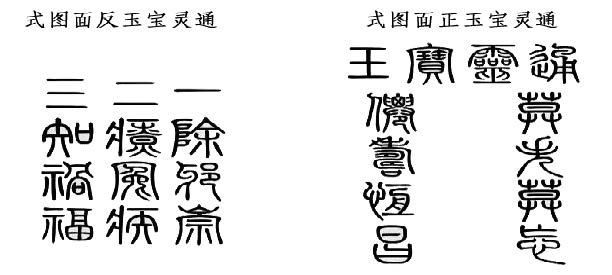
\includegraphics{1-80/8-1}

\begin{qute}

    \begin{parag}\textbf{通靈寶玉反面圖式} \newline
        \indent 三二一\newline
        \indent 知療除\newline
        \indent 禍冤邪\newline
        \indent 福疾崇\newline
    \end{parag}


    \begin{parag}
        \textbf{通靈寶玉正面圖式}\newline
        \indent 仙莫\newline
        \indent 壽失\newline
        \indent 恆莫\newline
        \indent 昌忘\newline
    \end{parag}
\end{qute}


\begin{parag}
    寶釵看畢,\begin{note}甲雙夾:餘亦想見其物矣。前回中總用草蛇灰線寫法,至此方細細寫出,正是大關節處。\end{note}又從新翻過正面來細看,\begin{note}甲側:可謂真奇之至。\end{note}口內念道:“莫失莫忘,仙壽恆昌。”\begin{note}甲側:是心中沉吟,神理。甲眉:《石頭記》立誓一筆不寫一家文字。\end{note}唸了兩遍,乃回頭向鶯兒笑道:“你不去倒茶,也在這裏發呆作什麼?”\begin{note}甲雙夾:請諸公掩卷合目想其神理,想其坐立之勢,想寶釵面上口中。真妙!\end{note}鶯兒嘻嘻笑道:“我聽這兩句話,倒象和姑娘的項圈上的兩句話是一對兒。”\begin{note}甲雙夾:又引出一個金項圈來,鶯兒口中說出方妙。甲眉:恨顰兒不早來聽此數語,若使彼聞之,不知又有何等妙論趣語以悅我等心臆。\end{note}寶玉聽了,忙笑道:“原來姐姐那項圈上也有八個字,\begin{note}甲雙夾:補出素日眼中雖見而實未留心。\end{note}我也鑑賞鑑賞!”寶釵道:“你別聽他的話,沒有什麼字。”寶玉笑央:“好姐姐,你怎麼瞧我的了呢。”寶釵被纏不過,因說道:“也是個人給了兩句吉利話兒,所以鏨上了,叫天天帶著,不然,沉甸甸的有什麼趣兒。”\begin{note}甲雙夾:一句罵死天下濃妝豔飾富貴中之脂妖粉怪。\end{note}一面說,一面解了排扣,\begin{note}甲側:細。\end{note}從裏面大紅襖上將那珠寶晶瑩黃金燦爛的瓔珞掏將出來。\begin{note}甲雙夾:按,瓔珞者,頸飾也!想近俗即呼爲項圈者是矣。\end{note}寶玉忙託了鎖看時,果然一面有四個篆字,兩面八字,共成兩句吉讖。亦曾按式畫下形相:
\end{parag}

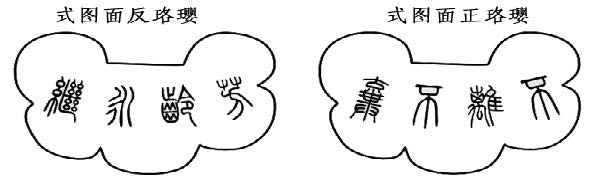
\includegraphics[]{1-80/8-2}

\begin{qute}

    \begin{parag}
        \textbf{瓔珞反面式}
    \end{parag}


    \begin{parag}
        音注云:芳齡永繼。\begin{note}甲側:合前讀之,豈非一對?\end{note}
    \end{parag}


    \begin{parag}
        \textbf{瓔珞正面式}
    \end{parag}


    \begin{parag}
        音注云:不離不棄。
    \end{parag}
\end{qute}


\begin{parag}
    寶玉看了,也念了兩遍,又念自己的兩遍,因笑問:“姐姐這八個字倒真與我的是一對。”\begin{note}甲雙夾:餘亦謂是一對,不知干支中四注八字可與卿亦對否?甲眉:花看半開,酒飲微醉,此文字是也。\end{note}鶯兒笑道:“是個癩頭和尚送的,他說必須鏨在金器上……“\begin{note}和尚在幻境中作如此勾當,亦屬多事。\end{note}寶釵不待說完,便嗔他不去倒茶,\begin{note}甲側:寫寶釵身份。蒙側:雲龍顯影法,好看煞!\end{note}一面又問寶玉從那裏來。\begin{note}甲側:妙神妙理,請觀者自思。\end{note}
\end{parag}


\begin{parag}
    寶玉此時與寶釵就近,只聞一陣陣涼森森甜絲絲的幽香,\begin{note}蒙側:這方是花香襲人正意。\end{note}竟不知系何香氣,遂問:“姐姐燻的是什麼香?我竟從未聞見過這味兒。”\begin{note}甲側:不知比“羣芳髓”又何如?\end{note}寶釵笑道:“我最怕薰香,好好的衣服,燻的煙燎火氣的。”\begin{note}甲側:真真罵死一干濃妝豔飾鬼怪。\end{note}寶玉道:“既如此,這是什麼香?”寶釵想了一想,笑道:“是了,是我早起吃了丸藥的香氣。”\begin{note}甲側:點“冷香丸”。\end{note}寶玉笑道:“什麼丸藥這麼好聞?好姐姐,給我一丸嚐嚐。”\begin{note}甲雙夾:仍是小兒語氣。究竟不知別個小兒,只寶玉如此。\end{note}寶釵笑道:“又混鬧了,一個藥也是混喫的?”
\end{parag}


\begin{parag}
    一語未了,忽聽外面人說:“林姑娘來了。”\begin{note}甲側:緊處愈緊,密不容針之文。\end{note}話猶未了,林黛玉已搖搖\begin{note}甲側:二字畫出身份。\end{note}的走了進來,一見了寶玉,便笑道:“噯喲,我來的不巧了!”\begin{note}甲側:奇文,我實不知顰兒心中是何丘壑。\end{note}寶玉等忙起身笑讓坐,寶釵因笑道:“這話怎麼說?”黛玉笑道:“早知他來,我就不來了。”寶釵道:“我更不解這意。”黛玉笑道:“要來一羣都來,要不來一個也不來,今兒他來了,明兒我再來,如此間錯開了來著,豈不天天有人來了?\begin{note}甲側:強詞奪理。\end{note}也不至於太冷落,也不至於太熱鬧了。\begin{note}甲側:好點綴。\end{note}姐姐如何反不解這意思?”\begin{note}甲雙夾:吾不知顰兒以何物爲心爲齒爲口爲舌,實不知胸中有何丘壑。\end{note}
\end{parag}


\begin{parag}
    寶玉因見他外面罩著大紅羽緞對衿褂子,\begin{note}甲側:岔開文字,避繁章法,妙極妙極!\end{note}\begin{note}蒙側:又一轉換。若無此則必有寶玉之窮究,寶釵之重複,加長無味。此等文章是《西遊記》的請觀世音菩薩,菩薩一到,無不掃地完結者。\end{note}因問:“下雪了麼?”地下婆娘們道:“下了這半日雪珠兒了。”寶玉道:“取了我的斗篷來不曾?”黛玉便道:“是不是,我來了你就該去了。”\begin{note}甲側:實不知有何丘壑。\end{note}寶玉笑道:“我多早晚說要去了?不過拿來預備著。”寶玉的奶母李嬤嬤因說道:“天又下雪,也好早晚的了,就在這裏同姐姐妹妹一處頑頑罷。姨媽那裏擺茶果子呢。我叫丫頭去取了斗篷來,說給小幺兒們散了罷。”寶玉應允。李嬤嬤出去,命小廝們都各散去不提。
\end{parag}


\begin{parag}
    這裏薛姨媽已擺了幾樣細茶果來留他們喫茶。\begin{note}甲側:是溺愛,非勢利。\end{note}寶玉因誇前日在那府裏珍大嫂子的好鵝掌鴨信。\begin{note}甲雙夾:爲前日秦鍾之事恐觀者忘卻,故忙中閒筆,重一渲染。\end{note}薛姨媽聽了,忙也把自己糟的取了些來與他嘗。\begin{note}甲側:是溺愛,非誇富。\end{note}寶玉笑道:“這個須得就酒纔好。”薛姨媽便令人去灌了最上等的酒來。\begin{note}甲側:愈見溺愛。\end{note}李嬤嬤便上來道:“姨太太,酒倒罷了。”\begin{note}甲眉:餘最恨無調教之家,任其子侄肆行哺啜,觀此則知大家風範。\end{note}寶玉央道:“媽媽,我只喝一鍾。”李嬤嬤道:“不中用!當著老太太、太太,那怕你喫一罈呢。想那日我眼錯不見一會,不知是那一個沒調教的,只圖討你的好兒,不管別人死活,給了你一口酒喫,葬送的我捱了兩日罵。姨太太不知道,他性子又可惡,\begin{note}甲側:補出素日。\end{note}吃了酒更弄性。有一日老太太高興了,又盡著他喫,什麼日子又不許他喫,何苦我白賠在裏面。”\begin{note}甲側:浪酒閒茶,原不相宜。\end{note}薛姨媽笑道:“老貨,\begin{note}甲側:二字如聞。\end{note}你只放心喫你的去。我也不許他喫多了。便是老太太問,有我呢。”一面令小丫鬟:“來,讓你奶奶們去,也喫杯搪搪雪氣。”那李嬤嬤聽如此說,只得和衆人去喫些酒水。這裏寶玉又說:“不必溫暖了,我只愛喫冷的。”薛姨媽忙道:“這可使不得,吃了冷酒,寫字手打顫兒。”\begin{note}甲側:酷肖。\end{note}寶釵笑道:“寶兄弟,虧你每日家雜學旁收的,\begin{note}甲側:著眼。若不是寶卿說出,竟不知玉卿日就何業。甲眉:在寶卿口中說出玉兄學業,是作微露卸春掛之萌耳,是書勿看正面爲幸。\end{note}難道就不知道酒性最熱,若熱喫下去,發散的就快,若冷喫下去,便凝結在內,以五臟去暖他,豈不受害?從此還不快不要喫那冷的了。”\begin{note}甲雙夾:知命知身,識理識性,博學不雜,庶可稱爲佳人。可笑別小說中一首歪詩,幾句淫曲,便自佳人相許,豈不醜殺?\end{note}寶玉聽這話有情理,\begin{note}甲雙夾:寶玉亦聽的出有情理的話來,與前回問讀書家務,並皆大奇之事。\end{note}便放下冷酒,命人暖來方飲。
\end{parag}


\begin{parag}
    黛玉磕著瓜子兒,只抿著嘴笑。\begin{note}甲側:實不知其丘壑,自何處設想而來?\end{note}可巧\begin{note}甲側:又用此二字。\end{note}黛玉的小丫鬟雪雁走來與黛玉送小手爐,黛玉因含笑問他:“誰叫你送來的?難爲他費心,那裏就冷死了我!”\begin{note}甲側:吾實不知何爲心,何爲齒、口、舌。\end{note}雪雁道:“紫鵑\begin{note}甲側:鸚哥改名也。\end{note}姐姐\begin{note}甲雙夾:又順筆帶出一個妙名來,洗盡春花臘梅等套。\end{note}怕姑娘冷,使我送來的。”黛玉一面接了,抱在懷中,笑道:“也虧你倒聽他的話。我平日和你說的,全當耳旁風,怎麼他說了你就依,比聖旨還快些!”\begin{note}甲雙夾:要知尤物方如此,莫作世俗中一味酸妒獅吼輩看去。\end{note}寶玉聽這話,知是黛玉藉此奚落他,也無回覆之詞,只嘻嘻的笑兩陣罷了。\begin{note}甲側:這纔好,這纔是寶玉。\end{note}寶釵素知黛玉是如此慣了的,也不去睬他。\begin{note}甲側:渾厚天成,這纔是寶釵。\end{note}薛姨媽因道:“你素日身子弱,禁不得冷的,他們記掛著你倒不好?”黛玉笑道:“姨媽不知道。幸虧是姨媽這裏,倘或在別人家,人家豈不惱?好說就看的人家連個手爐也沒有,巴巴的從家裏送個來。不說丫鬟們太小心過餘,還只當我素日是這等輕狂慣了呢。”\begin{note}甲雙夾:用此一解,真可拍案叫絕,足見其以蘭爲心,以玉爲骨,以蓮爲舌,以冰爲神。真真絕倒天下之裙釵矣。\end{note}\begin{note}甲墨筆眉\begin{subnote}似非脂批,可查看影印本\end{subnote}:強詞奪理,偏他說得如許,真冰雪聰明也\end{note}薛姨媽道:“你這個多心的,有這樣想,我就沒這樣心。”
\end{parag}


\begin{parag}
    說話時,寶玉已是三杯過去。李嬤嬤又上來攔阻。寶玉正在心甜意洽之時,和寶黛姊妹說說笑笑的,\begin{note}甲雙夾:試問石兄:比當日青埂峯猿啼虎嘯之聲何如?\end{note}那肯不喫。寶玉只得屈意央告:“好媽媽,我再喫兩鍾就不吃了。”李嬤嬤道:“你可仔細老爺今兒在家,提防問你的書!”\begin{note}甲側:不入耳之言是也。甲雙夾:不合提此話。這是李嬤嬤激醉了的,無怪乎後文。一笑。\end{note}寶玉聽了這話,便心中大不自在,慢慢的放下酒,垂了頭。\begin{note}甲雙夾:畫出小兒愁蹙之狀,楔緊後文。\end{note}黛玉先忙的說:“別掃大家的興!舅舅\begin{note}甲側:二字指賈政也。\end{note}若叫你,只說姨媽留著呢。這個媽媽,他吃了酒,又拿我們來醒脾了!”\begin{note}甲側:這方是阿顰真意對玉卿之文。\end{note}一面悄推寶玉,使他賭氣,一面悄悄的咕噥說:“別理那老貨,咱們只管樂咱們的。”那李嬤嬤也素知黛玉的意思,因說道:“林姐兒,\begin{note}甲側:如此之稱似不能通,卻是老嫗真心道出。\end{note}你不要助著他了。你倒勸勸他,只怕他還聽些。”林黛玉冷笑道:“我爲什麼助他?我也不犯著勸他。你這媽媽太小心了,往常老太太又給他酒喫,如今在姨媽這裏多喫一口,料也不妨事。必定姨媽這裏是外人,不當在這裏的也未可定。”李嬤嬤聽了,又是急,又是笑,\begin{note}甲側:是認不得真,是不忍認真,是愛極顰兒、疼煞顰兒之意。\end{note}說道:“真真這林姑娘,說出一句話來,比刀子還尖。這算了什麼呢。”寶釵也忍不住笑著,把黛玉腮上一擰,\begin{note}甲側:我也欲擰。\end{note}說道:“真真這個顰丫頭的一張嘴,叫人恨又不是,喜歡又不是。”\begin{note}甲側:可知餘前批不謬。\end{note}薛姨媽一面又說:“別怕,別怕,\begin{note}甲側:是接前老爺問書之語。\end{note}我的兒!來這裏沒好的你喫,別把這點子東西唬的存在心裏,倒叫我不安。只管放心喫,都有我呢。越發吃了晚飯去,便醉了,就跟著我睡罷。”因命:“再燙熱酒來!姨媽陪你喫兩杯,可就喫飯罷。”\begin{note}甲側:二語不失長上之體,且收拾若干文,千斤力量。\end{note}寶玉聽了,方又鼓起興來。
\end{parag}


\begin{parag}
    李嬤嬤因吩咐小丫頭子們:“你們在這裏小心著,我家裏換了衣服就來,悄悄的回姨太太,別由著他,多給他喫。”說著便家去了。這裏雖還有三兩個婆子,都是不關痛癢的,\begin{note}甲側:寫得到。\end{note}見李嬤嬤走了,也都悄悄去尋方便去了。只剩了兩個小丫頭子,樂得討寶玉的歡喜。幸而薛姨媽千哄萬哄的,只容他吃了幾杯,就忙收過了。作酸筍雞皮湯,寶玉痛喝了兩碗,吃了半碗飯碧粳粥。\begin{note}甲側:美粥名。\end{note}一時薛、林二人也喫完了飯,又釅釅的沏上茶來大家吃了。薛姨媽方放了心。雪雁等三四個丫頭已吃了飯,進來伺候。黛玉因問寶玉道:“你走不走?”\begin{note}甲側:妙問。\end{note}寶玉乜斜倦眼\begin{note}甲側:醉意。\end{note}道:“你要走,我和你一同走。”\begin{note}甲側:妙答。此等話,阿顰心中最樂。\end{note}黛玉聽說,遂起身道:“咱們來了這一日,也該回去了。還不知那邊怎麼找咱們呢。”說著,二人便告辭。
\end{parag}


\begin{parag}
    小丫頭忙捧過斗笠來,\begin{note}甲側:不漏。\end{note}寶玉便把頭略低一低,命他戴上。那丫頭便將著大紅氈斗笠一抖,才往寶玉頭上一合,寶玉便說:“罷,罷!好蠢東西,你也輕些兒!難道沒見過別人\begin{note}甲側:“別人”者,襲人、晴雯之輩也。\end{note}戴過的?讓我自己戴罷。”黛玉站在炕沿上道:“羅唆什麼,過來,我瞧瞧罷。”寶玉忙就近前來。黛玉用手整理,輕輕籠住束髮冠,將笠沿掖在抹額之上,將那一顆核桃大的絳絨簪纓扶起,顫巍巍露於笠外。整理已畢,端相了端相,說道:“好了,披上斗篷罷。”\begin{note}甲雙夾:若使寶釵整理,顰卿又不知有多少文章。\end{note}\begin{note}蒙側:知己最難逢,相逢意相同。花新水上香,花下水含紅。\end{note}寶玉聽了,方接了斗篷披上。薛姨媽忙道:“跟你們的媽媽都還沒來呢,且略等等不遲。”寶玉道:“我們倒去等他們,有丫頭們跟著也夠了。”薛姨媽不放心,到底命兩個婦女跟隨他兄妹方罷。他二人道了擾,一徑回至賈母房中。
\end{parag}


\begin{parag}
    賈母尚未用晚飯,知是薛姨媽處來,更加喜歡。\begin{note}甲側:收得好極,正是寫薛家母女。\end{note}因見寶玉吃了酒,遂命他自回房去歇著,不許再出來了。因命人好生看侍著。忽想起跟寶玉的人來,遂問衆人:“李奶子怎麼不見?”\begin{note}甲側:細。\end{note}衆人不敢直說家去了,\begin{note}甲側:有是事,大有是事。\end{note}只說:“才進來的,想有事纔去了。”寶玉踉蹌回頭道:“他比老太太還受用呢,問他作什麼!沒有他只怕我還多活兩日。”一面說,一面來至自己的臥室。只見筆墨在案,\begin{note}甲側:如此找前文最妙,且無逗榫之跡。\end{note}晴雯先接出來,笑說道:“好,好,要我研了那些墨,早起高興,只寫了三個字,丟下筆就走了,哄的我們等了一日。\begin{note}甲側:嬌憨活現,餘雙圈不及。\end{note}快來與我寫完這些墨才罷!”\begin{note}甲側:補前文之未到。\end{note}寶玉忽然想起早起的事來,因笑道:“我寫的那三個字在那裏呢?”晴雯笑道:“這個人可醉了。你頭裏過那府裏去,囑咐貼在這門斗上,這會子又這麼問。我生怕別人貼壞了,\begin{note}甲側:全是體貼一人。\end{note}我親自爬高上梯的貼上,\begin{note}甲側:可見可見。\end{note}這會子還凍的手僵冷的呢。”\begin{note}甲側:可見可見。\end{note}\begin{note}甲雙夾:寫晴雯,是晴雯走下來,斷斷不是襲人、平兒、鶯兒等語氣。\end{note}寶玉聽了,笑\begin{note}甲側:是醉笑。\end{note}道:“我忘了。你的手冷,我替你渥著。”說著便伸手攜了晴雯的手,同仰首看門斗上新書的三個字。\begin{note}甲側:究竟不知是三個什麼字,妙!\end{note}\begin{note}甲眉:誓不作開門見山文字。\end{note}
\end{parag}


\begin{parag}
    一時黛玉來了,寶玉笑道:“好妹妹,你別撒謊,你看這三個字那一個好?”黛玉仰頭看裏間門斗上,新貼了三個字,寫著“絳芸軒”。\begin{note}甲側:出題妙。原來是這三字。\end{note}黛玉笑道:“個個都好。怎麼寫的這們好了?明兒也與我寫一個匾。”\begin{note}甲側:滑賊。\end{note}寶玉嘻嘻的笑道:“又哄我呢。”說著又問:“襲人姐姐呢?”\begin{note}甲側:斷不可少。\end{note}晴雯向裏間炕上努嘴。\begin{note}甲側:畫。\end{note}寶玉一看,只見襲人和衣睡著在那裏。寶玉笑道:“好,太渥早了些。”\begin{note}甲側:絳芸軒中事。\end{note}因又問晴雯道:“今兒我在那府裏喫早飯,有一碟子豆腐皮的包子,我想著你愛喫,和珍大奶奶說了,只說我留著晚上喫,叫人送過來的,你可吃了?”晴雯道:“快別提。一送了來,我知道是我的,偏我才吃了飯,就放在那裏。後來李奶奶來了看見,說:‘寶玉未必吃了,拿了給我孫子喫去罷。’他就叫人拿了家去了。”\begin{note}甲雙夾:奶母之倚勢亦是常情,奶母之昏憒亦是常情。然特於此處細寫一回,與後文襲卿之酥酪遙遙一對,足見晴卿不及襲卿遠矣。餘謂晴有林風,襲乃釵副,真真不假。\end{note}接著茜雪捧上茶來。寶玉因讓:“林妹妹喫茶。”衆人笑說:“林妹妹\begin{note}甲側:三字是接上文口氣而來,非衆人之稱。醉態逼真。\end{note}早走了,還讓呢。”\begin{note}甲眉:寫顰兒去,如此章法從何設想?奇筆奇文。\end{note}
\end{parag}


\begin{parag}
    寶玉吃了半碗茶,忽又想起早起的茶來,\begin{note}甲雙夾:偏是醉人搜尋得出細事,亦是真情。\end{note}因問茜雪道:“早起沏了一碗楓露茶,\begin{note}甲側:與“千紅一窟”遙映。\end{note}我說過,那茶是三四次後纔出色的,這會子怎麼又沏了這個來?”\begin{note}甲側:所謂閒茶是也,與前浪酒一般起落。\end{note}茜雪道:“我原是留著的,那會子李奶奶來了,他要嚐嚐,就給他吃了。”\begin{note}甲側:又是李嬤,事有湊巧,如此類是。\end{note}寶玉聽了,將手中的茶杯只順手\begin{note}甲側:是醉後,故用二字,非有心動氣也。\end{note}往地下一擲,\begin{note}甲眉:按警幻情榜,寶玉系“情不情”。凡世間之無知無識,彼俱有一癡情去體貼。今加“大醉”二字於石兄,是因問包子、問茶、順手擲杯、問茜雪、攆李嬤,乃一部中未有第二次事也。襲人數語,無言而止,石兄真大醉也。甲眉:餘亦云實實大醉也。難辭醉鬧,非薛蟠紈絝輩可比!\end{note}豁啷一聲,打了個粉碎,潑了茜雪一裙子的茶。又跳起來問著茜雪道:“他是你那一門子的奶奶,你們這麼孝敬他?不過是仗著我小時候喫過他幾日奶罷了。\begin{note}甲側:真醉了。\end{note}如今逞的他比祖宗還大了。如今我又喫不著奶了,白白的養著祖宗作什麼!攆了出去,大家乾淨!”\begin{note}甲側:真真大醉了。\end{note}說著便要去立刻回賈母,攆他乳母。
\end{parag}


\begin{parag}
    原來襲人實未睡著,不過故意裝睡,引寶玉來慪他頑耍。先聞得說字問包子等事,也還可不必起來,後來摔了茶鍾,動了氣,遂連忙起來解釋勸阻。早有賈母遣人來問是怎麼了。\begin{note}甲側:斷不可少之文。\end{note}襲人忙道:“我才倒茶來,被雪滑倒了,\begin{note}甲側:現成之至,瞧他寫襲卿爲人。\end{note}失手砸了鍾子。”一面又安慰寶玉道:“你立意要攆他也好,\begin{note}甲側:二字奇,使人一驚。\end{note}我們也都願意出去,不如趁勢連我們一齊攆了,我們也好,你也不愁再有好的來伏侍你。”寶玉聽了這話,方無了言語,被襲人等扶至炕上,脫換了衣服。不知寶玉口內還說些什麼,只覺口齒纏綿,眼眉愈加餳澀,\begin{note}甲側:二字帶出平素形象。\end{note}忙伏侍他睡下。襲人伸手從他項上摘下那通靈玉來,用自己的手帕包好,塞在褥下,次日帶時便冰不著脖子。\begin{note}甲雙夾:試問石兄:此一渥,比青埂峯下松風明月如何?\end{note}那寶玉就枕便睡著了。彼時李嬤嬤等已進來了,聽見醉了,不敢前來再加觸犯,只悄悄的打聽睡了,方放心散去。\begin{note}甲側:交代清楚。“塞玉”一段,又爲“誤竊”一回伏線。晴雯茜雪二婢又爲後文先作一引。甲眉:偷度金針法,最巧。\end{note}
\end{parag}


\begin{parag}
    次日醒來,\begin{note}甲雙夾:以上已完正題,以下是後文引子,前文之餘波。此文收法與前數回不同矣。\end{note}就有人回:“那邊小蓉大爺帶了秦相公來拜。”寶玉忙接了出去,領了拜見賈母。賈母見秦鐘形容標緻,舉止溫柔,堪陪寶玉讀書,\begin{note}甲側:嬌養如此,溺愛如此。\end{note}心中十分歡喜,便留茶留飯,又命人帶去見王夫人等。衆人因素愛秦氏,今見了秦鍾是這般人品,也都歡喜,臨去時都有表禮。賈母又與了一個荷包並一個金魁星,\begin{note}甲眉:作者今尚記金魁星之事乎?撫今思昔,腸斷心摧。\end{note}取“文星和合”之意。又囑咐他道:“你家住的遠,或有一時寒熱飢飽不便,只管住在這裏,不必限定了。只和你寶叔在一處,別跟著那些不長進的東西們學。”\begin{note}甲側:總伏後文。\end{note}秦鍾一一的答應,回去稟知。
\end{parag}


\begin{parag}
    他父親秦業\begin{note}甲雙夾:妙名。業者,孽也,蓋雲情因孽而生也。\end{note}現任營繕郎,\begin{note}甲雙夾:官職更妙,設雲因情孽而繕此一書之意。\end{note}年近七十,夫人早亡。因當年無兒女,便向養生堂抱了一個兒子並一個女兒。誰知兒子又死了,\begin{note}甲側:一頓。\end{note}只剩女兒,小名喚可兒,\begin{note}甲雙夾:出明秦氏究竟不知系出何氏,所謂寓褒貶、別善惡是也。秉刀斧之筆、具菩薩之心亦甚難矣,如此寫出可兒來歷亦甚苦矣。又知作者是欲天下人共來哭此情字。甲眉:寫可兒出身自養生堂,是褒中貶。後死封龍禁尉,是貶中褒。靈巧一至於此。\end{note}長大時,生的形容嫋娜,性格風流。\begin{note}甲側:四字便有隱意。《春秋》字法。\end{note}因素與賈家有些瓜葛,故結了親,許與賈蓉爲妻。那秦業至五旬之上方得了秦鍾。因去歲業師亡故,未暇延請高明之士,只得暫時在家溫習舊課。正思要和親家\begin{note}甲側:指賈珍。\end{note}去商議送往他家塾中,暫且不致荒廢,可巧遇見了寶玉這個機會。又知賈家塾中現今司塾的是賈代儒,\begin{note}甲側:隨筆命名,省事。\end{note}乃當今之老儒,秦鍾此去,學業料必進益,成名可望,因此十分喜悅。只是宦囊羞澀,那賈家上上下下都是一雙富貴眼睛,\begin{note}甲側:爲天下讀書人一哭、寒素人一哭。\end{note}容易拿不出來,又恐誤了兒子的終身大事,\begin{note}甲側:原來讀書是終生大事。\end{note}說不得東拼西湊的恭恭敬敬\begin{note}甲側:四字可思,近之鄙薄師傅者來看。\end{note}封了二十四兩贄見禮,\begin{note}甲雙夾:可知“宦囊羞澀”與“東拼西湊”等樣,是特爲近日守錢虜而不使子弟讀書之輩一大哭。\end{note}親自帶了秦鍾,來代儒家拜見了。然後聽寶玉上學之日,好一同入塾。\begin{note}甲雙夾:不想浪酒閒茶一段金玉旖旎之文後,忽用此等寒瘦古拙之詞收住,亦行文之大變體處。《石頭記》多用此法,歷觀後文便知。\end{note}正是:
\end{parag}


\begin{poem}
    \begin{pl}早知日後閒爭氣,豈肯今朝錯讀書。\end{pl}
    \begin{note}甲側:這是隱語微詞,豈獨此指一事哉?餘則謂讀書正爲爭氣。但此“爭氣”與彼“爭氣”不同。寫來一笑。\end{note}
\end{poem}
\chap{九}{戀風流情友入家塾 起嫌疑頑童鬧學堂}

\begin{parag}
    \begin{note}蒙:君子愛人以道,不能減牽戀之情;小人圖謀以霸,何可逃推頹之辱?幻境幻情,又造出一番小妝新樣。\end{note}
\end{parag}


\begin{parag}
    話說秦業父子專候賈家的人來送上學擇日之信。原來寶玉急於要和秦鐘相遇,\begin{note}蒙雙夾:妙!不知是怎樣相遇。\end{note}卻顧不得別的,遂擇了後日一定上學。“後日一早,請秦相公到我這裏,會齊了,一同前去。”——打發了人送了信。
\end{parag}


\begin{parag}
    至是日一早,寶玉起來時,襲人早已把書筆文物包好,收拾得停停妥妥,坐在牀沿上發悶。\begin{note}蒙側:此等神理,方是此書的正文。蒙雙夾:神理可思,忽又寫小兒學堂中一篇文字,亦別書中未有。\end{note}見寶玉醒來,只得伏待他梳洗。寶玉見他悶悶的,因笑問道:“好姐姐,\begin{note}蒙雙夾:開口斷不可少之三字。\end{note}你怎麼又不自在了?難道怪我上學去丟的你們冷清了不成?”襲人笑道:“這是那裏話。讀書是極好的事,不然就潦倒一輩子,終久怎麼樣呢。但只一件,只是唸書的時節想著書,\begin{note}蒙側:襲人方纔的悶悶,此時的正論,請教諸公,設身處地,亦必是如此方是,真是曲盡情理,一字也不可少者。\end{note}不念的時節想著家些。別和他們一處玩鬧,\begin{note}蒙側:長亭之囑,不過如此。\end{note}碰見老爺不是頑的。雖說是奮志要強,那工課寧可少些,一則貪多嚼不爛,二則身子也要保重。這就是我的意思,你可要體諒。”\begin{note}蒙雙夾:書正語細囑一番。蓋襲卿心中,明知寶玉他並非真心奮志之意,襲人自別有說不出來之語。\end{note}襲人說一句,寶玉答應一句。襲人又道:“大毛衣服我也包好了,交出給小子們去了。學裏冷,好歹想著添換,比不得家裏有人照顧。腳爐手爐的炭也交出去了,你可逼著他們添。那一起懶賊,你不說,他們樂得不動,白凍壞了你。”寶玉道:“你放心,出外頭我自己都會調停的。\begin{note}蒙側:無人體貼,自己扶持。\end{note}你們也別悶死在這屋裏,長和林妹妹一處去頑笑纔好。”說著,俱已穿戴齊備,襲人催他去見賈母、賈政、王夫人等。寶玉且又囑咐了晴雯麝月等幾句,\begin{note}蒙側:這纔是寶玉的本來面目。\end{note}方出來見賈母。賈母也未免有幾句囑咐的話。然後去見王夫人,又出來書房中見賈政。
\end{parag}


\begin{parag}
    偏生這日賈政回家早些,\begin{note}蒙雙夾:若俗筆則又方不在家矣。試想若再不見,則成何文字哉?所謂不敢作安苟且塞責文字。\end{note}正在書房中與相公清客們閒談。忽見寶玉進來請安,回說上學裏去,賈政冷笑道:“你如果再提‘上學’兩個字,連我也羞死了。\begin{note}蒙雙夾:這一句才補出已往許多文字。是嚴父之聲。\end{note}依我的話,你竟頑你的去是正理。仔細站髒了我這地,靠髒了我的門!”\begin{note}蒙雙夾:畫出寶玉的俯首挨壁形象來。\end{note}衆清客相公們都早起身笑道:“老世翁何必又如此。今日世兄一去,三二年就可顯身成名的了,斷不似往年仍作小兒之態了。天也將飯時,世兄竟快請罷。”說著便有兩個年老的攜了寶玉出去。
\end{parag}


\begin{parag}
    賈政因問:“跟寶玉的是誰?”只聽外面答應了兩聲,早進來三四個大漢,打千兒請安。賈政看時,認得是寶玉的奶母之子,名喚李貴。因向他道:“你們成日家跟他上學,他到底唸了些什麼書!倒唸了些流言混話在肚子裏,學了些精緻的淘氣。等我閒一閒,先揭了你的皮,再和那不長進的算賬!”\begin{note}蒙側:此等話似覺無味無理,然而作父母的,到無可如何處,每多用此種法術,所謂百計經營、心力俱瘁者。\end{note}嚇的李貴忙雙膝跪下,摘了帽子,碰頭有聲,連連答應“是”,又回說:“哥兒已經唸到第三本《詩經》,什麼‘呦呦鹿鳴,荷葉浮萍’,小的不敢撒謊。”說的滿座鬨然大笑起來。賈政也掌不住笑了。因說道:“那怕再念三十本《詩經》,也都是掩耳偷鈴,哄人而已。你去請學裏太爺的安,就說我說了:什麼《詩經》古文,一概不用虛應故事,只是先把《四書》一氣講明背熟,是最要緊的。”李貴忙答應“是”,見賈政無話,方退出去。
\end{parag}


\begin{parag}
    此時寶玉獨站在院外屏聲靜候,待他們出來,便忙忙的走了。李貴等一面彈衣服,一面說道:“哥兒可聽見了不曾?可先要揭我們的皮呢!人家的奴才跟主子賺些好體面,我們這等奴才白陪挨打受罵的。從此後也可憐見些纔好。”寶玉笑道:“好哥哥,你別委曲,我明兒請你。”李貴道:“小祖宗,誰敢望你請?只求聽一句半句話就有了。”說著,又至賈母這邊,秦鍾已早來候著了,賈母正和他說話兒呢。\begin{note}蒙雙夾:此處便寫賈母愛秦鍾一如其孫,至後文方不突然。\end{note}於是二人見過,辭了賈母。寶玉忽想起未辭黛玉,\begin{note}蒙雙夾:妙極!何頓挫之至!餘已忘卻,至此心神一暢,一絲不漏。\end{note}因又忙至黛玉房中來作辭。彼時黛玉纔在窗下對鏡理妝,聽寶玉說上學去,因笑道:“好!這一去,可定是要‘蟾宮折桂’去了。\begin{note}蒙側:此寫黛玉,差強人意。《西廂》雙文,能不抱愧!\end{note}我不能送你了。”寶玉道:“好妹妹,等我下學再喫晚飯。和胭脂膏子也等我來再製。”勞叨了半日,方撤身去了。\begin{note}蒙雙夾:如此總一句,更妙!\end{note}黛玉忙又叫住問道:“你怎麼不去辭辭你寶姐姐呢?”寶玉笑而不答。\begin{note}蒙側:黛玉之問,寶玉之笑,兩心一照,何等神工鬼斧之筆。蒙雙夾:必有是語,方是黛玉,此又系黛玉平生之病。\end{note}一徑同秦鐘上學去了。\begin{note}該批:此豈寶玉所樂爲者?然不入家塾則何能有後回“試才”、“結社”文字?作者從不作安逸苟且文字,於此可見。\end{note}\begin{note}該批:此以俗眼讀《石頭記》者,作者之意又豈是俗人所能知。餘謂《石頭記》不得與俗人讀。\end{note}
\end{parag}


\begin{parag}
    原來這賈家義學離此也不甚遠,不過一里之遙,原系始祖所立,恐族中子弟有貧窮不能請師者,即入此中肄業。凡族中有官爵之人,皆供給銀兩,按俸之多寡幫助,爲學中之費。特共舉年高有德之人爲塾掌,專爲訓課子弟。\begin{note}蒙側:創立者之用心,可謂至矣。\end{note}如今寶秦二人來了,一一的都互相拜見過,讀起書來。自此以後,他二人同來同往,同起同坐,愈加親密。又兼賈母愛惜,也時常的留下秦鍾,住上三天五日,與自己的重孫一般疼愛。因見秦鐘不甚寬裕,更又助他些衣履等物。不上一月之工,秦鍾在榮府便熟了。\begin{note}蒙雙夾:交待得清。\end{note}寶玉終是不安分之人,\begin{note}蒙雙夾:寫寶玉總作如此筆。\end{note}\begin{note}靖眉:安分守己,也不是寶玉了。\end{note}竟一味的隨心所欲,因此又發了癖性,又特向秦鍾悄說道:“咱們倆個人一樣的年紀,況又是同窗,以後不必論叔侄,只論弟兄朋友就是了。”\begin{note}蒙側:悄說之時何時?舍尊就卑何心?隨心所欲何癖?相親愛密何情?\end{note}先是秦鐘不肯,當不得寶玉不依,只叫他“兄弟”,或叫他的表字“鯨卿”,秦鍾也只得混著亂叫起來。
\end{parag}


\begin{parag}
    原來這學中雖都是本族人丁與些親戚家的子弟,俗語說的好,“一龍生九種,種種各別。”未免人多了,就有龍蛇混雜,下流人物在內。\begin{note}蒙雙夾:伏一筆。\end{note}自寶、秦二人來了,都生的花朵兒一般的模樣,又見秦鍾靦腆溫柔,未語面先紅,怯怯羞羞,有女兒之風;寶玉又是天生成慣能做小服低,賠身下氣,性情體貼,話語綿纏,\begin{note}蒙雙夾:凡四語十六字,上用“天生成”三字,真正寫盡古今情種人也。\end{note}因此二人更加親厚,也怨不得那起同窗人起了疑,背地裏你言我語,詬誶謠諑,佈滿書房內外。\begin{note}蒙雙夾:伏下文“阿呆爭風”一回。\end{note}
\end{parag}


\begin{parag}
    原來薛蟠自來王夫人處住後,便知有一家學,學中廣有青年子弟,不免偶動了龍陽之興,因此也假來上學讀書,不過是三日打魚,兩日曬網,白送些束脩禮物與賈代儒,卻不曾有一些兒進益,只圖結交些契弟。誰想這學內就有好幾個小學生,圖了薛蟠的銀錢喫穿,被他哄上手的,也不消多記。\begin{note}蒙雙夾:先虛寫幾個淫浪蠢物,以陪下文,方不孤不板。[伏下金榮。]\end{note}更有兩個多情的小學生,\begin{note}蒙雙夾:此處用“多情”二字方妙。\end{note}亦不知是那一房的親眷,亦未考真名姓,\begin{note}蒙雙夾:一併隱其姓名,所謂“具菩提之心,秉刀斧之筆”。\end{note}只因生得嫵媚風流,滿學中都送了他兩個外號,一號“香憐”,一號“玉愛”。誰都有竊慕之意,將不利於孺子之心,\begin{note}蒙雙夾:詼諧得妙,又似李笠翁書中之趣語。\end{note}只是都懼薛蟠的威勢,不敢來沾惹。如今寶、秦二人一來了,見了他兩個,也不免繾綣羨慕,亦因知系薛蟠相知,故未敢輕舉妄動。香、玉二人心中,也一般的留情與寶、秦。因此四人心中雖有情意,只未發跡。每日一入學中,四處各坐,卻八目勾留,或設言托意,或詠桑寓柳,遙以心照,卻外面自爲避人眼目。\begin{note}蒙雙夾:小兒之態活現,掩耳盜鈴者亦然,世人亦復不少。\end{note}不意偏又有幾個滑賊看出形景來,都背後擠眉弄眼,或咳嗽揚聲,\begin{note}蒙側:才子輩偏無不解之事。\end{note}\begin{note}蒙雙夾:又畫出歷來學中一羣頑皮來。\end{note}這也非此一日。
\end{parag}


\begin{parag}
    可巧這日代儒有事,早已回家去了,又留下一句七言對聯,命學生對了,明日再來上書;將學中之事,又命賈瑞\begin{note}蒙雙夾:又出一賈瑞。\end{note}暫且管理。妙在薛蟠如今不大來學中應卯了,因此秦鍾趁此和香憐擠眉弄眼,遞暗號兒,二人假裝出小恭,走至後院說體己話。秦鍾先問他:“家裏的大人可管你交朋友不管?”\begin{note}蒙雙夾:妙問,真真活跳出兩個小兒來。\end{note}一語未了,只聽背後咳嗽了一聲。\begin{note}蒙雙夾:太急了些,該再聽他二人如何結局,正所謂小兒之態也,酷肖之至。\end{note}二人唬的忙回頭看時,原來是窗友名金榮\begin{note}蒙雙夾:妙名,蓋雲有金自榮,廉恥何益哉?\end{note}者。香憐本有些性急,羞怒相激,問他道:“你咳嗽什麼?難道不許我兩個說話不成?”金榮笑道:“許你們說話,難道不許我咳嗽不成?我只問你們:有話不明說,許你們這樣鬼鬼祟祟的幹什麼故事?我可也拿住了,還賴什麼!先得讓我抽個頭兒,咱們一聲兒不言語,不然大家就奮起來。”秦、香二人急得飛紅的臉,便問道:“你拿住什麼了?”金榮笑道:“我現拿住了是真的。”說著,又拍著手笑嚷道:“貼的好燒餅!你們都不買一個喫去?”秦鍾香憐二人又氣又急,忙進來向賈瑞前告金榮,說金榮無故欺負他兩個。
\end{parag}


\begin{parag}
    原來這賈瑞最是個圖便宜沒行止的人,每在學中以公報私,勒索子弟們請他;\begin{note}蒙側:學中亦自有此輩,可爲痛哭。\end{note}後又附助著薛蟠,圖些銀錢酒肉,一任薛蟠橫行霸道,他不但不去管約,反助紂爲虐討好兒。偏那薛蟠本是浮萍心性,今日愛東,明日愛西,近來又有了新朋友,把香、玉二人丟開一邊。就連金榮亦是當日的好朋友,自有了香、玉二人,便棄了金榮。近日連香、玉亦已見棄。故賈瑞也無了提攜幫襯之人,不說薛蟠得新棄舊,只怨香、玉二人不在薛蟠前提攜幫補他,\begin{note}蒙雙夾:無恥小人,真有此心。\end{note}\begin{note}該批:前有幻境遇可卿,今又出學中小兒淫浪之態,後文更放筆寫賈瑞正照。看書人細心體貼,方許你看。\end{note}因此賈瑞金榮等一干人,也正在醋妒他兩個。今兒見秦、香二人來告金榮,賈瑞心中便不自在起來,不好呵叱秦鍾,卻拿著香憐作法,反說他多事,著實搶白了幾句。香憐反討了沒趣,連秦鍾也訕訕的各歸坐位去了。金榮越發得了意,搖頭咂嘴的,口內還說許多閒話,玉愛偏又聽了不忿,兩個人隔座咕咕唧唧的角起口來。金榮只一口咬定說:“方纔明明的撞見他兩個在後院子裏親嘴摸屁股,一對一肏,撅草棍兒抽長短,\begin{note}蒙側:“怎麼長短”四字,何等韻雅,何等渾含!俚語得文人提來,便覺有金玉爲聲之象。\end{note}誰長誰先幹。”金榮只顧得意亂說,卻不防還有別人。誰知早又觸怒了一個。你道這個是誰?
\end{parag}


\begin{parag}
    原來這一個名喚賈薔,\begin{note}蒙雙夾:新而絕,得空便入。\end{note}亦系寧府中之正派玄孫,父母早亡,從小兒跟賈珍過活,如今長了十六歲,比賈蓉生的還風流俊俏。他兄弟二人最相親厚,常相共處。寧府人多口雜,那些不得志的奴僕們,專能造言誹謗主人,因此不知又有了什麼小人詬誶謠諑之辭。賈珍想亦風聞得些口聲不大好,自己也要避些嫌疑,如今竟分與房舍,命賈薔搬出寧府,自去立門戶過活去了。\begin{note}蒙側:此等嫌疑不敢認真搜查,悄爲分計,皆以含而不漏爲文,真實靈活至極之筆。\end{note}這賈薔外相既美,\begin{note}蒙雙夾:亦不免招謗,難怪小人之口。\end{note}內性又聰明,雖然應名來上學,亦不過虛掩眼目而已。仍是鬥雞走狗,賞花玩柳。總恃上有賈珍溺愛,\begin{note}蒙雙夾:貶賈珍最重。\end{note}下有賈蓉匡助,\begin{note}蒙雙夾:貶賈蓉次之。\end{note}因此族中人誰敢來觸逆於他。他既和賈蓉最好,今見有人欺負秦鍾,如何肯依?如今自己要挺身出來報不平,心中卻忖度一番,\begin{note}蒙雙夾:這一忖度,方是聰明人之心機,寫的最好看,最細緻。\end{note}想道:“金榮賈瑞一干人,都是薛大叔的相知,向日我又與薛大叔相好,倘或我一出頭,他們告訴了老薛,\begin{note}蒙雙夾:先曰“薛大叔”,此曰“老薛”,寫盡嬌侈紈絝。\end{note}我們豈不傷和氣?待要不管,如此謠言,說的大家沒趣。如今何不用計制服,又止息了口聲,又不傷了臉面。”想畢,也裝出小恭,走至外面,悄悄的把跟寶玉的書童名喚茗煙\begin{note}蒙雙夾:又出一茗煙。\end{note}者喚到身邊,如此這般調撥他幾句。\begin{note}蒙雙夾:如此便好,不必細述。\end{note}
\end{parag}


\begin{parag}
    這茗煙乃是寶玉第一個得用的,且又年輕不暗世事,如今聽賈薔說金榮如此欺負秦鍾,連他爺寶玉都干連在內,不給他個利害,下次越發狂縱難制了。這茗煙無故就要欺壓人的,如今得了這個信,又有賈薔助著,便一頭進來找金榮,也不叫金相公了,只說:“姓金的,你是什麼東西!”賈薔遂跺一跺靴子,故意整整衣服,看看日影兒說:“是時候了。”遂先向賈瑞說有事要早一步。賈瑞不敢強他,只得隨他去了。這裏茗煙先一把揪住金榮,\begin{note}蒙側:豪奴輩,雖系主人親故亦隨便欺慢,即有一二不服氣者,而豪家多是偏護家人。理之所無,而事之盡有,不知是何心思,是非凡常可能測略。\end{note}問道:“我們肏屁股不肏屁股,管你相干?橫豎沒肏你爹去罷了!你是好小子,出來動一動你茗大爺!”嚇的滿屋中子弟都怔怔的癡望。賈瑞忙吆喝:“茗煙不得撒野!”金榮氣黃了臉,說:“反了!奴才小子都敢如此,我和你主子說。”便奪手要去抓打寶玉秦鍾。\begin{note}蒙雙夾:好看之極!\end{note}尚未去時,從得腦後“颼”的一聲,早見一方硯瓦飛來,\begin{note}蒙雙夾:好看好笑之極!\end{note}並不知系何人打來的,幸未打著,卻又打了旁人的座上,這座上乃是賈藍賈菌。
\end{parag}


\begin{parag}
    賈菌亦系榮府近派的重孫,\begin{note}蒙雙夾:先寫一寧派,又寫一榮派,互相錯綜得妙。\end{note}其母亦少寡,獨守著賈菌,這賈菌與賈藍最好,所以二人同桌而坐。誰知賈菌年紀雖小,志氣最大,極是淘氣不怕人的。\begin{note}蒙雙夾:要知沒志氣小兒,必不會淘氣。\end{note}他在座上冷眼看見金榮的朋友暗助金榮,飛硯來打茗煙,偏沒打著茗煙,便落在他座上,正打在面前,將一個磁硯水壺打了個粉碎,濺了一書黑水。\begin{note}蒙雙夾:這等忙,有此閒處用筆。\end{note}賈菌如何依得,便罵:“好囚攮的們,這不都動了手了麼!”\begin{note}蒙雙夾:好聽煞。靖眉:聲口如聞。\end{note}罵著,也抓起硯磚來要打回去。\begin{note}蒙雙夾:先瓦硯,次磚硯,轉換得妙極。\end{note}賈藍是個省事的,忙按住硯,極口勸道:“好兄弟,不與咱們相干。”\begin{note}蒙雙夾:是賈蘭口氣。\end{note}賈菌如何忍得住,便兩手抱起書匣子來,照那邊掄了去。\begin{note}蒙雙夾:先“飛”後“掄”,用字得神,好看之極!\end{note}終是身小力薄,卻掄不到那裏,剛到寶玉秦鍾桌案上就落了下來,只聽“譁啷啷”一聲,砸在桌上,書本紙片等至於筆硯之物撒了一桌,又把寶玉的一碗茶也砸得碗碎茶流。\begin{note}蒙雙夾:好看之極!不打著別個,偏打著二人,亦想不到文章也。此書此等筆法,與後文踢著襲人、誤打平兒,是一樣章法。\end{note}賈菌便跳出來,要揪打那一個飛硯的。金榮此時隨手抓了一根毛竹大板在手,地狹人多,那裏經得舞動長板。茗煙早吃了一下,亂嚷:“你們還不來動手!”寶玉還有三個小廝:一名鋤藥,一名掃紅,一名墨雨。這三個豈有不淘氣的,一齊亂嚷:“小婦養的!動了兵器了!”\begin{note}蒙雙夾:好聽之極,好看之極!\end{note}墨雨遂掇起一根門閂,掃紅鋤藥手中都是馬鞭子,蜂擁而上。賈瑞急攔一回這個,勸一回那個,誰聽他的話,肆行大鬧。衆頑童也有趁勢幫著打太平拳助樂的,也有膽小藏在一邊的,也有直立在桌上拍著手兒亂笑、喝著聲兒叫打的,登時間鼎沸起來。\begin{note}蒙側:燕青打擂臺,也不過如此。\end{note}
\end{parag}


\begin{parag}
    外邊李貴等幾個大僕人聽見裏邊作反起來,忙都進來一齊喝住。問是何原故。衆聲不一,這一個如此說,那一個又如彼說。\begin{note}蒙雙夾:妙!如聞其聲。\end{note}李貴且喝罵了茗煙四個一頓,攆了出去。\begin{note}蒙雙夾:處治得好。\end{note}秦鐘的頭早撞在金榮的板上,打去一層油皮,寶玉正拿褂襟子替他揉呢,見喝住了衆人,便命:“李貴,收書!拉馬來,我回去回太爺去!我們被人欺負了,不敢說別的,守禮來告訴瑞大爺,瑞大爺反倒派我們不是,聽人家罵我們,還調唆他們打我們茗煙,連秦鐘的頭也打破,這還在這裏念什麼書!茗煙他也是爲有人欺侮我的。不如散了罷。”李貴勸道:“哥兒不要性急。太爺既有事回家去了,這會子爲這點子事去聒噪他老人家,倒顯的咱們沒理。依我的主意,那裏的事那裏了結好,何必去驚動他老人家。這都是瑞大爺的不是,太爺不在這裏,你老人家就是這學裏的頭腦了,衆人看你著行事。\begin{note}蒙側:勸的心思,有個太爺得知,未必然之。故巧爲輾轉以結其局,而不失其體。\end{note}衆人有了不是,該打的打,該罰的罰,如何等鬧到這步田地不管?”賈瑞道:“我吆喝著都不聽。”\begin{note}蒙雙夾:如聞。\end{note}李貴笑道:“不怕你老人家惱我,素日你老人家到底有些不正經,所以這些兄弟纔不聽。就鬧到太爺跟前去,連你老人家也脫不過的。還不快作主意撕羅開了罷。”寶玉道:“撕羅什麼?我必是回去的!”秦鍾哭道:“有金榮,我是不在這裏唸書的。”寶玉道:“這是爲什麼?難道有人家來得的,咱們倒來不得?我必回明白衆人,攆了金榮去。”又問李貴:“金榮是那一房的親戚?”李貴想了一想:“也不用問了。若說起那一房的親戚,更傷了弟兄們的和氣了。”
\end{parag}


\begin{parag}
    茗煙在窗外道:“他是東胡同裏璜大奶奶的侄兒,那是什麼硬正仗腰子的,也來唬我們。璜大奶奶是他姑娘。你那姑媽只會打旋磨子,給我們璉二奶奶跪著借當頭。\begin{note}蒙側:可憐!開口告人,終身是玷。\end{note}我眼裏就看不起他那樣的主子奶奶!”李貴忙斷喝不止,說:“偏你這小狗肏的知道,有這些蛆嚼!”寶玉冷笑道:“我只當是誰的親戚,原來是璜嫂子的侄兒,我就去問問他來!”說著便要走,叫茗煙進來包書。茗煙包著書,又得意道:“爺也不用自己去見,等我去到他家,就說老太太有說的話問他呢,僱上一輛車拉進去,當著老太太問他,豈不省事?”\begin{note}蒙雙夾:又以賈母欺壓,更妙!\end{note}李貴忙喝道:“你要死!仔細回去我好不好先捶了你,然後再回老爺太太,就說寶玉全是你調唆的。我這裏好容易勸哄的好了一半了,你又來生個新法子。你鬧了學堂,不說變法兒壓息了纔是,倒要往大里鬧!”茗煙方不敢作聲兒了。
\end{parag}


\begin{parag}
    此時賈瑞也怕鬧大了,自己也不乾淨,只得委曲著來央告秦鍾,又央告寶玉。先是他二人不肯。後來寶玉說:“不回去也罷了,只叫金榮賠不是便罷。”金榮先是不肯,後來禁不得賈瑞也來逼他去賠不是,李貴等只得好勸金榮說:“原來是你起的端,你不這樣,怎得了局?”金榮強不得,只得與秦鍾作了揖。寶玉還不依,偏定要磕頭。賈瑞只要暫息此事,又悄悄的勸金榮說:“俗語說的好,‘殺人不過頭點地’。你既惹出事來,少不得下點氣兒,磕個頭就完事了。”金榮無奈,只得進前來與秦鍾磕頭。且聽下回分解。
\end{parag}


\begin{parag}
    \begin{note}蒙:此篇寫賈氏學中,非親即族,且學乃大衆之規範,人倫之根本。首先悖亂,以至於此極,其賈家之氣數,即此可知。挾用襲人之風流,羣小之惡逆,一揚一抑,作者自必有所取。\end{note}
\end{parag}


\begin{parag}
    \begin{note}夢:正是:\end{note}
\end{parag}


\begin{parag}
    \begin{note}忍得一時忿,終身無惱悶。\end{note}
\end{parag}


\chap{十}{金寡婦貪利權受辱 張太醫論病細窮源}


\begin{parag}
    \begin{note}蒙:新樣幻情慾收拾,可卿從此世無緣。和肝益氣渾閒事,誰知今日尋病源?\end{note}
\end{parag}


\begin{parag}
    話說金榮因人多勢衆,又兼賈瑞勒令,賠了不是,給秦鍾磕了頭,寶玉方纔不吵鬧了。大家散了學,金榮回到家中,越想越氣,說:“秦鐘不過是賈蓉的小舅子,又不是賈家的子孫,附學讀書,也不過和我一樣。他因仗著寶玉和他好,他就目中無人。他既是這樣,就該行些正經事,人也沒的說。他素日又和寶玉鬼鬼祟祟的,只當我們都是瞎子,看不見。今日他又去勾搭人,偏偏的撞在我眼裏。\begin{note}蒙側:偏是鬼鬼祟祟者,多以爲人不見其行,不知其心。\end{note}就是鬧出事來,我還怕什麼不成?”
\end{parag}


\begin{parag}
    他母親胡氏聽見他咕咕嘟嘟的說,因問道:“你又要爭什麼閒氣?好容易\begin{note}蒙側:“好容易”三字,寫盡天下迎逢要便宜苦惱。\end{note}我望你姑媽說了,你姑媽千方百計的才向他們西府裏的璉二奶奶跟前說了,你才得了這個唸書的地方。若不是仗著人家,咱們家裏還有力量請的起先生?況且人家學裏,茶也是現成的,飯也是現成的。你這二年在那裏唸書,家裏也省好大的嚼用呢。省出來的,你又愛穿件鮮明衣服。再者,不是因你在那裏唸書,你就認得什麼薛大爺了?那薛大爺一年不給不給,這二年也幫了咱們有七八十兩銀子。\begin{note}己側:因何無故給許多銀子?金母亦當細思之。\end{note}\begin{note}蒙側:可憐!婦人愛子,每每如此。自知所得者多,而不知所失者大,可勝嘆者!\end{note}你如今要鬧出了這個學房,再要找這麼個地方,我告訴你說罷,比登天還難呢!\begin{note}己側:如此弄銀,若有金榮在,亦可得。\end{note}你給我老老實實的頑一會子睡你的覺去,好多著呢。”於是金榮忍氣吞聲,不多一時他自去睡了。次日仍舊上學去了。不在話下。
\end{parag}


\begin{parag}
    且說他姑娘,原聘給的是賈家玉字輩的嫡派,名喚賈璜。但其族人那裏皆能象寧榮二府的富勢,原不用細說。這賈璜夫妻守著些小的產業,又時常到寧榮二府裏去請請安,又會奉承鳳姐兒並尤氏,所以鳳姐兒尤氏也時常資助資助他,\begin{note}蒙側:原來根由如此,大與秦鐘不同。\end{note}方能如此度日。今日正遇天氣晴明,又值家中無事,遂帶了一個婆子,坐上車,來家裏走走,瞧瞧寡嫂並侄兒。
\end{parag}


\begin{parag}
    閒話之間,金榮的母親偏提起昨日賈家學房裏的那事,從頭至尾,一五一十都向他小姑子說了。這璜大奶奶不聽則已,聽了,一時怒從心上起,說道:“這秦鍾小崽子是賈門的親戚,難道榮兒不是賈門的親戚?\begin{note}己側:這賈門的親戚比那賈門的親戚。\end{note}人都別忒勢利了,況且都作的是什麼有臉的好事!就是寶玉,也犯不上向著他到這個樣。等我去到東府瞧瞧我們珍大奶奶,再向秦鍾他姐姐說說,叫他評評這個理。\begin{note}己側:未必能如此說。\end{note}\begin{note}蒙側:狗仗人勢者,開口便有多少必勝之談,事要三思,免勞後悔。\end{note}\begin{note}靖側:這個理怕不能評。\end{note}這金榮的母親聽了這話,急的了不得,忙說道:“這都是我的嘴快,告訴了姑奶奶了,求姑奶奶別去,別管他們誰是誰非。\begin{note}己側:不論誰是誰非,有錢就可矣。蒙側:胡氏可謂善哉!\end{note}倘或鬧起來,怎麼在那裏站得住。若是站不住,家裏不但不能請先生,反倒在他身上添出許多嚼用來呢。”璜大奶奶聽了,說道:“那裏管得許多,你等我說了,看是怎麼樣!”也不容他嫂子勸,一面叫老婆子瞧了車,就坐上往寧府裏來。\begin{note}蒙側:何等氣派,何等聲勢,有射石飲羽之力,動天搖地,如項喑吒。\end{note}
\end{parag}


\begin{parag}
    到了寧府,進了車門,到了東邊小角門前下了車,進去見了賈珍之妻尤氏。也未敢氣高,殷殷勤勤敘過寒溫,說了些閒話,方問道:\begin{note}蒙側:何故興致索然?\end{note}“今日怎麼沒見蓉大奶奶?”\begin{note}己側:何不叫秦鐘的姐姐?\end{note}尤氏說道:“他這些日子不知怎麼著,經期有兩個多月沒來。叫大夫瞧了,又說並不是喜。那兩日,到了下半天就懶待動,話也懶待說,眼神也發眩。我說他:‘你且不必拘禮,早晚不必照例上來,你就好生養養罷。就是有親戚一家兒來,有我呢。就有長輩們怪你,等我替你告訴。’連蓉哥我都囑咐了,我說:‘你不許累他,不許招他生氣,叫他靜靜的養養就好了。\begin{note}蒙側:只一絲不露。\end{note}他要想什麼喫,只管到我這裏取來。倘或我這裏沒有,只管望你璉二嬸子那裏要去。倘或他有個好和歹,你再要娶這麼一個媳婦,這麼個模樣兒,這麼個性情的人兒,打著燈籠也沒地方找去。’\begin{note}己側:還有這麼個好小舅子。\end{note}他這爲人行事,那個親戚,那個一家的長輩不喜歡他?所以我這兩日好不煩心,焦的我了不得。偏偏今日早晨他兄弟來瞧他,誰知那小孩子家不知好歹,看見他姐姐身上不大爽快,就有事也不當告訴他,別說是這麼一點子小事,就是你受了一萬分的委曲,也不該向他說纔是。誰知他們昨兒學房裏打架,不知是那裏附學來的一個人欺侮了他了。\begin{note}己側:眼前竟像不知者。蒙側:文筆之妙,妙至於此。本是璜大奶奶不忿來告,又偏從尤氏口中先出,確是秦鍾之語,且是情理必然,形勢逼近。孫悟空七十二變,未有如此靈巧活跳。\end{note}裏頭還有些不乾不淨的話,都告訴了他姐姐。嬸子,你是知道那媳婦的:雖則見了人有說有笑,會行事兒,他可心細,心又重,不拘聽見個什麼話兒,都要度量個三日五夜才罷。這病就是打這個秉性上頭思慮出來的。今兒聽見有人欺負了他兄弟,又是惱,又是氣。惱的是那羣混帳狐朋狗友的扯是搬非、調三惑四那些人;氣的是他兄弟不學好,不上心念書,以致如此學裏吵鬧。他聽了這事,今日索性連早飯也沒喫。我聽見了,我方到他那邊安慰了他一會子,又勸解了他兄弟一會子。我叫他兄弟到那府裏去找寶玉去了,我纔看著他吃了半盞燕窩湯,我纔過來了。嬸子,你說我心焦不心焦?\begin{note}蒙側:這會子金氏聽了這話,心裏當如何料理,實在悔殺從前高興。天下事不得不豫爲三思,先爲防漸。\end{note}況且如今又沒個好大夫,我想到他這病上,我心裏倒象針扎似的。你們知道有什麼好大夫沒有?”\begin{note}蒙側:作無意相問語,是逼近一分,則金氏猶不免當爲分拆。一逼之下,實無可贅之詞。\end{note}
\end{parag}


\begin{parag}
    金氏聽了這半日話,把方纔在他嫂子家的那一團要向秦氏理論的盛氣,早嚇的都丟在爪窪國去了。\begin{note}己側:又何必爲金母著急。\end{note}\begin{note}該批:吾爲趨炎附勢,仰人鼻息者一嘆。\end{note}聽見尤氏問他有知道好大夫的話,連忙答道:“我們這麼聽著,實在也沒見人說有個好大夫。如今聽起大奶奶這個來,定不得還是喜呢。嫂子倒別教人混治。倘或認錯了,這可是了不得的。”尤氏道:“可不是呢。”正是說話間,賈珍從外進來,見了金氏,便向尤氏問道:“這不是璜大奶奶麼?”金氏向前給賈珍請了安。賈珍向尤氏說道:“讓這大妹妹吃了飯去。”賈珍說著話,就過那屋裏去了。\begin{note}靖眉:不知心中作何想。\end{note}金氏此來,原要向秦氏說說秦鍾欺負了他侄兒的事,聽見秦氏有病,不但不能說,亦且不敢提了。況且賈珍尤氏又待的很好,反轉怒爲喜,又說了一會子話兒,方家去了。\begin{note}蒙側:金氏何面目再見江東父老?然而如金氏者,世不乏其人。\end{note}
\end{parag}


\begin{parag}
    金氏去後,賈珍方過來坐下,問尤氏道:“今日他來,有什麼說的事情麼?”尤氏答道:“倒沒說什麼。一進來的時候,臉上倒象有些著了惱的氣色似的,及說了半天話,又提起媳婦這病,他倒漸漸的氣色平定了。你又叫讓他喫飯,他聽見媳婦這麼病,也不好意思只管坐著,又說了幾句閒話兒就去了,倒沒求什麼事。如今且說媳婦這病,你到那裏尋一個好大夫來與他瞧瞧要緊,可別耽誤了。現今咱們家走的這羣大夫,那裏要得?\begin{note}蒙側:醫毒。非止近世,從古有之。\end{note}一個個都是聽著人的口氣兒,人怎麼說,他也添幾句文話兒說一遍。可倒殷勤的很,三四個人一日輪流著倒有四五遍來看脈。他們大家商量著立個方子,吃了也不見效,倒弄得一日換四五遍衣裳,坐起來見大夫,其實於病人無益。”賈珍說道:“可是。這孩子也糊塗,何必脫脫換換的,倘再著了涼,更添一層病,那還了得。衣裳任憑是什麼好的,可又值什麼,孩子的身子要緊,就是一天穿一套新的,也不值什麼。我正進來要告訴你:方纔馮紫英來看我,他見我有些抑鬱之色,問我是怎麼了。我才告訴他說,媳婦忽然身子有好大的不爽快,因爲不得個好太醫,斷不透是喜是病,又不知有妨礙無妨礙,所以我這兩日心裏著實著急。馮紫英因說起他有一個幼時從學的先生,姓張名友士,學問最淵博的,更兼醫理極深,且能斷人的生死。\begin{note}己側:未必能如此。\end{note}\begin{note}蒙側:舉薦人的通套,多是如此說。\end{note}今年是上京給他兒子來捐官,現在他家住著呢。這麼看來,竟是合該媳婦的病在他手裏除災亦未可知。我即刻差人拿我的名帖請去了。\begin{note}蒙側:父母之心,昊天罔極。\end{note}今日倘或天晚了不能來,明日想必一定來。況且馮紫英又即刻回家親自去求他,務必叫他來瞧瞧。等這個張先生來瞧了再說罷。”
\end{parag}


\begin{parag}
    尤氏聽了,心中甚喜,因說道:“後日是太爺的壽日,到底怎麼辦?”賈珍說道:“我方纔到了太爺那裏去請安,兼請太爺來家來受一受一家子的禮。太爺因說道:‘我是清淨慣了的,我不願意往你們那是非場中去鬧去。你們必定說是我的生日,要叫我去受衆人些頭,莫過你把我從前注的《陰騭文》給我令人好好的寫出來刻了,比叫我無故受衆人的頭還強百倍呢。倘或後日這兩日一家子要來,你就在家裏好好的款待他們就是了。也不必給我送什麼東西來,連你後日也不必來,你要心中不安,你今日就給我磕了頭去。\begin{note}蒙側:將寫可卿之好事多慮。至於天生之文中,轉出好清靜之一番議論,清新醒目,立見不凡。\end{note}倘或後日你要來,又跟隨多少人來鬧我,我必和你不依。’如此說了又說,後日我是再不敢去的了。且叫來升來,吩咐他預備兩日的筵席。”尤氏因叫人叫了賈蓉來:“吩咐來升照舊例預備兩日的筵席,要豐豐富富的。你再親自到西府裏去請老太太、大太太、二太太和你璉二嬸子來逛逛。你父親今日又聽見一個好大夫,業已打發人請去了,想必明日必來。你可將他這些日子的病症細細的告訴他。”
\end{parag}


\begin{parag}
    賈蓉一一的答應著出去了。正遇著方纔去馮紫英家請那先生的小子回來了,因回道:“奴才方纔到了馮大爺家,拿了老爺的名帖請那先生去。那先生說道:‘方纔這裏大爺也向我說了。但是今日拜了一天的客,纔回到家,此時精神實在不能支持,就是去到府上也不能看脈。’他說等調息一夜,明日務必到府。\begin{note}蒙側:醫生多是推三阻四,拿腔做調。\end{note}他又說,他‘醫學淺薄,本不敢當此重薦,因我們馮大爺和府上的大人既已如此說了,又不得不去,你先替我回明大人就是了。大人的名帖實不敢當。’仍叫奴才拿回來了。哥兒替奴才回一聲兒罷。”賈蓉轉身復進去,回了賈珍尤氏的話,方出來叫了來升來,吩咐他預備兩日的筵席的話。來升聽畢,自去照例料理。不在話下。
\end{parag}


\begin{parag}
    且說次日午間,人回道:“請的那張先生來了。”賈珍遂延入大廳坐下。茶畢,方開言道:“昨承馮大爺示知老先生人品學問,又兼深通醫學,小弟不勝欽仰之至。”張先生道:“晚生粗鄙下士,本知見淺陋,昨因馮大爺示知,大人家第謙恭下士,又承呼喚,敢不奉命。但毫無實學,倍增顏汗。”賈珍道:“先生何必過謙。就請先生進去看看兒婦,仰仗高明,以釋下懷。”於是,賈蓉同了進去。到了賈蓉居室,見了秦氏,向賈蓉說道:“這就是尊夫人了?”賈蓉道:“正是。請先生坐下,讓我把賤內的病說一說再看脈如何?”那先生道:“依小弟的意思,竟先看過脈再說的爲是。我是初造尊府的,本也不曉得什麼,但是我們馮大爺務必叫小弟過來看看,小弟所以不得不來。如今看了脈息,看小弟說的是不是,再將這些日子的病勢講一講,大家斟酌一個方兒,可用不可用,那時大爺再定奪。”賈蓉道:“先生實在高明,如今恨相見之晚。就請先生看一看脈息,可治不可治,以便使家父母放心。”於是家下媳婦們捧過大迎枕來,一面給秦氏拉著袖口,露出脈來。先生方伸手按在右手脈上,調息了至數,寧神細診了有半刻的工夫,方換過左手,亦復如是。診畢脈息,說道:“我們外邊坐罷。”
\end{parag}


\begin{parag}
    賈蓉於是同先生到外間房裏牀上坐下,一個婆子端了茶來。賈蓉道:“先生請茶。”於是陪先生吃了茶,遂問道:“先生看這脈息,還治得治不得?”先生道:“看得尊夫人這脈息:左寸沉數,左關沉伏,右寸細而無力,右關需而無神。其左寸沉數者,乃心氣虛而生火;左關沉伏者,乃肝家氣滯血虧。右寸細而無力者,乃肺經氣分太虛;右關需而無神者,乃脾土被肝木剋制。心氣虛而生火者,應現經期不調,夜間不寐。肝家血虧氣滯者,必然肋下疼脹,月信過期,心中發熱。肺經氣分太虛者,頭目不時眩暈,寅卯間必然自汗,如坐舟中。脾土被肝木剋制者,必然不思飲食,精神倦怠,四肢痠軟。據我看這脈息,應當有這些症候纔對。或以這個脈爲喜脈,則小弟不敢從其教也。”旁邊一個貼身伏侍的婆子道:“何嘗不是這樣呢。真正先生說的如神,倒不用我們告訴了。如今我們家裏現有好幾位太醫老爺瞧著呢,都不能的當真切的這麼說。有一位說是喜,有一位說是病,這位說不相干,那位說怕冬至,總沒有個準話兒。求老爺明白指示指示。”
\end{parag}


\begin{parag}
    那先生笑\begin{note}蒙側:說是了,不覺笑,描出神情跳躍,如見其人。\end{note}道:“大奶奶這個症候,可是那衆位耽擱了。要在初次行經的日期就用藥治起來,不但斷無今日之患,而且此時已全愈了。如今既是把病耽誤到這個地位,也是應有此災。依我看來,這病尚有三分治得。吃了我的藥看,若是夜裏睡的著覺,那時又添了二分拿手了。據我看這脈息:大奶奶是個心性高強聰明不過的人,聰明忒過,則不如意事常有,不如意事常有,則思慮太過。此病是憂慮傷脾,肝木忒旺,經血所以不能按時而至。大奶奶從前的行經的日子問一問,斷不是常縮,必是常長的。\begin{note}蒙側:恐不合其方,又加一番議論,一方合爲藥,一爲夭亡症,無一字一句不前後照應者。\end{note}是不是?”這婆子答道:“可不是,從沒有縮過,或是長兩日三日,以至十日都長過。”先生聽了道:“妙啊!這就是病源了。從前若能夠以養心調經之藥服之,何至於此。這如今明顯出一個水虧木旺的症候來。待用藥看看。”於是寫了方子,遞與賈蓉,上寫的是:
\end{parag}


\begin{qute2sp}
    益氣養榮補脾和肝湯


    人蔘二錢 白朮二錢土炒 雲苓三錢 熟地四錢


    歸身二錢酒洗 白芍二錢 川芎錢半 黃芪三錢


    香附米二錢制 醋柴胡八分 懷山藥二錢炒 真阿膠二錢蛤粉炒


    延胡索錢半酒炒 炙甘草八分


    引用建蓮子七粒去心 紅棗二枚
\end{qute2sp}


\begin{parag}
    賈蓉看了,說:“高明的很。還要請教先生,這病與性命終久有妨無妨?”先生笑道:“大爺是最高明的人。人病到這個地位,非一朝一夕的症候,吃了這藥也要看醫緣了。依小弟看來,今年一冬是不相干的。總是過了春分,就可望全愈了。”賈蓉也是個聰明人,也不往下細問了。於是賈蓉送了先生去了,方將這藥方子並脈案都給賈珍看了,說的話也都回了賈珍並尤氏了。尤氏向賈珍說道:“從來大夫不象他說的這麼痛快,想必用的藥也不錯。”賈珍道:“人家原不是混飯喫久慣行醫的人。因爲馮紫英我們好,他好容易求了他來了。既有這個人,媳婦的病或者就能好了。他那方子上有人蔘,就用前日買的那一斤好的罷。”賈蓉聽畢話,方出來叫人打藥去煎給秦氏喫。不知秦氏服了此藥病勢如何,下回分解。
\end{parag}


\begin{parag}
    \begin{note}蒙:欲速可卿之死,故先有惡奴之兇頑,而後及以秦鍾來告,層層克入,點露其用心過當,種種文章逼之。雖貧女得居富室,諸凡遂心,終有不能不夭亡之道。我不知作者於著筆時何等妙心繡口,能道此無礙法語,令人不禁眼花撩亂。\end{note}
\end{parag}

\chap{一十一}{慶壽辰寧府排家宴 見熙鳳賈瑞起淫心}

\begin{parag}
    詩曰:
\end{parag}


\begin{poem}
    \begin{pl}一步行來錯,回頭已百年。\end{pl}


    \begin{pl}古今風月鑑,多少泣黃泉!\end{pl}
\end{poem}


\begin{parag}
    \begin{note}蒙:幻境無端換境生,玉樓春暖述乖情。鬧中尋靜渾閒事,運得靈機屬鳳卿。\end{note}
\end{parag}


\begin{parag}
    話說是日賈敬的壽辰,賈珍先將上等可喫的東西,稀奇些的果品,裝了十六大捧盒,著賈蓉帶領家下人等與賈敬送去,向賈蓉說道:“你留神看太爺喜歡不喜歡,你就行了禮來。你說:‘我父親遵太爺的話未敢來,在家裏率領閤家都朝上行了禮了。’”賈蓉聽罷,即率領家人去了。
\end{parag}


\begin{parag}
    這裏漸漸的就有人來了。先是賈璉賈薔到來,先看了各處的座位,並問:“有什麼頑意兒沒有?”家人答道:“我們爺原算計請太爺今日來家來,所以未敢預備頑意兒。前日聽見太爺又不來了,現叫奴才們找了一班小戲兒並一檔子打十番的,都在園子裏戲臺上預備著呢。”
\end{parag}


\begin{parag}
    次後邢夫人、王夫人、鳳姐兒、寶玉都來了,賈珍並尤氏接了進去。尤氏的母親已先在這裏呢。大家見過了,彼此讓了坐。賈珍尤氏二人親自遞了茶,因說道:“老太太原是老祖宗,我父親又是侄兒,這樣日子,原不敢請他老人家,但是這個時候,天氣正涼爽,滿園的菊花又盛開,請老祖宗過來散散悶,看著衆兒孫熱鬧熱鬧,是這個意思。誰知老祖宗又不肯賞臉。”鳳姐兒未等王夫人開口,先說道:“老太太昨日還說要來著呢,因爲晚上看著寶兄弟他們喫桃兒,老人家又嘴饞,吃了有大半個,五更天的時候就一連起來了兩次,\begin{note}蒙側:此一問一答,即景生情,請教是真是假?非身經其事者,想不到,寫不出。\end{note}今日早晨略覺身子倦些。因叫我回大爺,今日斷不能來了,說有好喫的要幾樣,還要很爛的。”\begin{note}蒙側:是。\end{note}賈珍聽了笑道:“我說老祖宗是愛熱鬧的,今日不來,必定有個原故,若是這麼著就是了。”
\end{parag}


\begin{parag}
    王夫人道:“前日聽見你大妹妹說,蓉哥兒媳婦兒身上有些不大好,到底是怎麼樣?”尤氏道:“他這個病得的也奇。上月中秋還跟著老太太,太太們頑了半夜,回家來好好的。到了二十後,一日比一日覺懶,也懶待喫東西,這將近有半個多月了。經期又有兩個月沒來。”邢夫人接著說道:“別是喜罷?”\begin{note}蒙側:此書總是一幅《雲龍圖》。\end{note}
\end{parag}


\begin{parag}
    正說著,外頭人回道:“大老爺,二老爺並一家子的爺們都來了,在廳上呢。”賈珍連忙出去了。這裏尤氏方說道:“從前大夫也有說是喜的。昨日馮紫英薦了他從學過的一個先生,醫道很好,瞧了說不是喜,竟是很大的一個症候。昨日開了方子,吃了一劑藥,今日頭眩的略好些,別的仍不見怎麼樣大見效。”鳳姐兒道:“我說他不是十分支持不住,今日這樣的日子,再也不肯不扎掙著上來。”尤氏道:“你是初三日在這裏見他的,他強扎掙了半天,也是因你們孃兒兩個好的上頭,他才戀戀的捨不得去。”鳳姐兒聽了,眼圈兒紅了半天,半日方說道:“真是‘天有不測風雲,人有旦夕禍福’。\begin{note}蒙側:揣摩的極平常言語來寫無涯之幻景幻情,反作了悟之意,且又轉至別處,真是月下梨花,幾不能辨。\end{note}這個年紀,倘或就因這個病上怎麼樣了,人還活著有甚麼趣兒!”\begin{note}蒙側:大英雄多在此等處悟得,每能超凡入聖。\end{note}正說話間,賈蓉進來,給邢夫人、王夫人、鳳姐兒前都請了安,方回尤氏道:“方纔我去給太爺送喫食去,並回說我父親在家中伺候老爺們,款待一家子的爺們,遵太爺的話未敢來。太爺聽了甚喜歡,說:‘這纔是。’叫告訴父親母親好生伺候太爺太太們,叫我好生伺候叔叔嬸子們並哥哥們。還說那《陰騭文》,叫急急的刻出來,印一萬張散人。我將此話都回了我父親了。我這會子得快出去打發太爺們併合家爺們喫飯。”鳳姐兒說:“蓉哥兒,你且站住。你媳婦今日到底是怎麼著?”賈蓉皺皺眉說道:“不好麼!嬸子回來瞧瞧去就知道了。”\begin{note}蒙側:伏線自然。\end{note}於是賈蓉出去了。
\end{parag}


\begin{parag}
    這裏尤氏向邢夫人,王夫人道:“太太們在這裏喫飯阿,還是在園子裏喫去好?小戲兒現預備在園子裏呢。”王夫人向邢夫人道:“我們索性吃了飯再過去罷,也省好些事。”邢夫人道:“很好。” 於是尤氏就吩咐媳婦婆子們:“快送飯來。”門外一齊答應了一聲,都各人端各人的去了。不多一時,擺上了飯。尤氏讓邢夫人,王夫人並他母親都上了坐,他與鳳姐兒,寶玉側席坐了。邢夫人,王夫人道:“我們來原爲給大老爺拜壽,這不竟是我們來過生日來了麼?”鳳姐兒說道:“大老爺原是好養靜的,已經修煉成了,也算得是神仙了。太太們這麼一說,這就叫作‘心到神知’了。”\begin{note}蒙側:此等趣語,亦不肯無著落。\end{note}一句話說的滿屋裏的人都笑起來了。
\end{parag}


\begin{parag}
    於是,尤氏的母親並邢夫人、王夫人、鳳姐兒都喫畢飯,漱了口,淨了手,才說要往園子裏去,賈蓉進來向尤氏說道:“老爺們並衆位叔叔哥哥兄弟們也都吃了飯了。大老爺說家裏有事,二老爺是不愛聽戲又怕人鬧的慌,都纔去了。別的一家子爺們都被璉二叔並薔兄弟讓過去聽戲去了。方纔南安郡王、東平郡王、西寧郡王、北靜郡王四家王爺,並鎮國公牛府等六家,忠靖侯史府等八家,都差人持了名帖送壽禮來,俱回了我父親,先收在帳房裏了,禮單都上上檔子了。老爺的領謝的名帖都交給各來人了,各來人也都照舊例賞了,衆來人都讓吃了飯纔去了。母親該請二位太太,老孃,嬸子都過園子裏坐著去罷。”\begin{note}蒙側:人送壽禮,是爲園子;回人去的去了在的在,是爲可以過園子裏坐;園子裏坐可以轉入正文中之幻情;幻情裏有乖情,而乖情初寫,偏不乖。真是慧心神手!\end{note}尤氏道:“也是才喫完了飯,就要過去了。”
\end{parag}


\begin{parag}
    鳳姐兒說:“我回太太,我先瞧瞧蓉哥兒媳婦,我再過去。”王夫人道:“很是,我們都要去瞧瞧他,倒怕他嫌鬧的慌,\begin{note}蒙側:爲下文留地步。\end{note}說我們問他好罷。”尤氏道:“好妹妹,媳婦聽你的話,你去開導開導他,我也放心。你就快些過園子裏來。”寶玉也要跟了鳳姐兒去瞧秦氏去,王夫人道:“你看看就過去罷,那是侄兒媳婦。”於是尤氏請了邢夫人,王夫人並他母親都過會芳園去了。
\end{parag}


\begin{parag}
    鳳姐兒、寶玉方和賈蓉到秦氏這邊來。進了房門,悄悄的走到裏間房門口,秦氏見了,就要站起來,鳳姐兒說:“快別起來,看起猛了頭暈。”\begin{note}蒙側:知心每每如此。\end{note}於是鳳姐兒就緊走了兩步,拉住秦氏的手,說道:“我的奶奶!怎麼幾日不見,就瘦的這麼著了!”於是就坐在秦氏坐的褥子上。寶玉也問了好,坐在對面椅子上。賈蓉叫:“快倒茶來,嬸子和二叔在上房還未喝茶呢。”
\end{parag}


\begin{parag}
    秦氏拉著鳳姐兒的手,強笑道:“這都是我沒福。這樣人家,公公婆婆當自己的女孩兒似的待。\begin{note}蒙側:正寫幻情,偏作錐心刺骨語。呼渡河者三,是一意。\end{note}嬸孃的侄兒雖說年輕,卻也是他敬我,我敬他,從來沒有紅過臉兒。就是一家子的長輩同輩之中,除了嬸子倒不用說了,別人也從無不疼我的,也無不和我好的。這如今得了這個病,把我那要強的心一分也沒了。公婆跟前未得孝順一天,就是嬸孃這樣疼我,我就有十分孝順的心,如今也不能夠了。我自想著,未必熬的過年去呢。”
\end{parag}


\begin{parag}
    寶玉正眼瞅著那《海棠春睡圖》並那秦太虛寫的“嫩寒鎖夢因春冷,芳氣籠人是酒香”的對聯,不覺想起在這裏睡晌覺夢到“太虛幻境”的事來。正自出神,聽得秦氏說了這些話,如萬箭攢心,那眼淚不知不覺就流下來了。鳳姐兒心中雖十分難過,但恐怕病人見了衆人這個樣兒反添心酸,倒不是來開導勸解的意思了。見寶玉這個樣子,因說道:“寶兄弟,你忒婆婆媽媽的了。他病人不過是這麼說,那裏就到得這個田地了?況且能多大年紀的人,略病一病兒就這麼想那麼想的,這不是自己倒給自己添病了麼?”賈蓉道:“他這病也不用別的,只是喫得些飲食就不怕了。”\begin{note}蒙側:各人是各人伎倆,一絲不亂,一毫不遺。\end{note}鳳姐兒道:“寶兄弟,太太叫你快過去呢。你別在這裏只管這麼著,倒招的媳婦也心裏不好。太太那裏又惦著你。”因向賈蓉說道:“你先同你寶叔叔過去罷,\begin{note}蒙側:爲本。\end{note}我還略坐一坐兒。”賈蓉聽說,即同寶玉過會芳園來了。
\end{parag}


\begin{parag}
    這裏鳳姐兒又勸解了秦氏一番,又低低的說了許多衷腸話兒,尤氏打發人請了兩三遍,鳳姐兒才向秦氏說道:“你好生養著罷,我再來看你。合該你這病要好,所以前日就有人薦了這個好大夫來,再也是不怕的了。”秦氏笑道:“任憑神仙也罷,治得病治不得命。嬸子,我知道我這病不過是捱日子。”鳳姐兒說道:“你只管這麼想著,病那裏能好呢?總要想開了纔是。況且聽得大夫說,若是不治,怕的是春天不好呢。如今才九月半,還有四五個月的工夫,什麼病治不好呢?咱們若是不能喫人蔘的人家,這也難說了,你公公婆婆聽見治得好你,別說一日二錢人蔘,就是二斤也能夠喫的起。好生養著罷,我過園子裏去了。”秦氏又道:“嬸子,恕我不能跟過去了。閒了時候還求嬸子常過來瞧瞧我,咱們娘兒們坐坐,多說幾遭話兒。”鳳姐兒聽了,不覺得又眼圈兒一紅,遂說道:“我得了閒兒必常來看你。”於是鳳姐兒帶領跟來的婆子丫頭並寧府的媳婦婆子們,從裏頭繞進園子的便門來。\begin{note}蒙側:偏不獨行,用此等反克文字。\end{note}但只見:
\end{parag}


\begin{qute2sp}
    黃花滿地,白柳橫坡。小橋通若耶之溪,曲徑接天台之路。\begin{note}蒙側:點明題目。\end{note}石中清流激湍,籬落飄香,樹頭紅葉翩翻,疏林如畫。西風乍緊,初罷鶯啼,暖日當暄,又添蛩語。遙望東南,建幾處依山之榭,縱觀西北,結三間臨水之軒。笙簧盈耳。別有幽情,羅綺穿林,倍添韻致。
\end{qute2sp}


\begin{parag}
    鳳姐兒正自看園中景緻,一步步行來讚賞。猛然從假山石後走過一個人來,向前對鳳姐兒說道:“請嫂子安。”鳳姐兒猛然見了,將身子望後一退,說道:“這是瑞大爺不是?”賈瑞說道:“嫂子連我也不認得了?不是我是誰!”鳳姐兒道:“不是不認得,猛然一見,不想到是大爺到這裏來。”\begin{note}蒙側:作者何等心思,能在此等事想到如此出言。漸入之妙,無過於此。\end{note}賈瑞道:“也是合該我與嫂子有緣。我方纔偷出了席,在這個清淨地方略散一散,不想就遇見嫂子也從這裏來。這不是有緣麼?”\begin{note}蒙側:重點“有緣”二字,方是筆力。\end{note}一面說著,一面拿眼睛不住的覷著鳳姐兒。
\end{parag}


\begin{parag}
    鳳姐兒是個聰明人,見他這個光景,如何不猜透八九分呢,因向賈瑞假意含笑道:“怨不得你哥哥時常提你,說你很好。今日見了,聽你說這幾句話兒,就知道你是個聰明和氣的人了。這會子我要到太太們那裏去,不得和你說話兒,等閒了咱們再說話兒罷。”賈瑞道:“我要到嫂子家裏去請安,又恐怕嫂子年輕,不肯輕易見人。”鳳姐兒假意笑道:“一家子骨肉,說什麼年輕不年輕的話。”賈瑞聽了這話,再不想到今日得這個奇遇,那神情光景亦發不堪難看了。鳳姐兒說道:“你快入席去罷,仔細他們拿住罰你酒。”賈瑞聽了,身上已木了半邊,慢慢的一面走著,一面回過頭來看。鳳姐兒故意的把腳步放遲了些兒,見他去遠了,心裏暗忖道:“這纔是知人知面不知心呢,那裏有這樣禽獸的人呢!\begin{note}蒙側:大英雄氣概。作者以此命鳳,其有爲耶?\end{note}他如果如此,幾時叫他死在我的手裏,他才知道我的手段!”
\end{parag}


\begin{parag}
    於是鳳姐兒方移步前來。將轉過了一重山坡,見兩三個婆子慌慌張張的走來,見了鳳姐兒,笑說道:“我們奶奶見二奶奶只是不來,急的了不得,叫奴才們又來請奶奶來了。”\begin{note}蒙側:別者必將遇賈瑞的事聲張一番,以表情節。此文偏若無事,一則可以見熙鳳非凡,一則可以見熙鳳包含廣大。\end{note}鳳姐兒說道:“你們奶奶就是這麼急腳鬼似的。”鳳姐兒慢慢的走著,問:“戲唱了幾齣了?”那婆子回道:“有八九出了。”說話之間,已來到了天香樓的後門,見寶玉和一羣丫頭們在那裏玩呢。鳳姐兒說道:“寶兄弟,別忒淘氣了。”\begin{note}蒙側:照應前文。\end{note}有一個丫頭說道:“太太們都在樓上坐著呢,請奶奶就從這邊上去罷。”
\end{parag}


\begin{parag}
    鳳姐兒聽了,款步提衣上了樓,見尤氏已在樓梯口等著呢。尤氏笑說道:“你們孃兒兩個忒好了,見了面總捨不得來了。你明日搬來和他住著罷。你坐下,我先敬你一鍾。”於是鳳姐兒在邢、王二夫人前告了坐,又在尤氏的母親前周旋了一遍,仍同尤氏坐在一桌上喫酒聽戲。尤氏叫拿戲單來,讓鳳姐兒點戲,鳳姐兒說道:“親家太太和太太們在這裏,我如何敢點。”邢夫人王夫人說道:“我們和親家太太都點了好幾出了,你點兩出好的我們聽。”鳳姐兒立起身來答應了一聲,方接過戲單,從頭一看,點了一出《還魂》,一出《彈詞》,遞過戲單去說:“現在唱的這《雙官誥》,\begin{note}蒙側:點下文。\end{note}唱完了,再唱這兩出,也就是時候了。”王夫人道:“可不是呢,也該趁早叫你哥哥嫂子歇歇,他們又心裏不靜。”尤氏說道:“太太們又不常過來,娘兒們多坐一會子去,纔有趣兒,天還早呢。”鳳姐兒立起身來望樓下一看,說:“爺們都往那裏去了?”旁邊一個婆子道:“爺們纔到凝曦軒,帶了打十番的那裏喫酒去了。”鳳姐兒說道:“在這裏不便宜,背地裏又不知幹什麼去了!”\begin{note}蒙側:偏是愛喫酸醋。\end{note}尤氏笑道:“那裏都象你這麼正經人呢。”
\end{parag}


\begin{parag}
    於是說說笑笑,點的戲都唱完了,方纔撤下酒席,擺上飯來。喫畢,大家纔出園子來,到上房坐下,吃了茶,方纔叫預備車,向尤氏的母親告了辭。尤氏率同衆姬妾並家下婆子媳婦們方送出來,賈珍率領衆子侄都在車旁侍立,等候著呢,見了邢夫人王夫人道:“二位嬸子明日還過來逛逛。”王夫人道:“罷了,我們今日整坐了一日,也乏了,明日歇歇罷。”於是都上車去了。賈瑞猶不時拿眼睛覷著鳳姐兒。\begin{note}蒙側:無又不足不盡處。\end{note}賈珍等進去後,李貴才拉過馬來,寶玉騎上,隨了王夫人去了。這裏賈珍同一家子的弟兄子侄喫過了晚飯,方大家散了。
\end{parag}


\begin{parag}
    次日,仍是衆族人等鬧了一日,不必細說。此後鳳姐兒不時親自來看秦氏。秦氏也有幾日好些,也有幾日仍是那樣。賈珍、尤氏、賈蓉好不焦心。\begin{note}蒙側:陪襯補足。\end{note}
\end{parag}


\begin{parag}
    且說賈瑞到榮府來了幾次,偏都遇見鳳姐兒往寧府那邊去了。這年正是十一月三十日冬至。到交節的那幾日,賈母、王夫人、鳳姐兒日日差人去看秦氏,回來的人都說:“這幾日也沒見添病,也不見甚好。”王夫人向賈母說:“這個症候,遇著這樣大節不添病,就有好大的指望了。”賈母說:“可是呢,好個孩子,要是有些原故,可不叫人疼死。”說著,一陣心酸,叫鳳姐兒說道:“你們孃兒兩個也好了一場,明日大初一,過了明日,你後日再去看一看他去。你細細的瞧瞧他那光景,倘或好些兒,你回來告訴我,我也喜歡喜歡。那孩子素日愛喫的,你也常叫人做些給他送過去。”鳳姐兒一一的答應了。
\end{parag}


\begin{parag}
    到了初二日,吃了早飯,來到寧府,看見秦氏的光景,雖未甚添病,但是那臉上身上的肉全瘦幹了。於是和秦氏坐了半日,說了些閒話兒,又將這病無妨的話開導了一遍。秦氏說道:“好不好,春天就知道了。如今現過了冬至,又沒怎麼樣,或者好的了也未可知。嬸子回老太太、太太放心罷。\begin{note}蒙側:文字一變。人於將死時也應有一變。\end{note}昨日老太太賞的那棗泥餡的山藥糕,我倒吃了兩塊,倒象克化的動似的。”鳳姐兒說道:“明日再給你送來。我到你婆婆那裏瞧瞧,就要趕著回去回老太太的話去。”秦氏道:“嬸子替我請老太太、太太安罷。”
\end{parag}


\begin{parag}
    鳳姐兒答應著就出來了,到了尤氏上房坐下。尤氏道:“你冷眼瞧媳婦是怎麼樣?”鳳姐兒低了半日頭,說道:“這實在沒法兒了。你也該將一應的後事用的東西給他料理料理,衝一衝也好。”\begin{note}蒙側:伏下文代辦理喪事。\end{note}尤氏道:“我也叫人暗暗的預備了。就是那件東西不得好木頭,暫且慢慢的辦罷。”於是鳳姐兒吃了茶,說了一會子話兒,說道:“我要快回去回老太太的話去呢。”尤氏道:“你可緩緩的說,別嚇著老太太。”鳳姐兒道:“我知道。”於是鳳姐兒就回來了。到了家中,見了賈母,說:“蓉哥兒媳婦請老太太安,給老太太磕頭,說他好些了,求老祖宗放心罷。他再略好些,還要給老祖宗磕頭請安來呢。”賈母道:“你看他是怎麼樣?”鳳姐兒說:“暫且無妨,精神還好呢。”\begin{note}蒙側:“精神還好呢”五字,寫得出神入化。\end{note}賈母聽了,沉吟了半日,因向鳳姐兒說:“你換換衣服歇歇去罷。”
\end{parag}


\begin{parag}
    鳳姐兒答應著出來,見過了王夫人,到了家中,平兒將烘的家常的衣服給鳳姐兒換了。鳳姐兒方坐下,問道:“家裏沒有什麼事麼?”平兒方端了茶來,遞了過去,說道:“沒有什麼事。就是那三百銀子的利銀,旺兒媳婦送進來,我收了。\begin{note}蒙側:陪。\end{note}再有瑞大爺使人來打聽\begin{note}蒙側:正。\end{note}奶奶在家沒有,\begin{note}蒙側:沒他。\end{note}他要來請安說話。”鳳姐兒聽了,哼了一聲,說道:“這畜生合該作死,看他來了怎麼樣!”平兒因問道:“這瑞大爺是因什麼只管來?”鳳姐兒遂將九月裏寧府園子裏遇見他的光景,他說的話,都告訴了平兒。平兒說道:“癩蛤蟆想天鵝肉喫,沒人倫的混帳東西,起這個念頭,叫他不得好死!”鳳姐兒道:“等他來了,我自有道理。”不知賈瑞來時作何光景,且聽下回分解。
\end{parag}


\begin{parag}
    \begin{note}蒙:將可卿之病將死,作幻情一劫;又將賈瑞之遇唐突,作幻情一變。下回同歸幻境,真風馬牛不相及之談。同範並趨,毫無滯礙,靈活之至,飄飄欲仙。默思作者其人之心,其人之形,其人之神,其人之文,比宋玉、子建一般心性,一流人物。\end{note}
\end{parag}

\chap{一十二}{王熙鳳毒設相思局 賈天祥正照風月鑑}

\begin{parag}
    \begin{note}蒙:反正從來總一心,鏡光至意兩相尋。有朝敲破矇頭甕,綠水青山任好春。\end{note}
\end{parag}


\begin{parag}
    話說鳳姐正與平兒說話,只見有人回說:“瑞大爺來了。”鳳姐急命:\begin{note}庚側:立意追命。\end{note}“快請進來。”賈瑞見往裏讓,心中喜出望外,急忙進來,見了鳳姐,滿面陪笑,\begin{note}庚側:如蛇。\end{note}連連問好。鳳姐兒也假意殷勤,讓坐讓茶。
\end{parag}


\begin{parag}
    賈瑞見鳳姐如此打扮,益發酥倒,因餳了眼問道:“二哥哥怎麼還不回來?”鳳姐道:“不知什麼原故。”賈瑞笑道:“別是路上有人絆住了腳了,\begin{note}蒙側:旁敲遠引。\end{note}捨不得回來也未可知?”鳳姐道:“也未可知。男人家見一個愛一個也是有的。”\begin{note}蒙側:這是鉤。\end{note}賈瑞笑道:\begin{note}庚雙夾:如聞其聲。\end{note}“嫂子這話錯了,我就不這樣。”\begin{note}庚雙夾:漸漸入港。\end{note}鳳姐笑道:“象你這樣的人能有幾個呢,十個裏也挑不出一個來。”\begin{note}庚眉:勿作正面看爲幸。畸笏。蒙側:游魚雖有入甕之志,無鉤不能上岸;一上鉤來,欲去亦不可得。\end{note}賈瑞聽了,喜的抓耳撓腮,又道:“嫂子天天也悶的很?”鳳姐道:“正是呢,只盼個人來說話解解悶兒。”賈瑞笑道:“我倒天天閒著,天天過來替嫂子解解閒悶可好不好?”鳳姐笑道:“你哄我呢,你那裏肯往我這裏來?”賈瑞道:“我嫂子跟前,若有一點謊話,天打雷劈!只因素人聞得人說,嫂子是個利害人,在你跟前一點也錯不得,所以唬住了我。如今見嫂子最是個有說有笑極疼人的,\begin{note}庚雙夾:奇妙!\end{note}我怎麼不來,——死了也願意!”\begin{note}庚側:這倒不假。\end{note}鳳姐笑道:“果然你是個明白人,比賈蓉兩個強遠了。我看他那樣清秀,只當他們心裏明白,誰知竟是兩個糊塗蟲,\begin{note}庚側:反文著眼。\end{note}一點不知人心。”
\end{parag}


\begin{parag}
    賈瑞聽這話,越發撞在心坎兒上,由不得又往前湊了一湊,\begin{note}寫呆人癡性活現。\end{note}覷著眼看鳳姐帶的荷包,然後又問戴著什麼戒指。鳳姐悄悄道 :“放尊重著,別叫丫頭們看了笑話。”賈瑞如聽綸音佛語一般,忙往後退。鳳姐笑道:“你該走了。”\begin{note}庚雙夾:叫去正是叫來也。\end{note}賈瑞道:“我再坐一坐兒。”“好狠心的嫂子!”鳳姐又悄悄的道:“大天白白,人來人往,你就在這裏也不方便。你且去,等著晚上起了更你來,悄悄的在西邊穿堂兒等我。”\begin{note}庚眉:先寫穿堂,只知房舍之大,豈料有許多用處。\end{note}\begin{note}蒙側:凡人在平靜時,物來言至,無不照見。若迷於一事一物,雖風雷交作,有所不聞。即“穿堂爾等”之一語,府第非比凡常,關門戶,必要查看,且更夫僕婦,勢必往來,豈容人藏過於其間?只因色迷,聞聲聯諾,不能有回思之暇,信可悲夫!\end{note}賈瑞聽了,如得珍寶,忙問道:“你別哄我。但只那裏人過的多,怎麼好躲的?”鳳姐道:“你只放心。我把上夜的小廝們都放了假,兩邊門一關,再沒別人了。”賈瑞聽了,喜之不盡,忙忙的告辭而去,心內以爲得手。\begin{note}庚側:未必。\end{note}
\end{parag}


\begin{parag}
    盼到晚上,果然黑地裏摸入榮府,趁掩門時,鑽入穿堂。果見漆黑無人,往賈母那邊去的門戶已鎖倒,只有向東的門未關。賈瑞側耳聽著,半日不見人來,忽聽咯登一聲,東邊的門也倒關了。\begin{note}庚側:平平略施小計。\end{note}賈瑞急的也不敢則聲,只得悄悄的出來,將門撼了撼,關得鐵桶一般。此時要求出去,亦不能夠。\begin{note}蒙側:此大抵是鳳姐調遣。不先爲點明者,可以少許多事故,又可以藏拙。\end{note}南北皆是大房牆,要跳亦無攀援。這屋內又是過門風,空落落;現是臘月天氣,夜又長,朔風凜凜,侵肌裂骨,一夜幾乎不曾凍死。\begin{note}庚眉:可爲偷情一戒。蒙側:教導之法、慈悲之心盡矣,無奈迷徑不悟何!\end{note}好容易盼到早晨,只見一個老婆子先將東門開了,進去叫西門。賈瑞瞅他背著臉,一溜煙抱著肩跑了出來,幸而天氣尚早,人都未起,從後門一徑跑回家去。
\end{parag}


\begin{parag}
    原來賈瑞父母早亡,只有他祖父代儒教養。那代儒素日教訓最嚴,\begin{note}庚眉:教訓最嚴,奈其心何!一嘆。\end{note}不許賈瑞多走一步,生怕他在外喫酒賭錢,有誤學業。今忽見他一夜不歸,只料定他在外非飲即賭,嫖娼宿妓,\begin{note}庚側:輾轉靈活,一人不放,一筆不肖。\end{note}那裏想到這段公案,\begin{note}庚側:世人萬萬想不到,況老學究乎!\end{note}因此氣了一夜。賈瑞也捻著一把汗,少不得回來撒慌,只說:“往舅舅家去了,天黑了,留我住了一夜。”代儒道:“自來出門,非稟我不敢擅出,如何昨日私自去了?據此亦該打,何況是撒謊!”\begin{note}庚眉:處處點父母癡心、子孫不肖。此書系自愧而成。\end{note}因此,發狠到底打了三四十板,不許喫飯,令他跪在院內讀文章,定要補出十天工課來方罷。賈瑞直凍了一夜,今又遭了苦打,且餓著肚子跪在風地裏念文章,\begin{note}教令何嘗不好,孽種故此不同。\end{note}其苦萬狀。\begin{note}庚雙夾:禍福無門,唯人自招。\end{note}
\end{parag}


\begin{parag}
    此時賈瑞前心猶是未改,\begin{note}庚側:四字是尋死之根。庚眉:苦海無邊,回頭是岸。若個能回頭也?嘆嘆!壬午春。畸笏。\end{note}再想不到是鳳姐捉弄他。過後兩日,得了空,便仍來找鳳姐。鳳姐故意抱怨他失信,賈瑞急的賭身發誓。鳳姐因見他自投羅網,\begin{note}庚側:可謂因人而使。\end{note}少不得再尋別計令他知改,\begin{note}庚側:四字是作者明阿鳳身份,勿得輕輕看過。\end{note}故又約他道:“今日晚上,你別在那裏了。你在我這房後小過道子裏那間空屋裏等我,可別冒撞了。”\begin{note}庚雙夾:伏得妙!\end{note}賈瑞道:“果真?”鳳姐道:“誰可哄你,你不信就別來。”\begin{note}庚側:緊一句。\end{note}\begin{note}蒙側:大士心腸。\end{note}賈瑞道:“來,來,來。死也要來!”\begin{note}庚雙夾:不差。\end{note}鳳姐道:“這會子你先去罷。”賈瑞料定晚間必妥,\begin{note}庚側:未必。\end{note}此時先去了。鳳姐在這裏便點兵派將,\begin{note}庚側:四字用得新,必有新文字好看。\end{note}\begin{note}蒙側:新文,最妙!\end{note}設下圈套。
\end{parag}


\begin{parag}
    那賈瑞只盼不到夜上,偏生家裏有親戚又來了,\begin{note}庚雙夾:專能忙中寫閒,狡猾之甚!\end{note}直等吃了晚飯纔去,那天已有掌燈時候。又等他祖父安歇了,方溜進榮府,直往那夾道中屋子裏來等著,熱鍋上的螞蟻一般,\begin{note}蒙側:有心人記著,其實苦惱。\end{note}只是幹轉。左等不見人影,右聽也沒聲音,心下自思:“別是又不來了,又凍我一夜不成?”\begin{note}蒙側:似醒非醒語。\end{note}正自胡猜,只見黑魆魆的來了一個人,\begin{note}庚側:真到了。\end{note}賈瑞便意定是鳳姐,不管皁白,餓虎一般,等那人剛至門前,便如貓兒捕鼠的一般,抱住叫道:“親嫂子,等死我了。”說著,抱到屋裏炕上就親嘴扯褲子,滿口裏“親孃”“親爹”的亂叫起來。\begin{note}蒙側:醜態可笑。\end{note}那人只不做聲,\begin{note}庚側:好極!\end{note}賈瑞拉了自己褲子,硬幫幫的就想頂入。\begin{note}庚側:將到矣。\end{note}忽然燈光一閃,只見賈薔舉著個捻子照道:“誰在屋裏?”只見炕上那人笑道:“瑞大叔要臊我呢。”賈瑞一見,卻是賈蓉,\begin{note}庚雙夾:奇絕!\end{note}真臊的無地可入,\begin{note}庚側:亦未必真。\end{note}不知要怎麼樣纔好,回身就要跑,被賈薔一把揪住道:“別走!如今璉二嬸已經告到太太跟前,\begin{note}庚側:好題目。\end{note}說你無故調戲他。\begin{note}庚眉:調戲還要有故?一笑!\end{note}他暫用了個脫身計,哄你在這邊等著,太太氣死過去,\begin{note}庚側:好大題目。\end{note}因此叫我來拿你。剛纔你又攔住他,沒的說,跟我去見太太!”
\end{parag}


\begin{parag}
    賈瑞聽了,魂不附體,只說:“好侄兒,只說沒有見我,明日我重重的謝你。”賈薔道:“你若謝我,放你不值什麼,只不知你謝我多少?況且口說無憑,寫一文契來。”賈瑞道:“這如何落紙呢?”\begin{note}庚側:也知寫不得。一嘆!\end{note}賈薔道:“這也不妨,寫一個賭錢輸了外人賬目,借頭家銀若干兩便罷。”賈瑞道:“這也容易。只是此時無紙筆。”賈薔道:“這也容易。”說罷,翻身出來,紙筆現成,\begin{note}庚側:二字妙!\end{note}拿來命賈瑞寫。他兩作好作歹,只寫了五十兩銀,然後畫了押,賈薔收起來。然後撕羅賈蓉。\begin{note}蒙側:可憐至此!好事者當自度。\end{note}賈蓉先咬定牙不依,只說:“明日告訴族中的人評評理。”賈瑞急的至於叩頭。賈薔做好做歹的,\begin{note}蒙側:此是加一倍法。\end{note}也寫了一張五十兩欠契才罷。賈薔又道:“如今要放你,我就擔著不是。\begin{note}庚雙夾:又生波瀾。\end{note}老太太那邊的門早已關了,老爺正在廳上看南京的東西,那一條路定難過去,如今只好走後門。若這一走,倘或遇見了人,連我也完了。等我們先去哨探哨探,再來領你。這屋你還藏不得,少時就來堆東西。等我尋個地方。”說畢,拉著賈瑞,仍熄了燈,\begin{note}庚雙夾:細。\end{note}出至院外,摸著大臺磯底下,說道:“這窩兒裏好,你只蹲著,別哼一聲,等我們來再動。”\begin{note}庚側:未必如此收場。\end{note}說畢,二人去了。
\end{parag}


\begin{parag}
    賈瑞此時身不由己,只得蹲在那裏。心下正盤算,只聽頭頂上一聲響,譁拉拉一淨桶尿糞從上面直潑下來,可巧澆了他一頭一身,賈瑞掌不住噯喲了一聲,忙又掩住口,\begin{note}庚雙夾:更奇。\end{note}不敢聲張,滿頭滿臉渾身皆是尿屎,冰冷打戰。\begin{note}庚側:餘料必有新奇解恨文字收場,方是《石頭記》筆力。\end{note}\begin{note}庚眉:瑞奴實當如是報之。此一節可入《西廂記》批評內十大快中。畸笏。\end{note}\begin{note}蒙側:這也未必不是預爲埋伏者。總是慈悲設教,遇難教者,不得不現三頭六臂,並喫人心、喝人血之相,以警戒之耳。\end{note}只見賈薔跑來叫:“快走,快走!”賈瑞如得了命,三步兩步從後門跑到家裏,天已三更,只得叫門。開門人見他這般光景,問是怎的。少不得撒謊說:“黑了,失腳掉在茅廁裏了。”一面到自己房中更衣洗濯,心下方想到是鳳姐頑他,因此發一回恨;再想想鳳姐的模樣兒,\begin{note}庚側:欲根未斷。\end{note}又恨不得一時摟在懷,一夜竟不曾閤眼。
\end{parag}


\begin{parag}
    自此滿心想鳳姐,\begin{note}庚眉:此刻還不回頭,真自尋死路矣。\end{note}\begin{note}蒙側:孫行者非有緊箍兒,雖老君之爐、五行之山,何嘗屈其一二?\end{note}只不敢往榮府去了。賈蓉兩個常常的來索銀子,他又怕祖父知道,正是相思尚且難禁,更又添了債務;日間工課又緊,他二十來歲之人,尚未娶親,邇來想著鳳姐,未免有那指頭告了消乏等事;更兼兩回凍惱奔波,\begin{note}庚雙夾:寫得歷歷病源,如何不死?\end{note}因此三五下里夾攻,\begin{note}庚側:所謂步步緊。\end{note}不覺就得了一病:心內發膨脹,口內無滋味,腳下如綿,眼中似醋,黑夜作燒,白晝常倦,下溺連精,嗽痰帶血。諸如此症,不上一年,都添全了。\begin{note}庚側:簡潔之至!\end{note}於是不能支持,一頭睡倒,合上眼還只夢魂顛倒,滿口亂說胡話,驚怖異常。百般請醫治療,諸如肉桂、附子、鱉甲、麥冬、玉竹等藥,吃了有幾十斤下去,也不見個動靜。\begin{note}庚雙夾:說得有趣。\end{note}
\end{parag}


\begin{parag}
    倏又臘盡春回,這病更又沉重。代儒也著了忙,各處請醫療治,皆不見效。因後來喫“獨蔘湯”,代儒如何有這力量,只得往榮府來尋。王夫人命鳳姐秤二兩給他,\begin{note}庚雙夾:王夫人之慈若是。\end{note}鳳姐回說:“前兒新近都替老太太配了藥,那整的太太又說留著送楊提督的太太配藥,偏生昨兒我已送了去了。”王夫人道:“就是咱們這邊沒了,你打發個人往你婆婆那邊問問,或是你珍大哥哥那府裏再尋些來,湊著給人家。喫好了,救人一命,也是你的好處。”\begin{note}庚雙夾:夾寫王夫人。\end{note}鳳姐聽了,也不遣人去尋,只得將些渣末泡須湊了幾錢,命人送去,只說:\begin{note}蒙側:“只說”。\end{note}“太太送來的,再也沒了。”然後回王夫人說:“都尋了來,共湊了有二兩多送去。”\begin{note}庚雙夾:然便有二兩獨蔘湯,賈瑞固亦不能微好,又豈能望好,但鳳姐之毒何如是?終是瑞之自失也。\end{note}
\end{parag}


\begin{parag}
    那賈瑞此時要命心勝,無藥不喫,只是白花錢,不見效。忽然這日有個跛足道人\begin{note}庚雙夾:自甄士隱隨君一去,別來無恙否?\end{note}來化齋,口稱專治冤業之症。賈瑞偏生在內就聽見了,直著聲叫喊\begin{note}庚雙夾:如聞其聲,吾不忍聽也。\end{note}說:“快請進那位菩薩來救我!”一面叫,一面在枕上叩首。\begin{note}庚雙夾:如見其形,吾不忍看也。\end{note}衆人只得帶了那道士進來。賈瑞一把拉住,連叫:“菩薩救我!”\begin{note}庚雙夾:人之將死,其言也哀,作者如何下筆?\end{note}那道士嘆道:“你這病非藥可醫!我有個寶貝與你,你天天看時,此命可保矣。”說畢,從褡褳中\begin{note}庚雙夾:妙極!此褡褳猶是士隱所搶背者乎?\end{note}取出一面鏡子來\begin{note}庚雙夾:凡看書人從此細心體貼,方許你看,否則此書哭矣。\end{note}——兩面皆可照人,\begin{note}庚雙夾:此書表裏皆有喻也。\end{note}鏡把上面鏨著“風月寶鑑”四字\begin{note}庚雙夾:明點。\end{note}——遞與賈瑞道:“這物出自太虛幻境空靈殿上,警幻仙子所制,\begin{note}庚雙夾:言此書原系空虛幻設。\end{note}\begin{note}庚眉:與“紅樓夢”呼應。\end{note}專治邪思妄動之症,\begin{note}庚雙夾:畢真。\end{note}有濟世保生之功。\begin{note}庚雙夾:畢真。\end{note}所以帶他到世上,單與那些聰明俊傑、風雅王孫等看照。\begin{note}庚雙夾:所謂無能紈絝是也。\end{note}千萬不可照正面,\begin{note}庚側:誰人識得此句!\end{note}\begin{note}庚雙夾:觀者記之,不要看這書正面,方是會看。\end{note}只照他的背面,\begin{note}庚雙夾:記之。\end{note}要緊,要緊!三日後吾來收取,管叫你好了。”說畢,佯常而去,衆人苦留不住。
\end{parag}


\begin{parag}
    賈瑞收了鏡子,想道:“這道士倒有些意思,我何不照一照試試。”想畢,拿起“風月鑑”來,向反面一照,只見一個骷髏立在裏面,\begin{note}庚雙夾:所謂“好知青冢骷髏骨,就是紅樓掩面人”是也。作者好苦心思。\end{note}唬得賈瑞連忙掩了,罵:“道士混賬,如何嚇我!”“我倒再照照正面是什麼。”想著,又將正面一照,只見鳳姐站在裏面招手\begin{note}庚側:可怕是“招手”二字。\end{note}叫他。\begin{note}庚雙夾:奇絕!\end{note}賈瑞心中一喜,盪悠悠的覺得進了鏡子,\begin{note}庚雙夾:寫得奇峭,真好筆墨。\end{note}與鳳姐雲雨一番,鳳姐仍送他出來。到了牀上,“噯喲”了一聲,一睜眼,鏡子從手裏掉過來,仍是反面立著一個骷髏。賈瑞自覺汗津津的,底下已遺了一灘精。\begin{note}蒙側:此一句力如龍象,意謂:正面你方纔已自領略了,你也當思想反面纔是。\end{note}心中到底不足,又翻過正面來,只見鳳姐還招手叫他,他又進去。如此三四次。到了這次,剛要出鏡子來,只見兩個人走來,拿鐵鎖把他套住,拉了就走。\begin{note}庚雙夾:所謂醉生夢死也。\end{note}賈瑞叫道:“讓我拿了鏡子再走!”\begin{note}庚雙夾:可憐!大衆齊來看此。\end{note}\begin{note}蒙側:這是作書者之立意,要寫情種,故於此試一深寫之。在賈瑞則是求仁而得仁,未嘗不含笑九泉,雖死亦不解脫者,悲矣!\end{note}——只說了這句,就再不能說話了。
\end{parag}


\begin{parag}
    旁邊伏侍的賈瑞的衆人,只見他先還拿著鏡子照,落下來,仍睜開眼拾在手內,末後鏡子落下來便不動了。衆人上來看看,已沒了氣,身子底下冰涼漬溼一大灘精,這才忙著穿衣抬牀。代儒夫婦哭的死去活來,大罵道士,“是何妖鏡!\begin{note}庚雙夾:此書不免腐儒一謗。\end{note}若不早毀此物,\begin{note}庚雙夾:凡野史俱可毀,獨此書不可毀。\end{note}遺害於世不小。”\begin{note}庚雙夾:腐儒。\end{note}遂命架火來燒,只聽鏡內哭道:“誰叫你們瞧正面了!你們自己以假爲真,何苦來燒我?”\begin{note}庚雙夾:觀者記之。\end{note}正哭著,只見那跛足道人從外跑來,喊道:“誰毀‘風月鑑’,吾來救也!”說著,直入中堂,搶入手內,飄然去了。
\end{parag}


\begin{parag}
    當下,代儒料理喪事,各處去報喪。三日起經,七日發引,寄靈於鐵檻寺,\begin{note}庚雙夾:所謂“鐵門限”事業。先安一開路道之人,以備秦氏仙柩有方也。\end{note}日後帶回原籍。當下賈家衆人齊來弔問,榮府賈赦贈銀二十兩,賈政亦是二十兩,寧國府賈珍亦有二十兩,別者族中人貧富不等,或三兩五兩,不可勝數。另有各同窗家分資,也湊了二三十兩。代儒家道雖然淡薄,倒也豐豐富富完了此事。
\end{parag}


\begin{parag}
    誰知這年冬底,林如海的書信寄來,卻爲身染重疾,寫書特來接林黛玉回去。\begin{note}蒙側:須要林黛玉長住,偏要暫離。\end{note}賈母聽了,未免又加憂悶,只得忙忙的打點黛玉起身。寶玉大不自在,爭奈父女之情,也不好攔勸。於是賈母定要賈璉送他去,仍叫帶回來。一應土儀盤纏,不消煩說,自然要妥貼。作速擇了日期,賈璉與林黛玉辭別了賈母等,帶領僕從,登舟往揚州去了。要知端的,且聽下回分解。
\end{parag}


\begin{parag}
    \begin{note}庚:此回忽遣黛玉去者,正爲下回可兒之文也。若不遣去,只寫可兒、阿鳳等人,卻置黛玉於榮府,成何文哉?故必遣去,方好放筆寫秦,方不脫髮。況黛玉乃書中正人,秦爲陪客,豈因陪而失正耶?後大觀園方是寶玉、寶釵、黛玉等正經文字,前皆系陪襯之文也。\end{note}
\end{parag}


\begin{parag}
    \begin{note}蒙回末總評:儒家正心,道者煉心,釋輩戒心。可見此心無有不到,無不能入者,獨畏其入於邪而不反,故用正煉戒以縛之。請看賈瑞一起念,及至於死,專誠不二,雖經兩次警教,毫無反悔,可謂癡子,可謂愚情。相乃可思,不能相而獨欲思,豈逃傾頹?作者以此作一新樣情理,以助解者生笑,以爲癡者設以棒喝耳!\end{note}
\end{parag}
\chap{一十三}{秦可卿死封龍禁尉 王熙鳳協理寧國府}

\begin{parag}
    \begin{note}蒙、戚:生死窮通何處真?英明難遏是精神。微密久藏偏自露,幻中夢裏語驚人。\end{note}
\end{parag}


\begin{parag}
    \begin{note}甲:賈珍尚奢,豈有不請父命之理?因敬□□□要緊,不問家事,故得恣意放爲。\end{note}
\end{parag}


\begin{parag}
    \begin{note}
        甲:若明指一州名,似若《西遊》之套,故曰至中之地,不待言可知是光天化日仁風德雨之下矣。不雲國名更妙,可知是堯街舜巷衣冠禮義之鄉矣。直與第一回呼應相接。
    \end{note}
\end{parag}


\begin{parag}
    \begin{note}
        今秦可卿託□□□□□□□□□□□□□理寧府,亦□□□□□□□□□□□□□凡□□□□□□□□□□□□□□□□在封龍禁尉寫乃褒中之貶,隱去天香樓一節,是不忍下筆也。
    \end{note}
    \begin{subnote}按:甲本此頁被對角撕去,故缺字甚多。此頁原有三則評語,第二則與本回庚本眉同。今補。\end{subnote}
\end{parag}


\begin{parag}
    \begin{note}
        庚:此回可卿夢阿鳳,蓋作者大有深意存焉。可惜生不逢時,奈何奈何!然必寫出自可卿之意也,則又有他意寓焉。
    \end{note}
\end{parag}


\begin{parag}
    \begin{note}
        榮、寧世家未有不尊家訓者。雖賈珍尚奢,豈明逆父哉?故寫敬老不管,然後恣意,方見筆筆周到。
    \end{note}
\end{parag}


\begin{parag}
    \begin{note}靖:此回可卿夢阿鳳,作者大有深意,惜已爲末世,奈何奈何!賈珍雖奢淫,豈能逆父哉?特因敬老不管,然後恣意,足爲世家之戒。“秦可卿淫喪天香樓”,作者用史筆也。老朽因有魂託鳳姐賈家後事二件,豈是安富尊榮坐享人能想得到者?其事雖未行,其言其意,令人悲切感服,姑赦之,因命芹溪刪去“遺簪”、“更衣”諸文,是以此回只十頁,刪去天香樓一節,少去四五頁也。\end{note}
\end{parag}


\begin{parag}
    話說鳳姐兒自賈璉送黛玉往揚州去後,心中實在無趣,每到晚間,不過和平兒說笑一回,就胡亂\begin{note}甲側:“胡亂”二字奇。\end{note}睡了。
\end{parag}


\begin{parag}
    這日夜間,正和平兒燈下擁爐倦繡,早命濃薰繡被,二人睡下,屈指算行程該到何處,\begin{note}甲側:所謂“計程今日到梁州”是也。\end{note}不知不覺已交三鼓。平兒已睡熟了。鳳姐方覺星眼微蒙,恍惚只見秦氏從外走來,含笑說道:“嬸嬸好睡!我今日回去,你也不送我一程。因娘兒們素日相好,我捨不得嬸子,故來別你一別。還有一件心願未了,非告訴嬸子,別人未必中用。”\begin{note}甲側:一語貶盡賈家一族空頂冠束帶者。\end{note}
\end{parag}


\begin{parag}
    鳳姐聽了,恍惚問道:“有何心事?你只管託我就是了。”秦氏道:“嬸嬸,你是個脂粉隊裏的英雄,\begin{note}甲側:稱得起。\end{note}連那些束帶頂冠的男子也不能過你,你如何連兩句俗語也不曉得?常言‘月滿則虧,水滿則溢’;又道是‘登高必跌重’。如今我們家赫赫揚揚,已將百載,一日倘或\begin{note}甲側:“倘或”二字酷肖婦女口氣。\end{note}樂極悲生,若應了那句‘樹倒猢猻散’的俗語,\begin{note}甲眉:“樹倒猢猻散”之語,今猶在耳,屈指三十五年矣。哀哉傷哉,寧不痛殺!\end{note}豈不虛稱了一世詩書舊族了!”鳳姐聽了此話,心胸大快,十分敬畏,忙問道:“這話慮的極是,但有何法可以永保無虞?”\begin{note}甲側:非阿鳳不明,該古今名利場中患失之同意也。\end{note}秦氏冷笑道:“嬸子好癡也。否極泰來,榮辱自古週而復始,豈人力能可常保的。但如今能於榮時籌劃下將來衰時的世業,亦可謂常保永全了。即如今日諸事都妥,只有兩件未妥,若把此事如此一行,則後日可保永全了。”
\end{parag}


\begin{parag}
    鳳姐便問何事。秦氏道:“目今祖塋雖四時祭祀,只是無一定的錢糧;第二,家塾雖立,無一定的供給。依我想來,如今盛時固不缺祭祀供給,但將來敗落之時,此二項有何出處?莫若依我定見,趁今日富貴,將祖塋附近多置田莊房舍地畝,以備祭祀供給之費皆出自此處,將家塾亦設於此。合同族中長幼,大家定了則例,日後按房掌管這一年的地畝、錢糧、祭祀、供給之事。如此周流,又無競爭,亦不有典賣諸弊。便是有了罪,凡物可入官,這祭祀產業連官也不入的。便敗落下來,子孫回家讀書務農,也有個退步,\begin{note}蒙雙夾:幻情文字中忽入此等警句,提醒多少熱心人。\end{note}祭祀又可永繼。若目今以爲榮華不絕,不思後日,終非長策。眼見不日又有一件非常喜事,真是烈火烹油、鮮花著錦之盛。要知道,也不過是瞬息的繁華,一時的歡樂,萬不可忘了那‘盛筵必散’的俗語。\begin{note}蒙側:“瞬息繁華,一時歡樂”二語,可共天下有志事業功名者同來一哭。但天生人非無所爲,遇機會,成事業,留名於後世者,辦必有奇傳奇遇,方能成不世之功。此亦皆蒼天暗中扶助,雖有波瀾,而無甚害,反覺其錚錚有聲。其不成也,亦由天命。其好人傾險之計,亦非天命不能行。其繁華歡樂,亦自天命。人於其間,知天命而存好生之心,盡已力以周旋其間,不計其功之成否,所謂心安而理盡,又何患乎?一時瞬息,隨緣遇緣,烏乎不可!\end{note}此時若不早爲後慮,臨期只恐後悔無益了。”\begin{note}甲眉:語語見道,字字傷心,讀此一段,幾不知此身爲何物矣。松齋。\end{note}鳳姐忙問:“有何喜事?”秦氏道:“天機不可泄漏。\begin{note}甲側:伏得妙!\end{note}只是我與嬸子好了一場,臨別贈你兩句話,須要記著。”因念道:
\end{parag}


\begin{poem}
    \begin{pl}三春去後諸芳盡,各自須尋各自門。\end{pl}
    \begin{note}甲側:此句令批書人哭死。甲眉:不必看完,見此二句,即欲墮淚。梅溪。\end{note}
\end{poem}


\begin{parag}
    鳳姐還欲問時,只聽二門上傳事雲牌連叩四下,將鳳姐驚醒。人回:“東府蓉大奶奶沒了。”鳳姐聞聽,嚇了一身冷汗,出了一回神,只得忙忙的穿衣,往王夫人處來。
\end{parag}


\begin{parag}
    彼時閤家皆知,無不納罕,都有些疑心。\begin{note}甲眉:九個字寫盡天香樓事,是不寫之寫。[靖本多署名“棠村”。]庚眉:可從此批。靖眉:可從此批。通回將可卿如何死故隱去,是餘大發慈悲也。嘆嘆!壬午季春。 笏叟。\end{note}那長一輩的想他素日孝順;平一輩的,想他平日和睦親密,\begin{note}庚眉:松齋雲:好筆力。此方是文字佳處。\end{note}下一輩的想他素日慈愛,以及家中僕從老小想他素日憐貧惜賤、慈老愛幼\begin{note}庚側:八字乃爲上人之當銘於五衷。\end{note}之恩,莫不悲嚎痛哭者。\begin{note}庚側:老健。\end{note}
\end{parag}


\begin{parag}
    閒言少敘,卻說寶玉因近日林黛玉回去,剩得自己孤悽,也不和人頑耍,\begin{note}甲側:與鳳姐反對。淡淡寫來,方是二人自幼氣味相投,可知後文皆非突然文字。\end{note}每到晚間便索然睡了。如今從夢中聽見說秦氏死了,連忙翻身爬起來,只覺心中似戮了一刀的不忍,哇的一聲,直奔出一口血來。\begin{note}甲側:寶玉早已看定可繼家務事者可卿也,今聞死了,大失所望。急火攻心,焉得不有此血?爲玉一嘆!\end{note}襲人等慌慌忙忙上來搊(校者注:蒙古王府本此處作“摟”)扶,問是怎麼樣,又要回賈母來請大夫。寶玉笑道:“不用忙,不相干,\begin{note}庚側:又淡淡抹去。\end{note}這是急火攻心,\begin{note}甲側:如何自己說出來了?\end{note}血不歸經。”說著便爬起來,要衣服換了,來見賈母,即時要過去。\begin{note}庚眉:如此總是淡描輕寫,全無痕跡,方見得有生以來,天分中自然所賦之性如此,非因色所感也。\end{note}襲人見他如此,心中雖放不下,又不敢攔,只是由他罷了。賈母見他要去,因說:“才嚥氣的人,那裏不乾淨;二則夜裏風大,明早再去不遲。”寶玉那裏肯依。賈母命人備車,多派跟從人役,擁護前來。
\end{parag}


\begin{parag}
    一直到了寧國府前,只見府門洞開,兩邊燈籠照如白晝,亂烘烘人來人往,裏面哭聲搖山振嶽。\begin{note}甲側:寫大族之喪,如此起緒。\end{note}寶玉下了車,忙忙奔至停靈之室,痛哭一番。然後見過尤氏。誰知尤氏正犯了胃疼舊疾,睡在牀上。\begin{note}甲側:妙!非此何以出阿鳳!\end{note}\begin{note}庚側:緊處愈緊,密處愈密。\end{note}\begin{note}庚眉:所謂層巒疊翠之法也。野史中從無此法。即觀者到此,亦爲寫秦氏未必全到,豈料更又寫一尤氏哉!\end{note}然後又出來見賈珍。彼時賈代儒帶領賈敕、賈效、賈敦、賈赦、賈政、賈琮、賈㻞、賈珩、賈珖、賈琛、賈瓊、賈璘、賈薔、賈菖、賈菱、賈芸、賈芹、賈蓁、賈萍、賈藻、賈蘅、賈芬、賈芳、賈蘭、賈菌、賈芝等\begin{note}庚側:將賈族約略一總,觀者方不惑。\end{note}都來了。賈珍哭的淚人一般,\begin{note}甲側:可笑,如喪考妣,此作者刺心筆也。\end{note}正和賈代儒等說道:“合家大小,遠親近友,誰不知我這媳婦比兒子還強十倍。如今伸腿去了,可見這長房內絕滅無人了。”說著又哭起來。衆人忙勸道:“人已辭世,哭也無益,且商議如何料理要緊。”\begin{note}庚側:淡淡一句,勾出賈珍多少文字來。\end{note}賈珍拍手道:“如何料理,不過盡我所有罷了!”\begin{note}蒙雙夾:“盡我所有”,爲媳婦是非禮之談,父母又將何以待之?故前此有思織酒後狂言,及今復見此語,含而不露,吾不能爲賈珍隱諱。\end{note}
\end{parag}


\begin{parag}
    正說著,只見秦業、秦鍾並尤氏的幾個眷屬\begin{note}甲側:伏後文。\end{note}尤氏姊妹也都來了。賈珍便命賈瓊、賈琛、賈璘、賈薔四個人去陪客,一面吩咐去請欽天監陰陽司來擇日,推準停靈七七四十九日,三日後開喪送訃聞。這四十九日,單請一百單八衆禪僧在大廳上拜大悲懺,超度前亡後化諸魂,以免亡者之罪;另設一罈於天香樓上,\begin{note}甲側:刪卻,是未刪之筆。\end{note}\begin{note}靖眉:何必定用“西”字?讀之令人酸鼻!\end{note}\begin{subnote}按:此條所評正文之「天香樓」,靖藏本作「西帆樓」。\end{subnote}是九十九位全真道士,打四十九日解冤洗業醮。然後停靈於會芳園中,靈前另有五十衆高僧、五十衆高道,對壇按七作好事。那賈敬聞得長孫媳婦死了,因自爲早晚就要飛昇,\begin{note}庚側:可笑可嘆。古今之儒,中途多惑老佛。王梅隱雲:“若能再加東坡十年壽,亦能跳出這圈子來。”斯言信矣。\end{note}\begin{note}蒙側:“就要飛昇”的“要”,用得得當。凡“要”者,則身心急切;急切之者,百事無成。正爲後文作引線。\end{note}如何肯又回家染了紅塵,將前功盡棄呢,因此並不在意,只憑賈珍料理。
\end{parag}


\begin{parag}
    賈珍見父親不管,亦發恣意奢華。看板時,幾副杉木板皆不中用。可巧薛蟠來弔問,因見賈珍尋好板,便說道:“我們木店裏有一副板,叫做什麼檣木,\begin{note}甲眉:檣者,舟具也。所謂“人生若泛舟”而已,寧不可嘆!\end{note}出在潢海鐵網山上,\begin{note}甲側:所謂迷津易墮,塵網難逃也。\end{note}作了棺材,萬年不壞。這還是當年先父帶來,原系義忠親王老千歲要的,因他壞了事,\begin{note}蒙側:“壞了事”等字毒極,寫盡勢利場中故套。\end{note}就不曾拿去。現今還封在店裏,也沒人出價敢買。你若要,就抬來罷了。”賈珍聽了,喜之不盡,即命人抬來。大家看時,只見幫底皆厚八寸,紋若檳榔,味若檀麝,以手扣之,玎璫如金玉。大家都奇異稱賞。賈珍笑問:“價值幾何?”薛蟠笑道:“拿一千兩銀子來,只怕也沒處買去。什麼價不價,賞他們幾兩工錢就是了。”\begin{note}甲側:的是阿呆兄口氣。\end{note}賈珍聽說,忙謝不盡,即命解鋸糊漆。賈政因勸道:“此物恐非常人可享者,\begin{note}甲側:政老有深意存焉。\end{note}殮以上等杉木也就是了。”\begin{note}甲側:夾寫賈政。\end{note}\begin{note}甲眉:寫個個皆到,全無安逸之筆,深得《金瓶》壺奧!\end{note}此時賈珍恨不能代秦氏之死,這話如何肯聽。\begin{note}蒙側:“代秦氏死”等句,總是填實前文。\end{note}
\end{parag}


\begin{parag}
    因忽又聽得秦氏之丫鬟名喚瑞珠者,見秦氏死了,他也觸柱而亡。\begin{note}甲側:補天香樓未刪之文。\end{note}\begin{note}靖側:是亦未刪之筆。\end{note}此事可罕,合族中人也都稱讚。賈珍遂以孫女之禮殮殯,一併停靈於會芳園中之登仙閣。小丫鬟名寶珠者,因見秦氏身無所出,乃甘心願爲義女,誓任摔喪駕靈之任。賈珍喜之不盡,即時傳下,從此皆呼寶珠爲小姐。那寶珠按未嫁女之喪,在靈前哀哀欲絕。\begin{note}甲側:非恩惠愛人,那能如是?惜哉可卿,惜哉可卿!\end{note}於是,合族人丁並家下諸人,都各遵舊制行事,自不敢紊亂。\begin{note}甲側:兩句寫盡大家。\end{note}
\end{parag}


\begin{parag}
    賈珍因想著賈蓉不過是個黌門監,\begin{note}庚側:又起波瀾,卻不突然。\end{note}靈幡經榜上寫時不好看,便是執事也不多,因此心下甚不自在。\begin{note}甲側:善起波瀾。\end{note}可巧這日正是首七第四日,早有大明宮掌宮內相戴權,\begin{note}甲側:妙!大權也。\end{note}先備了祭禮遣人來,次後坐了大轎,打傘嗚鑼,親來上祭。賈珍忙接著,讓至逗蜂軒\begin{note}甲側:軒名可思。\end{note}獻茶。賈珍心中打算定了主意,因而趁便就說要與賈蓉捐個前程的話。戴權會意,因笑道:“想是爲喪禮上風光些?”\begin{note}甲側:難得內相機括之快如此。\end{note}賈珍忙笑道:“老內相所見不差。”戴權道:“事倒湊巧,正有個美缺。如今三百員龍禁尉短了兩員,昨日襄陽侯的兄弟老三來求我,現拿了一千五百兩銀子,送到我家裏。你知道,咱們都是老相與,不拘怎麼樣,看著他爺爺的分上,胡亂應了。\begin{note}甲側:忙中寫閒。\end{note}還剩了一個缺,誰知永興節度使馮胖子來求,要與他孩子捐,我就沒工夫應他。既是咱們的孩子\begin{note}甲側:奇談,畫盡閹官口吻。\end{note}要捐,快寫個履歷來。”賈珍聽說,忙吩咐:“快命書房裏人恭敬寫了大爺的履歷來。”小廝不敢怠慢,去了一刻,便拿了一張紅紙來與賈珍。賈珍看了,忙送與戴權。看時,上面寫道:
\end{parag}


\begin{qute2sp}
    江南江寧府江寧縣監生賈蓉,年二十歲。曾祖,原任京營節度使世襲一等神威將軍賈代化;祖,乙卯科進士賈敬;父,世襲三品爵威烈將軍賈珍。
\end{qute2sp}


\begin{parag}
    戴權看了,回手便遞與一個貼身的小廝收了,說道:“回來送與戶部堂官老趙,說我拜上他,起一張五品龍禁尉的票,再給個執照,就把那履歷填上,明兒我來兌銀子送去。”小廝答應了,戴權也就告辭了。賈珍十分款留不住,只得送出府門。臨上轎,賈珍因問:“銀子還是我到部兌,還是一併送入老內相府中?”戴權道:“若到部裏,你又喫虧了。不如平準一千二百銀子送到我家裏就完了。”賈珍感謝不盡,只說:“待服滿後,親帶小犬到府叩謝。”於是作別。
\end{parag}


\begin{parag}
    接著,便又聽喝道之聲,原來是忠靖侯史鼎的夫人來了。\begin{note}甲側:史小姐湘雲消息也。\end{note}王夫人、邢夫人、鳳姐等剛迎入上房,又見錦鄉侯、川寧侯、壽山伯三家祭禮擺在靈前。少時,三人下轎,賈政等忙接上大廳。如此親朋你來我去,也不能勝數。只這四十九日,\begin{note}庚側:就簡去繁。\end{note}寧國府街上一條白漫漫人來人往,\begin{note}甲側:是有服親朋並家下人丁之盛。\end{note}花簇簇官去官來。\begin{note}甲側:是來往祭弔之盛。\end{note}
\end{parag}


\begin{parag}
    賈珍命賈蓉次日換了吉服,領憑回來。靈前供用執事等物,俱按五品職例。靈牌疏上皆寫“天朝誥授賈門秦氏恭人之靈位”。會芳園臨街大門洞開,旋在兩邊起了鼓樂廳,兩班青衣按時奏樂,一對對執事擺的刀斬斧齊。更有兩面硃紅銷金大字牌對豎在門外,上面大書:“防護內廷紫禁道御前侍衛龍禁尉”。對面高起著宣壇,僧道對壇榜文,榜上大書:“世襲寧國公冢孫婦、防護內廷御前侍衛龍禁尉賈門秦氏恭人之喪。\begin{note}庚眉:賈珍是亂費,可卿卻實如此。\end{note}四大部州至中之地,奉天承運太平之國,\begin{note}庚眉:奇文。若明指一州名,似若《西遊》之套,故曰至中之地,不待言可知是光天化日仁風德雨之下矣。不雲國名更妙,可知是堯街舜巷衣冠禮義之鄉矣。直與第一回呼應相接。\end{note}總理虛無寂靜教門僧錄司正堂萬虛、總理元始三一教門道錄司正堂葉生等,敬謹修齋,朝天叩佛”,以及“恭請諸伽藍、揭諦、功曹等神,聖恩普錫,神威遠鎮,四十九日消災洗業平安水陸道場”等語,亦不消繁記。
\end{parag}


\begin{parag}
    只是賈珍雖然此時心意滿足,\begin{note}蒙側:可笑。\end{note}但裏面尤氏又犯了舊疾,不能料理事務,惟恐各誥命來往,虧了禮數,怕人笑話,因此心中不自在。當下正憂慮時,因寶玉\begin{note}甲側:餘正思如何高擱起玉兄了。\end{note}在側問道:“事事都算安貼了,大哥哥還愁什麼?”賈珍見問,便將裏面無人的話說了出來。寶玉聽說笑道:“這有何難,我薦一個人\begin{note}甲側:薦鳳姐須得寶玉,俱龍華會上人也。\end{note}與你權理這一個月的事,管必妥當。”賈珍忙問:“是誰?”寶玉見座間還有許多親友,不便明言,走至賈珍耳邊說了兩句。賈珍聽了喜不自禁,連忙起身道:“果然安貼,如今就去。”說著拉了寶玉,辭了衆人,便往上房裏來。
\end{parag}


\begin{parag}
    可巧這日非正經日期,親友來的少,裏面不過幾位近親堂客,邢夫人、王夫人、鳳姐併合族中的內眷陪坐。聞人報:“大爺進來了。”唬的衆婆娘唿的一聲,往後藏之不迭,\begin{note}甲側:數日行止可知。作者自是筆筆不空,批者亦字字留神之至矣。\end{note}獨鳳姐款款站了起來。\begin{note}庚側:又寫鳳姐。\end{note}賈珍此時也有些病症在身,二則過於悲痛了,因拄拐踱了進來。邢夫人等因說道:“你身上不好,又連日事多,該歇歇纔是,又進來做什麼?”賈珍一面扶拐,\begin{note}庚側:一絲不亂。\end{note}\begin{note}靖眉:刺心之筆。\end{note}扎掙著要蹲身跪下請安道乏。邢夫人等忙叫寶玉攙住,命人挪椅子來與他坐。賈珍斷不肯坐,因勉強陪笑道:“侄兒進來有一件事要求二位嬸子並大妹。”邢夫人等忙問:“什麼事?”賈珍忙道:“嬸子自然知道,如今孫子媳婦沒了,侄兒媳婦偏又病倒,我看裏頭著實不成個體統。怎麼屈尊大妹妹一個月,\begin{note}庚側:不見突然。\end{note}在這裏料理料理,我就放心了。”\begin{note}庚側:阿鳳此刻心癢矣。\end{note}邢夫人笑道:“原來爲這個。你大妹妹現在你二嬸子家,只和你二嬸子說就是了。”王夫人忙道:“他一個小孩子\begin{note}庚側:三字愈令人可愛可憐。\end{note}家何曾經過這樣事,倘或料理不清,反叫人笑話,倒是再煩別人好。”賈珍笑道:“嬸子的意思侄兒猜著了,是怕大妹妹勞苦了。若說料理不開,我包管必料理的開,便是錯一點兒,別人看著還是不錯的。從小兒大妹妹頑笑著就有殺伐決斷,\begin{note}庚側:阿鳳身份。\end{note}如今出了閣,又在那府裏辦事,越發歷練老成了。我想了這幾日,除了大妹妹再無人了。嬸子不看侄兒、侄兒媳婦的分上,只看死了的分上罷!”說著滾下淚來。\begin{note}庚側:有筆力。\end{note}
\end{parag}


\begin{parag}
    王夫人心中怕的是鳳姐未經過喪事,怕他料理不清,惹人恥笑。今見賈珍苦苦的說到這步田地,心中已活了幾分,卻又眼看著鳳姐出神。那鳳姐素日最喜攬事辦,好賣弄才幹,雖然當家妥當,也因未辦過婚喪大事,恐人還不伏,巴不得遇見這事。今見賈珍如此一來,他心中早已歡喜。先見王夫人不允,後見賈珍說的情真,王夫人有活動之意,便向王夫人道:“大哥哥說的這麼懇切,太太就依了罷。”王夫人悄悄的道:“你可能麼?”鳳姐道:“有什麼不能的。外面的大事已經大哥哥\begin{note}庚旁批:王夫人是悄言,鳳姐是響應,故稱“大哥哥”。\end{note}料理清了,\begin{note}庚側:已得三昧矣。\end{note}不過是裏頭照管照管,便是我有不知道的,問問太太就是了。”\begin{note}甲側:胸中成見已有之語。\end{note}王夫人見說的有理,便不作聲。賈珍見鳳姐允了,又陪笑道:“也管不得許多了,橫豎要求大妹妹辛苦辛苦。我這裏先與妹妹行禮,等事完了,我再到那府裏去謝。”說著,就作揖下去,鳳姐兒還禮不迭。
\end{parag}


\begin{parag}
    賈珍便忙向袖中取了寧國府對牌出來,命寶玉送與鳳姐,又說:“妹妹愛怎樣就怎樣,要什麼只管拿這個取去,也不必問我。只求別存心替我省錢,只要好看爲上;二則也要同那府裏一樣待人才好,不要存心怕人抱怨。只這兩件外,我再沒不放心的了。”鳳姐不敢就接牌,\begin{note}蒙雙夾:凡有本領者斷不越禮。接牌小事而必待命於王夫人也,誠家道之規範,亦天下之規範也。看是書者不可草草從事。\end{note}只看著王夫人。王夫人道:“你哥哥既這麼說,你就照看照看罷了。只是別自作主意,有了事,打發人問你哥哥、嫂子要緊。”寶玉早向賈珍手裏接過對牌來,強遞與鳳姐了。又問:“妹妹住在這裏,還是天天來呢?若是天天來,越發辛苦了。不如我這裏趕著收拾出一個院落來,妹妹住過這幾日倒安穩。”鳳姐笑道:“不用。\begin{note}甲側:二字句,有神。\end{note}那邊也離不得我,倒是天天來的好。”賈珍聽說,只得罷了。然後又說了一回閒話,方纔出去。
\end{parag}


\begin{parag}
    一時女眷散後,王夫人因問鳳姐:“你今兒怎麼樣?”鳳姐兒道:“太太只管請回去,我須得先理出一個頭緒來,纔回去得呢。”王夫人聽說,便先同邢夫人等回去,不在話下。
\end{parag}


\begin{parag}
    這裏鳳姐兒來至三間一所抱廈內坐了,因想:頭一件是人口混雜,遺失東西;第二件,事無專責,臨期推委;第三件,需用過費,濫支冒領;第四件,任無大小,苦樂不均;第五件,家人豪縱,有臉者不服鈐束,無臉者不能上進。\begin{note}甲眉:舊族後輩受此五病者頗多,餘家更甚。三十年前事見書於三十年後,令餘悲痛血淚盈面。\end{note}\begin{note}庚眉:讀五件事未完,餘不禁失聲大哭,三十年前作書人在何處耶?\end{note}此五件實是寧國府中風俗。不知鳳姐如何處治,且聽下回分解。\begin{note}甲眉:此回只十頁,因刪去天香樓一節,少去四五頁也。\end{note}
\end{parag}


\begin{parag}
    正是:
\end{parag}


\begin{poem}
    \begin{pl} 金紫萬千誰治國,裙釵一二可齊家。\end{pl}
    \begin{note}蒙:五件事若能如法整理得當,豈獨家庭,國家天下治之不難。\end{note}
\end{poem}


\begin{parag}
    \begin{note}甲:“秦可卿淫喪天香樓”,作者用史筆也。老朽因有魂託鳳姐賈家後事二件,的是安富尊榮坐享人不能想得到處。其事雖未行,其言其意則令人悲切感服,姑赦之,因命芹溪刪去。\end{note}
\end{parag}


\begin{parag}
    \begin{note}庚:通回將可卿如何死故隱去,是大發慈悲心也,嘆嘆!壬午春。\end{note}
\end{parag}


\begin{parag}
    \begin{note}蒙回末總評:借可卿之死,又寫出情之變態,上下大小,男女老少,無非情感而生情。且又藉鳳姐之夢,更化就幻空中一片貼切之情,所謂寂然不動,感而遂通。所感之象,所動之萌,深淺誠僞,隨種必報,所謂幻者此也,情者亦此也。何非幻,何非情?情即是幻,幻即是情,明眼者自見。\end{note}
\end{parag}


\chap{一十四}{林如海捐館揚州城 賈寶玉路謁北靜王}

\begin{parag}
    \begin{note}甲:鳳姐用彩明,因自識字不多,且彩明系未冠之童。\end{note}
\end{parag}


\begin{parag}
    \begin{note}甲:寫鳳姐之珍貴,寫鳳姐之英氣,寫鳳姐之聲勢,寫鳳姐之心機,寫鳳姐之驕大。\end{note}
\end{parag}


\begin{parag}
    \begin{note}甲:昭兒回,並非林文、璉文,是黛玉正文。\end{note}
\end{parag}


\begin{parag}
    \begin{note}甲:牛,醜也。清,屬水,子也。柳拆卯字。彪拆虎字,寅字寓焉。陳即辰。翼火爲蛇;巳字寓焉。馬,午也。魁拆鬼,鬼,金羊,未字寓焉。侯、猴同音,申也。曉鳴,雞也,酉字寓焉。石即豕,亥字寓焉。其祖曰守業,即守夜也,犬字寓焉。此所謂十二支寓焉。\end{note}
\end{parag}


\begin{parag}
    \begin{note}甲:路謁北靜王,是寶玉正文。\end{note}
\end{parag}


\begin{parag}
    \begin{note}蒙:家書一紙千金重,勾引難防囑下人。任你無雙肝膽烈,多情奮起自眉顰。\end{note}
\end{parag}


\begin{parag}
    話說寧國府中都總管來升聞得裏面委請了鳳姐,因傳齊了同事人等說道:“如今請了西府裏璉二奶奶管理內事,倘或他來支取東西,或是說話,我們須要比往日小心些。每日大家早來晚散,寧可辛苦這一個月,過後再歇著,不要把老臉丟了。\begin{note}庚側:此是都總管的話頭。\end{note}那是個有名的烈貨,臉酸心硬,一時惱了,不認人的。”衆人都道:“有理。”又有一個笑道:“論理,我們裏面也須得他來整理整理,\begin{note}庚側:伏線在二十板之誤差婦人。\end{note}都忒不像了。”正說著,只見來旺媳婦拿了對牌來領取呈文京榜紙札,票上批著數目。衆人連忙讓坐倒茶,一面命人按數取紙來抱著,同來旺媳婦一路來至儀門口,方交與來旺媳婦自己抱進去了。
\end{parag}


\begin{parag}
    鳳姐即命彩明釘造簿冊。\begin{note}甲眉:寧府如此大家,阿鳳如此身份,豈有使貼身丫頭與家裏男人答話交事之理呢?此作者忽略之處。\end{note}\begin{note}庚眉:彩明系未冠小童,阿鳳便於出入使令者。老兄並未前後看明,是男是女,亂加批駁。可笑。\end{note}\begin{note}庚眉:且明寫阿鳳不識字之故。壬午春。\end{note}即時傳來升媳婦,兼要家口花名冊來查看,又限於明日一早傳齊家人媳婦進來聽差等語。大概點了一點數目單冊,\begin{note}甲側:已有成見。\end{note}問了來升媳婦幾句話,便坐車回家。一宿無話。
\end{parag}


\begin{parag}
    至次日,卯正二刻便過來了。那寧國府中婆娘媳婦聞得到齊,只見鳳姐正與來升媳婦分派,衆人不敢擅入,只在窗外聽覷。\begin{note}甲側:傳神之筆。\end{note}只聽鳳姐與來升媳婦道:“既託了我,我就說不得要討你們嫌了。\begin{note}甲側:先站地步。\end{note}我可比不得你們奶奶好性兒,由著你們去,再不要說你們‘這府裏原是這樣’的話,\begin{note}甲側:此話聽熟了。一嘆!\end{note}\begin{note}蒙側:“不要說”,“原是這樣的話”,破盡痼弊根底。\end{note}如今可要依著我行,\begin{note}甲側:婉轉得妙!\end{note}錯我半點兒,管不得誰是有臉的,誰是沒臉的,一例現清白處治。”說著,便吩咐彩明念花名冊,按名一個一個的喚進來看視。\begin{note}庚側:量才而用之意。\end{note}
\end{parag}


\begin{parag}
    一時看完,便又吩咐道:“這二十個分作兩班,一班十個,每日在裏頭單管人客來往倒茶,別的事不用他們管。這二十個也分作兩班,每日單管本家親戚茶飯,別的事也不用他們管。這四十個人也分作兩班,單在靈前上香添油,掛幔守靈,供茶供飯,隨起舉哀,別的事也不與他們相干。這四個人單在內茶房收管杯碟茶器,若少一件,便叫他四個人描賠。這四個人單管酒飯器皿,少一件,也是他四個人描賠。這八個人單管監收祭禮。這八個人單管各處燈油、蠟燭、紙札,我總支了來,交與你八個,然後按我的定數再往各處去分派。這三十個每日輪流各處上夜,照管門戶,監察火燭,打掃地方。這下剩的按著房屋分開,某人守某處,某處所有桌椅古董起,至於痰盒撣帚,一草一苗,或丟或壞,就和守這處的人算帳描賠。來升家的每日攬總查看,或有偷懶的,賭錢喫酒的,打架拌嘴的,立刻來回我。你有徇情,經我查出,三四輩子的老臉就顧不成了。如今都有定規,以後那一行亂了,只和那一行說話。素日跟我的人,隨身自有鐘錶,不論大小事,我是皆有一定的時辰。橫豎你們上房裏也有時辰鍾。卯正二刻我來點卯,巳正喫早飯,凡有領牌回事的,只在午初刻,戍初燒過黃昏紙,我親到各處查一遍,回來上夜的交明鑰匙。第二日仍是卯正二刻過來。說不得咱們大家辛苦這幾日,\begin{note}甲側:是協理口氣,好聽之至!\end{note}\begin{note}庚側:所謂先禮後兵是也。\end{note}事完了,你們家大爺自然賞你們。”\begin{note}庚側:滑賊,好收煞。\end{note}
\end{parag}


\begin{parag}
    說罷,又吩咐按數發與茶葉、油燭、雞毛撣子、笤帚等物。一面又搬取傢伙:桌圍、椅搭、坐褥、氈席、痰盒、腳踏之類。一面交發,一面提筆登記,某人管某處,某人領某物,開得十分清楚。衆人領了去,也都有了投奔,不似先時只揀便宜的做,剩下的苦差沒個招攬。各房中也不能趁亂失迷東西。便是人來客往,也都安靜了,不比先前一個正擺茶,又去端飯,正陪舉哀,又顧接客。如這些無頭緒,荒亂、推託、偷閒、竊取等弊,次日一概都蠲了。
\end{parag}


\begin{parag}
    鳳姐兒見自己威重令行,心中十分得意。因見尤氏犯病,賈珍又過於悲哀,不大進飲食,自己每日從那府中煎了各樣細粥,精緻小菜,命人送來勸食。\begin{note}庚眉:寫鳳之心機。\end{note}賈珍也另外吩咐每日送上等菜到抱廈內,單與鳳姐喫。\begin{note}庚眉:寫鳳之珍貴。\end{note}那鳳姐不畏勤勞,\begin{note}蒙雙夾:不畏勤勞者,一則任專而易辦,一則技癢而莫遏。士爲知己者死。不過勤勞,有何可畏?\end{note}天天於卯正二刻就過來點卯理事,\begin{note}庚眉:寫鳳之英勇。\end{note}獨在抱廈內起坐,不與衆妯娌合羣,便有堂客來往,也不迎會。\begin{note}庚眉:寫鳳之驕大。如此寫得可嘆可笑。\end{note}
\end{parag}


\begin{parag}
    這日乃五七正五日上,那應佛僧正開方破獄,傳燈照亡,參閻君,拘都鬼,延請地藏王,開金橋,引幢幡;那道士們正伏章申表,朝三清,叩玉帝;禪僧們行香,放焰口,拜水懺;又有十三衆尼僧,搭繡衣,趿紅鞋,在靈前默誦接引諸咒,十分熱鬧。那鳳姐必知今日人客不少,在家中歇宿一夜,至寅正,平兒便請起來梳洗。及收拾完備,更衣盥手,吃了幾口奶子糖粳粥,漱口已畢,已是卯正二刻了。來旺媳婦率領諸人伺候已久。鳳姐出至廳前,上了車,前面打了一對明角燈,大書 “榮國府”三個大字,款款來至寧府。大門上門燈朗掛,兩邊一色戳燈,照如白晝,白汪汪穿孝僕從兩邊侍立。請車至正門上,小廝等退去,衆媳婦上來揭起車簾。鳳姐下了車,一手扶著豐兒,兩個媳婦執著手把燈罩,簇擁著鳳姐進來。寧府諸媳婦迎來請安接待。鳳姐緩緩走入會芳園中登仙閣靈前,一見了棺材,那眼淚恰似斷線之珠,滾將下來。院中許多小廝垂手伺候燒紙。鳳姐吩咐得一聲:“供茶燒紙。”只聽一棒鑼嗚,諸樂齊奏,早有人端過一張大圈椅來,放在靈前,鳳姐坐了,放聲大哭。\begin{note}庚側:誰家行事,寧不墮淚?\end{note}於是裏外男女上下,見鳳姐出聲,都忙忙接聲嚎哭。
\end{parag}


\begin{parag}
    一時賈珍尤氏遣人來勸,鳳姐方纔止住。來旺媳婦獻茶漱口畢,鳳姐方起身,別過族中諸人,自入抱廈內來,按名查點,各項人數都已到齊,只有迎送親客上的一人未到。\begin{note}庚側:須得如此,方見文章妙用。餘前批非謬。\end{note}即命傳到。那人已張惶愧懼。鳳姐冷笑\begin{note}甲側:凡鳳姐惱時,偏偏用“笑”字,是章法。\end{note}道:“我說是誰誤了,原來是你!\begin{note}庚側:四字有神,是有名姓上等人口氣。\end{note}你原比他們有體面,所以纔不聽我的話。”那人道:“小的天天來的早,只有今兒,醒了覺得早些,因又睡迷了,來遲了一步,求奶奶饒過這次。”正說著,只見榮府中的王興媳婦來了,\begin{note}甲側:慣起波瀾,慣能忙中寫閒,又慣用曲筆,又慣綜錯,真妙!\end{note}\begin{note}庚側:偏用這等閒文間住。\end{note}在前探頭。
\end{parag}


\begin{parag}
    鳳姐且不發放這人,\begin{note}庚側:的是鳳姐作派。\end{note}卻先問:“王興媳婦作什麼?”王興媳婦巴不得先問他完了事,連忙進去說:“領牌取線,打車轎上網絡。”\begin{note}庚側:是喪事中用物,閒閒寫卻。\end{note}說著,將個帖兒遞上去。鳳姐命彩明念道:“大轎兩頂,小轎四頂,車四輛,共用大小絡子若干根,用珠兒線若干斤。”鳳姐聽了,數目相合,便命彩明登記,取榮國府對牌擲下。王興家的去了。
\end{parag}


\begin{parag}
    鳳姐方欲說話時,見榮國府的四個執事人進來,都是要支領東西領牌來的。鳳姐命彩明要了帖念過,聽了一共四件,指兩件說道:“這兩件開銷錯了,再算清了來取。”\begin{note}庚側:好看煞,這等文字。\end{note}說著擲下帖子來。那二人掃興而去。
\end{parag}


\begin{parag}
    鳳姐因見張材家的在旁,\begin{note}庚側:又一頓挫。\end{note}因問:“你有什麼事?”張材家的忙取帖兒回說:“就是方纔車轎圍作成,領取裁縫工銀若干兩。”鳳姐聽了,便收了帖子,命彩明登記。待王興家的交過牌,得了買辦的回押相符,然後方與張材家的去領。一面又命念那一個,是爲寶玉外書房完竣,支買紙料糊裱。\begin{note}庚側:卻從閒中,又引出一件關係文字來。\end{note}鳳姐聽了,即命收帖兒登記,待張材家的繳清,又發與這人去了。
\end{parag}


\begin{parag}
    鳳姐便說道:“明兒他也睡迷了,後兒我也睡迷了,\begin{note}甲側:接上文,一點痕跡俱無,且是仍與方纔諸人說話神色口角。庚側:接的緊,且無痕跡,是山斷雲連法也。\end{note}將來都沒了人了。本來要饒你,只是我頭一次寬了,下次人就難管,不如現開發的好。”登時放下臉來,喝令:“帶出去,打二十板子!”一面又擲下寧國府對牌:“出去說與來升,革他一月銀米!”衆人聽說,又見鳳姐眉立,\begin{note}庚側:二字如神。\end{note}知是惱了,不敢怠慢,拖人的出去拖人,執牌傳諭的忙去傳諭。那人身不由己,已拖出去捱了二十大板,還要進來叩謝。鳳姐道:“明日再有誤的,打四十,後日的六十,有捱打的,只管誤!”說著,吩咐:“散了罷。”窗外衆人聽說,方各自執事去了。彼時寧國榮國兩處執事領牌交牌的,人來人往不絕,那抱愧被打之人含羞去了,\begin{note}甲側:又伏下文,非獨爲阿鳳之威勢費此一段筆墨。\end{note}這才知道鳳姐利害。衆人不敢偷閒,自此兢兢業業,\begin{note}庚側:收拾得好。\end{note}執事保全。不在話下。
\end{parag}


\begin{parag}
    如今且說寶玉\begin{note}庚側:忙中閒筆。\end{note}因見今日人衆,恐秦鍾受了委曲,因默與他商議,要同他往鳳姐處來坐。秦鍾道:“他的事多,況且不喜人去,咱們去了,他豈不煩膩。”\begin{note}甲側:純是體貼人情。\end{note}寶玉道:“他怎好膩我們,不相干,只管跟我來。”說著,便拉了秦鍾,直至抱廈。鳳姐才喫飯,見他們來了,便笑道:“好長腿子,快上來罷。”寶玉道:“我們偏了。”\begin{note}庚側:家常戲言,畢肖之至!\end{note}鳳姐道:“在這邊外頭喫的,還是那邊喫的?”寶玉道:“這邊同那些渾人\begin{note}甲側:奇稱。試問誰是清人?\end{note}喫什麼!原是那邊,我們兩個同老太太吃了來的。”一面歸坐。
\end{parag}


\begin{parag}
    鳳姐喫畢,就有寧國府中的一個媳婦來領牌,爲支取香燈事。鳳姐笑道:“我算著你們今兒該來支取,總不見來,想是忘了。這會子到底來取,要忘了,自然是你們包出來,都便宜了我。”那媳婦笑道:“何嘗不是忘了,\begin{note}甲側:此婦亦善迎合。庚側:下人迎合湊趣,畢真。\end{note}方纔想起來,再遲一步,也領不成了!”說罷,領牌而去。
\end{parag}


\begin{parag}
    一時登記交牌。秦鍾因笑道:“你們兩府裏都是這牌,倘或別人私弄一個,支了銀子跑了,怎樣?”\begin{note}庚側:小人語。\end{note}鳳姐笑道:“依你說,都沒王法了。”寶玉道:“怎麼咱們家沒人領牌子做東西?”\begin{note}庚側:寫不理家務公子之語。\end{note}鳳姐道:“人家來領的時候,你還做夢呢。\begin{note}庚側:言甚是也。\end{note}我且問你,你們這夜書多早晚才念呢?”\begin{note}庚側:補前文之未到。\end{note}寶玉道:“巴不得這如今就唸纔好,他們只是不快給收拾出書房來,這也無法。”鳳姐笑道: “你請我一請,包管就快了。”寶玉道:“你要快也不中用。他們該作到那裏的,自然就有了。”鳳姐笑道:“便是他們作,也得要東西,擱不住我不給對牌是難的。”寶玉聽說,便猴\begin{note}庚側:詩中知有煉字一法,不期於《石頭記》中多得其妙。\end{note}向鳳姐身上立刻要牌,說:“好姐姐,給出牌子來,叫他們要東西去。” 鳳姐道:“我乏的身子上生疼,還擱的住揉搓。你放心罷,今兒才領了紙裱糊去了,他們該要的還等叫呢,可不傻了?”寶玉不信,鳳姐便叫彩明查冊子與寶玉看了。
\end{parag}


\begin{parag}
    正鬧著,人回:“蘇州去的人昭兒來了。”\begin{note}甲側:接得好!\end{note}鳳姐急命喚進來。昭兒打千兒請安。鳳姐便問:“回來做什麼的?”昭兒道:“二爺打發回來的。林姑老爺是九月初三日巳時沒的。\begin{note}甲眉:顰兒方可長居榮府之文。\end{note}二爺帶了林姑娘\begin{note}庚側:暗寫黛玉。\end{note}同送林姑老爺靈到蘇州,大約趕年底就回來。二爺打發小的來報個信請安,討老太太示下,還瞧瞧奶奶家裏好,叫把大毛服帶幾件去。”鳳姐道:“你見過別人了沒有?”昭兒道:“都見過了。”說畢,連忙退去。鳳姐向寶玉笑道:“你林妹妹可在咱們家住長了。”\begin{note}庚側:此係無意中之有意,妙!\end{note}寶玉道:“了不得,想來這幾日他不知哭的怎樣呢!”說著,蹙眉長嘆。
\end{parag}


\begin{parag}
    鳳姐見昭兒回來,因當著人未及細問賈璉,心中自是記掛,待要回去,爭奈事情繁雜,一時去了,恐有延遲失誤,惹人笑話。少不得耐到晚上回來,復令昭兒進來,細問一路平安信息。連夜打點大毛衣服,和平兒親自檢點包裹,再細細追想所需\begin{note}蒙側:“追想所需”四字,寫盡能事者之所以爲能事者之底蘊。\end{note}何物,一併包藏交付昭兒。又細細吩咐昭兒“在外好生小心伏侍,不要惹你二爺生氣;時時勸他少喫酒,別勾引他認得渾賬老婆,\begin{note}甲側:切心事耶?\end{note}”“回來打折你的腿”\begin{note}甲側:此一句最要緊。\end{note}等語。趕亂完了,天已四更將盡,總睡下又走了困,\begin{note}庚側:此爲病源伏線。後文方不突然。\end{note}不覺又是天明雞唱,忙梳洗過寧府中來。
\end{parag}


\begin{parag}
    那賈珍因見發引日近,親自坐車,帶了陰陽司吏,往鐵檻寺來踏看寄靈所在。又一一囑咐住持色空,好生領備新鮮陳設,多請名僧,以備接靈使用。色空忙看晚齋。賈珍也無心茶飯,因天晚不得進城,就在淨室胡亂歇了一夜。次日早,便進城來料理出殯之事,一面又派人先往鐵檻寺,連夜另外修飾停靈之處,並廚茶等項接靈人口坐落。
\end{parag}


\begin{parag}
    裏面鳳姐見日期有限,也預先逐細分派料理,一面又派榮府中車轎人從跟王夫人送殯,又顧自己送殯去佔下處。目今正值繕國公誥命亡故,王邢二夫人又去打祭送殯;西安郡王妃華誕,送壽禮;鎮國公誥命生了長男,預備賀禮;又有胞兄王仁連家眷回南,一面寫家信稟叩父母並帶往之物;又有迎春染病,每日請醫服藥,看醫生啓帖、症源、藥案等事,亦難盡述。又兼發引在邇,因此忙的鳳姐茶飯也沒工夫喫得,坐臥不得清淨。\begin{note}庚眉:總得好。\end{note}剛到了寧府,榮府的人又跟到寧府;既回到榮府,寧府的人又找到榮府。鳳姐見如此,心中倒十分歡喜,並不偷安推託,恐落人褒貶,因此日夜不暇,籌理得十分的整肅。於是合族上下無不稱歎者。
\end{parag}


\begin{parag}
    這日伴宿之夕,裏面兩班小戲並耍百戲的與親朋堂客伴宿,尤氏猶臥內於室,一應張羅款待,獨是鳳姐一人周全承應。合族中雖有許多妯娌,但或有羞口的,或有羞腳的,或有不慣見人的,也有懼貴怯官的,種種之類,俱不及鳳姐舉止舒徐,言語慷慨,珍貴寬大;因此也不把衆人放在眼裏,揮霍指示,任其所爲,目若無人。\begin{note}甲側:寫秦氏之喪,卻只爲鳳姐一人。\end{note}一夜中燈明火彩,客送官迎,那百般熱鬧,自不用說的。至天明,吉時已到,一般六十四名青衣請靈,前面銘旌上大書“奉天洪建兆年不易之朝\begin{note}庚眉:“兆年不易之朝,永治太平之國”,奇甚妙甚!\end{note}誥封一等寧國公冢孫婦防護內廷紫禁道御前侍衛龍禁尉享強壽賈門秦氏恭人之靈柩”。一應執事陳設,皆系現趕著新做出來的,一色光豔奪目。寶珠自行未嫁女之禮外,摔喪駕靈,十分哀苦。
\end{parag}


\begin{parag}
    那時官客送殯的,有鎮國公牛清之孫現襲一等伯牛繼宗,理國公柳彪之孫現襲一等子柳芳,齊國公陳翼之孫世襲三品威鎮將軍陳瑞文,治國公馬魁之孫世襲三品威遠將軍馬尚,修國公侯明之孫世襲一等子侯孝康;繕國公誥命亡故,其孫石光珠守孝不曾來得。\begin{note}庚眉:牛,醜也。清,屬水,子也。柳拆卯字。彪拆虎字,寅字寓焉。陳即辰。翼火爲蛇;巳字寓焉。馬,午也。魁拆鬼,鬼,金羊,未字寓焉。侯、猴同音,申也。曉鳴,雞也,酉字寓焉。石即豕,亥字寓焉。其祖曰守業,即守夜也,犬字寓焉。此所謂十二支寓焉。\end{note}這六家與榮寧二家,當日所稱“八公”的便是。餘者更有南安郡王之孫,西寧郡王之孫,忠靖侯史鼎,平原侯之孫世襲二等男蔣子寧,定城侯之孫世襲二等男兼京營遊擊謝鯨,襄陽侯之孫世襲二等男戚建輝,景田侯之孫五城兵馬司裘良。餘者錦鄉侯公子韓奇,神威將軍公子馮紫英,衛若蘭等諸王孫公子,不可枚數。堂客算來亦有十來頂大轎,三四十小轎,連家下大小轎車輛,不下百十餘乘。連前面各色執事、陳設、百耍,浩浩蕩蕩,一帶擺出三四里遠來。
\end{parag}


\begin{parag}
    走不多時,路旁綵棚高搭,設席張筵,和音奏樂,俱是各家路祭:第一座是王府東平王府祭棚,第二座是南安郡王祭棚,第三座是西寧郡王,第四座是北靜郡王的。原來這四王,當日惟北靜王功高,及今子孫猶襲王爵。現今北靜王水溶年未弱冠,生得形容秀美,性情謙和。近聞寧國公冢孫媳告殂,因想當日彼此祖父相與之情,同難同榮,未以異姓相視,因此不以王位自居,上日也曾探喪上祭,如今又設路祭,命麾下的各官在此伺候。自己五更入朝,公事一畢,便換了素服,坐大轎鳴鑼張傘而來,至棚前落轎。手下各官兩旁擁侍,軍民人衆不得往還。
\end{parag}


\begin{parag}
    一時只見府大殯浩浩蕩蕩、壓地銀山一般從北而至。\begin{note}庚眉:數字道盡聲勢。壬午春。畸笏老人。\end{note}早有寧府開路傳事人看見,連忙回去報與賈珍。賈珍急命前面駐紮,同賈赦賈政三人連忙迎來,以國禮相見。水溶在轎內欠身含笑答禮,仍以世交稱呼接待,並不妄自尊大。賈珍道:“犬婦之喪,累蒙郡駕下臨,廕生輩何以克當。” 水溶笑道:“世交之誼,何出此言。”遂回頭命長府官主祭代奠。賈赦等一旁還禮畢,復身又來謝恩。
\end{parag}


\begin{parag}
    水溶十分謙遜,因問賈政道:“那一位是銜玉而誕者?\begin{note}庚眉:忙中閒筆,點綴玉兄,方不是正文中之正人。作者良苦。壬午春。畸笏。\end{note}幾次要見一見,都爲雜冗所阻,想今日是來的,何不請來一會?”賈政聽說,忙回去,急命寶玉脫去孝服,領他前來。那寶玉素日就曾聽得父兄親友人等說閒話時,贊水溶是個賢王,\begin{note}蒙側:寶玉見北靜王,是爲後文伏線。\end{note}且生得才貌雙全,風流瀟灑,每不以官俗國體所縛。每思相會,只是父親拘束嚴密,無由得會,今日反來叫他,自是喜歡。一面走,一面早瞥見那水溶坐在轎內,好個儀表人才。不知近看時又是怎樣,且聽下回分解。
\end{parag}


\begin{parag}
    \begin{note}庚:此回將大家喪事詳細剔盡,如見其氣概,如聞其聲音,絲毫不錯,作者不負大家後裔。\end{note}
\end{parag}


\begin{parag}
    \begin{note}寫秦死之盛,賈珍之奢,實是卻寫得一個鳳姐。\end{note}
\end{parag}


\begin{parag}
    \begin{note}蒙:大抵事之不理,法之不行,多因偏於愛惡,幽柔不斷。請看鳳姐無私,猶能整齊喪事。況丈夫輩受職於廟堂之上,倘能奉公守法,一毫不苟,承上率下,何安不行?\end{note}
\end{parag}
\chap{一十五}{王鳳姐弄權鐵檻寺 秦鯨卿得趣饅頭庵}


\begin{parag}
    \begin{note}甲:寶玉謁北靜王辭對神色,方露出本來面目,迥非在閨閣中之形景。\end{note}
\end{parag}


\begin{parag}
    \begin{note}甲:北靜王問玉上字果驗否,政老對以未曾試過,是隱卻多少捕風捉影閒文。\end{note}
\end{parag}


\begin{parag}
    \begin{note}甲:北靜王論聰明伶俐,又年幼時爲溺愛所累,亦大得病源之語。\end{note}
\end{parag}


\begin{parag}
    \begin{note}甲:鳳姐中火,寫紡線村姑,是寶玉閒花野景一得情趣。\end{note}
\end{parag}


\begin{parag}
    \begin{note}甲:鳳姐另住,明明系秦、玉、智能幽事,卻是爲淨虛鑽營鳳姐大大一件事作引。\end{note}
\end{parag}


\begin{parag}
    \begin{note}甲:秦、智幽情,忽寫寶、秦事雲:“不知算何賬目,未見真切,不曾記得,此係疑案,不敢纂創。”是不落套中,且省卻多少累贅筆墨。昔安南國使有題一丈紅句雲:“五尺牆頭遮不得,留將一半與人看。”\end{note}
\end{parag}


\begin{parag}
    \begin{note}蒙:欲顯錚錚不避嫌,英雄每入小人緣。鯨卿些子風流事,膽落魂銷已可憐。\end{note}
\end{parag}


\begin{parag}
    話說寶玉舉目見北靜王水溶頭上戴著潔白簪纓銀翅王帽,穿著江牙海水五爪坐龍白蟒袍,系著碧玉紅鞓帶,面如美玉,目似明星,真好秀麗人物。寶玉忙搶上來參見,水溶連忙從轎內伸出手來挽住。見寶玉戴著束髮銀冠,勒著雙龍出海抹額,穿著白蟒箭袖,圍著攢珠銀帶,面若春花,目如點漆。\begin{note}甲側:又換此一句,如見其形。\end{note}水溶笑道:“名不虛傳,果然如‘寶’似‘玉’。”\begin{note}靖本眉:傷心筆。\end{note}因問:“銜的那寶貝在那裏?”寶玉見問,連忙從衣內取了遞與過去。水溶細細的看了,又唸了那上頭的字,因問:“果靈驗否?”賈政忙道:“雖如此說,只是未曾試過。”水溶一面極口稱奇道異,一面理好彩絛,親自與寶玉帶上,\begin{note}甲側:鍾愛之至。\end{note}又攜手問寶玉幾歲,讀何書。寶玉一一的答應。
\end{parag}


\begin{parag}
    水溶見他語言清楚,談吐有致,\begin{note}庚眉:八字道盡玉兄,如此等方是玉兄正文寫照。壬午春。\end{note}一面又向賈政笑道:“令郎真乃龍駒鳳雛,非小王在世翁前唐突,將來‘雛鳳清於老鳳聲’,\begin{note}甲側:妙極!開口便是西昆體,寶玉聞之,寧不刮目哉?\end{note}未可量也。”賈政忙陪笑道:“犬子豈敢謬承金獎。賴藩郡餘禎 ,果如是言,亦廕生輩之幸矣。”\begin{note}庚側:謙的得體。\end{note}水溶又道:“只是一件,令郎如是資質,想老太夫人、夫人輩自然鍾愛極矣;但吾輩後生,甚不宜鍾溺,鍾溺則未免荒失學業。昔小王曾蹈此轍,想令郎亦未必不如是也。若令郎在家難以用功,不妨常到寒第。小王雖不才,卻多蒙海上衆名士凡至都者,未有不另垂青,是以寒第高人頗聚。令郎常去談會談會,則學問可以日進矣。”賈政忙躬身答應。
\end{parag}


\begin{parag}
    水溶又將腕上一串念珠卸了下來,遞與寶玉道:“今日初會,傖促竟無敬賀之物,此係前日聖上親賜鶺鴒香念珠一串,權爲賀敬之禮。”寶玉連忙接了,回身奉與賈政。\begin{note}庚側:轉出沒調教。\end{note}賈政與寶玉一齊謝過。於是賈赦、賈珍等一齊上來請回輿,水溶道:“逝者已登仙界,非碌碌你我塵寰中之人也。小王雖上叩天恩,虛邀郡襲,豈可越仙輀而進也?”賈赦等見執意不從,只得告辭謝恩回來,命手下掩樂停音,滔滔然將殯過完,\begin{note}庚側:有層次,好看煞。\end{note}方讓水溶回輿去了。不在話下。
\end{parag}


\begin{parag}
    且說寧府送殯,一路熱鬧非常。剛至城門前,又有賈赦、賈政、賈珍等諸同僚屬下各家祭棚接祭,一一的謝過,然後出城,竟奔鐵檻寺大路行來。彼時賈珍帶賈蓉來到諸長輩前讓坐轎上馬,因而賈赦一輩的各自上了車轎,賈珍一輩的也將要上馬。鳳姐兒因記掛著寶玉,\begin{note}甲側:千百件忙事內不漏一絲。\end{note}\begin{note}庚側:細心人自應如是。\end{note}怕他在郊外縱性逞強,不服家人的話,賈政管不著這些小事,惟恐有個失閃,難見賈母,因此便命小廝來喚他。寶玉只得來到他車前。鳳姐笑道:“好兄弟,你是個尊貴人,女孩兒一樣的人品,\begin{note}甲側:非此一句寶玉必不依,阿鳳真好才情。\end{note}別學他們猴在馬上。下來,咱們姐兒兩個坐車,豈不好?”寶玉聽說,忙下了馬,爬入鳳姐車上,二人說笑前進。
\end{parag}


\begin{parag}
    不一時,只見從那邊兩騎馬壓地飛來,\begin{note}庚側:有氣有聲,有形有影。\end{note}離鳳姐車不遠,一齊躥下來,扶車回說:“這裏有下處,奶奶請歇更衣。”鳳姐急命請邢夫人王夫人的示下,\begin{note}庚側:有次序。\end{note}那人回來說:“太太們說不用歇了,叫奶奶自便罷。”鳳姐聽了,便命歇了再走。衆小廝聽了,一帶轅馬,岔出人羣,往北飛走。寶玉在車內急命請秦相公。那時秦鍾正騎馬隨著他父親的轎,忽見寶玉的小廝跑來請他去打尖。秦鍾看時,只見鳳姐兒的車往北而去,後面拉著寶玉的馬,搭著鞍籠,便知寶玉同鳳姐坐車,自己也便帶馬趕上來,同入一莊門內。早有家人將衆莊漢攆盡。那莊農人家無多房舍,婆娘們無處迴避,只得由他們去了。那些村姑莊婦見了鳳姐、寶玉、秦鐘的人品衣服,禮數款段,豈有不愛看的?
\end{parag}


\begin{parag}
    一時鳳姐進入茅堂,因命寶玉等先出去頑頑。寶玉等會意,因同秦鍾出來,帶著小廝們各處遊頑。凡莊農動用之物,皆不曾見過。\begin{note}庚側:真,畢真!\end{note}寶玉一見了鍬、钁、鋤、犁等物,皆以爲奇,不知何項所使,其名爲何。\begin{note}甲側:凡膏粱子弟齊來著眼。\end{note}小廝在旁一一的告訴了名色,說明原委。\begin{note}甲側:也蓋因未見之故也。\end{note}寶玉聽了,因點頭嘆道:“怪道古人詩上說:‘誰知盤中餐,粒粒皆辛苦。’正爲此也。”\begin{note}甲側:聰明人自是一喝即悟。\end{note}\begin{note}庚眉:寫玉兄正文總於此等處,作者良苦。壬午季春。\end{note}一面說,一面又至一間房屋前,只見炕上有個紡車,寶玉又問小廝們:“這又是什麼?”小廝們又告訴他原委。寶玉聽說,便上來擰轉作耍,自爲有趣。只見一個約有十七八歲的村莊丫頭跑了來亂嚷:“別動壞了!”\begin{note}庚側:天生地設之文。\end{note}衆小廝忙斷喝攔阻,寶玉忙丟開手,陪笑說道:\begin{note}庚眉:一“忙”字,二“陪笑”字,寫玉兄是在女兒分上。壬午季春。\end{note}“我因爲沒見過這個,所以試他一試。”那丫頭道:“你們那裏會弄這個,站開了,\begin{note}甲側:如聞其聲,見其形。\end{note}\begin{note}庚側:三字如聞。\end{note}\begin{note}蒙側:這丫頭是技癢,是多情,是自己生活恐至損壞?寶玉此時一片心神,另有主張。\end{note}我紡與你瞧。”秦鍾暗拉寶玉笑道:“此卿大有意趣。”\begin{note}庚側:忙中閒筆;卻伏下文。\end{note}寶玉一把推開,笑道:“該死的!\begin{note}甲側:的是寶玉生性之言。\end{note}再胡說,我就打了!”\begin{note}庚側:玉兄身分本心如此。\end{note}說著,只見那丫頭紡起線來。寶玉正要說話時,\begin{note}庚眉:若說話,便不是《石頭記》中文字也。\end{note}只聽那邊老婆子叫道:“二丫頭,快過來!”那丫頭聽見,丟下紡車,一徑去了。
\end{parag}


\begin{parag}
    寶玉悵然無趣。\begin{note}甲側:處處點“情”,又伏下一段後文。\end{note}只見鳳姐兒打發人來叫他兩個進去。鳳姐洗了手,換衣服抖灰,問他們換不換。寶玉不換,只得罷了。家下僕婦們將帶著行路的茶壺茶杯、十錦屜盒、各樣小食端來,鳳姐等喫過茶,待他們收拾完備,便起身上車。外面旺兒預備下賞封,賞了那本村主人,莊婦等來叩賞。鳳姐並不在意,寶玉卻留心看時,內中並沒有二丫頭。\begin{note}庚側:妙在不見。\end{note}一時上了車,出來走不多遠,只見迎頭二丫頭懷裏抱著他小兄弟,\begin{note}庚側:妙在此時方見,錯綜之妙如此!\end{note}同著幾個小女孩子說笑而來。寶玉恨不得下車跟了他去,料是衆人不依的,少不得以目相送,爭奈車輕馬快,\begin{note}甲側:四字有文章。人生離聚亦未嘗不如此也。\end{note}一時展眼無蹤。
\end{parag}


\begin{parag}
    走不多時,仍又跟上大殯了。早有前面法鼓金鐃,幢幡寶蓋:鐵檻寺接靈衆僧齊至。少時到入寺中,另演佛事,重設香壇。安靈於內殿偏室之中,寶珠安於裏寢室相伴。外面賈珍款待一應親友,也有擾飯的,也有不喫飯而辭的,一應謝過乏,從公侯伯子男一起一起的散去,至未末時分方纔散盡了。裏面的堂客皆是鳳姐張羅接待,先從顯官誥命散起,也到晌午大錯時方散盡了。只有幾個親戚是至近的,等做過三日安靈道場方去。那時邢、王二夫人知鳳姐必不能來家,也便就要進城。王夫人要帶寶玉去,寶玉乍到郊外,那裏肯回去,只要跟鳳姐住著。王夫人無法,只得交與鳳姐便回來了。
\end{parag}


\begin{parag}
    原來這鐵檻寺原是寧榮二公當日修造,現今還是有香火地畝佈施,以備京中老了人口,在此便宜寄放。其中陰陽兩宅俱已預備妥貼,\begin{note}甲雙夾:大凡創業之人,無有不爲子孫深謀至細。奈後輩仗一時之榮顯,猶爲不足,另生枝葉,雖華麗過先,奈不常保,亦足可嘆,爭及先人之常保其樸哉!近世浮華子弟齊來著眼。\end{note}好爲送靈人口寄居。\begin{note}甲側:祖宗爲子孫之心細到如此!\end{note}\begin{note}庚眉:《石頭記》總於沒要緊處閒三二筆,寫正文筋骨。看官當用巨眼,不爲被瞞過方好。壬午季春。\end{note}不想如今後輩人口繁盛,其中貧富不一,或性情參商,\begin{note}甲雙夾:所謂“源遠水則濁,枝繁果則稀”。餘爲天下癡心祖宗爲子孫謀千年業者痛哭。\end{note}有那家業艱難安分的,\begin{note}甲側:妙在艱難就安分,富貴則不安分矣。\end{note}便住在這裏了;有那尚排場有錢勢的,只說這裏不方便,一定另外或村莊或尼庵尋個下處,爲事畢宴退之所。\begin{note}甲側:真真辜負祖宗體貼子孫之心。\end{note}即今秦氏之喪,族中諸人皆權在鐵檻寺下榻,獨有鳳姐嫌不方便,\begin{note}甲側:不用說,阿鳳自然不肯將就一刻的。\end{note}因而早遣人來和饅頭庵的姑子淨虛說了,騰出兩間房子來作下處。
\end{parag}


\begin{parag}
    原來這饅頭庵就是水月庵,因他廟裏做的饅頭好,就起了這個渾號,離鐵檻寺不遠。\begin{note}甲雙夾:前人詩云:“縱有千年鐵門限,終須一個土饅頭。”是此意。故“不遠”二字有文章。\end{note}當下和尚工課已完,奠過晚茶,賈珍便命賈蓉請鳳姐歇息。鳳姐見還有幾個妯娌們陪著女親,自己便辭了衆人,帶著寶玉、秦鍾往水月庵來。原來秦業年邁多病,\begin{note}甲側:伏一筆。\end{note}不能在此,只命秦鍾等待安靈罷了。那秦鍾便只跟著鳳姐、寶玉,一時到了水月庵,淨虛帶領智善、智能兩個徒弟出來迎接,大家見過。鳳姐等來至淨室更衣淨手畢,因見智能兒越發長高了,模樣兒越發出息了,因說道:“你們師徒怎麼這些日子也不往我們那裏去?”淨虛道:“可是這幾天都沒工夫,因胡老爺府裏產了公子,太太送了十兩銀子來這裏,叫請幾位師父念三日《血盆經》,忙的沒個空兒,就沒來請奶奶的安。”\begin{note}甲側:虛陪一個胡姓,妙!言是胡塗人之所爲也。\end{note}
\end{parag}


\begin{parag}
    不言老尼陪著鳳姐。且說秦鍾、寶玉二人正在殿上頑耍,因見智能過來,寶玉笑道:“能兒來了。”秦鍾道:“理那東西作什麼?”寶玉笑道:“你別弄鬼,那一日在老太太屋裏,一個人沒有,你摟著他作什麼呢?這會子還哄我。”\begin{note}甲側:補出前文未到處,細思秦鍾近日在榮府所爲可知矣。\end{note}秦鍾笑道:“這可是沒有的話。”寶玉笑道:“有沒有也不管你,你只叫他倒碗茶來我喫,就丟開手。”秦鍾笑道:“這又奇了,你叫他倒去,還怕他不倒?何必要我說呢。”寶玉道: “我叫他倒的是無情意的,不及你叫他倒的是有情意的。”\begin{note}甲側:總作如是等奇語。\end{note}秦鍾只得說道:“能兒,倒碗茶來給我。”那智能兒自幼在榮府走動,無人不識,因常與寶玉秦鍾頑笑。他如今大了,漸知風月,便看上了秦鍾人物風流,那秦鍾也極愛他妍媚,二人雖未上手,卻已情投意合了。\begin{note}甲側:不愛寶玉,卻愛案鍾,亦是各有情孽。\end{note}今智能見了秦鍾,心眼俱開,走去倒了茶來。秦鍾笑說:“給我。”\begin{note}甲側:如聞其聲。\end{note}寶玉叫:“給我!”智能兒抿著嘴笑道:“一碗茶也爭,我難道手裏有蜜!”\begin{note}甲側:一語畢肖,如聞其語,觀者已自酥倒,不知作者從何著想。\end{note}寶玉先搶得了,喫著,方要問話,只見智善來叫智能去擺茶碟子,一時來請他兩個去喫茶果點心。他兩個那裏喫這些東西?坐一坐仍出來頑耍。
\end{parag}


\begin{parag}
    鳳姐也略坐片時,便回至淨室歇息,老尼相送。此時衆婆娘媳婦見無事,都陸續散了,自去歇息,跟前不過幾個心腹常服侍小婢,老尼便趁機說道:“我下有一事,要到府裏求太太,先請奶奶一個示下。”鳳姐因問何事。老尼道:“阿彌陀佛!\begin{note}甲側:開口稱佛,畢肖。可嘆可笑!\end{note}只因當日我先在長安縣內善才庵\begin{note}甲側:“才”字妙。\end{note}內出家的時節,那時有個施主姓張,是大財主。他有個女兒小名金哥,\begin{note}甲側:俱從“財”一字上發出。\end{note}那年都往我廟裏來進香,不想遇見了長安府府太爺的小舅子李衙內。那李衙內一心看上,要娶金哥,打發人來求親,不想金哥已受了原任守備的公子的聘定。張家若退親,又怕守備不依,因此說已有了人家。誰知李公子執意不依,定要娶他女兒。張家正無計策,兩處爲難。不想守備家聽了此信,也不管青紅皁白,便來作踐辱罵,說一個女孩兒許幾家,偏不許退定禮,就打官司告狀起來。\begin{note}甲雙夾:守備一聞便問,斷無此理。此必是張家懼府尹之勢,必先退定禮,守備方不從,或有之。此時老尼,只欲與張家完事,故將此言遮飾,以便退親,受張家之賄也。\end{note}那張家急了,\begin{note}甲雙夾:如何便急了,話無頭緒,可知張家理缺。此係作者巧摹老尼無頭緒之語,莫認作者無頭緒,正是神處奇處。摹一人,一人必到紙上活現。\end{note}只得著人上京來尋門路,賭氣偏要退定禮。\begin{note}甲側:如何?的是張家要與府尹攀親!\end{note}我想如今長安節度雲老爺與府上最契,可以求太太與老爺說聲,打發一封書去,求雲老爺和那守備說聲,不怕那守備不依。若是肯行,張家連傾家孝順,也都情願。”\begin{note}甲雙夾:壞極,妙極!若與府尹攀了親,何惜張財不能再得?小人之心如此,良民遭害如此!\end{note}
\end{parag}


\begin{parag}
    鳳姐聽了笑道:“這事倒不大,\begin{note}甲側:五字是阿鳳心跡!\end{note}只是太太再不管這樣的事。”老尼道:“太太不管,奶奶也可以主張了。”鳳姐聽說笑道:“我也不等銀子使,也不做這樣的事。”\begin{note}庚側:口是心非,如聞已見。\end{note}淨虛聽了,打去妄想,半晌嘆\begin{note}庚側:一嘆轉出多少至惡不畏之文來。\end{note}道:“雖如此說,張家已知我來求府裏,如今不管這事,張家不知道沒工夫管這事,不希罕他的謝禮,倒像府裏連這點子手段也沒有的一般。”\begin{note}庚眉:閨閣營謀說事,往往被此等語惑了。\end{note}
\end{parag}


\begin{parag}
    鳳姐聽了這話,便發了興頭,說道:“你是素日知道我的,從來不信什麼是陰司地獄報應的,\begin{note}庚側:批書人深知卿有是心,嘆嘆!\end{note}憑是什麼事,我說要行就行。你叫他拿三千銀子來,我就替他出這口氣。”老尼聽說,喜不自禁,忙說:“有!有!這個不難。”鳳姐又道:“我比不得他們扯篷拉縴的圖銀子。\begin{note}庚側:欺人太甚。\end{note}這三千銀子,不過是給打發說去的小廝作盤纏,使他賺幾個辛苦錢,我一個錢也不要他的。\begin{note}庚眉:對如是之奸尼,阿鳳不得不如是語。\end{note}便是三萬兩,我此刻也拿的出來。”\begin{note}甲側:阿鳳欺人如此。\end{note}老尼連忙答應,又說道:“既如此,奶奶明日就開恩也罷了。”鳳姐道:“你瞧瞧我忙的,那一處少了我?既應了你,自然快快的了結。”老尼道:“這點子事,別人的跟前就忙的不知怎麼樣,若是奶奶的跟前,再添上些也不夠奶奶一發揮的。\begin{note}蒙側:“若是奶奶”等語,陷害殺無窮英明豪烈者。譽而不喜,毀而不怒,或可逃此等術法。\end{note}只是俗語說的‘能者多勞’,太太因大小事見奶奶妥貼,越發都推給奶奶了,奶奶也要保重金體纔是。”一路話奉承的鳳姐越發受用,也不顧勞乏,更攀談起來。\begin{note}甲側:總寫阿鳳聰明中的癡人。\end{note}
\end{parag}


\begin{parag}
    誰想秦鍾趁黑無人,來尋智能。剛至後面房中,只見智能獨在房中洗茶碗,秦鍾跑來便摟著親嘴。智能兒急的跺腳說:“這算什麼!再這麼我就叫喚。”秦鍾求道:“好人,我已急死了。你今兒再不依,我就死在這裏。”智能道:“你想怎樣?除非我出了這牢坑,離了這些人,才依你。”秦鍾道:“這也容易,只是遠水救不得近渴。”說著,一口吹了燈,滿屋漆黑,將智能抱到炕上,就雲雨起來。\begin{note}庚側:小風波事,亦在人意外。誰知爲小秦伏線,大有根處。\end{note}\begin{note}庚眉:實表姦淫,尼庵之事如此。壬午季春。\end{note}\begin{note}庚批:又寫秦鍾智能事,尼庵之事如此。壬午季春。畸笏。\end{note}那智能百般的掙挫不起,又不好叫的,\begin{note}庚側:還是不肯叫。\end{note}少不得依他了。正在得趣,只見一人進來,將他二人按住,也不則聲。二人不知是誰,唬的不敢動一動。只聽那人嗤的一聲,掌不住笑了,\begin{note}庚側:請掩卷細思此刻形景,真可噴飯。歷來風月文字可有如此趣味者?\end{note}二人聽聲方知是寶玉。秦鍾連忙起來,抱怨道:“這算什麼?”寶玉笑道:“你倒不依,咱們就喊起來。”羞的智能趁黑地跑了。\begin{note}庚眉:若歷寫完,則不是《石頭記》文字了,壬午季春。\end{note}寶玉拉了秦鍾出來道:“你可還和我強?”\begin{note}蒙側:請問此等光景,是強是順?一片兒女之態,自與凡常不同。細極,妙極!\end{note}秦鍾笑道:“好人,\begin{note}庚側:前以二字稱智能,今又稱玉兄,看官細思。\end{note}你只別嚷的衆人知道,你要怎樣我都依你。”寶玉笑道:“這會子也不用說,等一會睡下,再細細的算帳。”一時寬衣要安歇的時節,鳳姐在裏間,秦鍾寶玉在外間,滿地下皆是家下婆子,打鋪坐更。鳳姐因怕通靈玉失落,便等寶玉睡下,命人拿來塞在自己枕邊。寶玉不知與秦鍾算何帳目,未見真切,未曾記得,此係疑案,不敢纂創。\begin{note}甲雙夾:忽又作如此評斷,似自相矛盾,卻是最妙之文。若不如此隱去,則又有何妙文可寫哉?這方是世人意料不到之大奇筆。若通部中萬萬件細微之事懼備,《石頭記》真亦太覺死板矣。故特因此二三件隱事,指石之未見真切,淡淡隱去,越覺得雲煙渺茫之中,無限丘壑在焉。\end{note}
\end{parag}


\begin{parag}
    一宿無話,至次日一早,便有賈母王夫人打發了人來看寶玉,又命多穿兩件衣服,無事寧可回去。寶玉那裏肯回去,又有秦鍾戀著智能,調唆寶玉求鳳姐再住一天。鳳姐想了一想:\begin{note}甲側:一想便有許多的好處。真好阿鳳!\end{note}凡喪儀大事雖妥,還有一半點小事未曾安插,可以指此再住一日,豈不又在賈珍跟前送了滿情;二則又可以完淨虛那事;三則順了寶玉的心,賈母聽見,豈不歡喜?因有此三益,\begin{note}甲側:世人只雲一舉兩得,獨阿鳳一舉更添一。\end{note}便向寶玉道:“我的事都完了,你要在這裏逛,少不得索性辛苦一日罷了,明兒可是定要走的了。”寶玉聽說,千姐姐萬姐姐的央求:“只住一日,明兒回去的。”於是又住了一夜。
\end{parag}


\begin{parag}
    鳳姐便命悄悄將昨日老尼之事,說與來旺兒。來旺兒心中俱已明白,急忙進城找著主文的相公,假託賈璉所囑,修書一封,\begin{note}甲側:不細。\end{note}連夜往長安縣來,不過百里路程,兩日工夫俱已妥協。那節度使名喚雲光,久受賈府之情,這點小事,豈有不允之理,給了回書,旺兒回來。且不在話下。\begin{note}甲側:一語過下。\end{note}
\end{parag}


\begin{parag}
    卻說鳳姐等又過了一日,次日方別了老尼,著他三日後往府裏去討信。\begin{note}甲側:過至下回。\end{note}那秦鍾與智能百般不忍分離,背地裏多少幽期密約,俱不用細述,只得含恨而別。鳳姐又到鐵檻寺中照望一番。寶珠執意不肯回家,賈珍只得派婦女相伴。後回再見。
\end{parag}


\begin{parag}
    \begin{note}蒙:請看作者寫勢利之情,亦必因激動;寫兒女之情,偏生含蓄不吐,可謂細針密縫。其述說一段,言語形跡無不逼真,聖手神文,敢不薰沐拜讀?\end{note}
\end{parag}
\chap{一十七}{賈元春才選鳳藻宮 秦鯨卿夭逝黃泉路}

\begin{parag}
    \begin{note}甲:幼兒小女之死,得情之正氣,又爲癡貪輩一針灸。鳳姐惡跡多端,莫大於此件者:受贓婚以致人命。賈府連日鬧熱非常,寶玉無見無聞,卻是寶玉正文。夾寫秦、智數句,下半回方不突然。\end{note}
\end{parag}


\begin{parag}
    \begin{note}甲:黛玉回,方解寶玉爲秦鍾之憂悶,是天然之章法。平兒借香菱答話,是補菱姐近來著落。趙嫗討情閒文,卻引出通部脈絡。所謂由小及大,譬如登高必自卑之意。細思大觀園一事,若從如何奉旨起造,又如何分派衆人,從頭細細直寫將來,幾千樣細事,如何能順筆一氣寫清?又將落於死板拮据之鄉,故只用璉鳳夫妻二人一問一答,上用趙嫗討情作引,下文蓉薔來說事作收,餘者隨筆筆略一點染,則耀然洞徹矣。此是避難法。\end{note}
\end{parag}


\begin{parag}
    \begin{note}甲:大觀園用省親事出題,是大關鍵處,方見大手筆行文之立意。\end{note}
\end{parag}


\begin{parag}
    \begin{note}甲:借省親事寫南巡,出脫心中多少憶昔感今。\end{note}
\end{parag}


\begin{parag}
    \begin{note}甲:極熱鬧極忙中,寫秦鍾夭逝,可知除“情”字,俱非寶玉正文。\end{note}
\end{parag}


\begin{parag}
    \begin{note}甲:大鬼小鬼論勢利興衰,罵盡攢炎附勢之輩。\end{note}
\end{parag}


\begin{parag}
    \begin{note}蒙:請看財勢與情根,萬物難逃造化門。曠典傳來空好聽。那如知己解溫存?\end{note}
\end{parag}


\begin{parag}
    話說寶玉見收拾了外書房,約定與秦鍾讀夜書。偏那秦鐘的秉賦最弱,因在郊外受了些風霜,又與智能兒偷期綣繾,未免失於調養,\begin{note}庚側:勿笑。這樣無能,卻是寫與人看。\end{note}回來時便咳嗽傷風,懶進飲食,大有不勝之態,遂不敢出門,只在家中養息。\begin{note}甲側:爲下文伏線。\end{note}寶玉便掃了興,只得付於無可奈何,且自靜候大愈時再約。\begin{note}甲側:所謂“好事多魔”也。[庚本多署名“脂硯”。]\end{note}
\end{parag}


\begin{parag}
    那鳳姐已是得了雲光的回信,俱已妥協。老尼達知張家,果然那守備忍氣吞聲的受了前聘之物。誰知那張家父母如此愛勢貪財,卻養了個知義多情的女兒,\begin{note}庚側:所謂“老鴉窩裏出鳳凰”,此女是在十二釵之外副者。\end{note}聞得父母退了前夫,他便將一條麻繩悄悄的自縊了。那守備之子聞得金哥自縊,他也是個極多情的,遂也投河而死,不負妻義。\begin{note}庚側:一雙美滿夫妻。\end{note}張李兩家沒趣,真是人財兩空。這裏鳳姐卻坐享了三千兩,\begin{note}庚側:如何消繳?造孽者不知,自有知者。\end{note}王夫人等連一點消息也不知道。自此鳳姐膽識愈壯,以後有了這樣的事,便恣意的作爲起來,也不消多記。\begin{note}甲雙夾:一段收拾過阿鳳心機膽量,真與雨村是一對亂世之奸雄。後文不必細寫其事,則知其乎生之作爲。回首時,無怪乎其慘痛之態,使天下癡心人同來一警,或可期共入於恬然自得之鄉矣。脂硯。\end{note}
\end{parag}


\begin{parag}
    一日正是賈政的生辰,寧榮二處人丁都齊集慶賀,熱鬧非常。忽有門吏忙忙進來,至席前報說:“有六宮都太監夏老爺來降旨。”唬得賈赦賈政等一干人不知是何消息,忙止了戲文,撤去酒席,擺了香案,啓中門跪接。早見六宮都太監夏守忠乘馬而至,前後左右又有許多內監跟從。那夏守忠也不曾負詔捧敕,至檐前下馬,滿面笑容,走至廳上,面南而立,口內說:“特旨:立刻宣賈政入朝,在臨敬殿陛見。”說畢,也不及喫茶,便乘馬去了。賈政等不知是何兆頭。只得急忙更衣入朝。\begin{note}庚眉:潑天喜事卻如此開宗。出人意料外之文也。壬午季春。\end{note}
\end{parag}


\begin{parag}
    賈母等閤家人等心中皆惶惶不定,不住的使人飛馬來往探信。有兩個時辰工夫,忽見賴大等三四個管家喘吁吁跑進儀門報喜,又說“奉老爺命,速請老太太帶領太太等進朝謝恩”等語。那時賈母正心神不定,在大堂廊下佇立,\begin{note}庚側:慈母愛子寫盡。迴廊下佇立與“日暮倚廬仍悵望”對景,餘掩卷而泣。\end{note}\begin{note}庚眉:“日暮倚廬仍悵望”,南漢先生句也。\end{note}那邢夫人、王夫人、尤氏、李紈、鳳姐、迎春姊妹以及薛姨媽等皆在一處,聽如此信至,賈母便喚進賴大來細問端的。賴大稟道:“小的們只在臨敬門外伺候,裏頭的信息一概不能得知。後來還是夏太監出來道喜,說咱們家大小姐晉封爲鳳藻宮尚書,加封賢德妃。後來老爺出來亦如此吩咐小的。如今老爺又往東宮去了,速請老太太領著太太們去謝恩。”賈母等聽了方心神安定,不免又都洋洋喜氣盈腮。\begin{note}庚側:字眼,留神。亦人之常情。\end{note}於是都按品級大妝起來。賈母帶領邢夫人、王夫人、尤氏,一共四乘大轎入朝。賈赦、賈珍亦換了朝服,帶領賈蓉、賈薔奉侍賈母大轎前往。於是寧榮兩處上下里外,莫不欣然踊躍,\begin{note}[秦氏生魂先告鳳姐矣。]\end{note}個個面上皆有得意之狀,言笑鼎沸不絕。
\end{parag}


\begin{parag}
    誰知近日水月庵的智能私逃進城,\begin{note}甲側:好筆仗,好機軸。\end{note}\begin{note}甲眉:忽然接水月庵,似大脫卸。及讀至後,方知爲緊收。此大段有如歌疾調迫之際,忽聞戛然檀板截斷,真見其大力量處,卻便於寫寶玉之文。\end{note}找至秦鍾家下看視秦鍾,不意被秦業知覺,將智能逐出,將秦鍾打了一頓,自己氣的老病發作,三五日光景鳴呼死了。秦鍾本自怯弱,又帶病未愈,受了笞杖,今見老父氣死,此時悔痛無及,更又添了許多症候。因此寶玉心中悵然如有所失。\begin{note}庚眉:凡用寶玉收拾,俱是大關鍵。\end{note}雖聞得元春晉封之事,亦未解得愁悶。\begin{note}甲雙夾:眼前多少熱鬧文字不寫,卻從萬人意外撰出一段悲傷,是別人不屑寫者,亦別人之不能處。\end{note}賈母等如何謝恩,如何回家,親朋如何來慶賀,寧榮兩處近日如何熱鬧,衆人如何得意,獨他一個皆視有如無,毫不曾介意。\begin{note}庚側:的的真真寶玉。\end{note}因此衆人嘲他越發呆了。\begin{note}甲雙夾:大奇至妙之文,卻用寶玉一人連用五“如何”,隱過多少繁華勢利等文。試思若不如此,必至種種寫到,其死板拮据、瑣碎雜亂,何可勝哉?故只借寶玉一人如此一寫,省卻多少閒文,卻有無限煙波。庚側:越發呆了。\end{note}
\end{parag}


\begin{parag}
    且喜賈璉與黛玉回來,先遣人來報信,明日就可到家,寶玉聽了,方略有些喜意。\begin{note}甲雙夾:不如此,後文秦鍾死去,將何以慰寶玉?\end{note}細問原由,方知賈雨村也進京陛見,皆由王子騰累上保本,此來後補京缺,與賈璉是同宗弟兄,又與黛玉有師從之誼,故同路作伴而來。林如海已葬入祖墳了,諸事停妥,賈璉方進京的。本該出月到家,因聞元春喜信,遂晝夜兼程而進,一路俱各平安。寶玉只聞得黛玉“平安”二字,餘者也就不在意了。\begin{note}甲雙夾:又從天外寫出一段離合來,總爲掩過寧、榮兩處許多瑣細閒筆。處處交代清楚,方好起大觀園也。\end{note}
\end{parag}


\begin{parag}
    好容易\begin{note}庚側:三字是寶玉心中。\end{note}盼至明日午錯,果報:“璉二爺和林姑娘進府了。”見面時彼此悲喜交接,未免又大哭一陣,後又致喜慶之詞。\begin{note}甲雙夾:世界上亦如此,不獨書中瞬息,觀此便可省悟。\end{note}寶玉心中品度黛玉,越發出落的超逸了。黛玉又帶了許多書籍來,忙著打掃臥室,安插器具,又將些紙筆等物分送寶釵、迎春、寶玉等人。寶玉又將北靜王所贈鶺鴒香串珍重取出來,轉贈黛玉。黛玉說:“什麼臭男人拿過的!我不要他。”遂擲而不取。寶玉只得收回,暫且無話。\begin{note}甲雙夾:略一點黛玉情性,趕忙收住,正留爲後文地步。\end{note}
\end{parag}


\begin{parag}
    且說賈璉自回家參見過衆人,回至房中。正值鳳姐近日多事之時,無片刻閒暇之工,\begin{note}甲雙夾:補阿鳳二句最不可少。\end{note}見賈璉遠路歸來,少不得撥冗接待,\begin{note}庚側:寫得尖利刻薄。\end{note}房內無外人,便笑道:“國舅老爺大喜!國舅老爺一路風塵辛苦。\begin{note}甲側:嬌音如聞,俏態如見,少年夫妻常事,的確有之。\end{note}小的聽見昨日的頭起報馬來報,說今日大駕歸府,略預備了一杯水酒撣塵,\begin{note}庚側:卻是爲下文作引。\end{note}不知賜光謬領否?”賈璉笑道:“豈敢豈敢,多承多承!”\begin{note}庚側:一言答不上,蠢才蠢才!\end{note}一面平兒與衆丫鬟參拜畢,獻茶。賈璉遂問別後家中的諸事,又謝鳳姐的操持勞碌。鳳姐道:“我那裏管得這些事!見識又淺,口角又笨,心腸又直率,人家給個棒槌,我就認作針。臉又軟,擱不住人給兩句好話,心裏就慈悲了。況且又沒經歷過大事,膽子又小,太太略有些不自在,就嚇的我連覺也睡不著了。我苦辭了幾回,太太又不容辭,倒反說我圖受用,不肯習學了。殊不知我是捻著一把汗兒呢。一句也不敢多說,一步也不敢多走。\begin{note}甲眉:此等文字,作者盡力寫來,是欲諸公認得阿鳳,好看以後之書,勿作等閒看過。\end{note}你是知道的,咱們家所有的這些管家奶奶們,那一位是好纏的?\begin{note}甲側:獨這一句不假。脂硯。\end{note}錯一點兒他們就笑話打趣,偏一點兒他們就指桑罵槐的報怨。‘坐山觀虎鬥’、‘借劍殺人’、‘引風吹火’、‘站乾岸兒’、‘推倒油瓶兒不扶’,都是全掛子的武藝。況且我年紀輕,頭等不壓衆,怨不得不放我在眼裏。更可笑\begin{note}庚側:三字是得意口氣。\end{note}那府裏忽然蓉兒媳婦死 了,珍大哥又再三再四的在太太跟前跪著討情,只要請我幫他幾日;我是再四推辭,太太斷不依,只得從命。依舊被我鬧了個馬仰人翻,\begin{note}庚側:得意之至口氣。\end{note}更不成個體統,至今珍大哥哥還報怨後悔呢。你這一來了,明兒你見了他,好歹描補描補,就說我年紀小,原沒見過世面,誰叫大爺錯委他的。”\begin{note}甲眉:阿鳳之弄璉兄如弄小兒,可思之至。\end{note}\begin{note}庚側:阿鳳之弄璉兄如弄小兒,可怕可畏!若生於小戶,落在貧家,璉兄死矣!\end{note}
\end{parag}


\begin{parag}
    正說著,\begin{note}甲雙夾:又用斷法方妙。蓋此等文斷不可無,亦不可太多。\end{note}只聽外間有人說話,鳳姐便問:“是誰?”平兒進來回道:“姨太太打發了香菱妹子來問我一句話,我已經說了,打發他回去了。”賈璉笑道:“正是呢,方纔我見姨媽去,不防和一個年輕的小媳婦子撞了個對面,生的好齊整模樣。\begin{note}庚側:酒色之徒。\end{note}我疑惑咱家並無此人,說話時因問姨媽,誰知就是上京來買的那小丫頭,名喚香菱的,竟與薛大傻子作了房裏人,開了臉,越發出挑的標緻了。那薛大傻子真玷辱了他。”\begin{note}甲雙夾:垂涎如見,試問兄寧有不玷平兒乎?脂硯。\end{note}鳳姐道:“噯!\begin{note}庚側:如聞。\end{note}往蘇杭走了一趟回來,也該見些世面了,\begin{note}甲側:這“世面”二字,單指女色也。\end{note}還是這樣眼饞肚飽的。你要愛他,不值什麼,我去拿平兒換了他來如何?\begin{note}甲側:奇談,是阿鳳口中方有此等語句。\end{note}\begin{note}甲眉:用平兒口頭謊言,寫補菱卿一項實事,並無一絲痕跡,而有作者有多少機括。\end{note}那薛老大\begin{note}甲側:又一樣稱呼,各得神理。\end{note}也是‘喫著碗裏看著鍋裏’的,這一年來的光景,他爲要香菱不能到手,\begin{note}甲側:補前文之未到,且並將香菱身分寫出。脂硯。\end{note}和姨媽打了多少饑荒。也因姨媽看著香菱模樣兒好還是末則,其爲人行事,卻又比別的女孩子不同,溫柔安靜,差不多的主子姑娘也跟他不上呢,\begin{note}甲雙夾:何曾不是主子姑娘?蓋卿不知來歷也,作者必用阿鳳一讚,方知蓮卿尊重不虛。\end{note}故此擺酒請客的費事,明堂正道的與他作了妾。過了沒半月,也看的馬棚風一般了,我倒心裏可惜了的。”\begin{note}甲雙夾:一段納寵之文,偏於阿風口中補出,亦奸猾幻妙之至!\end{note}一語未了,二門上的小廝傳報:“老爺在大書房等二爺呢。”賈璉聽了,忙忙整衣出去。
\end{parag}


\begin{parag}
    這裏鳳姐乃問平兒:“方纔姨媽有什麼事,巴巴打發了香菱來?”\begin{note}甲側:必有此一問。\end{note}平兒笑道:“那裏來的香菱,是我借他暫撒個謊。\begin{note}甲側:卿何嘗謊言?的是補菱姐正文。\end{note}奶奶說說,旺兒嫂子越發連個承算也沒了。”\begin{note}庚側:此處系平兒搗鬼。\end{note}說著,又走到鳳姐身邊,悄悄的說道:\begin{note}庚側:如聞如見。\end{note}“奶奶的那利錢銀子,遲不送來,早不送來,這會子二爺在家,他且送這個來了。\begin{note}甲側:總是補遺。\end{note}幸虧我在堂屋裏撞見,不然時走了來回奶奶,二爺倘或問奶奶是什麼利錢,奶奶自然不肯瞞二爺的,\begin{note}甲側:平姐欺看書人了。\end{note}\begin{note}庚側:可兒可兒,鳳姐竟被他哄了。\end{note}少不得照實告訴二爺。我們二爺那脾氣,油鍋裏的錢還要找出來花呢,聽見奶奶有了這個梯已,他還不放心的花了呢。所以我趕著接了過來,叫我說了他兩句,誰知奶奶偏聽見了問,我就撒謊說香菱來了。”\begin{note}甲側:雙夾:一段平兒見識作用,不枉阿鳳平日刮目,又伏下多少後文,補盡前文未到。\end{note}鳳姐聽了笑道:“我說呢,姨媽知道你二爺來了,忽刺巴的反打發個房裏人來了?原來是你這蹄子肏鬼。”\begin{note}庚側:疼極反罵。\end{note}
\end{parag}


\begin{parag}
    說話時賈璉已進來,鳳姐便命擺上酒饌來,夫妻對坐。鳳姐雖善飲,卻不敢任興,\begin{note}甲雙夾:百忙中又點出大家規範,所謂無不周詳,無不貼切。\end{note}只陪侍著賈璉。一時賈璉的乳母趙嬤嬤走來,賈璉鳳姐忙讓喫酒,令其上炕去。趙嬤嬤執意不肯。平兒等早於炕下設下一杌,又有一小腳踏,趙嬤嬤在腳踏上坐了。賈璉向桌上揀兩盤餚饌與他放在杌上自喫。鳳姐又道:“媽媽很嚼不動那個,倒沒的硌了他的牙。”\begin{note}庚側:何處著想?卻是自然有的。\end{note}因向平兒道:“早起我說那一碗火腿燉肘子很爛,正好給媽媽喫,你怎麼不拿了去趕著叫他們熱來?”又道:“媽媽,你嘗一嘗你兒子帶來的惠泉酒。”\begin{note}庚側:補點不到之文,像極!\end{note}嬤嬤道:“我喝呢,奶奶也喝一鍾,怕什麼?只不要過多了就是了。\begin{note}甲雙夾:寶玉之李嬤,此處偏又寫一趙嬤,特犯不犯。先有梨香院一回,今又寫此一回,兩兩遙對,卻無一等相重,一事合掌。\end{note}我這會子跑了來,倒也不爲飲酒,倒有一件正經事,奶奶好歹記在心裏,疼顧我些罷。我們這爺,只是嘴裏說的好,到了跟前就忘了我們。幸虧我從小兒奶了你這麼大。我也老了,有的是那兩個兒子,你就另眼照看他們些,別人也不敢呲牙兒的。\begin{note}庚側:爲薔、蓉作引。\end{note}我還再四的求了幾遍,你答應的倒好,到如今還是燥屎。\begin{note}庚側:有是乎?\end{note}這如今又從天上跑出這一件大喜事來,那裏用不著人?所以倒是來和奶奶說是正經。靠著我們爺,只怕我還餓死了呢。”
\end{parag}


\begin{parag}
    鳳姐笑道:“媽媽你放心,兩個奶哥哥都交給我。你從小兒奶的兒子,你還有什麼不知他那脾氣的?拿著皮肉倒往那不相干的外人身上貼。可是現放著奶哥哥,那一個不比人強?你疼顧照看他們,誰敢說個‘不’字兒?\begin{note}庚側:會送情。\end{note}沒的白便宜了外人。——我這話也說錯了,我們看著是‘外人’,你卻是看著‘內人’一樣呢。”\begin{note}庚側:可兒可兒!\end{note}說的滿屋裏人都笑了。嬤嬤也笑個不住,又唸佛道:“可是屋子裏跑出青天來了。若說‘內人’‘外人’這些混帳原故,我們爺是沒有,\begin{note}甲側:千真萬真,是沒有。一笑。\end{note}\begin{note}庚側:有是語,像極,畢肖。乳母護子。\end{note}不過是臉軟心慈,擱不住人求兩句罷了。”鳳姐笑道:“可不是呢,有‘內人’的他才慈軟呢,他在咱們娘兒們跟前纔是剛硬呢!”嬤嬤笑道:“奶奶說的太盡情了,我也樂了,再喫一杯好酒。從此我們奶奶作了主,我就沒的愁了。”
\end{parag}


\begin{parag}
    賈璉此時沒好意思,只是訕笑喫酒,說“胡說”二字,“快盛飯來,喫碗子還要往珍大爺那邊去商議事呢。”鳳姐道:“可是別誤了正事。纔剛老爺叫你作什麼?”\begin{note}庚雙夾:一段趙嫗討情閒文,卻引出通部脈絡。所謂由小及大,譬如登高必自卑之意。細思大觀園一事,若從如何奉旨起造,又如何分派衆人,從頭細細直寫將來,幾千樣細事,如何能順筆一氣寫清?又將落於死板拮据之鄉,放只用璉鳳夫妻二人一問一答,上用趙嫗討情作引,下文蓉薔來說事作收,餘者隨筆順筆略一點染,則耀然洞徹矣。此是避難法。\end{note}賈璉道:“就爲省親。”\begin{note}甲雙夾:二字醒眼之極,卻只如此寫來。\end{note}\begin{note}甲眉:大觀園用省親事出題,是大關鍵事,方見大手筆行文之立意。畸笏。\end{note}鳳姐忙問道:\begin{note}甲雙夾:“忙”字最要緊,特於鳳姐口中出此字,可知事關巨要,非同淺細,是此書中正眼矣。\end{note}“省親的事竟準了不成?”\begin{note}甲雙夾:問得珍重,可知是外方人意外之事。脂硯。\end{note}賈璉笑道:“雖不十分準,也有八分準了。”\begin{note}甲雙夾:如此故頓一筆,更妙!見得事關重大,非一語可了者,亦是大篇文章,抑揚頓挫之至。\end{note}鳳姐笑道:“可見當今的隆恩。歷來聽書看戲,古時從未有的。”\begin{note}甲雙夾:於閨閣中作此語,直與擊壤同聲。脂硯。\end{note}趙嬤嬤又接口道:“可是呢,我也老糊塗了。我聽見上上下下吵嚷了這些日子,什麼省親不省親,我也不理論他去;如今又說省親,到底是怎麼個原故?”\begin{note}甲側:補近日之事,啓下回之文。\end{note}\begin{note}甲眉:趙嬤一問是文章家進一步門庭法則。\end{note}\begin{note}庚眉:自政老生日用降旨截住,賈母等進朝如此熱鬧,用秦業死岔開,只寫幾個“如何”,將潑天喜事交代完了,緊接黛玉回,璉、鳳閒話,以老嫗勾出省親事來。其千頭萬緒,合榫貫連,無一毫痕跡,如此等,是書多多,不能枚舉。想兄在青埂蜂上,經鍛鍊後,參透重關至恆河沙數,如否?餘曰:萬不能有此機括,有此筆力,恨不得面問果否。嘆嘆!丁亥春。笏叟。\end{note}賈璉道:\begin{note}甲側:大觀園一篇大文,千頭萬緒,從何處寫起,今故用賈璉夫妻問答之間,閒閒敘出,觀者已省大半。後再用蓉、薔二人重一渲染。便省卻多少贅瘤筆墨。此是避難法。\end{note}“如今當今貼體萬人之心,世上至大莫如‘孝’字,想來父母兒女之性,皆是一理,不是貴賤上分別的。當今自爲日夜侍奉太上皇、皇太后,尚不能略盡孝意,因見宮裏嬪妃才人等皆是入宮多年,拋離父母音容,豈有不思想之理?在兒女思想父母,是分所應當。想父母在家,若只管思念兒女,竟不能見,倘因此成疾致病,甚至死亡,皆由朕躬禁錮,不能使其遂天倫之願,亦大傷天和之事。故啓奏太上皇、皇太后,每月逢二六日期,準其椒房眷屬入宮請候看視。於是太上皇、皇太后大喜,深贊當今至孝純仁,體天格物。因此二位老聖人又下旨意,說椒房眷屬入宮,未免有國體儀制,母女尚不能愜懷。竟大開方便之恩,特降諭諸椒房貴戚,除二六日入宮之恩外,凡有重宇別院之家,可以駐蹕關防之處,不妨啓請內廷鑾輿入其私第,庶可略盡骨肉私情、天倫中之至性。此旨一下,誰不踊躍感戴?現今周貴人父親已在家裏動了工了,修蓋省親別院呢。又有吳貴妃的父親吳天佑家,也往城外踏看地方去了。\begin{note}甲側:又一樣佈置。\end{note}這豈非有八九分了?”
\end{parag}


\begin{parag}
    趙嬤嬤道:“阿彌陀佛!原來如此。這樣說,咱們家也要預備接咱們大小姐了?”\begin{note}庚側:文忠公之嬤。\end{note}賈璉道:“這何用說呢!不然,這會子忙的是什麼?”\begin{note}甲側:一段閒談中補明多少文章。真是費長房壺中天地也。\end{note}鳳姐笑道:“若果如此,我可也見個大世面了。可恨我小几歲年紀,若早生二三十年,如今這些老人家也不薄我沒見世面了。\begin{note}甲側:忽接入此句,不知何意,似屬無謂。\end{note}說起當年太祖皇帝仿舜巡的故事,比一部書還熱鬧,\begin{note}庚側:既知舜巡而又說熱鬧,此婦人女子口頭也。\end{note}我偏沒造化趕上。”\begin{note}庚側:不用忙,往後看。\end{note}趙嬤嬤道:“噯喲喲,那可是千載希逢的!那時候我才記事兒,咱們賈府正在姑蘇揚州一帶監造海舫,修理海塘,只預備接駕一次,\begin{note}庚側:又要瞞人。\end{note}把銀子都花的像倘海水似的!說起來……”鳳姐忙接道:\begin{note}甲側:又截得好。“忙”字妙!上文“說起來”必未完,粗心看去則說疑團,殊不知正傳神處。\end{note}“我們王府也預備過一次。那時候我爺爺單管各國進貢朝賀的事,凡有的外國人來,都是我們家養活。\begin{note}甲側:點出阿鳳所有外國奇玩等物。\end{note}粵、閩、滇、浙所有的洋船貨物都是我們家的。”
\end{parag}


\begin{parag}
    趙嬤嬤道:“那是誰不知道的?如今還有個口號兒呢,說‘東海少了白玉牀,龍王來請江南王’,\begin{note}庚側:應前“葫蘆案”。\end{note}這說的就是奶奶府上了。還有如今現在江南的甄家,\begin{note}甲側:甄家正是大關鍵、大節目,勿作泛泛口頭語看。\end{note}噯喲喲,\begin{note}庚側:口氣如聞。\end{note}好勢派!獨他家接駕四次,\begin{note}庚側:點正題正文。\end{note}若不是我們親眼看見,告訴誰誰也不信的。別講銀子成了土泥,\begin{note}庚側:極力一寫,非誇也,可想而知。\end{note}憑是世上所有的,沒有不是堆山塞海的,‘罪過可惜’四個字竟顧不得了。”\begin{note}庚側:真有是事,經過見過。\end{note}鳳姐道:“常聽見我們太爺們也這樣說,豈有不信的。\begin{note}庚側:對證。\end{note}只納罕他家怎麼就這麼富貴呢?”趙嬤嬤道:“告訴奶奶一句話,也不過拿著皇帝家的銀子往皇帝身上使罷了!\begin{note}甲側:是不忘本之言。\end{note}誰家有那些錢買這個虛熱鬧去?”\begin{note}甲側:最要緊語。人苦不自知。能作是語者吾未嘗見。\end{note}
\end{parag}


\begin{parag}
    正說的熱鬧,王夫人又打發了來瞧鳳姐吃了飯不曾。鳳姐便知有事等他,忙忙的吃了半碗飯,漱口要走,\begin{note}庚側:好頓挫。\end{note}又有二門上小廝們回:“東府裏蓉、薔二位哥兒來了。”賈璉才漱了口,平兒捧著盆盥手,見他二人來了,便問:“什麼話?快說。”鳳姐且止步稍候,聽他二人回些什麼。賈蓉先回說:“我父親打發我來回叔叔:老爺們已經議定了,\begin{note}庚側:簡淨之至!\end{note}從東邊一帶,藉著東府裏花園起,轉至北邊,一共丈量準了,三里半大,可以蓋造省親別院了。\begin{note}庚側:園基乃一部之主,必當如此寫清。\end{note}已經傳人畫圖樣去了,\begin{note}庚側:後一圖伏線。大觀園系玉兄與十二釵之太虛幻境,豈可草率?\end{note}明日就得。叔叔纔回家,未免勞乏,不用過我們那邊去,\begin{note}庚側:應前賈璉口中。\end{note}有話明日一早再請過去面議。”賈璉笑著忙說:“多謝大爺費心體諒,我就不過去了。正經是這個主意才省事,蓋造也容易;若採置別處地方去,那更費事,且倒不成體統。你回去說這樣很好,若老爺們再要改時,全仗大爺諫阻,萬不可另尋地方。明日一早我給大爺去請安去,再議細主。”賈蓉忙應幾個“是”。\begin{note}庚側:園已定矣。\end{note}
\end{parag}


\begin{parag}
    賈薔又近前回說:“下姑蘇聘請教習,採買女孩子,置辦樂器行頭等事,大爺派了侄兒,\begin{note}庚側:“畫薔”一回伏線。\end{note}帶領著來管家兩個兒子,還有單聘仁、卜固修兩個清客相公,一同前去,所以命我來見叔叔。”\begin{note}庚側:凡各物事工價重大,兼伏隱著情字者,莫如此件。故園定後便先寫此一件,餘便不必細寫矣。\end{note}賈璉聽了,將賈薔打諒了打諒,\begin{note}庚側:有神。\end{note}笑道:“你能在這一行麼?\begin{note}庚側:勾下文。\end{note}這個事雖不算甚大,裏頭大有藏掖的。”\begin{note}甲側:射利人微露心跡。庚側:射利語,可嘆!是親侄。\end{note}賈薔笑道:“只好學習著辦罷了。”
\end{parag}


\begin{parag}
    賈蓉在身旁燈影下悄拉鳳姐的衣襟,鳳姐會意,因笑道:“你也太操心了,難道你父親比你還不會用人?”“偏你又怕他不在行了。誰都是在行的?孩子們已長的這麼大了,‘沒喫過豬肉,也看見過豬跑’。大爺派他去,原不過是個坐纛旗兒,難道認真的叫他講價錢會經紀去呢!依我說就很好。”賈璉道:“自然是這樣。並不是我駁回,少不得替他算計算計。”因問:“這一項銀子動那一處的?賈薔道:”才也議到這裏。賴爺爺\begin{note}甲側:此等稱呼,令人酸鼻。\end{note}\begin{note}庚側:好稱呼。\end{note}說,不用從京裏帶下去,江南甄家還收著我們五萬銀子。明日寫一封書信會票我們帶去,先支三萬,下剩二萬存著,等置辦花燭簾櫳帳縵的使費。”賈璉點頭道:”這個主意好。“\begin{note}庚眉:《石頭記》中多作心傳神會之文,不必道明。一道明白,便入庸俗之套。\end{note}
\end{parag}


\begin{parag}
    鳳姐忙向賈薔道:\begin{note}甲側:再不略讓一步,正是阿鳳一生短處。脂硯。\end{note}“既這樣,我有兩個在行妥當人,你就帶他們去辦,這個便宜了你呢。”賈薔忙陪笑說:“正要和嬸嬸討兩個人呢,\begin{note}甲側:寫賈薔乖處。脂硯。\end{note}這可巧了。”因問名字。鳳姐便問趙嬤嬤。彼時趙嬤嬤已聽呆了話,平兒忙笑推他,\begin{note}蒙側:真是強將手下無弱兵。至精至細。\end{note}他才醒悟過來,忙說:“一個叫趙天梁,一個叫趙天棟。”鳳姐道:“可別忘了,我可幹我的去了。”說著便出去了。賈蓉忙送出來,又悄悄的向鳳姐道:“嬸子要什麼東西,吩咐我開個帳給薔兄弟帶了去,叫他按帳置辦了來。”鳳姐笑\begin{note}庚側:有神。\end{note}道:“別放你孃的屁!\begin{note}庚側:像極,的是阿鳳。\end{note}我的東西還沒處撂呢,稀罕你們鬼鬼崇崇的?”說著一逕去了。\begin{note}甲側:阿鳳欺人處如此。忽又寫到利弊,真令人一嘆。脂硯。\end{note}\begin{note}甲眉:從頭至尾細看阿鳳之待蓉、薔,可爲一體一黨,然尚作如此語欺蓉,其待他人可知矣。\end{note}
\end{parag}


\begin{parag}
    這裏賈薔也悄問賈璉:“要什麼東西?順便織來孝敬。”賈璉笑道:“你別興頭。才學著辦事,倒先學會了這把戲。我短了什麼,少不得寫信來告訴你,\begin{note}庚側:又作此語,不犯阿鳳。\end{note}且不要論到這裏。”說畢,打發他二人去了。接著回事的人來,不止三四次,賈璉害乏,便傳與二門上,一應不許傳報,俱等明日料理。鳳姐至三更時分方下來安歇,\begin{note}庚側:好文章,一句內隱兩處若許事情。\end{note}一宿無話。
\end{parag}


\begin{parag}
    次早賈璉起來,見過賈赦賈政,便往寧府中來,合同老管事的人等,並幾位世交門下清客相公,審察兩府地方,繕畫省親殿宇,一面察度辦理人丁。自此後,各行匠役齊集,金銀銅錫以及土木磚瓦之物,搬運移送不歇。\begin{note}蒙側:一總。\end{note}先令匠人拆寧府會芳園牆垣樓閣,直接入榮府東大院中。榮府東邊所有下人一帶羣房盡已拆去。當日寧榮二宅,雖有一小巷界斷不通,\begin{note}甲側:補明,使觀者如身臨足到。\end{note}然這小巷亦系私地,並非官道,故可以連屬。會芳園本是從北拐角牆下引來一股活水,今亦無煩再引。\begin{note}甲側:園中諸景,最要緊是水,亦必寫明方妙。餘最鄙近之修造園亭者,徒以頑石土堆爲佳,不知引泉一道。甚至丹青,唯知亂作山石樹木,不知畫泉之法,亦是恨事。脂硯齋。\end{note}其山石樹木雖不敷用,賈赦住的乃是榮府舊園,其中竹樹山石以及亭榭欄杆等物,皆可挪就前來。如此兩處又甚近,湊來一處,省得許多財力,縱亦不敷,所添亦有限。全虧一個老明公號山子野\begin{note}甲側:妙號,隨事生名。\end{note}者,一一籌劃起造。
\end{parag}


\begin{parag}
    賈政不慣於俗務,\begin{note}庚側:這也少不得的一節文字,省下筆來好作別樣。\end{note}只憑賈赦、賈珍、賈璉、賴大、來升、林之孝、吳新登、詹光、程日興等幾人安插擺佈。凡堆山鑿池,起樓豎閣,種竹裁花,一應點景等事,又有山子野制度。下朝閒暇,不過各處看望看望,最要緊處和賈赦等商議商議便罷了。賈赦只在家高臥,有芥豆之事,賈珍等或自去回明,或寫略節;或有話說,便傳呼賈璉、賴大等來領命。賈蓉單管打造金銀器皿。\begin{note}蒙側:好差。\end{note}賈薔已起身往姑蘇去了。賈珍、賴大等又點人丁,開冊籍,監工等事,一筆不能寫到,不過一時喧闐熱鬧非常而已。暫且無話。
\end{parag}


\begin{parag}
    且說寶玉近因家中有這等大事,賈政不來問他的書,\begin{note}庚側:一筆不漏。\end{note}心中是件暢事;無奈秦鍾之病日重一日,也著實懸心,不能樂業。\begin{note}甲側:“天下本無事,庸人自擾之”,世上人個個如此,又非此情鐘意切。\end{note}\begin{note}甲眉:偏於極熱鬧處寫出大不得意之文,卻無絲毫牽強,且有許多令人笑不了、哭不了、嘆不了、悔不了,唯以大白酬我作者。壬午季春。畸笏。\end{note}這日一早起來才梳洗畢,意欲回了賈母去望候秦鍾,忽見茗煙在二門照壁前探頭縮腦,寶玉忙出來問他:“作什麼?”茗煙道:“秦相公不中用了!”\begin{note}甲側:從茗煙口中寫出,省卻多少閒文。\end{note}寶玉聽說,嚇了一跳,忙問道:“我昨兒才瞧了他來,\begin{note}庚側:點常去。\end{note}還明明白白,怎麼就不中用了?”茗煙道:“我也不知道,纔剛是他家的老頭子來特告訴我的。”寶玉聽了,忙轉身回明賈母。賈母吩咐:“好生派妥當人跟去,到那裏盡一盡同窗之情就回來,不許多耽擱了。”寶玉聽了,忙忙的更衣出來,車猶未備,\begin{note}甲側:頓一筆方不板。\end{note}急的滿廳亂轉。一時催促的車到,忙上了車,李貴、茗煙等跟隨。來至秦鍾門首,悄無一人,\begin{note}甲側:目睹蕭條景況。\end{note}遂蜂擁至內室,唬的秦鐘的兩個遠房嬸母並幾個弟兄都藏之不迭。\begin{note}甲側:妙!這嬸母兄弟是特來等分絕戶傢俬的,不表可知。\end{note}
\end{parag}


\begin{parag}
    此時秦鍾已發過兩三次昏了,移牀易簀多時矣。\begin{note}甲側:餘亦欲哭。\end{note}寶玉一見,便不禁失聲。李貴忙勸道:“不可不可,秦相公是弱症,未免炕上挺扛的骨頭不受用,\begin{note}庚側:李貴亦能道此等語。\end{note}所以暫且挪下來鬆散些。哥兒如此,豈不反添了他的病。”寶玉聽了,方忍住近前,見秦鐘面如白蠟,合目呼吸於枕上。寶玉忙叫道:“鯨兄!寶玉來了。”連叫兩三聲,秦鐘不睬。寶玉又道:“寶玉來了。”那秦鍾早已魂魄離身,只剩得一口悠悠餘氣在胸,正見許多鬼判持牌提索來捉他。\begin{note}甲側:看至此一句令人失望,再看至後面數語,方知作者故意借世俗愚談愚論設譬,喝醒天下迷人,翻成千古未見之奇文奇筆。\end{note}\begin{note}庚眉:《石頭記》一部中皆是近情近理必有之事,必有之言。又如此等荒唐不經之談,間亦有之,是作者故意遊戲之筆,聊以破色取笑,非如別書認真說鬼話也。\end{note}那秦鍾魂魄那裏肯就去,又記念著家中無人掌管家務,\begin{note}甲側:扯淡之極,令人發一大笑。餘請諸公莫笑,且請再思。\end{note}又記掛著父親還有留積下的三四千兩銀子,\begin{note}甲雙夾:更屬可笑,更可痛哭。\end{note}又記掛著智能尚無下落,\begin{note}甲雙夾:忽從死人心中補出活人原由,更奇更奇。\end{note}因此百般求告鬼判。無奈這些鬼判都不肯徇私,反叱吒秦鍾道:“虧你還是讀過書人,豈不知俗語說的:‘閻王叫你三更死,誰敢留人到五更。’\begin{note}庚眉:可想鬼不讀書,信矣哉!\end{note}我們陰間上下都是鐵面無私的,不比你們陽間瞻情顧意,\begin{note}庚側:寫殺了。\end{note}有許多的關礙處。”正鬧著,那秦鍾魂魄忽聽見“寶玉來了”四字,便忙又央求道:“列位神差,略發慈悲,讓我回去,和這一個好朋友說一句話就來的。”衆鬼道:“又是什麼好朋友?”秦鍾道:“不瞞列位,就是榮國公的孫子,小名寶玉。”都判官聽了,先就唬慌起來,忙喝罵鬼使道:“我說你們放了他回去走走罷,你們斷不依我的話,如今只等他請出個運旺時盛的人來才罷。”\begin{note}甲雙夾:如聞其聲,試問誰曾見都判來,觀此則又見一都判跳出來。調侃世情固深,然遊戲筆墨一至於此,真可壓倒古今小說。這纔算是小說。\end{note}衆鬼見都判如此,也都忙了手腳,一面又報怨道:“你老人家先是那等雷霆電雹,原來見不得‘寶玉’二字。\begin{note}甲側:調侃“寶玉”二字,極妙!脂硯。\end{note}\begin{note}甲眉:世人見“寶玉”而不動心者爲誰?\end{note}依我們愚見,他是陽,我們是陰,怕他們也無益於我們。”\begin{note}甲側:神鬼也講有益無益。\end{note}\begin{note}列:此章無非笑趨勢之人。\end{note}都判道:“放屁!俗語說的好,‘天下官管天下事’,自古人鬼之道卻是一般,陰陽並無二理。\begin{note}庚雙夾:更妙!愈不通愈妙,愈錯會意愈奇。脂硯。\end{note}別管他陰也罷,陽也罷,還是把他放回沒有錯了的。”\begin{note}庚側:名曰搗鬼。\end{note}衆鬼聽說,只得將秦魂放回,哼了一聲,微開雙目,見寶玉在側,乃勉強嘆道:“怎麼不肯早來?\begin{note}庚側:千言萬語只此一句。\end{note}再遲一步也不能見了。”寶玉忙攜手垂淚道:“有什麼話留下兩句。”\begin{note}庚雙夾:只此句便足矣。\end{note}秦鍾道:“並無別話。以前你我見識自爲高過世人,我今日才知自誤了。\begin{note}庚雙夾:誰不悔遲!\end{note}以後還該立志功名,以榮耀顯達爲是。”\begin{note}庚側:此刻無此二語,亦非玉兄之知己。\end{note}\begin{note}庚眉:觀者至此,必料秦鍾另有異樣奇語,然卻只以此二語爲囑。試思若不如此爲囑,不但不近人情,亦且太露穿鑿。讀此則知全是悔遲之恨。\end{note}說畢,便長嘆一聲,蕭然長逝了。\begin{note}庚雙夾:若是細述一番,則不成《石頭記》之文矣。\end{note}
\end{parag}


\begin{parag}
    \begin{note}蒙回末總:大凡有勢者未嘗有意欺人。然羣小蜂起,浸潤左右,伏首下氣,奴顏悲膝,或激或順,不計事之可否,以要一時之利。有勢者自任豪爽,鬥露才華,未審利害,高下其手,偶有成就,一試再試,習以爲常,則物理人情皆所不論。又財貨豐餘,衣食無憂,則所樂者必曠世所無。要其必獲,一笑百萬,是所不惜。其不知排場已立,收斂實難,從此勉強,至成蹇窘,時衰運敗,百計顛翻。昔年豪爽,今朝指背。此千古英雄同一慨嘆者。大抵作者發大慈大悲願,欲諸公開巨眼,得見毫微,塞本窮源,以成無礙極樂之至意也。\end{note}
\end{parag}

\chap{一十七}{會芳園試才題對額 賈寶玉機敏動諸賓}

\begin{parag}
    \begin{note}庚:此回宜分二回方妥。\end{note}\begin{subnote}按:己本與庚本第十七、十八回尚未分回。\end{subnote}
\end{parag}


\begin{parag}
    \begin{note}戚本:寶玉系諸豔之貫,故大觀園對額必得玉兄題跋,且暫題燈匾聯上,再請賜題,此千妥萬當之章法。\end{note}
\end{parag}


\begin{parag}
    詩曰:
\end{parag}

\begin{poem}
    \begin{pl}豪華雖足羨,離別卻難堪。\end{pl}

    \begin{pl}博得虛名在,誰人識苦甘?\end{pl}
    \begin{note}庚側:好詩,全是諷刺。近之諺雲:“又要馬兒好,又要馬兒不喫草。”真罵盡無厭貪癡之輩。\end{note}
\end{poem}


\begin{parag}
    話說秦鍾既死,寶玉痛哭不已,李貴等好容易勸解半日方住,歸時猶是悽惻哀痛。賈母幫了幾十兩銀子,外又備奠儀,寶玉去弔紙。七日後便送殯掩埋了,別無記述。只有寶玉日日思慕感悼,然亦無可如何了。\begin{note}庚雙夾:每於此等文後使用此語作結,是板定大章法,亦是此書大旨。\end{note}
\end{parag}


\begin{parag}
    又不知歷過幾日何時,\begin{note}庚側:慣用此等章法。\end{note}\begin{note}庚雙夾:年表如此寫,亦妙!\end{note}這日賈珍等來回賈政:“園內工程俱已告竣,大老爺已瞧過了,只等老爺瞧了,或有不妥之處,再行改造,好題匾額對聯的。”賈政聽了,沉思一回,說道:“這匾額對聯倒是一件難事。論理該請貴妃賜題纔是,然貴妃若不親睹其景,大約亦必不肯妄擬;若直待貴妃遊幸過再請題,偌大景緻,若干亭榭,無字標題,也覺寥落無趣,任有花柳山水,也斷不能生色。”衆清客在旁笑答道:“老世翁所見極是。如今我們有個愚見:各處匾額對聯斷不可少,亦斷不可定名。如今且按其景緻,或兩字、三字、四字,虛合其意,擬了出來,暫且做出燈匾聯懸了。待貴妃遊幸時,再請定名,豈不兩全?”賈政等聽了,都道:“所見不差。我們今日且看看去,只管題了,若妥當便用;不妥時,然後將雨村請來,令他再擬。”\begin{note}庚雙夾:點雨村,照應前文。\end{note}衆人笑道:“老爺今日一擬定佳,何必又待雨村。”賈政笑道:“你們不知,我自幼於花鳥山水題詠上就平平;\begin{note}庚側:是紗帽頭口氣。\end{note}如今上了年紀,且案牘紛煩,於這怡情悅性文章上更生疏了,縱擬了出來,不免迂腐古板,反不能使花柳園亭生色,似不妥協,反沒意思。”\begin{note}庚眉:政老情字如此寫。壬午季春。畸笏。\end{note}衆清客笑道:“這也無妨。我們大家看了公擬,各舉其長,優則存之,劣則刪也,未爲不可。”賈政道:“此論極是。且喜今日天氣和暖,大家去逛逛。”\begin{note}庚雙夾:音光,字去聲,出《諧聲字箋》。\end{note}說著起身,引衆人前往。
\end{parag}


\begin{parag}
    賈珍先去園中知會衆人。可巧近日寶玉因思念秦鍾,憂戚不盡,賈母常命人帶他到園中來戲耍。\begin{note}庚側:現成榫楔,一絲不費力。若特喚出寶玉來,則成何文字?\end{note}此時亦才進去,忽見賈珍走來,向他笑道:“你還不出去,老爺就來了。”寶玉聽了,帶著奶孃小廝們,一溜煙就出園來。\begin{note}庚側:不肖子弟來看形容。餘初看之,不覺怒焉,蓋謂作者形容餘幼年往事,因思彼亦自寫其照,何獨餘哉?信筆書之,供諸大衆同一發笑。\end{note}方轉過彎,頂頭賈政引衆客來了,躲之不及,只得一邊站了。賈政近日因聞得塾掌稱讚寶玉專能對對聯,雖不喜讀書,偏倒有些歪才情似的,\begin{note}蒙側:如此順寫,筆間寫來,然卻是寶玉正傳。\end{note}今日偶然撞見這機會,便命他跟來。\begin{note}庚雙夾:如此偶然方妙,若特特喚來題額,真不成文矣。\end{note}寶玉只得隨往,尚不知何意。
\end{parag}


\begin{parag}
    賈政剛至園門前,只見賈珍帶領許多執事人來,一旁侍立。賈政道:“你且把園門都關上,我們先瞧了外面再進去。”\begin{note}庚雙夾:是行家看法。\end{note}賈珍聽說,命人將門關了。賈政先秉正看門。只見正門五間,上面桶瓦泥鰍脊;那門欄窗隔,皆是細雕新鮮花樣,並無朱粉塗飾;一色水磨羣牆,\begin{note}庚雙夾:門雅,牆雅,不落俗套。\end{note}下面白石臺磯,鑿成西番草花樣。左右一望,皆雪白粉牆,下面虎皮石,隨勢砌去,果然不落富麗俗套,自是歡喜。遂命開門,只見迎門一帶翠嶂擋在前面。\begin{note}庚雙夾:掩映好極。\end{note}衆清客都道:“好山,好山!”賈政道:“非此一山,一進來園中所有之景悉入目中,則有何趣。”衆人道:“極是。非胸中大有邱壑,焉想及此。”說著,往前一望,見白石崚嶒,\begin{note}庚雙夾:想入其中,一時難辯方向。用“前”“後”“這邊”“那邊”等字,正是不辨東西。\end{note}或如鬼怪,或如猛獸,縱橫拱立,上面苔蘚成斑,藤蘿掩映,\begin{note}庚雙夾:曾用兩處舊有之園所改,故如此寫方可,細極。\end{note}其中微露羊腸小徑,\begin{note}庚雙夾:好景界,山子野精於此技。此是小徑,非行車蔫通道,今賈政原欲遊覽其景,故指此等處寫之。想其通路大道,自是堂堂冠冕氣象,無庸細寫者也。後於省親之時已得知矣。\end{note}賈政道:“我們就從此小徑游去,回來由那一邊出去,方可遍覽。”
\end{parag}


\begin{parag}
    說畢,命賈珍在前引導,自己扶了寶玉,逶迤進入山口。\begin{note}庚側:寶玉此刻已料定吉多兇少。\end{note}\begin{note}庚雙夾:此回乃一部之綱緒,不得不細寫,尤不可不細批註。蓋後文十二釵書,出入來往之境,方不能錯亂,觀者亦如身臨足到矣。今賈政雖進的是正門。卻行的是僻路,按此一大園,羊腸鳥道不止幾百十條,穿東度西,臨山過水,萬勿以今日賈政所行之徑,考其方向基址。故正殿反於末後寫之,足見未由大道而往,乃逶迤轉折而經也。\end{note}抬頭忽見山上有鏡面白石一塊,\begin{note}庚側:新奇。\end{note}正是迎面留題處。\begin{note}庚雙夾:留題處便精,不必限定鑿 鏤銀一色惡俗,賴及棗梨之力。\end{note}賈政回頭笑道:“諸公請看,此處題以何名方妙?”衆人聽說,也有說該題“疊翠”二字,也有說該題“錦嶂”的,又有說“賽香爐”的,又有說“小終南”的,種種名色,不止幾十個。原來衆客心中早知賈政要試寶玉的功業進益何如,只將些俗套來敷衍。寶玉亦料定此意。\begin{note}庚雙夾:補明好。\end{note}賈政聽了,便回頭命寶玉擬來。寶玉道:“嘗聞古人有云:‘編新不如述舊,刻古終勝雕今。’\begin{note}庚雙夾:未聞古人說此兩句,卻又似有者。\end{note}況此處並非主山正景,原無可題之處,不過是探景一進步耳。\begin{note}庚雙夾:此論卻是。\end{note}莫如直書‘曲徑通幽處’這舊句舊詩在上,倒還大方氣派。”衆人聽了,都讚道:“是極!二世兄天分高,才情遠,不似我們讀腐了書的。”賈政笑道:“不可謬獎。他年小,不過以一知充十知用,取笑罷了。再俟選擬。”
\end{parag}


\begin{parag}
    說著,進入石洞來,只見佳木籠蔥,奇花熌灼,一帶清流,從花木深處曲折瀉於石隙之下。 \begin{note}庚雙夾:這水是人力引來做的。\end{note} 再進數步,漸向北邊, \begin{note}庚雙夾:細極。後文所以雲進賈母臥房後之角門,是諸釵日相來往之境也。後文又云,諸釵所居之處,只在西北一帶,最近賈母臥室之後,皆從此“北”字而來。\end{note} 平坦寬豁,兩邊飛樓插空,雕甍繡檻,皆隱於山坳樹杪之間。俯而視之,則清溪瀉雪,石磴穿雲, \begin{note}庚雙夾:前已寫山至寬處,此則由低至高處,各景皆遍。\end{note} 白石爲欄,環抱池沿,石橋三港,獸面銜吐。橋上有亭。 \begin{note}庚雙夾:前已寫山寫石,今則寫池寫樓,各景皆遍。\end{note} 賈政與諸人上了亭子,倚欄坐了, \begin{note}庚雙夾:此亭大抵四通八達,爲諸小徑之咽喉要路。\end{note} 因問:“諸公以何題此?”諸人都道:“當日歐陽公《醉翁亭記》有云:‘有亭翼然。’就名‘翼然’。”賈政笑道:“‘翼然’雖佳,但此亭壓水而成,還須偏於水題方稱。依我拙裁,歐陽公之‘瀉出於兩峯之間’,竟用他這一個‘瀉’字。”有一客道:“是極,是極。竟是‘瀉玉’二字妙。”賈政拈髯尋思,因抬頭見寶玉侍側,便笑命他也擬一個來。寶玉聽說,連忙回道:“老爺方纔所議已是。但是如今追究了去,似乎當日歐陽公題釀泉用一‘瀉’字則妥,今日此泉若亦用‘瀉’字,則覺不妥。況此處雖爲省親駐蹕別墅,亦當入於應制之例,用此等字眼,亦覺粗陋不雅。求再擬較此蘊藉含蓄者。”賈政笑道:“諸公聽此論若如?方纔衆人編新,你又說不如述古;如今我們述古,你又說粗陋不妥。你且說你的來我聽。”寶玉道:“有用‘瀉玉’二字,則莫若‘沁芳’ \begin{note}庚側:真新雅。\end{note} 二字, \begin{note}庚雙夾:果然。\end{note} 豈不新雅?”賈政拈髯點頭不語。 \begin{note}庚眉:六字是嚴父大露悅容也。壬午春。\end{note} 衆人都忙迎合,贊寶玉才情不凡。賈政道:“匾上二字容易,再作一副七言對聯來。”寶玉聽說,立於亭上,四顧一望,便機上心來,乃念道:
\end{parag}


\begin{poem}
    \begin{pl}繞堤柳借三篙翠,\end{pl}
    \begin{note}庚雙夾:要緊,貼切水字。\end{note}

    \begin{pl}隔岸花分一脈香。\end{pl}
    \begin{note}庚雙夾:恰極,工極!綺靡秀媚,香奩正體。\end{note}
\end{poem}


\begin{parag}
    賈政聽了,點頭微笑。衆人先稱讚不已。
\end{parag}


\begin{parag}
    於是出亭過池,一山一石,一花一木,莫不著意觀覽。\begin{note}庚雙夾:渾寫兩句,已見經行處愈遠,更至北一路矣。\end{note}忽抬頭看見前面一帶粉垣,裏面數楹修舍,有千百竿翠竹遮映。衆人都道:“好個所在!”\begin{note}庚側:此方可爲顰兒之居。\end{note}於是大家進入,只見入門便是曲折遊廊,\begin{note}庚雙夾:不犯超手遊廊。\end{note}階下石子漫成甬路。上面小小兩三間房舍,一明兩暗,裏面都是合著地步打就的牀几椅案。從裏間房內又得一小門,出去則是後院,有大株梨花兼著芭蕉。又有兩間小小退步。後院牆下忽開一隙,得泉一派,開溝僅尺許,灌入牆內,繞階緣屋至前院,盤旋竹下而出。
\end{parag}


\begin{parag}
    賈政笑道:“這一處還罷了。\begin{note}庚側:一處。\end{note}若能月夜坐此窗下讀書,不枉虛生一世。”說畢,看著寶玉,唬的寶玉忙垂了頭。\begin{note}庚雙夾:點一筆。\end{note}衆客忙用話開釋,\begin{note}庚雙夾:客不可不有。\end{note}又說道:“此處的匾該題四個字。”賈政笑問:“那四字?”一個道是“淇水遺風。”賈政道:“俗。”\begin{note}庚雙夾:餘亦如此。\end{note}又一個是“睢園遺蹟” 。賈政道:“也俗。”賈珍笑道:“還是寶兄弟擬一個來。”\begin{note}庚眉:又換一章法。壬午春。\end{note}賈政道:“他未曾作,先要議論人家的好歹,可見就是個輕薄人。”\begin{note}庚側:知子者莫如父。\end{note}衆客道:“議論的極是,其奈他何。”賈政道:“休如此縱了他。”因命他道:“今日任你狂爲亂道,先設議論來,然後方許你作。\begin{note}庚雙夾:又一格式,不然,不獨死板,且亦大失嚴父素體。\end{note}\begin{note}庚眉:於作詩文時雖政老亦有如此令旨,可知嚴父亦無可奈何也。不學紈絝來看。畸笏。\end{note}方纔衆人說的,可有使得的?”寶玉見問,答道:“都似不妥。”\begin{note}庚雙夾:明知是故意要他搬駁議論,落得肆行施展。\end{note}賈政冷笑道:“怎麼不妥?”寶玉道:“這是第一處行幸之處,必須頌聖方可。若用四字的匾,又有古人現成的,何必再作。”賈政道:“難道‘淇水’‘睢園’不是古人的?”寶玉道:“這太板腐了。莫若‘有鳳來儀’四字。”\begin{note}庚雙夾:果然,妙在雙關暗合。\end{note}衆人都鬨然叫妙。賈政點頭道:“畜生,畜生,可謂‘管窺蠡測’矣。”因命:“再題一聯來。”寶玉便念道:
\end{parag}


\begin{poem}
    \begin{pl}寶鼎茶閒煙尚綠,\end{pl}
    \begin{note}庚雙夾:“尚”字妙極!不必說竹,然恰恰是竹中精舍。\end{note}

    \begin{pl}幽窗棋罷指猶涼。\end{pl}
    \begin{note}庚雙夾:“猶”字妙!“尚綠”、“猶涼”四字,便如置身於森森萬竿之中。\end{note}
\end{poem}


\begin{parag}
    賈政搖頭說道:“也未見長。”說畢,引衆人出來。
\end{parag}


\begin{parag}
    方欲走時,忽又想起一事來,\begin{note}己側:不板。\end{note}因問賈珍道:“這些院落房宇並几案桌椅都算有了,\begin{note}庚側:此一頓少不得。\end{note}還有那些帳幔簾子並陳設玩器古董,可也都是一處一處合式配就的?”\begin{note}庚雙夾:大篇長文不如此頓,則成何話說?\end{note}賈珍回道:“那陳設的東西早已添了許多,自然臨期合式陳設。帳幔簾子,昨日聽見璉兄弟說,還不全。那原是一起工程之時就畫了各處的圖樣,量準尺寸,就打發人辦去的。想必昨日得了一半。”\begin{note}庚雙夾:補出近日忙冗,千頭萬緒景況。\end{note}賈政聽了,便知此事不是賈珍的首尾,便令人去喚賈璉。
\end{parag}


\begin{parag}
    一時賈璉趕來。\begin{note}庚雙夾:寫出忙冗景況。\end{note}賈政問他共有幾種,現今得了幾種,尚欠幾種。賈璉見問,忙向靴桶取靴掖內裝的一個紙折略節來,\begin{note}庚雙夾:細極!從頭至尾,誓不作一筆逸安苟且之筆。\end{note}看了一看,回道:“妝蟒繡堆、\begin{note}庚雙夾:一字一句。\end{note}刻絲彈墨\begin{note}庚雙夾:二字一句。\end{note}並各色綢綾大小幔子一百二十架,昨日得了八十架,下欠四十架。簾子二百掛,昨日俱得了。外有猩猩氈簾二百掛,金絲藤紅漆竹簾二百掛,墨漆竹簾二百掛,五彩線絡盤花簾二百掛,每樣得了一半,也不過秋天都全了。椅搭、桌圍、牀裙、桌套,每分一千二百件,也有了。”
\end{parag}


\begin{parag}
    一面走,一面說,\begin{note}庚雙夾:是極!\end{note}倏爾青山斜阻。\begin{note}庚雙夾:“斜”字細,不必拘定方向。諸釵所居之處,若稻香村、瀟湘館、怡紅院、秋爽齋、蘅蕪苑等,都相隔不遠,究竟只在一隅。然處置得巧妙,使人見其千邱萬壑,恍然不知所窮,所謂會心處不在乎遠。大抵一山一水,一木一石,全在人之穿插佈置耳。\end{note}轉過山懷中,隱隱露出一帶黃泥築就牆,牆頭上皆稻莖掩護。\begin{note}庚雙夾:配的好!\end{note}有幾百株杏花,如噴火蒸霞一般。裏面數楹茅屋。外面卻是桑、 榆、槿、柘,各色樹稚新條,隨其曲折,編就兩溜青籬。籬外山坡之下,有一土井,旁有桔槔轆轤之屬。下面分畦列畝,佳蔬菜花,漫然無際。\begin{note}庚雙夾:閱至此,又笑別部小說中,一方個花園中,皆是牡丹亭、芍藥圃、雕欄畫揀、瓊榭朱樓,略不差別。\end{note}
\end{parag}


\begin{parag}
    賈政笑道:“倒是此處有些道理。固然系人力穿鑿,此時一見,未免勾引起我歸農之意。\begin{note}庚雙夾:極熱中偏以冷筆點之,所以爲妙。\end{note}我們且進去歇息歇息。”說畢,方欲進籬門去,忽見路旁有一石碣,亦爲留題之備。\begin{note}庚側:真妙真新。\end{note}\begin{note}庚雙夾:更恰當。若有懸額之處,或再用鏡面石,豈覆成文哉?忽想到“石碣”二字,又托出許多郊野氣色來,一肚皮千邱萬壑,只在這石碣上。\end{note}衆人笑道:“更妙,更妙!此處若懸匾待題,則田舍家風一洗盡矣。立此一碣,又覺生色許多,非範石湖田家之詠不足以盡其妙。”\begin{note}庚側:贊得是,這個蔑翁有些意思。\end{note}\begin{note}庚雙夾:客不可不養。\end{note}賈政道:“諸公請題。”衆人道:“方纔世兄有云,‘編新不如述舊’,此處古人已道盡矣,莫若直書‘杏花村’妙極。”賈政聽了,笑向賈珍道:“正虧提醒了我。此處都妙極,只是還少一個酒幌,明日竟作一個,不必華麗,就依外面村莊的式樣作來,用竹竿挑在樹梢。”賈珍答應了,又回道:“此處竟還不可養別的雀鳥,只是買些鵝鴨雞類,才都相稱了。”賈政與衆人都道:“更妙。”賈政又向衆人道:“‘杏花村’固佳,只是犯了正名,村名直待請名方可。”衆客都道:“是呀。如今虛的,便是什麼字樣好?”大家想著,寶玉卻等不得了,\begin{note}庚雙夾:又換一格方不板。\end{note}也不等賈政的命,\begin{note}庚雙夾:忘情有理。\end{note}便說道:“舊詩云:‘紅杏梢頭掛酒旗。’如今莫若‘杏簾在望’\begin{note}庚雙夾:妙在一“在”字。\end{note}四字。”衆人都道:“好個‘在望’!又暗合‘杏花村’意。”寶玉冷笑道:\begin{note}庚雙夾:忘情最妙。\end{note}“村名若用‘杏花’二字,則俗陋不堪了。又有古人詩云:‘柴門臨水稻花香。’何不就用‘稻香村’的妙?”衆人聽了,亦發哄聲拍手道:“妙!”賈政一聲喝斷:“無知的業障!\begin{note}庚眉:愛之至,喜之至,故作此語。作者至此,寧不笑殺?壬午春。\end{note}你能知道幾個古人,能記得幾首熟詩,也敢在老先生前賣弄!你方纔那些胡說的,不過是試你的清濁,取笑而已,你就認真了!”說著,引衆人步入茆堂,裏面紙窗木榻,富貴氣象一洗皆盡。賈政心中自是喜歡,卻瞅寶玉道:“此處如何?”衆人見問,都忙悄悄的推寶玉,教他說好。寶玉不聽人言,便應聲道:“不及‘有鳳來儀 ’多矣。”\begin{note}庚雙夾:公然自定名,妙!\end{note}賈政聽了道:“無知的蠢物!你只知朱樓畫棟,惡賴富麗爲佳,那裏知道這清幽氣象。終是不讀書之過!”寶玉忙答道:“老爺教訓的固是,但古人常雲‘天然’二字,不知何意?”
\end{parag}


\begin{parag}
    衆人見寶玉牛心,都怪他呆癡不改。今見問“天然”二字,衆人忙道:“別的都明白,爲何連‘天然’不知?‘天然’者,天之自然而有,非人力之所成也。”寶玉道:“卻又來!此處置一田莊,分明見得人力穿鑿扭捏而成。遠無鄰村,近不負郭,背山山無脈,臨水水無源,高無隱寺之塔,下無通市之橋,峭然孤出,似非大觀。爭似先處有自然之理,得自然之氣,雖種竹引泉,亦不傷於穿鑿。古人云‘天然圖畫’四字,正畏非其地而強爲其地,非其山而強爲其山,雖百般精而終不相宜……”未及說完,賈政氣的喝命:“叉出去!”剛出去,又喝命:“回來!”命再題一聯:“若不通,一併打嘴!”\begin{note}庚眉:所謂奈何他不得也,呵呵!畸笏。\end{note}寶玉只得念道:
\end{parag}


\begin{poem}
    \begin{pl} 新漲綠添浣葛處,\end{pl}
    \begin{note}庚雙夾:採《詩》頌聖最恰當。\end{note}

    \begin{pl} 好雲香護採芹人。\end{pl}
    \begin{note}庚雙夾:採《風》採《雅》都恰當。然冠冕中又不失香奩格調。\end{note}
\end{poem}


\begin{parag}
    賈政聽了,搖頭說:“更不好。”一面引人出來,轉過山坡,穿花度柳,撫石依泉,過了茶蘼架,再入木香棚,越牡丹亭,度芍藥圃,入薔薇院,出芭蕉 塢,盤旋曲折。\begin{note}庚雙夾:略用套語一束,與前頓破格不板。\end{note}忽聞水聲潺湲,瀉出石洞,上則蘿薜倒垂,下則落花浮蕩。\begin{note}庚雙夾:仍是沁芳溪矣,究竟基址不大,全是曲折掩映之巧可知。\end{note}衆人都道:“好景,好景!”賈政道:“諸公題以何名?”衆人道:“再不必擬了,恰恰乎是‘武陵源’三個字。”賈政笑道:“又落實了,而且陳舊。”衆人笑道:“不然就用‘秦人舊舍’四字也罷了。”寶玉道:“這越發過露了。‘秦人舊舍’說避亂之意,如何使得?莫若‘蓼汀花漵’四字。”賈政聽了,更批胡說。
\end{parag}


\begin{parag}
    於是要進港洞時,又想起有船無船。賈珍道:“採蓮船共四隻,座船一隻,如今尚未造成。”賈政笑道:“可惜不得入了。”賈珍道:“從山上盤道亦可進去。” 說畢,在前導引,大家攀藤撫樹過去。只見水上落花愈多,其水愈清,溶溶蕩蕩,曲折縈迂。池邊兩行垂柳,雜著桃杏,遮天蔽日,真無一些塵土。忽見柳陰中又露出一個折帶朱欄板橋來,\begin{note}庚雙夾:此處才見一朱粉字樣,綠柳紅橋,此等點綴亦不可少。後文寫蘆雪廣\end{note}\begin{subnote}按:廣,音眼。就山築成之房屋。韓愈《陪杜侍御遊湘西兩寺》詩:“剖竹走泉源,開廊架崖广。”各本或作“庵”“庭”“廬”,皆非。今從庚本改。\end{subnote}\begin{note}則曰蜂腰板橋,都施之得宜,非一幅死稿也。\end{note}度過橋去,諸路可通,\begin{note}庚雙夾:補四字,細極!不然,後文寶釵來往,則將日日爬山越嶺矣。記清此處,則知後文寶玉所行常徑,非此處也。\end{note}便見一所清涼瓦舍,一色水磨磚牆,清瓦花堵。那大主山所分之脈,\begin{note}庚雙夾:兩見大主山,稻香村又云懷中,不寫主山,而主山處處映帶連絡不斷可知矣。\end{note}皆穿牆而過。\begin{note}庚雙夾:好想。\end{note}
\end{parag}


\begin{parag}
    賈政道:“此處這所房子,無味的很。”\begin{note}庚雙夾:先故頓此一筆,使後文愈覺生色,未揚先抑之法。蓋釵、顰對峙有甚難寫者。\end{note}因而步入門時,忽迎面突出插天的大玲瓏山石來,四面羣繞各式石塊,竟把裏面所有房屋悉皆遮住,而且一株花木也無。\begin{note}庚雙夾:更奇妙!\end{note}只見許多異草:或有牽藤的,或有引蔓的,或垂山巔,或穿石隙,甚至垂檐繞柱,縈砌盤階,\begin{note}庚雙夾:更妙?\end{note}或如翠帶飄搖,或如金繩盤屈,或實若丹砂,或花如金桂,味芬氣馥,非花香之可比。\begin{note}庚雙夾:前三處皆還在人意之中,此一處則今古書中未見之工程也。連用幾“或”字,是從昌黎《南山詩》中學得。\end{note}賈政不禁笑道:“有趣!\begin{note}庚雙夾:前有“無味”二字,及雲“有趣”二字,更覺生色,更覺重大。\end{note}只是不大認識。”有的說:“是薜荔藤蘿。” 政道:“薜荔藤蘿不得如此異香。”寶玉道:“果然不是。這些之中也有藤蘿薜荔。那香的是杜若蘅蕪,那一種大約是茝蘭,這一種大約是清葛,那一種是金簦草,這一種是玉蕗藤,紅的自然是紫芸,綠的定是青芷。\begin{note}庚雙夾:金簦草,見《字彙》。玉蕗,見《楚辭》“菎蕗雜於黀蒸”。茝、葛、芸、芷,皆不必注,見者太多。此書中異物太多,有人生之未聞未見者,然實系所有之物,或名差理同者亦有之。\end{note}想來《離騷》《文選》等書上所有的那些異草,也有叫作什麼藿蒳姜蕁的,也有叫什麼綸組紫絳的,還有石帆、水松、扶留等樣,\begin{note}庚雙夾:左太沖《吳都賦》。\end{note}又有叫作什麼綠荑的,還有什麼丹椒、蘼蕪、風連。\begin{note}庚雙夾:以上《蜀都賦》。\end{note}如今年深歲改,人不能識,故皆象形奪名,漸漸的喚差了,也是有的。”\begin{note}庚雙夾:自實注一筆,妙!\end{note}未及說完,賈政喝道:“誰問你來!”\begin{note}庚雙夾:又一樣止法。\end{note}唬的寶玉倒退,不敢再說。
\end{parag}


\begin{parag}
    賈政因見兩邊俱是超手遊廊,便順著遊廊步入。只見上面五間清廈連著捲棚,四面出廊,綠窗油壁,更比前幾處清雅不同。賈政嘆道:“此軒中煮茶操琴,亦不必再焚香矣。\begin{note}庚雙夾:前二處,一曰“月下讀書”,一曰“勾引起歸農之意”,此則“操琴煮茶”,斷語皆妙。\end{note}此造已出意外,諸公必有佳作新題以顏其額,方不負此。”衆人笑道:“再莫若‘蘭風蕙露’貼切了。”賈政道:“也只好用這四字。其聯若何?”一人道:“我倒想了一對,大家批削改正。”念道是:
\end{parag}


\begin{poem}
    \begin{pl}    麝蘭芳靄斜陽院,\end{pl}

    \begin{pl}    杜若香飄明月洲。\end{pl}
\end{poem}


\begin{parag}
    衆人道:“妙則妙矣,只是‘斜陽’二字不妥。”那人道:“古人詩云:‘蘼蕪滿手泣斜暉’。”衆人道:“頹喪,頹喪 ”又一人道:“我也有一聯,諸公評閱評閱。”因念道:
\end{parag}


\begin{poem}
    \begin{pl}三徑香風飄玉蕙,\end{pl}

    \begin{pl}一庭明月照金蘭。\end{pl}
    \begin{note}庚雙夾:此二聯皆不過爲釣寶玉之餌,不必認真批評。\end{note}
\end{poem}


\begin{parag}
    賈政拈髯沉吟,意欲也題一聯。忽抬頭見寶玉在旁不敢則聲,因喝道:“怎麼你應說話時又不說了?還要等人請教你不成!”寶玉聽說,便回道:“此處並沒有什麼‘蘭麝’、‘明月’、‘洲渚’之類,若要這樣著跡說來,就題二百聯也不能完。”賈政道:“誰按著你的頭,叫你必定說這些字樣呢?”寶玉道:“如此說,匾上則莫若‘蘅芷清芬’四字。對聯則是:
\end{parag}


\begin{poem}
    \begin{pl}吟成豆蔻詩猶豔,\end{pl}
    \begin{pl}睡足荼蘼夢亦香。\end{pl}\begin{note}庚雙夾:實佳。\end{note}
\end{poem}


\begin{parag}
    賈政笑道:“這是套的‘書成蕉葉文猶綠’,不足爲奇。”衆客道:“李太白‘鳳凰臺’之作,全套‘黃鶴樓’,\begin{note}庚側:這一位蔑翁更有意思。\end{note}只要套得妙。如今細評起來,方纔這一聯,竟比‘書成蕉葉’尤覺幽嫺活潑。視‘書成’之句,竟似套此而來。”賈政笑說:“豈有此理!”
\end{parag}


\begin{parag}
    說著,大家出來。行不多遠,則見崇閣巍峨,層樓高起,面面琳宮合抱,迢迢複道縈紆,青松拂檐,玉蘭繞砌,金輝獸面,彩煥螭頭。賈政道:“這是正殿了。\begin{note}庚雙夾:想來此殿在園之正中。按園不是殿方之基,西北一帶通賈母臥室後,可知西北一帶是多寬出一帶來的,諸釵始便於行也。\end{note}只是太富麗了些。”衆人都道:“要如此方是。雖然貴妃崇尚節儉,天性惡繁悅樸,\begin{note}庚側:寫出賈妃身分天性。\end{note}然今日之尊,禮儀如此,不爲過也。”一面說,一面走,只見正面\begin{note}庚雙夾:正面,細。\end{note}現出一座玉石牌坊來,上面龍蟠螭護,玲瓏鑿就。賈政道:“此處書以何文?”衆人道:“必是‘蓬萊仙境’方妙。”賈政搖頭不語。寶玉見了這個所在,心中忽有所動,尋思起來,倒像在那裏曾見過的一般,卻一時想不起那年那月日的事了。\begin{note}庚雙夾:仍歸於葫蘆一夢之太虛玄境。\end{note}賈政又命他作題,寶玉只顧細思前景,全無心於此了。衆人不知其意,只當他受了這半日的折磨,精神耗散,才盡辭窮了;再要考難逼迫,著了急,或生出事來,倒不便。遂忙都勸賈政:“罷,罷,明日再題罷了。”賈政心中也怕賈母不放心,\begin{note}庚雙夾:一筆不漏。\end{note}遂冷笑道:“你這畜生,也竟有不能之時了。也罷,限你一日,明日若再不能,我定不饒。這是要緊之處,更要好生作來!”\begin{note}庚眉:一路順順逆逆,已成千邱萬壑之景,若不有此一段大江截住,直成一盆景矣。作者從何落筆著想!\end{note}
\end{parag}


\begin{parag}
    說著,引人出來,再一觀望,原來自進門起,所行至此,才遊了十之五六。\begin{note}庚雙夾:總住,妙!伏下後文所補等處。若都入此回寫完,不獨太繁,使後文冷落,亦且非《石頭記》之筆。\end{note}又值人來回,有雨村處遣人來回話。\begin{note}庚雙夾:又一緊,故不能終局也。此處漸漸寫雨村親切,正爲後文地步。伏脈千里,橫雲斷嶺法。\end{note}賈政笑道:“此數處不能遊了。雖如此,到底從那一邊出去,縱不能細觀,也可稍覽。”說著,引衆客行來,至一大橋前,水如晶簾一般奔入。原來這橋便是通外河之閘,引泉而入者。\begin{note}庚雙夾:寫出水源,要緊之極!近之畫家著意于山,若不講水。又造園圃者,唯知弄莽憨頑石壅笨冢輒謂之景,皆不知水爲先著。此園大概一描,處處未嘗離水,蓋又未寫明水之從來,今終補出,精細之至!\end{note}賈政因問:“此閘何名?”寶玉道:“此乃沁芳泉之正源,就名‘沁芳閘’。”\begin{note}庚雙夾:究竟只一脈,賴人力引導之功,園不易造,景非泛寫。\end{note}賈政道:“胡說!偏不用‘沁芳’二字。”\begin{note}庚雙夾:此以下皆系文終之餘波,收的方不突。\end{note}
\end{parag}


\begin{parag}
    於是一路行來,或清堂茅舍,或堆石爲垣,或編花爲牖,或山下得幽尼佛寺,或林中藏女道丹房,或長廊曲洞,或方廈圓亭,賈政皆不及進去。\begin{note}庚雙夾:伏下櫳翠庵、蘆雪廣、凸碧山莊、凹晶溪館、暖香塢等諸處,於後文一段一段補之,方得雲龍作雨之勢。\end{note}因說半日腿痠,未嘗歇息,忽又見前面又露出一所院落來,\begin{note}庚眉:問卿此居比大荒山若何?\end{note}賈政笑道:“到此可要進去歇息歇息了。”說著,一徑引人繞著碧桃花,\begin{note}庚雙夾:怡紅院如此寫來,用無意之筆,卻是極精細文字。\end{note}穿過一層竹籬花障編就的月洞門,\begin{note}庚雙夾:未寫其居,先寫其境。\end{note}俄見粉牆環護,綠柳周垂。\begin{note}庚雙夾:與“萬竿修竹”遙映。\end{note}賈政與衆人進去,一入門,兩邊都是遊廊相接。院中點襯幾塊山石,一邊種著數本芭蕉;那一邊乃是一顆西府海棠,其勢若傘,綠垂碧縷,葩吐丹砂。衆人讚道:“好花,好花!從來也見過許多海棠,那裏有這樣妙的。”賈政道:“這叫作‘女兒棠’,\begin{note}庚雙夾:妙名。\end{note}乃是外國之種。俗傳系出‘女兒國’中,\begin{note}庚旁批:出自政老口中,奇特之至!\end{note}雲彼國此種最盛,亦荒唐不經之說罷了。”\begin{note}庚側:政老應如此語。\end{note}衆人笑道:“然雖不經,如何此名傳久了?”寶玉道:“大約騷人詠士,以花之色紅暈若施脂,輕弱似扶病,\begin{note}庚雙夾:體貼的切,故形容的妙。\end{note}\begin{note}庚眉:十字若海棠有知,必深深謝之。\end{note}大近乎閨閣風度,所以以‘女兒’命名。想因被世間俗惡聽了,他便以野史纂入爲證,以俗傳俗,以訛傳訛,都認真了。”\begin{note}庚雙夾:不獨此花,近之謬傳者不少,不能悉道,只借此花數語駁盡。\end{note}衆人都搖身贊妙。
\end{parag}


\begin{parag}
    一面說話,一面都在廊外抱廈下打就的榻上坐了。\begin{note}庚雙夾:至階又至檐,不肯輕易寫過。\end{note}賈政因問:“想幾個什麼新鮮字來題此?”一客道:“‘蕉鶴’二字最妙。”又一個道:“‘崇光泛彩’方妙。”賈政與衆人都道:“好個‘崇光泛彩’!”寶玉也道:“妙極。”又嘆:“只是可惜了。”衆人問:“如何可惜?”寶玉道:“此處蕉棠兩植,其意暗蓄‘紅’‘綠’二字在內。若只說蕉,則棠無著落;若只說棠,蕉亦無著落。固有蕉無棠不可,有棠無蕉更不可。”賈政道:“依你如何?”寶玉道:“依我,題‘紅香綠玉’四字,方兩全其妙。”賈政搖頭道:“不好,不好!”
\end{parag}


\begin{parag}
    說著,引人進入房內。只見這幾間房內收拾的與別處不同,竟分不出間隔來的,\begin{note}庚側:特爲青埂峯下淒涼與別處不同耳。庚雙夾:新奇希見之式。\end{note}原來四面皆是雕空玲瓏木板,或“流雲百蝠”,或“歲寒三友”,或山水人物,或翎毛花卉,或集錦,或博古,\begin{note}庚雙夾:花樣周全之極!然必用下文者,正是作者無聊,撰出新異筆墨,使觀者眼目一新。所謂集小說之大成,遊戲筆墨,雕蟲之技,無所不備,可謂善戲者矣。又供諸人同學一戲,洵爲妙極。\end{note}或,\begin{note}前庚雙夾:金玉篆文是可考正籙,今則從俗花樣,真是醒睡魔。其中詩詞雅謎以及各種風俗字文,一概不必究,只據此等處便是一絕。\end{note}各種花樣,皆是名手雕鏤,五彩銷金嵌寶的。\begin{note}庚雙夾:至此方見一朱彩之處,亦必如此式方可。可笑近之園庭,行動便以粉油從事。\end{note}一隔一隔,或有貯書處,或有設鼎處,或安置筆硯處,或供花設瓶、安放盆景處,其隔各式各樣,或天圓地方,或葵花蕉葉,或連環半壁。真是花團錦簇,剔透玲瓏。倏爾五色紗糊就,竟系小窗;倏爾彩綾輕覆,竟系幽戶。\begin{note}庚雙夾:精工之極!\end{note}且滿牆滿壁,皆系隨依古董玩器之形摳成的槽子。諸如琴、劍、懸瓶、\begin{note}庚雙夾:懸於壁上之瓶也。\end{note}桌屏之類,雖懸於壁,卻都是與壁相平的。\begin{note}庚雙夾:皆系人意想不到,日所未見之文,若雲擬編虛想出來,焉能如此?一段極清極細,後文鴛鴦瓶、紫瑪瑙碟、西洋酒令、自行船等文,不必細表。\end{note}衆人都道:“好精緻想頭!難爲怎麼想來?”\begin{note}庚雙夾:誰不如此贊?\end{note}
\end{parag}


\begin{parag}
    原來賈政等走了進來,未進兩層,便都迷了舊路,左瞧也有門可通,右瞧又有窗暫隔,及到了跟前,又被一架書擋住。回頭再走,又有窗紗明透,門徑可行;及至門前,忽見迎面也進來了一羣人,都與自己形相一樣,——卻是一架玻璃大鏡相照。及轉過鏡去,\begin{note}庚側:石兄迷否?\end{note}益發見門子多了。\begin{note}庚側:所謂投投是道是也。\end{note}賈珍笑道:“老爺隨我來。從這門出去,便是後院,從後院出去,倒比先近了。”說著,又轉了兩層紗廚錦隔,果得一門出去,\begin{note}庚側:此方便門也。\end{note}院中滿架薔薇、寶相。轉過花障,則見清溪前阻。衆人吒異:“這股水又是從何而來?”賈珍遙指道:“原從那閘起流至那洞口,從東北山坳裏引到那村莊裏,又開一道岔口,引到西南上,共總流到這裏,仍舊合在一處,\begin{note}庚側:於怡紅總一園之看,是書中大立意。\end{note}從那牆下出去。”衆人聽了,都道:“神妙之極!”說著,忽見大山阻路。衆人都道:“迷了路了。”賈珍笑道:“隨我來。”仍在前導引,衆人隨他,直由山腳邊忽一轉,便是平坦寬闊大路,\begin{note}庚側:衆善歸緣,自然有平坦大道。\end{note}豁然大門前見。\begin{note}庚雙夾:可見前進來是小路徑,此雲忽一轉,便是平坦寬闊之正甬路也,細極!\end{note}衆人都道:“有趣,有趣,真搜神奪巧之至也!”於是大家出來。\begin{note}庚眉:以上可當《大觀園記》。\end{note}那寶玉一心只記掛著裏邊,又不見賈政吩咐,少不得跟到書房。賈政忽想起他來,方喝道:“你還不去?難道還逛不足!\begin{note}庚側:冤哉冤哉!\end{note}也不想逛了這半日,老太太必懸掛著。快進去,疼你也白疼了。”\begin{note}庚雙夾:如此去法,大家嚴父風範,無家法者不知。\end{note}寶玉聽說,方退了出來。
\end{parag}


\begin{parag}
    \begin{note}蒙回末總評:好將富貴回頭看,總有文章如意難。零落機緣君記去,黃金萬斗大觀攤。\end{note}
\end{parag}


\chap{一十八}{林黛玉誤剪香囊袋 賈元春歸省慶元宵}

\begin{parag}
    \begin{note}戚本回前總評:一物珍藏見致情,豪華每向鬧中爭。黛林寶薛傳佳句,豪宴仙緣留趣名。爲剪荷包綰兩意,屈從優女結三生。可憐轉眼皆虛話,雲自飄飄月自明。\end{note}
\end{parag}


\begin{parag}
    至院外,就有跟賈政的幾個小廝上來攔腰抱住,都說:“今兒虧我們,老爺才喜歡,老太太打發人出來問了幾遍,都虧我們回說喜歡;\begin{note}庚側:下人口氣畢肖。\end{note}不然,若老太太叫你進去,就不得展才了。人人都說,你才那些詩比世人的都強。今兒得了這樣的彩頭,該賞我們了。”寶玉笑道:“每人一吊錢。”衆人道:“誰沒見那一吊錢!\begin{note}庚側:錢亦有沒用處。\end{note}把這荷包賞了罷。”說著,一個上來解荷包,那一個就解扇囊,不容分說,將寶玉所佩之物盡行解去。又道:“好生送上去罷。”一個抱了起來,幾個圍繞,送至賈母二門前。\begin{note}庚側:好收煞。\end{note}那時賈母已命人看了幾次。衆奶孃丫鬟跟上來,見過賈母,知道不曾難爲著他,心中自是喜歡。
\end{parag}


\begin{parag}
    少時襲人倒了茶來,見身邊佩物一件無存,\begin{note}庚側:襲人在玉兄一身無時不照察到。\end{note}因笑道:“帶的東西又是那起沒臉的東西們解了去了。”林黛玉聽說,走來瞧瞧,果然一件無存,因向寶玉道:“我給你的那個荷包也給他們了?\begin{note}庚側:又起樓閣。\end{note}你明兒再想我的東西,可不能夠了!”說畢,賭氣回房,將前日寶玉所煩他作的那個香袋兒,做了一半,賭氣拿過來就鉸。寶玉見他生氣,便知不妥,忙趕過來,早剪破了。寶玉已見過這香囊,雖尚未完,卻十分精巧,費了許多工夫,今見無故剪了,卻也可氣。因忙把衣領解了,從裏面紅襖襟上將黛玉所給的那荷包解了下來,遞與黛玉瞧道:“你瞧瞧,這是什麼!我那一回把你的東西給人了?”林黛玉見他如此珍重,帶在裏面,\begin{note}庚雙夾:按理論之,則是“天下本無事,庸人自擾之”。若以兒女之情論之,則事必有之,事必有之,理又系今古小說中不能道得寫得,談情者不能說出講出,情癡之至文也!\end{note}可知是怕人拿去之意,因此又自悔莽撞,未見皁白就剪了香袋,\begin{note}庚雙夾:情癡之至!若無此悔便是一庸俗小性之女子矣。\end{note}因此又愧又氣,低頭一言不發。寶玉道:“你也不用剪,我知道你是懶待給我東西。我連這荷包奉還,何如?”說著,擲向他懷中便走。\begin{note}庚雙夾:這確是難怪。\end{note}黛玉見如此,越發氣起來,聲嚥氣堵,又汪汪的滾下淚來,\begin{note}庚雙夾:怒之極正是情之極。\end{note}拿起荷包來又剪。寶玉見他如此,忙回身搶住,笑道:“好妹妹,饒了他罷!”\begin{note}庚雙夾:這方是寶玉。\end{note}黛玉將剪子一摔,拭淚說道:“你不用同我好一陣歹一陣的,要惱,就撂開手。這當了什麼!”說著,賭氣上牀,面向裏倒下拭淚。禁不住寶玉上來“妹妹”長“妹妹”短賠不是。
\end{parag}


\begin{parag}
    前面賈母一片聲找寶玉。衆奶孃丫鬟們忙回說:“在林姑娘房裏呢。”賈母聽說道:“好,好,好!讓他們姊妹們一處頑頑罷。才他老子拘了他這半天,讓他開心一會子罷。只別叫他們拌嘴,不許扭了他。”衆人答應著。黛玉被寶玉纏不過,只得起來道:“你的意思不叫我安生,我就離了你。”說著往外就走。寶玉笑道:“你到那裏,我跟到那裏。”一面仍拿起荷包來帶上。黛玉伸手搶道:“你說不要了,這會子又帶上,我也替你怪臊的!”說著,嗤的一聲笑了。寶玉道:“好妹妹,明日另替我作個香袋兒罷。”黛玉道:“那也只瞧我的高興罷了。”一面說,一面二人出房,到王夫人上房中去了,\begin{note}庚雙夾:一段點過二玉公案,斷不可少。\end{note}可巧寶釵亦在那裏。
\end{parag}


\begin{parag}
    此時王夫人那邊熱鬧非常。\begin{note}庚雙夾:四字特補近日千忙萬冗多少花團錦簇文字。\end{note}原來賈薔已從姑蘇採買了十二個女孩子,並聘了教習,以及行頭等事來了。那時薛姨媽另遷於東北上一所幽靜房舍居住,將梨香院早已騰挪出來,另行修理了,就令教習在此教演女戲。又另派家中舊有曾演學過歌唱的衆女人們,如今皆已皤然老嫗了,\begin{note}庚雙夾:又補出當日寧、榮在世之事,所謂此是末世之時也。\end{note}著他們帶領管理。就令賈薔總理其日用出入銀錢等事,以及諸凡大小所需之物料帳目。\begin{note}庚雙夾:補出女戲一段,又伏一案。\end{note}又有林之孝家的來回:“採訪聘買的十個小尼姑、小道姑都有了,連新作的二十分道袍也有了。外有一個帶髮修行的,本是蘇州人氏,祖上也是讀書仕宦之家。因生了這位姑娘自小多病,買了許多替身兒皆不中用,到底這位姑娘親自入了空門,方纔好了,所以帶髮修行,今年才十八歲,法名妙玉。\begin{note}庚雙夾:妙卿出現。至此細數十二釵,以賈家四豔再加薛林二冠有六,添秦可卿有七,熙鳳有八,李紈有九,今又加妙玉僅得十人矣。後有史湘雲與熙鳳之女巧姐兒者共十二人,雪芹題曰“金陵十二釵”是本宗《紅樓夢》十二曲之意。後寶琴、岫煙、李紋、李綺皆陪客也,《紅樓夢》中所謂副十二釵是也。又有又副冊三斷詞乃晴雯、襲人、香菱三人,餘未多及,想爲金釧、玉釧、鴛鴦、苗雲\begin{subnote}按:書中不見此人,想是彩雲?\end{subnote}、平兒等人無疑矣。觀者不待言可知,故不必多費筆墨。\end{note}\begin{note}庚眉:妙玉世外人也,故筆筆帶寫,妙極妥極!畸笏。\end{note}\begin{note}庚眉:是處引十二釵總未的確,皆系漫擬也。至回末警幻情榜方知正、副、再副及三四副芳諱。壬午季春。畸笏。\end{note}如今父母俱已亡故,身邊只有兩個老嬤嬤,一個小丫頭伏侍。文墨也極通,經文也不用學了,模樣兒又極好。因聽見長安都中有觀音遺蹟並貝葉遺文,去歲隨了師父上來,\begin{note}庚雙夾:因此方使妙卿入都。\end{note}現在西門外牟尼院住著。他師父極精演先天神數,於去冬圓寂了。妙玉本欲扶靈回鄉的,他師父臨寂遺言,說他‘衣食起居不宜回鄉,在此靜居,後來自有你的結果 ’。所以他竟未回鄉。”王夫人不等回完,便說:“既這樣,我們何不接了他來。”林之孝家的回道:“請他,他說:‘侯門公府,必以貴勢壓人,我再不去的。 ’”\begin{note}庚雙夾:補出妙卿身世不凡心性高潔。\end{note}王夫人道:“他既是官宦小姐,自然驕傲些,就下個帖子請他何妨。”林之孝家的答應了出去,命書啓相公寫請帖去請妙玉。次日遣人備車轎去接等後話,暫且擱過,此時不能表白。\begin{note}庚雙夾:補尼道一段,又伏一案。\end{note}\begin{note}己眉:“不能表白”後是第十八回的起頭。\end{note}
\end{parag}


\begin{parag}
    當下又人回,工程上等著糊東西的紗綾,請鳳姐去開樓揀紗綾;又有人來回,請鳳姐開庫,收金銀器皿。連王夫人並上房丫鬟等衆,皆一時不得閒的。寶釵便說:“咱們別在這裏礙手礙腳,找探丫頭去。”說著,同寶玉黛玉往迎春等房中來閒頑,無話。
\end{parag}


\begin{parag}
    王夫人等日日忙亂,直到十月將盡,幸皆全備:各處監管都交清帳目;各處古董文玩,皆已陳設齊備;採辦鳥雀的,自仙鶴、孔雀以及鹿、兔、雞、鵝等類,悉已買全,交於園中各處像景飼養;賈薔那邊也演出二十出雜戲來;小尼姑、道姑也都學會了念幾卷經咒。賈政方略心意寬暢,\begin{note}蒙雙夾:好極!可見智者心無一時癡怠!\end{note}又請賈母等進園,色色斟酌,點綴妥當,再無一些遺漏不當之處了。於是賈政方擇日題本。\begin{note}蒙雙夾:至此方完大觀園工程公案,觀者則爲大觀園費盡精神,餘則爲若筆墨卻只因一個葬花冢。\end{note}本上之日,奉硃批准奏:次年正月十五日上元之日,恩准貴妃省親。賈府領了此恩旨,益發晝夜不閒,年也不曾好生過的。\begin{note}庚雙夾:一語帶過。是以“歲首祭宗祀,元宵開夜宴”一回留在後文細寫。\end{note}
\end{parag}


\begin{parag}
    展眼元宵在邇,自正月初八日,就有太監出來先看方向:何處更衣,何處燕坐,何處受禮,何處開宴,何處退息。又有巡察地方總理關防太監等,帶了許多小太監出來,各處關防,擋圍幕,指示賈宅人員何處退,何處跪,何處進膳,何處啓事,種種儀注不一。外面又有工部官員並五城兵備道打掃街道,攆逐閒人。賈赦等督率匠人扎花燈煙火之類,至十四日,俱已停妥。這一夜,上下通不曾睡。
\end{parag}


\begin{parag}
    至十五日五鼓,自賈母等有爵者,俱各按品服大妝。園內各處,帳舞龍蟠,簾飛綵鳳,金銀煥彩,珠寶爭輝,\begin{note}庚雙夾:是元宵之夕,不寫燈月而燈光月色滿紙矣。\end{note}鼎焚百合之香,瓶插長春之蕊,\begin{note}庚雙夾:抵一篇大賦。\end{note}靜悄無人咳嗽。\begin{note}庚雙夾:有此句方足。\end{note}賈赦等在西街門外,賈母等在榮府大門外。街頭巷口,俱系圍幕擋嚴。正等的不耐煩,忽一太監坐大馬而來,\begin{note}庚雙夾:有是理。\end{note}賈母忙接入,問其消息。太監道:“早多著呢!未初刻用過晚膳,未正二刻還到寶靈宮拜佛,\begin{note}庚雙夾:暗貼王夫人,細。\end{note}酉初刻進太明宮領宴看燈方請旨,只怕戍初才起身呢。”鳳姐聽了道:\begin{note}庚側:自然當家人先說話。\end{note}“既是這麼著,老太太、太太且請回房,等是時候再來也不遲。”於是賈母等暫且自便,園中悉賴鳳姐照理。又命執事人帶領太監們去喫酒飯。
\end{parag}


\begin{parag}
    一時傳人一擔一擔的挑進蠟燭來,各處點燈。方點完時,忽聽外邊馬跑之聲。\begin{note}庚雙夾:靜極故聞之。細極。\end{note} 一時,有十來個太監都喘吁吁跑來拍手兒。\begin{note}庚雙夾:畫出內家風範。《石頭記》最難之處別書中摸不著。\end{note}這些太監會意,\begin{note}庚側:難得他寫的出,是經過之人也。\end{note}都知道是“來了,來了”,各按方向站住。賈赦領合族子侄在西街門外,賈母領合族女眷在大門外迎接。半日靜悄悄的。忽見一對紅衣太監騎馬緩緩的走來,\begin{note}庚雙夾:形容畢肖。\end{note}至西街門下了馬,將馬趕出圍幕之外,便垂手面西站住。\begin{note}庚雙夾:形容畢肖。\end{note}半日又是一對,亦是如此。少時便來了十來對,方聞得隱隱細樂之聲。一對對龍旌鳳翣,雉羽夔頭,又有銷金提爐焚著御香;然後一把曲柄七鳳金黃傘過來,便是冠袍帶履。又有值事太監捧著香珠、繡帕、漱盂、拂塵等類。一隊隊過完,後面方是八個太監抬著一頂金頂金黃繡鳳版輿,緩緩行來。賈母等連忙路旁跪下。 \begin{note}庚側:一絲不亂。\end{note}早飛跑過幾個太監來,扶起賈母、邢夫人、王夫人來。那版輿抬進大門、入儀門往東去,到一所院落門前,有執拂太監跪請下輿更衣。於是抬輿入門,太監等散去,只有昭容、彩嬪等引領元春下輿。只見院內各色花燈熌灼,\begin{note}庚側:元春月中。 \end{note}皆系紗綾紮成,精緻非常。上面有一匾燈,寫著“體仁沐德”四字。元春入室,更衣畢復出,上輿進園。只見園中香菸繚繞,花彩繽紛,處處燈光相映,時時細樂聲喧,說不盡這太平景象,富貴風流。——此時自己回想當初在大荒山中,青埂峯下,那等淒涼寂寞;若不虧癩僧、跛道二人攜來到此,又安能得見這般世面。本欲作一篇《燈月賦》、《省親頌》,以志今日之事,但又恐入了別書的俗套。按此時之景,即作一賦一讚,也不能形容得盡其妙;即不作賦贊,其豪華富麗,觀者諸公亦可想而知矣。所以倒是省了這工夫紙墨,且說正經的爲是。\begin{note}庚雙夾:自“此時”以下皆石頭之語,真是千奇百怪之文。\end{note}\begin{note}庚眉:如此繁華盛極花團錦簇之文忽用石兄自語截住,是何筆力!令人安得不拍案叫絕。試閱歷來諸小說中有如此章法乎?\end{note}
\end{parag}


\begin{parag}
    且說賈妃在轎內看此園內外如此豪華,因默默嘆息奢華過費。忽又見執拂太監跪請登舟。賈妃乃下輿。只見清流一帶,勢若游龍,兩邊石欄上,皆系水晶玻璃各色風燈,點的如銀光雪浪;上面柳杏諸樹雖無花葉,然皆用通草綢綾紙絹依勢作成,粘於枝上的,每一株懸燈數盞;更兼池中荷荇鳧鷺之屬,亦皆系螺蚌羽毛之類作就的。諸燈上下爭輝,真系玻璃世界,珠寶乾坤。船上亦系各種精緻盆景諸燈,珠簾繡幕,桂楫蘭橈,自不必說。已而入一石港,港上一面匾燈,明現著“蓼汀花漵” 四字。按此四字,並“有鳳來儀”等處,皆繫上回賈政偶然一試寶玉之課藝才情耳,何今日認真用此匾聯?況賈政世代詩書,來往諸客屏侍坐陪者,悉皆才技之流,豈無一名手題撰,竟用小兒一戲之辭苟且搪塞?\begin{note}庚眉:駁得好!\end{note}真似暴發新榮之家,濫使銀錢,一味抹油塗朱,畢則大書“前門綠柳垂金鎖,後戶青山列錦屏”之類,則以爲大雅可觀,豈《石頭記》中通部所表之寧榮賈府所爲哉!據此論之,竟大相矛盾了。\begin{note}庚雙夾:石兄自謙,妙!可代答雲“豈敢!”\end{note}將原委說明,大家方知。\begin{note}庚眉:《石頭記》慣用特犯不犯之筆,讀之真令人驚心駭目。\end{note}
\end{parag}


\begin{parag}
    當日這賈妃未入宮時,自幼亦系賈母教養。後來添了寶玉,賈妃乃長姊,寶玉爲弱弟,賈妃之心上念母年將邁,始得此弟,是以憐愛寶玉,與諸弟待之不同。且同隨賈母,刻未離。那寶玉未入學堂之先,三四歲時,已得賈妃手引口傳,教授了幾本書、數千字在腹內了。\begin{note}庚側:批書人領過此教,故批至此竟放聲大哭,俺先姊仙逝太早,不然餘何得爲廢人耶?\end{note}其名分雖系姊弟,其情狀有如母子。自入宮後,時時帶信出來與父母說:“千萬好生扶養,不嚴不能成器,過嚴恐生不虞,且致父母之憂。”眷念切愛之心,刻未能忘。前日賈政聞塾師背後贊寶玉偏才盡有,賈政未信,適巧遇園已落成,令其題撰,聊一試其情思之清濁。其所擬之匾聯雖非妙句,在幼童爲之,亦或可取。即另使名公大筆爲之,固不費難,然想來倒不如這本家風味有趣。\begin{note}庚側:轉得好。\end{note}更使賈妃見之,知系其愛弟所爲,亦或不負其素日切望之意。\begin{note}庚側:有是論。\end{note}\begin{note}庚雙夾:一駁一解,跌宕搖曳,且寫得父母兄弟體貼戀愛之情,淋漓痛切,真是天倫至情。\end{note}因有這段原委,故此竟用了寶玉所題之聯額。那日雖未曾題完,後來亦曾補擬。\begin{note}庚雙夾:一句補前文之不暇,啓後文之苗裔。至後文凹晶館黛玉口中又一補,所謂“一擊空谷,八方皆應”。\end{note}
\end{parag}


\begin{parag}
    閒文少敘,且說賈妃看了四字,笑道:“‘花漵’二字便妥,何必‘蓼汀’?”侍坐太監聽了,忙下小舟登岸,飛傳與賈政。賈政聽了,即忙移換。\begin{note}庚雙夾:每的周到可悅。\end{note}一時,舟臨內岸,復棄舟上輿,便見琳宮綽約,桂殿巍峨。石牌坊上明顯“天仙寶鏡”四字,\begin{note}庚雙夾:不得不用俗。\end{note}賈妃忙命換“省親別墅”四字。\begin{note}庚雙夾:妙!是特留此四字與彼自命。\end{note}於是進入行宮。但見庭燎燒空,\begin{note}庚雙夾:庭燎最俗。\end{note}香屑布地,火樹琪花,金窗玉檻。說不盡簾卷蝦鬚,毯鋪魚獺,鼎飄麝腦之香,屏列雉尾之扇。真是:
\end{parag}


\begin{poem}
    \begin{pl}金門玉戶神仙府,桂殿蘭宮妃子家。\end{pl}
\end{poem}


\begin{parag}
    賈妃乃問:“此殿何無匾額?”隨侍太監跪啓曰:“此係正殿,外臣未敢擅擬。”賈妃點頭不語。禮儀太監跪請升座受禮,兩陛樂起。禮儀太監二人引賈赦、賈政等於月臺下排班,殿上昭容傳諭曰:“免。”太監引賈赦等退出。又有太監引榮國太君及女眷等自東階升月臺上排班,\begin{note}庚雙夾:一絲不亂,精緻大方。有如歐陽公九九。\end{note}昭容再諭曰:“免。”於是引退。
\end{parag}


\begin{parag}
    茶已三獻,賈妃降座,樂止。退入側殿更衣,方備省親車駕出園。至賈母正室,欲行家禮,賈母等俱跪止不迭。賈妃滿眼垂淚,方彼此上前廝見,一手攙賈母,一手攙王夫人,三個人滿心裏皆有許多話,只是俱說不出,只管嗚咽對淚。\begin{note}庚雙夾:《石頭記》得力擅長全是此等地方。庚眉:非經歷過如何寫得出!壬午春。\end{note}邢夫人、李紈、王熙鳳、迎、探、惜三姊妹等,俱在旁圍繞,垂淚無言。半日,賈妃方忍悲強笑,安慰賈母、王夫人道:“當日既送我到那不得見人的去處,好容易今日回家娘兒們一會,不說說笑笑,反倒哭起來。一會子我去了,又不知多早晚纔來!”說到這句,不覺又哽咽起來。\begin{note}庚雙夾:追魂攝魄,《石頭記》傳神摸影全在此等地方,他書中不得有此見識。\end{note}邢夫人忙上來解勸。\begin{note}庚雙夾:說完不可,不先說不可,說之不痛不可,最難說者是此時賈妃口中之語。只如此一說,千貼萬妥,一字不可更改,一字不可增減,入情入神之至!\end{note}賈母等讓賈妃歸座,又逐次一一見過,又不免哭泣一番。然後東西兩府掌家執事人丁等在廳外行禮,及兩府掌家執事媳婦領丫鬟等行禮畢。賈妃因問:“薛姨媽、寶釵、黛玉因何不見?”王夫人啓曰:“外眷無職,未敢擅入。”\begin{note}庚雙夾:所謂詩書世家,守禮如此。偏是暴發,驕妄自大。\end{note}賈妃聽了,忙命快請。\begin{note}庚雙夾:又謙之如此,真是好界好人物。\end{note}一時薛姨媽等進來,欲行國禮,亦命免過,上前各敘闊別寒溫。又有賈妃原帶進宮去的丫鬟抱琴等\begin{note}庚雙夾:前所謂賈家四釵之鬟暗以琴棋書畫排行,至此始全。\end{note}上來叩見,賈母等連忙扶起,命人別室款待。執事太監及彩嬪、昭容各侍從人等,寧國府及賈赦那宅兩處自有人款待,只留三四個小太監答應。母女姊妹深敘些離別情景,\begin{note}庚雙夾:“深”字妙!\end{note}及家務私情。
\end{parag}


\begin{parag}
    又有賈政至簾外問安,賈妃垂簾行參拜等事。又隔簾含淚謂其父曰:“田舍之家,雖齏鹽布帛,終能聚天倫之樂;今雖富貴已極,骨肉各方,然終無意趣!”賈政亦含淚啓道:“臣,草莽寒門,鳩羣鴉屬之中,豈意得徵鳳鸞之瑞。\begin{note}庚側:此語猶在耳。\end{note}今貴人上錫天恩,下昭祖德,此皆山川日月之精奇、祖宗之遠德鍾於一人,幸及政夫婦。且今上啓天地生物之大德,垂古今未有之曠恩,雖肝腦塗地,臣子豈能得報於萬一!惟朝乾夕惕,忠於厥職外,願我君萬壽千秋,乃天下蒼生之同幸也。貴妃切勿以政夫婦殘年爲念,懣憤金懷,更祈自加珍愛。惟業業兢兢,勤慎恭肅以侍上,庶不負上體貼眷愛如此之隆恩也。”賈妃亦囑“只以國事爲重,暇時保養,切勿記念”等語。賈政又啓:“園中所有亭臺軒館,皆系寶玉所題;如果有一二稍可寓目者,請別賜名爲幸。”元妃聽了寶玉能題,便含笑說:“果進益了。”賈政退出。賈妃見寶、林二人亦發比別姊妹不同,真是姣花軟玉一般。因問:“寶玉爲何不進見?”\begin{note}庚雙夾:至此方出寶玉。\end{note}賈母乃啓:“無諭,外男不敢擅入。”元妃命快引進來。小太監出去引寶玉進來,先行國禮畢,元妃命他進前,攜手攔攬於懷內,又撫其頭頸,\begin{note}庚側:作書人將批書人哭壞了。\end{note}笑道:“比先竟長了好些……”一語未終,淚如雨下。\begin{note}庚雙夾:至此一句便補足前面許多文字。\end{note}
\end{parag}


\begin{parag}
    尤氏、鳳姐等上來啓道:“筵宴齊備,請貴妃遊幸。”元妃等起身,命寶玉導引,遂同諸人步至園門前。早見燈光火樹之中,諸般羅列非常。進園來先從“有鳳來儀”、“紅香綠玉”、“杏簾在望”、“蘅芷清芬”等處,登樓步閣,涉水緣山,百般眺覽徘徊。一處處鋪陳不一,一樁樁點綴新奇。賈妃極加獎贊,又勸:“以後不可太奢,此皆過分之極。”已而至正殿,諭免禮歸座,大開筵宴。賈母等在下相陪,尤氏、李紈、鳳姐等親捧羹把盞。
\end{parag}


\begin{parag}
    元妃乃命傳筆硯伺候,親搦湘管,擇其幾處最喜者賜名。按其書雲:
\end{parag}


\begin{qute}
    \begin{parag}
        “顧恩思義”匾額\newline
        天地啓宏慈,赤子蒼頭同感戴;\newline
        古今垂曠典,九州萬國被恩榮。\newline
        此一匾一聯書於正殿。\begin{note}庚雙夾:是貴妃口氣。\end{note}
    \end{parag}

    \begin{parag}
        “大觀園”園之名\newline
        “有鳳來儀”賜名曰“瀟湘館”。 \newline
        “紅香綠玉”改作“怡紅快綠”。即名曰“怡紅院”。\newline
        “蘅芷清芳”賜名曰“蘅蕪苑”。 \newline
        “杏簾在望”賜名曰“浣葛山莊”。 \newline
    \end{parag}
\end{qute}


\begin{parag}
    正樓曰“大觀樓”,東面飛樓曰“綴錦閣”,西面斜樓曰“含芳閣”;更有“蓼風軒”、“藕香榭”、\begin{note}庚雙夾:雅而新。\end{note}“紫菱洲”、“ 葉渚”等名;又有四字的匾額十數個,諸如“梨花春雨”、“桐剪秋風”、“荻蘆夜雪”等名,此時悉難全記。\begin{note}庚雙夾:故意留下秋爽齋、凸碧山堂、凹晶溪館、暖香塢等處爲後文另換眼目之地步。\end{note}又命舊有匾聯者俱不必摘去。於是先題一絕雲:
\end{parag}


\begin{poem}
    \begin{pl}銜山抱水建來精,\end{pl}

    \begin{pl}多少工夫築始成。\end{pl}

    \begin{pl}天上人間諸景備,\end{pl}

    \begin{pl}芳園應錫大觀名。\end{pl}
    \begin{note}庚雙夾:詩卻平平,蓋彼不長於此也,故只如此。\end{note}
\end{poem}


\begin{parag}
    寫畢,向諸姐妹笑道:“我素乏捷才,且不長於吟詠,妹輩素所深知。今夜聊以塞責,不負斯景而已。異日少暇,必補撰《大觀園記》並《省親頌》等文,以記今日之事。妹輩亦各題一匾一詩,隨才之長短,亦暫吟成,不可因我微才所縛。且喜寶玉竟知題詠,是我意外之想。此中‘瀟湘館’、‘蘅蕪院’二處,我所極愛,次之‘怡紅院’、‘浣葛山莊’,此四大處,必得別有章句題詠方妙。前所題之聯雖佳,如今再各賦五言律一首,使我當面試過,方不負我自幼教授之苦心。”寶玉只得答應了,下來自去構思。
\end{parag}


\begin{parag}
    迎、探、惜三人之中,要算探春又出於姊妹之上,然自忖亦難與薛林爭衡,\begin{note}庚雙夾:只一語便寫出寶黛二人,又寫出探卿知己知彼,伏下後文多少地步。\end{note}只得勉強隨衆塞責而已。李紈也勉強湊成一律。\begin{note}庚雙夾:不表薛林可知。\end{note}賈妃先挨次看姊妹們的,寫道是:
\end{parag}


\begin{poem}
    \begin{pl}曠性怡情匾額 迎春\end{pl}

    \begin{pl}園成景備特精奇,\end{pl}

    \begin{pl}奉命羞題額曠怡。\end{pl}

    \begin{pl}誰信世間有此景,\end{pl}

    \begin{pl}游來寧不暢神思?\end{pl}
\end{poem}


\begin{poem}
    \begin{pl}萬象爭輝匾額 探春\end{pl}

    \begin{pl}名園築出勢巍巍,\end{pl}

    \begin{pl}奉命何慚學淺微。\end{pl}

    \begin{pl}精妙一時言不出,\end{pl}

    \begin{pl}果然萬物有光輝。\end{pl}
\end{poem}


\begin{poem}
    \begin{pl}文章造化匾額 惜春\end{pl}

    \begin{pl}山水橫拖千里外,\end{pl}

    \begin{pl}樓臺高起五雲中。\end{pl}

    \begin{pl}園修日月光輝裏,\end{pl}

    \begin{pl}景奪文章造化功\end{pl}
    \begin{note}庚雙夾:更牽強。三首之中還算探卿略有作意,故後文寫出許多意外妙文。\end{note}
\end{poem}


\begin{poem}
    \begin{pl}文采風流匾額 李紈\end{pl}

    \begin{pl}秀水明山抱復回,\end{pl}

    \begin{pl}風流文采勝蓬萊。\end{pl}
    \begin{note}庚雙夾:超妙!\end{note}

    \begin{pl}綠裁歌扇迷芳草,\end{pl}

    \begin{pl}紅襯湘裙舞落梅。\end{pl}
    \begin{note}庚雙夾:湊成。\end{note}

    \begin{pl}珠玉自應傳盛世,\end{pl}

    \begin{pl}神仙何幸下瑤臺。\end{pl}

    \begin{pl}名園一自邀遊賞,\end{pl}

    \begin{pl}未許凡人到此來。\end{pl}
    \begin{note}庚雙夾:此四詩列於前正爲滃託下韻也。\end{note}

\end{poem}


\begin{poem}
    \begin{pl}凝暉鍾瑞匾額\end{pl}
    \begin{note}庚雙夾:便又含蓄。\end{note} \begin{pl}薛寶釵\end{pl}

    \begin{pl}芳園築向帝城西,\end{pl}

    \begin{pl}華日祥雲籠罩奇。\end{pl}

    \begin{pl}高柳喜遷鶯出谷,\end{pl}

    \begin{pl}修篁時待鳳來儀。\end{pl}
    \begin{note}庚雙夾:恰極!\end{note}

    \begin{pl}文風已着宸遊夕,\end{pl}

    \begin{pl}孝化應隆遍省時。\end{pl}

    \begin{pl}睿藻仙才盈彩筆,\end{pl}

    \begin{pl}自慚何敢再爲辭?\end{pl}
    \begin{note}庚雙夾:好詩!此不過頌聖應酬耳,未見長,以後漸知。\end{note}

\end{poem}


\begin{poem}
    \begin{pl}世外仙園匾額\end{pl}
    \begin{note}庚雙夾:落思便不與人同。\end{note}\begin{pl}林黛玉\end{pl}

    \begin{pl}名園築何處,\end{pl}

    \begin{pl}仙境別紅塵。\end{pl}

    \begin{pl}借得山川秀,\end{pl}

    \begin{pl}添來景物新。\end{pl}
    \begin{note}庚雙夾:所謂「信手拈來無不是」,阿顰自是一種心思。\end{note}

    \begin{pl}香融金谷酒,\end{pl}

    \begin{pl}花媚玉堂人。\end{pl}

    \begin{pl}何幸邀恩寵,\end{pl}

    \begin{pl}宮車過往頻?\end{pl}
    \begin{note}庚雙夾:末二首是應制詩。餘謂寶林二作未見長,何也?該後文別有驚人之句也。在寶卿有不屑爲此,在黛卿實不足一爲。\end{note}

\end{poem}


\begin{parag}
    賈妃看畢,稱賞一番,又笑道:“終是薛林二妹之作與衆不同,非愚姊妹可同列者。”原來林黛玉安心今夜大展奇才,將衆人壓倒,\begin{note}庚雙夾:這卻何必,然尤物方如此。\end{note}不想賈妃只命一匾一詠,倒不好違諭多作,只胡亂作一首五律應景罷了。\begin{note}庚雙夾:請看前詩,卻雲是胡亂應景。\end{note}
\end{parag}


\begin{parag}
    彼時寶玉尚未作完,只剛做了“瀟湘館”與“蘅蕪苑”二首,正作“怡紅院”一首,起草內有“綠玉春猶卷”一句。寶釵轉眼瞥見,便趁衆人不理論,急忙回身悄推他道:“他\begin{note}庚雙夾:此“他”字指賈妃。\end{note}因不喜‘紅香綠玉’四字,改了‘怡紅快綠’;你這會子偏用‘綠玉’二字,豈不是有意和他爭馳了?況且蕉葉之說也頗多,再想一個改了罷。”寶玉見寶釵如此說,便拭汗說道:\begin{note}庚雙夾:想見其構思之苦方是至情。最厭近之小說中滿紙“神童”“天分”等語。\end{note}“我這會子總想不起什麼典故出處來。”寶釵笑道:“你只把‘綠玉’的‘玉’字改作‘蠟’字就是了。”寶玉道:“‘綠蠟’\begin{note}庚側:好極!\end{note}可有出處?”寶釵見問,悄悄的咂嘴點頭\begin{note}庚側:媚極!韻極!\end{note}笑道:“虧你今夜不過如此,將來金殿對策,你大約連‘趙錢孫李’都忘了呢!\begin{note}庚雙夾:有得寶卿奚落,但就謂寶卿無情,只是較阿顰施之特正耳。\end{note}唐錢珝詠芭蕉詩頭一句‘冷燭無煙綠蠟幹’,你都忘了不成?”\begin{note}庚雙夾:此等處便是用硬證實處,最是大力量,但不知是何心思,是從何落思,穿插到此玲瓏錦繡地步。庚眉:如此章法又是不曾見過的。如此穿插安得不令人拍案叫絕!壬午季春。\end{note}寶玉聽了,不覺洞開心臆,笑道:“該死,該死!現成眼前之物偏倒想不起來了,真可謂‘一字師’了。從此後我只叫你師父,再不叫姐姐了。”寶釵亦悄悄的笑道:“還不快作上去,只管姐姐妹妹的。誰是你姐姐?那上頭穿黃袍的纔是你姐姐,你又認我這姐姐來了。”一面說笑,因說笑又怕他耽延工夫,遂抽身走開了。\begin{note}庚雙夾:一段忙中閒文,已是好看之極,出人意外。\end{note}寶玉只得續成,共有了三首。
\end{parag}


\begin{parag}
    此時林黛玉未得展其抱負,自是不快。因見寶玉獨作四律,大費神思,何不代他作兩首,也省他些精神不到之處。\begin{note}庚雙夾:寫黛玉之情思,待寶玉卻又如此,是與前文特犯不犯之處。庚眉:偏又寫一樣,是何心意構思而得?畸笏。\end{note}想著,便也走至寶玉案旁,悄問:“可都有了?”寶玉道:“纔有了三首,只少‘杏簾在望’一首了。”黛玉道:“既如此,你只抄錄前三首罷。趕你寫完那三首,我也替你作出這首了。”說畢,低頭一想,早已吟成一律,\begin{note}庚雙夾:瞧他寫阿顰只如此便妙極。\end{note}便寫在紙條上,搓成個糰子,擲在他跟前。\begin{note}庚眉:紙條送迭系童生祕訣,黛卿自何處學得?一笑。丁亥春。\end{note}寶玉打開一看,只覺此首比自己所作的三首高過十倍,真是喜出望外,\begin{note}庚雙夾:這等文字亦是觀書者望外之想。\end{note}遂忙恭楷呈上。賈妃看道:
\end{parag}


\begin{poem}
    \begin{pl}有鳳來儀 臣寶玉謹題\end{pl}

    \begin{pl}秀玉初成實,\end{pl}

    \begin{pl}堪宜待鳳凰。\end{pl}\begin{note}庚雙夾:起便拿得住。\end{note}

    \begin{pl}竿竿青欲滴,\end{pl}

    \begin{pl}個個綠生涼。\end{pl}

    \begin{pl}迸砌防階水,\end{pl}

    \begin{pl}穿簾礙鼎香。\end{pl}\begin{note}庚雙夾:妙句!古云:「竹密何妨水過?」,今偏翻案。\end{note}

    \begin{pl}莫搖清碎影,\end{pl}

    \begin{pl}好夢晝初長。\end{pl}

    \begin{pl}蘅芷清芬\end{pl}

    \begin{pl}蘅蕪滿淨苑,\end{pl}

    \begin{pl}蘿薜助芬芳。\end{pl}\begin{note}庚雙夾:「助」字妙!通部書所以皆善煉字。\end{note}

    \begin{pl}軟襯三春草,\end{pl}

    \begin{pl}柔拖一縷香。\end{pl}\begin{note}庚雙夾:刻畫入妙。\end{note}

    \begin{pl}輕煙迷曲徑,\end{pl}

    \begin{pl}冷翠滴迴廊。\end{pl}\begin{note}庚雙夾:甜脆滿頰。\end{note}

    \begin{pl}誰謂池塘曲,\end{pl}

    \begin{pl}謝家幽夢長。\end{pl}

    \begin{pl}怡紅快綠\end{pl}

    \begin{pl}深庭長日靜,\end{pl}

    \begin{pl}兩兩出嬋娟。\end{pl}\begin{note}庚雙夾:雙起雙敲,讀此首始信前雲「有蕉無棠不可,有棠無蕉更不可」等批非泛泛妄批駁他人,到自己身上則無能爲之論也。\end{note}

    \begin{pl}綠蠟\end{pl}\begin{note}庚雙夾:本是「玉」字,此尊寶卿改,似較「玉」字佳。\end{note}\begin{pl}春猶卷,\end{pl}\begin{note}庚雙夾:是蕉。\end{note}

    \begin{pl}紅妝夜未眠。\end{pl}\begin{note}庚雙夾:是海棠。\end{note}

    \begin{pl}憑欄垂絳袖,\end{pl}\begin{note}庚雙夾:是海棠之情。\end{note}

    \begin{pl}倚石護青煙。\end{pl}\begin{note}庚雙夾:是芭蕉之神。何得如此工恰自然?真是好詩,卻是好書。\end{note}

    \begin{pl}對立東風裏,\end{pl}\begin{note}庚雙夾:雙收。\end{note}

    \begin{pl}主人應解憐。\end{pl}\begin{note}庚雙夾:歸到主人方不落空。王梅隱雲:「詠物體又難雙承雙落,一味雙拿則不免牽強。」此首可謂詩題兩稱,極工、極切、極流利嫵媚。\end{note}
\end{poem}


\begin{poem}
    \begin{pl}杏簾在望\end{pl}

    \begin{pl}杏簾招客飲,\end{pl}

    \begin{pl}在望有山莊。\end{pl}\begin{note}庚雙夾:分題作一氣呵成,格調熟練,自是阿顰口氣。\end{note}

    \begin{pl}菱荇鵝兒水,\end{pl}

    \begin{pl}桑榆燕子梁。\end{pl}\begin{note}庚雙夾:阿顰之心臆才情原與人別,亦不是從讀書中得來。\end{note}

    \begin{pl}一畦春韭熟,\end{pl}

    \begin{pl}十里稻花香。\end{pl}

    \begin{pl}盛世無飢餒,\end{pl}

    \begin{pl}何須耕織忙。\end{pl}\begin{note}庚雙夾:以幻入幻,順水推舟,且不失應制,所以稱阿顰。\end{note}

\end{poem}


\begin{parag}
    賈妃看畢,喜之不盡,說:“果然進益了!”又指“杏簾”一首爲前三首之冠。遂將“浣葛山莊”改爲“稻香村”。\begin{note}庚雙夾:如此服善,妙!庚眉:仍用玉兄前擬“稻香村”,卻如此幻筆幻體,文章之格式至矣盡矣!壬午春。\end{note}又命探春另以彩箋謄錄出方纔一共十數首詩,出令太監傳與外廂。賈政等看了,都稱頌不已。賈政又進《歸省頌》。元妃又命以瓊酥金膾等物,賜與寶玉並賈蘭。\begin{note}庚雙夾:忙中點出賈蘭,一人不落。\end{note}此時賈蘭極幼,未達諸事,只不過隨母依叔行禮,故無別傳。賈環從年內染病未痊,自有閒處調養,故亦無傳。\begin{note}庚雙夾:補明方不遺失。\end{note}
\end{parag}


\begin{parag}
    那時賈薔帶領十二個女戲,在樓下正等的不耐煩,只見一太監飛來說:“作完了詩,快拿戲目來!”賈薔急將錦冊呈上,並十二個花名單子。少時,太監出來,只點了四齣戲:
\end{parag}


\begin{parag}
    第一齣《豪宴》;\begin{note}庚雙夾:《一捧雪》中伏賈家之敗。\end{note}
\end{parag}


\begin{parag}
    第二齣《乞巧》;\begin{note}庚雙夾:《長生殿》中伏元妃之死。\end{note}
\end{parag}


\begin{parag}
    第三齣《仙緣》;\begin{note}庚雙夾:《邯鄲夢》中伏甄寶玉送玉。\end{note}
\end{parag}


\begin{parag}
    第四齣《離魂》。\begin{note}庚雙夾:《牡丹亭》中伏黛玉死。所點之戲劇伏四事,乃通部書之大過節、大關鍵。\end{note}
\end{parag}


\begin{parag}
    賈薔忙張羅扮演起來。一個個歌欺裂石之音,舞有天魔之態。雖是妝演的形容,卻作盡悲歡情狀。\begin{note}庚雙夾:二句畢矣。\end{note}剛演完了,一太監執一金盤糕點之屬進來,問:“誰是齡官?”賈薔便知是賜齡官之物,喜的忙接了,\begin{note}庚雙夾:何喜之有?伏下後面許多文字只用一“喜”字。\end{note}命齡官叩頭。太監又道:“貴妃有諭,說:‘齡官極好,再作兩齣戲,不拘那兩出就是了。’”賈薔忙答應了,因命齡官做《遊園》、《驚夢》二出。齡官自爲此二出原非本角之戲,執意不作,定要作《相約》《相罵》二出。\begin{note}庚雙夾:《釵釧記》中總隱後文不盡風月等文。\end{note}\begin{note}庚雙夾:按近之俗語云:“寧養千軍,不養一戲。”蓋甚言優伶之不可養之意也。大抵一班之中此一人技業稍出衆,此一人則拿腔作勢、轄衆恃能種種可惡,使主人逐之不捨責之不可,雖欲不憐而實不能不憐,雖欲不愛而實不能不愛。餘歷梨園弟子廣矣,個個皆然,亦曾與慣養梨園諸世家兄弟談議及此,衆皆知其事而皆不能言。今閱《石頭記》至“原非本角之戲,執意不作”二語,便見其恃能壓衆、喬酸嬌妒,淋漓滿紙矣。復至“情悟梨香院”一回更將和盤托出,與餘三十年前目睹身親之人現形於紙上。使言《石頭記》之爲書,情之至極、言之至恰,然非領略過乃事、迷蹈過乃情,即觀此,茫然嚼蠟,亦不知其神妙也。\end{note}賈薔扭他不過,\begin{note}庚雙夾:如何反扭他不過?其中隱許多文字。\end{note}只得依他作了。賈妃甚喜,命“不可難爲了這女孩子,好生教習”,\begin{note}庚雙夾:可知尤物了。\end{note}額外賞了兩匹宮緞、兩個荷包並金銀錁子、食物之類。\begin{note}庚雙夾:有伏下一個尤物,一段新文。\end{note}然後撤筵,將未到之處復又遊頑。忽見山環佛寺,忙另盥手進去焚香拜佛,又題一匾雲:“苦海慈航”。\begin{note}庚雙夾:寫通部人事一篇熱文,卻如此冷收。\end{note}又額外加恩與一班幽尼女道。
\end{parag}


\begin{parag}
    少時,太監跪啓:“賜物俱齊,請驗等例。”乃呈上略節。賈妃從頭看了,俱甚妥協,即命照此遵行。太監聽了,下來一一發放。原來賈母的是金、玉如意各一柄,沉香拐拄一根,伽楠念珠一串,“富貴長春”宮緞四匹,“福壽綿長”宮綢四匹,紫金“筆錠如意”錁十錠,“吉慶有魚”銀錁十錠。邢夫人、王夫人二分,只減了如意、拐、珠四樣。賈敬、賈赦、賈政等,每分御製新書二部,寶墨二匣,金、銀爵各二支,表禮按前。寶釵、黛玉諸姊妹等,每人新書一部,寶硯一方,新樣格式金銀錁二對。寶玉亦同此。\begin{note}庚雙夾:此中忽夾上寶玉,可思。\end{note}賈蘭則是金銀項圈二個,金銀錁二對。尤氏、李紈、鳳姐等,皆金銀錁四錠,表禮四端。外表禮二十四端,清錢一百串,是賜與賈母、王夫人及諸姊妹房中奶孃衆丫鬟的。賈珍、賈璉、賈環、賈蓉等,皆是表禮一分,金錁一雙。其餘綵緞百端,金銀千兩,御酒華筵,是賜東西兩府凡園中管理工程、陳設、答應及司戲、掌燈諸人的。外有清錢五百串,是 統 役、優伶、百戲、雜行人丁的。
\end{parag}


\begin{parag}
    衆人謝恩已畢,執事太監啓道:“時已醜正三刻,請駕回鑾。”賈妃聽了,不由的滿眼又滾下淚來。卻又勉強堆笑,拉住賈母、王夫人的手,緊緊的不忍釋放,\begin{note}庚雙夾:使人鼻酸。\end{note}再四叮嚀:“不須記掛,好生自養。如今天恩浩蕩,一月許進內省視一次,見面是盡有的,何必傷慘。倘明歲天恩仍許歸省,萬不可如此奢華靡費了。”\begin{note}庚雙夾:妙極之讖,試看別書中專能故用一不祥之語爲讖?今偏不然,只有如此現成一語,便是不再之讖,只看他用一“倘”字便隱諱,自然之至。\end{note}賈母等已哭的哽噎難言。賈妃雖不忍別,怎奈皇家規範,違錯不得,只得忍心上輿去了。這裏諸人好容易將賈母、王夫人安慰解勸,攙扶出園去了。\begin{note}庚眉:一回離合悲歡夾寫之文,正如山陰道上令人應接不暇,尚有許多忙中閒、閒中忙小波瀾,一絲不漏,一筆不苟。\end{note}
\end{parag}


\begin{parag}
    \begin{note}蒙回末總:此回鋪陳,非身經歷,開巨眼,伸文筆,則必有所滯罣牽強,豈能如此觸處成趣,立後文之根,足本文之情者。且借象說法,學我佛開經,代天女散花,已成此奇文妙趣,惟不得與四才子書之作者同時討論臧否,爲可恨恨耳。\end{note}
\end{parag}
\chap{一十九}{情切切良宵花解語 意綿綿靜日玉生香}


\begin{parag}
    \begin{note}蒙回前詩:彩筆輝光若轉環,情心魔態幾千般。寫成濃淡兼深淺,活現癡人戀戀間。\end{note}
\end{parag}


\begin{parag}
    話說賈妃回宮,次日見駕謝恩,並回奏歸省之事,龍顏甚悅,又發內帑綵緞金銀等物,以賜賈政及各椒房等員,\begin{note}庚雙夾:補還一句,細。方見省親不獨賈家一門是也。\end{note}不必細說。
\end{parag}


\begin{parag}
    且說榮寧二府中連日用盡心力,真是人人力倦,各各神疲,又將園中一應陳設動用之物收拾了兩三天方完。第一個鳳姐事多任重,別人或可偷安躲靜,獨他是不能脫得的;二則本性要強,不肯落人褒貶,只扎掙著與無事的人一樣。\begin{note}庚雙夾:伏下病源。\end{note}第一個寶玉是極無事最閒暇的。偏這日一早,襲人的母親又親來回過賈母,接襲人家去喫年茶,晚間才得回來。\begin{note}庚雙夾:一回一回各生機軸,總在人意想之外。\end{note}因此,寶玉只和衆丫頭們擲骰子趕圍棋作戲。\begin{note}庚雙夾:寫出正月光景。\end{note}正在房內頑的沒興頭,忽見丫頭們來回說:“東府珍大爺來請過去看戲、放花燈。”寶玉聽了,便命換衣裳。纔要去時,忽又有賈妃賜出糖蒸酥酪來;\begin{note}庚雙夾:總是新正妙景。\end{note}寶玉想上次襲人喜喫此物,便命留與襲人了。自己回過賈母,過去看戲。
\end{parag}


\begin{parag}
    誰想賈珍這邊唱的是《丁郎認父》、《黃伯央大擺陰魂陣》,更有《孫行者大鬧天宮》、《姜子牙斬將封神》等類的戲文。\begin{note}庚雙夾:真真熱鬧。\end{note}倏爾神鬼亂出,忽又妖魔畢露,甚至於揚幡過會,號佛行香,鑼鼓喊叫之聲聞於巷外。\begin{note}庚雙夾:形容刻薄之至,弋陽腔能事畢矣。閱至此則有如耳內喧譁、目中離亂,後文至隔牆聞“嫋晴絲”數曲,則有如魂隨笛轉、魄逐歌銷。形容一事,一事畢肖,石頭是第一能手矣。\end{note}滿街之人個個都贊:“好熱鬧戲,別人家斷不能有的。”\begin{note}庚雙夾:必有之言。\end{note}寶玉見那繁華熱鬧到如此不堪的田地,只略坐了一坐,便走開各處閒耍。先是進內去和尤氏和丫鬟姬妾說笑了一回,便出二門來。尤氏等仍料他出來看戲,遂也不曾照管。賈珍、賈璉、薛蟠等只顧猜枚行令,百般作樂,也不理論,縱一時不見他在座,只道在裏邊去了,故也不問。至於跟寶玉的小廝們,那年紀大些的,知寶玉這一來了,必是晚上才散,因此偷空也有去會賭的,也有往親友家去喫年茶的,更有或嫖或飲,都私散了,待晚間再來;那些小的,都鑽進戲房裏瞧熱鬧去了。
\end{parag}


\begin{parag}
    寶玉見一個人沒有,因想“這裏素日有個小書房,名……,\begin{subnote}按:此處有缺文\end{subnote}內曾掛著一軸美人,極畫的得神。今日這般熱鬧,想那裏自然……\begin{subnote}按:此處有缺文\end{subnote}那美人也自然是寂寞的,須得我去望慰他一回。”\begin{note}庚雙夾:極不通極胡說中寫出絕代情癡,宜乎衆人謂之瘋傻。\end{note}\begin{note}蒙側:天生一段癡情,所謂“情不情”也。\end{note}想著,便往書房裏來。剛到窗前,聞得房內有呻吟之韻。寶玉倒唬了一跳:敢是美人活了不成?\begin{note}庚雙夾:又帶出小兒心意,一絲不落。\end{note}乃乍著膽子,舔破窗紙,向內一看,那軸美人卻不曾活,卻是茗煙按著一個女孩子,也幹那警幻所訓之事。寶玉禁不住大叫:“了不得!”一腳踹進門去,將那兩個唬開了,抖衣而顫。
\end{parag}


\begin{parag}
    茗煙見是寶玉,忙跪求不迭。寶玉道:“青天白日,這是怎麼說。\begin{note}庚雙夾:開口便好。\end{note}珍大爺知道,你是死是活?”一面看那丫頭,雖不標緻,倒還白淨,些微亦動人處,羞的面紅耳赤,低首無言。寶玉跺腳道:“還不快跑!”\begin{note}庚雙夾:此等搜神奪魄至神至妙處只在囫圇不解處得。\end{note}一語提醒了那丫頭,飛也似去了。寶玉又趕出去,叫道:“你別怕,我是不告訴人的。”\begin{note}庚雙夾:活寶玉,移之他人不可。\end{note}急的茗煙在後叫:“祖宗,這是分明告訴人了!”寶玉因問:“那丫頭十幾歲了?”茗煙道:“大不過十六七歲了。”寶玉道:“連他的歲屬也不問問,別的自然越發不知了。可見他白認得你了。可憐,可憐!”\begin{note}庚雙夾:按此書中寫一寶玉,其寶玉之爲人是我輩於書中見而知有此人,實未目曾親睹者。又寫寶玉之發言每每令人不解,寶玉之生性件件令人可笑,不獨不曾於世上親見這樣的人,即閱今古所有之小說奇傳中亦未見這樣的文字。於顰兒處更爲甚。其囫圇不解之中實可解,可解之中又說不出理路,合目思之,卻如真見一寶玉真聞此言者,移至第二人萬不可,亦不成文字矣。餘閱《石頭記》中至奇至妙之文,全在寶玉顰兒至癡至呆囫圇不解之語中,其誓詞雅迷酒令奇衣奇食奇玩等類固他書中未能,然在此書中評之,猶爲二著。\end{note}又問:“名字叫什麼?”茗煙大笑道:“若說出名字來話長,真真新鮮奇文,竟是寫不出來的。\begin{note}庚雙夾:若都寫得出來,何以見此書中之妙?脂硯。\end{note}據他說,他母親養他的時節做了一個夢,\begin{note}庚雙夾:又一個夢,只是隨手成趣耳。\end{note}夢見得了一匹錦,上面是五色富貴萬不斷頭的花樣,\begin{note}庚雙夾:千奇百怪之想,所謂“牛溲馬渤皆至樂也,魚鳥昆蟲皆妙文也”,天地間無一物不是妙物,無一物不可成文,但在人意舍取耳。此皆信手拈來隨筆成趣,大遊戲、大慧悟、大解脫之妙文也。\end{note}所以他的名字叫作萬兒。”寶玉聽了笑道:“真也新奇,想必他將來有些造化。”說著,沉思一會。
\end{parag}


\begin{parag}
    茗煙因問:“二爺爲何不看這樣的好戲?”寶玉道:“看了半日,怪煩的,出來逛逛,就遇見你們了。這會子作什麼呢?”茗煙嘻嘻笑道:“這會子沒人知道,我悄悄的引二爺往城外逛逛去,一會子再往這裏來,他們就不知道了。”\begin{note}庚雙夾:茗煙此時只要掩飾方纔之過,故設此以悅寶玉之心。\end{note}寶玉道:“不好,仔細花子拐了去。便是他們知道了,又鬧大了,不如往熟近些的地方去,還可就來。”茗煙道:“熟近地方,誰家可去?這卻難了。”寶玉笑道:“依我的主意,咱們竟找你花大姐姐去,瞧他在家作什麼呢。”\begin{note}庚雙夾:妙!寶玉心中早安著這著,但恐茗煙不肯引去耳。恰遇茗煙私行淫媾,爲寶玉所脅,故以城外引以悅其心,寶玉始悅,出往花家去。非茗煙適有罪所脅,萬不敢如此私引出外。別家子弟尚不敢私出,況寶玉哉?況茗煙哉?文字著楔細甚。\end{note}茗煙笑道:“好,好!倒忘了他家。”又道:“若他們知道了,說我引著二爺胡走,要打我呢?”\begin{note}庚雙夾:必不可少之語。\end{note}寶玉笑道:“有我呢。”茗煙聽說,拉了馬,二人從後門就走了。
\end{parag}


\begin{parag}
    幸而襲人家不遠,不過一半里路程,展眼已到門前。茗煙先進去叫襲人之兄花自芳。\begin{note}庚雙夾:隨姓成名,隨手成文。\end{note}此時襲人之母接了襲人與幾個外甥女兒、\begin{note}庚雙夾:一樹千枝,一源萬派,無意隨手,伏脈千里。\end{note}幾個侄女兒來家,正喫果茶。聽見外面有人叫“花大哥”,花自芳忙出去看時,見是他主僕兩個,唬的驚疑不止,連忙抱下寶玉來,至院內嚷道:“寶二爺來了!”別人聽見還可,襲人聽了,也不知爲何,忙跑出來迎著寶玉,一把拉著問:“你怎麼來了?”寶玉笑道:“我怪悶的,來瞧瞧你作什麼呢。”襲人聽了,才放下心來,\begin{note}庚雙夾:精細周到。\end{note}嗐了一聲,笑\begin{note}庚雙夾:轉至“笑”字,妙甚!\end{note}道:“你也忒胡鬧了,\begin{note}庚雙夾:該說,說得是。\end{note}可作什麼來呢!”一面又問茗煙:“還有誰跟來?”\begin{note}庚雙夾:細。\end{note}茗煙笑道:“別人都不知道,就只我們兩個。”襲人聽了,復又驚慌,\begin{note}庚雙夾:是必有之神理,非特故作頓挫。\end{note}說道:“這還了得!倘或碰見了人,或是遇見了老爺,街上人擠車碰,馬轎紛紛的,若有個閃失,也是頑得的!你們的膽子比鬥還大。都是茗煙調唆的,回去我定告訴嬤嬤們打你。”\begin{note}庚雙夾:該說,說得更是。\end{note}茗煙撅了嘴道:“二爺罵著打著,叫我引了來,這會子推到我身上。我說別來罷,不然我們還去罷。”\begin{note}庚雙夾:茗煙賊。\end{note}花自芳忙勸:“罷了,已是來了,也不用多說了。只是茅檐草舍,又窄又髒,爺怎麼坐呢?”
\end{parag}


\begin{parag}
    襲人之母也早迎了出來。襲人拉著寶玉進去。寶玉見房中三五個女孩兒,見他進來,都低了頭,羞慚慚的。花自芳母子兩個百般怕寶玉冷,又讓他上炕,又忙另擺果桌,又忙倒好茶。\begin{note}庚雙夾:連用三“又”字,上文一個,百般神理活現。\end{note}襲人笑道:“你們不用白忙,\begin{note}庚雙夾:妙!不寫襲卿,正是忙之至。若一寫襲人忙,便是庸俗小派了。\end{note}我自然知道。果子也不用擺,也不敢亂給東西喫。”\begin{note}庚雙夾:如此至微至小中便帶出家常情,他書寫不及此。\end{note}一面說,一面將自己的坐褥拿了鋪在一個炕上,寶玉坐了;用自己的腳爐墊了腳,向荷包內取出兩個梅花香餅兒來,又將自己的手爐掀開焚上,仍蓋好,放與寶玉懷內;然後將自己的茶杯斟了茶,送與寶玉。\begin{note}庚雙夾:用四“自己”字,寫得寶襲二人素日如何親洽如何尊榮,此時一盤托出。蓋素日身居侯府綺羅錦繡之中,其安富尊榮之寶玉親密浹洽勤慎委婉之襲人,是分所應當不必寫者也。今於此一補,更見二人平素之情意,且暗透此回中所有母女兄長欲爲贖身角口等未到之過文。\end{note}彼時他母兄已是忙另齊齊整整擺上一桌子果品來。襲人見總無可喫之物,\begin{note}庚雙夾:補明寶玉自幼何等嬌貴,以此一句留與下部後數十回“寒冬噎酸虀,雪夜圍破氈”等處對看,可爲後生過分之戒。嘆嘆!\end{note}因笑道:“既來了,沒有空去之理,好歹嘗一點兒,也是來我家一趟。”\begin{note}庚雙夾:得意之態,是才與母兄較爭以後之神理。最細。\end{note}說著,便拈了幾個松子穰,\begin{note}庚雙夾:唯此品稍可一拈,別品便大錯了。\end{note}吹去細皮,用手帕託著送與寶玉。
\end{parag}


\begin{parag}
    寶玉看見襲人兩眼微紅,粉光融滑,\begin{note}庚雙夾:八字畫出一才收淚之女兒,是好形容,切實寶玉眼中意中。\end{note}因悄問襲人:“好好的哭什麼?”襲人笑道:“何嘗哭,才迷了眼揉的。”因此便遮掩過了。\begin{note}庚雙夾:伏下後文所補未到多少文字。\end{note}當下寶玉穿著大紅金蟒狐腋箭袖,外罩石青貂裘排穗褂。襲人道:“你特爲往這裏來又換新服,他們\begin{note}庚雙夾:指晴雯麝月等。\end{note}就不問你往那去的?”\begin{note}庚雙夾:必有是問。閱此則又笑盡小說中無故家常穿紅掛綠綺繡綾羅等語,自謂是富貴語,究竟反是寒酸話。\end{note}寶玉笑道:“珍大哥那裏去看戲換的。”襲人點頭。又道:“坐一坐就回去罷,這個地方不是你來的。”寶玉笑道:“你就家去纔好呢,我還替你留著好東西呢。”\begin{note}庚雙夾:生受,切己之事。\end{note}襲人悄笑道:“悄悄的,叫他們聽著什麼意思。”\begin{note}庚雙夾:想見二人來日情常。\end{note}一面又伸手從寶玉項上將通靈玉摘了下來,向他姊妹們笑道:“你們見識見識。時常說起來都當希罕,恨不能一見,今兒可盡力瞧了。再瞧什麼希罕物兒,也不過是這麼個東西。”\begin{note}庚雙夾:行文至此,固好看之極,且勿論按此言固是襲人得意之話,蓋言你等所稀罕不得一見之寶我卻常守常見視爲平物。然餘今窺其用意之旨,則是作者藉此正爲貶玉原非大觀者也。\end{note}說畢,遞與他們傳看了一遍,仍與寶玉掛好。\begin{note}庚眉:自“一把拉住”至此諸形景動作,襲卿有意微露鋒芒,軒中隱事也。\end{note}又命他哥哥去或僱一乘小轎,或僱一輛小車,送寶玉回去。花自芳道:“有我送去,騎馬也不妨了。”\begin{note}庚側:只知保重耳。\end{note}襲人道:“不爲不妨,爲的是碰見人。”\begin{note}庚雙夾:細極!\end{note}
\end{parag}


\begin{parag}
    花自芳忙去僱了一頂小轎來,衆人也不敢相留,只得送寶玉出去。襲人又抓果子與茗煙,又把些錢與他買花炮放,教他:“不可告訴人,連你也有不是。”一直送寶玉至門前,看著上轎,放下轎簾。花、茗二人牽馬跟隨。來至寧府街,茗煙命住轎,向花自芳道:“須等我同二爺還到東府裏混一混,纔過去的,不然人家就疑惑了。”花自芳聽說有理,忙將寶玉抱出轎來,送上馬去。寶玉笑說:“倒難爲你了。”\begin{note}庚側:公子口氣。\end{note}於是仍進後門來。俱不在話下。
\end{parag}


\begin{parag}
    卻說寶玉自出了門,他房中這些丫鬟們都越發恣意的頑笑,也有趕圍棋的,也有擲骰抹牌的,磕了一地瓜子皮。偏奶母李嬤嬤拄拐進來請安,瞧瞧寶玉,見寶玉不在家,丫鬟們只顧玩鬧,十分看不過。\begin{note}庚雙夾:人人都看不過,獨寶玉看得過。\end{note}因嘆道:“只從我出去了,不大進來,你們越發沒了樣兒了,\begin{note}庚雙夾:說得是,原該說。\end{note}別的媽媽們越不敢說你們了。\begin{note}庚雙夾:補得好!寶玉雖不喫乳,豈無伴從之媼嫗哉?\end{note}那寶玉是個丈八的燈臺——照見人家,照不見自家的。\begin{note}庚雙夾:用俗語入妙。\end{note}只知嫌人家髒,這是他的屋子,由著你們糟蹋,越不成體統了。”\begin{note}庚雙夾:所以爲今古未有之一寶玉。\end{note}這些丫頭們明知寶玉不講究這些,二則李嬤嬤已是告老解事出去的了,\begin{note}庚雙夾:調侃入微,妙妙!\end{note}如今管不著他們。因此只顧頑,並不理他。那李嬤嬤還只管問“寶玉如今一頓喫多少飯”、“什麼時候睡覺”等語。丫頭們總胡亂答應。有的說:“好一個討厭的老貨!”\begin{note}庚側:實在有的。\end{note}
\end{parag}


\begin{parag}
    李嬤嬤又問道:“這蓋碗裏是酥酪,怎不送與我去?我就吃了罷”說畢,拿匙就喫。\begin{note}庚雙夾:寫龍鍾奶母,便是龍鍾奶母。\end{note}一個丫頭道:“快別動!那是說了給襲人留著的,\begin{note}庚雙夾:過下無痕。\end{note}回來又惹氣了。\begin{note}庚雙夾:照應茜雪楓露茶前案。\end{note}你老人家自己承認,別帶累我們受氣。”\begin{note}庚雙夾:這等話語聲口,必是晴雯無疑。\end{note}李嬤嬤聽了,又氣又愧,便說道:“我不信他這樣壞了。別說我吃了一碗牛奶,就是再比這個值錢的,也是應該的。難道待襲人比我還重?難道他不想想怎麼長大了?我的血變的奶,喫的長這麼大,如今我喫他一碗牛奶,他就生氣了?我偏吃了,看怎麼樣!你們看襲人不知怎樣,那是我手裏調理出來的毛丫頭,什麼阿物兒!”\begin{note}庚雙夾:是暫委屈唐突襲卿,然亦怨不得李媼。\end{note}一面說,一面賭氣將酥酪吃盡。又一丫頭笑道:“他們不會說話,怨不得你老人家生氣。寶玉還時常送東西孝敬你老去,豈有爲這個不自在的。”\begin{note}庚雙夾:聽這聲口,必是麝月無疑。\end{note}李嬤嬤道:“你們也不必妝狐媚子哄我,打量上次爲茶攆茜雪的事我不知道呢。\begin{note}庚雙夾:照應前文,又用一“攆”,屈殺寶玉,然在李媼心中口中畢肖。\end{note}明兒有了不是,我再來領!”說著,賭氣去了。\begin{note}庚雙夾:過至下回。\end{note}
\end{parag}


\begin{parag}
    少時,寶玉回來,命人去接襲人。只見晴雯躺在牀上不動,\begin{note}庚雙夾:嬌態已慣。\end{note}寶玉因問:“敢是病了?再不然輸了?”秋紋道:“他倒是贏的。誰知李老奶奶來了,混輸了,他氣的睡去了。”寶玉笑道:“你別和他一般見識,由他去就是了。” 說著,襲人已來,彼此相見。襲人又問寶玉何處喫飯,多早晚回來,又代母妹問諸同伴姊妹好。一時換衣卸妝。寶玉命取酥酪來,丫鬟們回說:“李奶奶吃了。”寶玉纔要說話,襲人便忙笑說道:“原來是留的這個,多謝費心。前兒我喫的時候好喫,喫過了好肚子疼,足鬧的吐了纔好。他吃了倒好,擱在這裏倒白糟蹋了。\begin{note}庚雙夾:與前文應失手碎鍾遙對,通部襲人皆是如此,一絲不錯。\end{note}我只想風乾栗子喫,你替我剝栗子,我去鋪炕。”\begin{note}庚雙夾:必如此方是。\end{note}
\end{parag}


\begin{parag}
    寶玉聽了信以爲真,方把酥酪丟開,取栗子來,自向燈前檢剝。一面見衆人不在房中,乃笑問襲人道:“今兒那個穿紅的是你什麼人?”\begin{note}庚雙夾:若是見過女兒之後沒有一段文字便不是寶玉,亦非《石頭記》矣。\end{note}襲人道:“那是我兩姨妹子。”寶玉聽了,讚歎了兩聲。\begin{note}庚雙夾:這一讚嘆又是令人囫圇不解之語,只此便抵過一大篇文字。\end{note}襲人道:“嘆什麼?\begin{note}庚雙夾:只一“嘆”字便引出“花解語”一回來。\end{note}我知道你心裏的緣故,想是說他那裏配紅的。”\begin{note}庚雙夾:補出寶玉素喜紅色,這是激語。\end{note}寶玉笑道:“不是,不是。那樣的不配穿紅的,誰還敢穿。\begin{note}庚雙夾:活寶玉。\end{note}我因爲見他實在好的很,怎麼也得他在咱們家就好了。”\begin{note}庚雙夾:妙談妙意。\end{note}襲人冷笑道:“我一個人是奴才命罷了,難道連我的親戚都是奴才命不成?定還要揀實在好的丫頭才往你家來?”\begin{note}庚雙夾:妙答。寶玉並未說“奴才”二字,襲人連補“奴才”二字最是勁節,怨不得作此語。\end{note}寶玉聽了,忙笑道:“你又多心了。我說往咱們家來,必定是奴才不成?\begin{note}蒙雙夾:勉強,如聞。\end{note}說親戚就使不得?”\begin{note}庚雙夾:更勉強。蒙側:這樣妙文,何處得來?非目見身行,豈能如此的確?\end{note}襲人道:“那也搬配不上。”\begin{note}庚雙夾:說得是。\end{note}寶玉便不肯再說,只是剝粟子。襲人笑道:“怎麼不言語了?想是我才冒撞衝犯了你?明兒賭氣花幾兩銀子買他們進來就是了。”\begin{note}庚雙夾:總是故意激他。\end{note}寶玉笑道:“你說的話,怎麼叫我答言呢。我不過是贊他好,正配生在這深堂大院裏,沒的我們這種濁物\begin{note}庚雙夾:妙號!後文又曰“鬚眉濁物”之稱,今古未有之一人始有此今古未有之妙稱妙號。\end{note}倒生在這裏。”\begin{note}庚雙夾:此皆寶玉心中意中確實之念,非前勉強之詞,所以謂今古未有之一人耳。聽其囫圇不解之言,察其幽微感觸之心,審其癡妄委婉之意,皆今古未見之人,亦是今古未見之文字。說不得賢,說不得愚,說不得不肖,說不得善,說不得惡,說不得光明正大,說不得混賬惡賴,說不得聰明才俊,說不得庸俗平□,說不得好色好淫,說不得情癡情種,恰恰只有一顰兒可對,令他人徒加評論,總未摸著他二人是何等脫胎、何等心臆、何等骨肉。餘閱此書,亦愛其文字耳,實亦不能評出此二人終是何等人物。後觀《情榜》評曰“寶玉情不情”,“黛玉情情”,此二評自在評癡之上,亦屬囫圇不解,妙甚!\end{note}襲人道:“他雖沒這造化,倒也是嬌生慣養的呢,我姨爹姨娘的寶貝。如今十七歲,各樣的嫁妝都齊備了,明年就出嫁。”\begin{note}庚雙夾:所謂不入耳之言也。\end{note}
\end{parag}


\begin{parag}
    寶玉聽了“出嫁”二字,不禁又嗐了兩聲。\begin{note}庚雙夾:心思另是一樣,餘前評可見。\end{note}正是不自在,又聽襲人嘆道:\begin{note}庚雙夾:襲人亦嘆,自有別論。\end{note}“只從我來這幾年,姊妹們都不得在一處。如今我要回去了,他們又都去了。”寶玉聽這話內有文章,\begin{note}庚雙夾:餘亦如此。\end{note}不覺一驚,\begin{note}庚雙夾:餘亦喫驚。\end{note}忙丟下粟子,問道:“怎麼,你如今要回去了?”襲人道:“我今兒聽見我媽和哥哥商議,教我再耐煩一年,明年他們上來,就贖我出去的呢。”\begin{note}庚雙夾:即餘今日猶難爲情,況當日之寶玉哉?\end{note}寶玉聽了這話,越發怔了,因問:“爲什麼要贖你?”襲人道:“這話奇了!我又比不得是這裏的家生子兒,一家子都在別處,獨我一個人在這裏,怎麼是個了局?”\begin{note}庚雙夾:說得極是。\end{note}寶玉道:“我不叫你去也難。”\begin{note}庚雙夾:是頭一句駁,故用貴公子聲口,無理。\end{note}襲人道:“從來沒這道理。便是朝廷宮裏,也有個定例,或幾年一選,幾年一入,也沒有個長遠留下人的理,別說你了!”\begin{note}庚雙夾:一駁,更有理。\end{note}
\end{parag}


\begin{parag}
    寶玉想一想,果然有理。\begin{note}庚雙夾:自然。\end{note}又道:“老太太不放你也難。”\begin{note}庚雙夾:第二層伏祖母溺愛,更是無理。\end{note}襲人道:“爲什麼不放?我果然是個最難得的,或者感動了老太太、太太,\begin{note}庚雙夾:寶玉並不提王夫人,襲人偏自補出,周密之至!\end{note}必不放我出去的,設或多給我們家幾兩銀子,留下我,然或有之;其實我又不過是個平常的人,比我強的多而且多。自我從小兒來了,跟著老太太,先服侍了史大姑娘幾年,\begin{note}庚雙夾:百忙中又補出湘雲來,真是七穿八達,得空便入。\end{note}如今又服侍了你幾年。如今我們家來贖,正是該叫去的,只怕連身價也不要,就開恩叫我去呢。要說爲服侍的你好,不叫我去,斷然沒有的事。那服侍的好,是分內應當的,\begin{note}庚側:這卻是真心話。\end{note}不是什麼奇功。我去了,仍舊有好的來了,不是沒了我就不成事。”\begin{note}庚雙夾:再一駁,更精細更有理。\end{note}寶玉聽了這些話,竟是有去的理,無留的理,\begin{note}庚雙夾:自然。\end{note}心內越發急了,\begin{note}庚雙夾:原當急。\end{note}因又道:“雖然如此說,我只一心留下你,不怕老太太不和你母親說。多多給你母親些銀子,他也不好意思接你了。”\begin{note}庚雙夾:急心腸,故入於霸道。無理。\end{note}襲人道:“我媽自然不敢強。且漫說和他好說,又多給銀子;就便不和他好說,一個錢也不給,安心要強留下我,他也不敢不依。但只是咱們家從沒有幹過這倚勢仗貴霸道的事。這比不得別的東西,因爲你喜歡,加十倍利弄了來給你,那賣的人不得喫虧,可以行得。如今無故平空留下我,於你又無益,反叫我們骨肉分離,這件事,老太太、太太斷不肯行的。”\begin{note}庚雙夾:三駁,不獨更有理,且又補出賈府自家慈善寬厚等事。\end{note}寶玉聽了,思忖半晌,\begin{note}庚雙夾:正是思忖只有去理實無留理。\end{note}乃說道:“依你說,你是去定了?”\begin{note}庚雙夾:自然。\end{note}襲人道:“去定了。”\begin{note}庚側:口氣像極。\end{note}寶玉聽了,自思道:“誰知這樣一個人,這樣薄情無義。”\begin{note}庚雙夾:餘亦如此見疑。\end{note}乃嘆道:“早知道都是要去的,\begin{note}蒙雙夾:“都是要去的”,妙!可謂觸類旁通,活是寶玉。\end{note}\begin{note}蒙側:上古至今及後世有情者同聲一哭!\end{note}我就不該弄了來,臨了剩了我一個孤鬼兒。”\begin{note}庚雙夾:可謂見首知尾,活是寶玉。\end{note}說著,便賭氣上牀睡去了。\begin{note}庚雙夾:又到無可奈何之時了。\end{note}
\end{parag}


\begin{parag}
    原來襲人在家,聽見他母兄要贖他回去,\begin{note}庚雙夾:補前文。\end{note}他就說至死也不回去的。又說:“當日原是你們沒飯喫,就剩我還值幾兩銀子,若不叫你們賣,沒有個看著老子娘餓死的理。\begin{note}庚側:孝女,義女。庚雙夾:補出襲人幼時艱辛苦狀,與前文之香菱、後文之晴雯大同小異,自是又副十二釵中之冠,故不得不補傳之。\end{note}如今幸而賣到這個地方,\begin{note}庚雙夾:可謂不幸中之幸。\end{note}喫穿和主子一樣,又不朝打暮罵。況且如今爹雖沒了,你們卻又整理的家成業就,復了元氣。若果然還艱難,把我贖出來,再多掏澄幾個錢,也還罷了,\begin{note}庚側:孝女,義女。\end{note}其實又不難了。這會子又贖我作什麼?權當我死了,\begin{note}庚側:可憐!\end{note}再不必起贖我的念頭!”\begin{note}庚側:我也要笑。\end{note}\begin{note}蒙側:同心同志更覺幸福。\end{note}因此哭鬧了一陣。\begin{note}庚雙夾:以上補在家今日之事,與寶玉問哭一句針對。\end{note}
\end{parag}


\begin{parag}
    他母兄見他這般堅執,自然必不出來的了。況且原是賣倒的死契,明仗著賈宅是慈善寬厚之家,不過求一求,只怕身價銀一併賞了這是有的事呢。\begin{note}庚雙夾:又夾帶出賈府平素施爲來,與襲人口中針對。\end{note}二則,賈府中從不曾作踐下人,只有恩多威少的。\begin{note}庚雙夾:伏下多少後文。\end{note}且凡老少房中所有親侍的女孩子們,更比待家下衆人不同,平常寒薄人家的小姐,也不能那樣尊重的。\begin{note}庚雙夾:又伏下多少後文。現一句是傳中陪客,此一句是傳中本旨。\end{note}因此,他母子兩個也就死心不贖了。\begin{note}庚雙夾:既如此何得襲人又作前語以愚寶玉?不知何意,且看後文。\end{note}次後忽然寶玉去了,他二個又是那般景況,\begin{note}庚雙夾:一件閒事一句閒文皆無,警甚。\end{note}他母子二人心下更明白了,越發石頭落了地,而且是意外之想,彼此放心,再無贖唸了。\begin{note}庚雙夾:一段情結。\end{note}
\end{parag}


\begin{parag}
    如今且說襲人自幼見寶玉性格異常,\begin{note}庚雙夾:四字好!所謂“說不得好,又說不得不好”也。\end{note}其淘氣憨頑自是出於衆小兒之外,更有幾件千奇百怪口不能言的毛病兒。\begin{note}庚雙夾:只如此說更好。所謂“說不得聰明賢良,說不得癡呆愚昧”也。\end{note}近來仗著祖母溺愛,父母亦不能十分嚴緊拘管,更覺放蕩弛縱,\begin{note}庚雙夾:四字妙評。\end{note}任性恣情,\begin{note}庚雙夾:四字更好。亦不涉於惡,亦不涉於淫,亦不涉於嬌,不過一味任性耳。\end{note}最不喜務正。\begin{note}庚雙夾:這還是小兒同病。\end{note}每欲勸時,料不能聽,今日可巧有贖身之論,故先用騙詞,以探其情,以壓其氣,然後好下箴規。\begin{note}庚雙夾:原來如此。\end{note}今見他默默睡去了,知其情有不忍,氣已餒墮。\begin{note}庚雙夾:不獨解語,亦且有智。\end{note}自己原不想栗子喫的,只因怕爲酥酪又生事故,亦如茜雪之茶等事,\begin{note}庚雙夾:可謂賢而有智術之人。\end{note}是以假以栗子爲由,混過寶玉不提就完了。於是命小丫頭子們將栗子拿去吃了,自己來推寶玉。只見寶玉淚痕滿面,\begin{note}庚雙夾:正是無可奈何之時。\end{note}\begin{note}蒙側:不知何故,我亦掩涕。\end{note}襲人便笑道:“這有什麼傷心的,你果然留我,我自然不出去了。”寶玉見這話有文章,\begin{note}庚雙夾:寶玉不愚。\end{note}便說道:“你倒說說,我還要怎麼留你,我自己也難說了。”\begin{note}庚雙夾:二人素常情意。\end{note}襲人笑道:“咱們素日好處,再不用說。但今日你安心留我,不在這上頭。我另說出三件事來,你果然依了我,就是你真心留我了,刀擱在脖子上,我也是不出去的了。”
\end{parag}


\begin{parag}
    寶玉忙笑道:“你說,那幾件?我都依你。好姐姐,好親姐姐,\begin{note}庚雙夾:疊二語活見從紙上走一寶玉下來,如聞其呼、見其笑。\end{note}別說兩三件,就是兩三百件,我也依。\begin{note}庚雙夾:“兩三百”不成話,卻是寶玉口中。\end{note}只求你們同看著我,守著我,等我有一日化成了飛灰,\begin{note}庚雙夾:脂硯齋所謂“不知是何心思,始得口出此等不成話之至奇至妙之話”,諸公請如何解得,如何評論?所勸者正爲此,偏於勸時一犯,妙甚!\end{note}——飛灰還不好,灰還有形有跡,還有知識。\begin{note}庚雙夾:厭“還有知識”,奇之不可甚言矣!餘則謂人尚無知識者多多。\end{note}”“等我化成一股輕煙,風一吹便散了的時候,你們也管不得我,我也顧不得你們了。那時憑我去,我也憑你們愛那裏去就去了。”\begin{note}庚雙夾:是聰明,是愚昧,是小兒淘氣?餘皆不知,只覺悲感難言,奇瑰愈妙。\end{note}話未說完,急的襲人忙握他的嘴,說:“好好的,正爲勸你這些,倒更說的狠了。”寶玉忙說道:“再不說這話了。”\begin{note}庚側:只說今日一次。呵呵,玉兄,玉兄,你到底哄的那一個?\end{note}襲人道:“這是頭一件要改的。”寶玉道:“改了。再要說,你就擰嘴。還有什麼?”
\end{parag}


\begin{parag}
    襲人道:“第二件,你真喜讀書也罷,假喜也罷,\begin{note}庚側:新鮮,真新鮮!\end{note}只是在老爺跟前或在別人跟前,你別隻管批駁誚謗,只作出個喜讀書的樣子來,\begin{note}庚雙夾:所謂“開方便門”。\end{note}\begin{note}庚雙夾:寶玉又誚謗讀書人,恨此時不能一見如何誚謗。\end{note}也教老爺少生些氣,\begin{note}庚側:大家聽聽,可是個丫鬟說的話。\end{note}在人前也好說嘴。他心裏想著,我家代代唸書,只從有了你,不承望你不喜讀書,已經他心裏又氣又惱了。而且背前背後亂說那些混話,凡讀書上進的人,你就起個名字叫作‘祿蠹’;\begin{note}庚雙夾:二字從古未見,新奇之至!難怨世人謂之可殺,餘卻最喜。\end{note}又說只除‘明明德’外無書,都是前人自己不能解聖人之書,便另出己意,混編纂出來的。\begin{note}庚雙夾:寶玉目中猶有“明明德”三字,心中猶有“聖人”二字,又素日皆作如是等語,宜乎人人謂之瘋傻不肖。\end{note}這些話,你怎麼怨得老爺不氣?不時時打你。叫別人怎麼想你?”寶玉笑道:“再不說了。那原是那小時不知天高地厚,信口胡說,如今再不敢說了。\begin{note}庚雙夾:又作是語,說不得不乖覺,然又是作者瞞人之處也。\end{note}還有什麼?”
\end{parag}


\begin{parag}
    襲人道:“再不許毀僧謗道,\begin{note}庚雙夾:一件,是婦女心意。\end{note}調脂弄粉。\begin{note}庚雙夾:二件,若不如此,亦非寶玉。\end{note}還有更要緊的一件,\begin{note}庚雙夾:忽又作此一語。\end{note}再不許喫人嘴上擦的胭脂了,\begin{note}庚雙夾:此一句是聞所未聞之語,宜乎其父母嚴責也。\end{note}與那愛紅的毛病兒。”寶玉道:“都改,都改。再有什麼,快說。”襲人笑道:“再也沒有了。只是百事檢點些,不任意任情的就是了。\begin{note}庚雙夾:總包括盡矣。其所謂“花解語”者,大矣!不獨冗冗爲兒女之分也。\end{note}你若果都依了,便拿八人轎也抬不出我去了。”寶玉笑道:“你在這裏長遠了,不怕沒八人轎你坐。”襲人冷笑道:“這我可不希罕的。有那個福氣,沒有那個道理。縱坐了,也沒甚趣。”\begin{note}庚雙夾:調侃不淺,然在襲人能作是語,實可愛可敬可服之至,所謂“花解語”也。\end{note}\begin{note}庚眉:“花解語”一段乃襲卿滿心滿意將玉兄爲終身得靠,千妥萬當,故有是。餘閱至此,餘爲襲卿一嘆。丁亥春。畸笏叟。\end{note}
\end{parag}


\begin{parag}
    二人正說著,只見秋紋走進來,說:“快三更了,該睡了。方纔老太太打發嬤嬤來問,我答應睡了。”寶玉命取表來\begin{note}庚雙夾:照應前鳳姐之前文。\end{note}看時,果然針已指到亥正,\begin{note}庚雙夾:表則是表的寫法,前形容自鳴鐘則是自鳴鐘,各盡其神妙。\end{note}方從新盥漱,寬衣安歇,不在話下。
\end{parag}


\begin{parag}
    至次日清晨,襲人起來,便覺身體發重,頭疼目脹,四肢火熱。先時還扎掙的住,次後挨不住,只要睡著,因而和衣躺在炕上。\begin{note}庚側:過下引線。\end{note}寶玉忙回了賈母,傳醫診視,說道:“不過偶感風寒,喫一兩劑藥疏散疏散就好了。”開方去後,令人取藥來煎好,剛服下去,命他蓋上被渥汗,寶玉自去黛玉房中來看視。\begin{note}庚雙夾:爲下文留地步。\end{note}
\end{parag}


\begin{parag}
    彼時黛玉自在牀上歇午,丫鬟們皆出去自便,滿屋內靜悄悄的。寶玉揭起繡線軟簾,進入裏間,只見黛玉睡在那裏,忙走上來推他道:“好妹妹,\begin{note}庚雙夾:才住了“好姐姐”,又聞“好妹妹”,大約寶玉一日之中一時之內,此六個字未曾暫離口角。妙!\end{note}才吃了飯,又睡覺。”將黛玉喚醒。\begin{note}庚雙夾:若是別部書中寫,此時之寶玉一進來,便生不軌之心,突萌苟且之念,更有許多賊形鬼狀等醜態邪言矣。此卻反推喚醒他,毫不在意,所謂說不得淫蕩是也。\end{note}黛玉見是寶玉,因說道:“你且出去逛逛,我前兒鬧了一夜,今兒還沒有歇過來,\begin{note}庚雙夾:補出嬌怯態度。\end{note}渾身痠疼。”寶玉道:“痠疼事小,睡出來的病大。我替你解悶兒,混過困去就好了。”\begin{note}庚雙夾:寶玉又知養身。\end{note}黛玉只合著眼,說道:“我不困,只略歇歇兒,你且別處去鬧會子再來。”寶玉推他道:“我往那裏去呢,見了別人就怪膩的。”\begin{note}庚雙夾:所謂只有一顰可對,亦屬怪事。\end{note}
\end{parag}


\begin{parag}
    黛玉聽了,嗤的一聲笑道:“你既要在這裏,那邊去老老實實的坐著,咱們說話兒。”寶玉道:“我也歪著。”黛玉道:“你就歪著。”寶玉道:“沒有枕頭,\begin{note}庚雙夾:纏綿祕密入微。\end{note}咱們在一個枕頭上。”\begin{note}庚雙夾:更妙!漸逼漸近,所謂“意綿綿”也。\end{note}黛玉道:“放屁!\begin{note}庚側:如聞。\end{note}外面不是枕頭?拿一個來枕著。”寶玉出至外間,看了一看,回來笑道:“那個我不要,也不知是那個髒婆子的。”黛玉聽了,睜開眼,\begin{note}庚雙夾:睜眼。\end{note}起身\begin{note}庚雙夾:起身。\end{note}笑\begin{note}庚雙夾:笑。\end{note}道:“真真你就是我命中的‘天魔星’!\begin{note}庚雙夾:妙語,妙之至!想見其態度。\end{note}請枕這一個。”說著,將自己枕的推與寶玉,又起身將自己的再拿了一個來,自己枕了,二人對面躺下。
\end{parag}


\begin{parag}
    黛玉因看見寶玉左邊腮上有鈕釦大小的一塊血漬,便欠身湊近前來,以手撫之細看,\begin{note}庚雙夾:想見其纏綿態度。\end{note}又道:“這又是誰的指甲刮破了?”\begin{note}庚雙夾:妙極!補出素日。\end{note}寶玉側身,一面躲,\begin{note}庚側:對“推醒”看。\end{note}一面笑道:“不是刮的,只怕是纔剛替他們淘漉胭脂膏子,蹭上了一點兒。”\begin{note}庚雙夾:遙與後文平兒於怡紅院晚妝時對照。\end{note}說著,便找手帕子要揩拭。黛玉便用自己的帕子替他揩拭了,\begin{note}庚雙夾:想見其情之脈脈,意之綿綿。\end{note}口內說道:“你又幹這些事了。\begin{note}庚雙夾:又是勸戒語。\end{note}幹也罷了,\begin{note}庚雙夾:一轉,細極!這方是顰卿,不比別人一味固執死勸。\end{note}必定還要帶出幌子來。便是舅舅看不見,別人看見了,又當奇事新鮮話兒去學舌討好兒,\begin{note}庚雙夾:補前文之未到,伏後文之線脈。\end{note}吹到舅舅耳朵裏,又該大家不乾淨惹氣。”\begin{note}庚雙夾:“大家”二字何妙之至神之至細膩之至!乃父責其子,縱加以笞楚,何能使大家不乾淨哉?今偏大家不乾淨,則知賈母如何管孫責子怒於衆,及自己心中多少抑鬱。難堪難禁,代憂代痛,一齊托出。\end{note}
\end{parag}


\begin{parag}
    寶玉總未聽見這些話,\begin{note}庚雙夾:可知昨夜“情切切”之語亦屬行雲流水矣。\end{note}只聞得一股幽香,卻是從黛玉袖中發出,聞之令人醉魂酥骨。\begin{note}庚雙夾:卻像似淫極,然究竟不犯一些淫意。\end{note}寶玉一把便將黛玉的袖子拉住,要瞧籠著何物。黛玉笑道:“冬寒十月,\begin{note}庚側:口頭語,指在春冷之時。\end{note}誰帶什麼香呢。”寶玉笑道:“既然如此,這香是從那裏來的?”黛玉道:“連我也不知道。\begin{note}庚雙夾:正是按諺雲:“人在氣中忘氣,魚在水中忘水。”餘今續之曰:“美人忘容,花則忘香。”此則黛玉不知自骨肉中之香同。\end{note}想必是櫃子裏頭的香氣,衣服上薰染的也未可知。”\begin{note}庚雙夾:有理。\end{note}寶玉搖頭道:“未必。這香的氣味奇怪,不是那些香餅子、香毬子、香袋子的香。”\begin{note}庚雙夾:自然。\end{note}黛玉冷笑\begin{note}庚雙夾:冷笑便是文章。\end{note}道:“難道我也有什麼‘羅漢’‘真人’給我些香不成?便是得了奇香,也沒有親哥哥親兄弟弄了花兒、朵兒、霜兒、雪兒替我炮製。\begin{note}庚雙夾:活顰兒,一絲不錯。\end{note}我有的是那些俗香罷了!”
\end{parag}


\begin{parag}
    寶玉笑道:“凡我說一句,你就拉上這麼些,不給你個利害,也不知道,從今兒可不饒你了。”說著翻身起來,將兩隻手呵了兩口,\begin{note}庚雙夾:活畫。\end{note}便伸手向黛玉膈肢窩內兩脅下亂撓。黛玉素性觸癢不禁,寶玉兩手伸來亂撓,便笑的喘不過氣來,口裏說:“寶玉!你再鬧,我就惱了。”\begin{note}庚雙夾:如見如聞。\end{note}寶玉方住了手,笑問道:“你還說這些不說了?”黛玉笑道:“再不敢了。”一面理鬢笑道:“我有奇香,你有‘暖香’沒有?”\begin{note}庚雙夾:奇聞。\end{note}
\end{parag}


\begin{parag}
    寶玉見問,一時解不來,\begin{note}庚雙夾:一時原難解,終遜黛卿一等,正在此等處。\end{note}因問:“什麼‘暖香’?”黛玉點頭嘆笑道:“蠢才,蠢才!你有玉,人家就有金來配你;人家有‘冷香’,你就沒有‘暖香’去配?”寶玉方聽出來。\begin{note}庚雙夾:是顰兒,活畫。然這是阿顰一生心事,故每不禁自及之。\end{note}寶玉笑道:“方纔求饒,如今更說狠了。”說著,又去伸手。黛玉忙笑道:“好哥哥,我可不敢了。”寶玉笑道:“饒便饒你,只把袖子我聞一聞。”說著,便拉了袖子籠在面上,聞個不住。黛玉奪了手道:“這可該去了。”寶玉笑道:“去,不能。咱們斯斯文文的躺著說話兒。”說著,復又倒下。黛玉也倒下,用手帕子蓋上臉。\begin{note}庚雙夾:畫。\end{note}寶玉有一搭沒一搭的說些鬼話,\begin{note}庚雙夾:先一總。\end{note}黛玉總不理。寶玉問他幾歲上京,路上見何景緻古蹟,揚州有何遺蹟故事,土俗民風。黛玉只不答。
\end{parag}


\begin{parag}
    寶玉只怕他睡出病來,\begin{note}庚雙夾:原來只爲此故,不暇旁人嘲笑,所以放蕩無忌處不特此一件耳。\end{note}便哄他道:“噯喲!\begin{note}庚側:像個說故事的。\end{note}你們揚州衙門裏有一件大故事,你可知道?”黛玉見他說的鄭重,且又正言厲色,只當是真事,因問:“什麼事?”寶玉見問,便忍著笑順口謅道:\begin{note}庚側:又哄我看書人。\end{note}“揚州有一座黛山,山上有個林子洞。”黛玉笑道:“這就扯謊,自來也沒聽見這山。”\begin{note}庚側:山名洞名,顰兒已知之矣。\end{note}寶玉道:“天下山水多著呢,你那裏知道這些不成。等我說完了,\begin{note}庚側:不先了此句,可知此謊再謅不完的。\end{note}你再批評。”黛玉道:“你且說。”寶玉又謅道:“林子洞裏原來有羣耗子精。那一年臘月初七日,老耗子升座議事,\begin{note}庚雙夾:耗子亦能升座且議事,自是耗子有賞罰有制度矣。何今之耗子猶穿壁齧物,其升座者置而不問哉?\end{note}因說:‘明日是臘八,世上人都熬臘八粥。如今我們洞中果品短少,\begin{note}庚側:難道耗子也要臘八粥喫?一笑。\end{note}須得趁此打劫些來方妙。’\begin{note}庚雙夾:議得是,這事宜乎爲鼠矣。\end{note}乃拔令箭一枝,遣一能幹小耗\begin{note}庚雙夾:原來能於此者便是小鼠。\end{note}前去打聽。一時小耗回報:‘各處察訪打聽已畢,惟有山下廟裏果米最多。’\begin{note}蒙雙夾:廟裏原來最多,妙妙!\end{note}老耗問:‘米有幾樣?果有幾品?’小耗道:‘米豆成倉,不可勝記。果品有五種:一紅棗,二栗子,三落花生,四菱角,五香芋。’老耗聽了大喜,即時點耗前去。乃拔令箭問:‘誰去偷米?’一耗便接令去偷米。又拔令箭問:‘誰去偷豆?’又一耗接令去偷豆。然後一一的都各領令去了。\begin{note}庚側:玉兄也知瑣碎,以抄近爲妙。\end{note}只剩了香芋一種,因又拔令箭問:‘誰去偷香芋?’只見一個極小極弱的小耗\begin{note}庚側:玉兄,玉兄,唐突顰兒了!\end{note}應道:‘我願去偷香芋。’老耗和衆耗見他這樣,恐不諳練,且怯懦無力,都不准他去。小耗道:‘我雖年小身弱,卻是法術無邊,口齒伶俐,機謀深遠。\begin{note}庚雙夾:凡三句暗爲黛玉作評,諷得妙!\end{note}此去管比他們偷的還巧呢。”衆耗忙問:‘如何比他們巧呢?’小耗道:‘我不學他們直偷。\begin{note}庚側:不直偷,可畏可怕。\end{note}我只搖身一變,也變成個香芋,滾在香芋堆裏,使人看不出,聽不見,卻暗暗的用分身法搬運,\begin{note}庚側:可怕可畏。\end{note}漸漸的就搬運盡了。豈不比直偷硬取的巧些?’\begin{note}庚雙夾:果然巧,而且最毒。直偷者可防,此法不能防矣。可惜這樣才情這樣學術卻只一耗耳。\end{note}衆耗聽了,都道:‘妙卻妙,只是不知怎麼個變法?你先變個我們瞧瞧。’小耗聽了,笑道:‘這個不難,等我變來。’說畢,搖身說‘變’,竟變了一個最標緻美貌的一位小姐。\begin{note}庚側:奇文怪文。\end{note}衆耗忙笑說:‘變錯了,變錯了。原說變果子的,如何變出小姐來?’\begin{note}庚雙夾:餘亦說變錯了。\end{note}小耗現形笑道:“我說你們沒見世面,只認得這果子是香芋,卻不知鹽課林老爺的小姐纔是真正的香玉呢。’”\begin{note}庚雙夾:前有“試才題對額”,故緊接此一篇無稽亂話,前無則可,此無則不可,蓋前系寶玉之懶爲者,此係寶玉不得不爲者。世人誹謗無礙,獎譽不必。\end{note}
\end{parag}


\begin{parag}
    黛玉聽了,翻身爬起來,按著寶玉笑道:“我把你爛了嘴的!我就知道你是編我呢。”說著,便擰的寶玉連連央告,說:“好妹妹,饒我罷,再不敢了!我因爲聞你香,忽然想起這個故典來。”黛玉笑道:“饒罵了人,還說是故典呢。”\begin{note}庚眉:“玉生香”是要與“小恙梨香院”對看,愈覺生動活潑,且前以黛玉後以寶釵,特犯不犯,好看煞!丁亥春。 笏叟。\end{note}
\end{parag}


\begin{parag}
    一語未了,只見寶釵走來,\begin{note}庚雙夾:妙!\end{note}笑問:“誰說故典呢?我也聽聽。”黛玉忙讓坐,笑道:“你瞧瞧,有誰!他饒罵了人,還說是故典。”寶釵笑道:“原來是寶兄弟,怨不得他,他肚子裏的故典原多。\begin{note}庚雙夾:妙諷。\end{note}只是可惜一件,\begin{note}庚雙夾:妙轉。\end{note}凡該用故典之時,他偏就忘了。\begin{note}庚雙夾:更妙!\end{note}有今日記得的,前兒夜裏的芭蕉詩就該記得。眼面前的倒想不起來,別人冷的那樣,你急的只出汗。\begin{note}庚雙夾:與前“拭汗”二字針對,不知此書何妙之如此,有許多妙談妙語、機諷詼諧,各得其時,各盡其理,前梨香院黛玉之諷則偏見,越此則正而趣,二人真是對手,兩不相犯。\end{note}這會子偏又有記性了。”黛玉聽了笑道:“阿彌陀佛!到底是我的好姐姐,你一般也遇見對子了。可知一還一報,不爽不錯的。”剛說到這裏,只聽寶玉房中一片聲嚷,吵鬧起來。正是——
\end{parag}


\begin{parag}
    \begin{note}蒙回末總評:若知寶玉真性情者,當留心此回。其於襲人何等留連,其於畫美人何等古怪。其遇茗煙事何等憐惜,其於黛玉何等保護。再襲人之癡忠,畫人之惹事,茗煙之屈奉,黛玉之癡情,千態萬狀,筆力勁尖,有水到渠成之象,無微不至。真畫出一個上乘智慧之人,入於魔而不悟,甘心墮落。且影出諸魔之神通,亦非冷冷,有勢不能登彼岸。凡我衆生掩卷自思,或於身心少有補益。小子妄談,諸公莫怪。\end{note}
\end{parag}


\begin{parag}
    \begin{note}夢:正是:戲謔主人調笑僕,相合姊妹合歡親。\end{note}
\end{parag}

\chap{二十}{王熙鳳正言彈妒意 林黛玉俏語謔嬌音}

\begin{parag}
    \begin{note}蒙回前詩:智慧生魔多象,魔生智慧方深。智魔寂滅萬緣根,不解智魔作甚。\end{note}
\end{parag}


\begin{parag}
    話說寶玉在林黛玉房中說“耗子精”,寶釵撞來,諷刺寶玉元宵不知“綠蠟”之典,三人正在房中互相譏刺取笑。那寶玉正恐黛玉飯後貪眠,一時存了食,或夜間走了困,皆非保養身體之法;\begin{note}庚雙夾:雲寶玉亦知醫理,卻只是在顰、釵等人前方露,亦如後回許多明理之語,只在閨前現露三分,越在雨村等經濟人前如癡如呆,實令人可恨。但雨村等視寶玉不是人物,豈知寶玉視彼等更不是人物,故不與接談也。寶玉之情癡,真乎?假乎?看官細評。\end{note}幸而寶釵走來,大家談笑,那林黛玉方不欲睡,自己才放了心。忽聽他房中嚷起來,大家側耳聽了一聽,林黛玉先笑道:“這是你媽媽和襲人叫嚷呢。那襲人也罷了,你媽媽再要認真排場他,可見老背晦了。”\begin{note}庚雙夾:襲卿能使顰卿一讚,愈見彼之爲人矣,觀者諸公以爲如何?\end{note}
\end{parag}


\begin{parag}
    寶玉忙要趕過來,寶釵忙一把拉住道:\begin{note}庚側:的是寶釵行事。\end{note}“你別和你媽媽吵纔是,他老糊塗了,倒要讓他一步爲是。”\begin{note}庚雙夾:寶釵如何?觀者思之。\end{note}寶玉道:“我知道了。”說畢走來,只見李嬤嬤拄著柺棍,在當地罵襲人:\begin{note}庚側:活像過時奶媽罵丫頭。\end{note}“忘了本的小娼婦!\begin{note}庚側:在襲卿身上去叫下撞天屈來。\end{note}我抬舉起你來,這會子我來了,你大模大樣的躺在炕上,見我來也不理一理。一心只想妝狐媚子哄寶玉,\begin{note}庚側:看這句幾把批書人嚇殺了。\end{note}哄的寶玉不理我,聽你們的話。\begin{note}庚側:幸有此二句,不然我石兄襲卿掃地矣。\end{note}你不過是幾兩臭銀子買來的毛丫頭,這屋裏你就作耗,如何使得!好不好拉出去配一個小子,\begin{note}庚側:雖寫得酷肖,然唐突我襲卿,實難爲情。\end{note}看你還妖精似的哄寶玉不哄!”\begin{note}庚側:若知“好事多魔”,方會作者這意。\end{note}襲人先只道李嬤嬤不過爲他躺著生氣,少不得分辨說“病了,纔出汗,蒙著頭,原沒看見你老人家”等語。後來只管聽他說“哄寶玉”、“妝狐媚”,又說“配小子”等,由不得又愧又委屈,禁不住哭起來。
\end{parag}


\begin{parag}
    寶玉雖聽了這些話,也不好怎樣,少不得替襲人分辨病了吃藥等話,又說:“你不信,只問別的丫頭們。”李嬤嬤聽了這話,益發氣起來了,說道:“你只護著那起狐狸,那裏認得我了,叫我問誰去?\begin{note}庚側:真有是語。\end{note}誰不幫著你呢,\begin{note}庚側:真有是事。\end{note}誰不是襲人拿下馬來的!\begin{note}庚側:冤枉冤哉!\end{note}我都知道那些事。\begin{note}庚側:囫圇語,難解。\end{note}我只和你在老太太,太太跟前去講了。把你奶了這麼大,\begin{note}庚側:奶媽拿手話。\end{note}到如今喫不著奶了,把我丟在一旁,逞著丫頭們要我的強。”\begin{note}庚眉:特爲乳母傳照,暗伏後文倚勢奶孃線脈。《石頭記》無閒文並虛字在此。壬午孟夏。畸笏老人。\end{note}一面說,一面也哭起來。彼時黛玉寶釵等也走過來勸說:“媽媽你老人家擔待他們一點子就完了。”李嬤嬤見他二人\begin{note}庚側:四字,嬤嬤是看重二人身分。\end{note}來了,便拉住訴委屈,將當日喫茶,茜雪出去,與昨日酥酪等事,嘮嘮叨叨說個不清。\begin{note}庚側:好極,妙極,畢肖極!\end{note}\begin{note}庚眉:茜雪至“獄神廟”方呈正文。襲人正文標目曰“花襲人有始有終”,餘隻見有一次謄清時,與“獄神廟慰寶玉”等五六稿,被借閱者迷失,嘆嘆!丁亥夏。畸笏叟。\end{note}
\end{parag}


\begin{parag}
    可巧鳳姐正在上房算完輸贏賬,聽得後面一片聲嚷,便知是李嬤嬤老病發了,排揎寶玉的人。--正值他今兒輸了錢,\begin{note}庚側:找上文。\end{note}遷怒於人。\begin{note}庚側:有是爭競事。\end{note}便連忙趕過來,拉了李嬤嬤,笑道:“好媽媽,別生氣。大節下老太太才喜歡了一日,你是個老人家,別人高聲,你還要管他們呢,難道你反不知道規矩,在這裏嚷起來,叫老太太生氣不成?\begin{note}庚側:阿鳳兩提“老太太”,是叫老嫗想襲卿是老太太的人,況又雙關大體,勿泛泛看去。\end{note}你只說誰不好,我替你打他。我家裏燒的滾熱的野雞,快來跟我喫酒去。”\begin{note}庚側:何等現成,何等自然,的是鳳卿筆法。\end{note}一面說,一面拉著走,又叫:“豐兒,替你李奶奶拿著柺棍子,擦眼淚的手帕子。”\begin{note}庚側:一絲不漏。\end{note}那李嬤嬤腳不沾地跟了鳳姐走了,一面還說:“我也不要這老命了,越性今兒沒了規矩,鬧一場子,討個沒臉,強如受那娼婦蹄子的氣!”後面寶釵黛玉隨著,見鳳姐兒這般,都拍手笑道:“虧這一陣風來,把個老婆子撮了去了。”\begin{note}庚側:批書人也是這樣說。看官將一部書中人一一想來,收拾文字非阿鳳俱有瑣細引跡事。《石頭記》得力處俱在此。\end{note}
\end{parag}


\begin{parag}
    寶玉點頭嘆道:“這又不知是那裏的帳,只揀軟的排揎。昨兒又不知是那個姑娘得罪了,上在他帳上。”一句未了,晴雯在旁笑道:“誰又不瘋了,得罪他作什麼。便得罪了他,就有本事承任,不犯帶累別人!”襲人一面哭,一面拉著寶玉道:“爲我得罪了一個老奶奶,你這會子又爲我得罪這些人,這還不夠我受的,還只是拉別人。”寶玉見他這般病勢,又添了這些煩惱,連忙忍氣吞聲,安慰他仍舊睡下出汗。又見他湯燒火熱,自己守著他,歪在旁邊,勸他只養著病,別想著些沒要緊的事生氣。襲人冷笑道:“要爲這些事生氣,這屋裏一刻還站不得了。\begin{note}庚側:實言,非謬語也。\end{note}但只是天長日久,只管這樣,可叫人怎麼樣纔好呢?時常我勸你,別爲我們得罪人,你只顧一時爲我們那樣,他們都記在心裏,遇著坎兒,說的好說不好聽,大傢什麼意思。”\begin{note}庚側:從“狐媚子”等語來,實實好語,的是襲卿。\end{note}一面說,一面禁不住流淚,又怕寶玉煩惱,只得又勉強忍著。\begin{note}庚眉:一段特爲怡紅襲人、晴雯、茜雪三環之性情見識身份而寫。己冬夜。\end{note}
\end{parag}


\begin{parag}
    一時雜使的老婆子煎了二和藥來。寶玉見他纔有汗意,不肯叫他起來,自己便端著就枕與他吃了,即命小丫頭子們鋪炕。襲人道:“你喫飯不喫飯,到底老太太,太太跟前坐一會子,\begin{note}庚側:心中時時刻刻正意語也。\end{note}和姑娘們頑一會子再回來。我就靜靜的躺一躺也好。”寶玉聽說,只得替他去了簪環,看他躺下,自往上房來。同賈母喫畢飯,賈母猶欲同那幾個老管家嬤嬤鬥牌解悶,寶玉記著襲人,便回至房中,見襲人朦朦睡去。自己要睡,天氣尚早。彼時晴雯、綺霰、秋紋、碧痕都尋熱鬧,找鴛鴦琥珀等耍戲去了,獨見麝月一個人在外間房裏燈下抹骨牌。寶玉笑問道:“你怎不同他們頑去?”麝月道:“沒有錢。”寶玉道:“牀底下堆著那麼些,還不夠你輸的?”麝月道:“都頑去了,這屋裏交給誰呢?\begin{note}庚側:正文。\end{note}那一個又病了。滿屋裏上頭是燈,地下是火。\begin{note}庚側:燈節。\end{note}那些老媽媽子們,老天拔地,伏侍一天,也該叫他們歇歇,小丫頭子們也是伏侍了一天,這會子還不叫他們頑頑去。所以讓他們都去罷,我在這裏看著。”\begin{note}庚眉:麝月閒閒無語,令餘酸鼻,正所謂對景傷情。丁亥夏。畸笏。\end{note}
\end{parag}


\begin{parag}
    寶玉聽了這話,公然又是一個襲人。\begin{note}庚側:豈敢。\end{note}因笑道:“我在這裏坐著,你放心去罷。”\begin{note}庚側:每於如此等處石兄何嘗輕輕放過不介意來?亦作者欲瞞看官,又被批書人看出,呵呵。\end{note}麝月道:“你既在這裏,越發不用去了,咱們兩個說話頑笑豈不好?”\begin{note}庚側:全是襲人口氣,所以後來代任。\end{note}寶玉笑道:“咱兩個作什麼呢?怪沒意思的,也罷了,早上你說頭癢,這會子沒什麼事,我替你篦頭罷。”麝月聽了便道:“就是這樣。”說著,將文具鏡匣搬來,卸去釵釧,打開頭髮,寶玉拿了篦子替他一一的梳篦。\begin{note}庚側:金閨細事如此寫。\end{note}只篦了三五下,只見晴雯忙忙走進來取錢。一見了他兩個,便冷笑道:“哦,交杯盞還沒喫,倒上頭了!”\begin{note}庚側:雖謔語,亦少露怡紅細事。\end{note}寶玉笑道:“你來,我也替你篦一篦。”晴雯道:“我沒那麼大福。”說著,拿了錢,便摔簾子出去了。
\end{parag}


\begin{parag}
    寶玉在麝月身後,麝月對鏡,二人在鏡內相視。\begin{note}庚側:此係石兄得意處。\end{note}寶玉便向鏡內笑道:“滿屋裏就只是他磨牙。”麝月聽說,忙向鏡中擺手,\begin{note}庚側:好看,趣。\end{note}寶玉會意。忽聽唿一聲簾子響,晴雯又跑進來問道:\begin{note}庚側:麝月搖手爲此,可兒可兒!\end{note}“我怎麼磨牙了?\begin{note}庚側:好看煞!\end{note}咱們倒得說說。”\begin{note}庚眉:嬌憨滿紙令人叫絕。壬午九月。\end{note}麝月笑道:“你去你的罷,又來問人了。”晴雯笑道:“你又護著。你們那瞞神弄鬼的,\begin{note}庚側:找上文。\end{note}我都知道。等我撈回本兒來再說話。”說著,一徑出去了。\begin{note}庚雙夾:閒閒一段兒女口舌,卻寫麝月一人。襲人出嫁之後,寶玉、寶釵身邊還有一人,雖不及襲人周到,亦可免微嫌小弊等患,方不負寶釵之爲人也。故襲人出嫁後雲“好歹留著麝月”一語,寶玉便依從此話。可見襲人雖去實未去也。寫晴雯之疑忌,亦爲下文跌扇角口等文伏脈,卻又輕輕抹去。正見此時都在幼時,雖微露其疑忌,見得人各稟天真之性,善惡不一,往後漸大漸生心矣。但觀者凡見晴雯諸人則惡之,何愚也哉!要知自古及今,愈是尤物,其猜忌愈甚。若一味渾厚大量涵養,則有何可令人憐愛護惜哉?然後知寶釵、襲人等行爲,並非一味蠢拙古板以女夫子自居,當繡幕燈前、綠窗月下,亦頗有或調或妒、輕俏豔麗等說,不過一時取樂買笑耳,非切切一味妒才嫉賢也,是以高諸人百倍。不然,寶玉何甘心受屈於二女夫子哉?看過後文則知矣。故觀書諸君子不必惡晴雯,正該感晴雯金閨繡閣中生色方是。\end{note}這裏寶玉通了頭,命麝月悄悄的伏侍他睡下,不肯驚動襲人。一宿無話。
\end{parag}


\begin{parag}
    至次日清晨起來,襲人已是夜間發了汗,覺得輕省了些,只吃些米湯靜養。寶玉放了心,因飯後走到薛姨媽這邊來閒逛。彼時正月內,學房中放年學,閨閣中忌針,卻都是閒時。賈環也過來頑,正遇見寶釵、香菱、鶯兒三個趕圍棋作耍,賈環見了也要頑。寶釵素習看他亦如寶玉,並沒他意,今兒聽他要頑,讓他上來坐了一處。一磊十個錢,頭一回自己贏了,心中十分歡喜。\begin{note}庚眉:寫環兄先贏,亦是天生地設現成文字。己冬夜。\end{note}後來接連輸了幾盤,便有些著急。趕著這盤正該自己擲骰子,若擲個七點便贏,若擲個六點,下該鶯兒擲三點就贏了。因拿起骰子來,狠命一擲,一個作定了五,那一個亂轉。鶯兒拍著手只叫“幺”,\begin{note}庚側:好看煞。\end{note}\begin{note}庚雙夾:嬌憨如此。\end{note}賈環便瞪著眼,“六——七——八”混叫。那骰子偏生轉出幺來。賈環急了,伸手便抓起骰子來,然後就拿錢,\begin{note}庚側:更也好看。\end{note}說是個六點。鶯兒便說:“分明是個幺!”寶釵見賈環急了,便瞅鶯兒說道:“越大越沒規矩,難道爺們還賴你?還不放下錢來呢!”鶯兒滿心委屈,見寶釵說,不敢則聲,只得放下錢來,口內嘟囔說:“一個作爺的,還賴我們這幾個錢,\begin{note}庚側:酷肖。\end{note}連我也不放在眼裏。前兒我和寶二爺頑,他輸了那些,也沒著急。\begin{note}庚側:倒捲簾法,實寫幼時往事。可傷。\end{note}下剩的錢,還是幾個小丫頭子們一搶,他一笑就罷了。”寶釵不等說完,連忙斷喝。賈環道:“我拿什麼比寶玉呢。你們怕他,都和他好,\begin{note}庚側:蠢驢!\end{note}都欺負我不是太太養的。”\begin{note}庚側:觀者至此,有不捲簾厭看者乎?餘替寶卿實難爲情。\end{note}說著,便哭了。寶釵忙勸他:“好兄弟,快別說這話,人家笑話你。”又罵鶯兒。
\end{parag}


\begin{parag}
    正值寶玉走來,見了這般形況,問是怎麼了。賈環不敢則聲。寶釵素知他家規矩,凡作兄弟的,都怕哥哥,\begin{note}庚雙夾:大族規矩原是如此,一絲兒不錯。\end{note}卻不知那寶玉是不要人怕他的。他想著:“兄弟們一併都有父母教訓,何必我多事,反生疏了。況且我是正出,他是庶出,饒這樣還有人背後談論,\begin{note}庚側:此意不呆。\end{note}還禁得轄治他了。”更有個呆意思存在心裏。\begin{note}庚眉:又用諱人語瞞著看官。己冬夜。\end{note}—— 你道是何呆意?因他自幼姊妹叢中長大,親姊妹有元春、探春,伯叔的有迎春、惜春,親戚中又有史湘雲、林黛玉、薛寶釵等諸人。他便料定,原來天生人爲萬物之靈,凡山川日月之精秀,只鍾於女兒,鬚眉男子不過是些渣滓濁沫而已。因有這個呆念在心,把一切男子都看成混沌濁物,可有可無。只是父親叔伯兄弟中。因孔子是亙古第一人說下的,不可忤慢,只得要聽他這句話。\begin{note}庚側:聽了這一個人之話,豈是呆子?由你自己說罷。我把你作極乖的人看。\end{note}所以,弟兄之間不過盡其大概的情理就罷了,並不想自己是丈夫,須要爲子弟之表率。是以賈環等都不怕他,卻怕賈母,才讓他三分。如今寶釵恐怕寶玉教訓他,倒沒意思,便連忙替賈環掩飾。寶玉道:“大正月裏哭什麼?這裏不好,你別處頑去。你天天唸書,倒唸糊塗了。比如這件東西不好,橫豎那一件好,就棄了這件取那個。難道你守著這個東西哭一會子就好了不成?你原是來取樂頑的,既不能取樂,就往別處去尋樂頑去。哭一會子,難道算取樂頑了不成?倒招自己煩惱,不如快去爲是。”\begin{note}庚側:呆子都會立這樣意,說這樣話?\end{note}賈環聽了,只得回來。
\end{parag}


\begin{parag}
    趙姨娘見他這般,因問:“又是那裏墊了踹窩來了?”\begin{note}庚側:多事人等口角談吐。\end{note}一問不答,\begin{note}庚側:畢肖。\end{note}再問時,賈環便說:“同寶姐姐頑的,鶯兒欺負我,賴我的錢,寶玉哥哥攆我來了。”趙姨娘啐道:“誰叫你上高臺盤去了?下流沒臉的東西!那裏頑不得?誰叫你跑了去討沒意思!”
\end{parag}


\begin{parag}
    正說著,可巧鳳姐在窗外過,都聽在耳內,便隔窗說道:“大正月又怎麼了?環兄弟小孩子家,一半點兒錯了,你只教導他,說這些淡話作什麼!憑他怎麼去,還有太太老爺管他呢,就大口啐他!\begin{note}庚側:反得了理了,所謂貶中褒,想趙姨即不畏阿鳳,亦無可回答。\end{note}他現是主子,不好了,橫豎有教導他的人,與你什麼相干!環兄弟,出來,跟我頑去。”\begin{note}庚側:嫡嫡是彼親生,句句竟成正中貶,趙姨實難答言。到此方知題標用“彈”字甚妥協。己冬夜。\end{note}賈環素日怕鳳姐比怕王夫人更甚,聽見叫他,忙唯唯的出來。趙姨娘也不敢則聲。\begin{note}庚側:“彈妒意”正文。\end{note}鳳姐向賈環道:“你也是個沒氣性的!時常說給你:要喫,要喝,要頑,要笑,只愛同那一個姐姐妹妹哥哥嫂子頑,就同那個頑。你不聽我的話,反叫這些人教的歪心邪意,\begin{note}蒙側:借人發脫,好阿鳳!好口齒!句句正言正禮,趙姨安得不抿翅低頭靜聽發揮批至不禁一大白又一大白矣!\end{note}狐媚子霸道的。自己不尊重,要往下流走,安著壞心,還只管怨人家偏心。輸了幾個錢?\begin{note}庚側:轉得好。\end{note}就這麼個樣兒!”賈環見問,只得諾諾的回說:“輸了一二百。”鳳姐道:“虧你還是爺,輸了一二百錢就這樣!”\begin{note}庚側:□者當記一大百乎。笑笑。\end{note}回頭叫豐兒:“去取一吊錢來,姑娘們都在後頭頑呢,把他送了頑去。\begin{note}庚側:收拾得好。\end{note}你明兒再這麼下流狐媚子,我先打了你,打發人告訴學裏,皮不揭了你的!爲你這個不尊重,\begin{note}庚側:又一折筆,更覺有味。\end{note}恨的你哥哥牙根癢癢,不是我攔著,窩心腳把你的腸子窩出來了。”喝命:“去罷!”\begin{note}庚側:本來面目,斷不可少。\end{note}賈環諾諾的跟了豐兒,得了錢,\begin{note}蒙夾:三字寫著環哥。\end{note}自己和迎春等頑去。不在話下。\begin{note}庚雙夾:一段大家子奴妾吆吻如見如聞,正爲下文五鬼作引也。餘爲寶玉肯效鳳姐一點餘風,亦可繼榮、寧之盛,諸公當爲如何?\end{note}
\end{parag}


\begin{parag}
    且說寶玉正和寶釵頑笑,忽見人說:“史大姑娘來了。”\begin{note}庚雙夾:妙極!凡寶玉、寶釵正閒相遇時,非黛玉來,即湘雲來,是恐泄漏文章之精華也。若不如此,則寶玉久坐忘情,必被寶卿見棄,杜絕後文成其夫婦時無可談舊之情,有何趣味哉?\end{note}寶玉聽了,抬身就走。寶釵笑道:“等著,\begin{note}庚眉:“等著”二字大有神情。看官閉目熟思,方知趣味。非批書人漫擬也。己冬夜。\end{note}咱們兩個一齊走,瞧瞧他去。”說著,下了炕,同寶玉一齊來至賈母這邊。只見史湘雲大笑大說的,見他兩個來,忙問好廝見。\begin{note}庚雙夾:寫湘雲又一筆法,特犯不犯。\end{note}正值林黛玉在旁,因問寶玉:“在那裏的?”寶玉便說:“在寶姐姐家的。” 黛玉冷笑道:“我說呢,虧在那裏絆住,不然早就飛了來了。”\begin{note}庚側:總是心中事語,故機括一動,隨機而出。\end{note}寶玉笑道:“只許同你頑,替你解悶兒。不過偶然去他那裏一趟,就說這話。”林黛玉道:“好沒意思的話!去不去管我什麼事,我又沒叫你替我解悶兒。可許你從此不理我呢!”說著,便賭氣回房去了。
\end{parag}


\begin{parag}
    寶玉忙跟了來,問道:“好好的又生氣了?就是我說錯了,你到底也還坐在那裏,和別人說笑一會子。又來自己納悶。”林黛玉道:“你管我呢!”寶玉笑道: “我自然不敢管你,只沒有個看著你自己作踐了身子呢。”林黛玉道:“我作踐壞了身子,我死,與你何干!”寶玉道:“何苦來,大正月裏,死了活了的。”林黛玉道:“偏說死!我這會子就死!你怕死,你長命百歲的,如何?”寶玉笑道:“要象只管這樣鬧,我還怕死呢?倒不如死了乾淨。”黛玉忙道:“正是了,要是這樣鬧,不如死了乾淨。”寶玉道:“我說我自己死了乾淨,別聽錯了話賴人。”正說著,寶釵走來道:“史大妹妹等你呢。”說著,便推寶玉走了。\begin{note}庚雙夾:此時寶釵尚未知他二人心性,故來勸,後文察其心性,故擲之不聞矣。\end{note}這裏黛玉越發氣悶,只向窗前流淚。沒兩盞茶的工夫,寶玉仍來了。\begin{note}庚雙夾:蓋寶玉亦是心中只有黛玉,見寶釵難卻其意,故暫隨彼去,以完寶釵之情,是以少坐仍來也。\end{note}林黛玉見了,越發抽抽噎噎的哭個不住。寶玉見了這樣,知難挽回,打疊起千百樣的款語溫言來勸慰。不料自己未張口,\begin{note}庚側:石頭慣用如此筆仗。\end{note}只見黛玉先說道:“你又來作什麼?橫豎如今有人和你頑,比我又會念,又會作,又會寫,又會說笑,又怕你生氣拉了你去,你又作什麼來?死活憑我去罷了!”寶玉聽了忙上來悄悄的說道:“你這麼個明白人,難道連‘親不間疏,先不僭後’\begin{note}庚側:八字足可消氣。\end{note}也不知道?我雖糊塗,卻明白這兩句話。頭一件,咱們是姑舅姊妹,寶姐姐是兩姨姊妹,論親戚,他比你疏。第二件,你先來,咱們兩個一桌喫,一牀睡,長的這麼大了,他是纔來的,豈有個爲他疏你的?”林黛玉啐道:“我難道爲叫你疏他?我成了個什麼人了呢!我爲的是我的心。”寶玉道:“我也爲的是我的心。難道你就知你的心,不知我的心不成?”\begin{note}庚雙夾:此二語不獨觀者不解,料作者亦未必解;不但作者未必解,想石頭亦不解;不過述寶、林二人之語耳。石頭既未必解,寶、林此刻更自己亦不解,皆隨口說出耳。若觀者必欲要解,須揣自身是寶、林之流,則洞然可解;若自料不是寶、林之流,則不必求解矣。萬不可記此二句不解,錯謗寶、林及石頭、作者等人。\end{note}林黛玉聽了,低頭一語不發,半日說道:“你只怨人行動嗔怪了你,你再不知道你自己慪人難受。就拿今日天氣比,分明今兒冷的這樣,你怎麼倒反把個青肷披風脫了呢?”\begin{note}庚雙夾:真正奇絕妙文,真如羚羊掛角,無跡可求。此等奇妙,非口中筆下可形容出者。\end{note}寶玉笑道:“何嘗不穿著,見你一惱,我一燥就脫了。” 黛玉嘆道:“回來傷了風,又該餓著吵喫的了。”\begin{note}庚側:一語仍歸兒女本傳,卻又輕輕抹去也。庚眉:明明寫湘雲來是正文,只用二三答言,反寫玉、林小角口,又用寶釵岔開,仍不了局。再用千句柔言百般溫態,正在情完未完之時,湘雲突至,“謔嬌音”之文終見。真是“賣弄有傢俬”之筆也。丁亥夏。笏叟。\end{note}
\end{parag}


\begin{parag}
    二人正說著,只見湘雲走來,笑道:“二哥哥,林姐姐,你們天天一處頑,我好容易來了,也不理我一理兒。”黛玉笑道:“偏是咬舌子愛說話,連個‘二’哥哥也叫不出來,只是‘愛’哥哥‘愛’哥哥的。回來趕圍棋兒,又該你鬧‘幺愛三四五’了。”寶玉笑道:“你學慣了他,明兒連你還咬起來呢。”\begin{note}庚雙夾:可笑近之野史中,滿紙羞花閉月、鶯啼燕語。殊不知真正美人方有一陋處,如太真之肥、飛燕之瘦、西子之病,若施於別個,不美矣。今見“咬舌”二字加之湘雲,是何大法手眼敢用此二字哉?不獨不見其陋,且更覺輕巧嬌媚,儼然一嬌憨湘雲立於紙上,掩卷合目思之,其“愛”“厄”嬌音如入耳內。然後將滿紙鶯啼燕語之字樣填糞窖可也。\end{note}史湘雲道:“他再不放人一點兒,專挑人的不好。你自己便比世人好,也不犯著見一個打趣一個。指出一個人來,你敢挑他,我就伏你。”黛玉忙問是誰。湘雲道:“你敢挑寶姐姐的短處,就算你是好的。我算不如你,他怎麼不及你呢。”黛玉聽了,冷笑道:“我當是誰,原來是他!我那裏敢挑他呢。”\begin{note}庚眉:此作者放筆寫,非褒釵貶顰也。\end{note}寶玉不等說完,忙用話岔開。湘雲笑道:“這一輩子我自然比不上你。我只保佑著明兒得一個咬舌的林姐夫,時時刻刻你可聽‘愛’‘厄’去。阿彌陀佛,那才現在我眼裏!”說的衆人一笑,湘雲忙回身跑了。要知端詳,下回分解。
\end{parag}


\begin{parag}
    \begin{note}蒙回末總評:此迴文字重作輕抹。得力處是鳳姐拉李媽媽去,借環哥彈壓趙姨娘。細緻處寶釵爲李媽媽勸寶玉,安慰環哥,斷喝鶯兒。至急處爲難處是寶、顰論心。無可奈何處是“就拿今日天氣比”,“黛玉冷笑道:‘我當誰,原來是他!’”。冷眼最好看處是寶釵、黛玉看鳳姐拉李嬤嬤“這一陣風”;玉、麝一節;湘雲到,寶玉就走,寶釵笑說“等著”;湘雲大笑大說;顰兒學咬舌;湘雲唸佛跑了數節可使看官於紙上耳聞目睹其音其形之文。\end{note}
\end{parag}
\chap{二十一}{賢襲人嬌嗔箴寶玉 俏平兒軟語救賈璉}


\begin{parag}
    賢襲人\begin{note}庚側:當得起\end{note}嬌嗔箴寶玉 俏平兒軟語救賈璉
\end{parag}

\begin{parag}
    \begin{note}庚:有客題《紅樓夢》一律,失其姓氏,惟見其詩意駭警,故錄於斯:“自執金矛又執戈,自相戕戮自張羅。茜紗公子情無限,脂硯先生恨幾多。是幻是真空歷遍,閒風閒月枉吟哦。情機轉得情天破,情不情兮奈我何?”凡是書題者不少,此爲絕調。詩句警拔,且深知擬書底裏,惜乎失名矣!\end{note}
\end{parag}


\begin{parag}
    \begin{note}蒙回前批:按此回之文固妙,然未見後三十回猶不見此之妙。此回“嬌嗔箴寶玉”、“軟語救賈璉”,後文“薛寶釵藉詞含諷諫,王熙鳳知命強英雄”。今只從二婢說起,後則直指其主。然今日之襲人、之寶玉,亦他日之襲人、他日之寶玉也。今日之平兒、之賈璉,亦他日之平兒、他日之賈璉也。何今日之玉猶可箴,他日之玉已不可箴耶?今日之璉猶可救,他日之璉已不能救耶?箴與諫無異也,而襲人安在哉?寧不悲乎!救與強無別也,甚矣!但此日阿鳳英氣何如是也,他日之身微運蹇,亦何如是也?人世之變遷,倏忽如此!\end{note}
\end{parag}


\begin{parag}
    \begin{note}蒙回前批:今日寫襲人,後文寫寶釵;今日寫平兒,後文寫阿鳳。文是一樣情理,景況光陰,事卻天壤矣!多少恨淚灑出此兩回書。\end{note}
\end{parag}


\begin{parag}
    \begin{note}蒙回前批:此回襲人三大功,直與寶玉一生三大病映射。\end{note}
\end{parag}


\begin{parag}
    話說史湘雲跑了出來,怕林黛玉趕上,寶玉在後忙說:“仔細絆跌了!那裏就趕上了?”林黛玉趕到門前,被寶玉叉手在門框上攔住,笑勸道:“饒他這一遭罷。”林黛玉搬著手說道:“我若饒過雲兒,再不活著!”湘雲見寶玉攔住門,料黛玉不能出來,\begin{note}庚雙夾:寫得湘雲與寶玉又親厚之極,卻不見疏遠黛玉,是何情思耶?\end{note}便立住腳笑道:“好姐姐,饒我這一遭罷。”恰值寶釵來在湘雲身後,也笑道:“我勸你兩個看寶兄弟分上,都丟開手罷。”\begin{note}庚雙夾:好極,妙極!玉、顰、雲三人已難解難分,插入寶釵雲“我勸你兩個看寶玉兄弟分上”,話只一句,便將四人一齊籠住,不知孰遠孰近,孰親孰疏,真好文字!\end{note}黛玉道:“我不依。你們是一氣的,都戲弄我不成!”\begin{note}庚雙夾:話是顰兒口吻,雖屬尖利,真實堪愛堪憐。\end{note}寶玉勸道:“誰敢打趣你!你不打趣他,他焉敢說你?”\begin{note}庚雙夾:好!二“你”字連二“他”字,華灼之至!\end{note}四人正難分解,\begin{note}庚雙夾:好!前三人,今忽四人,俱是書中正眼,不可少矣。\end{note}有人來請喫飯,方往前邊來。\begin{note}庚雙夾:好文章!正是閨中女兒口角之事。若只管諄諄不已,則成何文矣!\end{note}
\end{parag}


\begin{parag}
    那天早又掌燈時分,王夫人、李紈、鳳姐、迎、探、惜等都往賈母這邊來,大家閒話了一回,各自歸寢。湘雲仍往黛玉房中安歇。\begin{note}庚雙夾:前文黛玉未來時,湘雲、寶玉則隨賈母。今湘雲已去,黛玉既來,年歲漸成,寶玉各自有房,黛玉亦各有房,故湘雲自應同黛玉一處也。\end{note}
\end{parag}


\begin{parag}
    寶玉送他二人到房,那天已二更多時,襲人來催了幾次,方回自己房中來睡。次日天明時,便披衣靸鞋往黛玉房中來,不見紫鵑、翠縷二人,只見他姊妹兩個尚臥在衾內。那林黛玉\begin{note}庚雙夾:寫黛玉身分。\end{note}嚴嚴密密裹著一幅杏子紅綾被,安穩合目而睡。\begin{note}庚雙夾:一個睡態。\end{note}那史湘雲卻一把青絲拖於枕畔,被只齊胸,一彎雪白的膀子撂於被外,又帶著兩個金鐲子。\begin{note}庚雙夾:又一個睡態。寫黛玉之睡態,儼然就是嬌弱女子,可憐。湘雲之態,則儼然是個嬌態女兒,可愛。真是人人俱盡,個個活跳,吾不知作者胸中埋伏多少裙釵。\end{note}寶玉見了,嘆道:\begin{note}庚雙夾:“嘆”字奇!除玉卿外,世人見之自曰喜也。\end{note}“睡覺還是不老實!回來風吹了,又嚷肩窩疼了。”一面說,一面輕輕的替他蓋上。林黛玉早已醒了,\begin{note}庚側:不醒不是黛玉了。\end{note}覺得有人,就猜著定是寶玉,因翻身一看,果中其料。因說道:“這早晚就跑過來作什麼?”寶玉笑道:“這天還早呢!你起來瞧瞧。”黛玉道:“你先出去,讓我們起來。”\begin{note}庚側:一絲不亂。\end{note}寶玉聽了,轉身出至外邊。
\end{parag}


\begin{parag}
    黛玉起來叫醒湘雲,二人都穿了衣服。寶玉復又進來,坐在鏡臺旁邊,只見紫鵑、雪雁進來伏侍梳洗。湘雲洗了面,翠縷便拿殘水要潑,寶玉道:“站著,我趁勢洗了就完了,省得又過去費事。”說著便走過來,彎腰洗了兩把。\begin{note}庚側:妙在兩把。\end{note}紫鵑遞過香皂去,寶玉道:“這盆裏的就不少,不用搓了。”再洗了兩把,便要手巾。\begin{note}庚側:在怡紅何其費事多多。\end{note}翠縷道:“還是這個毛病兒,多早晚才改。”\begin{note}庚側:冷眼人旁點,一絲不漏。\end{note}寶玉也不理,忙忙的要過青鹽擦了牙,嗽了口,完畢,見湘雲已梳完了頭,便走過來笑道:“好妹妹,替我梳上頭罷。”湘雲道:“這可不能了。”寶玉笑道:“好妹妹,你先時怎麼替我梳了呢?”湘雲道:“如今我忘了,\begin{note}庚眉:“忘了”二字在嬌憨。\end{note}怎麼梳呢?”寶玉道:“橫豎我不出門,又不帶冠子勒子,不過打幾根散辮子就完了。”說著,又千妹妹萬妹妹的央告。\begin{note}庚眉:口中自是應聲而出,捉筆人卻從何處設想而來,成此天然對答。壬午九月。\end{note}湘雲只得扶過他的頭來,一一梳篦。在家不戴冠,並不總角,只將四圍短髮編成小辮,往頂心發上歸了總,編一根大辮,紅絛結住。自發頂至辮梢,一路四顆珍珠,下面有金墜腳。湘雲一面編著,一面說道:“這珠子只三顆了,這一顆不是的。\begin{note}庚側:梳頭亦有文字,前已敘過,今將珠子一穿插,卻天生有是事。\end{note}我記得是一樣的,怎麼少了一顆?”寶玉道:“丟了一顆。”湘雲道:“必定是外頭去掉下來,不防被人揀了去,倒便宜他。”\begin{note}庚雙夾:妙談!道“到便宜他”四字,是大家千金口吻。近日多用 “可惜了的”四字。今失一珠,不聞此四字。妙極!是極!\end{note}\begin{note}庚眉:“到便宜他”四字與“忘了”二字是一氣而來,將一侯府千金白描矣。畸笏。\end{note}黛玉一旁盥手,冷笑道:\begin{note}庚側:純用畫家烘染法。\end{note}“也不知是真丟了,也不知是給了人鑲什麼戴去了!”寶玉不答,\begin{note}庚雙夾:有神理,有文章。\end{note}因鏡臺兩邊俱是妝奩等物,順手拿起來賞玩,\begin{note}庚雙夾:何賞玩也?寫來奇特。\end{note}不覺又順手拈了胭脂,意欲要往口邊送,\begin{note}庚雙夾:是襲人勸後余文。\end{note}因又怕史湘雲說。\begin{note}庚雙夾:好極!的是寶玉也。\end{note}正猶豫間,湘雲果在身後看見,一手掠著辮子,便伸手來“拍”的一下,從手中將胭脂打落,說道:“這不長進的毛病兒,多早晚才改過!”\begin{note}庚側:前翠縷之言並非白寫。\end{note}
\end{parag}


\begin{parag}
    一語未了,只見襲人進來,看見這般光景,知是梳洗過了,只得回來自己梳洗。忽見寶釵走來,因問道:“寶兄弟那去了?”襲人含笑道:“寶兄弟那裏還有在家的工夫!”寶釵聽說,心中明白。又聽襲人嘆道:“姊妹們和氣,也有個分寸禮節,也沒個黑家白日鬧的!憑人怎麼勸,都是耳旁風。”寶釵聽了,心中暗忖道: “倒別看錯了這個丫頭,聽他說話,倒有些識見。”\begin{note}庚雙夾:此是寶卿初試,已下漸成知已,蓋寶卿從此心察得襲人果賢女子也。\end{note}寶釵便在炕上坐了,\begin{note}庚雙夾:好!逐回細看,寶卿待人接物,不疏不親,不遠不近。可厭之人,亦未見冷淡之態,形諸聲色;可喜之人,亦未見醴密之情,形諸聲色。今日“便在炕上坐了”,蓋深取襲卿矣。二人文字,此回爲始。詳批於此,諸公請記之。\end{note}慢慢的閒言中套問他年紀家鄉等語,留神窺察,其言語志量深可敬愛。\begin{note}庚雙夾:四字包羅許多文章筆墨,不似近之開口便雲“非諸女子之可比者”,此句大壞。然襲人故佳矣,不書此句是大手眼。\end{note}
\end{parag}


\begin{parag}
    一時寶玉來了,寶釵方出去。\begin{note}庚雙夾:奇文!寫得釵、玉二人形景較諸人皆近,何也?寶玉之心,凡女子前不論貴賤,皆親密之至,豈於寶釵前反生遠心哉?蓋寶釵之行止端肅恭嚴,不可輕犯,寶玉欲近之,而恐一時有瀆,故不敢狎犯也。寶釵待下愚尚且和平親密,何反於兄弟前有遠心哉?蓋寶玉之形景已泥於閨閣,近之則恐不遜,反成遠離之端也。故二人之遠,實相近之至也。至顰兒於寶玉實近之至矣,卻遠之至也。不然,後文如何反較勝角口諸事皆出於顰哉?以及寶玉砸玉,顰兒之淚枯,種種孽障,種種憂忿,皆情之所陷,更何辯哉?此一回將寶玉、襲人、釵、顰、雲等行止大概一描,已啓後大觀園中文字也。今詳批於此,後久不忽矣。釵與玉遠中近,顰與玉近中遠,是要緊兩大股,不可粗心看過。\end{note}寶玉便問襲人道:“怎麼寶姐姐和你說的這麼熱鬧,見我進來就跑了?”\begin{note}庚側:此問必有。\end{note}問一聲不答,再問時,襲人方道:“你問我麼?我那裏知道你們的原故。”寶玉聽了這話,見他臉上氣色非往日可比,便笑道:“怎麼動了真氣?”\begin{note}庚雙夾:寶玉如此。\end{note}襲人冷笑道:“我那裏敢動氣!只是從今以後別再進這屋子了。橫豎有人伏侍你,再別來支使我。我仍舊還伏侍老太太去。”一面說,一面便在炕上閤眼倒下。\begin{note}蒙側:是醋?是諫?不敢擬定,似在可否之間!\end{note}\begin{note}蒙雙夾:醋妒妍憨假態,至矣盡矣!觀者但莫認真此態爲幸。\end{note}寶玉見了這般景況,深爲駭異,\begin{note}蒙雙夾:好!可知未嘗見襲人之如此技藝也!\end{note}禁不住趕來勸慰。那襲人只管合了眼不理。\begin{note}庚雙夾:與顰兒前番嬌態如何?愈覺可愛猶甚。\end{note}寶玉無了主意,因見麝月進來,\begin{note}庚雙夾:偏麝月來,好文章!\end{note}便問道:“你姐姐怎麼了?”\begin{note}庚雙夾:如見如聞。\end{note}麝月道:“我知道麼?問你自己便明白了。”\begin{note}庚雙夾:又好麝月!\end{note}寶玉聽說,呆了一回,自覺無趣,便起身嘆道:“不理我罷,我也睡去。”說著,便起身下炕,到自己牀上歪下。襲人聽他半日無動靜,微微的打鼾,\begin{note}庚側:真乎?詐乎?\end{note}料他睡著,便起身拿一領鬥蓬來,替他剛壓上,只聽“忽”的一聲,\begin{note}庚側:文是好文,唐突我襲卿,吾不忍也。\end{note}寶玉便掀過去,也仍合目裝睡。\begin{note}庚雙夾:寫得爛熳。\end{note}襲人明知其意,便點頭冷笑道:“你也不用生氣,從此後我只當啞子,再不說你一聲兒,如何?”寶玉禁不住起身問道:“我又怎麼了?你又勸我。你勸我也罷了,纔剛又沒見你勸我,一進來你就不理我,賭氣睡了。我還摸不著是爲什麼,這會子你又說我惱了。\begin{note}庚側:這是委屈了石兄。\end{note}我何嘗聽見你勸我什麼話了。”襲人道:“你心裏還不明白,還等我說呢!”\begin{note}庚側:亦是囫圇語,卻從有生以來肺腑中出,千斤重。\end{note}\begin{note}庚眉:《石頭記》每用囫圇語處,無不精絕奇絕,且總不覺相犯。壬午九月。畸笏。\end{note}
\end{parag}


\begin{parag}
    正鬧著,賈母遣人來叫他喫飯,方往前邊來,胡亂吃了半碗,仍回自己房中。只見襲人睡在外頭炕上,麝月在旁邊抹骨牌。寶玉素知麝月與襲人親厚,一併連麝月也不理,揭起軟簾自往裏間來。麝月只得跟進來。寶玉便推他出去,說:“不敢驚動你們。”麝月只得笑著出來,喚了兩個小丫頭進來。寶玉拿一本書,歪著看了半天,因要茶,抬頭只見兩個小丫頭在地下站著。一個大些兒的生得十分水秀,\begin{note}庚雙夾:二字奇絕!多少嬌態包括一盡。今古野史中無有此文也。\end{note}寶玉便問:“你叫什麼名字?”那丫頭便說:“叫蕙香。”\begin{note}庚雙夾:也好。\end{note}寶玉便問:“是誰起的?”蕙香道:“我原叫芸香的,\begin{note}庚雙夾:原俗。\end{note}是花大姐姐改了蕙香。”寶玉道:“正經該叫‘晦氣’罷了,什麼蕙香呢!”\begin{note}庚雙夾:好極!趣極!\end{note}又問:“你姊妹幾個?”蕙香道:“四個。”寶玉道: “你第幾?”蕙香道:“第四。”寶玉道:“明兒就叫‘四兒’,不必什麼‘蕙香’‘蘭氣’的。那一個配比這些花,沒的玷辱了好名好姓。”\begin{note}庚雙夾: “花襲人”三字在內,說的有趣。\end{note}一面說,一面命他倒了茶來喫。襲人和麝月在外間聽了抿嘴而笑。\begin{note}庚雙夾:一絲不漏,好精神!\end{note}
\end{parag}


\begin{parag}
    這一日,寶玉也不大出房,\begin{note}庚雙夾:此是襲卿第一功勞也。\end{note}也不和姊妹丫頭等廝鬧,\begin{note}庚雙夾:此是襲卿第二功勞也。\end{note}自己悶悶的,只不過拿著書解悶,或弄筆墨,\begin{note}庚雙夾:此雖未必成功,較往日終有微補小益,所謂襲卿有三大功勞也。\end{note}也不使喚衆人,只叫四兒答應。誰知四兒是個聰敏乖巧不過的丫頭,\begin{note}庚雙夾:又是一個有害無益者。作者一生爲此所誤,批者一生亦爲此所誤,於開卷凡見如此人,世人故爲喜,餘反抱恨,蓋四字誤人甚矣。被誤者深感此批。\end{note}見寶玉用他,他變盡方法籠絡寶玉。\begin{note}庚雙夾:他好,但不知襲卿之心思何如?\end{note}至晚飯後,寶玉因吃了兩杯酒,眼餳耳熱之際,若往日則有襲人等大家喜笑有興,今日卻冷清清的一人對燈,好沒興趣。待要趕了他們去,又怕他們得了意,以後越發來勸,\begin{note}庚雙夾:寶玉惡勸,此是第一大病也。\end{note}若拿出做上的規矩來鎮唬,似乎無情太甚。\begin{note}庚雙夾:寶玉重情不重禮,此是第二大病也。\end{note}說不得橫心只當他們死了,橫豎自然也要過的。便權當他們死了,毫無牽掛,反能怡然自悅。\begin{note}庚雙夾:此意卻好,但襲卿輩不應如此棄也。寶玉之情,今古無人可比,固矣。然寶玉有情極之毒,亦世人莫忍爲者,看至後半部則洞明矣。此是寶玉三大病也。寶玉有此世人莫忍爲之毒,故後文方有“懸崖撒手”一回。若他人得寶釵之妻、麝月之婢,豈能棄而爲僧哉?此寶玉一生偏僻處。\end{note}因命四兒剪燈烹茶,自己看一回《南華經》。正看至《外篇•胠篋》一則,其文曰:
\end{parag}


\begin{qute2sp}

    故絕聖棄知,大盜乃止,擿玉毀珠,小盜不起,焚符破璽,而民樸鄙,掊斗折衡,而民不爭,殫殘天下之聖法,而民始可與論議。擢亂六律,鑠絕竽瑟,塞瞽曠之耳,而天下始人含其聰矣;滅文章,散五采,膠離朱之目,而天下始人含其明矣,毀鉤繩而棄規矩,攦工倕之指,而天下始人有其巧矣。\begin{note}庚雙夾:此上語本《莊子》。\end{note}
\end{qute2sp}


\begin{parag}
    看至此,意趣洋洋,趁著酒興,不禁提筆續曰:\begin{note}蒙側:敢續!\end{note}\begin{note}庚眉:趁著酒興不禁而續,是作者自站地步處,謂餘何人耶,敢續《莊子》?然奇極怪極之筆,從何設想,怎不令人叫絕?己冬夜。\end{note}\begin{note}庚眉:這亦暗露玉兄閒窗淨幾、不寂不離之工業。壬午孟夏。\end{note}
\end{parag}


\begin{qute2sp}

    焚花散麝,而閨閣始人含其勸矣,戕寶釵之仙姿,灰黛玉之靈竅,喪減情意,而閨閣之美惡始相類矣。彼含其勸,則無參商之虞矣,戕其仙姿,無戀愛之心矣,灰其靈竅,無才思之情矣。彼釵、玉、花、麝者,皆張其羅而穴其隧,所以迷眩纏陷天下者也。\begin{note}庚雙夾:直似莊老,奇甚怪甚!庚眉:趙香梗先生《秋樹根偶譚》內兗州少陵臺有子美祠爲郡守毀爲已祠。先生嘆子美生遭喪亂,奔走無家,孰料千百年後數椽片瓦猶遭貪吏之毒手。甚矣,才人之厄也!因改公《茅屋爲秋風所破歌》數句,爲少陵解嘲:“少陵遺像太守欺無力,忍能對面爲盜賊,公然折克非已祠,旁人有口呼不得,夢歸來兮聞嘆息,白日無光天地黑。安得曠宅千萬間,太守取之不盡生歡顏,公祠免毀安如山。”讀之令人感慨悲憤,心常耿耿。壬午九月。因索書甚迫,姑志於此,非批《石頭記》也。爲續《莊子因》數句,真是打破胭脂陣,坐透紅粉關,另開生面之文,無可評處。\end{note}
\end{qute2sp}


\begin{parag}
    續畢,擲筆就寢。頭剛著枕便忽睡去,一夜竟不知所之,直至天明方醒。\begin{note}庚雙夾:此猶是襲人餘功也。想每日每夜,寶玉自是心忙身忙口忙之極,今則怡然自適。雖此一刻,於身心無所補益,能有一時之閒閒自若,亦豈非襲卿之所使然耶?\end{note}翻身看時,只見襲人和衣睡在衾上。\begin{note}庚雙夾:神極之筆!試思襲人不來同臥亦不成文字,來同臥更不成文字。卻雲“和衣衾上”,正是來同臥不來同臥之間。何神奇文妙絕矣!好襲人!真好石頭記得真,真好述者述得不錯,真好批者批得出。\end{note}寶玉將昨日的事已付與度外,\begin{note}蒙雙夾:更好!可見玉卿的是天真爛漫之人也!近之所謂□公子又曰“老好人”、“無心道人”是也!殊不知尚古淳風。\end{note}便推他說道:“起來好生睡,看凍著了。”
\end{parag}


\begin{parag}
    原來襲人見他無曉夜和姊妹們廝鬧,若直勸他,料不能改,故用柔情以警之,料他不過半日片刻仍復好了。不想寶玉一日夜竟不迴轉,自己反不得主意,直一夜沒好生睡得。今忽見寶玉如此,料他心意回轉,便越性不睬他。寶玉見他不應,便伸手替他解衣,剛解開了鈕子,被襲人將手推開,\begin{note}庚側:好看煞!\end{note}又自扣了。寶玉無法,只得拉他的手笑道:“你到底怎麼了?”連問幾聲,襲人睜眼說道:“我也不怎麼。你睡醒了,你自過那邊房裏去梳洗,再遲了就趕不上。”\begin{note}庚雙夾:說得好痛快。\end{note}寶玉道:“我過那裏去?”\begin{note}庚雙夾:問得更好。\end{note}襲人冷笑道:“你問我,\begin{note}庚側:三字如聞。\end{note}我知道?你愛往那裏去,就往那裏去。從今咱們兩個丟開手,省得雞聲鵝鬥,叫別人笑。橫豎那邊膩了過來,這邊又有個什麼‘四兒’‘五兒’伏侍。我們這起東西,可是‘白玷辱了好名好姓’的。”寶玉笑道:“你今兒還記著呢!”\begin{note}庚雙夾:非渾一純粹,那能至此!\end{note}襲人道:“一百年還記著呢!比不得你,拿著我的話當耳旁風,夜裏說了,早起就忘了。”\begin{note}庚雙夾:這方是正文,直勾起“花解語”一回文字。\end{note}寶玉見他嬌嗔滿面,情不可禁,\begin{note}庚側:又用幻筆瞞過看官。\end{note}便向枕邊拿起一根玉簪來,一跌兩段,說道:“我再不聽你說,就同這個一樣。”\begin{note}蒙側:迎頭一棒!\end{note}襲人忙的拾了簪子,說道:“大清早起,這是何苦來!聽不聽什麼要緊,\begin{note}庚側:已留後文地步。\end{note}也值得這種樣子。”寶玉道:“你那裏知道我心裏急!”襲人笑道:\begin{note}庚雙夾:自此方笑。\end{note}“你也知道著急麼!可知我心裏怎麼著?快起來洗臉去罷。”\begin{note}庚側:結得一星渣滓全無,且合怡紅常事。\end{note}說著,二人方起來梳洗。
\end{parag}


\begin{parag}
    寶玉往上房去後,誰知黛玉走來,見寶玉不在房中,因翻弄案上書看,可巧翻出昨兒的《莊子》來。看至所續之處,不覺又氣又笑,不禁也提筆續書一絕雲:
\end{parag}


\begin{poem}
    \begin{pl}無端弄筆是何人?作踐南華《莊子因》。\end{pl}

    \begin{pl}不悔自己無見識,卻將醜語怪他人。\end{pl}
    \begin{note}庚側:不用寶玉見此詩,若長若短亦是大手法。庚雙夾:罵得痛快,非顰兒不可。真好顰兒,真好顰兒!好詩!若雲知音者顰兒也。至此方完“箴玉”半回。庚眉:又借阿顰詩自相鄙駁,可見餘前批不謬。己冬夜。庚眉:寶玉不見詩,是後文餘步也,《石頭記》得力所在。丁亥夏。 笏叟。\end{note}
\end{poem}


\begin{parag}
    寫畢,也往上房來見賈母,後往王夫人處來。
\end{parag}


\begin{parag}
    誰知鳳姐之女大姐病了,正亂著請大夫來診脈。大夫便說:“替夫人奶奶們道喜,姐兒發熱是見喜了,並非別病。”王夫人鳳姐聽了,忙遣人問:“可好不好?”醫生回道:“病雖險,卻順,\begin{note}庚側:在“子嗣艱難”化出。\end{note}倒還不妨。預備桑蟲豬尾要緊。”鳳姐聽了,登時忙將起來:一面打掃房屋供奉痘疹娘娘,一面傳與家人忌煎炒等物,一面命平兒打點鋪蓋衣服與賈璉隔房,一面又拿大紅尺頭與奶子丫頭親近人等裁衣。\begin{note}庚雙夾:幾個“一面”,寫得如見其景。\end{note}外面又打掃淨室,款留兩個醫生,輪流斟酌診脈下藥,十二日不放家去。賈璉只得搬出外書房來齋戒,\begin{note}庚側:此二字內生出許多事來。\end{note}鳳姐與平兒都隨著王夫人日日供奉娘娘。
\end{parag}


\begin{parag}
    那個賈璉,只離了鳳姐便要尋事,獨寢了兩夜,便十分難熬,便暫將小廝們內有清俊的選來出火。不想榮國府內有一個極不成器破爛酒頭廚子,名叫多官,\begin{note}庚雙夾:今是多多也,妙名!\end{note}人見他懦弱無能,都喚他作“多渾蟲”。\begin{note}庚雙夾:更好!今之渾蟲更多也。\end{note}因他自小父母替他在外娶了一個媳婦,今年方二十來往年紀,生得有幾分人才,見者無不羨愛。他生性輕浮,最喜拈花惹草,多渾蟲又不理論,只是有酒有肉有錢,便諸事不管了,所以榮寧二府之人都得入手。因這個媳婦美貌異常,輕浮無比,衆人都呼他作“多姑娘兒”。\begin{note}庚雙夾:更妙!\end{note}如今賈璉在外熬煎,往日也曾見過這媳婦,失過魂魄,只是內懼嬌妻,外懼孌寵,不曾下得手。那多姑娘兒也曾有意於賈璉,只恨沒空。今聞賈璉挪在外書房來,他便沒事也要走兩趟去招惹。惹的賈璉似飢鼠一般,少不得和心腹的小廝們計議,合同遮掩謀求,多以金帛相許。小廝們焉有不允之理,況都和這媳婦是好友,一說便成。是夜二鼓人定,多渾蟲醉昏在炕,賈璉便溜了來相會。進門一見其態,早已魄飛魂散,也不用情談款敘,便寬衣動作起來。誰知這媳婦有天生的奇趣,一經男子挨身,便覺遍身筋骨癱軟,\begin{note}庚雙夾:淫極!虧想的出!\end{note}使男子如臥綿上,\begin{note}庚雙夾:如此境界,自勝西方、蓬萊等處。\end{note}更兼淫態\begin{note}庚雙夾:總爲後文寶玉一篇作引。\end{note}浪言,壓倒娼妓,諸男子至此豈有惜命者哉。\begin{note}庚側:涼水灌頂之句。\end{note}那賈璉恨不得連身子化在他身上。\begin{note}庚雙夾:親極之語,趣極之語。\end{note}那媳婦故作浪語,在下說道: “你家女兒出花兒,供著娘娘,你也該忌兩日,倒爲我髒了身子。快離了我這裏罷。”\begin{note}庚側:淫婦勾人,慣加反語,看官著眼。\end{note}賈璉一面大動,一面喘吁吁答道:“你就是娘娘!我那裏管什麼娘娘!”\begin{note}庚側:亂語不倫,的是有之。\end{note}那媳婦越浪,賈璉越醜態畢露。\begin{note}蒙雙夾:可以噴飯!\end{note}一時事畢,兩個又海誓山盟,難分難捨,\begin{note}庚雙夾:著眼,再從前看如何光景。\end{note}此後遂成相契。\begin{note}庚雙夾:趣聞!“相契”作如此用,“相契”掃地矣。庚眉:一部書中,只有此一段醜極太露之文,寫於賈璉身上,恰極當極!己冬夜。\end{note}\begin{note}庚眉:看官熟思:寫珍、璉輩當以何等文方妥方恰也?壬午孟夏。\end{note}\begin{note}庚眉:此段系書中情之瘕疵,寫爲阿鳳生日潑醋回及“夭風流”寶玉悄看晴雯回作引,伏線千里外之筆也。丁亥夏。畸笏。\end{note}
\end{parag}


\begin{parag}
    一日大姐毒盡癍回,\begin{note}庚側:好快日子嚇!\end{note}十二日後送了娘娘,閤家祭天祀祖,還願焚香,慶賀放賞已畢,賈璉仍復搬進臥室。見了鳳姐,正是俗語云“新婚不如遠別”,更有無限恩愛,自不必煩絮。\begin{note}庚側:隱得好。\end{note}
\end{parag}


\begin{parag}
    次日早起,鳳姐往上屋去後,平兒收拾賈璉在外的衣服鋪蓋,不承望枕套中抖出一綹青絲來。平兒會意,忙拽在袖內,\begin{note}庚雙夾:好極!不料平兒大有襲卿之身分,可謂何地無材,蓋遭際有別耳。\end{note}便走至這邊房內來,拿出頭髮來,向賈璉笑道:“這是什麼?”\begin{note}庚雙夾:好看之極!\end{note}賈璉看見著了忙,\begin{note}庚批:也有今日。\end{note}搶上來要奪。平兒便跑,被賈璉一把揪住,按在炕上,掰手要奪,口內笑道:“小蹄子,你不趁早拿出來,我把你膀子橛折了。”\begin{note}庚側:無情太甚!\end{note}平兒笑道:“你就是沒良心的。我好意瞞著他來問,你倒賭狠!你只賭狠,等他回來我告訴他,\begin{note}庚側:有是語,恐卿口不應。\end{note}看你怎麼著。”賈璉聽說,忙陪笑央求道:“好人,賞我罷,我再不賭狠了。”\begin{note}庚雙夾:好聽好看之極,迥不犯襲卿。\end{note}
\end{parag}


\begin{parag}
    一語未了,只聽鳳姐聲音進來。\begin{note}庚側:《石頭記》大法小法累累如是,並不爲厭。驚天駭地之文!如何?不知下文怎樣了結,使賈璉及觀者一齊喪膽。\end{note}賈璉聽見鬆了手,平兒剛起身,鳳姐已走進來,命平兒快開匣子,替太太找樣子。平兒忙答應了找時,鳳姐見了賈璉,忽然想起來,便問平兒:“拿出去的東西都收進來了麼?”平兒道:“收進來了。”鳳姐道:“可少什麼沒有?”平兒道:“我也怕丟下一兩件,細細的查了查,也不少。”鳳姐道:“不少就好,只是別多出來罷?”\begin{note}庚側:看至此,寧不拍案叫絕?庚雙夾:奇!\end{note}平兒笑道:“不丟萬幸,誰還添出來呢?”\begin{note}庚側:可兒可兒,卿亦明知故說耳。\end{note}鳳姐冷笑道:“這半個月難保乾淨,或者有相厚的丟下的東西:戒指、汗巾、香袋兒,再至於頭髮、指甲,都是東西。”\begin{note}庚雙夾:好阿鳳,令人膽寒。\end{note}一席話,說的賈璉臉都黃了。賈璉在鳳姐身後,只望著平兒殺雞抹脖使眼色兒。\begin{note}蒙側:作丈夫者,要當自重!\end{note}平兒只裝著看不見,\begin{note}庚側:餘自有三分主意。\end{note}因笑道:“怎麼我的心就和奶奶的心一樣!我就怕有這些個,留神搜了一搜,竟一點破綻也沒有。奶奶不信時,那些東西我還沒收呢,奶奶親自翻尋一遍去。”\begin{note}庚雙夾:好平兒!遍天下懼內者來感謝。\end{note}鳳姐笑道:“傻丫頭,\begin{note}庚雙夾:可嘆可笑,竟不知誰傻。\end{note}他便有這些東西,那裏就叫咱們翻著了!”\begin{note}庚雙夾:好阿鳳,好文字,雖系閨中女兒口角小事,讀之不無聰明得失癡心真假之感。\end{note}說著,尋了樣子又上去了。
\end{parag}


\begin{parag}
    平兒指著鼻子,\begin{note}庚側:好看煞。\end{note}晃著頭笑道:\begin{note}庚側:可兒,可兒。\end{note}“這件事怎麼回謝我呢?”\begin{note}庚雙夾:姣俏如見,迥不犯襲卿麝月一筆。\end{note}喜的個賈璉身癢難撓,\begin{note}庚側:不但賈兄癢癢,即批書人此刻幾乎落筆。試部看官此際若何光景?\end{note}跑上來摟著,“心肝腸肉”亂叫亂謝。平兒仍拿了頭髮笑道:“這是我一生的把柄了。好就好,不好就抖露出這事來。”賈璉笑道:“你只好生收著罷,千萬別叫他知道。”口裏說著,瞅他不防,便搶了過來,\begin{note}庚側:畢肖。璉兄不分玉石,但負我平姐。奈何,奈何!\end{note}笑道:“你拿著終是禍患,不如我燒了他完事了。”\begin{note}庚雙夾:妙!設使平兒再不致泄露,故仍用賈璉搶回,後文遺失,過脈也。\end{note}一面說著,一面便塞於靴掖內。平兒咬牙道:“沒良心的東西,過了河就拆橋,明兒還想我替你撒謊!”賈璉見他嬌俏動情,便摟著求歡,被平兒奪手跑了,急的賈璉彎著腰恨道:“死促狹小淫婦!一定浪上人的火來,他又跑了。”\begin{note}庚雙夾:醜態如見,淫聲如聞,今古淫書未有之章法。\end{note}平兒在窗外笑道:“我浪我的,誰叫你動火了?\begin{note}庚雙夾:妙極之談。直是理學工夫,所謂不可正照風月鑑也。\end{note}難道圖你\begin{note}庚側:阿平,“你” 字作牽強,餘不畫押。一笑。\end{note}受用一回,叫他知道了,又不待見我。”\begin{note}庚雙夾:鳳姐醋妒,於平兒前猶如是,況他人乎!餘謂鳳姐必是甚於諸人。觀者不信,今平兒說出,然乎?否乎?\end{note}賈璉道:“你不用怕他,等我性子上來,把這醋罐打個稀爛,他才認得我呢!他防我象防賊的,只許他同男人說話,不許我和女人說話,我和女人略近些,他就疑惑,他不論小叔子侄兒,大的小的,說說笑笑,就不怕我喫醋了。\begin{note}蒙側:作者又何必如此想?亦犯此病也!\end{note}以後我也不許他見人!”\begin{note}庚雙夾:無理之甚,卻是妙極趣談,天下懼內者背後之談皆如此。\end{note}平兒道:“他醋你使得,你醋他使不得。他原行的正走的正,你行動便有個壞心,連我也不放心,別說他了。”賈璉道:“你兩個一口賊氣。都是你們行的是,我凡行動都存壞心。\begin{note}蒙側:一片俗氣!\end{note}多早晚都死在我手裏!”
\end{parag}


\begin{parag}
    一句未了,鳳姐走進院來,因見平兒在窗外,就問道:“要說話兩個人不在屋裏說,怎麼跑出一個來,隔著窗子,是什麼意思?”賈璉在窗內接道:“你可問他,倒象屋裏有老虎喫他呢。”\begin{note}庚雙夾:好!庚眉:此等章法是在戲場上得來,一笑。畸笏。\end{note}平兒道:“屋裏一個人沒有,我在他跟前作什麼?”鳳姐兒笑道:“正是沒人才好呢。”平兒聽說,便說道:“這話是說我呢?”鳳姐笑道:\begin{note}蒙雙夾:“笑”字妙!平兒反正色,鳳姐反陪笑,奇極意外之文。\end{note}“不說你說誰?”平兒道:“別叫我說出好話來了。”說著,也不打簾子讓鳳姐,自己先摔簾子進來,\begin{note}庚側:若在屋裏,何敢如此形景,不要加上許多小心?平兒平兒,有你說嘴的。\end{note}往那邊去了。鳳姐自掀簾子進來,說道:“平兒瘋魔了。這蹄子認真要降伏我,仔細你的皮要緊!”賈璉聽了,已絕倒在炕上,\begin{note}庚側:懼內形景寫盡了。\end{note}拍手笑道:“我竟不知平兒這麼利害,從此倒伏他了。”鳳姐道:“都是你慣的他,我只和你說!”賈璉聽說忙道:“你兩個不卯,又拿我來作人。我躲開你們。”鳳姐道:“我看你躲到那裏去。”\begin{note}蒙側:世俗之態燻人。\end{note}賈璉道:“我就來。”鳳姐道:“我有話和你商量。”不知商量何事,且聽下回分解。\begin{note}庚側:收得淡雅之至!\end{note}正是:
\end{parag}


\begin{poem}
    \begin{pl}淑女從來多抱怨,嬌妻自古便含酸。\end{pl}
    \begin{note}庚雙夾:二語包盡古今萬世裙衩。\end{note}
\end{poem}


\begin{parag}
    \begin{note}蒙回末總評:不惜恩愛爲良人,方是溫存一脈真。俗子妒婦渾可笑,語言便自笑風塵。\end{note}
\end{parag}

\chap{二十二}{聽曲文寶玉悟禪機 制燈迷賈政悲讖語}

\begin{parag}
    \begin{note}蒙回前詩:禪理偏成曲調,燈謎巧引讖言。其中冷暖自尋看,盡夜因循暗轉。\end{note}
\end{parag}


\begin{parag}
    話說賈璉聽鳳姐兒說有話商量,因止步問是何話。鳳姐道:“二十一是薛妹妹的生日,\begin{note}庚雙夾:好!\end{note}你到底怎麼樣呢?”賈璉道:“我知道怎麼樣!你連多少大生日都料理過了,這會子倒沒了主意?”鳳姐道:“大生日料理,不過是有一定的則例在那裏。如今他這生日,大又不是,小又不是,所以和你商量。”\begin{note}庚雙夾:有心機人在此。\end{note}賈璉聽了,低頭想了半日道:“你今兒糊塗了。現有比例,那林妹妹就是例。往年怎麼給林妹妹過的,如今也照依給薛妹妹過就是了。”\begin{note}庚雙夾:比例引的極是。無怪賈政委以家務也。\end{note}鳳姐聽了,冷笑道:“我難道連這個也不知道?我原也這麼想定了。但昨兒聽見老太太說,問起大家的年紀生日來,聽見薛大妹妹今年十五歲,雖不是整生日,也算得將笄之年。老太太說要替他作生日。想來若果真替他作,自然比往年與林妹妹的不同了。”賈璉道:“既如此,比林妹妹的多增些。”鳳姐道:“我也這們想著,所以討你的口氣。我若私自添了東西,你又怪我不告訴明白你了。”賈璉笑道:“罷,罷,這空頭情我不領。你不盤察我就夠了,我還怪你!”說著,一徑去了,不在話下。\begin{note}庚雙夾:一段題綱寫得如見如聞,且不失前篇懼內之旨。最奇者黛玉乃賈母溺愛之人也,不聞爲作生辰,卻去特意與寶釵,實非人想得著之文也。此書通部皆用此法,瞞過多少見者,餘故云不寫而寫是也。\end{note}\begin{note}庚眉:將薛、林作甄玉、賈玉看書,則不失執筆人本家。丁亥夏。笏叟。\end{note}
\end{parag}


\begin{parag}
    且說史湘雲住了兩日,因要回去。賈母因說:“等過了你寶姐姐的生日,看了戲再回去。”史湘雲聽了,只得住下。又一面遣人回去,將自己舊日作的兩色針線活計取來,爲寶釵生辰之儀。
\end{parag}


\begin{parag}
    誰想賈母自見寶釵來了,喜他穩重和平,\begin{note}庚雙夾:四字評倒黛玉,是以特從賈母眼中寫出。\end{note}正值他才過第一個生辰,便自己蠲資二十兩,\begin{note}庚雙夾:寫出太君高興,世家之常事耳。\end{note}\begin{note}庚眉:前看鳳姐問作生日數語甚泛泛,至此見賈母蠲資,方知作者寫阿鳳心機無絲毫漏筆。己冬夜。\end{note}喚了鳳姐來,交與他置酒戲。鳳姐湊趣笑道:“一個老祖宗給孩子們作生日,\begin{note}庚側:家常話,卻是空中樓閣,陡然架起。\end{note}不拘怎樣,誰還敢爭,又辦什麼酒戲。既高興要熱鬧,就說不得自己花上幾兩。巴巴的找出這黴爛的二十兩銀子來作東道,這意思還叫我賠上。果然拿不出來也罷了,金的、銀的、圓的、扁的,壓塌了箱子底,\begin{note}庚眉:小科諢解頤,卻爲借當伏線。壬午九月。\end{note}只是勒掯我們。舉眼看看,誰不是兒女?難道將來只有寶兄弟頂了你老人家上五臺山不成?那些梯己只留於他,我們如今雖不配使,也別苦了我們。這個夠酒的?夠戲的?” 說的滿屋裏都笑起來。賈母亦笑道:“你們聽聽這嘴!我也算會說的,怎麼說不過這猴兒。你婆婆也不敢強嘴,你和我嗙嗙的。”鳳姐笑道:“我婆婆也是一樣的疼寶玉,我也沒處去訴冤,倒說我強嘴。”說著,又引著賈母笑了一回,\begin{note}庚側:正文在此一句。\end{note}賈母十分喜悅。
\end{parag}


\begin{parag}
    到晚間,衆人都在賈母前,定昏之餘,大家孃兒姊妹等說笑時,賈母因問寶釵愛聽何戲,愛喫何物等語。寶釵深知賈母年老人,喜熱鬧戲文,愛喫甜爛之食,便總依賈母往日素喜者說了出來。\begin{note}庚側:看他寫寶釵,比顰兒如何?\end{note}賈母更加歡悅。次日便先送過衣服玩物禮去,王夫人、鳳姐、黛玉等諸人皆有隨分不一,不須多記。
\end{parag}


\begin{parag}
    至二十一日,就賈母內院中搭了家常小巧戲臺,\begin{note}庚雙夾:另有大禮所用之戲臺也,侯門風俗斷不可少。\end{note}定了一班新出小戲,昆弋兩腔皆有!\begin{note}蒙雙夾:是賈母好熱鬧之故。\end{note}就在賈母上房排了几席家宴酒席,\begin{note}庚雙夾:是家宴,非東閣盛設也。非世代公子再想不及此。\end{note}並無一個外客,只有薛姨媽、史湘雲、寶釵是客,餘者皆是自己人。\begin{note}庚雙夾:將黛玉亦算爲自己人,奇甚!\end{note}這日早起,寶玉因不見林黛玉,\begin{note}庚雙夾:又轉至黛玉文字,人不可少也。\end{note}便到他房中來尋,只見林黛玉歪在炕上。寶玉笑道:“起來喫飯去,就開戲了。你愛看那一出?我好點。”林黛玉冷笑道:“你既這樣說,你特叫一班戲來,揀我愛的唱給我看。這會子犯不上跐著人借光兒問我。”\begin{note}庚雙夾:好聽之極,令人絕倒。\end{note}寶玉笑道:“這有什麼難的。明兒就這樣行,也叫他們借咱們的光兒。”一面說,一面拉起他來,攜手出去。
\end{parag}


\begin{parag}
    吃了飯點戲時,賈母一定先叫寶釵點。寶釵推讓一遍,無法,只得點了一折《西遊記》。\begin{note}庚雙夾:是順賈母之心也。\end{note}賈母自是歡喜,然後便命鳳姐點。鳳姐亦知賈母喜熱鬧,更喜謔笑科諢,\begin{note}庚雙夾:寫得周到,想得奇趣,實是必真有之。\end{note}便點了一出《劉二當衣》。\begin{note}庚眉:鳳姐點戲,脂硯執筆事,今知者寥寥矣,不怨夫?\end{note}\begin{note}庚眉:前批“知者寥寥”,今丁亥夏只剩朽物一枚,寧不悲乎!\end{note}\begin{note}靖眉:前批“知者寥寥”,芹溪、脂硯、杏齋諸子皆相繼別去,今丁亥夏只剩朽物一枚,寧不痛殺!\end{note}賈母果真更又喜歡,然後便命黛玉點。\begin{note}庚雙夾:先讓鳳姐點者,是非待鳳先而後玉也。蓋亦素喜鳳嘲笑得趣之故,今故命彼點,彼亦自知,並不推讓,承命一點,便合其意。此篇是賈母取樂,非禮筵大典,故如此寫。\end{note}黛玉因讓薛姨媽王夫人等。賈母道:“今日原是我特帶著你們取笑,咱們只管咱們的,別理他們。我巴巴的唱戲擺酒,爲他們不成?他們在這裏白聽白喫,已經便宜了,還讓他們點呢!”說著,大家都笑了。黛玉方點了一出。\begin{note}蒙雙夾:不題何戲,妙!蓋黛玉不喜看戲也。正是與後文“妙曲警芳心”留地步,正見此時不過草草隨衆而已,非心之所願也。\end{note}然後寶玉、史湘雲、迎、探、惜、李紈等俱各點了,接出扮演。
\end{parag}


\begin{parag}
    至上酒席時,賈母又命寶釵點。寶釵點了一出《魯智深醉鬧五臺山》。寶玉道:“只好點這些戲。”寶釵道:“你白聽了這幾年的戲,那裏知道這齣戲的好處,排場又好,詞藻更妙。”寶玉道:“我從來怕這些熱鬧。”寶釵笑道:“要說這一出熱鬧,你還算不知戲呢。\begin{note}庚雙夾:是極!寶釵可謂博學矣,不似黛玉只一《牡丹亭》便心身不自主矣。真有學問如此,寶釵是也。\end{note}你過來,我告訴你,這一齣戲熱鬧不熱鬧。”“是一套北《點絳脣》,鏗鏘頓挫,韻律不用說是好的了,只那詞藻中有一支《寄生草》,填的極妙,你何曾知道。”寶玉見說的這般好,便湊近來央告:“好姐姐,念與我聽聽。”寶釵便念道:“漫搵英雄淚,相離處士家。謝慈悲剃度在蓮臺下。沒緣法轉眼分離乍。赤條條來去無牽掛。那裏討煙蓑雨笠卷單行?一任俺芒鞋破鉢隨緣化!”\begin{note}庚雙夾:此闋出自《山門》傳奇。近之唱者將“一任俺”改爲“早辭卻”,無理不通之甚。必從“一任俺”三字,則“隨緣”二字方不脫落。\end{note}
\end{parag}


\begin{parag}
    寶玉聽了,喜的拍膝畫圈,稱賞不已,又贊寶釵無書不知,林黛玉道:“安靜看戲罷,還沒唱《山門》,你倒《妝瘋》了。”\begin{note}庚雙夾:趣極!今古利口莫過於優伶。此一詼諧,優伶亦不得如此急速得趣,可謂才人百技也。一段醋意可知。\end{note}說的湘雲也笑了。於是大家看戲。
\end{parag}


\begin{parag}
    至晚散時,賈母深愛那作小旦的與一個作小丑的,因命人帶進來,細看時益發可憐見。\begin{note}庚雙夾:是賈母眼中之見、心內之想。\end{note}因問年紀,那小旦才十一歲,小丑才九歲,大家嘆息一回。賈母令人另拿些肉果與他兩個,又另外賞錢兩串。鳳姐笑道:“這個孩子扮上活象一個人,\begin{note}庚側:明明不叫人說出。\end{note}你們再看不出來。”寶釵心裏也知道,便只一笑,不肯說。\begin{note}庚雙夾:寶釵如此。\end{note}寶玉也猜著了,亦不敢說。\begin{note}庚雙夾:不敢少。\end{note}史湘雲接著笑道:“倒象林妹妹的模樣兒。”\begin{note}庚側:事無不可對人言。\end{note}\begin{note}庚雙夾:口直心快,無有不可說之事。\end{note}\begin{note}庚眉:湘雲探春二卿,正“事無不可對人言”芳性。丁亥夏。笏叟。\end{note}寶玉聽了,忙把湘雲瞅了一眼,使個眼色。衆人卻都聽了這話,留神細看,都笑起來了,說果然不錯。一時散了。
\end{parag}


\begin{parag}
    晚間,湘雲更衣時,便命翠縷把衣包打開收拾,都包了起來。翠縷道:“忙什麼,等去的日子再包不遲。”湘雲道:“明兒一早就走。在這裏作什麼?――看人家的鼻子眼睛,什麼意思!”\begin{note}庚雙夾:此是真惱,非顰兒之惱可比,然錯怪寶玉矣。亦不可不惱。\end{note}寶玉聽了這話,忙趕近前拉他說道:“好妹妹,你錯怪了我。林妹妹是個多心的人。別人分明知道,不肯說出來,也皆因怕他惱。誰知你不防頭就說了出來,他豈不惱你。我是怕你得罪了他,所以才使眼色。你這會子惱我,不但辜負了我,而且反倒委曲了我。若是別人,那怕他得罪了十個人,與我何干呢。”湘雲摔手道:“你那花言巧語別哄我。我也原不如你林妹妹,別人說他,拿他取笑都使得,只我說了就有不是。我原不配說他。他是小姐主子,我是奴才丫頭,得罪了他,使不得!”寶玉急的說道:“我倒是爲你,反爲出不是來了。我要有外心,\begin{note}庚側:玉兄急了。\end{note}立刻就化成灰,叫萬人踐踹!”\begin{note}庚雙夾:千古未聞之誓,懇切盡情。寶玉此刻之心爲如何?\end{note}湘雲道:“大正月裏,少信嘴胡說。\begin{note}庚側:迴護石兄。\end{note}這些沒要緊的惡誓,散話,歪話,說給那些小性兒,行動愛惱的人,會轄治你的人\begin{note}庚側:此人爲誰?\end{note}聽去!別叫我啐你。”說著,一徑至賈母裏間,忿忿的躺著去了。
\end{parag}


\begin{parag}
    寶玉沒趣,只得又來尋黛玉。剛到門檻前,黛玉便推出來,將門關上。寶玉又不解其意,在窗外只是吞聲叫“好妹妹”。黛玉總不理他。寶玉悶悶的垂頭自審。襲人早知端的,當此時斷不能勸。\begin{note}庚雙夾:寶玉在此時一勸必崩了,襲人見機甚妙。\end{note}那寶玉只是呆呆的站在那裏。
\end{parag}


\begin{parag}
    黛玉只當他回房去了,便起來開門,只見寶玉還站在那裏。黛玉反不好意思,不好再關,只得抽身上牀躺著。寶玉隨進來問道:“凡事都有個原故,說出來,人也不委曲。好好的就惱了,終是什麼原故起的?”林黛玉冷笑道:“問的我倒好,我也不知爲什麼原故。我原是給你們取笑的,”“拿我比戲子取笑。”寶玉道:“我並沒有比你,我並沒笑,爲什麼惱我呢?”黛玉道:“你還要比?你還要笑?\begin{note}庚側:可謂“官斷十條路”是也。\end{note}你不比不笑,比人比了笑了的還利害呢!”寶玉聽說,無可分辯,不則一聲。\begin{note}庚雙夾:何便無言可辯?真令人不解。前文湘雲方來,“正言彈妒意”一篇中,顰、玉角口後收至褂子一篇,餘已註明不解矣。回思自心自身是玉、顰之心,則洞然可解,否則無可解也。身非寶玉,則有辯有答;若寶玉,則再不能辯不能答。何也?總在二人心上想來。\end{note}\begin{note}庚眉:此書如此等文章多多不勝枚舉,機括神思自從天分而有。其毛錐寫人口氣傳神攝魄處,怎不令人拍案稱奇叫絕!丁亥夏。笏叟。\end{note}
\end{parag}


\begin{parag}
    黛玉又道:“這一節還恕得。再你爲什麼又和雲兒使眼色?這安的是什麼心?莫不是他和我頑,他就自輕自賤了?他原是公侯的小姐,我原是貧民的丫頭,他和我頑,設若我回了口,豈不他自惹人輕賤呢。是這主意不是?這卻也是你的好心,只是那一個偏又不領你這好情,一般也惱了。\begin{note}庚雙夾:顰兒自知雲兒惱,用心甚矣!\end{note}你又拿我作情,倒說我小性兒,\begin{note}庚雙夾:顰兒卻又聽見,用心甚矣!\end{note}行動肯惱。你又怕他得罪了我,我惱他。我惱他,與你何干?他得罪了我,又與你何干?”\begin{note}庚雙夾:問的卻極是,但未必心應。若能如此,將來淚盡夭亡已化烏有,世間亦無此一部《紅樓夢》矣。\end{note}\begin{note}庚眉:神工乎,鬼工乎?文思至此盡矣。丁亥夏。畸笏。\end{note}
\end{parag}


\begin{parag}
    寶玉見說,方纔與湘雲私談,他也聽見了。細想自己原爲他二人,怕生隙惱,方在中調和,不想並未調和成功,反已落了兩處的貶謗。正合著前日所看《南華經》上,有“巧者勞而智者憂,無能者無所求,飽食而遨遊,泛若不繫之舟”,又曰“山木自寇,\begin{note}庚雙夾:按原注:“山木,漆樹也。精脈自出,豈人所使之?故云‘自寇’,言自相戕賊也。”\end{note}源泉自盜”等語。\begin{note}庚雙夾:源泉味甘,然後人爭取之,自尋乾涸也,亦如山木意,皆寓人智能聰明多知之害也。前文無心雲看《南華經》,不過襲人等惱時,無聊之甚,偶以釋悶耳。殊不知用於今日,大解悟大覺迷之功甚矣。市徒見此必雲:前日看的是外篇《胠篋》,如何今日又知若許篇?然則彼時只曾看外篇數語乎?想其理,自然默默看過幾篇,適至外篇,故偶觸其機,方續之也。若雲只看了那幾句便續,則寶玉彼時之心是有意續《莊子》,並非釋悶時偶續之也。且更有見前所續,則曰續的不通,更可笑矣。試思寶玉雖愚,豈有安心立意與莊叟爭衡哉?且寶玉有生以來,此身此心爲諸女兒應酬不暇,眼前多少現成有益之事尚無暇去做,豈忽然要分心於腐言糟粕之中哉?可知除閨閣之外,並無一事是寶玉立意作出來的。大則天地陰陽,小則功名榮枯,以及吟篇琢句,皆是隨分觸情。偶得之,不喜;失之,不悲。若當作有心,謬矣。只看大觀園題詠之文,已算平生得意之句得意之事矣,然亦總不見再吟一句,再題一事,據此可見矣。然後可知前夜是無心順手拈了一本《莊子》在手,且酒興醮醮,芳愁默默,順手不計工拙,草草一續也。若使順手拈一本近時鼓詞,或如“鍾無豔赴會,齊太子走國”等草野風邪之傳,必亦續之矣。觀者試看此批,然後謂餘不謬。所以可恨者,彼夜卻不曾拈了《山門》一出傳奇。若使《山門》在案,彼時拈著,又不知於《寄生草》後續出何等超凡入聖大覺大悟諸語錄來。黛玉一生是聰明所誤,寶玉是多事所誤。多事者,情之事也,非世事也。多情曰多事,亦宗《莊》筆而來,蓋餘亦偏矣,可笑。阿鳳是機心所誤,寶釵是博識所誤,湘雲是自愛所誤,襲人是好勝所誤,皆不能跳出莊叟言外,悲亦甚矣。再筆。\end{note}因此越想越無趣。再細想來,目下不過這兩個人,尚未應酬妥協,將來猶欲爲何?\begin{note}庚雙夾:看他只這一筆,寫得寶玉又如何用心於世道。言閨中紅粉尚不能周全,何碌碌偕欲治世待人接物哉?視閨中自然如兒戲,視世道如虎狼矣,誰雲不然?\end{note}想到其間也無庸分辯回答自己轉身回房來。\begin{note}庚雙夾:顰兒雲“與你何干”,寶玉如此一回則曰“與我何干”可也。口雖未出,心已悟矣,但恐不常耳。若常存此念,無此一部書矣。看他下文如何轉折。\end{note}林黛玉見他去了,便知回思無趣,賭氣去了,一言也不曾發,不禁自己越發添了氣,\begin{note}庚雙夾:只此一句又勾起波浪。去則去,來則來,又何氣哉?總是斷不了這根孽腸,忘不了這個禍害,既無而又有也。\end{note}便說道:“這一去,一輩子也別來,也別說話。”
\end{parag}


\begin{parag}
    寶玉不理,\begin{note}庚雙夾:此是極心死處,將來如何?\end{note}回房躺在牀上,只是瞪瞪的。襲人深知原委,不敢就說,\begin{note}庚雙夾:一說必崩。\end{note}\begin{note}蒙雙夾:一說就惱。\end{note}只得以他事來解釋,因說道:“今兒看了戲,又勾出幾天戲來。寶姑娘一定要還席的。”寶玉冷笑道:“他還不還,管誰什麼相干。”\begin{note}庚雙夾:大奇大神之文。此“相干”之語仍是近文與顰兒之語之“相干”也。上文未說,終存於心,卻於寶釵身上發泄。素厚者唯顰、雲,今爲彼等尚存此心,況於素不契者有不直言者乎?情理筆墨,無不盡矣。\end{note}襲人見這話不是往日的口吻,因又笑道:“這是怎麼說?好好的大正月裏,娘兒們姊妹們都喜喜歡歡的,你又怎麼這個形景了?”寶玉冷笑道:“他們娘兒們姊妹們歡喜不歡喜,也與我無干。”\begin{note}庚雙夾:先及寶釵,後及衆人,皆一顰之禍流毒於衆人。寶玉之心僅有一顰乎。\end{note}襲人笑道:“他們既隨和,你也隨和,豈不大家彼此有趣。”寶玉道:“什麼是‘大家彼此’!他們有‘大家彼此’,我是‘赤條條來去無牽掛’。”\begin{note}庚雙夾:拍案叫好!當此一發,西方諸佛亦來聽此棒喝,參此語錄。\end{note}談及此句,不覺淚下。\begin{note}庚雙夾:還是心中不靜、不了、斬不斷之故。\end{note}襲人見此光景,不肯再說。寶玉細想這句趣味,不禁大哭起來,\begin{note}庚雙夾:此是忘機大悟,世人所謂瘋癲是也。\end{note}翻身起來至案,遂提筆立佔一偈雲:
\end{parag}


\begin{poem}
    \begin{pl}你證我證,心證意證。\end{pl}

    \begin{pl}是無有證,斯可雲證。\end{pl}

    \begin{pl}無可雲證,是立足境。\end{pl}
    \begin{note}蒙雙夾:已悟已覺。是好偈矣。寶玉悟禪亦由情,讀書亦由情,讀《莊》亦由情。可笑。\end{note}
\end{poem}


\begin{parag}
    寫畢,自雖解悟,又恐人看此不解,\begin{note}庚雙夾:自悟則自了,又何用人亦解哉?此正是猶未正覺大悟也。\end{note}因此亦填一支《寄生草》,也寫在偈後。\begin{note}庚雙夾:此處亦續《寄生草》。餘前批雲不曾見續,今卻見之,是意外之幸也。蓋前夜《莊子》是道悟,此日是禪悟,天花散漫之文也。\end{note}自己又念一遍,自覺無掛礙,中心自得,便上牀睡了。\begin{note}庚雙夾:前夜已悟,今夜又悟,二次翻身不出,故一世墮落無成也。不寫出曲文何辭,卻留於寶釵眼中寫出,是交代過節也。\end{note}
\end{parag}


\begin{parag}
    誰想黛玉見寶玉此番果斷而去,故以尋襲人爲由,來視動靜。\begin{note}庚雙夾:這又何必?總因慧刀不利,未斬毒龍之故也。大都如此,嘆嘆!\end{note}襲人笑回:“已經睡了。”黛玉聽說,便要回去。襲人笑道:“姑娘請站住,有一個字帖兒,瞧瞧是什麼話。”說著,便將方纔那曲子與偈語悄悄拿來,遞與黛玉看。黛玉看了,知是寶玉一時感忿而作,不覺可笑可嘆,\begin{note}庚雙夾:是個善知覺。何不趁此大家一解,齊證上乘,甘心墮落迷津哉?\end{note}便向襲人道:“作的是玩意兒,無甚關係。”\begin{note}庚雙夾:黛玉說“無關係”,將來必無關係。餘正恐顰、玉從此一悟則無妙文可看矣。不想顰兒視之爲漠然,更曰“無關係”,可知寶玉不能悟也。餘心稍慰。蓋寶玉一生行爲,顰知最確,故餘聞語則信而又信,不必寶玉而後證之方信也,餘雲恐他二人一悟則無妙文可看,然欲爲開我懷,爲醒我目,卻願他二人永墮迷津,生出孽障,餘心甚不公矣。世雲損人利己者,餘此願是矣。試思之,可發一笑。今自呈於此,亦可爲後人一笑,以助茶前酒後之興耳。而今後天地間豈不又添一趣談乎?凡書皆以趣談讀去,其理自明,其趣自得矣。\end{note}說畢,便攜了回房去,與湘雲同看。\begin{note}庚雙夾:卻不同湘雲分崩,有趣!\end{note}次日又與寶釵看。寶釵看其詞\begin{note}庚雙夾:出自寶釵目中,正是大關鍵處。\end{note}曰:
\end{parag}


\begin{poem}
    \begin{pl}無我原非你,從他不解伊。\end{pl}

    \begin{pl}肆行無礙憑來去。\end{pl}

    \begin{pl}茫茫著甚悲愁喜,紛紛說甚親疏密。\end{pl}

    \begin{pl}從前碌碌卻因何,到如今回頭試想真無趣!\end{pl}
    \begin{note}庚雙夾:看此一曲,試思作者當日發願不作此書,卻立意要作傳奇,則又不知有如何詞曲矣。\end{note}
\end{poem}


\begin{parag}
    看畢,又看那偈語,又笑道:“這個人悟了。都是我的不是,都是我昨兒一支曲子惹出來的。這些道書禪機最能移性。\begin{note}庚雙夾:拍案叫絕!此方是大悟徹語錄,非寶卿不能談此也。\end{note}明兒認真說起這些瘋話來,存了這個意思,都是從我這一隻曲子上來,我成了個罪魁了。”說著,便撕了個粉碎,遞與丫頭們說:“快燒了罷。”黛玉笑道:“不該撕,等我問他。你們跟我來,包管叫他收了這個癡心邪話。”
\end{parag}


\begin{parag}
    三人果然都往寶玉屋裏來。一進來,黛玉便笑道:“寶玉,我問你:至貴者是‘寶’,至堅者是‘玉’。爾有何貴?爾有何堅?”\begin{note}庚雙夾:拍案叫絕!大和尚來答此機鋒,想亦不能答也。非顰兒,第二人無此靈心慧性也。\end{note}寶玉竟不能答。三人拍手笑道:“這樣鈍愚,還參禪呢。”黛玉又道:“你那偈末雲:‘無可雲證,是立足境。’固然好了,只是據我看,還未盡善。我再續兩句在後。”因念雲:“無立足境,是方乾淨。”\begin{note}庚雙夾:拍案叫絕!此又深一層也。亦如諺雲:“去年貧,隻立錐;今年貧,錐也無。”其理一也。\end{note}寶釵道:“實在這方悟徹。當日南宗六祖惠能,\begin{note}庚眉:用得妥當之極!\end{note}初尋師至韶州,聞五祖弘忍在黃梅,他便充役火頭僧。五祖欲求法嗣,令徒弟諸僧各出一偈。上座神秀說道:‘身是菩提樹,心如明鏡臺,時時勤拂拭,莫使有塵埃。’彼時惠能在廚房碓米,聽了這偈,說道:‘美則美矣,了則未了。’因自念一偈曰:‘菩提本非樹,明鏡亦非臺,本來無一物,何處惹塵埃?‘五祖便將衣鉢傳他。\begin{note}庚雙夾:出語錄。總寫寶卿博學宏覽,勝諸才人;顰兒卻聰慧靈智,非學力所致——皆絕世絕倫之人也。寶玉寧不愧殺!\end{note}今兒這偈語,亦同此意了。只是方纔這句機鋒,尚未完全了結,這便丟開手不成?”黛玉笑道:“彼時不能答,就算輸了,這會子答上了也不爲出奇。只是以後再不許談禪了。連我們兩個所知所能的,你還不知不能呢,還去參禪呢。”寶玉自己以爲覺悟,不想忽被黛玉一問,便不能答,寶釵又比出“語錄”來,此皆素不見他們能者。自己想了一想:“原來他們比我的知覺在先,尚未解悟,我如今何必自尋苦惱。”\begin{note}庚眉:前以《莊子》爲引,故偶繼之。又借顰兒詩一鄙駁,兼不寫著落,以爲瞞過看官矣。此回用若許曲折,仍用老莊引出一偈來,再續一《寄生草》,可爲大覺大悟矣。以之上承果位,以後無書可作矣。卻又作黛玉一問機鋒,又續偈言二句,並用寶釵講五祖六祖問答二實偈子,使寶玉無言可答,仍將一大善知識,始終跌不出警幻幻榜中,作下回若干書。真有機心遊龍不測之勢,安得不叫絕?且歷來不說中萬寫不到者。己冬夜。\end{note}想畢,便笑道:“誰又參禪,不過一時頑話罷了。”說著,四人仍復如舊。\begin{note}庚雙夾:輕輕抹去也。“心靜難”三字不謬。\end{note}
\end{parag}


\begin{parag}
    忽然人報,娘娘差人送出一個燈謎兒,命你們大家去猜,猜著了每人也作一個進去。四人聽說忙出去,至賈母上房。只見一個小太監,拿了一盞四角平頭白紗燈,專爲燈謎而制,上面已有一個,衆人都爭看亂猜。小太監又下諭道:“衆小姐猜著了,不要說出來,每人只暗暗的寫在紙上,一齊封進宮去,娘娘自驗是否。”寶釵等聽了,近前一看,是一首七言絕句,並無甚新奇,口中少不得稱讚,只說難猜,故意尋思,其實一見就猜著了。寶玉、黛玉、湘雲、探春\begin{note}庚雙夾:此處透出探春,正是草蛇灰線,後文方不突然。\end{note}四個人也都解了,各自暗暗的寫了半日。一併將賈環,賈蘭等傳來,一齊各揣機心都猜了,\begin{note}庚雙夾:寫出猜謎人形景,看他偏於兩次戒機後,寫此機心機事,足見作意至深至遠。\end{note}寫在紙上。然後各人拈一物作成一謎,恭楷寫了,掛在燈上。
\end{parag}


\begin{parag}
    太監去了,至晚出來傳諭:“前娘娘所制,俱已猜著,惟二小姐與三爺猜的不是。\begin{note}庚雙夾:迎春、賈環也。交錯有法。\end{note}小姐們作的也都猜了,不知是否。”說著,也將寫的拿出來。也有猜著的,也有猜不著的,都胡亂說猜著了。太監又將頒賜之物送與猜著之人,每人一個宮制詩筒,\begin{note}庚雙夾:詩筒,身邊所佩之物,以待偶成之句草錄暫收之,其歸至窗前不致有忘也。或茜牙成,或琢香屑,或以綾素爲之不一,想來奇特事,從不知也。\end{note}一柄茶筅,\begin{note}庚雙夾:破竹如帚,以淨茶具之積也。二物極微極雅。\end{note}獨迎春、賈環二人未得。迎春自爲玩笑小事,並不介意,\begin{note}庚雙夾:大家小姐。\end{note}賈環便覺得沒趣。且又聽太監說:“三爺說的這個不通,娘娘也沒猜,叫我帶回問三爺是個什麼。”衆人聽了,都來看他作的什麼,寫道是:
\end{parag}


\begin{parag}
    大哥有角只八個,二哥有角只兩根。大哥只在牀上坐,二哥愛在房上蹲。\begin{note}庚雙夾:可發一笑,真環哥之謎。諸卿勿笑,難爲了作者摹擬。\end{note}
\end{parag}


\begin{parag}
    衆人看了,大發一笑。賈環只得告訴太監說:“一個枕頭,一個獸頭。”\begin{note}庚雙夾:虧他好才情,怎麼想來?\end{note}太監記了,領茶而去。
\end{parag}


\begin{parag}
    賈母見元春這般有興,自己越發喜樂,便命速作一架小巧精緻圍屏燈來,設於當屋,命他姊妹各自暗暗的作了,寫出來粘於屏上,然後預備下香茶細果以及各色玩物,爲猜著之賀。賈政朝罷,見賈母高興,況在節間,晚上也來承歡取樂。設了酒果,備了玩物,上房懸了彩燈,請賈母賞燈取樂。上面賈母、賈政、寶玉一席,下面王夫人、寶釵、黛玉、湘雲又一席,迎、探、惜三個又一席。地下婆娘丫鬟站滿。李宮裁、王熙鳳二人在裏間又一席。\begin{note}庚側:細緻。\end{note}賈政因不見賈蘭,便問:“怎麼不見蘭哥?”\begin{note}庚雙夾:看他透出賈政極愛賈蘭。\end{note}地下婆娘忙進裏間問李氏,李氏起身笑著回道:“他說方纔老爺並沒去叫他,他不肯來。”婆娘回覆了賈政。衆人都笑說:“天生的牛心古怪。”賈政忙遣賈環與兩個婆娘將賈蘭喚來。賈母命他在身旁坐了,抓果品與他喫。大家說笑取樂。
\end{parag}


\begin{parag}
    往常間只有寶玉長談闊論,今日賈政在這裏,便惟有唯唯而已。\begin{note}庚雙夾:寫寶玉如此。非世家曾經嚴父之訓者,斷寫不出此一句。\end{note}餘者湘雲雖系閨閣弱女,卻素喜談論,今日賈政在席,也自緘口禁言。\begin{note}庚雙夾:非世家經明訓者,斷不知此一句。寫湘雲如此。\end{note}黛玉本性懶與人共,原不肯多語。\begin{note}庚雙夾:黛玉如此。與人多話則不肯,何得與寶玉話更多哉?\end{note}寶釵原不妄言輕動,便此時亦是坦然自若。\begin{note}庚雙夾:瞧他寫寶釵,真是又曾經嚴父慈母之明訓,又是世府千金,自己又天性從禮合節,前三人之長並歸一身。前三人向有捏作之態,故唯寶釵一人作坦然自若,亦不見逾規越矩也。\end{note}故此一席雖是家常取樂,反見拘束不樂。\begin{note}庚雙夾:非世家公子斷寫不及此。想近時之家,縱其兒女哭笑索飲,長者反以爲樂,其理不法,何如是耶!\end{note}賈母亦知因賈政一人在此所致之故,\begin{note}庚雙夾:這一句又明補出賈母亦是世家明訓之千金也,不然斷想不及此。\end{note}酒過三巡,便攆賈政去歇息。賈政亦知賈母之意,攆了自己去後,好讓他們姊妹兄弟取樂的。賈政忙陪笑道:“今日原聽見老太太這裏大設春燈雅謎,故也備了彩禮酒席,特來入會。何疼孫子孫女之心,便不略賜以兒子半點?”\begin{note}庚雙夾:賈政如此,餘亦淚下。\end{note}賈母笑道:“你在這裏,他們都不敢說笑,沒的倒叫我悶。你要猜謎時,我便說一個你猜,猜不著是要罰的。”賈政忙笑道:“自然要罰。若猜著了,也是要領賞的。”賈母道:“這個自然。”說著便念道:
\end{parag}


\begin{parag}
    猴子身輕站樹梢。\begin{note}庚雙夾:所謂“樹倒猢猻散”是也。\end{note}打一果名。
\end{parag}


\begin{parag}
    賈政已知是荔枝,\begin{note}庚雙夾:的是賈母之謎。\end{note}便故意亂猜別的,罰了許多東西,然後方猜著,也得了賈母的東西。然後也念一個與賈母猜,念道:
\end{parag}


\begin{parag}
    身自端方,體自堅硬。雖不能言,有言必應。\begin{note}庚雙夾:好極!的是賈老之謎,包藏賈府祖宗自身,“必”字隱“筆”字。妙極,妙極!\end{note}打一用物。
\end{parag}


\begin{parag}
    說畢,便悄悄的說與寶玉。寶玉意會,又悄悄的告訴了賈母。賈母想了想,\begin{note}庚側:太君身份。\end{note}果然不差,便說:“是硯臺。”賈政笑道:“到底是老太太,一猜就是。”回頭說:“快把賀彩送上來。”地下婦女答應一聲,大盤小盤一齊捧上。賈母逐件看去,都是燈節下所用所頑新巧之物,甚喜,遂命:“給你老爺斟酒。”寶玉執壺,迎春送酒。賈母因說:“你瞧瞧那屏上,都是他姊妹們做的,再猜一猜我聽。”賈政答應,起身走至屏前,只見頭一個寫道是:
\end{parag}


\begin{poem}
    \begin{pl}能使妖魔膽盡摧,身如束帛氣如雷。\end{pl}

    \begin{pl}一聲震得人方恐,回首相看已化灰。\end{pl}
    \begin{note}庚雙夾:此元春之謎。才得僥倖,奈壽不長,可悲哉!\end{note}
\end{poem}


\begin{parag}
    賈政道:“這是炮竹嗄。”寶玉答道:“是。”賈政又看道:
\end{parag}


\begin{poem}
    \begin{pl}天運人功理不窮,有功無運也難逢。\end{pl}

    \begin{pl}因何鎮日紛紛亂,只爲陰陽數不同。\end{pl}
    \begin{note}庚雙夾:此迎春一生遭際,惜不得其夫何!\end{note}
\end{poem}


\begin{parag}
    賈政道:“是算盤。”迎春笑道:“是。”又往下看是:
\end{parag}


\begin{poem}
    \begin{pl}階下兒童仰面時,清明妝點最堪宜。\end{pl}

    \begin{pl}遊絲一斷渾無力,莫向東風怨別離。\end{pl}
    \begin{note}庚雙夾:此探春遠適之讖也。使此人不遠去,將來事敗,諸子孫不致流散也,悲哉傷哉!\end{note}
\end{poem}


\begin{parag}
    賈政道:“這是風箏。”探春笑道:“是。”又看道是:
\end{parag}


\begin{poem}
    \begin{pl}前身色相總無成,不聽菱歌聽佛經。\end{pl}
    \begin{note}庚眉:此後破失,系再補。\end{note}

    \begin{pl}莫道此生沉黑海,性中自有大光明。\end{pl}
    \begin{note}庚雙夾:此惜春爲尼之讖也。公府千金至緇衣乞食,寧不悲夫! \end{note}
\end{poem}


\begin{parag}
    賈政道:“這是佛前海燈嗄。”惜春笑答道:“是海燈。”
\end{parag}


\begin{note}
    庚本、俄藏本二十二回正文到此爲止,明顯有缺文;以下文字系以戚序本配入並以諸本匯校。
\end{note}


\begin{parag}
    賈政心內沉思道:“娘娘所作爆竹,此乃一響而散之物。迎春所作算盤,是打動亂如麻。探春所作風箏,乃飄飄浮蕩之物。惜春所作海燈,一發清淨孤獨。今乃上元佳節,如何皆作此不祥之物爲戲耶?”心內愈思愈悶,因在賈母之前,不敢形於色,只得仍勉強往下看去。只見後面寫著七言律詩一首,卻是寶釵所作,隨念道:
\end{parag}


\begin{poem}
    \begin{note} 庚暫記寶釵制謎雲:\end{note}

    \begin{pl} 朝罷誰攜兩袖煙,琴邊衾裏總無緣。\end{pl}

    \begin{pl} 曉籌不用雞人報,五夜無煩侍女添。\end{pl}

    \begin{pl} 焦首朝朝還暮暮,煎心日日復年年。\end{pl}

    \begin{pl} 光陰荏苒須當惜,風雨陰晴任變遷。\end{pl}
\end{poem}


\begin{parag}
    \begin{note}庚:此回未成而芹逝矣,嘆嘆!丁亥夏。笏叟。\end{note}
\end{parag}


\begin{parag}
    賈政看完,心內自忖道:“此物還倒有限。只是小小之人作此詞句,更覺不祥,皆非永遠福壽之輩。”想到此處,愈覺煩悶,大有悲慼之狀,因而將適才的精神減去十分之八九,只垂頭沉思。
\end{parag}


\begin{parag}
    賈母見賈政如此光景,想到或是他身體勞乏亦未可定,又兼之恐拘束了衆姊妹不得高興頑耍,即對賈政雲:“你竟不必猜了,去安歇罷。讓我們再坐一會,也好散了。”賈政一聞此言,連忙答應幾個“是”字,又勉強勸了賈母一回酒,方纔退出去了。回至房中只是思索,翻來覆去竟難成寐,不由傷悲感慨,不在話下。
\end{parag}


\begin{parag}
    且說賈母見賈政去了,便道:“你們可自在樂一樂罷。”一言未了,早見寶玉跑至圍屏燈前,指手畫腳,滿口批評,這個這一句不好,那一個破的不恰當,如同開了鎖的猴子一般。寶釵便道:“還象適才坐著,大家說說笑笑,豈不斯文些兒。”鳳姐自裏間忙出來插口道:“你這個人,就該老爺每日令你寸步不離方好。適才我忘了,爲什麼不當著老爺,攛掇叫你也作詩謎兒。若果如此,怕不得這會子正出汗呢。”說的寶玉急了,扯著鳳姐兒,扭股兒糖似的只是廝纏。賈母又與李宮裁併衆姊妹說笑了一會,也覺有些困倦起來。聽了聽已是漏下四鼓,命將食物撤去,賞散與衆人,隨起身道:“我們安歇罷。明日還是節下,該當早起。明日晚間再玩罷。”且聽下回分解。
\end{parag}


\begin{parag}
    \begin{note}蒙回末總評:作者具菩提心,捉筆現身說法,每於言外警人再三再四。而讀者但以小說古詞目之,則大罪過。其先以莊子爲引,及偈曲句作醒悟之語,以警覺世人。猶恐不入,再以燈謎試伸致意,自解自嘆,以不成寐,爲言其用心之切之誠。讀者忍不留心而慢忽之耶?\end{note}
\end{parag}


\chap{二十三}{西廂記妙詞通戲語 牡丹亭豔曲警芳心}

\begin{parag}
    \begin{note}蒙回前詩:羣豔大觀中,柳弱絮春風。惜花與度曲,笑看利名空。\end{note}
\end{parag}


\begin{parag}
    話說賈元春自那日幸大觀園回宮去後,便命將那日所有的題詠,命探春依次抄錄妥協,自己編次,敘其優劣,又命在大觀園勒石,爲千古風流雅事。因此,賈政命人各處選拔精工名匠,在大觀園磨石鐫字,賈珍率領蓉、萍等監工。因賈薔又管理著文官等十二個女戲並行頭等事,不大得便,因此賈珍又將賈菖、賈菱喚來監工。一日,湯蠟釘朱,動起手來。這也不在話下。
\end{parag}


\begin{parag}
    且說那個玉皇廟並達摩庵兩處,一班的十二個小沙彌並十二個小道士,如今挪出大觀園來,賈政正想發到各廟去分住。不想后街上住的賈芹之母周氏,正盤算著也要到賈政這邊謀一個大小事務與兒子管管,也好弄些銀錢使用,可巧聽見這件事出來,便坐轎子來求鳳姐。鳳姐因見他素日不大拿班作勢的,便依允了,想了幾句話\begin{note}庚側:一派心機。\end{note}便回王夫人說:“這些小和尚道士萬不可打發到別處去,一時娘娘出來就要承應。倘或散了,若再用時,可是又費事。依我的主意,不如將他們竟送到咱們家廟裏鐵檻寺去,月間不過派一個人拿幾兩銀子去買柴米就完了。說聲用,走去叫來,一點兒不費事呢。”王夫人聽了,便商之於賈政。賈政聽了笑道:“倒是提醒了我,就是這樣。” 即時喚賈璉來。
\end{parag}


\begin{parag}
    當下賈璉正同鳳姐喫飯,一聞呼喚,不知何事,放下飯便走。鳳姐一把拉住,笑道:“你且站住,聽我說話。若是別的事我不管,若是爲小和尚們的事,好歹依我這麼著。”如此這般教了一套話。賈璉笑道:“我不知道,你有本事你說去。”風姐聽了,把頭一梗,把筷子一放,\begin{note}蒙側:活跳。\end{note}腮上似笑不笑的瞅著賈璉道:“你當真的,是玩話?”賈璉笑道:“西廊下五嫂子的兒子芸兒來求了我兩三遭,\begin{note}蒙側:發人一笑。\end{note}要個事情管管。我依了,叫他等著。好容易出來這件事,你又奪了去。”鳳姐兒笑道:“你放心。園子東北角子上,娘娘說了,還叫多多的種松柏樹,樓底下還叫種些花草。等這件事出來,我管保叫芸兒管這件工程。”賈璉道:“果這樣也罷了。只是昨兒晚上,我不過是要改個樣兒,你就扭手扭腳的。”\begin{note}蒙側:粗蠢惜景可笑。\end{note}\begin{note}蒙側:後將有大觀園中一段奇情韻,不得不先爲此等醜語一造(?),以作未火先煙之象。\end{note}\begin{note}庚側:寫鳳姐風月之文如此,總不脫漏。\end{note}鳳姐兒聽了,嗤的一聲笑了,\begin{note}庚側:好章法!\end{note}向賈璉啐了一口,低下頭便喫飯。
\end{parag}


\begin{parag}
    賈璉已經笑著去了,到了前面見了賈政,果然是小和尚一事。賈璉便依了鳳姐主意,說道:“如今看來,芹兒倒大大的出息了,這件事竟交予他去管辦。橫豎照在裏頭的規例,每月叫芹兒支領就是了。”賈政原不大理論這些事,聽賈璉如此說,便如此依了。賈璉回到房中告訴鳳姐兒,鳳姐即命人去告訴了周氏。賈芹便來見賈璉夫妻兩個,感謝不盡。風姐又作情央賈璉先支三個月的,叫他寫了領字,賈璉批票畫了押,登時發了對牌出去。銀庫上按數發出三個月的供給來,白花花二三百兩。賈芹隨手拈一塊,撂予掌平的人,叫他們喫茶罷。於是命小廝拿回家,與母親商議。登時僱了大叫驢,自己騎上,又僱了幾輛車,至榮國府角門,喚出二十四個人來,坐上車,一徑往城外鐵檻寺去了。當下無話。
\end{parag}


\begin{parag}
    如今且說賈元春,因在宮中自編大觀園題詠之後,忽想起那大觀園中景緻,自己幸過之後,賈政必定敬謹封鎖,不敢使人進去騷擾,豈不寥落。況家中現有幾個能詩會賦的姊妹,何不命他們進去居住,也不使佳人落魄,花柳無顏。\begin{note}庚側:韻人行韻事。\end{note}卻又想到寶玉自幼在姊妹叢中長大,\begin{note}蒙側:何等精細!\end{note}不比別的兄弟,若不命他進去,只怕他冷清了,一時不大暢快,未免賈母王夫人愁慮,須得也命他進園居住方妙。\begin{note}庚眉:大觀園原系十二釵棲止之所,然工程浩大,故借元春之名而起,再用元春之命以安諸豔,不見一絲扭捻。己冬夜。\end{note}想畢,遂命太監夏守忠到榮國府來下一道諭,命寶釵等只管在園中居住,不可禁約封錮,命寶玉仍隨進去讀書。
\end{parag}


\begin{parag}
    賈政,王夫人接了這諭,待夏守忠去後,便來回明賈母,遣人進去各處收拾打掃,安設簾幔牀帳。別人聽了還自猶可,惟寶玉聽了這諭,喜的無可不可。正和賈母盤算,要這個,弄那個,忽見丫鬟來說:“老爺叫寶玉。”\begin{note}庚側:多大力量寫此句。餘亦驚駭,況寶玉乎!回思十二三時,亦曾有是病來。想時不再至,不禁淚下。\end{note}寶玉聽了,\begin{note}蒙側:大家風範!\end{note}好似打了個焦雷,登時掃去興頭,臉上轉了顏色,便拉著賈母扭的好似扭股兒糖,殺死不敢去。賈母只得安慰他道: “好寶貝,你只管去,有我呢,他不敢委屈了你。\begin{note}蒙側:寫盡祖母溺愛,作後文之本!\end{note}況且你又作了那篇好文章。想是娘娘叫你進去住,他吩咐你幾句,不過不教你在裏頭淘氣。他說什麼,你只好生答應著就是了。”一面安慰,一面喚了兩個老嬤嬤來,吩咐:“好生帶了寶玉去,別叫他老子唬著他。”老嬤嬤答應了。
\end{parag}


\begin{parag}
    寶玉只得前去,一步挪不了三寸,蹭到這邊來。可巧賈政在王夫人房中商議事情,金釧兒、彩雲、彩霞、繡鸞、繡鳳等衆丫鬟都在廊檐底下站著呢,一見寶玉來,都抿著嘴笑。金釧一把拉住寶玉,\begin{note}庚側:有是事,有是人。\end{note}悄悄的笑道:“我這嘴上是才擦的香浸胭脂,\begin{note}庚側:活像活現。\end{note}你這會子可喫不吃了?”彩雲一把推開金釧,笑道:“人家正心裏不自在,你還奚落他。趁這會子喜歡,快進去罷。”寶玉只得挨進門去。原來賈政和王夫人都在裏間呢。趙姨娘打起簾子,寶玉躬身進去。只見賈政和王夫人對面坐在炕上說話,地下一溜椅子,迎春、探春、惜春、賈環四個人都坐在那裏。一見他進來,惟有探春和惜春、賈環站了起來。
\end{parag}


\begin{parag}
    賈政一舉目,見寶玉站在跟前,神彩飄逸,秀色奪人,\begin{note}庚側:“消氣散”用的好。\end{note}看看賈環,人物委瑣,舉止荒疏,忽又想起賈珠來,\begin{note}庚側:批至此,幾乎失聲哭出。\end{note}再看看王夫人只有這一個親生的兒子,素愛如珍,自己的鬍鬚將已蒼白:因這幾件上,把素日嫌惡處分寶玉之心不覺減了八九。\begin{note}蒙側:爲天下年老父母一哭!\end{note}半晌說道:“娘娘吩咐說,你日日外頭嬉遊,漸次疏懶,如今叫禁管,\begin{note}庚眉:寫寶玉可入園,用“禁管”二字,得體理之至。壬午九月。\end{note}同你姊妹在園裏讀書寫字。你可好生用心習學,再如不守分安常,你可仔細!”寶玉連連的答應了幾個“是”。王夫人便拉他在身旁坐下。\begin{note}蒙側:活現!\end{note}他姊弟三人依舊坐下。
\end{parag}


\begin{parag}
    王夫人摸挲著寶玉的脖項說道:“前兒的丸藥都喫完了?”寶玉答道:“還有一丸。”王夫人道:“明兒再取十丸來,天天臨睡的時候,叫襲人伏侍你吃了再睡。”寶玉道:“只從太太吩咐了,襲人天天晚上想著,打發我喫。”\begin{note}庚側:大家細細聽去,活似小兒口氣。\end{note}賈政問道:“襲人是何人?”王夫人道:“是個丫頭。”賈政道:“丫頭不管叫個什麼罷了,是誰這樣刁鑽,起這樣的名字?”王夫人見賈政不自在了,便替寶玉掩飾道:“是老太太起的。”賈政道:“老太太如何知道這話,一定是寶玉。”寶玉見瞞不過,只得起身回道:“因素日讀詩,曾記古人有一句詩云:‘花氣襲人知晝暖 ’。因這個丫頭姓花,便隨口起了這個名字。”王夫人忙又道:“寶玉,你回去改了罷。老爺也不用爲這小事動氣。”賈政道:“究竟也無礙,又何用改。\begin{note}庚側:幾乎改去好名。\end{note}只是可見寶玉不務正,專在這些濃詞豔賦上作工夫。”說畢,斷喝一聲:\begin{note}庚側:好收拾。\end{note}\begin{note}蒙側:嚴父慈母,其事異,其行則一。\end{note}“作業的畜生,還不出去!”王夫人也忙道:“去罷,只怕老太太等你喫飯呢。”寶玉答應了,慢慢的退出去,向金釧兒笑著伸伸舌頭,帶著兩個嬤嬤一溜煙去了。
\end{parag}


\begin{parag}
    剛至穿堂門前,\begin{note}庚雙夾:妙!這便是鳳姐掃雪拾玉之處,一絲不亂。\end{note}只見襲人倚門立在那裏\begin{note}蒙側:何等牽連!\end{note},一見寶玉平安回來,堆下笑來問\begin{note}庚側:等壞了,愁壞了。所以有“堆下笑來問”之話。\end{note}道:“叫你作什麼?”寶玉告訴他:“沒有什麼,不過怕我進園去淘氣,吩咐吩咐。”\begin{note}就說大話,畢肖之至!\end{note}一面說,一面回至賈母跟前,回明原委。只見林黛玉正在那裏,寶玉便問他:“你住那一處好?”林黛玉正心裏盤算這事,\begin{note}庚側:顰兒亦有盤算事,揀擇清幽處耳,未知擇鄰否?一笑。\end{note}忽見寶玉問他,便笑道:“我心裏想著瀟湘館好,愛那幾竿竹子隱著一道曲欄,比別處更覺幽靜。”寶玉聽了拍手笑道:“正和我的主意一樣,我也要叫你住這裏呢。我就住怡紅院,咱們兩個又近,又都清幽。”\begin{note}庚側:擇鄰出於玉兄,所謂真知己。\end{note}\begin{note}蒙側:作後文無限章本。\end{note}
\end{parag}


\begin{parag}
    兩人正計較,就有賈政遣人來回賈母說:“二月二十二曰子好,哥兒姐兒們好搬進去的。這幾日內遣人進去分派收拾。”薛寶釵住了蘅蕪苑,林黛玉住了瀟湘館,賈迎春住了綴錦樓,探春住了秋爽齋,惜春住了蓼風軒,李氏住了稻香村,寶玉住了怡紅院。每一處添兩個老嬤嬤,四個丫頭,除各人奶孃親隨丫鬟不算外,另有專管收拾打掃的。至二十二日,一齊進去,登時園內花招繡帶,柳拂香風,\begin{note}庚雙夾:八字寫得滿園之內處處有人,無一處不到。\end{note}不似前番那等寂寞了。
\end{parag}


\begin{parag}
    閒言少敘。且說寶玉自進花園以來,心滿意足,再無別項可生貪求之心。每日只和姊妹丫頭們一處,或讀書,\begin{note}庚側:末必。\end{note}或寫字,或彈琴下棋,作畫吟詩,以至描鸞刺鳳,\begin{note}庚側:有之。\end{note}鬥草簪花,低吟悄唱,拆字猜枚,無所不至,倒也十分快樂。他曾有幾首即事詩,雖不算好,卻倒是真情真景,略記幾首雲:
\end{parag}


\begin{poem}
    \begin{pl}春夜即事\end{pl}

    \begin{pl}霞綃雲幄任鋪陳,隔巷蟆更聽未真。\end{pl}

    \begin{pl}枕上輕寒窗外雨,眼前春色夢中人。\end{pl}

    \begin{pl}盈盈燭淚因誰泣,點點花愁爲我嗔。\end{pl}

    \begin{pl}自是小鬟嬌懶慣,擁衾不耐笑言頻。\end{pl}
\end{poem}


\begin{poem}
    \begin{pl}夏夜即事\end{pl}

    \begin{pl}倦繡佳人幽夢長,金籠鸚鵡喚茶湯。\end{pl}

    \begin{pl}窗明麝月開宮鏡,室靄檀雲品御香。\end{pl}

    \begin{pl}琥珀杯傾荷露滑,玻璃檻納柳風涼。\end{pl}

    \begin{pl}水亭處處齊紈動,簾卷朱樓罷晚妝。\end{pl}

\end{poem}


\begin{poem}
    \begin{pl}秋夜即事\end{pl}

    \begin{pl}絳芸軒裏絕喧譁,桂魄流光浸茜紗。\end{pl}

    \begin{pl}苔鎖石紋容睡鶴,井飄桐露溼棲鴉。\end{pl}

    \begin{pl}抱衾婢至舒金鳳,倚檻人歸落翠花。\end{pl}

    \begin{pl}靜夜不眠因酒渴,沉煙重撥索烹茶。\end{pl}

\end{poem}


\begin{poem}
    \begin{pl}冬夜即事\end{pl}

    \begin{pl}梅魂竹夢已三更,錦罽鸘衾睡未成。\end{pl}

    \begin{pl}松影一庭惟見鶴,梨花滿地不聞鶯。\end{pl}

    \begin{pl}女兒翠袖詩懷冷,公子金貂酒力輕。\end{pl}

    \begin{pl}卻喜侍兒知試茗,掃將新雪及時烹。\end{pl}\begin{note}庚眉:四詩作盡安福尊榮之貴介公子也。壬午孟夏。\end{note}
\end{poem}


\begin{parag}
    因這幾首詩,當時有一等勢利人,見是榮國府十二三歲的公子作的,抄錄出來各處稱頌,再有一等輕浮子弟,愛上那風騷妖豔之句,也寫在扇頭壁上,不時吟哦賞讚。因此竟有人來尋詩覓字,倩畫求題的。寶玉亦發得了意,鎮日家作這些外務。
\end{parag}


\begin{parag}
    誰想靜中生煩惱,忽一日不自在起來,這也不好,那也不好,出來進去只是悶悶的。園中那些人多半是女孩兒,正在混沌世界,天真爛漫之時,坐臥不避,嘻笑無心,那裏知寶玉此時的心事。那寶玉心內不自在,便懶在園內,只在外頭鬼混,卻又癡癡的。\begin{note}庚雙夾:不進園去,真不知何心事。\end{note}
\end{parag}


\begin{parag}
    茗煙見他這樣,因想與他開心,左思右想,皆是寶玉頑煩了的,不能開心,惟有這件,寶玉不曾看見過。\begin{note}庚側:書房伴讀累累如是,餘至今痛恨。\end{note}想畢,便走去到書坊內,把那古今小說並那飛燕、合德、武則天、楊貴妃的外傳與那傳奇角本買了許多來,引寶玉看。寶玉何曾見過這些書,一看見了便如得了珍寶。茗煙囑咐他不可拿進園去,“若叫人知道了,我就吃不了兜著走呢。”寶玉那裏舍的不拿進園去,踟躕再三,單把那文理細密的揀了幾套進去,放在牀頂上,無人時自己密看。那粗俗過露的,都藏在外面書房裏。
\end{parag}


\begin{parag}
    那一日正當三月中浣,早飯後,寶玉攜了一套《會真記》,走到沁芳閘橋邊桃花底下一塊石上坐著,展開《會真記》,從頭細玩。正看到“落紅成陣”,只見一陣風過,把樹頭上桃花吹下一大半來,\begin{note}庚側:好一陣湊趣風。\end{note}落的滿身滿書滿地皆是。寶玉要抖將下來,恐怕腳步踐踏了,\begin{note}庚雙夾:情不情。\end{note}只得兜了那花瓣,來至池邊,抖在池內。那花瓣浮在水面,飄飄蕩蕩,竟流出沁芳閘去了。
\end{parag}


\begin{parag}
    回來只見地下還有許多,寶玉正踟躕間,只聽背後有人說道:“你在這裏作什麼?”寶玉一回頭,卻是林黛玉來了,肩上擔著花鋤,\begin{note}庚側:一幅採芝圖,非葬花圖也。\end{note}鋤上掛著花囊,\begin{note}蒙側:真是韻人韻事!\end{note}手內拿著花帚。\begin{note}庚眉:此圖欲畫之心久矣,誓不過仙筆不寫,恐褻我顰卿故也。己冬。\end{note}\begin{note}庚眉:丁亥春間,偶識一浙省新發,其白描美人,真神品物,甚合餘意。奈彼因宦緣所纏無暇,且不能久留都下,未幾南行矣。餘至今耿耿,悵然之至。恨與阿顰結一筆墨之難若此!嘆嘆!丁亥夏。笏叟。\end{note}寶玉笑道:“好,好,來把這個花掃起來,\begin{note}庚側:如見如聞。\end{note}撂在那水裏。我才撂了好些在那裏呢。”林黛玉道:“撂在水裏不好。你看這裏的水乾淨,只一流出去,有人家的地方髒的臭的混倒,仍舊把花遭塌了。那畸角上我有一個花冢,\begin{note}庚側:好名色!新奇!葬花亭裏埋花人。\end{note}如今把他掃了,裝在這絹袋裏,拿土埋上,日久不過隨土化了,\begin{note}庚側:寧使香魂隨土化。\end{note}豈不乾淨。”\begin{note}庚雙夾:寫黛玉又勝寶玉十倍癡情。\end{note}寶玉聽了喜不自禁,笑道:“待我放下書,幫你來收拾。”\begin{note}庚側:顧了這頭,忘卻那頭。\end{note}黛玉道:“什麼書?”寶玉見問,慌的藏之不迭,便說道:“不過是《中庸》《大學》。”黛玉笑道:“你又在我跟前弄鬼。趁早兒給我瞧,好多著呢。”寶玉道:“好妹妹,若論你,我是不怕的。你看了,好歹別告訴別人去。真真這是好書!你要看了,連飯也不想喫呢。”一面說,一面遞了過去。林黛玉把花具且都放下,接書來瞧,從頭看去,越看越愛看,不到一頓飯工夫,將十六出俱已看完,自覺詞藻警人,餘香滿口。雖看完了書,卻只管出神,心內還默默記誦。
\end{parag}


\begin{parag}
    寶玉笑道:“妹妹,你說好不好?”林黛玉笑道:“果然有趣。”寶玉笑道:“我就是個‘多愁多病身’,你就是那‘傾國傾城貌’。”\begin{note}庚側:看官說寶玉忘情有之,若認作有心取笑,則看不得《石頭記》。\end{note}林黛玉聽了,不覺帶腮連耳通紅,登時直豎起兩道似蹙非蹙的眉,瞪了兩隻似睜非睜的眼,微腮帶怒,薄面含嗔,指寶玉道:“你這該死的胡說!好好的把這淫詞豔曲弄了來,還學了這些混話來欺負我。我告訴舅舅舅母去。”說到“欺負”兩個字上,早又把眼睛圈兒紅了,轉身就走。\begin{note}庚側:唬殺!急殺!\end{note}寶玉著了急,向前攔住說道:“好妹妹,千萬饒我這一遭,原是我說錯了。若有心欺負你,明兒我掉在池子裏,教個癩頭黿吞了去,變個大忘八,等你明兒做了‘一品夫人’病老歸西的時候,我往你墳上替你馱一輩子的碑去。”\begin{note}庚側:雖是混話一串,卻成了最新最奇的妙文。[此誓新鮮。]\end{note}說的林黛玉嗤的一聲笑了,\begin{note}庚側:看官想用何等話令黛玉一笑收科?\end{note}揉著眼睛,一面笑道:“一般也唬的這個調兒,還只管胡說。呸,原來是‘苗而不秀,是個銀樣鑞槍頭’。”\begin{note}庚側:[更借得妙!]\end{note}寶玉聽了,笑道:“你這個呢?我也告訴去。”林黛玉笑道:“你說你會過目成誦,難道我就不能一目十行麼?”\begin{note}蒙側:兒女情,絲毫無淫念,韻雅直至!\end{note}
\end{parag}


\begin{parag}
    寶玉一面收書,一面笑道:“正經快把花埋了罷,別提那個了。”二人便收拾落花,正才掩埋妥協,只見襲人走來,說道:“那裏沒找到,摸在這裏來。那邊大老爺身上不好,姑娘們都過去請安,老太太叫打發你去呢。快回去換衣裳去罷。”寶玉聽了,忙拿了書,別了黛玉,同襲人回房換衣不提。\begin{note}庚雙夾:一語度下。\end{note}
\end{parag}


\begin{parag}
    這裏林黛玉見寶玉去了,又聽見衆姊妹也不在房,自己悶悶的。\begin{note}庚雙夾:有原故。\end{note}正欲回房,剛走到梨香院牆角上,只聽牆內笛韻悠揚,歌聲婉轉。\begin{note}庚側:入正文方不牽強。\end{note}林黛玉便知是那十二個女孩子演習戲文呢。只是林黛玉素習不大喜看戲文,\begin{note}庚雙夾:妙法!必雲“不大喜看”。\end{note}便不留心,只管往前走。偶然兩句吹到耳內,明明白白,一字不落,唱\begin{note}庚雙夾:卻一喜便總不忘,方見楔得緊。\end{note}道是:“原來奼紫嫣紅開遍,似這般都付與斷井頹垣。”\begin{note}庚眉:情小姐故以情小姐詞曲警之,恰極當極!己冬。\end{note}林黛玉聽了,倒也十分感慨纏綿,便止住步側耳細聽,又聽唱道是:“良辰美景奈何天,賞心樂事誰家院。”聽了這兩句,不覺點頭自嘆,心下自思道:“原來戲上也有好文章。\begin{note}庚側:非不及釵,系不曾於雜學上用意也。\end{note}可惜世人只知看戲,未必能領略這其中的趣味。”\begin{note}庚側:將進門便是知音。\end{note}想畢,又後悔不該胡想,耽誤了聽曲子。又側耳時,只聽唱道:“則爲你如花美眷,似水流年……”林黛玉聽了這兩句,不覺心動神搖。又聽道:“你在幽閨自憐”等句,亦發如醉如癡,站立不住,便一蹲身坐在一塊山子石上,細嚼“如花美眷,似水流年”八個字的滋味。忽又想起前日見古人詩中有“水流花謝兩無情”之句,再又有詞中有“流水落花春去也,天上人間”之句,又兼方纔所見《西廂記》中“花落水流紅,閒愁萬種”之句,都一時想起來,湊聚在一處。仔細忖度,不覺心痛神癡,眼中落淚。正沒個開交,忽覺背上擊了一下,及回頭看時,原來是……且聽下回分解。正是:
\end{parag}


\begin{poem}
    \begin{pl}妝晨繡夜心無矣,對月臨風恨有之。\end{pl}
\end{poem}


\begin{parag}
    \begin{note}庚:前以《會真記》文,後以《牡丹亭》曲,加以有情有景消魂落魄詩詞,總是急於令顰兒種病根也。看其一路不跡不離,曲曲折折寫來,令觀者亦自難持,況怯怯之弱女乎!\end{note}
\end{parag}


\begin{parag}
    \begin{note}蒙回末總評:詩童才女,添大觀園之顏色;埋花聽曲,寫靈慧之悠嫺。妒婦主謀,愚夫聽命,惡僕殷勤,淫詞胎邪。開楞嚴之密語,閉法戒之真宗,以撞心之言,與石頭講道,悲夫!\end{note}
\end{parag}
\chap{二十四}{醉金剛輕財尚義俠 癡女兒遺帕惹相思}


\begin{parag}
    \begin{note}庚:夾寫“醉金剛”一回是書中之大淨場,聊醒看官倦眼耳。然亦書中必不可少之文,必不可少之人。今寫在市井俗人身上,又加一“俠”字,則大有深意存焉。\end{note}
\end{parag}


\begin{parag}
    \begin{note}蒙回前總:夾寫醉金剛一回,是處中之大文字,聊醒看官倦眠而,然亦書中之必不可少之文字,必不可少之人,今寫在市井俗人身上,加一“俠”字,則有大深意存焉。\end{note}
\end{parag}


\begin{parag}
    \begin{note}靖:“醉金剛”一回文字,伏芸哥仗義探庵。餘三十年來得遇金剛之樣人不少,不及金剛者亦不少。惜不便一一註明耳。壬午孟夏。\end{note}
\end{parag}


\begin{parag}
    話說林黛玉正自情思縈逗,纏綿固結之時,忽有人從背後擊了一掌,說道:“你作什麼一個人在這裏?”林黛玉倒唬了一跳,回頭看時,不是別人,卻是香菱。林黛玉道:“你這個傻\begin{note}庚側:此“傻”字加於香菱,則有多少丰神跳於紙上,其嬌憨之態可想而知。\end{note}丫頭,唬我這麼一跳好的。你這會子打那裏來?”香菱嘻嘻的笑道:“我來尋我們的姑娘的,找他總找不著。你們紫鵑也找你呢,\begin{note}庚側:一絲不漏。\end{note}說璉二奶奶送了什麼茶葉來給你的。走罷,回家去坐著。”\begin{note}庚側:“回家去坐著”之言,是恐石上冷意。\end{note}一面說著,一面拉著黛玉的手回瀟湘館來了。果然鳳姐兒送了兩小瓶上用新茶來。林黛玉和香菱坐了。況他們有甚正事談講。\begin{note}庚側:爲學詩伏線。\end{note}不過說些這一個繡的好,那一個刺的精,又下一回棋,看兩句書,\begin{note}庚雙夾:棋不論盤,書不論章,皆是嬌憨女兒神理,寫得不即不離,似有似無,妙極!\end{note}香菱便走了。不在話下。\begin{note}庚眉:是書最好看如此等處,系畫家山水樹 非褊志惚 ,末用濃淡墨點苔法也。亥夏。畸笏叟。\end{note}
\end{parag}


\begin{parag}
    如今且說寶玉因被襲人找回房去,果見鴛鴦歪在牀上看襲人的針線呢,見寶玉來了,便說道:“你往那裏去了?老太太等著你呢,叫你過那邊請大老爺的安去。還不快換了衣服走呢。”襲人便進房去取衣服。寶玉坐在牀沿上,褪了鞋等靴子穿的工夫,回頭見鴛鴦穿著水紅綾子襖兒,青緞子背心,束著白縐綢汗巾兒,臉向那邊低著頭看針線,脖子上戴著花領子。寶玉便把臉湊在他脖項上,聞那香油氣,不住用手摩挲,其白膩不在襲人之下,便猴上身去涎皮笑道:“好姐姐,把你嘴上的胭脂賞我吃了罷。”\begin{note}庚側:胭脂是這樣喫法。看官可經過否?\end{note}一面說著,一面扭股糖似的粘在身上。
\end{parag}


\begin{parag}
    鴛鴦便叫道:“襲人,你出來瞧瞧。\begin{note}庚側:不向寶玉說話,又叫襲人,鴛鴦亦是幻情洞天也。\end{note}你跟他一輩子,也不勸勸,還是這麼著。”襲人抱了衣服出來,向寶玉道:“左勸也不改,右勸也不改,你到底是怎麼樣?你再這麼著,\begin{note}庚側:此五字內有深意深心。\end{note}這個地方可就難住了。”一邊說,一邊催他穿了衣服,同鴛鴦往前面來見賈母。見過賈母,出至外面,人馬俱已齊備。剛欲上馬,只見賈璉請安回來了,\begin{note}庚側:一絲不漏。\end{note}正下馬,二人對面,彼此問了兩句話。只見旁邊轉出一個人來,\begin{note}庚側:芸哥此處一現,後文不見突然。\end{note}“請寶叔安”。寶玉看時,只見這人容長臉,長挑身材,年紀只好十八九歲,生得著實斯文清秀,倒也十分面善,只是想不起是那一房的,\begin{note}庚側:大族人衆,畢真,有是理。\end{note}叫什麼名字。賈璉笑道:“你怎麼發呆,連他也不認得?他是後廊上住的五嫂子的兒子芸兒。”寶玉笑道:“是了,是了,我怎麼就忘了。”因問他母親好,這會子什麼勾當。賈芸指賈璉道:“找二叔說句話。”寶玉笑道:“你倒比先越發出挑了,\begin{note}庚側:何嘗是十二三歲小孩語。\end{note}倒象我的兒子。”賈璉笑道:“好不害臊!人家比你大四五歲呢,就替你作兒子了?”寶玉笑道:“你今年十幾歲了?”賈芸道:“十八歲。”
\end{parag}


\begin{parag}
    原來這賈芸最伶俐乖覺,聽寶玉這樣說,便笑道:“俗語說的,‘搖車裏的爺爺,拄拐的孫孫’。雖然歲數大,山高高不過太陽。只從我父親沒了,這幾年也無人照管教導。\begin{note}庚側:雖是隨機而應,伶俐人之語,餘卻傷心。\end{note}如若寶叔不嫌侄兒蠢笨,認作兒子,就是我的造化了。”賈璉笑道:“你聽見了?認兒子不是好開交的呢。”\begin{note}庚側:是兄湊弟趣,可嘆!\end{note}說著就進去了。寶玉笑道:“明兒你閒了,只管來找我,別和他們鬼鬼祟祟的。\begin{note}庚側:何其堂皇正大之語。\end{note}這會子我不得閒兒。明兒你到書房裏來,和你說天話兒,我帶你園裏頑耍去。”說著扳鞍上馬,衆小廝圍隨往賈赦這邊來。
\end{parag}


\begin{parag}
    見了賈赦,不過是偶感些風寒,先述了賈母問的話,然後自己請了安。賈赦先站起來回了賈母話,\begin{note}庚側:一絲不亂。\end{note}次後便喚人來:“帶哥兒進去太太屋裏坐著。”寶玉退出,來至後面,進入上房。邢夫人見了他來,先倒站了起來請過賈母安,\begin{note}庚側:一絲不亂。\end{note}寶玉方請安。\begin{note}[好規矩。]\end{note}邢夫人拉他上炕坐了,方問別人好,又命人倒茶來。\begin{note}庚側:好層次,好禮法,誰家故事?\end{note}一鍾茶未喫完,只見那賈琮來問寶玉好。邢夫人道:“那裏找活猴兒去!你那奶媽子死絕了,也不收拾收拾你,弄的黑眉烏嘴的,那裏象大家子唸書的孩子!”
\end{parag}


\begin{parag}
    正說著,只見賈環、賈蘭小叔侄兩個也來了,請過安,邢夫人便叫他兩個椅子上坐了。賈環見寶玉同邢夫人坐在一個坐褥上,邢夫人又百般摩挲撫弄他,早已心中不自在了,\begin{note}庚側:千里伏線。\end{note}坐不多時,便和賈蘭使眼色兒要走。賈蘭只得依他,一同起身告辭。寶玉見他們要走,自己也就起身,要一同回去。邢夫人笑道:“你且坐著,我還和你說話呢。”寶玉只得坐了。邢夫人向他兩個道:“你們回去,各人替我問你們各人母親好。你們姑娘、姐姐妹妹都在這裏呢,鬧的我頭暈,今兒不留你們喫飯了。”\begin{note}庚側:明顯薄情之至。\end{note}賈環等答應著,便出來回家去了。
\end{parag}


\begin{parag}
    寶玉笑道:“可是姐姐們都過來了,怎麼不見?”邢夫人道:“他們坐了一會子,都往後頭不知那屋裏去了。”寶玉道:“大娘方纔說有話說,不知是什麼話?” 邢夫人笑道:“那裏有什麼話,不過是叫你等著,同你姊妹們吃了飯去。還有一個好玩的東西給你帶回去玩。”孃兒兩個說話,不覺早又晚飯時節。調開桌椅,羅列杯盤,母女姊妹們喫畢了飯。寶玉去辭賈赦,同姊妹們一同回家,見過賈母,王夫人等,各自回房安息。不在話下。\begin{note}庚雙夾:逐步一段爲五鬼魘魔法作引。脂硯。\end{note}
\end{parag}


\begin{parag}
    且說賈芸進去見了賈璉,因打聽可有什麼事情。賈璉告訴他:“前兒倒有一件事情出來,偏生你嬸子再三求了我,\begin{note}庚側:反說體面話,懼內人累累如是。\end{note}給了賈芹了。他許了我,說明兒園裏還有幾處要栽花木的地方,等這個工程出來,一定給你就是了。”賈芸聽了,半晌說道:“既是這樣,我就等著罷。叔叔也不必先在嬸子跟前提我今兒來打聽的話,\begin{note}庚側:已得了主意了。\end{note}到跟前再說也不遲。”賈璉道:“提他作什麼,\begin{note}庚側:已被芸哥瞞過了。\end{note}我那裏有這些工夫說閒話兒呢。明兒一個五更,還要到興邑去走一趟,須得當日趕回來纔好。你先去等著,後日起更以後你來討信兒,來早了我不得閒。”說著便回後面換衣服去了。
\end{parag}


\begin{parag}
    賈芸出了榮國府回家,一路思量,想出一個主意來,便一徑往他母舅卜世仁家來。\begin{note}庚側:既雲“不是人”,如何肯共事?想芸哥此來空了。\end{note}原來卜世仁現開香料鋪,方纔從鋪子裏來,忽見賈芸進來,彼此見過了,因問他這早晚什麼事跑了來。賈芸道:“有件事求舅舅幫襯幫襯。我有一件事,用些冰片麝香使用,好舅舅每樣賒四兩給我,八月裏按數送了銀子來 ”\begin{note}庚雙夾:甥舅之談如此,嘆嘆!\end{note}卜世仁冷笑道:“再休提賒欠一事。\begin{note}庚側:何如,何如?餘言不謬。\end{note}前兒也是我們鋪子裏一個夥計,替他的親戚賒了幾兩銀子的貨,至今總未還上。因此我們大家賠上,立了合同,再不許替親友賒欠。誰要賒欠,就要罰他二十兩銀子的東道。況且如今這個貨也短,你就拿現銀子到我們這不三不四的鋪子裏來買,\begin{note}庚側:推脫之辭。\end{note}也還沒有這些,只好倒扁兒去。這是一。二則你那裏有正經事,不過賒了去又是胡鬧。你只說舅舅見你一遭兒就派你一遭兒不是。你小人兒家很不知好歹,也到底立個主見,賺幾個錢,弄得穿是穿喫是喫的,我看著也喜歡。”
\end{parag}


\begin{parag}
    賈芸笑道:“舅舅說的倒乾淨。我父親沒的時候,我年紀又小,不知事。後來聽見我母親說,都還虧舅舅們在我們家出主意,料理的喪事。難道舅舅就不知道的,還是有一畝地兩間房子,如今在我手裏花了不成?巧媳婦做不出沒米的粥來,叫我怎麼樣呢?還虧是我呢,要是別個,死皮賴臉三日兩頭兒來纏著舅舅,\begin{note}庚側:芸哥亦善談,井井有理。\end{note}要三升米二升豆子的,\begin{note}庚側:餘二人亦不曾有是氣?\end{note}舅舅也就沒有法呢。”
\end{parag}


\begin{parag}
    卜世仁道:“我的兒,舅舅要有,還不是該的。我天天和你舅母說,只愁你沒算計兒。你但凡立的起來,到你大房裏,就是他們爺兒們見不著,便下個氣,和他們的管家或者管事的人們嬉和嬉和,\begin{note}庚側:可憐可嘆,餘竟爲之一哭。\end{note}也弄個事兒管管。前日我出城去,撞見了你們三房裏的老四,騎著大叫驢,帶著五輛車,有四五十和尚道士,\begin{note}庚雙夾:妙極!寫小人口角,羨慕之言加一倍,畢肖。卻又是背面傅粉法。\end{note}往家廟去了。他那不虧能幹,這事就到他了!”賈芸聽他韶刀的不堪,便起身告辭。\begin{note}庚側:有志氣,有果斷。\end{note}卜世仁道:“怎麼急的這樣,吃了飯再去罷。”一句未完,只見他娘子說道:“你又糊塗了。\begin{note}庚側:雖寫小人家澀細,一吹一唱,酷肖之至,卻是一氣逼出,後文方不突然。《石頭記》筆仗全在如此樣者。\end{note}說著沒有米,這裏買了半斤面來下給你喫,這會子還裝胖呢。留下外甥捱餓不成?”卜世仁說:“再買半斤來添上就是了。”他娘子便叫女孩兒:“銀姐,往對門王奶奶家去問,有錢借二三十個,明兒就送過來。”夫妻兩個說話,那賈芸早說了幾個“不用費事”,去的無影無蹤了。\begin{note}庚側:有知識有果斷人,自是不同。\end{note}
\end{parag}


\begin{parag}
    不言卜家夫婦,且說賈芸賭氣離了母舅家門,一徑迴歸舊路,心下正自煩惱,一邊想,一邊低頭只管走,不想一頭就碰在一個醉漢身上,把賈芸唬了一跳。\begin{note}庚批:自上看來,可是一口氣否?\end{note}聽醉漢罵道:“臊你孃的!瞎了眼睛,碰起我來了。”賈芸忙要躲身,早被那醉漢一把抓住,對面一看,不是別人,卻是緊鄰倪二。原來這倪二是個潑皮,專放重利債,在賭博場喫閒錢,專管打降喫酒。如今正從欠錢人家索了利錢,喫醉回來,不想被賈芸碰了一頭,正沒好氣,掄拳就要打。\begin{note}庚眉:這一節對《水滸》楊志賣大刀遇沒毛大蟲一回看,覺好看多矣。己冬夜。脂硯。\end{note}只聽那人叫道:“老二住手!是我衝撞了你。”倪二聽見是熟人的語音,將醉眼睜開看時,見是賈芸,忙把手鬆了,趔趄著笑道:\begin{note}庚側:寫生之筆。\end{note}“原來是賈二爺,\begin{note}庚側:如此稱呼,可知芸哥素日行止,是“金盆雖破分量在”也。\end{note}我該死,我該死。這會子往那裏去?”賈芸道:“告訴不得你,平白的又討了個沒趣兒。”\begin{note}庚側:本無心之談也。\end{note}倪二道: “不妨不妨,\begin{note}庚側:如聞。\end{note}有什麼不平的事,告訴我,替你出氣。\begin{note}庚側:寫得酷肖,總是漸次逼出,不見一絲勉強。\end{note}這三街六巷,憑他是誰,有人得罪了我醉金剛倪二的街坊,管叫他人離家散!”賈芸道:“老二,你且彆氣,聽我告訴你這原故。”\begin{note}庚側:可是一順而來?\end{note}說著,便把卜世仁一段事告訴了倪二。倪二聽了大怒,“要不是令舅,我便罵不出好話來,\begin{note}庚側:仗義人豈有不知禮者乎?何嘗是破落戶?冤殺金剛了。\end{note}真真氣死我倪二。也罷,你也不用愁煩,我這裏現有幾兩銀子,你若用什麼,只管拿去買辦。但只一件,你我作了這些年的街坊,我在外頭有名放帳,你卻從沒有和我張過口。也不知你厭惡我是個潑皮,\begin{note}庚側:知己知彼之話。\end{note}怕低了你的身分,也不知是你怕我難纏,利錢重?若說怕利錢重,這銀子我是不要利錢的,也不用寫文約,若說怕低了你的身分,\begin{note}庚側:知己知彼之話。\end{note}我就不敢借給你了,各自走開。”一面說,一面果然從搭包裏掏出一卷銀子來。
\end{parag}


\begin{parag}
    賈芸心下自思:“素日倪二雖然是潑皮無賴,卻因人而使,\begin{note}庚側:四字是評,難得難得,非豪傑不可當。\end{note}頗頗的有義俠之名。若今日不領他這情,怕他臊了,倒恐生事。不如借了他的,改日加倍還他也倒罷了。”想畢笑道:“老二,你果然是個好漢,我何曾不想著你,和你張口。但只是我見你所相與交結的,都是些有膽量的有作爲的人,似我們這等無能無力的你倒不理。\begin{note}庚側:芸哥亦善談,好口齒。\end{note}我若和你張口,你豈肯借給我。今日既蒙高情,我怎敢不領,回家按例寫了文約過來便是了。”倪二大笑道:“好會說話的人。我卻聽不上這話。\begin{note}庚側:“光棍眼內揉不下沙子”是也。\end{note}既說‘相與交結’四個字,如何放帳給他,使他的利錢!\begin{note}庚側:如今不單是親友言利,不但親友,即閨閣中亦然,不但生意新發戶,即大戶舊族頗頗有之。\end{note}既把銀子借與他,圖他的利錢,便不是相與交結了。閒話也不必講。既肯青目,這是十五兩三錢有零的銀子,便拿去治買東西。你要寫什麼文契,趁早把銀子還我,讓我放給那些有指望的人使去。”\begin{note}庚側:爽快人,爽快語。\end{note}賈芸聽了,一面接了銀子,一面笑道:“我便不寫罷了,有何著急的。”倪二笑道:“這不是話。天氣黑了,也不讓茶讓酒,我還到那邊有點事情去,你竟請回去。我還求你帶個信兒與舍下,叫他們早些關門睡罷,我不回家去了,倘或有要緊事兒,叫我們女兒明兒一早到馬販子王短腿家\begin{note}庚側:常起坐處人,畢真。\end{note}來找我。”一面說,一面趔趄著腳兒去了,\begin{note}庚側:仍應前。\end{note}不在話下。\begin{note}庚眉:讀閱“醉金剛”一回,務喫劉鉉丹家山楂丸一付,一笑。餘卅年來得遇金剛之樣人不少,不及金剛者亦不少,惜書上不便歷歷註上芳諱,是餘不是心事也。壬午孟夏。\end{note}
\end{parag}


\begin{parag}
    且說賈芸偶然碰了這件事,心中也十分罕希,想那倪二倒果然有些意思,只是還怕他一時醉中慷慨,到明日加倍的要起來,便怎處,心內猶豫不決。\begin{note}庚側:芸哥實怕倪二,並非以小人之心度君子也。\end{note}忽又想道:“不妨,等那件事成了,也可加倍還他。”想畢,一直走到個錢鋪裏,將那銀子稱一稱,十五兩三錢四分二釐。賈芸見倪二不撒謊,心下越發歡喜,收了銀子,來至家門,先到隔壁將倪二的信捎了與他娘子知道,方回家來。見他母親自在炕上拈線,見他進來,便問那去了一日。賈芸恐他母親生氣,便不說起卜世仁的事來,\begin{note}庚側:孝子可敬。此人後來榮府事敗,必有一番作爲。\end{note}\begin{note}該批:果然。\end{note}只說在西府裏等璉二叔的,問他母親吃了飯不曾。他母親已喫過了,說留的飯在那裏。小丫頭子拿過來與他喫。
\end{parag}


\begin{parag}
    那天已是掌燈時候,賈芸吃了飯收拾歇息,一宿無話。次日一早起來,洗了臉,便出南門,大香鋪裏買了冰麝,便往榮國府來。打聽賈璉出了門,賈芸便往後面來。
\end{parag}


\begin{parag}
    到賈璉院門前,只見幾個小廝拿著大高笤帚在那裏掃院子呢。忽見周瑞家的從門裏出來叫小廝們:“先別掃,奶奶出來了。”賈芸忙上前笑問:“二嬸嬸那去?”周瑞家的道:“老太太叫,想必是裁什麼尺頭。”正說著,只見一羣人簇著鳳姐出來了。\begin{note}庚側:當家人有是派頭。\end{note}賈芸深知鳳姐是喜奉承尚排場的,\begin{note}庚側:那一個不喜奉承。\end{note}忙把手逼著,恭恭敬敬搶上來請安。鳳姐連正眼也不看,仍往前走著,只問他母親好,“怎麼不來我們這裏逛逛?”賈芸道:“只是身上不大好,倒時常記掛著嬸子,要來瞧瞧,又不能來。”鳳姐笑道:“可是會撒謊,不是我提起他來,你就不說他想我了。”賈芸笑道:“侄兒不怕雷打了,就敢在長輩前撒謊。昨兒晚上還提起嬸子來,說嬸子身子生的單弱,事情又多,虧嬸子好大精神,竟料理的週週全全,要是差一點兒的,早累的不知怎麼樣呢。”\begin{note}庚眉:自往卜世仁處去已安排下的。芸哥可用。己冬夜。\end{note}
\end{parag}


\begin{parag}
    鳳姐聽了滿臉是笑,不由的便止了步,問道:“怎麼好好的你娘兒們在背地裏嚼起我來?”\begin{note}庚側:過下無痕,天然而來文字。\end{note}賈芸道:“有個原故,\begin{note}庚側:接得如何?\end{note}只因我有個朋友,家裏有幾個錢,現開香鋪。只因他身上捐著個通判,前兒選了雲南不知那一處,\begin{note}庚側:隨口語,極妙!\end{note}連家眷一齊去,把這香鋪也不在這裏開了。便把帳物攢了一攢,該給人的給人,該賤發的賤發了,\begin{note}蒙側:世法人情,隨便招來,皆是奇妙文章。\end{note}象這細貴的貨,都分著送與親朋。他就一共送了我些冰片,麝香。我就和我母親商量,\begin{note}庚側:像得緊,何嘗撒謊?\end{note}若要轉買,不但賣不出原價來,而且誰家拿這些銀子買這個作什麼,便是很有錢的大家子,也不過使個幾分幾錢就挺折腰了,若說送人,也沒個人配使這些,\begin{note}蒙側:作者是何神聖,具此等大光明眼,無微不照?\end{note}倒叫他一文不值半文轉賣了。因此我就想起嬸子來。往年間我還見嬸子大包的銀子買這些東西呢,別說今年貴妃宮中,就是這個端陽節下,不用說這些香料自然是比往常加上十倍去的。因此想來想去,只孝順嬸子一個人才合式,方不算遭塌這東西。”一邊說,一邊將一個錦匣舉起來。
\end{parag}


\begin{parag}
    鳳姐正是要辦端陽的節禮,採買香料藥餌的時節,忽見賈芸如此一來,聽這一篇話,心下又是得意又是歡喜,便命豐兒:“接過芸哥兒的來,\begin{note}庚側:像個嬸子口氣,好看殺!\end{note}送了家去,交給平兒。”因又說道:“看著你這樣知好歹,怪道你叔叔常提你,說你說話兒也明白,心裏有見識。”\begin{note}庚雙夾:看官須記,鳳姐所喜是奉承之言,打動了心,不是見物而歡喜,若說是見物而喜,便不是阿鳳矣。\end{note}賈芸聽這話入了港,便打進一步來,故意問道:“原來叔叔也曾提我的?”鳳姐見問,纔要告訴他與他管事情的那話,便忙又止住,心下想道:\begin{note}庚側:的是阿鳳行事心機筆意。\end{note}“我如今要告訴他那話,倒叫他看著我見不得東西似的,爲得了這點子香,就混許他管事了。今兒先別提起這事。”想畢,便把派他監種花木工程的事都隱瞞的一字不提,隨口說了兩句淡話,便往賈母那裏去了。賈芸也不好提的,只得回來。
\end{parag}


\begin{parag}
    因昨日見了寶玉,叫他到外書房等著,賈芸吃了飯便又進來,到賈母那邊儀門外綺霰齋書房裏來。只見焙茗,鋤藥兩個小廝下象棋,爲奪“車”正拌嘴,還有引泉、掃花、\begin{note}庚側:好名色。\end{note}挑雲、伴鶴四五個,又在房檐上掏小雀兒玩。
\end{parag}


\begin{parag}
    賈芸進入院內,把腳一跺,說道:“猴頭們淘氣,我來了。”衆小廝看見賈芸進來,都才散了。賈芸進入房內,便坐在椅子上問:“寶二爺沒下來?”焙茗道: “今兒總沒下來。二爺說什麼,我替你哨探哨探去。”\begin{note}庚側:五遁之外,名曰“哨探遁”法。\end{note}說著,便出去了。這裏賈芸便看字畫古玩,有一頓飯工夫還不見來,再看看別的小廝,都頑去了。正是煩悶,只聽門前嬌聲嫩語的叫了一聲“哥哥”。
\end{parag}


\begin{parag}
    賈芸往外瞧時,看是一個十六七歲的丫頭,生的倒也細巧幹淨。那丫頭見了賈芸,便抽身躲了過去。恰當很走來,見那丫頭在門前,便說道:“好,好,\begin{note}庚側:二“好”字是遮飾半句來不到語。\end{note}正抓不著個信兒。”賈芸見了焙茗,也就趕了出來,問怎麼樣。焙茗道:“等了這一日,也沒個人兒過來。這就是寶二爺房裏的。好姑娘,\begin{note}庚側:口氣極像。\end{note}你進去帶個信兒,就說廊上的二爺來了。”那丫頭聽說,方知是本家的爺們,便不似先前那等迴避,\begin{note}庚側:一句,禮當。\end{note}下死眼把賈芸釘了兩眼。\begin{note}庚側:這句是情孽上生。\end{note}聽那賈芸說道:“什麼是廊上廊下的,你只說是芸兒就是了。”半晌,那丫頭冷笑了一笑:\begin{note}庚側:神情是深知房中事的。\end{note}“依我說,二爺竟請回家去,有什麼話明兒再來。今兒晚上得空兒我回了他。”焙茗道:“這是怎麼說?”那丫頭道:“他\begin{note}庚側:一連兩個“他”字,怡紅院中使得,否則有假矣。\end{note}今兒也沒睡中覺,自然喫的晚飯早。晚上他又不下來。難道只是耍的二爺在這裏等著捱餓不成!不如家去,明兒來是正經。便是回來有人帶信,那都是不中用的。他不過口裏應著,他倒給帶呢!”賈芸聽這丫頭說話簡便俏麗,待要問他的名字,因是寶玉房裏的,又不便問,只得說道:“這話倒是,我明兒再來。”說著便往外走。焙茗道:“我倒茶去,\begin{note}庚側:滑賊。\end{note}二爺吃了茶再去。”賈芸一面走,一面回頭說: “不喫茶,我還有事呢。”口裏說話,眼睛瞧那丫頭還站在那裏呢。
\end{parag}


\begin{parag}
    那賈芸一徑回家。至次日來至大門前,可巧遇見鳳姐往那邊去請安,才上了車,見賈芸來,便命人喚住,隔窗子笑道:“芸兒,你竟有膽子在我的跟前弄鬼。\begin{note}庚側:也作得不像撒謊,用心機人可怕是此等處。\end{note}道你送東西給我,原來你有事求我。昨兒你叔叔才告訴我說你求他。”賈芸笑道:“求叔叔這事,嬸子休提,我昨兒正後悔呢。早知這樣,我竟一起頭求嬸子,這會子也早完了。誰承望叔叔竟不能的。”鳳姐笑道:“怪道你那裏沒成兒,昨兒又來尋我。”賈芸道:“嬸子辜負了我的孝心,我並沒有這個意思。若有這個意思,昨兒還不求嬸子。如今嬸子既知道了,我倒要把叔叔丟下,少不得求嬸子好歹疼我一點兒。”鳳姐冷笑道:“你們要揀遠路兒走,叫我也難說。\begin{note}庚側:曹操語。\end{note}早告訴我一聲兒,有什麼不成的,多大點子事,耽誤到這會子。那園子裏還要種花,我只想不出一個人來,你早來不早完了。”賈芸笑道:“既這樣,嬸子明兒就派我罷。”鳳姐半晌道:“這個我看著不大好。\begin{note}庚側:又一折。\end{note}等明年正月裏煙火燈燭那個大宗兒下來,再派你罷。”賈芸道:“好嬸子,先把這個派了我罷。果然這個辦的好,再派我那個。”鳳姐笑道:“你倒會拉長線兒。罷了,要不是你叔叔說,我不管你的事。\begin{note}庚側:總不認受冰麝賄。\end{note}我也不過吃了飯就過來,你到午錯的時候來領銀子,後兒就進去種樹。”說畢,令人駕起香車,一徑去了。
\end{parag}


\begin{parag}
    賈芸喜不自禁,來至綺霰齋打聽寶玉,誰知寶玉一早便往北靜王府裏去了。賈芸便呆呆的坐到晌午,打聽鳳姐回來,便寫個領票來領對牌。至院外,命人通報了,彩明走了出來,單要了領票進去,批了銀數年月,一併連對牌交與了賈芸。賈芸接了,看那批上銀數批了二百兩,心中喜不自禁,翻身走到銀庫上,交與收牌票的,領了銀子。回家告訴母親,自是母子俱各歡喜。次日一個五鼓,賈芸先找了倪二,將前銀按數還他。那倪二見賈芸有了銀子,他便按數收回,不在話下。這裏賈芸又拿了五十兩,出西門找到花兒匠方椿家裏去買樹,不在話下。\begin{note}庚雙夾:至此便完種樹工程。一者見得趲趕工程原非正文,不過虛描盛時光景,藉此以出情文。二者又爲避難法。若不如此了,必曰其樹其價怎麼,買定必株,豈不煩絮矣?\end{note}
\end{parag}


\begin{parag}
    如今且說寶玉,自那日見了賈芸,曾說明日著他進來說話兒。如此說了之後,他原是富貴公子的口角,那裏還把這個放在心上,因而便忘懷了。\begin{note}庚側:若是一個女孩子,可保不忘的。\end{note}這日晚上,從北靜王府裏回來,見過賈母,王夫人等,回至園內,換了衣服,正要洗澡。襲人因被薛寶釵煩了去打結子,秋紋,碧痕兩個去催水,檀雲又因他母親的生日接了出去,麝月又現在家中養病,雖還有幾個作粗活聽喚的丫頭,估著叫不著他們,都出去尋夥覓伴的玩去了。不想這一刻的工夫,\begin{note}庚雙夾:妙!必用“一刻”二字方是寶玉的房中,見得時時原有人的,又有今一刻無人,所謂湊巧其一也。\end{note}只剩了寶玉在房內。偏生的\begin{note}庚雙夾:三字不可少。\end{note}寶玉要喫茶,一連叫了兩三聲,方見兩三個老嬤嬤走進來。\begin{note}庚雙夾:妙!文字細密,一絲不落,非批得出者。\end{note}寶玉見了他們,連忙搖手兒說:“罷,罷,不用你們了。”\begin{note}庚雙夾:是寶玉口氣。\end{note}老婆子們只得退出。
\end{parag}


\begin{parag}
    寶玉見沒丫頭們,只得自己下來,拿了碗向茶壺去倒茶。只聽背後說道:“二爺仔細燙了手,讓我們來倒。”\begin{note}庚側:神龍變化之文,人豈能測?\end{note}一面說,一面走上來,早接了碗過去。寶玉倒唬了一跳,問:“你在那裏的?忽然來了,唬我一跳。”那丫頭一面遞茶,一面回說:“我在後院子裏,才從裏間的後門進來,難道二爺就沒聽見腳步響?”寶玉一面喫茶,一面\begin{note}庚雙夾:六個“一面”,是神情,並不覺厭。\end{note}仔細打量那丫頭:穿著幾件半新不舊的衣裳,倒是一頭黑鬒鬒的頭髮,挽著個髻,容長臉面,細巧身材,卻十分俏麗乾淨。\begin{note}庚雙夾:與賈芸目中所見不差。\end{note}寶玉看了,便笑問道:\begin{note}庚雙夾:神情寫得出。\end{note}“你也是我這屋裏的人麼?”\begin{note}庚雙夾:妙問。必如此問方是籠絡前文。\end{note}那丫頭道:“是的。”寶玉道:“既是這屋裏的,我怎麼不認得?”那丫頭聽說,便冷笑了一聲道:\begin{note}庚雙夾:神情如畫。\end{note}“認不得的也多,豈只我一個。從來我又不遞茶遞水,拿東拿西,眼見的事一點兒不作,那裏認得呢。”寶玉道:“你爲什麼不作那眼見的事?”\begin{note}庚側:這是下情不能上達意語也。\end{note}那丫頭道:
\end{parag}


\begin{parag}
    “這話我也難說。\begin{note}庚側:不伏氣語,況非爾可完,故云“難說”。\end{note}只是有一句話回二爺:昨兒有個什麼芸兒來找二爺。我想二爺不得空兒,便叫焙茗回他,叫他今日早起來,不想二爺又往北府裏去了。”剛說到這句話,只見秋紋,碧痕嘻嘻哈哈的說笑著進來,兩個人共提著一桶水,一手撩著衣裳,趔趔趄趄,潑潑撒撒的。那丫頭便忙迎去接。\begin{note}庚側:好!有眼色。\end{note}那秋紋碧痕正對著抱怨,“你溼了我的裙子”,那個又說“你踹了我的鞋”。忽見走出一個人來接水,二人看時,不是別人,原來是小紅。二人便都詫異,將水放下,忙進房來東瞧西望,\begin{note}庚側:四字漸露大丫頭素日怡紅細事也。\end{note}\begin{note}庚眉:怡紅細事俱用帶筆白描,是大章法也。丁亥夏。畸笏叟。\end{note}並沒個別人,只有寶玉,便心中大不自在。只得預備下洗澡之物,待寶玉脫了衣裳,二人便帶上門出來,\begin{note}庚側:清楚之至。\end{note}
\end{parag}


\begin{parag}
    走到那邊房內便找小紅,問他方纔在屋裏說什麼。小紅道:“我何曾在屋裏的?只因我的手帕子不見了,往後頭找手帕子去。不想二爺要茶喫,叫姐姐們一個沒有,是我進去了,才倒了茶,姐姐們便來了。”秋紋聽了,兜臉啐了一口,罵道:“沒臉的下流東西!正經叫你去催水去,你說有事故,倒叫我們去,你可等著做這個巧宗兒。\begin{note}庚側:難說小紅無心,白描。\end{note}一里一里的,這不上來了。難道我們倒跟不上你了?你也拿鏡子照照,配遞茶遞水不配!”\begin{note}庚側:“難說” 二字全在此句來。\end{note}碧痕道:“明兒我說給他們,凡要茶要水送東送西的事,咱們都別動,只叫他去便是了。”秋紋道:“這麼說,不如我們散了,單讓他在這屋裏呢。”二人你一句我一句,正鬧著,只見有個老嬤嬤進來傳鳳姐的話說:“明日有人帶花兒匠來種樹,叫你們嚴禁些,衣服裙子別混曬混晾的。那土山上一溜都都攔著幃幙呢,可別混跑。”秋紋便問:\begin{note}庚側:用秋紋問,是暗透之法。\end{note}“明兒不知是誰帶進匠人來監工?”那婆子道:“說什麼後廊上的芸哥兒。”秋紋,碧痕聽了都不知道,只管混問別的話。那小紅聽見了,\begin{note}庚側:可是暗透法。\end{note}心內卻明白,就知是昨兒外書房所見那人了。
\end{parag}


\begin{parag}
    原來這小紅本姓林,\begin{note}庚雙夾:又是個林。\end{note}小名紅玉,\begin{note}庚雙夾:“紅”字切“絳珠”,“玉”字則直通矣。\end{note}只因“玉”字犯了林黛玉、寶玉,\begin{note}庚雙夾:妙文。\end{note}便都把這個字隱起來,便都叫他“小紅”。原是榮國府中世代的舊僕,他父母現在收管各處房田事務。這紅玉年方十六歲,因分人在大觀園的時節,把他便分在怡紅院中,倒也清幽雅靜。不想後來命人進來居住,偏生這一所兒又被寶玉佔了。這紅玉雖然是個不諳事的丫頭,卻因他有三分容貌,\begin{note}庚雙夾:有三分容貌尚且不肯受屈,況黛玉等一干才貌者乎?\end{note}心內著實妄想癡心的往上攀高,\begin{note}庚雙夾:爭奪者同來一看。\end{note}每每的要在寶玉面前現弄現弄。只是寶玉身邊一干人,都是伶牙利爪的,\begin{note}庚側:“難說”的原故在此。\end{note}那裏插的下手去。不想今兒纔有些消息,\begin{note}庚側:餘前批不謬。\end{note}又遭秋紋等一場惡意,心內早灰了一半。\begin{note}庚雙夾:爭名奪利者齊來一哭。\end{note}正悶悶的,忽然聽見老嬤嬤說起賈芸來,不覺心中一動,便悶悶的回至房中,睡在牀上暗暗盤算,翻來掉去,正沒個抓尋。忽聽窗外低低的叫道:“紅玉,你的手帕子我拾在這裏呢。”紅玉聽了忙走出來看,不是別人,正是賈芸。紅玉不覺的粉面含羞,問道:“二爺在那裏拾著的?”賈芸笑道:“你過來,我告訴你。”一面說,一面就上來拉他。那紅玉急回身一跑,卻被門檻絆倒。\begin{note}庚側:睡夢中當然一跑,這方是怡紅之鬟。\end{note}要知端的,下回分解。
\end{parag}


\begin{parag}
    \begin{note}庚:《紅樓夢》寫夢章法總不雷同。此夢更寫的新奇,不見後文,不知是夢。\end{note}
\end{parag}


\begin{parag}
    \begin{note}紅玉在怡紅院爲諸環所掩,亦可謂生不遇時,但看後四章供阿鳳驅使可知。\end{note}
\end{parag}


\begin{parag}
    \begin{note}蒙回末總評:冷暖時,只自知,金剛卜氏渾閒事。眼中心,言中意,三生舊債原無底。任你貴比王侯,任你富似郭石,一時間,風流願,不怕死!\end{note}
\end{parag}


\chap{二十五}{魘魔法叔嫂逢五鬼 紅樓夢通靈遇雙真}


\begin{parag}
    \begin{note}蒙回前總:有緣的,推不開;如心的,死不改。縱然是,通靈神玉也遭塵敗。夢裏徘徊,醒後疑猜,時時兜(左手右兜)底上心來。怕人窺破笑盈腮,獨自無言偷打嚕。這的是,前生造定今生債。\end{note}
\end{parag}


\begin{parag}
    話說紅玉心神恍惚,情思纏綿,忽朦朧睡去,遇見賈芸要拉他,卻回身一跑,被門檻絆了一跤,唬醒過來,方知是夢。因此翻來覆去,一夜無眠。至次日天明,方纔起來,就有幾個丫頭子來會他去打掃房子地面,提洗臉水。這紅玉也不梳洗,向鏡中胡亂挽了一挽頭髮,洗了洗手,腰內束了一條汗巾子,便來打掃房屋。誰知寶玉昨兒見了紅玉,也就留了心。若要直點名喚他來使用,一則怕襲人等寒心;\begin{note}甲側:是寶玉心中想,不是襲人拈酸。\end{note}二則又不知紅玉是何等行爲,若好還罷了,\begin{note}甲側:不知“好”字是如何講?答曰:在“何等行爲”四字上看便知,玉兒每情不情,況有情者乎?\end{note}若不好起來,那時倒不好退送的。因此心下悶悶的,早起來也不梳洗,只坐著出神。一時下了窗子,隔著紗屜子,向外看的真切,只見好幾個丫頭在那裏掃地,都擦胭抹粉,簪花插柳的,\begin{note}甲側:八字寫盡蠢鬟,是爲襯紅玉,亦如用豪貴人家濃妝豔飾插金戴銀的襯寶釵、黛玉也。\end{note}獨不見昨兒那一個。寶玉便靸了鞋晃出了房門,只裝著看花兒,這裏瞧瞧,那裏望望,\begin{note}庚側:文字有層次。\end{note}一抬頭,只見西南角上游廊底下欄杆上似有一個人倚在那裏,卻恨面前有一株海棠花遮著,看不真切。\begin{note}甲雙夾:餘所謂此書之妙皆從詩詞句中翻出者,皆系此等筆墨也。試問觀者,此非“隔花人遠天涯近”乎?可知上幾回非餘妄擬也。\end{note}只得又轉了一步,仔細一看,可不是昨兒那個丫頭在那裏出神。待要迎上去,又不好去的。正想著,忽見碧痕來催他洗臉,只得進去了。不在話下。
\end{parag}


\begin{parag}
    卻說紅玉正自出神,忽見襲人招手叫他,\begin{note}甲側:此處方寫出襲人來,是襯貼法。\end{note}只得走上前來。襲人笑道:“我們這裏的噴壺還沒有收拾了來呢,你到林姑娘那裏去,把他們的借來使使。”紅玉答應了,便走出來往瀟湘館去。正走上翠煙橋,抬頭一望,只見山坡上高處都是攔著幃幙,方想起今兒有匠役在裏頭種樹。因轉身一望,只見那邊遠遠一簇人在那裏掘土,賈芸正坐在那山子石上。紅玉待要過去,又不敢過去,只得悶悶的向瀟湘館取了噴壺回來,無精打彩自向房內倒著。衆人只說他一時身上不爽快,都不理論。\begin{note}甲側:文字到此一頓,狡猾之甚。\end{note}
\end{parag}


\begin{parag}
    展眼過了一日,\begin{note}甲側:必雲“展眼過了一日”者,是反襯紅玉“挨一刻似一夏”也,知乎?\end{note}原來次日就是王子騰夫人的壽誕,那裏原打發人來請賈母王夫人的,王夫人見賈母不自在,也便不去了。\begin{note}甲側:所謂一筆兩用也!\end{note}倒是薛姨媽同鳳姐兒並賈家幾個姊妹、寶釵、寶玉一齊都去了,至晚方回。
\end{parag}


\begin{parag}
    可巧王夫人見賈環下了學,便命他來抄個《金剛咒》\begin{note}甲側:用《金剛咒》引五鬼法。\end{note}唪誦唪誦。那賈環正在王夫人炕上坐著,命人點燈,拿腔作勢的抄寫。\begin{note}甲側:小人乍得意者齊來一玩。\end{note}一時又叫彩雲倒杯茶來,一時又叫玉釧兒來剪剪蠟花,一時又說金釧兒擋了燈影。衆丫鬟們素日厭惡他,都不答理。只有彩霞還和他合的來,\begin{note}甲側:暗中又伏一風月之隙。\end{note}倒了一鍾茶來遞與他。因見王夫人和人說話兒,他便悄悄的向賈環說道:“你安些分罷,何苦討這個厭那個厭的。”賈環道:“我也知道了,你別哄我。如今你和寶玉好,把我不答理,我也看出來了。”彩霞咬著嘴脣,向賈環頭上戳了一指頭,說道:“沒良心的!狗咬呂洞賓,不識好人心。”\begin{note}甲雙夾:風月之情,皆系彼此業障所牽。雖雲“惺惺惜惺惺”,但亦從業障而來。蠢婦配才郎,世間固不少,然俏女慕村夫者尤多,所謂業障牽魔,不在才貌之論。\end{note}\begin{note}庚眉:此等世俗之言,亦因人而用,妥極當極!壬午孟夏,雨窗。畸笏。\end{note}
\end{parag}


\begin{parag}
    兩人正說著,只見鳳姐來了,拜見過王夫人。王夫人便一長一短的問他,今兒是那幾位堂客,戲文好歹,酒席如何等語。說了不多幾句話,寶玉也來了,進門見了王夫人,不過規規矩矩說了幾句,\begin{note}甲側:是大家子弟模樣。\end{note}便命人除去抹額,脫了袍服,拉了靴子,便一頭滾在王夫人懷裏。\begin{note}甲側:餘几几失聲哭出。\end{note}王夫人便用手滿身滿臉摩挲撫弄他,\begin{note}甲側:普天下幼年喪母者齊來一哭。\end{note}寶玉也搬著王夫人的脖子說長道短的。\begin{note}甲側:慈母嬌兒寫盡矣。\end{note}王夫人道:“我的兒,你又喫多了酒,臉上滾熱。你還只是揉搓,一會鬧上酒來。還不在那裏靜靜的倒一會子呢。”說著,便叫人拿個枕頭來。寶玉聽說便下來,在王夫人身後倒下,又叫彩霞來替他拍著。寶玉便和彩霞說笑,只見彩霞淡淡的,不大答理,兩眼睛只向賈環處看。寶玉便拉他的手笑道:“好姐姐,你也理我理兒呢。”一面說,一面拉他的手,彩霞奪手不肯,便說:“再鬧,我就嚷了。”
\end{parag}


\begin{parag}
    二人正鬧著,原來賈環聽的見,素日原恨寶玉,如今又見他和彩霞鬧,心中越發按不下這口毒氣。雖不敢明言,卻每每暗中算計,\begin{note}甲側:已伏金釧回矣。\end{note}只是不得下手,今見相離甚近,便要用熱油燙瞎他的眼睛。因而故意裝作失手,把那一盞油汪汪的蠟燈向寶玉臉上只一推。只聽寶玉“噯喲”了一聲,滿屋裏衆人都唬了一跳。連忙將地下的戳燈挪過來,又將裏外間屋的燈拿了三四盞看時,只見寶玉滿臉滿頭都是油。王夫人又急又氣,一面命人來替寶玉擦洗,一面又罵賈環。鳳姐三步兩步的上炕去替寶玉收拾著,\begin{note}甲側:阿鳳活現紙上。\end{note}一面笑道:“老三還是這麼慌腳雞似的,我說你上不得高臺盤。趙姨娘時常也該教導教導他。”\begin{note}庚側:爲下文緊一步。\end{note}一句話提醒了王夫人,那王夫人不罵賈環,便叫過趙姨娘來罵道:“養出這樣黑心不知道理下流種子來,也不管管!幾番幾次我都不理論,\begin{note}甲側:補出素日來。\end{note}你們得了意了,越發上來了!”
\end{parag}


\begin{parag}
    那趙姨娘素日雖然常懷嫉妒之心,不忿鳳姐寶玉兩個,也不敢露出來;如今賈環又生了事,受這場惡氣,不但吞聲承受,而且還要走去替寶玉收拾。只見寶玉左邊臉上燙了一溜燎泡出來,幸而眼睛竟沒動。王夫人看了,又是心疼,又怕明日賈母問怎麼回答,急的又把趙姨娘數落一頓。\begin{note}甲側:總是爲楔緊“五鬼”一回文字。\end{note}然後又安慰了寶玉一回,又命取敗毒消腫藥來敷上。寶玉道:“有些疼,還不妨事。明兒老太太問,就說是我自己燙的罷了。”鳳姐笑\begin{note}甲側:兩笑,壞極。庚眉:爲五鬼法作耳,非泛文也。雨窗。\end{note}道:“便說是自己燙的,\begin{note}甲側:玉兄自是悌弟之心性,一嘆。\end{note}也要罵人爲什麼不小心看著,叫你燙了!橫豎有一場氣生的,到明兒憑你怎麼說去罷。”\begin{note}甲側:壞極!總是調唆口吻,趙氏寧不覺乎?\end{note}王夫人命人好生送了寶玉回房去後,襲人等見了,都慌的了不得。
\end{parag}


\begin{parag}
    林黛玉見寶玉出了一天門,就覺悶悶的,沒個可說話的人。至晚正打發人來問了兩三遍回來不曾,這遍方纔回來,又偏生燙了。林黛玉便趕著來瞧,只見寶玉正拿鏡子照呢,左邊臉上滿滿的敷了一臉的藥。林黛玉只當燙的十分利害,忙上來問怎麼燙了,要瞧瞧。寶玉見他來了,忙把臉遮著,搖手叫他出去,不肯叫他看── 知道他的癖性喜潔,見不得這些東西。\begin{note}甲雙夾:寫寶玉文字,此等方是正緊筆墨。\end{note}林黛玉自己也知道自己也有這件癖性,\begin{note}甲雙夾:寫林黛玉文字,此等方是正經筆墨。故二人文字雖多,如此等暗伏淡寫處亦不少,觀者實實看不出者。\end{note}知道寶玉的心內怕他嫌髒,\begin{note}甲側:二人純用體貼功夫。\end{note}\begin{note}甲雙夾:將二人一併,真真寫他二人之心玲瓏七竅。\end{note}因笑道:“我瞧瞧燙了那裏了,有什麼遮著藏著的。”一面說,一面就湊上來,強搬著脖子瞧了一瞧,問他疼的怎麼樣。寶玉道:“也不很疼,養一兩日就好了。”林黛玉坐了一回,悶悶的回房去了。一宿無話。次日,寶玉見了賈母,雖然自己承認是自己燙的,不與別人相干,免不得那賈母又把跟從的人罵一頓。\begin{note}甲側:此原非正文,故草草寫去。\end{note}
\end{parag}


\begin{parag}
    過了一日,就有寶玉寄名的乾孃馬道婆進榮國府來請安。見了寶玉,唬一大跳,問起原由,說是燙的,便點頭嘆息一回,向寶玉臉上用指頭畫了一畫,口內嘟囔囔的又持誦了一回,說道:“管保就好了,這不過是一時飛災。”又向賈母道:“祖宗老菩薩那裏知道,那經典佛法上說的利害,\begin{note}甲側:一段無倫無理信口開河的混話,卻句句都是耳聞目睹者,並非杜撰而有。作者與餘實實經過。\end{note}大凡那王公卿相人家的子弟,只一生長下來,暗裏便有許多促狹鬼跟著他,得空便擰他一下,或掐他一下,或喫飯時打下他的飯碗來,或走著推他一跤,所以往往的那些大家子孫多有長不大的。”賈母聽如此說,便趕著問:“這有什麼佛法解釋沒有呢?”馬道婆道:“這個容易,只是替他多作些因果善事也就罷了。再那經上還說,西方有位大光明普照菩薩,專管照耀陰暗邪祟,若有善男子善女子虔心供奉者,可以永佑兒孫康寧安靜,再無驚恐邪祟撞客之災。”賈母道:“倒不知怎麼個供奉這位菩薩?”馬道婆道:“也不值些什麼,不過除香燭供養之外,一天多添幾斤香油,點上個大海燈。這海燈,便是菩薩現身法像,晝夜不敢息的。”賈母道:“ 一天一夜也得多少油?明白告訴我,我也好作這件功德的。”馬道婆聽如此說,便笑道:“這也不拘,隨施主菩薩們隨心願舍罷了。像我們廟裏,就有好幾處的王妃誥命供奉的:南安郡王府裏的太妃,他許的多,願心大,一天是四十八斤油,一斤燈草,\begin{note}甲側:賊婆先用大鋪排試之。\end{note}那海燈也只比缸略小些;錦田侯的誥命次一等,一天不過二十四斤油;再還有幾家也有五斤的、三斤的、一斤的,都不拘數。那小家子窮人家舍不起這些,就是四兩半斤,也少不得替他點。”賈母聽了,點頭思忖。\begin{note}甲眉:“點頭思忖”是量事之大小,非吝嗇也。日費香油四十八斤,每月油二百五十餘斤,合錢三百餘串。爲一小兒,如何服衆?太君細心若是。\end{note}馬道婆又道:“還有一件,若是爲父母尊親長上的,多舍些不妨;若是象老祖宗如今爲寶玉,若舍多了倒不好,\begin{note}甲側:賊道婆!是自“太君思忖”上來,後用如此數語收之,使太君必心悅誠服願行。賊婆,賊婆,費我作者許多心機摹寫也。\end{note}還怕哥兒禁不起,倒折了福。也不當家花花的,要舍,大則七斤,小則五斤,也就是了。”賈母說:“既是這樣說,你便一日五斤合準了,每月打躉來關了去。”馬道婆唸了一聲“阿彌陀佛慈悲大菩薩”。賈母又命人來吩咐:“以後大凡寶玉出門的日子,拿幾串錢交給他的小子們帶著,遇見僧道窮苦人好舍。”說畢,那馬道婆又坐了一回,便又往各院各房問安,閒逛了一回。一時來至趙姨娘房內,\begin{note}甲側:有“各院各房”,接此方不覺突然。\end{note}二人見過,趙姨娘命小丫頭倒了茶來與他喫。
\end{parag}


\begin{parag}
    馬道婆因見炕上堆著些零碎綢緞灣角,趙姨娘正粘鞋呢。馬道婆道:“可是我正沒了鞋面子了。\begin{note}甲側:見者有分是也。\end{note}趙奶奶你有零碎緞子,不拘什麼顏色的,弄一雙鞋面給我。”趙姨娘聽說,便嘆口氣說道:“你瞧瞧那裏頭,還有那一塊是成樣的?成了樣的東西,也不能到我手裏來!有的沒的都在這裏,你不嫌,就挑兩塊子去。”馬道婆見說,果真便挑了兩塊袖將起來。
\end{parag}


\begin{parag}
    趙姨娘問道:“前日我送了五百錢去,在藥王跟前上供,你可收了沒有?”馬道婆道:“早已替你上了供了。”趙姨娘嘆口氣道:“阿彌陀佛!我手裏但凡從容些,也時常的上個供,只是心有餘力量不足。”馬道婆道:“你只管放心,將來熬的環哥兒大了,得個一官半職,那時你要作多大的功德不能?”趙姨娘聽說,鼻子裏笑了一聲,說道:“罷,罷,再別說起。如今就是個樣兒,我們娘兒們跟的上這屋裏那一個兒!也不是有了寶玉,竟是得了活龍。他還是小孩子家,長的得人意兒,大人偏疼他些也還罷了;\begin{note}甲側:趙嫗數語,可知玉兄之身份,況在背後之言。\end{note}我只不伏這個主兒。”\begin{note}甲側:活現趙嫗。\end{note}一面說,一面伸出兩個指頭兒來。\begin{note}甲側:活現阿鳳。\end{note}馬道婆會意,便問道:“可是璉二奶奶?”趙姨娘唬的忙搖手兒,走到門前,掀簾子向外看看無人,\begin{note}甲側:是心膽俱怕破。\end{note}方進來向馬道婆悄悄說道:“了不得,了不得!提起這個主兒,這一分傢俬要不都叫他搬送到孃家去,我也不是個人。”\begin{note}庚側:這是妒心正題目。\end{note}
\end{parag}


\begin{parag}
    馬道婆見他如此說,便探他口氣說道:\begin{note}庚側:有隙即入,所謂賊婆,是極!\end{note}“我還用你說,難道都看不出來。也虧你們心裏也不理論,只憑他去。倒也妙。”趙姨娘道:“我的娘,不憑他去,難道誰還敢把他怎麼樣呢?”馬道婆聽說,鼻子裏一笑,\begin{note}庚側:二笑。\end{note}半晌說道:“不是我說句造孽的話,你們沒有本事!──也難怪別人。明不敢怎樣,暗裏也就算計了,\begin{note}甲側:賊婆操必勝之券,趙嫗已墮術中,故敢直出明言。可畏可怕!\end{note}還等到這如今!”趙姨娘聞聽這話裏有道理,心內暗暗的歡喜,便說道:“怎麼暗裏算計?我倒有這個意思,只是沒這樣的能幹人。你若教給我這法子,我大大的謝你。”馬道婆聽說這話打攏了一處,便又故意說道:“阿彌陀佛!你快休問我,我那裏知道這些事。罪過,罪過。”\begin{note}甲側:遠一步卻是近一步。賊婆,賊婆!\end{note}趙姨娘道:“你又來了。你是最肯濟困扶危的人,難道就眼睜睜的看人家來擺佈死了我們孃兒兩個不成?難道還怕我不謝你?”馬道婆聽說如此,便笑道:“若說我不忍叫你娘兒們受人委曲還猶可,若說謝我的這兩個字,可是你錯打算盤了。就便是我希圖你謝,靠你有些什麼東西能打動我?”\begin{note}甲側:探謝禮大小是如此說法,可怕可畏!\end{note}趙姨娘聽這話口氣鬆動了,便說道:“你這麼個明白人,怎麼糊塗起來了。你若果然法子靈驗,把他兩個絕了,明日這傢俬不怕不是我環兒的。那時你要什麼不得?” 馬道婆聽了,低了頭,半晌說道:“那時候事情妥了,又無憑據,你還理我呢!”趙姨娘道:“這又何難。如今我雖手裏沒什麼,也零碎攢了幾兩梯己,還有幾件衣服簪子,你先拿些去。下剩的,我寫個欠銀子文契給你,你要什麼保人也有,那時我照數給你。”馬道婆道:“果然這樣?”趙姨娘道:“這如何還撒得謊。”說著便叫過一個心腹婆子來,耳根底下嘁嘁喳喳喳說了幾句話。\begin{note}甲側:所謂狐羣狗黨大家難免,看官著眼。\end{note}那婆子出去了,一時回來,果然寫了個五百兩欠契來。趙姨娘便印了手模,\begin{note}甲側:癡婦,癡婦!\end{note}走到櫥櫃裏將梯己拿了出來,與馬道婆看看,道:“這個你先拿了去做香燭供奉使費,可好不好?”馬道婆看看白花花的一堆銀子,又有欠契,並不顧青紅皁白,\begin{note}甲側:有道婆作乾孃者來看此句。“並不顧”三字怕殺人。千萬件惡事皆從三字生出來。可怕可畏可警,可長存戒之。\end{note}滿口裏應著,伸手先去抓了銀子掖起來,然後收了欠契。又向褲腰裏掏了半晌,掏出十個紙鉸的青面白髮的鬼來,並兩個紙人,\begin{note}甲側:如此現成,更可怕。庚側:如此現成,想賊婆所害之人豈止寶玉、阿鳳二人哉?大家太君夫人誡之慎之。\end{note}遞與趙姨娘,又悄悄的教他道:“把他兩個的年庚八字寫在這兩個紙人身上,一併五個鬼都掖在他們各人的牀上就完了。我只在家裏作法,自有效驗。千萬小心,不要害怕!”\begin{note}甲眉:寶玉乃賊婆之寄名乾兒,一樣下此毒手,況阿鳳乎?三姑六婆之害如此,即賈母之神明,在所不免。其他只知喫齋唸佛之夫人太君,豈能防範的來?此係老太君一大病。作者一片婆心,不避嫌疑,特爲寫出,使看官再四著眼,吾家兒孫慎之戒之!\end{note}正才說著,只見王夫人的丫鬟進來找道:“奶奶可在這裏,太太等你呢。”二人方散了,不在話下。
\end{parag}


\begin{parag}
    卻說林黛玉因見寶玉近日燙了臉,總不出門,倒時常在一處說說話兒。這日飯後看了兩篇書,自覺無趣,便同紫鵑雪雁做了一回針線,更覺煩悶。便倚著房門出了一回神,\begin{note}甲側:所謂“閒倚繡房吹柳絮”是也。\end{note}信步出來,看階下新迸出的稚筍,\begin{note}甲側:妙妙!“筍根稚子無人見”,今得顰兒一見,何幸如之。\end{note}
\end{parag}


\begin{parag}
    不覺出了院門。一望園中,四顧無人,\begin{note}甲側:恐冷落圓亭花柳,故有是十數字也。\end{note}惟見花光柳影,鳥語溪聲。\begin{note}甲側:純用畫家筆寫。\end{note}林黛玉信步便往怡紅院中來,只見幾個丫頭舀水,都在迴廊上圍著看畫眉洗澡呢。\begin{note}甲側:閨中女兒樂事。\end{note}聽見房內有笑聲,林黛玉便入房中看時,原來是李宮裁、鳳姐、寶釵都在這裏呢,一見他進來都笑道:“這不又來了一個。”林黛玉笑道:“今兒齊全,誰下帖子請來的?”鳳姐道:“前兒我打發了丫頭送了兩瓶茶葉去,\begin{note}庚側:有照應。\end{note}你往那去了?”林黛玉笑道:“哦,可是倒忘了,\begin{note}甲側:該雲“我正看《會真記》呢”。一笑。\end{note}多謝多謝。”鳳姐兒又道:“你嚐了可還好不好?”沒有說完,寶玉便說道:“論理可倒罷了,只是我說不大甚好,也不知別人嘗著怎麼樣。”寶釵道:“味倒輕,只是顏色不大好些。”\begin{note}庚眉:二寶答言是補出諸豔俱領過之文。乙酉冬,雪窗。畸笏老人。\end{note}鳳姐道:“那是暹羅進貢來的。我嘗著也沒什麼趣兒,還不如我每日喫的呢。”林黛玉道:“我喫著好,\begin{note}甲側:卿愛因味輕也。卿如何擔的起味厚之物耶?\end{note}不知你們的脾胃是怎樣?”寶玉道:“你果然愛喫,把我這個也拿了去喫罷。”鳳姐笑道:“你要愛喫,我那裏還有呢。”林黛玉道:“果真的,我就打發丫頭取去了。”鳳姐道:“不用取去,我打發人送來就是了。我明兒還有一件事求你,一同打發人送來。”林黛玉聽了笑道:“你們聽聽,這是吃了他們家一點子茶葉,就來使喚人了。”鳳姐笑道:“倒求你,你倒說這些閒話,喫茶喫水的。你既吃了我們家的茶,怎麼還不給我們家作媳婦?”\begin{note}甲側:二玉事在賈府上下諸人即看書人批書人皆信定一段好夫妻,書中常常每每道及,豈具不然,嘆嘆!\end{note}\begin{note}庚側:二玉之配偶在賈府上下諸人即觀者批者作者皆爲無疑,故常常有此等點題語。我也要笑。\end{note}衆人聽了一齊都笑起來。
\end{parag}


\begin{parag}
    林黛玉紅了臉,一聲兒不言語,便回過頭去了。李宮裁笑向寶釵道:“真真我們二嬸子的詼諧是好的。”\begin{note}庚側:好贊!該他贊。\end{note}林黛玉道:“什麼詼諧,不過是貧嘴賤舌討人厭惡罷了。”\begin{note}甲側:此句還要候查。\end{note}說著便啐了一口。
\end{parag}


\begin{parag}
    鳳姐笑道:“你別作夢!你給我們家作了媳婦,少什麼?”指寶玉道:“你瞧瞧,人物兒、門第配不上,\begin{note}甲側:大大一泄,好接後文。\end{note}根基配不上,傢俬配不上?那一點還玷辱了誰呢?”林黛玉抬身就走。寶釵便叫:“顰兒急了,還不回來坐著。走了倒沒意思。”說著便站起來拉住。剛至房門前,只見趙姨娘和周姨娘兩個人進來瞧寶玉。李宮裁、寶釵、寶玉等都讓他兩個坐。獨鳳姐只和林黛玉說笑,正眼也不看他們。寶釵方欲說話時,只見王夫人房內的丫頭來說:“舅太太來了,請奶奶姑娘們出去呢。”李宮裁聽了,連忙叫著鳳姐等走了。趙、周兩個忙辭了寶玉出去。寶玉道:“我也不能出去,你們好歹別叫舅母進來。”又道:“林妹妹,你先略站一站,我說一句話。”鳳姐聽了,回頭向林黛玉笑道:“有人叫你說話呢。”說著便把林黛玉往裏一推,和李紈一同去了。
\end{parag}


\begin{parag}
    這裏寶玉拉著林黛玉的袖子,只是嘻嘻的笑,\begin{note}庚側:此刻好看之至!\end{note}心裏有話,只是口裏說不出來。\begin{note}甲側:是已受鎮,“說不出來”。勿得錯會了意。\end{note}此時林黛玉只是禁不住把臉紅漲了,掙著要走。寶玉忽然“噯喲”了一聲,說:“好頭疼!”\begin{note}甲側:自黛玉看書起分三段寫來,真無容針之空。如夏日烏雲四起,疾閃長雷不絕,不知雨落何時,忽然霹靂一聲,傾盆大注,何快如之,何樂如之,其令人寧不叫絕!\end{note}林黛玉道:“該,阿彌陀佛!”\begin{note}庚眉:黛玉唸佛,是喫茶之語在心故也。然摹寫神妙,一絲不漏如此。己冬夜。\end{note}只見寶玉大叫一聲:“我要死!”將身一縱,離地跳有三四尺高,口內亂嚷亂叫,說起胡話來了。林黛玉並丫頭們都唬慌了,忙去報知王夫人、賈母等。此時王子騰的夫人也在這裏,都一齊來時,寶玉益發拿刀弄杖,尋死覓活的,鬧得天翻地覆。賈母、王夫人見了,唬的抖衣而顫,且“兒”一聲“肉”一聲放聲慟哭。於是驚動諸人,連賈赦、邢夫人、賈珍、賈政、賈璉、賈蓉、賈芸、賈萍、薛姨媽、薛蟠並周瑞家的一干家中上上下下里裏外外衆媳婦丫頭等,都來園內看視。登時園內亂麻一般。\begin{note}甲側:寫玉兄驚動若許人忙亂,正寫太君一人之鐘愛耳。看官勿被作者瞞過。\end{note}正沒個主見,只見鳳姐手持一把明晃晃剛刀砍進園來,見雞殺雞,見狗殺狗,見人就要殺人。\begin{note}甲雙夾:此處焉用雞犬?然輝煌富麗非處家之常也,雞犬閒閒始爲兒孫千年之業,故於此處必用雞犬二字,方時一簇騰騰大舍。\end{note}衆人越發慌了。周瑞媳婦忙帶著幾個有力量的膽壯的婆娘上去抱住,奪下刀來,擡回房去。平兒、豐兒等哭的淚天淚地。賈政等心中也有些煩難,顧了這裏,丟不下那裏。
\end{parag}


\begin{parag}
    別人慌張自不必講,獨有薛蟠更比諸人忙到十分去:\begin{note}甲側:寫呆兄忙是愈覺忙中之愈忙,且避正文之絮煩。好筆仗,寫得出。\end{note}\begin{note}庚側:寫呆兄是躲煩碎文字法。好想頭,好筆力。《石頭記》最得力處在此。\end{note}又恐薛姨媽被人擠倒,又恐薛寶釵被人瞧見,又恐香菱被人臊皮──知道賈珍等是在女人身上做功夫的,\begin{note}甲側:從阿呆兄意中,又寫賈珍一筆,妙!\end{note}因此忙的不堪。忽一眼瞥見了林黛玉風流婉轉,已酥倒在那裏。\begin{note}甲側:忙到容針不能。此似唐突顰兒,卻是寫情字萬不能禁止者,又可知顰兒之丰神若仙子也。\end{note}\begin{note}甲雙夾:忙中寫閒,真大手眼,大章法。\end{note}
\end{parag}


\begin{parag}
    當下衆人七言八語,有的說請端公送祟的,有的說請巫婆跳神的,有的又薦玉皇閣的張真人,種種喧騰不一。也曾百般醫治祈禱,問卜求神,總無效驗。堪堪日落。王子騰夫人告辭去後,次日王子騰也來瞧問。\begin{note}甲側:寫外戚,亦避正文之繁。\end{note}接著小史侯家、邢夫人弟兄輩並各親戚眷屬都來瞧看,也有送符水的,也有薦僧道的,總不見效。他叔嫂二人愈發糊塗,不省人事,睡在牀上,渾身火炭一般,口內無般不說。到夜晚間,那些婆娘媳婦丫頭們都不敢上前。因此把他二人都抬到王夫人的上房內,\begin{note}甲側:收拾得乾淨有著落。庚側:收拾得得體正大。\end{note}夜間派了賈芸帶著小廝們挨次輪班看守。賈母、王夫人、邢夫人、薛姨媽等寸地不離,只圍著乾哭。
\end{parag}


\begin{parag}
    此時賈赦、賈政又恐哭壞了賈母,日夜熬油費火,鬧的人口不安,也都沒了主意。賈赦還各處去尋僧覓道。賈政見不靈效,著實懊惱,\begin{note}甲側:四字寫盡政老矣。\end{note}因阻賈赦道:“兒女之數,皆由天命,非人力可強者。他二人之病出於不意,百般醫治不效,想天意該當如此,也只好由他們去罷。”\begin{note}甲側:唸書人自應如是語。\end{note}賈赦也不理此話,仍是百般忙亂,那裏見些效驗。看看三日光陰,那鳳姐和寶玉躺在牀上,亦發連氣都將沒了。閤家人口無不驚慌,都說沒了指望,忙著將他二人的後世的衣履都治備下了。賈母、王夫人、賈璉、平兒、襲人這幾個人更比諸人哭的忘餐廢寢,覓死尋活。趙姨娘、賈環等自是稱願。\begin{note}甲側:補明趙嫗進怡紅爲作法也。\end{note}
\end{parag}


\begin{parag}
    到了第四日早晨,賈母等正圍著寶玉哭時,只見寶玉睜開眼說道:\begin{note}甲側:“語不驚人死不休”,此之謂也。\end{note}“從今以後,我可不在你家了!快收拾了,打發我走罷。”賈母聽了這話,如同摘心去肝一般。趙姨娘在旁勸道:“老太太也不必過於悲痛。\begin{note}庚側:斷不可少此句。\end{note}哥兒已是不中用了,不如把哥兒的衣服穿好,讓他早些回去,也免些苦;只管捨不得他,這口氣不斷,他在那世裏也受罪不安生。”\begin{note}庚側:大遂心人必有是語。\end{note}這些話沒說完,被賈母照臉啐了一口唾沫,罵道:“爛了舌頭的混帳老婆,誰叫你來多嘴多舌的!你怎麼知道他在那世裏受罪不安生?怎麼見得不中用了?你願他死了,有什麼好處?你別做夢!他死了,我只和你們要命。素日都不是你們調唆著逼他寫字唸書,\begin{note}甲雙夾:奇語,所謂溺愛者不明,然天生必有是一段文字的。\end{note}把膽子唬破了,見了他老子不象個避貓鼠兒?都不是你們這起淫婦調唆的!這會子逼死了,你們遂了心,我饒那一個!”一面罵,一面哭。賈政在旁聽見這些話,心裏越發難過,便喝退趙姨娘,自己上來委婉解勸。一時又有人來回說:“兩口棺槨都做齊了,\begin{note}甲側:偏寫一頭不了又一頭之文,真步步緊之文。\end{note}請老爺出去看。”賈母聽了,如火上澆油一般,便罵:“是誰做了棺槨?”一疊聲只叫把做棺槨的拉來打死。
\end{parag}


\begin{parag}
    正鬧的天翻地覆,沒個開交,只聞得隱隱的木魚聲響,\begin{note}甲側:不費絲毫勉強,輕輕收住數百言文字,《石頭記》得力處全在此處。以幻作真,以真作幻,看書人亦要如是看法爲幸。\end{note}唸了一句:“南無解冤孽菩薩。有那人口不利,家宅顛傾,或逢兇險,或中邪祟者,我們善能醫治。”賈母、王夫人聽見這些話,那裏還耐得住,便命人去快請進來。賈政雖不自在,奈賈母之言如何違拗;想如此深宅,何得聽的這樣真切,\begin{note}甲側:作者是幻筆,合屋俱是幻耳,焉能無聞?\end{note}心中亦希罕,\begin{note}甲側:政老亦落幻中。\end{note}命人請了進來。衆人舉目看時,原來是一個癩頭和尚與一個跛足道人。\begin{note}甲雙夾:僧因鳳姐,道因寶玉,一絲不亂。\end{note}
\end{parag}


\begin{parag}
    見那和尚是怎的模樣:
\end{parag}


\begin{poem}
    \begin{pl}鼻如懸膽兩眉長,目似明星蓄寶光,\end{pl}

    \begin{pl}破衲芒鞋無住跡,腌臢更有滿頭瘡。\end{pl}
\end{poem}


\begin{parag}
    那道人又是怎生模樣:
\end{parag}


\begin{poem}
    \begin{pl}一足高來一足低,渾身帶水又拖泥。\end{pl}

    \begin{pl}相逢若問家何處,卻在蓬萊弱水西。\end{pl}
\end{poem}


\begin{parag}
    賈政問道:“你道友二人在那廟裏焚修。”那僧笑道:“長官不須多話。\begin{note}甲側:避俗套法。\end{note}因聞得府上人口不利,故特來醫治。”賈政道:“倒有兩個人中邪,不知你們有何符水?”那道人笑道:“你家現有希世奇珍,如何還問我們有符水?”賈政聽這話有意思,心中便動了,因說道:“小兒落草時雖帶了一塊寶玉下來,上面說能除邪祟,\begin{note}庚側:點題。\end{note}誰知竟不靈驗。”那僧道:“長官你那裏知道那物的妙用。只因他如今被聲色貨利所迷,\begin{note}甲雙夾:石皆能迷,可知其害不小。觀者著眼,方可讀《石頭記》。\end{note}故不靈驗了。\begin{note}甲側:讀書者觀之。\end{note}你今且取他出來,待我們持誦持誦,只怕就好了。”\begin{note}庚側: “只怕”二字,是不知此石肯聽持誦否?\end{note}
\end{parag}


\begin{parag}
    賈政聽說,便向寶玉項上取下那玉來遞與他二人。那和尚接了過來,擎在掌上,長嘆一聲道:“青埂峯一別,展眼已過十三載矣!\begin{note}庚側:正點題,大荒山手捧時語。\end{note}人世光陰,如此迅速,塵緣滿日,若似彈指!\begin{note}甲雙夾:見此一句,令人可嘆可驚,不忍往後再看矣!\end{note}可羨你當時的那段好處:
\end{parag}


\begin{poem}
    \begin{pl}   天不拘兮地不羈,心頭無喜亦無悲;\end{pl}
    \begin{note}甲側:所謂越不聰明越快活。\end{note}

    \begin{pl}   卻因鍛鍊通靈後,便向人間覓是非。\end{pl}
\end{poem}


\begin{parag}
    可嘆你今日這番經歷:
\end{parag}


\begin{poem}
    \begin{pl} 粉漬脂痕污寶光,綺櫳晝夜困鴛鴦。\end{pl}

    \begin{pl} 沉酣一夢終須醒,\end{pl}\begin{note}甲側:無百年的筵席。\end{note}\begin{pl}冤孽償清好散場!”\end{pl}\begin{note}甲側:三次鍛鍊,焉得不成佛作祖?\end{note}
\end{poem}


\begin{parag}
    念畢,又摩弄一回,說了些瘋話,遞與賈政道:“此物已靈,不可褻瀆,懸於臥室上檻,將他二人安在一室之內,除親身妻母外,不可使外人衝犯。\begin{note}庚側:是要緊語,是不可不寫之套語。\end{note}三十三日之後,包管身安病退,復舊如初。”說著回頭便走了。\begin{note}庚眉:通靈玉除邪,全部百回只此一見,何得再言?僧道蹤跡虛實,幻筆幻想,寫幻人於幻文也。壬午孟夏,雨窗。\end{note}賈政趕著還說話,讓二人坐了喫茶,要送謝禮,他二人早已出去了。賈母等還只管著人去趕,那裏有個蹤影。少不得依言將他二人就安放在王夫人臥室之內,將玉懸在門上。王夫人親身守著,不許別個人進來。
\end{parag}


\begin{parag}
    至晚間他二人竟漸漸醒來,\begin{note}甲側:能領持誦,故如此靈效。\end{note}說腹中飢餓。賈母、王夫人如得了珍寶一般,\begin{note}甲側:昊天罔極之恩如何報得?哭殺幼而喪親者。\end{note}旋熬了米湯與他二人吃了,精神漸長,邪祟稍退,一家子才把心放下來。\begin{note}甲眉:通靈玉聽癩和尚二偈即刻靈應,抵卻前回若干《莊子》及語錄機鋒偈子。正所謂物各有所主也。嘆不得見玉兄“懸崖撒手”文字爲恨。\end{note}李宮裁併賈府三豔、薛寶釵、林黛玉、平兒、襲人等在外間聽信息。聞得吃了米湯,省了人事,別人未開口,林黛玉先就唸了一聲“阿彌陀佛”。\begin{note}甲側:針對得病時那一聲。\end{note}薛寶釵便回頭看了他半日,嗤的一聲笑。衆人都不會意,賈惜春道:“寶姐姐,好好的笑什麼?”寶釵笑道:“我笑如來佛比人還忙:\begin{note}庚側:這一句作正意看,餘皆雅謔,但此一 實 顰兒半部之謔。\end{note}又要講經說法,又要普渡衆生;這如今寶玉,鳳姐姐病了,又燒香還願,賜福消災;今纔好些,又管林姑娘的姻緣了。你說忙的可笑不可笑。”林黛玉不覺的紅了臉,啐了一口道:“你們這起人不是好人,不知怎麼死!再不跟著好人學,只跟那些貧嘴惡舌的人學。”一面說,一面摔簾子出去了。不知端詳,且聽下回分解。
\end{parag}


\begin{parag}
    \begin{note}甲:先寫紅玉數行引接正文,是不作開門見山文字。\end{note}
\end{parag}


\begin{parag}
    \begin{note}甲:燈油引大光明普照菩薩,大光明普照菩薩引五鬼魘魔法是一線貫成。\end{note}
\end{parag}


\begin{parag}
    \begin{note}甲:通靈玉除邪,全部只此一見,卻又不靈,遇癩和尚、跛道人一點方靈應矣。寫利慾之害如此。\end{note}
\end{parag}


\begin{parag}
    \begin{note}甲:此回本意是爲禁三姑六婆進門之害,難以防範。\end{note}
\end{parag}


\begin{parag}
    \begin{note}庚:此回書因才幹乖覺太露,引出事來,作者婆心爲世之乖覺人爲鑑。\end{note}
\end{parag}


\begin{parag}
    \begin{note}蒙回末總評:欲深魔重複可疑,苦海冤河解者誰?結不休時冤日盛,井天甚小性難移。\end{note}
\end{parag}


\chap{二十六}{蜂腰橋設言傳心事 瀟湘館春困發幽情}


\begin{parag}
    \begin{note}蒙回前詞:一個時才得傳消息,一個是舊喜化作新歌。真真假假二事堪疑,哭向花林月底。\end{note}
\end{parag}


\begin{parag}
    話說寶玉養過了三十三天之後,不但身體強壯,亦且連臉上瘡痕平服,仍回大觀園內去。這也不在話下。
\end{parag}


\begin{parag}
    且說近日寶玉病的時節,賈芸帶著家下小廝坐更看守,晝夜在這裏,那紅玉同衆丫鬟也在這裏守著寶玉,彼此相見多日,都漸漸混熟了。那紅玉見賈芸手裏拿的手帕子,倒象是自己從前掉的,待要問他,又不好問的。不料那和尚道士來過,用不著一切男人,賈芸仍種樹去了。這件事待要放下,心內又放不下,待要問去,又怕人猜疑,正是猶豫不決神魂不定之際,忽聽窗外問道:“姐姐在屋裏沒有?”\begin{note}甲側:岔開正文,卻是爲正文作引。\end{note}\begin{note}庚側:你看他偏不寫正文,偏有許多閒文,卻是補遺。\end{note}紅玉聞聽,在窗眼內望外一看,原來是本院的個小丫頭名叫佳蕙的,因答說:“在家裏,你進來罷。”佳蕙聽了跑進來,就坐在牀上,笑道:“我好造化!纔剛在院子裏洗東西,寶玉叫往林姑娘那裏送茶葉,\begin{note}甲側:交代井井有法。\end{note}\begin{note}庚側:前文有言。\end{note}花大姐姐交給我送去。可巧老太太那裏給林姑娘送錢來,\begin{note}庚側:是補寫否?\end{note}正分給他們的丫頭們呢。\begin{note}甲側:瀟湘常事出自別院婢口中,反覺新鮮。\end{note}見我去了,林姑娘就抓了兩把給我,也不知多少。你替我收著。”便把手帕子打開,把錢倒了出來,紅玉替他一五一十的數了收起。\begin{note}庚眉:此等細事是舊族大家閨中常情,今特爲暴發錢奴寫來作鑑。一笑。壬午夏,雨窗。\end{note}
\end{parag}


\begin{parag}
    佳蕙道:“你這一程子心裏到底覺怎麼樣?依我說,你竟家去住兩日,請一個大夫來瞧瞧,喫兩劑藥就好了。”紅玉道:“那裏的話,好好的,家去作什麼!” 佳蕙道:“我想起來了,林姑娘生的弱,時常他吃藥,\begin{note}庚側:是補寫否?\end{note}你就和他要些來喫,也是一樣。”\begin{note}甲側:閒言中敘出黛玉之弱。草蛇灰線。\end{note}紅玉道:“胡說!\begin{note}庚側:如聞。\end{note}藥也是混喫的。”佳蕙道:“你這也不是個長法兒,又懶喫懶喝的,終久怎麼樣?”\begin{note}庚側:從旁人眼中口中出,妙極!\end{note}紅玉道:“怕什麼,還不如早些兒死了倒乾淨!”\begin{note}甲側:此句令人氣噎,總在無可奈何上來。\end{note}佳蕙道:“好好的,怎麼說這些話?”紅玉道: “你那裏知道我心裏的事!”
\end{parag}


\begin{parag}
    佳蕙點頭想了一會,道:“可也怨不得,這個地方難站。就象昨兒老太太因寶玉病了這些日子,\begin{note}庚側:是補文否?\end{note}說跟著伏侍的這些人都辛苦了,如今身上好了,各處還完了願,\begin{note}庚側:是補寫否?\end{note}叫把跟著的人都按著等兒賞他們。\begin{note}庚側:是補寫否?\end{note}我們算年紀小,上不去,我也不抱怨;像你怎麼也不算在裏頭?\begin{note}庚側:道著心病。\end{note}我心裏就不服。襲人那怕他得十分兒,也不惱他,原該的。說良心話,誰還敢比他呢?\begin{note}庚側:確論公論,方見襲卿身份。\end{note}別說他素日殷勤小心,便是不殷勤小心,也拼不得。可氣晴雯、綺霰他們這幾個,都算在上等裏去,仗著老子孃的臉面,衆人倒捧著他去。你說可氣不可氣?”紅玉道:“也不犯著氣他們。俗語說的好,‘千里搭長棚,沒有個不散的筵席’,\begin{note}甲側:此時寫出此等言語,令人墮淚。\end{note}誰守誰一輩子呢?不過三年五載,各人幹各人的去了。那時誰還管誰呢?”這兩句話不覺感動了佳蕙的心腸,\begin{note}庚側:不但佳蕙,批書者亦淚下矣。\end{note}由不得眼睛紅了,又不好意思好端端的哭,只得勉強笑道:“你這話說的卻是。昨兒寶玉還說,\begin{note}庚側:還是補文。\end{note}明兒怎麼樣收拾房子,怎麼樣做衣裳,倒象有幾百年的熬煎。”\begin{note}甲側:卻是小女兒口中無味之談,實是寫寶玉不如一環婢。\end{note}\begin{note}甲眉:紅玉一腔委屈怨憤,系身在怡紅不能遂志,看官勿錯認爲芸兒害相思也。己冬。\end{note}\begin{note}甲眉:“獄神廟”紅玉、茜雪一大回文字惜迷失無稿。[庚眉多八字:嘆嘆!丁亥夏。畸笏叟。]\end{note}
\end{parag}


\begin{parag}
    紅玉聽了冷笑了兩聲,方要說話,\begin{note}甲側:文字又一頓。\end{note}只見一個未留頭的小丫頭子走進來,手裏拿著些花樣子並兩張紙,說道:“這是兩個樣子,叫你描出來呢。”說著向紅玉擲下,回身就跑了。紅玉向外問道:“倒是誰的?也等不得說完就跑,誰蒸下饅頭等著你,怕冷了不成!”那小丫頭在窗外只說得一聲: “是綺大姐姐的。”\begin{note}甲側:是不合式之言、擢心語。\end{note}抬起腳來咕咚咕咚又跑了。\begin{note}甲側:活現,活現之文。\end{note}紅玉便賭氣把那樣子擲在一邊,\begin{note}庚側:何如?\end{note}向抽屜內找筆,找了半天都是禿了的,因說道:“前兒一枝新筆,\begin{note}庚側:是補文否?\end{note}放在那裏了?怎麼一時想不起來。”\begin{note}庚側:既在矮檐下,怎敢不低頭?\end{note}一面說著,一面出神,\begin{note}甲側:總是畫境。\end{note}想了一會方笑道:“是了,前兒晚上鶯兒拿了去了。”\begin{note}庚側:還是補文。\end{note}便向佳蕙道:“你替我取了來。”佳蕙道:“花大姐姐還等著我替他抬箱子呢,你自己取去罷。”紅玉道:“他等著你,你還坐著閒打牙兒?\begin{note}庚側:襲人身份。\end{note}我不叫你取去,他也不等著你了。壞透了的小蹄子!”說著,自己便出房來,出了怡紅院,一徑往寶釵院內來。\begin{note}庚側:曲折再四,方逼出正文來。\end{note}
\end{parag}


\begin{parag}
    剛至沁芳亭畔,只見寶玉的奶孃李嬤嬤從那邊走來。\begin{note}甲側:奇文,真令人不得機關。\end{note}紅玉立住笑問道:“李奶奶,你老人家那去了?怎打這裏來?”李嬤嬤站住將手一拍道:“你說說,好好的又看上了\begin{note}甲側:囫圇不解語。\end{note}那個種樹的什麼雲哥兒雨哥兒的,\begin{note}甲側:奇文神文。\end{note}這會子逼著我叫了他來。明兒叫上房裏聽見,可又是不好。”\begin{note}甲側:更不解。\end{note}紅玉笑道:“你老人家當真的就依了他去叫了?”\begin{note}甲側:是遂心語。\end{note}李嬤嬤道:“可怎麼樣呢?”\begin{note}甲側:妙!的是老嫗口氣。\end{note}紅玉笑道:“那一個要是知道好歹,\begin{note}甲側:更不解。\end{note}就回不進來纔是。”\begin{note}甲雙夾:是私心語,神妙!\end{note}李嬤嬤道:“他又不癡,爲什麼不進來?”紅玉道:“既是進來,你老人家該同他一齊來,回來叫他一個人亂碰,可是不好呢。”\begin{note}甲雙夾:總是私心語,要直問又不敢,只用這等語慢慢的套出。有神理。\end{note}李嬤嬤道:“我有那樣工夫和他走?不過告訴了他,回來打發個小丫頭子或是老婆子,帶進他來就完了。” 說著,拄著柺杖一徑去了。紅玉聽說,便站著出神,且不去取筆。\begin{note}甲雙夾:總是不言神情,另出花樣。\end{note}
\end{parag}


\begin{parag}
    一時,只見一個小丫頭子跑來,見紅玉站在那裏,便問道:“林姐姐,你在這裏作什麼呢?”紅玉抬頭見是小丫頭子墜兒。\begin{note}甲雙夾:墜兒者,贅也。人生天地間已是贅疣,況又生許多冤情孽債。嘆嘆!\end{note}紅玉道:“那去?”墜兒道:“叫我帶進芸二爺來。”\begin{note}庚側:等的是這句話。\end{note}說著一徑跑了。這裏紅玉剛走至蜂腰橋門前,只見那邊墜兒引著賈芸來了。\begin{note}甲雙夾:妙!不說紅玉不走,亦不說走,只說“剛走到”三字,可知紅玉有私心矣。若說出必定不走必定走,則文字死板,且亦棱角過露,非寫女兒之筆也。\end{note}那賈芸一面走,一面拿眼把紅玉一溜;那紅玉只裝著和墜兒說話,也把眼去一溜賈芸:四目恰相對時,紅玉不覺臉紅了,\begin{note}甲雙夾:看官至此,須掩卷細想上三十回中篇篇句句點“紅”字處,可與此處想如何?\end{note}一扭身往蘅蕪苑去了。不在話下。
\end{parag}


\begin{parag}
    這裏賈芸隨著墜兒,逶迤來至怡紅院中。墜兒先進去回明瞭,然後方領賈芸進去。賈芸看時,只見院內略略有幾點山石,種著芭蕉,那邊有兩隻仙鶴在松樹下剔翎。一溜回廊上吊著各色籠子,各色仙禽異鳥。上面小小五間抱廈,一色雕鏤新鮮花樣隔扇,上面懸著一個匾額,四個大字,題道是“怡紅快綠”。賈芸想道:“怪道叫‘怡紅院’,原來匾上是恁樣四個字。”\begin{note}甲雙夾:傷哉,轉眼便紅稀綠瘦矣。嘆嘆!\end{note}正想著,只聽裏面隔著紗窗子笑說道:\begin{note}甲側:此文若張僧繇點睛之龍,破壁飛矣,焉得不拍案叫絕!\end{note}“快進來罷。我怎麼就忘了你兩三個月!”賈芸聽得是寶玉的聲音,連忙進入房內。抬頭一看,只見金碧輝煌,\begin{note}甲側:器皿疊疊。\end{note}\begin{note}庚側:不能細覽之文。\end{note}文章閃灼,\begin{note}甲側:陳設壘壘。\end{note}\begin{note}庚側:不得細玩之文。\end{note}卻看不見寶玉在那裏。\begin{note}甲側:武夷九曲之文。\end{note}一回頭,只見左邊立著一架大穿衣鏡,從鏡後轉出兩個一般大的十五六歲的丫頭來說:“請二爺裏頭屋裏坐。”賈芸連正眼也不敢看,連忙答應了。又進一道碧紗廚,只見小小一張填漆牀上,懸著大紅銷金撒花帳子。寶玉穿著家常衣服,靸著鞋,倚在牀上拿著本書,\begin{note}甲側:這是等芸哥看,故作款式。若果真看書,在隔紗窗子說話時已經放下了。玉兄若見此批,必雲:老貨,他處處不放鬆我,可恨可恨!回思將餘比作釵、顰等,乃一知己,餘何幸也!一笑。\end{note}看見他進來,將書擲下,早堆著笑立起身來。\begin{note}庚側:小叔身段。\end{note}賈芸忙上前請了安。寶玉讓坐,便在下面一張椅子上坐了。寶玉笑道:“只從那個月見了你,我叫你往書房裏來,誰知接接連連許多事情,就把你忘了。”賈芸笑道:“總是我沒福,偏偏又遇著叔叔身上欠安。叔叔如今可大安了?”寶玉道:“大好了。我倒聽見說你辛苦了好幾天。”賈芸道:“辛苦也是該當的。叔叔大安了,也是我們一家子的造化。”\begin{note}甲側:不倫不理,迎合字樣,口氣逼肖,可笑可嘆!\end{note}\begin{note}庚側:誰一家子?可發一大笑。\end{note}
\end{parag}


\begin{parag}
    說著,只見有個丫鬟端了茶來與他。那賈芸口裏和寶玉說著話,眼睛卻溜瞅那丫鬟:\begin{note}甲側:前寫不敢正眼,今又如此寫,是用茶來,有心人故留此神,於接茶時站起,方不突然。庚側:此句是認人,非前溜紅玉之文。\end{note}細挑身材,容長臉面,穿著銀紅襖兒,青緞背心,白綾細摺裙。──不是別個,卻是襲人。\begin{note}甲側:《水滸》文法用的恰,當是芸哥眼中也。\end{note}那賈芸自從寶玉病了幾天,他在裏頭混了兩日,他卻把那有名人口認記了一半。\begin{note}甲側:一路總是賈芸是個有心人,一絲不亂。\end{note}他也知道襲人在寶玉房中比別個不同,\begin{note}庚側:如何?可知餘前批不謬。\end{note}今見他端了茶來,寶玉又在旁邊坐著,便忙站起來笑道: “姐姐怎麼替我倒起茶來。我來到叔叔這裏,又不是客,讓我自己倒罷。”\begin{note}甲雙夾:總寫賈芸乖覺,一絲不亂。\end{note}寶玉道:“你只管坐著罷。丫頭們跟前也是這樣。”賈芸笑道:“雖如此說,叔叔房裏姐姐們,我怎麼敢放肆呢?”\begin{note}甲側:紅玉何以使得?\end{note}一面說,一面坐下喫茶。
\end{parag}


\begin{parag}
    那寶玉便和他說些沒要緊的散話。\begin{note}甲雙夾:妙極是極!況寶玉又有何正緊\begin{subnote}注:蒙本此處作“經”\end{subnote}可說的!\end{note}又說道誰家的戲子好,誰家的花園好,又告訴他誰家的丫頭標緻,誰家的酒席豐盛,又是誰家有奇貨,又是誰家有異物。\begin{note}甲雙夾:幾個“誰家”,自北靜王公侯駙馬諸大家包括盡矣,寫盡紈絝口角。\end{note}\begin{note}庚側:脂硯齋再筆:對芸兄原無可說之話。\end{note}那賈芸口裏只得順著他說,說了一會,見寶玉有些懶懶的了,便起身告辭。寶玉也不甚留,只說:“你明兒閒了,只管來。”仍命小丫頭子墜兒送他出去。
\end{parag}


\begin{parag}
    出了怡紅院,賈芸見四顧無人,便把腳慢慢停著些走,口裏一長一短和墜兒說話,先問他“幾歲了?名字叫什麼?你父母在那一行上?在寶叔房內幾年了?\begin{note}甲側:漸漸入港。\end{note}一個月多少錢?共總寶叔房內有幾個女孩子?”那墜兒見問,便一樁樁的都告訴他了。賈芸又道:“纔剛那個與你說話的,他可是叫小紅?” 墜兒笑道:“他倒叫小紅。你問他作什麼?”賈芸道:“方纔他問你什麼手帕子,我倒揀了一塊。”墜兒聽了笑道:“他問了我好幾遍,可有看見他的帕子。我有那麼大工夫管這些事!今兒他又問我,他說我替他找著了,他還謝我呢。\begin{note}庚側:“傳”字正文,此處方露。\end{note}纔在蘅蕪苑門口說的,二爺也聽見了,不是我撒謊。好二爺,你既揀了,給我罷。我看他拿什麼謝我。”
\end{parag}


\begin{parag}
    原來上月賈芸進來種樹之時,便揀了一塊羅帕,便知是所在園內的人失落的,但不知是那一個人的,故不敢造次。今聽見紅玉問墜兒,便知是紅玉的,心內不勝喜幸。又見墜兒追索,心中早得了主意,便向袖內將自己的一塊取了出來,向墜兒笑道:“我給是給你,你若得了他的謝禮,不許瞞著我。”墜兒滿口裏答應了,接了手帕子,送出賈芸,回來找紅玉,不在話下。\begin{note}甲雙夾:至此一頓,狡猾之甚!原非書中正文之人,寫來間色耳。\end{note}
\end{parag}


\begin{parag}
    如今且說寶玉打發了賈芸去後,意思懶懶的歪在牀上,似有朦朧之態。襲人便走上來,坐在牀沿上推他,說道:“怎麼又要睡覺?悶的很,你出去逛逛不是?” 寶玉見說,便拉他的手笑道:“我要去,只是捨不得你。”襲人笑道:“快起來罷!”\begin{note}甲側:不答得妙!\end{note}\begin{note}庚側:不答上文,妙極!\end{note}一面說,一面拉了寶玉起來。寶玉道:“可往那去呢?怪膩膩煩煩的。”\begin{note}庚側:玉兄最得意之文,起筆卻如此寫。\end{note}襲人道:“你出去了就好了。只管這麼葳蕤 ,越發心裏煩膩。”
\end{parag}


\begin{parag}
    寶玉無精打采的,只得依他。晃出了房門,在迴廊上調弄了一回雀兒;出至院外,順著沁芳溪看了一回金魚。只見那邊山坡上兩隻小鹿箭也似的跑來,寶玉不解其意,\begin{note}甲側:餘亦不解。\end{note}正自納悶,只見賈蘭在後面拿著一張小弓追了下來。\begin{note}甲側:前文。\end{note}\begin{note}庚側:此等文可是人能意料的?\end{note}一見寶玉在前面,便站住了,笑道:“二叔叔在家裏呢,我只當出門去了。”寶玉道:“你又淘氣了。好好的射他作什麼?”賈蘭笑道:“這會子不念書,閒著作什麼?所以演習演習騎射。”\begin{note}甲側:奇文奇語,默思之方意會。爲玉兄之毫無一正事,只知安富尊榮而寫。\end{note}\begin{note}庚側:答得何其堂皇正大,何其坦然之至!\end{note}寶玉道: “把牙栽了,那時纔不演呢。”
\end{parag}


\begin{parag}
    說著,順著腳一徑來至一個院門前,\begin{note}庚側:像無意。\end{note}只見鳳尾森森,龍吟細細。\begin{note}甲雙夾:與後文“落葉蕭蕭,寒煙漠漠”一對,可傷可嘆!\end{note}\begin{note}庚批:原無意。\end{note}舉目望門上一看,只見匾上寫著“瀟湘館”三字。\begin{note}甲側:無一絲心機,反似初至者,故接有忘形忘情話來。\end{note}\begin{note}庚側:三字如此出,足見真出無意。\end{note}寶玉信步走入,只見湘簾垂地,悄無人聲。走至窗前,覺得一縷幽香從碧紗窗中暗暗透出。\begin{note}甲側:寫得出,寫得出。\end{note}寶玉便將臉貼在紗窗上,往裏看時,耳內忽聽得\begin{note}甲雙夾:未曾看見先聽見,有神理。\end{note}細細的長嘆了一聲道:“‘每日家情思睡昏昏’。”\begin{note}甲側:用情忘情神化之文。\end{note}\begin{note}庚眉:先用“鳳尾森森,龍吟細細”八字,“一縷幽香自紗窗中暗暗透出”,“細細的長嘆一聲”等句,方引出“每日家情思昏睡睡”仙音妙音來,非純化功夫之筆不能,可見行文之難。\end{note}寶玉聽了,不覺心內癢將起來,再看時,只見黛玉在牀上伸懶腰。\begin{note}甲側:有神理,真真畫出。\end{note}寶玉在窗外笑道:“爲甚麼 ‘每日家情思睡昏昏’?”一面說,一面掀簾子進來了。\begin{note}庚眉:二玉這回文字,作者亦在無意上寫來,所謂“信手拈來無不是”也。\end{note}
\end{parag}


\begin{parag}
    林黛玉自覺忘情,不覺紅了臉,拿袖子遮了臉,翻身向裏裝睡著了。寶玉才走上來要搬他的身子,只見黛玉的奶孃並兩個婆子卻跟了進來\begin{note}甲側:一絲不漏,且避若干嚼蠟之文。\end{note}說:“妹妹睡覺呢,等醒了再請來。”剛說著,黛玉便翻身坐了起來,笑道:“誰睡覺呢。”\begin{note}甲側:妙極!可知黛玉是怕寶玉去也。\end{note}那兩三個婆子見黛玉起來,便笑道:“我們只當姑娘睡著了。”說著,便叫紫鵑說:“姑娘醒了,進來伺侯。”一面說,一面都去了。
\end{parag}


\begin{parag}
    黛玉坐在牀上,一面抬手整理鬢髮,一面笑向寶玉道:“人家睡覺,你進來作什麼?”寶玉見他星眼微餳,香腮帶赤,不覺神魂早蕩,一歪身坐在椅子上,笑道:“你才說什麼?”黛玉道:“我沒說什麼。”寶玉笑道:“給你個榧子喫!我都聽見了。”
\end{parag}


\begin{parag}
    二人正說話,只見紫鵑進來。寶玉笑道:“紫鵑,把你們的好茶倒碗我喫。”紫鵑道:“那裏是好的呢?要好的,只是等襲人來。”黛玉道:“別理他,你先給我舀水去罷。”紫鵑笑道:“他是客,自然先倒了茶來再舀水去。”說著倒茶去了。寶玉笑道:“好丫頭,‘若共你多情小姐同鴛帳,怎捨得疊被鋪牀?’”\begin{note}甲側:真正無意忘情。\end{note}\begin{note}庚側:真正無意忘情衝口而出之語。\end{note}\begin{note}庚眉:方纔見芸哥所拿之書一定是《西廂記》,不然如何忘情之此?\end{note}林黛玉登時撂下臉來,\begin{note}甲側:我也要惱。\end{note}說道:“二哥哥,你說什麼?”寶玉笑道:“我何嘗說什麼。”黛玉便哭道:“如今新興的,外頭聽了村話來,也說給我聽;看了混帳書,也來拿我取笑兒。我成了爺們解悶的。”一面哭著,一面下牀來往外就走。寶玉不知要怎樣,心下慌了,忙趕上來,“好妹妹,我一時該死,你別告訴去。我再要敢,嘴上就長個疔,爛了舌頭。”
\end{parag}


\begin{parag}
    正說著,只見襲人走來說道:“快回去穿衣服,老爺叫你呢。”\begin{note}庚眉:若無如此文字收拾二玉,寫顰無非至再哭慟哭,玉只以賠盡小心軟求漫懇,二人一笑而止。且書內若此亦多多矣,未免有犯雷同之病。故用險句結住,使二玉心中不得不將現事拋卻,各懷一驚心意,再作下文。壬午孟夏,雨窗。畸笏。\end{note}寶玉聽了,不覺打了個焦雷的一般,\begin{note}甲側:不止玉兄一驚,即阿顰亦不免一嚇,作者只顧寫來收拾二玉之文,忘卻顰兒也。想作者亦似寶玉道《西廂》之句,忘情而出也。\end{note}也顧不得別的,疾忙回來穿衣服。出園來,只見焙茗在二門前等著,寶玉便問道:“是作什麼?”焙茗道:“爺快出來罷,橫豎是見去的,到那裏就知道了。”一面說,一面催著寶玉。
\end{parag}


\begin{parag}
    轉過大廳,寶玉心裏還自狐疑,只聽牆角邊一陣呵呵大笑,回頭看時,見是薛蟠拍著手跳了出來,笑道:\begin{note}甲側:如此戲弄,非呆兄無人。欲釋二玉,非此戲弄不能立解,勿得泛泛看過。不知作者胸中有多少丘壑。\end{note}\begin{note}庚側:非呆兄行不出此等戲弄,但作者有多少丘壑在胸中,寫來酷肖。\end{note}“要不說姨夫叫你,你那裏出來的這麼快。”焙茗也笑著跪下了。寶玉怔了半天,方解過來了,是薛蟠哄他出來。薛蟠連忙打恭作揖陪不是,\begin{note}庚側:酷肖。\end{note}又求“不要難爲了小子,都是我逼他去的”。寶玉也無法了,只好笑問道:“你哄我也罷了,怎麼說我父親呢?我告訴姨娘去,評評這個理,可使得麼?”薛蟠忙道:“好兄弟,我原爲求你快些出來,就忘了忌諱這句話。改日你也哄我,說我的父親就完了。”\begin{note}甲側:寫粗豪無心人畢肖。\end{note}\begin{note}庚側:真真亂話。\end{note}寶玉道:“噯,噯,越發該死了。”又向焙茗道:“反叛肏的,還跪著作什麼!”焙茗連忙叩頭起來。薛蟠道:“要不是我也不敢驚動,只因明兒五月初三日是我的生日,誰知古董行的程日興,他不知那裏尋了來的這麼粗這麼長粉脆的鮮藕,\begin{note}庚側:如見如聞。\end{note}這麼大的大西瓜,這麼長一尾新鮮的鱘魚,這麼大的一個暹羅國進貢的靈柏香薰的暹豬。你說,他這四樣禮可難得不難得?那魚,豬不過貴而難得,這藕和瓜虧他怎麼種出來的。我連忙孝敬了母親,趕著給你們老太太、姨父、姨母送了些去。如今留了些,我要自己喫,恐怕折福,\begin{note}甲側:呆兄亦有此語,批書人至此誦《往生咒》至恆河沙數也。\end{note}左思右想,除我之外,惟有你還配喫,\begin{note}甲側:此語令人哭不得笑不得,亦真心語也。\end{note}所以特請你來。可巧唱曲兒的小麼兒又纔來了,我同你樂一天何如?”
\end{parag}


\begin{parag}
    一面說,一面來至他書房裏。只見詹光、程日興、胡斯來、單聘仁等並唱曲兒的都在這裏,見他進來,請安的,問好的,都彼此見過了。吃了茶,薛蟠即命人擺酒來。說猶未了,衆小廝七手八腳擺了半天,\begin{note}庚側:又一個寫法。\end{note}方纔停當歸坐。寶玉果見瓜藕新異,因笑道:“我的壽禮還未送來,倒先擾了。”薛蟠道:“可是呢,明兒你送我什麼?”\begin{note}庚側:逼真酷肖。\end{note}寶玉道:“我可有什麼可送的?若論銀錢喫穿等類的東西,\begin{note}甲側:誰說的出?經過者方說得出。嘆嘆!\end{note}究竟還不是我的,惟有我寫一張字,畫一張畫,纔算是我的。”
\end{parag}


\begin{parag}
    薛蟠笑道:“你提畫兒,我纔想起來。昨兒我看人家一張春宮,\begin{note}庚側:阿呆兄所見之畫也!\end{note}畫的著實好。上面還有許多的字,也沒細看,只看落的款,是‘庚黃’\begin{note}甲側:奇文,奇文!\end{note}畫的。真真的好的了不得!”寶玉聽說,心下猜疑道:“古今字畫也都見過些,那裏有個‘庚黃’?”想了半天,不覺笑將起來,命人取過筆來,在手心裏寫了兩個字,又問薛蟠道:“你看真了是‘庚黃’?”薛蟠道:“怎麼看不真!”\begin{note}甲眉:閒事順筆,罵死不學之紈絝。嘆嘆!\end{note}\begin{note}庚眉:閒事順筆將罵死不學之紈絝。壬午雨窗。畸笏。\end{note}寶玉將手一撒,與他看道:“別是這兩字罷?其實與‘庚黃’相去不遠。”衆人都看時,原來是“唐寅”兩個字,都笑道:“想必是這兩字,大爺一時眼花了也未可知。”薛蟠只覺沒意思,\begin{note}庚側:實心人。\end{note}笑道:“誰知他‘糖銀’‘果銀’的。”
\end{parag}


\begin{parag}
    正說著,小廝來回:“馮大爺來了。”寶玉便知是神武將軍馮唐之子馮紫英來了。薛蟠等一齊都叫:“快請。”說猶未了,只見馮紫英一路說笑,\begin{note}庚側:如見如聞。\end{note}已進來了。\begin{note}甲側:一派英氣如在紙上,特爲金閨潤色也。\end{note}衆人忙起席讓坐。馮紫英笑道:“好呀!也不出門了,在家裏高樂罷。”\begin{note}如見其人於紙上。\end{note}寶玉薛蟠都笑道:“一向少會,老世伯身上康健?”紫英答道:“家父倒也託庇康健。近來家母偶著了些風寒,不好了兩天。”\begin{note}庚眉:紫英豪俠小文三段,是爲金閨間色之文,壬午雨窗。\end{note}\begin{note}庚眉:寫倪二、紫英、湘蓮、玉菡俠文,皆各得傳真寫照之筆。丁亥夏。畸笏叟。\end{note}\begin{note}庚眉:惜“衛若蘭射圃”文字無稿。嘆嘆!丁亥夏。笏叟。\end{note}薛蟠見他面上有些青傷,便笑道:“這臉上又和誰揮拳的?掛了幌子了。”馮紫英笑道:“從那一遭把仇都尉的兒子打傷了,我就記了再不慪氣,如何又揮拳?這個臉上,是前日打圍,在鐵網山教兔鶻捎一翅膀。”\begin{note}庚側:如何著想?新奇字樣。\end{note}寶玉道:“幾時的話?”紫英道:“三月二十八日去的,前兒也就回來了。”寶玉道:“怪道前兒初三四兒,我在沈世兄家赴席不見你呢。我要問,不知怎麼就忘了。單你去了,還是老世伯也去了?”紫英道:“可不是家父去,我沒法兒,去罷了。難道我閒瘋了,咱們幾個人喫酒聽唱的不樂,尋那個苦惱去?這一次,大不幸之中又大幸。”\begin{note}甲側:似又伏一大事樣,英俠人累累如是,令人猜摹。\end{note}
\end{parag}


\begin{parag}
    薛蟠衆人見他喫完了茶,都說道:“且入席,有話慢慢的說。”\begin{note}庚側:□文再述。\end{note}馮紫英聽說,便立起身來說道:“論理,我該陪飲幾杯纔是,只是今兒有一件大大要緊的事,回去還要見家父面回,實不敢領。”薛蟠寶玉衆人那裏肯依,死拉著不放。馮紫英笑道:“這又奇了。\begin{note}庚側:如聞如見。\end{note}你我這些年,那回兒有這個道理的?果然不能遵命。若必定叫我領,拿大杯來,\begin{note}庚側:寫豪爽人如此。\end{note}我領兩杯就是了。”衆人聽說,只得罷了,薛蟠執壺,寶玉把盞,斟了兩大海。那馮紫英站著,一氣而盡。\begin{note}甲側:令人快活煞。\end{note}\begin{note}庚側:爽快人如此,令人羨煞。\end{note}寶玉道:“你到底把這個‘不幸之幸’說完了再走。”馮紫英笑道:“今兒說的也不盡興。我爲這個,還要特治一東,請你們去細談一談;二則還有所懇之處。”說著執手就走。薛蟠道:“越發說的人熱剌剌的丟不下。多早晚才請我們,告訴了。也免的人猶疑。”\begin{note}甲側:實心人如此,絲毫行跡俱無,令人痛快煞。\end{note}馮紫英道:“多則十日,少則八天。”一面說,一面出門上馬去了。衆人回來,依席又飲了一回方散。\begin{note}甲側:收拾得好。\end{note}
\end{parag}


\begin{parag}
    寶玉回至園中,襲人正記掛著他去見賈政,\begin{note}甲側:生員切己之事,時刻難忘。\end{note}不知是禍是福,\begin{note}庚側:下文伏線。\end{note}只見寶玉醉醺醺的回來,問其原故,寶玉一一向他說了。襲人道:“人家牽腸掛肚的等著,你且高樂去,也到底打發人來給個信兒。”寶玉道:“我何嘗不要送信兒,只因馮世兄來了,就混忘了。”
\end{parag}


\begin{parag}
    正說,只見寶釵走進來笑道:“偏了我們新鮮東西了。”寶玉笑道:“姐姐家的東西,自然先偏了我們了。”寶釵搖頭笑道:“昨兒哥哥倒特特的請我喫,我不喫他,叫他留著請人送人罷。我知道我命小福薄,不配喫那個。”\begin{note}甲側:暗對呆兄言寶玉配喫語。\end{note}說著,丫鬟倒了茶來,喫茶說閒話兒,不在話下。
\end{parag}


\begin{parag}
    卻說那林黛玉聽見賈政叫了寶玉去了,一日不回來,心中也替他憂慮。\begin{note}甲側:本是切己事。\end{note}至晚飯後,聞聽寶玉來了,心裏要找他問問是怎麼樣了。\begin{note}甲側:呆兄此席,的是合和筵也。一笑。\end{note}\begin{note}庚側:這席東道是和事酒不是?\end{note}一步步行來,見寶釵進寶玉的院內去了,\begin{note}甲側:《石頭記》最好看處是此等章法。\end{note}自己也便隨後走了來。剛到了沁芳橋,只見各色水禽都在池中浴水,也認不出名色來,但見一個個文彩炫耀,好看異常,因而站住看了一會。\begin{note}庚側:避難法。\end{note}再往怡紅院來,只見院門關著,黛玉便以手扣門。
\end{parag}


\begin{parag}
    誰知晴雯和碧痕正拌了嘴,沒好氣,忽見寶釵來了,那晴雯正把氣移在寶釵身上,\begin{note}庚眉:晴雯遷怒是常事耳,寫釵、顰二卿身上,與踢襲人之文,令人與何處設想著筆?丁亥夏。畸笏叟。\end{note}正在院內抱怨說:“有事沒事跑了來坐著,\begin{note}甲側:犯寶釵如此寫法。\end{note}叫我們三更半夜的不得睡覺!”\begin{note}甲側:指明人則暗寫。\end{note}忽聽又有人叫門,晴雯越發動了氣,也並不問是誰,\begin{note}甲側:犯黛玉如此寫明。\end{note}便說道:“都睡下了,明兒再來罷!”\begin{note}甲側:不知人則明寫。\end{note}林黛玉素知丫頭們的情性,他們彼此頑耍慣了,恐怕院內的丫頭沒聽真是他的聲音,只當是別的丫頭們來了,所以不開門,因而又高聲說道:“是我,還不開麼?”晴雯偏生還沒聽出來,\begin{note}甲側:想黛玉高聲亦不過你我平常說話一樣耳,況晴雯素昔浮躁多氣之人,如何辨得出?此刻須得批書人唱“大江東去”的喉嚨,嚷著“是我林黛玉叫門”方可。又想若開了門,如何有後面很多好字樣好文章,看官者意爲是否?\end{note}便使性子說道:“憑你是誰,二爺吩咐的,一概不許放人進來呢!”林黛玉聽了,不覺氣怔在門外,待要高聲問他,逗起氣來,自己又回思一番:“雖說是舅母家如同自己家一樣,到底是客邊。\begin{note}甲側:寄食者著眼,況顰兒何等人乎?\end{note}如今父母雙亡,無依無靠,現在他家依棲。如今認真淘氣,也覺沒趣。”一面想,一面又滾下淚珠來。正是回去不是,站著不是。正沒主意,只聽裏面一陣笑語之聲,細聽一聽,竟是寶玉、寶釵二人。林黛玉心中益發動了氣,左思右想,忽然想起了早起的事來:“必竟是寶玉惱我要告他的原故。但只我何嘗告你了,你也打聽打聽,就惱我到這步田地。你今兒不叫我進來,難道明兒就不見面了!”越想越傷感,也不顧蒼苔露冷,花徑風寒,獨立牆角邊花陰之下,悲悲慼慼嗚咽起來。\begin{note}甲側:可憐殺!可疼殺!餘亦淚下。\end{note}
\end{parag}


\begin{parag}
    原來這林黛玉秉絕代姿容,具希世俊美,不期這一哭,那附近柳枝花朵上的宿鳥棲鴉一聞此聲,俱忒楞楞飛起遠避,不忍再聽。真是:
\end{parag}


\begin{poem}
    \begin{pl}花魂默默無情緒,鳥夢癡癡何處驚。\end{pl}\begin{note}甲側:沉魚落雁,閉月羞花,原來是哭出來的。一笑。\end{note}
\end{poem}


\begin{parag}
    因有一首詩道:
\end{parag}


\begin{poem}
    \begin{pl}顰兒才貌世應希,獨抱幽芳出繡閨;\end{pl}

    \begin{pl}嗚咽一聲猶未了,落花滿地鳥驚飛。\end{pl}
\end{poem}


\begin{parag}
    那林黛玉正自啼哭,忽聽“吱嘍”一聲,院門開處,不知是那一個出來。要知端的,且聽下回分解。\begin{note}甲側:每閱此本,掩卷者十有八九,不忍下閱看完,想作者此時淚下如豆矣。\end{note}
\end{parag}


\begin{parag}
    \begin{note}甲:此回乃顰兒正文,故借小紅許多曲折瑣碎之筆作引。\end{note}
\end{parag}


\begin{parag}
    \begin{note}甲:怡紅院見賈芸,寶玉心內似有如無,賈芸眼中應接不暇。\end{note}
\end{parag}


\begin{parag}
    \begin{note}甲:“鳳尾森森,龍吟細細”八字,“一縷幽香從碧紗窗中暗暗透出”,又“細細的長嘆一聲”等句方引出“每日家情思睡昏昏”仙音妙音,俱純化工夫之筆。\end{note}
\end{parag}


\begin{parag}
    \begin{note}甲:二玉這回文字,作者亦在無意上寫來,所謂“信手拈來無不是”也。\end{note}
\end{parag}


\begin{parag}
    \begin{note}甲:收拾二玉文字,寫顰無非哭玉、再哭、慟哭,玉只以陪事小心軟求慢懇,二人一笑而止。且書內若此亦多多矣,未免有犯雷同之病。故險語結住,使二玉心中不得不將現事拋卻,各懷以驚心意,再作下文。\end{note}
\end{parag}


\begin{parag}
    \begin{note}甲:前回倪二、紫英、湘蓮、玉菡四樣俠文皆得傳真寫照之筆,惜“衛若蘭射圃”文字迷失無稿,嘆嘆!\end{note}
\end{parag}


\begin{parag}
    \begin{note}甲:晴雯遷怒系常事耳,寫於釵、顰二卿身上與踢襲人、打平兒之文,令人於何處設想著筆。\end{note}
\end{parag}


\begin{parag}
    \begin{note}甲:黛玉望怡紅之泣,是“每日家情思睡昏昏”上來。\end{note}
\end{parag}


\begin{parag}
    \begin{note}蒙回後總評:喜相逢,三生註定;遺手帕,月老紅絲。幸得人語說連理,又忽見他枝並蒂。難猜未解細追思,罔多疑,空向花枝哭月底。\end{note}
\end{parag}


\chap{二十七}{滴翠亭楊妃戲彩蝶 埋香冢飛燕泣殘紅}

\begin{parag}
    \begin{note}庚:《葬花吟》是大觀園諸豔之歸源小引,故用在踐花日諸豔畢集之期。踐花日不論其典與不典,只取其韻耳。\end{note}
\end{parag}


\begin{parag}
    話說林黛玉正自悲泣,忽聽院門響處,只見寶釵出來了,寶玉襲人一羣人送了出來。待要上去問著寶玉,又恐當著衆人問羞了寶玉不便,因而閃過一旁,讓寶釵去了,寶玉等進去關了門,方轉過來,猶望著門灑了幾點淚。\begin{note}庚側:四字閃煞顰兒也。\end{note}自覺無味,方轉身回來,無精打彩的卸了殘妝。
\end{parag}


\begin{parag}
    紫鵑雪雁素日知道林黛玉的情性:無事悶坐,不是愁眉,\begin{note}庚側:畫美人之祕訣。\end{note}便是長嘆,且好端端的不知爲了什麼,常常的便自淚道不幹的。\begin{note}庚側:補寫,卻是避繁文法。\end{note}先時還有人解勸,怕他思父母,想家鄉,受了委曲,只得用話寬慰解勸。誰知後來一年一月的竟常常的如此,\begin{note}甲側:補瀟湘館常文也。\end{note}把這個樣兒看慣,也都不理論了。所以也沒人理,由他去悶坐,\begin{note}庚側:所謂“久病牀前少孝子”是也。\end{note}只管睡覺去了。那林黛玉倚著牀欄杆,兩手抱著膝,\begin{note}甲側:畫美人祕訣。\end{note}眼睛含著淚,\begin{note}庚側:前批的畫美人祕訣,今竟畫出《金閨夜坐圖》來了。\end{note}好似木雕泥塑\begin{note}甲側:木是旃檀,泥是金沙方可。\end{note}的一般,直坐到二更多天方纔睡了。一宿無話。
\end{parag}


\begin{parag}
    至次日乃是四月二十六日,原來這日未時交芒種節。尚古風俗:凡交芒種節的這日,都要設擺各色禮物,祭餞花神,言芒種一過,便是夏日了,衆花皆卸,花神退位,\begin{note}庚側:無論事之有無,看去有理。\end{note}須要餞行。然閨中更興這件風俗,所以大觀園中之人都早起來了。那些女孩子們,或用花瓣柳枝編成轎馬的,或用綾錦紗羅疊成幹旄旌幢的,都用綵線繫了。每一顆樹上,每一枝花上,都繫了這些物事。滿園裏繡帶飄颻,花枝招展,\begin{note}甲側:數句大觀園景倍勝省親一回,在一園人俱得閒閒尋樂上看,彼時只有元春一人閒耳。\end{note}\begin{note}庚側:數句抵省親一回文字,反覺閒閒有趣有味的領略。\end{note}更兼這些人打扮得桃羞杏讓,燕妒鶯慚,\begin{note}甲側:桃、杏、燕、鶯是這樣用法。\end{note}一時也道不盡。
\end{parag}


\begin{parag}
    且說寶釵、迎春、探春、惜春、李紈、鳳姐\begin{note}庚眉:不寫鳳姐隨大衆一筆,見紅玉一段則認爲泛文矣。何一絲不漏若此。畸笏。\end{note}等並巧姐、大姐、香菱與衆丫鬟們在園內玩耍,獨不見林黛玉。迎春因說道:“林妹妹怎麼不見?好個懶丫頭!這會子還睡覺不成?”寶釵道:“你們等著,我去鬧了他來。”說著便丟下了衆人,一直往瀟湘館來。正走著,只見文官等十二個女孩子也來了,\begin{note}庚側:一人不漏。\end{note}上來問了好,說了一回閒話。寶釵回身指道:“他們都在那裏呢,你們找他們去罷。我叫林姑娘去就來。”說著便逶迤往瀟湘館來。\begin{note}甲側:安插一處,好寫一處,正一張口難說兩家話也。\end{note}忽然抬頭見寶玉進去了,寶釵便站住低頭想了想:寶玉和林黛玉是從小兒一處長大,他兄妹間多有不避嫌疑之處,嘲笑喜怒無常;\begin{note}庚側:道盡二玉連日事。\end{note}況且林黛玉素習猜忌,好弄小性兒的。此刻自己也跟了進去,一則寶玉不便,二則黛玉嫌疑。\begin{note}甲側:道盡黛玉每每小性,全不在寶釵身上。\end{note}罷了,倒是回來的妙。想畢抽身回來。
\end{parag}


\begin{parag}
    剛要尋別的姊妹去,忽見前面一雙玉色蝴蝶,大如團扇,一上一下迎風翩躚,十分有趣。寶釵意欲撲了來玩耍,遂向袖中取出扇子來,向草地下來撲。\begin{note}甲側:可是一味知書識禮女夫子行止?寫寶釵無不相宜。\end{note}只見那一雙蝴蝶忽起忽落,來來往往,穿花度柳,將欲過河去了。倒引的寶釵躡手躡腳的,一直跟到池中滴翠亭上,香汗淋漓,嬌喘細細。\begin{note}庚側:若玉兄在,必有許多張羅。\end{note}寶釵也無心撲了,\begin{note}庚側:原是無可無不可。\end{note}剛欲回來,只聽滴翠亭裏邊嘁嘁喳喳有人說話。\begin{note}甲側:無閒紙閒筆之文如此。\end{note}原來這亭子四面俱是遊廊曲橋,蓋造在池中水上,四面雕鏤槅子糊著紙。
\end{parag}


\begin{parag}
    寶釵在亭外聽見說話,便煞住腳往裏細聽,\begin{note}庚眉:這樁風流案,又一體寫法,甚當。己冬夜。\end{note}只聽說道:“你瞧瞧這手帕子,果然是你丟的那塊,你就拿著;要不是,就還芸二爺去。”又有一人說話:“可不是我那塊!拿來給我罷。”又聽道:“你拿什麼謝我呢?難道白尋了來不成。”又答道:“我既許了謝你,自然不哄你。”又聽說道:“我尋了來給你,自然謝我;但只是揀的人,你就不拿什麼謝他?”又回道:“你別胡說。他是個爺們家,揀了我的東西,自然該還的。我拿什麼謝他呢?”又聽說道:“你不謝他,我怎麼回他呢?況且他再三再四的和我說了,若沒謝的,不許我給你呢。”半晌,又聽答道:“也罷,拿我這個給他,算謝他的罷。──你要告訴別人呢?須說個誓來。”又聽說道:“我要告訴一個人,就長一個疔,日後不得好死!”又聽說道:“噯呀!咱們只顧說話,看有人來悄悄在外頭聽見。\begin{note}庚側:豈敢。\end{note}\begin{note}庚眉:這是自難自法,好極好極!慣用險筆如此。壬午夏,雨窗。\end{note}不如把這槅子都推開了,\begin{note}庚側:賊起飛志,不假。\end{note}便是有人見咱們在這裏,他們只當我們說頑話呢。若走到跟前,咱們也看的見,就別說了。”
\end{parag}


\begin{parag}
    寶釵在外面聽見這話,心中喫驚,\begin{note}甲側:四字寫寶釵守身如此。\end{note}想道:“怪道從古至今那些姦淫狗盜的人,心機都不錯。\begin{note}庚側:道盡矣。\end{note}這一開了,見我在這裏,他們豈不臊了。況才說話的語音,大似寶玉房裏的紅兒的言語。他素昔眼空心大,是個頭等刁鑽古怪東西。今兒我聽了他的短兒,一時人急造反,狗急跳牆,不但生事,而且我還沒趣。如今便趕著躲了,料也躲不及,少不得要使個‘金蟬脫殼’的法子。”猶未想完,只聽“咯吱”一聲,寶釵便故意放重了腳步,\begin{note}庚側:閨中弱女機變,如此之便,如此之急。\end{note}笑著叫道:“顰兒,我看你往那裏藏!”一面說,一面故意往前趕。那亭內的紅玉墜兒剛一推窗,只聽寶釵如此說著往前趕,\begin{note}庚眉:此句實借紅玉反寫寶釵也,勿得認錯作者章法。\end{note}兩個人都唬怔了。寶釵反向他二人笑道:“你們把林姑娘藏在那裏了?”\begin{note}庚側:像極!好煞,妙煞!焉的不拍案叫絕!\end{note}墜兒道:“何曾見林姑娘了。”寶釵道:“我纔在河那邊看著林姑娘在這裏蹲著弄水兒的。我要悄悄的唬他一跳,還沒有走到跟前,他倒看見我了,朝東一繞就不見了。別是藏在這裏頭了。”\begin{note}庚側:像極!是極!\end{note}一面說,一面故意進去尋了一尋,抽身就走,口內說道: “一定是又鑽在山子洞裏去了。遇見蛇,咬一口也罷了。”一面說一面走,心中又好笑:\begin{note}甲側:真弄嬰兒,輕便如此,即餘至此亦要發笑。\end{note}這件事算遮過去了,不知他二人是怎樣。
\end{parag}


\begin{parag}
    誰知紅玉聽了寶釵的話,便信以爲真,\begin{note}甲側:寶釵身份。\end{note}\begin{note}庚側:實有這一句的。\end{note}讓寶釵去遠,便拉墜兒道:“了不得了!林姑娘蹲在這裏,一定聽了話去了!”\begin{note}庚側:移東挪西,任意寫去,卻是真有的。\end{note}墜兒聽說,也半日不言語。紅玉又道:“這可怎麼樣呢?”\begin{note}甲側:二句系黛玉身份。\end{note}墜兒道:“便是聽了,管誰筋疼,各人幹各人的就完了。”\begin{note}庚側:勉強話。\end{note}紅玉道:“若是寶姑娘聽見,還倒罷了。林姑娘嘴裏又愛刻薄人,心裏又細,他一聽見了,倘或走露了風聲,怎麼樣呢?”二人正說著,只見文官、香菱、司棋、侍書等上亭子來了。二人只得掩住這話,且和他們頑笑。
\end{parag}


\begin{parag}
    只見鳳姐兒站在山坡上招手叫,紅玉連忙棄了衆人,跑至鳳姐前,笑問:“奶奶使喚作什麼?”鳳姐打諒了一打諒,見他生的乾淨俏麗,說話知趣,因笑道: “我的丫頭今兒沒跟進來。我這會子想起一件事來,使喚個人出去,可不知你能幹不能幹,說的齊全不齊全?”紅玉笑道:“奶奶有什麼話,只管吩咐我說去。若說不齊全,誤了奶奶的事,憑奶奶責罰罷了。”\begin{note}甲側:操必勝之券。紅兒機括志量,自知能應阿鳳使令意。\end{note}鳳姐笑道:“你是那位小姐房裏的?\begin{note}庚側:反如此問。\end{note}我使出去,他回來找你,我好替你答應。”\begin{note}庚側:問那小姐爲此。\end{note}紅玉道:“我是寶二爺房裏的。”鳳姐聽了笑道:“噯喲!你原來是寶玉房裏的,怪道呢,\begin{note}甲側:“哎喲”“怪道”四字,一是玉兄手下無能爲者。前文打量生的“乾淨俏麗”四字,合而觀之,小紅則活現於紙上矣。\end{note}\begin{note}庚側:誇讚語也。\end{note}也罷了。你到我們家,告訴你平姐姐:外頭屋裏桌子上汝窯盤子架兒底下放著一卷銀子,那是一百六十兩,給繡匠的工價,等張材家的來要,當面稱給他瞧了,再給他拿去。\begin{note}庚側:一件。\end{note}再裏頭牀頭間有一個小荷包拿了來。”\begin{note}庚側:二件。\end{note}
\end{parag}


\begin{parag}
    紅玉聽說撤身去了,回來只見鳳姐不在這山坡子上了。因見司棋從山洞裏出來,站著系裙子,\begin{note}庚側:小點綴。一笑。\end{note}便趕上來問道:“姐姐,不知道二奶奶往那裏去了?”司棋道:“沒理論。”\begin{note}庚側:妙極!\end{note}紅玉聽了,抽身又往四下裏一看,只見那邊探春寶釵在池邊看魚。紅玉上來陪笑問道:“姑娘們可知道二奶奶那去了?”探春道:“往你大奶奶院裏找去。”紅玉聽了,才往稻香村來,頂頭只見\begin{note}庚側:又一折。\end{note} 晴雯、綺霰、碧痕、紫綃、麝月、侍書、入畫、鶯兒等一羣人來了。晴雯一見了紅玉,便說道:“你只是瘋罷!院子裏花兒也不澆,雀兒也不喂,茶爐子也不爖,就在外頭逛。”\begin{note}庚側:必有此數句,方引出稱心得意之語來。再不用本院人見小紅,此差只幾分遂心。\end{note} 紅玉道:“昨兒二爺說了,今兒不用澆花,過一日澆一回罷。我喂雀兒的時侯,姐姐還睡覺呢。” 碧痕道:“茶爐子呢?”\begin{note}甲側:岔一人問,俱是不受用意。\end{note}紅玉道:“今兒不該我爖的班兒,有茶沒茶別問我。”綺霰道:“你聽聽他的嘴!你們別說了,讓他逛去罷。”紅玉道:“你們再問問我逛了沒有。二奶奶使喚我說話取東西的。”\begin{note}甲側:非小紅誇耀,系爾等逼出來的,離怡紅意已定矣。\end{note}說著將荷包舉給他們看,\begin{note}庚側:得意!稱心如意,在此一舉荷包。\end{note}方沒言語了, \begin{note}甲側:衆女兒何苦自討之。\end{note}大家分路走開。晴雯冷笑道:“怪道呢!原來爬上高枝兒去了,把我們不放在眼裏。不知說了一句話半句話,名兒姓兒知道了不曾呢,就把他興的這樣!這一遭半遭兒的算不得什麼,過了後兒還得聽呵!有本事從今兒出了這園子,長長遠遠的在高枝兒上纔算得。”\begin{note}庚側:雖是醋語,卻與下無痕。\end{note}一面說著去了。
\end{parag}


\begin{parag}
    這裏紅玉聽說,不便分證,只得忍著氣來找鳳姐兒。到了李氏房中,果見鳳姐兒在這裏和李氏說話兒呢。紅玉上來回道:“平姐姐說,奶奶剛出來了,他就把銀子收了起來,\begin{note}甲側:交代不在盤架下了。\end{note}才張材家的來討,當面稱了給他拿去了。”說著將荷包遞了上去,\begin{note}庚側:兩件完了。\end{note}又道:“平姐姐教我回奶奶:才旺兒進來討奶奶的示下,好往那家子去。平姐姐就把那話按著奶奶的主意打發他去了。”鳳姐笑道:“他怎麼按我的主意打發去了?”\begin{note}甲側:可知前紅玉雲“就把那按奶奶的主意”是欲儉,但恐累贅耳,故阿鳳有是問,彼能細答。\end{note}紅玉道:“平姐姐說:我們奶奶問這裏奶奶好。原是我們二爺不在家,雖然遲了兩天,只管請奶奶放心。等五奶奶\begin{note}甲側:又一門。\end{note}好些,我們奶奶還會了五奶奶來瞧奶奶呢。五奶奶前兒打發了人來說,舅奶奶\begin{note}甲側:又一門。\end{note}帶了信來了,問奶奶好,還要和這裏的姑奶奶尋兩丸延年神驗萬全丹。若有了,奶奶\begin{note}甲側:又一門。\end{note}打發人來,只管送在我們奶奶這裏。明兒有人去,就順路給那邊舅奶奶帶去的。”
\end{parag}


\begin{parag}
    話未說完,\begin{note}庚側:又一潤色。\end{note}李氏道:“噯喲!\begin{note}甲側:紅玉今日方遂心如意,卻爲寶玉後伏線。\end{note}這些話我就不懂了。什麼‘奶奶’‘爺爺’的一大堆。”鳳姐笑道:“怨不得你不懂,這是四五門子的話呢。”說著又向紅玉笑道:“好孩子,難爲你說的齊全。別像他們扭扭捏捏的蚊子似的。\begin{note}庚側:寫死假斯文。\end{note}嫂子不知道,如今除了我隨手使的幾個人之外,我就怕和人說話。他們必定把一句話拉長了作兩三截兒,咬文咬字,拿著腔兒,哼哼唧唧的,急的我冒火,他們那裏知道!先時我們平兒也是這麼著,我就問著他:難道必定裝蚊子哼哼就是美人了?\begin{note}庚側:貶殺,罵殺。\end{note}說了幾遭纔好些兒了。”李宮裁笑道: “都像你潑皮破落戶纔好。”鳳姐又道:“這一個丫頭就好。\begin{note}甲側:紅玉聽見了嗎?\end{note}方纔兩遭,說話雖不多,聽那口聲就簡斷。”\begin{note}甲側:紅玉此刻心內想:可惜晴雯等不在傍。\end{note}說著又向紅玉笑道:“你明兒伏侍我去罷。我認你作女兒,我一調理你就出息了。”\begin{note}庚側:不假。\end{note}
\end{parag}


\begin{parag}
    紅玉聽了,撲哧一笑。鳳姐道:“你怎麼笑?你說我年輕,比你能大幾歲,就作你的媽了?你別作春夢呢!你打聽打聽,這些人頭比你大的大的,趕著我叫媽,我還不理。今兒抬舉了你呢!”紅玉笑道:“我不是笑這個,我笑奶奶認錯了輩數了。我媽是奶奶的女兒,\begin{note}庚側:所以說“比你大的大的”。\end{note}這會子又認我作女兒。”鳳姐道:“誰是你媽?”\begin{note}庚側:晴雯說過。\end{note}李宮裁笑道:“你原來不認得他?他是林之孝之女。”\begin{note}甲側:管家之女,而晴卿輩擠之,招禍之媒也。\end{note}鳳姐聽了十分詫異,說道:“哦!原來是他的丫頭。”\begin{note}甲側:傳神。\end{note}又笑道:“林之孝兩口子都是錐子扎不出一聲兒來的。我成日家說,他們倒是配就了的一對夫妻,一對天聾地啞。\begin{note}甲側:用的是阿鳳口角。\end{note}那裏承望養出這麼個伶俐丫頭來!你十幾歲了?”紅玉道:“十七歲了。”又問名字,\begin{note}甲側:真真不知名,可嘆!\end{note}紅玉道:“原叫紅玉的,因爲重了寶二爺,如今只叫紅兒了。”
\end{parag}


\begin{parag}
    鳳姐聽說將眉一皺,把頭一回,說道:“討人嫌的很!\begin{note}庚側:又一下針。\end{note}得了玉的益似的,你也玉,我也玉。”因說道:“既這麼著肯跟,我還和他媽說,‘賴大家的如今事多,也不知這府裏誰是誰,你替我好好的挑兩個丫頭我使’,他一般答應著。他饒不挑,倒把這女孩子送了別處去。難道跟我必定不好?”李氏笑道:“你可是又多心了。他進來在先,你說話在後,怎麼怨的他媽!”鳳姐道:“既這麼著,明兒我和寶玉說,叫他再要人,\begin{note}甲側:有悌弟之心。\end{note}叫這丫頭跟我去。可不知本人願意不願意?”\begin{note}甲側:總是追寫紅玉十分心事。\end{note}紅玉笑道:“願意不願意,我們也不敢說。\begin{note}甲側:好答!可知兩處俱是主見。\end{note}只是跟著奶奶,我們也學些眉眼高低,\begin{note}庚側:千願意萬願意之言。\end{note}出入上下,大小的事也得見識見識。”\begin{note}甲側:且系本心本意,“獄神廟”回內方見。\end{note}\begin{note}庚眉:奸邪婢豈是怡紅應答者,故即逐之。前良兒,後篆兒,便是確證。作者又不得有也。己冬夜。\end{note}\begin{note}庚眉:此係未見“抄沒”、“獄神廟”諸事,故有是批。丁亥夏。畸笏。\end{note}剛說著,只見王夫人的丫頭來請,\begin{note}庚側:截得真好。\end{note}鳳姐便辭了李宮裁去了。紅玉回怡紅院去,\begin{note}庚側:好,接得更好。\end{note}不在話下。
\end{parag}


\begin{parag}
    如今且說林黛玉因夜間失寐,次日起來遲了,聞得衆姊妹都在園中作餞花會,恐人笑他癡懶,連忙梳洗了出來。剛到了院中,只見寶玉進門來了,笑道:“好妹妹,你昨兒可告我了不曾?\begin{note}甲側:明知無是事,不得不作開談。\end{note}教我懸了一夜心。”\begin{note}庚側:並不爲告懸心。\end{note}林黛玉便回頭叫紫鵑道:\begin{note}甲側:不見寶玉,阿顰斷無此一段閒言,總在欲言不言難禁之意,了卻“情情”之正文也。\end{note}\begin{note}庚側:倒像不曾聽見的。\end{note}“把屋子收拾了,撂下一扇紗屜;看那大燕子回來,把簾子放下來,拿獅子倚住;燒了香就把爐罩上。”一面說一面又往外走。寶玉見他這樣,還認作是昨日中晌的事,\begin{note}甲側:畢真不錯。\end{note}那知晚間的這段公案,還打恭作揖的。林黛玉正眼也不看,各自出了院門,一直找別的姊妹去了。寶玉心中納悶,自己猜疑:看起這個光景來,不象是爲昨日的事;但只昨日我回來的晚了,又沒見他,再沒有衝撞了他的去處。\begin{note}庚側:畢真不錯。\end{note}一面想,一面由不得隨後追了來。
\end{parag}


\begin{parag}
    只見寶釵探春正在那邊看仙鶴,\begin{note}庚側:二玉文字豈是容易寫的,故有此截。\end{note}\begin{note}庚眉:《石頭記》用截法、岔法、突然法、伏線法、由近漸遠法、將繁改簡法、重作輕抹法、虛敲實應法種種諸法,總在人意料之外,且不曾見一絲牽強,所謂“信手拈來無不是”是也。\end{note}見黛玉來了,三個一同站著說話兒。又見寶玉來了,探春便笑道:“寶哥哥,身上好?我整整三天沒見了。”\begin{note}甲側:橫雲截嶺,好極,妙極!二玉文原不易寫,《石頭記》得力處在茲。\end{note}寶玉笑道: “妹妹身上好?我前兒還在大嫂子跟前問你呢。”探春道:“哥哥往這裏來,我和你說話。”\begin{note}庚側:是移一處語。\end{note}寶玉聽說,便跟了他來到一棵石榴樹下。探春因說道:“這幾天老爺可叫你沒有?”\begin{note}甲側:老爺叫寶玉再無喜事,故園中合宅皆知。\end{note}寶玉笑道:“沒有叫。”探春說:“昨兒我恍惚聽見說老爺叫你出去的。”寶玉笑道:“那想是別人聽錯了,並沒叫的。”\begin{note}甲側:非謊也,避繁也。\end{note}\begin{note}庚批:怕文繁。\end{note}探春又笑道:“這幾個月,我又攢下有十來吊錢了。你還拿了去,明兒出門逛去的時候,或是好字畫,好輕巧頑意兒,替我帶些來。”\begin{note}庚眉:若無此一岔,二玉和合則成嚼蠟文字。《石頭記》得力處正此。丁亥夏。畸笏叟。\end{note}寶玉道:“我這麼城裏城外、大廊小廟的逛,也沒見個新奇精緻東西,左不過是那些金玉銅磁沒處撂的古董,再就是綢緞喫食衣服了。”探春道:“誰要這些。怎麼像你上回買的那柳枝兒編的小籃子,整竹子根摳的香盒兒,泥垛的風爐兒,這就好了。我喜歡的什麼似的,誰知他們都愛上了,都當寶貝似的搶了去了。”寶玉笑道:“原來要這個。這不值什麼,拿五百錢出去給小子們,管拉一車來。”\begin{note}庚批:不知物理艱難,公子口氣也。\end{note}探春道:“小廝們知道什麼。你揀那樸而不俗、直而不拙者,\begin{note}甲側:是論物?是論人?看官著眼。\end{note}這些東西,你多多的替我帶了來。我還象上回的鞋作一雙你穿,比那一雙還加工夫,如何呢?”
\end{parag}


\begin{parag}
    寶玉笑道:“你提起鞋來,我想起個故事:那一回我穿著,可巧遇見了老爺,\begin{note}庚側:補遺法。\end{note}老爺就不受用,問是誰作的。我那裏敢提‘三妹妹’三個字,我就回說是前兒我生日,是舅母給的。老爺聽了是舅母給的,纔不好說什麼,半日還說:‘何苦來!虛耗人力,作踐綾羅,作這樣的東西。’我回來告訴了襲人,襲人說這還罷了,趙姨娘氣的抱怨的了不得:‘正經兄弟,\begin{note}庚側:指環哥。\end{note}鞋搭拉襪搭拉的\begin{note}甲側:何至如此,寫妒婦信口逗。\end{note}沒人看的見,且作這些東西!’”探春聽說,登時沉下臉來,道:“這話糊塗到什麼田地!怎麼我是該作鞋的人麼?環兒難道沒有分例的,沒有人的?一般的衣裳是衣裳,鞋襪是鞋襪,丫頭老婆一屋子,怎麼抱怨這些話!給誰聽呢!我不過是閒著沒事兒,作一雙半雙,愛給那個哥哥兄弟,隨我的心。誰敢管我不成!這也是白氣。”寶玉聽了,點頭笑道:“你不知道,他心裏自然又有個想頭了。”探春聽說,益發動了氣,將頭一扭,說道:“連你也糊塗了!他那想頭自然是有的,不過是那陰微鄙賤的見識。他只管這麼想,我只管認得老爺、太太兩個人,別人我一概不管。就是姊妹弟兄跟前,誰和我好,我就和誰好,什麼偏的庶的,我也不知道。論理我不該說他,但忒昏憒的不象了!還有笑話呢:\begin{note}甲側:開一步,妙妙!\end{note}就是上回我給你那錢,替我帶那頑的東西。過了兩天,他見了我,也是說沒錢使,怎麼難,我也不理論。誰知後來丫頭們出去了,他就抱怨起來,說我攢的錢爲什麼給你使,倒不給環兒使呢。我聽見這話,又好笑又好氣,我就出來往太太跟前去了。”\begin{note}庚眉:這一節特爲“興利除弊”一回伏線。\end{note}正說著,只見寶釵那邊笑道:\begin{note}庚側:截得好。\end{note}“說完了,來罷。顯見的是哥哥妹妹了,丟下別人,且說梯己去。我們聽一句兒就使不得了!”說著,探春寶玉二人方笑著來了。
\end{parag}


\begin{parag}
    寶玉因不見了林黛玉,\begin{note}甲側:兄妹話雖久長,心事總未少歇,接得好。\end{note}便知他躲了別處去了,想了一想,索性遲兩日,\begin{note}甲側:作書人調侃耶?\end{note}等他的氣消一消再去也罷了。因低頭看見許多鳳仙石榴等各色落花,錦重重的落了一地,\begin{note}庚眉:不因見落花,寶玉如何突至埋香冢?不至埋香冢,如何寫《葬花吟》?《石頭記》無閒文閒字正此。丁亥夏。畸笏叟。\end{note}因嘆道:“這是他心裏生了氣,也不收拾這花兒來了。待我送了去,明兒再問著他。”\begin{note}甲側:至埋香冢方不牽強,好情理。\end{note}說著,只見寶釵約著他們往外頭去。\begin{note}甲側:收拾的乾淨。\end{note}寶玉道:“我就來。”說畢,等他二人去遠了,\begin{note}甲側:怕人笑說。\end{note}便把那花兜了起來,登山渡水,過樹穿花,一直奔了那日同林黛玉葬桃花的去處來。將已到了花冢,\begin{note}庚側:新鮮。\end{note}猶未轉過山坡,只聽山坡那邊有嗚咽之聲,一行數落著,哭的好不傷感。\begin{note}甲側:奇文異文,俱出《石頭記》上,且愈出愈奇文。\end{note}寶玉心下想道:“這不知是那房裏的丫頭,受了委曲,\begin{note}甲側:岔開線絡,活潑之至!\end{note}跑到這個地方來哭。”一面想,一面煞住腳步,聽他哭道是:\begin{note}甲側:詩詞歌賦,如此章法寫於書上者乎?\end{note}\begin{note}庚側:詩詞文章,試問有如此行筆者乎?\end{note}\begin{note}甲眉:開生面,立新場,是書多多矣,惟此回處[更]生更新。非顰兒斷無是佳吟,非石兄斷無是情聆,難爲了作者了,故留數字以慰之。\end{note}\begin{note}庚眉:開生面,立新場,是書不止“紅樓夢”一回,惟是回更生更新,且讀去非阿顰無是且(佳)吟,非石兄斷無是章法行文,愧殺古今小說家也。畸笏。\end{note}
\end{parag}


\begin{poem}
    \begin{pl} 花謝花飛花滿天,紅消香斷有誰憐?遊絲軟系飄春榭,落絮輕沾撲繡簾。\end{pl}

    \begin{pl} 簾中女兒惜春暮,愁緒滿懷無處訴,手把花鋤出繡簾,忍踏落花來複去?\end{pl}

    \begin{pl} 柳絲榆莢自芳菲,不管桃飄與李飛。桃李明年能再發,明歲閨中知有誰?\end{pl}

    \begin{pl} 三月香巢已壘成,梁間燕子太無情!明年花發雖可啄,卻不道人去梁空巢也傾。\end{pl}

    \begin{pl} 一年三百六十日,風刀霜劍嚴相逼,明媚鮮妍能幾時?一朝飄泊難尋覓。\end{pl}

    \begin{pl} 花開易見落難尋,階前悶殺葬花人,獨倚花鋤淚暗灑,灑上花枝見血痕。\end{pl}

    \begin{pl} 杜鵑無語正黃昏,荷鋤歸去掩重門。青燈照壁人初睡,冷雨敲窗被未溫。\end{pl}

    \begin{pl} 怪奴底事倍傷神,半爲憐春半惱春。憐春忽至惱忽去,至又無言去不聞。\end{pl}

    \begin{pl} 昨宵庭外悲歌發,知是花魂與鳥魂。花魂鳥魂總難留,鳥自無言花自羞。\end{pl}

    \begin{pl} 願奴脅下生雙翼,隨花飛到天盡頭。天盡頭,何處有香丘?\end{pl}

    \begin{pl} 未若錦囊收豔骨,一抔淨土掩風流。質本潔來還潔去,強於污淖陷渠溝。\end{pl}

    \begin{pl} 爾今死去儂收葬,未卜儂身何日喪?儂今葬花人笑癡,他年葬儂知是誰?\end{pl}

    \begin{pl} 試看春殘花漸落,便是紅顏老死時。一朝春盡紅顏老,花落人亡兩不知!\end{pl}
\end{poem}


\begin{parag}
    寶玉不覺癡倒。要知端底,再看下回。
\end{parag}


\begin{parag}
    \begin{note}甲回尾:餘讀《葬花吟》,至再至三四,其悽楚感慨,令人身世兩忘,舉筆再四,不能下批。有客曰:“先生身非寶玉,何能下筆?即字字雙圈,批詞通仙,料難遂顰兒之意。俟看玉兄之後文再批。”噫唏!阻餘者想亦《石頭記》來的?故擲筆以待。\end{note}
\end{parag}


\begin{parag}
    \begin{note}甲:餞花辰不論典與不典,只取其韻致生趣耳。\end{note}
\end{parag}


\begin{parag}
    \begin{note}甲:池邊戲蝶,偶爾適興;亭外急智脫殼。明寫寶釵非拘拘然一女夫子。\end{note}
\end{parag}


\begin{parag}
    \begin{note}甲:鳳姐用小紅,可知晴雯等埋沒其人久矣,無怪有私心私情。且紅玉後有寶玉大得力處,此於千里外伏線也。\end{note}
\end{parag}


\begin{parag}
    \begin{note}甲:《石頭記》用截法、岔法、突然法、伏線法、由近漸遠法、將繁改簡法、重作輕抹法、虛敲實應法種種諸法,總在人意料之外,且不曾見一絲牽強,所謂“信手拈來無不是”是也。\end{note}
\end{parag}


\begin{parag}
    \begin{note}甲:不因見落花,寶玉如何突至埋香冢;不至埋香冢又如何寫《葬花吟》。\end{note}
\end{parag}


\begin{parag}
    \begin{note}甲:埋香冢葬花乃諸豔歸源,《葬花吟》又系諸豔一偈也。\end{note}
\end{parag}


\begin{parag}
    \begin{note}蒙回後總評:幸逢知己無迴避,審語歌窗怕有人。總是關心渾不了,叮嚀囑咐爲輕春。\end{note}
\end{parag}


\begin{parag}
    \begin{note}蒙回後總評:心事將誰告,花飛動我悲。埋香吟哭後,日日斂雙眉。\end{note}
\end{parag}


\chap{二十八}{蔣玉菡情贈茜香羅 薛寶釵羞籠紅麝串}


\begin{parag}
    \begin{note}庚:茜香羅、紅麝串寫於一回,蓋琪官雖系優人,後回與襲人供奉玉兄寶卿得同終始者,非泛泛之文也。自“聞曲”回以後,回回寫藥方,是白描顰兒添病也。\end{note}
\end{parag}


\begin{parag}
    話說林黛玉只因昨夜晴雯不開門一事,錯疑在寶玉身上。至次日又可巧遇見餞花之期,正是一腔無明正未發泄,又勾起傷春愁思,因把些殘花落瓣去掩埋,由不得感花傷己,哭了幾聲,便隨口唸了幾句。不想寶玉在山坡上聽見,先不過點頭感嘆;次後聽到“儂今葬花人笑癡,他年葬儂知是誰”,“一朝春盡紅顏老,花落人亡兩不知”等句,不覺慟倒山坡之上,懷裏兜的落花撒了一地。試想林黛玉的花顏月貌,將來亦到無可尋覓之時,寧不心碎腸斷!既黛玉終歸無可尋覓之時,推之於他人,如寶釵、香菱、襲人等,亦可到無可尋覓之時矣。寶釵等終歸無可尋覓之時,則自己又安在哉?且自身尚不知何在何往,則斯處、斯園、斯花、斯柳,又不知當屬誰姓矣!因此一而二,二而三,反覆推求了去,\begin{note}庚側:百轉千回矣。\end{note}真不知此時此際欲爲何等蠢物,杳無所知,逃大造,出塵網,使可解釋這段悲傷。\begin{note}甲側:非大善知識,說不出這句話來。\end{note}\begin{note}甲眉:不言煉句煉字辭藻工拙,只想景想情想事想理,反覆推求悲傷感慨,乃玉兄一生之天性。真顰兒之知己,玉兄外實無一人。想昨阻批《葬花吟》之客,嫡是玉兄之化身無疑。餘幾作點金爲鐵之人,笨甚笨甚!\end{note}正是:花影不離身左右,鳥聲只在耳東西。\begin{note}甲側:二句作禪語參。\end{note}\begin{note}甲眉:一大篇《葬花吟》卻如此收拾,真好機思筆仗,令人焉的不叫絕稱奇!\end{note}
\end{parag}


\begin{parag}
    那林黛玉正自傷感,忽聽山坡上也有悲聲,心下想道:“人人都笑我有些癡病,難道還有一個癡子不成?”\begin{note}甲側:豈敢豈敢。\end{note}想著,抬頭一看,見是寶玉。林黛玉看見,便道:“啐!我道是誰,原來是這個狠心短命的……”剛說到“短命”二字,又把口掩住,\begin{note}甲側:“情情”,不忍道出“的”字來。\end{note}長嘆了一聲,\begin{note}庚側:不忍也。\end{note}自己抽身便走了。
\end{parag}


\begin{parag}
    這裏寶玉悲慟了一回,忽然抬頭不見了黛玉,便知黛玉看見他躲開了,自己也覺無味,抖抖土起來,下山尋歸舊路,\begin{note}甲側:折得好,誓不寫開門見山文字。\end{note}往怡紅院來。可巧\begin{note}庚側:哄人字眼。\end{note}看見林黛玉在前頭走,連忙趕上去,說道:“你且站住。我知你不理我,我只說一句話,從今後撂開手。”\begin{note}甲側:非此三字難留蓮步,玉兄之機變如此。\end{note}林黛玉回頭看見是寶玉,待要不理他,聽他說“只說一句話,從此撂開手”,這話裏有文章,少不得站住說道: “有一句話,請說來。”寶玉笑道:“兩句話,說了你聽不聽?”\begin{note}甲側:相離尚遠,用此句補空,好近阿顰。\end{note}黛玉聽說,回頭就走。\begin{note}庚側:走得是。\end{note}寶玉在身後面嘆道:“既有今日,何必當初!”\begin{note}甲側:自言自語,真是一句話。\end{note}林黛玉聽見這話,由不得站住,回頭道:“當初怎麼樣?今日怎麼樣?”寶玉嘆道:\begin{note}甲側:以下乃答言,非一句話也。\end{note}“當初姑娘來了,那不是我陪著頑笑?\begin{note}甲側:我阿顰之惱,玉兄實摸不著,不得不將自幼之苦心實事一訴,方可明心以白今日之故,勿作閒文看。\end{note}憑我心愛的,姑娘要,就拿去;我愛喫的,聽見姑娘也愛喫,連忙乾乾淨淨收著等姑娘喫。一桌子喫飯,一牀上睡覺。丫頭們想不到的,我怕姑娘生氣,我替丫頭們想到了。我心裏想著:姊妹們從小兒長大,親也罷,熱也罷,和氣到了兒,才見得比人好。\begin{note}庚側:要緊語。\end{note}如今誰承望姑娘人大心大,\begin{note}庚側:反派不是。\end{note}不把我放在眼睛裏,倒把外四路的什麼寶姐姐\begin{note}庚側:心事。\end{note}鳳姐姐\begin{note}甲側:用此人瞞看官也,瞞顰兒也。心動阿顰在此數句也。一節頗似說辭,玉兄口中卻是衷腸話。\end{note}的放在心坎兒上,倒把我三日不理四日不見的。我又沒個親兄弟親姊妹。──雖然有兩個,你難道不知道是和我隔母的?我也和你似的獨出,只怕同我的心一樣。誰知我是白操了這個心,弄的有\begin{note}寃\end{note}無處訴!”說著不覺滴下眼淚來。\begin{note}甲側:玉兄淚非容易有的。\end{note}
\end{parag}


\begin{parag}
    黛玉耳內聽了這話,眼內見了這形景,心內不覺灰了大半,也不覺滴下淚來,低頭不語。寶玉見他這般形景,遂又說道:“我也知道我如今不好了,但只憑著怎麼不好,萬不敢在妹妹跟前有錯處。\begin{note}庚側:有是語。\end{note}便有一二分錯處,你倒是或教導我,戒我下次,\begin{note}庚側:可憐語。\end{note}或罵我兩句,打我兩下,我都不灰心。誰知你總不理我,\begin{note}庚側:實難爲情。\end{note}叫我摸不著頭腦,少魂失魄,不知怎麼樣纔好。\begin{note}庚側:真有是事。\end{note}就便死了,也是個屈死鬼,任憑高僧高道懺悔也不能超生,\begin{note}庚側:又瞞看官及批書人。\end{note}還得你申明瞭緣故,我才得託生呢!”
\end{parag}


\begin{parag}
    黛玉聽了這個話,不覺將昨晚的事都忘在九霄雲外了,\begin{note}甲側:“情情”本來面目也。\end{note}\begin{note}庚側:“情情”衷腸。\end{note}便說道:“你既這麼說,昨兒爲什麼我去了,你不叫丫頭開門?”\begin{note}庚側:正文,該問。\end{note}寶玉詫異道:“這話從那裏說起?\begin{note}庚側:實實不知。\end{note}我要是這麼樣,立刻就死了!”\begin{note}甲側:急了。\end{note}林黛玉啐道:\begin{note}庚側:如聞。\end{note}“大清早起死呀活的,也不忌諱。你說有呢就有,沒有就沒有,起什麼誓呢。”寶玉道:“實在沒有見你去。就是寶姐姐坐了一坐,\begin{note}庚側:不要兄言,彼已親睹。\end{note}就出來了。”林黛玉想了一想,笑道:“是了。想必是你的丫頭們懶待動,喪聲歪氣的也是有的。”寶玉道:“想必是這個原故。等我回去問了是誰,教訓教訓他們就好了。”\begin{note}庚側:玉兄口氣畢真。\end{note}黛玉道:“你的那些姑娘們\begin{note}庚側:不快活之稱。\end{note}也該教訓教訓,\begin{note}庚側:照樣的妙!\end{note}只是我論理不該說。今兒得罪了我的事小,倘或明兒寶姑娘來,\begin{note}庚側:也還一句,的是心坎上人。\end{note}什麼貝姑娘來,也得罪了,事情豈不大了。”\begin{note}甲側:至此心事全無矣。\end{note}說著抿著嘴笑。寶玉聽了,又是咬牙,又是笑。
\end{parag}


\begin{parag}
    二人正說話,只見丫頭來請喫飯,\begin{note}甲側:收拾得乾淨。\end{note}遂都往前頭來了。王夫人見了林黛玉,因問道:“大姑娘,你喫那鮑太醫的藥可好些?”\begin{note}庚側:是新換了的口氣。\end{note}林黛玉道:“也不過這麼著。老太太還叫我喫王大夫的藥呢。”\begin{note}庚側:何如?\end{note}寶玉道:“太太不知道,林妹妹是內症,先天生的弱,所以禁不住一點風寒,不過喫兩劑煎藥就好了,散了風寒,還是喫丸藥\begin{note}甲側:引下文。\end{note}的好。”王夫人道:“前兒大夫說了個丸藥的名字,我也忘了。”寶玉道:“我知道那些丸藥,不過叫他喫什麼人蔘養榮丸。”王夫人道:“不是。”寶玉又道:“八珍益母丸?左歸?右歸?再不,就是麥味地黃丸。”王夫人道:“都不是。我只記得有個‘金剛’兩個字的。”\begin{note}甲側:奇文奇語。\end{note}寶玉扎手笑道:\begin{note}甲側:慈母前放肆了。\end{note}\begin{note}庚眉:此寫玉兄,亦是釋卻心中一夜半日要事,故大大一泄。己冬夜。\end{note}“從來沒聽見有個什麼‘金剛丸’。若有了‘金剛丸’,自然有‘菩薩散’了!”\begin{note}甲側:寶玉因黛玉事完,一心無掛礙,故不知不覺手之舞之,足之蹈之。\end{note}說的滿屋裏人都笑了。寶釵抿嘴笑道:“想是天王補心丹。”\begin{note}甲側:慧心人自應知之。\end{note}王夫人笑道:“是這個名兒。如今我也糊塗了。”寶玉道:“太太倒不糊塗,都是叫‘金剛’‘菩薩’支使糊塗了。”\begin{note}甲側:是語甚對,餘幼時所聞之語合符,哀哉傷哉!\end{note}王夫人道:“扯你孃的臊!又欠你老子捶你了。”\begin{note}庚側:伏線。\end{note}寶玉笑道:“我老子再不爲這個捶我的。”\begin{note}甲側:此語亦不假。\end{note}
\end{parag}


\begin{parag}
    王夫人又道:“既有這個名兒,明兒就叫人買些來喫。”\begin{note}庚眉:寫藥案是暗度顰卿病勢漸加之筆,非泛泛閒文也。丁亥夏。笏叟。\end{note}寶玉笑道:“這些都不中用的。太太給我三百六十兩銀子,我替妹妹配一料丸藥,包管一料不完就好了。”王夫人道:“放屁!什麼藥就這麼貴?”寶玉笑道:“當真的呢,我這個方子比別的不同。那個藥名兒也古怪,一時也說不清。只講那頭胎紫河車,\begin{note}庚側:只聞名。\end{note}人形帶葉參,三百六十兩還不夠。龜大何首烏,\begin{note}庚側:聽也不曾聽過。\end{note}千年松根茯苓膽,\begin{note}庚眉:寫得不犯冷香丸方子。前“玉生香”回中顰雲“他有金你有玉;他有冷香你豈不該有暖香?” 是寶玉無藥可配矣。今顰兒之劑若許材料皆系滋補熱性之藥,兼有許多奇物,而尚未擬名,何不竟以“暖香”名之?以代補寶玉之不足,豈不三人一體矣。己冬夜。\end{note}諸如此類的藥都不算爲奇,\begin{note}庚側:還有奇的。\end{note}只在羣藥裏算。那爲君的藥,說起來唬人一跳。前兒薛大哥哥求了我一二年,我纔給了他這方子。他拿了方子去又尋了二三年,花了有上千的銀子,才配成了。太太不信,只問寶姐姐。”寶釵聽說,笑著搖手兒說:“我不知道,也沒聽見。你別叫姨娘問我。”王夫人笑道:“到底是寶丫頭,好孩子,不撒謊。”寶玉站在當地,聽見如此說,一回身把手一拍,說道:“我說的倒是真話呢,倒說我撒謊。”口裏說著,忽一回身,只見林黛玉坐在寶釵身後抿著嘴笑,用手指頭在臉上畫著羞他。\begin{note}庚側:好看煞,在顰兒必有之。\end{note}
\end{parag}


\begin{parag}
    鳳姐因在裏間屋裏看著人放桌子,\begin{note}庚側:且不接寶玉文字,妙!\end{note}聽如此說,便走來笑道:“寶兄弟不是撒謊,這倒是有的。上日薛大哥親自和我來尋珍珠,我問他作什麼,他說配藥。他還抱怨說,不配也罷了,如今那裏知道這麼費事。我問他什麼藥,他說是寶兄弟的方子,說了多少藥,我也沒工夫聽。他說不然我也買幾顆珍珠了,只是定要頭上帶過的,所以來和我尋。他說:‘妹妹就沒散的,花兒上也得,掐下來,過後兒我揀好的再給妹妹穿了來。’我沒法兒,把兩枝珠花兒現拆了給他。還要了一塊三尺上用大紅紗去,乳鉢乳了隔面子呢。”鳳姐說一句,那寶玉念一句佛,說:“太陽在屋子裏呢!”鳳姐說完了,寶玉又道:“太太想,這不過是將就呢。正經按那方子,這珍珠寶石定要在古墳裏的,有那古時富貴人家裝裹的頭面,拿了來纔好。如今那裏爲這個去刨墳掘墓,所以只是活人帶過的,也可以使得。”王夫人道:“阿彌陀佛,不當家花花的!就是墳裏有這個,人家死了幾百年,這會子翻屍盜骨的,作了藥也不靈!”\begin{note}甲側:不止阿鳳圓謊,今作者亦爲圓謊了,看此數句則知矣。\end{note}
\end{parag}


\begin{parag}
    寶玉向林黛玉說道:“你聽見了沒有,難道二姐姐也跟著我撒謊不成?”臉望著黛玉說話,卻拿眼睛瞟著寶釵。黛玉便拉王夫人道:“舅母聽聽,寶姐姐不替他圓謊,他支吾著我。”王夫人也道:“寶玉很會欺負你妹妹。”寶玉笑道:“太太不知道這原故。寶姐姐先在家裏住著,那薛大哥哥的事,他也不知道,何況如今在裏頭住著呢,自然是越發不知道了。\begin{note}庚側:分析得是,不敢正犯。\end{note}林妹妹纔在背後羞我,打諒我撒謊呢。”
\end{parag}


\begin{parag}
    正說著,只見賈母房裏的丫頭找寶玉林黛玉去喫飯。林黛玉也不叫寶玉,便起身拉了那丫頭就走。那丫頭說等著寶玉一塊兒走。林黛玉道:“他不喫飯了,咱們走。我先走了。”說著便出去了。寶玉道:“我今兒還跟著太太喫罷。”王夫人道:“罷,罷,我今兒喫齋,你正經喫你的去罷。”寶玉道:“我也跟著喫齋。”說著便叫那丫頭“去罷”,自己先跑到桌子上坐了。王夫人向寶釵等笑道:“你們只管喫你們的,由他去罷。”寶釵因笑道:“你正經去罷。喫不喫,陪著林姑娘走一趟,他心裏打緊的不自在呢。”寶玉道:“理他呢,過一會子就好了。”\begin{note}庚側:後文方知。\end{note}
\end{parag}


\begin{parag}
    一時喫過飯,寶玉一則怕賈母記掛,二則也記掛著林黛玉,忙忙的要茶漱口。探春惜春都笑道:“二哥哥,你成日家忙些什麼?\begin{note}甲側:冷眼人自然了了。\end{note}喫飯喫茶也是這麼忙碌碌的。”寶釵笑道:“你叫他快吃了瞧林妹妹去罷,叫他在這裏胡羼些什麼。”寶玉吃了茶,便出來,一直往西院來。可巧走到鳳姐兒院門前,只見鳳姐蹬著門檻子拿耳挖子剔牙,\begin{note}庚側:也才吃了飯。\end{note}看著十來個小廝們挪花盆呢。\begin{note}庚側:是阿鳳身段。\end{note}見寶玉來了,笑道:“你來的好。進來,進來,替我寫幾個字兒。”寶玉只得跟了進來。到了屋裏,鳳姐命人取過筆硯紙來,向寶玉道:“大紅妝緞四十匹,蟒緞四十匹,上用紗各色一百匹,金項圈四個。”寶玉道:“這算什麼?又不是帳,又不是禮物,怎麼個寫法?”鳳姐兒道:“你只管寫上,橫豎我自己明白就罷了。”\begin{note}庚側:有是語,有是事。\end{note}寶玉聽說只得寫了。鳳姐一面收起,一面笑道:“還有句話告訴你,不知你依不依?你屋裏有個丫頭叫紅玉,我合你說說,要叫了來使喚,總也沒說,今兒見你纔想起來。”\begin{note}甲側:字眼。\end{note}寶玉道:“我屋裏的人也多的很,姐姐喜歡誰,只管叫了來,何必問我。”\begin{note}甲側:紅玉接杯倒茶,自紗屜內覓至迴廊下,再見此處如些寫來,可知玉兄除顰外,俱是行雲流水。\end{note}鳳姐笑道:“既這麼著,我就叫人帶他去了。”\begin{note}甲側:又了卻怡紅一冤孽,一嘆!\end{note}寶玉道:“只管帶去。”說著便要走。\begin{note}甲側:忙極!\end{note}鳳姐兒道:“你回來,我還有一句話呢。”寶玉道:“老太太叫我呢,\begin{note}甲側:非也,林妹妹叫我呢。一笑。\end{note}有話等我回來罷。”說著便來至賈母這邊,只見都已喫完飯了。賈母因問他:“跟著你娘吃了什麼好的?”寶玉笑道:“也沒什麼好的,我倒多吃了一碗飯。”\begin{note}甲側:安慰祖母之心也。\end{note}因問:“林妹妹在那裏?”\begin{note}甲側:何如?餘言不謬。\end{note}賈母道:“裏頭屋裏呢。”
\end{parag}


\begin{parag}
    寶玉進來,只見地下一個丫頭吹熨斗,炕上兩個丫頭打粉線,黛玉彎著腰拿著剪子裁什麼呢。寶玉走進來笑道:“哦,這是作什麼呢?才吃了飯,這麼空著頭,一會子又頭疼了。”黛玉並不理,只管裁他的。有一個丫頭說道:“那塊綢子角兒還不好呢,再熨他一熨。”黛玉便把剪子一撂,說道:“理他呢,過一會子就好了。”\begin{note}甲側:有意無意,暗合針對,無怪玉兄納悶。\end{note}寶玉聽了,只是納悶。只見寶釵探春等也來了,和賈母說了一回話。寶釵也進來問:“林妹妹作什麼呢?”因見林黛玉裁剪,因笑道:“妹妹越發能幹了,連裁剪都會了。”黛玉笑道:“這也不過是撒謊哄人罷了。”寶釵笑道:“我告訴你個笑話兒,纔剛爲那個藥,我說了個不知道,寶兄弟心裏不受用了。”林黛玉道:“理他呢,過會子就好了。”\begin{note}甲眉:連重二次前言,是顰、寶氣味暗合,勿認做有小人過言也。\end{note}寶玉向寶釵道:“老太太要抹骨牌,正沒人呢,你抹骨牌去罷。”寶釵聽說,便笑道:“我是爲抹骨牌纔來了?”說著便走了。林黛玉道:“你倒是去罷,這裏有老虎,看吃了你!”說著又裁。寶玉見他不理,只得還陪笑說道:“你也出去逛逛再裁不遲。”林黛玉總不理。寶玉便問丫頭們:“這是誰叫裁的?”林黛玉見問丫頭們,便說道:“憑他誰叫我裁,也不管二爺的事!”寶玉方欲說話,只見有人進來回說“外頭有人請”。寶玉聽了,忙撤身出來。黛玉向外頭說道:\begin{note}甲側:仍丟不下,嘆嘆!\end{note}“阿彌陀佛!趕你回來,我死了也罷了。”\begin{note}甲側:何苦來?餘不忍聽。\end{note}
\end{parag}


\begin{parag}
    寶玉出來,到外面,只見焙茗說道:“馮大爺家請。”寶玉聽了,知道是昨日的話,便說:“要衣裳去。”自己便往書房裏來。焙茗一直到了二門前等人,\begin{note}甲側:此門請出玉兄來,故信步又至書房,文人弄墨,虛點綴也。\end{note}只見一個老婆子出來了,焙茗上去說道:“寶二爺在書房裏等出門的衣裳,你老人家進去帶個信兒。”那婆子說:“你媽的屄!\begin{note}庚側:活現活跳。\end{note}倒好,寶二爺如今在園子裏住著,\begin{note}甲側:與夜間叫人對看。\end{note}跟他的人都在園子裏,你又跑了這裏來帶信兒!”焙茗聽了,笑道:“罵的是,我也糊塗了。”說著一徑往東邊二門前來。可巧門上小廝在甬路底下踢球,焙茗將原故說了。小廝跑了進去,半日抱了一個包袱出來,遞與焙茗。回到書房裏,寶玉換了,命人備馬,只帶著焙茗、鋤藥、雙瑞、雙壽四個小廝去了。
\end{parag}


\begin{parag}
    一徑到了馮紫英家門口,有人報與了馮紫英,出來迎接進去。只見薛蟠早已在那裏久候,還有許多唱曲兒的小廝並唱小旦的蔣玉菡、錦香院的妓女雲兒。大家都見過了,然後喫茶。寶玉擎茶笑道:“前兒所言幸與不幸之事,我晝懸夜想,今日一聞呼喚即至。”馮紫英笑道:“你們令表兄弟倒都心實。前日不過是我的設辭,誠心請你們一飲,恐又推託,故說下這句話。\begin{note}甲眉:若真有一事,則不成《石頭記》文字矣。作者的三昧在茲,批書人得書中三昧亦在茲。壬午孟夏。\end{note}今日一邀即至,誰知都信真了。”說畢大家一笑,然後擺上酒來,依次坐定。馮紫英先命唱曲兒的小廝過來讓酒,然後命雲兒也來敬。
\end{parag}


\begin{parag}
    那薛蟠三杯下肚,不覺忘了情,拉著雲兒的手笑道:“你把那梯己新樣兒的曲子唱個我聽,我喫一罈如何?”雲兒聽說,只得拿起琵琶來,唱道:
\end{parag}


\begin{parag}
    兩個寃家,都難丟下,想著你來又記掛著他。兩個人形容俊俏,都難描畫。想昨宵幽期私訂在荼蘼架,一個偷情,一個尋拿,拿住了三曹對案,我也無回話。\begin{note}甲側:此唱一曲爲直刺寶玉。\end{note}
\end{parag}


\begin{parag}
    唱畢笑道:“你喝一罈子罷了。”薛蟠聽說,笑道:“不值一罈,再唱好的來。”
\end{parag}


\begin{parag}
    寶玉笑道:“聽我說來:如此濫飲,易醉而無味。我先喝一大海,\begin{note}庚眉:大海飲酒,西堂產九臺靈芝日也,批書至此,寧不悲乎?壬午重陽日。\end{note}發一新令,有不遵者,連罰十大海,逐出席外與人斟酒。”\begin{note}甲側:誰曾經過?嘆嘆!西堂故事。\end{note}馮紫英蔣玉菡等都道:“有理,有理。”寶玉拿起海來一氣飲幹,說道:“如今要說悲、愁、喜、樂四字,卻要說出女兒來,還要註明這四字原故。說完了,飲門杯。酒面要唱一個新鮮時樣曲子;酒底要席上生風一樣東西,或古詩、舊對、《四書》、《五經》、成語。”薛蟠未等說完,先站起來攔道:“我不來,別算我。\begin{note}甲側:爽人爽語。\end{note}這竟是捉弄我呢!”\begin{note}庚側:豈敢?\end{note}雲兒也站起來,推他坐下,笑道:“怕什麼?這還虧你天天喫酒呢,難道你連我也不如!我回來還說呢。說是了,罷;不是了,不過罰上幾杯,那裏就醉死了。你如今一亂令,倒喝十大海,下去斟酒不成?”\begin{note}庚側:有理。\end{note}衆人都拍手道妙。薛蟠聽說無法,只得坐了。聽寶玉說道:
\end{parag}


\begin{poem}
    \begin{pl} 女兒悲,青春已大守空閨。\end{pl}

    \begin{pl} 女兒愁,悔教夫婿覓封侯。\end{pl}

    \begin{pl} 女兒喜,對鏡晨妝顏色美。\end{pl}

    \begin{pl} 女兒樂,鞦韆架上春衫薄。\end{pl}
\end{poem}


\begin{parag}
    衆人聽了,都道:“說得有理。”薛蟠獨揚著臉搖頭說:“不好,該罰!”衆人問:“如何該罰?”薛蟠道:“他說的我通不懂,怎麼不該罰?”雲兒便擰他一把,笑道:“你悄悄的想你的罷。回來說不出,又該罰了。”於是拿琵琶聽寶玉唱道:
\end{parag}


\begin{poem}
    \begin{pl}滴不盡相思血淚拋紅豆,\end{pl}

    \begin{pl}睡不穩紗窗風雨黃昏後,\end{pl}

    \begin{pl}忘不了新愁與舊愁,\end{pl}

    \begin{pl}咽不下玉粒金蓴噎滿喉,\end{pl}

    \begin{pl}照不見菱花鏡裏形容瘦。\end{pl}

    \begin{pl}展不開的眉頭,挨不明的更漏。\end{pl}

    \begin{pl}呀!恰便似遮不住的青山隱隱,流不斷的綠水悠悠。\end{pl}
\end{poem}


\begin{parag}
    唱完,大家齊聲喝彩,獨薛蟠說無板。寶玉飲了門杯,便拈起一片梨來,說道:“雨打梨花深閉門。”完了令。
\end{parag}


\begin{parag}
    下該馮紫英,說道:
\end{parag}


\begin{poem}
    \begin{pl}女兒悲,兒夫染病在垂危。\end{pl}

    \begin{pl}女兒愁,大風吹倒梳妝樓。\end{pl}

    \begin{pl}女兒喜,頭胎養了雙生子。\end{pl}

    \begin{pl}女兒樂,私向花園掏蟋蟀。\end{pl}\begin{note}甲側:紫英口中應當如是。\end{note}
\end{poem}


\begin{parag}
    說畢,端起酒來,唱道:
\end{parag}


\begin{qute2sp}
    \begin{poem}
        \begin{pl}你是個可人,你是個多情,你是個刁鑽古怪鬼靈精,你是個神仙也不靈。我說的話兒你全不信,只叫你去背地裏細打聽,才知道我疼你不疼!\end{pl}
    \end{poem}
\end{qute2sp}


\begin{parag}
    唱完,飲了門杯,說道:“雞聲茅店月。”令完,下該雲兒。
\end{parag}


\begin{parag}
    雲兒便說道:“女兒悲,將來終身指靠誰?”\begin{note}甲側:道著了。\end{note}薛蟠嘆道:“我的兒,有你薛大爺在,你怕什麼!”衆人都道:“別混他,別混他!”雲兒又道:“女兒愁,媽媽打罵何時休!”薛蟠道:“前兒我見了你媽,還吩咐他不叫他打你呢。”衆人都道:“再多言者罰酒十杯。”薛蟠連忙自己打了一個嘴巴子,說道:“沒耳性,再不許說了。”雲兒又道:“女兒喜,情郎不捨還家裏。女兒樂,住了簫管弄絃索。”說完,便唱道:
\end{parag}

\begin{qute2sp}
    \begin{poem}
        \begin{pl}豆蔻開花三月三,一個蟲兒往裏鑽。鑽了半日不得進去,爬到花兒上打鞦韆。肉兒小心肝,我不開了你怎麼鑽?\end{pl}
        \begin{note}甲側:雙關,妙!\end{note}
    \end{poem}
\end{qute2sp}


\begin{parag}
    唱畢,飲了門杯,說道:“桃之夭夭。”令完了,下該薛蟠。
\end{parag}


\begin{parag}
    薛蟠道:“我可要說了:女兒悲──”說了半日,不見說底下的。馮紫英笑道:“悲什麼?快說來。”薛蟠登時急的眼睛鈴鐺一般,瞪了半日,才說道:“女兒悲──”又咳嗽了兩聲,\begin{note}甲側:受過此急者,大都不止呆兄一人耳。\end{note}說道:“女兒悲,嫁了個男人是烏龜。”衆人聽了都大笑起來。\begin{note}甲眉:此段與《金瓶梅》內西門慶、應伯爵在李桂姐家飲酒一回對看,未知孰家生動活潑?\end{note}薛蟠道:“笑什麼,難道我說的不是?一個女兒嫁了漢子,要當忘八,他怎麼不傷心呢?”衆人笑的彎腰說道:“你說的很是,快說底下的。”薛蟠瞪了一瞪眼,又說道:“女兒愁──”說了這句,又不言語了。衆人道:“怎麼愁?”薛蟠道:“繡房攛出個大馬猴。”衆人呵呵笑道:“該罰,該罰!這句更不通,先還可恕。”\begin{note}甲側:不愁,一笑。\end{note}說著便要篩酒。寶玉笑道:“押韻就好。”薛蟠道: “令官都準了,你們鬧什麼?”衆人聽說,方纔罷了。雲兒笑道:“下兩句越發難說了,我替你說罷。”薛蟠道:“胡說!當真我就沒好的了!聽我說罷:女兒喜,洞房花燭朝慵起。”衆人聽了,都詫異道:“這句何其太韻?”薛蟠又道:“女兒樂,一根往裏戳。”\begin{note}甲側:有前韻句,故有是句。\end{note}衆人聽了,都扭著臉說道:“該死,該死該死,該死!快唱了罷。”薛蟠便唱道:“一個蚊子哼哼哼。”衆人都怔了,說“這是個什麼曲兒?”薛蟠還唱道:“兩個蒼蠅嗡嗡嗡。”衆人都道:“罷,罷,罷!”薛蟠道:“愛聽不聽!這是新鮮曲兒,叫作哼哼韻。你們要懶待聽,邊酒底都免了,我就不唱。\begin{note}甲側:何嘗呆?\end{note}”衆人都道:“免了罷,免了罷,倒別耽誤了別人家。”
\end{parag}


\begin{parag}
    於是蔣玉菡說道:
\end{parag}


\begin{poem}
    \begin{pl}女兒悲,丈夫一去不回歸。\end{pl}

    \begin{pl}女兒愁,無錢去打桂花油。\end{pl}

    \begin{pl}女兒喜,燈花\end{pl}\begin{note}甲側:佳讖也。\end{note}\begin{pl}並頭結雙蕊。\end{pl}

    \begin{pl}女兒樂,夫唱婦隨真和合。\end{pl}

\end{poem}


\begin{parag}
    說畢,唱道:
\end{parag}

\begin{qute2sp}
    \begin{poem}
        \begin{pl}可喜你天生成百媚嬌,恰便似活神仙離碧霄。度青春,年正小;配鸞鳳,真也著。呀!看天河正高,聽譙樓鼓敲,剔銀燈同入鴛幃悄。\end{pl}
    \end{poem}
\end{qute2sp}


\begin{parag}
    唱畢,飲了門杯,笑道:“這詩詞上我倒有限。幸而昨日見了一副對子,可巧\begin{note}甲側:真巧!\end{note}只記得這句,幸而席上還有這件東西。”\begin{note}甲側:瞞過衆人。\end{note}說畢,便幹了酒,拿起一朵木樨來,念道:“花氣襲人知晝暖。”
\end{parag}


\begin{parag}
    衆人倒都依了,完令。薛蟠又跳了起來,喧嚷道:“了不得,了不得!該罰,該罰!這席上又沒有寶貝,\begin{note}甲側:奇談。\end{note}你怎麼念起寶貝來?”蔣玉菡怔了,說道:“何曾有寶貝?”薛蟠道:“你還賴呢!你再念來。”蔣玉菡只得又唸了一遍。薛蟠道:“襲人可不是寶貝是什麼!你們不信,只問他。”說畢,指著寶玉。寶玉沒好意思起來,說:“薛大哥,你該罰多少?”薛蟠道:“該罰,該罰!”說著拿起酒來,一飲而盡。馮紫英與蔣玉菡等不知原故,雲兒便告訴了出來。\begin{note}甲側:用雲兒細說,的是章法。\end{note}\begin{note}庚眉:雲兒知怡紅細事,可想玉兄之風情月意也。壬午重陽。\end{note}蔣玉菡忙起身陪罪。衆人都道:“不知者不作罪。”
\end{parag}


\begin{parag}
    少刻,寶玉出席解手,蔣玉菡便隨了出來。二人站在廊檐下,蔣玉菡又陪不是。寶玉見他嫵媚溫柔,心中十分留戀,便緊緊的搭著他的手,叫他:“閒了往我們那裏去。還有一句話借問,也是你們貴班中,有一個叫琪官的,他在那裏?如今名馳天下,我獨無緣一見。”蔣玉菡笑道:“就是我的小名兒。”寶玉聽說,不覺欣然跌足笑道:“有幸,有幸!果然名不虛傳。今兒初會,便怎麼樣呢?”想了一想,向袖中取出扇子,將一個玉訣扇墜解下來,遞與琪官,道:“微物不堪,略表今日之誼。”琪官接了,笑道:“無功受祿,何以克當!也罷,我這裏得了一件奇物,今日早起方繫上,還是簇新的,聊可表我一點親熱之意。”說畢撩衣,將系小衣兒一條大紅汗巾子解了下來,遞與寶玉,道:“這汗巾子是茜香國女國王所貢之物,夏天系著,肌膚生香,不生汗漬。昨日北靜王給我的,今日才上身。若是別人,我斷不肯相贈。二爺請把自己系的解下來,給我係著。”寶玉聽說,喜不自禁,連忙接了,將自己一條松花汗巾解了下來,遞與琪官。\begin{note}甲側:紅綠牽巾是這樣用法。一笑。\end{note}二人方束好,只見一聲大叫:“我可拿住了!”只見薛蟠跳了出來,拉著二人道:“放著酒不喫,兩個人逃席出來幹什麼?快拿出來我瞧瞧。”二人都道:“沒有什麼。”薛蟠那裏肯依,還是馮紫英出來才解開了。於是復又歸坐飲酒,至晚方散。
\end{parag}


\begin{parag}
    寶玉回至園中,寬衣喫茶。襲人見扇子上的墜兒沒了,便問他:“往那裏去了?”寶玉道:“馬上丟了。”\begin{note}庚側:隨口謊言。\end{note}睡覺時只見腰裏一條血點似的大紅汗巾子,襲人便猜了八九分,因說道:“你有了好的繫褲子,把我那條還我罷。”寶玉聽說,方想起那條汗巾子原是襲人的,不該給人才是,心裏後悔,口裏說不出來,只得笑道:“我賠你一條罷。”襲人聽了,點頭嘆道:“我就知道又幹這些事!也不該拿著我的東西給那起混帳人去。也難爲你,心裏沒個算計兒。” 再要說幾句,又恐慪上他的酒來,少不得也睡了,一宿無話。
\end{parag}


\begin{parag}
    至次日天明,方纔醒了,只見寶玉笑道:“夜裏失了盜也不曉得,你瞧瞧褲子上。”襲人低頭一看,只見昨日寶玉系的那條汗巾子系在自己腰裏呢,便知是寶玉夜間換了,忙一頓把解下來,說道:“我不希罕這行子,趁早兒拿了去!”寶玉見他如此,只得委婉解勸了一回。襲人無法,只得系在腰裏。過後寶玉出去,終久解下來擲在個空箱子裏,自己又換了一條系著。
\end{parag}


\begin{parag}
    寶玉並未理論,因問起昨日可有什麼事情。襲人便回說:“二奶奶打發人叫了紅玉去了。他原要等你來的,我想什麼要緊,我就作了主,打發他去了。”寶玉道:“很是。我已知道了,不必等我罷了。”襲人又道:“昨兒貴妃打發夏太監出來,送了一百二十兩銀子,叫在清虛觀初一到初三打三天平安醮,唱戲獻供,叫珍大爺領著衆位爺們跪香拜佛呢。還有端午兒的節禮也賞了。”說著命小丫頭子來,將昨日所賜之物取了出來,只見上等宮扇兩柄,紅麝香珠二串,鳳尾羅二端,芙蓉簟一領。寶玉見了,喜不自勝,問“別人的也都是這個?”襲人道:“老太太的多著一個香如意,一個瑪瑙枕。太太、老爺、姨太太的只多著一個如意。你的同寶姑娘的一樣。\begin{note}甲側:金姑玉郎是這樣寫法。\end{note}林姑娘同二姑娘、三姑娘、四姑娘只單有扇子同數珠兒,別人都沒了。大奶奶、二奶奶他兩個是每人兩匹紗,兩匹羅,兩個香袋,兩個錠子藥。”寶玉聽了,笑道:“這是怎麼個原故?怎麼林姑娘的倒不同我的一樣,倒是寶姐姐的同我一樣!別是傳錯了罷?”襲人道:“昨兒拿出來,都是一份一份的寫著籤子,怎麼就錯了!你的是在老太太屋裏的,我去拿了來了。老太太說了,明兒叫你一個五更天進去謝恩呢。”寶玉道:“自然要走一趟。”說著便叫紫綃來:“拿了這個到林姑娘那裏去,就說是昨兒我得的,愛什麼留下什麼。”紫綃答應了,拿了去,不一時回來說:“林姑娘說了,昨兒也得了,二爺留著罷。”
\end{parag}


\begin{parag}
    寶玉聽說,便命人收了。剛洗了臉出來,要往賈母那裏請安去,只見林黛玉頂頭來了。寶玉趕上去笑道:“我的東西叫你揀,你怎麼不揀?”林黛玉昨日所惱寶玉的心事早又丟開,又顧今日的事了,因說道:“我沒這麼大福禁受,比不得寶姑娘,什麼金什麼玉的,我們不過是草木之人!”\begin{note}甲側:自道本是絳珠草也。\end{note}寶玉聽他提出“金玉”二字來,不覺心動疑猜,便說道:“除了別人說什麼金什麼玉,我心裏要有這個想頭,天誅地滅,萬世不得人身!”林黛玉聽他這話,便知他心裏動了疑,忙又笑道:“好沒意思,白白的說什麼誓?管你什麼金什麼玉的呢!”寶玉道:“我心裏的事也難對你說,日後自然明白。除了老太太、老爺、太太這三個人,第四個就是妹妹了。要有第五個人,我也說個誓。”林黛玉道:“你也不用說誓,我很知道你心裏有‘妹妹’,但只是見了‘姐姐’,就把‘妹妹’ 忘了。” 寶玉道:“那是你多心,我再不的。”林黛玉道:“昨兒寶丫頭不替你圓謊,爲什麼問著我呢?那要是我,你又不知怎麼樣了。”
\end{parag}


\begin{parag}
    正說著,只見寶釵從那邊來了,二人便走開了。寶釵分明看見,只裝看不見,低著頭過去了,到了王夫人那裏,坐了一回,然後到了賈母這邊,只見寶玉在這裏呢。\begin{note}甲側:寶釵往王夫人處去,故寶玉先在賈母處,一絲不亂。\end{note}薛寶釵因往日母親對王夫人等曾提過“金鎖是個和尚給的,等日後有玉的方可結爲婚姻”等語,\begin{note}甲側:此處表明以後二寶文章,宜換眼看。\end{note}所以總遠著寶玉。\begin{note}甲眉:峯巒全露,又用煙雲截斷,好文字。\end{note}昨兒見元春所賜的東西,獨他與寶玉一樣,心裏越發沒意思起來。幸虧寶玉被一個林黛玉纏綿住了,心心念念只記掛著林黛玉,並不理論這事。此刻忽見寶玉笑問道:“寶姐姐,我瞧瞧你的紅麝串子?”可巧寶釵左腕上籠著一串,見寶玉問他,少不得褪了下來。寶釵生的肌膚豐澤,容易褪不下來。寶玉在旁看著雪白一段酥臂,不覺動了羨慕之心,暗暗想道: “這個膀子要長在林妹妹身上,或者還得摸一摸,偏生長在他身上。”正是恨沒福得摸,忽然想起“金玉”一事來,再看看寶釵形容,只見臉若銀盆,眼似水杏,脣不點而紅,眉不畫而翠,\begin{note}甲側:太白所謂“清水出芙蓉”。\end{note}比林黛玉另具一種嫵媚風流,不覺就呆了,\begin{note}甲側:忘情,非呆也。\end{note}寶釵褪了串子來遞與他也忘了接。寶釵見他怔了,自己倒不好意思的,丟下串子,回身纔要走,只見林黛玉蹬著門檻子,嘴裏咬著手帕子笑呢。寶釵道:“你又禁不得風吹,怎麼又站在那風口裏?”林黛玉笑道:“何曾不是在屋裏的。只因聽見天上一聲叫喚,出來瞧了瞧,原來是個呆雁。”薛寶釵道:“呆雁在那裏呢?我也瞧一瞧。”林黛玉道: “我纔出來,他就‘忒兒’一聲飛了。”口裏說著,將手裏的帕子一甩,向寶玉臉上甩來。寶玉不防,正打在眼上,“噯喲”了一聲。要知端的,且聽下回分解。
\end{parag}


\begin{parag}
    \begin{note}甲:茜香羅、紅麝串寫於一回,蓋琪官雖系優人,後回與襲人供奉玉兄寶卿得同終始者,非泛泛之文也。自“聞曲”回以後,回回寫藥方,是白描顰兒添病也。前“玉生香”回中顰雲“他有金你有玉;他有冷香你豈不該有暖香?”是寶玉無藥可配矣。今顰兒之劑若許材料皆系滋補熱性之藥,兼有許多奇物,而尚未擬名,何不竟以“暖香”名之?以代補寶玉之不足,豈不三人一體矣。寶玉忘情,露於寶釵,是後回累累忘情之引。茜香羅暗繫於襲人腰中,系伏線之文。\end{note}
\end{parag}


\begin{parag}
    \begin{note}蒙回後總評:世間最苦是疑情,不遇知音休應聲。盟誓已成了,莫遲誤今生。\end{note}
\end{parag}

\chap{二十九}{享福人福深還禱福 癡情女情重愈斟情}


\begin{parag}
    \begin{note}庚:清虛觀賈母鳳姐原意大適意大快樂,偏寫出多少不適意事來,此亦天然至情至理必有之事。\end{note}
\end{parag}


\begin{parag}
    \begin{note}庚:二玉心事此回大書,是難了割,卻用太君一言以定,是道悉通部書之大旨。\end{note}
\end{parag}


\begin{parag}
    話說寶玉正自發怔,不想黛玉將手帕子甩了來,正碰在眼睛上,倒唬了一跳,問是誰。林黛玉搖著頭兒笑道:“不敢,是我失了手。因爲寶姐姐要看呆雁,我比給他看,不想失了手。”寶玉揉著眼睛,待要說什麼,又不好說的。
\end{parag}


\begin{parag}
    一時,鳳姐兒來了,因說起初一日在清虛觀打醮的事來,遂約著寶釵、寶玉、黛玉等看戲去。寶釵笑道:“罷,罷,怪熱的。什麼沒看過的戲,我就不去了。” 鳳姐兒道:“他們那裏涼快,兩邊又有樓。咱們要去,我頭幾天打發人去,把那些道士都趕出去,把樓打掃乾淨,掛起簾子來,一個閒人不許放進廟去,纔是好呢。我已經回了太太了,你們不去我去。這些日子也悶的很了。家裏唱動戲,我又不得舒舒服服的看。”
\end{parag}


\begin{parag}
    賈母聽說,笑道:“既這麼著,我同你去。”鳳姐聽說,笑道:“老祖宗也去,敢情好了!就只是我又不得受用了。”賈母道:“到明兒,我在正面樓上,你在旁邊樓上,你也不用到我這邊來立規矩,可好不好?”鳳姐兒笑道:“這就是老祖宗疼我了。”賈母因又寶釵道:“你也去,連你母親也去。長天老日的,在家裏也是睡覺。”寶釵只得答應著。
\end{parag}


\begin{parag}
    賈母又打發人去請了薛姨媽,順路告訴王夫人,要帶了他們姊妹去。王夫人因一則身上不好,二則預備著元春有人出來,早已回了不去的;聽賈母如今這樣說,笑道:“還是這麼高興。”因打發人去到園裏告訴:“有要逛的,只管初一跟了老太太逛去。”這個話一傳開了,別人都還可已,只是那些丫頭們天天不得出門檻子,聽了這話,誰不要去。便是各人的主子懶怠去,他也百般攛掇了去,因此李宮裁等都說去。賈母越發心中喜歡,早已吩咐人去打掃安置,都不必細說。
\end{parag}


\begin{parag}
    單表到了初一這一日,榮國府門前車輛紛紛,人馬簇簇。那底下凡執事人等,聞得是貴妃作好事,賈母親去拈香,正是初一日乃月之首日,況是端陽節間,因此凡動用的什物,一色都是齊全的,不同往日。少時,賈母等出來。賈母坐一乘八人大轎,李氏、鳳姐兒、薛姨媽每人一乘四人轎,寶釵、黛玉二人共坐一輛翠蓋珠纓八寶車,迎春、探春、惜春三人共坐一輛朱輪華蓋車。然後賈母的丫頭鴛鴦、鸚鵡、琥珀、珍珠,林黛玉的丫頭紫鵑、雪雁、春纖,寶釵的丫頭鶯兒、文杏,迎春的丫頭司棋、繡桔,探春的丫頭侍書、翠墨,惜春的丫頭入畫、彩屏,薛姨媽的丫頭同喜、同貴,外帶著香菱,香菱的丫頭臻兒,李氏的丫頭素雲、碧月,鳳姐兒的丫頭平兒、豐兒、小紅,並王夫人兩個丫頭也要跟了鳳姐兒去的金釧、彩雲,奶子抱著大姐兒帶著巧姐兒另在一車,還有兩個丫頭,一共又連上各房的老嬤嬤奶孃並跟出門的家人媳婦子,烏壓壓的佔了一街的車。賈母等已經坐轎去了多遠,這門前尚未坐完。這個說“我不同你在一處”,那個說“你壓了我們奶奶的包袱”,那邊車上又說“蹭了我的花兒”,這邊又說“碰折了我的扇子”,咭咭呱呱,說笑不絕。周瑞家的走來過去的說道:“姑娘們,這是街上,看人笑話。”說了兩遍,方覺好了。前頭的全副執事擺開,早已到了清虛觀了。寶玉騎著馬,在賈母轎前。街上人都站在兩邊。
\end{parag}


\begin{parag}
    將至觀前,只聽鐘鳴鼓響,早有張法官執香披衣,帶領衆道士在路旁迎接。賈母的轎剛至山門以內,賈母在轎內因看見有守門大帥並千里眼、順風耳、當方土地、本境城隍各位泥胎聖像,便命住轎。賈珍帶領各子弟上來迎接。鳳姐兒知道鴛鴦等在後面,趕不上來攙賈母,自己下了轎,忙要上來攙。可巧有個十二三歲的小道士兒,拿著剪筒,照管剪各處蠟花,正欲得便且藏出去,不想一頭撞在鳳姐兒懷裏。鳳姐便一揚手,照臉一下,把那小孩子打了一個筋斗,罵道:“野牛肏的,胡朝那裏跑!”那小道士也不顧拾燭剪,爬起來往外還要跑。正值寶釵等下車,衆婆娘媳婦正圍隨的風雨不透,但見一個小道士滾了出來,都喝聲叫“拿,拿,拿!打,打,打!”
\end{parag}


\begin{parag}
    賈母聽了忙問:“是怎麼了?”賈珍忙出來問。鳳姐上去攙住賈母,就回說:“一個小道士兒,剪燈花的,沒躲出去,這會子混鑽呢。”賈母聽說,忙道:“快帶了那孩子來,別唬著他。小門小戶的孩子,都是嬌生慣養的,那裏見的這個勢派。倘或唬著他,倒怪可憐見的,他老子娘豈不疼的慌?”說著,便叫賈珍去好生帶了來。賈珍只得去拉了那孩子來。那孩子還一手拿著蠟剪,跪在地下亂戰。賈母命賈珍拉起來,叫他別怕,問他幾歲了。那孩子通說不出話來。賈母還說“可憐見的”,又向賈珍道:“珍哥兒,帶他去罷。給他些錢買果子喫,別叫人難爲了他。”賈珍答應,領他去了。這裏賈母帶著衆人,一層一層的瞻拜觀玩。外面小廝們見賈母等進入二層山門,忽見賈珍領了一個小道士出來,叫人來帶去,給他幾百錢,不要難爲了他。家人聽說,忙上來領了下去。
\end{parag}


\begin{parag}
    賈珍站在階磯上,因問:“管家在那裏?”底下站的小廝們見問,都一齊喝聲說:“叫管家!”登時林之孝一手整理著帽子跑了來,到賈珍跟前。賈珍道:“雖說這裏地方大,今兒不承望來這麼些人。你使的人,你就帶了往你的那院裏去;使不著的,打發到那院裏去。把小幺兒們多挑幾個在這二層門上同兩邊的角門上,伺候著要東西傳話。你可知道不知道,今兒小姐奶奶們都出來,一個閒人也到不了這裏。”林之孝忙答應“曉得”,又說了幾個“是”。賈珍道:“去罷。”又問: “怎麼不見蓉兒?”一聲未了,只見賈蓉從鐘樓裏跑了出來。賈珍道:“你瞧瞧他,我這裏也還沒敢說熱,他倒乘涼去了!”喝命家人啐他。那小廝們都知道賈珍素日的性子,違拗不得,有個小廝便上來向賈蓉臉上啐了一口。賈珍又道:“問著他!”那小廝便問賈蓉道:“爺還不怕熱,哥兒怎麼先乘涼去了?”賈蓉垂著手,一聲不敢說。那賈芸、賈萍、賈芹等聽見了,不但他們慌了,亦且連賈璜、賈㻞、賈瓊等也都忙了,一個一個從牆根下慢慢的溜上來。賈珍又向賈蓉道:“你站著作什麼?還不騎了馬跑到家裏,告訴你娘母子去!老太太同姑娘們都來了,叫他們快來伺候。”賈蓉聽說,忙跑了出來,一疊聲要馬,一面抱怨道:“早都不知作什麼的,這會子尋趁我。”一面又罵小子:“捆著手呢?馬也拉不來。”待要打發小子去,又恐後來對出來,說不得親自走一趟,騎馬去了,不在話下。
\end{parag}


\begin{parag}
    且說賈珍方要抽身進去,只見張道士站在旁邊陪笑說道:“論理我不比別人,應該裏頭伺候。只因天氣炎熱,衆位千金都出來了,法官不敢擅入,請爺的示下。恐老太太問,或要隨喜那裏,我只在這裏伺候罷了。”賈珍知道這張道士雖然是當日榮國府國公的替身,曾經先皇御口親呼爲“大幻仙人”,如今現掌“道錄司” 印,又是當今封爲“終了真人”,現今王公藩鎮都稱他爲“神仙”,所以不敢輕慢。二則他又常往兩個府裏去,凡夫人小姐都是見的。今見他如此說,便笑道:“咱們自己,你又說起這話來。再多說,我把你這鬍子還撏了呢!還不跟我進來。”那張道士呵呵大笑,跟了賈珍進來。
\end{parag}


\begin{parag}
    賈珍到賈母跟前,控身陪笑說:“這張爺爺進來請安。”賈母聽了,忙道:“攙他來。”賈珍忙去攙了過來。那張道士先哈哈笑道:“無量壽佛!老祖宗一向福壽安康?衆位奶奶小姐納福?一向沒到府裏請安,老太太氣色越發好了。”賈母笑道:“老神仙,你好?”張道士笑道:“託老太太萬福萬壽,小道也還康健。別的倒罷,只記掛著哥兒,一向身上好?前日四月二十六日,我這裏做遮天大王的聖誕,人也來的少,東西也很乾淨,我說請哥兒來逛逛,怎麼說不在家?”賈母說道: “果真不在家。”一面回頭叫寶玉。誰知寶玉解手去了纔來,忙上前問:“張爺爺好?”張道士忙抱住問了好,又向賈母笑道:“哥兒越發發福了。”賈母道:“他外頭好,裏頭弱。又搭著他老子逼著他念書,生生的把個孩子逼出病來了。”張道士道:“前日我在好幾處看見哥兒寫的字,作的詩,都好的了不得,怎麼老爺還抱怨說哥兒不大喜歡唸書呢?依小道看來,也就罷了。”又嘆道:“我看見哥兒的這個形容身段,言談舉動,怎麼就同當日國公爺一個稿子!”說著兩眼流下淚來。賈母聽說,也由不得滿臉淚痕,說道:“正是呢,我養這些兒子孫子,也沒一個像他爺爺的,就只這玉兒像他爺爺。”
\end{parag}


\begin{parag}
    那張道士又向賈珍道:“當日國公爺的模樣兒,爺們一輩的不用說,自然沒趕上,大約連大老爺、二老爺也記不清楚了。”說畢呵呵又一大笑,道:“前日在一個人家看見一位小姐,今年十五歲了,生的倒也好個模樣兒。我想著哥兒也該尋親事了。若論這個小姐模樣兒,聰明智慧,根基家當,倒也配的過。但不知老太太怎麼樣,小道也不敢造次。等請了老太太的示下,纔敢向人去說。”賈母道:“上回有和尚說了,這孩子命裏不該早娶,等再大一大兒再定罷。你可如今打聽著,不管他根基富貴,只要模樣配的上就好,來告訴我。便是那家子窮,不過給他幾兩銀子罷了。只是模樣性格兒難得好的。”
\end{parag}


\begin{parag}
    說畢,只見鳳姐兒笑道:“張爺爺,我們丫頭的寄名符兒你也不換去。前兒虧你還有那麼大臉,打發人和我要鵝黃緞子去!要不給你,又恐怕你那老臉上過不去。”張道士呵呵大笑道:“你瞧,我眼花了,也沒看見奶奶在這裏,也沒道多謝。符早已有了,前日原要送去的,不指望娘娘來作好事,就混忘了,還在佛前鎮著。待我取來。”說著跑到大殿上去,一時拿了一個茶盤,搭著大紅蟒緞經袱子,托出符來。大姐兒的奶子接了符。張道士方欲抱過大姐兒來,只見鳳姐笑道:“你就手裏拿出來罷了,又用個盤子託著。” 張道士道:“手裏不乾不淨的,怎麼拿?用盤子潔淨些。”鳳姐兒笑道:“你只顧拿出盤子來,倒唬我一跳。我不說你是爲送符,倒象是和我們化佈施來了。”衆人聽說,鬨然一笑,連賈珍也掌不住笑了。賈母回頭道:“猴兒猴兒,你不怕下割舌頭地獄?”鳳姐兒笑道:“我們爺兒們不相干。他怎麼常常的說我該積陰騭,遲了就短命呢!”
\end{parag}


\begin{parag}
    張道士也笑道:“我拿出盤子來一舉兩用,卻不爲化佈施,倒要將哥兒的這玉請了下來,托出去給那些遠來的道友並徒子徒孫們見識見識。”賈母道:“既這們著,你老人家老天拔地的跑什麼,就帶他去瞧了,叫他進來,豈不省事?”張道士道:“老太太不知道,看著小道是八十多歲的人,託老太太的福倒也健壯;二則外面的人多,氣味難聞,況是個暑熱的天,哥兒受不慣,倘或哥兒受了腌臢氣味,倒值多了。”賈母聽說,便命寶玉摘下通靈玉來,放在盤內。那張道士兢兢業業的用蟒袱子墊著,捧了出去。
\end{parag}


\begin{parag}
    這裏賈母與衆人各處遊玩了一回,方去上樓。只見賈珍回說:“張爺爺送了玉來了。”剛說著,只見張道士捧了盤子,走到跟前笑道:“衆人託小道的福,見了哥兒的玉,實在可罕。都沒什麼敬賀之物,這是他們各人傳道的法器,都願意爲敬賀之禮。哥兒便不希罕,只留著在房裏頑耍賞人罷。”賈母聽說,向盤內看時,只見也有金璜,也有玉玦,或有事事如意,或有歲歲平安,皆是珠穿寶貫,玉琢金鏤,共有三五十件。因說道:“你也胡鬧。他們出家人是那裏來的,何必這樣,這不能收。”張道士笑道:“這是他們一點敬心,小道也不能阻擋。老太太若不留下,豈不叫他們看著小道微薄,不象是門下出身了。”賈母聽如此說,方命人接了。寶玉笑道:“老太太,張爺爺既這麼說,又推辭不得,我要這個也無用,不如叫小子們捧了這個,跟著我出去散給窮人罷。”賈母笑道:“這倒說的是。”張道士又忙攔道:“哥兒雖要行好,但這些東西雖說不甚希奇,到底也是幾件器皿。若給了乞丐,一則與他們無益,二則反倒遭塌了這些東西。要舍給窮人,何不就散錢與他們。”寶玉聽說,便命收下,等晚間拿錢施捨罷了。說畢,張道士方退出去。
\end{parag}


\begin{parag}
    這裏賈母與衆人上了樓,在正面樓上歸坐。鳳姐等佔了東樓。衆丫頭等在西樓,輪流伺候。賈珍一時來回:“神前拈了戲,頭一本《白蛇記》。”賈母問: “《白蛇記》是什麼故事?”賈珍道:“是漢高祖斬蛇方起首的故事。第二本是《滿牀笏》。”賈母笑道:“這倒是第二本上?也罷了。神佛要這樣,也只得罷了。”又問第三本,賈珍道:“第三本是《南柯夢》。”賈母聽了便不言語。賈珍退了下來,至外邊預備著申表、焚錢糧、開戲,不在話下。
\end{parag}


\begin{parag}
    且說寶玉在樓上,坐在賈母旁邊,因叫個小丫頭子捧著方纔那一盤子賀物,將自己的玉帶上,用手翻弄尋撥,一件一件的挑與賈母看。賈母因看見有個赤金點翠的麒麟,便伸手拿了起來,笑道:“這件東西好像我看見誰家的孩子也帶著這麼一個的。”寶釵笑道:“史大妹妹有一個,比這個小些。”賈母道:“是雲兒有這個。”寶玉道:“他這麼往我們家去住著,我也沒看見。”探春笑道:“寶姐姐有心,不管什麼他都記得。”林黛玉冷笑道:“他在別的上還有限,惟有這些人帶的東西上越發留心。”寶釵聽說,便回頭裝沒聽見。寶玉聽見史湘雲有這件東西,自己便將那麒麟忙拿起來揣在懷裏。一面心裏又想到怕人看見他聽見史湘雲有了,他就留這件,因此手裏揣著,卻拿眼睛瞟人。只見衆人都倒不大理論,惟有林黛玉瞅著他點頭兒,似有讚歎之意。寶玉不覺心裏沒好意思起來,又掏了出來,向黛玉笑道:“這個東西倒好頑,我替你留著,到了家穿上你帶。”林黛玉將頭一扭,說道:“我不希罕。”寶玉笑道:“你果然不希罕,我少不得就拿著。”說著又揣了起來。
\end{parag}


\begin{parag}
    剛要說話,只見賈珍、賈蓉的妻子婆媳兩個來了,彼此見過,賈母方說:“你們又來做什麼,我不過沒事來逛逛。”一句話沒說了,只見人報:“馮將軍家有人來了。”原來馮紫英家聽見賈府在廟裏打醮,連忙預備了豬羊香燭茶銀之類的東西送禮。鳳姐兒聽了,忙趕過正樓來,拍手笑道:“噯呀!我就不防這個。只說咱們娘兒們來閒逛逛,人家只當咱們大擺齋壇的來送禮。都是老太太鬧的。這又不得不預備賞封兒。”剛說了,只見馮家的兩個管家娘子上樓來了。馮家兩個未去,接著趙侍郎也有禮來了。於是接二連三,都聽見賈府打醮,女眷都在廟裏,凡一應遠親近友,世家相與都來送禮。賈母才後悔起來,說:“又不是什麼正經齋事,我們不過閒逛逛,就想不到這禮上,沒的驚動了人。”因此雖看了一天戲,至下午便回來了,次日便懶怠去。鳳姐又說:“打牆也是動土,已經驚動了人,今兒樂得還去逛逛。”那賈母因昨日張道士提起寶玉說親的事來,誰知寶玉一日心中不自在,回家來生氣,嗔著張道士與他說了親,口口聲聲說從今以後不再見張道士了,別人也並不知爲什麼原故;二則林黛玉昨日回家又中了暑:因此二事,賈母便執意不去了。鳳姐見不去,自己帶了人去,也不在話下。
\end{parag}


\begin{parag}
    且說寶玉因見林黛玉又病了,心裏放不下,飯也懶去喫,不時來問。林黛玉又怕他有個好歹,因說道:“你只管看你的戲去,在家裏作什麼?”寶玉因昨日張道士提親,心中大不受用,今聽見林黛玉如此說,心裏因想道:“別人不知道我的心還可恕,連他也奚落起我來。”因此心中更比往日的煩惱加了百倍。若是別人跟前,斷不能動這肝火,只是林黛玉說了這話,倒比往日別人說這話不同,由不得立刻沉下臉來,說道:“我白認得了你。罷了,罷了!”林黛玉聽說,便冷笑了兩聲:“我也知道白認得了我,那裏像人家有什麼配的上呢。”寶玉聽了,便向前來直問到臉上:“你這麼說,是安心咒我天誅地滅?”林黛玉一時解不過這個話來。寶玉又道:“昨兒還爲這個賭了幾回咒,今兒你到底又準我一句。我便天誅地滅,你又有什麼益處?”林黛玉一聞此言,方想起上日的話來。今日原是自己說錯了,又是著急,又是羞愧,便顫顫兢兢的說道:“我要安心咒你,我也天誅地滅。何苦來!我知道,昨日張道士說親,你怕阻了你的好姻緣,你心裏生氣,來拿我煞性子。”
\end{parag}


\begin{parag}
    原來那寶玉自幼生成有一種下流癡病,況從幼時和黛玉耳鬢廝磨,心情相對;及如今稍明時事,又看了那些邪書僻傳,凡遠親近友之家所見的那些閨英闈秀,皆未有稍及林黛玉者,所以早存了一段心事,只不好說出來,故每每或喜或怒,變盡法子暗中試探。那林黛玉偏生也是個有些癡病的,也每用假情試探。因你也將真心真意瞞了起來,只用假意,我也將真心真意瞞了起來,只用假意,如此兩假相逢,終有一真。其間瑣瑣碎碎,難保不有口角之爭。即如此刻,寶玉的心內想的是: “別人不知我的心,還有可恕,難道你就不想我的心裏眼裏只有你!你不能爲我煩惱,反來以這話奚落堵我。可見我心裏一時一刻白有你,你竟心裏沒我。”心裏這意思,只是口裏說不出來。那林黛玉心裏想著:“你心裏自然有我,雖有‘金玉相對’之說,你豈是重這邪說不重我的?我便時常提這‘金玉’,你只管瞭然自若無聞的,方見得是待我重,而毫無此心了。如何我只一提‘金玉’的事,你就著急,可知你心裏時時有‘金玉’,見我一提,你又怕我多心,故意著急,安心哄我。”
\end{parag}


\begin{parag}
    看來兩個人原本是一個心,但都多生了枝葉,反弄成兩個心了。那寶玉心中又想著:“我不管怎麼樣都好,只要你隨意,我便立刻因你死了也情願。你知也罷,不知也罷,只由我的心,可見你方和我近,不和我遠。”那林黛玉心裏又想著:“你只管你,你好我自好,你何必爲我而自失。殊不知你失我自失。可見是你不叫我近你,有意叫我遠你了。”如此看來,卻都是求近之心,反弄成疏遠之。如此之話,皆他二人素習所存私心,也難備述。
\end{parag}


\begin{parag}
    如今只述他們外面的形容。那寶玉又聽見他說“好姻緣”三個字,越發逆了己意,心裏幹噎,口裏說不出話來,便賭氣向頸上抓下通靈寶玉,咬牙恨命往地下一摔,道:“什麼撈什骨子,我砸了你完事!”偏生那玉堅硬非常,摔了一下,竟文風沒動。寶玉見沒摔碎,便回身找東西來砸。林黛玉見他如此,早已哭起來,說道:“何苦來,你摔砸那啞吧物件。有砸他的,不如來砸我。”二人鬧著,紫鵑雪雁等忙來解勸。後來見寶玉下死力砸玉,忙上來奪,又奪不下來,見比往日鬧的大了,少不得去叫襲人。襲人忙趕了來,才奪了下來。寶玉冷笑道:“我砸我的東西,與你們什麼相干!”
\end{parag}


\begin{parag}
    襲人見他臉都氣黃了,眼眉都變了,從來沒氣的這樣,便拉著他的手,笑道:“你同妹妹拌嘴,不犯著砸他,倘或砸壞了,叫他心裏臉上怎麼過的去?”林黛玉一行哭著,一行聽了這話說到自己心坎兒上來,可見寶玉連襲人不如,越發傷心大哭起來。心裏一煩惱,方纔喫的香薷飲解暑湯便承受不住,“哇”的一聲都吐了出來。紫鵑忙上來用手帕子接住,登時一口一口的把一塊手帕子吐溼。雪雁忙上來捶。紫鵑道:“雖然生氣,姑娘到底也該保重著些。才吃了藥好些,這會子因和寶二爺拌嘴,又吐出來。倘或犯了病,寶二爺怎麼過的去呢?”寶玉聽了這話說到自己心坎兒上來,可見黛玉不如一紫鵑。又見林黛玉臉紅頭脹,一行啼哭,一行氣湊,一行是淚,一行是汗,不勝怯弱。寶玉見了這般,又自己後悔方纔不該同他較證,這會子他這樣光景,我又替不了他。心裏想著,也由不的滴下淚來了。襲人見他兩個哭,由不得守著寶玉也心酸起來,又摸著寶玉的手冰涼,待要勸寶玉不哭罷,一則又恐寶玉有什麼委曲悶在心裏,二則又恐薄了林黛玉。不如大家一哭,就丟開手了,因此也流下淚來。紫鵑一面收拾了吐的藥,一面拿扇子替林黛玉輕輕的扇著,見三個人都鴉雀無聲,各人哭各人的,也由不得傷心起來,也拿手帕子擦淚。四個人都無言對泣。
\end{parag}


\begin{parag}
    一時,襲人勉強笑向寶玉道:“你不看別的,你看看這玉上穿的穗子,也不該同林姑娘拌嘴。”林黛玉聽了,也不顧病,趕來奪過去,順手抓起一把剪子來要剪。襲人紫鵑剛要奪,已經剪了幾段。林黛玉哭道:“我也是白效力。他也不希罕,自有別人替他再穿好的去。”襲人忙接了玉道:“何苦來,這是我纔多嘴的不是了。”寶玉向林黛玉道:“你只管剪,我橫豎不帶他,也沒什麼。”
\end{parag}


\begin{parag}
    只顧裏頭鬧,誰知那些老婆子們見林黛玉大哭大吐,寶玉又砸玉,不知道要鬧到什麼田地,倘或連累了他們,便一齊往前頭回賈母王夫人知道,好不幹連了他們。那賈母王夫人見他們忙忙的作一件正經事來告訴,也都不知有了什麼大禍,便一齊進園來瞧他兄妹。急的襲人抱怨紫鵑爲什麼驚動了老太太、太太,紫鵑又只當是襲人去告訴的,也抱怨襲人。那賈母,王夫人進來,見寶玉也無言,林黛玉也無話,問起來又沒爲什麼事,便將這禍移到襲人紫鵑兩個人身上,說:“爲什麼你們不小心伏侍,這會子鬧起來都不管了!”因此將他二人連罵帶說教訓了一頓。二人都沒話,只得聽著。還是賈母帶出寶玉去了,方纔平服。
\end{parag}


\begin{parag}
    過了一日,至初三日,乃是薛蟠生日,家裏擺酒唱戲,來請賈府諸人。寶玉因得罪了林黛玉,二人總未見面,心中正自後悔,無精打采的,那裏還有心腸去看戲,因而推病不去。林黛玉不過前日中了些暑溽之氣,本無甚大病,聽見他不去,心裏想:“他是好喫酒看戲的,今日反不去,自然是因爲昨兒氣著了。再不然,他見我不去,他也沒心腸去。只是昨兒千不該萬不該剪了那玉上的穗子。管定他再不帶了,還得我穿了他才帶。”因而心中十分後悔。
\end{parag}


\begin{parag}
    那賈母見他兩個都生了氣,只說趁今兒那邊看戲,他兩個見了也就完了,不想又都不去。老人家急的抱怨說:“我這老冤家是那世裏的孽障,偏生遇見了這麼兩個不省事的小冤家,沒有一天不叫我操心。真是俗語說的,‘不是冤家不聚頭’。幾時我閉了這眼,斷了這口氣,憑著這兩個冤家鬧上天去,我眼不見心不煩,也就罷了。偏又不咽這口氣。”自己抱怨著也哭了。這話傳入寶林二人耳內。原來他二人竟是從未聽見過“不是冤家不聚頭”的這句俗語,如今忽然得了這句話,好似參禪的一般,都低頭細嚼此話的滋味,都不覺潸然泣下。雖不曾會面,然一個在瀟湘館臨風灑淚,一個在怡紅院對月長吁,卻不是人居兩地,情發一心!
\end{parag}


\begin{parag}
    襲人因勸寶玉道:“千萬不是,都是你的不是。往日家裏小廝們和他們的姊妹拌嘴,或是兩口子分爭,你聽見了,你還罵小廝們蠢,不能體貼女孩兒們的心。今兒你也這麼著了。明兒初五,大節下,你們兩個再這們仇人似的,老太太越發要生氣,一定弄的大家不安生。依我勸,你正經下個氣,陪個不是,大家還是照常一樣,這麼也好,那麼也好。”那寶玉聽見了不知依與不依,要知端詳,且聽下回分解。
\end{parag}


\begin{parag}
    \begin{note}蒙回末總評:一片哭聲,總因情重;金玉無言,何可爲證?\end{note}
\end{parag}


\chap{三十}{寶釵借扇機帶雙敲 齡官劃薔癡及局外}


\begin{parag}
    \begin{note}庚:指扇敲雙玉是寫寶釵金蟬脫殼。\end{note}
\end{parag}


\begin{parag}
    \begin{note}庚:銀釵畫“薔”字是癡女夢中說夢。\end{note}
\end{parag}


\begin{parag}
    \begin{note}庚:腳踢襲人是斷無是理,竟有是事。\end{note}
\end{parag}


\begin{parag}
    \begin{note}靖:無限文字,癡情畫薔,可知前緣有定,非人力強求。\end{note}
\end{parag}


\begin{parag}
    話說林黛玉與寶玉角口後,也自後悔,但又無去就他之理,因此日夜悶悶,如有所失。紫鵑度其意,乃勸道:“若論前日之事,竟是姑娘太浮躁了些。別人不知寶玉那脾氣,難道咱們也不知道的。爲那玉也不是鬧了一遭兩遭了。”黛玉啐道:“你倒來替人派我的不是。我怎麼浮躁了?”紫鵑笑道:“好好的,爲什麼又剪了那穗子?豈不是寶玉只有三分不是,姑娘倒有七分不是。我看他素日在姑娘身上就好,皆因姑娘小性兒,常要歪派他,才這麼樣。”
\end{parag}


\begin{parag}
    林黛玉正欲答話,只聽院外叫門。紫鵑聽了一聽,笑道:“這是寶玉的聲音,想必是來賠不是來了。”林黛玉聽了道:“不許開門!”紫鵑道:“姑娘又不是了。這麼熱天毒日頭地下,曬壞了他如何使得呢!”口裏說著,便出去開門,果然是寶玉。一面讓他進來,一面笑道:“我只當是寶二爺再不上我們這門了,誰知這會子又來了。”寶玉笑道:“你們把極小的事倒說大了。好好的爲什麼不來?我便死了,魂也要一日來一百遭。妹妹可大好了?”紫鵑道:“身上病好了,只是心裏氣不大好。”寶玉笑道:“我曉得有什麼氣。”一面說著,一面進來,只見林黛玉又在牀上哭。
\end{parag}


\begin{parag}
    那林黛玉本不曾哭,聽見寶玉來,由不得傷了心,止不住滾下淚來。寶玉笑著走近牀來,道:“妹妹身上可大好了?”林黛玉只顧拭淚,並不答應。寶玉因便挨在牀沿上坐了,一面笑道:“我知道妹妹不惱我。但只是我不來,叫旁人看著,倒象是咱們又拌了嘴的似的。若等他們來勸咱們,那時節豈不咱們倒覺生分了?不如這會子,你要打要罵,憑著你怎麼樣,千萬別不理我。”說著,又把“好妹妹”叫了幾萬聲。林黛玉心裏原是再不理寶玉的,這會子見寶玉說別叫人知道他們拌了嘴就生分了似的這一句話,又可見得比人原親近,因又掌不住哭道:“你也不用哄我。從今以後,我也不敢親近二爺,二爺也全當我去了。”寶玉聽了笑道:“你往那去呢?”林黛玉道:“我回家去。”寶玉笑道:“我跟了你去。”林黛玉道:“我死了。”寶玉道:“你死了,我做和尚!”林黛玉一聞此言,登時將臉放下來,問道:“想是你要死了,胡說的是什麼!你家倒有幾個親姐姐親妹妹呢,明兒都死了,你幾個身子去作和尚?明兒我倒把這話告訴別人去評評。”
\end{parag}


\begin{parag}
    寶玉自知這話說的造次了,後悔不來,登時臉上紅脹起來,低著頭不敢則一聲。幸而屋裏沒人。林黛玉直瞪瞪的瞅了他半天,氣的一聲兒也說不出來。見寶玉憋的臉上紫脹,便咬著牙用指頭狠命的在他額顱上戳了一下,哼了一聲,咬牙說道:“你這──”剛說了兩個字,便又嘆了一口氣,仍拿起手帕子來擦眼淚。寶玉心裏原有無限的心事,又兼說錯了話,正自後悔;又見黛玉戳他一下,要說又說不出來,自嘆自泣,因此自己也有所感,不覺滾下淚來。要用帕子揩拭,不想又忘了帶來,便用衫袖去擦。林黛玉雖然哭著,卻一眼看見了,見他穿著簇新藕合紗衫,竟去拭淚,便一面自己拭著淚,一面回身將枕邊搭的一方綃帕子拿起來,向寶玉懷裏一摔,一語不發,仍掩面自泣。寶玉見他摔了帕子來,忙接住拭了淚,又挨近前些,伸手拉了林黛玉一隻手,笑道:“我的五臟都碎了,你還只是哭。走罷,我同你往老太太跟前去。”林黛玉將手一摔道:“誰同你拉拉扯扯的。一天大似一天的,還這麼涎皮賴臉的,連個道理也不知道。”
\end{parag}


\begin{parag}
    一句沒說完,只聽喊道:“好了!”寶林二人不防,都唬了一跳,回頭看時,只見鳳姐兒跳了進來,笑道:“老太太在那裏抱怨天抱怨地,只叫我來瞧瞧你們好了沒有。我說不用瞧,過不了三天,他們自己就好了。老太太罵我,說我懶。我來了,果然應了我的話了。也沒見你們兩個人有些什麼可拌的,三日好了,兩日惱了,越大越成了孩子了!有這會子拉著手哭的,昨兒爲什麼又成了烏眼雞呢!還不跟我走,到老太太跟前,叫老人家也放些心。”說著拉了林黛玉就走。林黛玉回頭叫丫頭們,一個也沒有。鳳姐道:“又叫他們作什麼,有我伏侍你呢。”一面說,一面拉了就走。寶玉在後面跟著出了園門。到了賈母跟前,鳳姐笑道:“我說他們不用人費心,自己就會好的。老祖宗不信,一定叫我去說合。我及至到那裏要說合,誰知兩個人倒在一處對賠不是了。對笑對訴,倒象‘黃鷹抓住了鷂子的腳’,兩個都扣了環了,那裏還要人去說合。”說的滿屋裏都笑起來。
\end{parag}


\begin{parag}
    此時寶釵正在這裏。那林黛玉只一言不發,挨著賈母坐下。寶玉沒甚說的,便向寶釵笑道:“大哥哥好日子,偏生我又不好了,沒別的禮送,連個頭也不得磕去。大哥哥不知我病,倒像我懶,推故不去的。倘或明兒惱了,姐姐替我分辨分辨。”寶釵笑道:“這也多事。你便要去也不敢驚動,何況身上不好,弟兄們日日一處,要存這個心倒生分了。”寶玉又笑道:“姐姐知道體諒我就好了。”又道:“姐姐怎麼不看戲去?”寶釵道:“我怕熱,看了兩出,熱的很。要走,客又不散。我少不得推身上不好,就來了。”寶玉聽說,自己由不得臉上沒意思,只得又搭訕笑道:“怪不得他們拿姐姐比楊妃,原來也體豐怯熱。”寶釵聽說,不由的大怒,待要怎樣,又不好怎樣。回思了一回,臉紅起來,便冷笑了兩聲,說道:“我倒象楊妃,只是沒一個好哥哥好兄弟可以作得楊國忠的!”二人正說著,可巧小丫頭靛兒因不見了扇子,和寶釵笑道:“必是寶姑娘藏了我的。好姑娘,賞我罷。”寶釵指他道:“你要仔細!我和你頑過,你再疑我。和你素日嘻皮笑臉的那些姑娘們跟前,你該問他們去。”說的個靛兒跑了。寶玉自知又把話說造次了,當著許多人,更比才在林黛玉跟前更不好意思,便急回身又同別人搭訕去了。
\end{parag}


\begin{parag}
    林黛玉聽見寶玉奚落寶釵,心中著實得意,纔要搭言也趁勢兒取個笑,不想靛兒因找扇子,寶釵又發了兩句話,他便改口笑道:“寶姐姐,你聽了兩出什麼戲?”寶釵因見林黛玉面上有得意之態,一定是聽了寶玉方纔奚落之言,遂了他的心願,忽又見問他這話,便笑道:“我看的是李逵罵了宋江,後來又賠不是。”寶玉便笑道:“姐姐通今博古,色色都知道,怎麼連這一齣戲的名字也不知道,就說了這麼一串子。這叫《負荊請罪》。”寶釵笑道:“原來這叫作《負荊請罪》!你們通今博古,才知道‘負荊請罪’,我不知道什麼是‘負荊請罪’!”一句話還未說完,寶玉林黛玉二人心裏有病,聽了這話早把臉羞紅了。鳳姐於這些上雖不通達,但只見他三人形景,便知其意,便也笑著問人道:“你們大暑天,誰還喫生薑呢?”衆人不解其意,便說道:“沒有喫生薑。”鳳姐故意用手摸著腮,詫異道: “既沒人喫生薑,怎麼這麼辣辣的?”寶玉黛玉二人聽見這話,越發不好過了。寶釵再要說話,見寶玉十分討愧,形景改變,也就不好再說,只得一笑收住。別人總未解得他四個人的言語,因此付之流水。
\end{parag}


\begin{parag}
    一時寶釵鳳姐去了,林黛玉笑向寶玉道:“你也試著比我利害的人了。誰都像我心拙口笨的,由著人說呢。”寶玉正因寶釵多了心,自己沒趣,又見林黛玉來問著他,越發沒好氣起來。待要說兩句,又恐林黛玉多心,說不得忍著氣,無精打采一直出來。
\end{parag}


\begin{parag}
    誰知目今盛暑之時,又當早飯已過,各處主僕人等多半都因日長神倦之時,寶玉背著手,到一處,一處鴉雀無聞。從賈母這裏出來,往西走過了穿堂,便是鳳姐的院落。到他們院門前,只見院門掩著。知道鳳姐素日的規矩,每到天熱,午間要歇一個時辰的,進去不便,遂進角門,來到王夫人上房內。只見幾個丫頭子手裏拿著針線,卻打盹兒呢。王夫人在裏間涼榻上睡著,金釧兒坐在旁邊捶腿,也乜斜著眼亂恍。
\end{parag}


\begin{parag}
    寶玉輕輕的走到跟前,把他耳上帶的墜子一摘,金釧兒睜開眼,見是寶玉。寶玉悄悄的笑道:“就困的這麼著?”金釧抿嘴一笑,擺手令他出去,仍合上眼。寶玉見了他,就有些戀戀不捨的,悄悄的探頭瞧瞧王夫人合著眼,便自己向身邊荷包裏帶的香雪潤津丹掏了出來,便向金釧兒口裏一送。金釧兒並不睜眼,只管噙了。寶玉上來便拉著手,悄悄的笑道:“我明日和太太討你,咱們在一處罷。”金釧兒不答。寶玉又道:“不然,等太太醒了我就討。”金釧兒睜開眼,將寶玉一推,笑道:“你忙什麼!‘金簪子掉在井裏頭,有你的只是有你的’,連這句話語難道也不明白?我倒告訴你個巧宗兒,你往東小院子裏拿環哥兒同彩雲去。”寶玉笑道: “憑他怎麼去罷,我只守著你。”只見王夫人翻身起來,照金釧兒臉上就打了個嘴巴子,指著罵道:“下作小娼婦,好好的爺們,都叫你教壞了。”寶玉見王夫人起來,早一溜煙去了。
\end{parag}


\begin{parag}
    這裏金釧兒半邊臉火熱,一聲不敢言語。登時衆丫頭聽見王夫人醒了,都忙進來。王夫人便叫玉釧兒:“把你媽叫來,帶出你姐姐去。”金釧兒聽說,忙跪下哭道:“我再不敢了。太太要打罵,只管發落,別叫我出去就是天恩了。我跟了太太十來年,這會子攆出去,我還見人不見人呢!”王夫人固然是個寬仁慈厚的人,從來不曾打過丫頭們一下,今忽見金釧兒行此無恥之事,此乃平生最恨者,故氣忿不過,打了一下,罵了幾句。雖金釧兒苦求,亦不肯收留,到底喚了金釧兒之母白老媳婦來領了下去。那金釧兒含羞忍辱的出去,不在話下。
\end{parag}


\begin{parag}
    且說那寶玉見王夫人醒來,自己沒趣,忙進大觀園來。只見赤日當空,樹陰合地,滿耳蟬聲,靜無人語。剛到了薔薇花架,只聽有人哽噎之聲。寶玉心中疑惑,便站住細聽,果然架下那邊有人。如今五月之際,那薔薇正是花葉茂盛之際,寶玉便悄悄的隔著籬笆洞兒一看,只見一個女孩子蹲在花下,手裏拿著根綰頭的簪子在地下摳土,一面悄悄的流淚。寶玉心中想道:“難道這也是個癡丫頭,又象顰兒來葬花不成?”因又自嘆道:“若真也葬花,可謂‘東施效顰’,不但不爲新特,且更可厭了。”想畢,便要叫那女子,說:“你不用跟著那林姑娘學了。”話未出口,幸而再看時,這女孩子面生,不是個侍兒,倒象是那十二個學戲的女孩子之內的,卻辨不出他是生旦淨醜那一個角色來。寶玉忙把舌頭一伸,將口掩住,自己想道:“幸而不曾造次。上兩次皆因造次了,顰兒也生氣,寶兒也多心,如今再得罪了他們,越發沒意思了。”
\end{parag}


\begin{parag}
    一面想,一面又恨認不得這個是誰。再留神細看,只見這女孩子眉蹙春山,眼顰秋水,面薄腰纖,嫋嫋婷婷,大有林黛玉之態。寶玉早又不忍棄他而去,只管癡看。只見他雖然用金簪劃地,並不是掘土埋花,竟是向土上畫字。寶玉用眼隨著簪子的起落,一直一畫一點一勾的看了去,數一數,十八筆。自己又在手心裏用指頭按著他方纔下筆的規矩寫了,猜是個什麼字。寫成一想,原來就是個薔薇花的“薔”字。寶玉想道:“必定是他也要作詩填詞。這會子見了這花,因有所感,或者偶成了兩句,一時興至恐忘,在地下畫著推敲,也未可知。且看他底下再寫什麼。”一面想,一面又看,只見那女孩子還在那裏畫呢,畫來畫去,還是個“薔”字。再看,還是個“薔”字。裏面的原是早已癡了,畫完一個又畫一個,已經畫了有幾千個“薔”。外面的不覺也看癡了,兩個眼睛珠兒只管隨著簪子動,心裏卻想:“這女孩子一定有什麼話說不出來的大心事,才這樣個形景。外面既是這個形景,心裏不知怎麼熬煎。看他的模樣兒這般單薄,心裏那裏還擱的住熬煎。可恨我不能替你分些過來。”
\end{parag}


\begin{parag}
    伏中陰晴不定,片雲可以致雨,忽一陣涼風過了,唰唰的落下一陣雨來。寶玉看著那女子頭上滴下水來,紗衣裳登時溼了。寶玉想道:“這時下雨。他這個身子,如何禁得驟雨一激!”因此禁不住便說道:“不用寫了。你看下大雨,身上都溼了。”那女孩子聽說倒唬了一跳,抬頭一看,只見花外一個人叫他不要寫了,下大雨了。一則寶玉臉面俊秀;二則花葉繁茂,上下俱被枝葉隱住,剛露著半邊臉,那女孩子只當是個丫頭,再不想是寶玉,因笑道:“多謝姐姐提醒了我。難道姐姐在外頭有什麼遮雨的?”一句提醒了寶玉,“噯喲”了一聲,才覺得渾身冰涼。低頭一看,自己身上也都溼了。說聲“不好”,只得一氣跑回怡紅院去了,心裏卻還記掛著那女孩子沒處避雨。
\end{parag}


\begin{parag}
    原來明日是端陽節,那文官等十二個女子都放了學,進園來各處頑耍。可巧小生寶官、正旦玉官兩個女孩子,正在怡紅院和襲人玩笑,被大雨阻住。大家把溝堵了,水積在院內,把些綠頭鴨、花鸂鶒、彩鴛鴦,捉的捉,趕的趕,縫了翅膀,放在院內頑耍,將院門關了。襲人等都在遊廊上嘻笑。
\end{parag}


\begin{parag}
    寶玉見關著門,便以手扣門,裏面諸人只顧笑,那裏聽見。叫了半日,拍的門山響,裏面方聽見了,估諒著寶玉這會子再不回來的。襲人笑道:“誰這會子叫門,沒人開去。”寶玉道:“是我。”麝月道:“是寶姑娘的聲音。”晴雯道:“胡說!寶姑娘這會子做什麼來。”襲人道:“讓我隔著門縫兒瞧瞧,可開就開,要不可開,叫他淋著去。”說著,便順著遊廊到門前,往外一瞧,只見寶玉淋的雨打雞一般。襲人見了又是著忙又是可笑,忙開了門,笑的彎著腰拍手道:“這麼大雨地裏跑什麼?那裏知道爺回來了。”寶玉一肚子沒好氣,滿心裏要把開門的踢幾腳,及開了門,並不看真是誰,還只當是那些小丫頭子們,便抬腿踢在肋上。襲人 “噯喲”了一聲。寶玉還罵道:“下流東西們!我素日擔待你們得了意,一點兒也不怕,越發拿我取笑兒了。”口裏說著,一低頭見是襲人哭了,方知踢錯了,忙笑道:“噯喲,是你來了!踢在那裏了?”襲人從來不曾受過大話的,今兒忽見寶玉生氣踢他一下,又當著許多人,又是羞,又是氣,又是疼,真一時置身無地。待要怎麼樣,料著寶玉未必是安心踢他,少不得忍著說道:“沒有踢著。還不換衣裳去。”寶玉一面進房來解衣,一面笑道:“我長了這麼大,今日是頭一遭兒生氣打人,不想就偏遇見了你!”襲人一面忍痛換衣裳,一面笑道:“我是個起頭兒的人,不論事大事小事好事歹,自然也該從我起。但只是別說打了我,明兒順了手也打起別人來。”寶玉道:“我才也不是安心。”襲人道:“誰說你是安心了!素日開門關門,都是那起小丫頭子們的事。他們是憨皮慣了的,早已恨的人牙癢癢,他們也沒個怕懼兒。你當是他們,踢一下子,唬唬他們也好些。纔剛是我淘氣,不叫開門的。”
\end{parag}


\begin{parag}
    說著,那雨已住了,寶官、玉官也早去了。襲人只覺肋下疼的心裏發鬧,晚飯也不曾好生喫。至晚間洗澡時脫了衣服,只見肋上青了碗大一塊,自己倒唬了一跳,又不好聲張。一時睡下,夢中作痛,由不得“噯喲”之聲從睡中哼出。寶玉雖說不是安心,因見襲人懶懶的,也睡不安穩。忽夜間聽得“噯喲”,便知踢重了,自己下牀那牡秉燈來照。剛到牀前,只見襲人嗽了兩聲,吐出一口痰來,“噯喲”一聲,睜開眼見了寶玉,倒唬了一跳道:“作什麼?”寶玉道:“你夢裏‘噯喲’,必定踢重了。我瞧瞧。”襲人道:“我頭上發暈,嗓子裏又腥又甜,你倒照一照地下罷。”寶玉聽說,果然持燈向地下一照,只見一口鮮血在地。寶玉慌了,只說:“了不得了!”襲人見了,也就心冷了半截。要知端的,且聽下回分解。
\end{parag}


\begin{parag}
    \begin{note}蒙回末總評:愛衆不長,多情不壽;風月情懷,醉人如酒。\end{note}
\end{parag}
\chap{三十一}{撕扇子作千金一笑 因麒麟伏白首雙星}


\begin{parag}
    \begin{note}庚:“撕扇子”是以不情之物供嬌嗔不知情時之人一笑,所謂“情不情”。\end{note}
\end{parag}


\begin{parag}
    \begin{note}庚:“金玉姻緣”已定,又寫一金麒麟,是間色法也。何顰兒爲其所感?故顰兒謂“情情”。\end{note}
\end{parag}


\begin{parag}
    話說襲人見了自己吐的鮮血在地,也就冷了半截,想著往日常聽人說:“少年吐血,年月不保,縱然命長,終是廢人了。”想起此言,不覺將素日想著後來爭榮 誇耀之心盡皆灰了,眼中不覺滴下淚來。寶玉見他哭了,也不覺心酸起來,因問道:“你心裏覺的怎麼樣?”襲人勉強笑道:“好好的,覺怎麼呢。”寶玉的意思即 刻便要叫人燙黃酒,要山羊血黎洞丸來。襲人拉了他的手,笑道:“你這一鬧不打緊,鬧起多少人來,倒抱怨我輕狂。分明人不知道,倒鬧的人知道了,你也不好, 我也不好。正經明兒你打發小子問問王太醫去,弄點子藥喫喫就好了。人不知鬼不覺的可不好?”寶玉聽了有理,也只得罷了,向案上斟了茶來,給襲人漱了口。襲人知寶玉心內是不安穩的,待要不叫他伏侍,他又必不依;二則定要驚動別人,不如由他去罷:因此只在榻上由寶玉去伏侍。一交五更,寶玉也顧不的梳洗,忙穿衣 出來,將王濟仁叫來,親自確問。王濟仁問其原故,不過是傷損,便說了個丸藥的名字,怎麼服,怎麼敷。寶玉記了,回園依方調治。不在話下。
\end{parag}


\begin{parag}
    這日正是端陽佳節,蒲艾簪門,虎符係臂。午間,王夫人治了酒席,請薛家母女等賞午。寶玉見寶釵淡淡的,也不和他說話,自知是昨兒的原故。王夫人見寶玉 沒精打彩,也只當是金釧兒昨日之事,他沒好意思的,越發不理他。林黛玉見寶玉懶懶的,只當是他因爲得罪了寶釵的原故,心中不自在,形容也就懶懶的。鳳姐昨 日晚間王夫人就告訴了他寶玉金釧的事,知道王夫人不自在,自己如何敢說笑,也就隨著王夫人的氣色行事,更覺淡淡的。賈迎春姊妹見衆人無意思,也都無意思了。因此,大家坐了一坐就散了。
\end{parag}


\begin{parag}
    林黛玉天性喜散不喜聚。他想的也有個道理,他說,“人有聚就有散,聚時歡喜,到散時豈不清冷?既清冷則生傷感,所以不如倒是不聚的好。比如那花開時令人愛慕,謝時則增惆悵,所以倒是不開的好。”故此人以爲喜之時,他反以爲悲。那寶玉的情性只願常聚,生怕一時散了添悲;那花只願常開,生怕一時謝了沒趣; 只到筵散花謝,雖有萬種悲傷,也就無可如何了。因此,今日之筵,大家無興散了,林黛玉倒不覺得,倒是寶玉心中悶悶不樂,回至自己房中長吁短嘆。偏生晴雯上來換衣服,不防又把扇子失了手跌在地下,將股子跌折。寶玉因嘆道:“蠢才,蠢才!將來怎麼樣?明日你自己當家立事,難道也是這麼顧前不顧後的?”晴雯冷笑 道:“二爺近來氣大的很,行動就給臉子瞧。前兒連襲人都打了,今兒又來尋我們的不是。要踢要打憑爺去。就是跌了扇子,也是平常的事。先時連那麼樣的玻璃缸、瑪瑙碗不知弄壞了多少,也沒見個大氣兒,這會子一把扇子就這麼著了。何苦來!要嫌我們就打發我們,再挑好的使。好離好散的,倒不好?”寶玉聽了這些話,氣的渾身亂戰,因說道:“你不用忙,將來有散的日子!”
\end{parag}


\begin{parag}
    襲人在那邊早已聽見,忙趕過來向寶玉道:“好好的,又怎麼了?可是我說的:‘一時我不到,就有事故兒。’”晴雯聽了冷笑道:“姐姐既會說,就該早來, 也省了爺生氣。自古以來,就是你一個人伏侍爺的,我們原沒伏侍過。因爲你伏侍的好,昨日才挨窩心腳;我們不會伏侍的,到明兒還不知是個什麼罪呢!”襲人聽了這話,又是惱,又是愧,待要說幾句話,又見寶玉已經氣的黃了臉,少不得自己忍了性子,推晴雯道:“好妹妹,你出去逛逛,原是我們的不是。”晴雯聽他說 “我們”兩個字,自然是他和寶玉了,不覺又添了酸意,冷笑幾聲,道:“我倒不知道你們是誰,別教我替你們害臊了!便是你們鬼鬼祟祟乾的那事兒,也瞞不過我去,那裏就稱起‘我們’來了。明公正道,連個姑娘還沒掙上去呢,也不過和我似的,那裏就稱上‘我們’了!”襲人羞的臉紫脹起來,想一想,原來是自己把話說 錯了。寶玉一面說:“你們氣不忿,我明兒偏抬舉他。”襲人忙拉了寶玉的手道:“他一個糊塗人,你和他分證什麼?況且你素日又是有擔待的,比這大的過去了多 少,今兒是怎麼了?”晴雯冷笑道:“我原是糊塗人,那裏配和我說話呢!”襲人聽說道:“姑娘倒是和我拌嘴呢,是和二爺拌嘴呢?要是心裏惱我,你只和我說, 不犯著當著二爺吵;要是惱二爺,不該這們吵的萬人知道。我才也不過爲了事,進來勸開了,大家保重。姑娘倒尋上我的晦氣。又不象是惱我,又不象是惱二爺,夾槍帶棒,終久是個什麼主意?我就不多說,讓你說去。”說著便往外走。寶玉向晴雯道:“你也不用生氣,我也猜著你的心事了。我回太太去,你也大了,打發你出去好不好?”晴雯聽了這話,不覺又傷起心來,含恨說道:“爲什麼我出去?要嫌我,變著法兒打發我出去,也不能夠。”寶玉道:“我何曾經過這個吵鬧?一定是 你要出去了。不如回太太,打發你去吧。”說著,站起來就要走。襲人忙回身攔住,笑道:“往那裏去?”寶玉道:“回太太去。”襲人笑道:“好沒意思!真個的去回,你也不怕臊了?便是他認真的要去,也等把這氣下去了,等無事中說話兒回了太太也不遲。這會子急急的當作一件正經事去回,豈不叫太太犯疑?”寶玉道: “太太必不犯疑,我只明說是他鬧著要去的。”晴雯哭道:“我多早晚鬧著要去了?饒生了氣,還拿話壓派我。只管去回,我一頭碰死了也不出這門兒。”寶玉道: “這也奇了。你又不去,你又鬧些什麼?我經不起這吵,不如去了倒乾淨。”說著一定要去回。襲人見攔不住,只得跪下了。碧痕、秋紋、麝月等衆丫鬟見吵鬧,都鴉雀無聞的在外頭聽消息,這會子聽見襲人跪下央求,便一齊進來都跪下了。寶玉忙把襲人扶起來,嘆了一聲,在牀上坐下,叫衆人起去,向襲人道:“叫我怎麼樣 纔好!這個心使碎了也沒人知道。”說著不覺滴下淚來。襲人見寶玉流下淚來,自己也就哭了。
\end{parag}


\begin{parag}
    晴雯在旁哭著,方欲說話,只見林黛玉進來,便出去了。林黛玉笑道:“大節下怎麼好好的哭起來?難道是爲爭糉子喫爭惱了不成?”寶玉和襲人嗤的一笑。黛玉道:“二哥哥不告訴我,我問你就知道了。”一面說,一面拍著襲人的肩,笑道:“好嫂子,你告訴我。必定是你兩個拌了嘴了。告訴妹妹,替你們和勸和勸。” 襲人推他道:“林姑娘你鬧什麼?我們一個丫頭,姑娘只是混說。”黛玉笑道:“你說你是丫頭,我只拿你當嫂子待。”寶玉道:“你何苦來替他招罵名兒。饒這麼 著,還有人說閒話,還擱的住你來說他。”襲人笑道:“林姑娘,你不知道我的心事,除非一口氣不來死了倒也罷了。”林黛玉笑道:“你死了,別人不知怎麼樣, 我先就哭死了。”寶玉笑道:“你死了,我作和尚去。”襲人笑道:“你老實些罷,何苦還說這些話。”林黛玉將兩個指頭一伸,抿嘴笑道:“作了兩個和尚了。我從今以後都記著你作和尚的遭數兒。”寶玉聽得,知道是他點前兒的話,自己一笑也就罷了。
\end{parag}


\begin{parag}
    一時黛玉去後,就有人說“薛大爺請”,寶玉只得去了。原來是喫酒,不能推辭,只得盡席而散。晚間回來,已帶了幾分酒,踉蹌來至自己院內,只見院中早把乘涼枕榻設下,榻上有個人睡著。寶玉只當是襲人,一面在榻沿上坐下,一面推他,問道:“疼的好些了?”只見那人翻身起來說:“何苦來,又招我!”寶玉一 看,原來不是襲人,卻是晴雯。寶玉將他一拉,拉在身旁坐下,笑道:“你的性子越發慣嬌了。早起就是跌了扇子,我不過說了那兩句,你就說上那些話。說我也罷了,襲人好意來勸,你又括上他,你自己想想,該不該?”晴雯道:“怪熱的,拉拉扯扯作什麼!叫人來看見象什麼!我這身子也不配坐在這裏。”寶玉笑道:“你既知道不配,爲什麼睡著呢?”晴雯沒的話,嗤的又笑了,說:“你不來便使得,你來了就不配了。起來,讓我洗澡去。襲人麝月都洗了澡,我叫了他們來。”寶玉笑道:“我才又吃了好些酒,還得洗一洗。你既沒有洗,拿了水來咱們兩個洗。”晴雯搖手笑道:“罷,罷,我不敢惹爺。還記得碧痕打發你洗澡,足有兩三個時 辰,也不知道作什麼呢。我們也不好進去的。後來洗完了,進去瞧瞧,地下的水淹著牀腿,連席子上都汪著水,也不知是怎麼洗了,笑了幾天。我也沒那工夫收拾, 也不用同我洗去。今兒也涼快,那會子洗了,可以不用再洗。我倒舀一盆水來,你洗洗臉通通頭。纔剛鴛鴦送了好些果子來,都湃在那水晶缸裏呢,叫他們打發你喫。”寶玉笑道:“既這麼著,你也不許洗去,只洗洗手來拿果子來喫罷。”晴雯笑道:“我慌張的很,連扇子還跌折了,那裏還配打發喫果子。倘或再打破了盤 子,還更了不得呢。”寶玉笑道:“你愛打就打,這些東西原不過是借人所用,你愛這樣,我愛那樣,各自性情不同。比如那扇子原是扇的,你要撕著玩也可以使 得,只是不可生氣時拿他出氣。就如杯盤,原是盛東西的,你喜聽那一聲響,就故意的碎了也可以使得,只是別在生氣時拿他出氣。這就是愛物了。”晴雯聽了,笑道:“既這麼說,你就拿了扇子來我撕。我最喜歡撕的。”寶玉聽了,便笑著遞與他。晴雯果然接過來,嗤的一聲,撕了兩半,接著嗤嗤又聽幾聲。寶玉在旁笑著 說:“響的好,再撕響些!”正說著,只見麝月走過來,笑道:“少作些孽罷。”寶玉趕上來,一把將他手裏的扇子也奪了遞與晴雯。晴雯接了,也撕了幾半子,二人都大笑。麝月道:“這是怎麼說,拿我的東西開心兒?”寶玉笑道:“打開扇子匣子你揀去,什麼好東西!”麝月道:“既這麼說,就把匣子搬了出來,讓他盡力 的撕,豈不好?”寶玉笑道:“你就搬去。”麝月道:“我可不造這孽。他也沒折了手,叫他自己搬去。”晴雯笑著,倚在牀上說道:“我也乏了,明兒再撕罷。” 寶玉笑道:“古人云:‘千金難買一笑。’幾把扇子能值幾何!”一面說著,一面叫襲人。襲人才換了衣服走出來,小丫頭佳蕙過來拾去破扇,大家乘涼,不消細說。
\end{parag}


\begin{parag}
    至次日午間,王夫人、薛寶釵、林黛玉衆姊妹正在賈母房內坐著,就有人回:“史大姑娘來了。”一時果見史湘雲帶領衆多丫鬟媳婦走進院來。寶黛玉等忙迎至 階下相見。青年姊妹間經月不見,一旦相逢,其親密自不必細說。一時進入房中,請安問好,都見過了。賈母因說:“天熱,把外頭的衣服脫脫罷。” 史湘雲忙起身寬衣。王夫人因笑道:“也沒見穿上這些作什麼?”史湘雲笑道:“都是二嬸嬸叫穿的,誰願意穿這些。”寶釵一旁笑道:“姨娘不知道,他穿衣裳還 更愛穿別人的衣裳。可記得舊年三四月裏,他在這裏住著,把寶兄弟的袍子穿上,靴子也穿上,額子也勒上,猛一瞧倒象是寶兄弟,就是多兩個墜子。他站在那椅子 後邊,哄的老太太只是叫‘寶玉,你過來,仔細那上頭掛的燈穗子招下灰來迷了眼’。他只是笑,也不過去。後來大家撐不住笑了,老太太才笑了,說:‘倒扮上男人好看了。’”林黛玉道:“這算什麼。惟有前年正月裏接了他來,住了沒兩日就下起雪來,老太太和舅母那日想是才拜了影回來,老太太的一個新新的大紅猩猩氈鬥蓬放在那裏,誰知眼錯不見他就披了,又大又長,他就拿了個汗巾子攔腰繫上,和丫頭們在後院子撲雪人兒去,一跤栽到溝跟前,弄了一身泥水。”說著,大家想 著前情,都笑了。寶釵笑向那周奶媽道:“周媽,你們姑娘還是那麼淘氣不淘氣了?”周奶孃也笑了。迎春笑道:“淘氣也罷了,我就嫌他愛說話。也沒見睡在那裏還是咭咭呱呱,笑一陣,說一陣,也不知那裏來的那些話。”王夫人道:“只怕如今好了。前日有人家來相看,眼見有婆婆家了,還是那們著。”賈母因問:“今兒還是住著,還是家去呢?”周奶孃笑道:“老太太沒有看見衣服都帶了來,可不住兩天?”史湘雲問道:“寶玉哥哥不在家麼?”寶釵笑道:“他再不想著別人,只想寶兄弟,兩個人好憨的。這可見還沒改了淘氣。”賈母道:“如今你們大了,別提小名兒了。”
\end{parag}


\begin{parag}
    剛只說著,只見寶玉來了,笑道:“雲妹妹來了。怎麼前兒打發人接你去,怎麼不來?”王夫人道:“這裏老太太才說這一個,他又來提名道姓的了。”林黛玉 道:“你哥哥得了好東西,等著你呢。”史湘雲道:“什麼好東西?”寶玉笑道:“你信他呢!幾日不見,越發高了。”湘雲笑道:“襲人姐姐好?”寶玉道:“多謝你記掛。”湘雲道:“我給他帶了好東西來了。”說著,拿出手帕子來,挽著一個疙瘩。寶玉道:“什麼好的?你倒不如把前兒送來的那種絳紋石的戒指兒帶兩個 給他。”湘雲笑道:“這是什麼?”說著便打開。衆人看時,果然就是上次送來的那絳紋戒指,一包四個。林黛玉笑道:“你們瞧瞧他這主意。前兒一般的打發人給我們送了來,你就把他的帶來豈不省事?今兒巴巴的自己帶了來,我當又是什麼新奇東西,原來還是他。真真你是糊塗人。”史湘雲笑道:“你才糊塗呢!我把這理說出來,大家評一評誰糊塗。給你們送東西,就是使來的不用說話,拿進來一看,自然就知是送姑娘們的了;若帶他們的東西,這得我先告訴來人,這是那一個丫頭 的,那是那一個丫頭的,那使來的人明白還好,再糊塗些,丫頭的名字他也不記得,混鬧胡說的,反連你們的東西都攪糊塗了。若是打發個女人素日知道的還罷了, 偏生前兒又打發小子來,可怎麼說丫頭們的名字呢?橫豎我來給他們帶來,豈不清白。”說著,把四個戒指放下,說道:“襲人姐姐一個,鴛鴦姐姐一個,金釧兒姐 姐一個,平兒姐姐一個:這倒是四個人的,難道小子們也記得這們清白?”衆人聽了都笑道:“果然明白。”寶玉笑道:“還是這麼會說話,不讓人。”林黛玉聽 了,冷笑道:“他不會說話,他的金麒麟會說話。”一面說著,便起身走了。幸而諸人都不曾聽見,只有薛寶釵抿嘴一笑。寶玉聽見了,倒自己後悔又說錯了話,忽見寶釵一笑,由不得也笑了。寶釵見寶玉笑了,忙起身走開,找了林黛玉去說話。
\end{parag}


\begin{parag}
    賈母向湘雲道:“吃了茶歇一歇,瞧瞧你的嫂子們去。園裏也涼快,同你姐姐們去逛逛。”湘雲答應了,將三個戒指兒包上,歇了一歇,便起身要瞧鳳姐等人 去。衆奶孃丫頭跟著,到了鳳姐那裏,說笑了一回,出來便往大觀園來,見過了李宮裁,少坐片時,便往怡紅院來找襲人。因回頭說道:“你們不必跟著,只管瞧你 們的朋友親戚去,留下翠縷伏侍就是了。”衆人聽了,自去尋姑覓嫂,早剩下湘雲翠縷兩個人。翠縷道:“這荷花怎麼還不開?”史湘雲道:“時候沒到。”翠縷道: “這也和咱們家池子裏的一樣,也是樓子花?”湘雲道:“他們這個還不如咱們的。”翠縷道:“他們那邊有棵石榴,接連四五枝,真是樓子上起樓子,這也難爲他 長。”史湘雲道:“花草也是同人一樣,氣脈充足,長的就好。”翠縷把臉一扭,說道:“我不信這話。若說同人一樣,我怎麼不見頭上又長出一個頭來的人?”湘 雲聽了由不得一笑,說道:“我說你不用說話,你偏好說。這叫人怎麼好答言?天地間都賦陰陽二氣所生,或正或邪,或奇或怪,千變萬化,都是陰陽順逆。多少一 生出來,人罕見的就奇,究竟理還是一樣。”翠縷道:“這麼說起來,從古至今,開天闢地,都是陰陽了?”湘雲笑道:“糊塗東西,越說越放屁。什麼‘都是些陰 陽’,難道還有個陰陽不成!‘陰’‘陽’兩個字還只是一字,陽盡了就成陰,陰盡了就成陽,不是陰盡了又有個陽生出來,陽盡了又有個陰生出來。”翠縷道: “這糊塗死了我!什麼是個陰陽,沒影沒形的。我只問姑娘,這陰陽是怎麼個樣兒?”湘雲道:“陰陽可有什麼樣兒,不過是個氣,器物賦了成形。比如天是陽,地 就是陰;水是陰,火就是陽;日是陽,月就是陰。”翠縷聽了,笑道:“是了,是了,我今兒可明白了。怪道人都管著日頭叫‘太陽’呢,算命的管著月亮叫什麼 ‘太陰星’,就是這個理了。”湘雲笑道:“阿彌陀佛!剛剛的明白了。”翠縷道:“這些大東西有陰陽也罷了,難道那些蚊子、虼蚤、蠓蟲兒、花兒、草兒、瓦片兒、磚頭兒也有陰陽不成?”湘雲道:“怎麼有沒陰陽的呢?比如那一個樹葉兒還分陰陽呢,那邊向上朝陽的便是陽,這邊背陰覆下的便是陰。”翠縷聽 了,點頭笑道:“原來這樣,我可明白了。只是咱們這手裏的扇子,怎麼是陽,怎麼是陰呢?”湘雲道:“這邊正面就是陽,那邊反面就爲陰。”翠縷又點頭笑了, 還要拿幾件東西問,因想不起個什麼來,猛低頭就看見湘雲宮絛上系的金麒麟,便提起來問道:“姑娘,這個難道也有陰陽?”湘雲道:“走獸飛禽,雄爲陽,雌爲陰;牝爲陰,牡爲陽。怎麼沒有呢!”翠縷道:“這是公的,到底是母的呢?”湘雲道:“這連我也不知道。”翠縷道:“這也罷了,怎麼東西都有陰陽,咱們人倒 沒有陰陽呢?”湘雲照臉啐了一口道:“下流東西,好生走罷!越問越問出好的來了!” 翠縷笑道:“這有什麼不告訴我的呢?我也知道了,不用難我。”湘雲笑道:“你知道什麼?”翠縷道:“姑娘是陽,我就是陰。”說著,湘雲拿手帕子握著嘴,呵 呵的笑起來。翠縷道:“說是了,就笑的這樣了。”湘雲道:“很是,很是。”翠縷道:“人規矩主子爲陽,奴才爲陰。我連這個大道理也不懂得?”湘雲笑道: “你很懂得。”
\end{parag}


\begin{parag}
    一面說,一面走,剛到薔薇架下,湘雲道:“你瞧那是誰掉的首飾,金晃晃在那裏。”翠縷聽了,忙趕上拾在手裏攥著,笑道:“可分出陰陽來了。”說著,先 拿史湘雲的麒麟瞧。湘雲要他揀的瞧,翠縷只管不放手,笑道:“是件寶貝,姑娘瞧不得。這是從那裏來的?好奇怪!我從來在這裏沒見有人有這個。”湘雲笑道: “拿來我看。”翠縷將手一撒,笑道:“請看。”湘雲舉目一驗,卻是文彩輝煌的一個金麒麟,比自己佩的又大又有文彩。湘雲伸手擎在掌上,只是默默不語,正自 出神,忽見寶玉從那邊來了,笑問道:“你兩個在這日頭底下作什麼呢?怎麼不找襲人去?”湘雲連忙將那麒麟藏起道:“正要去呢。咱們一處走。”說著,大家進入怡紅院來。襲人正在階下倚檻追風,忽見湘雲來了,連忙迎下來,攜手笑說一向久別情況。一時進來歸坐,寶玉因笑道:“你該早來,我得了一件好東西,專等你呢。”說著,一面在身上摸掏,掏了半天,呵呀了一聲,便問襲人“那個東西你收起來了麼?”襲人道:“什麼東西?”寶玉道:“前兒得的麒麟。”襲人道:“你 天天帶在身上的,怎麼問我?”寶玉聽了,將手一拍說道:“這可丟了,往那裏找去!”就要起身自己尋去。湘雲聽了,方知是他遺落的,便笑問道:“你幾時又有了麒麟了?”寶玉道:“前兒好容易得的呢,不知多早晚丟了,我也糊塗了。”湘雲笑道:“幸而是頑的東西,還是這麼慌張。”說著,將手一撒,“你瞧瞧,是這個不是?”寶玉一見由不得歡喜非常,因說道……不知是如何,且聽下回分解。
\end{parag}


\begin{parag}
    \begin{note}庚:後數十回若蘭在射圃所佩之麒麟正此麒麟也。提綱伏於此回中,所謂“草蛇灰線,在千里之外”。\end{note}
\end{parag}


\chap{三十二}{訴肺腑心迷活寶玉 含恥辱情烈死金釧}


\begin{parag}
    \begin{note}庚:前明顯祖湯先生有《懷人》詩一截,堪合此回,故錄之以待知音。曰:無情無盡卻情多,情到無多得盡麼?解道多情情盡處,月中無樹影無波。\end{note}
\end{parag}


\begin{parag}
    話說寶玉見那麒麟,心中甚是歡喜,便伸手來拿,笑道:“虧你揀著了。你是那裏揀的?”史湘雲笑道:“幸而是這個,明兒倘或把印也丟了,難道也就罷了不 成?”寶玉笑道:“倒是丟了印平常,若丟了這個,我就該死了。”襲人斟了茶來與史湘雲喫,一面笑道:“大姑娘,聽見前兒你大喜了。”史湘雲紅了臉,喫茶不答。襲人道:“這會子又害臊了。你還記得十年前,咱們在西邊暖閣住著,晚上你同我說的話兒?那會子不害臊,這會子怎麼又害臊了?”史湘雲笑道:“你還說呢。那會子咱們那麼好。後來我們太太沒了,我家去住了一程子,怎麼就把你派了跟二哥哥,我來了,你就不象先待我了。”襲人笑道:“你還說呢。先姐姐長姐姐短哄著我替你梳頭洗臉,作這個弄那個,\begin{note}蒙側:大家風範,情景逼真。\end{note}如今大了,就拿出小姐的款來。你既拿小姐的款,我怎敢親近呢?”史湘雲道:“阿彌陀佛,冤枉冤哉!我要這樣,就立刻死了。你瞧瞧,這麼大熱天,我來了,必定趕來先瞧瞧你。不信你問問縷兒,我在家時時刻刻那一回不念你幾聲。”話未了,忙的襲人和寶玉都勸道:“頑話你又認真了。還是這麼性急。”史湘雲道:“你不說你的話噎人,倒說人性急。”一面說,一面打開手帕子,將戒指遞與襲人。\begin{note}蒙側 批:心中意中多少情致。\end{note}襲人感謝不盡,因笑道:“你前兒送你姐姐們的,我已得了;今兒你親自又送來,可見是沒忘了我。只這個就試出你來了。戒指兒能值多 少,可見你的心真。”史湘雲道:“是誰給你的?”襲人道:“是寶姑娘給我的。”湘雲笑道:“我只當是林姐姐給你的,原來是寶釵姐姐給了你。我天天在家裏想 著,這些姐姐們再沒一個比寶姐姐好的。可惜我們不是一個娘養的。\begin{note}蒙側:感知己之一歡。\end{note}我但凡有這麼個親姐姐,就是沒了父母,也是沒妨礙的。”說著, 眼睛圈兒就紅了。寶玉道:“罷,罷,罷!不用提這個話。”史湘雲道:“提這個便怎麼?我知道你的心病,恐怕你的林妹妹聽見,又怪嗔我讚了寶姐姐。可是爲這個不是?”襲人在旁嗤的一笑,說道:“雲姑娘,你如今大了,越發心直口快了。”寶玉笑道:“我說你們這幾個人難說話,果然不錯。”史湘雲道:“好哥哥,你 不必說話教我噁心。只會在我們跟前說話,見了你林妹妹,又不知怎麼了。”\begin{note}蒙側:豪爽情性如畫。\end{note}
\end{parag}


\begin{parag}
    襲人道:“且別說頑話,正有一件事還要求你呢。”史湘雲便問:“什麼事?”襲人道:“有一雙鞋,摳了墊心子。我這兩日身上不好,不得做,你可有工夫替 我做做?”史湘雲笑道:“這又奇了,你家放著這些巧人不算,還有什麼針線上的,裁剪上的,怎麼教我做起來?你的活計叫誰做,誰好意思不做呢。”襲人笑道: “你又糊塗了。你難道不知道,我們這屋裏的針線,\begin{note}蒙側:“我們這屋裏”等字精神活跳。\end{note}是不要那些針線上的人做的。”史湘雲聽了,便知是寶玉的鞋了, 因笑道:“既這麼說,我就替你做了罷。只是一件,你的我才作,別人的我可不能。”襲人笑道:“又來了,我是個什麼,就煩你做鞋了。實告訴你,可不是我的。 你別管是誰的,橫豎我領情就是了。”史湘雲道:“論理,你的東西也不知煩我做了多少了,今兒我倒不做了的原故,你必定也知道。”襲人道:“倒也不知道。\begin{note}蒙側:反觀疊起,靈活之至。\end{note}” 史湘雲冷笑道:“前兒我聽見把我做的扇套子拿著和人家比,賭氣又鉸了。我早就聽見了,你還瞞我。這會子又叫我做,我成了你們的奴才了。”寶玉忙笑道:“前 兒的那事,本不知是你做的。”襲人也笑道:“他本不知是你做的。是我哄他的話,說是新近外頭有個會做活的女孩子,說扎的出奇的花,我叫他拿了一個扇套子試 試看好不好。他就信了,拿出去給這個瞧給那個看的。不知怎麼又惹惱了林姑娘,鉸了兩段。回來他還叫趕著做去,我才說了是你作的,他後悔的什麼似的。\begin{note}蒙側:描神!\end{note}”史湘雲道:“越發奇了。林姑娘他也犯不上生氣,他既會剪,就叫他做。”襲人道:“他可不作呢。饒這麼著,老太太還怕他勞碌著了。大夫又說好 生靜養纔好,誰還煩他做?舊年好一年的工夫,做了個香袋兒;今年半年,還沒見拿針線呢。”
\end{parag}


\begin{parag}
    正說著,有人來回說:“興隆街的大爺來了,老爺叫二爺出去會。”寶玉聽了,便知是賈雨村來了,心中好不自在。襲人忙去拿衣服。寶玉一面蹬著靴子,一面抱怨道:“有老爺和他坐著就罷了,\begin{note}蒙側:原本煩俗。\end{note}回回定要見我。”史湘雲一邊搖著扇子,笑道:“自然你能會賓接客,老爺才叫你出去呢。”寶玉道: “那裏是老爺,都是他自己要請我去見的。”湘雲笑道:“主雅客來勤,自然你有些警他的好處,他才只要會你。”寶玉道:“罷,罷,我也不敢稱雅,俗中又俗的 一個俗人,並不願同這些人往來。”\begin{note}蒙側:我也不知寶玉是俗是雅,請諸同類一擬。\end{note}湘雲笑道:“還是這個情性不改。如今大了,你就不願讀書去考舉人進士的,也該常常的會會這些爲官做宰的人們,談談講講些仕途經濟的學問,也好將來應酬世務,日後也有個朋友。沒見你成年家只在我們隊裏攪些什麼!”寶玉聽了 道:“姑娘請別的姊妹屋裏坐坐,我這裏仔細污了你知經濟學問的。”襲人道:“雲姑娘快別說這話。\begin{note}蒙側:此際不同湘雲一語,湘雲也定難出一語。\end{note}上回也是寶姑娘也說過一回,他也不管人臉上過的去過不去,他就咳了一聲,拿起腳來走了。這裏寶姑娘的話也沒說完,見他走了,登時羞的臉通紅,說又不是,不說又不是。幸而是寶姑娘,那要是林姑娘,不知又鬧到怎麼樣,哭的怎麼樣呢。提起這個話來,真真的寶姑娘叫人敬重,自己訕了一會子去了。我倒過不去,\begin{note}蒙側:襲人善解忿。\end{note}只當他惱了。誰知過後還是照舊一樣,真真有涵養,心地寬大。誰知這一個反倒同他生分了。那林姑娘見你賭氣不理他,你得賠多少不是呢。”寶玉道:“林姑娘從來說過這些混帳話不曾?若他也說過這些混帳話,我早和他生分了。”\begin{note}蒙側:花愛水清明,水憐花色新。浮落雖同流,空惹魚龍涎。\end{note}襲人和湘雲都點頭笑道:“這原是混帳話。”
\end{parag}


\begin{parag}
    原來林黛玉知道史湘雲在這裏,寶玉又趕來,一定說麒麟的原故。因此心下忖度著,近日寶玉弄來的外傳野史,多半才子佳人都因小巧玩物上撮合,或有鴛鴦, 或有鳳凰,或玉環金珮,或鮫帕鸞絛,皆由小物而遂終身。今忽見寶玉亦有麒麟,便恐藉此生隙,同史湘雲也做出那些風流佳事來。因而悄悄走來,見機行事,以察二人之意。不想剛走來,正聽見史湘雲說經濟一事,寶玉又說:“林妹妹不說這樣混帳話,若說這話,我也和他生分了。”林黛玉聽了這話,不覺又喜又驚,又悲又 嘆。所喜者,果然自己眼力不錯,素日認他是個知己,果然是個知己。所驚者,他在人前一片私心稱揚於我,其親熱厚密,竟不避嫌疑。所嘆者,你既爲我之知己, 自然我亦可爲你之知己矣;既你我爲知己,則又何必有金玉之論哉;既有金玉之論,亦該你我有之,則又何必來一寶釵哉!所悲者,父母早逝,雖有銘心刻骨之言, 無人爲我主張。況近日每覺神思恍惚,病已漸成,醫者更雲氣弱血虧,恐致勞怯之症。你我雖爲知己,但恐自不能久待;你縱爲我知己,奈我薄命何!想到此間,不 禁滾下淚來。\begin{note}蒙側:普天下才子佳人英雄俠士都同來一哭!我雖愚濁,也願同聲一哭。\end{note}待進去相見,自覺無味,便一面拭淚,一面抽身回去了。
\end{parag}


\begin{parag}
    這裏寶玉忙忙的穿了衣裳出來,忽見林黛玉在前面慢慢的走著,似有拭淚之狀,便忙趕上來,\begin{note}蒙側:關心情致。\end{note}笑道:“妹妹往那裏去?怎麼又哭了?又 是誰得罪了你?”林黛玉回頭見是寶玉,便勉強笑道:“好好的,我何曾哭了。”寶玉笑道:“你瞧瞧,眼睛上的淚珠兒未乾,還撒謊呢。”一面說,一面禁不住抬 起手來替他拭淚。林黛玉忙向後退了幾步,說道:“你又要死了!\begin{note}蒙側:嬌羞態!\end{note}作什麼這麼動手動腳的!”寶玉笑道:“說話忘了情,不覺的動了手,也就顧不的死活。”林黛玉道:“你死了倒不值什麼,只是丟下了什麼金,又是什麼麒麟,可怎麼樣呢?”一句話又把寶玉說急了,趕上來問道:“你還說這話,到底是咒我還是氣我呢?”林黛玉見問,方想起前日的事來,遂自悔自己又說造次了,忙笑道:“你別著急,我原說錯了。這有什麼的,筋都暴起來,急的一臉汗。”一面說,一面禁不住近前伸手替他拭面上的汗\begin{note}蒙側:癡情態。\end{note}。寶玉瞅了半天,方說道“你放心”三個字。\begin{note}蒙側:連我今日看之,也不懂是何等文章。\end{note}林黛玉聽了,怔了半天,方說道:“我有什麼不放心的?我不明白這話。你倒說說怎麼放心不放心?”寶玉嘆了一口氣,問道:“你果不明白這話?難道我素日在你身上的心都用錯了?連你的意思若體貼不著,就難怪你天天爲我生氣了。”林黛玉道:“果然我不明白放心不放心的話。”寶玉點頭嘆道:“好妹妹,你別哄我。果然不 明白這話,不但我素日之意白用了,且連你素日待我之意也都辜負了。\begin{note}蒙側:第二層。\end{note}你皆因總是不放心的原故,才弄了一身病。但凡寬慰些,\begin{note}蒙側:真 疼真愛真憐真惜中,每每生出此等心病來。\end{note}這病也不得一日重似一日。”林黛玉聽了這話,如轟雷掣電,細細思之,竟比自己肺腑中掏出來的還覺懇切,\begin{note}蒙側 批:何等神佛,開慧眼照見衆生孽障,爲現此錦繡文章,說此上乘功德法。\end{note}竟有萬句言語,滿心要說,只是半個字也不能吐,卻怔怔的望著他。此時寶玉心中也有萬句言語,不知從那一句上說起,卻也怔怔的望著黛玉。兩個人怔了半天,林黛玉只咳了一聲,兩眼不覺滾下淚來,回身便要走。\begin{note}蒙側:下筆時,用一“走”, 文之大力,孟憤(憤之右半)不苦也。\end{note}寶玉忙上前拉住,說道:“好妹妹,且略站住,我說一句話再走。”林黛玉一面拭淚,一面將手推開,說道:“有什麼可說 的。你的話我早知道了!”口裏說著,卻頭也不回竟去了。
\end{parag}


\begin{parag}
    寶玉站著,只管發起呆來。原來方纔出來慌忙,不曾帶得扇子,襲人怕他熱,忙拿了扇子趕來送與他,忽抬頭見了林黛玉和他站著。一時黛玉走了,他還站著不動,因而趕上來說道:“你也不帶了扇子去,虧我看見,趕了送來。”寶玉出了神,見襲人和他說話,並未看出是何人來,便一把拉住,說道:“好妹妹,我的這心 事,從來也不敢說,今兒我大膽說出來,死也甘心!我爲你也弄了一身的病在這裏,又不敢告訴人,只好掩著。只等你的病好了,只怕我的病才得好呢。睡裏夢裏也 忘不了你!”襲人聽了這話,嚇得魄消魂散,只叫“神天菩薩,坑死我了!”便推他道:“這是那裏的話!敢是中了邪?還不快去?”寶玉一時醒過來,方知是襲人 送扇子來,羞的滿面紫漲,奪了扇子,便忙忙的抽身跑了。
\end{parag}


\begin{parag}
    這裏襲人見他去了,自思方纔之言,一定是因黛玉而起,如此看來,將來難免不才之事,令人可驚可畏。想到此間,也不覺怔怔的滴下淚來,心下暗度如何處治 方免此醜禍。正裁疑間,忽有寶釵從那邊走來,笑道:“大毒日頭地下,出什麼神呢?”襲人見問,忙笑道:“那邊兩個雀兒打架,倒也好玩,我就看住了。”寶釵道:“寶兄弟這會子穿了衣服,忙忙的那去了?我纔看見走過去,倒要叫住問他呢。他如今說話越發沒了經緯,我故此沒叫他了,由他過去罷。”襲人道:“老爺叫 他出去。”寶釵聽了,忙道:“噯喲!這麼黃天暑熱的,叫他做什麼!別是想起什麼來生了氣,\begin{note}蒙側:偏是近。\end{note}叫出去教訓一場。”襲人笑道:“不是這個, 想是有客要會。”寶釵笑道:“這個客也沒意思,這麼熱天,不在家裏涼快,還跑些什麼!”襲人笑道:“倒是你說說罷。”
\end{parag}


\begin{parag}
    寶釵因而問道:“雲丫頭在你們家做什麼呢?”襲人笑道:“才說了一會子閒話。你瞧,我前兒粘的那雙鞋,明兒叫他做去。”寶釵聽見這話,便兩邊回頭,看 無人來往,便笑道:“你這麼個明白人,怎麼一時半刻的就不會體諒人情。我近來看著雲丫頭神情,再風裏言風裏語的聽起來,那雲丫頭在家裏竟一點兒作不得主。 他們家嫌費用大,竟不用那些針線上的人,差不多的東西多是他們娘兒們動手。爲什麼這幾次他來了,他和我說話兒,見沒人在跟前,他就說家裏累的很。我再問他 兩句家常過日子的話,他就連眼圈兒都紅了,口裏含含糊糊待說不說的。想其形景來,自然從小兒沒爹孃的苦。\begin{note}蒙側:真是知己,不枉湘雲前言。\end{note}我看著他, 也不覺的傷起心來。”襲人見說這話,將手一拍,說:“是了,是了。怪道上月我煩他打十根蝴蝶結子,過了那些日子纔打發人送來,還說‘打的粗,且在別處能著 使罷;要勻淨的,等明兒來住著再好生打罷’。如今聽寶姑娘這話,想來我們煩他他不好推辭,不知他在家裏怎麼三更半夜的做呢。可是我也糊塗了,早知是這樣, 我也不煩他了。”寶釵道:“上次他就告訴我,在家裏做活做到三更天,若是替別人做一點半點,他家的那些奶奶太太們還不受用呢。”襲人道:“偏生我們那個牛心左性的小爺,\begin{note}蒙側:多情的當有這樣牛心左性之癖。\end{note}憑著小的大的活計,一概不要家裏這些活計上的人作。我又弄不開這些。”寶釵笑道:“你理他呢!只 管叫人做去,只說是你做的就是了。”襲人笑道:“那裏哄的信他,他纔是認得出來呢。說不得我只好慢慢的累去罷了。\begin{note}蒙側:癡心的情願。\end{note}”寶釵笑道: “你不必忙,我替你作些如何?”襲人笑道:“當真的這樣,就是我的福了。晚上我親自送過來。”
\end{parag}


\begin{parag}
    一句話未了,忽見一個老婆子忙忙走來,說道:“這是那裏說起!金釧兒姑娘好好的投井死了!”襲人唬了一跳,忙問:“那個金釧兒?”那老婆子道:“那裏 還有兩個金釧兒呢?就是太太屋裏的。前兒不知爲什麼攆他出去,在家裏哭天哭地的,也都不理會他,誰知找他不見了。剛纔打水的人在那東南角上井裏打水,見一個屍首,趕著叫人打撈起來,誰知是他。他們家裏還只管亂著要救活,那裏中用了!”寶釵道:“這也奇了。”襲人聽說,點頭讚歎,想素日同氣之情,不覺流下淚 來。\begin{note}蒙側:又一哭法。\end{note}寶釵聽見這話,忙向王夫人處來道安慰。這裏襲人回去不提。
\end{parag}


\begin{parag}
    卻說寶釵來至王夫人處,只見鴉雀無聞,獨有王夫人在裏間房內坐著垂淚。\begin{note}蒙側:又一哭法。\end{note}寶釵便不好提這事,只得一旁坐了。王夫人便問:“你從那裏來?”寶釵道:“從園裏來。”王夫人道:“你從園裏來,可見你寶兄弟?”\begin{note}蒙側:世人多是凡事欲瞞人,偏不意中將要著開露,理之所無,事則多有,何 也?\end{note}寶釵道:“才倒看見了。他穿了衣服出去了,不知那裏去。”王夫人點頭哭道:“你可知道一樁奇事?金釧兒忽然投井死了!”寶釵見說,道:“怎麼好好的 投井?這也奇了。”王夫人道:“原是前兒他把我一件東西弄壞了,我一時生氣,打了他幾下,攆了他下去。我只說氣他兩天,還叫他上來,誰知他這麼氣性大,就 投井死了。豈不是我的罪過。”寶釵嘆道:“姨娘是慈善人,固然這麼想。據我看來,他並不是賭氣投井。多半他下去住著,或是在井跟前憨頑,失了腳掉下去的。 他在上頭拘束慣了,這一出去,自然要到各處去頑頑逛逛,豈有這樣大氣的理!縱然有這樣大氣,也不過是個糊塗人,也不爲可惜。\begin{note}蒙側:善勸人大見解!惜乎?不知其情,雖精美玉之言不中,奈何?\end{note}” 王夫人點頭嘆道:“這話雖然如此說,到底我心不安。”寶釵嘆道:“姨娘也不必念念於茲,十分過不去,不過多賞他幾兩銀子發送他,也就盡主僕之情了。”王夫 人道:“剛纔我賞了他娘五十兩銀子,原要還把你妹妹們的新衣服拿兩套給他妝裹。誰知鳳丫頭說可巧都沒什麼新做的衣服,只有你林妹妹作生日的兩套。我想你林 妹妹那個孩子素日是個有心的,況且他也三災八難的,既說了給他過生日,這會子又給人妝裹去,豈不忌諱。因爲這麼樣,我現叫裁縫趕兩套給他。要是別的丫頭, 賞他幾兩銀子也就完了,只是金釧兒雖然是個丫頭,素日在我跟前比我的女兒也差不多。”口裏說著,不覺淚下。寶釵忙道:“姨娘這會子又何用叫裁縫趕去,我前 兒倒做了兩套,拿來給他豈不省事。況且他活著的時候也穿過我的舊衣服,身量又相對。”王夫人道:“雖然這樣,難道你不忌諱?”寶釵笑道:“姨娘放心,我從 來不計較這些。”一面說,一面起身就走。王夫人忙叫了兩個人來跟寶姑娘去。
\end{parag}


\begin{parag}
    一時寶釵取了衣服回來,只見寶玉在王夫人旁邊坐著垂淚。王夫人正才說他,因寶釵來了,卻掩了口不說了。\begin{note}蒙側:雲龍現影法,可愛煞人。\end{note}寶釵見此光景,察言觀色,早知覺了八分,於是將衣服交割明白。王夫人將他母親叫來拿了去。再看下回便知。
\end{parag}


\begin{parag}
    \begin{note}蒙回末總:世上無情空大地,人間少愛景何窮。其中世界其中了,含笑同歸造化功。\end{note}
\end{parag}


\begin{parag}
    \begin{note}蒙回末總:襲人湘雲黛玉寶釵等之愛之哭,各具一心,各具一見。而寶玉黛玉之癡情癡性,行文如繪真,是現身說法,豈三家村老學究之可能實現者!不盡炷香再拜!\end{note}
\end{parag}


\chap{三十三}{手足耽耽小動脣舌 不肖種種大遭笞撻}


\begin{parag}
    \begin{note}蒙回前總:富貴公子,侯王應襲,容易在紅粉場中作罪。風流情性,詩賦文詞,偏只爲鶯花路間留滯。笑嘻嘻,哭啼啼,總是一般情事。\end{note}
\end{parag}


\begin{parag}
    卻說王夫人喚他母親上來,拿幾件簪環當面賞與,又吩咐請幾衆僧人唸經超度。他母親磕頭謝了出去。
\end{parag}


\begin{parag}
    原來寶玉會過雨村回來聽見了,便知金釧兒含羞賭氣自盡,心中早又五內摧傷,進來被王夫人數落教訓,也無可回說。見寶釵進來,方得便出來,茫然不知何 往,背著手,低頭一面感嘆,一面慢慢的走著,信步來至廳上。剛轉過屏門,不想對面來了一人正往裏走,可巧兒撞了個滿懷。只聽那人喝了一聲“站住!”寶玉唬了一跳,抬頭一看,不是別人,卻是他父親,不覺的倒抽了一口氣,只得垂手一旁站了。賈政道:“好端端的,你垂頭喪氣嗐些什麼?方纔雨村來了要見你,叫你那半天你纔出來;既出來了,全無一點慷慨揮灑談吐,仍是葳葳蕤蕤。我看你臉上一團思欲愁悶氣色,這會子又咳聲嘆氣。你那些還不足,還不自在?無故這樣,卻是爲何?”寶玉素日雖是口角伶俐,只是此時一心總爲金釧兒感傷,恨不得此時也身亡命殞,\begin{note}蒙側:真有此情,真有此理。\end{note}跟了金釧兒去。如今見了他父親說這些話,究竟不曾聽見,只是怔呵呵的站著。
\end{parag}


\begin{parag}
    賈政見他惶悚,應對不似往日,原本無氣的,這一來倒生了三分氣。方欲說話,忽有回事人來回:“忠順親王府裏有人來,要見老爺。”賈政聽了,心下疑惑, 暗暗思忖道:“素日並不和忠順府來往,爲什麼今日打發人來?”一面想,一面令“快請”,急走出來看時,卻是忠順府長史官,忙接進廳上坐了獻茶。未及敘談, 那長史官先就說道:“下官此來,並非擅造潭府,皆因奉王命而來,有一件事相求。看王爺面上,敢煩老大人作主,不但王爺知情,且連下官輩亦感謝不盡。”賈政 聽了這話,抓不住頭腦,忙陪笑起身問道:“大人既奉王命而來,不知有何見諭,望大人宣明,學生好遵諭承辦。”那長史官便冷笑道:“也不必承辦,只用大人一句話就完了。我們府裏有一個做小旦的琪官,一向好好在府裏,如今竟三五日不見回去,各處去找,又摸不著他的道路,因此各處訪察。這一城內,十停人倒有八停人都說,他近日和銜玉的那位令郎相與甚厚。下官輩等聽了,尊府不比別家,可以擅入索取,因此啓明王爺。王爺亦云:‘若是別的戲子呢,一百個也罷了;只是這 琪官隨機應答,謹慎老誠,甚合我老人家的心,竟斷斷少不得此人。’故此求老大人轉諭令郎,請將琪官放回,一則可慰王爺諄諄奉懇,二則下官輩也可免操勞求覓之苦。”說畢,忙打一躬。
\end{parag}


\begin{parag}
    賈政聽了這話,又驚又氣,即命喚寶玉來。寶玉也不知是何原故,忙趕來時,賈政便問:“該死的奴才!你在家不讀書也罷了,怎麼又做出這些無法無天的事來!那琪官現是忠順王爺駕前承奉的人,你是何等草芥,無故引逗他出來,如今禍及於我。”寶玉聽了唬了一跳,忙回道:“實在不知此事。究竟連‘琪官’兩個字不知爲何物,豈更又加‘引逗’二字!”說著便哭了。賈政未及開言,只見那長史官冷笑道:“公子也不必掩飾。或隱藏在家,或知其下落,早說了出來,我們也少受些辛苦,豈不念公子之德?”寶玉連說不知,“恐是訛傳,也未見得。”那長史官冷笑道:“現有據證,何必還賴?必定當著老大人說了出來,公子豈不喫虧?既雲不知此人,那紅汗巾子怎麼到了公子腰裏?”寶玉聽了這話,不覺轟去魂魄,目瞪口呆,心下自思:“這話他如何得知!他既連這樣機密事都知道了,大約別的瞞他不過,不如打發他去了,免的再說出別的事來。”因說道:“大人既知他的底細,如何連他置買房舍這樣大事倒不曉得了?聽得說他如今在東郊離城二十里有個什 麼紫檀堡,他在那裏置了幾畝田地幾間房舍。想是在那裏也未可知。”那長史官聽了,笑道:“這樣說,一定是在那裏。我且去找一回,若有了便罷,若沒有,還要 來請教。”\begin{note}蒙側:寶玉其人,愛之有餘,豈可撻之者?用此等文章逼之,能不使人肝膽憤烈以成下文之嚴酷耶?\end{note}說著,便忙忙的走了。
\end{parag}


\begin{parag}
    賈政此時氣的目瞪口歪,一面送那長史官,一面回頭命寶玉“不許動!回來有話問你!”一直送那官員去了。纔回身,忽見賈環帶著幾個小廝一陣亂跑。賈政喝令小廝“快打,快打!”賈環見了他父親,唬的骨軟筋酥,忙低頭站住。賈政便問:“你跑什麼?帶著你的那些人都不管你,不知往那裏逛去,由你野馬一般!”喝令叫跟上學的人來。賈環見他父親盛怒,便乘機說道:“方纔原不曾跑,只因從那井邊一過,那井裏淹死了一個丫頭,我看見人頭這樣大,身子這樣粗,泡的實在可 怕,所以才趕著跑了過來。”賈政聽了驚疑,問道:“好端端的,誰去跳井?我家從無這樣事情,自祖宗以來,皆是寬柔以待下人。──大約我近年於家務疏懶,自然執事人操克奪之權,致使生出這暴殄輕生的禍患。若外人知道,祖宗顏面何在!”喝令快叫賈璉、賴大、來興。小廝們答應了一聲,方欲叫去,賈環忙上前拉住賈政的袍襟,貼膝跪下道:“父親不用生氣。此事除太太房裏的人,別人一點也不知道。我聽見我母親說……”說到這裏,便回頭四顧一看。賈政知意,將眼一看衆小 廝,小廝們明白,都往兩邊後面退去。賈環便悄悄說道:“我母親告訴我說,寶玉哥哥前日在太太屋裏,拉著太太的丫頭金釧兒強姦不遂,\begin{note}蒙側:再逼下文,有 不得不盡情苦打之勢。\end{note}打了一頓。那金釧兒便賭氣投井死了。”話未說完,把個賈政氣的面如金紙,大喝:“快拿寶玉來!”一面說,一面便往裏邊書房裏去,喝 令:“今日再有人勸我,我把這冠帶傢俬一應交與他與寶玉過去!我免不得做個罪人,把這幾根煩惱鬢毛剃去,尋個乾淨去處自了,也免得上辱先人下生逆子之罪。\begin{note}蒙側:一激再激,實文實事。\end{note}”衆門客僕從見賈政這個形景,便知又是爲寶玉了,一個個都是啖指咬舌,連忙退出。那賈政喘吁吁直挺挺坐在椅子上,滿面淚痕,\begin{note}蒙側:爲天下父母一哭。\end{note}一疊聲“拿寶玉!拿大棍!拿索子捆上!把各門都關上!有人傳信往裏頭去,立刻打死!”衆小廝們只得齊聲答應,有幾個來找 寶玉。
\end{parag}


\begin{parag}
    那寶玉聽見賈政吩咐他“不許動”,早知多凶少吉,那裏承望賈環又添了許多的話。正在廳上幹轉,怎得個人來往裏頭去捎信,偏生沒個人,連焙茗也不知在那裏。正盼望時,只見一個老姆姆出來。寶玉如得了珍寶,便趕上來拉他,說道:“快進去告訴:老爺要打我呢!快去,快去!要緊,要緊!”寶玉一則急了,說話不明白;二則老婆子偏生又聾,竟不曾聽見是什麼話,把“要緊”二字只聽作“跳井”二字,便笑道:“跳井讓他跳去,二爺怕什麼?”寶玉見是個聾子,便著急道: “你出去叫我的小廝來罷。”那婆子道:“有什麼不了的事?老早的完了。太太又賞了衣服,又賞了銀子,怎麼不了事的!”\begin{note}蒙側:寫老婆子處,說“無要緊的”,真如見其人,如聞其聾。\end{note}
\end{parag}


\begin{parag}
    寶玉急的跺腳,正沒抓尋處,只見賈政的小廝走來,逼著他出去了。賈政一見,眼都紅紫了,也不暇問他在外流蕩優伶,表贈私物,在家荒疏學業,淫辱母婢等語,只喝令:“堵起嘴來,著實打死!”小廝們不敢違拗,只得將寶玉按在凳上,舉起大板打了十來下。賈政猶嫌打輕了,一腳踢開掌板的,自己奪過來,咬著牙狠 命蓋了三四十下。衆門客見打的不祥了,忙上前奪勸。賈政那裏肯聽,說道:“你們問問他乾的勾當可饒不可饒!素日皆是你們這些人把他釀壞了,到這步田地還來 解勸。明日釀到他弒君殺父,你們纔不勸不成!”
\end{parag}


\begin{parag}
    衆人聽這話不好聽,知道氣急了,忙又退出,只得覓人進去給信。王夫人不敢先回賈母,只得忙穿衣出來,也不顧有人沒人,忙忙趕往書房中來,\begin{note}蒙側:爲 天下慈母一哭。\end{note}慌的衆門客小廝等避之不及。王夫人一進房來,賈政更如火上澆油一般,那板子越發下去的又狠又快。按寶玉的兩個小廝忙鬆了手走開,寶玉早已 動彈不得了。賈政還欲打時,早被王夫人抱住板子。賈政道:“罷了,罷了!今日必定要氣死我才罷!”王夫人哭道:“寶玉雖然該打,老爺也要自重。況且炎天暑 日的,老太太身上也不大好,打死寶玉事小,倘或老太太一時不自在了,豈不事大!\begin{note}蒙側:父母之心,昊天罔極。賈政王夫人異地則皆然。\end{note}” 賈政冷笑道:“倒休提這話。我養了這不肖的孽障,已經不孝;教訓他一番,又有衆人護持;不如趁今日一發勒死了,以絕將來之患!”說著,便要繩索來勒死。王夫人連忙抱住哭道:“老爺雖然應當管教兒子,也要看夫妻分上。我如今已將五十歲的人,只有這個孽障,必定苦苦的以他爲法,我也不敢深勸。今日越發要他死, 豈不是有意絕我。既要勒死他,快拿繩子來先勒死我,再勒死他。我們娘兒們不敢含怨,到底在陰司裏得個依靠。\begin{note}蒙側:使人讀之聲哽咽而淚如雨下。\end{note}\begin{note}蒙雙夾:未喪母者來細玩,即喪母者來痛哭。\end{note}” 說畢,爬在寶玉身上大哭起來。賈政聽了此話,不覺長嘆一聲,向椅上坐了,淚如雨下。王夫人抱著寶玉,只見他面白氣弱,底下穿著一條綠紗小衣皆是血漬。禁不住解下汗巾看,由臀至脛,或青或紫,或整或破,竟無一點好處,不覺失聲大哭起來,“苦命的兒嚇!”因哭出“苦命兒”來,忽又想起賈珠來,便叫著賈珠哭道: “若有你活著,便死一百個我也不管了。”此時裏面的人聞得王夫人出來,那李宮裁王熙鳳與迎春姊妹早已出來了。王夫人哭著賈珠的名字,\begin{note}蒙側:慈母如畫。\end{note}別人還可,惟有宮裁禁不住也放聲哭了。賈政聽了,那淚珠更似滾瓜一般滾了下來。
\end{parag}


\begin{parag}
    正沒開交處,忽聽丫鬟來說:“老太太來了。”一句話未了,只聽窗外顫巍巍的聲氣說道:\begin{note}蒙側:老人家神影活現。\end{note}“先打死我,再打死他,豈不乾淨了!”賈政見他母親來了,又急又痛,連忙迎接出來,只見賈母扶著丫頭,喘吁吁的走來。賈政上前躬身陪笑道:“大暑熱天,母親有何生氣親自走來?有話只該叫 了兒子進去吩咐。”賈母聽說,便止住步喘息一回,\begin{note}蒙側:大家規模,一絲不亂。\end{note}厲聲說道:“你原來是和我說話!我倒有話吩咐,只是可憐我一生沒養個好兒子,卻教我和誰說去!”賈政聽這話不象,忙跪下含淚說道:“爲兒的教訓兒子,也爲的是光宗耀祖。母親這話,我做兒的如何禁得起?”賈母聽說,便啐了一口,說道:“我說一句話,你就禁不起,你那樣下死手的板子,難道寶玉就禁得起了?\begin{note}蒙側:如此礙犯文字,隨景生情,毫無牽滯。\end{note}你說教訓兒子是光宗耀 祖,當初你父親怎麼教訓你來!”說著,不覺就滾下淚來。賈政又陪笑道:“母親也不必傷感,皆是作兒的一時性起,從此以後再不打他了。” 賈母便冷笑道:“你也不必和我使性子賭氣的。你的兒子,我也不該管你打不打。我猜著你也厭煩我們娘兒們。不如我們趕早兒離了你,大家乾淨!”說著便令人去看轎馬,“我和你太太寶玉立刻回南京去!”家下人只得幹答應著。賈母又叫王夫人道:“你也不必哭了。如今寶玉年紀小,你疼他,他將來長大成人,爲官作宰的,也未必想著你是他母親了。你如今倒不要疼他,只怕將來還少生一口氣呢。”賈政聽說,忙叩頭哭道:“母親如此說,賈政無立足之地。”賈母冷笑道:“你分明使我無立足之地,你反說起你來!只是我們回去了,你心裏乾淨,看有誰來許你打。”一面說,一面只令快打點行李車轎回去。賈政苦苦叩求認罪。
\end{parag}


\begin{parag}
    賈母一面說話,一面又記掛寶玉,忙進來看時,只見今日這頓打不比往日,又是心疼,又是生氣,也抱著哭個不了。王夫人與鳳姐等解勸了一會,方漸漸的止住。早有丫鬟媳婦等上來,要攙寶玉,鳳姐便罵道:\begin{note}蒙側:能事者自不凡。\end{note}“糊塗東西,也不睜開眼瞧瞧!打的這麼個樣兒,還要攙著走!還不快進去把那藤 屜子春凳擡出來呢。”衆人聽說連忙進去,果然擡出春凳來,將寶玉抬放凳上,隨著賈母王夫人等進去,送至賈母房中。
\end{parag}


\begin{parag}
    彼時賈政見賈母氣未全消,不敢自便,也跟了進去。看看寶玉,果然打重了。再看看王夫人,“兒”一聲,“肉”一聲,“你替珠兒早死了,留著珠兒,免你父親生氣,我也不白操這半世的心了。這會子你倘或有個好歹,丟下我,叫我靠那一個!”數落一場,又哭“不爭氣的兒”。賈政聽了,也就灰心,\begin{note}蒙側:天下作 父兄者教子弟時,亦當留意。\end{note}自悔不該下毒手打到如此地步。先勸賈母,賈母含淚說道:“你不出去,還在這裏做什麼!難道於心不足,還要眼看著他死了纔去不 成!\begin{note}蒙側:遣去有法。\end{note}”賈政聽說,方退了出來。
\end{parag}


\begin{parag}
    此時薛姨媽同寶釵、香菱、襲人、史湘雲也都在這裏。襲人滿心委屈,只不好十分使出來,見衆人圍著,灌水的灌水,打扇的打扇,自己插不下手去,便越性走 出來到二門前,令小廝們找了焙茗來細問:\begin{note}蒙側:各自有各自一番作用。\end{note}“方纔好端端的,爲什麼打起來?你也不早來透個信兒!”焙茗急的說:“偏生我沒在跟前,打到半中間我才聽見了。忙打聽原故,卻是爲琪官金釧姐姐的事。”襲人道:“老爺怎麼得知道的?”焙茗道:“那琪官的事,多半是薛大爺素日喫醋,沒 法兒出氣,不知在外頭唆挑了誰來,在老爺跟前下的火。那金釧兒的事是三爺說的,我也是聽見老爺的人說的。”襲人聽了這兩件事都對景,心中也就信了八九分。 然後回來,只見衆人都替寶玉療治。調停完備,賈母令“好生抬到他房內去”。衆人答應,七手八腳,忙把寶玉送入怡紅院內自己牀上臥好。又亂了半日,衆人漸漸散去,襲人方進前來經心服侍,問他端的。且聽下回分解。
\end{parag}


\begin{parag}
    \begin{note}蒙回末總評:嚴酷其刑以教子,不請中十分用情。牽連不斷以思婢,有恩處一等無恩。嚴父慈母一般愛子,親優溺婢總是乖淫。矇頭花柳,誰解春光。跳出樊籠,一場笑話。\end{note}
\end{parag}


\chap{三十四}{情中情因情感妹妹 錯裏錯以錯勸哥哥}


\begin{parag}
    \begin{note}蒙回前總:兩條素怡,一片真心,三首新詩,萬行珠淚。\end{note}
\end{parag}


\begin{parag}
    話說襲人見賈母王夫人等去後,便走來寶玉身邊坐下,含淚問他:“怎麼就打到這步田地?”寶玉嘆氣說道:“不過爲那些事,問他做什麼!只是下半截疼的很,你瞧瞧打壞了那裏。”襲人聽說,便輕輕的伸手進去,將中衣褪下。寶玉略動一動,便咬著牙叫“噯喲”,襲人連忙停住手,如此三四次才褪了下來。襲人看時,只見腿上半段青紫,都有四指寬的僵痕高了起來。襲人咬著牙說道:“我的娘,怎麼下這般的狠手!你但凡聽我一句話,也不得到這步地位。幸而沒動筋骨,倘或打出個殘疾來,可叫人怎麼樣呢!”
\end{parag}


\begin{parag}
    正說著,只聽丫鬟們說:“寶姑娘來了。”襲人聽見,知道穿不及中衣,便拿了一牀袷紗被替寶玉蓋了。只見寶釵手裏託著一丸藥走進來,\begin{note}蒙側:請問是關心不是關心?\end{note}向襲人說道:“晚上把這藥用酒研開,替他敷上,把那淤血的熱毒散開,可以就好了。”說畢,遞與襲人,又問道:“這會子可好些?”寶玉一面道謝說:“好了。”又讓坐。寶釵見他睜開眼說話,不象先時,心中也寬慰了好些,便點頭嘆道:“早聽人一句話,\begin{note}蒙側:同襲人語。\end{note}也不至 今日。別說老太太、太太心疼,就是我們看著,心裏也疼。”剛說了半句又忙嚥住,自悔說的話急了,不覺的就紅了臉,\begin{note}蒙側:行雲流水,微露半含時。\end{note}低下頭來。寶玉聽得這話如此親切稠密,大有深意,忽見他又咽住不往下說,紅了臉,低下頭只管弄衣帶,那一種嬌羞怯怯,非可形容得出者,不覺心中大暢,將疼痛早丟在九霄雲外,心中自思:“我不過捱了幾下打,他們一個個就有這些憐惜悲感之態露出,令人可玩可觀,可憐可敬。假若我一時竟遭殃橫死,他們還不知是何等悲 感呢!\begin{note}蒙側:得遇知己者,多生此等疑思疑喜。\end{note}既是他們這樣,我便一時死了,得他們如此,一生事業縱然盡付東流,亦無足嘆惜,冥冥之中若不怡然自得, 亦可謂糊塗鬼祟矣。”想著,只聽寶釵問襲人道:“怎麼好好的動了氣,就打起來了?”襲人便把焙茗的話說了出來。寶玉原來還不知道賈環的話,見襲人說出方纔知道。因又拉上薛蟠,惟恐寶釵沉心,忙又止住襲人道:“薛大哥哥從來不這樣的,你們不可混猜度。”寶釵聽說,便知道是怕他多心,用話相攔襲人,因心中暗暗 想道:“打的這個形像,疼還顧不過來,還是這樣細心,怕得罪了人,可見在我們身上也算是用心了。\begin{note}蒙側:天下古今英雄同一感慨。\end{note}你既這樣用心,何不在外頭大事上做工夫,老爺也歡喜了,也不能喫這樣虧。但你固然怕我沉心,所以攔襲人的話,難道我就不知我的哥哥素日恣心縱慾,毫無防範的那種心性。當日爲一個秦鍾,還鬧的天翻地覆,自然如今比先又更利害了。”想畢,因笑道:“你們也不必怨這個,怨那個。據我想,到底寶兄弟素日不正,肯和那些人來往,老爺才生 氣。就是我哥哥說話不防頭,一時說出寶兄弟來,也不是有心調唆:一則也是本來的實話,二則他原不理論這些防嫌小事。襲姑娘從小兒只見寶兄弟這麼樣細心的人,\begin{note}蒙側:心頭口頭不覺透漏。\end{note}你何嘗見過天不怕地不怕、心裏有什麼口裏就說什麼的人。”襲人因說出薛蟠來,見寶玉攔他的話,早已明白自己說造次了, 恐寶釵沒意思,聽寶釵如此說,更覺羞愧無言。寶玉又聽寶釵這番話,一半是堂皇正大,一半是去己疑心,更覺比先暢快了。方欲說話時,只見寶釵起身說道:“明兒再來看你,你好生養著罷。方纔我拿了藥來交給襲人,晚上敷上管就好了。\begin{note}蒙側:何等關心。\end{note}”說著便走出門去。襲人趕著送出院外,說:“姑娘倒費心了。改日寶二爺好了,親自來謝。”寶釵回頭笑道:“有什麼謝處。你只勸他好生靜養,別胡思亂想的就好了。\begin{note}蒙側:的確真心。\end{note}不必驚動老太太、太太衆人,倘或吹到老爺耳朵裏,雖然彼時不怎麼樣,將來對景,終是要喫虧的。\begin{note}蒙側:要緊。\end{note}”說著,一面去了。
\end{parag}


\begin{parag}
    襲人抽身回來,心內著實感激寶釵。進來見寶玉沉思默默似睡非睡的模樣,因而退出房外,自去櫛沐。寶玉默默的躺在牀上,無奈臀上作痛,如針挑刀挖一般, 更又熱如火炙,略展轉時,禁不住“噯喲”之聲。那時天色將晚,因見襲人去了,卻有兩三個丫鬟伺候,此時並無呼喚之事,因說道:“你們且去梳洗,等我叫時再來。”衆人聽了,也都退出。
\end{parag}


\begin{parag}
    這裏寶玉昏昏默默,只見蔣玉菡走了進來,訴說忠順府拿他之事;又見金釧兒進來哭說爲他投井之情。寶玉半夢半醒,都不在意。忽又覺有人推他,恍恍忽忽聽 得有人悲慼之聲。寶玉從夢中驚醒,睜眼一看,不是別人,卻是林黛玉。寶玉猶恐是夢,忙又將身子欠起來,向臉上細細一認,只見兩個眼睛腫的桃兒一般,滿面淚光,不是黛玉,卻是那個?寶玉還欲看時,怎奈下半截疼痛難忍,支持不住,便“噯喲”一聲,仍就倒下,嘆了一聲,說道:“你又做什麼跑來!雖說太陽落下去, 那地上的餘熱未散,走兩趟又要受了暑。我雖然捱了打,並不覺疼痛。我這個樣兒,只裝出來哄他們,好在外頭佈散與老爺聽,其實是假的。你不可認真。\begin{note}蒙側:有這樣一段語,方不沒滅顰顰兒之痛哭眼腫。英雄失足,每每至死不改,皆猶此而。\end{note}”此時林黛玉雖不是嚎啕大哭,然越是這等無聲之泣,氣噎喉堵,更覺得利害。聽了寶玉這番話,心中雖然有萬句言詞,只是不能說得,半日,方抽抽噎噎的說道:“你從此可都改了罷!\begin{note}蒙側:心血淋漓釀成此數字。\end{note}”寶玉聽說, 便長嘆一聲,道:“你放心,別說這樣話。就便爲這些人死了,\begin{note}蒙側:文氣斬動。\end{note}也是情願的!(校者注:蒙本此處無“也是情願的”,換作“況已是活過來 了”)”一句話未了,只見院外人說:“二奶奶來了。”林黛玉便知是鳳姐來了,連忙立起身說道:“我從後院子去罷,回來再來。”寶玉一把拉住道:“這可奇了,好好的怎麼怕起他來。”林黛玉急的跺腳,悄悄的說道:“你瞧瞧我的眼睛,又該他取笑開心呢。\begin{note}蒙側:不避嫌疑,不惜聲名,破格牽連,誠爲可嘆,著實 可憐。\end{note}”寶玉聽說趕忙的放手。黛玉三步兩步轉過牀後,出後院而去。鳳姐從前頭已進來了,問寶玉:“可好些了?想什麼喫,叫人往我那裏取去。”接著,薛姨媽又來了。一時賈母又打發了人來。
\end{parag}


\begin{parag}
    至掌燈時分,寶玉只喝了兩口湯,便昏昏沉沉的睡去。接著,周瑞媳婦、吳新登媳婦、鄭好時媳婦這幾個有年紀常往來的,聽見寶玉捱了打,也都進來。襲人忙迎出來,悄悄的笑道:“嬸嬸們來遲了一步,\begin{note}蒙側:襲卿善詞令會周旋。\end{note}二爺才睡著了。”說著,一面帶他們到那邊房裏坐了,倒茶與他們喫。那幾個媳婦子都悄悄的坐了一回,向襲人說:“等二爺醒了,你替我們說罷。”
\end{parag}


\begin{parag}
    襲人答應了,送他們出去。剛要回來,只見王夫人使個婆子來,口稱“太太叫一個跟二爺的人呢”。襲人見說,想了一想,便回身悄悄告訴晴雯、麝月、檀雲、 秋紋等說:“太太叫人,你們好生在房裏,我去了就來。”\begin{note}蒙側:身任其責,不憚勞煩。\end{note}說畢,同那婆子一徑出了園子,來至上房。王夫人正坐在涼榻上搖著芭蕉扇子,見他來了,說:“不管叫個誰來也罷了。你又丟下他來了,誰伏侍他呢?”襲人見說,連忙陪笑回道:“二爺才睡安穩了,那四五個丫頭如今也好了,會伏侍二爺了,太太請放心。恐怕太太有什麼話吩咐,打發他們來,一時聽不明白,倒耽誤了。\begin{note}蒙側:能事解事能了事。\end{note}”王夫人道:“也沒甚話,白問問他這 會子疼的怎麼樣。”襲人道:“寶姑娘送去的藥,我給二爺敷上了,\begin{note}蒙側:補足。\end{note}比先好些了。先疼的躺不穩,這會子都睡沉了,可見好些了。”王夫人又 問:“吃了什麼沒有?”襲人道:“老太太給的一碗湯,喝了兩口,只嚷幹喝,要喫酸梅湯。我想著酸梅是個收斂的東西,纔剛捱了打,又不許叫喊,自然急的那熱 毒熱血未免不存在心裏,倘或喫下這個去激在心裏,再弄出大病來,可怎麼樣呢。因此我勸了半天才沒喫,\begin{note}蒙側:能事態。\end{note}只拿那糖醃的玫瑰滷子和了喫,吃了半碗,又嫌喫絮了,不香甜。”王夫人道:“噯喲,你不該早來和我說。前兒有人送了兩瓶子香露來,原要給他點子的,我怕他胡糟踏了,就沒給。既是他嫌那些 玫瑰膏子絮煩,把這個拿兩瓶子去。一碗水裏只用挑一茶匙兒,就香的了不得呢。”說著就喚彩雲來,“把前兒的那幾瓶香露拿了來。”襲人道:“只拿兩瓶來罷, 多了也白糟踏。等不夠再要,再來取也是一樣。”彩雲聽說,去了半日,果然拿了兩瓶來,付與襲人。襲人看時,只見兩個玻璃小瓶,卻有三寸大小,上面螺絲銀蓋,鵝黃箋上寫著“木樨清露”,那一個寫著“玫瑰清露”。襲人笑道:“好金貴東西!這麼個小瓶兒,能有多少?”王夫人道:“那是進上的,你沒看見鵝黃箋子?你好生替他收著,別糟踏了。”
\end{parag}


\begin{parag}
    襲人答應著,方要走時,王夫人又叫:“站著,我想起一句話來問你。”襲人忙又回來。王夫人見房內無人,便問道:“我恍惚聽見寶玉今兒捱打,是環兒在老 爺跟前說了什麼話。你可聽見這個了?你要聽見,告訴我聽聽,我也不吵出來教人知道是你說的。”襲人道:“我倒沒聽見這話,爲二爺霸佔著戲子,人家來和老爺要,爲這個打的。”王夫人搖頭說道:“也爲這個,還有別的原故。”襲人道:“別的原故實在不知道了。我今兒在太太跟前大膽說句不知好歹的話。論理……”說 了半截忙又咽住。王夫人道:“你只管說。”襲人笑道:“太太別生氣,我就說了。”王夫人道:“我有什麼生氣的,你只管說來。”襲人道:“論理,我們二爺也須得老爺教訓兩頓。若老爺再不管,將來不知做出什麼事來呢。”王夫人一聞此言,便合掌念聲“阿彌陀佛”,\begin{note}蒙側:襲卿之心,所謂良人所仰望而終身也。今若此,能不痛哭流泣以成此語?\end{note}由不得趕著襲人叫了一聲“我的兒,虧了你也明白,這話和我的心一樣。我何曾不知道管兒子,先時你珠大爺在,我是怎麼樣管 他,難道我如今倒不知管兒子了?只是有個原故:如今我想,我已經快五十歲的人,通共剩了他一個,他又長的單弱,況且老太太寶貝似的,若管緊了他,倘或再有個好歹,或是老太太氣壞了,那時上下不安,豈不倒壞了,所以就縱壞了他。我常常掰著口兒勸一陣,說一陣,氣的罵一陣,哭一陣,彼時他好,過後兒還是不相干,端的吃了虧才罷了。若打壞了,將來我靠誰呢!\begin{note}蒙側:變轉之句,勉強之言,真體貼,盡溺愛之心。\end{note}”說著,由不得滾下淚來。
\end{parag}


\begin{parag}
    襲人見王夫人這般悲感,自己也不覺傷了心,陪著落淚。又道:“二爺是太太養的,豈不心疼。便是我們做下人的伏侍一場,大家落個平安,也算是造化了。要這樣起來,連平安都不能了。那一日那一時我不勸二爺,只是再勸不醒。偏生那些人又肯親近他,也怨不得他這樣,總是我們勸的倒不好了。今兒太太提起這話來, 我還記掛著一件事,每要來回太太,討太太個主意。只是我怕太太疑心,不但我的話白說了,且連葬身之地都沒了。\begin{note}蒙側:打進一層。非有前項,如許講究這一 層,即爲唐突了。\end{note}” 王夫人聽了這話內有因,忙問道:“我的兒,你有話只管說。近來我因聽見衆人背前背後都誇你,我只說你不過是在寶玉身上留心,或是諸人跟前和氣,這些小意思好,所以將你和老姨娘一體行事。誰知你方纔和我說的話全是大道理,正和我的想頭一樣。你有什麼只管說什麼,只別教別人知道就是了。”襲人道:“我也沒什麼 別的說。我只想著討太太一個示下,怎麼變個法兒,以後竟還教二爺搬出園外來就好了。”王夫人聽了,喫一大驚,忙拉了襲人的手問道:“寶玉難道和誰作怪了不成?”襲人忙回道:“太太別多心,並沒有這話。這不過是我的小見識。如今二爺也大了,裏頭姑娘們也大了,況且林姑娘寶姑娘又是兩姨姑表姊妹,雖說是姊妹 們,到底是男女之分,日夜一處起坐不方便,由不得叫人懸心,\begin{note}蒙側:遠憂近慮,言言字字真是可人。\end{note}便是外人看著也不象。一家子的事,俗語說的‘沒事常思有事’,世上多少無頭腦的事,多半因爲無心中做出,有心人看見,當做有心事,反說壞了。只是預先不防著,斷然不好。二爺素日性格,太太是知道的。他又偏好在我們隊裏鬧,倘或不防,前後錯了一點半點,不論真假,人多口雜,那起小人的嘴有什麼避諱,心順了,說的比菩薩還好,心不順,就貶的連畜牲不如。二爺將 來倘或有人說好,不過大家直過沒事;若叫人說出一個不好字來,我們不用說,粉身碎骨,罪有萬重,都是平常小事,便後來二爺一生的聲名品行豈不完了,\begin{note}蒙側:襲卿愛人以德,竟至如此。字字逼來,不覺令人靜聽。看官自省,且可闊略戒之。\end{note}二則太太也難見老爺。俗語又說‘君子防不然’,不如這會子防避的爲是。 太太事情多,一時固然想不到。我們想不到則可,既想到了,若不回明太太,罪越重了。近來我爲這事日夜懸心,又不好說與人,惟有燈知道罷了。”王夫人聽了這話,如雷轟電掣一般,正觸了金釧兒之事,心內越發感愛襲人不盡,忙笑道:“我的兒,你竟有這個心胸,想的這樣周全!我何曾又不想到這裏,只是這幾次有事就忘了。你今兒這一番話提醒了我。難爲你成全我孃兒兩個聲名體面,真真我竟不知道你這樣好。罷了,你且去罷,我自有道理。\begin{note}蒙側:溺愛者偏會如此說。\end{note}只是還有一句話:你如今既說了這樣的話,我就把他交給你了,好歹留心,保全了他,就是保全了我。我自然不辜負你。”
\end{parag}


\begin{parag}
    襲人連連答應著去了。回來正值寶玉睡醒,襲人回明香露之事。寶玉喜不自禁,即令調來嘗試,果然香妙非常。因心下記掛著黛玉,滿心裏要打發人去,只是怕襲人,便設一法,先使襲人往寶釵那裏去借書。
\end{parag}


\begin{parag}
    襲人去了,寶玉便命晴雯來\begin{note}蒙雙夾:前文晴雯放肆原有把柄所恃也。\end{note}吩咐道:“你到林姑娘那裏看看他做什麼呢。他要問我,只說我好了。”晴雯道: “白眉赤眼,做什麼去呢?到底說句話兒,也象一件事。”寶玉道:“沒有什麼可說的。”晴雯道:“若不然,或是送件東西,或是取件東西,不然我去了怎麼搭訕 呢?”寶玉想了一想,便伸手拿了兩條手帕子撂與晴雯,笑道:“也罷,就說我叫你送這個給他去了。”晴雯道:“這又奇了。他要這半新不舊的兩條手帕子?他又要惱了,說你打趣他。”寶玉笑道:“你放心,他自然知道。”
\end{parag}


\begin{parag}
    晴雯聽了,只得拿了帕子往瀟湘館來。只見春纖正在欄杆上晾手帕子,\begin{note}蒙側:送的是手帕,晾的是手帕,妙文。\end{note}見他進來,忙擺手兒,說:“睡下了。” 晴雯走進來,滿屋黑魆。並未點燈。黛玉已睡在牀上。問是誰。晴雯忙答道:“晴雯。”黛玉道:“做什麼?”晴雯道:“二爺送手帕子來給姑娘。”黛玉聽了,心中發悶:“做什麼送手帕子來給我?”因問:“這帕子是誰送他的?必是上好的,叫他留著送別人罷,我這會子不用這個。” 晴雯笑道:“不是新的,就是家常舊的。”林黛玉聽見,越發悶住,著實細心搜求,思忖一時,方大悟過來,連忙說:“放下,去罷。”晴雯聽了,只得放下,抽身 回去,一路盤算,不解何意。
\end{parag}


\begin{parag}
    這裏林黛玉體貼出手帕子的意思來,不覺神魂馳蕩:寶玉這番苦心,能領會我這番苦意,又令我可喜;我這番苦意,不知將來如何,又令我可悲;忽然好好的送 兩塊舊帕子來,若不是領我深意,單看了這帕子,又令我可笑;再想令人私相傳遞與我,又可懼;我自己每每好哭,想來也無味,又令我可愧。如此左思右想,一時五內沸然炙起。黛玉由不得餘意綿纏,令掌燈,也想不起嫌疑避諱等事,便向案上研墨蘸筆,便向那兩塊舊帕上走筆寫道:
\end{parag}


\begin{poem}
    \begin{pl}其一\end{pl}

    \begin{pl}眼空蓄淚淚空垂,暗灑閒拋卻爲誰?\end{pl}

    \begin{pl}尺幅鮫鮹勞解贈,叫人焉得不傷悲!\end{pl}
    \emptypl

    \begin{pl}其二\end{pl}

    \begin{pl}拋珠滾玉只偷潸,鎮日無心鎮日閒;\end{pl}

    \begin{pl}枕上袖邊難拂拭,任他點點與斑斑。\end{pl}
    \emptypl

    \begin{pl}其三\end{pl}

    \begin{pl}綵線難收面上珠,湘江舊跡已模糊;\end{pl}

    \begin{pl}窗前亦有千竿竹,不識香痕漬也無?\end{pl}
\end{poem}


\begin{parag}
    林黛玉還要往下寫時,覺得渾身火熱,面上作燒,走至鏡臺揭起錦袱一照,只見腮上通紅,自羨壓倒桃花,卻不知病由此萌。一時方上牀睡去,猶拿著那帕子思索,不在話下。
\end{parag}


\begin{parag}
    卻說襲人來見寶釵,誰知寶釵不在園內,往他母親那裏去了,襲人便空手回來。等至二更,寶釵方回來。原來寶釵素知薛蟠情性,心中已有一半疑是薛蟠調唆了人來告寶玉的,誰知又聽襲人說出來,越發信了。究竟襲人是聽焙茗說的,那焙茗也是私心窺度,並未據實,竟認準是他說的。那薛蟠都因素日有這個名聲,其實這一次卻不是他乾的,被人生生的一口咬死是他,有口難分。這日正從外頭吃了酒回來,見過母親,只見寶釵在這裏,說了幾句閒話,因問:“聽見寶兄弟吃了虧,是 爲什麼?”薛姨媽正爲這個不自在,見他問時,便咬著牙道:“不知好歹的東西,都是你鬧的,你還有臉來問!”薛蟠見說,便怔了,忙問道:“我何嘗鬧什麼?” 薛姨媽道:“你還裝憨呢!人人都知道是你說的,還賴呢。”薛蟠道:“人人說我殺了人,也就信了罷?”薛姨媽道:“連你妹妹都知道是你說的,難道他也賴你不 成?”寶釵忙勸道:“媽和哥哥且別叫喊,消消停停的,就有個青紅皁白了。”因向薛蟠道:“是你說的也罷,不是你說的也罷,事情也過去了,不必較證,倒把小 事兒弄大了。我只勸你從此以後在外頭少去胡鬧,少管別人的事。天天一處大家胡逛,你是個不防頭的人,過後兒沒事就罷了,倘或有事,不是你乾的,人人都也疑惑是你乾的,不用說別人,我就先疑惑。”薛蟠本是個心直口快的人,一生見不得這樣藏頭露尾的事,又見寶釵勸他不要逛去,他母親又說他犯舌,寶玉之打是他治的,早已急的亂跳,賭身發誓的分辯。又罵衆人:“誰這樣贓派我?我把那囚攮的牙敲了才罷!分明是爲打了寶玉,沒的獻勤兒,拿我來作幌子。難道寶玉是天王? 他父親打他一頓,一家子定要鬧幾天。那一回爲他不好,姨爹打了他兩下子,過後老太太不知怎麼知道了,說是珍大哥哥治的,好好的叫了去罵了一頓。今兒越發拉上我了!既拉上,我也不怕,越性進去把寶玉打死了,我替他償了命,大家乾淨。”一面嚷,一面抓起一根門閂來就跑。慌的薛姨媽一把抓住,罵道:“作死的孽障,你打誰去?你先打我來!”薛蟠急的眼似銅鈴一般,嚷道:“何苦來!又不叫我去,又好好的賴我。將來寶玉活一日,我擔一日的口舌,不如大家死了清淨。” 寶釵忙也上前勸道:“你忍耐些兒罷。媽急的這個樣兒,你不說來勸媽,你還反鬧的這樣。別說是媽,便是旁人來勸你,也爲你好,倒把你的性子勸上來了。”薛蟠道:“這會子又說這話。都是你說的!”寶釵道:“你只怨我說,再不怨你顧前不顧後的形景。”薛蟠道:“你只會怨我顧前不顧後,你怎麼不怨寶玉外頭招風惹草的那個樣子!別說多的,只拿前兒琪官的事比給你們聽:那琪官,我們見過十來次的,我並未和他說一句親熱話;怎麼前兒他見了,連姓名還不知道,就把汗巾子給他了?難道這也是我說的不成?”薛姨媽和寶釵急的說道:“還提這個!可不是爲這個打他呢。可見是你說的了。”薛蟠道:“真真的氣死了人了!賴我說的我不 惱,我只爲一個寶玉鬧的這麼天翻地覆的。”寶釵道:“誰鬧了?你先持刀動杖的鬧起來,倒說別人鬧。”薛蟠見寶釵說的句句有理,難以駁正,比母親的話反難回答,因此便要設法拿話堵回他去,就無人敢攔自己的話了;也因正在氣頭兒上,未曾想話之輕重,便說道:“好妹妹,你不用和我鬧,我早知道你的心了。從先媽和 我說,你這金要揀有玉的纔可正配,你留了心,見寶玉有那勞什骨子,你自然如今行動護著他。”話未說了,把個寶釵氣怔了,拉著薛姨媽哭道:“媽媽你聽,哥哥說的是什麼話!”\begin{note}蒙側:描寫薛蟠,不過要補足寶釵告襲人前項之言。\end{note}薛蟠見妹妹哭了,便知自己冒撞了,便堵氣走到自己房裏安歇不提。
\end{parag}


\begin{parag}
    這裏薛姨媽氣的亂戰,一面又勸寶釵道:“你素日知那孽障說話沒道理,明兒我叫他給你陪不是。”寶釵滿心委屈氣忿,待要怎樣,又怕他母親不安,少不得含淚別了母親,各自回來,到房裏整哭了一夜。次日早起來,也無心梳洗,胡亂整理整理,便出來瞧母親。可巧遇見林黛玉獨立在花陰之下,問他那裏去。薛寶釵因說 “家去”,口裏說著,便只管走。黛玉見他無精打采的去了,又見眼上有哭泣之狀,大非往日可比,便在後面笑道:“姐姐也自保重些兒。就是哭出兩缸眼淚來,也 醫不好棒瘡!”\begin{note}蒙側:自己眼腫爲誰?偏是以此笑人。笑人世間人多犯此症。\end{note}不知寶釵如何答對,且聽下回分解。
\end{parag}


\begin{parag}
    \begin{note}蒙回末總:人有百折不撓之真心,方能成曠世稀有之事業。寶玉意中諸多輻輳,所謂“求仁得仁,又和怨?”凡人作臣作子,出入家庭廟朝,能推此心此志,忠孝之不、事業之不立耶?\end{note}
\end{parag}


\chap{三十五}{白玉釧親嘗蓮葉羹 黃金鶯巧結梅花絡}

\begin{parag}
    \begin{note}蒙回前總:情因相愛反相傷,何事人多不揣量。黛玉徘徊還自苦,蓮羨甘受使兒枉。\end{note}
\end{parag}


\begin{parag}
    話說寶釵分明聽見林黛玉刻薄他,因記掛着母親哥哥,幷不回頭,一徑去了。這裏林黛玉還自立於花陰之下,遠遠的卻向怡紅院內望着,只見李宮裁、迎春、探春、惜春幷各項人等都向怡紅院內去過之後,一起一起的散盡了,只不見鳳姐兒來,心裏自己盤算道:“如何他不來瞧寶玉?便是有事纏住了,他必定也是要來打個花胡哨,討老太太和太太的好兒纔是。今兒這早晚不來,必有原故。”一面猜疑,一面抬頭再看時,只見花花簇簇一羣人又向怡紅院內來了。定睛看時,只見賈母搭着鳳姐兒的手,後頭邢夫人、王夫人,跟着周姨娘幷丫嬛媳婦等人都進院去了。黛玉看了不覺點頭,想起有父母的人的好處來,早又淚珠滿面。少頃,只見寶釵薛姨媽等也進入去了。忽見紫鵑從背後走來,說道:“姑娘吃藥去罷,開水又冷了。”黛玉道:“你到底要怎麼樣?只是催,我喫不喫,管你什麼相干!”紫鵑笑道:“咳嗽的纔好了些,又不吃藥了。如今雖然是五月裏,\begin{note}蒙側:閨中相憐之情,令人羨慕之至。\end{note}天氣熱,到底也該還小心些。大清早起,在這個潮地方跕了半日,也該回去歇息歇息了。”一句話提醒了黛玉,方覺得有點腿痠;呆了半日,方慢慢的扶着紫鵑,回瀟湘館來。
\end{parag}


\begin{parag}
    一進院門,只見滿地下竹影參差,苔痕濃淡,不覺又想起《西廂記》中所云“幽僻處可有人行,點蒼苔白露冷冷”二句來,因暗暗的嘆道:“雙文,雙文,誠爲命薄人矣。然你雖命薄,尚有孀母弱弟;今日林黛玉之命薄,一幷連孀母弱弟俱無。古人云‘佳人命薄’,然我又非佳人,何命薄勝於雙文哉!”一面想,一面只管走,不防廊上的鸚哥見林黛玉來了,嘎的一聲撲了下來,倒嚇了一跳,因說道:“作死的!又扇了我一頭灰。”那鸚哥仍飛上架去,便叫:“雪雁,快掀簾子,姑娘來了。”黛玉便止住步,以手扣架道:“添了食水不曾?”。那鸚哥便長嘆一聲,竟大似林黛玉素日吁嗟音韻,接着念道:“儂今葬花人笑癡,他年葬儂知是誰?試看春盡花漸落,便是紅顏老死時。一朝春盡紅顏老,花落人亡兩不知!”\begin{note}蒙側:苦成的字句,到今日聽了,競做一場笑話。\end{note}黛玉、紫鵑聽了都笑起來。紫鵑笑道:“這都是素日姑娘唸的,難爲他怎麼記了。”黛玉便命將架摘下來,另掛在月洞窗外的鉤上,於是進了屋子,在月洞窗內坐了。喫畢藥,只見窗外竹影映入紗來,滿屋內陰陰翠潤,幾簟生涼。黛玉無可釋悶,便隔着紗窗調逗鸚哥作戲,又將素日所喜的詩詞也教與他念。這且不在話下。
\end{parag}


\begin{parag}
    且說薛寶釵來至家中,只見母親正自梳頭呢。一見他來了,便說道:“你大清早起跑來作什麼?”寶釵道:“我瞧瞧媽身上好不好。昨兒我去了,不知他可又過來鬧了沒有?”一面說,一面在他母親身旁坐了,由不得哭將起來。薛姨媽見他一哭,自己撐不住,也就哭了一場,一面又勸他:“我的兒,你別委屈了,你等我處分那孽障;你要有個好歹,我指望那一個來!”薛蟠在外聽見,連忙跑了過來,對着寶釵,左一個揖,右一個揖,只說:“好妹妹,恕我這次罷!原是我昨兒吃了酒,回來的晚了,路上撞客着了,來家未醒,不知胡說了什麼,連自己也不知道,怨不得你生氣。”寶釵原是掩面哭的,聽如此說,由不得又好笑了,遂抬頭向地下啐了一口,說道:“你不用做這些像生兒。我知道你的心裏多嫌我們孃兒兩個,你是變着法兒叫我們離了,你就心淨了!”薛蟠聽說,連忙笑道:“妹妹這話從那裏說起來的,這樣我連立足之地都沒了。妹妹從來不是這樣多心說歪話的人。”薛姨媽忙又接着道:“你只會聽見你妹妹的歪話,難道昨兒晚上你說的那話就該的不成?當真是你發昏了!”薛蟠道:“媽也不必生氣,妹妹也不用煩惱,從今以後我再不同他們一處喫酒閒逛如何?”寶釵笑道:“這不明白過來了!”\begin{note}蒙側:親生兄妹形景,逼真貼切。\end{note}薛姨媽道:“你要有這個橫勁,那龍也下蛋了!”薛蟠道:“我若再和他們一處逛,妹妹聽見了,只管啐我,再叫我‘畜生’、‘不是人’,如何?何苦來爲我一個人,孃兒兩個天天操心!媽爲我生氣還有可恕,若只管叫妹妹爲我操心,我更不是人了!如今父親沒了,我不能多孝順媽,多疼妹妹,反教娘生氣,妹妹煩惱,真連個畜生也不如了!”口裏談,眼睛裏禁不起也滾下淚來。\begin{note}蒙側:又是一樣哭法,不過是情之所致。\end{note}薛姨媽本不哭了,聽他一說又勾起傷心來。寶釵勉強笑道:“你鬧夠了,這會子又招着媽哭起來了!”薛蟠聽說,忙收了淚,笑道:“我何曾招媽哭?來罷,來罷!丟下這個別提了。叫香菱來倒茶妹妹喫。”寶釵道:“我也不喫茶,等媽洗了手,我們就道去了!”薛蟠道:“妹妹的項圈我瞧瞧,只怕該炸一炸去了。”寶釵道:“黃澄澄的又炸他作什麼?”薛蟠又道:“妹妹如今也該添補些衣裳了。要什麼顏色花樣?告訴我。”寶釵道:“連那些衣服我還沒穿遍了,又做什麼?”\begin{note}蒙側:一寫骨肉悔過之情,一寫本等貞靜之女。\end{note}一時,薛姨媽換了衣裳,拉着寶釵進去,薛蟠方出去了。
\end{parag}


\begin{parag}
    這裏薛姨媽和寶釵進園來瞧寶玉,到了怡紅院中,只見抱廈裏外迴廊上許多丫嬛老婆站着,便知賈母等都在這裏。母女兩個進來,大家見過了,只見寶玉躺在榻上。薛姨媽問他可好些。寶玉忙欲欠身,口裏答應着“好些”,又說:“只管驚動姨娘、姐姐,我禁不起!”薛姨娘忙扶他睡下,又問他:“想什麼,只管告訴我。”寶玉笑道:“我想起來,自然和姨娘要去的。”王夫人又問:“你想什麼喫?回來好給你送來的。”寶玉笑道:“也倒不想什麼喫,倒是那一回做的那小荷葉兒小蓮蓬兒的湯還好些。”鳳姐一旁笑道:“聽聽,口味不算高貴,只是太磨牙了。巴巴的,想這個吃了。”賈母便一疊聲的叫人做去。鳳姐兒笑道:“老祖宗別急,等我想一想:這模子誰收着呢?”因回頭吩咐個婆子去問管廚房的要去。那婆子去了半天,來回說:“管廚房的說,四副湯模子都交上來了。”鳳姐兒聽說,想了一想,道:“我記得交給誰了,多半在茶房裏。”一面又遣人去問管茶房的,也不曾收。次後還是管金銀器皿的送了來。
\end{parag}


\begin{parag}
    薛姨媽先接過來瞧時,原來是個小匣子,裏面裝着四副銀模子,都有一尺多長,一寸見方,上面鑿着有豆子大小,也有菊花的,也有梅花的,也有蓮蓬的,也有菱角的,共有三四十樣,打的十分精巧。因笑向賈母王夫人道:“你們府上也都想絕了,喫碗湯還有這些樣子。若不說出來,我見這個也不認得這是作什麼用的。”鳳姐兒也不等人說話,便笑道:“姑媽那裏曉得,這是舊年備膳,他們想的法兒。不知弄些什麼面印出來,借點新荷葉的清香,全仗着好湯,究竟沒意思,誰家常喫他了。那一回呈樣的作了一回,他今日怎麼想起來了。”說着接了過來,遞與個婦人,吩咐廚房裏立刻拿幾隻鶏,另外添了東西,做出十來碗來。王夫人道:“要這些做什麼?”鳳姐兒笑道:“有個原故:這一宗東西家常不大作,今兒寶兄弟提起來了,單作給他喫;老太太、姑媽、太太都不喫,似乎不大好。不如借勢兒弄些大家喫,托賴着連我也上個俊兒。”賈母聽了,笑道:“猴兒,把你乖的!拿着官中的錢你作人。”說的大家笑了。鳳姐也忙笑道:“這不相干,這個小東道我還孝敬的起!”便回頭吩咐婦人:“說給廚房裏只管好生添補着,作了在我的帳上來領銀子。”婦人答應着去了。
\end{parag}


\begin{parag}
    寶釵一旁笑道:“我來了這麼幾年,留神看起來,鳳丫頭憑他怎麼巧,再巧不過老太太去。”賈母聽說便答道:“我如今老了,那裏還巧什麼。當日我象鳳哥兒這麼大年紀,比他還來得呢。他如今雖說不如我們,也就算好了,比你姨娘強遠了。你姨娘可憐見的,不大說話,和木頭似的,在公婆跟前就不大顯好。鳳兒嘴乖,怎麼怨得人疼他。”寶玉笑道:“若這麼說,不大說話的就不疼了?”賈母道:“不大說話的,又有不大說話的可疼之處,嘴乖的,也有一宗可嫌的;倒不如不說的好!”寶玉笑道:“這就是了。我說大嫂子倒不大說話呢,老太太也是和鳳姐姐的一樣看待。若是單是會說話的可疼,這些姊妹裏頭也只是鳳姐姐和林妹妹可疼了。”賈母道:“提起姊妹,不是我當着姨太太的面奉承,千真萬真,從我們家四個女孩兒算起都不如寶丫頭。”薛姨媽聽說,忙笑:“這話老太太是說偏了。”王夫人忙又笑道:“老太太時常背地裏和我說寶丫頭好,這倒不是假話。”寶玉勾着賈母原爲贊林黛玉的,不想反贊起寶釵來,倒也意出望外,便看着寶釵一笑。寶釵早扭過頭去和襲人說話去了。
\end{parag}


\begin{parag}
    忽有人來請喫飯,賈母方立起身來,命寶玉好生養着,又把丫頭們囑咐了一回,方扶着鳳姐兒,讓着薛姨媽,大家出房去了。因問湯好了不曾,又問薛姨媽等:“想什麼喫,只管告訴我,我有本事叫鳳丫頭弄了來咱們喫。”薛姨媽笑道:“老太太也會慪他的。時常他弄了東西孝敬,究竟又吃不了多少。”鳳姐兒笑道:“姑媽倒別這樣說。我們老祖宗只是嫌人肉酸,若不嫌人肉酸,早已把我還吃了呢。”一句話沒說了,引的賈母衆人都哈哈的笑起來。
\end{parag}


\begin{parag}
    寶玉在房裏也撐不住笑了。襲人笑道:“真真的二奶奶的這張嘴怕死人!”寶玉伸手拉着襲人笑道:“你站了這半日,可乏了?”一面說,一面拉他身旁坐了。襲人笑道:“可是又忘了。趁寶姑娘在院子裏,你和他說,煩他鶯兒來打上那幾根絡子。”寶玉笑道:“虧你提起來。”說着,便仰頭向窗外道:“寶姐姐,喫過飯叫鶯兒來,煩他打幾根絛子,可得閒兒?”寶釵聽見,回頭道:“怎麼不得閒兒!一會叫他來就是了。”賈母等尚未聽真,都止步問寶釵。寶釵說明了,大家方明白。賈母又說道:“好孩子,叫他來替你兄弟作幾根。你要人使,我那裏閒着的丫頭多呢,你喜歡誰,只管叫了來使喚。”薛姨媽寶釵等都笑道:“只管叫他來作就是了!有什麼使喚的去處?他天天也是閒着淘氣。”
\end{parag}


\begin{parag}
    大家說着往前步,正走,忽見史湘雲、平兒、香菱等在山石邊掐鳳仙花呢,見了他們走來,都迎上來了。少頃至園外,王夫人恐賈母乏了,便欲讓至上房內坐。賈母也覺腿痠,便點頭依允。王夫人便命丫頭忙先去鋪設坐位。那時趙姨娘推病,只有周姨娘與衆婆娘丫頭們忙着打簾子,立靠背,鋪褥子。賈母扶着鳳姐兒進來,與薛姨媽分賓主坐了。薛寶釵、史湘雲坐在下面。王夫人親捧了茶奉與賈母,李宮裁奉與薛姨媽。賈母向王夫人道:“讓他們小妯娌伏侍,你在那裏坐了,好說話兒。”王夫人方向一張小機子上坐下,便吩咐鳳姐兒道:“老太太的飯在這裏放,添了東西來。”鳳姐兒答應出去,便命人去賈母那邊告訴,那邊的婆娘忙往外傳了,丫頭們忙都趕過來。王夫人便命“請姑娘們去”。請了半天,只有探春惜春兩個來了。迎春身上不奈煩,不喫飯。林黛玉,自不消說。平素十頓飯,只好喫五頓,衆人也不著意了。少頃飯至,衆人調放了桌子。鳳姐兒用手巾裹着一把牙筋跕在地下,笑道:“老祖宗和姑媽不用讓,還聽我說就是了。”賈母笑向薛姨媽道:“我們就是這樣。”薛姨媽笑着應了。於是鳳姐放了四雙:上面兩雙是賈母薛姨媽,兩邊是薛寶釵史湘雲的。王夫人李宮裁等都站在地下看着放菜。鳳姐先忙着要乾淨傢伙來,\begin{note}蒙側:如此。\end{note}替寶玉揀菜。
\end{parag}


\begin{parag}
    少頃,荷葉湯來,賈母看過了。王夫人回頭見玉釧兒在那邊,便命玉釧與寶玉送去。鳳姐道:“他一個人拿不去。”可巧鶯兒和喜兒都來了。寶釵知道他們已吃了飯,便向鶯兒道:“寶兄弟正叫你去打絛子,你們兩個一同去罷。”鶯兒答應,同着玉釧兒出來。鶯兒道:“這麼遠,怪熱的,怎麼端了去?”玉釧笑道:“你放心,我自有道理。”說着,便命一個婆子來,將湯飯等類放在一個捧盒裏,\begin{note}蒙側:大家氣象。\end{note}命他端了跟着,他兩個卻空着手走。一直到了怡紅院門口,玉釧兒方接了過來,同鶯兒進入寶玉房中。襲人、麝月、秋紋三個人正和寶玉頑笑呢,見他兩個來了,都忙起來,笑道:“你兩個來的怎麼碰巧,一齊來了。”一面說,一面接了下來。玉釧便向一張機子上坐了,鶯兒不敢坐下。\begin{note}蒙側:兩人不一樣寫,真是各進其文於後。\end{note}襲人便忙端了個腳踏來,\begin{note}蒙側:寶卿之婢,自應與衆不同。\end{note}鶯兒還不敢坐。寶玉見鶯兒來了,卻倒十分歡喜;忽見了玉釧兒,便想起他姐姐金釧兒來了,又是傷心,又是慚愧,便把鶯兒丟下,且和玉釧兒說話。襲人見把鶯兒不理,恐鶯兒沒好意思的,\begin{note}蒙側:何等幽度。\end{note}又見鶯兒不肯坐,便拉了鶯兒出來,到那邊房裏去喫茶說話兒去了。
\end{parag}


\begin{parag}
    這裏麝月等預備了碗箸來伺候喫飯。寶玉只是不喫,問玉釧兒道:“你母親身子好?”玉釧兒滿臉怒色,正眼也不看寶玉,半日,方說了一個“好”字。寶玉便覺沒趣,半日,只得又陪笑,問道:“誰叫你給我送來的?”玉釧兒道:“不過是奶奶太太們!”寶玉見他還是這樣哭喪,便知他是爲金釧兒的原故;待要虛心下氣模轉他,又見人多,不好下氣的,\begin{note}蒙側:金釧兒如若有知,敢何等感激?\end{note}因而便盡方法,將人都支出去,然後又賠笑問長問短。那玉釧兒先雖不欲,只管見,寶玉一些性氣沒有;憑他怎麼喪謗,還是溫存和氣;自己倒不好意思的了,臉上方有三分喜色。\begin{note}蒙側:也著實不過意。\end{note}寶玉便笑求他:“好姐姐,你把那湯拿了來我嚐嚐。”玉釧兒道:“我從不會喂人東西,等他們來了再喫。”寶玉笑道:“我不是要你餵我。我因爲走不動,你遞給我吃了,你好趕早兒回去交代了,你好喫飯的。我只管耽誤時候,你豈不餓壞了。你要懶待動,我少不了,我忍了疼,下去取來。”說着便要下牀來,拃掙起來,禁不住噯喲之聲。玉釧兒見他這般,忍不住起身說道:“躺下罷!那世裏造了來的業,這會子現世現報。叫我那一個眼睛看的上!”\begin{note}蒙側:偏於此間寫此不情之態,以表白多情之苦。\end{note}一面說,一面哧的一聲又笑了,端過湯來。寶玉笑道:“好姐姐,你要生氣只管在這裏生罷,見了老太太、太太可放和氣些,若還這樣,你就又捱罵了。”玉釧兒道:“喫罷,喫罷!不用和我甜嘴蜜舌的,我可不信這樣話!”說着,催寶玉喝了兩口湯。寶玉故意說:“不好喫,不吃了。”玉釧兒道:“阿彌陀佛!這還不好喫,什麼好喫?”寶玉道:“一點味兒也沒有,你不信,嘗一嘗就知道了。”玉釧果真賭氣嚐了一嘗。寶玉笑道:“這可好吃了!”玉釧兒聽說,方解過意來,原是寶玉哄他喫一口,便說道:“你既說不好喫,這會子說好喫也不給你吃了。”寶玉只管陪笑,央求要喫,\begin{note}蒙側:寫盡多情人無限委屈柔腸。\end{note}玉釧兒又不給他,一面又叫人打發喫飯。
\end{parag}


\begin{parag}
    丫頭方進來時,忽有人來回話:“傅二爺家的兩個嬤嬤來請安,來見二爺。”寶玉聽說,便知是通判傅試家的嬤嬤來了。那傅試原是賈政的門生,年來都賴賈家的名勢得意,賈政也著實看待,故與別個門生不同,他那裏常遣人來走動。寶玉素習最厭勇男蠢婦的,今日卻如何又命這兩個婆子過來?其中原來有個原故:只因那寶玉聞得傅試有個妹子,名喚傅秋芳,也是個瓊閨秀玉。常人傳說:才貌俱全,雖自未親睹,然遐思遙愛之心十分誠敬,不命他們進來,恐薄了傅秋芳,\begin{note}已卯夾:癡想。蒙側:大抵諸色非情不生,非情不合。情之表見於愛,愛象則心無定象,心不定,則諸幻業生,諸魔蜂起,則汲汲乎流與無情。此寶玉之多情而不情之案,凡我同人其留意。\end{note}因此連忙命讓進來。那傅試原是暴發的,因傅秋芳有幾分姿色,聰明過人,那傅試安心仗着妹妹要與豪門貴族結姻,不肯輕意許人,所以耽誤到如今。目今傅秋芳年已二十三歲,尚未許人。爭奈那些豪門貴族又嫌他窮酸,根基淺薄,不肯求配。那傅試與賈家親密,也自有一段心事。今日遣來的兩個婆子偏生是極無知識的,聞得寶玉要見,進來只剛問了好,說了沒兩句話。那玉釧見生人來,也不和寶玉廝鬧了,手裏端着湯只顧聽話。寶玉又只顧和婆子說話,一面喫飯,一面伸手去要湯。兩個人的眼睛都看着人,不想伸猛了手,便將碗撞落,將湯潑了寶玉手上。玉釧兒倒不曾燙着,唬了一跳,忙笑了,“這是怎麼說!”慌的丫頭們忙上來接碗。寶玉自己燙了手倒不覺的,卻只管問玉釧兒:“燙了那裏了?疼不疼?”\begin{note}蒙側:多情人每於苦惱時不自覺,反說彼家苦惱。愛之至,惜之深之故也。\end{note}玉釧兒和衆人都笑了。玉釧兒道:“你自己燙了,只管問我。”寶玉聽說,方覺自己燙了。衆人上來連忙收拾。寶玉也不喫飯了,洗手喫茶,又和那兩個婆子說了兩句話。然後兩個婆子告辭出去,晴雯等送至橋邊方回。
\end{parag}


\begin{parag}
    那兩個婆子見沒人了,一行走,一行談論。這一個笑道:“怪道有人說他們家寶玉是:‘外像好裏頭糊塗,中看不中喫的。’果然有些呆氣。他自己燙了手,倒問人疼不疼,這可不是個呆子?”那一個又笑道:“我前一回來,聽見他們家裏許多人抱怨,千真萬真的有些呆氣。大雨淋的水鶏似的,他反告訴別人:‘下雨了,快避雨去罷!’你說可笑不可笑?時常沒人在跟前,就自哭自笑的;看見燕子,就和燕子說話;河裏看見了魚,就和魚說話;見了星星月亮,不是長吁短嘆,就是咭咭噥噥的。且連一點剛性也沒有,連那些毛丫頭的氣都受的。愛惜東西,連個線頭兒都是好的;糟踏起來,那怕值千值萬的都不管了。”\begin{note}蒙側:如人飲水,冷暖自知。其中深意味,豈能持告君。\end{note}兩個人一面說,一面走出園來,辭別諸人回去,不在話下。\begin{note}庚、已卯、有正、蒙批:寶玉之爲人非此一論亦描寫不盡,寶玉之不肖非此一鄙亦形容不到,試問作者是醜寶玉乎?是贊寶玉乎?試問觀者是喜寶玉乎?是嫌寶玉乎(庚、已卯批:是“惡”寶玉乎)?\end{note}
\end{parag}


\begin{parag}
    如今且說襲人見人去,便攜了鶯兒過來,問寶玉打什麼絡子。寶玉笑向鶯兒道:“才只顧說話,就忘了你。煩你來,不爲別的,也替我打幾根絡子。”鶯兒道:“裝什麼的絡子?”寶玉見問,便笑道:“不管裝什麼的,你都每樣打幾個罷。”\begin{note}蒙側:富家子弟每多有如是語,只不自覺耳。\end{note}鶯兒拍手笑道:“這還了得!要這樣,十年也打不完了!”寶玉笑道:“好姐姐,你閒着也沒事,都替我打了罷。”襲人笑道:“那裏一時都打得完?如今先揀要緊的打兩個罷。”鶯兒道:“什麼要緊?!不過是扇子、香墜兒、汗巾子。”寶玉道:“汗巾子就好。”鶯兒道:“汗巾子是什麼顏色的?”寶玉道:“大紅的。”鶯兒道:“大紅的須是黑絡子纔好看的,或是石青的才壓的住顏色。”寶玉道:“松花色配什麼?”鶯兒道:“松花配桃紅。”寶玉笑道:“這才姣艶!再要雅淡之中帶些姣艶。”鶯兒道:“蔥綠柳黃是我最愛的。”寶玉道:“也罷了,也打一條桃紅,再打一條蔥綠。”鶯兒道:“什麼花樣呢?”寶玉道:“共有幾樣花樣?”鶯兒道:“一炷香,朝天凳象眼塊方,勝連環梅花柳葉。”寶玉道:“前兒你替三姑娘打的那花樣是什麼?”鶯兒道:“那是攢心梅花。”寶玉道:“就是那樣好。”一面說,一面叫襲人剛拿了線來,窗外婆子說“姑娘們的飯都有了。”寶玉道:“你們喫飯去,快吃了來罷。”襲人笑道:“有客在這裏,我們怎好去的!”\begin{note}蒙側:人情物理,一絲不亂。\end{note}鶯兒一面理線,一面笑道:“這話又打那裏說起,正緊快吃了來罷。”襲人等聽說方去了,只留下兩個小丫頭聽呼喚。
\end{parag}


\begin{parag}
    寶玉一面看鶯兒打絡子,一面說閒話,因問他:“十幾歲了?”鶯兒手裏打着,一面答話說:“十六歲了。”寶玉道:“你本姓什麼?”鶯兒道:“姓黃。”寶玉笑道:“這個名、姓倒對了,果然是個黃鶯兒。”鶯兒笑道:“我的名字本來是兩個字,叫作金鶯。姑娘嫌拗口,就單叫鶯兒,如今就叫開了。”寶玉道:“寶姐姐也算疼你了。明兒寶姐姐出閣,少不得是你跟去了!”鶯兒抿嘴一笑。寶玉笑道:“我常常和襲人說,明兒不知那一個有福的消受你們主子奴才兩個呢!”\begin{note}蒙側:是有心?是無心?\end{note}鶯兒笑道:“你還不知道我們姑娘有幾樣世人都沒有的好處呢,模樣兒還在次。”寶玉見鶯兒姣憨婉轉,語笑如癡,早不勝其情了,那更提起寶釵來!便問他道:“好處在那裏?好姐姐,細細告訴我聽。”鶯兒笑道:“我告訴你,你可不許又告訴他去!”\begin{note}蒙側:閨房閒話,著實幽韻。\end{note}寶玉笑道:“這個自然的。”正說着,只聽外頭說道:“怎麼這樣靜悄悄的!”二人回頭看時,不是別人,正是寶釵來了。寶玉忙讓坐。寶釵坐了,因問鶯兒“打什麼呢?”一面問,一面向他手裏去瞧,纔打了半截。寶釵笑道:“這有什麼趣兒,倒不如打個絡子把玉絡上呢。”一句話提醒了寶玉,便拍手笑道:“倒是姐姐說得是,我就忘了。只是配個什麼顏色纔好?”寶釵道:“若用雜色斷然使不得,大紅又犯了色,黃的又不起眼,黑的又過暗。等我想個法兒:把那金線拿來,配着黑珠兒線,一根一根的拈上,打成絡子,這纔好看。”
\end{parag}


\begin{parag}
    寶玉聽說,喜之不盡,一疊聲便叫襲人來取金線。正值襲人端了兩碗菜走進來,告訴寶玉道:“今兒奇怪,纔剛太太打發人替我送了兩碗菜來。”寶玉笑道:“必定是今兒菜多,送來給你們大家喫的。”襲人道:“不是!指名給我送來,還不叫我過去磕頭?這可是奇了!”寶釵笑道:“給你的,你就吃了,這有什麼可猜疑的。”襲人笑道:“從來沒有的事,倒叫我不好意思的。”寶釵抿嘴一笑,說道:“這就不好意思了?\begin{note}蒙側:寶玉之慧性靈心。\end{note}明兒還有比這個更教你不好意思的呢。”襲人聽了話內有因,素知寶釵不是輕嘴薄舌奚落人的,自己方想起上日王夫人的意思來,便不再提,將菜與寶玉看了說:“洗了手來拿線。”說畢,便一直的出去了。喫過飯,洗了手,進來拿金線與鶯兒打絡子。此時寶釵早被薛蟠遣人來請出去了。
\end{parag}


\begin{parag}
    這裏寶玉正看着打絡子,忽見邢夫人那邊遣了兩個丫嬛送了兩樣菓子來與他喫,問他‘可走得了?若走得動,叫哥兒明兒過來散散心,’太太著實記掛着呢!寶玉忙道:“若走得了,必請太太的安去。疼的比先好些,請太太放心罷。”一面叫他兩個坐下,一面又叫秋紋來,把才那果子拿一半送與林姑娘去。秋紋答應了,剛欲去時,只聽黛玉在院內說話,寶玉忙叫:“快請。”要知端的,且聽下回分解。
\end{parag}


\begin{parag}
    \begin{note}蒙回末總:此回是以情說法,警醒世人。黛玉回情凝思默度,忘其有身,忘其有病;而寶玉千屈萬折因情,忘其尊卑,忘其痛苦,幷忘其性情。愛河之深無底,何可氾濫?一溺其中,非死不止。且凡愛者不專,新舊疊增,豈能盡了其多情之心?不能不流於無情之地。究其立意,倏忽千里而自不覺。誠可悲乎!\end{note}
\end{parag}


\chap{三十六}{繡鴛鴦夢兆絳芸軒 識分定情悟梨香院}

\begin{parag}
    \begin{note}庚、已卯回前批:絳芸軒夢兆是金針暗度法,夾寫月錢是爲襲人漸入金屋地步(庚:漸入金屋“步位”);梨香院是明寫大家蓄戲不免姦淫之陋,可不慎哉,慎哉!蒙本回末批同。\end{note}
\end{parag}


\begin{parag}
    \begin{note}蒙回前總:造物何當作主張,任人稟受福修長。畫薔亦自非容易,解得臣忠子也良。\end{note}
\end{parag}


\begin{parag}
    話說賈母自王夫人處回來,見寶玉一日好似一日,心中自是歡喜。因怕將來賈政又叫他,遂命人將賈政的親隨小廝頭兒喚來,吩咐他“以後倘有會人待客諸樣的事,你老爺要叫寶玉,你不用上來傳話,就回他說我說了:一則打重了,得着實將養幾個月才走得;二則他的‘星宿不利’,祭了星不見外人,過了八月才許出二門。”那小廝頭兒聽了,領命而去。賈母又命李嬤嬤、襲人等來,將此話說與寶玉,使他放心。那寶玉本就懶與士大夫、諸男人接談,又最厭‘峨冠禮服’,‘賀吊往還’等事,今日得了這句話,越發得了意,不但將親戚、朋友一概杜絕了,而且連家庭中晨昏定省亦發都隨他的便了,日日只在園中游臥,不過每日一清早到賈母、王夫人處走走就回來了,卻每每甘心爲諸丫嬛充役,竟也得十分閒消日月。或如寶釵輩有時見機導勸,反生起氣來,只說:“好好的一個清淨潔白女兒,也學的釣名沽譽,入了國賊祿鬼之流。這總是前人無故生事,立言豎辭,原爲導後世的鬚眉濁物。不想我生不幸,亦且瓊閨繡閣中亦染此風,真真有負天地鍾靈毓秀之德!”\begin{note}蒙側:寶玉何等心思,作者何等意見,此文何等筆墨!\end{note}因此禍延古人,除四書外,竟將別的書焚了。衆人見他如此瘋顛,也都不向他說這些正經話了。獨有林黛玉自幼不曾勸他去立身揚名等語,所以深敬黛玉。
\end{parag}


\begin{parag}
    閒言少述。如今且說王鳳姐自見金釧死後,忽見幾家僕人常來孝敬他些東西,\begin{note}蒙側:爲當塗人一笑。\end{note}又不時的來請安奉承,自己倒生了疑惑,不知何意。這日又見人來孝敬他東西,因晚間無人時笑向平兒道:“這幾家人不大管我的事,爲什麼忽然這麼和我貼近?”平兒冷笑道:“奶奶連這個都想不起來了?我猜他們的女兒都必是太太房裏的丫頭,如今太太房裏有四個大的,一個月一兩銀的分例下,剩的都是一個月幾百錢。如今金釧兒死了,必定他們要弄這兩銀子的巧宗兒呢。”鳳姐聽了,笑道:“是了,是了!倒是你提醒了。我看這些人也太不識足,錢也賺夠了,苦事情又侵不着,弄個丫頭搪塞着身子也就罷了,又還想這個。也罷了!他們幾家的錢,容易也不能花到我跟前,這是他們自尋的!送什麼來,我就收什麼!橫豎我有主意。”\begin{note}蒙側:難見高論!而其心思則不可問矣。任事者戒之。\end{note}鳳姐兒安下這個心,所以自管遷延着,等那些人把東西送足了,然後剩空方回王夫人。
\end{parag}


\begin{parag}
    這日午間,薛姨媽母女兩個與林黛玉等正在王夫人房裏大家喫東西呢,鳳姐兒得便回王夫人道:“自從玉釧兒姐姐死了,太太跟前少着一個人。太太或看準了那個丫頭好,就吩咐,下月好發放月錢的。”王夫人聽了,想了一想,道:“依我說,什麼是例必定四個、五個的,夠使就罷了,竟可以免了罷。”鳳姐笑道:“論理,太太說的也是。這原是舊例,別人屋裏還有兩個呢,太太倒不按例了。況且省下一兩銀子也有限。”王夫人聽了,又想一想,道:“也罷,這個分例只管關了來,不用補人,就把這一兩銀子給他妹妹玉釧兒罷。他姐姐伏侍了我一場,沒個好結果,剩下他妹妹跟着我,喫個雙分子也不爲過於了。”鳳姐答應着,回頭找玉釧兒,笑道:“大喜,大喜。”玉釧兒過來磕了頭。王夫人問道:“正要問你,如今趙姨娘、周姨娘的月例多少?”鳳姐道:“那是定例,每人二兩。趙姨娘有環兄弟的二兩,共是四兩,另外四串錢。”王夫人道:“可都按數給他們?”鳳姐見問的奇怪,忙道:“怎麼不按數給!”王夫人道:“前兒我恍惚聽見有人抱怨,說短了一吊錢,是什麼原故?”鳳姐忙笑道:“姨娘們的丫頭,月例原是人各一吊。從舊年他們外頭商議的,姨娘們每位的丫頭分例減半,人各五百錢,每位兩個丫頭,所以短了一吊錢。這也抱怨不着我,我倒樂得給他們呢,他們外頭又扣着,難道我添上不成?這個事我不過是接手兒,怎麼來,怎麼去,由不得我作主。我倒說了兩三回,仍舊添上這兩分的。他們說只有這個項數,叫我也難再說了。如今我手裏每月,連日子都不錯,給他們呢。先時在外頭關,那個月不打饑荒,何曾順順溜溜的得過一遭兒?”\begin{note}蒙側:能事能言。\end{note}王夫人聽說,也就罷了,半日又問:“老太太屋裏幾個一兩的?”鳳姐道:“八個。如今只有七個,那一個是襲人。”王夫人道:“這就是了。你寶兄弟也幷沒有一兩的丫頭,襲人還算是老太太房裏的人。”鳳姐笑道:“襲人原是老太太的人,不過給了寶兄弟使。他這一兩銀子還在老太太的丫頭分例上領。如今說因爲襲人是寶玉的人,裁了這一兩銀子,斷然使不得。若說再添一個人給老太太,這個還可以裁他的。若不裁他的,須得環兄弟屋裏也添上一個才公道均勻了。就是晴雯麝月等七個大丫頭,每月人各月錢一吊,佳蕙等八個小丫頭,每月人各月錢五百,還是老太太的話,別人如何惱得氣得呢。”薛姨娘笑道:“只聽鳳丫頭的嘴,倒象倒了核桃車子的,只聽他的帳也清楚,理也公道。”鳳姐笑道:“姑媽,難道我說錯了不成?”薛姨媽笑道:“說的何嘗錯,只是你慢些說豈不省力。”鳳姐纔要笑,忙又忍住了,聽王夫人示下。王夫人想了半日,向鳳姐兒道:“明兒挑一個好丫頭送去老太太使,補襲人,把襲人的一分裁了。把我每月的月例二十兩銀子裏,拿出二兩銀子一吊錢來給襲人。\begin{note}蒙側:寫盡慈母苦心。\end{note}以後凡事有趙姨娘、周姨娘的,也有襲人的,只是襲人的這一分都從我的分例上勻出來,不必動官中的就是了。”鳳姐一一的答應了,笑推薛姨媽道:“姑媽聽見了,我素日說的話如何?今兒果然應了我的話。”薛姨媽道:“早就該如此。模樣兒自然不用說的,他的那一種行事大方,說話見人,和氣裏頭帶着剛硬要強,這個實在難得。”王夫人含淚說道:“你們那裏知道襲人那孩子的好處?\begin{note}己、庚、有正、蒙,雙夾:“孩子”二字愈見親熱,故後文連呼二聲“我的兒”。\end{note}比我的寶玉強十倍!\begin{note}己、庚、有正、蒙,雙夾:忽加“我的寶玉”四字,愈令人墮淚,加“我的”二字者,是的顯襲人是“彼的”。然彼的何如此好,我的何如此不好?又氣又恨,寶玉罪有萬重矣。作者有多少眼淚寫此一句,觀者又不知有多少眼淚也。(庚“是彼的”作“是被的”。有正“恨”作“愧”)\end{note}寶玉果然是有造化的,能夠得他長長遠遠的伏侍他一輩子,也就罷了。”\begin{note}己、庚、有正、蒙,雙夾:真好文字,此批得出者。(有正“此批”作“寫”)\end{note}鳳姐道:“既這麼樣,就開了臉,明放他在屋裏豈不好?”王夫人道:“那就不好了,一則都年輕,二則老爺也不許,三則那寶玉見襲人是個丫頭,縱有放縱的事,倒能聽他的勸,如今作了跟前人,那襲人該勸的也不敢十分勸了。\begin{note}蒙側:苦心!作子弟的讀此等文章能不墜淚?\end{note}如今且渾著,等再過二、三年再說說。”
\end{parag}


\begin{parag}
    說畢半日,鳳姐見無話,便轉身出來。剛至廊簷上,只見有幾個執事的媳婦子正等他回事呢,見他出來,都笑道:“奶奶今兒回什麼事,這半天?可是要熱着了。”鳳姐把袖子挽了幾挽,跐着那角門的門檻子,\begin{note}蒙側:能事得意之人如畫。\end{note}笑道:“這裏過門風倒涼快,吹一吹再走。”又告訴衆人道:“你們說我回了這半日的話,太太把二百年頭裏的事都想起來問我,難道我不說罷。”又冷笑道:“我從今以後倒要幹幾樣克毒事了。抱怨給太太聽,我也不怕。糊塗油蒙了心,爛了舌頭,不得好死的下作東西,別作孃的春夢!明兒一裹腦子扣的日子還有呢。\begin{note}蒙側:的真活現。\end{note}如今裁了丫頭的錢,就抱怨了咱們。也不想一想是奴幾\begin{note}蒙本將“是奴己”改爲“自己”\end{note},也配使兩三個丫頭!”一面罵,一面方走了,自去挑人回賈母話去,不在話下。
\end{parag}


\begin{parag}
    卻說王夫人等這裏喫畢西瓜,又說了一回閒話,各自方散去。寶釵與黛玉等回至園中,寶釵因約黛玉往藕香榭去,黛玉回說立刻要洗澡,便各自散了。寶釵獨自行來,順路進了怡紅院,意欲尋寶玉談講,以解午倦。不想一入院來,鴉雀無聞,一幷連兩隻仙鶴在芭蕉下都睡著了。寶釵便順着遊廊來至房中,只見外間牀上橫三豎四,都是丫頭們睡覺。轉過十錦槅子,來至寶玉的房內。寶玉在牀上睡著了,襲人坐在身旁,手裏做針線,旁邊放著一柄白犀麈。寶釵咲近前來,悄悄的笑道:“你也過於小心了,這個屋裏那裏還有蒼蠅蚊子,還拿蠅帚子趕什麼?”襲人不防,猛抬頭見是寶釵,忙放下針線,起身悄悄笑道:“姑娘來了,我倒也不防,唬了一跳。\begin{note}蒙側:問情問景,隨便拈來,便是佳文佳語。\end{note}姑娘不知道,雖然沒有蒼蠅蚊子,誰知有一種小蟲子,從這紗眼裏鑽進來,人也看不見,只睡著了,咬一口,就象螞蟻夾的。”寶釵道:“怨不得,這屋子後頭又近水,又都是香花兒,這屋子裏頭又香。這種蟲子都是花心裏長的,聞香就撲。”說著,一面又瞧他手裏的針線,原來是個白綾紅裹的兜肚,上面扎着鴛鴦戲蓮的花樣,紅蓮綠葉,五色鴛鴦。寶釵道:“噯喲,好鮮亮活計!這是誰的,也值的費這麼大工夫?”襲人向牀上努嘴兒。\begin{note}蒙側:妙形景。\end{note}寶釵笑道:“這麼大了,還帶這個?”襲人笑道:“他原是不帶,所以特特的做的好了,叫他看見由不得不帶。如今天氣熱,睡覺都不留神,哄他帶上了,便是夜裏總蓋不嚴些兒,也就罷了。你說這一個就用了工夫,還沒看見他身上現帶的那一個呢!”寶釵笑道:“也虧你奈煩。”襲人道:“今兒做的工夫大了,脖子仾的怪酸的。”\begin{note}蒙側:隨便寫來,有神有理,生出下文多少故事。\end{note}又笑道:“好姑娘,你略坐一坐,我出去走走就來。”說着便走了。寶釵只顧看着活計,便不留心,一蹲身,剛剛的也坐在襲人方纔坐的所在,因又見那活計實在可愛,不由的拿起針來,替他代刺。
\end{parag}


\begin{parag}
    不想林黛玉因遇見史湘雲約他來與襲人道喜,二人來至院中,見靜悄悄的,湘雲便轉身先到廂房裏去找襲人。林黛玉卻來至窗外,隔着紗窗往裏一看,只見寶玉穿著銀紅紗衫子,隨便睡着在牀上,寶釵坐在身旁做針線,旁邊放着蠅帚子,林黛玉見了這個景兒,連忙把身子一藏,手握着嘴不敢笑出來,招手兒叫湘雲。湘雲一見他這般景況,只當有什麼新聞,忙也來一看,也要笑時,忽然想起寶釵素日待他厚道,便忙掩住口。知道林黛玉不讓人,怕他言語之中取笑,便忙拉過他來道:“走罷。我想起襲人來,他說午間要到池子裏去洗衣裳,想必去了,咱們那裏找他去。”林黛玉心下明白,冷笑了兩聲,只得隨他走了。\begin{note}蒙側:觸眼偏生礙,多心偏是癡。萬魔隨事起,何日是完時。\end{note}
\end{parag}


\begin{parag}
    這裏寶釵只剛做了兩三個花瓣,忽見寶玉在夢中喊罵說:“和尚道士的話如何信得?什麼是金玉姻緣,我偏說是木石姻緣!”薛寶釵聽了這話,不覺怔了。\begin{note}蒙側:請問:此“怔了”是囈語之故,還是囈語之意不妥之故?猜猜。\end{note}忽見襲人走過來,笑道:“還沒有醒呢。”寶釵搖頭。襲人又笑道:“我才碰見林姑娘、史大姑娘,他們可有進來?”寶釵道:“沒見他們進來。”因向襲人笑道:“他們沒告訴你什麼話?”襲人笑道:“左不過是他們那些玩話,有什麼正經說的。”寶釵笑道:“他們說的可不是玩話,我正要告訴你呢,你又忙忙的出去了。”
\end{parag}


\begin{parag}
    一句話未完,只見鳳姐兒打發人來叫襲人。寶釵笑道:“就是爲那話了。”襲人只得喚起兩個丫嬛來,一同寶釵出怡紅院,自往鳳姐這裏來。果然是告訴他這話,又叫他與王夫人叩頭,且不必去見賈母,倒把襲人不好意思的。見過王夫人急忙回來,寶玉已醒了,問起原故,襲人且含糊答應,至夜間人靜,襲人方告訴。\begin{note}蒙側:夜深人靜時,不減長生殿風味。何等告法?何等聽法?人生不遇此等景況,實辜負此一生!\end{note}寶玉喜不自禁,又向他笑道:“我可看你回家去不去了!那一回往家裏走了一趟,回來就說你哥哥要贖你,又說在這裏沒着落,終久算什麼,說了那麼些無情無義的生分話唬我。\begin{note}己、庚、有正、蒙,雙夾:“唬”字妙!爾果條明決男子,何得畏女子唬哉?(有正、蒙批:“條”作“系”;有正:“何得畏”作“何得”)\end{note}從今以後,我可看誰來敢叫你去。”襲人聽了,便冷笑道:“你倒別這麼說。從此以後我是太太的人了,我要走連你也不必告訴,只回了太太就走。”寶玉笑道:“就便算我不好,你回了太太竟去了,教別人聽見說我不好,你去了你也沒意思。”襲人笑道:“有什麼沒意思,難道作了強盜賊,我也跟着罷。再不然,還有一個死呢:人活百歲,橫豎要死,這一口氣不在,聽不見,看不見,就罷了!”\begin{note}蒙側:自古至今,大凡大英雄大豪傑,忠臣孝子,至其真極,不過一死,嗚呼哀哉!\end{note}寶玉聽見這話,便忙握他的嘴,說道:“罷,罷,罷,不用說這些話了。”襲人深知寶玉性情古怪,聽見奉承吉利話,又厭虛而不實,聽了這些盡情實話,又生悲感,便悔自己說冒撞了,連忙笑着用話截開,只揀那寶玉素喜談者問之。先問他春風秋月,再談及粉淡脂瑩,然後談到女兒如何好,又談到女兒死,襲人忙掩住口。寶玉談至濃快時,見他不說了,便笑道:“人誰不死,只要死的好。那些個鬚眉濁物,只知道文死諫,武死戰,這二死是大丈夫死名死節。竟何如不死的好:必定有昏君,他方諫,他只顧邀名,猛拚一死,將來棄君於何地!必定有刀兵,他方戰,猛拚一死,他只顧圖汗馬之名,將來棄國於何地!所以這皆非正死。”\begin{note}庚眉:玉兄此論大覺痛快人心。綺園。\end{note}襲人道:“忠臣良將,出於不得已他才死。”寶玉道:“那武將不過仗血氣之勇,踈謀少略,他自己無能,送了性命,這難道也是不得已!那文官更不可比武官了,他念兩句書污在心裏,若朝廷少有疵瑕,他就胡談亂勸,只顧他邀忠烈之名,濁氣一湧,即時棄死,這難道也是不得已!還要知道,那朝廷是受命於天,他不聖不仁,那天地斷不把這萬幾重任與他了。可知那些死的都是沽名,幷不知大義。\begin{note}蒙側:此一段議論文武之死,真真確確的非凡常可能道者。庚眉:死時當知大義,千古不磨之論。綺園。\end{note}比如我此時若果有造化,該死於時的,如今趁你們在,我就死了,再能夠你們哭我的眼淚流成大河,把我的屍首漂起來,送到那鴉雀不到的幽僻之處,隨風化了,自此再不要託生爲人,就是我死的得時了。”襲人忽見說出這些瘋話來,忙說困了,不理他。那寶玉方閤眼睡著,至次日也就丟開了。
\end{parag}


\begin{parag}
    一日,寶玉因各處遊的煩膩,便想起《牡丹亭》曲來,自己看了兩遍,猶不愜懷,因聞得梨香院的十二個女孩子中有小旦齡官最是唱的好,因著意出角門來找時,只見寶官玉官都在院內,見寶玉來了,都笑讓坐。寶玉因問:“齡官獨在那裏?”衆人都告訴他說:“在他房裏呢。”寶玉忙至他房內,只見齡官獨自倒在枕上,見他進來,文風不動。\begin{note}蒙側:另有風味。\end{note}寶玉素習與別的女孩子頑慣了的,只當齡官也同別人一樣,因進前來身旁坐下,又陪笑央他起來唱“嫋晴絲”一套。不想齡官見他坐下,忙抬身起來躲避,正色說道:“嗓子啞了。前兒娘娘傳進我們去,我還沒有唱呢。”寶玉見他坐正了,再一細看,原來就是那日薔薇花下劃“薔”字那一個。又見如此景況,從來未經過這番,被人棄厭自己,便訕訕的紅了臉,只得出來了。寶官等不解何故,因問其所以。寶玉便說了,遂出來。\begin{note}蒙側:非齡官不能如此做事,非寶玉不能如此忍。其文冷中濃具意蘊而。誠有“富貴不能移,威武不能屈”之意。\end{note}寶官便說道:“只略等一等,薔二爺來了叫他唱,是必唱的。”寶玉聽了,心下納悶,因問:“薔哥兒那去了?”寶官道:“纔出去了,一定還是齡官要什麼,他去變弄去了。”
\end{parag}


\begin{parag}
    寶玉聽了,以爲奇特,少站片時,果見賈薔從外頭來了,手裏又提着個雀兒籠子,上面扎着個小戲臺,幷一個雀兒,興頭頭往裏走着找齡官。見了寶玉,只得站住。寶玉問他:“是個什麼雀兒,會啣旗串戲臺?”賈薔笑道:“是個玉頂金豆。”寶玉道:“多少錢買的?”賈薔道:“一兩八錢銀子。”一面說,一面讓寶玉坐,自己往齡官房裏來。寶玉此刻把聽曲子的心都沒了,且要看他和齡官是怎樣。只見賈薔進去笑道:“你起來,瞧這個頑意兒。”齡官起身問是什麼,賈薔道:“買了雀兒你頑,省得天天悶悶的無個開心。我先頑着你看。”說着,便拿些穀子哄的那個雀兒果然在戲臺上亂串,啣鬼臉旗幟。衆女孩子都笑道“有趣”,獨齡官冷笑了兩聲,賭氣仍睡去了。賈薔還只管陪笑,問他好不好。齡官道:“你們家把好好的人弄了來,關在這牢坑裏學這個勞什子還不算,你這會子又弄個雀兒來,也偏生幹這個。你分明是弄了他來打趣形容我們,還問我好不好。”賈薔聽了,不覺慌起來,連忙賭身立誓。又道:“今兒我那裏的脂油蒙了心!費一二兩銀子買他來,原說解悶,就沒有想到這上頭。罷,罷,放了生,免免你的災病。”\begin{note}蒙側:此一番文章爲畫薔而來薔之畫爲不謬矣。\end{note}說着,果然將雀兒放了,一頓把將籠子拆了。齡官還說:“那雀兒雖不如人,他也有個老雀兒在窩裏,你拿了他來弄這個勞什子也忍得!今兒我咳嗽出兩口血來,太太叫大夫來瞧,不說替我細問問,你且弄這個來取笑。偏生我這沒人管沒人理的,又偏病。”說着又哭起來。賈薔忙道:“昨兒晚上我問了大夫,他說不相干。他說喫兩劑藥,後兒再瞧。誰知今兒又吐了。這會子請他去。”說着,便要請去。齡官又叫“站住,這會子大毒日頭地下,你賭氣子去請了來,我也不瞧!”賈薔聽如此說,只得又站住。寶玉見了這般景況,不覺癡了,這才領會了劃“薔”深意。自己站不住,便抽身走了。賈薔一心都在齡官身上,也不顧送,倒是別的女孩子送了出來。
\end{parag}


\begin{parag}
    那寶玉一心裁奪盤算,癡癡的回至怡紅院中,正值林黛玉和襲人坐着說話兒呢。寶玉一進來,就和襲人長嘆,說道:“我昨晚上的話竟說錯了,怪道老爺說我是‘管窺蠡測’。昨夜說你們的眼淚單葬我,這就錯了。我竟不能全得了。從此後只是各人各得眼淚罷了。”\begin{note}蒙側:這樣悟了,纔是真悟。\end{note}襲人昨夜不過是些頑話,已經忘了,不想寶玉今又提起來,便笑道:“你可真真有些瘋了。”寶玉默默不對,自此深悟人生情緣,各有分定,只是每每暗傷“不知將來葬我灑淚者爲誰?”此皆寶玉心中所懷,也不可十分妄擬。
\end{parag}


\begin{parag}
    且說林黛玉當下見了寶玉如此形像,便知是又從那裏着了魔來,也不便多問,因向他說道:“我纔在舅母跟前的,明兒是薛姨媽的生日,叫我順便來問你出去不出去?你打發人,前頭說一聲去。”寶玉道:“上回連大老爺的生日我也沒去,這會子我又去,倘或碰見了人呢?我一概都不去。這麼怪熱的,又穿衣裳,我不去,姨媽也未必惱。”襲人忙道:“這是什麼話?他比不得大老爺。這裏又住的近,又是親戚,你不去,豈不叫他思量!你怕熱,只清早起到那裏磕個頭,喫鍾茶再來,豈不好看?”寶玉未說話,黛玉便先笑道:“你看着人家趕蚊子的分上,也該去走走。”寶玉不解,忙問:“怎麼趕蚊子?”襲人便將昨日睡覺無人作伴,寶姑娘坐了一坐的話說了出來。寶玉聽了,忙說:“不該。我怎麼睡著了,褻瀆了他。”一面又說:“明日必去!”
\end{parag}


\begin{parag}
    正說着,忽見史湘雲穿的齊齊整整,走來辭說家裏打發人來接他。寶玉、林黛玉聽說,忙站起來讓坐。史湘雲也不坐,寶、林兩個只得送他至前面。那史湘雲只是眼淚汪汪的,見有他家人在跟前,又不敢十分委曲。少時薛寶釵趕來,愈覺繾綣難捨。還是寶釵心內明白,他家人若回去告訴了他嬸孃,待他家去恐受氣,因此倒催他走了。衆人送至二門前,寶玉還要往外送,\begin{note}己、庚、有正、蒙,雙夾:每逢此時就忘卻嚴父,可知前雲“爲你們死也情願”不假。\end{note}倒是湘雲攔住了。一時,回身又叫寶玉到跟前,悄悄的囑道:“便是老太太想不起我來,你時常提着打發人接我去。”寶玉連連答應了。眼看着他上車去了,大家方纔進來。要知端的,且聽下回分解正是。
\end{parag}


\begin{parag}
    \begin{note}蒙回末總:絳雲軒夢兆是金針暗渡法,夾寫月錢是爲襲人漸入金屋地步,梨香院是明寫大家蓄戲不免姦淫之陋可。慎哉慎哉!\end{note}
\end{parag}


\chap{三十七}{秋爽齋偶結海棠社 蘅蕪苑夜擬菊花題}

\begin{parag}
    \begin{note}庚:美人用別號亦新奇花樣,且韻且雅,呼去覺滿口生香。結社出自探春意,作者已伏下回“興利除弊”之文也。\end{note}
\end{parag}


\begin{parag}
    \begin{note}庚:此回才放筆寫詩、寫詞、作扎,看他詩復詩、詞複詞、扎又扎,總不相犯。\end{note}
\end{parag}


\begin{parag}
    \begin{note}庚:湘雲,詩客也,前回寫之其今才起社,後用不即不離閒人數語數折,仍歸社中。何巧活之筆如此?\end{note}
\end{parag}


\begin{parag}
    \begin{note}蒙回前總:海棠名詩社,林史傲秋閨。縱有才八斗,不如富貴兒。\end{note}
\end{parag}


\begin{parag}
    這年賈政又點了學差,擇於八月二十日起身。是日拜過宗祠及賈母起身,寶玉諸子弟等送至灑淚亭。
\end{parag}


\begin{parag}
    卻說賈政出門去後,外面諸事不能多記。單表寶玉每日在園中任意縱性的逛蕩,真把光陰虛度,歲月空添。這日正無聊之際,只見翠墨進來,手裏拿著一副花箋送與他。寶玉因道:“可是我忘了,才說要瞧瞧三妹妹去的,可好些了,你偏走來。”翠墨道:“姑娘好了,今兒也不吃藥了,不過是涼著一點兒。”寶玉聽說,便展開花箋看時,上面寫道:
\end{parag}


\begin{qute}
    娣探謹奉二兄文幾:
    \begin{parag}
        前夕新霽,月色如洗,因惜清景難逢,詎忍就臥,時漏已三轉,猶徘徊於桐檻之下,未防風露所欺,致獲採薪之患。昨蒙親勞撫囑,復又數遣侍兒問切,兼以鮮荔並真卿墨跡見賜,何痌瘝惠愛之深哉!今因伏几憑牀處默之時,因思及歷來古人中處名攻利敵之場,猶置一些山滴水之區,遠招近揖,投轄攀轅,務結二三同志盤桓於其中,或豎詞壇,或開吟社,雖一時之偶興,遂成千古之佳談。娣雖不才,竊同叨棲處於泉石之間,而兼慕薛林之技。風庭月榭,惜未宴集詩人;簾杏溪桃,或可醉飛吟盞。孰謂蓮社之雄才,獨許鬚眉;直以東山之雅會,讓餘脂粉。若蒙棹雪而來,娣則掃花以待。
    \end{parag}
    \begin{parag}
        此謹奉。
    \end{parag}
\end{qute}


\begin{parag}
    寶玉看了,不覺喜的拍手笑道:“倒是三妹妹的高雅,我如今就去商議。”一面說,一面就走,翠墨跟在後面。剛到了沁芳亭,只見園中後門上值日的婆子手裏拿著一個字帖走來,見了寶玉,便迎上去,口內說道:“芸哥兒請安,在後門只等著,叫我送來的。”寶玉打開看時,寫道是:
\end{parag}


\begin{qute2sp}
    \begin{parag}
        不肖男芸恭請父親大人萬福金安。男思自蒙天恩,認於膝下,日夜思一孝順,竟無可孝順之處。前因買辦花草,上託大人金福,竟認得許多花兒匠,\begin{note}庚雙夾:直欲噴飯,真好新鮮文字。\end{note}並認得許多名園。因忽見有白海棠一種,不可多得。故變盡方法,只弄得兩盆。大人若視男是親男一般,\begin{note}庚雙夾:皆千古未有之奇文,初讀令人不解,思之則噴飯。\end{note}便留下賞玩。因天氣暑熱,恐園中姑娘們不便,故不敢面見。奉書恭啓,並叩臺安。
    \end{parag}

    \begin{parag}
        男芸跪書。\begin{note}蒙雙夾:一笑\end{note}
    \end{parag}
\end{qute2sp}


\begin{parag}
    寶玉看了,笑道:“獨他來了,還有什麼人?”婆子道:“還有兩盆花兒。”寶玉道:“你出去說,我知道了,難爲他想著。你便把花兒送到我屋裏去就是了。”一面說,一面同翠墨往秋爽齋來,只見寶釵、黛玉、迎春、惜春已都在那裏了。\begin{note}蒙雙夾:卻因芸之一字工夫,已將諸豔請來,省卻多少閒文。不然必雲如何請如何來,則必至齊犯寶玉,終成重複之文矣。\end{note}
\end{parag}


\begin{parag}
    衆人見他進來,都笑說:“又來了一個。”探春笑道:“我不算俗,偶然起個念頭,寫了幾個帖兒試一試,誰知一招皆到。”寶玉笑道:“可惜遲了,早該起個社的。”黛玉道:“你們只管起社,可別算上我,我是不敢的。”迎春笑道:“你不敢誰還敢呢。”\begin{note}庚雙夾:必得如此方是妙文。若也如寶玉說興頭說,則不是黛玉矣。\end{note}寶玉道:“這是一件正經大事,大家鼓舞起來,不要你謙我讓的。各有主意自管說出來大家平章。\begin{note}庚雙夾:這是“正經大事”已妙,且曰 “平章”,更妙!的是寶玉的口角。\end{note}寶姐姐也出個主意,林妹妹也說個話兒。”寶釵道:“你忙什麼,人還不全呢。”\begin{note}庚雙夾:妙!寶釵自有主見,真不誣也。\end{note}一語未了,李紈也來了,進門笑道:“雅的緊!要起詩社,我自薦我掌壇。前兒春天我原有這個意思的。我想了一想,我又不會作詩,瞎亂些什麼,因而也忘了,就沒有說得。既是三妹妹高興,我就幫你作興起來。”\begin{note}庚雙夾:看他又是一篇文字,分敘單傳之法也。\end{note}
\end{parag}


\begin{parag}
    黛玉道:“既然定要起詩社,咱們都是詩翁了,先把這些姐妹叔嫂的字樣改了纔不俗。”\begin{note}庚雙夾:看他寫黛玉,真可人也。\end{note}李紈道:“極是,何不大家起個別號,彼此稱呼則雅。\begin{note}庚雙夾:未起詩社,先起別號。\end{note}我是定了‘稻香老農’,再無人佔的。”\begin{note}庚雙夾:最妙!一個花樣。\end{note}探春笑道: “我就是‘秋爽居士’罷。”寶玉道:“居士,主人到底不恰,且又瘰贅。這裏梧桐芭蕉盡有,或指梧桐芭蕉起個倒好。”探春笑道:“有了,我最喜芭蕉,就稱 ‘蕉下客’罷。”衆人都道別致有趣。黛玉笑道:“你們快牽了他去,燉了脯子喫酒。”衆人不解。黛玉笑道:“古人曾雲‘蕉葉覆鹿’。他自稱‘蕉下客 ’,可不是一隻鹿了?快做了鹿脯來。”衆人聽了都笑起來。探春因笑道:“你別忙中使巧話來罵人,我已替你想了個極當的美號了。”又向衆人道:“當日娥皇女英灑淚在竹上成斑,故今斑竹又名湘妃竹。如今他住的是瀟湘館,他又愛哭,將來他想林姐夫,那些竹子也是要變成斑竹的。以後都叫他作‘瀟湘妃子’就完了。” 大家聽說,都拍手叫妙。林黛玉低了頭方不言語。\begin{note}庚雙夾:妙極趣極!所謂“夫人必自侮然後人侮之”,看因一謔便勾出一美號來,何等妙文哉!另一花樣。\end{note}李紈笑道:“我替薛大妹妹也早已想了個好的,也只三個字。”惜春迎春都問是什麼。\begin{note}庚雙夾:妙文!迎春惜春固不能答言,然不便撕之不敘,故插他二人問。試思近日諸豪宴集雄語偉辯之時,座上或有一二愚夫不敢接談,然偏好問,亦真可厭之事。\end{note}李紈道:“我是封他‘蘅蕪君’了,不知你們如何。”探春笑道:“這個封號極好。”寶玉道:“我呢?你們也替我想一個。”\begin{note}庚雙夾:必有是問。\end{note}寶釵笑道:“你的號早有了,‘無事忙’三字恰當的很。”\begin{note}庚雙夾:真恰當,形容得盡。\end{note}李紈道:“你還是你的舊號‘絳洞花王’就好。”\begin{note}庚雙夾:妙極!又點前文。通部中從頭至末,前文已過者恐去之冷落,使人忘懷,得便一點。未來者恐來之突然,或先伏一線。皆行文之妙訣也。\end{note}寶玉笑道:“小時候乾的營生,還提他作什麼。”\begin{note}庚雙夾:赧言如聞,不知大時又有何營生。\end{note}探春道:“你的號多的很,又起什麼。我們愛叫你什麼,你就答應著就是了。”\begin{note}庚雙夾:更妙!若只管挨次一個一個亂起,則成何文字?另一花樣。\end{note}寶釵道:“還得我送你個號罷。有最俗的一個號,卻於你最當。天下難得的是富貴,又難得的是閒散,這兩樣再不能兼有,不想你兼有了,就叫你 ‘富貴閒人’也罷了。”寶玉笑道:“當不起,當不起,倒是隨你們混叫去罷。”李紈道:“二姑娘四姑娘起個什麼號?”迎春道:“我們又不大會詩,白起個號作什麼?”\begin{note}庚雙夾:假斯文、守錢虜來看這句。\end{note}探春道:“雖如此,也起個纔是。”寶釵道:“他住的是紫菱洲,就叫他‘菱洲’;四丫頭在藕香榭,就叫他‘藕榭’就完了。”
\end{parag}


\begin{parag}
    李紈道:“就是這樣好。但序齒我大,你們都要依我的主意,管情說了大家合意。我們七個人起社,我和二姑娘四姑娘都不會作詩,須得讓出我們三個人去。我們三個各分一件事。”探春笑道:“已有了號,還只管這樣稱呼,不如不有了。以後錯了,也要立個罰約纔好。”李紈道:“立定了社,再定罰約。我那裏地方大,竟在我那裏作社。我雖不能作詩,這些詩人竟不厭俗客,我作個東道主人,我自然也清雅起來了。若是要推我作社長,我一個社長自然不夠,必要再請兩位副社長,就請菱洲藕榭二位學究來,一位出題限韻,一位謄錄監場。亦不可拘定了我們三個人不作,若遇見容易些的題目韻腳,我們也隨便作一首。你們四個卻是要限定的。若如此便起,若不依我,我也不敢附驥了。”迎春惜春本性懶於詩詞,又有薛林在前,聽了這話便深合己意,二人皆說:“極是。”探春等也知此意,見他二人悅服,也不好強,只得依了。因笑道:“這話也罷了,只是自想好笑,好好的我起了個主意,反叫你們三個來管起我來了。”寶玉道:“既這樣,咱們就往稻香村去。”李紈道:“都是你忙,今日不過商議了,等我再請。”寶釵道:“也要議定幾日一會纔好。”探春道:“若只管會的多,又沒趣了。一月之中,只可兩三次纔好。”寶釵點頭道:“一月只要兩次就夠了。擬定日期,風雨無阻。除這兩日外,倘有高興的,他情願加一社的,或情願到他那裏去,或附就了來,亦可使得,豈不活潑有趣。”衆人都道:“這個主意更好。”
\end{parag}


\begin{parag}
    探春道:“只是原系我起的意,我須得先作個東道主人,方不負我這興。”李紈道:“既這樣說,明日你就先開一社如何?”探春道:“明日不如今日,此刻就很好。你就出題,菱洲限韻,藕榭監場。”迎春道:“依我說,也不必隨一人出題限韻,竟是拈鬮公道。”李紈道:“方纔我來時,看見他們抬進兩盆白海棠來,倒是好花。你們何不就詠起他來?”\begin{note}庚雙夾:真正好題。妙在未起詩社先得了題目。\end{note}迎春道:“都還未賞,先倒作詩。”寶釵道:“不過是白海棠,又何必定要見了才作。古人的詩賦,也不過都是寄興寫情耳。若都是等見了作,如今也沒這些詩了。”\begin{note}辰夾:真詩人語。\end{note}迎春道:“既如此,待我限韻。”說著,走到書架前抽出一本詩來,隨手一揭,這首竟是一首七言律,遞與衆人看了,都該作七言律。迎春掩了詩,又向一個小丫頭道:“你隨口說一個字來。”那丫頭正倚門立著,便說了個“門”字。迎春笑道:“就是門字韻,‘十三元’了。頭一個韻定要這‘門’字。”說著,又要了韻牌匣子過來,抽出“十三元”一屜,又命那小丫頭隨手拿四塊。那丫頭便拿了“盆”“魂”“痕”“昏”四塊來。寶玉道:“這‘盆’‘門’兩個字不大好作呢!”
\end{parag}


\begin{parag}
    侍書一樣預備下四份紙筆,便都悄然各自思索起來。獨黛玉或撫梧桐,或看秋色,或又和丫鬟們嘲笑。\begin{note}庚雙夾:看他單寫黛玉。\end{note}迎春又令丫鬟炷了一支“夢甜香”。原來這“夢甜香”只有三寸來長,有燈草粗細,以其易燼,故以此燼爲限,如香燼未成便要罰。\begin{note}庚雙夾:好香!專能撰此新奇字樣。\end{note}一時探春便先有了,自提筆寫出,又改抹了一回,遞與迎春。因問寶釵:“蘅蕪君,你可有了?”寶釵道:“有卻有了,只是不好。”寶玉背著手,在迴廊上踱來踱去,因向黛玉說道:“你聽,他們都有了。”黛玉道:“你別管我。”寶玉又見寶釵已謄寫出來,因說道:“了不得!香只剩了一寸了,我纔有了四句。”又向黛玉道: “香就完了,只管蹲在那潮地下作什麼?”黛玉也不理。寶玉道:“可顧不得你了,好歹也寫出來罷。”說著也走在案前寫了。李紈道:“我們要看詩了,若看完了還不交卷是必罰的。”寶玉道:“稻香老農雖不善作卻善看,又最公道,\begin{note}庚雙夾:理豈不公。\end{note}你就評閱優劣,我們都服的。”衆人都道:“自然。”於是先看探春的稿上寫道是:
\end{parag}


\begin{poem}
    \begin{pl}詠白海棠限門盆魂痕昏\end{pl}

    \begin{pl}斜陽寒草帶重門,苔翠盈鋪雨後盆。\end{pl}

    \begin{pl}玉是精神難比潔,雪爲肌骨易消魂。\end{pl}

    \begin{pl}芳心一點嬌無力,倩影三更月有痕。\end{pl}

    \begin{pl}莫謂縞仙能羽化,多情伴我詠黃昏。\end{pl}
\end{poem}


\begin{parag}
    次看寶釵的是:
\end{parag}


\begin{poem}
    \begin{pl}珍重芳姿晝掩門,\end{pl}
    \begin{note}蒙雙夾:寶釵詩全是自寫身份,諷刺時事。只以品行爲先,才技爲末。……最恨近日小說中一百美人詩詞語氣只得一個豔稿。\end{note}

    \begin{pl}自攜手甕灌苔盆。\end{pl}

    \begin{pl}胭脂洗出秋階影,\end{pl}

    \begin{pl}氷雪招來露砌魂。\end{pl}
    \begin{note}庚雙夾:看他清潔自厲,終不肯作一輕浮語。\end{note}

    \begin{pl}淡極始知花更豔,\end{pl}
    \begin{note}庚雙夾:好極!高情巨眼能幾人哉!正“鳥鳴山更幽”也。\end{note}

    \begin{pl}愁多焉得玉無痕。\end{pl}
    \begin{note}庚雙夾:看他諷刺林寶二人著手。\end{note}

    \begin{pl}欲償白帝憑清潔,\end{pl}
    \begin{note}庚雙夾:看他收到自己身上來,是何等身份。\end{note}

    \begin{pl}不語婷婷日又昏。\end{pl}
\end{poem}


\begin{parag}
    李紈笑道:“到底是蘅蕪君。”說著又看寶玉的,道是:
\end{parag}


\begin{poem}
    \begin{pl}秋容淺淡映重門,七節攢成雪滿盆。\end{pl}

    \begin{pl}出浴太真氷作影,捧心西子玉爲魂。\end{pl}

    \begin{pl}曉風不散愁千點,\end{pl}
    \begin{note}庚雙夾:這句直是自己一生心事。\end{note}
    \begin{pl}宿雨還添淚一痕。\end{pl}
    \begin{note}庚雙夾:妙在終不忘黛玉。\end{note}

    \begin{pl}獨倚畫欄如有意,清砧怨笛送黃昏。\end{pl}
    \begin{note}庚雙夾:寶玉再細心作,只怕還有好的。只是一心掛著黛玉,故手妥不警也。\end{note}
\end{poem}


\begin{parag}
    大家看了,寶玉說探春的好,李紈纔要推寶釵這詩有身分,因又催黛玉。黛玉道:“你們都有了。”說著提筆一揮而就,擲與衆人。李紈等看他寫道是:
\end{parag}


\begin{poem}
    \begin{pl}半卷湘簾半掩門,\end{pl}\begin{note}庚雙夾:且不說花,且說看花的人,起得突然別緻。\end{note}

    \begin{pl}碾氷爲土玉爲盆。\end{pl}\begin{note}庚雙夾:妙極!料定他自與別人不同。\end{note}
\end{poem}


\begin{parag}
    看了這句,寶玉先喝起彩來,只說“從何處想來!”又看下面道:
\end{parag}


\begin{poem}
    \begin{pl}偷來梨蕊三分白,借得梅花一縷魂。\end{pl}
\end{poem}


\begin{parag}
    衆人看了也都不禁叫好,說“果然比別人又是一樣心腸。”又看下面道是:
\end{parag}


\begin{poem}
    \begin{pl}月窟仙人縫縞袂,秋閨怨女拭啼痕。\end{pl}\begin{note}庚雙夾:虛敲旁比,真逸才也。且不脫落自己。\end{note}

    \begin{pl}嬌羞默默同誰訴,倦倚西風夜已昏。\end{pl}\begin{note}庚雙夾:看他終結道自己,一人是一人口氣。逸才仙品固讓顰兒,溫雅沉著終是寶釵。今日之作寶玉自應居末。\end{note}
\end{poem}


\begin{parag}
    衆人看了,都道是這首爲上。李紈道:“若論風流別致,自是這首;若論含蓄渾厚,終讓蘅稿。”探春道:“這評的有理,瀟湘妃子當居第二。”李紈道:“怡紅公子是壓尾,你服不服?”寶玉道:“我的那首原不好了,這評的最公。”\begin{note}庚雙夾:話內細思則似有不服先評之意。\end{note}又笑道:“只是蘅瀟二首還要斟酌。” 李紈道:“原是依我評論,不與你們相干,再有多說者必罰。”寶玉聽說,只得罷了。李紈道:“從此後我定於每月初二、十六這兩日開社,出題限韻都要依我。這其間你們有高興的,你們只管另擇日子補開,那怕一個月每天都開社,我只不管。只是到了初二、十六這兩日,是必往我那裏去。”寶玉道:“到底要起個社名纔是。”探春道:“俗了又不好,特新了,刁鑽古怪也不好。可巧纔是海棠詩開端,就叫個海棠社罷。雖然俗些,因真有此事,也就不礙了。”說畢大家又商議了一回,略用些酒果,方各自散去。也有回家的,也有往賈母王夫人處去的。當下別人無話。\begin{note}庚雙夾:一路總不大寫薛林興頭,可見他二人並不著意於此。不寫薛林正是大手筆,獨他二人長於詩,必使他二人爲之則板腐矣。全是錯綜法。\end{note}
\end{parag}


\begin{parag}
    且說襲人\begin{note}庚雙夾:忽然寫到襲人,真令人不解。看他如何終此詩社之文。\end{note}因見寶玉看了字貼兒便慌慌張張的同翠墨去了,也不知是何事。後來又見後門上婆子送了兩盆海棠花來。襲人問是那裏來的,婆子便將寶玉前一番緣故說了。襲人聽說便命他們擺好,讓他們在下房裏坐了,自己走到自己房內秤了六錢銀子封好,又拿了三百錢走來,都遞與那兩個婆子道:“這銀子賞那抬花來的小子們,這錢你們打酒喫罷。”那婆子們站起來,眉開眼笑,千恩萬謝的不肯受,見襲人執意不收,方領了。襲人又道:“後門上外頭可有該班的小子們?”婆子忙應道:“天天有四個,原預備裏面差使的。姑娘有什麼差使,我們吩咐去。”襲人笑道:“有什麼差使?今兒寶二爺要打發人到小侯爺家與史大姑娘送東西去,可巧你們來了,順便出去叫後門小子們僱輛車來。回來你們就往這裏拿錢,不用叫他們又往前頭混碰去。”婆子答應著去了。
\end{parag}


\begin{parag}
    襲人回至房中,拿碟子盛東西與史湘雲送去,\begin{note}庚雙夾:線頭卻牽出,觀者猶不理。不知是何碟何物,令人犯思度。\end{note}卻見槅子上碟槽空著。\begin{note}庚雙夾:妙極細極!因此處系依古董式樣摳成槽子,故無此件此槽遂空。若忘卻前文,此句不解。\end{note}因回頭見晴雯、秋紋、麝月等都在一處做針黹,襲人問道:“這一個纏絲白瑪瑙碟子那去了?”衆人見問,都你看我我看你,都想不起來。半日,晴雯笑道:“給三姑娘送荔枝去的,還沒送來呢。”襲人道:“家常送東西的傢伙也多,巴巴的拿這個去。”晴雯道:“我何嘗不也這樣說。他說這個碟子配上鮮荔枝纔好看。\begin{note}庚雙夾:自然好看,原該如此。可恨今之有一二好花者不背像景而用。\end{note}我送去,三姑娘見了也說好看,叫連碟子放著,就沒帶來。你再瞧,那槅子盡上頭的一對聯珠瓶還沒收來呢。”秋紋笑道:“提起瓶來,我又想起笑話。我們寶二爺說聲孝心一動,也孝敬到二十分。因那日見園裏桂花,折了兩枝,原是自己要插瓶的,忽然想起來說,這是自己園裏的纔開的新鮮花,不敢自己先頑,巴巴的把那一對瓶拿下來,親自灌水插好了,叫個人拿著,親自送一瓶進老太太,又進一瓶與太太。誰知他孝心一動,連跟的人都得了福了。可巧那日是我拿去的。老太太見了這樣,喜的無可無不可,見人就說:‘到底是寶玉孝順我,連一枝花兒也想的到。別人還只抱怨我疼他。’你們知道,老太太素日不大同我說話的,有些不入他老人家的眼的。那日竟叫人拿幾百錢給我,說我可憐見的,生的單柔。這可是再想不到的福氣。幾百錢是小事,難得這個臉面。及至到了太太那裏,太太正和二奶奶、趙姨奶奶、周姨奶奶好些人翻箱子,找太太當日年輕的顏色衣裳,不知給那一個。一見了,連衣裳也不找了,且看花兒。又有二奶奶在旁邊湊趣兒,誇寶玉又是怎麼孝敬,又是怎樣知好歹,有的沒的說了兩車話。當著衆人,太太自爲又增了光,堵了衆人的嘴。太太越發喜歡了,現成的衣裳就賞了我兩件。衣裳也是小事,年年橫豎也得,卻不象這個彩頭。”晴雯笑道:“呸!沒見世面的小蹄子!那是把好的給了人,挑剩下的纔給你,你還充有臉呢。”秋紋道:“憑他給誰剩的,到底是太太的恩典。”晴雯道:“要是我,我就不要。若是給別人剩下的給我,也罷了。一樣這屋裏的人,難道誰又比誰高貴些?把好的給他,剩下的纔給我,我寧可不要,衝撞了太太,我也不受這口軟氣。”秋紋忙問:“給這屋裏誰的?我因爲前兒病了幾天,家去了,不知是給誰的。好姐姐,你告訴我知道知道。”晴雯道:“我告訴了你,難道你這會退還太太去不成?”秋紋笑道:“胡說。我白聽了喜歡喜歡。那怕給這屋裏的狗剩下的,我只領太太的恩典,也不犯管別的事。”衆人聽了都笑道:“罵的巧,可不是給了那西洋花點子哈巴兒了。”襲人笑道:“你們這起爛了嘴的!得了空就拿我取笑打牙兒。一個個不知怎麼死呢。”秋紋笑道:“原來姐姐得了,我實在不知道。我陪個不是罷。”襲人笑道:“少輕狂罷。你們誰取了碟子來是正經。”\begin{note}庚雙夾:看他忽然夾寫女兒喁喁一段,總不脫落正事。所謂此書一回是兩段,兩段中卻有無限事體,或有一語透至一回者,或有反補上回者,錯綜穿插,從不一氣直起直瀉至終爲了。\end{note}麝月道:“那瓶得空兒也該收來了。老太太屋裏還罷了,太太屋裏人多手雜。別人還可以,趙姨奶奶一夥的人見是這屋裏的東西,又該使黑心弄壞了才罷。太太也不大管這些,不如早些收來正經。”晴雯聽說,便擲下針黹道:“這話倒是,等我取去。”秋紋道:“還是我取去罷,你取你的碟子去。”晴雯笑道:“我偏取一遭兒去。是巧宗兒你們都得了,難道不許我得一遭兒?”麝月笑道:“通共秋丫頭得了一遭兒衣裳,那裏今兒又巧,你也遇見找衣裳不成。”晴雯冷笑道:“雖然碰不見衣裳,或者太太看見我勤謹,一個月也把太太的公費裏分出二兩銀子來給我,也定不得。”說著,又笑道:“你們別和我裝神弄鬼的,什麼事我不知道。”一面說,一面往外跑了。秋紋也同他出來,自去探春那裏取了碟子來。
\end{parag}


\begin{parag}
    襲人打點齊備東西,叫過本處的一個老宋媽媽來,\begin{note}庚雙夾:“宋”,送也。隨事生文,妙!\end{note}向他說道:“你先好生梳洗了,換了出門的衣裳來,如今打發你與史姑娘送東西去。”那嬤嬤道:“姑娘只管交給我,有話說與我,我收拾了就好一順去的。”襲人聽說,便端過兩個小掐絲盒子來。先揭開一個,裏面裝的是紅菱和雞頭兩樣鮮果;又那一個,是一碟子桂花糖蒸新慄粉糕。又說道:“這都是今年咱們這裏園裏新結的果子,寶二爺送來與姑娘嚐嚐。再前日姑娘說這瑪瑙碟子好,姑娘就留下頑罷。\begin{note}庚雙夾:妙!隱這一件公案。餘想襲人必要瑪瑙碟子盛去,何必嬌奢輕□如是耶?固有此一案,則無怪矣。\end{note}這絹包兒裏頭是姑娘上日叫我作的活計,姑娘別嫌粗糙,能著用罷。替我們請安,替二爺問好就是了。”宋嬤嬤道:“寶二爺不知還有什麼說的,姑娘再問問去,回來又別說忘了。”襲人因問秋紋:“方纔可見在三姑娘那裏?”秋紋道:“他們都在那裏商議起什麼詩社呢,又都作詩。想來沒話,你只去罷。” 嬤嬤聽了,便拿了東西出去,另外穿戴了。襲人又囑咐他:“從後門出去,有小子和車等著呢。”宋媽去後,不在話下。
\end{parag}


\begin{parag}
    寶玉回來,先忙著看了一回海棠,至房內告訴襲人起詩社的事。襲人也把打發宋媽媽與史湘雲送東西去的話告訴了寶玉。寶玉聽了,拍手道:“偏忘了他。我自覺心裏有件事,只是想不起來,虧你提起來,正要請他去。這詩社裏若少了他還有什麼意思。”襲人勸道:“什麼要緊,不過玩意兒。他比不得你們自在,家裏又作不得主兒。告訴他,他要來又由不得他;不來,他又牽腸掛肚的,沒的叫他不受用。”寶玉道:“不妨事,我回老太太打發人接他去。”正說著,宋媽媽已經回來,回覆道生受,與襲人道乏,又說:“問二爺作什麼呢,我說和姑娘們起什麼詩社作詩呢。史姑娘說,他們作詩也不告訴他去,急的了不的。”寶玉聽了立身便往賈母處來,立逼著叫人接去。賈母因說:“今兒天晚了,明日一早再去。”寶玉只得罷了,回來悶悶的。
\end{parag}


\begin{parag}
    次日一早,便又往賈母處來催逼人接去。直到午後,史湘雲纔來,寶玉方放了心,見面時就把始末原由告訴他,又要與他詩看。李紈等因說道:“且別給他詩看,先說與他韻。他後來,先罰他和了詩:若好,便請入社;若不好,還要罰他一個東道再說。”史湘雲道:“你們忘了請我,我還要罰你們呢。就拿韻來,我雖不能,只得勉強出醜。容我入社,掃地焚香我也情願。”衆人見他這般有趣,越發喜歡,都埋怨昨日怎麼忘了他,遂忙告訴他韻。史湘雲一心興頭,等不得推敲刪改,一面只管和人說著話,心內早已和成,即用隨便的紙筆錄出,\begin{note}庚雙夾:可見定是好文字,不管怎樣就有了。越用工夫越講完筆墨終成塗雅。\end{note}先笑說道: “我卻依韻和了兩首,\begin{note}庚雙夾:更奇!想前四律已將形容盡矣,一首猶恐重犯,不知二首又從何處著筆。\end{note}好歹我卻不知,不過應命而已。”說著遞與衆人。衆人道:“我們四首也算想絕了,再一首也不能了。你倒弄了兩首,那裏有許多話說,必要重了我們。”一面說,一面看時,只見那兩首詩寫道:
\end{parag}


\begin{poem}
    \begin{pl}神仙昨日降都門,\end{pl}
    \begin{note}庚雙夾:落想便新奇,不落彼四套。\end{note}
    \begin{pl}種得藍田玉一盆。\end{pl}
    \begin{note}庚雙夾:好!“盆”字押得更穩,不落彼四套。\end{note}

    \begin{pl}自是霜娥偏愛冷,\end{pl}
    \begin{note}庚雙夾:又不脫自己將來形景。\end{note}
    \begin{pl} 非關倩女亦離魂。\end{pl}

    \begin{pl}秋陰捧出何方雪,\end{pl}
    \begin{note}庚雙夾:拍案叫絕!壓倒羣芳在此一句。\end{note}
    \begin{pl}雨漬添來隔宿痕。\end{pl}

    \begin{pl}卻喜詩人吟不倦,豈令寂寞度朝昏。\end{pl}
    \begin{note}庚雙夾:真好!\end{note}
    \emptypl

    \begin{pl}蘅芷階通蘿薜門,也宜牆角也宜盆。\end{pl}
    \begin{note}庚雙夾:更好!\end{note}

    \begin{pl}花因喜潔難尋偶,人爲題秋易斷魂。\end{pl}

    \begin{pl}玉燭滴乾風裏淚,晶簾隔破月中痕。\end{pl}

    \begin{pl}幽情慾向嫦娥訴,無奈虛廊夜色昏。\end{pl}
    \begin{note}庚雙夾:二首真可壓卷。詩是好詩,文是奇奇怪怪之文,總令人想不到忽有二首來壓卷。\end{note}
\end{poem}


\begin{parag}
    衆人看一句,驚訝一句,看到了,贊到了,都說:“這個不枉作了海棠詩,真該要起海棠社了。”史湘雲道:“明日先罰我個東道,就讓我先邀一社可使得?” 衆人道:“這更妙了。”因又將昨日的與他評論了一回。\begin{note}該批:觀湘雲作海棠詩,如見其嬌憨之態。是乃實有,非作書者杜撰也。\end{note}
\end{parag}


\begin{parag}
    至晚,寶釵將湘雲邀往蘅蕪苑安歇去。湘雲燈下計議如何設東擬題。寶釵聽他說了半日,皆不妥當,\begin{note}庚雙夾:卻於此刻方寫寶釵。\end{note}因向他說道:“既開社,便要作東。雖然是頑意兒,也要瞻前顧後,又要自己便宜,又要不得罪了人,然後方大家有趣。你家裏你又作不得主,一個月通共那幾串錢,你還不夠盤纏呢。這會子又幹這沒要緊的事,你嬸子聽見了,越發抱怨你了。況且你就都拿出來,做這個東道也是不夠。難道爲這個家去要不成?還是往這裏要呢?”一席話提醒了湘雲,倒躊躕起來。寶釵道:“這個我已經有個主意。我們當鋪裏有個夥計,他家田上出的很好的肥螃蟹,前兒送了幾斤來。現在這裏的人,從老太太起連上園裏的人,有多一半都是愛喫螃蟹的。前日姨娘還說要請老太太在園裏賞桂花喫螃蟹,因爲有事還沒有請呢。你如今且把詩社別提起,只管普通一請。等他們散了,咱們有多少詩作不得的。我和我哥哥說,要幾簍極肥極大的螃蟹來,再往鋪子裏取上幾罈好酒,再備上四五桌果碟,豈不又省事又大家熱鬧了。”湘雲聽了,心中自是感服,極贊他想的周到。寶釵又笑道:“我是一片真心爲你的話。你千萬別多心,想著我小看了你,咱們兩個就白好了。你若不多心,我就好叫他們辦去的。”湘雲忙笑道:“好姐姐,你這樣說,倒多心待我了。憑他怎麼糊塗,連個好歹也不知,還成個人了?我若不把姐姐當親姐姐一樣看,上回那些家常話煩難事也不肯盡情告訴你了。”寶釵聽說,便叫一個婆子來:“出去和大爺說,依前日的大螃蟹要幾簍來,明日飯後請老太太姨娘賞桂花。你說大爺好歹別忘了,我今兒已請下人了。”\begin{note}庚雙夾:必得如此叮嚀,阿呆兄方記得。\end{note}那婆子出去說明,回來無話。
\end{parag}


\begin{parag}
    這裏寶釵又向湘雲道:“詩題也不要過於新巧了。你看古人詩中那些刁鑽古怪的題目和那極險的韻了,若題過於新巧,韻過於險,再不得有好詩,終是小家氣。詩固然怕說熟話,更不可過於求生,只要頭一件立意清新,自然措詞就不俗了。究竟這也算不得什麼,還是紡績針黹是你我的本等。一時閒了,倒是於你我深有益的書看幾章是正經。”湘雲只答應著,因笑道:“我如今心裏想著,昨日作了海棠詩,我如今要作個菊花詩如何?”寶釵道:“菊花倒也合景,只是前人太多了。”湘雲道:“我也是如此想著,恐怕落套。”寶釵想了一想,說道:“有了,如今以菊花爲賓,以人爲主,竟擬出幾個題目來,都是兩個字:一個虛字,一個實字,實字便用‘菊’字,虛字就用通用門的。如此又是詠菊,又是賦事,前人也沒作過,也不能落套。賦景詠物兩關著,又新鮮,又大方。”湘雲笑道:“這卻很好。只是不知用何等虛字纔好。你先想一個我聽聽。”寶釵想了一想,笑道:“《菊夢》就好。”湘雲笑道:“果然好。我也有一個,《菊影》可使得?”寶釵道:“也罷了。只是也有人作過,若題目多,這個也夾的上。我又有了一個。”湘雲道:“快說出來。”寶釵道:“《問菊》如何?”湘雲拍案叫妙,因接說道:“我也有了,《訪菊》如何?”寶釵也贊有趣,因說道:“越性擬出十個來,寫上再來。”說著,二人研墨蘸筆,湘雲便寫,寶釵便念,一時湊了十個。湘雲看了一遍,又笑道:“十個還不成幅,越性湊成十二個便全了,也如人家的字畫冊頁一樣。”寶釵聽說,又想了兩個,一共湊成十二。又說道:“既這樣,越性編出他個次序先後來。”湘雲道:“如此更妙,竟弄成個菊譜了。”寶釵道:“起首是《憶菊》;憶之不得,故訪,第二是《訪菊》;訪之既得,便種,第三是《種菊》;種既盛開,故相對而賞,第四是《對菊》;相對而興有餘,故折來供瓶爲玩,第五是《供菊》;既供而不吟,亦覺菊無彩色,第六便是《詠菊》;既入詞章,不可不供筆墨,第七便是《畫菊》;既爲菊如是碌碌,究竟不知菊有何妙處,不禁有所問,第八便是《問菊》;菊如解語,使人狂喜不禁,第九便是《簪菊》;如此人事雖盡,猶有菊之可詠者,《菊影》《菊夢》二首續在第十第十一;末卷便以《殘菊》總收前題之盛。這便是三秋的妙景妙事都有了。”湘雲依說將題錄出,又看了一回,又問“該限何韻?”寶釵道:“我平生最不喜限韻的,分明有好詩,何苦爲韻所縛。咱們別學那小家派,只出題不拘韻。原爲大家偶得了好句取樂,並不爲此而難人。”湘雲道: “這話很是。這樣大家的詩還進一層。但只咱們五個人,這十二個題目,難道每人作十二首不成?”寶釵道:“那也太難人了。將這題目謄好,都要七言律,明日貼在牆上。他們看了,誰作那一個就作那一個。有力量者,十二首都作也可;不能的,一首不成也可。高才捷足者爲尊。若十二首已全,便不許他後趕著又作,罰他就完了。”湘雲道:“這倒也罷了。”二人商議妥貼,方纔息燈安寢。要知端的,且聽下回分解。
\end{parag}


\begin{parag}
    \begin{note}蒙回末總:薛家女子何貞俠,總因富貴不須誇。發言行事何其嘉,居心用意不狂奢。世人若可平心度,便解雲釵兩不暇。\end{note}
\end{parag}


\chap{三十八}{林瀟湘魁奪菊花詩 薛蘅蕪諷和螃蟹詠}

\begin{parag}
    \begin{note}蒙回前總:美人用別號,亦新奇花樣,且韻且雅,呼去覺滿口生香。起社出自探春意,作者已伏下興利除弊之文也。此回從放筆寫詩寫詞作札,看他詩復詩,詞複詞,札復札,總不相犯。\end{note}
\end{parag}


\begin{parag}
    \begin{note}蒙回前總:湘雲,詩客也,前回寫之其今才起社,後用不即不離閒人數語數折,仍歸社中。何巧活之筆如此?\end{note}
\end{parag}


\begin{parag}
    \begin{note}庚:題曰“菊花詩”、“螃蟹詠”,僞自太君前阿鳳若許詼諧中不失體、鴛鴦平兒寵婢中多少放肆之迎合取樂寫來,似難入題,卻輕輕用弄水戲魚之看花等遊玩事及王夫人云“這裏風大”一句收住入題,並無纖毫牽強,此重作輕抹法也。妙極!好看煞!\end{note}
\end{parag}


\begin{parag}
    話說寶釵湘雲二人計議已妥,一宿無話。湘雲次日便請賈母等賞桂花。賈母等都說道:“是他有興頭,須要擾他這雅興。”\begin{note}庚雙夾:若在世俗小家,則雲:“你是客,在我們舍下,怎麼反擾你的呢?”一何可笑。\end{note}至午,果然賈母帶了王夫人鳳姐兼請薛姨媽等進園來。賈母因問:“那一處好?”\begin{note}庚雙夾:必如此問方好。\end{note}王夫人道:“憑老太太愛在哪一處,就在哪一處。”\begin{note}庚雙夾:必是王夫人如此答方妙。\end{note}鳳姐道:“藕香榭已經擺下了,那山坡下兩顆桂花開的又好,河裏的水又碧清,坐在河當中亭子上豈不敞亮,看著水眼也清亮。”\begin{note}庚雙夾:智者樂水,豈具然乎?\end{note}賈母聽了,說:“這話很是。”說著,就引了衆人往藕香榭來。原來這藕香榭蓋在池中,四面有窗,左右有曲廊可通,亦是跨水接岸,後面又有曲折竹橋暗接。衆人上了竹橋,鳳姐忙上來攙著賈母,口裏說:“老祖宗只管邁大步走,不相干的,這竹子橋規矩 咯吱咯喳的。”\begin{note}庚雙夾:如見其勢,如臨其上,非走過者形容不到。\end{note}
\end{parag}


\begin{parag}
    一時進入榭中,只見欄杆外另放著兩張竹案,一個上面設著杯箸酒具,一個上頭設著茶筅茶盂各色茶具。那邊有兩三個丫頭煽風爐煮茶,這一邊另外幾個丫頭也煽風爐燙酒呢。賈母喜的忙問:“這茶想的到,且是地方,東西都乾淨。”湘雲笑道:“這是寶姐姐幫著我預備的。”賈母道:“我說這個孩子細緻,凡事想的妥當。”一面說,一面又看見柱上掛的黑漆嵌蚌的對子,命人念。湘雲念道:
\end{parag}


\begin{poem}
    \begin{pl}芙蓉影破歸蘭槳,菱藕香深寫竹橋。\end{pl}
    \begin{note}庚雙夾:妙極!此處忽又補出一處不入賈政“試才”一回,皆錯綜其事,不作一直筆也。\end{note}
\end{poem}


\begin{parag}
    賈母聽了,又抬頭看匾,因回頭向薛姨媽道:“我先小時,家裏也有這麼一個亭子,叫做什麼‘枕霞閣’。我那時也只象他們這麼大年紀,同姊妹們天天頑去。那日誰知我失了腳掉下去,幾乎沒淹死,好容易救了上來,到底被那木釘把頭碰破了。如今這鬢角上那指頭頂大一塊窩兒就是那殘破了。衆人都怕經了水,又怕冒了風,都說活不得了,誰知竟好了。”鳳姐不等人說,先笑道:“那時要活不得,如今這大福可叫誰享呢!可知老祖宗從小兒的福壽就不小,神差鬼使碰出那個窩兒來,好盛福壽的。壽星老兒頭上原是一個窩兒,因爲萬福萬壽盛滿了,所以倒凸高出些來了。”未及說完,賈母與衆人都笑軟了。\begin{note}庚雙夾:看他忽用賈母數語,閒閒又補出此書之前似已有一部《十二釵》的一般,令人遙憶不能一見,餘則將欲補出 枕霞閣中十二釵來,豈不又添一部新書?\end{note}賈母笑道:“這猴兒慣的了不得了,只管拿我取笑起來,恨的我撕你那油嘴。”鳳姐笑道:“回來喫螃蟹,恐積了冷在心裏,討老祖宗笑一笑開開心,一高興多喫兩個就無妨了。”賈母笑道:“明兒叫你日夜跟著我,我倒常笑笑覺的開心,不許回家去。”王夫人笑道:“老太太因爲喜歡他,才慣的他這樣,還這樣說,他明兒越發無禮了。”賈母笑道:“我喜歡他這樣,況且他又不是那不知高低的孩子。家常沒人,娘兒們原該這樣。橫豎禮體不錯就罷,沒的倒叫他從神兒似的作什麼。”\begin{note}庚雙夾:近之暴發專講理法竟不知禮法,此似無禮而禮法井井,所謂“整瓶不動半瓶搖”,又曰“習慣成自然”,真不謬也。\end{note}
\end{parag}


\begin{parag}
    說著,一齊進入亭子,獻過茶,鳳姐忙著搭桌子,要杯箸。上面一桌,賈母、薛姨媽、寶釵、黛玉、寶玉;東邊一桌,史湘雲、王夫人、迎、探、惜;西邊靠門一桌,李紈和鳳姐的,虛設坐位,二人皆不敢坐,只在賈母王夫人兩桌上伺候。鳳姐吩咐:“螃蟹不可多拿來,仍舊放在蒸籠裏,拿十個來,吃了再拿。”一面又要水洗了手,站在賈母跟前剝蟹肉,頭次讓薛姨媽。薛姨媽道:“我自己掰著喫香甜,不用人讓。”鳳姐便奉與賈母。二次的便與寶玉,又說:“把酒燙的滾熱的拿來。”又命小丫頭們去取了菊花葉兒桂花蕊燻的綠豆麪子來,預備著洗手。史湘雲陪著吃了一個,就下座來讓人,又出至外頭,令人盛兩盤子與趙姨娘周姨娘送去。又見鳳姐走來道:“你不慣張羅,你喫你的去。我先替你張羅,等散了我再喫。”湘雲不肯,又令人在那邊廊上擺了兩桌,讓鴛鴦、琥珀、彩霞、彩雲、平兒去坐。鴛鴦因向鳳姐笑道:“二奶奶在這裏伺候,我們可喫去了。”鳳姐兒道:“你們只管去,都交給我就是了。”說著,史湘雲仍入了席。鳳姐和李紈也胡亂應個景兒。鳳姐仍是下來張羅,一時出至廊上,鴛鴦等正喫的高興,見他來了,鴛鴦等站起來道:“奶奶又出來作什麼?讓我們也受用一會子。”鳳姐笑道:“鴛鴦小蹄子越發壞了,我替你當差,倒不領情,還抱怨我。還不快斟一鍾酒來我喝呢。”鴛鴦笑著忙斟了一杯酒,送至鳳姐脣邊,鳳姐一揚脖子吃了。平兒早剔了一殼黃子送來,鳳姐道:“多倒些姜醋。”一面也吃了,笑道:“你們坐著喫罷,我可去了。”鴛鴦笑道:“好沒臉,喫我們的東西。”鳳姐兒笑道:“你和我少作怪。你知道你璉二爺愛上了你,要和老太太討了你做小老婆呢。”鴛鴦道:“啐,這也是作奶奶說出來的話!我不拿腥手抹你一臉算不得。”說著趕來就要抹。鳳姐兒央道:“好姐姐,饒我這一遭兒罷。”琥珀笑道:“鴛丫頭要去了,平丫頭還饒他?你們看看他,沒有吃了兩個螃蟹,倒喝了一碟子醋,他也算不會攬酸了。”平兒手裏正掰了個滿黃的螃蟹,聽如此奚落他,便拿著螃蟹照著琥珀臉上抹來,口內笑罵“我把你這嚼舌根的小蹄子!”琥珀也笑著往旁邊一躲,平兒使空了,往前一撞,正恰恰的抹在鳳姐兒腮上。鳳姐兒正和鴛鴦嘲笑,不防唬了一跳,噯喲了一聲。衆人撐不住都哈哈的大笑起來。鳳姐也禁不住笑罵道:“死娼婦!喫離了眼了,混抹你孃的。” 平兒忙趕過來替他擦了,親自去端水。鴛鴦道:“阿彌陀佛!這是個報應。”賈母那邊聽見,一疊聲問:“見了什麼這樣樂,告訴我們也笑笑。”鴛鴦等忙高聲笑回道:“二奶奶來搶螃蟹喫,平兒惱了,抹了他主子一臉的螃蟹黃子。主子奴才打架呢。”賈母和王夫人等聽了也笑起來。賈母笑道:“你們看他可憐見的,把那小腿子臍子給他點子喫也就完了。”鴛鴦等笑著答應了,高聲又說道:“這滿桌子的腿子,二奶奶只管喫就是了。”鳳姐洗了臉走來,又伏侍賈母等吃了一回。黛玉獨不敢多喫,只吃了一點兒夾子肉就下來了。
\end{parag}


\begin{parag}
    賈母一時不吃了,大家方散,都洗了手,也有看花的,也有弄水看魚的,遊玩了一回。王夫人因回賈母說:“這裏風大,才又吃了螃蟹,老太太還是回房去歇歇罷了。若高興,明日再來逛逛。”賈母聽了,笑道:“正是呢。我怕你們高興,我走了又怕掃了你們的興。既這麼說,咱們就都去吧。”回頭又齦湘雲:“別讓你寶哥哥林姐姐多吃了。”湘雲答應著。又囑咐湘雲寶釵二人說:“你兩個也別多喫。那東西雖好喫,不是什麼好的,喫多了肚子疼。”二人忙應著送出園外,仍舊回來,令將殘席收拾了另擺。寶玉道:“也不用擺,咱們且作詩。把那大團圓桌就放在當中,酒菜都放著。也不必拘定坐位,有愛喫的大家去喫,散坐豈不便宜。”寶釵道:“這話極是。”湘雲道:“雖如此說,還有別人。”因又命另擺一桌,揀了熱螃蟹來,請襲人、紫鵑、司棋、侍書、入畫、鶯兒、翠墨等一處共坐。山坡桂樹底下鋪下兩條花氈,命答應的婆子並小丫頭等也都坐了,只管隨意喫喝,等使喚再來。
\end{parag}


\begin{parag}
    湘雲便取了詩題,用針綰在牆上。衆人看了,都說:“新奇固新奇,只怕作不出來。”湘雲又把不限韻的原故說了一番。寶玉道:“這纔是正理,我也最不喜限韻。”林黛玉因不大喫酒,又不喫螃蟹,自令人掇了一個繡墩倚欄坐著,拿著釣竿釣魚。寶釵手裏拿著一枝桂花玩了一回,俯在窗檻上掐了桂蕊擲向水面,引的游魚浮上來唼喋。湘雲出一回神,又讓一回襲人等,又招呼山坡下的衆人只管放量喫。探春和李紈惜春立在垂柳陰中看鷗鷺。迎春又獨在花陰下拿著花針穿茉莉花。\begin{note}庚雙夾:看他各人各式,亦如畫家有孤聳獨出則有攢三聚五,疏疏密密,直是一幅《百美圖》。\end{note}寶玉又看了一回黛玉釣魚,一回又俯在寶釵旁邊說笑兩句,一回又看襲人等喫螃蟹,自己也陪他飲兩口酒。襲人又剝一殼肉給他喫。黛玉放下釣竿,走至座間,拿起那烏銀梅花自斟壺來,\begin{note}庚雙夾:寫壺非寫壺,正寫黛玉。\end{note}揀了一個小小的海棠凍石蕉葉杯。\begin{note}庚雙夾:妙杯!非寫杯,正寫黛玉。“揀”字有神理,蓋黛玉不善飲,此任性也。\end{note}丫鬟看見,知他要飲酒,忙著走上來斟。黛玉道:“你們只管喫去,讓我自斟,這纔有趣兒。”說著便斟了半盞,看時卻是黃酒,因說道:“我吃了一點子螃蟹,覺得心口微微的疼,須得熱熱的喝口燒酒。”寶玉忙道:“有燒酒。”便令將那合歡花浸的酒燙一壺來。\begin{note}庚雙夾:傷哉!作者猶記矮□舫前以合歡花釀酒乎?屈指二十年矣。\end{note}黛玉也只吃了一口便放下了。寶釵也走過來,另拿了一隻杯來,也飲了一口,便蘸筆至牆上把頭一個《憶菊》勾了,底下又贅了一個“蘅”字。\begin{note}庚雙夾:妙極韻極!\end{note}寶玉忙道:“好姐姐,第二個我已經有了四句了,你讓我作罷。”寶釵笑道:“我好容易有了一首,你就忙的這樣。”黛玉也不說話,接過筆來把第八個《問菊》勾了,接著把第十一個《菊夢》也勾了,也贅一個“瀟”字。\begin{note}庚雙夾:這兩個妙題料定黛玉必喜,豈讓人作去哉?\end{note}寶玉也拿起筆來,將第二個《訪菊》也勾了,也贅上一個“絳”字。探春走來看看道:“竟沒有人作《簪菊》,讓我作這《簪菊》。”又指著寶玉笑道:“才宣過總不許帶出閨閣字樣來,你可要留神。”說著,只見史湘雲走來,將第四第五《對菊》《供菊》一連兩個都勾了,也贅上一個“湘”字。探春道:“你也該起個號。”湘雲笑道:“我們家裏如今雖有幾處軒館,我又不住著,借了來也沒趣。”\begin{note}庚雙夾:今之不讀書暴發戶偏愛起一別號。一笑。\end{note}寶釵笑道:“方纔老太太說,你們家也有這個水亭叫‘枕霞閣’,難道不是你的。如今雖沒了,你到底是舊主人。”衆人都道有理,寶玉不待湘雲動手,便代將“湘”字抹了,改了一個“霞”字。又有頓飯工夫,十二題已全,各自謄出來,都交與迎春,另拿了一張雪浪箋過來,一併謄錄出來,某人作的底下贅明某人的號。李紈等從頭看起:
\end{parag}


\begin{poem}
    \begin{pl}憶菊 \authorr{蘅蕪君}\end{pl}
    \begin{note}庚雙夾:真用此號,妙極!\end{note}

    \begin{pl}悵望西風抱悶思,蓼紅葦白斷腸時。\end{pl}

    \begin{pl}空籬舊圃秋無跡,瘦月清霜夢有知。\end{pl}

    \begin{pl}念念心隨歸雁遠,寥寥坐聽晚砧癡。\end{pl}

    \begin{pl}誰憐爲我黃花病,慰語重陽會有期。\end{pl}
    \emptypl

    \begin{pl}訪菊 \authorr{怡紅公子}\end{pl}

    \begin{pl}閒趁霜晴試一遊,酒杯藥盞莫淹留。\end{pl}

    \begin{pl}霜前月下誰家種,檻外籬邊何處秋。\end{pl}

    \begin{pl}蠟屐遠來情得得,冷吟不盡興悠悠。\end{pl}

    \begin{pl}黃花若解憐詩客,休負今朝掛杖頭。\end{pl}
    \emptypl

    \begin{pl}種菊 \authorr{怡紅公子}\end{pl}

    \begin{pl}攜鋤秋圃自移來,籬畔庭前故故栽。\end{pl}

    \begin{pl}昨夜不期經雨活,今朝猶喜帶霜開。\end{pl}

    \begin{pl}冷吟秋色詩千首,醉酹寒香酒一杯。\end{pl}

    \begin{pl}泉溉泥封勤護惜,好知井逕絕塵埃。\end{pl}
    \emptypl

    \begin{pl}對菊 \authorr{枕霞舊友}\end{pl}

    \begin{pl}別圃移來貴比金,一叢淺淡一叢深。\end{pl}

    \begin{pl}蕭疏籬畔科頭坐,清冷香中抱膝吟。\end{pl}

    \begin{pl}數去更無君傲世,看來惟有我知音。\end{pl}

    \begin{pl}秋光荏苒休辜負,相對原宜惜寸陰。\end{pl}
    \emptypl

    \begin{pl}供菊 \authorr{枕霞舊友}\end{pl}

    \begin{pl}彈琴酌酒喜堪儔,几案婷婷點綴幽。\end{pl}

    \begin{pl}隔座香分三徑露,拋書人對一枝秋。\end{pl}

    \begin{pl}霜清紙帳來新夢,圃冷斜陽憶舊遊。\end{pl}

    \begin{pl}傲世也因同氣味,春風桃李未淹留。\end{pl}
    \emptypl

    \begin{pl}詠菊 \authorr{瀟湘妃子}\end{pl}

    \begin{pl}無賴詩魔昏曉侵,繞籬欹石自沉音。\end{pl}

    \begin{pl}毫端蘊秀臨霜寫,口齒噙香對月吟。\end{pl}

    \begin{pl}滿紙自憐題素怨,片言誰解訴秋心。\end{pl}

    \begin{pl}一從陶令平章後,千古高風說到今。\end{pl}
    \emptypl

    \begin{pl}畫菊 \authorr{蘅蕪君}\end{pl}

    \begin{pl}詩餘戲筆不知狂,豈是丹青費較量。\end{pl}

    \begin{pl}聚葉潑成千點墨,攢花染出幾霜痕。\end{pl}

    \begin{pl}淡濃神會風前影,跳脫秋生腕底香。\end{pl}

    \begin{pl}莫認東籬閒採掇,粘屏聊以慰重陽。\end{pl}
    \emptypl

    \begin{pl}問菊 \authorr{瀟湘妃子}\end{pl}

    \begin{pl}欲訊秋情衆莫知,喃喃負手叩東籬。\end{pl}

    \begin{pl}孤標傲世偕誰隱,一樣花開爲底遲?\end{pl}

    \begin{pl}圃露庭霜何寂寞,雁歸蛩病可相思?\end{pl}

    \begin{pl}休言舉世無談者,解語何妨片語時。\end{pl}
    \emptypl

    \begin{pl}簪菊 \authorr{蕉下客}\end{pl}

    \begin{pl}瓶供籬栽日日忙,折來休認鏡中妝。\end{pl}

    \begin{pl}長安公子因花癖,彭澤先生是酒狂。\end{pl}

    \begin{pl}短鬢冷沾三徑露,葛巾香染九秋霜。\end{pl}

    \begin{pl}高情不入時人眼,拍手憑他笑路旁。\end{pl}
    \emptypl

    \begin{pl}菊影 \authorr{枕霞舊友}\end{pl}

    \begin{pl}秋光疊疊復重重,潛度偷移三徑中。\end{pl}

    \begin{pl}窗隔疏燈描遠近,籬篩破月鎖玲瓏。\end{pl}

    \begin{pl}寒芳留照魂應駐,霜印傳神夢也空。\end{pl}

    \begin{pl}珍重暗香休踏碎,憑誰醉眼認朦朧。\end{pl}
    \emptypl

    \begin{pl}菊夢 \authorr{瀟湘妃子}\end{pl}

    \begin{pl}籬畔秋酣一覺清,和雲伴月不分明。\end{pl}

    \begin{pl}登仙非慕莊生蝶,憶舊還尋陶令盟。\end{pl}

    \begin{pl}睡去依依隨雁斷,驚回故故惱蛩鳴。\end{pl}

    \begin{pl}醒時幽怨同誰訴,衰草寒煙無限情。\end{pl}
    \emptypl

    \begin{pl}殘菊 \authorr{蕉下客}\end{pl}

    \begin{pl}露凝霜重漸傾欹,宴賞才過小雪時。\end{pl}

    \begin{pl}蒂有餘香金淡泊,枝無全葉翠離披。\end{pl}

    \begin{pl}半牀落月蛩聲病,萬里寒雲雁陣遲。\end{pl}

    \begin{pl}明歲秋風知再會,暫時分手莫相思。\end{pl}
\end{poem}


\begin{parag}
    衆人看一首,贊一首,彼此稱揚不已。李紈笑道:“等我從公評來。通篇看來,各有各人的警句。今日公評:《詠菊》第一,《問菊》第二,《菊夢》第三,題目新,詩也新,立意更新,惱不得要推瀟湘妃子爲魁了;然後《簪菊》《對菊》《供菊》《畫菊》《憶菊》次之。”寶玉聽說,喜的拍手叫“極是,極公道。”黛玉道:“我那首也不好,到底傷於纖巧些。”李紈道:“巧的卻好,不露堆砌生硬。”黛玉道:“據我看來,頭一句好的是‘圃冷斜陽憶舊遊’,這句背面傅粉。‘拋書人對一枝秋’已經妙絕,將供菊說完,沒處再說,故翻回來想到未折未供之先,意思深透。”李紈笑道:“固如此說,你的‘口齒噙香’句也敵的過了。”探春又道:“到底要算蘅蕪君沉著,‘秋無跡’、‘夢有知’,把個憶字竟烘染出來了。”寶釵笑道:“你的‘短鬢冷沾’、‘葛巾香染’,也就把簪菊形容的一個縫兒也沒了。”湘雲道:“‘偕誰隱’、‘爲底遲’,真個把個菊花問的無言可對。”李紈笑道:“你的‘科頭坐’、‘抱膝吟’,竟一時也不能別開,菊花有知,也必膩煩了。”說的大家都笑了。寶玉笑道:“我又落第。難道‘誰家種’、‘何處秋’、‘蠟屐遠來’、‘冷吟不盡’,都不是訪,‘昨夜雨’、‘今朝霜’,都不是種不成?但恨敵不上‘口齒噙香對月吟’、‘清冷香中抱膝吟’、‘短鬢’、‘葛巾’、‘金淡泊’、‘翠離披’、‘秋無跡’、‘夢有知’這幾句罷了。”\begin{note}庚雙夾:總寫寶玉不及,妙極!\end{note}又道:“明兒閒了,我一個人作出十二首來。”李紈道:“你的也好,只是不及這幾句新巧就是了。”
\end{parag}


\begin{parag}
    大家又評了一回,復又要了熱蟹來,就在大圓桌子上吃了一回。寶玉笑道:“今日持螯賞桂,亦不可無詩。\begin{note}庚雙夾:全是他忙,全是他不及。妙極!\end{note}我已吟成,誰還敢作呢?”說著,便忙洗了手提筆寫出。\begin{note}庚雙夾:且莫看詩,只看他偏於如許一大回詩後又寫一回詩,豈世人想得到的?\end{note}衆人看道:
\end{parag}


\begin{poem}
    \begin{pl}持螯更喜桂陰涼,潑醋擂姜興欲狂。\end{pl}

    \begin{pl}饕餮王孫應有酒,橫行公子卻無腸。\end{pl}

    \begin{pl}臍間積冷饞忘忌,指上沾腥洗尚香。\end{pl}

    \begin{pl}原爲世人美口腹,坡仙曾笑一生忙。\end{pl}


\end{poem}


\begin{parag}
    黛玉笑道:“這樣的詩,要一百首也有。”\begin{note}庚雙夾:看他這一說。\end{note}寶玉笑道:“你這會子才力已盡,不說不能作了,還貶人家。”黛玉聽了,並不答言,也不思索,提起筆來一揮,已有了一首。衆人看道:
\end{parag}


\begin{poem}
    \begin{pl}鐵甲長戈死未忘,堆盤色相喜先嚐。\end{pl}

    \begin{pl}螯封嫩玉雙雙滿,殼凸紅脂塊塊香。\end{pl}

    \begin{pl}多肉更憐卿八足,助情誰勸我千觴。\end{pl}

    \begin{pl}對斯佳品酬佳節,桂拂清風菊帶霜。\end{pl}


\end{poem}


\begin{parag}
    寶玉看了正喝彩,黛玉便一把撕了,令人燒去,因笑道:“我的不及你的,我燒了他。你那個很好,比方纔的菊花詩還好,你留著他給人看。”寶釵接著笑道:“我也勉強了一首,未必好,寫出來取笑兒罷。”說著也寫了出來。大家看時,寫道是:
\end{parag}


\begin{poem}
    \begin{pl}桂靄桐陰坐舉觴,長安涎口盼重陽。\end{pl}

    \begin{pl}眼前道路無經緯,皮裏春秋空黑黃。\end{pl}

\end{poem}


\begin{parag}
    看到這裏,衆人不禁叫絕。寶玉道:“寫得痛快!我的詩也該燒了。”又看底下道:
\end{parag}


\begin{poem}
    \begin{pl}酒未敵腥還用菊,性防積冷定須姜。\end{pl}

    \begin{pl}於今落釜成何益,月浦空餘禾黍香。\end{pl}

\end{poem}


\begin{parag}
    衆人看畢,都說這是食螃蟹絕唱,這些小題目,原要寓大意纔算是大才,只是諷刺世人太毒了些。說著,只見平兒復進園來。不知作什麼,且聽下回分解。
\end{parag}


\begin{parag}
    \begin{note}蒙回末總:請看此回中,閨中女兒能作此等豪情韻事,且筆下各能自畫其性情,毫不乖舛。作者之錦繡口,無庸贅續。其用意之深,獎勵之勤,都此文者亦不得輕忽戒之也。\end{note}
\end{parag}

\chap{三十九}{村老嫗荒談承色笑 癡情子實意覓蹤跡}

\begin{parag}
    \begin{note}蒙回前總:只爲貧寒不揀行,當家趨入且逢迎。豈知著意無名利,便是三才最上層。\end{note}
\end{parag}


\begin{parag}
    話說衆人見平兒來了,都說:“你們奶奶作什麼呢,怎麼不來了?”平兒笑道:“他那裏得空兒來。因爲說沒有好生喫得,又不得來,所以叫我來問還有沒有,叫我要幾個拿了家去喫罷。”湘雲道:“有,多著呢。”忙令人拿了十個極大的。平兒道:“多拿幾個團臍的。”衆人又拉平兒坐,平兒不肯。李紈拉著他笑道: “偏要你坐。”拉著他身邊坐下,端了一杯酒送到他嘴邊。平兒忙喝了一口就要走。李紈道:“偏不許你去。顯見得只有鳳丫頭,就不聽我的話了。”說著又命嬤嬤們:“先送了盒子去,就說我留下平兒了。”那婆子一時拿了盒子回來說:“二奶奶說,叫奶奶和姑娘們別笑話要嘴喫。這個盒子裏是方纔舅太太那裏送來的菱粉糕和雞油卷兒,給奶奶姑娘們喫的。”又向平兒道:“說使你來你就貪住頑不去了。勸你少喝一杯兒罷。”平兒笑道:“多喝了又把我怎麼樣?”一面說,一面只管喝,又喫螃蟹。李紈攬著他笑道:“可惜這麼個好體面模樣兒,命卻平常,只落得屋裏使喚。不知道的人,誰不拿你當作奶奶太太看。”
\end{parag}


\begin{parag}
    平兒一面和寶釵湘雲等喫喝,一面回頭笑道:“奶奶,別隻摸的我怪癢的。”李氏道:“噯喲!這硬的是什麼?”平兒道:“鑰匙。”李氏道:“什麼鑰匙?要緊梯己東西怕人偷了去,卻帶在身上。我成日家和人說笑,有個唐僧取經,就有個白馬來馱他;劉智遠打天下,就有個瓜精來送盔甲;有個鳳丫頭,就有個你。你就是你奶奶的一把總鑰匙,還要這鑰匙作什麼。”平兒笑道:“奶奶吃了酒,又拿了我來打趣著取笑兒了。”寶釵笑道:“這倒是真話。我們沒事評論起人來,你們這幾個都是百個裏頭挑不出一個來,妙在各人有各人的好處。”李紈道:“大小都有個天理。比如老太太屋裏,要沒那個鴛鴦如何使得。從太太起,那一個敢駁老太太的回,現在他敢駁回。偏老太太只聽他一個人的話。老太太那些穿戴的,別人不記得,他都記得,要不是他經管著,不知叫人誆騙了多少去呢。那孩子心也公道,雖然這樣,倒常替人說好話兒,還倒不依勢欺人的。”惜春笑道:“老太太昨兒還說呢,他比我們還強呢。”平兒道:“那原是個好的,我們那裏比的上他。”寶玉道:“太太屋裏的彩霞,是個老實人。”探春道:“可不是,外頭老實,心裏有數兒。太太是那麼佛爺似的,事情上不留心,他都知道。凡百一應事都是他提著太太行。連老爺在家出外去的一應大小事,他都知道。太太忘了,他背地裏告訴太太。”李紈道:“那也罷了。”指著寶玉道:“這一個小爺屋裏要不是襲人,你們度量到個什麼田地!鳳丫頭就是楚霸王,也得這兩隻膀子好舉千斤鼎。他不是這丫頭,就得這麼周到了!”平兒笑道:“先時陪了四個丫頭,死的死,去的去,只剩下我一個孤鬼了。”李紈道:“你倒是有造化的。鳳丫頭也是有造化的。想當初你珠大爺在日,何曾也沒兩個人。你們看我還是那容不下人的?天天只見他兩個不自在。所以你珠大爺一沒了,趁年輕我都打發了。若有一個守得住,我倒有個膀臂。”說著滴下淚來。衆人都道:“又何必傷心,不如散了倒好。”說著便都洗了手,大家約往賈母王夫人處問安。
\end{parag}


\begin{parag}
    衆婆子丫頭打掃亭子,收拾杯盤。襲人和平兒同往前去,讓平兒到房裏坐坐,再喝一杯茶。平兒說:“不喝茶了,再來吧。”說著便要出去。襲人又叫住問道: “這個月的月錢,連老太太和太太還沒放呢,是爲什麼?”平兒見問,忙轉身至襲人跟前,見方近無人,才悄悄說道:“你快別問,橫豎再遲幾天就放了。”襲人笑道:“這是爲什麼,唬得你這樣?”平兒悄悄告訴他道:“這個月的月錢,我們奶奶早已支了,放給人使呢。等別處的利錢收了來,湊齊了才放呢。因爲是你,我才告訴你,你可不許告訴一個人去。”襲人道:“難道他還短錢使,還沒個足厭?何苦還操這心。”平兒笑道:“何曾不是呢。這幾年拿著這一項銀子,翻出有幾百來了。他的公費月例又使不著,十兩八兩零碎攢了放出去,只他這梯己利錢,一年不到,上千的銀子呢。”襲人笑道:“拿著我們的錢,你們主子奴才賺利錢,哄的我們呆呆的等著。”平兒道:“你又說沒良心的話。你難道還少錢使?”襲人道:“我雖不少,只是我也沒地方使去,就只預備我們那一個。”平兒道:“你倘若有要緊的事用錢使時,我那裏還有幾兩銀子,你先拿來使,明兒我扣下你的就是了。”襲人道:“此時也用不著,怕一時要用起來不夠了,我打發人去取就是了。”
\end{parag}


\begin{parag}
    平兒答應著,一徑出了園門,來至家內,只見鳳姐兒不在房裏。忽見上回來打抽豐的那劉姥姥和板兒又來了,坐在那邊屋裏,還有張材家的周瑞家的陪著,又有兩三個丫頭在地下倒口袋裏的棗子倭瓜並些野菜。衆人見他進來,都忙站起來了。\begin{note}庚雙夾:妙文!上回是先見平兒後見鳳姐,此則先見鳳姐後見平兒也。何錯綜巧妙得情得理之至耶?\end{note}劉姥姥因上次來過,知道平兒的身分,忙跳下地來問“姑娘好”,又說:“家裏都問好。早要來請姑奶奶的安看姑娘來的,因爲莊家忙。好容易今年多打了兩石糧食,瓜果菜蔬也豐盛。這是頭一起摘下來的,並沒敢賣呢,留的尖兒孝敬姑奶奶姑娘們嚐嚐。姑娘們天天山珍海味的也喫膩了,這個喫個野意兒,也算是我們的窮心。” 平兒忙道:“多謝費心。”又讓坐,自己也坐了。又讓“張嬸子周大娘坐”,又令小丫頭子倒茶去。周瑞張材兩家的因笑道:“姑娘今兒臉上有些春色,眼圈兒都紅了。”平兒笑道:“可不是。我原是不喫的,大奶奶和姑娘們只是拉著死灌,不得已喝了兩盅,臉就紅了。”張材家的笑道:“我倒想著要喫呢,又沒人讓我。明兒再有人請姑娘,可帶了我去罷。”說著大家都笑了。周瑞家的道:“早起我就看見那螃蟹了,一斤只好秤兩個三個。這麼三大簍,想是有七八十斤呢。”周瑞家的道:“若是上上下下只怕還不夠。”平兒道:“那裏夠,不過都是有名兒的喫兩個子。那些散衆的,也有摸得著的,也有摸不著的。”劉姥姥道:“這樣螃蟹,今年就值五分一斤。十斤五錢,五五二兩五,三五一十五,再搭上酒菜,一共倒有二十多兩銀子。阿彌陀佛!這一頓的錢夠我們莊家人過一年了。”平兒因問:“想是見過奶奶了?”\begin{note}庚雙夾:寫平兒伶俐如此。\end{note}劉姥姥道:“見過了,叫我們等著呢。”說著又往窗外看天氣,\begin{note}庚雙夾:是八月中當開窗時,細緻之甚。\end{note}說道:“天好早晚了,我們也去罷,別出不去城纔是饑荒呢。”周瑞家的道:“這話倒是,我替你瞧瞧去。”說著一徑去了,半日方來,笑道:“可是你老的福來了,竟投了這兩個人的緣了。”平兒等問怎麼樣,周瑞家的笑道:“二奶奶在老太太的跟前呢。我原是悄悄的告訴二奶奶,‘劉姥姥要家去呢,怕晚了趕不出城去。’二奶奶說:‘大遠的,難爲他扛了那些沉東西來,晚了就住一夜明兒再去。’這可不是投上二奶奶的緣了。這也罷了,偏生老太太又聽見了,問劉姥姥是誰。二奶奶便回明白了。老太太說:‘我正想個積古的老人家說話兒,請了來我見一見。’這可不是想不到天上緣分了。”說著,催劉姥姥下來前去。劉姥姥道:“我這生像兒怎好見的。好嫂子,你就說我去了罷。”平兒忙道:“你快去罷,不相干的。我們老太太最是惜老憐貧的,比不得那個狂三詐四的那些人。想是你怯上,我和周大娘送你去。”說著,同周瑞家的引了劉姥姥往賈母這邊來。
\end{parag}


\begin{parag}
    二門口該班的小廝們見了平兒出來,都站起來了,又有兩個跑上來,趕著平兒叫“姑娘”。\begin{note}庚雙夾:想這一個“姑娘”非下稱上之“姑娘”也,按北俗以姑母曰“姑姑”,南俗曰“娘娘”,此“姑娘”定是“姑姑”“娘娘”之稱。每見大家風俗多有小童稱少主妾曰“姑姑”“娘娘”者。按此書中若干人說話語氣及動用前照飲食諸項,皆東南西北互相兼用,此“姑娘”之稱亦南北相兼而用無疑矣。\end{note}平兒問:“又說什麼?”那小廝笑道:“這會子也好早晚了,我媽病了,等著我去請大夫。好姑娘,我討半日假可使的?”平兒道:“你們倒好,都商議定了,一天一個告假,又不回奶奶,只和我胡纏。前兒住兒去了,二爺偏生叫他,叫不著,我應起來了,還說我作了情。你今兒又來了。”\begin{note}庚雙夾:分明幾回沒寫到賈璉,今忽閒中一語便補得賈璉這邊天天熱鬧,令人卻如看見聽見一般。所謂不寫之寫也。劉姥姥眼中耳中又一番識面,奇妙之甚!\end{note}周瑞家的道:“當真的他媽病了,姑娘也替他應著,放了他罷。”平兒道:“明兒一早來。聽著,我還要使你呢,再睡的日頭曬著屁股再來!你這一去,帶個信兒給旺兒,就說奶奶的話,問著他那剩的利錢。明兒若不交了來,奶奶也不要了,就越性送他使罷。”\begin{note}庚雙夾:交代過襲人的話,看他如此說,真比鳳姐又甚一層。李紈之語不謬也。不知阿鳳何等福得此一人。\end{note}那小廝歡天喜地答應去了。
\end{parag}


\begin{parag}
    平兒等來至賈母房中,彼時大觀園中姊妹們都在賈母前承奉。\begin{note}庚雙夾:妙極!連寶玉一併類入姊妹隊中了。\end{note}劉姥姥進去,只見滿屋裏珠圍翠繞,花枝招展,並不知都系何人。只見一張榻上歪著一位老婆婆,身後坐著一個紗羅裹的美人一般的一個丫鬟在那裏捶腿,鳳姐兒站著正說笑。\begin{note}庚雙夾:奇奇怪怪文章。在劉姥姥眼中以爲阿鳳至尊至貴,普天下人獨該站著說,阿鳳獨坐纔是。如何今見阿鳳獨站哉?真妙文字。\end{note}劉姥姥便知是賈母了,忙上來陪著笑,福了幾福,口裏說:“請老壽星安。”\begin{note}庚雙夾:更妙!賈母之號何其多耶?在諸人口中則曰“老太太”,在阿鳳口中則曰“老祖宗”,在僧尼口中則曰“老菩薩”,在劉姥姥口中則曰“老壽星”者,卻似有數人,想去則皆賈母,難得如此各盡其妙,劉姥姥亦善應接。\end{note}賈母亦欠身問好,又命周瑞家的端過椅子來坐著。那板兒仍是怯人,不知問候。\begin{note}庚雙夾:“仍”字妙!蓋有上文故也。不知教訓者來看此句。\end{note}賈母道:“老親家,你今年多大年紀了?”劉姥姥忙立身答道:“我今年七十五了。”賈母向衆人道:“這麼大年紀了,還這麼健朗。比我大好幾歲呢。我要到這麼大年紀,還不知怎麼動不得呢。”劉姥姥笑道:“我們生來是受苦的人,老太太生來是享福的。若我們也這樣,那些莊家活也沒人作了。”賈母道:“眼睛牙齒都還好?”劉姥姥道:“都還好,就是今年左邊的槽牙活動了。”賈母道: “我老了,都不中用了,眼也花,耳也聾,記性也沒了。你們這些老親戚,我都不記得了。親戚們來了,我怕人笑我,我都不會,不過嚼的動的喫兩口,睡一覺,悶了時和這些孫子孫女兒頑笑一回就完了。”劉姥姥笑道:“這正是老太太的福了。我們想這麼著也不能。”賈母道:“什麼福,不過是個老廢物罷了。”說的大家都笑了。賈母又笑道:“我才聽見鳳哥兒說,你帶了好些瓜菜來,叫他快收拾去了,我正想個地裏現擷的瓜兒菜兒喫。外頭買的,不像你們田地裏的好喫。”劉姥姥笑道:“這是野意兒,不過喫個新鮮。依我們想魚肉喫,只是喫不起。”賈母又道:“今兒既認著了親,別空空兒的就去。不嫌我這裏,就住一兩天再去。我們也有個園子,園子裏頭也有果子,你明日也嚐嚐,帶些家去,你也算看親戚一趟。”鳳姐兒見賈母喜歡,也忙留道:“我們這裏雖不比你們的場院大,空屋子還有兩間。你住兩天罷,把你們那裏的新聞故事兒說些與我們老太太聽聽。”賈母笑道:“鳳丫頭別拿他取笑兒。他是鄉屯裏的人,老實,那裏擱的住你打趣他。”說著,又命人去先抓果子與板兒喫。板兒見人多了,又不敢喫。賈母又命拿些錢給他,叫小幺兒們帶他外頭頑去。劉姥姥吃了茶,便把些鄉村中所見所聞的事情說與賈母,賈母益發得了趣味。正說著,鳳姐兒便令人來請劉姥姥喫晚飯。賈母又將自己的菜揀了幾樣,命人送過去與劉姥姥喫。
\end{parag}


\begin{parag}
    鳳姐知道合了賈母的心,吃了飯便又打發過來。鴛鴦忙令老婆子帶了劉姥姥去洗了澡,自己挑了兩件隨常的衣服令給劉姥姥換上。\begin{note}庚雙夾:一段寫鴛鴦身份權勢心機,只寫賈母也。\end{note}那劉姥姥那裏見過這般行事,忙換了衣裳出來,坐在賈母榻前,又搜尋些話出來說。彼時寶玉姊妹們也都在這裏坐著,他們何曾聽見過這些話,自覺比那些瞽目先生說的書還好聽。那劉姥姥雖是個村野人,卻生來的有些見識,況且年紀老了,世情上經歷過的,見頭一個賈母高興,第二見這些哥兒姐兒們都愛聽,便沒了說的也編出些話來講。因說道:“我們村莊上種地種菜,每年每日,春夏秋冬,風裏雨裏,那有個坐著的空兒,天天都是在那地頭子上作歇馬涼亭,什麼奇奇怪怪的事不見呢。就象去年冬天,接連下了幾天雪,地下壓了三四尺深。我那日起的早,還沒出房門,只聽外頭柴草響。我想著必定是有人偷柴草來了。我爬著窗戶眼兒一瞧,卻不是我們村莊上的人。”賈母道:“必定是過路的客人們冷了,見現成的柴,抽些烤火去也是有的。”劉姥姥笑道:“也並不是客人,所以說來奇怪。老壽星當個什麼人?原來是一個十七八歲的極標緻的一個小姑娘,梳著溜油光的頭,穿著大紅襖兒,白綾裙子──”\begin{note}庚雙夾:劉姥姥的口氣如此。\end{note}剛說到這裏,忽聽外面人吵嚷起來,又說:“不相干的,別唬著老太太。”賈母等聽了,忙問怎麼了,丫鬟回說:“南院馬棚裏走了水,不相干,已經救下去了。”賈母最膽小的,聽了這個話,忙起身扶了人出至廊上來瞧,只見東南上火光猶亮。賈母唬的口內唸佛,忙命人去火神跟前燒香。王夫人等也忙都過來請安,又回說“已經下去了,老太太請進房去罷。”賈母足的看著火光息了方領衆人進來。\begin{note}庚雙夾:一段爲後回作引,然偏於寶玉愛聽時截住。\end{note}寶玉且忙著問劉姥姥:“那女孩兒大雪地作什麼抽柴草?倘或凍出病來呢?”賈母道:“都是才說抽柴草惹出火來了,你還問呢。別說這個了,再說別的罷。”寶玉聽說,心內雖不樂,也只得罷了。劉姥姥便又想了一篇,說道:“我們莊子東邊莊上,有個老奶奶子,今年九十多歲了。他天天喫齋唸佛,誰知就感動了觀音菩薩夜裏來託夢說: ‘你這樣虔心,原來你該絕後的,如今奏了玉皇,給你個孫子。’原來這老奶奶只有一個兒子,這兒子也只一個兒子,好容易養到十七八歲上死了,哭的什麼似的。後果然又養了一個,今年才十三四歲,生的雪團兒一般,聰明伶俐非常。可見這些神佛是有的。”這一夕話,實合了賈母王夫人的心事,連王夫人也都聽住了。
\end{parag}


\begin{parag}
    寶玉心中只記掛著抽柴的故事,因悶悶的心中籌劃。探春因問他:“昨日擾了史大妹妹,咱們回去商議著邀一社,又還了席,也請老太太賞菊花,何如?”寶玉笑道:“老太太說了,還要擺酒還史妹妹的席,叫咱們作陪呢。等著吃了老太太的,咱們再請不遲。”探春道:“越往前去越冷了,老太太未必高興。”寶玉道: “老太太又喜歡下雨下雪的。不如咱們等下頭場雪,請老太太賞雪豈不好?咱們雪下吟詩,也更有趣了。”林黛玉忙笑道:“咱們雪下吟詩?依我說,還不如弄一捆柴火,雪下抽柴,還更有趣兒呢。”說著,寶釵等都笑了。寶玉瞅了他一眼,也不答話。
\end{parag}


\begin{parag}
    一時散了,背地裏寶玉足的拉了劉姥姥,細問那女孩兒是誰。劉姥姥只得編了告訴他道:“那原是我們莊北沿地埂子上有一個小祠堂裏供的,不是神佛,當先有個什麼老爺。”說著又想名姓。寶玉道:“不拘什麼名姓,你不必想了,只說原故就是了。”劉姥姥道:“這老爺沒有兒子,只有一位小姐,名叫茗玉。小姐知書識字,老爺太太愛如珍寶。可惜這茗玉小姐生到十七歲,一病死了。”寶玉聽了,跌足嘆惜,又問後來怎麼樣。劉姥姥道:“因爲老爺太太思念不盡,便蓋了這祠堂,塑了這茗玉小姐的像,派了人燒香撥火。如今日久年深的,人也沒了,廟也爛了,那個像就成了精。”寶玉忙道:“不是成精,規矩這樣人是雖死不死的。”劉姥姥道:“阿彌陀佛!原來如此。不是哥兒說,我們都當他成精。他時常變了人出來各村莊店道上閒逛。我才說這抽柴火的就是他了。我們村莊上的人還商議著要打了這塑像平了廟呢。”寶玉忙道:“快別如此。若平了廟,罪過不小。”劉姥姥道:“幸虧哥兒告訴我,我明兒回去告訴他們就是了。”寶玉道:“我們老太太、太太都是善人,合家大小也都好善喜舍,最愛修廟塑神的。我明兒做一個疏頭,替你化些佈施,你就做香頭,攢了錢把這廟修蓋,再裝潢了泥像,每月給你香火錢燒香豈不好?”劉姥姥道:“若這樣,我託那小姐的福,也有幾個錢使了。”寶玉又問他地名莊名,來往遠近,坐落何方。劉姥姥便順口胡謅了出來。
\end{parag}


\begin{parag}
    寶玉信以爲真,回至房中,盤算了一夜。次日一早,便出來給了茗煙幾百錢,按著劉姥姥說的方向地名,著茗煙去先踏看明白,回來再做主意。那茗煙去後,寶玉左等也不來,右等也不來,急的熱鍋上的螞蟻一般。好容易等到日落,方見茗煙興興頭頭的回來。寶玉忙道:“可有廟了?”茗煙笑道:“爺聽的不明白,叫我好找。那地名座落不似爺說的一樣,所以找了一日,找到東北上田埂子上纔有一個破廟。”寶玉聽說,喜的眉開眼笑,忙說道:“劉姥姥有年紀的人,一時錯記了也是有的。你且說你見的。”茗煙道:“那廟門卻倒是朝南開,也是稀破的。我找的正沒好氣,一見這個,我說‘可好了’,連忙進去。一看泥胎,唬的我跑出來了,活似真的一般。”寶玉喜的笑道:“他能變化人了,自然有些生氣。”茗煙拍手道:“那裏有什麼女孩兒,竟是一位青臉紅髮的瘟神爺。”寶玉聽了,啐了一口,罵道:“真是一個無用的殺才!這點子事也幹不來。”茗煙道:“二爺又不知看了什麼書,或者聽了誰的混話,信真了,把這件沒頭腦的事派我去碰頭,怎麼說我沒用呢?”寶玉見他急了,忙撫慰他道:“你別急。改日閒了你再找去。若是他哄我們呢,自然沒了,若真是有的,你豈不也積了陰騭。我必重重的賞你。”正說著,只見二門上的小廝來說:“老太太房裏的姑娘們站在二門口找二爺呢。”
\end{parag}


\begin{parag}
    \begin{note}蒙回末總:此回第一寫勢利之好財,第二寫窮苦趨勢之求財。且文章不得雷同,先既有杜詩,而今不得不用套坡公之遺事,以振其餘響即此,以點染寶玉之癡。其文真如環轉,無端倪可指。\end{note}
\end{parag}


\chap{四十}{史太君兩宴大觀園 金鴛鴦三宣牙牌令}


\begin{parag}
    \begin{note}蒙回前總:兩宴不覺已深秋,惜春只如畫春遊。可憐富貴誰能保,只有恩情得到頭。\end{note}
\end{parag}


\begin{parag}
    話說寶玉聽了,忙進來看時,只見琥珀站在屏風跟前說:“快去吧,立等你說話呢。”寶玉來至上房,只見賈母正和王夫人衆姊妹商議給史湘雲還席。寶玉因說道:“我有個主意。既沒有外客,喫的東西也別定了樣數,誰素日愛喫的揀樣兒做幾樣。也不要按桌席,每人跟前擺一張高几,各人愛喫的東西一兩樣,再一個什錦攢心盒子,自斟壺,豈不別緻。”賈母聽了,說“很是”,忙命傳與廚房:“明日就揀我們愛喫的東西作了,按著人數,再裝了盒子來。早飯也擺在園裏喫。”商議之間早又掌燈,一夕無話。
\end{parag}


\begin{parag}
    次日清早起來,可喜這日天氣清朗。李紈侵晨先起,看著老婆子丫頭們掃那些落葉,\begin{note}蒙雙夾:八月盡的光景。\end{note}並擦抹桌椅,預備茶酒器皿。只見豐兒帶了劉姥姥板兒進來,說“大奶奶倒忙的緊。”李紈笑道:“我說你昨兒去不成,只忙著要去。”劉姥姥笑道:“老太太留下我,叫我也熱鬧一天去。”豐兒拿了幾把大小鑰匙,說道:“我們奶奶說了,外頭的高几恐不夠使,不如開了樓把那收著的拿下來使一天罷。奶奶原該親自來的,因和太太說話呢,請大奶奶開了,帶著人搬罷。”李氏便令素雲接了鑰匙,又令婆子出去把二門上的小廝叫幾個來。李氏站在大觀樓下往上看,令人上去開了綴錦閣,一張一張往下抬。小廝老婆子丫頭齊動手,抬了二十多張下來。李紈道:“好生著,別慌慌張張鬼趕來似的,仔細碰了牙子。”又回頭向劉姥姥笑道:“姥姥,你也上去瞧瞧。”劉姥姥聽說,巴不得一聲兒,便拉了板兒登梯上去進裏面,只見烏壓壓的堆著些圍屏、桌椅、大小花燈之類,雖不大認得,只見五彩炫耀,各有奇妙。唸了幾聲佛,便下來了。然後鎖上門,一齊纔下來。李紈道:“恐怕老太太高興,越性把舡上划子、篙槳、遮陽幔子都搬了下來預備著。”衆人答應,復又開了,色色的搬了下來。令小廝傳駕娘們到舡塢裏撐出兩隻船來。
\end{parag}


\begin{parag}
    正亂著安排,只見賈母已帶了一羣人進來了。李紈忙迎上去,笑道:“老太太高興,倒進來了。我只當還沒梳頭呢,才擷了菊花要送去。”一面說,一面碧月早捧過一個大荷葉式的翡翠盤子來,裏面盛著各色的折枝菊花。賈母便揀了一朵大紅的簪於鬢上。因回頭看見了劉姥姥,忙笑道:“過來帶花兒。”一語未完,鳳姐便拉過劉姥姥,笑道:“讓我打扮你。”說著,將一盤子花橫三豎四的插了一頭。賈母和衆人笑的了不得。劉姥姥笑道:“我這頭也不知修了什麼福,今兒這樣體面起來。”衆人笑道:“你還不拔下來摔到他臉上呢,把你打扮的成了個老妖精了。”劉姥姥笑道:“我雖老了,年輕時也風流,愛個花兒粉兒的,今兒老風流纔好。”
\end{parag}


\begin{parag}
    說笑之間,已來至沁芳亭子上。丫鬟們抱了一個大錦褥子來,鋪在欄杆榻板上。賈母倚柱坐下,命劉姥姥也坐在旁邊,因問他:“這園子好不好?”劉姥姥唸佛說道:“我們鄉下人到了年下,都上城來買畫兒貼。時常閒了,大家都說,怎麼得也到畫兒上去逛逛。想著那個畫兒也不過是假的,那裏有這個真地方呢。誰知我今兒進這園裏一瞧,竟比那畫兒還強十倍。怎麼得有人也照著這個園子畫一張,我帶了家去,給他們見見,死了也得好處。”賈母聽說,便指著惜春笑道:“你瞧我這個小孫女兒,他就會畫。等明兒叫他畫一張如何?”劉姥姥聽了,喜的忙跑過來,拉著惜春說道:“我的姑娘,你這麼大年紀兒,又這麼個好模樣,還有這個能幹,別是神仙託生的罷。”
\end{parag}


\begin{parag}
    賈母少歇一回,自然領著劉姥姥都見識見識。先到了瀟湘館。一進門,只見兩邊竹夾路,土地下蒼苔佈滿,中間羊腸一條石子漫的路。劉姥姥讓出路來賈母衆人走,自己卻赾土地。琥珀拉著他說道:“姥姥,你上來走,仔細蒼苔滑了。”劉姥姥道:“不相干的,我們走熟了的,姑娘們只管走罷。可惜你們的那繡鞋,別沾髒了。”他只顧上頭和人說話,不防底下果跴滑了,具一跤跌倒。衆人拍手都哈哈的笑起來。賈母笑罵道:“小蹄子們,還不攙起來,只站著笑。”說話時,劉姥姥已爬了起來,自己也笑了,說道:“才說嘴就打了嘴。”賈母問他:“可扭了腰了不曾?叫丫頭們捶一捶。”劉姥姥道:“那裏說的我這麼嬌嫩了。那一天不跌兩下子,都要捶起來,還了得呢。”紫鵑早打起湘簾,賈母等進來坐下。林黛玉親自用小茶盤捧了一蓋碗茶來奉與賈母。王夫人道:“我們不喫茶,姑娘不用倒了。”林黛玉聽說,便命丫頭把自己窗下常坐的一張椅子挪到下首,請王夫人坐了。劉姥姥因見窗下案上設著筆硯,又見書架上磊著滿滿的書,劉姥姥道:“這必定是那位哥兒的書房了。”賈母笑指黛玉道:“這是我這外孫女兒的屋子。”劉姥姥留神打量了黛玉一番,方笑道:“這那象個小姐的繡房,竟比那上等的書房還好。”賈母因問:“寶玉怎麼不見?”衆丫頭們答說:“在池子裏舡上呢。”賈母道:“誰又預備下舡了?”李紈忙回說:“纔開樓拿幾,我恐怕老太太高興,就預備下了。”賈母聽了方欲說話時,有人回說: “姨太太來了。” 賈母等剛站起來,只見薛姨媽早進來了,一面歸坐,笑道:“今兒老太太高興,這早晚就來了。”賈母笑道:“我才說來遲了的要罰他,不想姨太太就來遲了。”
\end{parag}


\begin{parag}
    說笑一會,賈母因見窗上紗的顏色舊了,便和王夫人說道:“這個紗新糊上好看,過了後來就不翠了。這個院子裏頭又沒有個桃杏樹,這竹子已是綠的,再拿這綠紗糊上反不配。我記得咱們先有四五樣顏色糊窗的紗呢,明兒給他把這窗上的換了。”鳳姐兒忙道:“昨兒我開庫房,看見大板箱裏還有好些匹銀紅蟬翼紗,也有各樣折枝花樣的,也有流雲萬福花樣的,也有百蝶穿花花樣的,顏色又鮮,紗又輕軟,我竟沒見過這樣的。拿了兩匹出來,作兩牀綿紗被,想來一定是好的。”賈母聽了笑道:“呸,人人都說你沒有不經過不見過,連這個紗還不認得呢,明兒還說嘴。”薛姨媽等都笑說:“憑他怎麼經過見過,如何敢比老太太呢。老太太何不教導了他,我們也聽聽。”鳳姐兒也笑說:“好祖宗,教給我罷。”賈母笑向薛姨媽衆人道:“那個紗,比你們的年紀還大呢。怪不得他認作蟬翼紗,原也有些象,不知道的,都認作蟬翼紗。正經名字叫作‘軟煙羅’。”鳳姐兒道:“這個名兒也好聽。只是我這麼大了,紗羅也見過幾百樣,從沒聽見過這個名色。”賈母笑道: “你能夠活了多大,見過幾樣沒處放的東西,就說嘴來了。那個軟煙羅只有四樣顏色:一樣雨過天晴,一樣秋香色,一樣松綠的,一樣就是銀紅的。若是做了帳子,糊了窗屜,遠遠的看著,就似煙霧一樣,所以叫作‘軟煙羅’,那銀紅的又叫作‘霞影紗’。如今上用的府紗也沒有這樣軟厚輕密的了。”薛姨媽笑道:“別說鳳丫頭沒見,連我也沒聽見過。”鳳姐兒一面說,早命人取了一匹來了。賈母說:“可不是這個!先時原不過是糊窗屜,後來我們拿這個作被作帳子,試試也竟好。明兒就找出幾匹來,拿銀紅的替他糊窗子。”鳳姐答應著。衆人都看了,稱讚不已。劉姥姥也覷著眼看個不了,唸佛說道:“我們想他作衣裳也不能,拿著糊窗子,豈不可惜?”賈母道:“倒是做衣裳不好看。”鳳姐忙把自己身上穿的一件大紅綿紗襖子襟兒拉了出來,向賈母薛姨媽道:“看我的這襖兒。”賈母薛姨媽都說:“這也是上好的了,這是如今的上用內造的,竟比不上這個。”鳳姐兒道:“這個薄片子,還說是上用內造呢,竟連官用的也比不上了。” 賈母道:“再找一找,只怕還有青的。若有時都拿出來,送這劉親家兩匹,做一個帳子我掛,下剩的添上裏子,做些夾背心子給丫頭們穿,白收著黴壞了。”鳳姐忙答應了,仍令人送去。賈母起身笑道:“這屋裏窄,再往別處逛去。”劉姥姥唸佛道:“人人都說大家子住大房。昨兒見了老太太正房,配上大箱大櫃大桌子大牀,果然威武。那櫃子比我們那一間房子還大還高。怪道後院子裏有個梯子。我想並不上房曬東西,預備個梯子作什麼?後來我想起來,定是爲開頂櫃收放東西,非離了那梯子,怎麼得上去呢。如今又見了這小屋子,更比大的越發齊整了。滿屋裏的東西都只好看,都不知叫什麼,我越看越捨不得離了這裏。”鳳姐道:“還有好的呢,我都帶你去瞧瞧。”說著一徑離了瀟湘館。
\end{parag}


\begin{parag}
    遠遠望見池中一羣人在那裏撐舡。賈母道:“他們既預備下船,咱們就坐。”一面說著,便向紫菱洲蓼漵一帶走來。未至池前,只見幾個婆子手裏都捧著一色捏絲戧金五彩大盒子走來。鳳姐忙問王夫人早飯在那裏擺。王夫人道:“問老太太在那裏,就在那裏罷了。”賈母聽說,便回頭說:“你三妹妹那裏就好。你就帶了人擺去,我們從這裏坐了舡去。”鳳姐聽說,便回身同了探春、李紈、鴛鴦、琥珀帶著端飯的人等,抄著近路到了秋爽齋,就在曉翠堂上調開桌案。鴛鴦笑道:“天天咱們說外頭老爺們喫酒喫飯都有一個篾片相公,拿他取笑兒。咱們今兒也得了一個女篾片了。”李紈是個厚道人,聽了不解。鳳姐兒卻知是說的是劉姥姥了,也笑說道:“咱們今兒就拿他取個笑兒。”二人便如此這般的商議。李紈笑勸道:“你們一點好事也不做,又不是個小孩兒,還這麼淘氣,仔細老太太說。”鴛鴦笑道: “很不與你相干,有我呢。”
\end{parag}


\begin{parag}
    正說著,只見賈母等來了,各自隨便坐下。先著丫鬟端過兩盤茶來,大家喫畢。鳳姐手裏拿著西洋布手巾,裹著一把烏木三鑲銀箸,敁敠人位,按席擺下。賈母因說:“把那一張小楠木桌子抬過來,讓劉親家近我這邊坐著。”衆人聽說,忙抬了過來。鳳姐一面遞眼色與鴛鴦,鴛鴦便拉了劉姥姥出去,那牡囑咐了劉姥姥一席話,又說:“這是我們家的規矩,若錯了我們就笑話呢。”調停已畢,然後歸坐。薛姨媽是喫過飯來的,不喫,只坐在一邊喫茶。\begin{note}庚雙夾:妙!若只管寫薛姨媽來則喫飯,則成何義理?\end{note}賈母帶著寶玉、湘雲、黛玉、寶釵一桌,王夫人帶著迎春姊妹三個人一桌,劉姥姥傍著賈母一桌。賈母素日喫飯,皆有小丫鬟在旁邊,拿著漱盂麈尾巾帕之物。如今鴛鴦是不當這差的了,今日鴛鴦偏接過麈尾來拂著。丫鬟們知道他要撮弄劉姥姥,便躲開讓他。鴛鴦一面侍立,一面悄向劉姥姥說道:“別忘了。”劉姥姥道:“姑娘放心。”那劉姥姥入了坐,拿起箸來,沉甸甸的不伏手。原是鳳姐和鴛鴦商議定了,單拿一雙老年四楞象牙鑲金的筷子與劉姥姥。劉姥姥見了,說道:“這叉爬子比俺那裏鐵掀還沉,那裏犟的過他。”說的衆人都笑起來。
\end{parag}


\begin{parag}
    只見一個媳婦端了一個盒子站在當地,一個丫鬟上來揭去盒蓋,裏面盛著兩碗菜。李紈端了一碗放在賈母桌上。鳳姐兒偏揀了一碗鴿子蛋放在劉姥姥桌上。賈母這邊說聲“請”,劉姥姥便站起身來,高聲說道:“老劉,老劉,食量大似牛,喫一個老母豬不抬頭。”自己卻鼓著腮不語。衆人先是發怔,後來一聽,上上下下都哈哈的大笑起來。史湘雲撐不住,一口飯都噴了出來;林黛玉笑岔了氣,伏著桌子噯喲;寶玉早滾到賈母懷裏,賈母笑的摟著寶玉叫“心肝”;王夫人笑的用手指著鳳姐兒,只說不出話來;薛姨媽也撐不住,口裏茶噴了探春一裙子;探春手裏的飯碗都合在迎春身上;惜春離了坐位,拉著他奶母叫揉一揉腸子。地下的無一個不彎腰屈背,也有躲出去蹲著笑去的,也有忍著笑上來替他姊妹換衣裳的,獨有鳳姐鴛鴦二人撐著,還只管讓劉姥姥。劉姥姥拿起箸來,只覺不聽使,又說道:“這裏的雞兒也俊,下的這蛋也小巧,怪俊的。我且肏攮一個。”衆人方住了笑,聽見這話又笑起來。賈母笑的眼淚出來,琥珀在後捶著。賈母笑道:“這定是鳳丫頭促狹鬼兒鬧的,快別信他的話了。”那劉姥姥正誇雞蛋小巧,要肏攮一個,鳳姐兒笑道:“一兩銀子一個呢,你快嚐嚐罷,那冷了就不好吃了。”劉姥姥便伸箸子要夾,那裏夾的起來,滿碗裏鬧了一陣好的,好容易撮起一個來,才伸著脖子要喫,偏又滑下來滾在地下,忙放下箸子要親自去撿,早有地下的人撿了出去了。劉姥姥嘆道: “一兩銀子,也沒聽見響聲兒就沒了。”衆人已沒心喫飯,都看著他笑。賈母又說:“這會子又把那個筷子拿了出來,又不請客擺大筵席。都是鳳丫頭支使的,還不換了呢。”地下的人原不曾預備這牙箸,本是鳳姐和鴛鴦拿了來的,聽如此說,忙收了過去,也照樣換上一雙烏木鑲銀的。劉姥姥道:“去了金的,又是銀的,到底不及俺們那個伏手。”鳳姐兒道:“菜裏若有毒,這銀子下去了就試的出來。”劉姥姥道:“這個菜裏若有毒,俺們那菜都成了砒霜了。那怕毒死了也要吃盡了。” 賈母見他如此有趣,喫的又香甜,把自己的也都端過來與他喫。又命一個老嬤嬤來,將各樣的菜給板兒夾在碗上。
\end{parag}


\begin{parag}
    一時喫畢,賈母等都往探春臥室中去說閒話。這裏收拾過殘桌,又放了一桌。劉姥姥看著李紈與鳳姐兒對坐著喫飯,嘆道:“別的罷了,我只愛你們家這行事。怪道說‘禮出大家’。”鳳姐兒忙笑道:“你可別多心,纔剛不過大家取笑兒。”一言未了,鴛鴦也進來笑道:“姥姥別惱,我給你老人家賠個不是。”劉姥姥笑道:“姑娘說那裏話,咱們哄著老太太開個心兒,可有什麼惱的!你先囑咐我,我就明白了,不過大家取個笑兒。我要心裏惱,也就不說了。”鴛鴦便罵人“爲什麼不倒茶給姥姥喫?”劉姥姥忙道:“剛纔那個嫂子倒了茶來,我喫過了。姑娘也該用飯了。”鳳姐兒便拉鴛鴦:“你坐下和我們吃了罷,省的回來又鬧。”鴛鴦便坐下了。婆子們添上碗箸來,三人喫畢。劉姥姥笑道:“我看你們這些人都只吃這一點兒就完了,虧你們也不餓。怪只道風兒都吹的倒。” 鴛鴦便問:“今兒剩的菜不少,都那去了?”婆子們道:“都還沒散呢,在這裏等著一齊散與他們喫。”鴛鴦道:“他們吃不了這些,挑兩碗給二奶奶屋裏平丫頭送去。”鳳姐兒道:“他早吃了飯了,不用給他。”鴛鴦道:“他不吃了,餵你們的貓。”婆子聽了,忙揀了兩樣拿盒子送去。鴛鴦道:“素雲那去了?”李紈道: “他們都在這裏一處喫,又找他作什麼。”鴛鴦道:“這就罷了。”鳳姐兒道:“襲人不在這裏,你倒是叫人送兩樣給他去。”鴛鴦聽說,便命人也送兩樣去後,鴛鴦又問婆子們:“回來喫酒的攢盒可裝上了?”婆子道:“想必還得一會子。”鴛鴦道:“催著些兒。”婆子應喏了。
\end{parag}


\begin{parag}
    鳳姐兒等來至探春房中,只見他娘兒們正說笑。探春素喜闊朗,這三間屋子並不曾隔斷。當地放著一張花梨大理石大案,案上磊著各種名人法帖,並數十方寶硯,各色筆筒,筆海內插的筆如樹林一般。那一邊設著斗大的一個汝窯花囊,插著滿滿的一囊水晶球兒的白菊。西牆上當中掛著一大幅米襄陽《煙雨圖》,左右掛著一副對聯,乃是顏魯公墨跡,其詞雲:
\end{parag}


\begin{poem}
    \begin{pl}煙霞閒骨格,泉石野生涯。\end{pl}
\end{poem}


\begin{parag}
    案上設著大鼎。左邊紫檀架上放著一個大觀窯的大盤,盤內盛著數十個嬌黃玲瓏大佛手。右邊洋漆架上懸著一個白玉比目磬,旁邊掛著小錘。那板兒略熟了些,便要摘那錘子要擊,丫鬟們忙攔住他。他又要佛手喫,探春揀了一個與他說:“頑罷,喫不得的。”東邊便設著臥榻,拔步牀上懸著蔥綠雙繡卉草蟲的紗帳。板兒又跑過來看,說:“這是蟈蟈,這是螞蚱。”劉姥姥忙打了他一巴掌,罵道:“下作黃子,沒乾沒淨的亂鬧。倒叫你進來瞧瞧,就上臉了。”打的板兒哭起來,衆人忙勸解方罷。賈母因隔著紗窗往後院內看了一回,說道:“後廊檐下的梧桐也好了,就只細些。”正說話,忽一陣風過,隱隱聽得鼓樂之聲。賈母問“是誰家娶親呢?這裏臨街倒近。”王夫人等笑回道:“街上的那裏聽的見,這是咱們的那十幾個女孩子們演習吹打呢。”賈母便笑道:“既是他們演,何不叫他們進來演習。他們也逛一逛,咱們可又樂了。”鳳姐聽說,忙命人出去叫來,又一面吩咐擺下條桌,鋪上紅氈子。賈母道:“就鋪排在藕香榭的水亭子上,藉著水音更好聽。回來咱們就在綴錦閣底下喫酒,又寬闊,又聽的近。”衆人都說那裏好。賈母向薛姨媽笑道:“咱們走罷。他們姊妹們都不大喜歡人來坐著,怕髒了屋子。咱們別沒眼色,正經坐一回子船喝酒去。”說著大家起身便走。探春笑道:“這是那裏的話,求著老太太姨太太來坐坐還不能呢。”賈母笑道:“我的這三丫頭卻好,只有兩個玉兒可惡。回來喫醉了,咱們偏往他們屋裏鬧去。”
\end{parag}


\begin{parag}
    說著,衆人都笑了,一齊出來。走不多遠,已到了 葉渚。 姑蘇選來的幾個駕娘早把兩隻棠舫撐來,衆人扶了賈、王夫人、薛姨媽、劉姥姥、鴛鴦、玉釧兒上了這一隻,落後李紈也跟上去。鳳姐兒也上去,立在舡頭上,也要撐舡。賈母在艙內道:“這不是頑的,雖不是河裏,也有好深的。你快不給我進來。”鳳姐兒笑道:“怕什麼!老祖宗只管放心。”說著便一篙點開。到了池當中,舡小人多,鳳姐只覺亂晃,忙把篙子遞與駕娘,方蹲下了。然後迎春姊妹等並寶玉上了那隻,隨後跟來。其餘老嬤嬤散衆丫鬟俱沿河隨行。寶玉道:“這些破荷葉可恨,怎麼還不叫人來拔去。”寶釵笑道:“今年這幾日,何曾饒了這園子閒了,天天逛,那裏還有叫人來收拾的工夫。”林黛玉道:“我最不喜歡李義山的詩,只喜他這一句‘留得殘荷聽雨聲’。偏你們又不留著殘荷了。”寶玉道:“果然好句,以後咱們就別叫人拔去了。”說著已到了花漵的蘿港之下,覺得陰森透骨,兩灘上衰草殘菱,更助秋情。更助秋情。
\end{parag}


\begin{parag}
    賈母因見岸上的清廈曠朗,便問“這是你薛姑娘的屋子不是?”衆人道:“是。”賈母忙命攏岸,順著雲步石梯上去,一同進了蘅蕪苑,只覺異香撲鼻。那些奇草仙藤愈冷愈蒼翠,都結了實,似珊瑚豆子一般,累垂可愛。及進了房屋,雪洞一般,一色玩器全無,案上只有一個土定瓶中供著數枝菊花,並兩部書,茶奩茶杯而已。牀上只吊著青紗帳幔,衾褥也十分樸素。賈母嘆道:“這孩子太老實了。你沒有陳設,何妨和你姨娘要些。我也不理論,也沒想到,你們的東西自然在家裏沒帶了來。”說著,命鴛鴦去取些古董來,又嗔著鳳姐兒:“不送些玩器來與你妹妹,這樣小器。”王夫人鳳姐兒等都笑回說:“他自己不要的。我們原送了來,他都退回去了。”薛姨媽也笑說:“他在家裏也不大弄這些東西的。”賈母搖頭道:“使不得。雖然他省事,倘或來一個親戚,看著不象;二則年輕的姑娘們,房裏這樣素淨,也忌諱。我們這老婆子,越發該住馬圈去了。你們聽那些書上戲上說的小姐們的繡房,精緻的還了得呢。他們姊妹們雖不敢比那些小姐們,也不要很離了格兒。有現成的東西,爲什麼不擺?若很愛素淨,少幾樣倒使得。我最會收拾屋子的,如今老了,沒有這些閒心了。他們姊妹們也還學著收拾的好,只怕俗氣,有好東西也擺壞了。我看他們還不俗。如今讓我替你收拾,包管又大方又素淨。我的梯己兩件,收到如今,沒給寶玉看見過,若經了他的眼,也沒了。”說著叫過鴛鴦來,親吩咐道:“你把那石頭盆景兒和那架紗桌屏,還有個墨煙凍石鼎,這三樣擺在這案上就夠了。再把那水墨字畫白綾帳子拿來,把這帳子也換了。”鴛鴦答應著,笑道: “這些東西都擱在東樓上的不知那個箱子裏,還得慢慢找去,明兒再拿去也罷了。”賈母道:“明日後日都使得,只別忘了。”說著,坐了一回方出來,一徑來至錦閣下。文官等上來請過安,因問“演習何曲”。賈母道:“只揀你們生的演習幾套罷。”文官等下來,往藕香榭去不提。
\end{parag}


\begin{parag}
    這裏鳳姐兒已帶著人擺設整齊,上面左右兩張榻,榻上都鋪著錦裀蓉簟,每一榻前有兩張雕漆幾,也有海棠式的,也有梅花式的,也有荷葉式的,也有葵花式的,也有方的,也有圓的,其式不一。一個上面放著爐瓶,一分攢盒,一個上面空設著,預備放人所喜食物。上面二榻四幾,是賈母薛姨媽;下面一椅兩幾,是王夫人的,餘者都是一椅一幾。東邊是劉姥姥,劉姥姥之下便是王夫人。西邊便是史湘雲,第二便是寶釵,第三便是黛玉,第四迎春、探春、惜春挨次下去,寶玉在末。李紈鳳姐二人之幾設於三層檻內,二層紗廚之外。攢盒式樣,亦隨幾之式樣。每人一把烏銀洋鏨自斟壺,一個十錦琺琅杯。
\end{parag}


\begin{parag}
    大家坐定,賈母先笑道:“咱們先喫兩杯,今日也行一令纔有意思。”薛姨媽等笑道:“老太太自然有好酒令,我們如何會呢,安心要我們醉了。我們都多喫兩杯就有了。”賈母笑道:“姨太太今兒也過謙起來,想是厭我老了。”薛姨媽笑道:“不是謙,只怕行不上來倒是笑話了。”王夫人忙笑道:“便說不上來,就便多喫一杯酒,醉了睡覺去,還有誰笑話咱們不成。”薛姨媽點頭笑道:“依令。老太太到底喫一杯令酒纔是。”賈母笑道:“這個自然。”說著便吃了一杯。
\end{parag}


\begin{parag}
    鳳姐兒忙走至當地,笑道:“既行令,還叫鴛鴦姐姐來行更好。”衆人都知賈母所行之令必得鴛鴦提著,故聽了這話,都說:“很是。”鳳姐兒便拉了鴛鴦過來。王夫人笑道:“既在令內,沒有站著的理。”回頭命小丫頭子:“端一張椅子,放在你二位奶奶的席上。”鴛鴦也半推半就,謝了坐,便坐下,也吃了一鍾酒,笑道:“酒令大如軍令,不論尊卑,惟我是主。違了我的話,是要受罰的。”王夫人等都笑道:“一定如此,快些說來。”鴛鴦未開口,劉姥姥便下了席,擺手道: “別這樣捉弄人家,我家去了。”衆人都笑道:“這卻使不得。”鴛鴦喝令小丫頭子們:“拉上席去!”小丫頭子們也笑著,果然拉入席中。劉姥姥只叫:“饒了我罷!”鴛鴦道:“再多言的罰一壺。”劉姥姥方住了聲。鴛鴦道:“如今我說骨牌副兒,從老太太起,順領說下去,至劉姥姥止。比如我說一副兒,將這三張牌拆開,先說頭一張,次說第二張,再說第三張,說完了,合成這一副兒的名字。無論詩詞歌賦,成語俗話,比上一句,都要叶韻。錯了的罰一杯。”衆人笑道:“這個令好,就說出來。”鴛鴦道:“有了一副了。左邊是張‘天’。”賈母道:“頭上有青天。”衆人道:“好。”鴛鴦道:“當中是個‘五與六’。”賈母道:“六橋梅花香徹骨。”鴛鴦道:“剩得一張‘六與幺 ’。”賈母道:“一輪紅日出雲霄。”鴛鴦道:“湊成便是個‘蓬頭鬼’。”賈母道:“這鬼抱住鍾馗腿。”說完,大家笑說:“極妙。”賈母飲了一杯。鴛鴦又道:“有了一副。左邊是個‘大長五’。”薛姨媽道:“梅花朵朵風前舞。”鴛鴦道:“右邊還是個‘大五長’。”薛姨媽道:“十月梅花嶺上香。”鴛鴦道:“當中‘二五’是雜七。”薛姨媽道:“織女牛郎會七夕。”鴛鴦道:“湊成‘二郎遊五嶽’。”薛姨媽道:“世人不及神仙樂。”說完,大家稱賞,飲了酒。鴛鴦又道:“有了一副。左邊‘長幺’兩點明。”湘雲道:“雙懸日月照乾坤。”鴛鴦道:“右邊‘長幺’兩點明。”湘雲道:“閒花落地聽無聲。”鴛鴦道:“中間還得 ‘幺四’來。”湘雲道:“日邊紅杏倚雲栽。”鴛鴦道:“湊成‘櫻桃九熟’。”湘雲道:“御園卻被鳥銜出。”說完飲了一杯。鴛鴦道:“有了一副。左邊是‘長三’。”寶釵道:“雙雙燕子語梁間。” 鴛鴦道:“右邊是‘三長’。”寶釵道:“水荇牽風翠帶長。”鴛鴦道:“當中‘三六’九點在。”寶釵道:“三山半落青天外。”鴛鴦道:“湊成‘鐵鎖練孤舟 ’。”寶釵道:“處處風波處處愁。”說完飲畢。鴛鴦又道:“左邊一個‘天’。”黛玉道:“良辰美景奈何天。”寶釵聽了,回頭看著他。黛玉只顧怕罰,也不理論。鴛鴦道:“中間‘錦屏’顏色俏。”黛玉道:“紗窗也沒有紅娘報。”鴛鴦道:“剩了‘二六’八點齊。”黛玉道:“雙瞻玉座引朝儀。”鴛鴦道:“湊成‘籃子’好採花。”黛玉道:“仙杖香挑芍藥花。”說完,飲了一口。鴛鴦道:“左邊‘四五’成花九。”迎春道:“桃花帶雨濃。”衆人道:“該罰!錯了韻,而且又不象。”迎春笑著飲了一口。原是鳳姐兒和鴛鴦都要聽劉姥姥的笑話,故意都令說錯,都罰了。至王夫人,鴛鴦代說了個,下便該劉姥姥。劉姥姥道:“我們莊家人閒了,也常會幾個人弄這個,但不如說的這麼好聽。少不得我也試一試。”衆人都笑道:“容易說的。你只管說,不相干。”鴛鴦笑道:“左邊‘四四’是個人。” 劉姥姥聽了,想了半日,說道:“是個莊家人罷。”衆人鬨堂笑了。賈母笑道:“說的好,就是這樣說。”劉姥姥也笑道:“我們莊家人,不過是現成的本色,衆位別笑。”鴛鴦道:“中間‘三四’綠配紅。”劉姥姥道:“大火燒了毛毛蟲。”衆人笑道:“這是有的,還說你的本色。”鴛鴦道:“右邊‘幺四’真好看。”劉姥姥道:“一個蘿蔔一頭蒜。”衆人又笑了。鴛鴦笑道:“湊成便是一枝花。”劉姥姥兩隻手比著,說道:“花兒落了結個大倭瓜。”衆人大笑起來。只聽外面亂嚷 ——
\end{parag}


\begin{parag}
    \begin{note}蒙回末總:寓貧賤輩低首豪門,凌辱不計,誠可悲乎!此故作者以警貧窮。而富室貴家亦當於其間著意。\end{note}
\end{parag}


\chap{四十一}{賈寶玉品茶攏翠庵 劉姥姥醉臥怡紅院}

\begin{parag}
    \begin{note}蒙回前總:任乎牛馬從來樂,隨分清高方可安。自古世情難意擬,淡妝濃抹有千般。立松軒\end{note}
\end{parag}


\begin{parag}
    話說劉姥姥兩隻手比著說道:“花兒落了結個大倭瓜。”衆人聽了鬨堂大笑起來。於是喫過門杯,因又逗趣笑道:“實告訴說罷,我的手腳子粗笨,又喝了酒,仔細失手打了這瓷杯。有木頭的杯取個子來,我便失了手,掉了地下也無礙。”衆人聽了,又笑起來。鳳姐兒聽如此說,便忙笑道:“果真要木頭的,我就取了來。可有一句話先說下:這木頭的可比不得瓷的,他都是一套,定要喫遍一套方使得。”劉姥姥聽了心下敁敠道:“我方纔不過是趣話取笑兒,誰知他果真竟有。我時常在村莊鄉紳大家也赴過席,金盃銀盃倒都也見過,從來沒見有木頭杯之說。哦,是了,想必是小孩子們使的木碗兒,不過誆我多喝兩碗。別管他,橫豎這酒蜜水兒似的,多喝點子也無妨。”\begin{note}庚雙夾:爲登廁伏脈。\end{note}想畢,便說:“取來再商量。”鳳姐乃命豐兒:“到前面裏間屋,書架子上有十個竹根套杯取來。”豐兒聽了答應,纔要去,鴛鴦笑道:“我知道你這十個杯還小。況且你才說是木頭的,這會子又拿了竹根子的來,倒不好看。不如把我們那裏的黃楊根整摳的十個大套杯拿來,灌他十下子。”鳳姐兒笑道:“更好了。”鴛鴦果命人取來。劉姥姥一看,又驚又喜:驚的是一連十個挨次大小分下來,那大的足似個小盆子,第十個極小的還有手裏的杯子兩個大;喜的是雕鏤奇絕,一色山水樹木人物,並有草字以及圖印。因忙說道:“拿了那小的來就是了,怎麼這樣多?”鳳姐兒笑道:“這個杯沒有喝一個的理。我們家因沒有這大量的,所以沒人敢使他。姥姥既要,好容易尋了出來,必定要挨次喫一遍才使得。”劉姥姥唬的忙道:“這個不敢。好姑奶奶,饒了我罷。”\begin{note}蒙側:挨逗的苦惱\end{note}賈母、薛姨媽、王夫人知道他上了年紀的人,禁不起,忙笑道:“說是說,笑是笑,不可多吃了,只吃這頭一杯罷。”劉姥姥道: “阿彌陀佛!我還是小杯喫罷。把這大杯收著,我帶了家去慢慢的喫罷。”說的衆人又笑起來。鴛鴦無法,只得命人滿斟了一大杯,劉姥姥兩手捧著喝。賈母薛姨媽都道:“慢些,不要嗆了。”薛姨媽又命鳳姐兒布了菜。鳳姐笑道:“姥姥要喫什麼,說出名兒來,我搛了餵你。”劉姥姥道:“我知什麼名兒,樣樣都是好的。”賈母笑道:“你把茄鮺搛些喂他。” 鳳姐兒聽說,依言搛些茄鮺送入劉姥姥口中,因笑道:“你們天天喫茄子,也嚐嚐我們的茄子弄的可口不可口。”劉姥姥笑道:“別哄我了,茄子跑出這個味兒來了,我們也不用種糧食,只種茄子了。”衆人笑道:“真是茄子,我們再不哄你。”劉姥姥詫異道:“真是茄子?我白吃了半日。姑奶奶再餵我些,這一口細嚼嚼。”鳳姐果又搛了些放入口內。劉姥姥細嚼了半日,笑道:“雖有一點茄子香,只是還不象是茄子。告訴我是個什麼法子弄的,我也弄著喫去。”鳳姐兒笑道: “這也不難。你把纔下來的茄子把皮簽了,只要淨肉,切成碎釘子,用雞油炸了,再用雞脯子肉並香菌、新筍、蘑菇、五香腐乾、各色乾果子,都切成釘子,拿雞湯煨乾,將香油一收,外加糟油一拌,盛在瓷罐子裏封嚴,要喫時拿出來,用炒的雞瓜一拌就是。”劉姥姥聽了,搖頭吐舌說道:“我的佛祖!倒得十來只雞來配他,怪道這個味兒!”一面說笑,一面慢慢的喫完了酒,還只管細玩那杯。鳳姐笑道:“還是不足興,再喫一杯罷!”劉姥姥忙道:“了不得,那就醉死了。我因爲愛這樣範,虧他怎麼作了。”鴛鴦笑道:“酒喫完了,到底這杯子是什麼木的?”劉姥姥笑道:“怨不得姑娘不認得,你們在這金門繡戶的,如何認得木頭!我們成日家和樹林子作街坊,困了枕著他睡,乏了靠著他坐,荒年間餓了還喫他,眼睛裏天天見他,耳朵裏天天聽他,口兒裏天天講他,所以好歹真假,我是認得的。讓我認一認。”\begin{note}蒙側:好充懂的來看。\end{note}一面說,一面細細端詳了半日,道:“你們這樣人家斷沒有那賤東西,那容易得的木頭,你們也不收著了。我掂著這杯體重,斷乎不是楊木,這一定是黃松做的。”衆人聽了,鬨堂大笑起來。
\end{parag}


\begin{parag}
    只見一個婆子走來請問賈母,說:“姑娘們都到了藕香榭,請示下,就演罷還是再等一會子?”賈母忙笑道:“可是倒忘了他們,就叫他們演罷。”那個婆子答應去了。不一時,只聽得簫管悠揚,笙笛併發。正值風清氣爽之時,那樂聲穿林度水而來,自然使人神怡心曠。寶玉先禁不住,拿起壺來斟了一杯,一口飲盡。\begin{note}蒙側:寶玉似曾在座。\end{note}復又斟上,纔要飲,只見王夫人也要飲,命人換暖酒,寶玉連忙將自己的杯捧了過來,送到王夫人口邊,\begin{note}庚雙夾:妙極!忽寫寶玉如此便是天地間母子之至情至性。獻芹之民之意令人鼻酸。\end{note}王夫人便就他手內吃了兩口。一時暖酒來了,寶玉仍歸舊坐,王夫人提了暖壺下席來,衆人皆都出了席,薛姨媽也立起來,賈母忙命李、鳳二人接過壺來:“讓你姨媽坐了,大家才便。”王夫人見如此說,方將壺遞與鳳姐,自己歸坐。賈母笑道:“大家喫上兩杯,今日著實有趣。”說著擎杯讓薛姨媽,又向湘雲寶釵道:“你姐妹兩個也喫一杯。你妹妹雖不大會喫,也別饒他。”說著自己已幹了。湘雲、寶釵、黛玉也都幹了。當下劉姥姥聽見這般音樂,且又有了酒,越發喜的手舞足蹈起來。寶玉因下席過來向黛玉笑道:“你瞧劉姥姥的樣子。”黛玉笑道:“當日聖樂一奏,百獸率舞,如今才一牛耳。”\begin{note}蒙側:隨筆寫來,趣極。\end{note}衆姐妹都笑了。
\end{parag}


\begin{parag}
    須臾樂止,薛姨媽出席笑道:“大家的酒想也都有了,且出去散散再坐罷。”賈母也正要散散,於是大家出席,都隨著賈母遊玩。賈母因要帶著劉姥姥散悶,遂攜了劉姥姥至山前樹下盤桓了半晌,又說與他這是什麼樹,這是什麼石,這是什麼花。劉姥姥一一的領會,又向賈母道:“誰知城裏不但人尊貴,連雀兒也是尊貴的。偏這雀兒到了你們這裏,他也變俊了,也會說話了。”衆人不解,因問什麼雀兒變俊了,會講話。劉姥姥道:“那廊下金架子上站的綠毛紅嘴是鸚哥兒,我是認得的。那籠子裏的黑老鴰子怎麼又長出鳳頭來,也會說話呢。”衆人聽了都笑將起來。
\end{parag}


\begin{parag}
    一時只見丫鬟們來請用點心。賈母道:“吃了兩杯酒,倒也不餓。也罷,就拿了這裏來,大家隨便喫些罷。”丫鬟便去抬了兩張幾來,又端了兩個小捧盒。揭開看時,每個盒內兩樣:這盒內一樣是藕粉桂糖糕,一樣是松穰鵝油卷;那盒內一樣是一寸來大的小餃兒,賈母因問什麼餡兒,婆子們忙回是螃蟹的。賈母聽了,皺眉說:“這油膩膩的,誰喫這個!”那一樣是奶油炸的各色小面果,也不喜歡。因讓薛姨媽喫,薛姨媽只揀了一塊糕;賈母揀了一個卷子,只嚐了一嘗,剩的半個遞與丫鬟了。劉姥姥因見那小面果子都玲瓏剔透,便揀了一朵牡丹花樣的笑道:“我們那裏最巧的姐兒們,也不能鉸出這麼個紙的來。我又愛喫,又捨不得喫,包些家去給他們做花樣子去倒好。”\begin{note}蒙側:世上竟有這樣人。\end{note}衆人都笑了。賈母道:“家去我送你一罈子。你先趁熱喫這個罷。”別人不過揀各人愛喫的一兩點就罷了;劉姥姥原不曾喫過這些東西,且都作的小巧,不顯盤堆的,他和板兒每樣吃了些,就去了半盤子。剩的,鳳姐又命攢了兩盤並一個攢盒,與文官等喫去。忽見奶子抱了大姐兒來,大家哄他頑了一會。那大姐兒因抱著一個大柚子玩的,忽見板兒抱著一個佛手,便也要佛手。\begin{note}庚雙夾:小兒常情遂成千裏伏線。\end{note}丫鬟哄他取去,大姐兒等不得,便哭了。衆人忙把柚子與了板兒,\begin{note}蒙側:伏線千里。\end{note}將板兒的佛手哄過來與他才罷。那板兒因頑了半日佛手,此刻又兩手抓著些果子喫,又忽見這柚子又香又圓,更覺好頑,且當球踢著玩去,也就不要佛手了。\begin{note}庚雙夾:柚子即今香團之屬也,應與緣通。佛手者,正指迷津者也。以小兒之戲暗透前回通部脈絡,隱隱約約,毫無一絲漏泄,豈獨爲劉姥姥之俚言博笑而有此一大回文字哉?\end{note}\begin{note}蒙側:畫工。\end{note}
\end{parag}


\begin{parag}
    當下賈母等喫過茶,又帶了劉姥姥至櫳翠庵來。妙玉忙接了進去。至院中見花木繁盛,賈母笑道:“到底是他們修行的人,沒事常常修理,比別處越發好看。” 一面說,一面便往東禪堂來。妙玉笑往裏讓,賈母道:“我們才都吃了酒肉,你這裏頭有菩薩,衝了罪過。我們這裏坐坐,把你的好茶拿來,我們喫一杯就去了。” 妙玉聽了,忙去烹了茶來。寶玉留神看他是怎麼行事。只見妙玉親自捧了一個海棠花式雕漆填金雲龍獻壽的小茶盤,裏面放一個成窯五彩小蓋鍾,捧與賈母。\begin{note}靖眉:尚記丁巳春日謝園送茶乎?展眼二十年矣。丁丑仲春。畸笏。\end{note}賈母道:“我不喫六安茶。”妙玉笑說:“知道。這是老君眉。”賈母接了,又問是什麼水。妙玉笑回:“是舊年蠲的雨水。”賈母便吃了半盞,便笑著遞與劉姥姥說:“你嚐嚐這個茶。”劉姥姥便一口吃盡,笑道:“好是好,就是淡些,再熬濃些更好了。”賈母衆人都笑起來。然後衆人都是一色官窯脫胎填白蓋碗。
\end{parag}


\begin{parag}
    那妙玉便把寶釵和黛玉的衣襟一拉,二人隨他出去,寶玉悄悄的隨後跟了來。只見妙玉讓他二人在耳房內,寶釵坐在榻上,黛玉便坐在妙玉的蒲團上。妙玉自向風爐上扇滾了水,另泡一壺茶。寶玉便走了進來,笑道:“偏你們喫梯己茶呢。”二人都笑道:“你又趕了來飺茶喫。這裏並沒你的。”妙玉剛要去取杯,只見道婆收了上面的茶盞來。妙玉忙命:“將那成窯的茶杯別收了,擱在外頭去罷。”\begin{note}靖眉:妙玉偏闢處。此所謂過潔世同嫌也。他日瓜州渡口勸懲不哀哉屈從紅顏固能不枯骨各示□。\end{note}\begin{subnote}此批甚不可解。周汝昌校爲:妙玉偏闢處,此所謂「過潔世同嫌」也。他日現渡口,各示勸,紅顏固[不]能不屈從枯骨,[豈]不哀哉。或校爲:妙玉偏闢處,此所謂「過潔世同嫌」也。他日現渡口,紅顏固[?]屈從枯骨,不能各示勸懲,[豈]不哀哉。戴不凡校爲:[乃]妙玉偏僻處,此所謂「過潔世同嫌」也。他日瓜州渡口屈從,各示勸懲,[豈]不哀哉。紅顏固[不]能不[化爲]枯骨[也],[嘆嘆]!或校爲:此妙玉偏僻處,所謂「過潔世同嫌」 也。他日瓜州渡口屈從,[豈]不哀哉。固是勸懲,紅顏能不[爲]枯骨!(以「固是」「各示」爲各本因吳音相混錯抄之一例。)\end{subnote}寶玉會意,知爲劉姥姥吃了,他嫌髒不要了。又見妙玉另拿出兩隻杯來。一個旁邊有一耳,杯上鐫著“□(左分右瓜)瓟斝”三個隸字,後有一行小真字是“晉王愷珍玩”,又有“宋元豐五年四月眉山蘇軾見於祕府”一行小字。妙玉便斟了一斝,遞與寶釵。那一隻形似鉢而小,也有三個垂珠篆字,鐫著“杏犀䀉”。妙玉斟了一䀉與黛玉。仍將前番自己常日喫茶的那隻綠玉斗來斟與寶玉。寶玉笑道:“常言‘世法平等’,他兩個就用那樣古玩奇珍,我就是個俗器了。”妙玉道:“這是俗器?不是我說狂話,只怕你家裏未必找的出這麼一個俗器來呢。”寶玉笑道:“俗說‘隨鄉入鄉’,到了你這裏,自然把那金玉珠寶一概貶爲俗器了。”妙玉聽如此說,十分歡喜,遂又尋出一隻九曲十環一百二十節蟠虯整雕竹根的一個大海出來,笑道:“就剩了這一個,你可喫的了這一海?”寶玉喜的忙道:“喫的了。”妙玉笑道:“你雖喫的了,也沒這些茶糟蹋。\begin{note}庚雙夾:茶下“糟蹋”二字,成窯杯已不屑再要,妙玉真清潔高雅,然亦怪譎孤僻甚矣。實有此等人物,但罕耳。\end{note}豈不聞‘一杯爲品,二杯即是解渴的蠢物,三杯便是飲牛飲騾了’。你喫這一海便成什麼?”說的寶釵、黛玉、寶玉都笑了。妙玉執壺,只向海內斟了約有一杯。寶玉細細吃了,果覺輕浮無比,賞讚不絕。妙玉正色道:“你這遭喫的茶是託他兩個福,獨你來了,我是不給你喫的。”\begin{note}該批:玉兄獨至豈真無茶喫?作書人又弄狡猾,只瞞不過老朽。然不知落筆時作者如何想。丁亥夏。\end{note}寶玉笑道:“我深知道的,我也不領你的情,只謝他二人便是了。”妙玉聽了,方說:“這話明白。”黛玉因問:“這也是舊年的雨水?”妙玉冷笑道:“你這麼個人,竟是大俗人,連水也嘗不出來。這是五年前我在玄墓蟠香寺住著,收的梅花上的雪,共得了那一鬼臉青的花甕一甕,總捨不得喫,埋在地下,\begin{note}蒙側:妙手層層迭起,竟能以他人所畫之天王,作縱(?)神矣。\end{note}今年夏天才開了。我只喫過一回,這是第二回了。你怎麼嘗不出來?隔年蠲的雨水那有這樣輕浮,如何喫得。”黛玉知他天性怪僻,不好多話,亦不好多坐,喫過茶,便約著寶釵走了出來。\begin{note}該批:黛是解事人。\end{note}
\end{parag}


\begin{parag}
    寶玉和妙玉陪笑道:“那茶杯雖然髒了,白撂了豈不可惜?依我說,不如就給那貧婆子罷,他賣了也可以度日。你道可使得。”妙玉聽了,想了一想,點頭說道:“這也罷了。幸而那杯子是我沒喫過的,若我使過,我就砸碎了也不能給他。\begin{note}蒙側:更奇!世上我也見過此等人。\end{note}你要給他,我也不管你,只交給你,快拿了去罷。”寶玉道:“自然如此,你那裏和他說話授受去,越發連你也髒了。\begin{note}蒙側:人若達形,最喜此等言語。\end{note}只交與我就是了。”妙玉便命人拿來遞與寶玉。寶玉接了,又道:“等我們出去了,我叫幾個小幺兒來河裏打幾桶水來洗地如何?”妙玉笑道:“這更好了,只是你囑咐他們,抬了水只擱在山門外頭牆根下,別進門來。”\begin{note}蒙側:偏於無可寫處,深入一層。\end{note}寶玉道:“這是自然的。”說著,便袖著那杯,遞與賈母房中小丫頭拿著,說:“明日劉姥姥家去,給他帶去罷。”交代明白,賈母已經出來要回去。妙玉亦不甚留,送出山門,回身便將門閉了。不在話下。
\end{parag}


\begin{parag}
    且說賈母因覺身上乏倦,便命王夫人和迎春姊妹陪了薛姨媽去喫酒,自己便往稻香村來歇息。鳳姐忙命人將小竹椅抬來,賈母坐上,兩個婆子抬起,鳳姐李紈和衆丫鬟婆子圍隨去了,不在話下。這裏薛姨媽也就辭出。王夫人打發文官等出去,將攢盒散與衆丫鬟們喫去,自己便也乘空歇著,隨便歪在方纔賈母坐的榻上,命一個小丫頭放下簾子來,又命他捶著腿,吩咐他:“老太太那裏有信,你就叫我。”說著也歪著睡著了。
\end{parag}


\begin{parag}
    寶玉湘雲等看著丫鬟們將攢盒擱在山石上,也有坐在山石上的,也有坐在草地下的,也有靠著樹的,也有傍著水的,倒也十分熱鬧。一時又見鴛鴦來了,要帶著劉姥姥各處去逛,\begin{note}蒙側:又另是一番氣象。\end{note}衆人也都趕著取笑。一時來至“省親別墅”的牌坊底下,劉姥姥道:“噯呀!這裏還有個大廟呢。” 說著,便爬下磕頭。衆人笑彎了腰。劉姥姥道:“笑什麼?這牌樓上字我都認得。我們那裏這樣的廟宇最多,都是這樣的牌坊,那字就是廟的名字。”衆人笑道: “你認得這是什麼廟?”劉姥姥便抬頭指那字道:“這不是‘玉皇寶殿’四字?”衆人笑的拍手打腳,還要拿他取笑。劉姥姥覺得腹內一陣亂響,忙的拉著一個小丫頭,要了兩張紙就解衣。衆人又是笑,又忙喝他“這裏使不得!”忙命一個婆子帶了東北上去了。那婆子指與地方,便樂得走開去歇息。
\end{parag}


\begin{parag}
    那劉姥姥因喝了些酒,他脾氣不與黃酒相宜,且吃了許多油膩飲食,發渴多喝了幾碗茶,不免通瀉起來,蹲了半日方完。及出廁來,酒被風禁,且年邁之人,蹲了半天,忽一起身,只覺得眼花頭眩,辨不出路徑。四顧一望,皆是樹木山石樓臺房舍,卻不知那一處是往那裏去的了,只得認著一條石子路慢慢的走來。及至到了房舍跟前,又找不著門,再找了半日,忽見一帶竹籬,劉姥姥心中自忖道:“這裏也有扁豆架子。”一面想,一面順著花障走了來,得了一個月洞門進去。只見迎面忽有一帶水池,只有七八尺寬,石頭砌岸,裏邊碧瀏清水流往那邊去了,\begin{note}蒙側:借劉姥姥醉中,寫境中景。\end{note}上面有一塊白石橫架在上面。劉姥姥便度石過去,順著石子甬路走去,轉了兩個彎子,只見有一房門。於是進了房門,只見迎面一個女孩兒,滿面含笑迎了出來。劉姥姥忙笑道:“姑娘們把我丟下來了,要我碰頭碰到這裏來。”說了,只覺那女孩兒不答。劉姥姥便趕來拉他的手,“咕咚”一聲,便撞到板壁上,把頭碰的生疼。細瞧了一瞧,原來是一幅畫兒。劉姥姥自忖道: “原來畫兒有這樣活凸出來的。”一面想,一面看,一面又用手摸去,卻是一色平的,點頭嘆了兩聲。一轉身方得了一個小門,門上掛著蔥綠撒花軟簾。劉姥姥掀簾進去,抬頭一看,只見四面牆壁玲瓏剔透,琴劍瓶爐皆貼在牆上,錦籠紗罩,金彩珠光,連地下踩的磚,皆是碧綠鑿花,竟越發把眼花了,找門出去,那裏有門?左一架書,右一架屏。剛從屏後得了一門轉去,只見他親家母也從外面迎了進來。劉姥姥詫異,忙問道:“你想是見我這幾日沒家去,虧你找我來。那一位姑娘帶你進來的?”他親家只是笑,不還言。劉姥姥笑道:“你好沒見世面,見這園裏的花好,你就沒死活戴了一頭。”他親家也不答。便心下忽然想起:“常聽大富貴人家有一種穿衣鏡,這別是我在鏡子裏頭呢罷。”說畢伸手一摸,再細一看,可不是,四面雕空紫檀板壁將鏡子嵌在中間。因說:“這已經攔住,如何走出去呢?”一面說,一面只管用手摸。這鏡子原是西洋機括,可以開合。不意劉姥姥亂摸之間,其力巧合,便撞開消息,掩過鏡子,露出門來。劉姥姥又驚又喜,邁步出來,忽見有一副最精緻的牀帳。他此時又帶了七八分醉,又走乏了,便一屁股坐在牀上,只說歇歇,不承望身不由己,前仰後合的,朦朧著兩眼,一歪身就睡熟在牀上。
\end{parag}


\begin{parag}
    且說衆人等他不見,板兒見沒了他姥姥,急的哭了。衆人都笑道:“別是掉在茅廁裏了?快叫人去瞧瞧。”因命兩個婆子去找,回來說沒有。衆人各處搜尋不見。襲人敁敠其道路:“是他醉了迷了路,順著這一條路往我們後院子裏去了。若進了花障子到後房門進去,雖然碰頭,還有小丫頭們知道;若不進花障子再往西南上去,若繞出去還好,若繞不出去,可夠他繞回子好的。我且瞧瞧去。”一面想,一面回來,進了怡紅院便叫人,誰知那幾個房子裏小丫頭已偷空頑去了。
\end{parag}


\begin{parag}
    襲人一直進了房門,轉過集錦槅子,就聽的鼾齁如雷。忙進來,只聞見酒屁臭氣,滿屋一瞧,只見劉姥姥扎手舞腳的仰臥在牀上。襲人這一驚不小,慌忙趕上來將他沒死活的推醒。那劉姥姥驚醒,睜眼見了襲人,連忙爬起來道:“姑娘,我失錯了!並沒弄髒了牀帳。”一面說,一面用手去撣。襲人恐驚動了人,被寶玉知道了,只向他搖手,不叫他說話。忙將鼎內貯了三四把百合香,仍用罩子罩上。些須收拾收拾,所喜不曾嘔吐,忙悄悄的笑道:“不相干,有我呢。你隨我出來。”\begin{note}蒙側:這方是襲人的平素筆,至此不得不屈,再增支派則累矣。\end{note}\begin{note}蒙側:總是恰好便住。\end{note}劉姥姥跟了襲人,出至小丫頭們房中,命他坐了,向他說道: “你就說醉倒在山子石上打了個盹兒。”劉姥姥答應知道。又與他兩碗茶喫,方覺酒醒了,因問道:“這是那個小姐的繡房,這樣精緻?我就象到了天宮裏的一樣。”襲人微微笑道:“這個麼,是寶二爺的臥室。”那劉姥姥嚇的不敢作聲。襲人帶他從前面出去,見了衆人,只說他在草地下睡著了,帶了他來的。衆人都不理會,也就罷了。
\end{parag}


\begin{parag}
    一時賈母醒了,就在稻香村擺晚飯。賈母因覺懶懶的,也不喫飯,便坐了竹椅小敞轎,回至房中歇息,命鳳姐兒等去喫飯。他姊妹方復進園來。要知端的且聽下回分解。
\end{parag}


\begin{parag}
    \begin{note}蒙回末總:劉姥姥之憨從利,妙玉尼之怪圖名,寶玉之奇黛玉之妖亦自飲跡,何等畫工能將他人之天王,作我衛護之縱(?)神。文技至此,可爲之美。\end{note}
\end{parag}


\chap{四十二}{蘅蕪君蘭言解疑語 瀟湘子雅謬補餘香}


\begin{parag}
    \begin{note}庚:釵玉名雖兩個,人卻一身,此幻筆也。今書至三十八回時已過三分之一有餘,故寫是回使二人合而爲一。請看黛玉逝後寶釵之文字便知餘言不謬矣。\end{note}
\end{parag}


\begin{parag}
    \begin{note}蒙回前總:誰謂詩書鮮誤人,豪華相尚失天真。見得古人原立意,不正心身總莫論。\end{note}
\end{parag}


\begin{parag}
    話說他姊妹復進園來,喫過飯,大家散出,都無別話。
\end{parag}


\begin{parag}
    且說劉姥姥帶著板兒,先來見鳳姐兒,說:“明日一早定要家去了。雖住了兩三天,日子卻不多,把古往今來沒見過的,沒喫過的,沒聽見過的,都經驗了。難得老太太和姑奶奶並那些小姐們,連各房裏的姑娘們,都這樣憐貧惜老照看我。我這一回去後沒別的報答,惟有請些高香天天給你們唸佛,保佑你們長命百歲的,就算我的心了。”鳳姐兒笑道:“你別喜歡。都是爲你,老太太也被風吹病了,睡著說不好過;我們大姐兒也著了涼,在那裏發熱呢。”劉姥姥聽了,忙嘆道:“老太太有年紀的人,不慣十分勞乏的。”鳳姐兒道:“從來沒象昨兒高興。往常也進園子逛去,不過到一二處坐坐就回來了。昨兒因爲你在這裏,要叫你逛逛,一個園子倒走了多半個。大姐兒因爲找我去,太太遞了一塊糕給他,誰知風地裏吃了,就發起熱來。”劉姥姥道:“小姐兒只怕不大進園子,生地方兒,小人兒家原不該去。比不得我們的孩子,會走了,那個墳圈子裏不跑去。一則風撲了也是有的;二則只怕他身上乾淨,眼睛又淨,或是遇見什麼神了。依我說,給他瞧瞧祟書本子,仔細撞客著了。”一語提醒了鳳姐兒,便叫平兒拿出《玉匣記》著彩明來唸。彩明翻了一回念道:“八月二十五日,病者在東南方得遇花神。用五色紙錢四十張,向東南方四十步送之,大吉。”鳳姐兒笑道:“果然不錯,園子裏頭可不是花神!只怕老太太也是遇見了。”一面命人請兩分紙錢來,著兩個人來,一個與賈母送祟,一個與大姐兒送祟。果見大姐兒安穩睡了。\begin{note}庚雙夾:豈真送了就安穩哉?蓋婦人之心意皆如此,即不送豈有一夜不睡之理?作者正描愚人之見耳。\end{note}
\end{parag}


\begin{parag}
    鳳姐兒笑道:“到底是你們有年紀的人經歷的多。我這大姐兒時常肯病,也不知是個什麼原故。”劉姥姥道“這也有的事。富貴人家養的孩子多太嬌嫩,自然禁不得一些兒委曲;再他小人兒家,過於尊貴了,也禁不起。以後姑奶奶少疼他些就好了。”鳳姐兒道:“這也有理。我想起來,他還沒個名字,你就給他起個名字。一則藉藉你的壽;二則你們是莊家人,不怕你惱,到底貧苦些,你貧苦人起個名字,只怕壓的住他。”\begin{note}庚雙夾:一篇愚婦無理之談,實是世間必有之事。\end{note}劉姥姥聽說,便想了一想,笑道:“不知他幾時生的?”鳳姐兒道:“正是生日的日子不好呢,可巧是七月初七日。”劉姥姥忙笑道:“這個正好,就叫他是巧哥兒。這叫作‘以毒攻毒,以火攻火’的法子。姑奶奶定要依我這名字,他必長命百歲。日後大了,各人成家立業,或一時有不遂心的事,必然是遇難成祥,逢凶化吉,卻從這‘巧’字上來。”\begin{note}蒙側:作讖語以影射後文。\end{note}
\end{parag}


\begin{parag}
    鳳姐兒聽了,自是歡喜,忙道謝,又笑道:“只保佑他應了你的話就好了。”\begin{note} 該批:“應了這話就好”,批書人焉能不心傷?獄廟相逢之日始知“遇難成祥,逢凶化吉”實伏線於千里,哀哉傷哉!此後文字不忍卒讀。辛卯冬日。\end{note}說著叫平兒來吩咐道:“明兒咱們有事,恐怕不得閒兒。你這空兒把送姥姥的東西打點了,他明兒一早就好走的便宜了。”劉姥姥忙說:“不敢多破費了。已經遭擾了幾日,又拿著走,越發心裏不安起來。”\begin{note}蒙側:世俗常態,逼真。\end{note}鳳姐兒道:“也沒有什麼,不過隨常的東西。好也罷,歹也罷,帶了去,你們街坊鄰舍看著也熱鬧些,也是上城一次。”只見平兒走來說:“姥姥過這邊瞧瞧。”
\end{parag}


\begin{parag}
    劉姥姥忙趕了平兒到那邊屋裏,只見堆著半炕東西。平兒一一的拿與他瞧著,說道:“這是昨日你要的青紗一匹,奶奶另外送你一個實地子月白紗做裏子。這是兩個繭綢,作襖兒裙子都好。這包袱裏是兩匹綢子,年下做件衣裳穿。這是一盒子各樣內造點心,也有你喫過的,也有你沒喫過的,拿去擺碟子請客,比你們買的強些。這兩條口袋是你昨日裝瓜果子來的,如今這一個裏頭裝了兩鬥御田粳米,熬粥是難得的;這一條裏頭是園子裏果子和各樣乾果子。這一包是八兩銀子。這都是我們奶奶的。這兩包每包裏頭五十兩,共是一百兩,是太太給的,叫你拿去或者作個小本買賣,或者置幾畝地,以後再別求親靠友的。”說著又悄悄笑道:“這兩件襖兒和兩條裙子,還有四塊包頭,一包絨線,可是我送姥姥的。衣裳雖是舊的,我也沒大狠穿,你要棄嫌,我就不敢說了。”平兒說一樣劉姥姥就唸一句佛,已經唸了幾千聲佛了,又見平兒也送他這些東西,又如此謙遜,忙唸佛道:“姑娘說那裏話?這樣好東西我還棄嫌!我便有銀子也沒處去買這樣的呢。只是我怪臊的,收了又不好,不收又辜負了姑娘的心。”平兒笑道:“休說外話,咱們都是自己,我才這樣。你放心收了罷,我還和你要東西呢。到年下,你只把你們曬的那個灰條菜乾子和豇豆、扁豆、茄子、葫蘆條兒各樣乾菜帶些來,我們這裏上上下下都愛喫。這個就算了,別的一概不要,別罔費了心。”劉姥姥千恩萬謝答應了。平兒道:“你只管睡你的去。我替你收拾妥當了就放在這裏,明兒一早打發小廝們僱輛車裝上,不用你費一點心的。”
\end{parag}


\begin{parag}
    劉姥姥越發感激不盡,過來又千恩萬謝的辭了鳳姐兒,過賈母這一邊睡了一夜,次早梳洗了就要告辭。因賈母欠安,衆人都過來請安,出去傳請大夫。一時婆子回大夫來了,老媽媽請賈母進幔子去坐。賈母道:“我也老了,那裏養不出那阿物兒來,還怕他不成!不要放幔子,就這樣瞧罷。”衆婆子聽了,便拿過一張小桌來,放下一個小枕頭,便命人請。
\end{parag}


\begin{parag}
    一時只見賈珍、賈璉、賈蓉三個人將王太醫領來。王太醫不敢走甬路,只走旁階,跟著賈珍到了階磯上。早有兩個婆子在兩邊打起簾子,兩個婆子在前導引進去,又見寶玉迎了出來。只見賈母穿著青皺綢一斗珠的羊皮褂子,端坐在榻上,兩邊四個未留頭的小丫鬟都拿著蠅帚漱盂等物;又有五六個老嬤嬤雁翅擺在兩旁,碧紗櫥後隱隱約約有許多穿紅著綠戴寶簪珠的人。王太醫便不敢抬頭,忙上來請了安。賈母見他穿著六品服色,便知御醫了,也便含笑問:“供奉好?”因問賈珍: “這位供奉貴姓?”賈珍等忙回:“姓王。”賈母道:“當日太醫院正堂王君效,好脈息。”王太醫忙躬身低頭,含笑回說:“那是晚晚生家叔祖。”賈母聽了,笑道:“原來這樣,也是世交了。”一面說,一面慢慢的伸手放在小枕頭上。老嬤嬤端著一張小杌,連忙放在小桌前,略偏些。王太醫便屈一膝坐下,歪著頭診了半日,又診了那隻手,忙欠身低頭退出。賈母笑說:“勞動了。珍兒讓出去好生看茶。”
\end{parag}


\begin{parag}
    賈珍賈璉等忙答了幾個“是”,復領王太醫出到外書房中。王太醫說:“太夫人並無別症,偶感一點風涼,究竟不用吃藥,不過略清淡些,暖著一點兒,就好了。如今寫個方子在這裏,若老人家愛喫,便按方煎一劑喫,若懶待喫,也就罷了。” 說著喫過茶寫了方子。剛要告辭,只見奶子抱了大姐兒出來,笑說:“王老爺也瞧瞧我們。”王太醫聽說忙起身,就奶子懷中,左手託著大姐兒的手,右手診了一診,又摸了一摸頭,又叫伸出舌頭來瞧瞧,笑道:“我說姐兒又罵我了,只是要清清淨淨的餓兩頓就好了,不必喫煎藥,我送丸藥來,臨睡時用薑湯研開,喫下去就是了。”說畢作辭而去。
\end{parag}


\begin{parag}
    賈珍等拿了藥方來,回明賈母原故,將藥方放在桌上出去,不在話下。這裏王夫人和李紈、鳳姐兒、寶釵姊妹等見大夫出去,方從櫥後出來。王夫人略坐一坐,也回房去了。
\end{parag}


\begin{parag}
    劉姥姥見無事,方上來和賈母告辭。賈母說:“閒了再來。”又命鴛鴦來,“好生打發劉姥姥出去。我身上不好,不能送你。”劉姥姥道了謝,又作辭,方同鴛鴦出來。到了下房,鴛鴦指炕上一個包袱說道:“這是老太太的幾件衣服,都是往年間生日節下衆人孝敬的,老太太從不穿人家做的,收著也可惜,卻是一次也沒穿過的。\begin{note}蒙側:寫富貴常態,一筆作三五筆用,妙文。\end{note}昨日叫我拿出兩套兒送你帶去,或是送人,或是自己家裏穿罷,別見笑。這盒子裏是你要的面果子。這包子裏是你前兒說的藥:梅花點舌丹也有,紫金錠也有,活絡丹也有,催生保命丹也有,每一樣是一張方子包著,總包在裏頭了。這是兩個荷包,帶著頑罷。”說著便抽系子,掏出兩個筆錠如意的錁子來給他瞧,又笑道:“荷包拿去,這個留下給我罷。”劉姥姥已喜出望外,早又唸了幾千聲佛,聽鴛鴦如此說,便說道:“姑娘只管留下罷。”鴛鴦見他信以爲真,仍與他裝上,笑道:“哄你頑呢,我有好些呢。留著年下給小孩子們罷。”\begin{note}蒙側:逼真。\end{note}說著,只見一個小丫頭拿了個成窯鍾子來遞與劉姥姥,“這是寶二爺給你的。”劉姥姥道:“這是那裏說起。我那一世修了來的,今兒這樣。”說著便接了過來。鴛鴦道:“前兒我叫你洗澡,換的衣裳是我的,你不棄嫌,我還有幾件,也送你罷。”劉姥姥又忙道謝。鴛鴦果然又拿出兩件來與他包好。劉姥姥又要到園中辭謝寶玉和衆姊妹王夫人等去。鴛鴦道: “不用去了。他們這會子也不見人,回來我替你說罷。閒了再來。”又命了一個老婆子,吩咐他:“二門上叫兩個小廝來,幫著姥姥拿了東西送出去。”婆子答應了,又和劉姥姥到了鳳姐兒那邊一併拿了東西,在角門上命小廝們搬了出去,直送劉姥姥上車去了。不在話下。
\end{parag}


\begin{parag}
    且說寶釵等喫過早飯,又往賈母處問過安,回園至分路之處,寶釵便叫黛玉道:“顰兒跟我來,有一句話問你。”黛玉便同了寶釵,來至蘅蕪院中。進了房,寶釵便坐了笑道:“你跪下,我要審你。”\begin{note}蒙側:嚴整。\end{note}黛玉不解何故,因笑道:“你瞧寶丫頭瘋了!審問我什麼?”寶釵冷笑道:“好個千金小姐!好個不出閨門的女孩兒!滿嘴說的是什麼?你只實說便罷。”黛玉不解,只管發笑,心裏也不免疑惑起來,口裏只說:“我何曾說什麼?你不過要捏我的錯兒罷了。你倒說出來我聽聽。”寶釵笑道:“你還裝憨兒。昨兒行酒令你說的是什麼?我竟不知那裏來的。”\begin{note}蒙側:何等愛惜。\end{note}黛玉一想,方想起來昨兒失於檢點,那《牡丹亭》、《西廂記》說了兩句,不覺紅了臉,便上來摟著寶釵,笑道:“好姐姐,原是我不知道隨口說的。你教給我,再不說了。”\begin{note}蒙側:真能受教尊敬之態嬌憨之態,令人愛煞。\end{note}寶釵笑道:“我也不知道,聽你說的怪生的,所以請教你。”黛玉道:“好姐姐,你別說與別人,我以後再不說了。”寶釵見他羞得滿臉飛紅,滿口央告,便不肯再往下追問,因拉他坐下喫茶,\begin{note}蒙側:若無下文,自己何由而知?筆下一絲不露痕跡中,補足存小姐身分,顰兒不得反問。\end{note}款款的告訴他道:“你當我是誰,我也是個淘氣的。從小七八歲上也夠個人纏的。我們家也算\begin{note}該批:“也算”二字太謙。\end{note}是個讀書人家,祖父手裏也愛藏書。先時人口多,姊妹弟兄都在一處,都怕看正經書。弟兄們也有愛詩的,也有愛詞的,諸如這些《西廂》《琵琶》以及‘元人百種’,無所不有。\begin{note}蒙側:藏書家當,留意。\end{note}他們是偷背著我們看,我們卻也偷背著他們看。後來大人知道了,打的打,罵的罵,燒的燒,才丟開了。所以咱們女孩兒家不認得字的倒好。男人們讀書不明理,尚且不如不讀書的好,何況你我。就連作詩寫字等事,原不是你我分內之事,究竟也不是男人分內之事。\begin{note}該批:男人分內究是何事?\end{note}男人們讀書明理,輔國治民,這便好了。\begin{note}蒙側:作者一片苦心,代佛說法,代聖講道,看書者不可輕忽。\end{note}\begin{note}該批:讀書明理治民輔國者能有幾人?\end{note}只是如今並不聽見有這樣的人,讀了書倒更壞了。這是書誤了他,可惜他也把書遭塌了,所以竟不如耕種買賣,倒沒有什麼大害處。你我只該做些針黹紡織的事纔是,偏又認得了字,既認得了字,不過揀那正經的看也罷了,最怕見了些雜書,移了性情,就不可救了。”一席話,說的黛玉垂頭喫茶,心下暗伏,只有答應“是”的一字。\begin{note}蒙側:結得妙。\end{note}忽見素雲進來說:“我們奶奶請二位姑娘商議要緊的事呢。二姑娘、三姑娘、四姑娘、史姑娘、寶二爺都在那裏等著呢。”寶釵道:“又是什麼事?”黛玉道:“咱們到了那裏就知道了。”說著便和寶釵往稻香村來,果見衆人都在那裏。
\end{parag}


\begin{parag}
    李紈見了他兩個,笑道:“社還沒起,就有脫滑的了,四丫頭要告一年的假呢。”黛玉笑道:“都是老太太昨兒一句話,又叫他畫什麼園子圖兒,惹得他樂得告假了。”探春笑道:“也別要怪老太太,都是劉姥姥一句話。”林黛玉忙笑道:“可是呢,都是他一句話。他是那一門子的姥姥,直叫他是個‘母蝗蟲’就是了。” 說著大家都笑起來。寶釵笑道:“世上的話,到了鳳丫頭嘴裏也就盡了。幸而鳳丫頭不認得字,不大通,不過一概是市俗取笑。更有顰兒這促狹嘴,他用‘春秋’的法子,將市俗的粗話,撮其要,刪其繁,再加潤色比方出來,一句是一句。\begin{note}蒙側:觸目驚心,請自思量。\end{note}這‘母蝗蟲’三字,把昨兒那些形景都現出來了。虧他想的倒也快。”衆人聽了,都笑道:“你這一註解,也就不在他兩個以下。”李紈道:“我請你們大家商議,給他多少日子的假。我給了他一個月他嫌少,你們怎麼說?”黛玉道:“論理一年也不多。這園子蓋才蓋了一年,如今要畫自然得二年工夫呢。又要研墨,又要蘸筆,又要鋪紙,又要著顏色,又要……”剛說到這裏,衆人知道他是取笑惜春,便都笑問說:“還要怎樣?”黛玉也自己掌不住笑道:“又要照著這樣兒慢慢的畫,可不得二年的工夫!”衆人聽了,都拍手笑個不住。寶釵笑道:“‘又要照著這個慢慢的畫’,這落後一句最妙。所以昨兒那些笑話兒雖然可笑,回想是沒味的。你們細想顰兒這幾句話雖是淡的,回想卻有滋味。我倒笑的動不得了。”\begin{note}庚雙夾:看他劉姥姥笑後復一笑,亦想不到之文也。聽寶卿之評亦千古定論。\end{note}惜春道:“都是寶姐姐讚的他越發逞強,這會子拿我也取笑兒。”黛玉忙拉他笑道:“我且問你,還是單畫這園子呢,還是連我們衆人都畫在上頭呢?”惜春道:“原說只畫這園子的,昨兒老太太又說,單畫了園子成個房樣子了,叫連人都畫上,就象‘行樂’似的纔好。我又不會這工細樓臺,又不會畫人物,又不好駁回,正爲這個爲難呢。”黛玉道:“人物還容易,你草蟲上不能。” 李紈道:“你又說不通的話了,這個上頭那裏又用的著草蟲?或者翎毛倒要點綴一兩樣。”黛玉笑道:“別的草蟲不畫罷了,昨兒‘母蝗蟲’不畫上,豈不缺了典!”衆人聽了,又都笑起來。黛玉一面笑的兩手捧著胸口,一面說道:“你快畫罷,我連題跋都有了,起個名字,就叫作《攜蝗大嚼圖》。”\begin{note}蒙側:愈出愈奇\end{note}衆人聽了,越發鬨然大笑,前仰後合。只聽 “咕咚”一聲響,不知什麼倒了,急忙看時,原來是湘雲伏在椅子背兒上,那椅子原不曾放穩,被他全身伏著背子大笑,他又不提防,兩下里錯了勁,向東一歪,連人帶椅都歪倒了,幸有板壁擋住,不曾落地。衆人一見,越發笑個不住。寶玉忙趕上去扶了起來,方漸漸止了笑。寶玉和黛玉使個眼色兒,黛玉會意,\begin{note}蒙側:何等妙文心故意唐突\end{note}便走至裏間將鏡袱揭起,照了一照,只見兩鬢略鬆了些,忙開了李紈的妝奩,拿出抿子來,對鏡抿了兩抿,仍舊收拾好了,方出來,指著李紈道:“這是叫你帶著我們作針線教道理呢,你反招我們來大頑大笑的。”李紈笑道:“你們聽他這刁話。他領著頭兒鬧,引著人笑了,倒賴我的不是。真真恨的我只保佑明兒你得一個利害婆婆,再得幾個千刁萬惡的大姑子小姑子,試試你那會子還這麼刁不刁了。”
\end{parag}


\begin{parag}
    林黛玉早紅了臉,拉著寶釵說:“咱們放他一年的假罷。”寶釵道:“我有一句公道話,你們聽聽。藕丫頭雖會畫,不過是幾筆寫意。如今畫這園子,非離了肚子裏頭有幾幅丘壑的才能成畫。這園子卻是象畫兒一般,山石樹木,樓閣房屋,遠近疏密,也不多,也不少,恰恰的是這樣。你就照樣兒往紙上一畫,是必不能討好的。這要看紙的地步遠近,該多該少,分主分賓,該添的要添,該減的要減,該藏的要藏,該露的要露。這一起了稿子,再端詳斟酌,方成一幅圖樣。第二件,這些樓臺房舍,是必要用界劃的。一點不留神,欄杆也歪了,柱子也塌了,門窗也倒豎過來,階磯也離了縫,甚至於桌子擠到牆裏去,花盆放在簾子上來,豈不倒成了一張笑‘話’兒了。第三,要插人物,也要有疏密,有高低。衣摺裙帶,手指足步,最是要緊;一筆不細,不是腫了手就是跏了腿,染臉撕發倒是小事。依我看來竟難的很。如今一年的假也太多,一月的假也太少,竟給他半年的假,再派了寶兄弟幫著他。並不是爲寶兄弟知道教著他畫,那就更誤了事;爲的是有不知道的,或難安插的,寶兄弟好拿出去問問那會畫的相公,就容易了。”
\end{parag}


\begin{parag}
    寶玉聽了,先喜的說:“這話極是。詹子亮的工細樓臺就極好,程日興的美人是絕技,如今就問他們去。”寶釵道:“我說你是無事忙,說了一聲你就問去。等著商議定了再去。如今且拿什麼畫?”寶玉道:“家裏有雪浪紙,又大又托墨。”寶釵冷笑道:“我說你不中用!那雪浪紙寫字畫寫意畫兒,或是會山水的畫南宗山水,托墨,禁得皴搜。拿了畫這個,又不託色,又難滃,畫也不好,紙也可惜。我教你一個法子。
    原先蓋這園子,就有一張細緻圖樣,雖是匠人描的,那地步方向是不錯的。
    你和太太要了出來,也比著那紙大小,和鳳丫頭要一塊重絹,叫相公礬了,叫他照著這圖樣刪補著立了稿子,添了人物就是了。
    就是配這些青綠顏色並泥金泥銀,也得他們配去。你們也得另爖上風爐子,預備化膠、出膠、洗筆。
    還得一張粉油大案,鋪上氈子。你們那些碟子也不全,筆也不全,都得從新再置一分兒纔好。”惜春道:“我何曾有這些畫器?不過隨手寫字的筆畫畫罷了。
    就是顏色,只有赭石、廣花、藤黃、胭脂這四樣。再有,不過是兩支著色筆就完了。”寶釵道: “你不該早說。這些東西我卻還有,只是你也用不著,給你也白放著。如今我且替你收著,等你用著這個時候我送你些,也只可留著畫扇子,若畫這大幅的也就可惜了的。今兒替你開個單子,照著單子和老太太要去。你們也未必知道的全,我說著,寶兄弟寫。”寶玉早已預備下筆硯了,原怕記不清白,要寫了記著,聽寶釵如此說,喜的提起筆來靜聽。寶釵說道:“頭號排筆四支,二號排筆四支,三號排筆四支,大染四支,中染四支,小染四支,大南蟹爪十支,小蟹爪十支,鬚眉十支,大著色二十支,小著色二十支,開面十支,柳條二十支,箭頭朱四兩,南赭四兩,石黃四兩,石青四兩,石綠四兩,管黃四兩,廣花八兩,蛤粉四匣,胭脂十片,大赤飛金二百帖,青金二百帖,廣勻膠四兩,淨礬四兩。礬絹的膠礬在外,別管他們,你只把絹交出去叫他們礬去。
    這些顏色,咱們淘澄飛跌著,又頑了,又使了,包你一輩子都夠使了。再要頂 絹籮四個,志籮四個,擔筆四支,大小乳鉢四個,大粗碗二十個,五寸粗碟十個,三寸粗白碟二十個,風爐兩個,沙鍋大小四個,新瓷罐二口,新水桶四隻,一尺長白布口袋四條,浮炭二十斤,柳木炭一斤,三屜木箱一個,實地紗一丈,生薑二兩,醬半斤。”黛玉忙道:“鐵鍋一口,鍋鏟一個。”寶釵道:“這作什麼?”黛玉笑道:“你要生薑和醬這些作料,我替你要鐵鍋來,好炒顏色喫的。”衆人都笑起來。寶釵笑道:“你那裏知道。那粗色碟子保不住不上火烤,不拿薑汁子和醬預先抹在底子上烤過了,一經了火是要炸的。”衆人聽說,都道:“原來如此。”
\end{parag}


\begin{parag}
    黛玉又看了一回單子,笑著拉探春悄悄的道:“你瞧瞧,畫個畫兒又要這些水缸箱子來了。想必他糊塗了,把他的嫁妝單子也寫上了。”探春“噯”了一聲,笑個不住,說道:“寶姐姐,你還不擰他的嘴?你問問他編排你的話。”寶釵笑道:“不用問,狗嘴裏還有象牙不成!”一面說,一面走上來,把黛玉按在炕上,便要擰他的臉。黛玉笑著忙央告:“好姐姐,饒了我罷!顰兒年紀小,只知說,不知道輕重,作姐姐的教導我。姐姐不饒我,還求誰去?”衆人不知話內有因,都笑道: “說的好可憐見的,連我們也軟了,饒了他罷。”寶釵原是和他頑,忽聽他又拉扯前番說他胡看雜書的話,便不好再和他廝鬧,放起他來。黛玉笑道:“到底是姐姐,要是我,再不饒人的。”寶釵笑指他道:“怪不得老太太疼你,衆人愛你伶俐,今兒我也怪疼你的了。過來,我替你把頭髮攏一攏。”黛玉果然轉過身來,寶釵用手攏上去。寶玉在旁看著,只覺更好,不覺後悔不該令他抿上鬢去,也該留著,此時叫他替他抿去。\begin{note}蒙側:又一點。作者可稱無漏子。\end{note}正自胡思,只見寶釵說道:“寫完了,明兒回老太太去。若家裏有的就罷,若沒有的,就拿些錢去買了來,我幫著你們配。”寶玉忙收了單子。
\end{parag}


\begin{parag}
    大家又說了一回閒話。至晚飯後又往賈母處來請安。賈母原沒有大病,不過是勞乏了,兼著了些涼,溫存了一日,又吃了一劑藥疏散一疏散,至晚也就好了。不知次日又有何話,且聽下回分解。
\end{parag}


\begin{parag}
    \begin{note}蒙回末總:描寫富貴至於家人女子,無不妝顏論詩書講畫法,皆書其妙,而其中隱語警人教人,不一而足,作者之用心,誠佛菩薩之用心,讀者不可因其淺近而渺忽之。\end{note}
\end{parag}


\chap{四十三}{閒取樂偶攢金慶壽 不了情暫撮土爲香}


\begin{parag}
    \begin{note}蒙回前總:了與不了在心頭,迷卻原來難自由。如有如無誰解得,相生相滅苐傳流。\end{note}
\end{parag}


\begin{parag}
    話說王夫人因見賈母那日在大觀園不過著了些風寒,不是什麼大病,請醫生吃了兩劑藥也就好了,便放了心,因命鳳姐來吩咐他預備給賈政帶送東西。正商議著,只見賈母打發人來請,王夫人忙引著鳳姐兒過來。王夫人又請問:“這會子可又覺大安些”?賈母道:“今日可大好了。方纔你們送來野雞崽子湯,我嚐了一嘗,倒有味兒,又吃了兩塊肉,心裏很受用。”王夫人笑道:“這是鳳丫頭孝敬老太太的。算他的孝心虔,不枉了素日老太太疼他。”賈母點頭笑道:“難爲他想著。若是還有生的,再炸上兩塊,鹹浸浸的,喫粥有味兒。那湯雖好,就只不對稀飯。”鳳姐聽了,連忙答應,命人去廚房傳話。
\end{parag}


\begin{parag}
    這裏賈母又向王夫人笑道:“我打發人請你來,不爲別的。初二是鳳丫頭的生日,上兩年我原早想替他做生日,偏到跟前有大事,就混過去了。今年人又齊全,料著又沒事,咱們大家好生樂一日。”\begin{note}庚雙夾:賈母猶雲“好生樂一日”,可見逐日雖樂,皆還不稱心也。所以世人不論貧富,各有愁腸,終不能時時遂心如意。此是至理,非不足語也。\end{note}王夫人笑道:“我也想著呢。既是老太太高興,何不就商議定了?”賈母笑道:“我想往年不拘誰作生日,都是各自送各自的禮,這個也俗了,也覺生分的似的。今兒我出個新法子,又不生分,又可取笑。”王夫人忙道:“老太太怎麼想著好,就是怎麼樣行。”賈母笑道:“我想著,咱們也學那小家子大家湊分子,\begin{note}庚雙夾:原來請分子是小家的事,近見多少人家紅白事一出且籌算分子之多寡,不知何說。\end{note}多少盡著這錢去辦,你道好頑不好頑?”\begin{note}庚雙夾:看他寫與寶釵作生日,後又偏寫與鳳姐作生日。阿鳳何人也,豈不爲彼之華誕大用一回筆墨哉?只是虧他如何想來。特寫於寶釵之後,較姊妹勝而有餘;於賈母之前,較諸父母相去不遠。一部書中若一個一個只管寫過生日,覆成何文哉?故起用寶釵,盛用阿鳳,終用賈母,各有妙文,各有妙景。餘者諸人或一筆不寫,或偶因一語帶過,或豐或簡,其情當理合,不表可知。豈必諄諄死筆按數而寫衆人之生日哉?迥不犯寶釵。\end{note}王夫人笑道:“這個很好,但不知怎麼湊法?”賈母聽說,益發高興起來,忙遣人去請薛姨媽邢夫人等,\begin{note}蒙側:世家之長上多犯此等“辦壽也要請人”毛病。\end{note}又叫請姑娘們並寶玉,那府裏珍兒媳婦並賴大家的等有頭臉管事的媳婦也都叫了來。
\end{parag}


\begin{parag}
    衆丫頭婆子見賈母十分高興也都高興,忙忙的各自分頭去請的請,傳的傳,沒頓飯的工夫,老的少的,上的下的,烏壓壓擠了一屋子。只薛姨媽和賈母對坐,邢夫人王夫人只坐在房門前兩張椅子上,寶釵姊妹等五六個人坐在炕上,寶玉坐在賈母懷前,地下滿滿的站了一地。賈母忙命拿幾個小杌子來,給賴大母親等幾個高年有體面的媽媽坐了。賈府風俗,年高服侍過父母的家人,比年輕的主子還有體面,所以尤氏鳳姐兒等只管地下站著,那賴大的母親等三四個媽媽告個罪,都坐在小杌子上了。
\end{parag}


\begin{parag}
    賈母笑著把方纔一席話說與衆人聽了。衆人誰不湊這趣兒?再也有和鳳姐兒好的,有情願這樣的;有畏懼鳳姐兒的,巴不得來奉承的:況且都是拿的出來的,所以一聞此言,都欣然應諾。賈母先道:“我出二十兩。”薛姨媽笑道:“我隨著老太太,也是二十兩了。”邢夫人王夫人笑道:“我們不敢和老太太並肩,自然矮一等,每人十六兩罷了。”尤氏李紈也笑道:“我們自然又矮一等,每人十二兩罷。”賈母忙和李紈道:“你寡婦失業的,那裏還拉你出這個錢,我替你出了罷。”\begin{note}庚雙夾:必如是方妙。\end{note}鳳姐忙笑道:“老太太別高興,且算一算賬再攬事。老太太身上已有兩分呢,這會子又替大嫂子出十二兩,說著高興,一會子回想又心疼了。過後兒又說:‘都是爲鳳丫頭花了錢。’使個巧法子,哄著我拿出三四分子來暗裏補上,我還做夢呢。”說的衆人都笑了。賈母笑道:“依你怎麼樣呢?”\begin{note}庚雙夾:又寫阿鳳一樣,更妙。若一筆直下,有何趣哉?\end{note}鳳姐笑道:“生日沒到,我這會子已經摺受的不受用了。我一個錢饒不出,驚動這些人實在不安,不如大嫂子這一分我替他出了罷了。我到了那一日多喫些東西,就享了福了。”邢夫人等聽了,都說:“很是。”賈母方允了。鳳姐兒又笑道:“我還有一句話呢。我想老祖宗自己二十兩,又有林妹妹寶兄弟的兩分子。姨媽自己二十兩,又有寶妹妹的一分子,這倒也公道。只是二位太太每位十六兩,自己又少,又不替人出,這有些不公道。老祖宗吃了虧了!”賈母聽了,忙笑道:“倒是我的鳳姐兒向著我,這說的很是。要不是你,我叫他們又哄了去了。”鳳姐笑道:“老祖宗只把他姐兒兩個交給兩位太太,一位佔一個,派多派少,每位替出一分就是了。”賈母忙說:“這很公道,就是這樣。”賴大的母親忙站起來笑說道:“這可反了!我替二位太太生氣。在那邊是兒子媳婦,在這邊是內侄女兒,倒不向著婆婆姑娘,倒向著別人。這兒媳婦成了陌路人,內侄女兒竟成了個外侄女兒了。”說的賈母與衆人都大笑起來了。\begin{note}庚雙夾:寫阿鳳全副精神,雖一戲,亦人想不到之文。\end{note}賴大之母因又問道:“少奶奶們十二兩,我們自然也該矮一等了。”賈母聽說,道:“這使不得。你們雖該矮一等,我知道你們這幾個都是財主,分位雖低,錢卻比他們多。\begin{note}庚雙夾:驚魂奪魄只此一句。所以一部書全是老婆舌頭,全是諷刺世事,反面春秋也。所謂“癡子弟正照風月鑑”,若單看了家常老婆舌頭,豈非癡子弟乎?\end{note}你們和他們一例才使得。”衆媽媽聽了,連忙答應。賈母又道: “姑娘們不過應個景兒,每人照一個月的月例就是了。”又回頭叫鴛鴦來,“你們也湊幾個人,商議湊了來。”鴛鴦答應著,去不多時帶了平兒、襲人、彩霞等還有幾個小丫鬟來,也有二兩的,也有一兩的。賈母因問平兒:“你難道不替你主子作生日,還入在這裏頭?”平兒笑道:“我那個私自另外有了,這是官中的,也該出一分。”賈母笑道:“這纔是好孩子。”鳳姐又笑道:“上下都全了。還有二位姨奶奶,他出不出,也問一聲兒。盡到他們是理,,不然,他們只當小看了他們了。”\begin{note}庚雙夾:純寫阿鳳以襯後文。\end{note}賈母聽了,忙說:“可是呢,怎麼倒忘了他們!只怕他們不得閒兒,叫一個丫頭問問去。”說著,早有丫頭去了,半日回來說道:“每位也出二兩。”賈母喜道:“拿筆硯來算明,共計多少。”尤氏因悄罵鳳姐道:“我把你這沒足厭的小蹄子!這麼些婆婆嬸子來湊銀子給你過生日,你還不足,又拉上兩個苦瓠子作什麼?”鳳姐也悄笑道:“你少胡說,一會子離了這裏,我才和你算賬。他們兩個爲什麼苦呢?有了錢也是白填送別人,不如拘來咱們樂。”\begin{note}庚雙夾:純寫阿鳳以襯後文,二人形景如見,語言如聞,真描畫得到。\end{note}
\end{parag}


\begin{parag}
    說著,早已合算了,共湊了一百五十兩有餘。賈母道:“一日戲酒用不了。”尤氏道:“既不請客,酒席又不多,兩三日的用度都夠了。頭等,戲不用錢,省在這上頭。”賈母道:“鳳丫頭說那一班好,就傳那一班。”鳳姐兒道:“咱們家的班子都聽熟了,倒是花幾個錢叫一班來聽聽罷。”賈母道:“這件事我交給珍哥媳婦了。越性叫鳳丫頭別操一點心,受用一日纔算。”\begin{note}庚雙夾:所以特受用了,纔有璉卿之變。樂極生悲,自然之理。\end{note}尤氏答應著。又說了一回話,都知賈母乏了,才漸漸的都散出來。
\end{parag}


\begin{parag}
    尤氏等送邢夫人王夫人二人散去,便往鳳姐房裏來商議怎麼辦生日的話。鳳姐兒道:“你不用問我,你只看老太太的眼色行事就完了。”尤氏笑道:“你這阿物兒,也忒行了大運了。我當有什麼事叫我們去,原來單爲這個。出了錢不算,還要我來操心,你怎麼謝我?”鳳姐笑道:“你別扯臊,我又沒叫你來,謝你什麼!你怕操心?你這會子就回老太太去,再派一個就是了。”尤氏笑道:“你瞧他興的這樣兒!我勸你收著些兒好。太滿了就潑出來了。”二人又說了一回方散。
\end{parag}


\begin{parag}
    次日將銀子送到寧國府來,尤氏方纔起來梳洗,因問是誰送過來的,丫鬟們回說:“是林大娘。”尤氏便命叫了他來。丫鬟走至下房,叫了林之孝家的過來。尤氏命他腳踏上坐了,一面忙著梳洗,一面問他:“這一包銀子共多少?”林之孝家的回說:“這是我們底下人的銀子,湊了先送過來。老太太和太太們的還沒有呢。” 正說著,丫鬟們回說:“那府裏太太和姨太太打發人送分子來了。”尤氏笑罵道:“小蹄子們,專會記得這些沒要緊的話。昨兒不過老太太一時高興,故意的要學那小家子湊分子,你們就記得,到了你們嘴裏當正經的說。\begin{note}蒙側:世家風調。\end{note}還不快接了進來好生待茶,再打發他們去。”丫鬟應著,忙接了進來,一共兩封,連寶釵黛玉的都有了。尤氏問還少誰的,林之孝家的道:“還少老太太、太太、姑娘們的和底下姑娘們的。”尤氏道:“還有你們大奶奶的呢?”林之孝家的道: “奶奶過去,這銀子都從二奶奶手裏發,\begin{note}蒙側:伏線。\end{note}一共都有了。”
\end{parag}


\begin{parag}
    說著,尤氏已梳洗了,命人伺候車輛。一時來至榮府,先來見鳳姐。只見鳳姐已將銀子封好,正要送去。尤氏問:“都齊了?”鳳姐兒笑道:\begin{note}庚雙夾: “笑”字就有神情。\end{note}“都有了,快拿了去罷,丟了我不管。”尤氏笑道:“我有些信不及,倒要當面點一點。”說著果然按數一點,只沒有李紈的一分。\begin{note}蒙側:點明題目。\end{note}尤氏笑道:“我說你肏鬼呢,怎麼你大嫂子的沒有?”鳳姐兒笑道:“那麼些還不夠使?短一分兒也罷了,等不夠了我再給你。”\begin{note}庚雙夾:可見阿鳳處處心機。\end{note}尤氏道:“昨兒你在人跟前作人,今兒又來和我賴,這個斷不依你。我只和老太太要去。”鳳姐兒笑道:“我看你利害。明兒有了事,我也‘丁是丁卯是卯’的,你也別抱怨。”尤氏笑道:“你一般的也怕。不看你素日孝敬我,我纔是不依你呢。”\begin{note}蒙側:處處是世情作趣,處處是隨筆埋伏。\end{note}說著,把平兒的一分拿了出來,說道:“平兒,來!把你的收起去,等不夠了,我替你添上。”平兒會意,因說道:“奶奶先使著,若剩下了再賞我一樣。”尤氏笑道:“只許你那主子作弊,就不許我作情兒。”\begin{note}蒙側:請看。\end{note}平兒只得收了。尤氏又道:“我看著你主子這麼細緻,弄這些錢那裏使去!使不了,明兒帶了棺材裏使去。”\begin{note}庚雙夾:此言不假,伏下後文短命。尤氏亦能幹事矣,惜不能勸夫治家,惜哉痛哉!\end{note}
\end{parag}


\begin{parag}
    一面說著,一面又往賈母處來。先請了安,大概說了兩句話,便走到鴛鴦房中和鴛鴦商議,只聽鴛鴦的主意行事,何以討賈母的喜歡。二人計議妥當。尤氏臨走時,也把鴛鴦二兩銀子還他,說:“這還使不了呢。”說著,一徑出來,又至王夫人跟前說了一回話。因王夫人進了佛堂,把彩雲一分也還了他。見鳳姐不在跟前,一時把周、趙二人的也還了。\begin{note}蒙側:另是一番作用。\end{note}他兩個還不敢收。尤氏道:“你們可憐見的,那裏有這些閒錢?鳳丫頭便知道了,有我應著呢。”二人聽說,千恩萬謝的方收了。\begin{note}庚雙夾:尤氏亦可謂有才矣。論有德比阿鳳高十倍,惜乎不能諫夫治家,所謂“人各有當”也。此方是至理至情,最恨近之野史中,惡則無往不惡,美則無一不美,何不近情理之如是耶?\end{note}於是尤氏一徑出來,坐車回家。不在話下。
\end{parag}


\begin{parag}
    展眼已是九月初二日,園中人都打聽得尤氏辦得十分熱鬧,不但有戲,連耍百戲並說書的男女先兒全有,\begin{note}蒙側:剩筆且影射能事者不獨阿鳳。\end{note}都打點取樂頑耍。李紈又向衆姊妹道:“今兒是正經社日,可別忘了。\begin{note}庚雙夾:看書者已忘,批書者亦已忘了,作者竟未忘,忽寫此事,真忙中愈忙、緊處愈緊也。\end{note}寶玉也不來,想必他只圖熱鬧,把清雅就丟開了。”\begin{note}庚雙夾:此獨寶玉乎?亦罵世人。餘亦爲寶玉忘了,不然何不來耶?\end{note}說著,便命丫鬟去瞧作什麼,快請了來。丫鬟去了半日,回說:“花大姐姐說,今兒一早就出門去了。”\begin{note}庚雙夾:奇文。\end{note}衆人聽了,都詫異說:“再沒有出門之理。這丫頭糊塗,不知說話。”因又命翠墨去。一時翠墨回來說:“可不真出了門了。說有個朋友死了,出去探喪去了。”\begin{note}庚雙夾:奇文。信有之乎?花團錦簇之日偏如此寫法。\end{note}探春道:“斷然沒有的事。憑他什麼,再沒今日出門之理。你叫襲人來,我問他。”剛說著,只見襲人走來。李紈等都說道:“今兒憑他有什麼事,也不該出門。頭一件,你二奶奶的生日,老太太都這等高興,兩府上下衆人來湊熱鬧,他倒走了;\begin{note}蒙側:因行文不肯平下一反筆,則文語並奇,好看煞人。\end{note}第二件,又是頭一社的正日子,他也不告假,就私自去了!”襲人嘆道:“昨兒晚上就說了,今兒一早起有要緊的事到北靜王府裏去,就趕回來的。勸他不要去,他必不依。今兒一早起來,又要素衣裳穿,想必是北靜王府裏的要緊姬妾沒了,也未可知。”李紈等道:“若果如此,也該去走走,只是也該回來了。”說著,大家又商議:“咱們只管作詩,等他回來罰他。”剛說著,只見賈母已打發人來請,便都往前頭來了。襲人回明寶玉的事,賈母不樂,便命人去接。
\end{parag}


\begin{parag}
    原來寶玉心裏有件私事,於頭一日就吩咐茗煙:“明日一早要出門,備下兩匹馬在後門口等著,不要別一個跟著。說給李貴,我往北府裏去了。倘或要有人找我,叫他攔住不用找,只說北府裏留下了,橫豎就來的。”茗煙也摸不著頭腦,只得依言說了。今兒一早,果然備了兩匹馬在園後門等著。天亮了,只見寶玉遍體純素,從角門出來,一語不發跨上馬,一彎腰,順著街就顛下去了。茗煙也只得跨馬加鞭趕上,在後面忙問:“往那裏去?”寶玉道:“這條路是往那裏去的?”茗煙道:“這是出北門的大道。出去了冷清清沒有可頑的。”寶玉聽說,點頭道:“正要冷清清的地方好。”說著,越性加了鞭,那馬早已轉了兩個彎子,出了城門。茗煙越發不得主意,只得緊緊跟著。
\end{parag}


\begin{parag}
    一氣跑了七八里路出來,人煙漸漸稀少,寶玉方勒住馬,回頭問茗煙道:“這裏可有賣香的?”焙茗道:“香倒有,不知是那一樣?” 寶玉想道:“別的香不好,須得檀、芸、降三樣。”茗煙笑道:“這三樣可難得。”寶玉爲難。茗煙見他爲難,因問道:“要香作什麼使?我見二爺時常小荷包有散香,何不找一找。”一句提醒了寶玉,便回手向衣襟上拉出一個荷包來,摸了一摸,竟有兩星沉速,心內歡喜:“只是不恭些。”再想自己親身帶的,倒比買的又好些。於是又問爐炭。茗煙道:“這可罷了。荒郊野外那裏有?用這些何不早說,帶了來豈不便宜。”寶玉道:“糊塗東西,若可帶了來,又不這樣沒命的跑了。”\begin{note}庚雙夾:奇奇怪怪不知爲何,看他下文怎樣。\end{note}茗煙想了半日,笑道:“我得了個主意,不知二爺心下如何?我想二爺不只用這個呢,只怕還要用別的。這也不是事。如今我們往前再走二里地,就是水仙庵了。”寶玉聽了忙問:“水仙庵就在這裏?更好了,我們就去。”說著,就加鞭前行,一面回頭向茗煙道:“這水仙庵的姑子長往咱們家去,咱們這一去到那裏,和他借香爐使使,他自然是肯的。”茗煙道:“別說他是咱們家的香火,就是平白不認識的廟裏,和他借,他也不敢駁回。只是一件,我常見二爺最厭這水仙庵的,如何今兒又這樣喜歡了?”寶玉道:“我素日因恨俗人不知原故,混供神混蓋廟,這都是當日有錢的老公們和那些有錢的愚婦們聽見有個神,就蓋起廟來供著,也不知那神是何人,因聽些野史小說,便信真了。\begin{note}庚雙夾:近聞剛丙廟又有三教庵,以如來爲尊,太上爲次,先師爲末,真殺有餘辜,所謂此書救世之溺不假。\end{note}比如這水仙庵裏面因供的是洛神,故名水仙庵,殊不知古來並沒有個洛神,那原是曹子建的謊話,誰知這起愚人就塑了像供著。今兒卻合我的心事,故借他一用。”
\end{parag}


\begin{parag}
    說著早已來至門前。那老姑子見寶玉來了,事出意外,竟象天上掉下個活龍來的一般,忙上來問好,命老道來接馬。寶玉進去,也不拜洛神之像,卻只管賞鑑。雖是泥塑的,卻真有“翩若驚鴻,婉若游龍”之態,“荷出綠波,日映朝霞”之姿。\begin{note}庚雙夾:妙計!用《洛神賦》譖洛神本地風光,愈覺新奇。\end{note}寶玉不覺滴下淚來。老姑子獻了茶。寶玉因和他借香爐。那姑子去了半日,連香供紙馬都預備了來。寶玉道:“一概不用。”便命茗煙捧著爐出至後園中,揀一塊乾淨地方兒,竟揀不出。茗煙道:“那井臺兒上如何?”寶玉點頭,一齊來至井臺上,將爐放下。\begin{note}庚雙夾:妙極之文。寶玉心中揀定是井臺上了,故意使茗煙說出,使彼不犯疑猜矣。寶玉亦有欺人之才,蓋不用耳。\end{note}
\end{parag}


\begin{parag}
    茗煙站過一旁。寶玉掏出香來焚上,含淚施了半禮,\begin{note}庚雙夾:奇文。只雲“施半禮”,終不知爲何事也。\end{note}回身命收了去。茗煙答應,且不收,忙爬下磕了幾個頭,口內祝道:“我茗煙跟二爺這幾年,二爺的心事,我沒有不知道的,只有今兒這一祭祀沒有告訴我,我也不敢問。只是這受祭的陰魂雖不知名姓,想來自然是那人間有一、天上無雙,極聰明極俊雅的一位姐姐妹妹了。二爺心事不能出口,讓我代祝:若芳魂有感,香魄多情,雖然陰陽間隔,既是知己之間,時常來望候二爺,未嘗不可。你在陰間保佑二爺來生也變個女孩兒,和你們一處相伴,再不可又託生這鬚眉濁物了。”說畢,又磕幾個頭,才爬起來。\begin{note}庚雙夾:忽插入茗煙一偏流言,粗看則小兒戲語,亦甚無味。細玩則大有深意,試思寶玉之爲人豈不應有一極伶俐乖巧之小童哉?此一祝亦如《西廂記》中雙文降香,第三柱則不語,紅娘則代祝數語,直將雙文心事道破。此處若寫寶玉一祝,則成何文字?若不祝則成一啞迷,如何散場?故寫茗煙一戲直戲入寶玉心中,又發出前文,又可收後文,又寫茗煙素日之乖覺可人,且襯出寶玉直似一個守禮代嫁的女兒一般,其素日脂香粉氣不待寫而全現出矣。今看此回,直欲將寶玉當作一個極清俊羞怯的女兒,看茗煙則極乖覺可人之丫鬟也。 該 批:這方是作者真意。\end{note}
\end{parag}


\begin{parag}
    寶玉聽他沒說完,便撐不住笑了,\begin{note}庚雙夾:方一笑,蓋原可發笑,且說得合心,愈見可笑也。\end{note}因踢他道:“休胡說,看人聽見笑話。”\begin{note}庚雙夾:也知人笑,更奇。\end{note}茗煙起來收過香爐,和寶玉走著,因道:“我已經和姑子說了,二爺還沒用飯,叫他隨便收拾了些東西,二爺勉強喫些。我知道今兒咱們裏頭大排筵宴,熱鬧非常,二爺爲此才躲了出來的。橫豎在這裏清淨一天,也就盡到禮了。若不喫東西,斷使不得。”寶玉道:“戲酒既不喫,這隨便素的喫些何妨。”茗煙道:“這便纔是。還有一說,咱們來了,還有人不放心。若沒有人不放心,便晚了進城何妨?若有人不放心,二爺須得進城回家去纔是。第一老太太、太太也放了心,第二禮也盡了,不過如此。就是家去了看戲喫酒,也並不是二爺有意,原不過陪著父母盡孝道。二爺若單爲了這個不顧老太太、太太懸心,就是方纔那受祭的陰魂也不安生。二爺想我這話如何?”寶玉笑道:“你的意思我猜著了,你想著只你一個跟了我出來,回來你怕擔不是,所以拿這大題目來勸我。\begin{note}庚雙夾:亦知這個大,妙極!\end{note}我纔來了,不過爲盡個禮,再去喫酒看戲,並沒說一日不進城。這已完了心願,趕著進城,大家放心,豈不兩盡其道。”\begin{note}庚雙夾:這是大通的意見,世人不及的去處。\end{note}茗煙道:“這更好了。”說著二人來至禪堂,果然那姑子收拾了一桌素菜,寶玉胡亂吃了些,茗煙也吃了。
\end{parag}


\begin{parag}
    二人便上馬仍回舊路。茗煙在後面只囑咐:“二爺好生騎著,這馬總沒大騎的,手裏提緊著。”\begin{note}庚雙夾:看他偏不寫鳳姐那樣熱鬧,卻寫這般清冷,真世人意料不到這一篇文字也。\end{note}一面說著,早已進了城,仍從後門進去,忙忙來至怡紅院中。襲人等都不在房裏,只有幾個老婆子看屋子,見他來了,都喜的眉開眼笑,說:“阿彌陀佛,可來了!把花姑娘急瘋了!上頭正坐席呢,二爺快去罷。”寶玉聽說忙將素服脫了,自去尋了華服換上,問在什麼地方坐席,老婆子回說在新蓋的大花廳上。
\end{parag}


\begin{parag}
    寶玉聽說,一徑往花廳來,耳內早已隱隱聞得歌管之聲。剛至穿堂那邊,只見玉釧兒獨坐在廊檐下垂淚,\begin{note}庚雙夾:總是千奇百怪的文字。\end{note}一見他來,便收淚說道:“鳳凰來了,快進去罷。再一會子不來,都反了。”\begin{note}庚雙夾:是平常言語,卻是無限文章,無限情理。看至後文在細思此言,則可知矣。\end{note}寶玉陪笑道:“你猜我往那裏去了?”玉釧兒不答,只管擦淚。\begin{note}庚雙夾:無限情理。\end{note}寶玉忙進廳裏,見了賈母王夫人等,衆人真如得了鳳凰一般。寶玉忙趕著與鳳姐兒行禮。賈母王夫人都說他不知道好歹,“怎麼也不說聲就私自跑了,這還了得!明兒再這樣,等老爺回家來,必告訴他打你。”說著又罵跟的小廝們都偏聽他的話,說那裏去就去,也不回一聲兒。一面又問他到底那去了,可吃了什麼,可唬著了。\begin{note}庚雙夾:奇文,畢肖。\end{note}寶玉只回說:“北靜王的一個愛妾昨日沒了,給他道惱去。他哭的那樣,不好撇下就回來,所以多等了一會子。”賈母道:“以後再私自出門,不先告訴我們,一定叫你老子打你。”寶玉答應著。因又要打跟的小子們,衆人又忙說情,又勸道:“老太太也不必過慮了,他已經回來,大家該放心樂一回了。”賈母先不放心,自然發狠,如今見他來了,喜且有餘,那裏還恨,也就不提了;還怕他不受用,或者別處沒喫飽,路上著了驚怕,反百般的哄他。襲人早過來伏侍。大家仍舊看戲。當日演的是《荊釵記》。賈母薛姨媽等都看的心酸落淚,也有嘆的,也有罵的。要知端的,下回分解。
\end{parag}


\begin{parag}
    \begin{note}蒙回末總:攢金辦壽家常樂,素服焚香無限情。\end{note}
\end{parag}


\begin{parag}
    \begin{note}蒙回末總:寫辦事不獨熙鳳,寫多情不漏亡人,情之所鍾必讓若輩。此所謂情情者也。\end{note}
\end{parag}


\chap{四十四}{變生不測鳳姐潑醋 喜出望外平兒理妝}


\begin{parag}
    \begin{note}蒙回前總:雲雨誰家院,飄來花自奇。鶯鶯燕燕闘芳菲,枝枝因風滴玉露,正春時。\end{note}
\end{parag}


\begin{parag}
    說衆人看演《荊釵記》,寶玉和姐妹一處坐著。林黛玉因看到《男祭》這一出上,便和寶釵說道:“這王十朋也不通的很,不管在那裏祭一祭罷了,必定跑到江邊子上來作什麼!俗語說‘睹物思人’,天下的水總歸一源,不拘那裏的水舀一碗看著哭去,也就盡情了。”寶釵不答。寶玉回頭要熱酒敬鳳姐兒。
\end{parag}


\begin{parag}
    原來賈母說今日不比往日,定要叫鳳姐痛樂一日。本來自己懶待坐席,只在裏間屋裏榻上歪著和薛姨媽看戲,隨心愛喫的揀幾樣放在小几上,隨意喫著說話兒;將自己兩桌席面賞那沒有席面的大小丫頭並那應差聽差的婦人等,命他們在窗外廊檐下也只管坐著隨意喫喝,不必拘禮。王夫人和邢夫人在地下高桌上坐著,外面几席是他姊妹們坐。賈母不時吩咐尤氏等:“讓鳳丫頭坐在上面,你們好生替我待東,難爲他一年到頭辛苦。”尤氏答應了,又笑回說道:“他坐不慣首席,坐在上頭橫不是豎不是的,酒也不肯喫。”賈母聽了,笑道:“你不會,等我親自讓他去。”鳳姐兒忙也進來笑說:“老祖宗別信他們的話,我吃了好幾鍾了。”賈母笑著,命尤氏:“快拉他出去,按在椅子上,你們都輪流敬他。他再不喫,我當真的就親自去了。”尤氏聽說,忙笑著又拉他出來坐下,命人拿了臺盞斟了酒,笑道:“一年到頭難爲你孝順老太太、太太和我。我今兒沒什麼疼你的,親自斟杯酒,乖乖兒的在我手裏喝一口。”鳳姐兒笑道:“你要安心孝敬我,跪下我就喝。”尤氏笑道:“說的你不知是誰!我告訴你說,好容易今兒這一遭,過了後兒,知道還得象今兒這樣不得了?趁著盡力灌喪兩鍾罷。”\begin{note}庚雙夾:閒閒一語伏下後文,令人可傷,所謂“盛筵難再”。\end{note}鳳姐兒見推不過,只得喝了兩鍾。接著衆姊妹也來,鳳姐也只得每人的喝一口。賴大媽媽見賈母尚這等高興,也少不得來湊趣兒,領著些嬤嬤們也來敬酒。鳳姐兒也難推脫,只得喝了兩口。鴛鴦等也來敬,鳳姐兒真不能了,忙央告道:“好姐姐們,饒了我罷,我明兒再喝罷。”鴛鴦笑道:“真個的,我們是沒臉的了?就是我們在太太跟前,太太還賞個臉兒呢。往常倒有些體面,今兒當著這些人,倒拿起主子的款兒來了。我原不該來。不喝,我們就走。” 說著真個回去了。鳳姐兒忙趕上拉住,笑道:“好姐姐,我喝就是了。”說著拿過酒來,滿滿的斟了一杯喝乾。鴛鴦方笑了散去,然後又入席。
\end{parag}


\begin{parag}
    鳳姐兒自覺酒沉了,心裏突突的似往上撞,要往家去歇歇,只見那耍百戲的上來,便和尤氏說:“預備賞錢,我要洗洗臉去。”尤氏點頭。鳳姐兒瞅人不防,便出了席,往房門後檐下走來。平兒留心,也忙跟了來,鳳姐兒便扶著他。才至穿廊下,只見他房裏的一個小丫頭正在那裏站著,見他兩個來了,回身就跑。鳳姐兒便疑心忙叫。那丫頭先只裝聽不見,無奈後面連平兒也叫,只得回來。鳳姐兒越發起了疑心,忙和平兒進了穿堂,叫那小丫頭子也進來,把槅扇關了,鳳姐兒坐在小院子的臺階上,命那丫頭子跪了,喝命平兒:“叫兩個二門上的小廝來,拿繩子鞭子,把那眼睛裏沒主子的小蹄子打爛了!”那小丫頭子已經唬的魂飛魄散,哭著只管碰頭求饒。鳳姐兒問道:“我又不是鬼,你見了我,不說規規矩矩站住,怎麼倒往前跑?”小丫頭子哭道:“我原沒看見奶奶來。我又記掛著房裏無人,所以跑了。”鳳姐兒道:“房裏既沒人,誰叫你來的?你便沒看見我,我和平兒在後頭扯著脖子叫了你十來聲,越叫越跑。離的又不遠,你聾了不成?你還和我強嘴!”說著便揚手一掌打在臉上,打的那小丫頭一栽;這邊臉上又一下,登時小丫頭子兩腮紫脹起來。平兒忙勸:“奶奶仔細手疼。”鳳姐便說:“你再打著問他跑什麼。他再不說,把嘴撕爛了他的!”那小丫頭子先還強嘴,後來聽見鳳姐兒要燒了紅烙鐵來烙嘴,方哭道:“二爺在家裏,打發我來這裏瞧著奶奶的,若見奶奶散了,先叫我送信兒去的。不承望奶奶這會子就來了。”鳳姐兒見話中有文章,“叫你瞧著我作什麼?難道怕我家去不成?必有別的原故,快告訴我,我從此以後疼你。你若不細說,立刻拿刀子來割你的肉。”說著,回頭向頭上拔下一根簪子來,向那丫頭嘴上亂戳,唬的那丫頭一行躲,一行哭求道:“我告訴奶奶,可別說我說的。”平兒一旁勸,一面催他,叫他快說。丫頭便說道:“二爺也是纔來房裏的,睡了一會醒了,打發人來瞧瞧奶奶,說才坐席,還得好一會纔來呢。二爺就開了箱子,拿了兩塊銀子,還有兩根簪子,兩匹緞子,叫我悄悄的送與鮑二的老婆去,叫他進來。他收了東西就往咱們屋裏來了。二爺叫我來瞧著奶奶,底下的事我就不知道了。”
\end{parag}


\begin{parag}
    鳳姐聽了,已氣的渾身發軟,忙立起來一徑來家。剛至院門,只見又有一個小丫頭在門前探頭兒,一見了鳳姐,也縮頭就跑。\begin{note}庚雙夾:如見其形。\end{note}鳳姐兒提著名字喝住。那丫頭本來伶俐,見躲不過了,越性跑了出來,笑道:“我正要告訴奶奶去呢,可巧奶奶來了。”鳳姐兒道:“告訴我什麼?”那小丫頭便說二爺在家這般如此如此,將方纔的話也說了一遍。鳳姐啐道:“你早作什麼了?這會子我看見你了,你來推乾淨兒!”說著也揚手一下打的那丫頭一個趔趄,便攝手攝腳的走至窗前,往裏聽時,只聽裏頭說笑。那婦人笑道:“多早晚你那閻王老婆死了就好了。”賈璉道:“他死了,再娶一個也是這樣,又怎麼樣呢?”那婦人道:“他死了,你倒是把平兒扶了正,只怕還好些。”賈璉道:“如今連平兒他也不叫我沾一沾了。平兒也是一肚子委曲不敢說。我命裏怎麼就該犯了‘夜叉星’。”
\end{parag}


\begin{parag}
    鳳姐聽了,氣的渾身亂戰,又聽他倆都贊平兒,便疑平兒素日背地裏自然也有憤怨語了,那酒越發湧了上來,也並不忖奪,回身把平兒先打了兩下,\begin{note}庚雙夾:奇極!先打平兒可是世人想得著的?\end{note}一腳踢開門進去,也不容分說,抓著鮑二家的撕打一頓。又怕賈璉走出去,便堵著門站著罵道:“好淫婦!你偷主子漢子,還要治死主子老婆!平兒過來!你們淫婦忘八一條藤兒,多嫌著我,外面兒你哄我!”說著又把平兒打幾下,打的平兒有冤無處訴,只氣得乾哭,罵道:“你們做這些沒臉的事,好好的又拉上我做什麼!”說著也把鮑二家的撕打起來。賈璉也因喫多了酒,進來高興,未曾作的機密,一見鳳姐來了,已沒了主意,又見平兒也鬧起來,把酒也氣上來了。鳳姐兒打鮑二家的,他已又氣又愧,只不好說的,今見平兒也打,便上來踢罵道:“好娼婦!你也動手打人!”平兒氣怯,忙住了手,哭道:“你們背地裏說話,爲什麼拉我呢?”鳳姐見平兒怕賈璉,越發氣了,又趕上來打著平兒,偏叫打鮑二家的。平兒急了,便跑出來找刀子要尋死。外面衆婆子丫頭忙攔住解勸。這裏鳳姐見平兒尋死去,便一頭撞在賈璉懷裏,叫道:“你們一條藤兒害我,被我聽見了,倒都唬起我來。你也勒死我!”賈璉氣的牆上拔出劍來,說道:“不用尋死,我也急了,一齊殺了,我償了命,大家乾淨。”正鬧的不開交,只見尤氏等一羣人來了,說:“這是怎麼說,纔好好的,就鬧起來。”賈璉見了人,越發“倚酒三分醉”,逞起威風來,\begin{note}庚雙夾:天下小人大都如是。\end{note}故意要殺鳳姐兒。鳳姐兒見人來了,便不似先前那般潑了,\begin{note}庚雙夾:天下奸雄妒婦惡婦大都如是,只是恨無阿鳳之才耳。\end{note}丟下衆人,便哭著往賈母那邊跑。
\end{parag}


\begin{parag}
    此時戲已散出,鳳姐跑到賈母跟前,爬在賈母懷裏,只說:“老祖宗救我!璉二爺要殺我呢!”\begin{note}庚雙夾:瞧他稱呼。\end{note}賈母、邢夫人、王夫人等忙問怎麼了。鳳姐兒哭道:“我才家去換衣裳,不防璉二爺在家和人說話,我只當是有客來了,唬得我不敢進去。在窗戶外頭聽了一聽,原來是和鮑二家的媳婦商議,說我利害,要拿毒藥給我吃了治死我,把平兒扶了正。我原氣了,又不敢和他吵,原打了平兒兩下,問他爲什麼要害我。他臊了,就要殺我。”賈母等聽了,都信以爲真,說:“這還了得!快拿了那下流種子來!”一語未完,只見賈璉拿著劍趕來,後面許多人跟著。賈璉明仗著賈母素昔疼他們,連母親嬸母也無礙,故逞強鬧了來。邢夫人王夫人見了,氣的忙攔住罵道:“這下流種子!你越發反了,老太太在這裏呢!”賈璉乜斜著眼,道:“都是老太太慣的他,他才這樣,連我也罵起來了!”邢夫人氣的奪下劍來,只管喝他“快出去!”那賈璉撒嬌撒癡,涎言涎語的還只亂說。賈母氣的說道:“我知道你也不把我們放在眼睛裏,叫人把他老子叫來!”賈璉聽見這話,方趔趄著腳兒出去了,賭氣也不往家去,便往外書房來。
\end{parag}


\begin{parag}
    這裏邢夫人王夫人也說鳳姐兒。賈母笑道:“什麼要緊的事!小孩子們年輕,饞嘴貓兒似的,那裏保得住不這麼著。從小兒世人都打這麼過的。都是我的不是,他多吃了兩口酒,又喫起醋來。”說的衆人都笑了。賈母又道:“你放心,等明兒我叫他來替你賠不是。你今兒別要過去臊著他。”因又罵:“平兒那蹄子,素日我倒看他好,怎麼暗地裏這麼壞。”尤氏等笑道:“平兒沒有不是,是鳳丫頭拿著人家出氣。兩口子不好對打,都拿著平兒煞性子。平兒委曲的什麼似的呢,老太太還罵人家。”賈母道:“原來這樣,我說那孩子倒不象那媚魘道的。既這麼著,可憐見的,白受他們的氣。”因叫琥珀來:“你出去告訴平兒,就說我的話:我知道他受了委曲,明兒我叫鳳姐兒替他賠不是。今兒是他主子的好日子,不許他胡鬧。”
\end{parag}


\begin{parag}
    原來平兒早被李紈拉入大觀園去了。\begin{note}庚雙夾:可知喫蟹一回非閒文也。\end{note}平兒哭得哽咽難抬。寶釵勸道:“你是個明白人,\begin{note}庚雙夾:必用寶釵評出方是身份。\end{note}素日鳳丫頭何等待你,今兒不過他多喫一口酒。他可不拿你出氣,難道倒拿別人出氣不成?別人又笑話他喫醉了。你只管這會子委曲,素日你的好處,豈不都是假的了?”正說著,只見琥珀走來,說了賈母的話。平兒自覺面上有了光輝,方纔漸漸的好了,也不往前頭來。寶釵等歇息了一回,方來看賈母鳳姐。
\end{parag}


\begin{parag}
    寶玉便讓平兒到怡紅院中來。襲人忙接著,笑道:“我先原要讓你的,只因大奶奶和姑娘們都讓你,我就不好讓的了。”平兒也陪笑說:“多謝。”因又說道: “好好兒的從那裏說起,無緣無故白受了一場氣。”襲人笑道:“二奶奶素日待你好,這不過是一時氣急了。”平兒道:“二奶奶倒沒說的,只是那淫婦治的我,他又偏拿我湊趣,況還有我們那糊塗爺倒打我。”說著便又委曲,禁不住落淚。寶玉忙勸道:“好姐姐,別傷心,我替他兩個賠不是罷。”平兒笑道:“與你什麼相干?”寶玉笑道:“我們弟兄姊妹都一樣。他們得罪了人,我替他賠個不是也是應該的。”又道:“可惜這新衣裳也沾了,這裏有你花妹妹的衣裳,何不換了下來,拿些燒酒噴了熨一熨。把頭也另梳一梳,洗洗臉。”一面說,一面便吩咐了小丫頭子們舀洗臉水,燒熨斗來。平兒素習只聞人說寶玉專能和女孩兒們接交;寶玉素日因平兒是賈璉的愛妾,又是鳳姐兒的心腹,故不肯和他廝近,因不能盡心,也常爲恨事。平兒今見他這般,心中也暗暗的敁敠:果然話不虛傳,色色想的周到。又見襲人特特的開了箱子,拿出兩件不大穿的衣裳來與他換,便趕忙的脫下自己的衣服,忙去洗了臉。寶玉一旁笑勸道:“姐姐還該擦上些脂粉,不然倒象是和鳳姐姐賭氣了似的。況且又是他的好日子,而且老太太又打發了人來安慰你。”平兒聽了有理,便去找粉,只不見粉。寶玉忙走至妝臺前,將一個宣窯瓷盒揭開,裏面盛著一排十根玉簪花棒,拈了一根遞與平兒。又笑向他道:“這不是鉛粉,這是紫茉莉花種,研碎了兌上香料制的。”平兒倒在掌上看時,果見輕白紅香,四樣俱美,攤在面上也容易勻淨,且能潤澤肌膚,不似別的粉青重澀滯。然後看見胭脂也不是成張的,卻是一個小小的白玉盒子,裏面盛著一盒,如如玫瑰膏子一樣。寶玉笑道: “那市賣的胭脂都不乾淨,顏色也薄。這是上好的胭脂擰出汁子來,淘澄淨了渣滓,配了花露蒸疊成的。只用細簪子挑一點兒抹在手心裏,用一點水化開抹在脣上;手心裏就夠打頰腮了。”平兒依言妝飾,果見鮮豔異常,且又甜香滿頰。寶玉又將盆內的一枝並蒂秋蕙用竹剪刀擷了下來,與他簪在鬢上。忽見李紈打發丫頭來喚他,方忙忙的去了。\begin{note}庚雙夾:忽使平兒在絳芸軒中梳妝,非世人想不到,寶玉亦想不到者也。作者費盡心機了。寫寶玉最善閨閣中事,諸如脂粉等類,不寫成別緻文章,則寶玉不成寶玉矣。然要寫又不便特爲此費一番筆墨,故思及借人發端。然借人又無人,若襲人輩則逐日皆如此,又何必揀一日細寫?似覺無味。若寶釵等又系姊妹,更不便來細搜襲人之妝奩,況也是自幼知道的了。因左想右想須得一個又甚親、又甚疏、又可唐突、又不可唐突、又和襲人等極親、又和襲人等不大常處、又得襲人輩之美、又不得襲人輩之修飾一人來方可發端。故思及平兒一人方如此,故放手細寫絳芸閨中之什物也。\end{note}
\end{parag}


\begin{parag}
    寶玉因自來從未在平兒前盡過心,──且平兒又是個極聰明極清俊的上等女孩兒,比不得那起俗蠢拙物──深爲恨怨。今日是金釧兒的生日,故一日不樂。\begin{note}庚雙夾:原來爲此!寶玉之私祭,玉釧之潛哀俱針對矣。然於此刻補明,又一法也。真十變萬化之文,萬法具備,毫無脫漏,真好書也。\end{note}不想落後鬧出這件事來,竟得在平兒前稍盡片心,亦今生意中不想之樂也。因歪在牀上,心內怡然自得。忽又思及賈璉惟知以淫樂悅己,並不知作養脂粉。又思平兒並無父母兄弟姊妹,獨自一人,供應賈璉夫婦二人。賈璉之俗,鳳姐之威,他竟能周全妥貼,今兒還遭荼毒,想來此人薄命,比黛玉猶甚。想到此間,便又傷感起來,不覺灑然淚下。因見襲人等不在房內,盡力落了幾點痛淚。復起身,又見方纔的衣裳上噴的酒已半乾,便拿熨斗熨了疊好;見他的手帕子忘去,上面猶有淚漬,又拿至臉盆中洗了晾上。又喜又悲,悶了一回,也往稻香村來,說一回閒話,掌燈後方散。
\end{parag}


\begin{parag}
    平兒就在李紈處歇了一夜,鳳姐兒只跟著賈母。賈璉晚間歸房,冷清清的,又不好去叫,只得胡亂睡了一夜。次日醒了,想昨日之事,大沒意思,後悔不來。邢夫人記掛著昨日賈璉醉了,忙一早過來,叫了賈璉過賈母這邊來。賈璉只得忍愧前來,在賈母面前跪下。賈母問他:“怎麼了?”賈璉忙陪笑說:“昨兒原是吃了酒,驚了老太太的駕了,今兒來領罪。”賈母啐道:“下流東西,灌了黃湯,不說安分守己的挺屍去,倒打起老婆來了!鳳丫頭成日家說嘴,霸王似的一個人,昨兒唬得可憐。要不是我,你要傷了他的命,這會子怎麼樣?”賈璉一肚子的委屈,不敢分辯,只認不是。賈母又道:“那鳳丫頭和平兒還不是個美人胎子?你還不足!成日家偷雞摸狗,髒的臭的,都拉了你屋裏去。爲這起淫婦打老婆,又打屋裏的人,你還虧是大家子的公子出身,活打了嘴了。若你眼睛裏有我,你起來,我饒了你,乖乖的替你媳婦賠個不是,拉了他家去,我就喜歡了。要不然,你只管出去,我也不敢受你的跪。”賈璉聽如此說,又見鳳姐兒站在那邊,也不盛妝,哭的眼睛腫著,也不施脂粉,黃黃臉兒,\begin{note}庚雙夾:大妙大奇之文,此一句便伏下病根了,草草看去便可惜了作者行文苦心。\end{note}比往常更覺可憐可愛。想著:“不如賠了不是,彼此也好了,又討老太太的喜歡了。”想畢,便笑道:“老太太的話,我不敢不依,只是越發縱了他了。”賈母笑道:“胡說!我知道他最有禮的,再不會衝撞人。他日後得罪了你,我自然也作主,叫你降伏就是了。”
\end{parag}


\begin{parag}
    賈璉聽說,爬起來,便與鳳姐兒作了一個揖,笑道:“原來是我的不是,二奶奶饒過我罷。”滿屋裏的人都笑了。賈母笑道:“鳳丫頭,不許惱了,再惱我就惱了。”說著,又命人去叫了平兒來,命鳳姐兒和賈璉兩個安慰平兒。賈璉見了平兒,越發顧不得了,所謂“妻不如妾,妾不如偷”,聽賈母一說,便趕上來說道: “姑娘昨日受了屈了,都是我的不是。奶奶得罪了你,也是因我而起。我賠了不是不算外,還替你奶奶賠個不是。”說著,也作了一個揖,引的賈母笑了,鳳姐兒也笑了。賈母又命鳳姐兒來安慰他。平兒忙走上來給鳳姐兒磕頭,說:“奶奶的千秋,我惹了奶奶生氣,是我該死。”鳳姐兒正自愧悔昨日酒喫多了,不念素日之情,浮躁起來,爲聽了旁人的話,無故給平兒沒臉。今反見他如此,又是慚愧,又是心酸,忙一把拉起來,落下淚來。平兒道:“我伏侍了奶奶這麼幾年,也沒彈我一指甲。就是昨兒打我,我也不怨奶奶,都是那淫婦治的,怨不得奶奶生氣。”說著,也滴下淚來了。\begin{note}庚雙夾:婦人女子之情畢肖,但世之大英雄羽翼偶摧尚按劍生悲,況阿鳳與平兒哉?所謂此書真是哭成的。\end{note}賈母便命人將他三人送回房去,“有一個再提此事,即刻來回我,我不管是誰,拿柺棍子給他一頓。”
\end{parag}


\begin{parag}
    三人從新給賈母、邢王二位夫人磕了頭。老嬤嬤答應了,送他三人回去。至房中,鳳姐兒見無人,方說道:“我怎麼象個閻王,又象夜叉?那淫婦咒我死,你也幫著咒我。千日不好,也有一日好。可憐我熬的連個淫婦也不如了,我還有什麼臉來過這日子?”說著又哭了。\begin{note}庚雙夾:轄治丈夫此是首計,懦夫來看此句。\end{note}賈璉道:“你還不足?你細想想,昨兒誰的不是多?\begin{note}庚雙夾:妙!不敢自說沒不是,只論多少,懦夫來看。\end{note}今兒當著人還是我跪了一跪,又賠不是,你也爭足了光了。這會子還叨叨,難道還叫我替你跪下才罷?太要足了強也不是好事。”說的鳳姐兒無言可對,平兒嗤的一聲又笑了。賈璉也笑道:“又好了!真真我也沒法了。”
\end{parag}


\begin{parag}
    正說著,只見一個媳婦來回說:“鮑二媳婦吊死了。”賈璉鳳姐兒都吃了一驚。鳳姐忙收了怯色,反喝道:“死了罷了,有什麼大驚小怪的!”\begin{note}庚雙夾:寫阿鳳如此。\end{note}一時,只見林之孝家的進來悄回鳳姐道:“鮑二媳婦吊死了,\begin{note}庚雙夾:倒也有氣性,只是又是情累一個,可憐!\end{note}他孃家的親戚要告呢。”鳳姐兒笑道:\begin{note}庚雙夾:偏於此處寫阿鳳笑。壞哉阿鳳!\end{note}“這倒好了,我正想要打官司呢!”林之孝家的道:“我才和衆人勸了他們,又威嚇了一陣,又許了他幾個錢,也就依了。”鳳姐兒道:“我沒一個錢!有錢也不給,只管叫他告去。也不許勸他,也不用震嚇他,只管讓他告去。告不成倒問他個‘以屍訛詐’!”\begin{note}庚雙夾:寫阿鳳如此。\end{note}林之孝家的正在爲難,見賈璉和他使眼色兒,心下明白,便出來等著。賈璉道:“我出去瞧瞧,看是怎麼樣。”鳳姐兒道:“不許給他錢。”賈璉一徑出來,和林之孝來商議,著人去作好作歹,許了二百兩發送才罷。賈璉生恐有變,又命人去和王子騰說,將番役仵作人等叫了幾名來,幫著辦喪事。那些人見了如此,縱要復辨亦不敢辨,只得忍氣吞聲罷了。賈璉又命林之孝將那二百銀子入在流年帳上,分別添補開銷過去。\begin{note}庚雙夾:大弊小弊,無一不到。\end{note}又梯己給鮑二些銀兩,安慰他說:“另日再挑個好媳婦給你。”鮑二又有體面,又有銀子,有何不依,便仍然奉承賈璉,\begin{note}庚雙夾:爲天下夫妻一哭。\end{note}不在話下。
\end{parag}


\begin{parag}
    裏面鳳姐心中雖不安,面上只管佯不理論,因房中無人,便拉平兒笑道:“我昨兒灌喪了酒了,你別憤怨,打了那裏,讓我瞧瞧。”平兒道:“也沒打重。”只聽得說,奶奶姑娘都進來了。要知端的,下回分解。
\end{parag}


\begin{parag}
    \begin{note}蒙回末總:富貴少年多好色,哪如寶玉會風流。閻王夜叉誰曾說,死到臨頭身不由。\end{note}
\end{parag}

\chap{四十五}{金蘭契互剖金蘭語 風雨夕悶制風雨詞}


\begin{parag}
    \begin{note}蒙回前總:富貴榮華春暖,夢破皇糧愁晚,金玉坐樓基,也是戲場妝點。莫緩,莫緩,遺卻靈光無限。\end{note}
\end{parag}


\begin{parag}
    話說鳳姐兒正撫卹平兒,忽見衆姊妹進來,忙讓坐了,平兒斟上茶來。鳳姐兒笑道:“今兒來的這麼齊,倒象下帖子請了來的。”探春笑道:“我們有兩件事:一件是我的,一件是四妹妹的,還夾著老太太的話。”鳳姐兒笑道:“有什麼事,這麼要緊?”探春笑道:“我們起了個詩社,頭一社就不齊全,衆人臉軟,所以就亂了。我想必得你去作個監社御史,鐵面無私纔好。再四妹妹爲畫園子,用的東西這般那般不全,回了老太太,老太太說:‘只怕後頭樓底下還有當年剩下的,找一找,若有呢拿出來,若沒有,叫人買去。’”鳳姐笑道:“我又不會作什麼溼的乾的,要我喫東西去不成?”探春道:“你雖不會作,也不要你作。你只監察著我們裏頭有偷安怠惰的,該怎麼樣罰他就是了。”鳳姐兒笑道:“你們別哄我,我猜著了,那裏是請我作監社御史!分明是叫我作個進錢的銅商。你們弄什麼社,必是要輪流作東道的。你們的月錢不夠花了,想出這個法子來拗了我去,好和我要錢。可是這個主意?”一席話說的衆人都笑起來了。李紈笑道:“真真你是個水晶心肝玻璃人。”鳳姐兒笑道:“虧你是個大嫂子呢!把姑娘們原交給你帶著唸書學規矩針線的,他們不好,你要勸。這會子他們起詩社,能用幾個錢,你就不管了?老太太、太太罷了,原是老封君。你一個月十兩銀子的月錢,比我們多兩倍銀子。老太太、太太還說你寡婦失業的,可憐,不夠用,又有個小子,足的又添了十兩,和老太太、太太平等。又給你園子地,各人取租子。年終分年例,你又是上上分兒。你娘兒們,主子奴才共總沒十個人,喫的穿的仍舊是官中的。一年通共算起來,也有四五百銀子。這會子你就每年拿出一二百兩銀子來陪他們頑頑,能幾年的限?他們各人出了閣,難道還要你賠不成?這會子你怕花錢,調唆他們來鬧我,我樂得去喫一個河涸海乾,我還通不知道呢!”
\end{parag}


\begin{parag}
    李紈笑道:“你們聽聽,我說了一句,他就瘋了,說了兩車的無賴泥腿市俗專會打細算盤分斤撥兩的話出來。\begin{note}庚雙夾:心直口拙之人急了恨不得將萬句話來併成一句說死那人,畢肖!\end{note}這東西虧他託生在詩書大宦名門之家做小姐,出了嫁又是這樣,他還是這麼著;若是生在貧寒小戶人家,作個小子,還不知怎麼下作貧嘴惡舌的呢!天下人都被你算計了去!昨兒還打平兒呢,虧你伸的出手來!那黃湯難道灌喪了狗肚子裏去了?氣的我只要給平兒打報不平兒。忖奪了半日,好容易‘狗長尾巴尖兒’的好日子,又怕老太太心裏不受用,因此沒來,究竟氣還未平。你今兒又招我來了。給平兒拾鞋也不要,你們兩個只該換一個過子纔是。”說的衆人都笑了。鳳姐兒忙笑道:“竟不是爲詩爲畫來找我,這臉子竟是爲平兒來報仇的。竟不承望平兒有你這一位仗腰子的人。早知道,便有鬼拉著我的手打他,我也不打了。平姑娘,過來!我當著大奶奶姑娘們替你賠個不是,擔待我酒後無德罷。”說著,衆人又都笑起來了。李紈笑問平兒道:“如何?我說必定要給你爭爭氣才罷。”平兒笑道:“雖如此,奶奶們取笑,我禁不起。”李紈道:“什麼禁不起,有我呢。快拿了鑰匙叫你主子開了樓房找東西去。”
\end{parag}


\begin{parag}
    鳳姐兒笑道:“好嫂子,你且同他們回園子裏去。纔要把這米帳合算一算,那邊大太太又打發人來叫,又不知有什麼話說,須得過去走一趟。還有年下你們添補的衣服,還沒打點給他們做去。”李紈笑道:“這些事情我都不管,你只把我的事完了我好歇著去,省得這些姑娘小姐鬧我。”鳳姐忙笑道:“好嫂子,賞我一點空兒。你是最疼我的,怎麼今兒爲平兒就不疼我了?往常你還勸我說,事情雖多,也該保養身子,撿點著偷空兒歇歇,你今兒反到逼我的命了。況且誤了別人的年下衣裳無礙,他姊妹們的若誤了,卻是你的責任,老太太豈不怪你不管閒事,這一句現成的話也不說?我寧可自己落不是,豈敢帶累你呢。”李紈笑道:“你們聽聽,說的好不好?把他會說話的!我且問你:這詩社你到底管不管?”鳳姐兒笑道:“這是什麼話,我不入社花幾個錢,不成了大觀園的反叛了,還想在這裏喫飯不成?明兒一早就到任,下馬拜了印,先放下五十兩銀子給你們慢慢作會社東道。過後幾天,我又不作詩作文,只不過是個俗人罷了。‘監察’也罷,不‘監察’也罷,有了錢了,你們還攆出我來!”說的衆人又都笑起來。鳳姐兒道:“過會子我開了樓房,凡有這些東西都叫人搬出來你們看,若使得,留著使,若少什麼,照你們單子,我叫人替你們買去就是了。畫絹我就裁出來。那圖樣沒有在太太跟前,還在那邊珍大爺那裏呢。說給你們,別碰釘子去。我打發人取了來,一併叫人連絹交給相公們礬去。如何?”李紈點首笑道:“這難爲你,果然這樣還罷了。既如此,咱們家去罷,等著他不送了去再來鬧他。”說著,便帶了他姊妹就走。鳳姐兒道:“這些事再沒兩個人,都是寶玉生出來的。”李紈聽了,忙回身笑道:“正是爲寶玉來,反忘了他。頭一社是他誤了。我們臉軟,你說該怎麼罰他?”鳳姐想了一想,說道: “沒有別的法子,只叫他把你們各人屋子裏的地罰他掃一遍纔好。”衆人都笑道:“這話不差。”
\end{parag}


\begin{parag}
    說著纔要回去,只見一個小丫頭扶了賴嬤嬤進來。鳳姐兒等忙站起來,笑道:“大娘坐。”又都向他道喜。賴嬤嬤向炕沿上坐了,笑道:“我也喜,主子們也喜。若不是主子們的恩典,我們這喜從何來?昨兒奶奶又打發彩哥兒賞東西,我孫子在門上朝上磕了頭了。”李紈笑道:“多早晚上任去?”賴嬤嬤嘆道:“我那裏管他們,由他們去罷!前兒在家裏給我磕頭,我沒好話,我說:‘哥哥兒,你別說你是官兒了,橫行霸道的!你今年活了三十歲,雖然是人家的奴才,一落孃胎胞,主子恩典,放你出來,上託著主子的洪福,下託著你老子娘,也是公子哥兒似的讀書認字,也是丫頭、老婆、奶子捧鳳凰似的,長了這麼大。你那裏知道那“奴才” 兩字是怎麼寫的!只知道享福,也不知道你爺爺和你老子受的那苦惱,熬了兩三輩子,好容易掙出你這麼個東西來。從小兒三災八難,花的銀子也照樣打出你這麼個銀人兒來了。到二十歲上,又蒙主子的恩典,許你捐個前程在身上。你看那正根正苗的忍飢挨餓的要多少?你一個奴才秧子,仔細折了福!如今樂了十年,不知怎麼弄神弄鬼的,求了主子,又選了出來。州縣官兒雖小,事情卻大,爲那一州的州官,就是那一方的父母。你不安分守己,盡忠報國,孝敬主子,只怕天也不容你。 ’”李紈鳳姐兒都笑道:“你也多慮。我們看他也就好了。先那幾年還進來了兩次,這有好幾年沒來了,年下生日,只見他的名字就罷了。前兒給老太太、太太磕頭來,在老太太那院裏,見他又穿著新官的服色,倒發的威武了,比先時也胖了。他這一得了官,正該你樂呢,反倒愁起這些來!他不好,還有他父親呢,你只受用你的就完了。閒了坐個轎子進來,和老太太鬥一日牌,說一天話兒,誰好意思的委屈了你。家去一般也是樓房廈廳,誰不敬你,自然也是老封君似的了。”
\end{parag}


\begin{parag}
    平兒斟上茶來,賴嬤嬤忙站起來接了,笑道:“姑娘不管叫那個孩子倒來罷了,又折受我。”說著,一面喫茶,一面又道:“奶奶不知道。這些小孩子們全要管的嚴。饒這麼嚴,他們還偷空兒鬧個亂子來叫大人操心。知道的說小孩子們淘氣;不知道的,人家就說仗著財勢欺人,連主子名聲也不好。恨的我沒法兒,常把他老子叫來罵一頓,纔好些。”因又指寶玉道:“不怕你嫌我,如今老爺不過這麼管你一管,老太太護在頭裏。當日老爺小時挨你爺爺的打,誰沒看見的。老爺小時,何曾象你這麼天不怕地不怕的了。還有那大老爺,雖然淘氣,也沒象你這扎窩子的樣兒,也是天天打。還有東府裏你珍哥兒的爺爺,那纔是火上澆油的性子,說聲惱了,什麼兒子,竟是審賊!如今我眼裏看著,耳朵裏聽著,那珍大爺管兒子倒也象當日老祖宗的規矩,只是管的到三不著兩的。他自己也不管一管自己,這些兄弟侄兒怎麼怨的不怕他?你心裏明白,喜歡我說,不明白,嘴裏不好意思,心裏不知怎麼罵我呢!”
\end{parag}


\begin{parag}
    正說著,只見賴大家的來了,接著周瑞家的張材家的都進來回事情。鳳姐兒笑道:“媳婦來接婆婆來了。”賴大家的笑道:“不是接他老人家,倒是打聽打聽奶奶姑娘們賞臉不賞臉?”賴嬤嬤聽了,笑道:“可是我糊塗了,正經說的話且不說,且說陳穀子爛芝麻的混搗熟。因爲我們小子選了出來,衆親友要給他賀喜,少不得家裏擺個酒。我想,擺一日酒,請這個也不是,請那個也不是。又想了一想,託主子洪福,想不到的這樣榮耀,就傾了家,我也是願意的。因此吩咐他老子連擺三日酒:頭一日,在我們破花園子裏擺几席酒,一臺戲,請老太太、太太們、奶奶姑娘們去散一日悶;外頭大廳上一臺戲,擺几席酒,請老爺們、爺們去增增光;第二日再請親友;第三日再把我們兩府裏的伴兒請一請。熱鬧三天,也是託著主子的洪福一場,光輝光輝。”李紈鳳姐兒都笑道:“多早晚的日子?我們必去,只怕老太太高興要去也定不得。”賴大家的忙道:“擇了十四的日子,只看我們奶奶的老臉罷了。”鳳姐笑道:“別人我不知道,我是一定去的。先說下,我是沒有賀禮的,也不知道放賞,喫完了一走,可別笑話。”賴大家的笑道:“奶奶說那裏話?奶奶要賞,賞我們三二萬銀子就有了。” 嬤嬤笑道:“我纔去請老太太,老太太也說去,可算我這臉還好。”說畢又叮嚀了一回,方起身要走,因看見周瑞家的,便想起一事來,因說道:“可是還有一句話問奶奶,這周嫂子的兒子犯了什麼不是,攆了他不用?”鳳姐兒聽了,笑道:“正是我要告訴你媳婦,事情多也忘了。賴嫂子回去說給你老頭子,兩府裏不許收留他小子,叫他各人去罷。”
\end{parag}


\begin{parag}
    賴大家的只得答應著。周瑞家的忙跪下央求。嬤嬤忙道:“什麼事說給我評評。”鳳姐兒道:“前日我生日,裏頭還沒喫酒,他小子先醉了。老孃那邊送了禮來,他不說在外頭張羅,他倒坐著罵人,禮也不送進來。兩個女人進來了,他才帶著小幺們往裏抬。小幺們倒好,他拿的一盒子倒失了手,撒了一院子饅頭。人去了,打發彩明去說他,他倒罵了彩明一頓。這樣無法無天的忘八羔子,不攆了作什麼!”賴嬤嬤笑道:“我當什麼事情,原來爲這個。奶奶聽我說:他有不是,打他罵他,使他改過,攆了去斷乎使不得。他又比不得是咱們家的家生子兒,他現是太太的陪房。奶奶只顧攆了他,太太臉上不好看。依我說,奶奶教導他幾板子,以戒下次,仍舊留著纔是。不看他娘,也看太太。”鳳姐兒聽說,便向賴大家的說道:“既這樣,打他四十棍,以後不許他喫酒。”賴大家的答應了。周瑞家的磕頭起來,又要與賴嬤嬤磕頭,賴大家的拉著方罷。然後他三人去了,李紈等也就回園中來。
\end{parag}


\begin{parag}
    至晚,果然鳳姐命人找了許多舊收的畫具出來,送至園中。寶釵等選了一回,各色東西可用的只有一半,將那一半又開了單子,與鳳姐兒去照樣置買,不必細說。
\end{parag}


\begin{parag}
    一日,外面礬了絹,起了稿子進來。寶玉每日便在惜春這裏幫忙。\begin{note}庚雙夾:自忙不暇,又加上一“幫”字,可笑可笑,所謂《春秋》筆法。\end{note}探春、李紈、迎春、寶釵等也多往那裏閒坐,一則觀畫,二則便於會面。寶釵因見天氣涼爽,夜復漸長,\begin{note}庚雙夾:“復”字妙,補出寶釵每年夜長之事,皆《春秋》字法也。\end{note}遂至母親房中商議打點些針線來。日間至賈母處王夫人處省候兩次,不免又承色陪坐半時,園中姊妹處也要度時閒話一回,故日間不大得閒,每夜燈下女工必至三更方寢。\begin{note}庚雙夾:代下收夕,寫針線下“商議”二字,直將寡母訓女多少溫存活現在紙上。不寫阿呆兄已見阿呆兄終日飽醉優遊,怒則吼、喜則躍,家務一概無聞之形景畢露矣。《春秋》筆法。\end{note}黛玉每歲至春分秋分之後,必犯嗽疾;今秋又遇賈母高興,多遊玩了兩次,未免過勞了神,近日又復嗽起來,覺得比往常又重,所以總不出門,只在自己房中將養。有時悶了,又盼個姊妹來說些閒話排遣;及至寶釵等來望候他,說不得三五句話又厭煩了。衆人都體諒他病中,且素日形體嬌弱,禁不得一些委屈,所以他接待不周,禮數粗忽,也都不苛責。
\end{parag}


\begin{parag}
    這日寶釵來望他,因說起這病症來。寶釵道:“這裏走的幾個太醫雖都還好,只是你喫他們的藥總不見效,不如再請一個高明的人來瞧一瞧,治好了豈不好?每年間鬧一春一夏,又不老又不小,成什麼?不是個常法。”黛玉道:“不中用。我知道我這樣病是不能好的了。且別說病,只論好的日子我是怎麼形景,就可知了。”寶釵點頭道:“可正是這話。古人說:‘食谷者生。’你素日喫的竟不能添養精神氣血,也不是好事。”黛玉嘆道:“‘死生有命,富貴在天’,也不是人力可強的。今年比往年反覺又重了些似的。”說話之間,已咳嗽了兩三次。寶釵道:“昨兒我看你那藥方上,人蔘肉桂覺得太多了。雖說益氣補神,也不宜太熱。依我說,先以平肝健胃爲要,肝火一平,不能克土,胃氣無病,飲食就可以養人了。每日早起拿上等燕窩一兩,冰糖五錢,用銀銚子熬出粥來,若喫慣了,比藥還強,最是滋陰補氣的。”
\end{parag}


\begin{parag}
    黛玉嘆道:“你素日待人,固然是極好的,然我最是個多心的人,只當你心裏藏奸。從前日你說看雜書不好,又勸我那些好話,竟大感激你。往日竟是我錯了,實在誤到如今。細細算來,我母親去世的早,又無姊妹兄弟,我長了今年十五歲,\begin{note}庚雙夾:黛玉才十五歲,記清。\end{note}竟沒一個人象你前日的話教導我。怨不得雲丫頭說你好,我往日見他贊你,我還不受用,昨兒我親自經過,才知道了。比如若是你說了那個,我再不輕放過你的;你竟不介意,反勸我那些話,可知我竟自誤了。若不是從前日看出來,今日這話,再不對你說。你方纔說叫我喫燕窩粥的話,雖然燕窩易得,但只我因身上不好了,每年犯這個病,也沒什麼要緊的去處。請大夫,熬藥,人蔘肉桂,已經鬧了個天翻地覆,這會子我又興出新文來熬什麼燕窩粥,老太太、太太、鳳姐姐這三個人便沒話說,那些底下的婆子丫頭們,未免不嫌我太多事了。你看這裏這些人,因見老太太多疼了寶玉和鳳丫頭兩個,他們尚虎視眈眈,背地裏言三語四的,何況於我?況我又不是他們這裏正經主子,原是無依無靠投奔了來的,他們已經多嫌著我了。如今我還不知進退,何苦叫他們咒我?”寶釵道:“這樣說,我也是和你一樣。”黛玉道:“你如何比我?你又有母親,又有哥哥,這裏又有買賣地土,家裏又仍舊有房有地。你不過是親戚的情分,白住了這裏,一應大小事情,又不沾他們一文半個,要走就走了。我是一無所有,喫穿用度,一草一紙,皆是和他們家的姑娘一樣,那起小人豈有不多嫌的。”寶釵笑道:“將來也不過多費得一副嫁妝罷了,如今也愁不到這裏。”\begin{note}庚雙夾:寶釵此一戲直抵通部黛玉之戲寶釵矣,又懇切、又真情、又平和、又雅緻、又不穿鑿、又不牽強,黛玉因識得寶釵後方吐真情,寶釵亦識得黛玉後方肯戲也,此是大關節大章法,非細心看不出。二人此時好看之極,真是兒女小窗中喁喁也。\end{note}黛玉聽了,不覺紅了臉,笑道:“人家纔拿你當個正經人,把心裏的煩難告訴你聽,你反拿我取笑兒。”寶釵笑道:“雖是取笑兒,卻也是真話。你放心,我在這裏一日,我與你消遣一日。你有什麼委屈煩難,只管告訴我,我能解的,自然替你解一日。我雖有個哥哥,你也是知道的,只有個母親比你略強些。咱們也算同病相憐。你也是個明白人,何必作‘司馬牛之嘆’?\begin{note}庚雙夾:通部衆人必從寶釵之評方定,然寶釵亦必從顰兒之評始可,何妙之至!\end{note}你才說的也是,多一事不如省一事。我明日家去和媽媽說了,只怕我們家裏還有,與你送幾兩,每日叫丫頭們就熬了,又便宜,又不驚師動衆的。”黛玉忙笑道:“東西事小,難得你多情如此。”寶釵道:“這有什麼放在口裏的!只愁我人人跟前失於應候罷了。只怕你煩了,我且去了。”黛玉道:“晚上再來和我說句話兒。”寶釵答應著便去了,不在話下。
\end{parag}


\begin{parag}
    這裏黛玉喝了兩口稀粥,仍歪在牀上,不想日未落時天就變了,淅淅瀝瀝下起雨來。秋霖脈脈,陰晴不定,那天漸漸的黃昏,且陰的沉黑,兼著那雨滴竹梢,更覺淒涼。知寶釵不能來,便在燈下隨便拿了一本書,卻是《樂府雜稿》,有《秋閨怨》《別離怨》等詞。黛玉不覺心有所感,亦不禁發於章句,遂成《代別離》一首,擬《春江花月夜》之格,乃名其詞曰《秋窗風雨夕》。其詞曰:
\end{parag}


\begin{poem}
    \begin{pl}秋花慘淡秋草黃,耿耿秋燈秋夜長。\end{pl}

    \begin{pl}已覺秋窗秋不盡,那堪風雨助淒涼!\end{pl}

    \begin{pl}助秋風雨來何速!驚破秋窗秋夢綠。\end{pl}

    \begin{pl}抱得秋情不忍眠,自向秋屏移淚燭。\end{pl}

    \begin{pl}淚燭搖搖蓺短檠,牽愁照恨動離情。\end{pl}

    \begin{pl}誰家秋院無風入?何處秋窗無雨聲?\end{pl}

    \begin{pl}羅衾不奈秋風力,殘漏聲催秋雨急。\end{pl}

    \begin{pl}連宵脈脈復颼颼,燈前似伴離人泣。\end{pl}

    \begin{pl}寒煙小院轉蕭條,疏竹虛窗時滴瀝。\end{pl}

    \begin{pl}不知風雨幾時休,已教淚灑紗窗溼。\end{pl}

\end{poem}


\begin{parag}
    吟罷擱筆,方要安寢,丫鬟報說:“寶二爺來了。”一語未完,只見寶玉頭上帶著大箬笠,身上披著蓑衣。黛玉不覺笑了:“那裏來的漁翁!”寶玉忙問:“今兒好些?\begin{note}庚雙夾:一句。\end{note}吃了藥沒有?\begin{note}庚雙夾:兩句。\end{note}今兒一日吃了多少飯?”\begin{note}庚雙夾:三句。\end{note}一面說,一面摘了笠,脫了蓑衣,忙一手舉起燈來,一手遮住燈光,向黛玉臉上照了一照,覷著眼細瞧了一瞧,笑道:“今兒氣色好了些。”
\end{parag}


\begin{parag}
    黛玉看脫了蓑衣,裏面只穿半舊紅綾短襖,系著綠汗巾子,膝下露出油綠綢撒花褲子,底下是掐金滿繡的綿紗襪子,靸著蝴蝶落花鞋。黛玉問道:“上頭怕雨,底下這鞋襪子是不怕雨的?也倒乾淨。”寶玉笑道:“我這一套是全的。有一雙棠木屐,才穿了來,脫在廊檐上了。”黛玉又看那蓑衣斗笠不是尋常市賣的,十分細緻輕巧,因說道:“是什麼草編的?怪道穿上不象那刺蝟似的。”寶玉道:“這三樣都是北靜王送的。他閒了下雨時在家裏也是這樣。你喜歡這個,我也弄一套來送你。別的都罷了,惟有這斗笠有趣,竟是活的。上頭的這頂兒是活的,冬天下雪,帶上帽子,就把竹信子抽了,去下頂子來,只剩了這圈子。下雪時男女都戴得,我送你一頂,冬天下雪戴。”黛玉笑道:“我不要他。戴上那個,成個畫兒上畫的和戲上扮的漁婆了。”及說了出來,方想起話未忖奪,與方纔說寶玉的話相連,後悔不及,羞的臉飛紅,便伏在桌上嗽個不住。\begin{note}庚雙夾:妙極之文。使黛玉自己直說出夫妻來,卻又云“畫的”“扮的”,本是閒談,卻是暗隱不吉之兆。所謂 “畫兒中愛寵”是也,誰曰不然?\end{note}
\end{parag}


\begin{parag}
    寶玉卻不留心,\begin{note}庚雙夾:必雲“不留心”方好,方是寶玉,若著心則又有何文字?且直是一時時獵色一賊矣。\end{note}因見案上有詩,遂拿起來看了一遍,又不禁叫好。黛玉聽了,忙起來奪在手內,向燈上燒了。寶玉笑道:“我已背熟了,燒也無礙。”黛玉道:“我也好了許多,謝你一天來幾次瞧我,下雨還來。這會子夜深了,我也要歇著,你且請回去,明兒再來。”寶玉聽說,回手向懷中掏出一個核桃大小的一個金錶來,瞧了一瞧,那針已指到戌末亥初之間,忙又揣了,說道: “原該歇了,又擾的你勞了半日神。”說著,披蓑戴笠出去了,又翻身進來問道:“你想什麼喫,告訴我,我明兒一早回老太太,豈不比老婆子們說的明白?”\begin{note}庚雙夾:直與後部寶釵之文遙遙針對。想彼姊妹房中婆子丫鬟皆有,隨便皆可遣使,今寶玉獨雲“婆子”而不雲“丫鬟”者,心內已度定丫鬟之爲人,一言一事無論大小,是方無錯謬者也,一何可笑。\end{note}黛玉笑道:“等我夜裏想著了,明兒早起告訴你。你聽雨越發緊了,快去罷。可有人跟著沒有?”有兩個婆子答應:“有人,外面拿著傘點著燈籠呢。”黛玉笑道:“這個天點燈籠?”寶玉道:“不相干,是明瓦的,不怕雨。”黛玉聽了,回手向書架上把個玻璃繡球燈拿了下來,命點一支小蠟來,遞與寶玉,道:“這個又比那個亮,正是雨裏點的。”寶玉道:“我也有這麼一個,怕他們失腳滑倒了打破了,所以沒點來。”黛玉道:“跌了燈值錢,跌了人值錢?你又穿不慣木屐子。那燈籠命他們前頭點著。這個又輕巧又亮,原是雨裏自己拿著的,你自己手裏拿著這個,豈不好?明兒再送來。就失了手也有限的,怎麼忽然又變出這‘剖腹藏珠’的脾氣來!”寶玉聽說,連忙接了過來,前頭兩個婆子打著傘提著明瓦燈,後頭還有兩個小丫鬟打著傘。寶玉便將這個燈遞與一個小丫頭捧著,寶玉扶著他的肩,一徑去了。
\end{parag}


\begin{parag}
    就有蘅蕪苑的一個婆子,也打著傘提著燈,送了一大包上等燕窩來,還有一包子潔粉梅片雪花洋糖。說:“這比買的強。姑娘說了:姑娘先喫著,完了再送來。”黛玉道:“回去說‘費心’。”命他外頭坐了喫茶。婆子笑道:“不喫茶了,我還有事呢。”黛玉笑道:“我也知道你們忙。如今天又涼,夜又長,越發該會個夜局,痛賭兩場了。”婆子笑道:“不瞞姑娘說,今年我大沾光兒了。橫豎每夜各處有幾個上夜的人,誤了更也不好,不如會個夜局,又坐了更,又解悶兒。今兒又是我的頭家,如今園門關了,就該上場了。”\begin{note}庚雙夾:幾句閒話將潭潭大宅夜間所有之事描寫一盡。雖諾大一園,且值秋冬之夜,豈不寥落哉?今用老嫗數語,更寫得每夜深人定之後,各處燈光燦爛、人煙簇集,柳陌之上、花巷之中,或提燈同酒,或寒月烹茶者,竟仍有絡繹人跡不絕,不但不見寥落,且覺更勝於日間繁華矣。此是大宅妙景,不可不寫出,又伏下後文,且又襯出後文之冷落。此閒話中寫出,正是不寫之寫也。脂硯齋評。\end{note}黛玉聽說笑道:“難爲你。誤了你發財,冒雨送來。”命人給他幾百錢,打些酒喫,避避雨氣。那婆子笑道:“又破費姑娘賞酒喫。”說著,磕了一個頭,外面接了錢,打傘去了。
\end{parag}


\begin{parag}
    紫鵑收起燕窩,然後移燈下簾,伏侍黛玉睡下。黛玉自在枕上感念寶釵,一時又羨他有母兄;一面又想寶玉雖素習和睦,終有嫌疑。又聽見窗外竹梢焦葉之上,雨聲淅瀝,清寒透幕,不覺又滴下淚來。直到四更將闌,方漸漸的睡了。暫且無話。要知端的——
\end{parag}


\begin{parag}
    \begin{note}蒙回末總:請看賴大,則知貴家奴婢身份,而本主毫不以爲過分,習慣自然故是有之。見者當自度是否可也。\end{note}
\end{parag}


\chap{四十六}{尷尬人難免尷尬事 鴛鴦女誓絕鴛鴦偶}


\begin{parag}
    \begin{note}庚:此回亦有本而筆,非泛泛之筆也。\end{note}
\end{parag}


\begin{parag}
    \begin{note}庚:只看他題綱用“尷尬”二字於邢夫人,可知包藏含蓄文字之中莫能量也。\end{note}
\end{parag}


\begin{parag}
    \begin{note}蒙回前總:裹腳與纏頭,欲覓終身伴。顧影自爲憐,靜住深深院。好事不稱心,惡語將人慢。誓死守香閨,遠卻揚花片。\end{note}
\end{parag}


\begin{parag}
    話說林黛玉直到四更將闌,方漸漸的睡去,暫且無話。如今且說鳳姐兒因見邢夫人叫他,不知何事,忙另穿戴了一番,坐車過來。邢夫人將房內人遣出,悄向鳳姐兒道:“叫你來不爲別事,有一件爲難的事,老爺託我,我不得主意,先和你商議。老爺因看上了老太太的鴛鴦,要他在房裏,叫我和老太太討去。我想這倒平常有的事,只是怕老太太不給,你可有法子?”鳳姐兒聽了,忙道:“依我說,竟別碰這個釘子去。老太太離了鴛鴦,飯也喫不下去的,那裏就捨得了?況且平日說起閒話來,老太太常說,老爺如今上了年紀,作什麼左一個小老婆右一個小老婆放在屋裏,沒的耽誤了人家。放著身子不保養,官兒也不好生作去,成日家和小老婆喝酒。太太聽這話,很喜歡老爺呢?這會子迴避還恐迴避不及,倒拿草棍兒戳老虎的鼻子眼兒去了!太太別惱,我是不敢去的。明放著不中用,而且反招出沒意思來。老爺如今上了年紀,行事不妥,太太該勸纔是。比不得年輕,作這些事無礙。如今兄弟、侄兒、兒子、孫子一大羣,還這麼鬧起來,怎樣見人呢?”邢夫人冷笑道: “大家子三房四妾的也多,偏咱們就使不得?我勸了也未必依。就是老太太心愛的丫頭,這麼鬍子蒼白了又作了官的一個大兒子,要了作房裏人,也未必好駁回的。我叫了你來,不過商議商議,你先派上了一篇不是。也有叫你去的理?自然是我說去。你倒說我不勸,你還不知道那性子的,勸不成,先和我惱了。”
\end{parag}


\begin{parag}
    鳳姐兒知道邢夫人稟性愚犟(注:蒙本此作“拙”),只知承順賈赦以自保,次則婪取財貨爲自得,家下一應大小事務,俱由賈赦擺佈。凡出入銀錢事務,一經他手,便剋嗇異常,以賈赦浪費爲名,“須得我就中儉省,方可償補”,兒女奴僕,一人不靠,一言不聽的。如今又聽邢夫人如此的話,便知他又弄左性,勸了不中用,連忙陪笑說道:“太太這話說的極是。我能活了多大,知道什麼輕重?想來父母跟前,別說一個丫頭,就是那麼大的活寶貝,不給老爺給誰?背地裏的話那裏信得?我竟是個呆子。璉二爺或有日得了不是,老爺太太恨的那樣,恨不得立刻拿來一下子打死;及至見了面,也罷了,依舊拿著老爺太太心愛的東西賞他。如今老太太待老爺,自然也是那樣了。依我說,老太太今兒喜歡,要討今兒就討去。我先過去哄著老太太發笑,等太太過去了,我搭訕著走開,把屋子裏的人我也帶開,太太好和老太太說的。給了更好,不給也沒妨礙,衆人也不知道。”邢夫人見他這般說,便又喜歡起來,又告訴他道:“我的主意先不和老太太要。老太太要說不給,這事便死了。我心裏想著先悄悄的和鴛鴦說。他雖害臊,我細細的告訴了他,他自然不言語,就妥了。那時再和老太太說,老太太雖不依,擱不住他願意,常言‘人去不中留’,自然這就妥了。”鳳兒姐笑道:“到底是太太有智謀,這是千妥萬妥的。別說是鴛鴦,憑他是誰,那一個不想巴高望上,不想出頭的?這半個主子不做,倒願意做個丫頭,將來配個小子就完了。”邢夫人笑道:“正是這個話了。別說鴛鴦,就是那些執事的大丫頭,誰不願意這樣呢。你先過去,別露一點風聲,我吃了晚飯就過來。”
\end{parag}


\begin{parag}
    鳳姐兒暗想:“鴛鴦素習是個可惡的,雖如此說,保不嚴他就願意。我先過去了,太太后過去,若他依了便沒話說;倘或不依,太太是多疑的人,只怕就疑我走了風聲,使他拿腔作勢的。那時太太又見了應了我的話,羞惱變成怒,拿我出起氣來,倒沒意思。不如同著一齊過去了,他依也罷,不依也罷,就疑不到我身上了。”想畢,因笑道:“方纔臨來,舅母那邊送了兩籠子鵪鶉,我吩咐他們炸了,原要趕太太晚飯上送過來的。我才進大門時,見小子們抬車,說太太的車拔了縫,拿去收拾去了。不如這會子坐了我的車一齊過去倒好。”邢夫人聽了,便命人來換衣服。鳳姐忙著伏侍了一回,孃兒兩個坐車過來。鳳姐兒又說道:“太太過老太太那裏去,我若跟了去,老太太若問起我過去作什麼的,倒不好。不如太太先去,我脫了衣裳再來。”
\end{parag}


\begin{parag}
    邢夫人聽了有理,便自往賈母處,和賈母說了一回閒話,便出來假託往王夫人房裏去,從後門出去,打鴛鴦的臥房前過。只見鴛鴦正然坐在那裏做針線,見了邢夫人,忙站起來。邢夫人笑道:“做什麼呢?我瞧瞧,你扎的花兒越發好了。”一面說,一面便接他手內的針線瞧了一瞧,只管贊好。放下針線,又渾身打量。只見他穿著半新的藕合色的綾襖,青緞掐牙背心,下面水綠裙子。蜂腰削背,鴨蛋臉面,烏油頭髮,高高的鼻子,兩邊腮上微微的幾點雀斑。鴛鴦見這般看他,自己倒不好意思起來,心裏便覺詫異,因笑問道:“太太,這會子不早不晚的,過來做什麼?”邢夫人使個眼色兒,跟的人退出。邢夫人便坐下,拉著鴛鴦的手笑道:“我特來給你道喜來了。”鴛鴦聽了,心中已猜著三分,不覺紅了臉,低了頭不發一言。聽邢夫人道:“你知道你老爺跟前竟沒有個可靠的人,\begin{note}庚雙夾:說得得體。我正想開口一句不知如何說,如此則妙極是極,如聞如見。\end{note}心裏再要買一個,又怕那些人牙子家出來的不乾不淨,也不知道毛病兒,買了來家,三日兩日,又要肏鬼吊猴的。因滿府裏要挑一個家生女兒收了,又沒個好的:不是模樣兒不好,就是性子不好,有了這個好處,沒了那個好處。因此冷眼選了半年,這些女孩子裏頭,就只你是個尖兒,模樣兒,行事作人,溫柔可靠,一概是齊全的。意思要和老太太討了你去,收在屋裏。你比不得外頭新買的,你這一進去了,進門就開了臉,就封你姨娘,又體面,又尊貴。你又是個要強的人,俗語說的,‘金子終得金子換’,誰知竟被老爺看重了你。如今這一來,你可遂了素日誌大心高的願了,也堵一堵那些嫌你的人的嘴。跟了我回老太太去!”說著拉了他的手就要走。鴛鴦紅了臉,奪手不行。邢夫人知他害臊,因又說道:“這有什麼臊處?你又不用說話,只跟著我就是了。”鴛鴦只低了頭不動身。邢夫人見他這般,便又說道:“難道你不願意不成?若果然不願意,可真是個傻丫頭了。放著主子奶奶不作,倒願意作丫頭!三年二年,不過配上個小子,還是奴才。你跟了我們去,你知道我的性子又好,又不是那不容人的人。老爺待你們又好。過一年半載,生下個一男半女,你就和我並肩了。家裏的人你要使喚誰,誰還不動?現成主子不做去,錯過這個機會,後悔就遲了。”鴛鴦只管低了頭,仍是不語。邢夫人又道:“你這麼個響快人,怎麼又這樣積粘起來?有什麼不稱心之處,只管說與我,我管你遂心如意就是了。”鴛鴦仍不語。邢夫人又笑道:“想必你有老子娘,你自己不肯說話,怕臊。你等他們問你,這也是理。讓我問他們去,叫他們來問你,有話只管告訴他們。”說畢,便往鳳姐兒房中來。
\end{parag}


\begin{parag}
    鳳姐兒早換了衣服,因房內無人,便將此話告訴了平兒。平兒也搖頭笑道:“據我看,此事未必妥。平常我們背著人說起話來,聽他那主意,未必是肯的。也只說著瞧罷了。”鳳姐兒道:“太太必來這屋裏商議。依了還可,若不依,白討個臊,當著你們,豈不臉上不好看。你說給他們炸鵪鶉,再有什麼配幾樣,預備喫飯。你且別處逛逛去,估量著去了再來。”平兒聽說,照樣傳給婆子們,便逍遙自在的往園子裏來。
\end{parag}


\begin{parag}
    這裏鴛鴦見邢夫人去了,必在鳳姐兒房裏商議去了,必定有人來問他的,不如躲了這裏,\begin{note}庚雙夾:終不免女兒氣,不知躲在哪裏方無人來羅唣,寫得可憐可愛。\end{note}因找了琥珀說道:“老太太要問我,只說我病了,沒喫早飯,往園子裏逛逛就來。”琥珀答應了。鴛鴦也往園子裏來,各處遊玩,不想正遇見平兒。平兒因見無人,便笑道:“新姨娘來了!”鴛鴦聽了,便紅了臉,說道:“怪道你們串通一氣來算計我!等著我和你主子鬧去就是了。”平兒聽了,自悔失言,便拉他到楓樹底下,\begin{note}庚雙夾:隨筆帶出妙景,正愁園中草木黃落,不想看此一句便恍如置身於千霞萬錦絳雪紅霜之中矣。\end{note}坐在一塊石上,越性把方纔鳳姐過去回來所有的形景言詞始末原由告訴與他。鴛鴦紅了臉,向平兒冷笑道:“這是咱們好,比如襲人、琥珀、素雲、紫鵑、彩霞、玉釧兒、麝月、翠墨,跟了史姑娘去的翠縷,死了的可人和金釧,去了的茜雪,\begin{note}庚雙夾:餘按此一算,亦是十二釵,真鏡中花、水中月、雲中豹、林中之鳥、穴中之鼠、無數可考、無人可指、有跡可追、有形可據、九曲八折、遠響近影、迷離煙灼、縱橫隱現、千奇百怪、眩目移神、現千手千眼大遊戲法也。脂硯齋。\end{note}連上你我,這十來個人,從小兒什麼話兒不說?什麼事兒不作?這如今因都大了,各自幹各自的去了,\begin{note}庚雙夾:此語已可傷,猶未各自幹各自去,後日更有各自之處也,知之乎!\end{note}然我心裏仍是照舊,有話有事,並不瞞你們。這話我且放在你心裏,且別和二奶奶說:別說大老爺要我做小老婆,就是太太這會子死了,他三媒六聘的娶我去作大老婆,我也不能去。”
\end{parag}


\begin{parag}
    平兒方欲笑答,只聽山石背後哈哈的笑道:“好個沒臉的丫頭,虧你不怕牙磣。”二人聽了不免吃了一驚,忙起身向山石背後找尋,不是別個,卻是襲人笑著走了出來問:“什麼事情?告訴我。”說著,三人坐在石上。平兒又把方纔的話說與襲人聽道:“真真這話論理不該我們說,這個大老爺太好色了,略平頭正臉的,他就不放手了。”平兒道:“你既不願意,我教你個法子,不用費事就完了。”鴛鴦道:“什麼法子?你說來我聽。”平兒笑道:“你只和老太太說,就說已經給了璉二爺了,大老爺就不好要了。”鴛鴦啐道:“什麼東西!你還說呢!前兒你主子不是這麼混說的?誰知應到今兒了!”襲人笑道:“他們兩個都不願意,我就和老太太說,叫老太太說把你已經許了寶玉了,大老爺也就死了心了。”鴛鴦又是氣,又是臊,又是急,因罵道:“兩個蹄子不得好死的!人家有爲難的事,拿著你們當正經人,告訴你們與我排解排解,你們倒替換著取笑兒。你們自爲都有了結果了,將來都是做姨娘的。據我看,天下的事未必都遂心如意。你們且收著些兒,別忒樂過了頭兒!”二人見他急了,忙陪笑央告道:“好姐姐,別多心,咱們從小兒都是親姊妹一般,不過無人處偶然取個笑兒。你的主意告訴我們知道,也好放心。”鴛鴦道:“什麼主意!我只不去就完了。”平兒搖頭道:“你不去未必得干休。大老爺的性子你是知道的。雖然你是老太太房裏的人,此刻不敢把你怎麼樣,將來難道你跟老太太一輩子不成?也要出去的。那時落了他的手,倒不好了。”鴛鴦冷笑道:“老太太在一日,我一日不離這裏;若是老太太歸西去了,他橫豎還有三年的孝呢,沒個娘才死了他先納小老婆的!等過三年,知道又是怎麼個光景,那時再說。縱到了至急爲難,我剪了頭髮作姑子去;不然,還有一死。一輩子不嫁男人,又怎麼樣?樂得乾淨呢!”平兒襲人笑道:“真這蹄子沒了臉,越發信口兒都說出來了。”鴛鴦道:“事到如此,臊一會怎麼樣!你們不信,慢慢的看著就是了。太太才說了,找我老子娘去。我看他南京找去!”平兒道:“你的父母都在南京看房子,沒上來,終久也尋的著。現在還有你哥哥嫂子在這裏。可惜你是這裏的的家生女兒,不如我們兩個人是單在這裏。”鴛鴦道:“家生女兒怎麼樣?‘牛不喫水強按頭’?我不願意,難道殺我的老子娘不成?”
\end{parag}


\begin{parag}
    正說著,只見他嫂子從那邊走來。襲人道:“當時找不著你的爹孃,一定和你嫂子說了。”鴛鴦道:“這個娼婦專管是個‘九國販駱駝的’,聽了這話,他有個不奉承去的!”說話之間,已來到跟前。他嫂子笑道:“那裏沒找到,姑娘跑了這裏來!你跟了我來,我和你說話。”平兒襲人都忙讓坐。他嫂子說:“姑娘們請坐,我找我們姑娘說句話。” 襲人平兒都裝不知道,笑道:“什麼話這樣忙?我們這裏猜謎兒贏手批子打呢,等猜了這個再去。”鴛鴦道:“什麼話?你說罷。”他嫂子笑道:“你跟我來,到那裏我告訴你,橫豎有好話兒。”鴛鴦道:“可是大太太和你說的那話?”他嫂子笑道:“姑娘既知道,還奈何我!快來,我細細的告訴你可是天大的喜事。”鴛鴦聽說,立起身來,照他嫂子臉上下死勁啐了一口,指著他罵道:“你快夾著屄嘴離了這裏,好多著呢!什麼‘好話’!宋徽宗的鷹,趙子昂的馬,都是好畫兒。什麼 ‘喜事’!狀元痘兒灌的漿兒又滿是喜事。怪道成日家羨慕人家女兒作了小老婆了,一家子都仗著他橫行霸道的,一家子都成了小老婆了!看的眼熱了,也把我送在火坑裏去。我若得臉呢,你們外頭橫行霸道,自己就封自己是舅爺了。我若不得臉敗了時,你們把忘八脖子一縮,生死由我。”一面說,一面哭,平兒襲人攔著勸。他嫂子臉上下不來,因說道:“願意不願意,你也好說,不犯著牽三掛四的。俗語說,‘當著矮人,別說矮話’。姑奶奶罵我,我不敢還言;這二位姑娘並沒惹著你,小老婆長小老婆短,大家臉上怎麼過得去?”襲人平兒忙道:“你倒別這麼說,他也並不是說我們,你倒別牽三掛四的。你聽見那位太太、太爺們封我們做小老婆?況且我們兩個也沒有爹孃哥哥兄弟在這門子裏仗著我們橫行霸道的。他罵的人自有他罵的,我們犯不著多心。”鴛鴦道:“他見我罵了他,他臊了,沒的蓋臉,又拿話挑唆你們兩個,幸虧你們兩個明白。原是我急了,也沒分別出來,他就挑出這個空兒來。”他嫂子自覺沒趣,賭氣去了。
\end{parag}


\begin{parag}
    鴛鴦氣得還罵,平兒襲人勸他一回,方纔罷了。平兒因問襲人道:“你在那裏藏著做甚麼的?我們竟沒看見你。”襲人道:“我因爲往四姑娘房裏瞧我們寶二爺去的,誰知遲了一步,說是來家裏來了。我疑惑怎麼不遇見呢,想要往林姑娘家裏找去,又遇見他的人說也沒去。我這裏正疑惑是出園子去了,可巧你從那裏來了,我一閃,你也沒看見。後來他又來了。我從這樹後頭走到山子石後,我卻見你兩個說話來了,誰知你們四個眼睛沒見我。”
\end{parag}


\begin{parag}
    一語未了,又聽身後笑道:“四個眼睛沒見你?你們六個眼睛竟沒見我!”三人唬了一跳,回身一看,不是別個,正是寶玉走來。\begin{note}庚雙夾:通部情案皆必從石兄掛號,然各有各稿,穿插神妙。\end{note}襲人先笑道:“叫我好找,你那裏來?”寶玉笑道:“我從四妹妹那裏出來,迎頭看見你來了,我就知道是找我去的,我就藏了起來哄你。看你低著頭過去了,進了院子就出來了,逢人就問。我在那裏好笑,只等你到了跟前唬你一跳的,後來見你也藏藏躲躲的,我就知道也是要哄人了。我探頭往前看了一看,卻是他兩個,所以我就繞到你身後。你出去,我就躲在你躲的那裏了。”平兒笑道:“咱們再往後找找去,只怕還找出兩個人來也未可知。”寶玉笑道:“這可再沒了。”鴛鴦已知話俱被寶玉聽了,只伏在石頭上裝睡。寶玉推他笑道:“這石頭上冷,咱們回房裏去睡,豈不好?”說著拉起鴛鴦來,又忙讓平兒來家坐喫茶。平兒和襲人都勸鴛鴦走,鴛鴦方立起身來,四人竟往怡紅院來。寶玉將方纔的話俱已聽見,心中自然不快,只默默的歪在牀上,任他三人在外間說笑。
\end{parag}


\begin{parag}
    那邊邢夫人因問鳳姐兒鴛鴦的父母,鳳姐因回說:“他爹的名字叫金彩,\begin{note}庚雙夾:姓金名彩,由“鴛鴦”二字化出,因文而生文也。\end{note}兩口子都在南京看房子,從不大上京。他哥哥金文翔,\begin{note}庚雙夾:更妙!\end{note}現在是老太太那邊的買辦。他嫂子也是老太太那邊漿洗的頭兒。”\begin{note}庚雙夾:只鴛鴦一家寫得榮府中人各有各職,如目已睹。\end{note}邢夫人便令人叫了他嫂子金文翔媳婦來,細細說與他。金家媳婦自是喜歡,興興頭頭找鴛鴦,只望一說必妥,不想被鴛鴦搶白一頓,又被襲人平兒說了幾句,羞惱回來,便對邢夫人說:“不中用,他倒罵了我一場。”因鳳姐兒在旁,不敢提平兒,只說:“襲人也幫著他搶白我,也說了許多不知好歹的話,回不得主子的。太太和老爺商議再買罷。諒那小蹄子也沒有這麼大福,我們也沒有這麼大造化。”邢夫人聽了,因說道:“又與襲人什麼相干?他們如何知道的?”又問:“還有誰在跟前?”金家的道:“還有平姑娘。”鳳姐兒忙道:“你不該拿嘴巴子打他回來?我一出了門,他就逛去了;回家來連一個影兒也摸不著他!他必定也幫著說什麼呢!”金家的道:“平姑娘沒在跟前,遠遠的看著倒象是他,可也不真切,不過是我白忖度。”鳳姐便命人去:“快打了他來,告訴他我來家了,太太也在這裏,請他來幫個忙兒。”豐兒忙上來回道:“林姑娘打發了人下請字請了三四次,他纔去了。奶奶一進門我就叫他去的。林姑娘說:‘告訴你奶奶,我煩他有事呢。’”鳳姐兒聽了方罷,故意的還說:“天天煩他,有些什麼事!”
\end{parag}


\begin{parag}
    邢夫人無計,吃了飯回家,晚間告訴了賈赦。賈赦想了一想,即刻叫賈璉來說:“南京的房子還有人看著,不止一家,即刻叫上金彩來。”賈璉回道:“上次南京信來,金彩已經得了痰迷心竅,那邊連棺材銀子都賞了,不知如今是死是活,便是活著,人事不知,叫來也無用。他老婆子又是個聾子。”賈赦聽了,喝了一聲,又罵:“下流囚攮的,偏你這麼知道,還不離了我這裏!”唬得賈璉退出,一時又叫傳金文翔。賈璉在外書房伺候著,又不敢家去,又不敢見他父親,只得聽著。一時金文翔來了,小幺兒們直帶入二門裏去,隔了五六頓飯的工夫纔出來去了。賈璉暫且不敢打聽,隔了一會,又打聽賈赦睡了,方纔過來。至晚間鳳姐兒告訴他,方纔明白。
\end{parag}


\begin{parag}
    鴛鴦一夜沒睡,至次日,他哥哥回賈母接他家去逛逛,賈母允了,命他出去。鴛鴦意欲不去,只怕賈母疑心,只得勉強出來。他哥哥只得將賈赦的話說與他,又許他怎麼體面,又怎麼當家作姨娘。鴛鴦只咬定牙不願意。他哥哥無法,少不得去回覆了賈赦。賈赦怒起來,因說道:“我這話告訴你,叫你女人向他說去,就說我的話:‘自古嫦娥愛少年’,他必定嫌我老了,大約他戀著少爺們,多半是看上了寶玉,只怕也有賈璉。果有此心,叫他早早歇了心,我要他不來,此後誰還敢收?此是一件。第二件,想著老太太疼他,將來自然往外聘作正頭夫妻去。叫他細想,憑他嫁到誰家去,也難出我的手心。除非他死了,或是終身不嫁男人,我就伏了他!若不然時,叫他趁早回心轉意,有多少好處。”賈赦說一句,金文翔應一聲“是”。賈赦道:“你別哄我,我明兒還打發你太太過去問鴛鴦,你們說了,他不依,便沒你們的不是。若問他,他再依了,仔細你的腦袋!”
\end{parag}


\begin{parag}
    金文翔忙應了又應,退出回家,也不等得告訴他女人轉說,竟自已對面說了這話。把個鴛鴦氣的無話可回,想了一想,便說道:“便願意去,也須得你們帶了我回聲老太太去。”他哥嫂聽了,只當回想過來,都喜之不勝。他嫂子即刻帶了他上來見賈母。
\end{parag}


\begin{parag}
    可巧王夫人、薛姨媽、李紈、鳳姐兒、寶釵等姊妹並外頭的幾個執事有頭臉的媳婦,都在賈母跟前湊趣兒呢。鴛鴦喜之不盡,拉了他嫂子,到賈母跟前跪下,一行哭,一行說,把邢夫人怎麼來說,園子裏他嫂子又如何說,今兒他哥哥又如何說,“因爲不依,方纔大老爺越性說我戀著寶玉,不然要等著往外聘,我到天上,這一輩子也跳不出他的手心去,終久要報仇。我是橫了心的,當著衆人在這裏,我這一輩子莫說是‘寶玉’,便是‘寶金’‘寶銀’‘寶天王’‘寶皇帝’,橫豎不嫁人就完了!就是老太太逼著我,我一刀子抹死了,也不能從命!若有造化,我死在老太太之先;若沒造化,該討喫的命,伏侍老太太歸了西,我也不跟著我老子娘哥哥去,我或是尋死,或是剪了頭髮當尼姑去!若說我不是真心,暫且拿話來支吾,日後再圖別的,天地鬼神,日頭月亮照著嗓子,從嗓子裏頭長疔爛了出來,爛化成醬在這裏!”原來他一進來時,便袖了一把剪子,一面說著,一面左手打開頭髮,右手便鉸。衆婆娘丫鬟忙來拉住,已剪下半綹來了。衆人看時,幸而他的頭髮極多,鉸的不透,連忙替他挽上。賈母聽了,氣的渾身亂戰,口內只說:“我通共剩了這麼一個可靠的人,他們還要來算計!”因見王夫人在旁,便向王夫人道:“你們原來都是哄我的!外頭孝敬,暗地裏盤算我。有好東西也來要,有好人也要,剩了這麼個毛丫頭,見我待他好了,你們自然氣不過,弄開了他,好擺弄我!”王夫人忙站起來,不敢還一言。\begin{note}庚雙夾:千奇百怪,王婦人亦有罪乎?老人家遷怒之言必應如此。\end{note}薛姨媽見連王夫人怪上,反不好勸的了。李紈一聽見鴛鴦的話,早帶了姊妹們出去。
\end{parag}


\begin{parag}
    探春有心的人,想王夫人雖有委曲,如何敢辯;薛姨媽也是親姊妹,自然也不好辯的;寶釵也不便爲姨母辯;李紈、鳳姐、寶玉一概不敢辯;這正用著女孩兒之時,迎春老實,惜春小,因此窗外聽了一聽,便走進來陪笑向賈母道:“這事與太太什麼相干?老太太想一想,也有大伯子要收屋裏的人,小嬸子如何知道?便知道,也推不知道。”猶未說完,賈母笑道:“可是我老糊塗了!姨太太別笑話我。你這個姐姐他極孝順我,不象我那大太太一味怕老爺,婆婆跟前不過應景兒。可是委屈了他。”薛姨媽只答應“是”,又說:“老太太偏心,多疼小兒子媳婦,也是有的。”賈母道:“不偏心!”因又說道:“寶玉,我錯怪了你娘,你怎麼也不提我,看著你娘受委屈?”寶玉笑道:“我偏著娘說大爺大娘不成?通共一個不是,我娘在這裏不認,卻推誰去?我倒要認是我的不是,老太太又不信。”賈母笑道: “這也有理。你快給你娘跪下,你說太太別委屈了,老太太有年紀了,看著寶玉罷。”寶玉聽了,忙走過去,便跪下要說;王夫人忙笑著拉他起來,說:“快起來,快起來,斷乎使不得。終不成你替老太太給我賠不是不成?”寶玉聽說,忙站起來。\begin{note}庚雙夾:寶玉亦有罪了。\end{note}賈母又笑道:“鳳姐兒也不提我。”\begin{note}庚雙夾:阿鳳也有了罪。奇奇怪怪之文,所謂《石頭記》不是作出來的。\end{note}鳳姐兒笑道:“我倒不派老太太的不是,老太太倒尋上我了?”賈母聽了,與衆人都笑道:“這可奇了!倒要聽聽這不是。”鳳姐兒道:“誰教老太太會調理人,調理的水蔥兒似的,怎麼怨得人要?我幸虧是孫子媳婦,若是孫子,我早要了,還等到這會子呢。”賈母笑道:“這倒是我的不是了?”鳳姐兒笑道:“自然是老太太的不是了。”賈母笑道:“這樣,我也不要了,你帶了去罷!”鳳姐兒道:“等著修了這輩子,來生託生男人,我再要罷。”賈母笑道:“你帶了去,給璉兒放在屋裏,看你那沒臉的公公還要不要了!”鳳姐兒道:“璉兒不配,就只配我和平兒這一對燒糊了的卷子和他混罷。”說的衆人都笑起來了。丫鬟回說:“大太太來了。”王夫人忙迎了出去。要知端的
\end{parag}


\begin{parag}
    \begin{note}蒙回末總:鴛鴦女從熱鬧中別具一副腸胃,不輕許人一事,是官途中藥石仙方。\end{note}
\end{parag}


\chap{四十七}{呆霸王調情遭苦打 冷郎君懼禍走他鄉}


\begin{parag}
    \begin{note}蒙回前總:不是同人,且莫浪作知心語。似假如真,事事應難許。著緊溫存,白雪陽和曲。誰堪比?船上要離,未解奸俠起。\end{note}
\end{parag}


\begin{parag}
    話說王夫人聽見邢夫人來了,連忙迎了出去。邢夫人猶不知賈母已知鴛鴦之事,正還要來打聽信息,進了院門,早有幾個婆子悄悄的回了他,他方知道。待要回去,裏面已知,又見王夫人接了出來,少不得進來,先與賈母請安,賈母一聲兒不言語,自己也覺得愧悔。鳳姐兒早指一事迴避了。鴛鴦也自回房去生氣。薛姨媽王夫人等恐礙著邢夫人的臉面,也都漸漸的退了。邢夫人且不敢出去。
\end{parag}


\begin{parag}
    賈母見無人,方說道:“我聽見你替你老爺說媒來了。你倒也三從四德,只是這賢慧也太過了!你們如今也是孫子兒子滿眼了,你還怕他,勸兩句都使不得,還由著你老爺性兒鬧。”邢夫人滿面通紅,回道:“我勸過幾次不依。老太太還有什麼不知道呢,我也是不得已兒。”賈母道:“他逼著你殺人,你也殺去?如今你也想想,你兄弟媳婦本來老實,又生得多病多痛,上上下下那不是他操心?你一個媳婦雖然幫著,也是天天丟下笆兒弄掃帚。凡百事情,我如今都自己減了。他們兩個就有一些不到的去處,有鴛鴦,那孩子還心細些,我的事情他還想著一點子,該要去的,他就要了來,該添什麼,他就度空兒告訴他們添了。鴛鴦再不這樣,他孃兒兩個,裏頭外頭,大的小的,那裏不忽略一件半件,我如今反倒自己操心去不成?還是天天盤算和你們要東西去?我這屋裏有的沒的,剩了他一個,年紀也大些,我凡百的脾氣性格兒他還知道些。二則他還投主子們的緣法,也並不指著我和這位太太要衣裳去,又和那位奶奶要銀子去。所以這幾年一應事情,他說什麼,從你小嬸和你媳婦起,以至家下大大小小,沒有不信的。所以不單我得靠,連你小嬸媳婦也都省心。我有了這麼個人,便是媳婦和孫子媳婦有想不到的,我也不得缺了,也沒氣可生了。這會子他去了,你們弄個什麼人來我使?你們就弄他那麼一個真珠的人來,不會說話也無用。我正要打發人和你老爺說去,他要什麼人,我這裏有錢,叫他只管一萬八千的買,就只這個丫頭不能。留下他伏侍我幾年,就比他日夜伏侍我盡了孝的一般。你來的也巧,你就去說,更妥當了。”
\end{parag}


\begin{parag}
    說畢,命人來:“請了姨太太你姑娘們來說個話兒。才高興,怎麼又都散了!”丫頭們忙答應著去了。衆人忙趕的又來。只有薛姨媽向丫鬟道:“我纔來了,又作什麼去?你就說我睡了覺了。”那丫頭道:“好親親的姨太太,姨祖宗!我們老太太生氣呢,你老人家不去,沒個開交了,只當疼我們罷。你老人家嫌乏,我背了你老人家去。”薛姨媽道:“小鬼頭兒,你怕些什麼?不過罵幾句完了。”說著,只得和這小丫頭子走來。賈母忙讓坐,又笑道:“咱們鬥牌罷。姨太太的牌也生,咱們一處坐著,別叫鳳姐兒混了我們去。”薛姨媽笑道:“正是呢,老太太替我看著些兒。就是咱們孃兒四個鬥呢,還是再添個呢?”王夫人笑道:“可不只四個。”\begin{note}庚雙夾:老實人言語。\end{note}鳳姐兒道:“再添一個人熱鬧些。”賈母道:“叫鴛鴦來,叫他在這下手裏坐著。姨太太眼花了,咱們兩個的牌都叫他瞧著些兒。”鳳姐兒嘆了一聲,向探春道:“你們知書識字的,倒不學算命!”探春道:“這又奇了。這會子你倒不打點精神贏老太太幾個錢,又想算命。”鳳姐兒道: “我正要算算命今兒該輸多少呢,我還想贏呢!你瞧瞧,場子沒上,左右都埋伏下了。”說的賈母薛姨媽都笑起來。
\end{parag}


\begin{parag}
    一時鴛鴦來了,便坐在賈母下手,鴛鴦之下便是鳳姐兒。鋪下紅氈,洗牌告幺,五人起牌。鬥了一回,鴛鴦見賈母的牌已十嚴,只等一張二餅,便遞了暗號與鳳姐兒。鳳姐兒正該發牌,便故意躊躇了半晌,笑道:“我這一張牌定在姨媽手裏扣著呢。我若不發這一張,再頂不下來的。”薛姨媽道:“我手裏並沒有你的牌。” 鳳姐兒道:“我回來是要查的。”薛姨媽道:“你只管查。你且發下來,我瞧瞧是張什麼。”鳳姐兒便送在薛姨媽跟前。薛姨媽一看是個二餅,便笑道:“我倒不稀罕他,只怕老太太滿了。”鳳姐兒聽了,忙笑道:“我發錯了。”賈母笑的已擲下牌來,說:“你敢拿回去!誰叫你錯的不成?”鳳姐兒道:“可是我要算一算命呢。這是自己發的,也怨埋伏!”賈母笑道:“可是呢,你自己該打著你那嘴,問著你自己纔是。”又向薛姨媽笑道:“我不是小器愛贏錢,原是個彩頭兒。”薛姨媽笑道:“可不是這樣,那裏有那樣糊塗人說老太太愛錢呢?”鳳姐兒正數著錢,聽了這話,忙又把錢穿上了,向衆人笑道;“夠了我的了。竟不爲贏錢,單爲贏彩頭兒。我到底小器,輸了就數錢,快收起來罷。”賈母規矩是鴛鴦代洗牌,因和薛姨媽說笑,不見鴛鴦動手,賈母道:“你怎麼惱了,連牌也不替我洗。”鴛鴦拿起牌來,笑道:“二奶奶不給錢。”賈母道:“他不給錢,那是他交運了。”便命小丫頭子:“把他那一吊錢都拿過來。”小丫頭子真就拿了,擱在賈母旁邊。鳳姐兒笑道:“賞我罷,我照數兒給就是了。”薛姨媽笑道:“果然是鳳丫頭小器,不過是頑兒罷了。”鳳姐聽說,便站起來,拉著薛姨媽,回頭指著賈母素日放錢的一個木匣子笑道:“姨媽瞧瞧,那個裏頭不知頑了我多少去了。這一吊錢頑不了半個時辰,那裏頭的錢就招手兒叫他了。只等把這一吊也叫進去了,牌也不用鬥了,老祖宗的氣也平了,又有正經事差我辦去了。”話說未完,引的賈母衆人笑個不住。偏有平兒怕錢不夠,又送了一吊來。鳳姐兒道:“不用放在我跟前,也放在老太太的那一處罷。一齊叫進去倒省事,不用做兩次,叫箱子裏的錢費事。”賈母笑的手裏的牌撒了一桌子,推著鴛鴦,叫:“快撕他的嘴!”
\end{parag}


\begin{parag}
    平兒依言放下錢,也笑了一回,方回來。至院門前遇見賈璉,問他:“太太在那裏呢?老爺叫我請過去呢。”平兒忙笑道:“在老太太跟前呢,站了這半日還沒動呢。趁早兒丟開手罷。老太太生了半日氣,這會子虧二奶奶湊了半日趣兒,才略好了些。”賈璉道:“我過去只說討老太太的示下,十四往賴大家去不去,好預備轎子的。又請了太太,又湊了趣兒,豈不好?”平兒笑道:“依我說,你竟不去罷。閤家子連太太寶玉都有了不是,這會子你又填限去了。”賈璉道:“已經完了,難道還找補不成?況且與我又無干。二則老爺親自吩咐我請太太的,這會子我打發了人去,倘或知道了,正沒好氣呢,指著這個拿我出氣罷。”說著就走。平兒見他說得有理,也便跟了過來。
\end{parag}


\begin{parag}
    賈璉到了堂屋裏,便把腳步放輕了,往裏間探頭,只見邢夫人站在那裏。鳳姐兒眼尖,先瞧見了,使眼色兒不命他進來,又使眼色與邢夫人。邢夫人不便就走,只得倒了一碗茶來,放在賈母跟前。賈母一回身,賈璉不防,便沒躲伶俐。賈母便問:“外頭是誰?倒象個小子一伸頭。”鳳姐兒忙起身說:“我也恍惚看見一個人影兒,讓我瞧瞧去。”一面說,一面起身出來。賈璉忙進去,陪笑道:“打聽老太太十四可出門?好預備轎子。”賈母道:“既這麼樣,怎麼不進來?又作鬼作神的。”賈璉陪笑道:“見老太太玩牌,不敢驚動,不過叫媳婦出來問問。”賈母道:“就忙到這一時,等他家去,你問多少問不得?那一遭兒你這麼小心來著!又不知是來作耳報神的,也不知是來作探子的,鬼鬼祟祟的,倒唬了我一跳。什麼好下流種子!你媳婦和我頑牌呢,還有半日的空兒,你家去再和那趙二家的商量治你媳婦去罷!”說著,衆人都笑了。鴛鴦笑道:“鮑二家的,老祖宗又拉上趙二家的。”賈母也笑道:“可是,我那裏記得什麼抱著背著的,提起這些事來,不由我不生氣!我進了這門子作重孫子媳婦起,到如今我也有了重孫子媳婦了,連頭帶尾五十四年,憑著大驚大險千奇百怪的事,也經了些,從沒經過這些事。還不離了我這裏呢!”
\end{parag}


\begin{parag}
    賈璉一聲兒不敢說,忙退了出來。平兒站在窗外悄悄的笑道:“我說著你不聽,到底碰在網裏了。”正說著,只見邢夫人也出來,賈璉道:“都是老爺鬧的,如今都搬在我和太太身上。”邢夫人道:“我把你沒孝心雷打的下流種子!人家還替老子死呢,白說了幾句,你就抱怨了。你還不好好的呢,這幾日生氣,仔細他捶你。”賈璉道:“太太快過去罷,叫我來請了好半日了。”說著,送他母親出來過那邊去。
\end{parag}


\begin{parag}
    邢夫人將方纔的話只略說了幾 ,賈赦無法,又含愧,自此便告病, 不敢見賈母,只打發邢夫人及賈璉每日過去請安。只得又各處遣人購求尋覓,終究費了八百兩銀子買了一個十七歲的女孩子來,名喚嫣紅,收在屋內。不在話下。
\end{parag}


\begin{parag}
    這裏鬥了半日牌,喫晚飯才罷。此一二日間無話。
\end{parag}


\begin{parag}
    展眼到了十四日,黑早,賴大的媳婦又進來請。賈母高興,便帶了王夫人薛姨媽及寶玉姊妹等,到賴大花園中坐了半日。那花園雖不及大觀園,卻也十分齊整寬闊,泉石林木,樓閣亭軒,也有好幾處驚人駭目的。外面廳上,薛蟠、賈珍、賈璉、賈蓉並幾個近族的,很遠的也沒來,賈赦也沒來。賴大家內也請了幾個現任的官長並幾個世家子弟作陪。因其中有柳湘蓮,薛蟠自上次會過一次,已念念不忘。又打聽他最喜串戲,且串的都是生旦風月戲文,不免錯會了意,誤認他作了風月子弟,正要與他相交,恨沒有個引進,這日可巧遇見,竟覺無可不可。且賈珍等也慕他的名,酒蓋住了臉,就求他串了兩齣戲。下來,移席和他一處坐著,問長問短,說此說彼。
\end{parag}


\begin{parag}
    那柳湘蓮原是世家子弟,讀書不成,父母早喪,素性爽俠,不拘細事,酷好耍槍舞劍,賭博喫酒,以至眠花臥柳,吹笛彈箏,無所不爲。因他年紀又輕,生得又美,不知他身分的人,卻誤認作優伶一類。那賴大之子賴尚榮與他素習交好,故他今日請來作陪。不想酒後別人猶可,獨薛蟠又犯了舊病。他心中早已不快,得便意欲走開完事,無奈賴尚榮死也不放。賴尚榮又說:“方纔寶二爺又囑咐我,才一進門雖見了,只是人多不好說話,叫我囑咐你散的時候別走,他還有話說呢。你既一定要去,等我叫出他來,你兩個見了再走,與我無干。”說著,便命小廝們到裏頭找一個老婆子,悄悄告訴“請出寶二爺來。”那小廝去了沒一盞茶時,果見寶玉出來了。賴尚榮向寶玉笑道:“好叔叔,把他交給你,我張羅人去了。”說著,一徑去了。
\end{parag}


\begin{parag}
    寶玉便拉了柳湘蓮到廳側小書房中坐下,問他這幾日可到秦鐘的墳上去了。\begin{note}庚雙夾:忽提此人使我墮淚。近幾回不見提此人,自謂不表矣。乃忽於此處柳湘蓮提及,所謂“方以類聚,物以羣分”也。\end{note}湘蓮道:“怎麼不去?前日我們幾個人放鷹去,離他墳上還有二里,我想今年夏天的雨水勤,恐怕他的墳站不住。我背著衆人,走去瞧了一瞧,果然又動了一點子。回家來就便弄了幾百錢,第三日一早出去,僱了兩個人收拾好了。”寶玉道:“怪道呢,上月我們大觀園的池子裏頭結了蓮蓬,我摘了十個,叫茗煙出去到墳上供他去,回來我也問他可被雨沖壞了沒有。他說不但不衝,且比上回又新了些。我想著,不過是這幾個朋友新築了。我只恨我天天圈在家裏,一點兒做不得主,行動就有人知道,不是這個攔就是那個勸的,能說不能行。雖然有錢,又不由我使。”湘蓮道:“這個事也用不著你操心,外頭有我,你只心裏有了就是。眼前十月初一,我已經打點下上墳的花消。你知道我一貧如洗,家裏是沒的積聚,縱有幾個錢來,隨手就光的,不如趁空兒留下這一分,省得到了跟前扎煞手。”寶玉道:“我也正爲這個要打發茗煙找你,你又不大在家,知道你天天萍蹤浪跡,沒個一定的去處。”湘蓮道:“這也不用找我。這個事不過各盡其道。眼前我還要出門去走走,外頭逛個三年五載再回來。”寶玉聽了,忙問道:“這是爲何?”柳湘蓮冷笑道:“你不知道我的心事,等到跟前你自然知道。我如今要別過了。”寶玉道:“好容易會著,晚上同散豈不好?”湘蓮道:“你那令姨表兄還是那樣,再坐著未免有事,不如我回避了倒好。”寶玉想了一想,道:“既是這樣,倒是迴避他爲是。只是你要果真遠行,必須先告訴我一聲,千萬別悄悄的去了。”說著便滴下淚來。柳湘蓮道:“自然要辭的。你只別和別人說就是。”說著便站起來要走,又道:“你們進去,不必送我。”
\end{parag}


\begin{parag}
    一面說,一面出了書房。剛至大門前,早遇見薛蟠在那裏亂嚷亂叫說:“誰放了小柳兒走了!”柳湘蓮聽了,火星亂迸,恨不得一拳打死,復思酒後揮拳,又礙著賴尚榮的臉面,只得忍了又忍。薛蟠忽見他走出來,如得了珍寶,忙趔趄著上來一把拉住,笑道:“我的兄弟,你往那裏去了?”湘蓮道:“走走就來。”薛蟠笑道:“好兄弟,你一去都沒興了,好歹坐一坐,你就疼我了。憑你有什麼要緊的事,交給哥,你只別忙,有你這個哥,你要做官發財都容易。”湘蓮見他如此不堪,心中又恨又愧,早生一計,便拉他到避人之處,笑道:“你真心和我好,假心和我好呢?”薛蟠聽這話,喜的心癢難撓,乜斜著眼忙笑道:“好兄弟,你怎麼問起我這話來?我要是假心,立刻死在眼前!”湘蓮道:“既如此,這裏不便。等坐一坐,我先走,你隨後出來,跟到我下處,咱們替另喝一夜酒。我那裏還有兩個絕好的孩子,從沒出門。你可連一個跟的人也不用帶,到了那裏,伏侍的人都是現成的。”薛蟠聽如此說,喜得酒醒了一半,說:“果然如此?”湘蓮道:“如何!人拿真心待你,你倒不信了!”薛蟠忙笑道:“我又不是呆子,怎麼有個不信的呢!既如此,我又不認得,你先去了,我在那裏找你?”湘蓮道:“我這下處在北門外頭,你可捨得家,城外住一夜去?”薛蟠笑道:“有了你,我還要家做什麼!”湘蓮道:“既如此,我在北門外頭橋上等你。咱們席上且喫酒去。你看我走了之後你再走,他們就不留心了。”薛蟠聽了,連忙答應。於是二人復又入席,飲了一回。那薛蟠難熬,只拿眼看湘蓮,心內越想越樂,左一壺右一壺,並不用人讓,自己便吃了又喫,不覺酒已八九分了。
\end{parag}


\begin{parag}
    湘蓮便起身出來,瞅人不防去了,至門外,命小廝杏奴:“先家去罷,我到城外就來。”說畢,已跨馬直出北門,橋上等候薛蟠。沒頓飯時工夫,只見薛蟠騎著一匹大馬,遠遠的趕了來,張著嘴,瞪著眼,頭似撥浪鼓一般不住左右亂瞧。及至從湘蓮馬前過去,只顧望遠處瞧,不曾留心近處,反踩過去了。湘蓮又是笑,又是恨,便也撒馬隨後趕來。薛蟠往前看時,漸漸人煙稀少,便又圈馬回來再找,不想一回頭見了湘蓮,如獲奇珍,忙笑道:“我說你是個再不失信的。”湘蓮笑道: “快往前走,仔細人看見跟了來,就不便了。”說著,先就撒馬前去,薛蟠也緊緊跟來。
\end{parag}


\begin{parag}
    湘蓮見前面人跡已稀,且有一帶葦塘,便下馬,將馬拴在樹上,向薛蟠笑道:“你下來,咱們先設個誓,日後要變了心,告訴人去的,便應了誓。”薛蟠笑道: “這話有理。”連忙下了馬,也拴在樹上,便跪下說道:“我要日久變心,告訴人去的,天誅地滅!”一語未了,只聽“嘡”的一聲,頸後好似鐵錘砸下來,只覺得一陣黑,滿眼金星亂迸,身不由己,便倒下來。湘蓮走上來瞧瞧,知道他是個笨家,不慣捱打,只使了三分氣力,向他臉上拍了幾下,登時便開了果子鋪。薛蟠先還要掙挫起來,又被湘蓮用腳尖點了兩點,仍舊跌倒,口內說道:“原是兩家情願,你不依,只好說,爲什麼哄出我來打我?”一面說,一面亂罵。湘蓮道:“我把你瞎了眼的,你認認柳大爺是誰!你不說哀求,你還傷我!我打死你也無益,只給你個利害罷。”說著,便取了馬鞭過來,從背至脛,打了三四十下。薛蟠酒已醒了大半,覺得疼痛難禁,不禁有“噯喲”之聲。湘蓮冷笑道:“也只如此!我只當你是不怕打的。”一面說,一面又把薛蟠的左腿拉起來,朝葦中濘泥處拉了幾步,滾的滿身泥水,又問道:“你可認得我了?”薛蟠不應,只伏著哼哼。湘蓮又擲下鞭子,用拳頭向他身上擂了幾下。薛蟠便亂滾亂叫,說:“肋條折了。我知道你是正經人,因爲我錯聽了旁人的話了。”湘蓮道:“不用拉別人,你只說現在的。”薛蟠道:“現在沒什麼說的。不過你是個正經人,我錯了。”湘蓮道:“還要說軟些才饒你。”薛蟠哼哼著道:“好兄弟。”湘蓮便又一拳。薛蟠“噯喲”了一聲道:“好哥哥。”湘蓮又連兩拳。薛蟠忙“噯喲”叫道:“好老爺,饒了我這沒眼睛的瞎子罷!從今以後我敬你怕你了。”湘漣道:“你把那水喝兩口!”薛蟠一面聽了,一面皺眉道:“那水髒得很,怎麼喝得下去!”湘蓮舉拳就打。薛蟠忙道:“我喝,喝。”說著,只得俯頭向葦根下喝了一口,猶未嚥下去,只聽“哇”的一聲,把方纔喫的東西都吐了出來。湘蓮道:“好髒東西,你快吃盡了饒你。”薛蟠聽了,叩頭不迭道:“好歹積陰功饒我罷!這至死不能喫的。”湘蓮道:“這樣氣息,倒薰壞了我。”說著丟了薛蟠,便牽馬認鐙去了。這裏薛蟠見他已去,心內方放下心來,後悔自己不該誤認了人。待要掙挫起來,無奈遍身疼痛難禁。
\end{parag}


\begin{parag}
    誰知賈珍等席上忽然不見了他兩個,各處尋找不見。有人說:“恍惚出北門去了。”薛蟠的小廝們素日是懼他的,他吩咐不許跟去,誰還敢找去?\begin{note}庚雙夾:亦如秦法自誤。\end{note}後來還是賈珍不放心,命賈蓉帶著小廝們尋蹤問跡的直找出北門,下橋二里多路,忽見葦坑邊薛蟠的馬拴在那裏。衆人都道:“可好了!有馬必有人。”一齊來至馬前,只聽葦中有人呻吟。大家忙走來一看,只見薛蟠衣衫零碎,面目腫破,沒頭沒臉,遍身內外,滾的似個泥豬一般。賈蓉心內已猜著九分了,忙下馬令人攙了出來,笑道:“薛大叔天天調情,今兒調到葦子坑裏來了。必定是龍王爺也愛上你風流,要你招駙馬去,你就碰到龍犄角上了。”薛蟠羞的恨沒地縫兒鑽不進去,那裏爬的上馬去?賈蓉只得命人趕到關廂裏僱了一乘小轎子,薛蟠坐了,一齊進城。賈蓉還要抬往賴家去赴席,薛蟠百般央告,又命他不要告訴人,賈蓉方依允了,讓他各自回家。賈蓉仍往賴家回覆賈珍,並說方纔形景。賈珍也知爲湘蓮所打,也笑道:“他須得喫個虧纔好。”至晚散了,便來問候。薛蟠自在臥房將養,推病不見。
\end{parag}


\begin{parag}
    賈母等回來各自歸家時,薛姨媽與寶釵見香菱哭得眼睛腫了。問其原故,忙趕來瞧薛蟠時,臉上身上雖有傷痕,並未傷筋動骨。薛姨媽又是心疼,又是發恨,罵一回薛蟠,又罵一回柳湘蓮,意欲告訴王夫人,遣人尋拿柳湘蓮。寶釵忙勸道:“這不是什麼大事,不過他們一處喫酒,酒後反臉常情。誰醉了,多挨幾下子打,也是有的。況且咱們家無法無天,也是人所共知的。媽不過是心疼的緣故。要出氣也容易,等三五天哥哥養好了出的去時,那邊珍大爺璉二爺這幹人也未必白丟開了,自然備個東道,叫了那個人來,當著衆人替哥哥賠不是認罪就是了。如今媽先當件大事告訴衆人,倒顯得媽偏心溺愛,縱容他生事招人,今兒偶然吃了一次虧,媽就這樣興師動衆,倚著親戚之勢欺壓常人。”薛姨媽聽了道:“我的兒,到底是你想的到,我一時氣糊塗了。”寶釵笑道:“這纔好呢。他又不怕媽,又不聽人勸,一天縱似一天,喫過兩三個虧,他倒罷了。”薛蟠睡在炕上痛罵柳湘蓮,又命小廝們去拆他的房子,打死他,和他打官司。薛姨媽禁住小廝們,只說柳湘蓮一時酒後放肆,如今酒醒,後悔不及,懼罪逃走了。薛蟠聽見如此說了,要知端的
\end{parag}


\begin{parag}
    \begin{note}蒙回末總:自開牌一節,寫貴家長上之尊重,卑幼之侍奉,寫薛蟠之醜,湘蓮之豪,薛母寶釵之言無不逼真。\end{note}
\end{parag}


\chap{四十八}{濫情人情誤思遊藝 慕雅女雅集苦吟詩}

\begin{parag}
    \begin{note}庚:題曰“柳湘蓮走他鄉”,必謂寫湘蓮如何走,今卻不寫,反寫阿呆兄之遊藝,了卻柳湘蓮之分內走者而不細寫其走,反寫阿呆不應走而寫其走,文牽歧路,令人不識者如此。\end{note}
\end{parag}


\begin{parag}
    \begin{note}庚:至“情小妹”回中方寫湘蓮文字,真神化之筆。\end{note}
\end{parag}


\begin{parag}
    \begin{note}蒙回前總:心地聰明性自靈,喜同雅品講詩經,嬌柔倍覺可憐形。皓齒朱脣真嬝嬝,癡情專意更娉娉,宜人解語小星星。\end{note}
\end{parag}


\begin{parag}
    且說薛蟠聽見如此說了,氣方漸平。三五日後,疼痛雖愈,傷痕未平,只裝病在家,愧見親友。
\end{parag}


\begin{parag}
    展眼已到十月,因有各鋪面夥計內有算年帳要回家的,少不得家內治酒餞行。內有一個張德輝,年過六十,自幼在薛家當鋪內攬總,家內也有二三千金的過活,今歲也要回家,明春方來。因說起“今年紙札香料短少,明年必是貴的。明年先打發大小兒上來當鋪內照管,趕端陽前我順路販些紙札香扇來賣。除去關稅花銷,亦可以剩得幾倍利息。”薛蟠聽了,心中忖度:“我如今捱了打,正難見人,想著要躲個一年半載,又沒處去躲。天天裝病,也不是事。況且我長了這麼大,文又不文,武又不武,雖說做買賣,究竟戥子算盤從沒拿過,地土風俗遠近道路又不知道,不如也打點幾個本錢,和張德輝逛一年來。賺錢也罷,不賺錢也罷,且躲躲羞去。二則逛逛山水也是好的。”心內主意已定,至酒席散後,便和張德輝說知,命他等一二日一同前往。
\end{parag}


\begin{parag}
    晚間薛蟠告訴了他母親。薛姨媽聽了雖是歡喜,但又恐他在外生事,花了本錢倒是末事,因此不命他去,只說:“好歹你守著我,我還能放心些。況且也不用做這買賣,也不等著這幾百銀子來用。你在家裏安分守己的,就強似這幾百銀子了。”薛蟠主意已定,那裏肯依,只說:“天天又說我不知世事,這個也不知,那個也不學。如今我發狠把那些沒要緊的都斷了,如今要成人立事,學習著做買賣,又不准我了,叫我怎麼樣呢?我又不是個丫頭,把我關在家裏,何日是個了日?況且那張德輝又是個年高有德的,咱們和他世交,我同他去,怎麼得有舛錯?我就一時半刻有不好的去處,他自然說我勸我。就是東西貴賤行情,他是知道的,自然色色問他,何等順利,倒不叫我去。過兩日我不告訴家裏,私自打點了一走,明年發了財回家,那時才知道我呢。”說畢,賭氣睡覺去了。
\end{parag}


\begin{parag}
    薛姨媽聽他如此說,因和寶釵商議。寶釵笑道:“哥哥果然要經歷正事,正是好的了。只是他在家時說著好聽,到了外頭舊病復犯,越發難拘束他了。但也愁不得許多。他若是真改了,是他一生的福。若不改,媽也不能又有別的法子。一半盡人力,一半聽天命罷了。這麼大人了,若只管怕他不知世路,出不得門,幹不得事,今年關在家裏,明年還是這個樣兒。他既說的名正言順,媽就打諒著丟了八百一千銀子,竟交與他試一試。橫豎有夥計們幫著,也未必好意思哄騙他的。二則他出去了,左右沒有助興的人,又沒了倚仗的人,到了外頭,誰還怕誰,有了的喫,沒了的餓著,舉眼無靠,他見這樣,只怕比在家裏省了事也未可知。”\begin{note}庚雙夾:作書者曾喫此虧,批書者亦曾喫此虧,故特於此註明,使後來人深思默戒。脂硯齋。\end{note}薛姨媽聽了,思忖半晌說道:“倒是你說的是。花兩個錢,叫他學些乖來也值了。”商議已定,一宿無話。
\end{parag}


\begin{parag}
    至次日,薛姨媽命人請了張德輝來,在書房中命薛蟠款待酒飯,自己在後廊下,隔著窗子,向裏千言萬語囑託張德輝照管薛蟠。張德輝滿口應承,喫過飯告辭,又回說:“十四日是上好出行日期,大世兄即刻打點行李,僱下騾子,十四一早就長行了。”薛蟠喜之不盡,將此話告訴了薛姨媽。薛姨媽便和寶釵香菱並兩個老年的嬤嬤連日打點行裝,派下薛蟠之乳父老蒼頭一名,當年諳事舊僕二名,外有薛蟠隨身常使小廝二人,主僕一共六人,僱了三輛大車,單拉行李使物,又僱了四個長行騾子。薛蟠自騎一匹家內養的鐵青大走騾,外備一匹坐馬。諸事完畢,薛姨媽寶釵等連夜勸戒之言,自不必備說。
\end{parag}


\begin{parag}
    至十三日,薛蟠先去辭了他舅舅,然後過來辭了賈宅諸人。賈珍等未免又有餞行之說,也不必細述。至十四日一早,薛姨媽寶釵等直同薛蟠出了儀門,母女兩個四隻淚眼看他去了,方回來。
\end{parag}


\begin{parag}
    薛姨媽上京帶來的家人不過四五房,並兩三個老嬤嬤小丫頭,今跟了薛蟠一去,外面只剩了一兩個男子。因此薛姨媽即日到書房,將一應陳設玩器並簾幔等物盡行搬了進來收貯,命那兩個跟去的男子之妻一併也進來睡覺。又命香菱將他屋裏也收拾嚴緊,“將門鎖了,晚間和我去睡。”寶釵道:“媽既有這些人作伴,不如叫菱姐姐和我作伴去。我們園裏又空,夜長了,我每夜作活,越多一個人豈不越好。”薛姨媽聽了,笑道:“正是我忘了,原該叫他同你去纔是。我前日還同你哥哥說,文杏又小,道三不著兩,鶯兒一個人不夠伏侍的,還要買一個丫頭來你使。”寶釵道:“買的不知底裏,倘或走了眼,花了錢小事,沒的淘氣。倒是慢慢的打聽著,有知道來歷的,買個還罷了。”\begin{note}庚雙夾:閒言過耳無跡,然又伏下一事矣。\end{note}一面說,一面命香菱收拾了衾褥妝奩,命一個老嬤嬤並臻兒送至蘅蕪苑去,然後寶釵和香菱才同回園中來。\begin{note}庚雙夾:細想香菱之爲人也,根基不讓迎、探,容貌不讓鳳、秦,端雅不讓紈、釵,風流不讓湘、黛,賢惠不讓襲、平,所惜者青年罹禍,命運乖蹇,至爲側室,且雖曾讀書,不能與林、湘輩並馳於海棠之社耳。然此一人豈可不入園哉?故欲令入園,終無可入之隙,籌劃再四,欲令入園必呆兄遠行後方可。然阿呆兄又如何方可遠行?曰名,不可;利,不可;無事,不可;必得萬人想不到,自己忽發一機之事方可。因此思及“情”之一字及呆素所誤者,故借“情誤”二字生出一事,使阿呆遊藝之志已堅,則菱卿入園之隙方妥。回思因欲香菱入園,是寫阿呆情誤,因欲阿呆情誤,先寫一賴尚榮,實委婉嚴密之甚也。脂硯齋評。\end{note}\begin{note}靖眉:此批甚當。\end{note}
\end{parag}


\begin{parag}
    香菱道:“我原要和奶奶說的,大爺去了,我和姑娘作伴兒去。又恐怕奶奶多心,說我貪著園裏來頑;誰知你竟說了。”寶釵笑道:“我知道你心裏羨慕這園子不是一日兩日了,只是沒個空兒。就每日來一趟,慌慌張張的,也沒趣兒。所以趁著機會,越性住上一年,我也多個作伴的,你也遂了心。”香菱笑道:“好姑娘,你趁著這個功夫,教給我作詩罷。”\begin{note}庚雙夾:寫得何其有趣,今忽見菱卿此句,合卷從紙上另走出一嬌小美人來,並不是湘、林、探、鳳等一樣口氣聲色。真神駿之技,雖驅馳萬里而不見有倦怠之色。\end{note}寶釵笑道:“我說你‘得隴望蜀’呢。我勸你今兒頭一日進來,先出園東角門,從老太太起,各處各人你都瞧瞧,問候一聲兒,也不必特意告訴他們說搬進園來。若有提起因由,你只帶口說我帶了你進來作伴兒就完了。回來進了園,再到各姑娘房裏走走。”
\end{parag}


\begin{parag}
    香菱應著纔要走時,只見平兒忙忙的走來。\begin{note}庚雙夾:“忙忙”二字奇,不知有何妙文。\end{note}香菱忙問了好,平兒只得陪笑相問。寶釵因向平兒笑道:“我今兒帶了他來作伴兒,正要去回你奶奶一聲兒。”平兒笑道:“姑娘說的是那裏話?我竟沒話答言了。” 寶釵道:“這纔是正理。店房也有個主人,廟裏也有個住持。雖不是大事,到底告訴一聲,便是園裏坐更上夜的人知道添了他兩個,也好關門候戶的了。你回去告訴一聲罷,我不打發人去了。”平兒答應著,因又向香菱笑道:“你既來了,也不拜一拜街坊鄰舍去?”\begin{note}庚雙夾:是極,恰是戲言,實欲支出香菱去也。\end{note}寶釵笑道:“我正叫他去呢。”平兒道:“你且不必往我們家去,二爺病了在家裏呢。”香菱答應著去了,先從賈母處來,不在話下。
\end{parag}


\begin{parag}
    且說平兒見香菱去了,便拉寶釵忙說道:“姑娘可聽見我們的新聞了?”寶釵道:“我沒聽見新聞。因連日打發我哥哥出門,所以你們這裏的事,一概也不知道,連姊妹們這兩日也沒見。”平兒笑道:“老爺把二爺打了個動不得,難道姑娘就沒聽見?”寶釵道:“早起恍惚聽見了一句,也信不真。我也正要瞧你奶奶去呢,不想你來了。又是爲了什麼打他?”平兒咬牙罵道:“都是那賈雨村什麼風村,半路途中那裏來的餓不死的野雜種!認了不到十年,生了多少事出來!今年春天,老爺不知在那個地方看見了幾把舊扇子,回家看家裏所有收著的這些好扇子都不中用了,立刻叫人各處搜求。誰知就有一個不知死的冤家,混號兒世人叫他作石呆子,窮的連飯也沒的喫,偏他家就有二十把舊扇子,死也不肯拿出大門來。二爺好容易煩了多少情,見了這個人,說之再三,把二爺請到他家裏坐著,拿出這扇子略瞧了一瞧。據二爺說,原是不能再有的,全是湘妃、棕竹、麋鹿、玉竹的,皆是古人寫畫真跡,因來告訴了老爺。老爺便叫買他的,要多少銀子給他多少。偏那石呆子說:‘我餓死凍死,一千兩銀子一把我也不賣!’老爺沒法子,天天罵二爺沒能爲。已經許了他五百兩,先兌銀子後拿扇子。他只是不賣,只說:‘要扇子,先要我的命!’姑娘想想,這有什麼法子?誰知雨村那沒天理的聽見了,便設了個法子,訛他拖欠了官銀,拿他到衙門裏去,說所欠官銀,變賣家產賠補,把這扇子抄了來,作了官價送了來。那石呆子如今不知是死是活。老爺拿著扇子問著二爺說:‘人家怎麼弄了來?’二爺只說了一句:‘爲這點子小事,弄得人坑家敗業,也不算什麼能爲!’老爺聽了就生了氣,說二爺拿話堵老爺,因此這是第一件大的。這幾日還有幾件小的,我也記不清,所以都湊在一處,就打起來了。也沒拉倒用板子棍子,就站著,不知拿什麼混打一頓,臉上打破了兩處。我們聽見姨太太這裏有一種丸藥,上棒瘡的,姑娘快尋一丸子給我。”寶釵聽了,忙命鶯兒去要了一丸來與平兒。寶釵道:“既這樣,替我問候罷,我就不去了。”平兒答應著去了,不在話下。
\end{parag}


\begin{parag}
    且說香菱見過衆人之後,喫過晚飯,寶釵等都往賈母處去了,自己便往瀟湘館中來。此時黛玉已好了大半,見香菱也進園來住,自是歡喜。香菱因笑道:“我這一進來了,也得了空兒,好歹教給我作詩,就是我的造化了!”黛玉笑道:“既要作詩,你就拜我作師。我雖不通,大略也還教得起你。”香菱笑道:“果然這樣,我就拜你作師。你可不許膩煩的。”黛玉道:“什麼難事,也值得去學!不過是起承轉合,當中承轉是兩副對子,平聲對仄聲,虛的對實的,實的對虛的,若是果有了奇句,連平仄虛實不對都使得的。”香菱笑道:“怪道我常弄一本舊詩偷空兒看一兩首,又有對的極工的,又有不對的,又聽見說‘一三五不論,二四六分明’。看古人的詩上亦有順的,亦有二四六上錯了的,所以天天疑惑。如今聽你一說,原來這些格調規矩竟是末事,只要詞句新奇爲上。”黛玉道:“正是這個道理。詞句究竟還是末事,第一立意要緊。若意趣真了,連詞句不用修飾,自是好的,這叫做‘不以詞害意’。”香菱笑道:“我只愛陸放翁的詩‘重簾不卷留香久,古硯微凹聚墨多’,說的真有趣!”黛玉道:“斷不可學這樣的詩。你們因不知詩,所以見了這淺近的就愛,一入了這個格局,再學不出來的。你只聽我說,你若真心要學,我這裏有《王摩詰全集》,你且把他的五言律讀一百首,細心揣摩透熟了,然後再讀一二百首老杜的七言律,次再李青蓮的七言絕句讀一二百首。肚子裏先有了這三個人作了底子,然後再把陶淵明、應瑒、謝、阮、庾、鮑等人的一看。你又是一個極聰敏伶俐的人,不用一年的工夫,不愁不是詩翁了!”香菱聽了,笑道:“既這樣,好姑娘,你就把這書給我拿出來,我帶回去夜裏念幾首也是好的。”黛玉聽說,便命紫鵑將王右丞的五言律拿來,遞與香菱,又道:“你只看有紅圈的都是我選的,有一首念一首。不明白的問你姑娘,或者遇見我,我講與你就是了。” 香菱拿了詩,回至蘅蕪苑中,諸事不顧,只向燈下一首一首的讀起來。寶釵連催他數次睡覺,他也不睡。寶釵見他這般苦心,只得隨他去了。
\end{parag}


\begin{parag}
    一日,黛玉方梳洗完了,只見香菱笑吟吟的送了書來,又要換杜律。黛玉笑道:“共記得多少首?”香菱笑道:“凡紅圈選的我盡讀了。”黛玉道:“可領略了些滋味沒有?”香菱笑道:“領略了些滋味,不知可是不是,說與你聽聽。”黛玉笑道:“正要講究討論,方能長進。你且說來我聽。”香菱笑道:“據我看來,詩的好處,有口裏說不出來的意思,想去卻是逼真的。有似乎無理的,想去竟是有理有情的。”黛玉笑道:“這話有了些意思,但不知你從何處見得?”香菱笑道: “我看他《塞上》一首,那一聯雲:‘大漠孤煙直,長河落日圓。’想來煙如何直?日自然是圓的:這‘直’字似無理,‘圓’字似太俗。合上書一想,倒象是見了這景的。若說再找兩個字換這兩個,竟再找不出兩個字來。再還有‘日落江湖白,潮來天地青’,這‘白’‘青’兩個字也似無理。想來,必得這兩個字才形容得盡,念在嘴裏倒象有幾千斤重的一個橄欖。還有‘渡頭餘落日,墟里上孤煙’,這‘餘’字和‘上’字,難爲他怎麼想來!我們那年上京來,那日下晚便灣住船,岸上又沒有人,只有幾棵樹,遠遠的幾家人家作晚飯,那個煙竟是碧青,連雲直上。誰知我昨日晚上讀了這兩句,倒象我又到了那個地方去了。”
\end{parag}


\begin{parag}
    正說著,寶玉和探春也來了,也都入坐聽他講詩。寶玉笑道:“既是這樣,也不用看詩。會心處不在多,聽你說了這兩句,可知三昧你已得了。”黛玉笑道: “你說他這‘上孤煙’ 好,你還不知他這一句還是套了前人的來。我給你這一句瞧瞧,更比這個淡而現成。”說著便把陶淵明的“曖曖遠人村,依依墟里煙”翻了出來,遞與香菱。香菱瞧了,點頭歎賞,笑道:“原來‘上’字是從‘依依’兩個字上化出來的。”寶玉大笑道:“你已得了,不用再講,越發倒學雜了。你就作起來,必是好的。”探春笑道:“明兒我補一個柬來,請你入社。”香菱笑道:“姑娘何苦打趣我,我不過是心裏羨慕,才學著頑罷了。”探春黛玉都笑道:“誰不是頑?難道我們是認真作詩呢!若說我們認真成了詩,出了這園子,把人的牙還笑倒了呢。”寶玉道:“這也算自暴自棄了。前日我在外頭和相公們商議畫兒,他們聽見咱們起詩社,求我把稿子給他們瞧瞧。我就寫了幾首給他們看看,誰不真心歎服。他們都抄了刻去了。”探春黛玉忙問道:“這是真話麼?”寶玉笑道:“說謊的是那架上的鸚哥。”黛玉探春聽說,都道:“你真真胡鬧!且別說那不成詩,便是成詩,我們的筆墨也不該傳到外頭去。”寶玉道:“這怕什麼!古來閨閣中的筆墨不要傳出去,如今也沒有人知道了。”說著,只見惜春打發了入畫來請寶玉,寶玉方去了。香菱又逼著黛玉換出杜律來,又央黛玉探春二人:“出個題目,讓我謅去,謅了來,替我改正。” 黛玉道:“昨夜的月最好,我正要謅一首,竟未謅成,你竟作一首來。‘十四寒’的韻,由你愛用那幾個字去。”
\end{parag}


\begin{parag}
    香菱聽了,喜的拿回詩來,又苦思一回作兩句詩,又捨不得杜詩,又讀兩首。如此茶飯無心,坐臥不定。寶釵道:“何苦自尋煩惱。都是顰兒引的你,我和他算賬去。你本來呆頭呆腦的,再添上這個,越發弄成個呆子了。”\begin{note}庚雙夾:“呆頭呆腦的”有趣之至!最恨野史有一百個女子皆曰“聰敏伶俐”,究竟看來,他行爲也只平平。今以“呆”字爲香菱定評,何等嫵媚之至也。\end{note}香菱笑道:“好姑娘,別混我。”\begin{note}庚雙夾:如聞如見。\end{note}一面說,一面作了一首,先與寶釵看。寶釵看了笑道:“這個不好,不是這個作法。你別怕臊,只管拿了給他瞧去,看他是怎麼說。”香菱聽了,便拿了詩找黛玉。黛玉看時,只見寫道是:
\end{parag}


\begin{poem}
    \begin{pl}月掛中天夜色寒,清光皎皎影團團。\end{pl}

    \begin{pl}詩人助興常思玩,野客添愁不忍觀。\end{pl}

    \begin{pl}翡翠樓邊懸玉鏡,珍珠簾外掛冰盤。\end{pl}

    \begin{pl}良宵何用燒銀燭,晴彩輝煌映畫欄。\end{pl}
\end{poem}


\begin{parag}
    黛玉笑道:“意思卻有,只是措詞不雅。皆因你看的詩少,被他縛住了。把這首丟開,再作一首。只管放開膽子去作。”
\end{parag}


\begin{parag}
    香菱聽了,默默的回來,越性連房也不入,只在池邊樹下,或坐在山石上出神,或蹲在地下摳土,來往的人都詫異。李紈、寶釵、探春、寶玉等聽得此信,都遠遠的站在山坡上瞧看他。只見他皺一回眉,又自己含笑一回。寶釵笑道:“這個人定要瘋了!昨夜嘟嘟噥噥直鬧到五更天才睡下,沒一頓飯的工夫天就亮了。我就聽見他起來了,忙忙碌碌梳了頭就找顰兒去。一回來了,呆了一日,作了一首又不好,這會子自然另作呢。”寶玉笑道:“這正是‘地靈人傑’,老天生人再不虛賦情性的。我們成日嘆說可惜他這麼個人竟俗了,誰知到底有今日。可見天地至公。”寶釵笑道:“你能夠像他這苦心就好了,學什麼有個不成的。”寶玉不答。
\end{parag}


\begin{parag}
    只見香菱興興頭頭的又往黛玉那邊去了。探春笑道:“咱們跟了去,看他有些意思沒有。”說著,一齊都往瀟湘館來。只見黛玉正拿著詩和他講究。衆人因問黛玉作的如何。黛玉道:“自然算難爲他了,只是還不好。這一首過於穿鑿了,還得另作。”衆人因要詩看時,只見作道:
\end{parag}


\begin{poem}
    \begin{pl}非銀非水映窗寒,試看晴空護玉盤。\end{pl}

    \begin{pl}淡淡梅花香欲染,絲絲柳帶露初幹。\end{pl}

    \begin{pl}只疑殘粉塗金砌,恍若輕霜抹玉欄。\end{pl}

    \begin{pl}夢醒西樓人跡絕,餘容猶可隔簾看。\end{pl}
\end{poem}


\begin{parag}
    寶釵笑道:“不象吟月了,月字底下添一個‘色’字倒還使得,你看句句倒是月色。這也罷了,原來詩從胡說來,再遲幾天就好了。”香菱自爲這首妙絕,聽如此說,自己掃了興,不肯丟開手,便要思索起來。因見他姊妹們說笑,便自己走至階前竹下閒步,挖心搜膽,耳不旁聽,目不別視。一時探春隔窗笑說道:“菱姑娘,你閒閒罷。”香菱怔怔答道:“‘閒’字是‘十五刪’的,你錯了韻了。”衆人聽了,不覺大笑起來。寶釵道:“可真是詩魔了。都是顰兒引的他!”黛玉笑道:“聖人說:‘誨人不倦。’他又來問我,我豈有不說之理。”李紈笑道:“咱們拉了他往四姑娘房裏去,引他瞧瞧畫兒,叫他醒一醒纔好。”
\end{parag}


\begin{parag}
    說著,真個出來拉了他過藕香榭,至暖香塢中。惜春正乏倦,在牀上歪著睡午覺,畫繒立在壁間,用紗罩著。衆人喚醒了惜春,揭紗看時,十停方有了三停。香菱見畫上有幾個美人,因指著笑道:“這一個是我們姑娘,那一個是林姑娘。”探春笑道:“凡會作詩的都畫在上頭,快學罷。”說著,頑笑了一回。
\end{parag}


\begin{parag}
    各自散後,香菱滿心中還是想詩。至晚間對燈出了一回神,至三更以後上牀臥下,兩眼鰥鰥,直到五更方纔朦朧睡去了。一時天亮,寶釵醒了,聽了一聽,他安穩睡了,心下想:“他翻騰了一夜,不知可作成了?這會子乏了,且別叫他。”正想著,只聽香菱從夢中笑道:“可是有了,難道這一首還不好?”寶釵聽了,又是可嘆,又是可笑,連忙喚醒了他,問他:“得了什麼?你這誠心都通了仙了。學不成詩,還弄出病來呢。”一面說,一面梳洗了,會同姊妹往賈母處來。原來香菱苦志學詩,精血誠聚,日間做不出,忽於夢中得了八句。梳洗已畢,便忙錄出來,自己並不知好歹,便拿來又找黛玉。剛到沁芳亭,只見李紈與衆姊妹方從王夫人處回來,寶釵正告訴他們說他夢中作詩說夢話。\begin{note}庚雙夾:一部大書起是夢,寶玉情是夢,賈瑞淫又是夢,秦之家計長策又是夢,今作詩也是夢,一併“風月鑑” 亦從夢中所有,故“紅樓夢”也。餘今批評亦在夢中,特爲夢中之人作此一大夢也。脂硯齋。\end{note}衆人正笑,抬頭見他來了,便都爭著要詩看。且聽下回分解。
\end{parag}


\begin{parag}
    \begin{note}蒙回末總:一扇之微,而害人如此,其毒藏之者。故自無味,構求者更覺可笑。多少沒天理處,全不自覺。可見,好愛之端,斷不可生求古董於古墳,爭盆景而蕩產勢。所以至可不慎諸。\end{note}
\end{parag}


\chap{四十九}{琉璃世界白雪紅梅 脂粉香娃割腥啖羶}


\begin{parag}
    \begin{note}庚:此回系大觀園集十二正釵之文。\end{note}
\end{parag}


\begin{parag}
    話說香菱見衆人正說笑,他便迎上去笑道:“你們看這一首。若使得,我便還學;若還不好,我就死了這作詩的心了。”\begin{note}蒙側:說“死了心不學”方是才人“語不驚人死不休”本懷!\end{note}說著,把詩遞與黛玉及衆人看時,只見寫道是:
\end{parag}


\begin{poem}
    \begin{pl}精華欲掩料應難,影自娟娟魄自寒。\end{pl}

    \begin{pl}一片砧敲千里白,半輪雞唱五更殘。\end{pl}

    \begin{pl}綠蓑江上秋聞笛,紅袖樓頭夜倚欄。\end{pl}

    \begin{pl}博得嫦娥應借問,何緣不使永團圓?\end{pl}


\end{poem}


\begin{parag}
    衆人看了笑道:“這首不但好,而且新巧有意趣。可知俗語說‘天下無難事,只怕有心人’,社裏一定請你了。”香菱聽了心下不信\begin{note}蒙側:聽了不信方是才人虛心。香菱可愛。\end{note},料著是他們瞞哄自己的話,還只管問黛玉寶釵等。
\end{parag}


\begin{parag}
    正說之間,只見幾個小丫頭並老婆子忙忙的走來,都笑道:“來了好些姑娘奶奶們,我們都不認得,奶奶姑娘們快認親去。”李紈笑道:“這是那裏的話?你到底說明白了是誰的親戚?”那婆子丫頭都笑道:“奶奶的兩位妹子都來了。還有一位姑娘,說是薛大姑娘的妹妹,還有一位爺,說是薛大爺的兄弟。我這會子請姨太太去呢,奶奶和姑娘們先上去罷。”說著,一逕去了。寶釵笑道:“我們薛蝌和他妹妹來了不成?”李紈也笑道:“我們嬸子又上京來了不成?他們也不能湊在一處,這可是奇事。”大家納悶,來至王夫人上房,只見烏壓壓一地的人。
\end{parag}


\begin{parag}
    原來邢夫人之兄嫂帶了女兒岫煙進京來投邢夫人的,可巧鳳姐之兄王仁也正進京,兩親家一處打幫來了。走至半路泊船時,正遇見李紈之寡嬸帶著兩個女兒── 大名李紋,次名李綺──也上京。大家敘起來又是親戚,因此三家一路同行。後有薛蟠之從弟薛蝌,因當年父親在京時已將胞妹薛寶琴許配都中梅翰林之子爲婚,\begin{note}蒙側:寶琴許配梅門,於敘事內先逗一筆,後方不突。實此等法脈,識者著眼。\end{note}正欲進京發嫁,聞得王仁進京,他也帶了妹子隨後趕來。所以今日會齊了來訪投各人親戚。
\end{parag}


\begin{parag}
    於是大家見禮敘過,賈母王夫人都歡喜非常。賈母因笑道:“怪道昨日晚上燈花爆了又爆,結了又結,\begin{note}蒙側:燈花二語,何等扯淡,何等包括有趣著。吾筆則語喇喇而不休矣。\end{note}原來應到今日。”一面敘些家常,一面收看帶來的禮物,一面命留酒飯。鳳姐兒自不必說,忙上加忙。李紈寶釵自然和嬸母姊妹敘離別之情。黛玉見了,先是歡喜,\begin{note}蒙側:黛玉先喜後悲,不悲非情,不喜又非情作。\end{note}次後想起衆人皆有親眷,獨自己孤單,無個親眷,不免又去垂淚。寶玉深知其情,十分勸慰了一番方罷。
\end{parag}


\begin{parag}
    然後寶玉忙忙來至怡紅院中,向襲人、麝月、晴雯等笑道:“你們還不快看人去!誰知寶姐姐的親哥哥是那個樣子,他這叔伯兄弟形容舉止另是一樣了,倒象是寶姐姐的同胞弟兄似的。更奇在你們成日家只說寶姐姐是絕色的人物,你們如今瞧瞧他這妹子,更有大嫂嫂這兩個妹子,我竟形容不出了。老天,老天,你有多少精華靈秀,生出這些人上之人來!可知我井底之蛙,成日家自說現在的這幾個人是有一無二的,誰知不必遠尋,就是本地風光,一個賽似一個,如今我又長了一層學問了。除了這幾個,難道還有幾個不成?”一面說,一面自笑自嘆。襲人見他又有了魔意,便不肯去瞧。晴雯等早去瞧了一遍回來,嘻嘻笑向襲人道:“你快瞧瞧去!大太太的一個侄女兒,寶姑娘一個妹妹,大奶奶兩個妹妹,倒象一把子四根水蔥兒。”
\end{parag}


\begin{parag}
    一語未了,只見探春也笑著進來找寶玉,因說道:“咱們的詩社可興旺了。”寶玉笑道:“正是呢。這是你一高興起詩社,所以鬼使神差來了這些人。但只一件,不知他們可學過作詩不曾?”探春道:“我才都問了問他們,雖是他們自謙,看其光景,沒有不會的。便是不會也沒難處,你看香菱就知道了。”襲人笑道: “他們說薛大姑娘的妹妹更好,三姑娘看著怎麼樣?”探春道:“果然的話。據我看,連他姐姐並這些人總不及他。”襲人聽了,又是詫異,又笑道:“這也奇了,還從那裏再好的去呢?我倒要瞧瞧去。”探春道:“老太太一見了,喜歡的無可不可,已經逼著太太認了乾女兒了。老太太要養活,纔剛已經定了。”寶玉喜的忙問:“這果然的?”探春道:“我幾時說過謊!”又笑道:“有了這個好孫女兒,就忘了這孫子了。”寶玉笑道:“這倒不妨,原該多疼女兒些纔是正理。明兒十六,咱們可該起社了。”探春道:“林丫頭剛起來了,二姐姐又病了,終是七上八下的。”寶玉道:“二姐姐又不大作詩,沒有他又何妨。”探春道:“越性等幾天,他們新來的混熟了,咱們邀上他們豈不好?這會子大嫂子寶姐姐心裏自然沒有詩興的,況且湘雲沒來,顰兒剛好了,人人不合式。不如等著雲丫頭來了,這幾個新的也熟了,顰兒也大好了,大嫂子和寶姐姐心也閒了,香菱詩也長進了,如此邀一滿社豈不好?咱們兩個如今且往老太太那裏去聽聽,除寶姐姐的妹妹不算外,他一定是在咱們家住定了的。倘或那三個要不在咱們這裏住,咱們央告著老太太留下他們在園子裏住下,咱們豈不多添幾個人,越發有趣了。”寶玉聽了,喜的眉開眼笑,忙說道:“倒是你明白。\begin{note}蒙側:觀寶玉“到底是你”數語,胸中純是一團活潑潑天機。\end{note}我終久是個糊塗心腸,空喜歡一會子,卻想不到這上頭來。”
\end{parag}


\begin{parag}
    說著,兄妹兩個一齊往賈母處來。果然王夫人已認了寶琴作乾女兒,賈母歡喜非常,連園中也不命住,晚上跟著賈母一處安寢。薛蝌自向薛蟠書房中住下。賈母便和邢夫人說:“你侄女兒也不必家去了,園裏住幾天,逛逛再去。”邢夫人兄嫂家中原艱難,這一上京,原仗的是邢夫人與他們治房舍,幫盤纏,聽如此說,豈不願意。邢夫人便將岫煙交與鳳姐兒。鳳姐兒籌算得園中姊妹多,性情不一,\begin{note}蒙側:鳳姐一番籌算,總爲與自己無干。奸雄每每如此,我愛之,我恨之!\end{note}且又不便另設一處,莫若送到迎春一處去,倘日後邢岫煙有些不遂意的事,縱然邢夫人知道了,與自己無干。從此後若邢岫煙家去住的日期不算,若在大觀園住到一個月上,鳳姐兒亦照迎春的分例送一分與岫煙。鳳姐兒冷眼敁敠岫煙心性爲人,\begin{note}蒙側:先敘岫煙,後敘李紈,又敘李紋李綺,亦何精緻可玩。\end{note}竟不象邢夫人及他的父母一樣,卻是溫厚可疼的人。因此鳳姐兒又憐他家貧命苦,比別的姊妹多疼他些,邢夫人倒不大理論了。
\end{parag}


\begin{parag}
    賈母王夫人因素喜李紈賢惠,且年輕守節,令人敬伏,今見他寡嬸來了,便不肯令他外頭去住。那李嬸雖十分不肯,無奈賈母執意不從,只得帶著李紋李綺在稻香村住下來。
\end{parag}


\begin{parag}
    當下安插既定,誰知保齡侯史鼐又遷委了外省大員,不日要帶家眷去上任。\begin{note}蒙側:史鼐未必左遷,但欲湘雲赴社,故作此一折耳,莫被他混過。\end{note}賈母因捨不得湘雲,便留下他了,接到家中,原要命鳳姐兒另設一處與他住。史湘雲執意不肯,只要與寶釵一處住,因此就罷了。
\end{parag}


\begin{parag}
    此時大觀園中比先更熱鬧了多少。\begin{note}蒙側:此時大觀園數行收拾,是大手筆。\end{note}李紈爲首,餘者迎春、探春、惜春、寶釵、黛玉、湘雲、李紋、李綺、寶琴、邢岫煙,再添上鳳姐兒和寶玉,一共十三個。敘起年庚,除李紈年紀最長,他十二個人皆不過十五六七歲,或有這三個同年,或有那五個共歲,或有這兩個同月同日,那兩個同刻同時,所差者大半是時刻月分而已。連他們自己也不能細細分晰,不過是 “弟”“兄”“姊”“妹”四個字隨便亂叫。
\end{parag}


\begin{parag}
    如今香菱正滿心滿意只想作詩,又不敢十分羅唣寶釵,可巧來了個史湘雲。那史湘雲又是極愛說話的,那裏禁得起香菱又請教他談詩,越發高了興,沒晝沒夜高談闊論起來。寶釵因笑道:“我實在聒噪的受不得了。一個女孩兒家,只管拿著詩作正經事講起來,叫有學問的人聽了,反笑話說不守本分的。一個香菱沒鬧清,偏又添了你這麼個話口袋子,滿嘴裏說的是什麼:怎麼是杜工部之沈鬱,韋蘇州之淡雅,又怎麼是溫八叉之綺靡,李義山之隱僻。放著兩個現成的詩家不知道,提那些死人做什麼!”湘雲聽了,忙笑問道:“是那兩個?好姐姐,你告訴我。”寶釵笑道:“呆香菱之心苦,瘋湘雲之話多。”湘雲香菱聽了,都笑起來。
\end{parag}


\begin{parag}
    正說著,只見寶琴來了,披著一領斗篷,金翠輝煌,不知何物。寶釵忙問:“這是那裏的?”寶琴笑道:“因下雪珠兒,老太太找了這一件給我的。”香菱上來瞧道:“怪道這麼好看,原來是孔雀毛織的。”湘雲道:“那裏是孔雀毛,就是野鴨子頭上的毛作的。可見老太太疼你了,這樣疼寶玉,也沒給他穿。”寶釵道: “真俗語說‘各人有緣法’。他也再想不到他這會子來,既來了,又有老太太這麼疼他。”湘雲道:“你除了在老太太跟前,就在園裏來,這兩處只管頑笑喫喝。到了太太屋裏,若太太在屋裏,只管和太太說笑,多坐一回無妨;若太太不在屋裏,你別進去,那屋裏人多心壞,都是要害咱們的。”說的寶釵、寶琴、香菱、鶯兒等都笑了。寶釵笑道:“說你沒心,卻又有心;雖然有心,到底嘴太直了。我們這琴兒就有些象你。你天天說要我作親姐姐,我今兒竟叫你認他作親妹妹罷了。”湘雲又瞅了寶琴半日,笑道:“這一件衣裳也只配他穿,別人穿了,實在不配。”正說著,只見琥珀走來笑道:“老太太說了,叫寶姑娘別管緊了琴姑娘。他還小呢,讓他愛怎麼樣就怎麼樣。要什麼東西只管要去,別多心。”寶釵忙起身答應了,又推寶琴笑道:“你也不知是那裏來的福氣!你倒去罷,仔細我們委曲著你。我就不信我那些兒不如你。”說話之間,寶玉黛玉都進來了,寶釵猶自嘲笑。湘雲因笑道:“寶姐姐,你這話雖是頑話,恰有人真心是這樣想呢。”琥珀笑道:“真心惱的再沒別人,就只是他。”口裏說,手指著寶玉。寶釵湘雲都笑道:“他倒不是這樣人。”琥珀又笑道:“不是他,就是他。”說著又指著黛玉。湘雲便不則聲。\begin{note}庚雙夾:是不知黛玉病中相談送燕窩之事也。脂硯。\end{note}寶釵忙笑道:“更不是了。我的妹妹和他的妹妹一樣。他喜歡的比我還疼呢,那裏還惱?你信口兒混說。他的那嘴有什麼實據。”寶玉素習深知黛玉有些小性兒,且尚不知近日黛玉和寶釵之事,正恐賈母疼寶琴他心中不自在,今見湘雲如此說了,寶釵又如此答,再審度黛玉聲色亦不似往時,果然與寶釵之說相符,心中悶悶不解。因想:“他兩個素日不是這樣的好,今看來竟更比他人好十倍。”一時林黛玉又趕著寶琴叫妹妹,並不提名道姓,直是親姊妹一般。那寶琴年輕心熱,\begin{note}庚雙夾:四字道盡,不犯寶釵。脂硯齋評。\end{note}且本性聰敏,自幼讀書識字,\begin{note}庚雙夾:我批此書竟得一祕訣以告諸公幾:野史中所云“才貌雙全佳人”者,細細通審之,只得一個粗知筆墨之女子耳。此書凡雲“知書識字”者便是上等才女,不信時只看他通部行爲及詩詞、詼諧皆可知。妙在此書從不肯自下評註雲此人系何等人,只借書中人閒評一二語,故不得有未密之縫被看書者指出,真狡猾之筆耳。\end{note}今在賈府住了兩日,大概人物已知。又見諸姊妹都不是那輕薄脂粉,且又和姐姐皆和契,故也不肯怠慢,其中又見林黛玉是個出類拔萃的,便更與黛玉親敬異常。寶玉看著只是暗暗的納罕。
\end{parag}


\begin{parag}
    一時寶釵姊妹往薛姨媽房內去後,湘雲往賈母處來,林黛玉回房歇著。寶玉便找了黛玉來,笑道:“我雖看了《西廂記》,也曾有明白的幾句,說了取笑,你曾惱過。如今想來,竟有一句不解,我念出來你講講我聽。”黛玉聽了,便知有文章,因笑道:“你念出來我聽聽。”寶玉笑道:“那《鬧簡》上有一句說得最好, ‘是幾時孟光接了梁鴻案?’這句最妙。‘孟光接了梁鴻案’這五個字,不過是現成的典,難爲他這‘是幾時’三個虛字問的有趣。是幾時接了?你說說我聽聽。” 黛玉聽了,禁不住也笑起來,因笑道:“這原問的好。他也問的好,你也問的好。”寶玉道:“先時你只疑我,如今你也沒的說,我反落了單。”黛玉笑道:“誰知他竟真是個好人,我素日只當他藏奸。”因把說錯了酒令起,連送燕窩病中所談之事,細細告訴了寶玉。寶玉方知緣故,因笑道:“我說呢,正納悶‘是幾時孟光接了梁鴻案’,原來是從‘小孩兒口沒遮攔’就接了案了。”黛玉因又說起寶琴來,想起自己沒有姊妹,不免又哭了。寶玉忙勸道:“你又自尋煩惱了。你瞧瞧,今年比舊年越發瘦了,你還不保養。每天好好的,你必是自尋煩惱,哭一會子,纔算完了這一天的事。”黛玉拭淚道:“近來我只覺心酸,眼淚卻象比舊年少了些的。心裏只管痠痛,眼淚卻不多。”寶玉道:“這是你哭慣了心裏疑的,豈有眼淚會少的!”
\end{parag}


\begin{parag}
    正說著,只見他屋裏的小丫頭子送了猩猩氈斗篷來,又說:“大奶奶纔打發人來說,下了雪,要商議明日請人作詩呢。”一語未了,只見李紈的丫頭走來請黛玉。寶玉便邀著黛玉同往稻香村來。黛玉換上掐金挖雲紅香羊皮小靴,罩了一件大紅羽紗面白狐狸裏的鶴氅,束一條青金閃綠雙環四合如意絛,頭上罩了雪帽。二人一齊踏雪行來。只見衆姊妹都在那邊,都是一色大紅猩猩氈與羽毛緞斗篷,獨李紈穿一件青哆羅呢對襟褂子,薛寶釵穿一件蓮青斗紋錦上添花洋線番羓絲的鶴氅;邢岫煙仍是家常舊衣,並無避雪之衣。一時史湘雲來了,穿著賈母與他的一件貂鼠腦袋面子大毛黑灰鼠裏子裏外發燒大褂子,頭上帶著一頂挖雲鵝黃片金裏大紅尚燒昭君套,又圍著大貂鼠風領。黛玉先笑道:“你們瞧瞧,孫行者來了。他一般的也拿著雪褂子,故意裝出個小騷達子來。”湘雲笑道:“你們瞧我裏頭打扮的。”一面說,一面脫了褂子。只見他裏頭穿著一件半新的靠色三鑲領袖秋香色盤金五色繡龍窄褃小袖掩衿銀鼠短襖,裏面短短的一件水紅裝緞狐肷褶子,腰裏緊緊束著一條蝴蝶結子長穗五色宮絛,腳下也穿著腳下也穿著麀皮小靴,越顯的蜂腰猿背,鶴勢螂形。\begin{note}庚雙夾:近之拳譜中有“坐馬式”,便似螂之蹲立。昔人愛輕捷便俏,閒取一螂觀其仰頸疊胸之勢。今四字無出處卻寫盡矣。脂硯齋評。\end{note}衆人都笑道:“偏他只愛打扮成個小子的樣兒,原比他打扮女兒更俏麗了些。”湘雲道:“快商議作詩!我聽聽是誰的東家?”李紈道:“我的主意。想來昨兒的正日已過了,再等正日又太遠,可巧又下雪,不如大家湊個社,又替他們接風,又可以作詩。你們意思怎麼樣?”寶玉先道:“這話很是。只是今日晚了,若到明兒,晴了又無趣。”衆人看道,“這雪未必晴,縱晴了,這一夜下的也夠賞了。”李紈道:“我這裏雖好,又不如蘆雪廣 \begin{subnote}按:廣,音眼。就山築成之房屋。韓愈《陪杜侍御遊湘西兩寺》詩:“剖竹走泉源,開廊架崖广。”各本或作“庵” “庭”“廬”,皆非。今從庚本改。\end{subnote}好。我已經打發人籠地炕去了,咱們大家擁爐作詩。老太太想來未必高興,況且咱們小頑意兒,單給鳳丫頭個信兒就是了。你們每人一兩銀子就夠了,送到我這裏來。”指著香菱、寶琴、李紋、李綺、岫煙,“五個不算外,咱們裏頭二丫頭病了不算,四丫頭告了假也不算,你們四分子送了來,我包總五六兩銀子也儘夠了。”寶釵等一齊應諾。因又擬題限韻,李紈笑道:“我心裏自己定了,等到了明日臨期,橫豎知道。”說畢,大家又閒話了一回,方往賈母處來。本日無話。
\end{parag}


\begin{parag}
    到了次日一早,寶玉因心裏記掛著這事,一夜沒好生得睡,天亮了就爬起來。掀開帳子一看,雖門窗尚掩,只見窗上光輝奪目,心內早躊躇起來,埋怨定是晴了,日光已出。一面忙起來揭起窗屜,從玻璃窗內往外一看,原來不是日光,竟是一夜大雪,下將有一尺多厚,天上仍是搓綿扯絮一般。寶玉此時歡喜非常,忙喚人起來,盥漱已畢,只穿一件茄色哆羅呢狐皮襖子,罩一件海龍皮小小鷹膀褂,束了腰,披了玉針蓑,戴上金藤笠,登上沙棠屐,忙忙的往蘆雪廣來。出了院門,四顧一望,並無二色,遠遠的是青松翠竹,自己卻如裝在玻璃盒內一般。於是走至山坡之下,順著山腳剛轉過去,已聞得一股寒香拂鼻。回頭一看,恰是妙玉門前櫳翠庵中有十數株紅梅如胭脂一般,映著雪色,分外顯得精神,好不有趣!寶玉便立住,細細的賞玩一回方走。只見蜂腰板橋上一個人打著傘走來,是李紈打發了請鳳姐兒去的人。
\end{parag}


\begin{parag}
    寶玉來至蘆雪廣,只見丫鬟婆子正在那裏掃雪開徑。原來這蘆雪廣蓋在傍山臨水河灘之上,一帶幾間,茅檐土壁,槿籬竹牖,推窗便可垂釣,四面都是蘆葦掩覆,一條去徑逶迤穿蘆度葦過去,便是藕香榭的竹橋了。衆丫鬟婆子見他披蓑戴笠而來,卻笑道:“我們才說正少一個漁翁,如今都全了。姑娘們吃了飯纔來呢,你也太性急了。”寶玉聽了,只得回來。剛至沁芳亭,見探春正從秋爽齋來,圍著大紅猩猩氈斗篷,戴著觀音兜,扶著小丫頭,後面一個婦人打著青綢油傘。寶玉知他往賈母處去,便立在亭邊,等他來到,二人一同出園前去。寶琴正在裏間房內梳洗更衣。
\end{parag}


\begin{parag}
    一時衆姊妹來齊,寶玉只嚷餓了,連連催飯。好容易等擺上來,頭一樣菜便是牛乳蒸羊羔。賈母便說;“這是我們有年紀的人的藥,沒見天日的東西,可惜你們小孩子們喫不得。今兒另外有新鮮鹿肉,你們等著喫。”衆人答應了。寶玉卻等不得,只拿茶泡了一碗飯,就著野雞瓜齏忙忙的咽完了。賈母道:“我知道你們今兒又有事情,連飯也不顧吃了。”便叫“留著鹿肉與他晚上喫”,鳳姐忙說“還有呢”\begin{note}蒙側:喫殘了的倒\end{note},方纔罷了。史湘雲便悄和寶玉計較道:“有新鮮鹿肉,不如咱們要一塊,自己拿了園裏弄著,又頑又喫。”寶玉聽了,巴不得一聲兒,便真和鳳姐要了一塊,命婆子送入園去。
\end{parag}


\begin{parag}
    一時大家散後,進園齊往蘆雪廣來,聽李紈出題限韻,獨不見湘雲寶玉二人。黛玉道:“他兩個再到不了一處,若到一處,生出多少故事來。這會子一定算計那塊鹿肉去了。”\begin{note}庚雙夾:聯詩極雅之事,偏於雅前寫出小兒啖羶茹血極腌臢的事來,爲“錦心繡口”作配。\end{note}正說著,只見李嬸也走來看熱鬧,因問李紈道:“怎麼一個帶玉的哥兒和那一個掛金麒麟的姐兒,那樣乾淨清秀,又不少喫的,他兩個在那裏商議著要喫生肉呢,說的有來有去的。我只不信肉也生喫得的。” 衆人聽了,都笑道:“了不得,快拿了他兩個來。”黛玉笑道:“這可是雲丫頭鬧的,我的卦再不錯。”
\end{parag}


\begin{parag}
    李紈等忙出來找著他兩個說道:“你們兩個要喫生的,我送你們到老太太那裏喫去。那怕喫一隻生鹿,撐病了不與我相干。這麼大雪,怪冷的,替我作禍呢。” 寶玉笑道:“沒有的事,我們燒著喫呢。”李紈道:“這還罷了。”只見老婆們了拿了鐵爐、鐵叉、鐵絲蒙來,李紈道:“仔細割了手,不許哭!”說著,同探春進去了。
\end{parag}


\begin{parag}
    鳳姐打發了平兒來回復不能來,爲發放年例正忙。湘雲見了平兒,那裏肯放。平兒也是個好頑的,素日跟著鳳姐兒無所不至,見如此有趣,樂得頑笑,因而褪去手上的鐲子,三個圍著火爐兒,便要先燒三塊喫。那邊寶釵黛玉平素看慣了,不以爲異,寶琴等及李嬸深爲罕事。探春與李紈等已議定了題韻。探春笑道:“你聞聞,香氣這裏都聞見了,我也喫去。”說著,也找了他們來。李紈也隨來說:“客已齊了,你們還喫不夠?”湘雲一面喫,一面說道:“我喫這個方愛喫酒,吃了酒纔有詩。若不是這鹿肉,今兒斷不能作詩。”說著,只見寶琴披著鳧靨裘站在那裏笑。湘雲笑道:“傻子,過來嚐嚐。”寶琴笑說:“怪髒的。”寶釵道:“你嚐嚐去,好喫的。你林姐姐弱,吃了不消化,不然他也愛喫。”寶琴聽了,便過去吃了一塊,果然好喫,便也喫起來。一時鳳姐兒打發小丫頭來叫平兒。平兒說:“史姑娘拉著我呢,你先走罷。”小丫頭去了。一時只見鳳姐也披了斗篷走來,笑道:“喫這樣好東西,也不告訴我!”說著也湊著一處喫起來。黛玉笑道:“那裏找這一羣花子去!罷了,罷了,今日蘆雪廣遭劫,生生被雲丫頭作踐了。我爲蘆雪廣一大哭!”\begin{note}庚雙夾:大約此話不獨黛玉,觀書者亦如此。\end{note}湘雲冷笑道:“你知道什麼!‘是真名士自風流’,你們都是假清高,最可厭的。我們這會子腥羶大喫大嚼,回來卻是錦心繡口。”寶釵笑道:“你回來若作的不好了,把那肉掏了出來,就把這雪壓的蘆葦子揌上些,以完此劫。”
\end{parag}


\begin{parag}
    說著,喫畢,洗漱了一回。平兒帶鐲子時卻少了一個,左右前後亂找了一番,蹤跡全無。衆人都詫異。鳳姐兒笑道:“我知道這鐲子的去向。你們只管作詩去,我們也不用找,只管前頭去,不出三日包管就有了。”說著又問:“你們今兒做什麼詩?老太太說了,離年又近了,正月裏還該作些燈謎兒大家頑笑。”衆人聽了,都笑道:“可是倒忘了。如今趕著作幾個好的,預備正月裏頑。”說著,一齊來至地炕屋內,只見杯盤果菜俱已擺齊,牆上已貼出詩題、韻腳、格式來了。寶玉湘雲二人忙看時,只見題目是“即景聯句,五言排律一首,限‘二蕭’韻”。後面尚未列次序。李紈道:“我不大會作詩,我只起三句罷,然後誰先得了誰先聯。”寶釵道:“到底分個次序。”要知端的,且聽下回分解。
\end{parag}


\begin{parag}
    \begin{note}蒙回末總:此文線索在斗篷。寶琴翠羽斗篷,賈母所賜,言其親也;寶玉紅猩猩氈斗篷,爲後雪披一襯也;黛玉白狐皮斗篷,明其弱也;李宮裁斗篷是哆羅呢,昭其質也;寶釵斗篷是蓮青斗紋錦,致其文也;賈母是大斗篷,尊之詞也;鳳姐是披著斗篷,恰似掌家人也;湘雲有斗篷不穿,著其異樣行動也;岫煙無斗篷,敘其窮也。只一斗篷,寫得前後照耀生色。\end{note}
\end{parag}


\begin{parag}
    \begin{note}蒙回末總:一片含梅咀雪圖,偏從雞肉、鹿肉、鵪鶉肉上以渲染之,點成異樣筆墨。較之雪吟、雪賦諸作更覺幽秀。\end{note}
\end{parag}


\chap{五十}{蘆雪廣爭聯即景詩 暖香塢創制春燈謎}


\begin{parag}
    \begin{note}蒙回前總評:此回著重在寶琴,卻出色寫湘雲。寫湘雲聯句極敏捷聰慧,而寶琴之聯句不少於湘雲,可知出色寫湘雲,正所以出色寫寶琴。出色寫寶琴者,全爲與寶玉提親作引也。金針暗渡,不可不知。\end{note}
\end{parag}


\begin{parag}
    話說薛寶釵道:“到底分個次序,讓我寫出來。”說著,便令衆人拈鬮爲序。\begin{note}庚雙夾:起首恰是李氏。一定要按次序,恰又不按次序,似脫落處而不脫落,文章歧路如此。然後按次各各開出。\end{note}(按:此段批語混入正文。)鳳姐兒說道:“既是這樣說,我也說一句在上頭。”衆人都笑說道: “更妙了!”寶釵便將稻香老農之上補了一個“鳳”字,李紈又將題目講與他聽。鳳姐兒想了半日,笑道:“你們別笑話我。我只有一句粗話,下剩的我就不知道了。”衆人都笑道:“越是粗話越好,你說了只管幹正事去罷。”鳳姐兒笑道:“我想下雪必刮北風。昨夜聽見了一夜的北風,我有了一句,就是‘一夜北風緊’,可使得?”衆人聽了,都相視笑道:“這句雖粗,不見底下的,這正是會作詩的起法。不但好,而且留了多少地步與後人。就是這句爲首,稻香老農快寫上續下去。”鳳姐和李嬸平兒又吃了兩杯酒,自去了。這裏李紈便寫了:
\end{parag}


\begin{poem}
    \begin{pl} 一夜北風緊,\end{pl}
\end{poem}


\begin{parag}
    自己聯道:
\end{parag}


\begin{poem}
    \begin{pl} 開門雪尚飄。入泥憐潔白,\end{pl}
\end{poem}


\begin{parag}
    香菱道:
\end{parag}


\begin{poem}
    \begin{pl} 匝地惜瓊瑤。有意榮枯草,\end{pl}
\end{poem}


\begin{parag}
    探春道:
\end{parag}


\begin{poem}
    \begin{pl} 無心飾萎苕。價高村釀熟,\end{pl}
\end{poem}


\begin{parag}
    李綺道:
\end{parag}


\begin{poem}
    \begin{pl} 年稔府粱饒。葭動灰飛管,\end{pl}
\end{poem}


\begin{parag}
    李紋道:
\end{parag}


\begin{poem}
    \begin{pl} 陽回斗轉杓。寒山已失翠,\end{pl}
\end{poem}


\begin{parag}
    岫煙道:
\end{parag}


\begin{poem}
    \begin{pl} 凍浦不聞潮。易掛疏枝柳,\end{pl}
\end{poem}


\begin{parag}
    湘雲道:
\end{parag}


\begin{poem}
    \begin{pl} 難堆破葉蕉。麝煤融寶鼎,\end{pl}
\end{poem}


\begin{parag}
    寶琴道:
\end{parag}


\begin{poem}
    \begin{pl} 綺袖籠金貂。光奪窗前鏡,\end{pl}
\end{poem}


\begin{parag}
    黛玉道:
\end{parag}


\begin{poem}
    \begin{pl} 香粘壁上椒。斜風仍故故,\end{pl}
\end{poem}


\begin{parag}
    寶玉道:
\end{parag}


\begin{poem}
    \begin{pl} 清夢轉聊聊。何處梅花笛?\end{pl}
\end{poem}


\begin{parag}
    寶釵道:
\end{parag}


\begin{poem}
    \begin{pl} 誰家碧玉簫?鰲愁坤軸陷,\end{pl}
\end{poem}


\begin{parag}
    李紈笑道:“我替你們看熱酒去罷。”
\end{parag}


\begin{parag}
    寶釵命寶琴續聯,只見湘雲站起來道:
\end{parag}


\begin{poem}
    \begin{pl} 龍鬥陣雲銷。野岸回孤棹,\end{pl}
\end{poem}


\begin{parag}
    寶琴也站起道:
\end{parag}


\begin{poem}
    \begin{pl} 吟鞭指灞橋。賜裘憐撫戍,\end{pl}
\end{poem}


\begin{parag}
    湘雲那裏肯讓人,且別人也不如他敏捷,都看他揚眉挺身的說道:
\end{parag}


\begin{poem}
    \begin{pl} 加絮念徵徭。拗垤審夷險,\end{pl}
\end{poem}


\begin{parag}
    寶釵連聲贊好,也便聯道:
\end{parag}


\begin{poem}
    \begin{pl} 枝柯怕動搖。皚皚輕趁步,\end{pl}
\end{poem}


\begin{parag}
    黛玉忙聯道:
\end{parag}


\begin{poem}
    \begin{pl} 剪剪舞隨腰。煮芋成新賞,\end{pl}
\end{poem}


\begin{parag}
    一面說,一面推寶玉,命他聯。寶玉正看寶釵、寶琴、黛玉三人共戰湘雲,十分有趣,那裏還顧得聯詩,今見黛玉推他,方聯道:
\end{parag}


\begin{poem}
    \begin{pl} 撒鹽是舊謠。葦蓑猶泊釣,\end{pl}
\end{poem}


\begin{parag}
    湘雲笑道:“你快下去,你不中用,倒耽擱了我。”一面只聽寶琴聯道:
\end{parag}


\begin{poem}
    \begin{pl} 林斧不聞樵。伏象千峯凸,\end{pl}
\end{poem}


\begin{parag}
    湘雲忙聯道:
\end{parag}


\begin{poem}
    \begin{pl} 盤蛇一徑遙。花緣經冷結,\end{pl}
\end{poem}


\begin{parag}
    寶釵與衆人又忙贊好。探春又聯道:
\end{parag}


\begin{poem}
    \begin{pl} 色豈畏霜凋。深院驚寒雀,\end{pl}
\end{poem}


\begin{parag}
    湘雲正渴了,忙忙的喫茶,已被岫煙道:
\end{parag}


\begin{poem}
    \begin{pl} 空山泣老鴞。階墀隨上下,\end{pl}
\end{poem}


\begin{parag}
    湘雲忙丟了茶杯,忙聯道:
\end{parag}


\begin{poem}
    \begin{pl} 池水任浮漂。照耀臨清曉,\end{pl}
\end{poem}


\begin{parag}
    黛玉聯道:
\end{parag}


\begin{poem}
    \begin{pl} 繽紛入永宵。誠忘三尺冷,\end{pl}
\end{poem}


\begin{parag}
    湘雲忙笑聯道:
\end{parag}


\begin{poem}
    \begin{pl} 瑞釋九重焦。僵臥誰相問,\end{pl}
\end{poem}


\begin{parag}
    寶琴也忙笑聯道:
\end{parag}


\begin{poem}
    \begin{pl} 狂遊客喜招。天機斷縞帶,\end{pl}
\end{poem}


\begin{parag}
    湘雲又忙道:
\end{parag}


\begin{poem}
    \begin{pl} 海市失鮫綃。\end{pl}
\end{poem}


\begin{parag}
    林黛玉不容他出,接著便道:
\end{parag}


\begin{poem}
    \begin{pl} 寂寞對臺榭,\end{pl}
\end{poem}


\begin{parag}
    湘雲忙聯道:
\end{parag}


\begin{poem}
    \begin{pl} 清貧懷簞瓢。\end{pl}
\end{poem}


\begin{parag}
    寶琴也不容情,也忙道:
\end{parag}


\begin{poem}
    \begin{pl} 烹茶冰漸沸,\end{pl}
\end{poem}


\begin{parag}
    湘雲見這般,自爲得趣,又是笑,又忙聯道:
\end{parag}


\begin{poem}
    \begin{pl} 煮酒葉難燒。\end{pl}
\end{poem}


\begin{parag}
    黛玉也笑道:
\end{parag}


\begin{poem}
    \begin{pl} 沒帚山僧掃,\end{pl}
\end{poem}


\begin{parag}
    寶琴也笑道:
\end{parag}


\begin{poem}
    \begin{pl} 埋琴稚子挑。\end{pl}
\end{poem}


\begin{parag}
    湘雲笑的彎了腰,忙唸了一句,衆人問:“到底說的什麼?”湘雲喊道:
\end{parag}


\begin{poem}
    \begin{pl} 石樓閒睡鶴,\end{pl}
\end{poem}


\begin{parag}
    黛玉笑的握著胸口,高聲嚷道:
\end{parag}


\begin{poem}
    \begin{pl} 錦罽暖親貓。\end{pl}
\end{poem}


\begin{parag}
    寶琴也忙笑道:
\end{parag}


\begin{poem}
    \begin{pl} 月窟翻銀浪,\end{pl}
\end{poem}


\begin{parag}
    湘雲忙聯道:
\end{parag}


\begin{poem}
    \begin{pl} 霞城隱赤標。\end{pl}
\end{poem}


\begin{parag}
    黛玉忙笑道:
\end{parag}


\begin{poem}
    \begin{pl} 沁梅香可嚼,\end{pl}
\end{poem}


\begin{parag}
    寶釵笑稱好,也忙聯道:
\end{parag}


\begin{poem}
    \begin{pl} 淋竹醉堪調。\end{pl}
\end{poem}


\begin{parag}
    寶琴也忙道:
\end{parag}


\begin{poem}
    \begin{pl} 或溼鴛鴦帶,\end{pl}
\end{poem}


\begin{parag}
    湘雲忙聯道:
\end{parag}


\begin{poem}
    \begin{pl} 時凝翡翠翹。\end{pl}
\end{poem}


\begin{parag}
    黛玉又忙道:
\end{parag}


\begin{poem}
    \begin{pl} 無風仍脈脈,\end{pl}
\end{poem}


\begin{parag}
    寶琴又忙笑聯道:
\end{parag}


\begin{poem}
    \begin{pl} 不雨亦瀟瀟。\end{pl}
\end{poem}


\begin{parag}
    湘雲伏著已笑軟了。衆人看他三人對搶,也都不顧作詩,看著也只是笑。黛玉還推他往下聯,又道:“你也有才盡之時。我聽聽還有什麼舌根嚼了!”湘雲只伏在寶釵懷裏,笑個不住。寶釵推他起來道:“你有本事,把‘二蕭’的韻全用完了,我才伏你。”湘雲起身笑道:“我也不是作詩,竟是搶命呢。”\begin{note}庚:的是湘雲。寫海棠是一樣筆墨,如今聯句又是一樣寫法。\end{note}衆人笑道:“倒是你說罷。”探春早已料定沒有自己聯的了,便早寫出來,因說:“還沒收住呢。”李紈聽了,接過來便聯了一句道:
\end{parag}


\begin{poem}
    \begin{pl} 欲志今朝樂,\end{pl}
\end{poem}


\begin{parag}
    李綺收了一句道:
\end{parag}


\begin{poem}
    \begin{pl} 憑詩祝舜堯。\end{pl}
\end{poem}


\begin{parag}
    李紈道:“夠了,夠了。雖沒作完了韻,剩的字若生扭用了,倒不好了。”說著,大家來細細評論一回,獨湘雲的多,都笑道:“這都是那塊鹿肉的功勞。”
\end{parag}


\begin{parag}
    李紈笑道:“逐句評去都還一氣,只是寶玉又落了第了。”寶玉笑道:“我原不會聯句,只好擔待我罷。”李紈笑道:“也沒有社社擔待你的。又說韻險了,又整誤了,又不會聯句了,今日必罰你。我纔看見櫳翠庵的紅梅有趣,我要折一枝來插瓶。可厭妙玉爲人,我不理他。如今罰你去取一枝來。”衆人都道這罰的又雅又有趣。寶玉也樂爲,答應著就要走。湘雲黛玉一齊說道:“外頭冷得很,你且喫杯熱酒再去。”湘雲早執起壺來,黛玉遞了一個大杯,滿斟了一杯。湘雲笑道:“你吃了我們的酒,你要取不來,加倍罰你。”寶玉忙喫一杯,冒雪而去。李紈命人好好跟著。黛玉忙攔說:“不必,有了人反不得了。”李紈點頭說:“是。”一面命丫鬟將一個美女聳肩瓶拿來,貯了水準備插梅,因又笑道:“回來該詠紅梅了。”湘雲忙道:“我先作一首。”寶釵忙道:“今日斷乎不容你再作了。你都搶了去,別人都閒著,也沒趣。回來還罰寶玉,他說不會聯句,如今就叫他自己作去。”\begin{note}庚雙夾:想此刻寶玉已到庵中矣。\end{note}黛玉笑道:“這話很是。我還有個主意,方纔聯句不夠,莫若揀著聯的少的人作紅梅。”寶釵笑道:“這話是極。方纔邢李三位屈才,且又是客。琴兒和顰兒雲兒三個人也搶了許多,我們一概都別作,只讓他三個作纔是。”李紈因說:“綺兒也不大會作,還是讓琴妹妹作罷。”寶釵只得依允,\begin{note}庚雙夾:想此刻二玉已會,不知肯見賜否。\end{note}又道:“就用 ‘紅梅花’三個字作韻,每人一首七律。邢大妹妹作‘紅’字,你們李大妹妹作‘梅’字,琴兒作‘花’字。”李紈道:“饒過寶玉去,我不服。”湘雲忙道:“有個好題目命他作。”衆人問何題目?湘雲道:“命他就作‘訪妙玉乞紅梅’,豈不有趣?”衆人聽了,都說有趣。
\end{parag}


\begin{parag}
    一語未了,只見寶玉笑欣欣掮了一枝紅梅進來。衆丫鬟忙已接過,插入瓶內。衆人都笑稱謝。寶玉笑道:“你們如今賞罷,也不知費了我多少精神呢。”說著,探春早又遞過一鍾暖酒來,衆丫鬟走上來接了蓑笠撣雪。各人房中丫鬟都添送衣服來,\begin{note}庚雙夾:冬日午後景況。\end{note}襲人也遣人送了半舊的狐腋褂來。李紈命人將那蒸的大芋頭盛了一盤,又將朱橘、黃橙、橄欖等物盛了兩盤,命人帶與襲人去。湘雲且告訴寶玉方纔的詩題,又催寶玉快作。寶玉道:“姐姐妹妹們,讓我自己用韻罷,別限韻了。”衆人都說:“隨你作去罷。”
\end{parag}


\begin{parag}
    一面說一面大家看梅花。原來這枝梅花只有二尺來高,旁有一橫枝縱橫而出,約有五六尺長,其間小枝分歧,或如蟠螭,或如僵蚓,或孤削如筆,或密聚如林,花 碼 脂,香欺蘭蕙,\begin{note}庚雙夾:一篇《紅 犯場貳\end{note}各各稱賞。誰知邢岫煙、李紋、薛寶琴三人都已吟成,各自寫了出來。衆人便依“紅梅花”三字之序看去,寫道是:
\end{parag}


\begin{poem}
    \begin{pl}詠紅梅花\authorr{得“紅”字 邢岫煙}\end{pl}

    \begin{pl}桃未芳菲杏未紅,衝寒先已笑東風。\end{pl}

    \begin{pl}魂飛庾嶺春難辨,霞隔羅浮夢未通。\end{pl}

    \begin{pl}綠萼添妝融寶炬,縞仙扶醉跨殘虹。\end{pl}

    \begin{pl}看來豈是尋常色,濃淡由他冰雪中。\end{pl}
    \emptypl

    \begin{pl}詠紅梅花\authorr{得“梅”字 李紋}\end{pl}

    \begin{pl}白梅懶賦賦紅梅,逞豔先迎醉眼開。\end{pl}

    \begin{pl}凍臉有痕皆是血,酸心無恨亦成灰。\end{pl}

    \begin{pl}誤吞丹藥移真骨,偷下瑤池脫舊胎。\end{pl}

    \begin{pl}江北江南春燦爛,寄言蜂蝶漫疑猜。\end{pl}
    \emptypl

    \begin{pl}詠紅梅花\authorr{得“花”字 薛寶琴}\end{pl}

    \begin{pl}疏是枝條豔是花,春妝兒女競奢華。\end{pl}

    \begin{pl}閒庭曲檻無餘雪,流水空山有落霞。\end{pl}

    \begin{pl}幽夢冷隨紅袖笛,遊仙香泛絳河槎。\end{pl}

    \begin{pl}前身定是瑤臺種,無復相疑色相差。\end{pl}
\end{poem}


\begin{parag}
    衆人看了,都笑稱讚了一番,又指末一首說更好。寶玉見寶琴年紀最小,才又敏捷,深爲奇異。黛玉湘雲二人斟了一小杯酒,齊賀寶琴。寶釵笑道:“三首各有各好。你們兩個天天捉弄厭了我,如今捉弄他來了。”李紈又問寶玉:“你可有了?”寶玉忙道:“我倒有了,才一看見那三首,又嚇忘了,等我再想。”湘雲聽了,便拿了一支銅火箸擊著手爐,笑道:“我擊鼓了,若鼓絕不成,又要罰的。”寶玉笑道:“我已有了。”黛玉提起筆來,說道:“你念,我寫。”湘雲便擊了一下笑道:“一鼓絕。”寶玉笑道:“有了,你寫吧。”衆人聽他念道:
\end{parag}

\begin{poem}
    \begin{pl}
        “酒未開樽句未裁”,
    \end{pl}
\end{poem}


\begin{parag}
    黛玉寫了,搖頭笑道:“起的平平。”湘雲又道“快著!”寶玉笑道:
\end{parag}


\begin{poem}
    \begin{pl} 尋春問臘到蓬萊。\end{pl}
\end{poem}

\begin{parag}
    黛玉湘雲都點頭笑道:“有些意思了。”寶玉又道:
\end{parag}


\begin{poem}
    \begin{pl}
        不求大士瓶中露,爲乞嫦娥檻外梅。
    \end{pl}
\end{poem}


\begin{parag}
    黛玉寫了,又搖頭道:“湊巧而已。”湘雲忙催二鼓,寶玉又笑道:
\end{parag}


\begin{poem}
    \begin{pl}入世冷挑紅雪去,離塵香割紫雲來。槎枒誰惜詩肩瘦,衣上猶沾佛院苔。\end{pl}
\end{poem}


\begin{parag}
    黛玉寫畢,湘雲大家才評論時,又見幾個丫鬟跑進來道:“老太太來了。”衆人忙迎出來。大家又笑道:“怎麼這等高興!”說著,遠遠見賈母圍了大斗篷,帶著灰鼠暖兜,坐著小竹轎,打著青綢油傘,鴛鴦琥珀等五六個丫鬟,每人都是打著傘,擁轎而來。李紈等忙往上迎,賈母命人止住說:“只在那裏就是了。”來至跟前,賈母笑道:“我瞞著你太太和鳳丫頭來了。大雪地下坐著這個無妨,沒的叫他們來跴雪。”衆人忙一面上前接斗篷,攙扶著,一面答應著。賈母來至室中,先笑道:“好俊梅花!你們也會樂,我來著了。”說著,李紈早命拿了一個大狼皮褥來鋪在當中。賈母坐了,因笑道:“你們只管頑笑喫喝。我因爲天短了,不敢睡中覺,抹了一回牌,想起你們來了,我也來湊個趣兒。”李紈早又捧過手爐來,探春另拿了一副杯箸來,親自斟了暖酒,奉與賈母。賈母便飲了一口,問那個盤子裏是什麼東西。衆人忙捧了過來,回說是糟鵪鶉。賈母道:“這倒罷了,撕一兩點腿子來。”李紈忙答應了,要水洗手,親自來撕。賈母又道:“你們仍舊坐下說笑我聽。”又命李紈:“你也坐下,就如同我沒來的一樣纔好,不然我就去了。”衆人聽了,方依次坐下,這李紈便挪到盡下邊。賈母因問作何事了,衆人便說作詩。賈母道:“有作詩的,不如作些燈謎,大家正月裏好頑的。”衆人答應了。說笑了一回,賈母便說:“這裏潮溼,你們別久坐,仔細受了潮溼。”因說:“你四妹妹那裏暖和,我們到那裏瞧瞧他的畫兒,趕年可有了。”衆人笑道:“那裏能年下就有了?只怕明年端陽有了。”賈母道:“這還了得!他竟比蓋這園子還費工夫了。”
\end{parag}


\begin{parag}
    說著,仍坐了竹轎,大家圍隨,過了藕香榭,穿入一條夾道,東西兩邊皆有過街門,門樓上裏外皆嵌著石頭匾,如今進的是西門,向外的匾上鑿著“穿雲”二字,向裏的鑿著“度月”兩字。來至當中,進了向南的正門,賈母下了轎,惜春已接了出來。從裏邊遊廊過去,便是惜春臥房,門斗上有“暖香塢”三個字。\begin{note}庚雙夾:看他又寫出一處,從起至末一筆一部之文也有,千萬筆成一部之文也有,一二筆成一部之文也有。如“試才”一回起若都說完,以後則索然無味,故留此幾處以爲後文之點染也。此方活潑不板,耳目屢新。\end{note}早有幾個人打起猩紅氈簾,已覺溫香拂臉。\begin{note}庚雙夾:各處皆如此,非獨因“暖香”二字方有此景。戲注於此,以博一笑耳。\end{note}大家進入房中,賈母並不歸坐,只問畫在那裏。惜春因笑回:“天氣寒冷了,膠性皆凝澀不潤,畫了恐不好看,故此收起來。”賈母笑道: “我年下就要的。你別託懶兒,快拿出來給我快畫。”一語未了,忽見鳳姐兒披著紫羯褂,笑嘻嘻的來了,口內說道:“老祖宗今兒也不告訴人,私自就來了,要我好找。”賈母見他來了,心中自是喜悅,便道:“我怕你們冷著了,所以不許人告訴你們去。你真是個鬼靈精兒,到底找了我來。以理,孝敬也不在這上頭。”鳳姐兒笑道:“我那裏是孝敬的心找了來?我因爲到了老祖宗那裏,鴉沒雀靜的,\begin{note}庚雙夾:這四個字俗語中常聞,但不能落紙筆耳。便欲寫時,究竟不知系何四字,今如此寫來,真是不可移易。\end{note}問小丫頭子們,他又不肯說,叫我找到園裏來。我正疑惑,忽然來了兩三個姑子,我心裏才明白。我想姑子必是來送年疏,或要年例香例銀子,老祖宗年下的事也多,一定是躲債來了。我趕忙問了那姑子,果然不錯。我連忙把年例給了他們去了。如今來回老祖宗,債主已去,不用躲著了。已預備下希嫩的野雞,請用晚飯去,再遲一回就老了。”他一行說,衆人一行笑。
\end{parag}


\begin{parag}
    鳳姐兒也不等賈母說話,便命人抬過轎子來。賈母笑著,攙了鳳姐的手,仍舊上轎,帶著衆人,說笑出了夾道東門。一看四面粉妝銀砌,忽見寶琴披著鳧靨裘站在山坡上遙等,身後一個丫鬟抱著一瓶紅梅。衆人都笑道:“少了兩個人,他卻在這裏等著,也弄梅花去了。”賈母喜的忙笑道:“你們瞧,這山坡上配上他的這個人品,又是這件衣裳,後頭又是這梅花,象個什麼?”衆人都笑道:“就象老太太屋裏掛的仇十洲畫的《雙豔圖》。”賈母搖頭笑道:“那畫的那裏有這件衣裳?人也不能這樣好!”一語未了,只見寶琴背後轉出一個披大紅猩氈的人來。賈母道:“那又是那個女孩兒?”衆人笑道:“我們都在這裏,那是寶玉。”賈母笑道: “我的眼越發花了。”說話之間,來至跟前,可不是寶玉和寶琴。寶玉笑向寶釵黛玉等道:“我才又到了櫳翠庵。妙玉每人送你們一枝梅花,我已經打發人送去了。”衆人都笑說:“多謝你費心。”
\end{parag}


\begin{parag}
    說話之間,已出了園門,來至賈母房中。喫畢飯大家又說笑了一回。忽見薛姨媽也來了,說:“好大雪,一日也沒過來望候老太太。今日老太太倒不高興?正該賞雪纔是。”賈母笑道:“何曾不高興!我找了他們姊妹們去頑了一會子。”薛姨媽笑道:“昨日晚上,我原想著今日要和我們姨太太借一日園子,擺階來志,請老太太賞雪的,又見老太太安息的早。我聞得女兒說,老太太心下不大爽,因此今日也沒敢驚動。早知如此,我正該請。”賈母笑道:“這纔是十月裏頭場雪,往後下雪的日子多呢,再破費不遲。”薛姨媽笑道:“果然如此,算我的孝心虔了。”鳳姐兒笑道:“姨媽仔細忘了,如今先秤五十兩銀子來,交給我收著,一下雪,我就預備下酒,姨媽也不用操心,也不得忘了。”賈母笑道:“既這麼說,姨太太給他五十兩銀子收著,我和他每人分二十五兩,到下雪的日子,我裝心裏不快,混過去了,姨太太更不用操心,我和鳳丫頭倒得了實惠。”鳳姐將手一拍,笑道:“妙極了,這和我的主意一樣。”衆人都笑了。賈母笑道:“呸!沒臉的,就順著竿子爬上來了!你不該說姨太太是客,在咱們家受屈,我們該請姨太太纔是,那裏有破費姨太太的理!不這樣說呢,還有臉先要五十兩銀子,真不害臊!”鳳姐兒笑道:“我們老祖宗最是有眼色的,試一試,姨媽若松呢,拿出五十兩來,就和我分。這會子估量著不中用了,翻過來拿我做法子,說出這些大方話來。如今我也不和姨媽要銀子,竟替姨媽出銀子治了酒,請老祖宗吃了,我另外再封五十兩銀子孝敬老祖宗,算是罰我個包攬閒事。這可好不好?”話未說完,衆人已笑倒在炕上。
\end{parag}


\begin{parag}
    賈母因又說及寶琴雪下折梅比畫兒上還好,因又細問他的年庚八字並家內景況。薛姨媽度其意思,大約是要與寶玉求配。薛姨媽心中固也遂意,只是已許過梅家了,因賈母尚未明說,自己也不好擬定,遂半吐半露告訴賈母道:“可惜這孩子沒福,前年他父親就沒了。他從小兒見的世面倒多,跟他父母四山五嶽都走遍了。他父親是好樂的,各處因有買賣,帶著家眷,這一省逛一年,明年又往那一省逛半年,所以天下十停走了有五六停了。那年在這裏,把他許了梅翰林的兒子,偏第二年他父親就辭世了,他母親又是痰症。”鳳姐也不等說完,便嗐聲跺腳的說:“偏不巧,我正要作個媒呢,又已經許了人家。”賈母笑道:“你要給誰說媒?”鳳姐兒說道:“老祖宗別管,我心裏看準了他們兩個是一對。如今已許了人,說也無益,不如不說罷了。”賈母也知鳳姐兒之意,聽見已有了人家,也就不提了。大家又閒話了一會方散。一宿無話。
\end{parag}


\begin{parag}
    次日雪晴。飯後,賈母又親囑惜春:“不管冷暖,你只畫去,趕到年下,十分不能便罷了。第一要緊把昨日琴兒和丫頭梅花,照模照樣,一筆別錯,快快添上。”惜春聽了雖是爲難,只得應了。一時衆人都來看他如何畫,惜春只是出神。李紈因笑向衆人道:“讓他自己想去,咱們且說話兒。昨兒老太太只叫作燈謎,回家和綺兒紋兒睡不著,我就編了兩個‘四書’的。他兩個每人也編了兩個。”衆人聽了,都笑道:“這倒該作的。先說了,我們猜猜。”李紈笑道:“‘觀音未有世家傳’,打《四書》一句。”湘雲接著就說“在止於至善。”寶釵笑道:“你也想一想‘世家傳’三個字的意思再猜。”李紈笑道:“再想。”黛玉笑道:“哦,是了。是‘雖善無徵’。”衆人都笑道:“這句是了。”李紈又道:“一池青草草何名。”湘雲忙道:“這一定是‘蒲蘆也’。再不是不成?”李紈笑道:“這難爲你猜。紋兒的是‘水向石邊流出冷’,打一古人名。”探春笑問道:“可是山濤?”李紋笑道:“是。”李紈又道:“綺兒的是個 ‘螢’字,打一個字。”衆人猜了半日,寶琴笑道:“這個意思卻深,不知可是花草的‘花’字?”李綺笑道:“恰是了。”衆人道:“螢與花何干?”黛玉笑道: “妙得很!螢可不是草化的?”衆人會意,都笑了說;“好!”寶釵道:“這些雖好,不合老太太的意思,不如作些淺近的物兒,大家雅俗共賞纔好。”衆人都道: “也要作些淺近的俗物纔是。”湘雲笑道:“我編了一支《點絳脣》,恰是俗物,你們猜猜。”說著便念道:
\end{parag}


\begin{poem}
    \begin{pl}溪壑分離,紅塵遊戲,真何趣?名利猶虛,後事終難繼。\end{pl}
\end{poem}


\begin{parag}
    衆人不解,想了半日,也有猜是和尚的,也有猜是道士的,也有猜是偶戲人的。寶玉笑了半日,道:“都不是,我猜著了,一定是耍的猴兒。”湘雲笑道: “正是這個了。”衆人道:“前頭都好,末後一句怎麼解?”湘雲道:“那一個耍的猴子不是剁了尾巴去的?”衆人聽了,都笑起來,說:“他編個謎兒也是刁鑽古怪的。”李紈道:“昨日姨媽說,琴妹妹見的世面多,走的道路也多,你正該編謎兒,正用著了。你的詩且又好,何不編幾個我們猜一猜?”寶琴聽了,點頭含笑,自去尋思。寶釵也有了一個,念道:
\end{parag}


\begin{poem}
    \begin{pl}鏤檀鍥梓一層層,豈系良工堆砌成?\end{pl}

    \begin{pl}雖是半天風雨過,何曾聞得梵鈴聲!\end{pl}

\end{poem}


\begin{parag}
    打一物。
\end{parag}


\begin{parag}
    衆人猜時,寶玉也有了一個,念道:
\end{parag}


\begin{poem}
    \begin{pl}天上人間兩渺茫,琅玕節過謹隄防。\end{pl}

    \begin{pl}鸞音鶴信須凝睇,好把唏噓答上蒼。\end{pl}

\end{poem}


\begin{parag}
    黛玉也有了一個,念道是:
\end{parag}


\begin{poem}
    \begin{pl}騄駬何勞縛紫繩?馳城逐塹勢猙獰。\end{pl}

    \begin{pl}主人指示風雷動,鰲背三山獨立名。\end{pl}

\end{poem}


\begin{parag}
    探春也有了一個,方慾念時,寶琴走過來笑道:“我從小兒所走的地方的古蹟不少,我今揀了十個地方的古蹟,作了十首懷古的詩。詩雖粗鄙,卻懷往事,又暗隱俗物十件,姐姐們請猜一猜。”衆人聽了,都說:“這倒巧,何不寫出來大家一看?”要知端的
\end{parag}


\begin{parag}
    \begin{note}蒙回末總:詩詞之峭麗、燈謎之隱秀不待言,須看他極整齊、極參差,愈忙迫愈安閒,一波一折路轉峯迴,一落一起山斷雲連,各人居度各人情性都現。至李紈主壇,而起句卻在鳳姐,李紈主壇,而結句卻在最少之李綺,另是一樣弄奇。\end{note}
\end{parag}


\begin{parag}
    \begin{note}蒙回末總:最愛他中幅惜春作畫一段,似與本文無涉,而前後文之景色人物莫不筋動脈搖,而前後文之起伏照應莫不穿插映帶。文字之奇難以言狀。\end{note}
\end{parag}


\chap{五十一}{薛小妹新編懷古詩 胡庸醫亂用虎狼藥}


\begin{parag}
    \begin{note}蒙回前總:文有一語寫出大景者,如“園中不見一女子”句,儼然大家規模。“疑是姑娘”一語,又儼然庸醫口角,新醫行徑。筆大如椽。\end{note}
\end{parag}


\begin{parag}
    衆人聞得寶琴將素習所經過各省內的古蹟爲題,作了十首懷古絕句,內隱十物,皆說這自然新巧。都爭著看時,只見寫道是:
\end{parag}


\begin{poem}
    \begin{pl}赤壁懷古 \authorr{其一}\end{pl}

    \begin{pl}赤壁沉埋水不流,徒留名姓載空舟。\end{pl}

    \begin{pl}喧闐一炬悲風冷,無限英魂在內遊。\end{pl}

    \emptypl

    \begin{pl}交趾懷古 \authorr{其二}\end{pl}

    \begin{pl}銅鑄金鏞振紀綱,聲傳海外播戎羌。\end{pl}

    \begin{pl}馬援自是功勞大,鐵笛無煩說子房。\end{pl}

    \emptypl

    \begin{pl}鐘山懷古 \authorr{其三}\end{pl}

    \begin{pl}名利何曾伴汝身,無端被詔出凡塵。\end{pl}

    \begin{pl}牽連大抵難休絕,莫怨他人嘲笑頻。\end{pl}

    \emptypl
    \begin{pl}淮陰懷古 \authorr{其四}\end{pl}

    \begin{pl}壯士須防惡犬欺,三齊位定蓋棺時。\end{pl}

    \begin{pl}寄言世俗休輕鄙,一飯之恩死也知。\end{pl}

    \emptypl

    \begin{pl}廣陵懷古 \authorr{其五}\end{pl}

    \begin{pl}蟬噪鴉棲轉眼過,隋堤風景近如何。\end{pl}

    \begin{pl}只緣佔得風流號,惹得紛紛口舌多。\end{pl}

    \emptypl

    \begin{pl}桃葉渡懷古 \authorr{其六}\end{pl}

    \begin{pl}衰草閒花映淺池,桃枝桃葉總分離。\end{pl}

    \begin{pl}六朝樑棟多如許,小照空懸壁上題。\end{pl}

    \emptypl
    \begin{pl}青冢懷古 \authorr{其七}\end{pl}

    \begin{pl}黑水茫茫咽不流,冰弦撥盡曲中愁。\end{pl}

    \begin{pl}漢家制度誠堪嘆,樗櫟應慚萬古羞。\end{pl}

    \emptypl

    \begin{pl}馬嵬懷古 \authorr{其八}\end{pl}

    \begin{pl}寂寞脂痕漬汗光,溫柔一旦付東洋。\end{pl}

    \begin{pl}只因遺得風流跡,此日衣衾尚有香。\end{pl}

    \emptypl
    \begin{pl}蒲東寺懷古 \authorr{其九}\end{pl}

    \begin{pl}小紅骨賤最身輕,私掖偷攜強撮成。\end{pl}

    \begin{pl}雖被夫人時吊起,已經勾引彼同行。\end{pl}

    \emptypl
    \begin{pl}梅花觀懷古 \authorr{其十}\end{pl}

    \begin{pl}不在梅邊在柳邊,箇中誰拾畫嬋娟。\end{pl}

    \begin{pl}團圓莫憶春香到,一別西風又一年。\end{pl}

\end{poem}


\begin{parag}
    衆人看了,都稱奇道妙。寶釵先說道:“前八首都是史鑑上有據的;後二首卻無考,我們也不大懂得,不如另作兩首爲是。”\begin{note}庚雙夾:如何必得寶釵此駁方是好文,後文若真另作亦必無趣,若不另作,又有何法省之,看他下文如何。\end{note}黛玉忙攔道:\begin{note}庚雙夾:好極!非黛玉不可。脂硯。\end{note}“這寶姐姐也忒 ‘膠柱鼓瑟’,矯揉造作了。這兩首雖於史鑑上無考,咱們雖不曾看這些外傳,不知底裏,難道咱們連兩本戲也沒有見過不成?那三歲孩子也知道,何況咱們?”探春便道:“這話正是了。”\begin{note}庚雙夾:餘謂顰兒必有尖語來諷,不望竟有此飾詞代爲解釋,此則真心以待寶釵也。\end{note}李紈又道:“況且他原是到過這個地方的。這兩件事雖無考,古往今來,以訛傳訛,好事者竟故意的弄出這古蹟來以愚人。比如那年上京的時節,單是關夫子的墳,倒見了三四處。關夫子一生事業,皆是有據的,如何又有許多的墳?自然是後來人敬愛他生前爲人,只怕從這敬愛上穿鑿出來,也是有的。及至看《廣輿記》上,不止關夫子的墳多,自古來有些名望的人,墳就不少,無考的古蹟更多。如今這兩首雖無考,凡說書唱戲,甚至於求的簽上皆有註批,老小男女,俗語口頭,人人皆知皆說的。況且又並不是看了《西廂》《牡丹》的詞曲,怕看了邪書。這竟無妨,只管留著。”寶釵聽說,方罷了。\begin{note}庚雙夾:此爲三染無痕也,妙極!天花無縫之文。\end{note}大家猜了一回,皆不是。
\end{parag}


\begin{parag}
    冬日天短,不覺又是前頭喫晚飯之時,一齊前來喫飯。因有人回王夫人說:“襲人的哥哥花自芳進來說,他母親病重了,想他女兒。他來求恩典,接襲人家去走走。”王夫人聽了,便道:“人家母女一場,豈有不許他去的。”一面就叫了鳳姐兒來,告訴了鳳姐兒,命酌量去辦理。
\end{parag}


\begin{parag}
    鳳姐兒答應了,回至房中,便命周瑞家的去告訴襲人原故。又吩咐周瑞家的:“再將跟著出門的媳婦傳一個,你兩個人,再帶兩個小丫頭子,跟了襲人去。外頭派四個有年紀跟車的。要一輛大車,你們帶著坐;要一輛小車,給丫頭們坐。”周瑞家的答應了,纔要去,鳳姐兒又道:“那襲人是個省事的,你告訴他說我的話:叫他穿幾件顏色好衣裳,大大的包一包袱衣裳拿著,包袱也要好好的,手爐也要拿好的。臨走時,叫他先來我瞧瞧。”周瑞家的答應去了。
\end{parag}


\begin{parag}
    半日,果見襲人穿戴來了,兩個丫頭與周瑞家的拿著手爐與衣包。鳳姐兒看襲人頭上戴著幾枝金釵珠釧,倒華麗;又看身上穿著桃紅百子刻絲銀鼠襖子,蔥綠盤金彩繡綿裙,外面穿著青緞灰鼠褂。鳳姐兒笑道:“這三件衣裳都是太太的,賞了你倒是好的;但只這褂子太素了些,如今穿著也冷,你該穿一件大毛的。”襲人笑道:“太太就只給了這灰鼠的,還有一件銀鼠的。說趕年下再給大毛的,還沒有得呢。”鳳姐兒笑道:“我倒有一件大毛的,我嫌風毛兒出不好了,正要改去。也罷,先給你穿去罷。等年下太太給作的時節我再作罷,只當你還我一樣。”衆人都笑道:“奶奶慣會說這話。成年家大手大腳的,替太太不知背地裏賠墊了多少東西,真真的賠的是說不出來,那裏又和太太算去?偏這會子又說這小氣話取笑兒。”鳳姐兒笑道:“太太那裏想的到這些?究竟這又不是正經事,再不照管,也是大家的體面。說不得我自己喫些虧,把衆人打扮體統了,寧可我得個好名也罷了。一個一個象‘燒糊了的卷子’似的,人先笑話我當家倒把人弄出個花子來。”衆人聽了,都嘆說:“誰似奶奶這樣聖明!在上體貼太太,在下又疼顧下人。”一面說,一面只見鳳姐兒命平兒將昨日那件石青刻絲八團天馬皮褂子拿出來,與了襲人。又看包袱,只得一個彈墨花綾水紅綢裏的夾包袱,裏面只包著兩件半舊棉襖與皮褂。鳳姐兒又命平兒把一個玉色綢裏的哆羅呢的包袱拿出來,又命包上一件雪褂子。
\end{parag}


\begin{parag}
    平兒走去拿了出來,一件是半舊大紅猩猩氈的,一件是大紅羽紗的。襲道:“一件就當不起了。”平兒笑道:“你拿這猩猩氈的。把這件順手拿將出來,叫人給邢大姑娘送去。昨兒那麼大雪,人人都是有的,不是猩猩氈就是羽緞羽紗的,十來件大紅衣裳,映著大雪好不齊整。就只他穿著那件舊氈鬥蓬,越發顯的拱肩縮背,好不可憐見的。如今把這件給他罷。”鳳姐兒笑道:“我的東西,他私自就要給人。我一個還花不夠,再添上你提著,更好了!”衆人笑道:“這都是奶奶素日孝敬太太,疼愛下人。若是奶奶素日是小氣的,只以東西爲事,不顧下人的,姑娘那裏還敢這樣了。”鳳姐兒笑道:“所以知道我的心的,也就是他還知三分罷了。”說著,又囑咐襲人道:“你媽若好了就罷;若不中用了,只管住下,打發人來回我,我再另打發人給你送鋪蓋去。可別使人家的鋪蓋和梳頭的傢伙。”又吩咐周瑞家的道:“你們自然也知道這裏的規矩的,也不用我囑咐了。”周瑞家的答應:“都知道。我們這去到那裏,總叫他們的人迴避。若住下,必是另要一兩間內房的。”說著,跟了襲人出去,又吩咐預備燈籠,遂坐車往花自芳家來,不在話下。
\end{parag}


\begin{parag}
    這裏鳳姐又將怡紅院的嬤嬤喚了兩個來,吩咐道:“襲人只怕不來家,你們素日知道那大丫頭們,那兩個知好歹,派出來在寶玉屋裏上夜。你們也好生照管著,別由著寶玉胡鬧。”兩個嬤嬤去了,一時來回說:“派了晴雯和麝月在屋裏,我們四個人原是輪流著帶管上夜的。”鳳姐兒聽了,點頭道:“晚上催他早睡,早上催他早起。”老嬤嬤們答應了,自回園去。一時果有周瑞家的帶了信回鳳姐兒說:“襲人之母業已停牀,不能回來。”鳳姐兒回明瞭王夫人,一面著人往大觀園去取他的鋪蓋妝奩。
\end{parag}


\begin{parag}
    寶玉看著晴雯麝月二人打點妥當,送去之後,晴雯麝月皆卸罷殘妝,脫換過裙襖。晴雯只在熏籠上圍坐。麝月笑道:“你今兒別裝小姐了,我勸你也動一動兒。”晴雯道:“等你們都去盡了,我再動不遲。有你們一日,我且受用一日。”麝月笑道:“好姐姐,我鋪牀,你把那穿衣鏡的套子放下來,上頭的划子劃上,你的身量比我高些。”說著,便去與寶玉鋪牀。晴雯嗐了一聲,笑道:“人家才坐暖和了,你就來鬧。”此時寶玉正坐著納悶,想襲人之母不知是死是活,忽聽見晴雯如此說,便自己起身出去,放下鏡套,劃上消息,進來笑道:“你們暖和罷,都完了。”晴雯笑道:“終久暖和不成的,我又想起來湯婆子還沒拿來呢。”麝月道: “這難爲你想著!他素日又不要湯婆子,咱們那熏籠上暖和,比不得那屋裏炕冷,今兒可以不用。”寶玉笑道:“這個話,你們兩個都在那上頭睡了,我這外邊沒個人,我怪怕的,一夜也睡不著。”晴雯道:“我是在這裏。麝月往他外邊睡去。”說話之間,天已二更,麝月早已放下簾幔,移燈炷香,伏侍寶玉臥下,二人方睡。
\end{parag}


\begin{parag}
    晴雯自在熏籠上,麝月便在暖閣外邊。至三更以後,寶玉睡夢之中,便叫襲人。叫了兩聲,無人答應,自己醒了,方想起襲人不在家,自己也好笑起來。晴雯已醒,因笑喚麝月道:“連我都醒了,他守在旁邊還不知道,真是個挺死屍的。”麝月翻身打個哈氣笑道:“他叫襲人,與我什麼相干!”因問作什麼。寶玉要喫茶,麝月忙起來,單穿紅綢小棉襖兒。寶玉道:“披上我的襖兒再去,仔細冷著。”麝月聽說,回手便把寶玉披著起夜的一件貂頦滿襟暖襖披上,下去向盆內洗手,先倒了一鍾溫水,拿了大漱盂,寶玉漱了一口;然後才向茶格上取了茶碗,先用溫水涮了一涮,向暖壺中倒了半碗茶,遞與寶玉吃了;自己也漱了一漱,吃了半碗。晴雯笑道:“好妹子,也賞我一口兒。”麝月笑道:“越發上臉兒了!”晴雯道:“好妹妹,明兒晚上你別動,我伏侍你一夜,如何?”麝月聽說,只得也伏侍他漱了口,倒了半碗茶與他喫過。麝月笑道:“你們兩個別睡,說著話兒,我出去走走回來。”晴雯笑道:“外頭有個鬼等著你呢。” 寶玉道:“外頭自然有大月亮的,我們說話,你只管去。”一面說,一面便嗽了兩聲。
\end{parag}


\begin{parag}
    麝月便開了後門,揭起氈簾一看,果然好月色。晴雯等他出去,便欲唬他玩耍。仗著素日比別人氣壯,不畏寒冷,也不披衣,只穿著小襖,便躡手躡腳的下了薰籠,隨後出來。寶玉笑勸道:“看凍著,不是頑的。”晴雯只擺手,隨後出了房門。只見月光如水,忽然一陣微風,只覺侵肌透骨,不禁毛骨森然。心下自思道: “怪道人說熱身子不可被風吹,這一冷果然利害。”一面正要唬麝月,只聽寶玉高聲在內道:“晴雯出去了!”晴雯忙回身進來,笑道:“那裏就唬死了他?偏你慣會這蠍蠍螫螫老婆漢像的!”寶玉笑道:“倒不爲唬壞了他,頭一則你凍著也不好;二則他不防,不免一喊,倘或唬醒了別人,不說咱們是頑意,倒反說襲人才去了一夜,你們就見神見鬼的。你來把我的這邊被掖一掖。”晴雯聽說,便上來掖了掖,伸手進去渥一渥時,寶玉笑道:“好冷手!我說看凍著。”一面又見晴雯兩腮如胭脂一般,用手摸了一摸,也覺冰冷。寶玉道:“快進被來來渥渥罷。”一語未了,只聽咯噔的一聲門響,麝月慌慌張張的笑了進來,說道:“嚇了我一跳好的。黑影子裏,山子石後頭,只見一個人蹲著。我纔要叫喊,原來是那個大錦雞,見了人一飛,飛到亮處來,我纔看真了。若冒冒失失一嚷,倒鬧起人來。”一面說,一面洗手,又笑道:“晴雯出去我怎麼不見?一定是要唬我去了。”寶玉笑道:“這不是他,在這裏渥呢!我若不叫的快,可是倒唬一跳。”晴雯笑道:“也不用我唬去,這小蹄子已經自怪自驚的了。”一面說,一面仍回自己被中去了。麝月道:“你就這麼‘跑解馬’似的打扮得伶伶俐俐的出去了不成?”寶玉笑道:“可不就這麼去了。”麝月道:“你死不揀好日子!你出去站一站,把皮不凍破了你的。”說著,又將火盆上的銅罩揭起,拿灰鍬重將熟炭埋了一埋,拈了兩塊素香放上,仍舊罩了,至屏後重剔了燈,方纔睡下。
\end{parag}


\begin{parag}
    晴雯因方纔一冷,如今又一暖,不覺打了兩個噴嚏。寶玉嘆道:“如何?到底傷了風了。”麝月笑道:“他早起就嚷不受用,一日也沒喫飯。他這會還不保養些,還要捉弄人。明兒病了,叫他自作自受。”寶玉問:“頭上可熱?”晴雯嗽了兩聲,說道:“不相干,那裏這麼嬌嫩起來了。”說著,只聽外間房中十錦格上的自鳴鐘噹噹兩聲,外間值宿的老嬤嬤嗽了兩聲,因說道:“姑娘們睡罷,明兒再說罷。”寶玉方悄悄的笑道:“咱們別說話了,又惹他們說話。”說著,方大家睡了。
\end{parag}


\begin{parag}
    至次日起來,晴雯果覺有些鼻塞聲重,懶怠動彈。寶玉道:“快不要聲張!太太知道,又叫你搬了家去養息。家去雖好,到底冷些,不如在這裏。你就在裏間屋裏躺著,我叫人請了大夫,悄悄的從後門來瞧瞧就是了。”晴雯道:“雖如此說,你到底要告訴大奶奶一聲兒,不然一時大夫來了,人問起來,怎麼說呢?”寶玉聽了有理,便喚一個老嬤嬤吩咐道:“你回大奶奶去,就說晴雯白冷著了些,不是什麼大病。襲人又不在家,他若家去養病,這裏更沒有人了。傳一個大夫,悄悄的從後門進來瞧瞧,別回太太罷了。”老嬤嬤去了半日,來回說:“大奶奶知道了,說兩劑藥喫好了便罷,若不好時,還是出去爲是。如今時氣不好,恐沾帶了別人事小,姑娘們的身子要緊的。”晴雯睡在暖閣裏,只管咳嗽,聽了這話,氣的喊道:“我那裏就害瘟病了,只怕過了人!我離了這裏,看你們這一輩子都別頭疼腦熱的。”說著,便真要起來。寶玉忙按他,笑道:“別生氣,這原是他的責任,唯恐太太知道了說他不是,白說一句。你素習好生氣,如今肝火自然盛了。”
\end{parag}


\begin{parag}
    正說時,人回大夫來了。寶玉便走過來,避在書架之後。只見兩三個後門口的老嬤嬤帶了一個大夫進來。這裏的丫鬟都回避了,有三四個老嬤嬤放下暖閣上的大紅繡幔,晴雯從幔中單伸出手去。那大夫見這隻手上有兩根指甲,足有三寸長,尚有金鳳花染的通紅的痕跡,便忙回過頭來。有一個老嬤嬤忙拿了一塊手帕掩了。那大夫方診了一回脈,起身到外間,向嬤嬤們說道:“小姐的症是外感內滯,近日時氣不好,竟算是個小傷寒。幸虧是小姐素日飲食有限,風寒也不大,不過是血氣原弱,偶然沾帶了些,喫兩劑藥疏散疏散就好了。”說著,便又隨婆子們出去。
\end{parag}


\begin{parag}
    彼時,李紈已遣人知會過後門上的人及各處丫鬟迴避,那大夫只見了園中的景緻,並不曾見一女子。一時出了園門,就在守園門的小廝們的班房內坐了,開了藥方。老嬤嬤道:“你老爺且別去,我們小爺羅唆,恐怕還有話說。”大夫忙道:“方纔不是小姐,是位爺不成?那屋子竟是繡房一樣,又是放下幔子來的,如何是位爺呢?”老嬤嬤悄悄笑道:“我的老爺,怪道小廝們才說今兒請了一位新大夫來了,真不知我們家的事。那屋子是我們小哥兒的,那人是他屋裏的丫頭,倒是個大姐,那裏的小姐?若是小姐的繡房,小姐病了,你那麼容易就進去了?”說著,拿了藥方進去。
\end{parag}


\begin{parag}
    寶玉看時,上面有紫蘇、桔梗、防風、荊芥等藥,後面又有枳實、麻黃。寶玉道:“該死,該死,他拿著女孩兒們也象我們一樣的治,如何使得!憑他有什麼內滯,這枳實、麻黃如何禁得。誰請了來的?快打發他去罷!再請一個熟的來。”老婆子道:“用藥好不好,我們不知道這理。如今再叫小廝去請王太醫去倒容易,只是這大夫又不是告訴總管房請來的,這轎馬錢是要給他的。”寶玉道:“給他多少?”婆子道:“少了不好看,也得一兩銀子,纔是我們這門戶的禮。”寶玉道: “王太醫來了給他多少?”婆子笑道:“王太醫和張太醫每常來了,也並沒個給錢的,不過每年四節大躉送禮,那是一定的年例。這人新來了一次,須得給他一兩銀子去。”寶玉聽說,便命麝月去取銀子。麝月道:“花大奶奶還不知擱在那裏呢?”寶玉道:“我常見他在螺甸小櫃子裏取錢,我和你找去。”說著,二人來至寶玉堆東西的房子,開了螺甸櫃子,上一格子都是些筆墨、扇子、香餅、各色荷包、汗巾等物;下一格卻是幾串錢。於是開了抽屜,纔看見一個小簸籮內放著幾塊銀子,倒也有一把戥子。麝月便拿了一塊銀子,提起戥子來問寶玉:“那是一兩的星兒?”寶玉笑道:“你問我?有趣,你倒成了纔來的了。”麝月也笑了,又要去問人。寶玉道:“揀那大的給他一塊就是了。又不作買賣,算這些做什麼!”麝月聽了,便放下戥子,揀了一塊掂了一掂,笑道:“這一塊只怕是一兩了。寧可多些好,別少了,叫那窮小子笑話,不說咱們不識戥子,倒說咱們有心小器似的。”那婆子站在外頭臺磯上,笑道:“那是五兩的錠子夾了半邊,這一塊至少還有二兩呢!這會子又沒夾剪,姑娘收了這塊,再揀一塊小些的罷。”麝月早掩了櫃子出來,笑道:“誰又找去!多了些你拿了去罷。”寶玉道:“你只快叫茗煙再請王大夫去就是了。”婆子接了銀子,自去料理。
\end{parag}


\begin{parag}
    一時茗煙果請了王太醫來,診了脈後,說的病症與前相仿,只是方上果沒有枳實、麻黃等藥,倒有當歸、陳皮、白芍等,藥之分量較先也減了些。寶玉喜道: “這纔是女孩兒們的藥,雖然疏散,也不可太過。舊年我病了,卻是傷寒內裏飲食停滯,他瞧了,還說我禁不起麻黃、石膏、枳實等狼虎藥。我和你們一比,我就如那野墳圈子裏長的幾十年的一棵老楊樹,你們就如秋天芸兒進我的那纔開的白海棠,連我禁不起的藥,你們如何禁得起。”麝月等笑道:“野墳裏只有楊樹不成?難道就沒有松柏?我最嫌的是楊樹,那麼大笨樹,葉子只一點子,沒一絲風,他也是亂響。你偏比他,也太下流了。” 寶玉笑道:“松柏不敢比。連孔子都說:‘歲寒然後知松柏之後凋也。’可知這兩件東西高雅,不怕羞臊的纔拿他混比呢。”
\end{parag}


\begin{parag}
    說著,只見老婆子取了藥來。寶玉命把煎藥的銀吊子找了出來,\begin{note}庚雙夾:“找”字神理,乃不常用之物也。\end{note}就命在火盆上煎。晴雯因說:“正經給他們茶房裏煎去,弄得這屋裏藥氣,如何使得。”寶玉道:“藥氣比一切的花香果子香都雅。神仙採藥燒藥,再者高人逸士採藥治藥,最妙的一件東西。這屋裏我正想各色都齊了,就只少藥香,如今恰好全了。”一面說,一面早命人煨上。又囑咐麝月打點東西,遣老嬤嬤去看襲人,勸他少哭。一一妥當,方過前邊來賈母王夫人處問安喫飯。
\end{parag}


\begin{parag}
    正值鳳姐兒和賈母王夫人商議說:“天又短又冷,不如以後大嫂子帶著姑娘們在園子裏喫飯一樣。等天長暖和了,再來回的跑也不妨。”王夫人笑道:“這也是好主意。刮風下雪倒便宜。喫些東西受了冷氣也不好;空心走來,一肚子冷風,壓上些東西也不好。不如後園門裏頭的五間大房子,橫豎有女人們上夜的,挑兩個廚子女人在那裏,單給他姊妹們弄飯。新鮮菜蔬是有分例的,在總管房裏支去,或要錢,或要東西;那些野雞、獐、狍各樣野味,分些給他們就是了。”賈母道:“我也正想著呢,就怕又添一個廚房多事些。”鳳姐道:“並不多事。一樣的分例,這裏添了,那裏減了。就便多費些事,小姑娘們冷風朔氣的,\begin{note}庚雙夾: “朔”字又妙!“朔”作韶上音也,用此音奇想奇想。\end{note}別人還可,第一林妹妹如何禁得住?就連寶兄弟也禁不住,何況衆位姑娘。”賈母道:“正是這話了。上次我要說這話,我見你們的大事太多了,如今又添出這些事來,……”要知端的──
\end{parag}


\begin{parag}
    \begin{note}蒙回末總:此回再從猜謎著色,便與前回末犯重,且又是一幅即景聯詩圖矣,成何趣味?就燈謎中生一番讖評,別有情思,迥非凡豔。\end{note}
\end{parag}


\begin{parag}
    \begin{note}蒙回末總:閣起燈謎,接入襲人了卻不就襲人一面寫照,作者大有苦心。蓋襲人不盛飾則非大家威儀,如盛飾又豈有其母臨危?而盛飾者乎,在春(鳳)姐一面,衣服車馬僕從房屋鋪蓋等物一一點檢色色親囑,即得掌家人體統,而襲人之俊俏風神畢現。\end{note}
\end{parag}


\begin{parag}
    \begin{note}蒙回末總:文有數千言寫一瑣事者,如一喫茶,偏能於未喫之前既喫以後,細細描寫;如一拿銀,偏能於開櫃時生無數波折,平銀時又生無數波折。心細如髮。\end{note}
\end{parag}

\chap{五十二}{俏平兒情掩蝦鬚鐲 勇晴雯病補雀金裘}


\begin{parag}
    \begin{note}蒙回前總:寫黛玉弱症的是弱症,寫晴雯時症的是時症,寫湘雲性快的是快性,寫晴雯性傲的是傲性。彼何人斯?而有肖物手段。\end{note}
\end{parag}


\begin{parag}
    賈母道:“正是這話了。上次我要說這話,我見你們的大事多,如今又添出這些事來,你們固然不敢抱怨,未免想著我只顧疼這些小孫子孫女兒們,就不體貼你們這當家人了。你既這麼說出來,更好了。”因此時薛姨媽李嬸都在座,邢夫人及尤氏婆媳也都過來請安,還未過去,賈母向王夫人等說道:“今兒我才說這話,素日我不說,一則怕逞了鳳丫頭的臉,二則衆人不伏。今日你們都在這裏,都是經過妯娌姑嫂的,還有他這樣想的到的沒有?”薛姨媽、李嬸、尤氏等齊笑說:“真個少有。別人不過是禮上面子情兒,實在他是真疼小叔子小姑子。就是老太太跟前,也是真孝順。”賈母點頭嘆道:“我雖疼他,我又怕他太伶俐也不是好事。”鳳姐兒忙笑道:“這話老祖宗說差了。世人都說太伶俐聰明,怕活不長。世人都說得,人人都信,獨老祖宗不當說,不當信。老祖宗只有伶俐聰明過我十倍的,怎麼如今這樣福壽雙全的?只怕我明兒還勝老祖宗一倍呢!我活一千歲後,等老祖宗歸了西,我才死呢。”賈母笑道:“衆人都死了,單剩下咱們兩個老妖精,有什麼意思。”說的衆人都笑了。
\end{parag}


\begin{parag}
    寶玉因記掛著晴雯襲人等事,便先回園裏來。到房中,藥香滿屋,一人不見,只見晴雯獨臥於炕上,臉面燒的飛紅,又摸了一摸,只覺燙手。忙又向爐上將手烘暖,伸進被去摸了一摸身上,也是火燒。因說道:“別人去了也罷,麝月秋紋也這樣無情,各自去了?”晴雯道:“秋紋是我攆了他去喫飯的,麝月是方纔平兒來找他出去了。兩人鬼鬼祟祟的,不知說什麼。必是說我病了不出去。”寶玉道:“平兒不是那樣人。況且他並不知你病特來瞧你,想來一定是找麝月來說話,偶然見你病了,隨口說特瞧你的病,這也是人情乖覺取和的常事。便不出去,有不是,與他何干?你們素日又好,斷不肯爲這無干的事傷和氣。”晴雯道:“這話也是,只是疑他爲什麼忽然間瞞起我來。”\begin{note}庚雙夾:寶玉一篇推情度理之談以射正事,不知何如。\end{note}寶玉笑道:“讓我從後門出去,到那窗根下聽聽說些什麼,來告訴你。”說著,果然從後門出去,至窗下潛聽。
\end{parag}


\begin{parag}
    只聞麝月悄問道:“你怎麼就得了的?”\begin{note}庚雙夾:妙!這纔有神理,是平兒說過一半了。若此時從寶玉口中從頭說起一原一故,直是二人特等寶玉來聽方說起也。\end{note}平兒道:“那日洗手時不見了,二奶奶就不許吵嚷,出了園子,即刻就傳給園裏各處的媽媽們小心查訪。我們只疑惑邢姑娘的丫頭,本來又窮,只怕小孩子家沒見過,拿了起來也是有的。再不料定是你們這裏的。幸而二奶奶沒有在屋裏,你們這裏的宋媽媽去了,拿著這支鐲子,說是小丫頭子墜兒偷起來的,被他看見,來回二奶奶的。\begin{note}庚雙夾:妙極!紅玉既有歸結,墜兒豈可不表哉?可知“奸賊”二字是相連的。故“情”字原非正道,墜兒原不情也,不過一愚人耳,可以傳奸即可以爲盜。二次小竊皆出於寶玉房中,亦大有深意在焉。\end{note}我趕著忙接了鐲子,想了一想:寶玉是偏在你們身上留心用意、爭勝要強的,那一年有一個良兒偷玉,剛冷了一二年間,還有人提起來趁願,這會子又跑出一個偷金子的來了。而且更偷到街坊家去了。偏是他這樣,偏是他的人打嘴。所以我倒忙叮嚀宋媽,千萬別告訴寶玉,只當沒有這事,別和一個人提起。第二件,老太太、太太聽了也生氣。三則襲人和你們也不好看。所以我回二奶奶,只說:‘我往大奶奶那裏去的,誰知鐲子褪了口,丟在草根底下,雪深了沒看見。今兒雪化盡了,黃澄澄的映著日頭,還在那裏呢,我就揀了起來。’二奶奶也就信了,所以我來告訴你們。你們以後防著他些,別使喚他到別處去。等襲人回來,你們商議著,變個法子打發出去就完了。”麝月道:“這小娼婦也見過些東西,怎麼這麼眼皮子淺。”平兒道:“究竟這鐲子能多少重,原是二奶奶說的,這叫做‘蝦鬚鐲’,倒是這顆珠子還罷了。晴雯那蹄子是塊爆炭,要告訴了他,他是忍不住的。一時氣了,或打或罵,依舊嚷出來不好,所以單告訴你留心就是了。”說著便作辭而去。
\end{parag}


\begin{parag}
    寶玉聽了,又喜又氣又嘆。喜的是平兒竟能體貼自己;氣的是墜兒小竊;嘆的是墜兒那樣一個伶俐人,作出這醜事來。因而回至房中,把平兒之話一長一短告訴了晴雯。又說:“他說你是個要強的,如今病著,聽了這話越發要添病,等好了再告訴你。”晴雯聽了,果然氣的蛾眉倒蹙,鳳眼圓睜,即時就叫墜兒。寶玉忙勸道:“你這一喊出來,豈不辜負了平兒待你我之心了。不如領他這個情,過後打發他就完了。”晴雯道:“雖如此說,只是這口氣如何忍得!”寶玉道:“這有什麼氣的?你只養病就是了。”
\end{parag}


\begin{parag}
    晴雯服了藥,至晚間又服二和,夜間雖有些汗,還未見效,仍是發燒,頭疼鼻塞聲重。次日,王太醫又來診視,另加減湯劑。雖然稍減了燒,仍是頭疼。寶玉便命麝月:“取鼻菸來,給他嗅些,痛打幾個嚏噴,就通了關竅。”麝月果真去取了一個金鑲雙扣金星玻璃的一個扁盒來,遞與寶玉。寶玉便揭翻盒扇,裏面有西洋琺琅的黃髮赤身女子,兩肋又有肉翅,裏面盛著些真正汪恰洋菸。\begin{note}庚雙夾:“汪恰”,西洋一等寶煙也。\end{note}晴雯只顧看畫兒,寶玉道:“嗅些,走了氣就不好了。”晴雯聽說,忙用指甲挑了些嗅入鼻中,不怎樣。便又多多挑了些嗅入。忽覺鼻中一股酸辣透入囟門,接連打了五六個嚏噴,眼淚鼻涕登時齊流。\begin{note}庚雙夾:寫得出。\end{note}晴雯忙收了盒子,笑道:“了不得,好辣!快拿紙來。”早有小丫頭子遞過一搭子細紙,晴雯便一張一張的拿來醒鼻子。寶玉笑問:“如何?”晴雯笑道:“果覺通快些,只是太陽還疼。”寶玉笑道:“越性盡用西洋藥治一治,只怕就好了。”說著,便命麝月:“和二奶奶要去,就說我說了:姐姐那裏常有那西洋貼頭疼的膏子藥,叫做‘依弗哪’,找尋一點兒。”麝月答應了,去了半日,果拿了半節來。便去找了一塊紅緞子角兒,鉸了兩塊指頂大的圓式,將那藥烤和了,用簪挺攤上。晴雯自拿著一面靶鏡,貼在兩太陽上。麝月笑道:“病的蓬頭鬼一樣,如今貼了這個,倒俏皮了。二奶奶貼慣了,倒不大顯。”說畢,又向寶玉道: “二奶奶說了:明日是舅老爺生日,太太說了叫你去呢。明兒穿什麼衣裳?今兒晚上好打點齊備了,省得明兒早起費手。”寶玉道:“什麼順手就是什麼罷了。一年鬧生日也鬧不清。”說著,便起身出房,往惜春房中去看畫。
\end{parag}


\begin{parag}
    剛到院門外邊,忽見寶琴的小丫鬟名小螺者從那邊過去,寶玉忙趕上問:“那去?”小螺笑道:“我們二位姑娘都在林姑娘房裏呢,我如今也往那裏去。”寶玉聽了,轉步也便同他往瀟湘館來。不但寶釵姊妹在此,且連邢岫煙也在那裏,四人圍坐在熏籠上敘家常。紫鵑倒坐在暖閣裏,臨窗作針黹。一見他來,都笑說:“又來了一個!可沒了你的坐處了。”寶玉笑道:“好一副‘冬閨集豔圖’!可惜我遲來了一步。橫豎這屋子比各屋子暖,這椅子上坐著並不冷。”說著,便坐在黛玉常坐的搭著灰鼠椅搭一張椅上。因見暖閣之中有一玉石條盆,裏面攢三聚五栽著一盆單瓣水仙,點著宣石,便極口贊:“好花!這屋子越發暖,這花香的越清香。昨日未見。”黛玉因說道:“這是你家的大總管賴大嬸子送薛二姑娘的,兩盆臘梅、兩盆水仙。他送了我一盆水仙,他送了蕉丫頭一盆臘梅。我原不要的,又恐辜負了他的心。你若要,我轉送你如何?”寶玉道:“我屋裏卻有兩盆,只是不及這個。琴妹妹送你的,如何又轉送人,這個斷使不得。”黛玉道:“我一日藥吊子不離火,我竟是藥培著呢,那裏還擱的住花香來燻?越發弱了。況且這屋子裏一股藥香,反把這花香攪壞了。不如你抬了去,這花也清淨了,沒雜味來攪他。”寶玉笑道: “我屋裏今兒也有病人煎藥呢,你怎麼知道的?”黛玉笑道:“這話奇了,我原是無心的話,誰知你屋裏的事?你不早來聽說古記,這會子來了,自驚自怪的。”
\end{parag}


\begin{parag}
    寶玉笑道:“咱們明兒下一社又有了題目了,就詠水仙臘梅。”黛玉聽了,笑道:“罷,罷!我再不敢作詩了,作一回,罰一回,沒的怪羞的。”說著,便兩手握起臉來。寶玉笑道:“何苦來!又奚落我作什麼。我還不怕臊呢,你倒握起臉來了。”寶釵因笑道:“下次我邀一社,四個詩題,四個詞題。每人四首詩,四闋詞。頭一個詩題《詠〈太極圖〉》,限一先的韻,五言律,要把一先的韻都用盡了,一個不許剩。” 寶琴笑道:“這一說,可知是姐姐不是真心起社了,這分明難人。若論起來,也強扭的出來,不過顛來倒去弄些《易經》上的話生填,究竟有何趣味。我八歲時節,跟我父親到西海沿子上買洋貨,誰知有個真真國的女孩子,才十五歲,那臉面就和那西洋畫上的美人一樣,也披著黃頭髮,打著聯垂,滿頭帶的都是珊瑚、貓兒眼、祖母綠這些寶石;身上穿著金絲織的鎖子甲洋錦襖袖;帶著倭刀,也是鑲金嵌寶的,實在畫兒上的也沒他好看。有人說他通中國的詩書,會講五經,能作詩填詞,因此我父親央煩了一位通事官,煩他寫了一張字,就寫的是他作的詩。”衆人都稱奇道異。寶玉忙笑道:“好妹妹,你拿出來我瞧瞧。”寶琴笑道:“在南京收著呢,此時那裏去取來?”寶玉聽了,大失所望,便說:“沒福得見這世面。”黛玉笑拉寶琴道:“你別哄我們。我知道你這一來,你的這些東西未必放在家裏,自然都是要帶了來的,這會子又扯謊說沒帶來。他們雖信,我是不信的。”寶琴便紅了臉,低頭微笑不語。寶釵笑道:“偏這個顰兒慣說這些白話,把你就伶俐的。”黛玉道:“若帶了來,就給我們見識見識也罷了。”寶釵笑道:“箱子籠子一大堆還沒理清,知道在那個裏頭呢!等過日收拾清了,找出來大家再看就是了。”又向寶琴道:“你若記得,何不念念我們聽聽?”寶琴方答道:“記得是首五言律,外國的女子也就難爲他了。”寶釵道:“你且別唸,等把雲兒叫了來,也叫他聽聽。”說著,便叫小螺來吩咐道:“你到我那裏去,就說我們這裏有一個外國美人來了,作的好詩,請你這‘詩瘋子’來瞧去,再把我們‘詩呆子’也帶來。”小螺笑著去了。
\end{parag}


\begin{parag}
    半日,只聽湘雲笑問:“那一個外國美人來了?”一頭說,一頭果和香菱來了。衆人笑道:“人未見形,先已聞聲。”寶琴等忙讓坐,遂把方纔的話重敘了一遍。湘雲笑道:“快念來聽聽。”寶琴因念道:
\end{parag}


\begin{poem}
    \begin{pl}昨夜朱樓夢,今宵水國吟。\end{pl}

    \begin{pl}島雲蒸大海,嵐氣接叢林。\end{pl}

    \begin{pl}月本無今古,情緣自淺深。\end{pl}

    \begin{pl}漢南春歷歷,焉得不關心。\end{pl}


\end{poem}


\begin{parag}
    衆人聽了,都道:“難爲他!竟比我們中國人還強。”一語未了,只見麝月走來說:“太太打發人來告訴二爺,明兒一早往舅舅那裏去,就說太太身上不大好,不得親自來。”寶玉忙站起來答應道:“是。”因問寶釵寶琴可去。寶釵道:“我們不去。昨兒單送了禮去了。”大家說了一回方散。
\end{parag}


\begin{parag}
    寶玉因讓諸姊妹先行,自己落後。黛玉便又叫住他問道:“襲人到底多早晚回來。”寶玉道:“自然等送了殯纔來呢。”黛玉還有話說,又不曾出口,出了一回神,便說道:“你去罷。” 寶玉也覺心裏有許多話,只是口裏不知要說什麼,想了一想,也笑道:“明日再說罷。”一面下了階磯,低頭正欲邁步,復又忙回身問道:“如今的夜越發長了,你一夜咳嗽幾遍?醒幾次?”\begin{note}庚雙夾:此皆好笑之極,無味扯淡之極,回思則瀝血滴髓之至情至神也。豈別部偷寒送暖私奔暗約一味淫情浪態之小說可比哉?\end{note}黛玉道:“昨兒夜裏好了,只嗽兩遍,卻只睡了四更一個更次,就再不能睡了。”寶玉又笑道:“正是有句要緊的話,這會子纔想起來。”一面說,一面便捱過身來,悄悄道:“我想寶姐姐送你的燕窩──”一語未了,只見趙姨娘走了進來瞧黛玉,問:“姑娘這兩天好?”黛玉便知他是從探春處來,從門前過,順路的人情。黛玉忙陪笑讓坐,說:“難得姨娘想著,怪冷的,親自走來。”又忙命倒茶,一面又使眼色與寶玉。寶玉會意,便走了出來。
\end{parag}


\begin{parag}
    正值喫晚飯時,見了王夫人,王夫人又囑咐他早去。寶玉回來,看晴雯吃了藥。此夕寶玉便不命晴雯挪出暖閣來,自己便在晴雯外邊。又命將熏籠抬至暖閣前,麝月便在薰籠上。一宿無話。
\end{parag}


\begin{parag}
    至次日,天未明時,晴雯便叫醒麝月道:“你也該醒了,只是睡不夠!你出去叫人給他預備茶水,我叫醒他就是了。”麝月忙披衣起來道:“咱們叫起他來,穿好衣裳,抬過這火箱去,再叫他們進來。老嬤嬤們已經說過,不叫他在這屋裏,怕過了病氣。如今他們見咱們擠在一處,又該嘮叨了。”晴雯道:“我也是這麼說呢。”二人才叫時,寶玉已醒了,忙起身披衣。麝月先叫進小丫頭子來,收拾妥當了,才命秋紋檀雲等進來,一同伏侍寶玉梳洗畢。麝月道:“天又陰陰的,只怕有雪,穿那一套氈的罷。”寶玉點頭,即時換了衣裳。小丫頭便用小茶盤捧了一蓋碗建蓮紅棗兒湯來,寶玉喝了兩口。麝月又捧過一小碟法制紫薑來,寶玉噙了一塊。又囑咐了晴雯一回,便往賈母處來。
\end{parag}


\begin{parag}
    賈母猶未起來,知道寶玉出門,便開了房門,命寶玉進去。寶玉見賈母身後寶琴面向裏也睡未醒。賈母見寶玉身上穿著荔色哆羅呢的天馬箭袖,大紅猩猩氈盤金彩繡石青妝緞沿邊的排穗褂子。賈母道:“下雪呢麼?”寶玉道:“天陰著,還沒下呢!”賈母便命鴛鴦來:“把昨兒那一件烏雲豹的氅衣給他罷。”鴛鴦答應了,走去果取了一件來。寶玉看時,金翠輝煌,碧彩閃灼,又不似寶琴所披之鳧靨裘。只聽賈母笑道:“這叫作‘雀金呢 ’,這是哦囉斯國拿孔雀毛拈了線織的。前兒把那一件野鴨子的給了你小妹妹,\begin{note}庚雙夾:“小”字妙!蓋王夫人之末女也。\end{note}這件給你罷。”寶玉磕了一個頭,便披在身上。賈母笑道:“你先給你娘瞧瞧去再去。”寶玉答應了,便出來,只見鴛鴦站在地下揉眼睛。因自那日鴛鴦發誓決絕之後,他總不和寶玉講話。寶玉正自日夜不安,此時見他又要回避,寶玉便上來笑道:“好姐姐,你瞧瞧,我穿著這個好不好。”鴛鴦一摔手,便進賈母房中來了。寶玉只得到了王夫人房中,與王夫人看了,然後又回至園中,與晴雯麝月看過後,至賈母房中回說:“太太看了,只說可惜了的,叫我仔細穿,別遭踏了他。”賈母道:“就剩下了這一件,你遭踏了也再沒了。這會子特給你做這個也是沒有的事。”說著又囑咐他:“不許多喫酒,早些回來。”寶玉應了幾個“是”。
\end{parag}


\begin{parag}
    老嬤嬤跟至廳上,只見寶玉的奶兄李貴和王榮、張若錦、趙亦華、錢啓、周瑞六個人,帶著茗煙、伴鶴、鋤藥、掃紅四個小廝,背著衣包,抱著坐褥,籠著一匹雕鞍彩轡的白馬,早已伺候多時了。老嬤嬤又吩咐了他六人些話,六個人忙答應了幾個“是”,忙捧鞭墜鐙。寶玉慢慢的上了馬,李貴和王榮籠著嚼環,錢啓周瑞二人在前引導,張若錦、趙亦華在兩邊緊貼寶玉後身。寶玉在馬上笑道:“周哥,錢哥,咱們打這角門走罷,省得到了老爺的書房門口又下來。”周瑞側身笑道:“老爺不在家,書房天天鎖著的,爺可以不用下來罷了。”寶玉笑道:“雖鎖著,也要下來的。”錢啓李貴等都笑道:“爺說的是。便託懶不下來,倘或遇見賴大爺林二爺,雖不好說爺,也勸兩句。有的不是,都派在我們身上,又說我們不教爺禮了。”周瑞錢啓便一直出角門來。
\end{parag}


\begin{parag}
    正說話時,頂頭果見賴大進來。寶玉忙籠住馬,意欲下來。賴大忙上來抱住腿。寶玉便在鐙上站起來,笑攜他的手,說了幾句話。接著又見一個小廝帶著二三十個拿掃帚簸箕的人進來,見了寶玉,都順牆垂手立住,獨那爲首的小廝打千兒,請了一個安。寶玉不識名姓,只微笑點了點頭兒。馬已過去,\begin{note}庚雙夾:總爲後文伏線。\end{note}那人方帶人去了。於是出了角門,門外又有李貴等六人的小廝並幾個馬伕,早預備下十來匹馬專候。一出了角門,李貴等都各上了馬,前引傍圍的一陣煙去了,不在話下。
\end{parag}


\begin{parag}
    這裏晴雯吃了藥,仍不見病退,急的亂罵大夫,說:“只會騙人的錢,一劑好藥也不給人喫。”\begin{note}庚雙夾:奇文。真嬌憨女兒之語也。\end{note}麝月笑勸他道: “你太性急了,俗語說:‘病來如山倒,病去如抽絲。’又不是老君的仙丹,那有這樣靈藥!你只靜養幾天,自然好了。你越急越著手。”晴雯又罵小丫頭子們: “那裏鑽沙去了!瞅我病了,都大膽子走了。明兒我好了,一個一個的才揭你們的皮呢!”唬的小丫頭子篆兒忙進來問:“姑娘作什麼?”\begin{note}庚雙夾:此“姑娘”亦“姑姑”“娘娘”之稱,亦如賈璉處小廝呼平兒,皆南北互用一語也。脂硯。\end{note}晴雯道:“別人都死絕了,就剩了你不成?”說著,只見墜兒也蹭了進來。晴雯道:“你瞧瞧這小蹄子,不問他還不來呢。這裏又放月錢了,又散果子了,你該跑在頭裏了。你往前些,我不是老虎吃了你!”墜兒只得前湊。晴雯便冷不防欠身一把將他的手抓住,\begin{note}庚雙夾:是病臥之時。\end{note}向枕邊取了一丈青,向他手上亂戳,口內罵道:“要這爪子作什麼?拈不得針,拿不動線,只會偷嘴喫。眼皮子又淺,爪子又輕,打嘴現世的,不如戳爛了!”墜兒疼的亂哭亂喊。麝月忙拉開墜兒,按晴雯睡下,笑道:“纔出了汗,又作死。等你好了,要打多少打不的?這會子鬧什麼!”晴雯便命人叫宋嬤嬤進來,說道:“寶二爺才告訴了我,叫我告訴你們,墜兒很懶,寶二爺當面使他,他撥嘴兒不動,連襲人使他,他背後罵他。今兒務必打發他出去,明兒寶二爺親自回太太就是了。”宋嬤嬤聽了,心下便知鐲子事發,因笑道:“雖如此說,也等花姑娘回來知道了,再打發他。”晴雯道:“寶二爺今兒千叮嚀萬囑咐的,什麼‘花姑娘’‘草姑娘’,我們自然有道理。你只依我的話,快叫他家的人來領他出去。”麝月道:“這也罷了。早也去,晚也去,帶了去早清淨一日。”
\end{parag}


\begin{parag}
    宋嬤嬤聽了,只得出去喚了他母親來,打點了他的東西,又來見晴雯等,說道:“姑娘們怎麼了,你侄女兒不好,\begin{note}庚雙夾:“侄女”二字妙,餘前注不謬。\end{note}你們教導他,怎麼攆出去?也到底給我們留個臉兒。”晴雯道:“你這話只等寶玉來問他,與我們無干。”那媳婦冷笑道:“我有膽子問他去!他那一件事不是聽姑娘們的調停?他縱依了,姑娘們不依,也未必中用。比如方纔說話,雖是背地裏,姑娘就直叫他的名字。在姑娘們就使得,在我們就成了野人了。”晴雯聽說,一發急紅了臉,說道:“我叫了他的名字了,你在老太太跟前告我去,說我撒野,也攆出我去。”麝月忙道:“嫂子,你只管帶了人出去,有話再說。這個地方豈有你叫喊講禮的?你見誰和我們講過禮?別說嫂子你,就是賴奶奶林大娘,也得擔待我們三分。便是叫名字,從小兒直到如今,都是老太太吩咐過的,你們也知道的,恐怕難養活,巴巴的寫了他的小名兒,各處貼著叫萬人叫去,爲的是好養活。連挑水挑糞花子都叫得,何況我們!連昨兒林大娘叫了一聲‘爺’,老太太還說他呢,此是一件。二則,我們這些人常回老太太的話去,可不叫著名字回話,難道也稱‘爺’?那一日不把寶玉兩個字念二百遍,偏嫂子又來挑這個了!過一日嫂子閒了,在老太太、太太跟前,聽聽我們當著面兒叫他就知道了。嫂子原也不得在老太太、太太跟前當些體統差事,成年家只在三門外頭混,怪不得不知我們裏頭的規矩。這裏不是嫂子久站的,再一會,不用我們說話,就有人來問你了。有什麼分證話,且帶了他去,你回了林大娘,叫他來找二爺說話。家裏上千的人,你也跑來,我也跑來,我們認人問姓,還認不清呢!”說著,便叫小丫頭子:“拿了擦地的布來擦地!”那媳婦聽了,無言可對,亦不敢久立,賭氣帶了墜兒就走。宋媽媽忙道:“怪道你這嫂子不知規矩,你女兒在這屋裏一場,臨去時,也給姑娘們磕個頭。沒有別的謝禮,──便有謝禮,他們也不希罕,──不過磕個頭,盡了心。怎麼說走就走?”墜兒聽了,只得翻身進來,給他兩個磕了兩個頭,又找秋紋等。他們也不睬他。那媳婦嗐聲嘆氣,口不敢言,抱恨而去。
\end{parag}


\begin{parag}
    晴雯方纔又閃了風,著了氣,反覺更不好了,翻騰至掌燈,剛安靜了些。只見寶玉回來,進門就嗐聲跺腳。麝月忙問原故,寶玉道:“今兒老太太喜喜歡歡的給了這個褂子,誰知不防後襟子上燒了一塊,幸而天晚了,老太太、太太都不理論。”一面說,一面脫下來。麝月瞧時,果見有指頂大的燒眼,說:“這必定是手爐裏的火迸上了。這不值什麼,趕著叫人悄悄的拿出去,叫個能幹織補匠人織上就是了。”說著便用包袱包了,交與一個媽媽送出去。說:“趕天亮就有才好。千萬別給老太太、太太知道。”婆子去了半日,仍舊拿回來,說:“不但能幹織補匠人,就連裁縫繡匠並作女工的問了,都不認得這是什麼,都不敢攬。”麝月道:“這怎麼樣呢!明兒不穿也罷了。”寶玉道:“明兒是正日子,老太太、太太說了,還叫穿這個去呢。偏頭一日燒了,豈不掃興。”晴雯聽了半日,忍不住翻身說道:“拿來我瞧瞧罷。沒個福氣穿就罷了。這會子又著急。”寶玉笑道:“這話倒說的是。”說著,便遞與晴雯,又移過燈來,細看了一會。晴雯道:“這是孔雀金線織的,如今咱們也拿孔雀金線就象界線似的界密了,只怕還可混得過去。”麝月笑道:“孔雀線現成的,但這裏除了你,還有誰會界線?”晴雯道:“說不得,我掙命罷了。”寶玉忙道:“這如何使得!纔好了些,如何做得活。”晴雯道:“不用你蠍蠍螫螫的,我自知道。”一面說,一面坐起來,挽了一挽頭髮,披了衣裳,只覺頭重身輕,滿眼金星亂迸,實實撐不住。若不做,又怕寶玉著急,少不得恨命咬牙挨著。便命麝月只幫著拈線。晴雯先拿了一根比一比,笑道:“這雖不很象,若補上,也不很顯。”寶玉道:“這就很好,那裏又找囉嘶國的裁縫去。”晴雯先將裏子拆開,用茶杯口大的一個竹弓釘牢在背面,再將破口四邊用金刀刮的散鬆鬆的,然後用針紉了兩條,分出經緯,亦如界線之法,先界出地子後,依本衣之紋來回織補。補兩針,又看看,織補兩針,又端詳端詳。無奈頭暈眼黑,氣喘神虛,補不上三五針,伏在枕上歇一會。寶玉在旁,一時又問:“喫些滾水不喫?”一時又命:“歇一歇。”一時又拿一件灰鼠斗篷替他披在背上,一時又命拿個拐枕與他靠著。急的晴雯央道:“小祖宗!你只管睡罷。再熬上半夜,明兒把眼睛摳摟了,怎麼處!”寶玉見他著急,只得胡亂睡下,仍睡不著。一時只聽自鳴鐘已敲了四下,\begin{note}庚雙夾:按“四下”乃寅正初刻,“寅”此樣寫法,避諱也。\end{note}剛剛補完;又用小牙刷慢慢的剔出絨毛來。麝月道:“這就很好,若不留心,再看不出的。”寶玉忙要了瞧瞧,說道:“真真一樣了。”晴雯已嗽了幾陣,好容易補完了,說了一聲:“補雖補了,到底不象,我也再不能了!”噯喲了一聲,便身不由主倒下。要知端的,且聽下回分解。
\end{parag}

\chap{五十三}{寧國府除夕祭宗祠 榮國府元宵開夜宴}


\begin{parag}
    \begin{note}蒙回前總:除夕祭宗祠一題極博大,開夜宴一題極富麗,擬此二題於一回中,早令人驚心動魄。不知措手處,乃作者偏就寶琴眼中款款敘來。首敘院宇匾對,次敘抱廈匾對,後敘正堂匾對,字字古豔。檻以外,檻以內,是男女分界處;儀門以外,儀門以內,是主僕分界處。獻帛獻爵擇其人,應昭應穆從其諱,是一篇絕大典制。文字最高妙是神主看不真切,一句最苦心是用賈蓉爲檻邊傳蔬人,用賈芷等爲儀門傳蔬人,體貼入微。噫!文心至此,脈絕血枯矣。是知音者。\end{note}
\end{parag}


\begin{parag}
    \begin{note}靖:“祭宗祠”“開夜宴”一番鋪敘,隱後回無限文字。\end{note}
\end{parag}


\begin{parag}
    話說寶玉見晴雯將雀裘補完,已使的力盡神危,忙命小丫頭子來替他捶著,彼此捶打了一會歇下。沒一頓飯的工夫,天已大亮,且不出門,只叫快傳大夫。一時王太醫來了,診了脈,疑惑說道:“昨日已好了些,今日如何反虛微浮縮起來,敢是喫多了飲食?不然就是勞了神思。外感卻倒清了,這汗後失於調養,非同小可。一面說,一面出去開了藥方進來。寶玉看時,已將疏散驅邪諸藥減去了,倒添了茯苓、地黃、當歸等益神養血之劑。寶玉忙命人煎去,一面嘆說:“這怎麼處!倘或有個好歹,都是我的罪孽。”晴雯睡在枕上(口害)道:“好太爺!你幹你的去罷!那裏就得癆病了。”寶玉無奈,只得去了。至下半天,說身上不好就回來了。晴雯此症雖重,幸虧他素習是個使力不使心的;再者素習飲食清淡,飢飽無傷。這賈宅中的風俗祕法,無論上下,只一略有些傷風咳嗽,總以淨餓爲主,次則服藥調養。故於前日一病時,淨餓了兩三日,又謹慎服藥調治,如今勞碌了些,又加倍培養了幾日,便漸漸的好了。近日園中姊妹皆各在房中喫飯,炊爨飲食亦便,寶玉自能變法要湯要羹調停,不必細說。
\end{parag}


\begin{parag}
    襲人送母殯後,業已回來,麝月便將平兒所說宋媽墜兒一事,並晴雯攆逐出去等話,一一也曾回過寶玉。襲人也沒別說,只說太性急了些。只因李紈亦因時氣感冒;邢夫人又正害火眼,迎春岫煙皆過去朝夕侍藥;\begin{note}庚雙夾:妙在一人不落,事事皆到。\end{note}李嬸之弟又接了李嬸和李紋李綺家去住幾日;\begin{note}庚雙夾:來得也有理,去得也有情。\end{note}寶玉又見襲人常常思母含悲,晴雯猶未大愈:因此詩社之日,皆未有人作興,便空了幾社。
\end{parag}


\begin{parag}
    當下已是臘月,離年日近,王夫人與鳳姐治辦年事。王子騰昇了九省都檢點,賈雨村補授了大司馬,協理軍機參贊朝政,不題。
\end{parag}


\begin{parag}
    且說賈珍那邊,開了宗祠,著人打掃,收拾供器,請神主,又打掃上房,以備懸供遺真影像。此時榮寧二府內外上下,皆是忙忙碌碌。這日寧府中尤氏正起來同賈蓉之妻打點送賈母這邊針線禮物,正值丫頭捧了一茶盤押歲錁子進來,回說:“興兒回奶奶,前兒那一包碎金子共是一百五十三兩六錢七分,裏頭成色不等,共總傾了二百二十個錁子。”說著遞上去。尤氏看了看,只見也有梅花式的,也有海棠式的,也有筆錠如意的,也有八寶聯春的。尤氏命:“收起這個來,叫他把銀錁子快快交了進來。”丫鬟答應去了。
\end{parag}


\begin{parag}
    一時賈珍進來喫飯,賈蓉之妻迴避了。\begin{note}庚眉:自可卿死後未見賈蓉續娶,此回有“蓉妻迴避”語,是書中遺漏處。綺園。\end{note}賈珍因問尤氏:“咱們春祭的恩賞可領了不曾?”尤氏道:“今兒我打發蓉兒關去了。”賈珍道:“咱們家雖不等這幾兩銀子使,多少是皇上天恩。早關了來,給那邊老太太見過,置了祖宗的供,上領皇上的恩,下則是託祖宗的福。咱們那怕用一萬銀子供祖宗,到底不如這個又體面,又是霑恩錫福的。除咱們這樣一二家之外,那些世襲窮官兒家,若不仗著這銀子,拿什麼上供過年?真正皇恩浩大,想的周到。”尤氏道:“正是這話。”
\end{parag}


\begin{parag}
    二人正說著,只見人回:“哥兒來了。” 賈珍便命叫他進來。只見賈蓉捧了一個小黃布口袋進來。賈珍道:“怎麼去了這一日。”賈蓉陪笑回說:“今兒不在禮部關領,又分在光祿寺庫上,因又到了光祿寺才領了下來。光祿寺的官兒們都說問父親好,多日不見,都著實想念。”賈珍笑道:“他們那裏是想我。這又到了年下了,不是想我的東西,就是想我的戲酒了。” 一面說,一面瞧那黃布口袋,上有印就是“皇恩永錫”四個大字,那一邊又有禮部祠祭司的印記,又寫著一行小字,
    道是“寧國公賈演榮國公賈源恩賜永遠春祭賞共二分,淨折銀若干兩,某年月日龍禁尉候補侍衛賈蓉當堂領訖,值年寺丞某人”,下面一個硃筆花押。
\end{parag}


\begin{parag}
    賈珍喫過飯,盥漱畢,換了靴帽,命賈蓉捧著銀子跟了來,回過賈母王夫人,又至這邊回過賈赦邢夫人,方回家去,取出銀子,命將口袋向宗祠大爐內焚了。又命賈蓉道:“你去問問你璉二嬸子,正月裏請喫年酒的日子擬了沒有。若擬定了,叫書房裏明白開了單子來,咱們再請時,就不能重犯了。舊年不留心重了幾家,不說咱們不留神,倒象兩宅商議定了送虛情怕費事一樣。”賈蓉忙答應了過去。一時,拿了請人喫年酒的日期單子來了。賈珍看了,命交與賴升去看了,請人別重這上頭日子。因在廳上看著小廝們抬圍屏,擦抹几案金銀供器。只見小廝手裏拿著個稟帖並一篇帳目,回說:“黑山村的烏莊頭來了。”
\end{parag}


\begin{parag}
    賈珍道:“這個老砍頭的今兒纔來。”說著,賈蓉接過稟帖和帳目,忙展開捧著,賈珍倒背著兩手,向賈蓉手內只看紅稟帖上寫著:
\end{parag}


\begin{qute2sp}
    門下莊頭烏進孝叩請爺、奶奶萬福金安,並公子小姐金安。新春大喜大福,榮貴平安,加官進祿,萬事如意。
\end{qute2sp}


\begin{parag}
    賈珍笑道:“莊家人有些意思。”賈蓉也忙笑說:“別看文法,只取個吉利罷了。”一面忙展開單子看時,只見上面寫著:
\end{parag}


\begin{qute2sp}
    大鹿三十隻,獐子五十隻,狍子五十隻,暹豬二十個,湯豬二十個,龍豬二十個,野豬二十個,家臘豬二十個,野羊二十個,青羊二十個,家湯羊二十個,家風羊二十個,鱘鰉魚二個,各色雜魚二百斤,活雞、鴨、鵝各二百隻,風雞、鴨、鵝二百隻,野雞、兔子各二百對,熊掌二十對,鹿筋二十斤,海蔘五十斤,鹿舌五十條,牛舌五十條,蟶乾二十斤,榛、松、桃、杏穰各二口袋,大對蝦五十對,幹蝦二百斤,銀霜炭上等選用一千斤、中等二千斤,柴炭三萬斤,御田胭脂米二石,\begin{note}庚雙夾:在園雜字曾有此說。\end{note}碧糯五十斛,白糯五十斛,粉粳五十斛,雜色粱谷各五十斛,下用常米一千石,各色乾菜一車,外賣粱谷、牲口各項之銀共折銀二千五百兩。外門下孝敬哥兒姐兒頑意:活鹿兩對,活白兔四對,黑兔四對,活錦雞兩對,西洋鴨兩對。
\end{qute2sp}


\begin{parag}
    賈珍便命帶進他來。一時,只見烏進孝進來,只在院內磕頭請安。賈珍命人拉他起來,笑說:“你還硬朗。”烏進孝笑回:“託爺的福,還能走得動。”賈珍道:“你兒子也大了,該叫他走走也罷了。”烏進孝笑道:“不瞞爺說,小的們走慣了,不來也悶的慌。他們可不是都願意來見見天子腳下世面?他們到底年輕,怕路上有閃失,再過幾年就可放心了。”賈珍道:“你走了幾日?”烏進孝道:“回爺的話,今年雪大,外頭都是四五尺深的雪,前日忽然一暖一化,路上竟難走的很,耽擱了幾日。雖走了一個月零兩日,因日子有限了,怕爺心焦,可不趕著來了。”賈珍道:“我說呢,怎麼今兒纔來。我纔看那單子上,今年你這老貨又來打擂臺來了。”烏進孝忙進前了兩步,回道:“回爺說,今年年成實在不好。從三月下雨起,接接連連直到八月,竟沒有一連晴過五日。九月裏一場碗大的雹子,方近一千三百里地,連人帶房並牲口糧食,打傷了上千上萬的,所以才這樣。小的並不敢說謊。”賈珍皺眉道:“我算定了你至少也有五千兩銀子來,這夠作什麼的!如今你們一共只剩了八九個莊子,今年倒有兩處報了旱澇,你們又打擂臺,真真是又教別過年了。”烏進孝道:“爺的這地方還算好呢!我兄弟離我那裏只一百多里,誰知竟大差了。他現管著那府裏八處莊地,比爺這邊多著幾倍,今年也只這些東西,不過多二三千兩銀子,也是有饑荒打呢。”賈珍道:“正是呢,我這邊都可,已沒有什麼外項大事,不過是一年的費用費些。我受些委屈就省些。再者年例送人請人,我把臉皮厚些,可省些也就完了。比不得那府裏,這幾年添了許多花錢的事,一定不可免是要花的,卻又不添些銀子產業。這一二年倒賠了許多,不和你們要,找誰去!”烏進孝笑道:“那府裏如今雖添了事,有去有來,娘娘和萬歲爺豈不賞的!”\begin{note}庚雙夾:是莊頭口中語氣。脂硯。\end{note}賈珍聽了,笑向賈蓉等道:“你們聽,他這話可笑不可笑?”賈蓉等忙笑道:“你們山坳海沿子上的人,那裏知道這道理。娘娘難道把皇上的庫給了我們不成!他心裏縱有這心,他也不能作主。豈有不賞之理,按時到節不過是些綵緞古董頑意兒。縱賞銀子,不過一百兩金子,才值了一千兩銀子,夠一年的什麼?這二年那一年不多賠出幾千銀子來!頭一年省親連蓋花園子,你算算那一注共花了多少,就知道了。再兩年再一回省親,只怕就精窮了。”賈珍笑道:“所以他們莊家老實人,外明不知裏暗的事。黃柏木作磬槌子──外頭體面裏頭苦。”\begin{note}庚雙夾:新鮮趣語。\end{note}賈蓉又笑向賈珍道: “果真那府裏窮了。前兒我聽見鳳姑娘\begin{note}庚雙夾:此亦南北互用之文,前注不謬。\end{note}和鴛鴦悄悄商議,要偷出老太太的東西去當銀子呢。”賈珍笑道:“那又是你鳳姑娘的鬼,那裏就窮到如此。他必定是見去路太多了,實在賠的狠了,不知又要省那一項的錢,先設此法使人知道,說窮到如此了。我心裏卻有一個算盤,還不至如此田地。”說著,命人帶了烏進孝出去,好生待他,不在話下。
\end{parag}


\begin{parag}
    這裏賈珍吩咐將方纔各物,留出供祖的來,將各樣取了些,命賈蓉送過榮府裏。然後自己留了家中所用的,餘者派出等例來,一分一分的堆在月臺下,命人將族中的子侄喚來與他們。接著榮國府也送了許多供祖之物及與賈珍之物。賈珍看著收拾完備供器,靸著鞋,披著猞猁猻大裘,命人在廳柱下石磯上太陽中鋪了一個大狼皮褥子,負暄閒看各子弟們來領取年物。因見賈芹亦來領物,賈珍叫他過來,說道:“你作什麼也來了?誰叫你來的?”賈芹垂手回說:“聽見大爺這裏叫我們領東西,我沒等人去就來了。”賈珍道:“我這東西,原是給你那些閒著無事的無進益的小叔叔兄弟們的。那二年你閒著,我也給過你的。你如今在那府裏管事,家廟裏管和尚道士們,一月又有你的分例外,這些和尚的分例銀子都從你手裏過,你還來取這個,太也貪了!你自己瞧瞧,你穿的象個手裏使錢辦事的?先前說你沒進益,如今又怎麼了?比先倒不象了。”賈芹道:“我家裏原人口多,費用大。”賈珍冷笑道:“你還支吾我。你在家廟裏乾的事,打諒我不知道呢。你到了那裏自然是爺了,沒人敢違拗你。你手裏又有了錢,離著我們又遠,你就爲王稱霸起來,夜夜招聚匪類賭錢,\begin{note}庚雙夾:這一回文字斷不可少。\end{note}養老婆小子。\begin{note}靖藏眉: “招匪類賭錢,養老婆小子”,即是敗家的根本。\end{note}這會子花的這個形象,你還敢領東西來?領不成東西,領一頓馱水棍去才罷。等過了年,我必和你璉二叔說,換回你來。”賈芹紅了臉,不敢答應。人回:“北府水王爺送了字聯、荷包來了。”賈珍聽說,忙命賈蓉出去款待,“只說我不在家。”賈蓉去了,這裏賈珍看著領完東西,回房與尤氏喫畢晚飯,一宿無話。至次日,更比往日忙,都不必細說。
\end{parag}


\begin{parag}
    已到了臘月二十九日了,各色齊備,兩府中都換了門神、聯對、掛牌,新油了桃符,煥然一新。寧國府從大門、儀門、大廳、暖閣、內廳、內三門、內儀門並內塞門,直到正堂,一路正門大開,兩邊階下一色硃紅大高照,點的兩條金龍一般。次日,由賈母有誥封者,皆按品級著朝服,先坐八人大轎,帶領著衆人進宮朝賀,行禮領宴畢回來,便到寧國府暖閣下轎。諸子弟有未隨入朝者,皆在寧府門前排班伺候,然後引入宗祠。且說寶琴是初次,一面細細留神打諒這宗祠,原來寧府西邊另一個院子,黑油柵欄內五間大門,上懸一塊匾,寫著是“賈氏宗祠”四個字,旁書“衍聖公孔繼宗書”。兩旁有一副長聯,寫道是:
\end{parag}


\begin{poem}
    \begin{pl}肝腦塗地,兆姓賴保育之恩;\end{pl}

    \begin{pl}功名貫天,百代仰蒸嘗之盛。\end{pl}
    \begin{note}庚眉:此聯宜掉轉。\end{note}
\end{poem}


\begin{parag}
    亦衍聖公所書。進入院中,白石甬路,兩邊皆是蒼松翠柏。月臺上設著青銅古銅鼎彞等器。抱廈前上面懸一九龍金匾,寫道是:“星輝輔弼”。乃先皇御筆。兩邊一副對聯,寫道是:
\end{parag}


\begin{poem}
    \begin{pl}勳業有光昭日月,功名無間及兒孫。\end{pl}

\end{poem}


\begin{parag}
    亦是御筆。五間正殿前懸一鬧龍填青匾,寫道是:“慎終追遠”。旁邊一副對聯,寫道是:
\end{parag}


\begin{poem}
    \begin{pl}已後兒孫承福德,至今黎庶念榮寧。\end{pl}

\end{poem}


\begin{parag}
    俱是御筆。裏邊香燭輝煌,錦帳繡幕,雖列著神主,卻看不真切。只見賈府人分昭穆排班立定:賈敬主祭,賈赦陪祭,賈珍獻爵,賈璉賈琮獻帛,寶玉捧香,賈菖賈菱展拜墊,守焚池。青衣樂奏,三獻爵,拜興畢,焚帛奠酒。禮畢,樂止,退出。衆人圍隨賈母至正堂上,影前錦幔高掛,彩屏張護,香燭輝煌。上面正居中懸著寧榮二祖遺像,皆是披蟒腰玉;兩邊還有幾軸列祖遺影。賈荇賈芷等從內儀門挨次列站,直到正堂廊下。檻外方是賈敬賈赦,檻內是各女眷。衆家人小廝皆在儀門之外。每一道菜至,傳至儀門,賈荇賈芷等便接了,按次傳至階上賈敬手中。賈蓉系長房長孫,獨他隨女眷在檻內,每賈敬捧菜至,傳於賈蓉,賈蓉便傳於他妻子,又傳於鳳姐尤氏諸人,直傳至供桌前,方傳於王夫人。王夫人傳於賈母,賈母方捧放在桌上。邢夫人在供桌之西,東向立,同賈母供放。直至將菜飯湯點酒菜傳完,賈蓉方退出下階,歸入賈芹階位之首。凡從文旁之名者,賈敬爲首;下則從玉者,賈珍爲首;再下從草頭者,賈蓉爲首;左昭右穆,男東女西;俟賈母拈香下拜,衆人方一齊跪下,將五間大廳,三間抱廈,內外廊檐,階上階下兩丹墀內,花軒錦簇,塞的無一些空地。鴉雀無聞,只聽鏗鏘叮噹,金鈴玉佩微微搖曳之聲,並起跪靴履颯沓之響。一時禮畢,賈敬賈赦等便忙退出,至榮府專候與賈母行禮。
\end{parag}


\begin{parag}
    尤氏上房地下早已襲地鋪滿紅氈,當地放著象鼻三足鰍沿鎏金琺琅大火盆,正面炕上鋪新猩紅氈子,設著大紅彩繡雲龍捧壽的靠背引枕,外另黑狐皮的袱子搭在上面,大白狐皮坐褥,請賈母上去坐了。兩邊又鋪皮褥,讓賈母一輩的兩三個妯娌坐了。這邊橫頭排插之後小炕上,也鋪了皮褥,讓邢夫人等坐了。地下兩面相對十二張雕漆椅上,都是一色灰鼠椅搭小褥,每一張椅下一個大銅腳爐,讓寶琴等姊妹坐了。尤氏用茶盤親捧茶與賈母,蓉妻捧與衆老祖母,然後尤氏又捧與邢夫人等,蓉妻又捧與衆姊妹。鳳姐李紈等只在地下伺候。茶畢,邢夫人等便先起身來侍賈母。賈母喫茶,與老妯娌閒話了兩三句,便命看轎,鳳姐兒忙上去挽起來。尤氏笑回說:“已經預備下老太太的晚飯。每年都不肯賞些體面用過晚飯過去,果然我們就不及鳳丫頭不成?”鳳姐兒攙著賈母笑道:“老祖宗快走,咱們家去喫去,別理他。”賈母笑道:“你這裏供著祖宗,忙的什麼似的,那裏還擱得住鬧。況且每年我不喫,你們也要送去的。不如還送了來,我吃不了留著明兒再喫,豈不多喫些。”說的衆人都笑了。又吩咐他:”好生派妥當人夜裏看香火,不是大意得的。”尤氏答應了。一面走出來至暖閣前上了轎。尤氏等閃過屏風,小廝們才領轎伕,請了轎出大門。尤氏亦隨邢夫人等同至榮府。
\end{parag}


\begin{parag}
    這裏轎出大門,這一條街上,東一邊合面設列著寧國公的儀仗執事樂器,西一邊合面設列著榮國公的儀仗執事樂器,來往行人皆屏退不從此過。一時來至榮府,也是大門正廳直開到底。如今便不在暖閣下轎了,過了大廳,便轉彎向西,至賈母這邊正廳上下轎。衆人圍隨同至賈母正室之中,亦是錦裀繡屏,煥然一新。當地火盆內焚著松柏香、百合草。賈母歸了座,老嬤嬤來回:“老太太們來行禮。”賈母忙又起身要迎,只見兩三個老妯娌已進來了。大家挽手,笑了一回,讓了一回。喫茶去後,賈母只送至內儀門便回來,歸正坐。賈敬賈赦等領諸子弟進來。賈母笑道:“一年價難爲你們,不行禮罷。”一面說著,一面男一起,女一起,一起一起俱行過了禮。左右兩旁設下交椅,然後又按長幼挨次歸坐受禮。兩府男婦小廝丫鬟亦按差役上中下行禮畢,散押歲錢、荷包、金銀錁,擺上合歡宴來。男東女西歸坐,獻屠蘇酒、合歡湯、吉祥果、如意糕畢,賈母起身進內間更衣,衆人方各散出。那晚各處佛堂竈王前焚香上供,王夫人正房院內設著天地紙馬香供,大觀園正門上也挑著大明角燈,兩溜高照,各處皆有路燈。上下人等,皆打扮的花團錦簇,一夜人聲嘈雜,語笑喧闐,爆竹起火,絡繹不絕。
\end{parag}


\begin{parag}
    至次日五鼓,賈母等又按品大妝,擺全副執事進宮朝賀,兼祝元春千秋。領宴回來,又至寧府祭過列祖,方回來受禮畢,便換衣歇息。所有賀節來的親友一概不會,只和薛姨媽李嬸二人說話取便,或者同寶玉、寶琴、釵、玉等姊妹趕圍棋抹牌作戲。王夫人與鳳姐是天天忙著請人喫年酒,那邊廳上院內皆是戲酒,親友絡繹不絕,一連忙了七八日才完了。早又元宵將近,寧榮二府皆張燈結綵。十一日是賈赦請賈母等,次日賈珍又請,賈母皆去隨便領了半日。王夫人和鳳姐兒連日被人請去喫年酒,不能勝記。
\end{parag}


\begin{parag}
    至十五日之夕,賈母便在大花廳上命擺几席灑,定一班小戲,滿掛各色佳燈,帶領榮寧二府各子侄孫男孫媳等家宴。賈敬素不茹酒,也不去請他,於後十七日祖祀已完,他便仍出城去修養。便這幾日在家內,亦是靜室默處,一概無聽無聞,不在話下。賈赦略領了賈母之賜,也便告辭而去。賈母知他在此彼此不便,也就隨他去了。賈赦自到家中與衆門客賞燈喫酒,自然是笙歌聒耳,錦繡盈眸,其取便快樂另與這邊不同。\begin{note}庚雙夾:又交代一個。\end{note}
\end{parag}


\begin{parag}
    這邊賈母花廳之上共擺了十來席。每一席旁邊設一幾,几上設爐瓶三事,焚著御賜百合宮香。又有八寸來長四五寸寬二三寸高的點著山石佈滿青苔的小盆景,俱是新鮮花卉。又有小洋漆茶盤,內放著舊窯茶杯並十錦小茶吊,裏面泡著上等名茶。一色皆是紫檀透雕,嵌著大紅紗透繡花卉並草字詩詞的瓔珞。原來繡這瓔珞的也是個姑蘇女子,名喚慧娘。因他亦是書香宦門之家,他原精於書畫,不過偶然繡一兩件針線作耍,並非市賣之物。凡這屏上所繡之花卉,皆仿的是唐、宋、元、明各名家的折枝花卉,故其格式配色皆從雅,本來非一味濃豔匠工可比。每一枝花側皆用古人題此花之舊句,或詩詞歌賦不一,皆用黑絨繡出草字來,且字跡勾踢、轉折、輕重、連斷皆與筆草無異,亦不比市繡字跡板強可恨。他不仗此技獲利,所以天下雖知,得者甚少,凡世宦富貴之家,無此物者甚多,當今便稱爲“慧繡”。竟有世俗射利者,近日仿其針跡,愚人獲利。偏這慧娘命夭,十八歲便死了,如今竟不能再得一件的了。凡所有之家,縱有一兩件,皆珍藏不用。有那一干翰林文魔先生們,因深惜“慧繡”之佳,便說這“繡”字不能盡其妙,這樣筆跡說一“繡”字,反似乎唐突了,便大家商議了,將“繡”字便隱去,換了一個“紋”字,所以如今都稱爲“慧紋”。若有一件真“慧紋”之物,價則無限。賈府之榮,也只有兩三件,上年將那兩件已進了上,目下只剩這一副瓔珞,一共十六扇,賈母愛如珍寶,不入在請客各色陳設之內,只留在自己這邊,高興擺酒時賞玩。又有各色舊窯小瓶中都點綴著“歲寒三友”“玉堂富貴”等鮮花草。
\end{parag}


\begin{parag}
    上面兩席是李嬸薛姨媽二位。賈母於東邊設一透雕夔龍護屏矮足短榻,靠背引枕皮褥俱全。榻之上一頭又設一個極輕巧洋漆描金小几,几上放著茶吊、茶碗、漱盂、洋巾之類,又有一個眼鏡匣子。賈母歪在榻上,與衆人說笑一回,又自取眼鏡向戲臺上照一回,又向薛姨媽李嬸笑說:“恕我老了,骨頭疼,放肆,容我歪著相陪罷。”因又命琥珀坐在榻上,拿著美人拳捶腿。榻下並不擺席面,只有一張高几,卻設著瓔珞花瓶香爐等物。外另設一精緻小高桌,設著酒杯匙箸,將自己這一席設於榻旁,命寶琴、湘雲、黛玉、寶玉四人坐著。每一饌一果來,先捧與賈母看了,喜則留在小桌上嘗一嘗,仍撤了放在他四人席上,只算他四人是跟著賈母坐。故下面方是邢夫人王夫人之位,再下便是尤氏、李紈、鳳姐、賈蓉之妻。西邊一路便是寶釵、李紋、李綺、岫煙、迎春姊妹等。兩邊大梁上,掛著一對聯三聚五玻璃芙蓉彩穗燈。每一席前豎一柄漆幹倒垂荷葉,葉上有燭信插著彩燭。這荷葉乃是鏨琺琅的,活信可以扭轉,如今皆將荷葉扭轉向外,將燈影逼住全向外照,看戲分外真切。窗格門戶一齊摘下,全掛彩穗各種宮燈。廊檐內外及兩邊遊日棚,將各色羊角、玻璃、戳紗、料絲、或繡、或畫、或堆、或摳、或絹、或紙諸燈掛滿。廊上几席,便是賈珍、賈璉、賈環、賈琮、賈蓉、賈芹、賈芸、賈菱、賈菖等。
\end{parag}


\begin{parag}
    賈母也賈母也曾差人去請衆族中男女,奈他們或有年邁懶於熱鬧的;或有家內沒有人不便來的;或有疾病淹纏,欲來竟不能來的;或有一等妒富愧貧不來的;甚至於有一等憎畏鳳姐之爲人而賭氣不來的;或有羞手羞腳,不慣見人,不敢來的:因此族衆雖多,女客來者只不過賈菌之母婁氏帶了賈藍來了,男子只有賈芹、賈芸、賈菖、賈菱四個現是在鳳姐麾下辦事的來了。當下人雖不全,在家庭間小宴中,數來也算是熱鬧的了。當又有林之孝之妻帶了六個媳婦,抬了三張炕桌,每一張上搭著一條紅氈,氈上放著選淨一般大新出局的銅錢,用大紅彩繩串著,每二人搭一張,共三張。林之孝家的指示將那兩張擺至薛姨媽李嬸的席下,將一張送至賈母榻下來。賈母便說:“放在當地罷。”這媳婦們都素知規矩的,放下桌子,一併將錢都打開,將彩繩抽去,散堆在桌上。正唱《西樓•樓會》這出將終,於叔夜因賭氣去了,那文豹便發科諢道:“你賭氣去了,恰好今日正月十五,榮國府中老祖宗家宴,待我騎了這馬,趕進去討些果子喫是要緊的。”說畢,引的賈母等都笑了。薛姨媽等都說:“好個鬼頭孩子,可憐見的。”鳳姐便說:“這孩子才九歲了。”賈母笑說:“難爲他說的巧。”便說了一個“賞”字。早有三個媳婦已經手下預備下簸籮,聽見一個“賞”字,走上去向桌上的散錢堆內,每人便撮了一簸籮,走出來向戲臺說:“老祖宗、姨太太、親家太太賞文豹買果子喫的!”說著,向臺上便一撒,只聽豁啷啷滿臺的錢響。賈珍賈璉已命小廝們抬了大簸籮的錢來,暗暗的預備在那裏。聽見賈母一賞,要知端的--
\end{parag}


\begin{parag}
    \begin{note}蒙回末總:敘元宵一宴,卻不敘酒,何以青菜?何以馨客?何以盛令?何以行先?於香茗古玩上渲染,兒榻坐次上鋪陳,隱隱爲下回張本,有無限含蓄,超邁獺祭者百倍。\end{note}
\end{parag}


\begin{parag}
    \begin{note}蒙回末總:前半整飭,後半蕭(?)落,濃淡相間。宗祠在寧國府,開宴在榮國府,分敘不犯手,是作者胸有成竹處。\end{note}
\end{parag}

\chap{五十四}{史太君破陳腐舊套 王熙鳳效戲彩斑衣}


\begin{parag}
    \begin{note}庚:首回楔子內雲“古今小說千部共成一套”云云,猶未泄真。今借老太君一寫,是勸後來胸中無機軸之諸君子不可動筆作書。\end{note}
\end{parag}


\begin{parag}
    \begin{note}庚:鳳姐乃太君之要緊陪堂,今題“斑衣戲彩”是作者酬我阿鳳之勞,特貶賈珍璉輩之無能耳。\end{note}
\end{parag}


\begin{parag}
    \begin{note}蒙回前總:積德於今到子孫,都中旺族首吾門。可憐立業英雄輩,遺脈誰知祖父恩。\end{note}
\end{parag}


\begin{parag}
    卻說賈珍賈璉暗暗預備下大簸籮的錢,聽見賈母說“賞”,他們也忙命小廝們快撒錢。只聽滿臺錢響,賈母大悅。
\end{parag}


\begin{parag}
    二人遂起身,小廝們忙將一把新暖銀壺捧在賈璉手內,隨了賈珍趨至裏面。賈珍先至李嬸席上,躬身取下杯來,回身,賈璉忙斟了一盞;然後便至薛姨媽席上,也斟了。二人忙起身笑說:“二位爺請坐著罷了,何必多禮。”於是除邢王二夫人,滿席都離了席,俱垂手旁侍。賈珍等至賈母榻前,因榻矮,二人便屈膝跪了。賈珍在先捧杯,賈璉在後捧壺。雖止二人奉酒,那賈環弟兄等,卻也是排班按序,一溜隨著他二人進來,見他二人跪下,也都一溜跪下。寶玉也忙跪下了。史湘雲悄推他笑道:“你這會又幫著跪下作什麼?有這樣,你也去斟一巡酒豈不好?”寶玉悄笑道:“再等一會子再斟去。”說著,等他二人斟完起來,方起來。又與邢夫人王夫人斟過來。賈珍笑道:“妹妹們怎麼樣呢?”賈母等都說:“你們去罷,他們倒便宜些。”說了,賈珍等方退出。
\end{parag}


\begin{parag}
    當下天未二鼓,戲演的是《八義》中《觀燈》八出。正在熱鬧之際,寶玉因下席往外走。賈母因說:“你往那裏去!外頭爆竹利害,仔細天上吊下火紙來燒了。”寶玉回說:“不往遠去,只出去就來。”賈母命婆子們好生跟著。於是寶玉出來,只有麝月秋紋並幾個小丫頭隨著。賈母因說:“襲人怎麼不見?他如今也有些拿大了,單支使小女孩子出來。”王夫人忙起身笑回道:“他媽前日沒了,因有熱孝,不便前頭來。”賈母聽了點頭,又笑道:“跟主子卻講不起這孝與不孝。若是他還跟我,難道這會子也不在這裏不成?皆因我們太寬了,有人使,不查這些,竟成了例了。”鳳姐兒忙過來笑回道:“今兒晚上他便沒孝,那園子裏也須得他看著,燈燭花炮最是耽險的。這裏一唱戲,園子裏的人誰不偷來瞧瞧。他還細心,各處照看照看。況且這一散後寶兄弟回去睡覺,各色都是齊全的。若他再來了,衆人又不經心,散了回去,鋪蓋也是冷的,茶水也不齊備,各色都不便宜,所以我叫他不用來,只看屋子。散了又齊備,我們這裏也不耽心,又可以全他的禮,豈不三處有益。老祖宗要叫他,我叫他來就是了。”賈母聽了這話,忙說:“你這話很是,比我想的周到,快別叫他了。但只他媽幾時沒了,我怎麼不知道。”鳳姐笑道: “前兒襲人去親自回老太太的,怎麼倒忘了。”賈母想了一想笑說:“想起來了。我的記性竟平常了。”衆人都笑說:“老太太那裏記得這些事。”賈母因又嘆道: “我想著,他從小兒伏侍了我一場,又伏侍了雲兒一場,末後給了一個魔王寶玉,虧他魔了這幾年。他又不是咱們家的根生土長的奴才,沒受過咱們什麼大恩典。他媽沒了,我想著要給他幾兩銀子發送,也就忘了。”鳳姐兒道:“前兒太太賞了他四十兩銀子,也就是了。”賈母聽說,點頭道:“這還罷了。正好鴛鴦的娘前兒也死了,我想他老子娘都在南邊,我也沒叫他家去走走守孝,如今叫他兩個一處作伴兒去。”又命婆子將些果子菜饌點心之類與他兩個喫去。琥珀笑說:“還等這會子呢,他早就去了。”說著,大家又喫酒看戲。
\end{parag}


\begin{parag}
    且說寶玉一徑來至園中,衆婆子見他回房,便不跟去,只坐在園門裏茶房裏烤火,和管茶的女人偷空飲酒鬥牌。寶玉至院中,雖是燈光燦爛,卻無人聲。麝月道:“他們都睡了不成?咱們悄悄的進去唬他們一跳。”於是大家躡足潛蹤的進了鏡壁一看,只見襲人和一人二人對面都歪在地炕上,那一頭有兩三個老嬤嬤打盹。寶玉只當他兩個睡著了,纔要進去,忽聽鴛鴦嘆了一聲,說道:“可知天下事難定。論理你單身在這裏,父母在外頭,每年他們東去西來,沒個定準,想來你是不能送終的了,偏生今年就死在這裏,你倒出去送了終。”襲人道:“正是。我也想不到能夠看父母回首。太太又賞了四十兩銀子,這倒也算養我一場,我也不敢妄想了。”寶玉聽了,忙轉身悄向麝月等道:“誰知他也來了。我這一進去,他又賭氣走了,不如咱們回去罷,讓他兩個清清靜靜的說一回。襲人正一個悶著,他幸而來的好。”說著,仍悄悄的出來。
\end{parag}


\begin{parag}
    寶玉便走過山石之後去站著撩衣,麝月秋紋皆站住背過臉去,口內笑說:“蹲下再解小衣,仔細風吹了肚子。”後面兩個小丫頭子知是小解,忙先出去茶房預備去了。這裏寶玉剛轉過來,只見兩個媳婦子迎面來了,問是誰,秋紋道:“寶玉在這裏,你大呼小叫,仔細唬著罷。”那媳婦們忙笑道:“我們不知道,大節下來惹禍了。姑娘們可連日辛苦了。”說著,已到了跟前。麝月等問:“手裏拿的是什麼?”媳婦們道:“是老太太賞金、花二位姑娘喫的。”秋紋笑道:“外頭唱的是《八義》,沒唱《混元盒》,那裏又跑出‘金花娘娘’來了。”寶玉笑命:“揭起來我瞧瞧。”秋紋麝月忙上去將兩個盒子揭開。兩個媳婦忙蹲下身子,\begin{note}庚雙夾:細膩之極!一部大觀園之文皆若食肥蟹,至此一句則又三月於鎮江江上啖出網之鮮鰣矣。\end{note}寶玉看了兩盒內都是席上所有的上等果品菜饌,點了一點頭,邁步就走。麝月二人忙胡亂擲了盒蓋,跟上來。寶玉笑道:“這兩個女人倒和氣,會說話,他們天天乏了,倒說你們連日辛苦,倒不是那矜功自伐的。”麝月道:“這好的也很好,那不知禮的也太不知禮。”寶玉笑道:“你們是明白人,耽待他們是粗笨可憐的人就完了。”一面說,一面來至園門。那幾個婆子雖喫酒鬥牌,卻不住出來打探,見寶玉來了,也都跟上了。來至花廳後廊上,只見那兩個小丫頭一個捧著小沐盆,一個搭著手巾,又拿著漚子壺在那裏久等。秋紋先忙伸手向盆內試了一試,說道:“你越大越粗心了,那裏弄的這冷水。”小丫頭笑道:“姑娘瞧瞧這個天,我怕水冷,巴巴的倒的是滾水,這還冷了。”正說著,可巧見一個老婆子提著一壺滾水走來。小丫頭便說:“好奶奶,過來給我倒上些。”那婆子道:“哥哥兒,這是老太太泡茶的,勸你走了舀去罷,那裏就走大了腳。”秋紋道:“憑你是誰的,你不給?我管把老太太茶吊子倒了洗手。”那婆子回頭見是秋紋,忙提起壺來就倒。秋紋道:“夠了。你這麼大年紀也沒個見識,誰不知是老太太的水!要不著的人就敢要了。”婆子笑道:“我眼花了,沒認出這姑娘來。”寶玉洗了手,那小丫頭子拿小壺倒了些漚子在他手內,寶玉漚了。秋紋麝月也趁熱水洗了一回,漚了,跟進寶玉來。
\end{parag}


\begin{parag}
    寶玉便要了一壺暖酒,也從李嬸薛姨媽斟起,二人也讓坐。賈母便說:“他小,讓他斟去,大家倒要幹過這杯。”說著,便自己幹了。邢王二夫人也忙幹了,讓他二人。薛李也只得幹了。賈母又命寶玉道:“連你姐姐妹妹一齊斟上,不許亂斟,都要叫他幹了。”寶玉聽說,答應著,一一按次斟了。至黛玉前,偏他不飲,拿起杯來,放在寶玉脣上邊,寶玉一氣飲幹。黛玉笑說:“多謝。”寶玉替他斟上一杯。鳳姐兒便笑道:“寶玉,別喝冷酒,仔細手顫,明兒寫不得字,拉不得弓。” 寶玉忙道:“沒有喫冷酒。”鳳姐兒笑道:“我知道沒有,不過白囑咐你。”然後寶玉將裏面斟完,只除賈蓉之妻是丫頭們斟的。復出至廊上,又與賈珍等斟了。坐了一回,方進來仍歸舊坐。
\end{parag}


\begin{parag}
    一時上湯後,又接獻元宵來。賈母便命將戲暫歇歇:“小孩子們可憐見的,也給他們些滾湯滾菜的吃了再唱。”又命將各色果子元宵等物拿些與他們喫去。一時歇了戲,便有婆子帶了兩個門下常走的女先生兒進來,放兩張杌子在那一邊命他坐了,將弦子琵琶遞過去。賈母便問李薛聽何書,他二人都回說:“不拘什麼都好。”賈母便問:“近來可有添些什麼新書?”那兩個女先兒回說道:“倒有一段新書,是殘唐五代的故事。”賈母問是何名,女先兒道:“叫做《鳳求鸞》。”賈母道:“這一個名字倒好,不知因什麼起的,先大概說說原故,若好再說。”女先兒道:“這書上乃說殘唐之時,有一位鄉紳,本是金陵人氏,名喚王忠,曾做過兩朝宰輔,如今告老還家,膝下只有一位公子,名喚王熙鳳。”衆人聽了,笑將起來。賈母笑道:“這重了我們鳳丫頭了。”媳婦忙上去推他,“這是二奶奶的名字,少混說。”賈母笑道:“你說,你說。”女先生忙笑著站起來,說:“我們該死了,不知是奶奶的諱。”鳳姐兒笑道:“怕什麼,你們只管說罷,重名重姓的多呢。”女先生又說道:“這年王老爺打發了王公子上京趕考,那日遇見大雨,進到一個莊上避雨。誰知這莊上也有個鄉紳,姓李,與王老爺是世交,便留下這公子住在書房裏。這李鄉紳膝下無兒,只有一位千金小姐。這小姐芳名叫作雛鸞,琴棋書畫,無所不通。”賈母忙道:“怪道叫作《鳳求鸞》。不用說,我猜著了,自然是這王熙鳳要求這雛鸞小姐爲妻。”女先兒笑道:“老祖宗原來聽過這一回書。”衆人都道:“老太太什麼沒聽過!便沒聽過,也猜著了。”賈母笑道:“這些書都是一個套子,左不過是些佳人才子,最沒趣兒。把人家女兒說的那樣壞,還說是佳人,編的連影兒也沒有了。開口都是書香門第,父親不是尚書就是宰相,生一個小姐必是愛如珍寶。這小姐必是通文知禮,無所不曉,竟是個絕代佳人。只一見了一個清俊的男人,不管是親是友,便想起終身大事來,父母也忘了,書禮也忘了,鬼不成鬼,賊不成賊,那一點兒是佳人?便是滿腹文章,做出這些事來,也算不得是佳人了。比如男人滿腹文章去作賊,\begin{note}批:“滿腹文章去作賊”,餘謂多事。\end{note}難道那王法就說他是才子,就不入賊情一案不成?可知那編書的是自己塞了自己的嘴。再者,既說是世宦書香大家小姐都知禮讀書,連夫人都知書識禮,便是告老還家,自然這樣大家人口不少,奶母丫鬟伏侍小姐的人也不少,怎麼這些書上,凡有這樣的事,就只小姐和緊跟的一個丫鬟?你們白想想,那些人都是管什麼的,可是前言不答後語?”衆人聽了,都笑說:“老太太這一說,是謊都批出來了。”賈母笑道:“這有個原故:編這樣書的,有一等妒人家富貴,或有求不遂心,所以編出來污穢人家。再一等,他自己看了這些書看魔了,他也想一個佳人,所以編了出來取樂。何嘗他知道那世宦讀書家的道理!別說他那書上那些世宦書禮大家,如今眼下真的,拿我們這中等人家說起,也沒有這樣的事,別說是那些大家子。可知是謅掉了下巴的話。所以我們從不許說這些書,丫頭們也不懂這些話。這幾年我老了,他們姊妹們住的遠,我偶然悶了,說幾句聽聽,他們一來,就忙歇了。”李薛二人都笑說:“這正是大家的規矩,連我們家也沒這些雜話給孩子們聽見。”
\end{parag}


\begin{parag}
    鳳姐兒走上來斟酒,笑道:“罷,罷,酒冷了,老祖宗喝一口潤潤嗓子再掰謊。這一回就叫作《掰謊記》,就出在本朝本地本年本月本日本時,老祖宗一張口難說兩家話,花開兩朵,各表一枝,是真是謊且不表,再整那觀燈看戲的人。老祖宗且讓這二位親戚喫一杯酒看兩齣戲之後,再從昨朝話言掰起如何?”他一面斟酒,一面笑說,未曾說完,衆人俱已笑倒。兩個女先生也笑個不住,都說:“奶奶好剛口。奶奶要一說書,真連我們喫飯的地方也沒了。”薛姨媽笑道:“你少興頭些,外頭有人,比不得往常。”鳳姐兒笑道:“外頭的只有一位珍大爺。我們還是論哥哥妹妹,從小兒一處淘氣了這麼大。這幾年因做了親,我如今立了多少規矩了。便不是從小兒的兄妹,便以伯叔論,那《二十四孝》上‘斑衣戲彩’,他們不能來‘戲彩’引老祖宗笑一笑,我這裏好容易引的老祖宗笑了一笑,多吃了一點兒東西,大家喜歡,都該謝我纔是,難道反笑話我不成?”賈母笑道:“可是這兩日我竟沒有痛痛的笑一場,倒是虧他才一路笑的我心裏痛快了些,我再喫一鍾酒。”喫著酒,又命寶玉:“也敬你姐姐一杯。”鳳姐兒笑道:“不用他敬,我討老祖宗的壽罷。”說著,便將賈母的杯拿起來,將半杯剩酒吃了,將杯遞與丫鬟,另將溫水浸的杯換了一個上來。於是各席上的杯都撤去,另將溫水浸著待換的杯斟了新酒上來,然後歸坐。
\end{parag}


\begin{parag}
    女先生回說:“老祖宗不聽這書,或者彈一套曲子聽聽罷。”賈母便說道:“你們兩個對一套《將軍令》罷。”二人聽說,忙和絃按調撥弄起來。賈母因問: “天有幾更了。”衆婆子忙回:“三更了。”賈母道:“怪道寒浸浸的起來。”早有衆丫鬟拿了添換的衣裳送來。王夫人起身笑說道:“老太太不如挪進暖閣裏地炕上倒也罷了。這二位親戚也不是外人,我們陪著就是了。”賈母聽說,笑道:“既這樣說,不如大家都挪進去,豈不暖和?”王夫人道:“恐裏間坐不下。”賈母笑道:“我有道理。如今也不用這些桌子,只用兩三張並起來,大家坐在一處擠著,又親香,又暖和。”衆人都道:“這纔有趣。”說著,便起了席。衆媳婦忙撤去殘席,裏面直順並了三張大桌,另又添換了果饌擺好。賈母便說:“這都不要拘禮,只聽我分派你們就坐纔好。”說著便讓薛李正面上坐,自己西向坐了,叫寶琴、黛玉、湘雲三人皆緊依左右坐下,向寶玉說:“你挨著你太太。”於是邢夫人王夫人之中夾著寶玉,寶釵等姊妹在西邊,挨次下去便是婁氏帶著賈菌,尤氏李紈夾著賈蘭,下面橫頭便是賈蓉之妻。賈母便說:“珍哥兒帶著你兄弟們去罷,我也就睡了。”
\end{parag}


\begin{parag}
    賈珍忙答應,又都進來。賈母道:“快去罷!不用進來,才坐好了,又都起來。你快歇著,明日還有大事呢。”賈珍忙答應了,又笑說:“留下蓉兒斟酒纔是。”賈母笑道:“正是忘了他。”賈珍答應了一個“是”,便轉身帶領賈璉等出來。二人自是歡喜,便命人將賈琮賈璜各自送回家去,便邀了賈璉去追歡買笑,不在話下。
\end{parag}


\begin{parag}
    這裏賈母笑道:“我正想著雖然這些人取樂,竟沒一對雙全的,就忘了蓉兒。這可全了,蓉兒就合你媳婦坐在一處,倒也團圓了。”因有媳婦回說開戲,賈母笑道:“我們娘兒們正說的興頭,又要吵起來。況且那孩子們熬夜怪冷的,也罷,叫他們且歇歇,把咱們的女孩子們叫了來,就在這臺上唱兩出給他們瞧瞧。”媳婦聽了,答應了出來,忙的一面著人往大觀園去傳人,一面二門口去傳小廝們伺候。小廝們忙至戲房將班中所有的大人一概帶出,只留下小孩子們。
\end{parag}


\begin{parag}
    一時,梨香院的教習帶了文官等十二個人,從遊廊角門出來。婆子們抱著幾個軟包,因不及抬箱,估料著賈母愛聽的三五齣戲的綵衣包了來。婆子們帶了文官等進去見過,只垂手站著。賈母笑道:“大正月裏,你師父也不放你們出來逛逛。你等唱什麼?剛纔八出《八義》鬧得我頭疼,咱們清淡些好。你瞧瞧,薛姨太太這李親家太太都是有戲的人家,不知聽過多少好戲的。這些姑娘們都比咱們家姑娘見過好戲,聽過好曲子。如今這小戲子又是那有名玩戲家的班子,雖是小孩子們,卻比大班還強。咱們好歹別落了褒貶,少不得弄個新樣兒的。叫芳官唱一出《尋夢》,只提琴至管簫合,笙笛一概不用。”文官笑道:“這也是的,我們的戲自然不能入姨太太和親家太太姑娘們的眼,不過聽我們一個發脫口齒,再聽一個喉嚨罷了。”賈母笑道:“正是這話了。”李嬸薛姨媽喜的都笑道:“好個靈透孩子,他也跟著老太太打趣我們。”賈母笑道:“我們這原是隨便的頑意兒,又不出去做買賣,所以竟不大合時。”說著又道:“叫葵官唱一出《惠明下書》,也不用抹臉。只用這兩出叫他們聽個疏異罷了。若省一點力,我可不依。”文官等聽了出來,忙去扮演上臺,先是《尋夢》,次是《下書》。衆人都鴉雀無聞,薛姨媽因笑道:“實在虧他,戲也看過幾百班,從沒見用簫管的。”賈母道:“也有,只是象方纔《西樓•楚江晴》一支,多有小生吹簫和的。這大套的實在少,這也在主人講究不講究罷了。這算什麼出奇?”指湘雲道:“我象他這麼大的時節,他爺爺有一班小戲,偏有一個彈琴的湊了來,即如《西廂記》的《聽琴》,《玉簪記》的《琴挑》,《續琵琶》的《胡笳十八拍》,竟成了真的了,比這個更如何?”衆人都道:“這更難得了。”賈母便命個媳婦來,吩咐文官等叫他們吹一套《燈月圓》。媳婦領命而去。
\end{parag}


\begin{parag}
    當下賈蓉夫妻二人捧酒一巡,鳳姐兒因見賈母十分高興,便笑道:“趁著女先兒們在這裏,不如叫他們擊鼓,咱們傳梅,行一個‘春喜上眉梢’的令如何?”賈母笑道:“這是個好令,正對時對景。”忙命人取了一面黑漆銅釘花腔令鼓來,與女先兒們擊著,席上取了一枝紅梅。賈母笑道:“若到誰手裏住了,喫一杯,也要說個什麼纔好。”鳳姐兒笑道:“依我說,誰象老祖宗要什麼有什麼呢。我們這不會的,豈不沒意思。依我說也要雅俗共賞,不如誰輸了誰說個笑話罷。”衆人聽了,都知道他素日善說笑話,最是他肚內有無限的新鮮趣談。今兒如此說,不但在席的諸人喜歡,連地下伏侍的老小人等無不歡喜。那小丫頭子們都忙出去,找姐喚妹的告訴他們:“快來聽,二奶奶又說笑話兒了。”衆丫頭子們便擠了一屋子。於是戲完樂罷。賈母命將些湯點果菜與文官等喫去,便命響鼓。那女先兒們皆是慣的,或緊或慢,或如殘漏之滴,或如迸豆之疾,或如驚馬之亂馳,或如疾電之光而忽暗。其鼓聲慢,傳梅亦慢;鼓聲疾,傳梅亦疾。恰恰至賈母手中,鼓聲忽住。大家呵呵一笑,賈蓉忙上來斟了一杯。衆人都笑道:“自然老太太先喜了,我們才托賴些喜。”賈母笑道:“這酒也罷了,只是這笑話倒有些個難說。”衆人都說: “老太太的比鳳姐兒的還好還多,賞一個我們也笑一笑兒。”賈母笑道:“並沒什麼新鮮發笑的,少不得老臉皮子厚的說一個罷了。”因說道:“一家子養了十個兒子,娶了十房媳婦。惟有第十個媳婦最聰明伶俐,心巧嘴乖,公婆最疼,成日家說那九個不孝順。這九個媳婦委屈,便商議說:‘咱們九個心裏孝順,只是不象那小蹄子嘴巧,所以公公婆婆老了,只說他好,這委屈向誰訴去?’大媳婦有主意,便說道:‘咱們明兒到閻王廟去燒香,和閻王爺說去,問他一問,叫我們託生人,爲什麼單單的給那小蹄子一張乖嘴,我們都是笨的。’衆人聽了都喜歡,說這主意不錯。第二日便都到閻王廟裏來燒了香,九個人都在供桌底下睡著了。九個魂專等閻王駕到,左等不來,右等也不到。正著急,只見孫行者駕著筋斗雲來了,看見九個魂便要拿金箍棒打,唬得九個魂忙跪下央求。孫行者問原故,九個人忙細細的告訴了他。孫行者聽了,把腳一跺,嘆了一口氣道:‘這原故幸虧遇見我,等著閻王來了,他也不得知道的。’九個人聽了,就求說:‘大聖發個慈悲,我們就好了。’ 孫行者笑道:‘這卻不難。那日你們妯娌十個託生時,可巧我到閻王那裏去的,因爲撒了泡尿在地下,你那小嬸子便吃了。你們如今要伶俐嘴乖,有的是尿,再撒泡你們吃了就是了。’”說畢,大家都笑起來。
\end{parag}


\begin{parag}
    鳳姐兒笑道:“好的,幸而我們都笨嘴笨腮的,不然也就吃了猴兒尿了。”尤氏婁氏都笑向李紈道:“咱們這裏誰是喫過猴兒尿的,別裝沒事人兒。”薛姨媽笑道:“笑話兒不在好歹,只要對景就發笑。”說著又擊起鼓來。小丫頭子們只要聽鳳姐兒的笑話,便俏俏的和女先兒說明,以咳嗽爲記。須臾傳至兩遍,剛到了鳳姐兒手裏,小丫頭子們故意咳嗽,女先兒便住了。衆人齊笑道:“這可拿住他了。快吃了酒說一個好的,別太逗的人笑的腸子疼。”鳳姐兒想了一想,笑道:“一家子也是過正月半,閤家賞燈喫酒,真真的熱鬧非常,祖婆婆、太婆婆、婆婆、媳婦、孫子媳婦、重孫子媳婦、親孫子、侄孫子、重孫子、灰孫子、滴滴搭搭的孫子、孫女兒、外孫女兒、姨表孫女兒、姑表孫女兒,……噯喲喲,真好熱鬧!”衆人聽他說著,已經笑了,都說:“聽數貧嘴,又不知編派那一個呢?”尤氏笑道:“你要招我,我可撕你的嘴。”鳳姐兒起身拍手笑道:“人家費力說,你們混,我就不說了。”賈母笑道:“你說你說,底下怎麼樣?”鳳姐兒想了一想,笑道:“底下就團團的坐了一屋子,吃了一夜酒就散了。”衆人見他正言厲色的說了,別無他話,都怔怔的還等下話,只覺冰涼無味。史湘雲看了他半日,鳳姐兒笑道:“再說一個過正月半的。幾個人抬著個房子大的炮仗往城外放去,引了上萬的人跟著瞧去。有一個性急的人等不得,便偷著拿香點著了。只聽‘噗哧’一聲,衆人鬨然一笑都散了。這抬炮仗的人抱怨賣炮仗的捍的不結實,沒等放就散了。”湘雲道:“難道他本人沒聽見響?”鳳姐兒道:“這本人原是聾子。”衆人聽說,一回想,不覺一齊失聲都大笑起來。又想著先前那一個沒完的,問他:“先一個怎麼樣?也該說完。”鳳姐兒將桌子一拍,說道:“好羅唆,到了第二日是十六日,年也完了,節也完了,我看著人忙著收東西還鬧不清,那裏還知道底下的事了。”衆人聽說,復又笑將起來。鳳姐兒笑道:“外頭已經四更,依我說,老祖宗也乏了,咱們也該‘聾子放炮仗──散了’罷。”尤氏等用手帕子握著嘴,笑的前仰後合,指他說道:“這個東西真會數貧嘴。”賈母笑道:“真真這鳳丫頭越發貧嘴了。”一面說,一面吩咐道:“他提炮仗來,咱們也把煙火放了解解酒。” 賈蓉聽了,忙出去帶著小廝們就在院內安下屏架,將煙火設吊齊備。這煙火皆系各處進貢之物,雖不甚大,卻極精巧,各色故事俱全,夾著各色花炮。林黛玉稟氣柔弱,不禁畢駁之聲,賈母便摟他在懷中。薛姨媽摟著湘雲。湘雲笑道:“我不怕。”寶釵等笑道:“他專愛自己放大炮仗,還怕這個呢。”王夫人便將寶玉摟入懷內。鳳姐兒笑道:“我們是沒有人疼的了。”尤氏笑道:“有我呢,我摟著你。也不怕臊,你這孩子又撒嬌了,聽見放炮仗,吃了蜜蜂兒屎的,今兒又輕狂起來。” 鳳姐兒笑道:“等散了,咱們園子裏放去。我比小廝們還放的好呢。”說話之間,外面一色一色的放了又放,又有許多的滿天星、九龍入雲、一聲雷、飛天十響之類的零碎小爆竹。放罷,然後又命小戲子打了一回“蓮花落”,撒了滿臺錢,命那孩子們滿臺搶錢取樂。又上湯時,賈母說道:“夜長,覺的有些餓了。”鳳姐兒忙回說:“有預備的鴨子肉粥。”賈母道:“我喫些清淡的罷。”鳳姐兒忙道:“也有棗兒熬的粳米粥,預備太太們喫齋的。”賈母笑道:“不是油膩膩的就是甜的。” 鳳姐兒又忙道:“還有杏仁茶,只怕也甜。”賈母道:“倒是這個還罷了。”說著,已經撤去殘席,外面另設上各種精緻小菜。大家隨便隨意吃了些,用過漱口茶,方散。
\end{parag}


\begin{parag}
    十七日一早,又過寧府行禮,伺候掩了宗祠,收過影像,方回來。此日便是薛姨媽家請喫年酒。十八日便是賴大家,十九日便是寧府賴升家,二十日便是林之孝家,二十一日便是單大良家,二十二日便是吳新登家。這幾家,賈母也有去的,也有不去的,也有高興直待衆人散了方回的,也有興盡半日一時就來的。凡諸親友來請或來赴席的,賈母一概怕拘束不會,自有邢夫人、王夫人、鳳姐兒三人料理。連寶玉只除王子騰家去了,餘者亦皆不會,只說賈母留下解悶。所以倒是家下人家來請,賈母可以自便之處,方高興去逛逛。閒言不提,且說當下元宵已過──
\end{parag}


\begin{parag}
    \begin{note}蒙回末總:讀此回者凡三變。不善讀者徒贊其如何演戲、如何行令、如何掛花燈、如何放爆竹,目眩耳聾,應接不暇。少解讀者,贊其座次有倫、巡酒有度,從演戲渡至女先,從女先渡至鳳姐,從鳳姐渡至行令,從行令渡至放花爆:脫卸下來,井然秩然,一絲不亂。會讀者須另具卓識,單著眼史太君一席話,將普天下不近理之 “奇文”、不近情之“妙作”一起抹倒。是作者借他人酒杯,消自己傀儡,畫一幅行樂圖,鑄一面菱花鏡,爲全部總評。噫!作者已逝,聖嘆雲亡,愚不自量,輒擬數語,知我罪我,其聽之矣。\end{note}
\end{parag}

\chap{五十五}{辱親女愚妾爭閒氣 欺幼主刁奴蓄險心}

\begin{parag}
    \begin{note}蒙回前:此回接上文,恰似黃鐘大呂,後轉出羽調商聲,別有清涼滋味。\end{note}
\end{parag}


\begin{parag}
    且說元宵已過,只因當今以孝治天下,目下宮中有一位太妃欠安,故各嬪妃皆爲之減膳謝妝,不獨不能省親,亦且將宴樂俱免。故榮府今歲元宵亦無燈謎之集。
\end{parag}


\begin{parag}
    剛將年事忙過,鳳姐便小月了。在家一月,不能理事,天天兩三個太醫用藥。鳳姐自恃強壯,雖不出門,然籌劃計算,想起什麼事來,便命平兒去回王夫人,任人諫勸,他只不聽。王夫人便覺失了膀臂,一個人能有多少精血,凡有了大事,自己主張;將家中瑣碎之事,一應都暫令李紈協理。李紈是個尚德不尚才的,未免逞縱了下人。王夫人便命探春合同李紈裁處,只說過了一月,鳳姐將息好了,仍交與他。誰知鳳姐稟賦氣血不足,兼年幼不知保養,平生爭強鬥志,心力使虧,故雖系小月,竟着實虧虛下來,一月之後,復添了下紅之症。他雖不肯說出來,衆人看他面目黃瘦,便知失於調養,不令他操心。他自己也怕成了大症,遺笑於人,便想偷空調養,恨不得一時復舊如常。誰知一時難痊,調養到八九月間,才漸漸的起復過來,下紅也漸漸止了。此是後話。
\end{parag}


\begin{parag}
    如今且說目今王夫人見他如此,探春與李紈驟難卸事,園中人多,又恐失於照管,因又特請了寶釵來,託他各處小心,“老婆子們不中用,得空兒就鬥牌喫酒,白日裏睡覺,夜裏鬥牌,我都知道的。鳳丫頭在外頭,他們還有個懼怕,如今他們又該取便了。好孩子,你還是個妥當的人,你兄弟妹妹們又小,我又沒工夫,你替我辛苦兩天,照看照看。凡有想不到的事,你來告訴我,別等老太太問出來,我沒話回。那些人不好了,你只管說。他們不聽,你來告訴我。別弄出大事來纔好。”寶釵聽說只得答應了。
\end{parag}


\begin{parag}
    時屆孟春,黛玉又犯了嗽疾。湘雲亦因時氣所感,亦臥病於蘅蕪苑,一天醫藥不斷。探春同李紈相住間隔,二人近日同事,不比往年,來往回話人等亦不便,故二人議定:每日早晨皆到園門口南邊的三間小花廳上去會齊辦事,喫過早飯於午錯方回房。這三間廳原系預備省親之時衆執事太監起坐之處,故省親之後也用不著了,每日只有婆子們上夜。如今天已和暖,不用十分修飾,只不過略略的鋪陳了,便可他二人起坐。這廳上也有一匾,題著“輔仁諭德”四字,家下俗呼皆只叫“議事廳”兒。如今他二人每日卯正至此,午正方散。凡一應執事媳婦等來往回話者,絡繹不絕。
\end{parag}


\begin{parag}
    衆人先聽見李紈獨辦,各各心中暗喜,以爲李紈素日原是個厚道多恩無罰的,自然比鳳姐兒好搪塞。便添了一個探春,也都想著不過是個未出閨閣的青年小姐,且素日也最平和恬淡,因此都不在意,比鳳姐兒前更懈怠了許多。只三四日後,幾件事過手,漸覺探春精細處不讓鳳姐,只不過是言語安靜,性情和順而已。\begin{note}庚雙夾:這是小姐身份耳,阿鳳未出閣想亦如此。\end{note}可巧連日有王公侯伯世襲官員十幾處,皆系榮寧非親即友或世交之家,或有升遷,或有黜降,或有婚喪紅白等事,王夫人賀吊迎送,應酬不暇,前邊更無人。他二人便一日皆在廳上起坐。寶釵便一日在上房監察,至王夫人回方散。每於夜間針線暇時,臨寢之先,坐了小轎帶領園中上夜人等各處巡察一次。他三人如此一理,更覺比鳳姐兒當差時倒更謹慎了些。因而裏外下人都暗中抱怨說:“剛剛的倒了一個‘巡海夜叉’,又添了三個 ‘鎮山太歲’,越性連夜裏偷著喫酒頑的工夫都沒了。”
\end{parag}


\begin{parag}
    這日王夫人正是往錦鄉侯府去赴席,李紈與探春早已梳洗,伺候出門去後,回至廳上坐了。剛喫茶時,只見吳新登的媳婦進來回說:“趙姨娘的兄弟趙國基昨日死了。昨日回過太太,太太說知道了,叫回姑娘奶奶來。”說畢,便垂手旁侍,再不言語。彼時來回話者不少,都打聽他二人辦事如何:若辦得妥當,大家則安個畏懼之心;若少有嫌隙不當之處,不但不畏伏,出二門還要編出許多笑話來取笑。吳新登的媳婦心中已有主意,若是鳳姐前,他便早已獻勤說出許多主意,又查出許多舊例來任鳳姐兒揀擇施行。\begin{note}庚雙夾:可知雖有才幹,亦必有羽翼方可。\end{note}如今他藐視李紈老實,探春是青年的姑娘,所以只說出這一句話來,試他二人有何主見。探春便問李紈。李紈想了一想,便道:“前兒襲人的媽死了,聽見說賞銀四十兩。這也賞他四十兩罷了。”吳新登家的聽了,忙答應了是,接了對牌就走。探春道:“你且回來。”吳新登家的只得回來。探春道:“你且別支銀子。我且問你:那幾年老太太屋裏的幾位老姨奶奶,也有家裏的也有外頭的這兩個分別。家裏的若死了人是賞多少,外頭的死了人是賞多少,你且說兩個我們聽聽。”一問,吳新登家的便都忘了,忙陪笑回說:“這也不是什麼大事,賞多少誰還敢爭不成?”探春笑道:“這話胡鬧。依我說,賞一百倒好。若不按例,別說你們笑話,明兒也難見你二奶奶。”吳新登家的笑道:“既這麼說,我查舊帳去,此時卻記不得。”探春笑道:“你辦事辦老了的,還記不得,倒來難我們。你素日回你二奶奶也現查去?若有這道理,鳳姐姐還不算利害,也就是算寬厚了!還不快找了來我瞧。再遲一日,不說你們粗心,反象我們沒主意了。”吳新登家的滿面通紅,忙轉身出來。衆媳婦們都伸舌頭,這裏又回別的事。
\end{parag}


\begin{parag}
    一時,吳家的取了舊賬來。探春看時,兩個家裏的賞過皆二十兩,兩個外頭的皆賞過四十兩。外還有兩個外頭的,一個賞過一百兩,一個賞過六十兩。這兩筆底下皆有原故:一個是隔省遷父母之柩,外賞六十兩;一個是現買葬地,外賞二十兩。探春便遞與李紈看了。探春便說:“給他二十兩銀子。把這帳留下,我們細看看。”吳新登家的去了。
\end{parag}


\begin{parag}
    忽見趙姨娘進來,李紈探春忙讓坐。趙姨娘開口便說道:“這屋裏的人都踩下我的頭去還罷了。姑娘你也想一想,該替我出氣纔是。”一面說,一面眼淚鼻涕哭起來。探春忙道:“姨娘這話說誰,我竟不解。誰踩姨娘的頭?說出來我替姨娘出氣。”趙姨娘道:“姑娘現踩我,我告訴誰!”探春聽說,忙站起來,說道:“我並不敢。”李紈也站起來勸。趙姨娘道:“你們請坐下,聽我說。我這屋裏熬油似的熬了這麼大年紀,又有你和你兄弟,這會子連襲人都不如了,我還有什麼臉?連你也沒臉面,別說我了!”探春笑道:“原來爲這個。我說我並不敢犯法違理。”一面便坐了,拿帳翻與趙姨娘看,又念與他聽,又說道:“這是祖宗手裏舊規矩,人人都依著,偏我改了不成?也不但襲人,將來環兒收了外頭的,自然也是同襲人一樣。這原不是什麼爭大爭小的事,講不到有臉沒臉的話上。他是太太的奴才,我是按著舊規矩辦。說辦的好,領祖宗的恩典、太太的恩典;若說辦的不均,那是他糊塗不知福,也只好憑他抱怨去。太太連房子賞了人,我有什麼有臉之處;一文不賞,我也沒什麼沒臉之處。依我說,太太不在家,姨娘安靜些養神罷了,何苦只要操心。太太滿心疼我,因姨娘每每生事,幾次寒心。我但凡是個男人,可以出得去,我必早走了,立一番事業,那時自有我一番道理。偏我是女孩兒家,一句多話也沒有我亂說的。太太滿心裏都知道。如今因看重我,才叫我照管家務,還沒有做一件好事,姨娘倒先來作踐我。倘或太太知道了,怕我爲難不叫我管,那才正經沒臉,連姨娘也真沒臉!”一面說,一面不禁滾下淚來。趙姨娘沒了別話答對,便說道:“太太疼你,你越發拉扯拉扯我們。你只顧討太太的疼,就把我們忘了。”探春道:“我怎麼忘了?叫我怎麼拉扯?這也問你們各人,那一個主子不疼出力得用的人?那一個好人用人拉扯的?”李紈在旁只管勸說:“姨娘別生氣。也怨不得姑娘,他滿心裏要拉扯,口裏怎麼說的出來。”探春忙道:“這大嫂子也糊塗了。我拉扯誰?誰家姑娘們拉扯奴才了?他們的好歹,你們該知道,與我什麼相干。”趙姨娘氣的問道:“誰叫你拉扯別人去了?你不當家我也不來問你。你如今現說一是一,說二是二。如今你舅舅死了,你多給了二三十兩銀子,難道太太就不依你?分明太太是好太太,都是你們尖酸刻薄,可惜太太有恩無處使。姑娘放心,這也使不著你的銀子。明兒等出了閣,我還想你額外照看趙家呢。如今沒有長羽毛,就忘了根本,只揀高枝兒飛去了!”探春沒聽完,已氣的臉白氣噎,抽抽咽咽的一面哭,一面問道:“誰是我舅舅?我舅舅年下才升了九省檢點,那裏又跑出一個舅舅來?我倒素習按理尊敬,越發敬出這些親戚來了。既這麼說,環兒出去爲什麼趙國基又站起來,又跟他上學?爲什麼不拿出舅舅的款來?何苦來,誰不知道我是姨娘養的,必要過兩三個月尋出由頭來,徹底來翻騰一陣,生怕人不知道,故意的表白表白。也不知誰給誰沒臉?幸虧我還明白,但凡糊塗不知理的,早急了。”李紈急的只管勸,趙姨娘只管還嘮叨。
\end{parag}


\begin{parag}
    忽聽有人說:“二奶奶打發平姑娘說話來了。”趙姨娘聽說,方把口止住。只見平兒進來,趙姨娘忙陪笑讓坐,又忙問:“你奶奶好些?我正要瞧去,就只沒得空兒。”李紈見平兒進來,因問他來做什麼。平兒笑道:“奶奶說,趙姨奶奶的兄弟沒了,恐怕奶奶和姑娘不知有舊例,若照常例,只得二十兩。如今請姑娘裁奪著,再添些也使得。”探春早已拭去淚痕,忙說道:“又好好的添什麼,誰又是二十四個月養下來的?不然也是那出兵放馬背著主子逃出命來過的人不成?你主子真個倒巧,叫我開了例,他做好人,拿著太太不心疼的錢,樂的做人情。你告訴他,我不敢添減,混出主意。他添他施恩,等他好了出來,愛怎麼添了去。”平兒一來時已明白了對半,今聽這一番話,越發會意,見探春有怒色,便不敢以往日喜樂之時相待,只一邊垂手默侍。
\end{parag}


\begin{parag}
    時值寶釵也從上房中來,探春等忙起身讓坐。未及開言,又有一個媳婦進來回事。因探春才哭了,便有三四個小丫鬟捧了沐盆、巾帕、靶鏡物來。此時探春因盤膝坐在矮板榻上,那捧盆的丫鬟走至跟前,便雙膝跪下,高捧沐盆;那兩個小丫鬟,也都在旁屈膝捧著巾帕並靶鏡脂粉之飾。平兒見侍書不在這裏,便忙上來與探春挽袖卸鐲,又接過一條大手巾來,將探春面前衣襟掩了。探春方伸手向面盆中盥沐。那媳婦便回道:“回奶奶姑娘,家學裏支環爺和蘭哥兒的一年公費。”平兒先道:“你忙什麼!你睜著眼看見姑娘洗臉,你不出去伺候著,先說話來。二奶奶跟前你也這麼沒眼色來著?姑娘雖然恩寬,我去回了二奶奶,只說你們眼裏都沒姑娘,你們都吃了虧,可別怨我。”唬的那個媳婦忙陪笑道:“我粗心了。”一面說,一面忙退出去。
\end{parag}


\begin{parag}
    探春一面勻臉,一面向平兒冷笑道:“你遲了一步,還有可笑的:連吳姐姐這麼個辦老了事的,也不查清楚了,就來混我們。幸虧我們問他,他竟有臉說忘了。我說他回你主子事也忘了再找去?我料著你那主子未必有耐性兒等他去找。”平兒忙笑道:“他有這一次,管包腿上的筋早折了兩根。姑娘別信他們。那是他們瞅著大奶奶是個菩薩,姑娘又是個靦腆小姐,固然是託懶來混。”說著,又向門外說道:“你們只管撒野,等奶奶大安了,咱們再說。”門外的衆媳婦都笑道:“姑娘,你是個最明白的人,俗語說,‘一人作罪一人當’,我們並不敢欺蔽小姐。如今小姐是嬌客,若認真惹惱了,死無葬身之地。”平兒冷笑道:“你們明白就好了。” 又陪笑向探春道:“姑娘知道二奶奶本來事多,那裏照看的這些,保不住不忽略。俗語說‘旁觀者清’,這幾年姑娘冷眼看著,或有該添該減的去處二奶奶沒行到,姑娘竟一添減,頭一件於太太的事有益,第二件也不枉姑娘待我們奶奶的情義了。”話未說完,寶釵李紈皆笑道:“好丫頭,真怨不得鳳丫頭偏疼他!本來無可添減的事,如今聽你一說,倒要找出兩件來斟酌斟酌,不辜負你這話。”探春笑道:“我一肚子氣,沒人煞性子,正要拿他奶奶出氣去,偏他碰了來,說了這些話,叫我也沒了主意了。”一面說,一面叫進方纔那媳婦來問:“環爺和蘭哥兒家學裏這一年的銀子,是做那一項用的?”那媳婦便回說:“一年學裏喫點心或者買紙筆,每位有八兩銀子的使用。”探春道:“凡爺們的使用,都是各屋領了月錢的。環哥的是姨娘領二兩,寶玉的是老太太屋裏襲人領二兩,蘭哥兒的是大奶奶屋裏領。怎麼學裏每人又多這八兩?原來上學去的是爲這八兩銀子!從今兒起,把這一項蠲了。平兒,回去告訴你奶奶,我的話,把這一條務必免了。”平兒笑道: “早就該免。舊年奶奶原說要免的,因年下忙,就忘了。”那個媳婦只得答應著去了。就有大觀園中媳婦捧了飯盒來。
\end{parag}


\begin{parag}
    侍書素雲早已抬過一張小飯桌來,平兒也忙著上菜。探春笑道:“你說完了話幹你的去罷,在這裏忙什麼。”平兒笑道:“我原沒事的。二奶奶打發了我來,一則說話,二則恐這裏人不方便,原是叫我幫著妹妹們伏侍奶奶姑娘的。”探春因問:“寶姑娘的飯怎麼不端來一處喫?”丫鬟們聽說,忙出至檐外命媳婦去說:“寶姑娘如今在廳上一處喫,叫他們把飯送了這裏來。”探春聽說,便高聲說道:“你別混支使人!那都是辦大事的管家娘子們,你們支使他要飯要茶的,連個高低都不知道!平兒這裏站著,你叫叫去。”
\end{parag}


\begin{parag}
    平兒忙答應了一聲出來。那些媳婦們都忙悄悄的拉住笑道:“那裏用姑娘去叫,我們已有人叫去了。”一面說,一面用手帕撣石磯上說:“姑娘站了半天乏了,這太陽影裏且歇歇。”平兒便坐下。又有茶房裏的兩個婆子拿了個坐褥鋪下,說:“石頭冷,這是極乾淨的,姑娘將就坐一坐兒罷。”平兒忙陪笑道:“多謝。”一個又捧了一碗精緻新茶出來,也悄悄笑說:“這不是我們的常用茶,原是伺候姑娘們的,姑娘且潤一潤罷。”平兒忙欠身接了,因指衆媳悄悄說道:“你們太鬧的不象了。他是個姑娘家,不肯發威動怒,這是他尊重,你們就藐視欺負他。果然招他動了大氣,不過說他個粗糙就完了,你們就現吃不了的虧。他撒個嬌兒,太太也得讓他一二分,二奶奶也不敢怎樣。你們就這麼大膽子小看他,可是雞蛋往石頭上碰。”衆人都忙道:“我們何嘗敢大膽了,都是趙姨奶奶鬧的。”平兒也悄悄的說: “罷了,好奶奶們。‘牆倒衆人推’,那趙姨奶奶原有些倒三不著兩,有了事就都賴他。你們素日那眼裏沒人,心術利害,我這幾年難道還不知道?二奶奶若是略差一點兒的,早被你們這些奶奶治倒了。饒這麼著,得一點空兒,還要難他一難,好幾次沒落了你們的口聲。衆人都道他利害,你們都怕他,惟我知道他心裏也就不算不怕你們呢。前兒我們還議論到這裏,再不能依頭順尾,必有兩場氣生。那三姑娘雖是個姑娘,你們都橫看了他。二奶奶這些大姑子小姑子裏頭,也就只單畏他五分。你們這會子倒不把他放在眼裏了。”
\end{parag}


\begin{parag}
    正說著,只見秋紋走來。衆媳婦忙趕著問好,又說:“姑娘也且歇一歇,裏頭擺飯呢。等撤下飯桌子,再回話去。”秋紋笑道:“我比不得你們,我那裏等得。” 說著便直要上廳去。平兒忙叫:“快回來。”秋紋回頭見了平兒,笑道:“你又在這裏充什麼外圍的防護?”一面回身便坐在平兒褥上。平兒悄問:“回什麼?”秋紋道:“問一問寶玉的月錢我們的月錢多早晚才領。”平兒道:“這什麼大事。你快回去告訴襲人,說我的話,憑有什麼事今兒都別回。若回一件,管駁一件;回一百件,管駁一百件。”秋紋聽了,忙問:“這是爲什麼了?”平兒與衆媳婦等都忙告訴他原故,又說:“正要找幾件利害事與有體面的人開例作法子,鎮壓與衆人作榜樣呢。何苦你們先來碰在這釘子上。你這一去說了,他們若拿你們也作一二件榜樣,又礙著老太太、太太;若不拿著你們作一二件,人家又說偏一個向一個,仗著老太太、太太威勢的就怕,也不敢動,只拿著軟的作鼻子頭。你聽聽罷,二奶奶的事,他還要駁兩件,才壓的衆人口聲呢。”秋紋聽了,伸舌笑道:“幸而平姐姐在這裏,沒的臊一鼻子灰。我趕早知會他們去。”說著,便起身走了。
\end{parag}


\begin{parag}
    接著寶釵的飯至,平兒忙進來伏侍。那時趙姨娘已去,三人在板牀上喫飯。寶釵面南,探春面西,李紈面東。衆媳婦皆在廊下靜候,裏頭只有他們緊跟常侍的丫鬟伺候,別人一概不敢擅入。這些媳婦們都悄悄的議論說:“大家省事罷,別安著沒良心的主意。連吳大娘才都討了沒意思,咱們又是什麼有臉的。”他們一邊悄議,等飯完回事。只覺裏面鴉雀無聲,並不聞碗箸之聲。一時只見一個丫鬟將簾櫳高揭,又有兩個將桌擡出。茶房內早有三個丫頭捧著三沐盆水,見飯桌已出,三人便進去了。一回又捧出沐盆並漱盂來,方有侍書、素雲、鶯兒三個,每人用茶盤捧了三蓋碗茶進去。一時等他三人出來,侍書命小丫頭子:“好生伺候著,我們喫飯來換你們,別又偷坐著去。”衆媳婦們方慢慢的一個一個的安分回事,不敢如先前輕慢疏忽了。
\end{parag}


\begin{parag}
    探春氣方漸平,因向平兒道:“我有一件大事,早要和你奶奶商議,如今可巧想起來。你吃了飯快來。寶姑娘也在這裏,咱們四個人商議了,再細細問你奶奶可行可止。”平兒答應回去。
\end{parag}


\begin{parag}
    鳳姐因問爲何去了這一日,平兒便笑著將方纔的原故細細說與他聽了。鳳姐兒笑道:“好,好,好,好個三姑娘!我說他不錯。只可惜他命薄,沒託生在太太肚裏。”平兒笑道:“奶奶也說糊塗話了。他便不是太太養的,難道誰敢小看他,不與別的一樣看了?”鳳姐兒嘆道:“你那裏知道,雖然庶出一樣,女兒卻比不得男人,將來攀親時,如今有一種輕狂人,先要打聽姑娘是正出是庶出,多有爲庶出不要的。殊不知別說庶出,便是我們的丫頭,比人家的小姐還強呢。將來不知那個沒造化的挑庶正誤了事呢,也不知那個有造化的不挑庶正的得了去。”說著,又向平兒笑道:“你知道,我這幾年生了多少省儉的法子,一家子大約也沒個不背地裏恨我的。我如今也是騎上老虎了。雖然看破些,無奈一時也難寬放;二則家裏出去的多,進來的少。凡百大小事仍是照著老祖宗手裏的規矩,卻一年進的產業又不及先時。多省儉了,外人又笑話,老太太、太太也受委屈,家下人也抱怨刻薄;若不趁早兒料理省儉之計,再幾年就都賠盡了。”平兒道:“可不是這話!將來還有三四位姑娘,還有兩三個小爺,一位老太太,這幾件大事未完呢。”風姐兒笑道:“我也慮到這裏,倒也夠了:寶玉和林妹妹他兩個一娶一嫁,可以使不著官中的錢,老太太自有梯己拿出來。二姑娘是大老爺那邊的,也不算。剩下三四個,滿破著每人花上一萬銀子。環哥娶親有限,花上三千兩銀子,不拘那裏省一抿子也就夠了。老太太事出來,一應都是全了的,不過零星雜項,便費也滿破三五千兩。如今再儉省些,陸續也就夠了。只怕如今平空又生出一兩件事來,可就了不得了。──咱們且別慮後事,你且吃了飯,快聽他商議什麼。這正碰了我的機會,我正愁沒個膀臂。雖有個寶玉,他又不是這裏頭的貨,縱收伏了他也不中用。大奶奶是個佛爺,也不中用。二姑娘更不中用,亦且不是這屋裏的人。四姑娘小呢。蘭小子更小。環兒更是個燎毛的小凍貓子,只等有熱竈火坑讓他鑽去罷。真真一個娘肚子裏跑出這個天懸地隔的兩個人來,我想到這裏就不伏。再者林丫頭和寶姑娘他兩個倒好,偏又都是親戚,又不好管咱家務事。況且一個是美人燈兒,風吹吹就壞了;一個是拿定了主意,‘不干己事不張口,一問搖頭三不知’,也難十分去問他。倒只剩了三姑娘一個,心裏嘴裏都也來的,又是咱家的正人,太太又疼他,雖然面上淡淡的,皆因是趙姨娘那老東西鬧的,心裏卻是和寶玉一樣呢。比不得環兒,實在令人難疼,要依我的性早攆出去了。如今他既有這主意,正該和他協同,大家做個膀臂,\begin{note}庚雙夾:阿鳳有才處全在擇人收納膀臂羽翼,並非一味以才自恃者,可知這方是大才。\end{note}我也不孤不獨了。按正理,天理良心上論,咱們有他這個人幫著,咱們也省些心,於太太的事也有些益。若按私心藏奸上論,我也太行毒了,也該抽頭退步。回頭看了看,再要窮追苦克,人恨極了,暗地裏笑裏藏刀,咱們兩個才四個眼睛,兩個心,一時不防,倒弄壞了。趁著緊溜之中,他出頭一料理,衆人就把往日咱們的恨暫可解了。還有一件,我雖知你極明白,恐怕你心裏挽不過來,如今囑咐你:他雖是姑娘家,心裏卻事事明白,不過是言語謹慎;他又比我知書識字,更厲害一層了。如今俗語‘擒賊必先擒王’,他如今要作法開端,一定是先拿我開端。倘或他要駁我的事,你可別分辯,你只越恭敬,越說駁的是纔好。千萬別想著怕我沒臉,和他一犟,就不好了。”平兒不等說完,便笑道:“你太把人看糊塗了。我才已經行在先,這會子又反囑咐我。”鳳姐兒笑道:“我是恐怕你心裏眼裏只有了我,一概沒有別人之故,不得不囑咐。既已行在先,更比我明白了。你又急了,滿口裏‘你’‘我’起來。”平兒道:“偏說‘你’!你不依,這不是嘴巴子,再打一頓。難道這臉上還沒嘗過的不成!”鳳姐兒笑道:“你這小蹄子,要掂多少過子才罷。看我病的這樣,還來慪我。過來坐下,橫豎沒人來,咱們一處喫飯是正經。”
\end{parag}


\begin{parag}
    說著,豐兒等三四個小丫頭子進來放小炕桌。鳳姐只吃燕窩粥,兩碟子精緻小菜,每日分例菜已暫減去。豐兒便將平兒的四樣分例菜端至桌上,與平兒盛了飯來。平兒屈一膝於炕沿之上,半身猶立於炕下,陪鳳姐兒吃了飯,\begin{note}庚雙夾:鳳姐之才又在能邀買人心。\end{note}伏侍漱盥。漱畢,囑咐了豐兒些話,方往探春處來。只見院中寂靜,人已散出。要知端的
\end{parag}


\begin{parag}
    \begin{note}蒙回末總:噫!事有難易哉?探春以姑娘之尊、賈母之愛、以王夫人之付託、以鳳姐之未謝事,暫代數月。而奸奴蜂起,內外欺侮,珠璣小事,突動風波,不亦難乎?以鳳姐之聰明,以鳳姐之才力,以鳳姐之權術,以鳳姐之貴寵,以鳳姐之日夜焦勞,百般彌縫,猶不免騎虎難下,爲移禍東兵之計,不亦難乎?況聰明才力不及鳳姐,又無賈母之愛、姑娘之尊、太太之付託而欲左支右吾撐前達後,不更難乎?士方有志作一番事業,每讀至此,不禁爲之投書以起,三複流連而欲泣也!\end{note}
\end{parag}

\chap{五十六}{敏探春興利除宿弊 識寶釵小惠全大體}


\begin{parag}
    \begin{note}蒙回前總:敘入夢景,極迷離,卻極分明。牛鬼蛇神不犯筆端,全從至情至理中寫來,齊諧莫能載也。\end{note}
\end{parag}


\begin{parag}
    話說平兒陪著鳳姐兒吃了飯,伏侍盥漱畢,方往探春處來。只見院中寂靜,只有丫鬟婆子諸內壼近人在窗外聽候。
\end{parag}


\begin{parag}
    平兒進入廳中,他姊妹三人正議論些家務,說的便是年內賴大家請喫酒他家花園中事故。見他來了,探春便命他腳踏上坐了,因說道:“我想的事不爲別的,因想著我們一月有二兩月銀外,丫頭們又另有月錢。前兒又有人回,要我們一月所用的頭油脂粉,每人又是二兩。這又同纔剛學裏的八兩一樣,重重疊疊,事雖小,錢有限,看起來也不妥當。你奶奶怎麼就沒想到這個?”平兒笑道:“這有個原故:姑娘們所用的這些東西,自然是該有分例。每月買辦買了,令女人們各房交與我們收管,不過預備姑娘們使用就罷了,沒有一個我們天天各人拿錢找人買頭油又是脂粉去的理。所以外頭買辦總領了去,按月使女人按房交與我們的。姑娘們的每月這二兩,原不是爲買這些的,原爲的是一時當家的奶奶太太或不在,或不得閒,姑娘們偶然一時可巧要幾個錢使,省得找人去。這原是恐怕姑娘們受委屈,可知這個錢並不是買這個纔有的。如今我冷眼看著,各房裏的我們的姊妹都是現拿錢買這些東西的,竟有一半。我就疑惑,不是買辦脫了空,遲些日子,就是買的不是正經貨,弄些使不得的東西來搪塞。”探春李紈都笑道:“你也留心看出來了。脫空是沒有的,也不敢,只是遲些日子;催急了,不知那裏弄些來,不過是個名兒,其實使不得,依然得現買。就用這二兩銀子,另叫別人的奶媽子的或是弟兄哥哥的兒子買了來才使得。若使了官中的人,依然是那一樣的。不知他們是什麼法子,是鋪子裏壞了不要的,他們都弄了來,單預備給我們?”平兒笑道:“買辦買的是那樣的,他買了好的來,買辦豈肯和他善開交,又說他使壞心要奪這買辦了。所以他們也只得如此,寧可得罪了裏頭,不肯得罪了外頭辦事的人。姑娘們只能可使奶媽媽們,他們也就不敢閒話了。”探春道:“因此我心中不自在。錢費兩起,東西又白丟一半,通算起來,反費了兩摺子,不如竟把買辦的每月蠲了爲是。此是一件事。第二件,年裏往賴大家去,你也去的,你看他那小園子比咱們這個如何?”平兒笑道: “還沒有咱們這一半大,樹木花草也少多了。”探春道:“我因和他家女兒說閒話兒,誰知那麼個園子,除他們帶的花、喫的筍菜魚蝦之外,一年還有人包了去,年終足有二百兩銀子剩。從那日我才知道,一個破荷葉,一根枯草根子,都是值錢的。”
\end{parag}


\begin{parag}
    寶釵笑道:“真真膏粱紈絝之談。雖是千金小姐,原不知這事,但你們都念過書識字的,竟沒看見朱夫子有一篇《不自棄文》不成?”探春笑道:“雖看過,那不過是勉人自勵,虛比浮詞,那裏都真有的?”寶釵道:“朱子都有虛比浮詞?那句句都是有的。你才辦了兩天時事,就利慾薰心,把朱子都看虛浮了。你再出去見了那些利弊大事,越發把孔子也看虛了!”探春笑道:“你這樣一個通人,竟沒看見子書?當日《姬子》有云:‘登利祿之場,處運籌之界者,堯舜之詞,背孔孟之道。’”寶釵笑道:“底下一句呢?”探春笑道:“如今只斷章取意,念出底下一句,我自己罵我自己不成?”寶釵道:“天下沒有不可用的東西;既可用,便值錢。難爲你是個聰敏人,這些正事大節目事竟沒經歷,也可惜遲了。”\begin{note}庚雙夾:反點題,文法中又一變體也。\end{note}李紈笑道:“叫了人家來,不說正事,且你們對講學問。”寶釵道:“學問中便是正事。此刻於小事上用學問一提,那小事越發作高一層了。不拿學問提著,便都流入市俗去了。”
\end{parag}


\begin{parag}
    三人只是取笑之談,說了笑了一回,便仍談正事。\begin{note}庚雙夾:作者又用金蟬脫殼之法。\end{note}探春因又接說道:“咱們這園子只算比他們的多一半,加一倍算,一年就有四百銀子的利息。若此時也出脫生髮銀子,自然小器,不是咱們這樣人家的事。若派出兩個一定的人來,既有許多值錢之物,一味任人作踐,也似乎暴殄天物。不如在園子裏所有的老媽媽中,揀出幾個本分老誠能知園圃的事,派準他們收拾料理,也不必要他們交租納稅,只問他們一年可以孝敬些什麼。一則園子有專定之人修理,花木自有一年好似一年的,也不用臨時忙亂;二則也不至作踐,白辜負了東西;三則老媽媽們也可藉此小補,不枉年日在園中辛苦;四則亦可以省了這些花兒匠山子匠打掃人等的工費。將此有餘,以補不足,未爲不可。”寶釵正在地下看壁上的字畫,聽如此說一則,便點一回頭,說完,便笑道:“善哉,三年之內無饑饉矣!”李紈笑道:“好主意。這果一行,太太必喜歡。省錢事小,第一有人打掃,專司其職,又許他們去賣錢。使之以權,動之以利,再無不盡職的了。” 平兒道:“這件事須得姑娘說出來。我們奶奶雖有此心,也未必好出口。此刻姑娘們在園裏住著,不能多弄些玩意兒去陪襯,反叫人去監管修理,圖省錢,這話斷不好出口。”寶釵忙走過來,摸著他的臉笑道:“你張開嘴,我瞧瞧你的牙齒舌頭是什麼作的。從早起來到這會子,你說這些話,一套一個樣子,也不奉承三姑娘,也沒見你說奶奶才短想不到,也並沒有三姑娘說一句,你就說一句是;橫豎三姑娘一套話出,你就有一套話進去;總是三姑娘想的到的,你奶奶也想到了,只是必有個不可辦的原故。這會子又是因姑娘住的園子,不好因省錢令人去監管。你們想想這話,若果真交與人弄錢去的,那人自然是一枝花也不許掐,一個果子也不許動了,姑娘們分中自然不敢,天天與小姑娘們就吵不清。他這遠愁近慮,不亢不卑。他奶奶便不是和咱們好,聽他這一番話,也必要自愧的變好了,不和也變和了。”探春笑道:“我早起一肚子氣,聽他來了,忽然想他主子來,素日當家使出來的好撒野的人,我見了他便生了氣。誰知他來了,避貓鼠兒似的站了半日,怪可憐的。接著又說了那麼些話,不說他主子待我好,倒說‘不枉姑娘待我們奶奶素日的情意了’。這一句,不但沒了氣,我倒愧了,又傷起心來。我細想,我一個女孩兒家,自己還鬧得沒人疼沒人顧的,我那裏還有好處去待人。”口內說到這裏,不免又流下淚來。李紈等見他說的懇切,又想他素日趙姨娘每生誹謗,在王夫人跟前亦爲趙姨娘所累,亦都不免流下淚來,都忙勸道:“趁今日清淨,大家商議兩件興利剔弊的事,也不枉太太委託一場。又提這沒要緊的事做什麼?”平兒忙道:“我已明白了。姑娘竟說誰好,竟一派人就完了。”探春道:“雖如此說,也須得回你奶奶一聲。我們這裏搜剔小遺,已經不當,皆因你奶奶是個明白人,我才這樣行,若是糊塗多蠱多妒的,我也不肯,倒象抓他乖一般。豈可不商議了行。”平兒笑道:“既這樣,我去告訴一聲。” 說著去了,半日方回來,笑說:“我說是白走一趟,這樣好事,奶奶豈有不依的。”
\end{parag}


\begin{parag}
    探春聽了,便和李紈命人將園中所有婆子的名單要來,大家參度,大概定了幾個。又將他們一齊傳來,李紈大概告訴與他們。衆人聽了,無不願意,也有說: “那一片竹子單交給我,一年工夫,明年又是一片。除了家裏喫的筍,一年還可交些錢糧。”這一個說:“那一片稻地交給我,一年這些頑的大小雀鳥的糧食不必動官中錢糧,我還可以交錢糧。”探春纔要說話,人回:“大夫來了,進園瞧姑娘。”衆婆子只得去接大夫。平兒忙說:“單你們,有一百個也不成個體統,難道沒有兩個管事的頭腦帶進大夫來?”回事的那人說:“有,吳大娘和單大娘他兩個在西南角上聚錦門等著呢。”平兒聽說,方罷了。
\end{parag}


\begin{parag}
    衆婆子去後,探春問寶釵如何。寶釵笑答道:“幸於始者怠於終,繕其辭者嗜其利。”探春聽了點頭稱讚,便向冊上指出幾人來與他三人看。平兒忙去取筆硯來。他三人說道:“這一個老祝媽是個妥當的,況他老頭子和他兒子代代都是管打掃竹子,如今竟把這所有的竹子交與他。這一個老田媽本是種莊稼的,稻香村一帶凡有菜蔬稻稗之類,雖是頑意兒,不必認真大治大耕,也須得他去,再一按時加些培植,豈不更好?” 探春又笑道:“可惜,蘅蕪苑和怡紅院這兩處大地方竟沒有出利息之物。”李紈忙笑道:“ 課咴更利害。如今香料鋪並大市大廟賣的各處香料香草兒,都不是這些東西?算起來比別的利息更大。怡紅院別說別的,單隻說春夏天一季玫瑰花,共下多少花?還有一帶籬笆上薔薇、月季、寶相、金銀藤,單這沒要緊的草花幹了,賣到茶葉鋪藥鋪去,也值幾個錢。”探春笑道:“原來如此。只是弄香草的沒有在行的人。”平兒忙笑道:“跟寶姑娘的鶯兒他媽就是會弄這個的,上回他還採了些曬乾了編成花籃葫蘆給我頑的,姑娘倒忘了不成?”寶釵笑道:“我才贊你,你到來捉弄我了。”三人都詫異,都問這是爲何。寶釵道:“斷斷使不得!你們這裏多少得用的人,一個一個閒著沒事辦,這會子我又弄個人來,叫那起人連我也看小了。我倒替你們想出一個人來:怡紅院有個老葉媽,他就是茗煙的娘。那是個誠實老人家,他又和我們鶯兒的娘極好,不如把這事交與葉媽。他有不知的,不必咱們說,他就找鶯兒的娘去商議了。那怕葉媽全不管,竟交與那一個,那是他們私情兒,有人說閒話,也就怨不到咱們身上了。如此一行,你們辦的又至公,於事又甚妥。”李紈平兒都道:“是極。”\begin{note}庚雙夾:寶釵此等非與鳳姐一樣,此則隨時俯仰,彼則逸才逾蹈耳。\end{note}探春笑道:“雖如此,只怕他們見利忘義。”\begin{note}庚雙夾:這是探春敏智過人處,此諷亦不可少。\end{note}平兒笑道:“不相干,前兒鶯兒還認了葉媽做乾孃,請喫飯喫酒,兩家和厚的好的很呢。”\begin{note}庚雙夾:夾寫大觀園中多少兒女家常閒景,此亦補前文之不足也。\end{note}探春聽了,方罷了。又共同斟酌出幾人來,俱是他四人素昔冷眼取中的,用筆圈出。
\end{parag}


\begin{parag}
    一時婆子們來回大夫已去,將藥方送上去。三人看了,一面遣人送出去取藥,監派調服,一面探春與李紈明示諸人:某人管某處,按四季除家中定例用多少外,餘者任憑你們採取了去取利,年終算帳。探春笑道:“我又想起一件事:若年終算帳歸錢時,自然歸到帳房,仍是上頭又添一層管主,還在他們手心裏,又剝一層皮。這如今我們興出這事來派了你們,已是跨過他們的頭去了,心裏有氣,只說不出來;你們年終去歸帳,他還不捉弄你們等什麼?再者,這一年間管什麼的,主子有一全分,他們就得半分。這是家裏的舊例,人所共知的,別的偷著的在外。如今這園子裏是我的新創,竟別入他們手,每年歸帳,竟歸到裏頭來纔好。”寶釵笑道:“依我說,裏頭也不用歸帳。這個多了那個少了,倒多了事。不如問他們誰領這一分的,他就攬一宗事去。不過是園裏的人的動用。我替你們算出來了,有限的幾宗事:不過是頭油、胭粉、香、紙,每一位姑娘幾個丫頭,都是有定例的;再者,各處笤帚、撮簸、撣子並大小禽鳥、鹿、兔喫的糧食。不過這幾樣,都是他們包了去,不用帳房去領錢。你算算,就省下多少來?”平兒笑道:“這幾宗雖小,一年通共算了,也省的下四百兩銀子。”寶釵笑道:“卻又來,一年四百,二年八百兩,取租的房子也能看得了幾間,薄地也可添幾畝。雖然還有敷餘的,但他們既辛苦鬧一年,也要叫他們剩些,粘補粘補自家。雖是興利節用爲綱,然亦不可太嗇。縱再省上二三百銀子,失了大體統也不象。所以如此一行,外頭帳房裏一年少出四五百銀子,也不覺得很艱嗇了,他們裏頭卻也得些小補。這些沒營生的媽媽們也寬裕了,園子裏花木,也可以每年滋長蕃盛,你們也得了可使之物。這庶幾不失大體。若一味要省時,那裏不搜尋出幾個錢來。凡有些餘利的,一概入了官中,那時裏外怨聲載道,豈不失了你們這樣人家的大體?如今這園裏幾十個老媽媽們,若只給了這個,那剩的也必抱怨不公。我才說的,他們只供給這個幾樣,也未免太寬裕了。一年竟除這個之外,他每人不論有餘無餘,只叫他拿出若干貫錢來,大家湊齊,單散與園中這些媽媽們。他們雖不料理這些,卻日夜也是在園中照看當差之人,關門閉戶,起早睡晚,大雨大雪,姑娘們出入,抬轎子,撐船,拉冰牀,一應粗糙活計,都是他們的差使。一年在園裏辛苦到頭,這園內既有出息,也是分內該沾帶些的。還有一句至小的話,越發說破了:你們只管了自己寬裕,不分與他們些,他們雖不敢明怨,心裏卻都不服,只用假公濟私的多摘你們幾個果子,多掐幾枝花兒,你們有冤還沒處訴。他們也沾帶了些利息,你們有照顧不到,他們就替你照顧了。”
\end{parag}


\begin{parag}
    衆婆子聽了這個議論,又去了帳房受轄制,又不與鳳姐兒去算帳,一年不過多拿出若干貫錢來,各各歡喜異常,都齊說:“願意。強如出去被他揉搓著,還得拿出錢來呢。”那不得管地的聽了每年終又無故得分錢,也都喜歡起來,口內說:“他們辛苦收拾,是該剩些錢粘補的。我們怎麼好‘穩坐喫三注’的?”寶釵笑道: “媽媽們也別推辭了,這原是分內應當的。你們只要日夜辛苦些,別躲懶縱放人喫酒賭錢就是了。不然,我也不該管這事;你們一般聽見,姨娘親口囑託我三五回,說大奶奶如今又不得閒兒,別的姑娘又小,託我照看照看。我若不依,分明是叫姨娘操心。你們奶奶又多病多痛,家務也忙。我原是個閒人,便是個街坊鄰居,也要幫著些,何況是親姨娘託我。我免不得去小就大,講不起衆人嫌我。倘或我只顧了小分沽名釣譽,那時酒醉賭博生出事來,我怎麼見姨娘?你們那時後悔也遲了,就連你們素日的老臉也都丟了。這些姑娘小姐們,這麼一所大花園子,都是你們照看,皆因看得你們是三四代的老媽媽,最是循規遵矩的,原該大家齊心,顧些體統。你們反縱放別人任意喫酒賭博,姨娘聽見了,教訓一場猶可,倘或被那幾個管家娘子聽見了,他們也不用回姨娘,竟教導你們一番。你們這年老的反受了年小的教訓,雖是他們是管家,管的著你們,何如自己存些體統,他們如何得來作踐。所以我如今替你們想出這個額外的進益來,也爲大家齊心把這園裏周全的謹謹慎慎,使那些有權執事的看見這般嚴肅謹慎,且不用他們操心,他們心裏豈不敬伏。也不枉替你們籌劃進益,既能奪他們之權,生你們之利,豈不能行無爲之治,分他們之憂。你們去細想想這話。”家人都歡聲鼎沸說:“姑娘說的很是。從此姑娘奶奶只管放心,姑娘奶奶這樣疼顧我們,我們再要不體上情,天地也不容了。”
\end{parag}


\begin{parag}
    剛說著,只見林之孝家的進來說:“江南甄府裏家眷昨日到京,今日進宮朝賀。此刻先遣人來送禮請安。”說著,便將禮單送上去。探春接了,看道是:“上用的妝緞蟒緞十二匹,上用雜色緞十二匹,上用各色紗十二匹,上用宮綢十二匹,官用各色緞紗綢綾二十四匹。”李紈也看過,說:“用上等封兒賞他。”因又命人回了賈母。賈母便命人叫李紈、探春、寶釵等也都過來,將禮物看了。李紈收過,一邊吩咐內庫上人說:“等太太回來看了再收。”賈母因說:“這甄家又不與別家相同,上等賞封賞男人,只怕展眼又打發女人來請安,預備下尺頭。” 一語未完,果然人回:“甄府四個女人來請安。”賈母聽了,忙命人帶進來。
\end{parag}


\begin{parag}
    那四個人都是四十往上的年紀,穿戴之物,皆比主子不甚差別。請安問好畢,賈母命拿了四個腳踏來,他四人謝了坐,待寶釵等坐了,方都坐下。賈母便問: “多早晚進京的?”四人忙起身回說:“昨兒進的京。今日太太帶了姑娘進宮請安去了,故令女人們來請安,問候姑娘們。”賈母笑問道:“這些年沒進京,也不想到今年來。”四人也都笑回道:“正是,今年是奉旨進京的。”賈母問道:“家眷都來了?”四人回說:“老太太和哥兒、兩位小姐並別位太太都沒來,就只太太帶了三姑娘來了。”賈母道:“有人家沒有?”四人道:“尚沒有。”賈母笑道:“你們大姑娘和二姑娘這兩家,都和我們家甚好。”四人笑道:“正是。每年姑娘們有信回去說,全虧府上照看。”賈母笑道:“什麼照看,原是世交,又是老親,原應當的。你們二姑娘更好,更不自尊自大,所以我們才走的親密。”四人笑道: “這是老太太過謙了。”賈母又問:“你這哥兒也跟著你們老太太?”四人回說:“也是跟著老太太。”賈母道:“幾歲了?”又問:“上學不曾?”四人笑說: “今年十三歲。因長得齊整,老太太很疼。自幼淘氣異常,天天逃學,老爺太太也不便十分管教。”賈母笑道:“也不成了我們家的了!你這哥兒叫什麼名字?”四人道:“因老太太當作寶貝一樣,他又生的白,老太太便叫作寶玉。”賈母便向李紈等道:“偏也叫作個寶玉。”李紈忙欠身笑道:“從古至今,同時隔代重名的很多。”四人也笑道:“起了這小名兒之後,我們上下都疑惑,不知那位親友家也倒似曾有一個的。只是這十來年沒進京來,卻記不得真了。”賈母笑道:“豈敢,就是我的孫子。人來。”衆媳婦丫頭答應了一聲,走近幾步。賈母笑道:“園裏把咱們的寶玉叫了來,給這四個管家娘子瞧瞧,比他們的寶玉如何?”
\end{parag}


\begin{parag}
    衆媳婦聽了,忙去了,半刻圍了寶玉進來。四人一見,忙起身笑道:“唬了我們一跳。若是我們不進府來,倘若別處遇見,還只道我們的寶玉後趕著也進了京了呢。”一面說,一面都上來拉他的手,問長問短。寶玉忙也笑問好。賈母笑道:“比你們的長的如何?”李紈等笑道:“四位媽媽才一說,可知是模樣相仿了。”賈母笑道:“那有這樣巧事?大家子孩子們再養的嬌嫩,除了臉上有殘疾十分黑醜的,大概看去都是一樣的齊整。這也沒有什麼怪處。”四人笑道:“如今看來,模樣是一樣。據老太太說,淘氣也一樣。我們看來,這位哥兒性情卻比我們的好些。”賈母忙問:“怎見得?”四人笑道:“方纔我們拉哥兒的手說話便知。我們那一個只說我們糊塗,慢說拉手,他的東西我們略動一動也不依。所使喚的人都是女孩子們。” 四人未說完,李紈姊妹等禁不住都失聲笑出來。賈母也笑道:“我們這會子也打發人去見了你們寶玉,若拉他的手,他也自然勉強忍耐一時。可知你我這樣人家的孩子們,憑他們有什麼刁鑽古怪的毛病兒,見了外人,必是要還出正經禮數來的。若他不還正經禮數,也斷不容他刁鑽去了。就是大人溺愛的,是他一則生的得人意,二則見人禮數竟比大人行出來的不錯,使人見了可愛可憐,背地裏所以才縱他一點子。若一味他只管沒裏沒外,不與大人爭光,憑他生的怎樣,也是該打死的。”四人聽了,都笑道:“老太太這話正是。雖然我們寶玉淘氣古怪,有時見了人客,規矩禮數更比大人有禮。所以無人見了不愛,只說爲什麼還打他。殊不知他在家裏無法無天,大人想不到的話偏會說,想不到的事他偏要行,所以老爺太太恨的無法。就是弄性,也是小孩子的常情,胡亂花費,這也是公子哥兒的常情,怕上學,也是小孩子的常情,都還治的過來。第一,天生下來這一種刁鑽古怪的脾氣,如何使得。”一語未了,人回:“太太回來了。”王夫人進來問過安。他四人請了安,大概說了兩句。賈母便命歇歇去。王夫人親捧過茶,方退出。四人告辭了賈母,便往王夫人處來,說了一會家務,打發他們回去,不必細說。
\end{parag}


\begin{parag}
    這裏賈母喜的逢人便告訴,也有一個寶玉,也卻一般行景。衆人都爲天下之大,世宦之多,同名者也甚多,祖母溺愛孫者也古今所有常事耳,不是什麼罕事,故皆不介意。獨寶玉是個迂闊呆公子的性情,自爲是那四人承悅賈母之詞。後至蘅蕪苑去看湘雲病去,史湘雲說他:“你放心鬧罷,先是‘單絲不成線,獨樹不成林 ’,如今有了個對子,鬧急了,再打很了,你逃走到南京找那一個去。”寶玉道:“那裏的謊話你也信了,偏又有個寶玉了?”湘雲道:“怎麼列國有個藺相如,漢朝又有個司馬相如呢?”寶玉笑道:“這也罷了,偏又模樣兒也一樣,這是沒有的事。”湘雲道:“怎麼匡人看見孔子,只當是陽虎呢?”寶玉笑道:“孔子、陽虎雖同貌,卻不同名;藺與司馬雖同名,而又不同貌;偏我和他就兩樣俱同不成?”湘雲沒了話答對,因笑道:“你只會胡攪,我也不和你分證。有也罷,沒也罷,與我無干。”說著便睡下了。
\end{parag}


\begin{parag}
    寶玉心中便又疑惑起來:若說必無,然亦似有;若說必有,又並無目睹。心中悶了,回至房中榻上默默盤算,不覺就忽忽的睡去,不覺竟到了一座花園之內。寶玉詫異道:“除了我們大觀園,竟又有這一個園子?”\begin{note}庚雙夾:寫園可知。\end{note}正疑惑間,從那邊來了幾個女兒,都是丫鬟。寶玉又詫異道:“除了鴛鴦、襲人、平兒之外,也竟還有這一干人?”\begin{note}庚雙夾:寫人可知。妙在更不說“更強”二字。\end{note}只見那些丫鬟笑道:“寶玉怎麼跑到這裏來了?”寶玉只當是說他,自己忙來陪笑說道:“因我偶步到此,不知是那位世交的花園,好姐姐們,帶我逛逛。”衆丫鬟都笑道:“原來不是咱家的寶玉。他生的倒也還乾淨,\begin{note}庚雙夾:妙在玉卿身上只落了這兩個字,亦不奇了。\end{note}嘴兒也倒乖覺。”寶玉聽了,忙道:“姐姐們,這裏也更還有個寶玉?”丫鬟們忙道:“寶玉二字,我們是奉老太太、太太之命,爲保佑他延壽消災的。我叫他,他聽見喜歡。你是那裏遠方來的臭小廝,也亂叫起他來。仔細你的臭肉,打不爛你的。”又一個丫鬟笑道:“咱們快走罷,別叫寶玉看見,又說同這臭小廝說了話,把咱燻臭了。”說著一徑去了。
\end{parag}


\begin{parag}
    寶玉納悶道:“從來沒有人如此塗毒我,他們如何更這樣?真亦有我這樣一個人不成?”一面想,一面順步早到了一所院內。寶玉又詫異道:“除了怡紅院,也更還有這麼一個院落。”忽上了臺磯,進入屋內,只見榻上有一個人臥著,那邊有幾個女孩兒做針線,也有嘻笑頑耍的。只見榻上那個少年嘆了一聲。一個丫鬟笑問道:“寶玉,你不睡又嘆什麼?想必爲你妹妹病了,你又胡愁亂恨呢。”寶玉聽說,心下也便喫驚。只見榻上少年說道:“我聽見老太太說,長安都中也有個寶玉,和我一樣的性情,我只不信。我才作了一個夢,竟夢中到了都中一個花園子裏頭,遇見幾個姐姐,都叫我臭小廝,不理我。好容易找到他房裏頭,偏他睡覺,空有皮囊,真性不知那去了。”寶玉聽說,忙說道:“我因找寶玉來到這裏。原來你就是寶玉?”榻上的忙下來拉住:“原來你就是寶玉?這可不是夢裏了。”寶玉道: “這如何是夢?真而又真了。”一語未了,只見人來說:“老爺叫寶玉。”唬得二人皆慌了。一個寶玉就走,一個寶玉便忙叫:“寶玉快回來,快回來!”
\end{parag}


\begin{parag}
    襲人在旁聽他夢中自喚,忙推醒他,笑問道:“寶玉在那裏?”此時寶玉雖醒,神意尚恍惚,因向門外指說:“纔出去了。”襲人笑道:“那是你夢迷了。你揉眼細瞧,是鏡子裏照的你影兒。”寶玉向前瞧了一瞧,原是那嵌的大鏡對面相照,自己也笑了。早有人捧過漱盂茶滷來,漱了口。麝月道:“怪道老太太常囑咐說小人屋裏不可多有鏡子。小人魂不全,有鏡子照多了,睡覺驚恐作胡夢。如今倒在大鏡子那裏安了一張牀。有時放下鏡套還好;往前去,天熱睏倦不定,那裏想的到放他,比如方纔就忘了。自然是先躺下照著影兒頑的,一時合上眼,自然是胡夢顛倒;不然如何得看著自己叫著自己的名字?不如明兒挪進牀來是正經。”一語未了,只見王夫人遣人來叫寶玉,不知有何話說──\begin{note}庚雙夾:此下緊接“慧紫鵑試忙玉”。\end{note}
\end{parag}

\chap{五十七}{慧紫鵑情辭試忙玉 慈姨媽愛語慰癡顰}


\begin{parag}
    話說寶玉聽王夫人喚他,忙至前邊來,原來是王夫人要帶他拜甄夫人去。寶玉自是歡喜,忙去換衣服,跟了王夫人到那裏。見其家中形景,自與榮寧不甚差別,或有一二稍盛者。細問,果有一寶玉。甄夫人留席,竟日方回,寶玉方信。因晚間回家來,王夫人又吩咐預備上等的席面,定名班大戲,請過甄夫人母女。後二日,他母女便不作辭,回任去了,無話。
\end{parag}


\begin{parag}
    這日寶玉因見湘雲漸愈,然後去看黛玉。正值黛玉才歇午覺,寶玉不敢驚動,因紫鵑正在迴廊上手裏做針黹,便來問他:“昨日夜裏咳嗽可好了?”紫鵑道: “好些了。”寶玉笑道:“阿彌陀佛!寧可好了罷。”紫鵑笑道:“你也念起佛來,真是新聞!”寶玉笑道:“所謂‘病篤亂投醫’了。”一面說,一面見他穿著彈墨綾薄棉襖,外面只穿著青緞夾背心,寶玉便伸手向他身上摸了一摸,說:“穿這樣單薄,還在風口裏坐著,看天風饞,時氣又不好,你再病了,越發難了。”紫鵑便說道:“從此咱們只可說話,別動手動腳的。一年大二年小的,叫人看著不尊重。打緊的那起混帳行子們背地裏說你,你總不留心,還只管和小時一般行爲,如何使得。姑娘常常吩咐我們,不叫和你說笑。你近來瞧他遠著你還恐遠不及呢。”說著便起身,攜了針線進別房去了。
\end{parag}


\begin{parag}
    寶玉見了這般景況,心中忽澆了一盆冷水一般,只瞅著竹子,發了一回呆。因祝媽正來挖筍修竿,便怔怔的走出來,一時魂魄失守,心無所知,隨便坐在一塊山石上出神,不覺滴下淚來。直呆了五六頓飯工夫,千思萬想,總不知如何是可。偶值雪雁從王夫人房中取了人蔘來,從此經過,忽扭項看見桃花樹下石上一人手託著腮頰出神,不是別人,卻是寶玉。\begin{note}庚雙夾:畫出寶玉來,卻又不畫阿顰,何等筆力!便不從鵑寫,卻寫一雁,更奇。是仍歸寫鵑。\end{note}雪雁疑惑道:“怪冷的,他一個人在這裏作什麼?春天凡有殘疾的人都犯病,敢是他犯了呆病了?”\begin{note}庚雙夾:寫嬌憨女兒之心何等新巧。\end{note}一邊想,一邊便走過來蹲下笑道: “你在這裏作什麼呢?”寶玉忽見了雪雁,便說道:“你又作什麼來找我?你難道不是女兒?他既防嫌,不許你們理我,你又來尋我,倘被人看見,豈不又生口舌?你快家去罷了。”雪雁聽了,只當是他又受了黛玉的委屈,只得回至房中。
\end{parag}


\begin{parag}
    黛玉未醒,將人蔘交與紫鵑。紫鵑因問他:“太太做什麼呢?”雪雁道:“也歇中覺,所以等了這半日。姐姐你聽笑話兒:我因等太太的工夫,和玉釧兒姐姐坐在下房裏說話兒,誰知趙姨奶奶招手兒叫我。我只當有什麼話說,原來他和太太告了假,出去給他兄弟伴宿坐夜,明兒送殯去,跟他的小丫頭子小吉祥兒沒衣裳,要借我的月白緞子襖兒。我想他們一般也有兩件子的,往髒地方兒去恐怕弄髒了,自己的捨不得穿,故此借別人的。借我的弄髒了也是小事,只是我想,他素日有些什麼好處到咱們跟前,所以我說了:‘我的衣裳簪環都是姑娘叫紫鵑姐姐收著呢。如今先得去告訴他,還得回姑娘呢。姑娘身上又病著,更費了大事,誤了你老出門,不如再轉借罷。’”紫鵑笑道:“你這個小東西倒也巧。你不借給他,你往我和姑娘身上推,叫人怨不著你。他這會子就下去了,還是等明日一早纔去?”雪雁道: “這會子就去的,只怕此時已去了。”紫鵑點點頭。雪雁道:“姑娘還沒醒呢,是誰給了寶玉氣受,坐在那裏哭呢。”紫鵑聽了,忙問在那裏。雪雁道:“在沁芳亭後頭桃花底下呢。”
\end{parag}


\begin{parag}
    紫鵑聽說,忙放下針線,又囑咐雪雁好生聽叫:“若問我,答應我就來。”說著,便出了瀟湘館,一徑來尋寶玉,走至寶玉跟前,含笑說道:“我不過說了那兩句話,爲的是大家好,你就賭氣跑了這風地裏來哭,作出病來唬我。”寶玉忙笑道:“誰賭氣了!我因爲聽你說的有理,我想你們既這樣說,自然別人也是這樣說,將來漸漸的都不理我了,我所以想著自己傷心。”紫鵑也便挨他坐著。寶玉笑道:“方纔對面說話你尚走開,這會子如何又來挨我坐著?”紫鵑道:“你都忘了?幾日前你們姊妹兩個正說話,趙姨娘一頭走了進來,──我才聽見他不在家,所以我來問你。正是前日你和他才說了一句‘燕窩’就歇住了,總沒提起,我正想著問你。”寶玉道:“也沒什麼要緊。不過我想著寶姐姐也是客中,既喫燕窩,又不可間斷,若只管和他要,也太托實。雖不便和太太要,我已經在老太太跟前略露了個風聲,只怕老太太和鳳姐姐說了。我告訴他的,竟沒告訴完了他。如今我聽見一日給你們一兩燕窩,這也就完了。”紫鵑道:“原來是你說了,這又多謝你費心。我們正疑惑,老太太怎麼忽然想起來叫人每一日送一兩燕窩來呢?這就是了。”寶玉笑道:“這要天天喫慣了,喫上三二年就好了。”紫鵑道:“在這裏喫慣了,明年家去,那裏有這閒錢喫這個。”寶玉聽了,吃了一驚,忙問:“誰?往那個家去?”\begin{note}庚雙夾:這句不成話,細讀細嚼方有無限神情滋味。\end{note}紫鵑道:“你妹妹回蘇州家去。”寶玉笑道:\begin{note}庚雙夾:“笑”字奇甚。\end{note}“你又說白話。蘇州雖是原籍,因沒了姑父姑母,無人照看,才就了來的。明年回去找誰?可見是扯謊。”紫鵑冷笑道:“你太看小了人。你們賈家獨是大族人口多的,除了你家,別人只得一父一母,房族中真個再無人了不成?我們姑娘來時,原是老太太心疼他年小,雖有叔伯,不如親父母,故此接來住幾年。大了該出閣時,自然要送還林家的。終不成林家的女兒在你賈家一世不成?林家雖貧到沒飯喫,也是世代書宦人家,斷不肯將他家的人丟在親戚家,落人的恥笑。所以早則明年春天,遲則秋天。這裏縱不送去,林家亦必有人來接的。前日夜裏姑娘和我說了,叫我告訴你:將從前小時頑的東西,有他送你的,叫你都打點出來還他。他也將你送他的打疊了在那裏呢。”寶玉聽了,便如頭頂上響了一個焦雷一般。紫鵑看他怎樣回答,只不作聲。忽見晴雯找來說:“老太太叫你呢,誰知道在這裏。”紫鵑笑道:“他這裏問姑娘的病症。我告訴了他半日,他只不信。你倒拉他去罷。”說著,自己便走回房去了。
\end{parag}


\begin{parag}
    晴雯見他呆呆的,一頭熱汗,滿臉紫脹,忙拉他的手,一直到怡紅院中。襲人見了這般,慌起來,只說時氣所感,熱汗被風撲了。無奈寶玉發熱事猶小可,更覺兩個眼珠兒直直的起來,口角邊津液流出,皆不知覺。給他個枕頭,他便睡下;扶他起來,他便坐著;倒了茶來,他便喫茶。衆人見他這般,一時忙起來,又不敢造次去回賈母,先便差人出去請李嬤嬤。
\end{parag}


\begin{parag}
    一時李嬤嬤來了,看了半日,問他幾句話也無回答,用手向他脈門摸了摸,嘴脣人中上邊著力掐了兩下,掐的指印如許來深,竟也不覺疼。李嬤嬤只說了一聲 “可了不得了”,“呀”的一聲便摟著放聲大哭起來。急的襲人忙拉他說:“你老人家瞧瞧,可怕不怕?且告訴我們去回老太太、太太去。你老人家怎麼先哭起來?”李嬤嬤捶牀倒枕說:“這可不中用了!我白操了一世心了!”襲人等 他年老多知,所以請他來看,如今見他這般一說,都信以爲實,也都哭起來。
\end{parag}


\begin{parag}
    晴雯便告訴襲人,方纔如此這般。襲人聽了,便忙到瀟湘館來,見紫鵑正伏侍黛玉吃藥,也顧不得什麼,便走上來問紫鵑道:“你才和我們寶玉說了些什麼?你瞧他去,你回老太太去,我也不管了!”說著,便坐在椅上。黛玉忽見襲人滿面急怒,又有淚痕,舉止大變,便不免也慌了,忙問怎麼了。襲人定了一回,哭道: “不知紫鵑姑奶奶說了些什麼話,那個呆子眼也直了,手腳也冷了,話也不說了,李媽媽掐著也不疼了,已死了大半個了!\begin{note}庚雙夾:奇極之語。從急怒嬌憨口中描出不成話之話來,方是千古奇文。五字是一口氣來的。\end{note}連李媽媽都說不中用了,那裏放聲大哭。只怕這會子都死了!”黛玉一聽此言,李媽媽乃是經過的老嫗,說不中用了,可知必不中用。哇的一聲,將腹中之藥一概嗆出,抖腸搜肺,熾胃扇肝的痛聲大嗽了幾陣,一時面紅發亂,目腫筋浮,喘的抬不起頭來。紫鵑忙上來捶背,黛玉伏枕喘息半晌,推紫鵑道:“你不用捶,你竟拿繩子來勒死我是正經!”紫鵑哭道:“我並沒說什麼,不過是說了幾句頑話,他就認真了。”襲人道: “你還不知道他,那傻子每每頑話認了真。”黛玉道:“你說了什麼話,趁早兒去解說,他只怕就醒過來了。”紫鵑聽說,忙下了牀,同襲人到了怡紅院。
\end{parag}


\begin{parag}
    誰知賈母王夫人等已都在那裏了。賈母一見了紫鵑,眼內出火,罵道:“你這小蹄子,和他說了什麼?”紫鵑忙道:“並沒說什麼,不過說幾句頑話。”誰知寶玉見了紫鵑,方“噯呀”了一聲,哭出來了。衆人一見,方都放下心來。賈母便拉住紫鵑,只當他得罪了寶玉,所以拉紫鵑命他打。誰知寶玉一把拉住紫鵑,死也不放,說:“要去連我也帶了去。”衆人不解,細問起來,方知紫鵑說“要回蘇州去”一句頑話引出來的。賈母流淚道:“我當有什麼要緊大事,原來是這句頑話。” 又向紫鵑道:“你這孩子素日最是個伶俐聰敏的,你又知道他有個呆根子,平白的哄他作什麼?”薛姨媽勸道:“寶玉本來心實,可巧林姑娘又是從小兒來的,他姊妹兩個一處長了這麼大,比別的姊妹更不同。這會子熱剌剌的說一個去,別說他是個實心的傻孩子,便是冷心腸的大人也要傷心。這並不是什麼大病,老太太和姨太太只管萬安,喫一兩劑藥就好了。”
\end{parag}


\begin{parag}
    正說著,人回林之孝家的單大良家的都來瞧哥兒來了。賈母道:“難爲他們想著,叫他們來瞧瞧。”寶玉聽了一個“林”字,便滿牀鬧起來說:“了不得了,林家的人接他們來了,快打出去罷!”賈母聽了,也忙說:“打出去罷。”又忙安慰說:“那不是林家的人。林家的人都死絕了,沒人來接他的,你只放心罷。”寶玉哭道:“憑他是誰,除了林妹妹,都不許姓林的!”賈母道:“沒姓林的來,凡姓林的我都打走了。”一面吩咐衆人:“以後別叫林之孝家的進園來,你們也別說 ‘林’字。好孩子們,你們聽我這句話罷!”衆人忙答應,又不敢笑。一時寶玉又一眼看見了十錦格子上陳設的一隻金西洋自行船,便指著亂叫說:“那不是接他們來的船來了,灣在那裏呢。”賈母忙命拿下來。襲人忙拿下來,寶玉伸手要,襲人遞過,寶玉便掖在被中,笑道:“可去不成了!”一面說,一面死拉著紫鵑不放。
\end{parag}


\begin{parag}
    一時人回大夫來了,賈母忙命快進來。王夫人、薛姨媽、寶釵等暫避裏間,賈母便端坐在寶玉身旁。王太醫進來見許多的人,忙上去請了賈母的安,拿了寶玉的手診了一回。那紫鵑少不得低了頭。王大夫也不解何意,起身說道:“世兄這症乃是急痛迷心。古人曾雲:‘痰迷有別。有氣血虧柔,飲食不能熔化痰迷者;有怒惱中痰裹而迷者;有急痛壅塞者。’此亦痰迷之症,系急痛所致,不過一時壅蔽,較諸痰迷似輕。”賈母道:“你只說怕不怕,誰同你背醫書呢。”王太醫忙躬身笑說:“不妨,不妨。”賈母道:“果真不妨?”王太醫道:“實在不妨,都在晚生身上。”賈母道:“既如此,請到外面坐,開藥方。若喫好了,我另外預備好謝禮,叫他親自捧來送去磕頭;若耽誤了,打發人去拆了太醫院大堂。”王太醫只躬身笑說:“不敢,不敢。”他原聽了說“另具上等謝禮命寶玉去磕頭”,故滿口說 “不敢”,竟未聽見賈母后來說拆太醫院之戲語,猶說“不敢”,賈母與衆人反倒笑了。一時,按方煎了藥來服下,果覺比先安靜。無奈寶玉只不肯放紫鵑,只說他去了便是要回蘇州去了。賈母王夫人無法,只得命紫鵑守著他,另將琥珀去伏侍黛玉。
\end{parag}


\begin{parag}
    黛玉不時遣雪雁來探消息,這邊事務盡知,自己心中暗歎。幸喜衆人都知寶玉原有些呆氣,自幼是他二人親密。如今紫鵑之戲語亦是常情,寶玉之病亦非罕事,因不疑到別事去。
\end{parag}


\begin{parag}
    晚間寶玉稍安,賈母王夫人等方回房去。一夜還遣人來問訊幾次。李奶母帶領宋嬤嬤等幾個年老人用心看守,紫鵑、襲人、晴雯等日夜相伴。有時寶玉睡去,必從夢中驚醒,不是哭了說黛玉已去,便是有人來接。每一驚時,必得紫鵑安慰一番方罷。彼時賈母又命將祛邪守靈丹及開竅通神散各樣上方祕製諸藥,按方飲服。次日又服了王太醫藥,漸次好起來。寶玉心下明白,因恐紫鵑回去,故有時或作佯狂之態。紫鵑自那日也著實後悔,如今日夜辛苦,並沒有怨意。襲人等皆心安神定,因向紫鵑笑道:“都是你鬧的,還得你來治。也沒見我們這呆子聽了風就是雨,往後怎麼好。”暫且按下。
\end{parag}


\begin{parag}
    因此時湘雲之症已愈,天天過來瞧看,見寶玉明白了,便將他病中狂態形容了與他瞧,引的寶玉自己伏枕而笑。原來他起先那樣竟是不知的,如今聽人說還不信。無人時紫鵑在側,寶玉又拉他的手問道:“你爲什麼唬我?”紫鵑道:“不過是哄你頑的,你就認真了。”寶玉道:“你說的那樣有情有理,如何是頑話。”紫鵑笑道:“那些頑話都是我編的。林家實沒了人口,縱有也是極遠的。族中也都不在蘇州住,各省流寓不定。縱有人來接,老太太必不放去的。”寶玉道:“便老太太放去,我也不依。”紫鵑笑道:“果真的你不依?只怕是口裏的話。你如今也大了,連親也定下了,過二三年再娶了親,你眼裏還有誰了?”寶玉聽了,又驚問: “誰定了親?定了誰?”紫鵑笑道:“年裏我聽見老太太說,要定下琴姑娘呢。不然那麼疼他?”寶玉笑道:“人人只說我傻,你比我更傻。不過是句頑話,他已經許給梅翰林家了。果然定下了他,我還是這個形景了?先是我發誓賭咒砸這勞什子,你都沒勸過,說我瘋的?剛剛的這幾日纔好了,你又來慪我。”一面說,一面咬牙切齒的,又說道:“我只願這會子立刻我死了,把心迸出來你們瞧見了,然後連皮帶骨一概都化成一股灰,──灰還有形跡,不如再化一股煙,──煙還可凝聚,人還看見,須得一陣大亂風吹的四面八方都登時散了,這纔好!”一面說,一面又滾下淚來。紫鵑忙上來握他的嘴,替他擦眼淚,又忙笑解說道:“你不用著急。這原是我心裏著急,故來試你。”寶玉聽了,更又詫異,問道:“你又著什麼急?”紫鵑笑道:“你知道,我並不是林家的人,我也和襲人鴛鴦是一夥的,偏把我給了林姑娘使。偏生他又和我極好,比他蘇州帶來的還好十倍,一時一刻我們兩個離不開。我如今心裏卻愁,他倘或要去了,我必要跟了他去的。我是閤家在這裏,我若不去,辜負了我們素日的情常;若去,又棄了本家。所以我疑惑,故設出這謊話來問你,誰知你就傻鬧起來。”寶玉笑道:“原來是你愁這個,所以你是傻子。從此後再別愁了。我只告訴你一句躉話:活著,咱們一處活著;不活著,咱們一處化灰化煙。如何?”紫鵑聽了,心下暗暗籌劃。忽有人回:“環爺蘭哥兒問候。”寶玉道:“就說難爲他們,我才睡了,不必進來。” 婆子答應去了。紫鵑笑道:“你也好了,該放我回去瞧瞧我們那一個去了。”寶玉道:“正是這話。我昨日就要叫你去的,偏又忘了。我已經大好了,你就去罷。” 紫鵑聽說,方打疊鋪蓋妝奩之類。寶玉笑道:“我看見你文具裏頭有三兩面鏡子,你把那面小菱花的給我留下罷。我擱在枕頭旁邊,睡著好照,明兒出門帶著也輕巧。”紫鵑聽說,只得與他留下。先命人將東西送過去,然後別了衆人,自回瀟湘館來。
\end{parag}


\begin{parag}
    林黛玉近日聞得寶玉如此形景,未免又添些病症,多哭幾場。今見紫鵑來了,問其原故,已知大愈,仍遣琥珀去伏侍賈母。夜間人定後,紫鵑已寬衣臥下之時,悄向黛玉笑道:“寶玉的心倒實,聽見咱們去就那樣起來。”黛玉不答。紫鵑停了半晌,自言自語的說道:“一動不如一靜。我們這裏就算好人家,別的都容易,最難得的是從小兒一處長大,脾氣情性都彼此知道的了。”黛玉啐道:“你這幾天還不乏,趁這會子不歇一歇,還嚼什麼蛆。”紫鵑笑道:“倒不是白嚼蛆,我倒是一片真心爲姑娘。替你愁了這幾年了,無父母無兄弟,誰是知疼著熱的人?趁早兒老太太還明白硬朗的時節,作定了大事要緊。俗語說‘老健春寒秋後熱’,倘或老太太一時有個好歹,那時雖也完事,只怕耽誤了時光,還不得趁心如意呢。公子王孫雖多,那一個不是三房五妾,今兒朝東,明兒朝西?要一個天仙來,也不過三夜五夕,也丟在脖子後頭了,甚至於爲妾爲丫頭反目成仇的。若孃家有人有勢的還好些,若是姑娘這樣的人,有老太太一日還好一日,若沒了老太太,也只是憑人去欺負了。所以說,拿主意要緊。姑娘是個明白人,豈不聞俗語說:‘萬兩黃金容易得,知心一個也難求’。”黛玉聽了,便說道:“這丫頭今兒不瘋了?怎麼去了幾日,忽然變了一個人。我明兒必回老太太退回去,我不敢要你了。”紫鵑笑道:“我說的是好話,不過叫你心裏留神,並沒叫你去爲非作歹,何苦回老太太,叫我吃了虧,又有何好處?”說著,竟自睡了。黛玉聽了這話,口內雖如此說,心內未嘗不傷感,待他睡了,便直泣了一夜,至天明方打了一個盹兒。次日勉強盥漱了,吃了些燕窩粥,便有賈母等親來看視了,又囑咐了許多話。
\end{parag}


\begin{parag}
    目今是薛姨媽的生日,自賈母起,諸人皆有祝賀之禮。黛玉亦早備了兩色針線送去。是日也定了一本小戲請賈母王夫人等,獨有寶玉與黛玉二人不曾去得。至散時,賈母等順路又瞧他二人一遍,方回房去。次日,薛姨媽家又命薛蝌陪諸夥計吃了一天酒,連忙了三四天方完備。
\end{parag}


\begin{parag}
    因薛姨媽看見邢岫煙生得端雅穩重,且家道貧寒,是個釵荊裙布的女兒,便欲說與薛蟠爲妻。因薛蟠素習行止浮奢,又恐糟塌人家的女兒。正在躊躇之際,忽想起薛蝌未娶,看他二人恰是一對天生地設的夫妻,因謀之於鳳姐兒。鳳姐兒嘆道:“姑媽素知我們太太有些左性的,這事等我慢謀。”因賈母去瞧鳳姐兒時,鳳姐兒便和賈母說:“薛姑媽有件事求老祖宗,只是不好啓齒的。”賈母忙問何事,鳳姐便將求親一事說了。賈母笑道:“這有什麼不好啓齒?這是極好的事。等我和你婆婆說了,怕他不依?”因回房來,即刻就命人來請邢夫人過來,硬作保山。邢夫人想了一想:薛家根基不錯,且現今大富,薛蝌生得又好,且賈母硬作保山,將計就計便應了。賈母十分喜歡,忙命人請了薛姨媽來。二人見了,自然有許多謙辭。邢夫人即刻命人去告訴邢忠夫婦。他夫婦原是此來投靠邢夫人的,如何不依,早極口的說妙極。賈母笑道:“我愛管個閒事,今兒又管成了一件事,不知得多少謝媒錢?”薛姨媽笑道:“這是自然的。縱抬了十萬銀子來,只怕不希罕。但只一件,老太太既是主親,還得一位纔好。”賈母笑道:“別的沒有,我們家折腿爛手的人還有兩個。”說著,便命人去叫過尤氏婆媳二人來。賈母告訴他原故,彼此忙都道喜。賈母吩咐道:“咱們家的規矩你是盡知的,從沒有兩親家爭禮爭面的。如今你算替我在當中料理,也不可太嗇,也不可太費,把他兩家的事周全了回我。”尤氏忙答應了。薛姨媽喜之不盡,回家來忙命寫了請帖補送過寧府。尤氏深知邢夫人情性,本不欲管,無奈賈母親自囑咐,只得應了。惟有忖度邢夫人之意行事。薛姨媽是個無可無不可的人,倒還易說。這且不在話下。
\end{parag}


\begin{parag}
    如今薛姨媽既定了邢岫煙爲媳,合宅皆知。邢夫人本欲接出岫煙去住,賈母因說:“這又何妨,兩個孩子又不能見面,就是姨太太和他一個大姑,一個小姑,又何妨?況且都是女兒,正好親香呢。”邢夫人方罷。
\end{parag}


\begin{parag}
    蝌岫二人前次途中皆曾有一面之遇,大約二人心中也皆如意。只是邢岫煙未免比先時拘泥了些,不好與寶釵姊妹共處閒語;又兼湘雲是個愛取戲的,更覺不好意思。幸他是個知書達禮的,雖有女兒身分,還不是那種佯羞詐愧一味輕薄造作之輩。寶釵自見他時,見他家業貧寒,二則別人之父母皆年高有德之人,獨他父母偏是酒糟透之人,於女兒分中平常;邢夫人也不過是臉面之情,亦非真心疼愛;且岫煙爲人雅重,迎春是個有氣的死人,連他自己尚未照管齊全,如何能照管到他身上,凡閨閣中家常一應需用之物,或有虧乏,無人照管,他又不與人張口,寶釵倒暗中每相體貼接濟,也不敢與邢夫人知道,亦恐多心閒話之故耳。如今卻出人意料之外奇緣作成這門親事。岫煙心中先取中寶釵,然後方取薛蝌。有時岫煙仍與寶釵閒話,寶釵仍以姊妹相呼。
\end{parag}


\begin{parag}
    這日寶釵因來瞧黛玉,恰值岫煙也來瞧黛玉,二人在半路相遇。寶釵含笑喚他到跟前,二人同走至一塊石壁後,寶釵笑問他:“這天還冷的很,你怎麼倒全換了夾的?”岫煙見問,低頭不答。寶釵便知道又有了原故,因又笑問道:“必定是這個月的月錢又沒得。鳳丫頭如今也這樣沒心沒計了。”岫煙道:“他倒想著不錯日子給,因姑媽打發人和我說,一個月用不了二兩銀子,叫我省一兩給爹媽送出去,要使什麼,橫豎有二姐姐的東西,能著些兒搭著就使了。姐姐想,二姐姐也是個老實人,也不大留心,我使他的東西,他雖不說什麼,他那些媽媽丫頭,那一個是省事的,那一個是嘴裏不尖的?我雖在那屋裏,卻不敢很使他們,過三天五天,我倒得拿出錢來給他們打酒買點心喫纔好。因一月二兩銀子還不夠使,如今又去了一兩。前兒我悄悄的把綿衣服叫人當了幾吊錢盤纏。”寶釵聽了,愁眉嘆道:“偏梅家又閤家在任上,後年才進來。若是在這裏,琴兒過去了,好再商議你這事。離了這裏就完了。如今不先定了他妹妹的事,也斷不敢先娶親的。如今倒是一件難事。再遲兩年,又怕你熬煎出病來。等我和媽再商議,有人欺負你,你只管耐些煩兒,千萬別自己熬煎出病來。不如把那一兩銀子明兒也越性給了他們,倒都歇心。你以後也不用白給那些人東西喫,他尖刺讓他們去尖刺,很聽不過了,各人走開。倘或短了什麼,你別存那小家兒女氣,只管找我去。並不是作親後方如此,你一來時咱們就好的。便怕人閒話,你打發小丫頭悄悄的和我說去說是了。”岫煙低頭答應了。寶釵又指他裙上一個碧玉珮問道:“這是誰給你的?”岫煙道:“這是三姐姐給的。”寶釵點頭笑道:“他見人人皆有,獨你一個沒有,怕人笑話,故此送你一個。這是他聰明細緻之處。但還有一句話你也要知道,這些妝飾原出於大官富貴之家的小姐,你看我從頭至腳可有這些富麗閒妝?然七八年之先,我也是這樣來的,如今一時比不得一時了,所以我都自己該省的就省了。將來你這一到了我們家,這些沒有用的東西,只怕還有一箱子。咱們如今比不得他們了,總要一色從實守分爲主,不比他們纔是。”岫煙笑道:“姐姐既這樣說,我回去摘了就是了。”寶釵忙笑道:“你也太聽說了。這是他好意送你,你不佩著,他豈不疑心。我不過是偶然提到這裏,以後知道就是了。”岫煙忙又答應,又問:“姐姐此時那裏去?”寶釵道:“我到瀟湘館去。你且回去把那當票叫丫頭送來,我那裏悄悄的取出來,晚上再悄悄的送給你去,早晚好穿,不然風扇了事大。但不知當在那裏了?”岫煙道: “叫作‘恆舒典’,是鼓樓西大街的。”寶釵笑道:“這鬧在一家去了。夥計們倘或知道了,好說‘人沒過來,衣裳先過來’了。”岫煙聽說,便知是他家的本錢,也不覺紅了臉一笑,二人走開。
\end{parag}


\begin{parag}
    寶釵就往瀟湘館來。正值他母親也來瞧黛玉,正說閒話呢。寶釵笑道:“媽多早晚來的?我竟不知道。”薛姨媽道:“我這幾天連日忙,總沒來瞧瞧寶玉和他。所以今兒瞧他二個,都也好了。”黛玉忙讓寶釵坐了,因向寶釵道:“天下的事真是人想不到的,怎麼想的到姨媽和大舅母又作一門親家。”薛姨媽道:“我的兒,你們女孩家那裏知道,自古道:‘千里姻緣一線牽’。管姻緣的有一位月下老人,預先註定,暗裏只用一根紅絲把這兩個人的腳絆住,憑你兩家隔著海,隔著國,有世仇的,也終久有機會作了夫婦。這一件事都是出人意料之外,憑父母本人都願意了,或是年年在一處的,以爲是定了的親事,若月下老人不用紅線拴的,再不能到一處。比如你姐妹兩個的婚姻,此刻也不知在眼前,也不知在山南海北呢。”寶釵道:“惟有媽,說動話就拉上我們。”一面說,一面伏在他母親懷裏笑說:“咱們走罷。”黛玉笑道:“你瞧,這麼大了,離了姨媽他就是個最老道的,見了姨媽他就撒嬌兒。”薛姨媽用手摩弄著寶釵,嘆向黛玉道:“你這姐姐就和鳳哥兒在老太太跟前一樣,有了正經事就和他商量,沒了事幸虧他開開我的心。我見了他這樣,有多少愁不散的。”黛玉聽說,流淚嘆道:“他偏在這裏這樣,分明是氣我沒孃的人,故意來刺我的眼。”寶釵笑道:“媽瞧他輕狂,倒說我撒嬌兒。”薛姨媽道:“也怨不得他傷心,可憐沒父母,到底沒個親人。”又摩娑黛玉笑道:“好孩子別哭。你見我疼你姐姐你傷心了,你不知我心裏更疼你呢。你姐姐雖沒了父親,到底有我,有親哥哥,這就比你強了。我每每和你姐姐說,心裏很疼你,只是外頭不好帶出來的。你這裏人多口雜,說好話的人少,說歹話的人多,不說你無依無靠,爲人作人配人疼,只說我們看老太太疼你了,我們也洑上水去了。”黛玉笑道:“姨媽既這麼說,我明日就認姨媽做娘,姨媽若是棄嫌不認,便是假意疼我了。”薛姨媽道:“你不厭我,就認了纔好。”寶釵忙道:“認不得的。”黛玉道: “怎麼認不得?”寶釵笑問道:“我且問你,我哥哥還沒定親事,爲什麼反將邢妹妹先說與我兄弟了,是什麼道理?”黛玉道:“他不在家,或是屬相生日不對,所以先說與兄弟了。”寶釵笑道:“非也。我哥哥已經相準了,只等來家就下定了,也不必提出人來,我方纔說你認不得娘,你細想去。”說著,便和他母親擠眼兒發笑。黛玉聽了,便也一頭伏在薛姨媽身上,說道:“姨媽不打他我不依。”薛姨媽忙也摟他笑道:“你別信你姐姐的話,他是頑你呢。”寶釵笑道:“真個的,媽明兒和老太太求了他作媳婦,豈不比外頭尋的好?”黛玉便夠上來要抓他,口內笑說:“你越發瘋了。”薛姨媽忙也笑勸,用手分開方罷。又向寶釵道:“連邢女兒我還怕你哥哥糟踏了他,所以給你兄弟說了。別說這孩子,我也斷不肯給他。前兒老太太因要把你妹妹說給寶玉,偏生又有了人家,不然倒是一門好親。前兒我說定了邢女兒,老太太還取笑說:‘我原要說他的人,誰知他的人沒到手,倒被他說了我們的一個去了。’雖是頑話,細想來倒有些意思。我想寶琴雖有了人家,我雖沒人可給,難道一句話也不說。我想著,你寶兄弟老太太那樣疼他,他又生的那樣,若要外頭說去,斷不中意。不如竟把你林妹妹定與他,豈不四角俱全?”林黛玉先還怔怔的,聽後來見說到自己身上,便啐了寶釵一口,紅了臉,拉著寶釵笑道:“我只打你!你爲什麼招出姨媽這些老沒正經的話來?”寶釵笑道:“這可奇了!媽說你,爲什麼打我?”紫鵑忙也跑來笑道:“姨太太既有這主意,爲什麼不和太太說去?”薛姨媽哈哈笑道:“你這孩子,急什麼,想必催著你姑娘出了閣,你也要早些尋一個小女婿去了。”紫鵑聽了,也紅了臉,笑道:“姨太太真個倚老賣老的起來。”說著,便轉身去了。黛玉先罵:“又與你這蹄子什麼相干?”後來見了這樣,也笑起來說:“阿彌陀佛!該,該,該!也臊了一鼻子灰去了!”薛姨媽母女及屋內婆子丫鬟都笑起來。婆子們因也笑道:“姨太太雖是頑話,卻倒也不差呢。到閒了時和老太太一商議,姨太太竟做媒保成這門親事是千妥萬妥的。”薛姨媽道:“我一出這主意,老太太必喜歡的。”
\end{parag}


\begin{parag}
    一語未了,忽見湘雲走來,手裏拿著一張當票,口內笑道:“這是個帳篇子?”黛玉瞧了,也不認得。地下婆子們都笑道:“這可是一件奇貨,這個乖可不是白教人的。”寶釵忙一把接了,看時,就是岫煙才說的當票,忙折了起來。薛姨媽忙說:“那必定是那個媽媽的當票子失落了,回來急的他們找。那裏得的?”湘雲道:“什麼是當票子?”衆人都笑道:“真真是個呆子,連個當票子也不知道。”薛姨媽嘆道:“怨不得他,真真是侯門千金,而且又小,那裏知道這個?那裏去有這個?便是家下人有這個,他如何得見?別笑他呆子,若給你們家的小姐們看了,也都成了呆子。”衆婆子笑道:“林姑娘方纔也不認得,別說姑娘們。此刻寶玉他倒是外頭常走出去的,只怕也還沒見過呢。” 薛姨媽忙將原故講明。湘雲黛玉二人聽了方笑道:“原來爲此。人也太會想錢了,姨媽家的當鋪也有這個不成?”衆人笑道:“這又呆了。‘天下老鴰一般黑’,豈有兩樣的?”薛姨媽因又問是那裏拾的?湘雲方欲說時,寶釵忙說:“是一張死了沒用的,不知那年勾了帳的,香菱拿著哄他們頑的。”薛姨媽聽了此話是真,也就不問了。一時人來回:“那府裏大奶奶過來請姨太太說話呢。”薛姨媽起身去了。
\end{parag}


\begin{parag}
    這裏屋內無人時,寶釵方問湘云何處拾的。湘雲笑道:“我見你令弟媳的丫頭篆兒悄悄的遞與鶯兒。鶯兒便隨手夾在書裏,只當我沒看見。我等他們出去了,我偷著看,竟不認得。知道你們都在這裏,所以拿來大家認認。”黛玉忙問:“怎麼,他也當衣裳不成?既當了,怎麼又給你去?”寶釵見問,不好隱瞞他兩個,遂將方纔之事都告訴了他二人。黛玉便說“兔死狐悲,物傷其類”,不免感嘆起來。史湘雲便動了氣說:“等我問著二姐姐去!我罵那起老婆子丫頭一頓,給你們出氣何如?”說著,便要走。寶釵忙一把拉住,笑道:“你又發瘋了,還不給我坐著呢。”黛玉笑道:“你要是個男人,出去打一個報不平兒。你又充什麼荊軻聶政,真真好笑。”湘雲道:“既不叫我問他去,明兒也把他接到咱們苑裏一處住去,豈不好?”寶釵笑道:“明日再商量。”說著,人報:“三姑娘四姑娘來了。”三人聽了,忙掩了口不提此事。要知端的,且聽下回分解。
\end{parag}


\begin{parag}
    \begin{note}寫寶玉黛玉呼吸相關,不在字裏行間,全從無字句處,運鬼斧神工之筆,攝魄追魂,令我哭一回、嘆一回,渾身都是呆氣。\end{note}
\end{parag}


\begin{parag}
    \begin{note}寫寶釵岫煙相敘一段,真有英雄失路之悲,真有知己相逢之樂。時方午夜,燈影幢幢,讀書至此,掩卷出戶,見星月依稀,寒風微起,默立階除良久。\end{note}
\end{parag}

\chap{五十八}{杏子陰假鳳泣虛凰 茜紗窗真情揆癡理}


\begin{parag}
    話說他三人因見探春等進來,忙將此話掩住不提。探春等問候過,大家說笑了一會方散。
\end{parag}


\begin{parag}
    誰知上回所表的那位老太妃已薨,凡誥命等皆入朝隨班按爵守制。敕諭天下:凡有爵之家,一年內不得筵宴音樂,庶民皆三月不得婚嫁。賈母、邢、王、尤、許婆媳祖孫等皆每日入朝隨祭,至未正以後方回。在大內偏宮二十一日後,方請靈入先陵,地名曰孝慈縣。\begin{note}庚雙夾:隨事命名。\end{note}這陵離都來往得十來日之功,如今請靈至此,還要停放數日,方入地宮,故得一月光景。\begin{note}庚雙夾:周到細膩之至。真細之至,不獨寫侯府得理,亦且將皇宮赫赫寫得令人不敢坐閱。\end{note}寧府賈珍夫妻二人,也少不得是要去的。兩府無人,因此大家計議,家中無主,便報了尤氏產育,將他騰挪出來,協理榮寧兩處事體。因又託了薛姨媽在園內照管他姊妹丫鬟。薛姨媽只得也挪進園來。因寶釵處有湘雲香菱;李紈處目今李嬸母女雖去,然有時亦來住三五日不定,賈母又將寶琴送與他去照管;迎春處有岫煙;探春因家務冗雜,且不時有趙姨娘與賈環來嘈聒,甚不方便;惜春處房屋狹小;況賈母又千叮嚀萬囑咐託他照管林黛玉,薛姨媽素習也最憐愛他的,今既巧遇這事,便挪至瀟湘館來和黛玉同房,一應藥餌飲食十分經心。黛玉感戴不盡,以後便亦如寶釵之呼,連寶釵前亦直以姐姐呼之,寶琴前直以妹妹呼之,儼似同胞共出,較諸人更似親切。賈母見如此,也十分喜悅放心。薛姨媽只不過照管他姊妹,禁約得丫頭輩,一應家中大小事務也不肯多口。尤氏雖天天過來,也不過應名點卯,亦不肯亂作威福,且他家內上下也只剩他一個料理,再者每日還要照管賈母王夫人的下處一應所需飲饌鋪設之物,所以也甚操勞。
\end{parag}


\begin{parag}
    當下榮寧兩處主人既如此不暇,並兩處執事人等,或有人跟隨入朝的,或有朝外照理下處事務的,又有先跴踏下處的,也都各各忙亂。因此兩處下人無了正經頭緒,也都偷安,或乘隙結黨,與權暫執事者竊弄威福。榮府只留得賴大並幾個管事照管外務。這賴大手下常用幾個人已去,雖另委人,都是些生的,只覺不順手。且他們無知,或賺騙無節,或呈告無據,或舉薦無因,種種不善,在在生事,也難備述。
\end{parag}


\begin{parag}
    又見各官宦家,凡養優伶男女者,一概蠲免遣發,尤氏等便議定,待王夫人回家回明,也欲遣發十二個女孩子,又說:“這些人原是買的,如今雖不學唱,儘可留著使喚,令其教習們自去也罷了。”王夫人因說:“這學戲的倒比不得使喚的,他們也是好人家的兒女,因無能賣了做這事,裝醜弄鬼的幾年。如今有這機會,不如給他們幾兩銀子盤纏,各自去罷。當日祖宗手裏都是有這例的。咱們如今損陰壞德,而且還小器。如今雖有幾個老的還在,那是他們各有原故,不肯回去的,所以才留下使喚,大了配了咱們家的小廝們了。”尤氏道:“如今我們也去問他十二個,有願意回去的,就帶了信兒,叫上父母來親自來領回去,給他們幾兩銀子盤纏方妥。若不叫上他父母親人來,只怕有混賬人頂名冒領出去又轉賣了,豈不辜負了這恩典。若有不願意回去的,就留下。”王夫人笑道:“這話妥當。”尤氏等又遣人告訴了鳳姐兒。\begin{note}庚雙夾:看他任意鄙俚詼諧之中必有一個“禮”字還清,足是大家光景。\end{note}一面說與總理房中,每教習給銀八兩,令其自便。凡梨香院一應物件,查清註冊收明,派人上夜。將十二個女孩子叫來面問,倒有一多半不願意回家的:也有說父母雖有,他只以賣我們爲事,這一去還被他賣了;也有父母已亡,或被叔伯兄弟所賣的;也有說無人可投的;也有說戀恩不捨的。所願去者止四五人。王夫人聽了,只得留下。將去者四五人皆令其乾孃領回家去,單等他親父母來領;將不願去者分散在園中使喚。賈母便留下文官自使,將正旦芳官指與寶玉,將小旦蕊官送了寶釵,將小生藕官指與了黛玉,將大花面葵官送了湘雲,將小花面豆官送了寶琴,將老外艾官送了探春,尤氏便討了老旦茄官去。當下各得其所,就如倦鳥出籠,每日園中游戲。衆人皆知他們不能針黹,不慣使用,皆不大責備。其中或有一二個知事的,愁將來無應時之技,亦將本技丟開,便學起針黹紡績女工諸務。
\end{parag}


\begin{parag}
    一日正是朝中大祭,賈母等五更便去了,先到下處用些點心小食,然後入朝。早膳已畢,方退至下處,用過早飯,略歇片刻,復入朝待中晚二祭完畢,方出至下處歇息,用過晚飯方回家。可巧這下處乃是一個大官的家廟,乃比丘尼焚修,房舍極多極淨。東西二院,榮府便賃了東院,北靜王府便賃了西院。太妃少妃每日宴息,見賈母等在東院,彼此同出同入,都有照應。外面細事不消細述。
\end{parag}


\begin{parag}
    且說大觀園中因賈母王夫人天天不在家內,又送靈去一月方回,各丫鬟婆子皆有閒空,多在園內遊玩。更又將梨香院內伏侍的衆婆子一概撤回,並散在園內聽使,更覺園內人多了幾十個。因文官等一干人或心性高傲,或倚勢凌下,或揀衣挑食,或口角鋒芒,大概不安分守理者多。因此衆婆子無不含怨,只是口中不敢與他們分證。如今散了學,大家稱了願,也有丟開手的,也有心地狹窄猶懷舊怨的,因將衆人皆分在各房名下,不敢來廝侵。
\end{parag}


\begin{parag}
    可巧這日乃是清明之日,賈璉已備下年例祭祀,帶領賈環、賈琮、賈蘭三人去往鐵檻寺祭柩燒紙。寧府賈蓉也同族中幾人各辦祭祀前往。因寶玉未大愈,故不曾去得。飯後發倦,襲人因說:“天氣甚好,你且出去逛逛,省得丟下粥碗就睡,存在心裏。”寶玉聽說,只得拄了一支杖,靸著鞋,步出院外。\begin{note}庚雙夾:畫出病勢。\end{note}因近日將園中分與衆婆子料理,各司各業,皆在忙時,也有修竹的,也有□樹的,也有栽花的,也有種豆的,池中又有駕娘們行著船夾泥種藕。香菱、湘雲、寶琴與丫鬟等都坐在山石上,瞧他們取樂。寶玉也慢慢行來。湘雲見了他來,忙笑說:“快把這船打出去,他們是接林妹妹的。”衆人都笑起來。寶玉紅了臉,也笑道:“人家的病,誰是好意的,你也形容著取笑兒。”湘雲笑道:“病也比人家另一樣,原招笑兒,反說起人來。”說著,寶玉便也坐下,看著衆人忙亂了一回。湘雲因說:“這裏有風,石頭上又冷,坐坐去罷。”
\end{parag}


\begin{parag}
    寶玉便也正要去瞧林黛玉,便起身拄拐辭了他們,從沁芳橋一帶堤上走來。只見柳垂金線,桃吐丹霞,山石之後,一株大杏樹,花已全落,葉稠陰翠,上面已結了豆子大小的許多小杏。寶玉因想道:“能病了幾天,竟把杏花辜負了!不覺倒‘綠葉成蔭子滿枝’了!”因此仰望杏子不捨。又想起邢岫煙已擇了夫婿一事,雖說是男女大事,不可不行,但未免又少了一個好女兒。不過兩年,便也要“綠葉成蔭子滿枝”了。再過幾日,這杏樹子落枝空,再幾年,岫煙未免烏髮如銀,紅顏似槁了,因此不免傷心,只管對杏流淚嘆息。\begin{note}庚雙夾:近之淫書滿紙傷春,究竟不知傷春原委。看他並不提“傷春”字樣,卻豔恨穠愁香流滿紙矣。\end{note}正悲嘆時,忽有一個雀兒飛來,落於枝上亂啼。寶玉又發了呆性,心下想道:“這雀兒必定是杏花正開時他曾來過,今見無花空有子葉,故也亂啼。這聲韻必是啼哭之聲,可恨公冶長不在眼前,不能問他。但不知明年再發時,這個雀兒可還記得飛到這裏來與杏花一會了?”
\end{parag}


\begin{parag}
    正胡思間,忽見一股火光從山石那邊發出,將雀兒驚飛。寶玉喫一大驚,又聽那邊有人喊道:“藕官,你要死,怎弄些紙錢進來燒?我回去回奶奶們去,仔細你的肉!”寶玉聽了,益發疑惑起來,忙轉過山石看時,只見藕官滿面淚痕,蹲在那裏,手裏還拿著火,守著些紙錢灰作悲。寶玉忙問道:“你與誰燒紙錢?快不要在這裏燒。你或是爲父母兄弟,你告訴我姓名,外頭去叫小廝們打了包袱寫上名姓去燒。”藕官見了寶玉,只不作一聲。寶玉數問不答,忽見一婆子惡恨恨走來拉藕官,口內說道:“我已經回了奶奶們了,奶奶氣的了不得。”藕官聽了,終是孩氣,怕辱沒了沒臉,便不肯去。婆子道:“我說你們別太興頭過餘了,如今還比你們在外頭隨心亂鬧呢。這是尺寸地方兒。”指寶玉道:“連我們的爺還守規矩呢,你是什麼阿物兒,跑來胡鬧。怕也不中用,跟我快走罷!”\begin{note}庚雙夾:如何?必是含怨之人,又拉上寶玉,畫出小人得意來。\end{note}寶玉忙道:“他並沒燒紙錢,原是林妹妹叫他來燒那爛字紙的。你沒看真,反錯告了他。”藕官正沒了主意,見了寶玉,也正添了畏懼,忽聽他反掩飾,心內轉憂成喜,也便硬著口說道:“你很看真是紙錢了麼?我燒的是林姑娘寫壞了的字紙!”那婆子聽如此,亦發狠起來,便彎腰向紙灰中揀那不曾化盡的遺紙,揀了兩點在手內,說道:“你還嘴硬,有據有證在這裏。我只和你廳上講去!”說著,拉了袖子,就拽著要走。寶玉忙把藕官拉住,用杖敲開那婆子的手,說道:“你只管拿了那個回去。實告訴你:我夜作了一個夢,夢見杏花神和我要一掛白紙錢,不可叫本房人燒,要一個生人替我燒了,我的病就好的快。所以我請了白錢,巴巴兒的和林姑娘煩了他來,替我燒了祝讚。原不許一個人知道的,所以我今日才能起來,偏你看見了。我這會子又不好了,都是你衝了!你還要告他去。藕官,只管去,見了他們你就照依我這話說。等老太太回來,我就說他故意來衝神祗,保佑我早死。”藕官聽了益發得了主意,反倒拉著婆子要走。那婆子聽了這話,忙丟下紙錢,陪笑央告寶玉道:“我原不知道,二爺若回了老太太,我這老婆子豈不完了?我如今回奶奶們去,就說是爺祭神,我看錯了。”寶玉道:“你也不許再回去了,我便不說。”婆子道:“我已經回了,叫我來帶他,我怎好不回去的。也罷,就說我已經叫到了他,林姑娘叫了去了。”寶玉想了一想,方點頭應允。那婆子只得去了。
\end{parag}


\begin{parag}
    這裏寶玉問他:“到底是爲誰燒紙?我想來若是爲父母兄弟,你們皆煩人外頭燒過了,這裏燒這幾張,必有私自的情理。”藕官因方纔護庇之情感激於衷,便知他是自已一流的人物,便含淚說道:“我這事,除了你屋裏的芳官並寶姑娘的蕊官,並沒第三個人知道。今日被你遇見,又有這段意思,少不得也告訴了你,只不許再對人言講。”又哭道:“我也不便和你面說,你只回去揹人悄問芳官就知道了。”說畢,佯常而去。
\end{parag}


\begin{parag}
    寶玉聽了,心下納悶,\begin{note}庚雙夾:連觀書者亦納悶。\end{note}只得踱到瀟湘館,瞧黛玉益發瘦的可憐,問起來,比往日已算大愈了。\begin{note}庚雙夾:好,若只管病亦不好。\end{note}黛玉見他也比先大瘦了,想起往日之事,不免流下淚來,些微談了談,便催寶玉去歇息調養。寶玉只得回來。因記掛著要問芳官那原委,偏有湘雲香菱來了,正和襲人芳官說笑,不好叫他,恐人又盤詰,只得耐著。
\end{parag}


\begin{parag}
    一時芳官又跟了他乾孃去洗頭。他乾孃偏又先叫了他親女兒洗過了後,才叫芳官洗。芳官見了這般,便說他偏心,“把你女兒剩水給我洗。我一個月的月錢都是你拿著,沾我的光不算,反倒給我剩東剩西的。”他乾孃羞愧變成惱,便罵他:“不識抬舉的東西!怪不得人人說戲子沒一個好纏的。憑你甚麼好人,入了這一行,都弄壞了。這一點子屄崽子,也挑幺挑六,鹹屄淡話,咬羣的騾子似的!”孃兒兩個吵起來。襲人忙打發人去說:“少亂嚷,瞅著老太太不在家,一個個連句安靜話也不說。”晴雯因說:“都是芳官不省事,不知狂的什麼也不是,會兩齣戲,倒象殺了賊王,擒了反叛來的。”襲人道:“一個巴掌拍不響,老的也太不公些,小的也太可惡些。”寶玉道:“怨不得芳官。自古說:‘物不平則鳴。’\begin{note}庚雙夾:自來經語未遭如是用也。\end{note}他少親失眷的,在這裏沒人照看,賺了他的錢。又作踐他,如何怪得。”因又向襲人道:“他一月多少錢?以後不如你收了過來照管他,豈不省事?”襲人道:“我要照看他那裏不照看了,又要他那幾個錢才照看他?沒的討人罵去了。”說著,便起身至那屋裏取了一瓶花露油並些雞卵、香皂、頭繩之類,叫一個婆子來送給芳官去,叫他另要水自洗,不要吵鬧了。他乾孃益發羞愧,便說芳官“沒良心,花掰我剋扣你的錢。”便向他身上拍了幾把,芳官便哭起來。寶玉便走出,襲人忙勸:“作什麼?我去說他。”晴雯忙先過來,指他乾孃說道:“你老人家太不省事。你不給他洗頭的東西,我們饒給他東西,你不自臊,還有臉打他。他要還在學裏學藝,你也敢打他不成!”那婆子便說:“一日叫孃,終身是母。他排場我,我就打得!”襲人喚麝月道:“我不會和人拌嘴,晴雯性太急,你快過去震嚇他兩句。” 麝月聽了,忙過來說道:“你且別嚷。我且問你,別說我們這一處,你看滿園子裏,誰在主子屋裏教導過女兒的?便是你的親女兒,既分了房,有了主子,自有主子打得罵得,再者大些的姑娘姐姐們打得罵得,誰許老子娘又半中間管閒事了?都這樣管,又要叫他們跟著我們學什麼?越老越沒了規矩!你見前兒墜兒的娘來吵,你也來跟他學?你們放心,因連日這個病那個病,老太太又不得閒心,所以我沒回。等兩日消閒了,咱們痛回一回,大家把威風煞一煞兒纔好。寶玉纔好了些,連我們不敢大聲說話,你反打的人狼號鬼叫的。上頭能出了幾日門,你們就無法無天的,眼睛裏沒了我們,再兩天你們就該打我們了。他不要你這乾孃,怕糞草埋了他不成?”寶玉恨的用拄杖敲著門檻子說道:“這些老婆子都是些鐵心石頭腸子,也是件大奇的事。不能照看,反倒折挫,天長地久,如何是好!”\begin{note}庚雙夾:畫出寶玉來。\end{note}晴雯道:“什麼‘如何是好’,都攆了出去,不要這些中看不中喫的!”那婆子羞愧難當,一言不發。那芳官只穿著海棠紅的小棉襖,底下絲綢撒花袷褲,敞著褲腿,\begin{note}庚雙夾:四字奇想,寫得紙上跳出一個女優來。\end{note}一頭烏油似的頭髮披在腦後,哭的淚人一般。麝月笑道:“把一個鶯鶯小姐,反弄成拷打紅娘了!這會子又不妝扮了,還是這麼松怠怠的。”寶玉道:“他這本來面目極好,倒別弄緊襯了。”晴雯過去拉了他,替他洗淨了發,用手巾擰乾,鬆鬆的挽了一個慵妝髻,命他穿了衣服過這邊來了。
\end{parag}


\begin{parag}
    接著司內廚的婆子來問:“晚飯有了,可送不送?”小丫頭聽了,進來問襲人。襲人笑道:“方纔胡吵了一陣,也沒留心聽鍾幾下了。”晴雯道:“那勞什子又不知怎麼了,又得去收拾。”說著,便拿過表來瞧了一瞧說:“略等半鍾茶的工夫就是了。”小丫頭去了。麝月笑道:“提起淘氣,芳官也該打幾下。昨兒是他擺弄了那墜子半日,就壞了。”說話之間,便將食具打點現成。一時小丫頭子捧了盒子進來站住。晴雯麝月揭開看時,還是隻四樣小菜。晴雯笑道:“已經好了,還不給兩樣清淡菜喫。這稀飯鹹菜鬧到多早晚?”一面擺好,一面又看那盒中,卻有一碗火腿鮮筍湯,忙端了放在寶玉跟前。寶玉便就桌上喝了一口,\begin{note}庚雙夾:畫出病人。\end{note}說:“好燙!”襲人笑道:“菩薩,能幾日不見葷,饞的這樣起來。”一面說,一面忙端起輕輕用口吹。因見芳官在側,便遞與芳官,笑道:“你也學著些伏侍,別一味呆憨呆睡。口勁輕著,別吹上唾沫星兒。”芳官依言果吹了幾口,甚妥。
\end{parag}


\begin{parag}
    他乾孃也忙端飯在門外伺候。向日芳官等一到時原從外邊認的,就同往梨香院去了。這幹婆子原系榮府三等人物,不過令其與他們漿洗,皆不曾入內答應,故此不知內幃規矩。今亦托賴他們方入園中,隨女歸房。這婆子先領過麝月的排場,方知了一二分,生恐不令芳官認他做乾孃,便有許多失利之處,故心中只要買轉他們。今見芳官吹湯,便忙跑進來笑道:“他不老成,仔細打了碗,讓我吹罷。”一面說,一面就接。晴雯忙喊:“出去!你讓他砸了碗,也輪不到你吹。你什麼空兒跑到這裏槅子來了?還不出去。”一面又罵小丫頭們:“瞎了心的,他不知道,你們也不說給他!”小丫頭們都說:“我們攆他,他不出去;說他,他又不信。如今帶累我們受氣,你可信了?我們到的地方兒,有你到的一半,還有你一半到不去的呢。何況又跑到我們到不去的地方還不算,又去伸手動嘴的了。”一面說,一面推他出去。階下幾個等空盒傢伙的婆子見他出來,都笑道:“嫂子也沒用鏡子照一照,就進去了。”羞的那婆子又恨又氣,只得忍耐下去。
\end{parag}


\begin{parag}
    芳官吹了幾口,寶玉笑道:“好了,仔細傷了氣。你嘗一口,可好了?”芳官只當是頑話,只是笑看著襲人等。襲人道:“你就嘗一口何妨。”晴雯笑道:“你瞧我嘗。”說著就喝了一口。芳官見如此,自己也便嚐了一口,說:“好了。”遞與寶玉。寶玉喝了半碗,吃了幾片筍,又吃了半碗粥就罷了。衆人揀收出去了。小丫頭捧了沐盆,盥漱已畢,襲人等出去喫飯。寶玉使個眼色與芳官,芳官本自伶俐,又學幾年戲,何事不知?便裝說頭疼不喫飯了。襲人道:“既不喫飯,你就在屋裏作伴兒,把這粥給你留著,一時餓了再喫。”說著,都去了。
\end{parag}


\begin{parag}
    這裏寶玉和他只二人,寶玉便將方纔從火光發起,如何見了藕官,又如何謊言護庇,又如何藕官叫我問你,從頭至尾,細細的告訴他一遍,又問他祭的果系何人。芳官聽了,滿面含笑,又嘆一口氣,說道:“這事說來可笑又可嘆。”寶玉聽了,忙問如何。芳官笑道:“你說他祭的是誰?祭的是死了的菂官。”寶玉道:“這是友誼,也應當的。”芳官笑道:“那裏是友誼?他竟是瘋傻的想頭,說他自己是小生,菂官是小旦,常做夫妻,雖說是假的,每日那些曲文排場,皆是真正溫存體貼之事,故此二人就瘋了,雖不做戲,尋常飲食起坐,兩個人竟是你恩我愛。菂官一死,他哭的死去活來,至今不忘,所以每節燒紙。後來補了蕊官,我們見他一般的溫柔體貼,也曾問他得新棄舊的。他說:‘這又有個大道理。比如男子喪了妻,或有必當續絃者,也必要續絃爲是。便只是不把死的丟過不提,便是情深意重了。若一味因死的不續,孤守一世,妨了大節,也不是理,死者反不安了。’你說可是又瘋又呆?說來可是可笑?”寶玉聽說了這篇呆話,獨合了他的呆性,不覺又是歡喜,又是悲嘆,又稱奇道絕,說:“天既生這樣人,又何用我這鬚眉濁物玷辱世界。”因又忙拉芳官囑道:“既如此說,我也有一句話囑咐他,我若親對面與他講未免不便,須得你告訴他。”芳管問何事。寶玉道:“以後斷不可燒紙錢。這紙錢原是後人異端,不是孔子的遺訓。以後逢時按節,只備一個爐,到日隨便焚香,一心誠虔,就可感格了。愚人原不知,無論神佛死人,必要分出等例,各式各例的。殊不知只一‘誠心’二字爲主。即值倉皇流離之日,雖連香亦無,隨便有土有草,只以潔淨,便可爲祭,不獨死者享祭,便是神鬼也來享的。你瞧瞧我那案上,只設一爐,不論日期,時常焚香。他們皆不知原故,我心裏卻各有所因。隨便有清茶便供一鍾茶,有新水就供一盞水,或有鮮花,或有鮮果,甚至葷羹腥菜,只要心誠意潔,便是佛也都可來享,所以說,只在敬不在虛名。以後快命他不可再燒紙。”芳官聽了,便答應著。一時喫過飯,便有人回:“老太太、太太回來了。”
\end{parag}

\chap{五十九}{柳葉渚邊嗔鶯吒燕 絳雲軒裏召將飛符}


\begin{parag}
    話說寶玉聽說賈母等回來,隨多添了一件衣服,拄杖前邊來,都見過了。賈母等因每日辛苦,都要早些歇息,一宿無話,次日五鼓,又往朝中去。
\end{parag}


\begin{parag}
    離送靈日不遠,鴛鴦、琥珀、翡翠、玻璃四人都忙著打點賈母之物,玉釧、彩雲、彩霞等皆打疊王夫人之物,當面查點與跟隨的管事媳婦們。跟隨的一共大小六個丫鬟,十個老婆子媳婦子,男人不算。連日收拾馱轎器械。鴛鴦與玉釧兒皆不隨去,只看屋子。一面先幾日預發帳幔鋪陳之物,先有四五個媳婦並幾個男人領了出來,坐了幾輛車繞道先至下處,鋪陳安插等候。
\end{parag}


\begin{parag}
    臨日,賈母帶著蓉妻坐一乘馱轎,王夫人在後亦坐一乘馱轎,賈珍騎馬率了衆家丁護衛。又有幾輛大車與婆子丫鬟等坐,並放些隨換的衣包等件。是日薛姨媽尤氏率領諸人直送至大門外方回。賈璉恐路上不便,一面打發了他父母起身趕上賈母王夫人馱轎,自己也隨後帶領家丁押後跟來。
\end{parag}


\begin{parag}
    榮府內賴大添派人丁上夜,將兩處廳院都關了,一應出入人等,皆走西邊小角門。日落時,便命關了儀門,不放人出入。園中前後東西角門亦皆關鎖,只留王夫人大房之後常系他姊妹出入之門,東邊通薛姨媽的角門,這兩門因在內院,不必關鎖。裏面鴛鴦和玉釧兒也各將上房關了,自領丫鬟婆子下房去安歇。每日林之孝之妻進來,帶領十來個婆子上夜,穿堂內又添了許多小廝們坐更打梆子,已安插得十分妥當。
\end{parag}


\begin{parag}
    一日清曉,寶釵春困已醒,搴帷下榻,微覺輕寒,啓戶視之,見園中土潤苔青,原來五更時落了幾點微雨。於是喚起湘雲等人來,一面梳洗,湘雲因說兩腮作癢,恐又犯了杏癍癬,因問寶釵要些薔薇硝來。寶釵道:“前兒剩的都給了妹子。”因說:“顰兒配了許多,我正要和他要些,因今年竟沒發癢,就忘了。”因命鶯兒去取些來。鶯兒應了纔去時,蕊官便說:“我同你去,順便瞧瞧藕官。”說著,一徑同鶯兒出了蘅蕪苑。
\end{parag}


\begin{parag}
    二人你言我語,一面行走,一面說笑,不覺到了柳葉渚,順著柳堤走來。因見柳葉才吐淺碧,絲若垂金,鶯兒便笑道:“你會拿著柳條子編東西不會?”蕊官笑道:“編什麼東西?”鶯兒道:“什麼編不得?頑的使的都可。等我摘些下來,帶著這葉子編個花籃兒,採了各色花放在裏頭,纔是好頑呢。”說著,且不去取硝,且伸手挽翠披金,採了許多的嫩條,命蕊官拿著。他卻一行走一行編花籃,隨路見花便採一二枝,編出一個玲瓏過樑的籃子。枝上自有本來翠葉滿布,將花放上,卻也別致有趣。喜的蕊官笑道:“姐姐,給了我罷。”鶯兒道:“這一個咱們送林姑娘,回來咱們再多采些,編幾個大家頑。”說著,來至瀟湘館中。
\end{parag}


\begin{parag}
    黛玉也正晨妝,見了籃子,便笑說:“這個新鮮花籃是誰編的?”鶯兒笑說:“我編了送姑娘頑的。”黛玉接了笑道:“怪道人贊你的手巧,這頑意兒卻也別緻。”一面瞧了,一面便命紫鵑掛在那裏。鶯兒又問候了薛姨媽,方和黛玉要硝。黛玉忙命紫鵑包了一包,遞與鶯兒。黛玉又道:“我好了,今日要出去逛逛。你回去說與姐姐,不用過來問候媽了,也不敢勞他來瞧我,梳了頭同媽都往你那裏去,連飯也端了那裏去喫,大家熱鬧些。”
\end{parag}


\begin{parag}
    鶯兒答應了出來,便到紫鵑房中找蕊官。只見藕官與蕊官二人正說得高興,不能相舍,因說:“姑娘也去呢,藕官先同我們去等著豈不好?”紫鵑聽如此說,便也說道:“這話倒是,他這裏淘氣的也可厭。”一面說,一面便將黛玉的匙箸用一塊洋巾包了,交與藕官道:“你先帶了這個去,也算一趟差了。”
\end{parag}


\begin{parag}
    藕官接了,笑嘻嘻同他二人出來,一徑順著柳堤走來。鶯兒便又採些柳條,越性坐在山石上編起來,又命蕊官先送了硝去再來。他二人只顧愛看他編,那裏捨得去。鶯兒只顧催說:“你們再不去,我也不編了。”藕官便說:“我同你去了,再快回來。”二人方去了。
\end{parag}


\begin{parag}
    這裏鶯兒正編,只見何婆的小女春燕走來,笑問:“姐姐織什麼呢?”正說著,蕊藕二人也到了。春燕便向藕官道:“前兒你到底燒什麼紙?被我姨媽看見了,要告你沒告成,倒被寶玉賴了他一大些不是,氣的他一五一十告訴我媽。你們在外頭這二三年積了些什麼仇恨,如今還不解開?”藕官冷笑道:“有什麼仇恨?他們不知足,反怨我們了。在外頭這兩年,別的東西不算,只算我們的米菜,不知賺了多少家去,閤家子吃不了,還有每日買東買西賺的錢。在外逢我們使他們一使兒,就怨天怨地的。你說說可有良心?”春燕笑道:“他是我的姨媽,也不好向著外人反說他的。怨不得寶玉說:‘女孩兒未出嫁,是顆無價之寶珠;出了嫁,不知怎麼就變出許多的不好的毛病來,雖是顆珠子,卻沒有光彩寶色,是顆死珠了;再老了,更變的不是珠子,竟是魚眼睛了。分明一個人,怎麼變出三樣來?’這話雖是混話,倒也有些不差。別人不知道,只說我媽和姨媽,他老姊妹兩個,如今越老了越把錢看的真了。先時老姐兒兩個在家抱怨沒個差使,沒個進益,幸虧有了這園子,把我挑進來,可巧把我分到怡紅院。家裏省了我一個人的費用不算外,每月還有四五百錢的餘剩,這也還說不夠。後來老姊妹二人都派到梨香院去照看他們,藕官認了我姨媽,芳官認了我媽,這幾年著實寬裕了。如今挪進來也算撒開手了,還只無厭。你說好笑不好笑?我姨媽剛和藕官吵了,接著我媽爲洗頭就和芳官吵。芳官連要洗頭也不給他洗。昨日得月錢,推不去了,買了東西先叫我洗。我想了一想:我自有錢,就沒錢要洗時,不管襲人、晴雯、麝月,那一個跟前和他們說一聲,也都容易,何必借這個光兒?好沒意思。所以我不洗。他又叫我妹妹小鳩兒洗了,才叫芳官,果然就吵起來。接著又要給寶玉吹湯,你說可笑死了人?我見他一進來,我就告訴那些規矩。他只不信,只要強做知道的,足的討個沒趣兒。幸虧園裏的人多,沒人分記的清楚誰是誰的親故。若有人記得,只有我們一家人吵,什麼意思呢?你這會子又跑來弄這個。這一帶地上的東西都是我姑娘管著,一得了這地方,比得了永遠基業還利害,每日早起晚睡,自己辛苦了還不算,每日逼著我們來照看,生恐有人糟踏,又怕誤了我的差使。如今進來了,老姑嫂兩個照看得謹謹慎慎,一根草也不許人動。你還掐這些花兒,又折他的嫩樹,他們即刻就來,仔細他們抱怨。”鶯兒道:“別人亂折亂掐使不得,獨我使得。自從分了地基之後,每日裏各房皆有分例,喫的不用算,單管花草頑意兒。誰管什麼,每日誰就把各房裏姑娘丫頭戴的,必要各色送些折枝的去,還有插瓶的。惟有我們說了:‘一概不用送,等要什麼再和你們要。’究竟沒有要過一次。我今便掐些,他們也不好意思說的。”
\end{parag}


\begin{parag}
    一語未了,他姑娘果然拄了拐走來。鶯兒春燕等忙讓坐。那婆子見採了許多嫩柳,又見藕官等都採了許多鮮花,心內便不受用;看著鶯兒編,又不好說什麼,便說春燕道:“我叫你來照看照看,你就貪住頑不去了。倘或叫起你來,你又說我使你了,拿我做隱身符兒你來樂。”春燕道:“你老又使我,又怕,這會子反說我。難道把我劈做八瓣子不成?”鶯兒笑道:“姑媽,你別信小燕的話。這都是他摘下來的,煩我給他編,我攆他,他不去。”春燕笑道:“你可少頑兒,你只顧頑兒,老人家就認真了。”那婆子本是愚頑之輩,兼之年近昏耄,惟利是命,一概情面不管,正心疼肝斷,無計可施,聽鶯兒如此說,便以老賣老,拿起拄杖來向春燕身上擊上幾下,罵道:“小蹄子,我說著你,你還和我強嘴兒呢。你媽恨的牙根癢癢,要撕你的肉喫呢。你還來和我強梆子似的。”打的春燕又愧又急,哭道:“鶯兒姐姐頑話,你老就認真打我。我媽爲什麼恨我?我又沒燒胡了洗臉水,有什麼不是!”鶯兒本是頑話,忽見婆子認真動了氣,忙上去拉住,笑道:“我纔是頑話,你老人家打他,我豈不愧?”那婆子道:“姑娘,你別管我們的事,難道爲姑娘在這裏,不許我管孩子不成?”鶯兒聽見這般蠢話,便賭氣紅了臉,撒了手冷笑道:“你老人家要管,那一刻管不得,偏我說了一句頑話就管他了。我看你老管去!”說著,便坐下,仍編柳籃子。
\end{parag}


\begin{parag}
    偏又有春燕的娘出來找他,喊道:“你不來舀水,在那裏做什麼呢?”那婆子便接聲兒道:“你來瞧瞧,你的女兒連我也不服了!在那裏排揎我呢。”那婆子一面走過來說:“姑奶奶,又怎麼了?我們丫頭眼裏沒娘罷了,連姑媽也沒了不成?”鶯兒見他娘來了,只得又說原故。他姑娘那裏容人說話,便將石上的花柳與他娘瞧道:“你瞧瞧,你女兒這麼大孩子頑的。他先領著人糟踏我,我怎麼說人?”他娘也正爲芳官之氣未平,又恨春燕不遂他的心,便走上來打耳刮子,罵道:“小娼婦,你能上去了幾年?你也跟那起輕狂浪小婦學,怎麼就管不得你們了?乾的我管不得,你是我屄裏掉出來的,難道也不敢管你不成!既是你們這起蹄子到的去的地方我到不去,你就該死在那裏伺候,又跑出來浪漢。”一面又抓起柳條子來,直送到他臉上,問道:“這叫作什麼?這編的是你孃的屄!”鶯兒忙道:“那是我們編的,你老別指桑罵槐。”那婆子深妒襲人晴雯一干人,已知凡房中大些的丫鬟都比他們有些體統權勢,凡見了這一干人,心中又畏又讓,未免又氣又恨,亦且遷怒於衆,復又看見了藕官,又是他令姊的冤家,四處湊成一股怒氣。
\end{parag}


\begin{parag}
    那春燕啼哭著往怡紅院去了。他娘又恐問他爲何哭,怕他又說出自己打他,又要受晴雯等之氣,不免著起急來,又忙喊道:“你回來!我告訴你再去。”春燕那裏肯回來?急的他娘跑了去又拉他。他回頭看見,便也往前飛跑。他娘只顧趕他,不防腳下被青苔滑倒,引的鶯兒三個人反都笑了。鶯兒便賭氣將花柳皆擲於河中,自回房去。這裏把個婆子心疼的只念佛,又罵:“促狹小蹄子!糟踏了花兒,雷也是要打的。”自己且掐花與各房送去不提。
\end{parag}


\begin{parag}
    卻說春燕一直跑入院中,頂頭遇見襲人往黛玉處去問安。春燕便一把抱住襲人,說:“姑娘救我!我娘又打我呢。”襲人見他娘來了,不免生氣,便說道:“三日兩頭兒打了乾的打親的,還是買弄你女兒多,還是認真不知王法?”這婆子來了幾日,見襲人不言不語是好性的,便說道:“姑娘你不知道,別管我們閒事!都是你們縱的,這會子還管什麼?”說著,便又趕著打。襲人氣的轉身進來,見麝月正在海棠下晾手巾,聽得如此喊鬧,便說:“姐姐別管,看他怎樣。”一面使眼色與春燕,春燕會意,便直奔了寶玉去。衆人都笑說:“這可是沒有的事都鬧出來了。”麝月向婆子道:“你再略煞一煞氣兒,難道這些人的臉面,和你討一個情還討不下來不成?”那婆子見他女兒奔到寶玉身邊去,又見寶玉拉了春燕的手說:“別怕,有我呢。”春燕又一行哭,又一行說,把方纔鶯兒等事都說出來。寶玉越發急起來,說:“你只在這裏鬧也罷了,怎麼連親戚也都得罪起來?”麝月又向婆子及衆人道:“怨不得這嫂子說我們管不著他們的事,我們雖無知錯管了,如今請出一個管得著的人來管一管,嫂子就心服口服,也知道規矩了。”便回頭叫小丫頭子:“去把平兒給我們叫來!平兒不得閒就把林大娘叫了來。”那小丫頭應了就走。衆媳婦上來笑說:“嫂子,快求姑娘們叫回那孩子罷。平姑娘來了,可就不好了。”那婆子說道:“憑你那個平姑娘來也憑個理,沒有娘管女兒大家管著孃的。”衆人笑道:“你當是那個平姑娘?是二奶奶屋裏的平姑娘。他有情呢,你說兩句;他一翻臉,嫂子你吃不了兜著走!”
\end{parag}


\begin{parag}
    說話之間,只見小丫頭子回來說:“平姑娘正有事,問我作什麼,我告訴了他,他說:‘既這樣,且攆他出去,告訴了林大娘在角門外打他四十板子就是了。 ’”那婆子聽如此說,自不捨得出去,便又淚流滿面,央告襲人等說:“好容易我進來了,況且我是寡婦,家裏沒人,正好一心無掛的在裏頭伏侍姑娘們。姑娘們也便宜,我家裏也省些攪過。我這一去,又要去自己生火過活,將來不免又沒了過活。”襲人見他如此,早又心軟了,便說:“你既要在這裏,又不守規矩,又不聽說,又亂打人。那裏弄你這個不曉事的來,天天鬥口,也叫人笑話,失了體統。”晴雯道:“理他呢,打發去了是正經。誰和他去對嘴對舌的。”那婆子又央衆人道:“我雖錯了,姑娘們吩咐了,我以後改過。姑娘們那不是行好積德。”一面又央春燕道:“原是我爲打你起的,究竟沒打成你,我如今反受了罪?你也替我說說。”寶玉見如此可憐,只得留下,吩咐他不可再鬧。那婆子走來一一的謝過了下去。
\end{parag}


\begin{parag}
    只見平兒走來,問系何事。襲人等忙說:“已完了,不必再提。”平兒笑道:“‘得饒人處且饒人’,得省的將就省些事也罷了。能去了幾日,只聽各處大小人兒都作起反來了,一處不了又一處,叫我不知管那一處的是。”襲人笑道:“我只說我們這裏反了,原來還有幾處。” 平兒笑道:“這算什麼。正和珍大奶奶算呢,這三四日的工夫,一共大小出來了八九件了。你這裏是極小的,算不起數兒來,還有大的可氣可笑之事。”不知襲人問他果系何事,且聽下回分解。
\end{parag}

\chap{六十}{茉莉粉替去薔薇硝 玫瑰露引來茯苓霜}

\begin{parag}
    話說襲人因問平兒,何事這等忙亂。平兒笑道:“都是世人想不到的,說來也好笑,等幾日告訴你,如今沒頭緒呢,且也不得閒兒。”一語未了,只見李紈的丫鬟來了,說:“平姐姐可在這裏,奶奶等你,你怎麼不去了?”平兒忙轉身出來,口內笑說:“來了,來了。”襲人等笑道:“他奶奶病了,他又成了香餑餑了,都搶不到手。”平兒去了不提。
\end{parag}


\begin{parag}
    寶玉便叫春燕:“你跟了你媽去,到寶姑娘房裏給鶯兒幾句好話聽聽,也不可白得罪了他。”春燕答應了,和他媽出去。寶玉又隔窗說道:“不可當著寶姑娘說,仔細反叫鶯兒受教導。”
\end{parag}


\begin{parag}
    孃兒兩個應了出來,一壁走著,一面說閒話兒。春燕因向他娘道:“我素日勸你老人家再不信,何苦鬧出沒趣來才罷。”他娘笑道:“小蹄子,你走罷,俗語道:‘不經一事,不長一智。’我如今知道了。你又該來支問著我。”春燕笑道:“媽,你若安分守己,在這屋裏長久了,自有許多的好處。我且告訴你句話:寶玉常說,將來這屋裏的人,無論家裏外頭的,一應我們這些人,他都要回太太全放出去,與本人父母自便呢。你只說這一件可好不好?”他娘聽說,喜的忙問:“這話果真?”春燕道:“誰可扯這謊做什麼?”婆子聽了,便唸佛不絕。
\end{parag}


\begin{parag}
    當下來至蘅蕪苑中,正值寶釵、黛玉、薛姨媽等喫飯。鶯兒自去泡茶,春燕便和他媽一徑到鶯兒前,陪笑說“方纔言語冒撞了,姑娘莫嗔莫怪,特來陪罪”等語。鶯兒忙笑讓坐,又倒茶。他孃兒兩個說有事,便作辭回來。忽見蕊官趕出叫:“媽媽姐姐,略站一站。”一面走上來,遞了一個紙包與他們,說是薔薇硝,帶與芳官去擦臉。春燕笑道:“你們也太小氣了,還怕那裏沒這個與他,巴巴的你又弄一包給他去。”蕊官道:“他是他的,我送的是我的。好姐姐,千萬帶回去罷。” 春燕只得接了。孃兒兩個回來,正值賈環賈琮二人來問候寶玉,也才進去。春燕便向他娘說:“只我進去罷,你老不用去。”他娘聽了,自此便百依百隨的,不敢倔強了。
\end{parag}


\begin{parag}
    春燕進來,寶玉知道回覆,便先點頭。春燕知意,便不再說一語,略站了一站,便轉身出來,使眼色與芳官。芳官出來,春燕方悄悄的說與他蕊官之事,並與了他硝。寶玉並無與琮環可談之語,因笑問芳官手裏是什麼。芳官便忙遞與寶玉瞧,又說是擦春癬的薔薇硝。寶玉笑道:“虧他想得到。”賈環聽了,便伸著頭瞧了一瞧,又聞得一股清香,便彎著腰向靴桶內掏出一張紙來託著,笑說:“好哥哥,給我一半兒。”寶玉只得要與他。芳官心中因是蕊官之贈,不肯與別人,連忙攔住,笑說道:“別動這個,我另拿些來。”寶玉會意,忙笑包上,說道:“快取來。”
\end{parag}


\begin{parag}
    芳官接了這個,自去收好,便從奩中去尋自己常使的。啓奩看時,盒內已空,心中疑惑,早間還剩了些,如何沒了?因問人時,都說不知。麝月便說:“這會子且忙著問這個,不過是這屋裏人一時短了。你不管拿些什麼給他們,他們那裏看得出來?快打發他們去了,咱們好喫飯。”芳官聽了,便將些茉莉粉包了一包拿來。賈環見了就伸手來接。芳官便忙向炕上一擲。賈環只得向炕上拾了,揣在懷內,方作辭而去。
\end{parag}


\begin{parag}
    原來賈政不在家,且王夫人等又不在家,賈環連日也便裝病逃學。如今得了硝,興興頭頭來找彩雲。正值彩雲和趙姨娘閒談,賈環嘻嘻向彩雲道:“我也得了一包好的,送你擦臉。你常說,薔薇硝擦癬,比外頭的銀硝強。你且看看,可是這個?”彩雲打開一看,嗤的一聲笑了,說道:“你是和誰要來的?”賈環便將方纔之事說了。彩雲笑道:“這是他們哄你這鄉老呢。這不是硝,這是茉莉粉。”賈環看了一看,果然比先的帶些紅色,聞聞也是噴香,因笑道:“這也是好的,硝粉一樣,留著擦罷,自是比外頭買的高便好。”彩雲只得收了。趙姨娘便說:“有好的給你!誰叫你要去了,怎怨他們耍你!依我,拿了去照臉摔給他去,趁著這回子撞屍的撞屍去了,挺牀的便挺牀,吵一齣子,大家別心淨,也算是報仇。莫不是兩個月之後,還找出這個碴兒來問你不成?便問你,你也有話說。寶玉是哥哥,不敢衝撞他罷了。難道他屋裏的貓兒狗兒,也不敢去問問不成!”賈環聽說,便低了頭。彩雲忙說:“這又何苦生事,不管怎樣,忍耐些罷了。”趙姨娘道:“你快休管,橫豎與你無干。乘著抓住了理,罵給那些浪淫婦們一頓也是好的。”又指賈環道:“呸!你這下流沒剛性的,也只好受這些毛崽子的氣!平白我說你一句兒,或無心中錯拿了一件東西給你,你倒會扭頭暴筋瞪著眼蹾摔娘。這會子被那起屄崽子耍弄也罷了。你明兒還想這些家裏人怕你呢。你沒有屄本事,我也替你羞。”賈環聽了,不免又愧又急,又不敢去,只摔手說道:“你這麼會說,你又不敢去,指使了我去鬧。倘或往學裏告去捱了打,你敢自不疼呢?遭遭兒調唆了我鬧去,鬧出了事來,我捱了打罵,你一般也低了頭。這會子又調唆我和毛丫頭們去鬧。你不怕三姐姐,你敢去,我就伏你。”只這一句話,便戳了他孃的肺,便喊說:“我腸子爬出來的,我再怕不成!這屋裏越發有的說了。”一面說,一面拿了那包子,便飛也似往園中去。彩雲死勸不住,只得躲入別房。賈環便也躲出儀門,自去頑耍。
\end{parag}


\begin{parag}
    趙姨娘直進園子,正是一頭火,頂頭正遇見藕官的乾孃夏婆子走來。見趙姨娘氣恨恨的走來,因問:“姨奶奶那去?”趙姨娘又說:“你瞧瞧,這屋裏連三日兩日進來的唱戲的小粉頭們,都三般兩樣掂人分兩放小菜碟兒了。若是別一個,我還不惱,若叫這些小娼婦捉弄了,還成個什麼!”夏婆子聽了,正中己懷,忙問因何。趙姨娘悉將芳官以粉作硝輕侮賈環之事說了。夏婆子道:“我的奶奶,你今日才知道,這算什麼事。連昨日這個地方他們私自燒紙錢,寶玉還攔到頭裏。人家還沒拿進個什麼兒來,就說使不得,不乾不淨的忌諱。這燒紙倒不忌諱?你老想一想,這屋裏除了太太,誰還大似你?你老自己撐不起來;但凡撐起來的,誰還不怕你老人家?如今我想,乘著這幾個小粉頭兒恰不是正頭貨,得罪了他們也有限的,快把這兩件事抓著理扎個筏子,我在旁作證據,你老把威風抖一抖,以後也好爭別的禮。便是奶奶姑娘們,也不好爲那起小粉頭子說你老的。”趙姨娘聽了這話,益發有理,便說:“燒紙的事不知道,你卻細細的告訴我。”夏婆子便將前事一一的說了,又說:“你只管說去。倘或鬧起,還有我們幫著你呢。”趙姨娘聽了越發得了意,仗著膽子便一徑到了怡紅院中。
\end{parag}


\begin{parag}
    可巧寶玉聽見黛玉在那裏,便往那裏去了。芳官正與襲人等喫飯,見趙姨娘來了,便都起身笑讓:“姨奶奶喫飯,有什麼事這麼忙?”趙姨娘也不答話,走上來便將粉照著芳官臉上撒來,指著芳官罵道:“小淫婦!你是我銀子錢買來學戲的,不過娼婦粉頭之流!我家裏下三等奴才也比你高貴些的,你都會看人下菜碟兒。寶玉要給東西,你攔在頭裏,莫不是要了你的了?拿這個哄他,你只當他不認得呢!好不好,他們是手足,都是一樣的主子,那裏有你小看他的!”芳官那裏禁得住這話,一行哭,一行說:“沒了硝我才把這個給他的。若說沒了,又恐他不信,難道這不是好的?我便學戲,也沒往外頭去唱。我一個女孩兒家,知道什麼是粉頭面頭的!姨奶奶犯不著來罵我,我又不是姨奶奶家買的。‘梅香拜把子--都是奴幾’呢!”襲人忙拉他說:“休胡說!”趙姨娘氣的便上來打了兩個耳刮子。襲人等忙上來拉勸,說:“姨奶奶別和他小孩子一般見識,等我們說他。”芳官捱了兩下打,那裏肯依,便拾頭打滾,潑哭潑鬧起來。口內便說:“你打得起我麼?你照照那模樣兒再動手!我叫你打了去,我還活著!”便撞在懷裏叫他打。衆人一面勸,一面拉他。晴雯悄拉襲人說:“別管他們,讓他們鬧去,看怎麼開交!如今亂爲王了,什麼你也來打,我也來打,都這樣起來還了得呢!”
\end{parag}


\begin{parag}
    外面跟著趙姨娘來的一干的人聽見如此,心中各各稱願,都念佛說:“也有今日!”又有那一干懷怨的老婆子見打了芳官,也都稱願。
\end{parag}


\begin{parag}
    當下藕官蕊官等正在一處作耍,湘雲的大花面葵官,寶琴的豆官,兩個聞了此信,慌忙找著他兩個說:“芳官被人欺侮,咱們也沒趣,須得大家破著大鬧一場,方爭過氣來。”四人終是小孩子心性,只顧他們情分上義憤,便不顧別的,一齊跑入怡紅院中。豆官先便一頭,幾乎不曾將趙姨娘撞了一跌。那三個也便擁上來,放聲大哭,手撕頭撞,把個趙姨娘裹住。晴雯等一面笑,一面假意去拉。急的襲人拉起這個,又跑了那個,口內只說:“你們要死!有委曲只好說,這沒理的事如何使得!”趙姨娘反沒了主意,只好亂罵。蕊官藕官兩個一邊一個,抱住左右手;葵官豆官前後頭頂住。四人只說:“你只打死我們四個就罷!”芳官直挺挺躺在地下,哭得死過去。
\end{parag}


\begin{parag}
    正沒開交,誰知晴雯早遣春燕回了探春。當下尤氏、李紈、探春三人帶著平兒與衆媳婦走來,忙忙將四個喝住。問起原故,趙姨娘便氣的瞪著眼粗了筋,一五一十說個不清。尤李兩個不答言,只喝禁他四人。探春便嘆氣說:“這是什麼大事,姨娘也太肯動氣了!我正有一句話要請姨娘商議,怪道丫頭說不知在那裏,原來在這裏生氣呢,快同我來。”尤氏李氏都笑說:“姨娘請到廳上來,咱們商量。”
\end{parag}


\begin{parag}
    趙姨娘無法,只得同他三人出來,口內猶說長說短。探春便說:“那些小丫頭子們原是些頑意兒,喜歡呢,和他說說笑笑;不喜歡便可以不理他。便他不好了,也如同貓兒狗兒抓咬了一下子,可恕就恕,不恕時也該叫了管家媳婦們去說給他去責罰,何苦自己不尊重,大吆小喝失了體統。你瞧周姨娘,怎不見人欺他,他也不尋人去。我勸姨娘且回房去煞煞性兒,別聽那些混帳人的調唆,沒的惹人笑話,自己呆白給人作粗活。心裏有二十分的氣,也忍耐這幾天,等太太回來自然料理。” 一席話說得趙姨娘閉口無言,只得回房去了。
\end{parag}


\begin{parag}
    這裏探春氣的和尤氏李紈說:“這麼大年紀,行出來的事總不叫人敬伏。這是什麼意思,值得吵一吵,並不留體統,耳朵又軟,心裏又沒有計算。這又是那起沒臉面的奴才們的調停,作弄出個呆人替他們出氣。”越想越氣,因命人查是誰調唆的。媳婦們只得答應著,出來相視而笑,都說是“大海里那裏尋針去?”只得將趙姨娘的人並園中喚來盤詰,都說不知道。衆人沒法,只得回探春:“一時難查,慢慢訪查,凡有口舌不妥的,一總來回了責罰。”
\end{parag}


\begin{parag}
    探春氣漸漸平服方罷。可巧艾官便悄悄的回探春說:“都是夏媽和我們素日不對,每每的造言生事。前兒賴藕官燒紙,幸虧是寶玉叫他燒的,寶玉自己應了,他纔沒話說。今兒我與姑娘送手帕去,看見他和姨奶奶在一處說了半天,嘁嘁喳喳的,見了我才走開了。”探春聽了,雖知情弊,亦料定他們皆是一黨,本皆淘氣異常,便只答應,也不肯據此爲實。
\end{parag}


\begin{parag}
    誰知夏婆子的外孫女兒蟬姐兒便是探春處當役的,時常與房中丫鬟們買東西呼喚人,衆女孩兒都和他好。這日飯後,探春正上廳理事,翠墨在家看屋子,因命蟬姐出去叫小幺兒買糕去。蟬兒便說:“我才掃了個大園子,腰腿生疼的,你叫個別的人去罷。”翠墨笑說:“我又叫誰去?你趁早兒去,我告訴你一句好話,你到後門順路告訴你老孃防著些兒。”說著,便將艾官告他老孃話告訴了他。蟬姐聽了,忙接了錢道:“這個小蹄子也要捉弄人,等我告訴去。”說著,便起身出來。至後門邊,只見廚房內此刻手閒之時,都坐在階砌上說閒話呢,他老孃亦在內。蟬兒便命一個婆子出去買糕。他且一行罵,一行說,將方纔之話告訴與夏婆子。夏婆子聽了,又氣又怕,便欲去找艾官問他,又欲往探春前去訴冤。蟬兒忙攔住說:“你老人家去怎麼說呢?這話怎得知道的,可又叨登不好了。說給你老防著就是了,那裏忙到這一時兒。”
\end{parag}


\begin{parag}
    正說著,忽見芳官走來,扒著院門,笑向廚房中柳家媳婦說道:“柳嫂子,寶二爺說了:晚飯的素菜要一樣涼涼的酸酸的東西,只別擱上香油弄膩了。”柳家的笑道:“知道。今兒怎遣你來了告訴這麼一句要緊話。你不嫌髒,進來逛逛兒不是?”芳官才進來,忽有一個婆子手裏託了一碟糕來。芳官便戲道:“誰買的熱糕?我先嚐一塊兒。”蟬兒一手接了道:“這是人家買的,你們還希罕這個。”柳家的見了,忙笑道:“芳姑娘,你喜喫這個?我這裏有纔買下給你姐姐喫的,他不曾喫,還收在那裏,乾乾淨淨沒動呢。”說著,便拿了一碟出來,遞與芳官,又說:“你等我進去替你頓口好茶來。”一面進去,現通開火頓茶。芳官便拿著熱糕,問到蟬兒臉上說:“稀罕喫你那糕,這個不是糕不成?我不過說著頑罷了,你給我磕個頭,我也不喫。”說著,便將手內的糕一塊一塊的掰了,擲著打雀兒頑,口內笑說:“柳嫂子,你別心疼,我回來買二斤給你。”小蟬氣的怔怔的,瞅著冷笑道:“雷公老爺也有眼睛,怎不打這作孽的!他還氣我呢。我可拿什麼比你們,又有人進貢,又有人作乾奴才,溜你們好上好兒,幫襯著說句話兒。”衆媳婦都說:“姑娘們,罷呀,天天見了就咕唧。”有幾個伶透的,見了他們對了口,怕又生事,都拿起腳來各自走開了。當下蟬兒也不敢十分說他,一面咕嘟著去了。
\end{parag}


\begin{parag}
    這裏柳家的見人散了,忙出來和芳官說:“前兒那話兒說了不曾?”芳官道:“說了。等一二日再提這事。偏那趙不死的又和我鬧了一場。前兒那玫瑰露姐姐吃了不曾,他到底可好些?”柳家的道:“可不都吃了。他愛的什麼似的,又不好問你再要的。”芳官道:“不值什麼,等我再要些來給他就是了。”
\end{parag}


\begin{parag}
    原來這柳家的有個女兒,今年才十六歲,雖是廚役之女,卻生的人物與平、襲、紫、鴛皆類。因他排行第五,便叫他是五兒。\begin{note}庚雙夾:五月之柳,春色可知。\end{note}因素有弱疾,故沒得差。近因柳家的見寶玉房中的丫鬟差輕人多,且又聞得寶玉將來都要放他們,故如今要送他到那裏應名兒。正無頭路,可巧這柳家的是梨香院的差役,他最小意殷勤,伏侍得芳官一干人比別的乾孃還好。芳官等亦待他們極好,如今便和芳官說了,央芳官去與寶玉說。寶玉雖是依允,只是近日病著,又見事多,尚未說得。
\end{parag}


\begin{parag}
    前言少述,且說當下芳官回至怡紅院中,回覆了寶玉。寶玉正在聽見趙姨娘廝吵,心中自是不悅,說又不是,不說又不是,只得等吵完了,打聽著探春勸了他去後方從蘅蕪苑回來,勸了芳官一陣,方大家安妥。今見他回來,又說還要些玫瑰露與柳五兒喫去,寶玉忙道:“有的,我又不大喫,你都給他去罷。”說著命襲人取了出來,見瓶中亦不多,遂連瓶與了他。
\end{parag}


\begin{parag}
    芳官便自攜了瓶與他去。正值柳家的帶進他女兒來散悶,在那邊犄角子上一帶地方逛了一回,便回到廚房內,正喫茶歇腳兒。芳官拿了一個五寸來高的小玻璃瓶來,迎亮照看,裏面小半瓶胭脂一般的汁子,還道是寶玉喫的西洋葡萄酒。母女兩個忙說:“快拿旋子燙滾水,你且坐下。”芳官笑道:“就剩了這些,連瓶子都給你們罷。”五兒聽了,方知是玫瑰露,忙接了,謝了又謝。芳官又問他“好些?”五兒道:“今兒精神些,進來逛逛。這後邊一帶,也沒什麼意思,不過見些大石頭大樹和房子後牆,正經好景緻也沒看見。”芳官道:“你爲什麼不往前去?”柳家的道:“我沒叫他往前去。姑娘們也不認得他,倘有不對眼的人看見了,又是一番口舌。明兒託你攜帶他有了房頭,怕沒有人帶著逛呢,只怕逛膩了的日子還有呢。”芳官聽了,笑道:“怕什麼,有我呢。”柳家的忙道:“噯喲喲,我的姑娘,我們的頭皮兒薄,比不得你們。”說著,又倒了茶來。芳官那裏喫這茶,只漱了一口就走了。柳家的說道:“我這裏佔著手,五丫頭送送。”
\end{parag}


\begin{parag}
    五兒便送出來,因見無人,又拉著芳官說道:“我的話到底說了沒有?”芳官笑道:“難道哄你不成?我聽見屋裏正經還少兩個人的窩兒,並沒補上。一個是紅玉的,璉二奶奶要去還沒給人來;一個是墜兒的,也還沒補。如今要你一個也不算過分。皆因平兒每每的和襲人說,凡有動人動錢的事,得挨的且挨一日更好。如今三姑娘正要拿人扎筏子呢,連他屋裏的事都駁了兩三件,如今正要尋我們屋裏的事沒尋著,何苦來往網裏碰去。倘或說些話駁了,那時老了,倒難迴轉。不如等冷一冷,老太太、太太心閒了,憑是天大的事先和老的一說,沒有不成的。”五兒道:“雖如此說,我卻性急等不得了。趁如今挑上來了,一則給我媽爭口氣,也不枉養我一場;\begin{note}庚雙夾:爲母。\end{note}二則添了月錢,家裏又從容些;\begin{note}庚雙夾:二爲家中。\end{note}三則我的心開一開,只怕這病就好了。--便是請大夫吃藥,也省了家裏的錢。”芳官道:“我都知道了,你只放心。”二人別過,芳官自去不提。
\end{parag}


\begin{parag}
    單表五兒回來,與他娘深謝芳官之情。他娘因說:“再不承望得了這些東西,雖然是個珍貴物兒,卻是喫多了也最動熱。竟把這個倒些送個人去,也是個大情。” 五兒問:“送誰?”他娘道:“送你舅舅的兒子,昨日熱病,也想這些東西喫。如今我倒半盞與他去。”五兒聽了,半日沒言語,隨他媽倒了半盞子去,將剩的連瓶便放在傢伙廚內。五兒冷笑道:“依我說,竟不給他也罷了。倘或有人盤問起來,倒又是一場事了。”他娘道:“那裏怕起這些來,還了得了。我們辛辛苦苦的,裏頭賺些東西,也是應當的。難道是賊偷的不成?”說著,一徑去了。直至外邊他哥哥家中,他侄子正躺著,一見了這個,他哥嫂侄男無不歡喜。現從井上取了涼水,和吃了一碗,心中一暢,頭目清涼。剩的半盞,用紙覆著,放在桌上。
\end{parag}


\begin{parag}
    可巧又有家中幾個小廝同他侄兒素日相好的,走來問候他的病。內中有一小夥叫喚錢槐者,乃系趙姨娘之內侄。他父母現在庫上管賬,他本身又派跟賈環上學。因他有些錢勢,尚未娶親,素日看上了柳家的五兒標緻,和父母說了,欲娶他爲妻。也曾央中保媒人再四求告。柳家父母卻也情願,爭奈五兒執意不從,雖未明言,卻行止中已帶出,父母未敢應允。近日又想往園內去,越發將此事丟開,只等三五年後放出來,自向外邊擇婿了。錢家見他如此,也就罷了。怎奈錢槐不得五兒,心中又氣又愧,發恨定要弄取成配,方了此願。今日也同人來瞧望柳侄,不期柳家的在內。
\end{parag}


\begin{parag}
    柳家的忽見一羣人來了,內中有錢槐,便推說不得閒,起身便走了。他哥嫂忙說:“姑媽怎麼不喫茶就走?倒難爲姑媽記掛。”柳家的因笑道:“只怕裏面傳飯,再閒了出來瞧侄子罷。”他嫂子因向抽屜內取了一個紙包出來,拿在手內送了柳家的出來,至牆角邊遞與柳家的,又笑道:“這是你哥哥昨兒在門上該班兒,誰知這五日一班,竟偏冷淡,一個外財沒發。只有昨兒有粵東的官兒來拜,送了上頭兩小簍子茯苓霜。餘外給了門上人一簍作門禮,你哥哥分了這些。這地方千年松柏最多,所以單取了這茯苓的精液和了藥,不知怎麼弄出這怪俊的白霜兒來。說第一用人乳和著,每日早起喫一鍾,最補人的;第二用牛奶子;萬不得,滾白水也好。我們想著,正宜外甥女兒喫。原是上半日打發小丫頭子送了家去的,他說鎖著門,連外甥女兒也進去了。本來我要瞧瞧他去,給他帶了去的,又想主子們不在家,各處嚴緊,我又沒什甚麼差使,有要沒緊跑些什麼。況且這兩日風聲,聞得裏頭家反宅亂的,倘或沾帶了倒值多的。姑娘來的正好,親自帶去罷。”
\end{parag}


\begin{parag}
    柳氏道了生受,作別回來。剛到了角門前,只見一個小幺兒笑道:“你老人家那裏去了?裏頭三次兩趟叫人傳呢,我們三四個人都找你老去了,還沒來。你老人家卻從那裏來了?這條路又不是家去的路,我倒疑心起來。”那柳家的笑罵道:“好猴兒崽子,……”要知端的,且聽下回分解。
\end{parag}

\chap{六十一}{投鼠忌器寶玉情贓 判冤決獄平兒情權}


\begin{parag}
    那柳家的笑道:“好猴兒崽子,你親嬸子找野老兒去了,你豈不多得一個叔叔,有什麼疑的!別討我把你頭上的榪子蓋似的幾根屄毛撏下來!還不開門讓我進去呢。”這小廝且不開門,且拉著笑說:“好嬸子,你這一進去,好歹偷些杏子出來賞我喫。我這裏老等。你若忘了時,日後半夜三更打酒買油的,我不給你老人家開門,也不答應你,隨你幹叫去。”柳氏啐道:“發了昏的,今年不比往年,把這些東西都分給了衆奶奶了。一個個的不象抓破了臉的,人打樹底下一過,兩眼就象那黧雞似的,還動他的果子!昨兒我從李子樹下一走,偏有一個蜜蜂兒往臉上一過,我一招手兒,偏你那好舅母就看見了。他離的遠看不真,只當我摘李子呢,就屄聲浪嗓喊起來,說又是‘還沒供佛呢’,又是‘老太太、太太不在家還沒進鮮呢,等進了上頭,嫂子們都有分的’,倒象誰害了饞癆等李子出汗呢。叫我也沒好話說,搶白了他一頓。可是你舅母姨娘兩三個親戚都管著,怎不和他們要的,倒和我來要。這可是‘倉老鼠和老鴰去借糧——守著的沒有,飛著的有’。”小廝笑道:“哎喲喲,沒有罷了,說上這些閒話!我看你老以後就用不著我了?就便是姐姐有了好地方,將來更呼喚著的日子多,只要我們多答應他些就有了。”柳氏聽了,笑道: “你這個小猴精,又搗鬼弔白的,你姐姐有什麼好地方了?”那小廝笑道:“別哄我了,早已知道了。單是你們有內牽,難道我們就沒有內牽不成?我雖在這裏聽哈,裏頭卻也有兩個姊妹成個體統的,什麼事瞞了我們!”
\end{parag}


\begin{parag}
    正說著,只聽門內又有老婆子向外叫:“小猴兒們,快傳你柳嬸子去罷,再不來可就誤了。”柳家的聽了,不顧和小廝說話,忙推門進去,笑說:“不必忙,我來了。”一面來至廚房,──雖有幾個同伴的人,他們都不敢自專,單等他來調停分派──一面問衆人:“五丫頭那去了?”衆人都說:“才往茶房裏找他們姊妹去了。”
\end{parag}


\begin{parag}
    柳家的聽了,便將茯苓霜擱起,且按著房頭分派菜饌。忽見迎春房裏小丫頭蓮花兒走來\begin{note}庚雙夾:總是寫春景將殘。\end{note}說:“司棋姐姐說了,要碗雞蛋,燉的嫩嫩的。”柳家的道:“就是這樣尊貴。不知怎的,今年這雞蛋短的很,十個錢一個還找不出來。昨兒上頭給親戚家送粥米去,四五個買辦出去,好容易才湊了二千個來。我那裏找去?你說給他,改日喫罷。”蓮花兒道:“前兒要喫豆腐,你弄了些餿的,叫他說了我一頓。今兒要雞蛋又沒有了。什麼好東西,我就不信連雞蛋都沒有了,別叫我翻出來。”一面說,一面真個走來,揭起菜箱一看,只見裏面果有十來個雞蛋,說道:“這不是?你就這麼利害!喫的是主子的,我們的分例,你爲什麼心疼?又不是你下的蛋,怕人吃了。”柳家的忙丟了手裏的活計,便上來說道:“你少滿嘴裏混唚!你娘才下蛋呢!通共留下這幾個,預備菜上的澆頭。姑娘們不要,還不肯做上去呢,預備接急的。你們吃了,倘或一聲要起來,沒有好的,連雞蛋都沒了。你們深宅大院,水來伸手,飯來張口,只知雞蛋是平常物件,那裏知道外頭買賣的行市呢。別說這個,有一年連草根子還沒了的日子還有呢。我勸他們,細米白飯,每日肥雞大鴨子,將就些兒也罷了。喫膩了膈,天天又鬧起故事來了。雞蛋、豆腐,又是什麼麪筋、醬蘿蔔炸兒,敢自倒換口味。只是我又不是答應你們的,一處要一樣,就是十來樣。我倒別伺候頭層主子,只預備你們二層主子了。”蓮花聽了,便紅了臉,喊道:“誰天天要你什麼來?你說上這兩車子話!叫你來,不是爲便宜卻爲什麼。前兒小燕來,說晴雯姐姐要喫蘆蒿,你怎麼忙的還問肉炒雞炒?小燕說:‘葷的因不好才另叫你炒個麪筋的,少擱油纔好。’你忙的倒說自己發昏,趕著洗手炒了,狗顛兒似的親捧了去。今兒反倒拿我作筏子,說我給衆人聽。”柳家的忙道:“阿彌陀佛!這些人眼見的。別說前兒一次,就從舊年一立廚房以來,凡各房裏偶然間不論姑娘姐兒們要添一樣半樣,誰不是先拿了錢來,另買另添。有的沒的,名聲好聽,說我單管姑娘廚房省事,又有剩頭兒,算起帳來,惹人噁心:連姑娘帶姐兒們四五十人,一日也只管要兩隻雞,兩隻鴨子,十來斤肉,一吊錢的菜蔬。你們算算,夠作什麼的?連本項兩頓飯還撐持不住,還擱的住這個點這樣,那個點那樣,買來的又不喫,又買別的去。既這樣,不如回了太太,多添些分例,也象大廚房裏預備老太太的飯,把天下所有的菜蔬用水牌寫了,天天轉著喫,喫到一個月現算倒好。連前兒三姑娘和寶姑娘偶然商議了要喫個油鹽炒枸杞芽兒來,現打發個姐兒拿著五百錢來給我,我倒笑起來了,說:‘二位姑娘就是大肚子彌勒佛,也吃不了五百錢的去。這三二十個錢的事,還預備的起。’趕著我送回錢去,到底不收,說賞我打酒喫,又說:‘如今廚房在裏頭,保不住屋裏的人不去叨登,一鹽一醬,那不是錢買的。你不給又不好,給了你又沒的賠。你拿著這個錢,全當還了他們素日叨登的東西窩兒。’這就是明白體下的姑娘,我們心裏只替他念佛。沒的趙姨奶奶聽了又氣不忿,又說太便宜了我,隔不了十天,也打發個小丫頭子來尋這樣尋那樣,我倒好笑起來。你們竟成了例,不是這個,就是那個,我那裏有這些賠的。”
\end{parag}


\begin{parag}
    正亂時,只見司棋又打發人來催蓮花兒,說他:“死在這裏了,怎麼就不回去?”蓮花兒賭氣回來,便添了一篇話,告訴了司棋。司棋聽了,不免心頭起火。此刻伺候迎春飯罷,帶了小丫頭們走來,見了許多人正喫飯,見他來的勢頭不好,都忙起身陪笑讓坐。司棋便喝命小丫頭子動手,“凡箱櫃所有的菜蔬,只管丟出來餵狗,大家賺不成。”小丫頭子們巴不得一聲,七手八腳搶上去,一頓亂翻亂擲的。衆人一面拉勸,一面央告司棋說:“姑娘別誤聽了小孩子的話。柳嫂子有八個頭,也不敢得罪姑娘,說雞蛋難買是真。我們才也說他不知好歹,憑是什麼東西,也少不得變法兒去。他已經悟過來了,連忙蒸上了。姑娘不信瞧那火上。”
\end{parag}


\begin{parag}
    司棋被衆人一頓好言,方將氣勸的漸平。小丫頭們也沒得摔完東西,便拉開了。司棋連說帶罵,鬧了一回,方被衆人勸去。柳家的只好摔碗丟盤自己咕嘟了一回,蒸了一碗蛋令人送去。司棋全潑了地下了。那人回來也不敢說,恐又生事。
\end{parag}


\begin{parag}
    柳家的打發他女兒喝了一回湯,吃了半碗粥,又將茯苓霜一節說了。五兒聽罷,便心下要分些贈芳官,遂用紙另包了一半,趁黃昏人稀之時,自己花遮柳隱的來找芳官。且喜無人盤問。一徑到了怡紅院門前,不好進去,只在一簇玫瑰花前站立,遠遠的望著。有一盞茶時,可巧小燕出來,忙上前叫住。小燕不知是那一個,至跟前方看真切,因問作什麼。五兒笑道:“你叫出芳官來,我和他說話。”小燕悄笑道:“姐姐太性急了,橫豎等十來日就來了,只管找他做什麼。方纔使了他往前頭去了,你且等他一等。不然,有什麼話告訴我,等我告訴他。恐怕你等不得,只怕關園門了。”五兒便將茯苓霜遞與了小燕,又說這是茯苓霜,如何喫,如何補益,“我得了些送他的,轉煩你遞與他就是了。”說畢,作辭回來。
\end{parag}


\begin{parag}
    正走蓼漵一帶,忽見迎頭林之孝家的帶著幾個婆子走來,五兒藏躲不及,只得上來問好。林之孝家的問道:“我聽見你病了,怎麼跑到這裏來?”五兒陪笑道: “因這兩日好些,跟我媽進來散散悶。才因我媽使我到怡紅院送傢伙去。”林之孝家的說道:“這話岔了。方纔我見你媽出來我才關門。既是你媽使了你去,他如何不告訴我說你在這裏呢,竟出去讓我關門,是何主意?可知是你扯謊。”五兒聽了,沒話回答,只說:“原是我媽一早教我取去的,我忘了,捱到這時我纔想起來了。只怕我媽錯當我先出去了,所以沒和大娘說得。”
\end{parag}


\begin{parag}
    林之孝家的聽他辭鈍色虛,又因近日玉釧兒說那邊正房內失落了東西,幾個丫頭對賴,沒主兒,心下便起了疑。可巧小蟬、蓮花兒並幾個媳婦子走來,見了這事,便說道:“林奶奶倒要審審他。這兩日他往這裏頭跑的不象,鬼鬼唧唧的,不知幹些什麼事。”小蟬又道:“正是。昨兒玉釧姐姐說,太太耳房裏的櫃子開了,少了好些零碎東西。璉二奶奶打發平姑娘和玉釧姐姐要些玫瑰露,誰知也少了一罐子。若不是尋露,還不知道呢。”蓮花兒笑道:“這話我沒聽見,今兒我倒看見一個露瓶子。”林之孝家的正因這些事沒主兒,每日鳳姐使平兒催逼他,一聽此言,忙問在那裏。蓮花兒便說:“在他們廚房裏呢。”林之孝家的聽了,忙命打了燈籠,帶著衆人來尋。五兒急的便說:“那原是寶二爺屋裏的芳官給我的。”林之孝家的便說:“不管你方官圓官,現有了贓證,我只呈報了,憑你主子前辯去。”一面說,一面進入廚房,蓮花兒帶著,取出露瓶。恐還有偷的別物,又細細搜了一遍,又得了一包茯苓霜,一併拿了,帶了五兒,來回李紈與探春。
\end{parag}


\begin{parag}
    那時李紈正因蘭哥兒病了,不理事務,只命去見探春。探春已歸房。人回進去,丫鬟們都在院內納涼,探春在內盥沐,只有待書回進去。半日,出來說:“姑娘知道了,叫你們找平兒回二奶奶去。”林之孝家的只得領出來。到鳳姐兒那邊,先找著了平兒,平兒進去回了鳳姐。鳳姐方纔歇下,聽見此事,便吩咐:“將他娘打四十板子,攆出去,永不許進二門。把五兒打四十板子,立刻交給莊子上,或賣或配人。”平兒聽了,出來依言吩咐了林之孝家的。五兒唬的哭哭啼啼,給平兒跪著,細訴芳官之事。平兒道:“這也不難,等明日問了芳官便知真假。但這茯苓霜前日人送了來,還等老太太、太太回來看了纔敢打動,這不該偷了去。”五兒見問,忙又將他舅舅送的一節說了出來。平兒聽了,笑道:“這樣說,你竟是個平白無辜之人,拿你來頂缸。此時天晚,奶奶才進了藥歇下,不便爲這點子小事去絮叨。如今且將他交給上夜的人看守一夜,等明兒我回了奶奶,再做道理。”林之孝家的不敢違拗,只得帶了出來交與上夜的媳婦們看守,自便去了。
\end{parag}


\begin{parag}
    這裏五兒被人軟禁起來,一步不敢多走。又兼衆媳婦也有勸他說,不該做這沒行止之事;也有報怨說,正經更還坐不上來,又弄個賊來給我們看,倘或眼不見尋了死,逃走了,都是我們不是。於是又有素日一干與柳家不睦的人,見了這般,十分趁願,都來奚落嘲戲他。這五兒心內又氣又委屈,竟無處可訴;且本來怯弱有病,這一夜思茶無茶,思水無水,思睡無衾枕,嗚嗚咽咽直哭了一夜。
\end{parag}


\begin{parag}
    誰知和他母女不和的那些人,巴不得一時攆出他們去,惟恐次日有變,大家先起了個清早,都悄悄的來買轉平兒,一面送些東西,一面又奉承他辦事簡斷,一面又講述他母親素日許多不好。平兒一一的都應著,打發他們去了,卻悄悄的來訪襲人,問他可果真芳官給他露了。襲人便說:“露卻是給芳官,芳官轉給何人我卻不知。”襲人於是又問芳官,芳官聽了,唬天跳地,忙應是自己送他的。芳官便又告訴了寶玉,寶玉也慌了,說:“露雖有了,若勾起茯苓霜來,他自然也實供。若聽見了是他舅舅門上得的,他舅舅又有了不是,豈不是人家的好意,反被咱們陷害了。”因忙和平兒計議:“露的事雖完,然這霜也是有不是的。好姐姐,你叫他說也是芳官給他的就完了。”平兒笑道:“雖如此,只是他昨晚已經同人說是他舅舅給的了,如何又說你給的?況且那邊所丟的露也是無主兒,如今有贓證的白放了,又去找誰?誰還肯認?衆人也未必心服。”晴雯走來笑道:“太太那邊的露再無別人,分明是彩雲偷了給環哥兒去了。你們可瞎亂說。”平兒笑道:“誰不知是這個原故,但今玉釧兒急的哭,悄悄問著他,他應了,玉釧也罷了,大家也就混著不問了。難道我們好意兜攬這事不成!可恨彩雲不但不應,他還擠玉釧兒,說他偷了去了。兩個人窩裏發炮,先吵的閤府皆知,我們如何裝沒事人。少不得要查的。殊不知告失盜的就是賊,又沒贓證,怎麼說他。”寶玉道:“也罷,這件事我也應起來,就說是我唬他們頑的,悄悄的偷太太了的來了。兩件事都完了。”襲人道:“也倒是件陰騭事,保全人的賊名兒。只是太太聽見你又說你小孩子氣,不知好歹了。”平兒笑道:“這也倒是小事。如今便從趙姨娘屋裏起了贓來也容易,我只怕又傷著一個好人的體面。別人都別管,這一個人豈不又生氣。我可憐的是他,不肯爲了打老鼠傷了玉瓶。”說著,把三個指頭一伸。襲人等聽說,便知他說的是探春。大家都忙說:“可是這話。竟是我們這裏應了起來的爲是。”平兒又笑道:“也須得把彩雲和玉釧兒兩個業障叫了來,問準了他方好。不然他們得了益,不說爲這個,倒象我沒了本事問不出來,煩出這裏來完事,他們以後越發偷的偷,不管的不管了。”襲人等笑道:“正是,也要你留下地步。
\end{parag}


\begin{parag}
    平兒便命人叫了他兩個來,說道:“不用慌,賊已有了。”玉釧兒先問賊在那裏,平兒道:“現在二奶奶屋裏,你問他什麼應什麼。我心裏明知不是他偷的,可憐他害怕都承認。這裏寶二爺不過意,要替他認一半。我待要說出來,但只是這做賊的素日又是和我好的一個姊妹,窩主卻是平常,裏面又傷著一個好人的體面,因此爲難,少不得央求寶二爺應了,大家無事。如今反要問你們兩個,還是怎樣?若從此以後大家小心存體面,這便求寶二爺應了;若不然,我就回了二奶奶,別冤屈了好人。”彩雲聽了,不覺紅了臉,一時羞惡之心感發,便說道:“姐姐放心,也別冤了好人,也別帶累了無辜之人傷體面。偷東西原是趙姨奶奶央告我再三,我拿了些與環哥是情真。連太太在家我們還拿過,各人去送人,也是常事。我原說嚷過兩天就罷了。如今既冤屈了好人,我心也不忍。姐姐竟帶了我回奶奶去,我一概應了完事。”衆人聽了這話,一個個都詫異,他竟這樣有肝膽。寶玉忙笑道:“彩雲姐姐果然是個正經人。如今也不用你應,我只說是我悄悄的偷的唬你們頑,如今鬧出事來,我原該承認。只求姐姐們以後省些事,大家就好了。”彩雲道:“我乾的事爲什麼叫你應,死活我該去受。”平兒襲人忙道:“不是這樣說,你一應了,未免又叨登出趙姨奶奶來,那時三姑娘聽了,豈不生氣。竟不如寶二爺應了,大家無事,且除這幾個人皆不得知道這事,何等的乾淨。但只以後千萬大家小心些就是了。要拿什麼,好歹奈到太太到家,那怕連這房子給了人,我們就沒幹繫了。”彩雲聽了,低頭想了一想,方依允。
\end{parag}


\begin{parag}
    開是大家商議妥貼,平兒帶了他兩個並芳官往前邊來,至上夜房中叫了五錢,將茯苓霜一節也悄悄的教他說系芳官所贈,五兒感謝不盡。平兒帶他們來至自己這邊,已見林之孝家的帶領了幾個媳婦,押解著柳家的等夠多時。林之孝家的又向平兒說:“今兒一早押了他來,恐園裏沒人伺候姑娘們的飯,我暫且將秦顯的女人派了去伺候。姑娘一併回明奶奶,他倒乾淨謹慎,以後就派他常伺候罷。”平兒道:“秦顯的女人是誰?我不大相熟。”林之孝家的道:“他是園裏南角子上夜的白日裏沒什麼事,所以姑娘不大相識。高高孤拐,大大的眼睛,最乾淨爽利的。”玉釧兒道:“是了。姐姐,你怎麼忘了?他是跟二姑娘的司棋的嬸孃。司棋的父母雖是大老爺那邊的人,他這叔叔卻是咱們這邊的。”平兒聽了,方想起來,笑道:“哦,你早說是他,我就明白了。”又笑道:“也太派急了些。如今這事八下里水落石出了,連前兒太太屋裏丟的也有了主兒。是寶玉那日過來和這兩個業障要什麼的,偏這兩個業障慪他頑,說太太不在家不敢拿。寶玉便瞅他兩個不提防的時節,自己進去拿了些什麼出來。這兩個業障不知道,不唬慌了。如今寶玉聽見帶累了別人,方細細的告訴了我,拿出東西來我瞧,一件不差。那茯苓霜是寶玉外頭得了的,也曾賞過許多人,不獨園內人有,連媽媽子們討了出去給親戚們喫,又轉送人,襲人了曾給過芳官之流的人。他們私情各相來往,也是常事。前兒那兩簍還擺在議事廳上,好好的原封沒動,怎麼就混賴起人來。等我回了奶奶再說。”說畢,抽身進了臥房,將此事照前言回了鳳姐兒一遍。
\end{parag}


\begin{parag}
    鳳姐兒道:“雖如此說,但寶玉爲人不管青紅皁白愛兜攬事情。別人再求求他去,他又擱不住人兩句好話,給他個炭簍子戴上,什麼事他不應承。咱們若信了,將來若大事也如此,如何治人。還要細細的追求才是。依我的主意,把太太屋裏的丫頭都拿來,雖不便擅加拷打,只叫他們墊著磁瓦子跪在太陽地下,茶飯也別給喫。一日不說跪一日,便是鐵打的,一日也管招了。又道是‘蒼蠅不抱無縫的蛋’。雖然這柳家的沒偷,到底有些影兒,人才說他。雖不加賊刑,也革出不用。朝廷家原有掛誤的,倒也不算委屈了他。”平兒道:“何苦來操這心!‘得放手時須放手’,什麼大不了的事,樂得不施恩呢。依我說,縱在這屋裏操上一百分的心,終久咱們是那邊屋裏去的。沒的結些小人仇恨,使人含怨。況且自己又三災八難的,好容易懷了一個哥兒,到了六七個月還掉了,焉知不是素日操勞太過,氣惱傷著的。如今乘早兒見一半不見一半的,也倒罷了。”一席話,說的鳳姐兒倒笑了,說道:“憑你這小蹄子發放去罷。我才精爽些了,沒的淘氣。”平兒笑道:“這不是正經!”說畢,轉身出來,一一發放。要知端的,且聽下回分解。
\end{parag}

\chap{六十二}{憨湘雲醉眠芍藥裀 呆香菱情解石榴裙}


\begin{parag}
    話說平兒出來吩咐林之孝家的道:“大事化爲小事,小事化爲沒事,方是興旺之家。若得不了一點子小事,便揚鈴打鼓的亂折騰起來,不成道理。如今將他母女帶回,照舊去當差。將秦顯家的仍舊退回。再不必提此事。只是每日小心巡察要緊。”說畢,起身走了。柳家的母女忙向上磕頭,林家的帶回園中,回了李紈探春,二人皆說:“知道了,能可無事,很好。”
\end{parag}


\begin{parag}
    司棋等人空興頭了一陣。那秦顯家的好容易等了這個空子鑽了來,只興頭上半天。在廚房內正亂著接收傢伙米糧煤炭等物,又查出許多虧空來,說:“粳米短了兩石,常用米又多支了一個月的,炭也欠著額數。”一面又打點送林之孝家的禮,悄悄的備了一簍炭,五百斤木柴,一擔粳米,在外邊就遣了子侄送入林家去了;又打點送帳房的禮;又預備幾樣菜蔬請幾位同事的人,說:“我來了,全仗列位扶持。自今以後都是一家人了。我有照顧不到的,好歹大家照顧些。”正亂著,忽有人來說與他:“看過這早飯就出去罷。柳嫂兒原無事,如今還交與他管了。”秦顯家的聽了。轟去魂魄,垂頭喪氣,登時掩旗息鼓,捲包而出。送人之物白丟了許多,自己倒要折變了賠補虧空。連司棋都氣了個倒仰,無計挽回,只得罷了。
\end{parag}


\begin{parag}
    趙姨娘正因彩雲私贈了許多東西,被玉釧兒吵出,生恐查詰出來,每日捏一把汗打聽信兒。忽見彩雲來告訴說:“都是寶玉應了,從此無事。”趙姨娘方把心放下來。誰知賈環聽如此說,便起了疑心,將彩雲凡私贈之物都拿了出來,照著彩雲的臉摔了去,說:“這兩面三刀的東西!我不稀罕。你不和寶玉好,他如何肯替你應。你既有擔當給了我,原該不與一個人知道。如今你既然告訴他,如今我再要這個,也沒趣兒。”彩雲見如此,急的發身賭誓,至於哭了,百般解說,賈環執意不信,說:“不看你素日之情,去告訴二嫂子,就說你偷來給我,我不敢要。你細想去。”說畢,摔手出去了。急的趙姨娘罵:“沒造化的種子,蛆心孽障。”氣的彩雲哭個淚乾腸斷。趙姨娘百般的安慰他:“好孩子,他辜負了你的心,我看的真。讓我收起來,過兩日他自然迴轉過來了。”說著,便要收東西。彩雲賭氣一頓包起來,乘人不見時,來至園中,都撇在河內,順水沉的沉漂的漂了。自己氣的夜間在被內暗哭。
\end{parag}


\begin{parag}
    當下又值寶玉生日已到,原來寶琴也是這日,二人相同。因王夫人不在家,也不曾象往年鬧熱。只有張道士送了四樣禮,換的寄名符兒;還有幾處僧尼廟的和尚姑子送了供尖兒,並壽星紙馬疏頭,並本命星官值年太歲週年換的鎖兒。家中常走的女先兒來上壽。王子騰那邊,仍是一套衣服,一雙鞋襪,一百壽桃,一百束上用銀絲掛麪。薛姨娘處減一等。其餘家中人,尤氏仍是一雙鞋襪;鳳姐兒是一個宮制四面和合荷包,裏面裝一個金壽星,一件波斯國所制玩器。各廟中遣人去放堂舍錢。又另有寶琴之禮,不能備述。姐妹中皆隨便,或有一扇的,或有一字的,或有一畫的,或有一詩的,聊復應景而已。
\end{parag}


\begin{parag}
    這日寶玉清晨起來,梳洗已畢,冠帶出來。至前廳院中,已有李貴等四五個人在那裏設下天地香燭,寶玉炷了香。行畢禮,奠茶焚紙後,便至寧府中宗祠祖先堂兩處行畢禮,出至月臺上,又朝上遙拜過賈母、賈政、王夫人等。一順到尤氏上房,行過禮,坐了一回,方回榮府。先至薛姨媽處,薛姨媽再三拉著,然後又遇見薛蝌,讓一回,方進園來。晴雯麝月二人跟隨,小丫頭夾著氈子,從李氏起,一一挨著,長的房中到過。復出二門,至李、趙、張、王四個奶媽家讓了一回,方進來。雖衆人要行禮,也不曾受。回至房中,襲人等只都來說一聲就是了。王夫人有言,不令年輕人受禮,恐折了福壽,故皆不磕頭。
\end{parag}


\begin{parag}
    歇一時,賈環賈蘭等來了,襲人連忙拉住,坐了一坐,便去了。寶玉笑說走乏了,便歪在牀上。方吃了半盞茶,只聽外面咭咭呱呱,一羣丫頭笑進來,原來是翠墨、小螺、翠縷、入畫,邢岫煙的丫頭篆兒,並奶子抱巧姐兒,綵鸞、繡鸞八九個人,都抱著紅氈笑著走來,說:“拜壽的擠破了門了,快拿面來我們喫。”剛進來時,探春、湘雲、寶琴、岫煙、惜春也都來了。寶玉忙迎出來,笑說:“不敢起動,快預備好茶。”進入房中,不免推讓一回,大家歸坐。襲人等捧過茶來,才吃了一口,平兒也打扮的花枝招展的來了。寶玉忙迎出來,笑說:“我方纔到鳳姐姐門上,回了進去,不能見,我又打發人進去讓姐姐的。”平兒笑道:“我正打發你姐姐梳頭,不得出來回你。後來聽見又說讓我,我那裏禁當的起,所以特趕來磕頭。”寶玉笑道:“我也禁當不起。”襲人早在外間安了坐,讓他坐。平兒便福下去,寶玉作揖不迭。平兒便跪下去,寶玉也忙還跪下,襲人連忙攙起來。又下了福,寶玉又還了一揖。襲人笑推寶玉:“你再作揖。”寶玉道:“已經完了,怎麼又作揖?”襲人笑道:“這是他來給你拜壽。今兒也是他的生日,你也該給他拜壽。”寶玉聽了,喜的忙作下揖去,說:“原來今兒也是姐姐的芳誕。”平兒還萬福不迭。湘雲拉寶琴岫煙說:“你們四個人對拜壽,直拜一天才是。”探春忙問:“原來邢妹妹也是今兒?我怎麼就忘了。”忙命丫頭:“去告訴二奶奶,趕著補了一分禮,與琴姑娘的一樣,送到二姑娘屋裏去。”丫頭答應著去了。岫煙見湘雲直口說出來,少不得要到各房去讓讓。
\end{parag}


\begin{parag}
    探春笑道:“倒有些意思,一年十二個月,月月有幾個生日。人多了,便這等巧,也有三個一日、兩個一日的。大年初一日也不白過,大姐姐佔了去。怨不得他福大,生日比別人就佔先。又是太祖太爺的生日。過了燈節,就是老太太和寶姐姐,他們孃兒兩個遇的巧。三月初一日是太太,初九日是璉二哥哥。二月沒人。”襲人道:“二月十二是林姑娘,怎麼沒人?就只不是咱家的人。”探春笑道:“我這個記性是怎麼了!”寶玉笑指襲人道:“他和林妹妹是一日,所以他記的。”探春笑道:“原來你兩個倒是一日。每年連頭也不給我們磕一個。平兒的生日我們也不知道,這也是才知道。”平兒笑道:“我們是那牌兒名上的人,生日也沒拜壽的福,又沒受禮職份,可吵鬧什麼,可不悄悄的過去。今兒他又偏吵出來了,等姑娘們回房,我再行禮去罷。”探春笑道:“也不敢驚動。只是今兒倒要替你過個生日,我心才過得去。”寶玉湘雲等一齊都說:“很是。”探春便吩咐了丫頭:“去告訴他奶奶,就說我們大家說了,今兒一日不放平兒出去,我們也大家湊了分子過生日呢。”丫頭笑著去了,半日,回來說:“二奶奶說了,多謝姑娘們給他臉。不知過生日給他些什麼喫,只別忘了二奶奶,就不來絮聒他了。”衆人都笑了。
\end{parag}


\begin{parag}
    探春因說道:“可巧今兒裏頭廚房不預備飯,一應下面弄菜都是外頭收拾。咱們就湊了錢叫柳家的來攬了去,只在咱們裏頭收拾倒好。”衆人都說是極。探春一面遣人去問李紈、寶釵、黛玉,一面遣人去傳柳家的進來,吩咐他內廚房中快收拾兩桌酒席。柳家的不知何意,因說外廚房都預備了。探春笑道:“你原來不知道,今兒是平姑娘的華誕。外頭預備的是上頭的,這如今我們私下又湊了分子,單爲平姑娘預備兩桌請他。你只管揀新巧的菜蔬預備了來,開了帳和我那裏領錢。”柳家的笑道:“原來今日也是平姑娘的千秋,我竟不知道。”說著,便向平兒磕下頭去,慌的平兒拉起他來。柳家的忙去預備酒席。
\end{parag}


\begin{parag}
    這裏探春又邀了寶玉,同到廳上去吃麪,等到李紈寶釵一齊來全,又遣人去請薛姨媽與黛玉。因天氣和暖,黛玉之疾漸愈,故也來了。花團錦簇,擠了一廳的人。
\end{parag}


\begin{parag}
    誰知薛蝌又送了巾扇香帛四色壽禮與寶玉,寶玉於是過去陪他吃麪。兩家皆治了壽酒,互相酬送,彼此同領。至午間,寶玉又陪薛蝌吃了兩杯酒。寶釵帶了寶琴過來與薛蝌行禮,把盞畢,寶釵因囑薛蝌:“家裏的酒也不用送過那邊去,這虛套竟可收了。你只請夥計們喫罷。我們和寶兄弟進去還要待人去呢,也不能陪你了。” 薛蝌忙說:“姐姐兄弟只管請,只怕夥計們也就好來了。”寶玉忙又告過罪,方同他姊妹回來。
\end{parag}


\begin{parag}
    一進角門,寶釵便命婆子將門鎖上,把鑰匙要了自己拿著。寶玉忙說:“這一道門何必關,又沒多的人走。況且姨娘、姐姐、妹妹都在裏頭,倘或家去取什麼,豈不費事。”寶釵笑道:“小心沒過逾的。你瞧你們那邊,這幾日七事八事,竟沒有我們這邊的人,可知是這門關的有功效了。若是開著,保不住那起人圖順腳,抄近路從這裏走,攔誰的是?不如鎖了,連媽和我也禁著些,大家別走。縱有了事,就賴不著這邊的人了。”寶玉笑道:“原來姐姐也知道我們那邊近日丟了東西?” 寶釵笑道:“你只知道玫瑰露和茯苓霜兩件,乃因人而及物。若非因人,你連這兩件還不知道呢。殊不知還有幾件比這兩件大的呢。若以後叨登不出來,是大家的造化;若叨登出來,不知裏頭連累多少人呢。你也是不管事的人,我才告訴你。平兒是個明白人,我前兒也告訴了他,皆因他奶奶不在外頭,所以使他明白了。若不出來,大家樂得丟開手。若犯出來,他心裏已有稿子,自有頭緒,就冤屈不著平人了。你只聽我說,以後留神小心就是了,這話也不可對第二個人講。”
\end{parag}


\begin{parag}
    說著,來到沁芳亭邊,只見襲人、香菱、待書、素雲、晴雯、麝月、芳官、蕊官、藕官等十來個人都在那裏看魚作耍。見他們來了,都說:“ 藥欄裏預備下了,快去上席罷。”寶釵等隨攜了他們同到了芍藥欄中紅香圃三間小敞廳內。連尤氏已請過來了,諸人都在那裏,只沒平兒。
\end{parag}


\begin{parag}
    原來平兒出去,有賴林諸家送了禮來,連三接四,上中下三等家人來拜壽送禮的不少,平兒忙著打發賞錢道謝,一面又色色的回明鳳姐兒,不過留下幾樣,也有不收的,也有收下即刻賞與人的。忙了一回,又直待鳳姐兒吃過麪,方換了衣裳往園裏來。
\end{parag}


\begin{parag}
    剛進了園,就有幾個丫鬟來找他,一同到了紅香圃中。只見筵開玳瑁瑁,褥設芙蓉。衆人都笑:“壽星全了。”上面四座定要讓他四個人坐,四人皆不肯。薛姨媽說:“我老天拔地,又不合你們的羣兒,我倒覺拘的慌,不如我到廳上隨便躺躺去倒好。我又喫不下什麼去,又不大喫酒,這裏讓他們倒便宜。”尤氏等執意不從。寶釵道:“這也罷了,倒是讓媽在廳上歪著自如些,有愛喫的送些過去,倒自在了。且前頭沒人在那裏,又可照看了。”探春等笑道:“既這樣,恭敬不如從命。” 因大家送了他到議事廳上,眼看著命丫頭們鋪了一個錦褥並靠背引枕之類,又囑咐:“好生給姨媽捶腿,要茶要水別推三扯四的。回來送了東西來,姨媽吃了就賞你們喫。只別離了這裏出去。”小丫頭們都答應了。
\end{parag}


\begin{parag}
    探春等方回來。終久讓寶琴岫煙二人在上,平兒面西坐,寶玉面東坐。探春又接了鴛鴦來,二人並肩對面相陪。西邊一桌,寶釵黛玉湘雲迎春惜春,一面又拉了香菱玉釧兒二人打橫。三桌上,尤氏李紈又拉了襲人彩雲陪坐。四桌上便是紫鵑、鶯兒、晴雯、小螺、司棋等人圍坐。當下探春等還要把盞,寶琴等四人都說:“這一鬧,一日都坐不成了。”方纔罷了。兩個女先兒要彈詞上壽,衆人都說:“我們沒人要聽那些野話,你廳上去說給姨太太解悶兒去罷。”一面又將各色喫食揀了,命人送與薛姨媽去。
\end{parag}


\begin{parag}
    寶玉便說:“雅坐無趣,須要行令纔好。”衆人有的說行這個令好,那個又說行那個令好。黛玉道:“依我說,拿了筆硯將各色全都寫了,拈成鬮兒,咱們抓出那個來,就是那個。”衆人都道妙。即拿了一副筆硯花箋。香菱近日學了詩,又天天學寫字,見了筆硯便圖不得,連忙起座說:“我寫。”大家想了一回,共得了十來個,念著,香菱一一的寫了,搓成鬮兒,擲在一個瓶中間。探春便命平兒揀,平兒向內攪了一攪,用箸拈了一個出來,打開看,上寫著“射覆”二字。寶釵笑道: “把個酒令的祖宗拈出來。‘射覆’從古有的,如今失了傳,這是後人纂的,比一切的令都難。這裏頭倒有一半是不會的,不如毀了,另拈一個雅俗共賞的。”探春笑道:“既拈了出來,如何又毀。如今再拈一個,若是雅俗共賞的,便叫他們行去。咱們行這個。”說著又著襲人拈了一個,卻是“拇戰”。史湘雲笑著說:“這個簡斷爽利,合了我的脾氣。我不行這個‘射覆’,沒的垂頭喪氣悶人,我只划拳去了。”探春道:“惟有他亂令,寶姐姐快罰他一鍾。”寶釵不容分說,便灌湘雲一杯。
\end{parag}


\begin{parag}
    探春道:“我喫一杯,我是令官,也不用宣,只聽我分派。”命取了令骰令盆來,“從琴妹擲起,挨下擲去,對了點的二人射覆。”寶琴一擲,是個三,岫煙寶玉等皆擲的不對,直到香菱方擲了一個三。寶琴笑道:“只好室內生春,若說到外頭去,可太沒頭緒了。”探春道:“自然。三次不中者罰一杯。你覆,他射。”寶琴想了一想,說了個“老”字。香菱原生於這令,一時想不到,滿室滿席都不見有與“老”字相連的成語。湘雲先聽了,便也亂看,忽見門斗上貼著“紅香圃”三個字,便知寶琴覆的是“吾不如老圃”的“圃”字。見香菱射不著,衆人擊鼓又催,便悄悄的拉香菱,教他說“藥”字。黛玉偏看見了,說“快罰他,又在那裏私相傳遞呢。”哄的衆人都知道了,忙又罰了一杯,恨的湘雲拿筷子敲黛玉的手。於是罰了香菱一杯。下則寶釵和探春對了點子。探春便覆了一個“人”字。寶釵笑道:“這個‘人’字泛的很。”探春笑道:“添一字,兩覆一射也不泛了。”說著,便又說了一個“窗”字。寶釵一想,因見席上有雞,便射著他是用“雞窗” “雞人”二典了,因射了一個“塒”字。探春知他射著,用了“雞棲於塒”的典,二人一笑,各飲一口門杯。
\end{parag}


\begin{parag}
    湘雲等不得,早和寶玉“三”“五”亂叫,划起拳來。那邊尤氏和鴛鴦隔著席也“七”“八”亂叫划起來。平兒襲人也作了一對划拳,叮叮噹噹只聽得腕上的鐲子響。一時湘雲贏了寶玉,襲人贏了平兒,尤氏贏了鴛鴦,三個人限酒底酒面,湘雲便說:“酒面要一句古文,一句舊詩,一句骨牌名,一句曲牌名,還要一句時憲書上的話,共總湊成一句話。酒底要關人事的果菜名。”衆人聽了,都笑說:“惟有他的令也比人嘮叨,倒也有意思。”便催寶玉快說。寶玉笑道:“誰說過這個,也等想一想兒。”黛玉便道:“你多喝一鍾,我替你說。”寶玉真個喝了酒,聽黛玉說道:
\end{parag}


\begin{poem}
    \begin{pl}落霞與孤鶩齊飛,風急江天過雁哀,卻是一隻折足雁,叫的人九迴腸,這是鴻雁來賓。\end{pl}
\end{poem}


\begin{parag}
    說的大家笑了,說:“這一串子倒有些意思。”黛玉又拈了一個榛穰,說酒底道:
\end{parag}


\begin{poem}
    \begin{pl}榛子非關隔院砧,何來萬戶搗衣聲。\end{pl}
\end{poem}


\begin{parag}
    令完,鴛鴦襲人等皆說的是一句俗語,都帶一個“壽”字的,不能多贅。
\end{parag}


\begin{parag}
    大家輪流亂劃了一陣,這上面湘雲又和寶琴對了手,李紈和岫煙對了點子。李紈便覆了一個“瓢”字,岫煙便射了一個“綠”字,二人會意,各飲一口。湘雲的拳卻輸了,請酒面酒底。寶琴笑道:“請君入甕。”大家笑起來,說:“這個典用的當。”湘雲便說道:
\end{parag}


\begin{poem}
    \begin{pl}奔騰而砰湃,江間波浪兼天湧,須要鐵鎖纜孤舟,既遇著一江風,不宜出行。\end{pl}

\end{poem}


\begin{parag}
    說的衆人都笑了,說:“好個謅斷了腸子的。怪道他出這個令,故意惹人笑。”又聽他說酒底。湘雲吃了酒,揀了一塊鴨肉呷口,忽見碗內有半個鴨頭,遂揀了出來喫腦子。衆人催他:“別隻顧喫,到底快說了。”湘雲便用箸子舉著說道:
\end{parag}


\begin{poem}
    \begin{pl}這鴨頭不是那丫頭,頭上那討桂花油。\end{pl}
\end{poem}


\begin{parag}
    衆人越發笑起來,引的晴雯、小螺、鶯兒等一干人都走過來說:“雲姑娘會開心兒,拿著我們取笑兒,快罰一杯才罷。怎見得我們就該擦桂花油的?倒得每人給一瓶子桂花油擦擦。”黛玉笑道:“他倒有心給你們一瓶子油,又怕掛誤著打盜竊的官司。”衆人不理論,寶玉卻明白,忙低了頭。彩雲有心病,不覺的紅了臉。寶釵忙暗暗的瞅了黛玉一眼。黛玉自悔失言,原是趣寶玉的,就忘了趣著彩雲。自悔不及,忙一頓行令划拳岔開了。
\end{parag}


\begin{parag}
    底下寶玉可巧和寶釵對了點子。寶釵覆了一個“寶”字,寶玉想了一想,便知是寶釵作戲指自己所佩通靈玉而言,便笑道:“姐姐拿我作雅謔,我卻射著了。說出來姐姐別惱,就是姐姐的諱‘釵’字就是了。”衆人道:“怎麼解?”寶玉道:“他說‘寶’,底下自然是‘玉’了。我射‘釵’字,舊詩曾有‘敲斷玉釵紅燭冷’,豈不射著了。”湘雲說道:“這用時事卻使不得,兩個人都該罰。”香菱忙道:“不止時事,這也有出處。”湘雲道:“‘寶玉’二字並無出處,不過是春聯上或有之,詩書紀載並無,算不得。”香菱道:“前日我讀岑嘉州五言律,現有一句說‘此鄉多寶玉’,怎麼你倒忘了?後來又讀李義山七言絕句,又有一句‘寶釵無日不生塵’,我還笑說他兩個名字都原來在唐詩上呢。”衆人笑說:“這可問住了,快罰一杯。”湘雲無語,只得飲了。大家又該對點的對點,划拳的划拳。這些人因賈母王夫人不在家,沒了管束,便任意取樂,呼三喝四,喊七叫八。滿廳中紅飛翠舞,玉動珠搖,真是十分熱鬧。頑了一回,大家方起席散了一散,倏然不見了湘雲,只當他外頭自便就來,誰知越等越沒了影響,使人各處去找,那裏找得著。
\end{parag}


\begin{parag}
    接著林之孝家的同著幾個老婆子來,生恐有正事呼喚,二者恐丫鬟們年青,乘王夫人不在家不服探春等約束,姿意痛飲,失了體統,故來請問有事無事。探春見他們來了,便知其意,忙笑道:“你們又不放心,來查我們來了。我們沒有多喫酒,不過是大家頑笑,將酒作個引子,媽媽們別耽心。”李紈尤氏都也笑說:“你們歇著去罷,我們也不敢叫他們多吃了。”林之孝家的等人笑說:“我們知道,連老太太叫姑娘喫酒姑娘們還不肯喫,何況太太們不在家,自然頑罷了。我們怕有事,來打聽打聽。二則天長了,姑娘們頑一回子還該點補些小食兒。素日又不大喫雜東西,如今喫一兩杯酒,若不多喫些東西,怕受傷。”探春笑道:“媽媽們說的是,我們也正要喫呢。”因回頭命取點心來。兩旁丫鬟們答應了,忙去傳點心。探春又笑讓:“你們歇著去罷,或是姨媽那裏說話兒去。我們即刻打發人送酒你們喫去。”林之孝家的等人笑回:“不敢領了。”又站了一回,方退了出來。平兒摸著臉笑道:“我的臉都熱了,也不好意思見他們。依我說竟收了罷,別惹他們再來,倒沒意思了。”探春笑道:“不相干,橫豎咱們不認真喝酒就罷了。”
\end{parag}


\begin{parag}
    正說著,只見一個小丫頭笑嘻嘻的走來:“姑娘們快瞧雲姑娘去,喫醉了圖涼快,在山子後頭一塊青板石凳上睡著了。”衆人聽說,都笑道:“快別吵嚷。”說著,都走來看時,果見湘雲臥于山石僻處一個石凳子上,業經香夢沉酣,四面芍藥花飛了一身,滿頭臉衣襟上皆是紅香散亂,手中的扇子在地下,也半被落花埋了,一羣蜂蝶鬧穰穰的圍著他,又用鮫帕包了一包芍藥花瓣枕著。衆人看了,又是愛,又是笑,忙上來推喚挽扶。湘雲口內猶作睡語說酒令,唧唧嘟嘟說:
\end{parag}


\begin{poem}
    \begin{pl}泉香而酒冽,玉盞盛來琥珀光,直飲到梅梢月上,醉扶歸,卻爲宜會親友。\end{pl}
\end{poem}


\begin{parag}
    衆人笑推他,說道:“快醒醒兒喫飯去,這潮凳上還睡出病來呢。”湘雲慢啓秋波,見了衆人,低頭看了一看自己,方知是醉了。原是來納涼避靜的,不覺的因多罰了兩杯酒,嬌嫋不勝,便睡著了,心中反覺自愧。連忙起身扎掙著同人來至紅香圃中,用過水,又吃了兩盞釅茶。探春忙命將醒酒石拿來給他銜在口內,一時又命他喝了一些酸湯,方纔覺得好了些。
\end{parag}


\begin{parag}
    當下又選了幾樣果菜與鳳姐送去,鳳姐兒也送了幾樣來。寶釵等喫過點心,大家也有坐的,也有立的,也有在外觀花的,也有扶欄觀魚的,各自取便說笑不一。探春便和寶琴下棋,寶釵岫煙觀局。林黛玉和寶玉在一簇花下唧唧噥噥不知說些什麼。只見林之孝家的和一羣女人帶了一個媳婦進來。那媳婦愁眉苦臉,也不敢進廳,只到了階下,便朝上跪下了,碰頭有聲。探春因一塊棋受了敵,算來算去總得了兩個眼,便折了官著,兩眼只瞅著棋枰,一隻手卻伸在盒內,只管抓弄棋子作想,林之孝家的站了半天,因回頭要茶時纔看見,問:“什麼事?”林之孝家的便指那媳婦說:“這是四姑娘屋裏的小丫頭彩兒的娘,現是園內伺候的人。嘴很不好,纔是我聽見了問著他,他說的話也不敢回姑娘,竟要攆出去纔是。”探春道:“怎麼不回大奶奶?”林之孝家的道:“方纔大奶奶都往廳上姨太太處去了,頂頭看見,我已回明白了,叫回姑娘來。”探春道:“怎麼不回二奶奶?”平兒道:“不回去也罷,我回去說一聲就是了。”探春點點頭,道:“既這麼著,就攆出他去,等太太來了,再回定奪。”說畢仍又下棋。這林之孝家的帶了那人去不提。
\end{parag}


\begin{parag}
    黛玉和寶玉二人站在花下,遙遙知意。黛玉便說道:“你家三丫頭倒是個乖人。雖然叫他管些事,倒也一步兒不肯多走。差不多的人就早作起威福來了。”寶玉道:“你不知道呢。你病著時,他幹了好幾件事。這園子也分了人管,如今多掐一草也不能了。又蠲了幾件事,單拿我和鳳姐姐作筏子禁別人。最是心裏有算計的人,豈只乖而已。”黛玉道:“要這樣纔好,咱們家裏也太花費了。我雖不管事,心裏每常閒了,替你們一算計,出的多進的少,如今若不省儉,必致後手不接。” 寶玉笑道:“憑他怎麼後手不接,也短不了咱們兩個人的。”黛玉聽了,轉身就往廳上尋寶釵說笑去了。
\end{parag}


\begin{parag}
    寶玉正欲走時,只見襲人走來,手內捧著一個小連環洋漆茶盤,裏面可式放著兩鍾新茶,因問:“他往那去了?我見你兩個半日沒喫茶,巴巴的倒了兩鍾來,他又走了。”寶玉道:“那不是他,你給他送去。”說著自拿了一鍾。襲人便送了那鍾去,偏和寶釵在一處,只得一鍾茶,便說:“那位渴了那位先接了,我再倒去。”寶釵笑道:“我卻不渴,只要一口漱一漱就夠了。”說著先拿起來喝了一口,剩下半杯遞在黛玉手內。襲人笑說:“我再倒去。”黛玉笑道:“你知道我這病,大夫不許我多喫茶,這半鍾儘夠了,難爲你想的到。”說畢,飲幹,將杯放下。襲人又來接寶玉的。寶玉因問:“這半日沒見芳官,他在那裏呢?”襲人四顧一瞧說:“纔在這裏幾個人鬥草的,這會子不見了。”
\end{parag}


\begin{parag}
    寶玉聽說,便忙回至房中,果見芳官面向裏睡在牀上。寶玉推他說道:“快別睡覺,咱們外頭頑去,一回兒好喫飯的。”芳官道:“你們喫酒不理我,教我悶了半日,可不來睡覺罷了。”寶玉拉了他起來,笑道:“咱們晚上家裏再喫,回來我叫襲人姐姐帶了你桌上喫飯,何如?”芳官道:“藕官蕊官都不上去,單我在那裏也不好。我也不慣喫那個麪條子,早起也沒好生喫。纔剛餓了,我已告訴了柳嫂子,先給我做一碗湯盛半碗粳米飯送來,我這裏吃了就完事。若是晚上喫酒,不許教人管著我,我要盡力喫夠了才罷。我先在家裏,喫二三斤好惠泉酒呢。如今學了這勞什子,他們說怕壞嗓子,這幾年也沒聞見。乘今兒我是要開齋了。”寶玉道: “這個容易。”
\end{parag}


\begin{parag}
    說著,只見柳家的果遣了人送了一個盒子來。小燕接著揭開,裏面是一碗蝦丸雞皮湯,又是一碗酒釀清蒸鴨子,一碟醃的胭脂鵝脯,還有一碟四個奶油松瓤卷酥,並一大碗熱騰騰碧熒熒蒸的綠畦香稻粳米飯。小燕放在案上,走去拿了小菜並碗箸過來,撥了一碗飯。芳官便說:“油膩膩的,誰喫這些東西。”只將湯泡飯吃了一碗,揀了兩塊醃鵝就不吃了。寶玉聞著,倒覺比往常之味有勝些似的,遂吃了一個卷酥,又命小燕也撥了半碗飯,泡湯一喫,十分香甜可口。小燕和芳官都笑了。喫畢,小燕便將剩的要交回。寶玉道:“你吃了罷,若不夠再要些來。”小燕道:“不用要,這就夠了。方纔麝月姐姐拿了兩盤子點心給我們吃了,我再吃了這個,盡不用再吃了。”說著,便站在桌旁一頓吃了,又留下兩個卷酥,說:“這個留著給我媽喫。晚上要喫酒,給我兩碗酒喫就是了。”寶玉笑道:“你也愛喫酒?等著咱們晚上痛喝一陣。你襲人姐姐和晴雯姐姐量也好,也要喝,只是每日不好意思。今兒大家開齋。還有一件事,想著囑咐你,我竟忘了,此刻纔想起來。以後芳官全要你照看他,他或有不到的去處,你提他,襲人照顧不過這些人來。”小燕道:“我都知道,都不用操心。但只這五兒怎麼樣?”寶玉道:“你和柳家的說去,明兒直叫他進來罷,等我告訴他們一聲就完了。”芳官聽了,笑道:“這倒是正經。”小燕又叫兩個小丫頭進來,伏侍洗手倒茶,自己收了傢伙,交與婆子,也洗了手,便去找柳家的,不在話下。
\end{parag}


\begin{parag}
    寶玉便出來,仍往紅香圃尋衆姐妹,芳官在後拿著巾扇。剛出了院門,只見襲人晴雯二人攜手回來。寶玉問:“你們做什麼?”襲人道:“擺下飯了,等你喫飯呢。”寶玉便笑著將方纔喫的飯一節告訴了他兩個。襲人笑道:“我說你是貓兒食,聞見了香就好,隔鍋飯兒香。雖然如此,也該上去陪他們多少應個景兒。”晴雯用手指戳在芳官額上,說道:“你就是個狐媚子,什麼空兒跑了去喫飯,兩個人怎麼就約下了,也不告訴我們一聲兒。”襲人笑道:“不過是誤打誤撞的遇見了,說約下了可是沒有的事。”晴雯道:“既這麼著,要我們無用。明兒我們都走了,讓芳官一個人就夠使了。”襲人笑道:“我們都去了使得,你卻去不得。”晴雯道: “惟有我是第一個要去,又懶又笨,性子又不好,又沒用。”襲人笑道:“倘或那孔雀褂子再燒個窟窿,你去了誰可會補呢。你倒別和我拿三撇四的,我煩你做個什麼,把你懶的橫針不拈,豎線不動。一般也不是我的私活煩你,橫豎都是他的,你就都不肯做。怎麼我去了幾天,你病的七死八活,一夜連命也不顧給他做了出來,這又是什麼原故?你到底說話,別隻佯憨,和我笑,也當不了什麼。”大家說著,來至廳上。薛姨媽也來了。大家依序坐下喫飯。寶玉只用茶泡半碗飯,應景而已。一時喫畢,大家喫茶閒話,又隨便頑笑。
\end{parag}


\begin{parag}
    外面小螺和香菱、芳官、蕊官、藕官、荳官等四五個人,都滿園中頑了一回,大家採了些花草來兜著,坐在花草堆中鬥草。這一個說:“我有觀音柳。”那一個說:“我有羅漢松。”那一個又說:“我有君子竹。”這一個又說:“我有美人蕉。”這個又說:“我有星星翠。”那個又說:“我有月月紅。”這個又說:“我有《牡丹亭》畔的牡丹葉。”那個又說:“我有《琵琶記》裏的枇杷果。”荳官便說:“我有姐妹花。”衆人沒了,香菱便說:“我有夫妻蕙。”荳官說:“從沒聽見有個夫妻蕙。”香菱道:“一箭一花爲蘭,一箭數花爲蕙。凡蕙有兩枝,上下結花者爲兄弟蕙,有並頭結花者爲夫妻蕙。我這枝並頭的,怎麼不是。”荳官沒的說了,便起身笑道:“依你說,若是這兩枝一大一小,就是老子兒子蕙了。若兩枝背面開的,就是仇人蕙了。你漢子去了大半年,你想夫妻了?便扯上蕙也有夫妻,好不害羞!”香菱聽了,紅了臉,忙要起身擰他,笑罵道:“我把你這個爛了嘴的小蹄子!滿嘴裏汗□的胡說了。等我起來打不死你這小蹄子!”荳官見他要勾來,怎容他起來,便忙連身將他壓倒。回頭笑著央告蕊官等:“你們來,幫著我擰他這謅嘴。”兩個人滾在草地下。衆人拍手笑說:“了不得了,那是一窪子水,可惜污了他的新裙子了。”荳官回頭看了一看,果見旁邊有一汪積雨,香菱的半扇裙子都污溼了,自己不好意思,忙奪了手跑了。衆人笑個不住,怕香菱拿他們出氣,也都鬨笑一散。
\end{parag}


\begin{parag}
    香菱起身低頭一瞧,那裙上猶滴滴點點流下綠水來。正恨罵不絕,可巧寶玉見他們鬥草,也尋了些花草來湊戲,忽見衆人跑了,只剩了香菱一個低頭弄裙,因問:“怎麼散了?”香菱便說:“我有一枝夫妻蕙,他們不知道,反說我謅,因此鬧起來,把我的新裙子也髒了。”寶玉笑道:“你有夫妻蕙,我這裏倒有一枝並蒂菱。”口內說,手內卻真個拈著一枝並蒂菱花,又拈了那枝夫妻蕙在手內。香菱道:“什麼夫妻不夫妻,並蒂不併蒂,你瞧瞧這裙子。”寶玉方低頭一瞧,便噯呀了一聲,說:“怎麼就拖在泥裏了?可惜這石榴紅綾最不經染。”香菱道:“這是前兒琴姑娘帶了來的。姑娘做了一條,我做了一條,今兒才上身。”寶玉跌腳嘆道: “若你們家,一日遭踏這一百件也不值什麼。只是頭一件既系琴姑娘帶來的,你和寶姐姐每人才一件,他的尚好,你的先髒了,豈不辜負他的心。二則姨媽老人家嘴碎,饒這麼樣,我還聽見常說你們不知過日子,只會遭踏東西,不知惜福呢。這叫姨媽看見了,又說一個不清。”香菱聽了這話,卻碰在心坎兒上,反倒喜歡起來了,因笑道:“就是這話了。我雖有幾條新裙子,都不和這一樣的,若有一樣的,趕著換了,也就好了。過後再說。”寶玉道:“你快休動,只站著方好,不然連小衣兒膝褲鞋面都要拖髒。我有個主意:襲人上月做了一條和這個一模一樣的,他因有孝,如今也不穿。竟送了你換下這個來,如何?”香菱笑著搖頭說:“不好。他們倘或聽見了倒不好。”寶玉道:“這怕什麼。等他們孝滿了,他愛什麼難道不許你送他別的不成。你若這樣,還是你素日爲人了!況且不是瞞人的事,只這告訴寶姐姐也可,只不過怕姨媽老人家生氣罷了。”香菱想了一想有理,便點頭笑道:“就是這樣罷了,別辜負了你的心。我等著你,千萬叫他親自送來纔好。”
\end{parag}


\begin{parag}
    寶玉聽了,喜歡非常,答應了忙忙的回來,一壁裏低頭心下暗算:“可惜這麼一個人,沒父母,連自己本姓都忘了,被人拐出來,偏又賣與了這個霸王。”因又想起上日平兒也是意外想不到的,今日更是意外之意外的事了。一壁胡思亂想,\begin{note}庚雙夾:又下此四字。\end{note}來至房中,拉了襲人,細細告訴了他原故。香菱之爲人,無人不憐愛的。襲人又本是個手中撒漫的,況與香菱素相交好,一聞此信,忙就開箱取了出來摺好,隨了寶玉來尋著香菱,他還站在那裏等呢。襲人笑道:“我說你太淘氣了,足的淘出個故事來才罷。”香菱紅了臉,笑說:“多謝姐姐了,誰知那起促狹鬼使黑心。”說著,接了裙子,展開一看,果然同自己的一樣。又命寶玉背過臉去,自己叉手向內解下來,將這條繫上。襲人道:“把這髒了的交與我拿回去,收拾了再給你送來。你若拿回去,看見了也是要問的。”香菱道:“好姐姐,你拿去不拘給那個妹妹罷。我有了這個,不要他了。”襲人道:“你倒大方的好。”香菱忙又萬福道謝,襲人拿了髒裙便走。
\end{parag}


\begin{parag}
    香菱見寶玉蹲在地下,將方纔的夫妻蕙與並蒂菱用樹枝兒摳了一個坑,先抓些落花來鋪墊了,將這菱蕙安放好,又將些落花來掩了,方撮土掩埋平服。香菱拉他的手,笑道:“這又叫做什麼?怪道人人說你慣會鬼鬼祟祟使人肉麻的事。你瞧瞧,你這手弄的泥烏苔滑的,還不快洗去。”寶玉笑著,方起身走了去洗手,香菱也自走開。二人已走遠了數步,香菱復轉身回來叫住寶玉。寶玉不知有何話,扎著兩隻泥手,笑嘻嘻的轉來問:“什麼?”香菱只顧笑。因那邊他的小丫頭臻兒走來說:“二姑娘等你說話呢。”香菱方向寶玉道:“裙子的事可別向你哥哥說纔好。”說畢,即轉身走了。寶玉笑道:“可不我瘋了,往虎口裏探頭兒去呢。”說著,也回去洗手去了。不知端詳,且聽下回分解。
\end{parag}
\chap{六十三}{壽怡紅羣芳開夜宴 死金丹獨豔理親喪}


\begin{parag}
    \begin{note}蒙回前總:此書寫世人之富貴子弟易流邪鄙,其作長上者,有不能稽查之處,如寶玉之夜宴,始見之,文雅韻極,細思之,何事生端不基於此?更能寫賈芸之惡賴無恥亦世家之必有者,讀者當以“三人行必有我師”之說爲念,方能領會作者之用意也。戒之!\end{note}
\end{parag}


\begin{parag}
    話說寶玉回至房中洗手,因與襲人商議:“晚間喫酒,大家取樂,不可拘泥。如今喫什麼,好早說給他們備辦去。”襲人笑道:“你放心,我和晴雯、麝月、秋紋四個人,每人五錢銀子,共是二兩。芳官、碧痕、小燕、四兒四個人,每人三錢銀子,他們有假的不算,共是三兩二錢銀子,早已交給了柳嫂子,預備四十碟果子。我和平兒說了,已經抬了一罈好紹興酒藏在那邊了。我們八個人單替你過生日。”寶玉聽了,喜的忙說:“他們是那裏的錢,不該叫他們出纔是。”晴雯道: “他們沒錢,難道我們是有錢的!這原是各人的心。那怕他偷的呢,只管領他們的情就是。”寶玉聽了,笑說:“你說的是。”襲人笑道:“你一天不挨他兩句硬話村你,你再過不去。”晴雯笑道:“你如今也學壞了,專會架橋撥火兒。”說著,大家都笑了。寶玉說:“關院門罷。”襲人笑道:“怪不得人說你是‘無事忙’,這會子關了門,人倒疑惑,越性再等一等。”寶玉點頭,因說:“我出去走走,四兒舀水去,小燕一個跟我來罷。”說著,走至外邊,因見無人,便問五兒之事。小燕道:“我才告訴了柳嫂子,他倒喜歡的很。只是五兒那夜受了委屈煩惱,回家去又氣病了,那裏來得。只等好了罷。”寶玉聽了,不免後悔長嘆,因又問:“這事襲人知道不知道?”小燕道:“我沒告訴,不知芳官可說了不曾。”寶玉道:“我卻沒告訴過他,也罷,等我告訴他就是了。”說畢,復走進來,故意洗手。
\end{parag}


\begin{parag}
    已是掌燈時分,聽得院門前有一羣人進來。大家隔窗悄視,果見林之孝家的和幾個管事的女人走來,前頭一人提著大燈籠。晴雯悄笑道:“他們查上夜的人來了。這一出去,咱們好關門了。”只見怡紅院凡上夜的人都迎了出去,林之孝家的看了不少。林之孝家的吩咐:“別耍錢喫酒,放倒頭睡到大天亮。我聽見是不依的。”衆人都笑說:“那裏有那樣大膽子的人。”林之孝家的又問:“寶二爺睡下了沒有?”衆人都回不知道。襲人忙推寶玉。寶玉靸了鞋,便迎出來,笑道:“我還沒睡呢。媽媽進來歇歇。”又叫:“襲人倒茶來。”林之孝家的忙進來,笑說:“還沒睡?如今天長夜短了,該早些睡,明兒起的方早。不然到了明日起遲了,人笑話說不是個讀書上學的公子了,倒像那起挑腳漢了。”說畢,又笑。寶玉忙笑道:“媽媽說的是。我每日都睡的早,媽媽每日進來可都是我不知道的,已經睡了。今兒因吃了面怕停住食,所以多頑一會子。”林之孝家的又向襲人等笑說:“該沏些個普洱茶喫。”襲人晴雯二人忙笑說:“沏了一盄子女兒茶,已經喫過兩碗了。大娘也嘗一碗,都是現成的。”說著,晴雯便倒了一碗來。林之孝家的又笑道:“這些時我聽見二爺嘴裏都換了字眼,趕著這幾位大姑娘們竟叫起名字來。雖然在這屋裏,到底是老太太、太太的人,還該嘴裏尊重些纔是。若一時半刻偶然叫一聲使得,若只管叫起來,怕以後兄弟侄兒照樣,便惹人笑話,說這家子的人眼裏沒有長輩。” 寶玉笑道:“媽媽說的是。我原不過是一時半刻的。”襲人晴雯都笑說:“這可別委屈了他。直到如今,他可姐姐沒離了口。不過頑的時候叫一聲半聲名字,若當著人卻是和先一樣。”林之孝家的笑道:“這纔好呢,這纔是讀書知禮的。越自己謙越尊重,別說是三五代的陳人,現從老太太、太太屋裏撥過來的,便是老太太、太太屋裏撥過來的,便是老太太、太太屋裏的貓兒狗兒,輕易也傷他不的。這纔是受過調教的公子行事。”說畢,吃了茶,便說:“請安歇罷,我們走了。”寶玉還說:“再歇歇。”那林之孝家的已帶了衆人,又查別處去了。
\end{parag}


\begin{parag}
    這裏晴雯等忙命關了門,進來笑說:“這位奶奶那裏吃了一杯來了,嘮三叨四的,又排場了我們一頓去了。”麝月笑道:“他也不是好意的,少不得也要常提著些兒。也隄防著怕走了大褶兒的意思。”說著,一面擺上酒果。襲人道:“不用圍桌,咱們把那張花梨圓炕桌子放在炕上坐,又寬綽,又便宜。”說著,大家果然抬來。麝月和四兒那邊去搬果子,用兩個大茶盤做四五次方搬運了來。兩個老婆子蹲在外面火盆上篩酒。寶玉說:“天熱,咱們都脫了大衣裳纔好。”衆人笑道:“你要脫你脫,我們還要輪流安席呢。”寶玉笑道:“這一安就安到五更天了。知道我最怕這些俗套子,在外人跟前不得已的,這會子還慪我就不好了。”衆人聽了,都說:“依你。”於是先不上坐,且忙著卸妝寬衣。\begin{note}庚雙夾:凡喫酒從未先如此者,此獨怡紅風俗。故王夫人云“他行事總是與世人兩樣的”,知子莫過母也。\end{note}
\end{parag}


\begin{parag}
    一時將正裝卸去,頭上只隨便挽著□兒,身上皆是長裙短襖。寶玉只穿著大紅棉紗小襖子,下面綠綾彈墨袷褲,散著褲腳,倚著一個各色玫瑰芍藥花瓣裝的玉色夾紗新枕頭,和芳官兩個先划拳。當時芳官滿口嚷熱,\begin{note}庚雙夾:餘此時亦太熱了,恨不得一冷。既冷時思此熱,果然一夢矣。\end{note}只穿著一件玉色紅青酡絨三色緞子斗的水田小夾襖,束著一條柳綠汗巾,底下是水紅撒花夾褲,也散著褲腿。頭上眉額編著一圈小辮,總歸至頂心,結一根鵝卵粗細的總辮,拖在腦後。右耳眼內只塞著米粒大小的一個小玉塞子,左耳上單帶著一個白果大小的硬紅鑲金大墜子,越顯的面如滿月猶白,眼如秋水還清。引的衆人笑說:“他兩個倒像是雙生的弟兄兩個。”襲人等一一的斟了酒來,說:“且等等再划拳,雖不安席,每人在手裏喫我們一口罷了。”於是襲人爲先,端在脣上吃了一口,餘依次下去,一一喫過,大家方團圓坐定。小燕四兒因炕沿坐不下,便端了兩張椅子,近炕放下。那四十個碟子,皆是一色白粉定窯的,不過只有小茶碟大,裏面不過是山南海北,中原外國,或幹或鮮,或水或陸,天下所有的酒饌果菜。寶玉因說:“咱們也該行個令纔好。”襲人道:“斯文些的纔好,別大呼小叫,惹人聽見。二則我們不識字,可不要那些文的。”麝月笑道:“拿骰子咱們搶紅罷。”寶玉道:“沒趣,不好。咱們佔花名兒好。”晴雯笑道:“正是早已想弄這個頑意兒。” 襲人道:“這個頑意雖好,人少了沒趣。”小燕笑道:“依我說,咱們竟悄悄的把寶姑娘林姑娘請了來頑一回子,到二更天再睡不遲。”襲人道:“又開門喝戶的鬧,倘或遇見巡夜的問呢?”寶玉道:“怕什麼,咱們三姑娘也喫酒,再請他一聲纔好。還有琴姑娘。”衆人都道:“琴姑娘罷了,他在大奶奶屋裏,叨登的大發了。”寶玉道:“怕什麼,你們就快請去。”小燕四兒都得不了一聲,二人忙命開了門,分頭去請。
\end{parag}


\begin{parag}
    晴雯、麝月、襲人三人又說:“他兩個去請,只怕寶林兩個不肯來,須得我們請去,死活拉他來。”於是襲人晴雯忙又命老婆子打個燈籠,二人又去。果然寶釵說夜深了,黛玉說身上不好,他二人再三央求說:“好歹給我們一點體面,略坐坐再來。”探春聽了卻也歡喜。因想:“不請李紈,倘或被他知道了倒不好。”便命翠墨同了小燕也再三的請了李紈和寶琴二人,會齊,先後都到了怡紅院中。襲人又死活拉了香菱來。炕上又並了一張桌子,方坐開了。
\end{parag}


\begin{parag}
    寶玉忙說:“林妹妹怕冷,過這邊靠板壁坐。”又拿個靠背墊著些。襲人等都端了椅子在炕沿下一陪。黛玉卻離桌遠遠的靠著靠背,因笑向寶釵、李紈、探春等道:“你們日日說人夜聚飲博,今兒我們自己也如此,以後怎麼說人。”李紈笑道:“這有何妨。一年之中不過生日節間如此,並無夜夜如此,這倒也不怕。”說著,晴雯拿了一個竹雕的籤筒來,裏面裝著象牙花名籤子,搖了一搖,放在當中。又取過骰子來,盛在盒內,搖了一搖,揭開一看,裏面是五點,數至寶釵。寶釵便笑道:“我先抓,不知抓出個什麼來。”說著,將筒搖了一搖,伸手掣出一根,大家一看,只見簽上畫著一支牡丹,題著“豔冠羣芳”四字,下面又有鐫的小字一句唐詩,道是:
\end{parag}


\begin{poem}
    \begin{pl}任是無情也動人。\end{pl}
\end{poem}


\begin{parag}
    又注著:“在席共賀一杯,此爲羣芳之冠,隨意命人,不拘詩詞雅謔,道一則以侑酒。”衆人看了,都笑說:“巧的很,你也原配牡丹花。”說著,大家共賀了一杯。寶釵喫過,便笑說:“芳官唱一支我們聽罷。”芳官道:“既這樣,大家喫門杯好聽的。”於是大家喫酒。芳官便唱:“壽筵開處風光好。”衆人都道:“快打回去。這會子很不用你來上壽,揀你極好的唱來。”芳官只得細細的唱了一支《賞花時》:
\end{parag}


\begin{qute2sp}
    翠鳳毛翎扎帚叉,閒踏天門掃落花。您看那風起玉塵沙。猛可的那一層雲下,抵多少門外即天涯。您再休要劍斬黃龍一線兒差,再休向東老貧窮賣酒家。您與俺眼向雲霞。洞賓呵,您得了人可便早些兒回話;若遲呵,錯教人留恨碧桃花。
\end{qute2sp}


\begin{parag}
    才罷。寶玉卻只管拿著那籤,口內顛來倒去唸“任是無情也動人”,聽了這曲子,眼看著芳官不語。湘雲忙一手奪了,擲與寶釵。寶釵又擲了一個十六點,數到探春。探春笑道:“我還不知得個什麼呢。”伸手掣了一根出來,自己一瞧,便擲在地下,紅了臉,笑道:“這東西不好,不該行這令。這原是外頭男人們行的令,許多混話在上頭。”衆人不解,襲人等忙拾了起來,衆人看上面是一枝杏花,那紅字寫著“瑤池仙品”四字,詩云:
\end{parag}


\begin{poem}
    \begin{pl}日邊紅杏倚雲栽。\end{pl}

\end{poem}


\begin{parag}
    注云:“得此籤者,必得貴婿,大家恭賀一杯,共同飲一杯。”衆人笑道:“我說是什麼呢。這籤原是閨閣中取戲的,除了這兩三根有這話的,並無雜話,這有何妨。我們家已有了個王妃,難道你也是王妃不成。大喜,大喜。”說著,大家來敬。探春那裏肯飲,卻被史湘雲、香菱、李紈等三四個人強死強活灌了下去。探春只命蠲了這個,再行別的,衆人斷不肯依。湘雲拿著他的手強擲了個十九點出來,便該李氏掣。李氏搖了一搖,掣出一根來一看,笑道:“好極。你們瞧瞧,這勞什子竟有些意思。”衆人瞧那簽上,畫著一枝老梅,是寫著“霜曉寒姿”四字,那一面舊詩是:
\end{parag}


\begin{poem}
    \begin{pl}竹籬茅舍自甘心。\end{pl}

\end{poem}


\begin{parag}
    注云:“自飲一杯,下家擲骰。”李紈笑道:“真有趣,你們擲去罷。我只自喫一杯,不問你們的廢與興。”說著,便喫酒,將骰過與黛玉。黛玉一擲,是個十八點,便該湘雲掣。湘雲笑著,揎拳擄袖的伸手掣了一根出來。大家看時,一面畫著一枝海棠,題著“香夢沉酣”四字,那面詩道是:
\end{parag}


\begin{poem}
    \begin{pl}只恐夜深花睡去。\end{pl}
\end{poem}


\begin{parag}
    黛玉笑道:“‘夜深’兩個字,改‘石涼’兩個字。”衆人便知他趣白日間湘雲醉臥的事,都笑了。湘雲笑指那自行船與黛玉看,又說:“快坐上那船家去罷,別多話了。”衆人都笑了。因看注云:“既雲‘香夢沉酣’,掣此籤者不便飲酒,只令上下二家各飲一杯。”湘雲拍手笑道:“阿彌陀佛,真真好籤!”恰好黛玉是上家,寶玉是下家。二人斟了兩杯只得要飲。寶玉先飲了半杯,瞅人不見,遞與芳官,端起來便一揚脖。黛玉只管和人說話,將酒全折在漱盂內了。湘雲便綽起骰子來一擲個九點,數去該麝月。麝月便掣了一根出來。大家看時,這面上一枝荼縻花,題著“韶華勝極”四字,那邊寫著一句舊詩,道是:
\end{parag}


\begin{poem}
    \begin{pl}開到荼縻花事了。\end{pl}
\end{poem}


\begin{parag}
    注云:“在席各飲三杯送春。”麝月問怎麼講,寶玉愁眉忙將籤藏了說:“咱們且喝酒。”說著,大家吃了三口,以充三杯之數。麝月一擲個十九點,該香菱。香菱便掣了一根並蒂花,題著“聯春繞瑞”,那面寫著一句詩,道是:
\end{parag}


\begin{poem}
    \begin{pl}連理枝頭花正開。\end{pl}
\end{poem}


\begin{parag}
    注云:“共賀掣者三杯,大家陪飲一杯。”香菱便又擲了個六點,該黛玉掣。黛玉默默的想道:“不知還有什麼好的被我掣著方好。”一面伸手取了一根,只見上面畫著一枝芙蓉,題著“風露清愁”四字,那面一句舊詩,道是:
\end{parag}


\begin{poem}
    \begin{pl}莫怨東風當自嗟。\end{pl}
\end{poem}


\begin{parag}
    注云:“自飲一杯,牡丹陪飲一杯。”衆人笑說:“這個好極。除了他,別人不配作芙蓉。”黛玉也自笑了。於是飲了酒,便擲了個二十點,該著襲人。襲人便伸手取了一支出來,卻是一枝桃花,題著“武陵別景”四字,那一面舊詩寫著道是:
\end{parag}


\begin{poem}
    \begin{pl}桃紅又是一年春。\end{pl}
\end{poem}


\begin{parag}
    注云:“杏花陪一盞,坐中同庚者陪一盞,同辰者陪一盞,同姓者陪一盞。”衆人笑道:“這一回熱鬧有趣。”大家算來,香菱、晴雯、寶釵三人皆與他同庚,黛玉與他同辰,只無同姓者。芳官忙道:“我也姓花,我也陪他一鍾。”於是大家斟了酒,黛玉因向探春笑道:“命中該著招貴婿的,你是杏花,快喝了,我們好喝。”探春笑道:“這是個什麼,大嫂子順手給他一下子。”李紈笑道:“人家不得貴婿反捱打,我也不忍的。”說的衆人都笑了。
\end{parag}


\begin{parag}
    襲人才要擲,只聽有人叫門。老婆子忙出去問時,原來是薛姨媽打發人來了接黛玉的。衆人因問幾更了,人回:“二更以後了,鍾打過十一下了。”寶玉猶不信,要過表來瞧了一瞧,已是子初初刻十分了。黛玉便起身說:“我可撐不住了,回去還要吃藥呢。”衆人說:“也都該散了。”襲人寶玉等還要留著衆人。李紈寶釵等都說:“夜太深了不像,這已是破格了。”襲人道:“既如此,每位再喫一杯再走。”說著,晴雯等已都斟滿了酒,每人吃了,都命點燈。襲人等直送過沁芳亭河那邊方回來。
\end{parag}


\begin{parag}
    關了門,大家復又行起令來。襲人等又用大鐘斟了幾鍾,用盤攢了各樣果菜與地下的老嬤嬤們喫。彼此有了三分酒,便猜拳贏唱小曲兒。那天已四更時分,老嬤嬤們一面明喫,一面暗偷,酒罈已罄,衆人聽了納罕,方收拾盥漱睡覺。芳官喫的兩腮胭脂一般,眉梢眼角越添了許多丰韻,身子圖不得,便睡在襲人身上,“好姐姐,心跳的很。”襲人笑道:“誰許你盡力灌起來。”小燕四兒也圖不得,早睡了。晴雯還只管叫。寶玉道:“不用叫了,咱們且胡亂歇一歇罷。”自己便枕了那紅香枕,身子一歪,便也睡著了。襲人見芳官醉的很,恐鬧他唾酒,只得輕輕起來,就將芳官扶在寶玉之側,由他睡了。自己卻在對面榻上倒下。
\end{parag}


\begin{parag}
    大家黑甜一覺,不知所之。及至天明,襲人睜眼一看,只見天色晶明,忙說:“可遲了。”向對面牀上瞧了一瞧,只見芳官頭枕著炕沿上,睡猶未醒,連忙起來叫他。寶玉已翻身醒了,笑道:“可遲了!”因又推芳官起身。那芳官坐起來,猶發怔揉眼睛。襲人笑道:“不害羞,你喫醉了,怎麼也不揀地方兒亂挺下了。”芳官聽了,瞧了一瞧,方知道和寶玉同榻,忙笑的下地來,說:“我怎麼喫的不知道了。”寶玉笑道:“我竟也不知道了。若知道,給你臉上抹些黑墨。”說著,丫頭進來伺候梳洗。寶玉笑道:“昨兒有擾,今兒晚上我還席。”襲主笑道:“罷罷罷,今兒可別鬧了,再鬧就有人說話了。”寶玉道:“怕什麼,不過才兩次罷了。咱們也算是會喫酒了,那一罈子酒,怎麼就喫光了。正是有趣,偏又沒了。”襲人笑道:“原要這樣纔有趣。必至興盡了,反無後味了。昨兒都好上來了,晴雯連臊也忘了,我記得他還唱了一個。”四兒笑道:“姐姐忘了,連姐姐還唱了一個呢。在席的誰沒唱過!”衆人聽了,俱紅了臉,用兩手握著笑個不住。
\end{parag}


\begin{parag}
    忽見平兒笑嘻嘻的走來,說親自來請昨日在席的人:“今兒我還東,短一個也使不得。”衆人忙讓坐喫茶。晴雯笑道:“可惜昨夜沒他。”平兒忙問:“你們夜裏做什麼來?”襲人便說:“告訴不得你。昨兒夜裏熱鬧非常,連往日老太太、太太帶著衆人頑也不及昨兒這一頑。一罈酒我們都鼓搗光了,一個個喫的把臊都丟了,三不知的又都唱起來。四更多天才橫三豎四的打了一個盹兒。”平兒笑道:“好,白和我要了酒來,也不請我,還說著給我聽,氣我。”晴雯道:“今兒他還席,必來請你的,等著罷。”平兒笑問道:“他是誰,誰是他?”晴雯聽了,趕著笑打,說道:“偏你這耳朵尖,聽得真。”平兒笑道:“這會子有事不和你說,我幹事去了。一回再打發人來請,一個不到,我是打上門來的。”寶玉等忙留,他已經去了。
\end{parag}


\begin{parag}
    這裏寶玉梳洗了正喫茶,忽然一眼看見硯臺底下壓著一張紙,因說道:“你們這隨便混壓東西也不好。”襲人晴雯等忙問:“又怎麼了,誰又有了不是了?”寶玉指道:“硯臺下是什麼?一定又是那位的樣子忘記了收的。”晴雯忙啓硯拿了出來,卻是一張字帖兒,遞與寶玉看時,原來是一張粉箋子,上面寫著“檻外人妙玉恭肅遙叩芳辰”。\begin{note}庚雙夾:帖文亦蹈俗套之□。\end{note}寶玉看畢,直跳了起來,忙問:“這是誰接了來的?也不告訴。”襲人晴雯等見了這般,不知當是那個要緊的人來的帖子,忙一齊問:“昨兒誰接下了一個帖子?”四兒忙飛跑進來,笑說:“昨兒妙玉並沒親來,只打發個媽媽送來。我就擱在那裏,誰知一頓酒就忘了。”衆人聽了,道:“我當誰的,這樣大驚小怪。這也不值的。”寶玉忙命:“快拿紙來。”當時拿了紙,研了墨,看他下著“檻外人”三字,自己竟不知回帖上回個什麼字樣才相敵。只管提筆出神,半天仍沒主意。因又想:“若問寶釵去,他必又批評怪誕,不如問黛玉去。”
\end{parag}


\begin{parag}
    想罷,袖了帖兒,徑來尋黛玉。剛過了沁芳亭,忽見岫煙顫顫巍巍的迎面走來。寶玉忙問:“姐姐那裏去?”岫煙笑道:“我找妙玉說話。”寶玉聽了詫異,說道:“他爲人孤癖,不合時宜,萬人不入他目。原來他推重姐姐,竟知姐姐不是我們一流的俗人。”岫煙笑道:“他也未必真心重我,但我和他做過十年的鄰居,只一牆之隔。他在蟠香寺修煉,我家原寒素,賃的是他廟裏的房子,住了十年,無事到他廟裏去作伴。我所認的字都是承他所授。我和他又是貧賤之交,又有半師之分。因我們投親去了,聞得他因不合時宜,權勢不容,竟投到這裏來。如今又天緣湊合,我們得遇,舊情竟未易。承他青目,更勝當日。”寶玉聽了,恍如聽了焦雷一般,喜的笑道:“怪道姐姐舉止言談,超然如野鶴閒雲,原來有本而來。正因他的一件事我爲難,要請教別人去。如今遇見姐姐,真是天緣巧合,求姐姐指教。” 說著,便將拜帖取與岫煙看。岫煙笑道:“他這脾氣竟不能改,竟是生成這等放誕詭僻了。從來沒見拜帖上下別號的,這可是俗語說的‘僧不僧,俗不俗,女不女,男不男’,成個什麼道理。”寶玉聽說,忙笑道:“姐姐不知道,他原不在這些人中算,他原是世人意外之人。因取我是個些微有知識的,方給我這帖子。我因不知回什麼字樣纔好,竟沒了主意,正要去問林妹妹,可巧遇見了姐姐。”岫煙聽了寶玉這話,且只顧用眼上下細細打量了半日,方笑道:“怪道俗語說的‘聞名不如見面’,又怪不得妙玉竟下這帖子給你,又怪不得上年竟給你那些梅花。既連他這樣,少不得我告訴你原故。他常說:‘古人中自漢晉五代唐宋以來皆無好詩,只有兩句好,說道:”縱有千年鐵門檻,終須一個土饅頭。“所以他自稱‘檻外之人’。又常贊文是莊子的好,故又或稱爲‘畸人’。他若帖子上是自稱‘畸人’的,你就還他個‘世人’。畸人者,他自稱是畸零之人;你謙自己乃世中擾擾之人,他便喜了。如今他自稱‘檻外之人’,是自謂蹈於鐵檻之外了;故你如今只下‘檻內人 ’,便合了他的心了。”寶玉聽了,如醍醐灌頂,噯喲了一聲,方笑道:“怪道我們家廟說是 ‘鐵檻寺’呢,原來有這一說。姐姐就請,讓我去寫回帖。”岫煙聽了,便自往櫳翠庵來。寶玉回房寫了帖子,上面只寫“檻內人寶玉薰沐謹拜”幾字,親自拿了到櫳翠庵,只隔門縫兒投進去便回來了。
\end{parag}


\begin{parag}
    因又見芳官梳了頭,挽起䰖來,帶了些花翠,忙命他改妝,又命將周圍的短髮剃了去,露出碧青頭皮來,當中分大頂,又說:“冬天作大貂鼠臥兔兒帶,腳上穿虎頭盤雲五彩小戰靴,或散著褲腿,只用淨襪厚底鑲鞋。”又說:“芳官之名不好,竟改了男名才別緻。”因又改作 “雄奴”。芳官十分稱心,又說:“既如此,你出門也帶我出去。有人問,只說我和茗煙一樣的小廝就是了。”寶玉笑道:“到底人看的出來。”芳官笑道:“我說你是無才的。\begin{note}庚雙夾:用芳官一罵,有趣。\end{note}咱家現有幾家土番,你就說我是個小土番兒。況且人人說我打聯垂好看,你想這話可妙?”寶玉聽了,喜出意外,忙笑道:“這卻很好。我亦常見官員人等多有跟從外國獻俘之種,圖其不畏風霜,鞍馬便捷。既這等,再起個番名,叫作‘耶律雄奴’。‘雄奴’二音,又與匈奴相通,都是犬戎名姓。況且這兩種人自堯舜時便爲中華之患,晉唐諸朝,深受其害。幸得咱們有福,生在當今之世,大舜之正裔,聖虞之功德仁孝,赫赫格天,同天地日月億兆不朽,所以凡歷朝中跳猖獗之小丑,到了如今竟不用一干一戈,皆天使其拱手俛頭緣遠來降。我們正該作踐他們,爲君父生色。”芳官笑道:“既這樣著,你該去操習弓馬,學些武藝,挺身出去拿幾個反叛來,豈不進忠效力了。何必借我們,你鼓脣搖舌的,自己開心作戲,卻說是稱功頌德呢。”寶玉笑道:“所以你不明白。如今四海賓服,八方寧靜,千載百載不用武備。咱們雖一戲一笑,也該稱頌,方不負坐享昇平了。”芳官聽了有理,二人自爲妥貼甚宜。寶玉便叫他“耶律雄奴”。
\end{parag}


\begin{parag}
    究竟賈府二宅皆有先人當年所獲之囚賜爲奴隸,只不過令其飼養馬匹,皆不堪大用。湘雲素習憨戲異常,他也最喜武扮的,每每自己束鑾帶,穿折袖。近見寶玉將芳官扮成男子,他便將葵官也扮了個小子。那葵官本是常刮剔短髮,好便於面上粉墨油彩,手腳又伶便,打扮了又省一層手。李紈探春見了也愛,便將寶琴的荳官也就命他打扮了一個小童,頭上兩個丫髻,短襖紅鞋,只差了塗臉,便儼是戲上的一個琴童。湘雲將葵官改了,換作“大英”。因他姓韋,便叫他作韋大英,方合自己的意思,暗有“惟大英雄能本色”之語,何必塗朱抹粉,纔是男子。荳官身量年紀皆極小,又極鬼靈,故曰荳官。園中人也有喚他作“阿荳”的,也有喚作“炒豆子”的。寶琴反說琴童書童等名太熟了,竟是荳字別緻,便換作“荳童”。
\end{parag}


\begin{parag}
    因飯後平兒還席,說紅香圃太熱,便在榆蔭堂中擺了几席新酒佳餚。可喜尤氏又帶了佩鳳偕鴛二妾過來遊頑。這二妾亦是青年姣憨女子,不常過來的,今既入了這園,再遇見湘雲、香菱、芳、蕊一干女子,所謂“方以類聚,物以羣分”二語不錯,只見他們說笑不了,也不管尤氏在那裏,只憑丫鬟們去伏侍,且同衆人一一的遊頑。一時到了怡紅院,忽聽寶玉叫“耶律雄奴”,把佩鳳、偕鴛、香菱三個人笑在一處,問是什麼話,大家也學著叫這名字,又叫錯了音韻,或忘了字眼,甚至於叫出“野驢子”來,引的合園中人凡聽見無不笑倒。寶玉又見人人取笑,恐作踐了他,忙又說:“海西福朗思牙,聞有金星玻璃寶石,他本國番語以金星玻璃名爲 ‘溫都里納’。如今將你比作他,就改名喚叫‘溫都里納’可好?”芳官聽了更喜,說:“就是這樣罷。”因此又喚了這名。衆人嫌拗口,仍翻漢名,就喚“玻璃”。
\end{parag}


\begin{parag}
    閒言少述,且說當下衆人都在榆蔭堂中以酒爲名,大家頑笑,命女先兒擊鼓。平兒採了一枝芍藥,大家約二十來人傳花爲令,熱鬧了一回。因人回說:“甄家有兩個女人送東西來了。”探春和李紈尤氏三人出去議事廳相見,這裏衆人且出來散一散。佩鳳偕鴛兩個去打鞦韆頑耍,\begin{note}庚雙夾:大家千金不令作此戲,故寫不及探春等人也。\end{note}寶玉便說:“你兩個上去,讓我送。”慌的佩鳳說:“罷了,別替我們鬧亂子,倒是叫‘野驢子’來送送使得。”寶玉忙笑說:“好姐姐們別頑了,沒的叫人跟著你們學著罵他。”偕鴛又說:“笑軟了,怎麼打呢。掉下來栽出你的黃子來。”佩鳳便趕著他打。
\end{parag}


\begin{parag}
    正頑笑不絕,忽見東府中幾個人慌慌張張跑來說:“老爺賓天了。”衆人聽了,唬了一大跳,忙都說:“好好的並無疾病,怎麼就沒了?”家下人說:“老爺天天修煉,定是功行圓滿,昇仙去了。”尤氏一聞此言,又見賈珍父子並賈璉等皆不在家,一時竟沒個著已的男子來,未免忙了。只得忙卸了妝飾,命人先到玄真觀將所有的道士都鎖了起來,等大爺來家審問。一面忙忙坐車帶了賴升一干家人媳婦出城。又請太醫看視到底系何病。大夫們見人已死,何處診脈來,素知賈敬導氣之術總屬虛誕,更至參星禮斗,守庚申,服靈砂,妄作虛爲,過於勞神費力,反因此傷了性命的。如今雖死,肚中堅硬似鐵,麪皮嘴脣燒的紫絳皺裂。便向媳婦回說: “系玄教中吞金服砂,燒脹而歿。”衆道士慌的回說:“原是老爺祕法新制的丹砂喫壞事,小道們也曾勸說‘功行未到且服不得’,不承望老爺於今夜守庚申時悄悄的服了下去,便昇仙了。這恐是虔心得道,已出苦海,脫去皮囊,自了去也。”尤氏也不聽,只命鎖著,等賈珍來發放,且命人去飛馬報信。一面看視這裏窄狹,不能停放,橫豎也不能進城的,忙裝裹好了,用軟轎抬至鐵檻寺來停放,掐指算來,至早也得半月的工夫,賈珍方能來到。目今天氣炎熱,實不得相待,遂自行主持,命天文生擇了日期入殮。壽木已係早年備下寄在此廟的,甚是便宜。三日後便開喪破孝。一面且做起道場來等賈珍。
\end{parag}


\begin{parag}
    榮府中鳳姐兒出不來,李紈又照顧姊妹,寶玉不識事體,只得將外頭之事暫託了幾個家中二等管事人。賈㻞、賈珖、賈珩、賈瓔、賈菖、賈菱等各有執事。尤氏不能回家,便將他繼母接來在寧府看家。他這繼母只得將兩個未出嫁的小女帶來,一併起居才放心。\begin{note}庚雙夾:原爲放心而來,終是放心而去,妙甚!\end{note}
\end{parag}


\begin{parag}
    且說賈珍聞了此信,即忙告假,並賈蓉是有職之人。禮部見當今隆敦孝弟,不敢自專,具本請旨。原來天子極是仁孝過天的,且更隆重功臣之裔,一見此本,便詔問賈敬何職。禮部代奏:“系進士出身,祖職已蔭其子賈珍。賈敬因年邁多疾,常養靜于都城之外玄真觀。今因疾歿於寺中,其子珍,其孫蓉,現因國喪隨駕在此,故乞假歸殮。”天子聽了,忙下額外恩旨曰:“賈敬雖白衣無功於國,念彼祖父之功,追賜五品之職。令其子孫扶柩由北下之門進都,入彼私第殯殮。任子孫盡喪禮畢扶柩回籍外,著光祿寺按上例賜祭。朝中由王公以下準其祭弔。欽此。”此旨一下,不但賈府中人謝恩,連朝中所有大 皆嵩呼稱頌不絕。
\end{parag}


\begin{parag}
    賈珍父子星夜馳回,半路中又見賈㻞賈珖二人領家丁飛騎而來,看見賈珍,一齊滾鞍下馬請安。賈珍忙問:“作什麼?”賈㻞回說:“嫂子恐哥哥和侄兒來了,老太太路上無人,叫我們兩個來護送老太太的。”賈珍聽了,贊稱不絕,又問家中如何料理。賈㻞等便將如何拿了道士,如何挪至家廟,怕家內無人接了親家母和兩個姨娘在上房住著。賈蓉當下也下了馬,聽見兩個姨娘來了,便和賈珍一笑。賈珍忙說了幾聲“妥當”,加鞭便走,店也不投,連夜換馬飛馳。一日到了都門,先奔入鐵檻寺。那天已是四更天氣,坐更的聞知,忙喝起衆人來。賈珍下了馬,和賈蓉放聲大哭,從大門外便跪爬進來,至棺前稽顙泣血,直哭到天亮喉嚨都啞了方住。尤氏等都一齊見過。賈珍父子忙按禮換了凶服,在棺前俯伏,無奈自要理事,竟不能目不視物,耳不聞聲,少不得減些悲慼,好指揮衆人。因將恩旨備述與衆親友聽了。一面先打發賈蓉家中料理停靈之事。
\end{parag}


\begin{parag}
    賈蓉得不得一聲兒,先騎馬飛來至家,忙命前廳收桌椅,下槅扇,掛孝幔子,門前起鼓手棚牌樓等事。又忙著進來看外祖母兩個姨娘。原來尤老安人年高喜睡,常歪著,他二姨娘三姨娘都和丫頭們作活計,他來了都道煩惱。賈蓉且嘻嘻的望他二姨娘笑說:“二姨娘,你又來了,我們父親正想你呢。”尤二姐便紅了臉,罵道:“蓉小子,我過兩日不罵你幾句,你就過不得了。越發連個體統都沒了。還虧你是大家公子哥兒,每日唸書學禮的,越發連那小家子瓢坎的也跟不上。”說著順手拿起一個熨斗來,摟頭就打,嚇的賈蓉抱著頭滾到懷裏告饒。尤三姐便上來撕嘴,又說:“等姐姐來家,咱們告訴他。”賈蓉忙笑著跪在炕上求饒,他兩個又笑了。賈蓉又和二姨搶砂仁喫,尤二姐嚼了一嘴渣子,吐了他一臉。賈蓉用舌頭都舔著吃了。衆丫頭看不過,都笑說:“熱孝在身上,老孃才睡了覺,他兩個雖小,到底是姨娘家,你太眼裏沒有奶奶了。回來告訴爺,你吃不了兜著走。”賈蓉撇下他姨娘,便抱著丫頭們親嘴:“我的心肝,你說的是,咱們饞他兩個。”丫頭們忙推他,恨的罵:“短命鬼兒,你一般有老婆丫頭,只和我們鬧。知道的說是頑;\begin{note}庚雙夾:妙極之“頑”,天下有是之頑亦有趣甚,此語餘亦親聞者,非編有也。\end{note}不知道的人,再遇見那髒心爛肺的愛多管閒事嚼舌頭的人,吵嚷的那府裏誰不知道,誰不背地裏嚼舌說咱們這邊亂帳。”賈蓉笑道:“各門另戶,誰管誰的事。都夠使的了。從古至今,連漢朝和唐朝,人還說髒唐臭漢,何況咱們這宗人家。誰家沒風流事,別討我說出來。連那邊大老爺這麼利害,璉叔還和那小姨娘不乾淨呢。鳳姑娘那樣剛強,瑞叔還想他的帳。那一件瞞了我!”
\end{parag}


\begin{parag}
    賈蓉只管信口開合胡言亂道之間,只見他老孃醒了,請安問好,又說:“難爲老祖宗勞心,又難爲兩位姨娘受委屈,我們爺兒們感戴不盡。惟有等事完了,我們合家大小,登門去磕頭。”尤老人點頭道:“我的兒,倒是你們會說話。親戚們原是該的。”又問:“你父親好?幾時得了信趕到的?”賈蓉笑道:“纔剛趕到的,先打發我瞧你老人家來了。好歹求你老人家事完了再去。”說著,又和他二姨擠眼,那尤二姐便悄悄咬牙含笑罵:“很會嚼舌頭的猴兒崽子,留下我們給你爹作娘不成!”賈蓉又戲他老孃道:“放心罷,我父親每日爲兩位姨娘操心,要尋兩個又有根基又富貴又年青又俏皮的兩位姨爹,好聘嫁這二位姨娘的。這幾年總沒揀得,可巧前日路上才相準了一個。”尤老只當真話,忙問是誰家的,二姊妹丟了活計,一頭笑,一頭趕著打。說:“媽別信這雷打的。”連丫頭們都說:“天老爺有眼,仔細雷要緊!”又值人來回話:“事已完了,請哥兒出去看了,回爺的話去。”那賈蓉方笑嘻嘻的去了。不知如何,且聽下回分解。
\end{parag}


\begin{parag}
    \begin{note}蒙回末總:寶玉品高性雅,其終日花圍翠繞,用力維持其間,淫蕩之至,而能使旁人不覺,彼人不厭。賈蓉不分長幼微賤,縱意馳騁於中,惡習可恨。二人之行景天淵而終邪,其一濫也,所謂五十步之間而。持家有意於子弟者,揣此而照察之。可也!\end{note}
\end{parag}


\chap{六十四}{幽淑女悲題五美吟 浪蕩子情遺九龍珮}


\begin{parag}
    \begin{note}蒙回前總:此一回緊接賈敬靈柩進城,原當鋪敘寧府喪儀之盛,然上回秦氏病故鳳姐理喪已描寫殆盡,若仍極力寫去,不過加倍熱鬧而已,故書中於迎靈送殯極忙亂處卻只閒閒數筆帶過。忽插入釵玉評詩、璉尤贈珮一段閒雅文字來,正所謂“急脈緩受”也。\end{note}
\end{parag}


\begin{parag}
    \begin{note}題曰:深閨有奇女,絕世空珠翠。情癡苦累多,未習顏憔悴。哀哉千秋魂,薄命無二致。 當松 間人,好醜非其類。\end{note}
\end{parag}



\begin{parag}
    話說賈蓉見家中諸事已妥,連忙趕至寺中,回明賈珍。於是連夜分派各項執事人役,並預備一切應用幡槓等物。擇於初四日卯時請靈柩進城,一面使人知會諸位親友。是日,喪儀昆耀,賓客如雲,自鐵檻寺至寧府,夾路看的何止數萬人。內中有嗟嘆的,也有羨慕的,又有一等半瓶醋的讀書人,說是“喪禮與其奢易莫若儉戚” 的,一路紛紛議論不一。至未申時方到,將靈柩停放在正堂之內。供奠舉哀已畢,親友漸次散回,只剩族中人分理迎賓送客等事。近親只有邢大舅相伴未去。賈珍賈蓉此時爲禮法所拘,不免在靈旁藉草枕塊,恨苦居喪。人散後,仍乘空尋他小姨子們廝混。寶玉亦每日在寧府穿孝,至晚人散,方回園裏。鳳姐身體未愈,雖不能時常在此,或遇開壇誦經親友上祭之日,亦扎掙過來,相幫尤氏料理。
\end{parag}


\begin{parag}
    一日,供畢早飯,因此時天氣尚長,賈珍等連日勞倦,不免在靈旁假寐。寶玉見無客至,遂欲回家看視黛玉,因先回至怡紅院中。進入門來,只見院中寂靜無人,有幾個老婆子與小丫頭們在迴廊下取便乘涼,也有睡臥的,也有坐著打盹的。寶玉也不去驚動。只有四兒看見,連忙上前來打簾子。將掀起時,只見芳官自內帶笑跑出,幾乎與寶玉撞個滿懷。一見寶玉,方含笑站住,說道:“你怎麼來了?你快與我攔住晴雯,他要打我呢。”一語未了,只聽得屋內嘻溜譁喇的亂響,不知是何物撒了一地。隨後晴雯趕來罵道:“我看你這小蹄子往那裏去,輸了不叫打。寶玉不在家,我看你有誰來救你。”寶玉連忙帶笑攔住,說道:“你妹子小,不知怎麼得罪了你,看我的分上,饒他罷。”晴雯也不想寶玉此時回來,乍一見,不覺好笑,遂笑說道:“芳官竟是個狐狸精變的,竟是會拘神遣將的符咒也沒有這樣快。”又笑道:“就是你真請了神來,我也不怕。”遂奪手仍要捉拿芳官。芳官早已藏在寶玉身後。寶玉遂一手拉了晴雯,一手攜了芳官,進入屋內。看時,只見西邊炕上麝月、秋紋、碧痕、紫綃等正在那裏抓子兒贏瓜子兒呢。卻是芳官輸與晴雯,芳官不肯叫打,跑了出去。晴雯因趕芳官,將懷內的子兒撒了一地。寶玉歡喜道:“如此長天,我不在家,正恐你們寂寞,吃了飯睡覺睡出病來,大家尋件事頑笑消遣甚好。”因不見襲人,又問道:“你襲人姐姐呢?”晴雯道:“襲人麼,越發道學了,獨自個在屋裏面壁呢。這好一會我沒進去,不知作什麼呢,一些聲氣也聽不見。你快瞧瞧去罷,或者此時參悟了,也未可定。”
\end{parag}


\begin{parag}
    寶玉聽說,一面笑,一面走至裏間。只見襲人坐在近窗牀上,手中拿著一根灰色絛子,正在那裏打結子呢。見寶玉進來,連忙站起來,笑道:“晴雯這東西編派我什麼呢。我因要趕著打完了這結子,沒工夫和他們瞎鬧,因哄他們道:‘你們頑去罷,趁著二爺不在家,我要在這裏靜坐一坐,養一養神。’他就編派了我這些混話,什麼‘面壁了’‘參禪了’的,等一會我不撕他那嘴。”寶玉笑著挨近襲人坐下,瞧他打結子,問道:“這麼長天,你也該歇息歇息,或和他們頑笑,要不,瞧瞧林妹妹去也好。怪熱的,打這個那裏使?”襲人道:“我見你帶的扇套還是那年東府裏蓉大奶奶的事情上作的。那個青東西除族中或親友家夏天有喪事方帶得著,一年遇著帶一兩遭,平常又不犯做。如今那府裏有事,這是要過去天天帶的,所以我趕著另作一個。等打完了結子,給你換下那舊的來。你雖然不講究這個,若叫老太太回來看見,又該說我們躲懶,連你的穿帶之物都不經心了。”寶玉笑道:“這真難爲你想的到。只是也不可過於趕,熱著了倒是大事。”說著,芳官早託了一杯涼水內新湃的茶來。因寶玉素昔秉賦柔脆,雖暑月不敢用冰,只以新汲井水將茶連壺浸在盆內,不時更換,取其涼意而已。寶玉就芳官手內吃了半盞,遂向襲人道: “我來時已吩咐了茗煙,若珍大哥那邊有要緊的客來時,叫他即刻送信;若無要緊的事,我就不過去了。” 說畢,遂出了房門,又回頭向碧痕等道:“如有事往林姑娘處來找我。”於是一徑往瀟湘館來看黛玉。
\end{parag}


\begin{parag}
    將過了沁芳橋,只見雪雁領著兩個老婆子,手中都拿著菱藕瓜果之類。寶玉忙問雪雁道:“你們姑娘從來不喫這些涼東西的,拿這些瓜果何用?不是要請那位姑娘奶奶麼?”雪雁笑道:“我告訴你,可不許你對姑娘說去。”寶玉點頭應允。雪雁便命兩個婆子:“先將瓜果送去交與紫鵑姐姐。他要問我,你就說我做什麼呢,就來。”那婆子答應著去了。雪雁方說道:“我們姑娘這兩日方覺身上好些了。今日飯後,三姑娘來會著要瞧二奶奶去,姑娘也沒去。又不知想起了甚麼來,自己傷感了一回,提筆寫了好些,不知是詩是詞。叫我傳瓜果去時,又聽叫紫鵑將屋內擺著的小琴桌上的陳設搬下來,將桌子挪在外間當地,又叫將那龍文鼒\begin{note}蒙雙夾:子之切,小鼎也。\end{note}放在桌上,等瓜果來時聽用。若說是請人呢,不犯先忙著把個爐擺出來。若說點香呢,我們姑娘素日屋內除擺新鮮花果木瓜之類,又不大喜薰衣服;就是點香,亦當點在常坐臥之處。難道是老婆子們把屋子燻臭了要拿香薰燻不成。究竟連我也不知何故。”說畢,便連忙的去了。
\end{parag}


\begin{parag}
    寶玉這裏不由的低頭心內細想道:“據雪雁說來,必有原故。若是同那一位姊妹們閒坐,亦不必如此先設饌具。或者是姑爹姑媽的忌辰,但我記得每年到此日期老太太都吩咐另外整理餚饌送去與林妹妹私祭,此時已過。大約必是七月因爲瓜果之節,家家都上秋祭的墳,林妹妹有感於心,所以在私室自己奠祭,取《禮記》 ‘春秋薦其時食’之意,也未可定。但我此刻走去,見他傷感,必極力勸解,,又怕他煩惱鬱結於心;若不去,又恐他過於傷感,無人勸止。兩件皆足致疾。莫若先到鳳姐姐處一看,在彼稍坐即回。如若見林妹妹傷感,再設法開解,既不至使其過悲,哀痛稍申,亦不至抑鬱致病。”想畢,遂出了園門,一徑到鳳姐處來。
\end{parag}


\begin{parag}
    正有許多執事婆子們回事畢,紛紛散出。鳳姐兒正倚著門和平兒說話呢。一見了寶玉,笑道:“你回來了麼。我才吩咐了林之孝家的。叫他使人告訴跟你的小廝,若沒什麼事趁便請你回來歇息歇息。再者那裏人多,你那裏禁得住那些氣味。不想恰好你倒來了。”寶玉笑道:“多謝姐姐記掛。我也因今日沒事,又見姐姐這兩日沒往那府裏去,不知身上可大愈否,所以回來看視看視。”鳳姐道:“左右也不過是這樣,三日好兩日不好的。老太太、太太不在家,這些大娘們,噯,那一個是安分的,每日不是打架,就拌嘴,連賭博偷盜的事情,都鬧出來了兩三件了。雖說有三姑娘幫著辦理,他又是個沒出閣的姑娘。也有叫他知道得的,也有往他說不得的事,也只好強扎掙著罷了。總不得心靜一會兒。別說想病好,求其不添,也就罷了。”寶玉道:“雖如此說,姐姐還要保重身體,少操些心纔是。”說畢,又說了些閒話,別了鳳姐,一直往園中走來。
\end{parag}


\begin{parag}
    進了瀟湘館院門看時,只見爐嫋殘煙,奠餘玉醴。紫鵑正看著人往裏搬桌子,收陳設呢。寶玉便知已經祭完了,走入屋內,只見黛玉面向裏歪著,病體懨懨,大有不勝之態。紫鵑連忙說道:“寶二爺來了。”黛玉方慢慢的起來,含笑讓坐。寶玉道:“妹妹這兩天可大好些了?氣色倒覺靜些,只是爲何又傷心了?”黛玉道:“可是你沒的說了,好好的我多早晚又傷心了?”寶玉笑道:“妹妹臉上現有淚痕,如何還哄我呢。只是我想妹妹素日本來多病,凡事當各自寬解,不可過作無益之悲。若作踐壞了身子,使我……”說到這裏,覺得以下的話有些難說,連忙嚥住。只因他雖說和黛玉一處長大,情投意合,又願同生死,卻只是心中領會,從來未曾當面說出。況兼黛玉心多,每每說話造次,得罪了他。今日原爲的是來勸解,不想把話又說造次了,接不下去,心中一急,又怕黛玉惱他。又想一想自己的心實在的是爲好,因而轉急爲悲,早已滾下淚來。黛玉起先原惱寶玉說話不論輕重,如今見此光景,心有所感,本來素昔愛哭,此時亦不免無言對泣。
\end{parag}


\begin{parag}
    卻說紫鵑端了茶來,打諒二人又爲何事角口,因說道:“姑娘才身上好些,寶二爺又來慪氣了,到底是怎麼樣?”寶玉一面拭淚笑道:“誰敢慪妹妹了。”一面搭訕著起來閒步。只見硯臺底下微露一紙角,不禁伸手拿起。黛玉忙要起身來奪,已被寶玉揣在懷內,笑央道:“好妹妹,賞我看看罷。”黛玉道:“不管什麼,來了就混翻。”一語未了,只見寶釵走來,笑道:“寶兄弟要看什麼?”寶玉因未見上面是何言詞,又不知黛玉心中如何,未敢造次回答,卻望著黛玉笑。黛玉一面讓寶釵坐,一面笑說道:“我曾見古史中有才色的女子,終身遭際令人可欣可羨可悲可嘆者甚多。今日飯後無事,因欲擇出數人,胡亂湊幾首詩以寄感慨,可巧探丫頭來會我瞧鳳姐姐去,我也身上懶懶的沒同他去。纔將做了五首,一時困倦起來,撂在那裏,不想二爺來了就瞧見了,其實給他看也倒沒有什麼,但只我嫌他是不是的寫給人看去。”寶玉忙道:“我多早晚給人看來呢。昨日那把扇子,原是我愛那幾首白海棠的詩,所以我自己用小楷寫了,不過爲的是在手中看著便易。我豈不知閨閣中詩詞字跡是輕易往外傳誦不得的。自從你說了,我總沒拿出園子去。”寶釵道:“林妹妹這慮的也是。你既寫在扇子上,偶然忘記了,拿在書房裏去被相公們看見了,豈有不問是誰做的呢。倘或傳揚開了,反爲不美。自古道‘女子無才便是德’,總以貞靜爲主,女工還是第二件。其餘詩詞,不過是閨中游戲,原可以會可以不會。咱們這樣人家的姑娘,倒不要這些才華的名譽。”因又笑向黛玉道:“拿出來給我看看無妨,只不叫寶兄弟拿出去就是了。” 黛玉笑道:“既如此說,連你也可以不必看了。”又指著寶玉笑道:“他早已搶了去了。”寶玉聽了,方自懷內取出,湊至寶釵身旁,一同細看。只見寫道:
\end{parag}


\begin{poem}
    \begin{pl}西施\end{pl}


    \begin{pl}一代傾城逐浪花,吳宮空自憶兒家。\end{pl}


    \begin{pl}效顰莫笑東村女,頭白溪邊尚浣紗。\end{pl}
    \emptypl

    \begin{pl}虞姬\end{pl}


    \begin{pl}腸斷烏騅夜嘯風,虞兮幽恨對重瞳。\end{pl}


    \begin{pl}黥彭甘受他年醢,飲劍何如楚帳中。\end{pl}
    \emptypl

    \begin{pl}明妃\end{pl}


    \begin{pl}絕豔驚人出漢宮,紅顏命薄古今同。\end{pl}


    \begin{pl}君王縱使輕顏色,予奪權何畀畫工?\end{pl}
    \emptypl

    \begin{pl}綠珠\end{pl}


    \begin{pl}瓦礫明珠一例拋,何曾石尉重嬌嬈。\end{pl}


    \begin{pl}都緣頑福前生造,更有同歸慰寂寥。\end{pl}
    \emptypl

    \begin{pl}紅拂\end{pl}


    \begin{pl}長揖雄談態自殊,美人巨眼識窮途。\end{pl}


    \begin{pl}尸居餘氣楊公幕,豈得羈縻女丈夫。\end{pl}


\end{poem}


\begin{parag}
    寶玉看了,讚不絕口,又說道:“妹妹這詩恰好只做了五首,何不就命曰《五美吟》。”於是不容分說,便提筆寫在後面。\begin{note}蒙雙夾:《五美吟》與後《十獨吟》對照。\end{note}寶釵亦說道:“做詩不論何題,只要善翻古人之意。若要隨人腳蹤走去,縱使字句精工,已落第二義,究竟算不得好詩,即如前人所詠昭君之詩甚多,有悲挽昭君的,有怨恨延壽的,又有譏漢帝不能使畫工圖貌賢臣而畫美人的。紛紛不一。後來王荊公復有‘意態由來畫不成,當時枉殺毛延壽’;永叔有‘耳目所見尚如此,萬里安能制夷狄’。二詩俱能各出己見,不與人同。今日林妹妹這五首詩,亦可謂命意新奇,別開生面了。”
\end{parag}


\begin{parag}
    仍欲往下說時,只見有人回道:“璉二爺回來了。適才外間傳說,往東府裏去了好一會了,想必就回來的。”寶玉聽了,連忙起身,迎至大門以內等待。恰好賈璉自外下馬進來。於是寶玉先迎著賈璉跪下,口中給賈母王夫人等請了安,又給賈璉請了安。二人攜手走了進來。只見李紈、鳳姐、寶釵、黛玉、迎、探、惜等早在中堂等候,一一相見已畢。因聽賈璉說道:“老太太明日一早到家,一路身體甚好。今日先打發了我來回家看視,明日五更,仍要出城迎接。”說畢,衆人又問了些路途的景況。因賈璉是遠歸,遂大家別過,讓賈璉回房歇息。一宿晚景,不必細述。
\end{parag}


\begin{parag}
    至次日飯時前後,果見賈母王夫人等到來。衆人接見已畢,略坐了一坐,吃了一杯茶,便領了王夫人等人過寧府中來。只聽見裏面哭聲震天,卻是賈赦賈璉送賈母到家即過這邊來了。當下賈母進入裏面,早有賈赦賈璉率領族中人哭著迎了出來。他父子一邊一個挽了賈母,走至靈前,又有賈珍賈蓉跪著撲入賈母懷中痛哭。賈母暮年人,見此光景,亦摟了珍蓉等痛哭不已。賈赦賈璉在旁苦勸,方略略止住。又轉至靈右,見了尤氏婆媳,不免又相持大痛一場。哭畢,衆人方上前一一請安問好。賈珍因賈母纔回家來,未得歇息,坐在此間,看著未免要傷心,遂再三求賈母回家;王夫人等亦再三相勸。賈母不得已,方回來了。果然年邁的人禁不住風霜傷感,至夜間便覺頭悶目酸,鼻塞聲重。連忙請了醫生來診脈下藥,足足的忙亂了半夜一日。幸而發散的快,未曾傳經,至三更天,些鬚髮了點汗,脈靜身涼,大家方放了心。至次日仍服藥調理。
\end{parag}


\begin{parag}
    又過了數日,乃賈敬送殯之期,賈母猶未大愈,遂留寶玉在家侍奉。鳳姐因未曾甚好,亦未去。其餘賈赦、賈璉、邢夫人、王夫人等率領家人僕婦,都送至鐵檻寺,至晚方回。賈珍尤氏並賈蓉仍在寺中守靈,等過百日後,方扶柩回籍。家中仍託尤老孃並二姐三姐照管。
\end{parag}


\begin{parag}
    卻說賈璉素日既聞尤氏姐妹之名,恨無緣得見。近因賈敬停靈在家,每日與二姐三姐相認已熟,不禁了垂涎之意。況知與賈珍賈蓉等素有聚麀之誚,因而乘機百般撩撥,眉目傳情。那三姐卻只是淡淡相對,只有二姐也十分有意。但只是眼目衆多,無從下手。賈璉又怕賈珍喫醋,不敢輕動,只好二人心領神會而已。此時出殯以後,賈珍家下人少,除尤老孃帶領二姐三姐並幾個粗使的丫鬟老婆子在正室居住外,其餘婢妾,都隨在寺中。外面僕婦,不過晚間巡更,日間看守門戶。白日無事,亦不進裏面去。所以賈璉便欲趁此下手。遂託相伴賈珍爲名,亦在寺中住宿,又時常藉著替賈珍料理家務,不時至寧府中來勾搭二姐。
\end{parag}


\begin{parag}
    一日,有小管家俞祿來回賈珍道:“前者所用棚槓孝布並請槓人青衣,共使銀一千一百十兩,除給銀五百兩外,仍欠六百零十兩。昨日兩外買賣人俱來催討,小的特來討爺的示下。”賈珍道:“你且向庫上領去就是了,這又何必來回我。”俞祿道:“昨日已曾上庫上去領,但只是老爺賓天以後,各處支領甚多,所剩還要預備百日道場及廟中用度,此時竟不能發給。所以小的今日特來回爺,或者爺內庫裏暫且發給,或者挪借何項,吩咐了小的好辦。”賈珍笑道:“你還當是先呢,有銀子放著不使。你無論那裏借了給他罷。”俞祿笑回道:“若說一二百,小的還可以挪借;這五六百,小的一時那裏辦得來。”賈珍想了一回,向賈蓉道:“你問你娘去,昨日出殯以後,有江南甄家送來打祭銀五百兩,未曾交到庫上去,你先要了來,給他去罷。”賈蓉答應了,連忙過這邊來回了尤氏,復轉來回他父親道:“昨日那項銀子已使了二百兩,下剩的三百兩令人送至家中交與老孃收了。”賈珍道:“既然如此,你就帶了他去,向你老孃要了出來交給他。再也瞧瞧家中有事無事,問你兩個姨娘好。下剩的俞祿先借了添上罷。”
\end{parag}


\begin{parag}
    賈蓉與俞祿答應了,方欲退出,只見賈璉走了進來。俞祿忙上前請了安。賈璉便問何事,賈珍一一告訴了。賈璉心中想道:“趁此機會正可至寧府尋二姐。”一面遂說道:“這有多大事,何必向人借去。昨日我方得了一項銀子還沒有使呢,莫若給他添上,豈不省事。”賈珍道:“如此甚好。你就吩咐了蓉兒,一併令他取去。”賈璉忙道:“這必得我親身取去。再我這幾日沒回家了,還要給老太太、老爺、太太們請請安去。到大哥那邊查查家人們有無生事,再也給親家太太請請安。”賈珍笑道:“只是又勞動你,我心裏倒不安。”賈璉也笑道:“自家兄弟,這有何妨呢。”賈珍又吩咐賈蓉道:“你跟了你叔叔去,也到那邊給老太太、老爺、太太們請安,說我和你娘都請安,打聽打聽老太太身上可大安了?還服藥呢沒有?”賈蓉一一答應了,跟隨賈璉出來,帶了幾個小廝,騎上馬一同進城。
\end{parag}


\begin{parag}
    在路叔侄閒話。賈璉有心,便提到尤二姐,因誇說如何標緻,如何做人好,舉止大方,言語溫柔,無一處不令人可敬可愛, “人人都說你嬸子好,據我看那裏及你二姨一零兒呢。”賈蓉揣知其意,便笑道:“叔叔既這麼愛他,我給叔叔作媒,說了做二房,何如?”賈璉笑道:“你這是頑話還是正經話?”賈蓉道:“我說的是當真的話。”賈璉又笑道:“敢自好呢。只是怕你嬸子不依,再也怕你老孃不願意。況且我聽見說你二姨兒已有了人家了。” 賈蓉道:“這都無妨。我二姨兒三姨兒都不是我老爺養的,原是我老孃帶了來的。聽見說,我老孃在那一家時,就把我二姨兒許給皇糧莊頭張家,指腹爲婚。後來張家遭了官司敗落了,我老孃又自那家嫁了出來,如今這十數年,兩家音信不通。我老孃時常報怨,要與他家退婚,我父親也要將二姨轉聘。只等有了好人家,不過令人找著張家,給他十幾兩銀子,寫上一張退婚的字兒。想張家窮極了的人,見了銀子,有什麼不依的。再他也知道咱們這樣的人家,也不怕他不依。又是叔叔這樣人說了做二房,我管保我老孃和我父親都願意。倒只是嬸子那裏卻難。”賈璉聽到這裏,心花都開了,那裏還有什麼話說,只是一味呆笑而已。賈蓉又想了一想,笑道:“叔叔若有膽量,依我的主意管保無妨,不過多花上幾個錢。”賈璉忙道:“有何主意,快些說來,我沒有不依的。”賈蓉道:“叔叔回家,一點聲色也別露,等我回明瞭我父親,向我老孃說妥,然後在咱們府後方近左右買上一所房子及應用傢伙,再撥兩窩子家人過去伏侍。擇了日子,人不知鬼不覺娶了過去,囑咐家人不許走漏風聲。嬸子在裏面住著,深宅大院,那裏就得知道了。叔叔兩下里住著,過個一年半載,即或鬧出來,不過捱上老爺一頓罵。叔叔只說嬸子總不生育,原是爲子嗣起見,所以私自在外面作成此事。就是嬸子,見生米做成熟飯,也只得罷了。再求一求老太太,沒有不完的事。”自古道“慾令智昏”,賈璉只顧貪圖二姐美色,聽了賈蓉一篇話,遂爲計出萬全,將現今身上有服,並停妻再娶,嚴父妒妻種種不妥之處,皆置之度外了。卻不知賈蓉亦非好意,素日因同他姨娘有情,只因賈珍在內,不能暢意。如今若是賈璉娶了,少不得在外居住,趁賈璉不在時,好去鬼混之意。賈璉那裏思想及此,遂向賈蓉致謝道:“好侄兒,你果然能夠說成了,我買兩個絕色的丫頭謝你。”說著,已至寧府門首。賈蓉說道:“叔叔進去,向我老孃要出銀子來,就交給俞祿罷。我先給老太太請安去。”賈璉含笑點頭道:“老太太跟前別說我和你一同來的。”賈蓉道:“知道。”又附耳向賈璉道:“今日要遇見二姨,可別性急了,鬧出事來,往後倒難辦了。”賈璉笑道:“少胡說,你快去罷。我在這裏等你。”於是賈蓉自去給賈母請安。
\end{parag}


\begin{parag}
    賈璉進入寧府,早有家人頭兒率領家人等請安,一路圍隨至廳上。賈璉一一的問了些話,不過塞責而已,便命家人散去,獨自往裏面走來。原來賈璉賈珍素日親密,又是弟兄,本無可避忌之人,自來是不等通報的。於是走至上房,早有廊下伺候的老婆子打起簾子,讓賈璉進去。賈璉進入房中一看,只見南邊炕上只有尤二姐帶著兩個丫鬟一處做活,卻不見尤老孃與三姐。賈璉忙上前問好想見。尤二姐含笑讓坐,便靠東邊排插兒坐下。賈璉仍將上首讓與二姐兒,說了幾句見面情兒,便笑問道:“親家太太和三妹妹那裏去了,怎麼不見?”尤二姐笑道:“纔有事往後頭去了,也就來的。”此時伺候的丫鬟因倒茶去,無人在跟前,賈璉不住的拿眼瞟著二姐。二姐低了頭,只含笑不理。賈璉又不敢造次動手動腳,因見二姐手中拿著一條拴著荷包的絹子擺弄,便搭訕著往腰裏摸了摸,說道:“檳榔荷包也忘記了帶了來,妹妹有檳榔,賞我一口喫。”二姐道:“檳榔倒有,就只是我的檳榔從來不給人喫。”賈璉便笑著欲近身來拿。二姐怕人看見不雅,便連忙一笑,撂了過來。賈璉接在手中,都倒了出來,揀了半塊喫剩下的撂在口中吃了,又將剩下的都揣了起來。剛要把荷包親身送過去,只見兩個丫鬟倒了茶來。賈璉一面接了茶喫茶,一面暗將自己帶的一個漢玉九龍珮解了下來,拴在手絹上,趁丫鬟回頭時,仍撂了過去。二姐亦不去拿,只裝看不見,坐著喫茶。只聽後面一陣簾子響,卻是尤老孃三姐帶著兩個小丫鬟自後面走來。賈璉送目與二姐,令其拾取,這尤二姐亦只是不理。賈璉不知二姐何意,甚是著急,只得迎上來與尤老孃三姐相見。一面又回頭看二姐時,只見二姐笑著,沒事人似的;再又看一看絹子,已不知那裏去了,賈璉方放了心。
\end{parag}


\begin{parag}
    於是大家歸坐後,敘了些閒話。賈璉說道:“大嫂子說,前日有一包銀子交給親家太太收起來了,今日因要還人,大哥令我來取。再也看看家裏有事無事。”尤老孃聽了,連忙使二姐拿鑰匙去取銀子。這裏賈璉又說道:“我也要給親家太太請請安,瞧瞧二位妹妹。親家太太臉面倒好,只是二位妹妹在我們家裏受委屈。”尤老孃笑道:“咱們都是至親骨肉,說那裏的話。在家裏也是住著,在這裏也是住著。不瞞二爺說,我們家裏自從先夫去世,家計也著實艱難了,全虧了這裏姑爺幫助。如今姑爺家裏有了這樣大事,我們不能別的出力,白看一看家,還有什麼委屈了的呢。”正說著,二姐已取了銀子來,交與尤老孃。尤老孃便遞與賈璉。賈璉叫一個小丫頭叫了一個老婆子來,吩咐他道:“你把這個交給俞祿,叫他拿過那邊去等我。”老婆子答應了出去。
\end{parag}


\begin{parag}
    只聽得院內是賈蓉的聲音說話。須臾進來,給他老孃姨娘請了安,又向賈璉笑道:“纔剛老爺還問叔叔呢,說是有什麼事情要使喚。原要使人到廟裏去叫,我回老爺說叔叔就來。老爺還吩咐我,路上遇著叔叔叫快去呢。”賈璉聽了,忙要起身,又聽賈蓉和他老孃說道:“那一次我和老太太說的,我父親要給二姨說的姨父,就和我這叔叔的面貌身量差不多兒。老太太說好不好?”一面說著,又悄悄的用手指著賈璉和他二姨努嘴。二姐倒不好意思說什麼,只見三姐似笑非笑、似惱非惱的罵道:“壞透了的小猴兒崽子!沒了你孃的說了!多早晚我才撕他那嘴呢!”一面說著,便趕了過來。賈蓉早笑著跑了出去,賈璉也笑著辭了出來。走至廳上,又吩咐了家人們不可耍錢喫酒等話。又 那牡難賈蓉,回去急速和他父親說。一面便帶了俞祿過來,將銀子添足,交給他拿去。一面給賈赦請安,又給賈母去請安不提。
\end{parag}


\begin{parag}
    卻說賈蓉見俞祿跟了賈璉去取銀子,自己無事,便仍回至裏面,和他兩個姨娘嘲戲一回,方起身。至晚到寺,見了賈珍回道:“銀子已經交給俞祿了。老太太已大愈了,如今已經不服藥了。”說畢,又趁便將路上賈璉要娶尤二姐做二房之意說了。又說如何在外面置房子住,不使鳳姐知道,“此時總不過爲的是子嗣艱難起見。爲的是二姨是見過的,親上做親,比別處不知道的人家說了來的好。所以二叔再三央我對父親說。”只不說是他自己的主意。賈珍想了想,笑道:“其實倒也罷了。只不知你二姨心中願意不願意。明日你先去和你老孃商量,叫你老孃問準了你二姨,再作定奪。”於是又教了賈蓉一篇話,便走過來將此事告訴了尤氏。尤氏卻知此事不妥,因而極力勸止。無奈賈珍主意已定,素日又是順從慣了的,況且他與二姐本非一母,不便深管,因而也只得由他們鬧去了。
\end{parag}


\begin{parag}
    至次日一早,果然賈蓉復進城來見他老孃,將他父親之意說了。又添上許多話,說賈璉做人如何好,目今鳳姐身子有病,已是不能好的了,暫且買了房子在外面住著,過個一年半載,只等鳳姐一死,便接了二姨進去做正室。又說他父親此時如何聘,賈璉那邊如何娶,如何接了你老人家養老,往後三姨也是那邊應了替聘,說得天花亂墜,不由得尤老孃不肯。況且素日全虧賈珍賙濟,此時又是賈珍作主替聘,而且妝奩不用自己置買,賈璉又是青年公子,比張華勝強十倍,遂連忙過來與二姐商議。二姐又是水性的人,在先已和姐夫不妥,又常怨恨當時錯許張華,致使後來終身失所,今見賈璉有情,況是姐夫將他聘嫁,有何不肯,也便點頭依允。當下回覆了賈蓉,賈蓉回了他父親。
\end{parag}


\begin{parag}
    次日命人請了賈璉到寺中來,賈珍當面告訴了他尤老孃應允之事。賈璉自是喜出望外,感謝賈珍賈蓉父子不盡。於是二人商量著,使人看房子打首飾,給二姐置買妝奩及新房中應用牀帳等物。不過幾日,早將諸事辦妥。已於寧榮街後二里遠近小花枝巷內買定一所房子,共二十餘間。又買了兩個小丫鬟。忽然想起家人鮑二來,當初他女人因和賈璉偷情,被鳳姐兒打鬧了一陣,含羞吊死了,賈璉叫林之孝許了二百兩發送,又梯己給鮑二些銀兩,另日挑個媳婦給他。鮑二又有體面,又有銀子,便仍然奉承賈璉。一時想起來,便叫了他兩口兒到新房子裏來,以備二姐兒過來時伏侍。又使人將張華父子叫來,逼勒著與尤老孃寫退婚書。卻說張華之祖,原當皇糧莊頭,後來死去。至張華父親時,仍充此役,因與尤老孃前夫相好,所以將張華與尤二姐指腹爲婚。後來不料遭了官司,敗落了家產,弄得衣食不周,那裏還娶得起媳婦呢。尤老孃又自那家嫁了出來,兩家有十數年音信不通。今被賈府家人喚至,逼他與二姐退婚,心中雖不願意,無奈懼怕賈珍等勢焰,不敢不依,只得寫了一張退婚文約。尤老孃與了二十兩銀子,兩家退親不提。
\end{parag}


\begin{parag}
    這裏賈璉等見諸事已妥,遂擇了初三黃道吉日,以便迎娶二姐過門。下回分解。正是:
\end{parag}


\begin{poem}
    \begin{pl}只爲同枝貪色慾,致叫連理起戈矛。\end{pl}

\end{poem}



\begin{parag}
    \begin{note}蒙回後總評:五首新詩何所居,顰兒應自日欷歔。柔腸一段千般結,豈是尋常望雁魚。\end{note}
\end{parag}


\begin{parag}
    \begin{note}蒙回後總評:五百年風流債,一見了偏作怪。你貪我愛自難休,天巧姻緣渾無奈。父母者,子女間,莫失教訓說前緣。防微之處休弛謝,嚴厲才能真愛憐。\end{note}
\end{parag}
\chap{六十五}{賈二舍偷娶尤二姨 尤三姐思嫁柳二郎}


\begin{parag}
    \begin{note}蒙回前總:筆筆敘二姐溫柔和順高鳳姐十倍,言語行事勝鳳姐五分,堪爲賈璉二房,所以深著鳳姐不念宗祠血食,爲賈宅第一罪人。綱目書法!\end{note}
\end{parag}


\begin{parag}
    \begin{note}蒙回前總:文有雙管齊下法,此文是也。事在寧府,卻把鳳姐之尖酸刻薄、平兒之任俠直鯁、李紈之號“菩薩”、探春之號“玫瑰”、林姑娘之“怕倒”、薛姑娘之“怕化”一時齊現,是何等妙文!\end{note}
\end{parag}


\begin{parag}
    話說賈璉賈珍賈蓉等三人商議,事事妥貼,至初二日,先將尤老和三姐送入新房。尤老一看,雖不似賈蓉口內之言,也十分齊備,母女二人已稱了心。鮑二夫婦見了如一盆火,趕著尤老一口一聲喚老孃,又或是老太太;趕著三姐喚三姨,或是姨娘。至次日五更天,一乘素轎,將二姐抬來。各色香燭紙馬,並鋪蓋以及酒飯,早已備得十分妥當。一時,賈璉素服坐了小轎而來,拜過天地,焚了紙馬。那尤老見二姐身上頭上煥然一新,不是在家模樣,十分得意。攙入洞房。是夜賈璉同他顛鸞倒鳳,百般恩愛,不消細說。
\end{parag}


\begin{parag}
    那賈璉越看越愛,越瞧越喜,不知怎生奉承這二姐,乃命鮑二等人不許提三說二的,直以奶奶稱之,自己也稱奶奶,竟將鳳姐一筆勾倒。有時回家中,只說在東府有事羈絆,鳳姐輩因知他和賈珍相得,自然是或有事商議,也不疑心。再家下人雖多,都不管這些事。便有那遊手好閒專打聽小事的人,也都去奉承賈璉,乘機討些便宜,誰肯去露風。於是賈璉深感賈珍不盡。賈璉一月出五兩銀子做天天的供給。若不來時,他母女三人一處喫飯;若賈璉來了,他夫妻二人一處喫,他母女便回房自喫。賈璉又將自己積年所有的梯己,一併搬了與二姐收著,又將鳳姐素日之爲人行事,枕邊衾內盡情告訴了他,只等一死,便接他進去。二姐聽了,自是願意。當下十來個人,倒也過起日子來,十分豐足。
\end{parag}


\begin{parag}
    眼見已是兩個月光景。這日賈珍在鐵檻寺作完佛事,晚間回家時,因與他姨妹久別,竟要去探望探望。先命小廝去打聽賈璉在與不在,小廝回來說不在。賈珍歡喜,將左右一概先遣回去,只留兩個心腹小童牽馬。一時,到了新房,已是掌燈時分,悄悄入去。兩個小廝將馬拴在圈內,自往下房去聽候。
\end{parag}


\begin{parag}
    賈珍進來,屋內才點燈,先看過了尤氏母女,然後二姐出見,賈珍仍喚二姨。大家喫茶,說了一回閒話。賈珍因笑說:“我作的這保山如何?若錯過了,打著燈籠還沒處尋,過日你姐姐還備了禮來瞧你們呢。”說話之間,尤二姐已命人預備下酒饌,關起門來,都是一家人,原無避諱。那鮑二來請安,賈珍便說:“你還是個有良心的小子,所以叫你來伏侍。日後自有大用你之處,不可在外頭喫酒生事。我自然賞你。倘或這裏短了什麼,你璉二爺事多,那裏人雜,你只管去回我。我們弟兄不比別人。”鮑二答應道:“是,小的知道。若小的不盡心,除非不要這腦袋了。”賈珍點頭說:“要你知道。”當下四人一處喫酒。尤二姐知局,便邀他母親說:“我怪怕的,媽同我到那邊走走來。”尤老也會意,便真個同他出來,只剩小丫頭們。賈珍便和三姐挨肩擦臉,百般輕薄起來。小丫頭子們看不過,也都躲了出去,憑他兩個自在取樂,不知作些什麼勾當。
\end{parag}


\begin{parag}
    跟的兩個小廝都在廚下和鮑二飲酒,鮑二女人上竈。忽見兩個丫頭也走了來嘲笑,要喫酒。鮑二因說:“姐兒們不在上頭伏侍,也偷來了。一時叫起來沒人,又是事。”他女人罵道:“胡塗渾嗆了的忘八!你撞喪那黃湯罷。撞喪醉了,夾著你那膫子挺你的屍去。叫不叫,與你屄相干!一應有我承當,風雨橫豎灑不著你頭上來。”這鮑二原因妻子發跡的,近日越發虧他。自己除賺錢喫酒之外,一概不管,賈璉等也不肯責備他,故他視妻如母,百依百隨,且喫夠了便去睡覺。這裏鮑二家的陪著這些丫鬟小廝喫酒,討他們的好,準備在賈珍前上好。
\end{parag}


\begin{parag}
    四人正喫的高興,忽聽扣門之聲,鮑二家的忙出來開門,看見是賈璉下馬,問有事無事。鮑二女人便悄悄告他說:“大爺在這裏西院裏呢。”賈璉聽了,便回至臥房。只見尤二姐和他母親都在房中,見他來了,二人面上便有些訕訕的。賈璉反推不知,只命:“快拿酒來,咱們喫兩杯好睡覺。我今日很乏了。”尤二姐忙上來陪笑接衣奉茶,問長問短。賈璉喜的心癢難受。一時鮑二家的端上酒來,二人對飲。他丈母不喫,自回房中睡去了。兩個小丫頭分了一個過來伏侍。
\end{parag}


\begin{parag}
    賈璉的心腹小童隆兒拴馬去,見已有了一匹馬,細瞧一瞧,知是賈珍的,心下會意,也來廚下。只見喜兒壽兒兩個正在那裏坐著喫酒,見他來了,也都會意,故笑道:“你這會子來的巧。我們因趕不上爺的馬,恐怕犯夜,往這裏來借宿一宵的。”隆兒便笑道:“有的是炕,只管睡。我是二爺使我送月銀的,交給了奶奶,我也不回去了。”喜兒便說:“我們喫多了,你來喫一鍾。”隆兒才坐下,端起杯來,忽聽馬棚內鬧將起來。原來二馬同槽,不能相容,互相蹶踢起來。隆兒等慌的忙放下酒杯,出來喝馬,好容易喝住,另拴好了,方進來。鮑二家的笑說:“你三人就在這裏罷,茶也現成了,我可去了。”說著,帶門出去。這裏喜兒喝了幾杯,已是楞子眼了。隆兒壽兒關了門,回頭見喜兒直挺挺的仰臥炕上,二人便推他說:“好兄弟,起來好生睡,只顧你一個人,我們就苦了。”那喜兒便說道:“咱們今兒可要公公道道的貼一爐子燒餅,要有一個充正經的人,我痛把你媽一肏。”隆兒壽兒見他醉了,也不必多說,只得吹了燈,將就睡下。
\end{parag}


\begin{parag}
    尤二姐聽見馬鬧,心下便不自安,只管用言語混亂賈璉。那賈璉吃了幾杯,春興發作,便命收了酒果,掩門寬衣。尤二姐只穿著大紅小襖,散挽烏雲,滿臉春色,比白日更增了顏色。賈璉摟他笑道:“人人都說我們那夜叉婆齊整,如今我看來,給你拾鞋也不要。”尤二姐道:“我雖標緻,卻無品行。看來到底是不標緻的好。”賈璉忙問道:“這話如何說?我卻不解。”尤二姐滴淚說道:“你們拿我作愚人待,什麼事我不知。我如今和你作了兩個月夫妻,日子雖淺,我也知你不是愚人。我生是你的人,死是你的鬼,如今既作了夫妻,我終身靠你,豈敢瞞藏一字。我算是有靠,將來我妹子卻如何結果?據我看來,這個形景恐非長策,要作長久之計方可。”賈璉聽了,笑道:“你且放心,我不是拈酸喫醋之輩。前事我已盡知,你也不必驚慌。你因妹夫倒是作兄的,自然不好意思,不如我去破了這例。”說著走了,便至西院中來,只見窗內燈燭輝煌,二人正喫酒取樂。
\end{parag}


\begin{parag}
    賈璉便推門進去,笑說:“大爺在這裏,兄弟來請安。”賈珍羞的無話,只得起身讓坐。賈璉忙笑道:“何必又作如此景象,咱們弟兄從前是如何樣來!大哥爲我操心,我今日粉身碎骨,感激不盡。大哥若多心,我意何安。從此以後,還求大哥如昔方好;不然,兄弟能可絕後,再不敢到此處來了。”說著,便要跪下。慌的賈珍連忙攙起,只說:“兄弟怎麼說,我無不領命。”賈璉忙命人:“看酒來,我和大哥喫兩杯。”又拉尤三姐說:“你過來,陪小叔子一杯。”賈珍笑著說:“老二,到底是你,哥哥必要喫幹這鍾。”說著,一揚脖。尤三姐站在炕上,指賈璉笑道:“你不用和我花馬弔嘴的,清水下雜麪,你喫我看見。見提著影戲人子上場,好歹別戳破這層紙兒。你別油蒙了心,打諒我們不知道你府上的事。這會子花了幾個臭錢,你們哥兒倆拿著我們姐兒兩個權當粉頭來取樂兒,你們就打錯了算盤了。我也知道你那老婆太難纏,如今把我姐姐拐了來做二房,偷的鑼兒敲不得。我也要會會那鳳奶奶去,看他是幾個腦袋幾隻手。若大家好取和便罷;倘若有一點叫人過不去,我有本事先把你兩個的牛黃狗寶掏了出來,再和那潑婦拼了這命,也不算是尤三姑奶奶!喝酒怕什麼,咱們就喝!”說著,自己綽起壺來斟了一杯,自己先喝了半杯,摟過賈璉的脖子來就灌,說:“我和你哥哥已經喫過了,咱們來親香親香。”唬的賈璉酒都醒了。賈珍也不承望尤三姐這等無恥老辣。弟兄兩個本是風月場中耍慣的,不想今日反被這閨女一席話說住。尤三姐一疊聲又叫:“將姐姐請來,要樂咱們四個一處同樂。俗語說‘便宜不過當家’,他們是弟兄,咱們是姊妹,又不是外人,只管上來。”尤二姐反不好意思起來。賈珍得便就要一溜,尤三姐那裏肯放。賈珍此時方後悔,不承望他是這種爲人,與賈璉反不好輕薄起來。
\end{parag}


\begin{parag}
    這尤三姐鬆鬆挽著頭髮,大紅襖子半掩半開,露著蔥綠抹胸,一痕雪脯。底下綠褲紅鞋,一對金蓮或翹或並,沒半刻斯文。兩個墜子卻似打鞦韆一般,燈光之下,越顯得柳眉籠翠霧,檀口點丹砂。本是一雙秋水眼,再吃了酒,又添了餳澀淫浪,不獨將他二姊壓倒,據珍璉評去,所見過的上下貴賤若干女子,皆未有此綽約風流者。二人已酥麻如醉,不禁去招他一招,他那淫態風情,反將二人禁住。那尤三姐放出手眼來略試了一試,他弟兄兩個竟全然無一點別識別見,連口中一句響亮話都沒了,不過是酒色二字而已。自己高談闊論,任意揮霍灑落一陣,拿他弟兄二人嘲笑取樂,竟真是他嫖了男人,並非男人淫了他。一時他的酒足興盡,也不容他弟兄多坐,攆了出去,自己關門睡去了。
\end{parag}


\begin{parag}
    自此後,或略有丫鬟婆娘不到之處,便將賈璉、賈珍、賈蓉三個潑聲厲言痛罵,說他爺兒三個誆騙了他寡婦孤女。賈珍回去之後,以後亦不敢輕易再來,有時尤三姐自己高了興悄命小廝來請,方敢去一會,到了這裏,也只好隨他的便。誰知這尤三姐天生脾氣不堪,仗著自己風流標致,偏要打扮的出色,另式作出許多萬人不及的淫情浪態來,哄的男子們垂涎落魄,欲近不能,欲遠不捨,迷離顛倒,他以爲樂。他母姊二人也十分相勸,他反說:“姐姐糊塗。咱們金玉一般的人,白叫這兩個現世寶沾污了去,也算無能。而且他家有一個極利害的女人,如今瞞著他不知,咱們方安。倘或一日他知道了,豈有干休之理,勢必有一場大鬧,不知誰生誰死。趁如今我不拿他們取樂作踐准折,到那時白落個臭名,後悔不及。”因此一說,他母女見不聽勸,也只得罷了。那尤三姐天天挑揀穿喫,打了銀的,又要金的;有了珠子,又要寶石;喫的肥鵝,又宰肥鴨。或不趁心,連桌一推;衣裳不如意,不論綾緞新整,便用剪刀剪碎,撕一條,罵一句,究竟賈珍等何曾隨意了一日,反花了許多昧心錢。
\end{parag}


\begin{parag}
    賈璉來了,只在二姐房內,心中也悔上來。無奈二姐倒是個多情人,以爲賈璉是終身之主了,凡事倒還知疼著癢。若論起溫柔和順,凡事必商必議,不敢恃才自專,實較鳳姐高十倍;若論標緻,言談行事,也勝五分。雖然如今改過,但已經失了腳,有了一個“淫”字,憑他有甚好處也不算了。偏這賈璉又說:“誰人無錯,知過必改就好。”故不提已往之淫,只取現今之善,便如膠授漆,似水如魚,一心一計,誓同生死,那裏還有鳳平二人在意了?二姐在枕邊衾內,也常勸賈璉說: “你和珍大哥商議商議,揀個熟的人,把三丫頭聘了罷。留著他不是常法子,終久要生出事來,怎麼處?”賈璉道:“前日我曾回過大哥的,他只是捨不得。我說 ‘是塊肥羊肉,只是燙的慌;玫瑰花兒可愛,刺大扎手。咱們未必降的住,正經揀個人聘了罷。’他只意意思思,就丟開手了。你叫我有何法。”二姐道:“你放心。咱們明日先勸三丫頭,他肯了,讓他自己鬧去。鬧的無法,少不得聘他。”賈璉聽了說:“這話極是。”
\end{parag}


\begin{parag}
    至次日,二姐另備了酒,賈璉也不出門,至午間特請他小妹過來,與他母親上坐。尤三姐便知其意,\begin{note}庚雙夾:全用醍醐灌頂,全是大翻身大解悟法。\end{note}酒過三巡,不用姐姐開口,先便滴淚泣道:\begin{note}庚雙夾:全用如是等語一洗孽障。\end{note}“姐姐今日請我,自有一番大禮要說。但妹子不是那愚人,也不用絮絮叨叨提那從前醜事,我已盡知,說也無益。既如今姐姐也得了好處安身,媽也有了安身之處,我也要自尋歸結去,方是正理。但終身大事,一生至一死,非同兒戲。我如今改過守分,只要我揀一個素日可心如意的人方跟他去。若憑你們揀擇,雖是富比石崇,才過子建,貌比潘安的,我心裏進不去,也白過了一世。”賈璉笑道:“這也容易。憑你說是誰就是誰,一應彩禮都有我們置辦,母親也不用操心。”尤三姐泣道:“姐姐知道,不用我說。”賈璉笑問二姐是誰,二姐一時也想不起來。大家想來,賈璉便道:“定是此人無移了!”便拍手笑道:“我知道了。這人原不差,果然好眼力。”二姐笑問是誰,賈璉笑道:“別人他如何進得去,一定是寶玉。” 二姐與尤老聽了,亦以爲然。尤三姐便啐了一口,道:\begin{note}庚雙夾:奇,不知何爲。\end{note}“我們有姊妹十個,也嫁你弟兄十個不成?\begin{note}庚雙夾:有理之極!\end{note}難道除了你家,天下就沒了好男子了不成!”\begin{note}庚雙夾:一罵反有理。\end{note}衆人聽了都詫異:“除去他,還有那一個?”\begin{note}庚雙夾:餘亦如此想。\end{note}尤三姐笑道:“別隻在眼前想,姐姐只在五年前想就是了。”\begin{note}庚雙夾:奇甚!\end{note}
\end{parag}


\begin{parag}
    正說著,忽見賈璉的心腹小廝興兒走來請賈璉說:“老爺那邊緊等著叫爺呢。小的答應往舅老爺那邊去了,小的連忙來請。”賈璉又忙問:“昨日家裏沒人問?” 興兒道:“小的回奶奶說,爺在家廟裏同珍大爺商議作百日的事,只怕不能來家。”賈璉忙命拉馬,隆兒跟隨去了,留下興兒答應人來事務。
\end{parag}


\begin{parag}
    尤二姐拿了兩碟菜,命拿大杯斟了酒,就命興兒在炕沿下蹲著喫,一長一短向他說話兒。問他家裏奶奶多大年紀,怎個利害的樣子,老太太多大年紀,太太多大年紀,姑娘幾個,各樣家常等語。興兒笑嘻嘻的在炕沿下一頭喫,一頭將榮府之事備細告訴他母女。又說:“我是二門上該班的人。我們共是兩班,一班四個,共是八個。這八個人有幾個是奶奶的心腹,有幾個是爺的心腹。奶奶的心腹我們不敢惹,爺的心腹奶奶的就敢惹。提起我們奶奶來,心裏歹毒,口裏尖快。我們二爺也算是個好的,那裏見得他。倒是跟前的平姑娘爲人很好,雖然和奶奶一氣,他倒背著奶奶常作些個好事。小的們凡有了不是,奶奶是容不過的,只求求他去就完了。如今合家大小除了老太太、太太兩個人,沒有不恨他的,只不過面子情兒怕他。皆因他一時看的人都不及他,只一味哄著老太太、太太兩個人喜歡。他說一是一,說二是二,沒人敢攔他。又恨不得把銀子錢省下來堆成山,好叫老太太、太太說他會過日子,殊不知苦了下人,他討好兒。估著有好事,他就不等別人去說,他先抓尖兒;或有了不好事或他自己錯了,他便一縮頭推到別人身上來,他還在旁邊撥火兒。如今連他正經婆婆大太太都嫌了他,說他‘雀兒揀著旺處飛,黑母雞一窩兒,自家的事不管,倒替人家去瞎張羅’。若不是老太太在頭裏,早叫過他去了。”尤二姐笑道:“你背著他這等說他,將來你又不知怎麼說我呢。我又差他一層兒,越發有的說了。”興兒忙跪下說道:“奶奶要這樣說,小的不怕雷打!但凡小的們有造化起來,先娶奶奶時若得了奶奶這樣的人,小的們也少挨些打罵,也少提心吊膽的。如今跟爺的這幾個人,誰不背前背後稱揚奶奶聖德憐下。我們商量著叫二爺要出來,情願來答應奶奶呢。”尤二姐笑道:“猴兒肏的,還不起來呢。說句頑話,就唬的那樣起來。你們作什麼來,我還要找了你奶奶去呢。”興兒連忙搖手說:“奶奶千萬不要去。我告訴奶奶,一輩子別見他纔好。嘴甜心苦,兩面三刀;上頭一臉笑,腳下使絆子;明是一盆火,暗是一把刀:都佔全了。只怕三姨的這張嘴還說他不過。好,奶奶這樣斯文良善人,那裏是他的對手!”尤氏笑道:“我只以禮待他,他敢怎麼樣!”興兒道:“不是小的吃了酒放肆胡說,奶奶便有禮讓,他看見奶奶比他標緻,又比他得人心,他怎肯幹休善罷?人家是醋罐子,他是醋缸醋甕。凡丫頭們二爺多看一眼,他有本事當著爺打個爛羊頭。雖然平姑娘在屋裏,大約一年二年之間兩個有一次到一處,他還要口裏掂十個過子呢,氣的平姑娘性子發了,哭鬧一陣,說:‘又不是我自己尋來的,你又浪著勸我,我原不依,你反說我反了,這會子又這樣。’他一般的也罷了,倒央告平姑娘。”尤二姐笑道:“可是扯謊?這樣一個夜叉,怎麼反怕屋裏的人呢?”興兒道:“這就是俗語說的‘天下逃不過一個理字去’了。這平兒是他自幼的丫頭,陪了過來一共四個,嫁人的嫁人,死的死了,只剩了這個心腹。他原爲收了屋裏,一則顯他賢良名兒,二則又叫拴爺的心,好不外頭走邪的。又還有一段因果:我們家的規矩,凡爺們大了,未娶親之先都先放兩個人伏侍的。二爺原有兩個,誰知他來了沒半年,都尋出不是來,都打發出去了。別人雖不好說,自己臉上過不去,所以強逼著平姑娘作了房裏人。那平姑娘又是個正經人,從不把這一件事放在心上,也不會挑妻窩夫的,倒一味忠心赤膽伏侍他,才容下了。”
\end{parag}


\begin{parag}
    尤二姐笑道:“原來如此。但我聽見你們家還有一位寡婦奶奶和幾位姑娘。他這樣利害,這些人如何依得?”興兒拍手笑道:“原來奶奶不知道。我們家這位寡婦奶奶,他的渾名叫作‘大菩薩’,第一個善德人。我們家的規矩又大,寡婦奶奶們不管事,只宜清淨守節。妙在姑娘又多,只把姑娘們交給他,看書寫字,學針線,學道理,這是他的責任。除此問事不知,說事不管。只因這一向他病了,事多,這大奶奶暫管幾日。究竟也無可管,不過是按例而行,不象他多事逞才。我們大姑娘不用說,但凡不好也沒這段大福了。二姑娘的渾名是‘二木頭’,戳一針也不知噯喲一聲。三姑娘的渾名是‘玫瑰花’。”尤氏姊妹忙笑問何意。興兒笑道: “玫瑰花又紅又香,無人不愛的,只是刺戳手。也是一位神道,可惜不是太太養的,‘老鴰窩裏出鳳凰’。四姑娘小,他正經是珍大爺親妹子,因自幼無母,老太太命太太抱過來養這麼大,也是一位不管事的。奶奶不知道,我們家的姑娘不算,另外有兩個姑娘,真是天上少有,地下無雙。一個是咱們姑太太的女兒,姓林,小名兒叫什麼黛玉,面龐身段和三姨不差什麼,一肚子文章,只是一身多病,這樣的天,還穿夾的,出來風兒一吹就倒了。我們這起沒王法的嘴都悄悄的叫他‘多病西施 ’。還有一位姨太太的女兒,姓薛,叫什麼寶釵,竟是雪堆出來的。每常出門或上車。或一時院子裏瞥見一眼,我們鬼使神差,見了他兩個,不敢出氣兒。”尤二姐笑道:“你們大家規矩,雖然你們小孩子進的去,然遇見小姐們,原該遠遠藏開。”興兒搖手道:“不是,不是。那正經大禮,自然遠遠的藏開,自不必說。就藏開了,自己不敢出氣,是生怕這氣大了,吹倒了姓林的;氣暖了,吹化了姓薛的。”說的滿屋裏都笑起來了。不知端詳,且聽下回分解。
\end{parag}


\begin{parag}
    \begin{note}蒙回後總評:房內兄弟聚麀,棚內兩馬相鬧;小廝與賈母飲酒,小姨與姐夫同牀。可見有是主必有奴(是)奴,有是兄必有是弟,有是姐必有是妹,有是人必有是馬。\end{note}
\end{parag}

\chap{六十六}{情小妹恥情歸地府 冷二郎一冷入空門}

\begin{parag}
    \begin{note}蒙回前總評:餘嘆世人不識“情”字,常把“淫”字當作“情”字。殊不知淫裏有情,情裏無淫,淫必傷情,情必戒淫,情斷處淫生,淫斷處情生。三姐項上一橫,是絕情,乃是正情;湘蓮萬根皆消,是無情,乃是至情。生爲情人,死爲情鬼。故結句曰“來自情天,去自情海”,豈非一篇至情文字?再看他書,則全是“淫”不是 “情”了。\end{note}
\end{parag}


\begin{parag}
    話說鮑二家的打他一下子,笑道:“原有些真的,叫你又編了這混話,越發沒了捆兒。你倒不象跟二爺的人,這些混話倒象是寶玉那邊的了。”\begin{note}庚雙夾:好極之文,將茗煙等已全寫出,可謂一擊兩鳴法,不寫之寫也。\end{note}尤二姐纔要又問,忽見尤三姐笑問道:“可是你們家那寶玉,除了上學,他作些什麼?”\begin{note}庚雙夾:拍案叫絕!此處方問,是何文情!\end{note}興兒笑道:“姨娘別問他,說起來姨娘也未必信。他長了這麼大,獨他沒有上過正經學堂。我們家從祖宗直到二爺,誰不是寒窗十載,偏他不喜讀書。老太太的寶貝,老爺先還管,如今也不敢管了。成天家瘋瘋顛顛的,說的話人也不懂,乾的事人也不知。外頭人人看著好清俊模樣兒,心裏自然是聰明的,誰知是外清而內濁,見了人,一句話也沒有。所有的好處,雖沒上過學,倒難爲他認得幾個字。每日也不習文,也不學武,又怕見人,只愛在丫頭羣裏鬧。再者也沒剛柔,有時見了我們,喜歡時沒上沒下,大家亂頑一陣;不喜歡各自走了,他也不理人。我們坐著臥著,見了他也不理,他也不責備。因此沒人怕他,只管隨便,都過的去。”尤三姐笑道:“主子寬了,你們又這樣;嚴了,又抱怨。可知難纏。”\begin{note}庚雙夾:情語情文至語。\end{note}尤二姐道:“我們看他倒好,原來這樣。可惜了一個好胎子。”尤三姐道:“姐姐信他胡說,咱們也不是見一面兩面的,行事言談喫喝,原有些女兒氣,那是隻在裏頭慣了的。若說糊塗,那些兒糊塗?姐姐記得,穿孝時咱們同在一處,那日正是和尚們進來繞棺,咱們都在那裏站著,他只站在頭裏擋著人。人說他不知禮,又沒眼色。過後他沒悄悄的告訴咱們說:‘姐姐不知道,我並不是沒眼色。想和尚們髒,恐怕氣味燻了姐姐們。’接著他喫茶,姐姐又要茶,那個老婆子就拿了他的碗倒。他趕忙說:‘我喫髒了的,另洗了再拿來。’這兩件上,我冷眼看去,原來他在女孩子們前不管怎樣都過的去,只不大合外人的式,所以他們不知道。”尤二姐聽說,笑道:“依你說,你兩個已是情投意合了。竟把你許了他,豈不好?”三姐見有興兒,不便說話,只低頭嗑瓜子。興兒笑道:“若論模樣兒行事爲人,倒是一對好的。只是他已有了,只未露形。將來準是林姑娘定了的。因林姑娘多病,二則都還小,故尚未及此。再過三二年,老太太便一開言,那是再無不準的了。”大家正說話,只見隆兒又來了,說:“老爺有事,是件機密大事,要遣二爺往平安州去。不過三五日就起身,來回也得半月工夫。今日不能來了。請老奶奶早和二姨定了那事,明日爺來,好作定奪。”說著,帶了興兒回去了。
\end{parag}


\begin{parag}
    這裏尤二姐命掩了門早睡,盤問他妹子一夜。至次日午後,賈璉方來了。尤二姐因勸他說:“既有正事,何必忙忙又來,千萬別爲我誤事。”賈璉道:“也沒甚事,只是偏偏的又出來了一件遠差。出了月就起身,得半月工夫纔來。”尤二姐道:“既如此,你只管放心前去,這裏一應不用你記掛。三妹子他從不會朝更暮改的。他已說了改悔,必是改悔的。他已擇定了人,你只要依他就是了。”賈璉問是誰,尤二姐笑道:“這人此刻不在這裏,不知多早纔來,也難爲他眼力。自己說了,這人一年不來,他等一年;十年不來,等十年;若這人死了再不來了,他情願剃了頭當姑子去,喫長齋唸佛,以了今生。”賈璉問:“到底是誰,這樣動他的心?”二姐笑道:“說來話長。五年前我們老孃家裏做生日,媽和我們到那裏給老孃拜壽。他家請了一起串客,裏頭有個作小生的叫作柳湘蓮,\begin{note}庚雙夾:千奇百怪之文何至於此!\end{note}他看上了,如今要是他才嫁。舊年我們聞得柳湘蓮惹了一個禍逃走了,不知可有來了不曾?”賈璉聽了道:“怪道呢!我說是個什麼樣人,原來是他!果然眼力不錯。你不知道這柳二郎,那樣一個標緻人,最是冷面冷心的,差不多的人,都無情無義。他最和寶玉合的來。去年因打了薛呆子,他不好意思見我們的,不知那裏去了一向。後來聽見有人說來了,不知是真是假。一問寶玉的小子們就知道了。倘或不來,他萍蹤浪跡,知道幾纔來,豈不白耽擱了?”尤二姐道:“我們這三丫頭說的出來,乾的出來,他怎樣說,只依他便了。”
\end{parag}


\begin{parag}
    二人正說之間,只見尤三姐走來說道:“姐夫,你只放心。我們不是那心口兩樣人,說什麼是什麼。若有了姓柳的來,我便嫁他。從今日起,我喫齋唸佛,只伏侍母親,等他來了,嫁了他去,若一百年不來,我自己修行去了。”說著,將一根玉簪,擊作兩段,“一句不真,就如這簪子!”說著,回房去了,真個竟非禮不動,非禮不言起來。賈璉無了法,只得和二姐商議了一回家務,復回家與鳳姐商議起身之事。一面著人問茗煙,茗煙說:“竟不知道。大約未來;若來了,必是我知道的。”一面又問他的街坊,也說未來。賈璉只得回覆了二姐。至起身之日已近,前兩天便說起身,卻先往二姐這邊來住兩夜,從這裏再悄悄長行。果見小妹竟又換了一個人,又見二姐持家勤慎,自是不消記掛。
\end{parag}


\begin{parag}
    是日一早出城,就奔平安州大道,曉行夜住,渴飲飢餐。方走了三日,那日正走之間,頂頭來了一羣馱子,內中一夥,主僕十來騎馬,走的近來一看,不是別人,竟是薛蟠和柳湘蓮來了。賈璉深爲奇怪,\begin{note}庚雙夾:餘亦爲怪。\end{note}忙伸馬迎了上來,大家一齊相見,說些別後寒溫,大家便入酒店歇下,敘談敘談。賈璉因笑說:“鬧過之後,我們忙著請你兩個和解,誰知柳兄蹤跡全無。怎麼你兩個今日倒在一處了?”薛蟠笑道:“天下竟有這樣奇事。我同夥計販了貨物,自春天起身,往回裏走,一路平安。誰知前日到了平安州界,遇一夥強盜,已將東西劫去。不想柳二弟從那邊來了,方把賊人趕散,奪回貨物,還救了我們的性命。我謝他又不受,所以我們結拜了生死弟兄,如今一路進京。從此後我們是親弟親兄一般。到前面岔口上分路,他就分路往南二百里有他一個姑媽,他去望候望候。我先進京去安置了我的事,然後給他尋一所宅子,尋一門好親事,大家過起來。”賈璉聽了道:“原來如此,倒教我們懸了幾日心。”因又聽道尋親,又忙說道:“我正有一門好親事堪配二弟。”說著,便將自己娶尤氏,如今又要發嫁小姨一節說了出來,只不說尤三姐自擇之語。又囑薛蟠且不可告訴家裏,等生了兒子,自然是知道的。薛蟠聽了大喜,說:“早該如此,這都是舍表妹之過。”湘蓮忙笑說:“你又忘情了,還不住口。”薛蟠忙止住不語,便說:“既是這等,這門親事定要做的。”湘蓮道:“我本有願,定要一個絕色的女子。如今既是貴昆仲高誼,顧不得許多了,任憑裁奪,我無不從命。”賈璉笑道:“如今口說無憑,等柳兄一見,便知我這內娣的品貌是古今有一無二的了。”湘蓮聽了大喜,說:“既如此說,等弟探過姑娘,不過月中就進京的,那時再定如何?”賈璉笑道:“你我一言爲定,只是我信不過柳兄。你乃是萍蹤浪跡,倘然淹滯不歸,豈不誤了人家。須得留一定禮。”湘蓮道:“大丈夫豈有失信之理。小弟素系寒貧,況且客中,何能有定禮。”薛蟠道:“我這裏現成,就備一分二哥帶去。”賈璉笑道:“也不用金帛之禮,須是柳兄親身自有之物,不論物之貴賤,不過我帶去取信耳。”湘蓮道:“既如此說,弟無別物,此劍防身,不能解下。囊中尚有一把鴛鴦劍,乃吾家傳代之寶,弟也不敢擅用,只隨身收藏而已。賈兄請拿去爲定。弟縱系水流花落之性,然亦斷不捨此劍者。”說畢,大家又飲了幾杯,方各自上馬,作別起程。正是:將軍不下馬,各自奔前程。
\end{parag}


\begin{parag}
    且說賈璉一日到了平安州,見了節度,完了公事。因又囑他十月前後務要還來一次,賈璉領命。次日連忙取路回家,先到尤二姐處探望。誰知賈璉出門之後,尤二姐操持家務十分謹肅,每日關門合戶,一點外事不聞。他小妹子果是個斬釘截鐵之人,每日侍奉母姊之餘,只安分守已,隨分過活。雖是夜晚間孤衾獨枕,不慣寂寞,奈一心丟了衆人,只念柳湘蓮早早回來完了終身大事。這日賈璉進門,見了這般景況,喜之不盡,深念二姐之德。大家敘些寒溫之後,賈璉便將路上相遇湘蓮一事說了出來,又將鴛鴦劍取出,遞與三姐。三姐看時,上面龍吞夔護,珠寶晶瑩,將靶一掣,裏面卻是兩把合體的。一把上面鏨著一“鴛”字,一把上面鏨著一“鴦”字,冷颼颼,明亮亮,如兩痕秋水一般。三姐喜出望外,連忙收了,掛在自己繡房牀上,每日望著劍,自笑終身有靠。賈璉住了兩天,回去復了父命,回家合宅相見。那時鳳姐已大愈,出來理事行走了。賈璉又將此事告訴了賈珍。賈珍因近日又遇了新友,將這事丟過,不在心上,任憑賈璉裁奪,只怕賈璉獨力不加,少不得又給了他三十兩銀子。賈璉拿來交與二姐預備妝奩。
\end{parag}


\begin{parag}
    誰知八月內湘蓮方進了京,先來拜見薛姨媽,又遇見薛蝌,方知薛蟠不慣風霜,不服水土,一進京時便病倒在家,請醫調治。聽見湘蓮來了,請入臥室相見。薛姨媽也不念舊事,只感新恩,母子們十分稱謝。又說起親事一節,凡一應東西皆已妥當,只等擇日。柳湘蓮也感激不盡。
\end{parag}


\begin{parag}
    次日又來見寶玉,二人相會,如魚得水。湘蓮因問賈璉偷娶二房之事,寶玉笑道:“我聽見茗煙一干人說,我卻未見,我也不敢多管。我又聽見茗煙說,璉二哥哥著實問你,不知有何話說?”湘蓮就將路上所有之事一概告訴寶玉,寶玉笑道:“大喜,大喜!難得這個標緻人,果然是個古今絕色,堪配你之爲人。”湘蓮道: “既是這樣,他那裏少了人物,如何只想到我。況且我又素日不甚和他厚,也關切不至此。路上工夫忙忙的就那樣再三要來定,難道女家反趕著男家不成。我自己疑惑起來,後悔不該留下這劍作定。所以後來想起你來,可以細細問個底裏纔好。”寶玉道:“你原是個精細人,如何既許了定禮又疑惑起來?你原說只要一個絕色的,如今既得了個絕色便罷了,何必再疑?”湘蓮道:“你既不知他娶,如何又知是絕色?”寶玉道:“他是珍大嫂子的繼母帶來的兩位小姨。我在那裏和他們混了一個月,怎麼不知?真真一對尤物,他又姓尤。”湘蓮聽了,跌足道:“這事不好,斷乎做不得了。你們東府裏除了那兩個石頭獅子乾淨,只怕連貓兒狗兒都不乾淨。我不做這剩忘八。”\begin{note}庚雙夾:奇極之文!趣極之文!《金瓶梅》中有云“把忘八的臉打綠了”,已奇之至,此雲“剩忘八”,豈不更奇!\end{note}寶玉聽說,紅了臉。湘蓮自慚失言,連忙作揖說:“我該死胡說。\begin{note}庚雙夾:忽用湘蓮提東府之事罵及寶玉,可是人想得到的?所謂“一個人不曾放過”。\end{note}你好歹告訴我,他品行如何?”寶玉笑道:“你既深知,又來問我作甚麼?連我也未必乾淨了。”湘蓮笑道:“原是我自己一時忘情,好歹別多心。”寶玉笑道:“何必再提,這倒是有心了。”湘蓮作揖告辭出來,若去找薛蟠,一則他現臥病,二則他又浮躁,不如去索回定禮。主意已定,便一徑來找賈璉。
\end{parag}


\begin{parag}
    賈璉正在新房中,聞得湘蓮來了,喜之不禁,忙迎了出來,讓到內室與尤老相見。湘蓮只作揖稱老伯母,自稱晚生,賈璉聽了詫異。喫茶之間,湘蓮便說:“客中偶然忙促,誰知家姑母於四月間訂了弟婦,使弟無言可回。若從了老兄背了姑母,似非合理。若系金帛之訂,弟不敢索取,但此劍系祖父所遺,請仍賜回爲幸。” 賈璉聽了,便不自在,還說:“定者,定也。原怕反悔所以爲定。豈有婚姻之事,出入隨意的?還要斟酌。”湘蓮笑道:“雖如此說,弟願領責領罰,然此事斷不敢從命。”賈璉還要饒舌,湘蓮便起身說:“請兄外坐一敘,此處不便。”那尤三姐在房明明聽見。好容易等了他來,今忽見反悔,便知他在賈府中得了消息,自然是嫌自己淫奔無恥之流,不屑爲妻。今若容他出去和賈璉說退親,料那賈璉必無法可處,自己豈不無趣。一聽賈璉要同他出去,連忙摘下劍來,將一股雌鋒隱在肘內,出來便說:“你們不必出去再議,還你的定禮。”一面淚如雨下,左手將劍並鞘送與湘蓮,右手回肘只往項上一橫。可憐“揉碎桃花紅滿地,玉山傾倒再難扶”,芳靈蕙性,渺渺冥冥,不知那邊去了。當下唬得衆人急救不迭。尤老一面嚎哭,一面又罵湘蓮。賈璉忙揪住湘蓮,命人捆了送官。尤二姐忙止淚反勸賈璉:“你太多事,人家並沒威逼他死,是他自尋短見。你便送他到官,又有何益,反覺生事出醜。不如放他去罷,豈不省事。”賈璉此時也沒了主意,便放了手命湘蓮快去。湘蓮反不動身,泣道:“我並不知是這等剛烈賢妻,可敬,可敬。”湘蓮反扶屍大哭一場。等買了棺木,眼見入殮,又俯棺大哭一場,方告辭而去。
\end{parag}


\begin{parag}
    出門無所之,昏昏默默,自想方纔之事。原來尤三姐這樣標緻,又這等剛烈,自悔不及。正走之間,只見薛蟠的小廝尋他家去,那湘蓮只管出神。那小廝帶他到新房之中,十分齊整。忽聽環珮叮噹,尤三姐從外而入,一手捧著鴛鴦劍,一手捧著一卷冊子,向柳湘蓮泣道:“妾癡情待君五年矣,不期君果冷心冷面,妾以死報此癡情。妾今奉警幻之命,前往太虛幻境修注案中所有一干情鬼。妾不忍一別,故來一會,從此再不能相見矣。”說著便走。湘蓮不捨,忙欲上來拉住問時,那尤三姐便說:“來自情天,去由情地。前生誤被情惑,今既恥情而覺,與君兩無干涉。”說畢,一陣香風,無蹤無影去了。
\end{parag}


\begin{parag}
    湘蓮警覺,似夢非夢,睜眼看時,那裏有薛家小童,也非新室,竟是一座破廟,旁邊坐著一個跏腿道士捕蝨。湘蓮便起身稽首相問:“此係何方?仙師仙名法號?”道士笑道:“連我也不知道此係何方,我係何人,不過暫來歇足而已。”柳湘蓮聽了,不覺冷然如寒冰侵骨,掣出那股雄劍,將萬根煩惱絲一揮而盡,便隨那道士,不知往那裏去了。後回便見
\end{parag}


\begin{parag}
    \begin{note}蒙回後總評:尤三姐失身時,濃妝豔抹凌辱羣兇;擇夫後,唸佛喫齋敬奉老母;能辨寶玉能識湘蓮,活是紅拂文君一流人物。\end{note}
\end{parag}


\begin{parag}
    \begin{note}蒙回後總評:鴛鴦劍能斬鴛鴦,鴛鴦人能破鴛鴦。豈有此理?鴛鴦劍夢裏不會殺姦婦,鴛鴦人白日偏要助淫夫。焉有此情?真天地間不測的怪事!\end{note}
\end{parag}

\chap{六十七}{見土儀顰卿思故里 聞祕事鳳姐訊家童}

\begin{parag}
    話說尤三姐自戕之後,尤老孃以及尤二姐、賈珍、尤氏並賈蓉、賈璉等俱不勝悲慟傷感,忙着買棺盛殮,送往城外埋葬。柳湘蓮見尤三姐身亡,迷性不悟,尚有癡情眷戀,卻被道人數句偈言打破迷關,竟自削髮出家,隨一瘋道人飄然而去,不知何往。
\end{parag}


\begin{parag}
    薛姨媽聞知湘蓮已說定了尤三姐,正打算替他買房置器,擇日迎娶過門,以報他救命之恩。忽有家中小廝吿知尤三姐自戕與柳湘蓮出家之事,心甚嘆息。時值寶釵從園中過來,聽了這些話,並不在意,乃勸道:“俗語說的好,‘天有不測風雲,人有旦夕禍福’。這也是他們前生命定。前日媽媽爲他救了哥哥,商量著替他料理,如今已經死的死了,走的走了,依我說,也只好由他罷了。媽媽也不必爲他們傷感了。倒是自從哥哥打江南迴來了一二十日,販了來的貨物,想來也該發完了,媽媽和哥哥商議商議,酬謝酬謝那同去的那張德輝纔是。夥計們辛辛苦苦的,回來幾個月了,也該請一請,別叫人家看著無禮似的。”
\end{parag}


\begin{parag}
    母女正說話間,見薛蟠自外而入,眼中尚有淚痕,一進門來,便向他母親拍手說道:“媽媽可知道柳二哥尤三姐的事麼?”薛姨媽說:“我才聽見說,正在這裏合你妹妹說這件公案呢。”薛蟠道:“媽媽可聽見說湘蓮跟著一個道士出了家了麼?”薛姨媽道:“這越發奇了。怎麼柳相公那樣一個年輕的聰明人,一時胡塗了,就跟著道士去了呢?我想你們好了一場,他又無父母兄弟,隻身一人在此,你該各處找找他纔是。靠那道士,能往那裏遠去?左不過是在這方近左右的廟裏寺裏罷了。”薛蟠說:“何嘗不是呢?我一聽見這個信兒,就連忙帶了小廝們在各處尋找,連一個影兒也沒有。又去問人,都說沒看見。”
\end{parag}


\begin{parag}
    薛姨媽說:“你既找尋過,沒有,也算把你做朋友的心盡了。再者,你妹妹才說你也回家半個多月了,想貨物也該發完了,也該擺桌酒,給張德輝和夥計們,道道乏纔是。”薛蟠聽說,便道:“媽媽說的很是。倒是妹妹想的周到。因這些日子,爲各處發貨,又爲柳二哥的事忙了這幾日,把正經事都誤了。要不然,定了明兒後兒,下帖兒請罷。”薛姨媽道:“由你辦去罷。”
\end{parag}


\begin{parag}
    話猶未了,外面小廝在門外回說:“張管總着人送了兩個箱子來。”薛蟠聽了,便命小廝央門外幾個夥計搬進了兩個夾板夾的大棕箱。薛蟠一見說:“特給媽和妹妹帶來的東西,不是夥計送家裏來,我都忘了。”
\end{parag}


\begin{parag}
    薛姨媽同寶釵問:“是什麼好東西,這樣捆着夾着的?”便命人挑了繩子,去了夾板,開了鎖看時,卻是些綢緞、綾錦、洋貨等家常應用之物。獨有寶釵他的那個箱子裏,除了筆、墨、硯、各色箋紙、香袋、香珠、扇子、扇墜、花粉、胭脂、頭油等物外,還有虎丘帶來的自行人、酒令兒、水銀灌的打筋斗的小小子,沙子燈,一出一出的泥人兒的戲,用青紗罩的匣子裝着,又有在虎丘山上作的薛蟠的小像,泥捏成的與薛蟠毫無相差,以及許多碎小頑意兒的東西。寶釵一見,拿着薛蟠的小像細細看了,又看看他哥哥捂着嘴微笑,再和母兄說了一回閒話。便吩咐鶯兒:“你帶幾個老婆子,將我的這個箱子,拿到園子裏去,我好就近從那邊送人。”說着,便起身辭了母兄往園子裏去了。這裏薛姨媽將自己這個箱子裏的東西取出,一份一份的打點清楚,着鶯兒送往賈母並王夫人等處。
\end{parag}


\begin{parag}
    寶釵隨着箱子到了自己房中,將東西逐件過了目,除將自己留用之外,遂一一配妥當:也有送筆、墨、紙、硯的,也有送香袋、扇子、香墜的,也有送脂粉、頭油的,有單送頑意兒的。一一打點完畢,使鶯兒同一個老婆子,送往各處。
\end{parag}


\begin{parag}
    寶釵送東西的ㄚ頭回來,說:“也有道謝的,也有賞錢的,獨有給巧姐兒的那一份,仍舊拿回來了。”寶釵一見,不知何意,便問:“爲什麼這一份沒送去,還是送了去沒收呢?”鶯兒說:“我方纔給環哥兒送東西的時候,見璉二奶奶往老太太房裏去了。”寶釵說:“二奶奶不在家,你只管交給丫頭們收下,等二奶奶回來,自有他們告訴就是了。”鶯兒聽了,又與老婆子出了園子,到了鳳姐這邊,送了東西,回來見寶釵。
\end{parag}


\begin{parag}
    寶釵問道:“你見了璉二奶奶沒有?”鶯兒說:“我沒見。”寶釵說:“二奶奶還沒有回來?”鶯兒說:“回來是回來了。因豐兒對我說:‘二奶奶自老太太屋裏回來,一臉怒氣,叫了平兒去,唧唧咕咕的說話,也不叫人聽見。你不必見,等我替你回一聲兒就是了。’因此豐兒拿進去,回了二奶奶。我們就回來了。”寶釵聽了,自己納悶,想不出鳳姐是爲什麼生氣。
\end{parag}


\begin{parag}
    衆人不過收了東西,皆說些見面再謝等語而已。惟有林黛玉見是江南家鄉之物,便對着揮淚自嘆。紫鵑深知黛玉心腸,在一旁勸道:“寶姑娘送來這些東西,姑娘看着該喜歡纔是。”
\end{parag}


\begin{parag}
    話猶未畢,只見寶玉已進來。寶玉見黛玉淚痕滿面,便問:“妹妹,又是爲的什麼?”黛玉不答。旁邊紫鵑將嘴向牀後桌上一努,寶玉會意,便往牀上一看,見堆着許多東西,就知道是寶釵送來的。寶玉深知黛玉是因見了江南來的故鄉之物,勾起傷感落淚。便道:“妹妹,你放心!等我明年往江南去,與你帶兩船來。”黛玉聽了這話,說道:“你那裏知道我的緣故。”說着眼淚又流了下來。寶玉忙走到牀前,挨著黛玉坐下,將那些東西一件一件拿起來,擺弄著細瞧,故意問:“這是什麼,叫什麼名字?那是什麼做的,這樣齊整?這是什麼,要它做什麼使用?妹妹,你瞧,這一件可以擺在書閣兒上作陳設,那件放在條案上當古董兒倒好呢!”一味的將些沒要緊的話來支吾,搭訕。黛玉見寶玉可笑的樣子,稍將煩惱丟開。寶玉便說道:“寶姐姐送東西來給咱們,我想著,咱們也該到她那裏道個謝去纔是,不知妹妹可去不去?”黛玉道:“自家姐妹,這倒不必。只是到他那邊,薛大哥回來了,必然告訴他些南邊的新聞故事兒,我去聽聽,只當回了家鄉一趟的。”說著,眼圈兒又紅了。寶玉便站著等他。黛玉只得和他出來,往寶釵那裏去了。
\end{parag}


\begin{parag}
    二人到寶釵處,道了謝,寶玉又口口稱讚泥人兒等物有趣。寶釵笑道:“原不是什麼好東西,不過是遠路帶來的土物兒,大家看著新鮮些就是了。”黛玉道:“這些東西我們小時候倒不理會,如今看見,真是新鮮物兒了。”寶釵因笑道:“妹妹知道,這就是俗語說的‘物離鄉貴’,其實可算什麼呢。”寶玉聽了這話正觸著黛玉方纔的心事,連忙拿話岔開:“明年大哥哥還去江南嗎?——”話沒說完,黛玉早接口道:“——姐姐,你瞧,寶哥哥不是給姐姐來道謝,竟又要定下明年的東西來了。”說的寶釵寶玉都笑了。
\end{parag}


\begin{parag}
    三個人又閒話了一回,因提起黛玉的病來,寶釵勸了一回,因說道:“妹妹若覺著身上不爽快,倒要自己勉強扎掙著出來,各處走走逛逛,散散心,比在屋裏悶坐著到底好些。我那兩日,不是覺著發懶,渾身發熱,只是要歪著?也因爲時氣不好,怕病,因此尋些事情,自己混著。這兩日才覺得好些了。”黛玉道:“姐姐說的何嘗不是?我也是這麼想著呢。”大家又坐了一會子方散。寶玉仍把黛玉送至瀟湘館門首,才各自回去了。
\end{parag}


\begin{parag}
    且說那趙姨娘因見寶釵送環哥兒物件,心中甚喜,滿嘴誇獎:“人人都說寶姑娘會行事,很大方,今日看來,果然不錯。他哥哥能帶了多少東西來,他挨家送到,並不遺漏一處,也不露出誰薄誰厚,連我們他都想到了,若是林姑娘,即或有人帶了東西來,那裏輪得到我們孃兒倆身上呢!可見人會行事,真真露着各別另樣的好。”趙姨娘因環哥兒得了東西,深爲得意,不住的託在掌上擺弄瞧看一會。想寶釵乃系王夫人之表侄女,特要在王夫人跟前賣好兒。自己蠍蠍螫螫的拿着那東西,走至王夫人房中,站在一旁說道:“這是寶姑娘纔給環哥的,他年輕輕的人想得周到,我還給了送東西的小ㄚ頭二百錢。聽說姨太太也給太太送來了,不知是什麼東西?你們瞧瞧這一個門裏頭,就是兩份兒,能有多少呢?怪不得老太太同太太都誇他疼他,果然招人疼。”說着,將手裏的東西遞過去與王夫人瞧,誰知王夫人頭也沒擡,手也沒伸,只口內說了聲“好,給環哥兒頑去罷”,並無正眼看一看。趙姨娘因招了一鼻子灰,滿肚氣惱,無精打彩的回房,將東西丟在一邊,也無人問他,他卻自己咕嘟着嘴,一邊子坐着。
\end{parag}


\begin{parag}
    且說薛蟠聽了母親之言,次日請了張德輝與四位夥計,俱已到齊,不免說些販賣賬目發貨之事。不一時,上席讓坐,薛蟠挨次斟了酒,薛姨媽又使人出來致謝,大家喝著酒說閒話兒。內中一個道:“今兒這席上短了柳二爺。”薛蟠聞言,把眉一皺,嘆口氣道:“什麼是柳二爺,如今不知那裏作‘柳道爺’去了。”衆人都詫異道:“這是怎麼說?”薛蟠便把湘蓮前後事體說了一遍。衆人聽了,越發駭異,因說道:“怪不的。前兒我們在店裏,髣髣髴髴也聽見人吵嚷,說:‘有一個道士,三言兩語,把一個人度了去了。’又說“‘一陣風颳了去了。’只不知是誰。我們正發貨,那裏有閒工夫打聽這個事去?到如今還是似信不信的,誰知就是柳二爺呢?張德輝道:“柳二爺那樣個伶俐人,未必是真跟了道士去罷。他原會些武藝,又有力量,或看破那道士的妖術邪法,特意跟他去,在背地擺佈他,也未可知。”薛蟠道:“果然如此,倒也罷了。”衆夥計隨便喝了幾杯酒,吃了飯,大家散了。
\end{parag}


\begin{parag}
    話說寶玉回來,想着黛玉的孤苦,不免替他傷感起來。襲人見寶玉從外面進來坐在那發呆,便問:“就回來了?是不是同林姑娘一塊去了寶姑娘那兒?”寶玉說:“我會林姑娘同去的——送林姑娘的東西比送我們的多一兩倍呢。”說着話兒,便叫取了枕來,要在牀上歪着。襲人說:“璉二奶奶自從病了一場之後,我早就想着要到他那裏去看看,你同晴雯麝月待著,我去看看就來。”寶玉說:“你只管去罷。”言畢,襲人遂換了兩件新鮮衣服。囑咐了晴雯、麝月幾句,便出了怡紅院。
\end{parag}


\begin{parag}
    至沁芳橋上立住,往四下裏觀看那園中景緻。那時正是夏末秋初,園內蟬鬧蟲鳴;只是花也開敗了,芙蓉池中荷葉新殘相間,也將殘上來了。倒是近着池邊,都發了紅鋪鋪的咕嘟子,襯着碧綠的葉兒,着實可愛。於是一壁裏瞧着,一壁裏下了橋。走了不遠,迎見李紈房裏的丫頭素雲捧着個洋漆盒兒走來。襲人便問:“往那裏去送東西?”素雲說:“這是我們奶奶給三姑娘送去的菱角兒、雞頭米。”襲人說:“這個東西,是咱們園子裏河內採的,還是外頭買來的呢?”素雲說:“是我們那邊劉媽媽的女兒從鄉下帶來孝敬我們奶奶的。因三姑娘在我們那裏坐,奶奶叫人剝了讓他喫。他說:‘才吃了熱茶了,一會子再喫罷。’所以命我給三姑娘送過去。”言畢,各自散了。
\end{parag}


\begin{parag}
    襲人走著,沿堤看頑了一回。猛抬頭看見那邊葡萄架底下有人拿著撣子在那裏撣什麼呢,走到跟前,卻是老祝媽。那老婆子見了襲人,便笑嘻嘻的迎上來,說道:“姑娘怎麼今日得工夫出來逛逛?”襲人道:“可不是。我要到璉二奶奶家去。你在這裏做什麼呢?”那婆子道:“我在這裏趕蜜蜂兒。今年三伏裏雨水少,這果子樹上都有蟲子,把果子喫的疤瘌流星的掉了好些下來。姑娘還不知道呢,這馬蜂最可惡的,一嘟嚕上只咬破三兩個兒,那破的水滴到好的上頭,連這一嘟嚕都是要爛的。姑娘你瞧,咱們說話的空兒沒趕,就落上許多了。”襲人道:“你就是不住手的趕,也趕不了許多。你倒是告訴買辦,叫他多多做些小冷布口袋兒,一嘟嚕套上一個,又透風,又不遭塌。”婆子笑道:“倒是姑娘說的是。我今年才管上,那裏知道這個巧法兒呢。”
\end{parag}


\begin{parag}
    襲人說:“如今這園子裏這些果品有好些種,到是那樣先熟的快
    些?”老祝婆子說:“如今才入七月的門,果子都是才紅上來,要是好
    喫,想來還得月盡頭兒才熟透了呢。姑娘不信,我摘一個給姑娘嚐嚐。”
    襲人正色說道:“這那裏使得?不但沒熟喫不得,就是熟了,一則沒有
    供鮮,二則主子們尚然沒喫,我如何先喫得呢?”老婆子忙笑道:“姑娘說得有理。我因
    爲姑娘問我,我白這樣說。”襲人說:“我方纔告訴你要口袋的話,你就回一回二奶奶,叫管事的作去罷。”言畢,遂一直的出了園子的門,就到鳳姐這裏來了。
\end{parag}


\begin{parag}
    一到院裏,只聽鳳姐說道:“天理良心,我在這屋裏熬的越發成了賊了。”襲人聽見這話,知道有原故了,又不好回來,又不好進去,遂把腳步放重些,隔著窗子問道:“平姐姐在家裏呢麼?”平兒忙答應著迎出來。襲人便問:“二奶奶也在家裏呢麼,身上可大安了?”說著,已走進來。鳳姐裝著在牀上歪著呢,見襲人進來,也笑著站起來,說:“好些了,叫你惦著。怎麼這幾日不過我們這邊坐坐?”襲人道:“奶奶身上欠安,本該天天過來請安纔是。但只怕奶奶身上不爽快,倒要靜靜兒的歇歇兒,我們來了,倒吵的奶奶煩。”鳳姐笑道:“常聽見平兒說你背地裏還惦著我,常常問我。這就是你盡心了。”一面說著,叫平兒挪了張杌子放在牀旁邊,讓襲人坐下。豐兒端進茶來,襲人欠身道:“妹妹坐著罷。”一面說閒話兒。只見一個小丫頭子在外間屋裏悄悄的和平兒說:“旺兒來了。在二門上伺候著呢。”襲人知他們有事,又說了兩句話,便起身要走。鳳姐道:“閒來坐坐,說說話兒,我倒開心。”因命平兒:“送送你妹妹。”平兒答應著送出來。只見兩三個小丫頭子,都在那裏屏聲息氣齊齊的伺候著。襲人不知何事,便自去了。
\end{parag}


\begin{parag}
    卻說平兒送出襲人,進來回道:“旺兒纔來了,因襲人在這裏我叫他先到外頭等等兒,這會子還是立刻叫他呢,還是等著?請奶奶的示下。”鳳姐道:“叫他來。”平兒忙叫小丫頭去傳旺兒進來。這裏鳳姐又問平兒:“你到底是怎麼聽見說的?”平兒道:“就是頭裏那小丫頭子的話。他說他在二門裏頭聽見外頭兩個小廝說:‘這個新二奶奶比咱們舊二奶奶還俊呢,脾氣兒也好。’不知是旺兒還是誰,吆喝了兩個一頓,說:‘什麼新奶奶舊奶奶的,還不快悄悄兒的呢,叫裏頭知道了,把你的舌頭還割了呢。’”平兒正說著,只見一個小丫頭進來回說:“旺兒在外頭伺候著呢。”鳳姐聽了,冷笑了一聲說:“叫他進來。”那小丫頭出來說:“奶奶叫呢。”旺兒連忙答應著進來。旺兒請了安,在外間門口垂手侍立。鳳姐兒道:“你過來,我問你話。”旺兒才走到裏間門旁站著。鳳姐兒道:“你二爺在外頭弄了人,你知道不知道?”旺兒又打著千兒回道:“奴才天天在二門上聽差事,如何能知道二爺外頭的事呢。”鳳姐冷笑道:“你自然不知道。你要知道,你怎麼攔人呢。”旺兒見這話,知道剛纔的話已經走了風了,料著瞞不過,便又跪回道:“奴才實在不知。就是頭裏興兒和喜兒兩個人在那裏混說,奴才吆喝了他們兩句。內中深情底裏奴才不知道,不敢妄回。求奶奶問興兒,他是長跟二爺出門的。”鳳姐聽了,下死勁啐了一口,罵道:“你們這一起沒良心的混帳忘八崽子!都是一條藤兒,打量我不知道呢。先去給我把興兒那個忘八崽子叫了來,你也不許走。問明白了他,回來再問你。好,好,好,這纔是我使出來的好人呢!”那旺兒只得連聲答應幾個是,磕了個頭爬起來出去,去叫興兒。
\end{parag}


\begin{parag}
    卻說興兒正在帳房兒裏和小廝們玩呢,聽見說二奶奶叫,先唬了一跳,卻也想不到是這件事發作了,連忙跟著旺兒進來。旺兒先進去,回說:“興兒來了。”鳳姐兒厲聲道:“叫他!”那興兒聽見這個聲音兒,早已沒了主意了,只得乍著膽子進來。鳳姐兒一見,便說:“好小子啊!你和你爺辦的好事啊!你只實說罷!”興兒一聞此言,又看見鳳姐氣色,早唬軟了,不覺跪下,只是磕頭。鳳姐兒道:“論起這事來,我也聽見說不與你相干。但只你不早來回我知道,這就是你的不是了。你要實說了,我還饒你;再有一字虛言,你先摸摸你腔子上幾個腦袋瓜子!”興兒戰戰兢兢的朝上磕頭道:“奶奶問的是什麼事,奴才同爺辦壞了?”鳳姐聽了,一腔火都發作起來,喝命:“打嘴巴!”旺兒過來纔要打時,鳳姐兒罵道:“什麼糊塗忘八崽子!叫他自己打,用你打嗎!一會子你再各人打你那嘴巴子還不遲呢。”那興兒真個自己左右開弓打了自己十幾個嘴巴。鳳姐兒喝聲“站住”,問道:“你二爺外頭娶了什麼新奶奶舊奶奶的事,你大概不知道啊。”興兒見說出這件事來,越發著了慌,連忙把帽子抓下來在磚地上咕咚咕咚碰的頭山響,口裏說道:“只求奶奶超生,奴才再不敢撒一個字兒的謊。”鳳姐道:“快說!”興兒直蹶蹶的跪起來回道:“這事頭裏奴才也不知道。就是這一天,東府裏大老爺送了殯,俞祿往珍大爺廟裏去領銀子。二爺同著蓉哥兒到了東府裏,道兒上爺兒兩個說起珍大奶奶那邊的二位姨奶奶來。二爺誇他好,蓉哥兒哄著二爺,說把二姨奶奶說給二爺。”鳳姐聽到這裏,使勁啐道:“呸,沒臉的忘八蛋!他是你那一門子的姨奶奶!”興兒忙又磕頭說:“奴才該死!”往上啾著,不敢言語。鳳姐兒道:“完了嗎?怎麼不說了?”興兒方纔又回道:“奶奶恕奴才,奴才纔敢回。”鳳姐啐道:“放你媽的屁,這還什麼恕不恕了。你好生給我往下說,好多著呢。” 興兒又回道:“二爺聽見這個話就喜歡了。後來奴才也不知道怎麼就弄真了。”鳳姐微微冷笑道:“這個自然麼,你可那裏知道呢!你知道的只怕都煩了呢。是了,說底下的罷!”興兒回道:“後來就是蓉哥兒給二爺找了房子。”鳳姐忙問道:“如今房子在那裏?”興兒道:“就在府後頭。”鳳姐兒道:“哦。”回頭瞅著平兒道:“咱們都是死人哪。你聽聽!”平兒也不敢作聲。興兒又回道:“珍大爺那邊給了張家不知多少銀子,那張家就不問了。”鳳姐道:“這裏頭怎麼又扯拉上什麼張家李家咧呢?”興兒回道:“奶奶不知道,這二奶奶……”剛說到這裏,又自己打了個嘴巴,想了想,說道: “那珍大奶奶的妹子……”鳳姐兒接著道:“怎麼樣?快說呀。”興兒道:“那珍大奶奶的妹子原來從小兒有人家的,姓張,叫什麼張華,如今窮的待好討飯。珍大爺許了他銀子,他就退了親了。”鳳姐兒聽到這裏,點了點頭兒,回頭便望平兒說道:“你都聽見了?小忘八崽子,頭裏他還說他不知道呢!”興兒又回道: “後來二爺才叫人裱糊了房子,娶過來了。”鳳姐道:“打那裏娶過來的?”興兒回道:“就在他老孃家抬過來的。”鳳姐又問:“沒人送親麼?”興兒道:“就是蓉哥兒。還有幾個丫頭老婆子們,沒別人。”鳳姐道:“你大奶奶沒來嗎?”興兒道:“過了兩天,大奶奶纔拿了些東西來瞧的。”鳳姐兒回頭向平兒道:“怪道那兩天二爺稱讚大奶奶不離嘴呢。”掉過臉來又問興兒,“誰伏侍呢?自然是你了。”興兒趕著碰頭不言語。鳳姐又問:“前頭那些日子說給那府裏辦事,想來辦的就是這個了。”興兒回道:“也有辦事的時候,也有往新房子裏去的時候。”
\end{parag}


\begin{parag}
    鳳姐聽了這一篇言詞,只氣得癡呆了半天,面如金紙,兩隻吊稍丹鳳眼越發直豎起來了,渾身亂戰。半晌,連話也說不上來,只是發怔。猛低頭,見興兒還在地下跪着,便說道:“你這個猴兒崽子就該打死。這有什麼瞞著我的?你想著瞞了我,就在你那糊塗爺跟前討了好兒了,你新奶奶好疼你。”興兒道:“未能早回奶奶,是奴才該死!”便叩頭有聲。
\end{parag}


\begin{parag}
    鳳姐又問道:“誰和他住著呢。”興兒道:“先是和他娘和妹子在一處。就在十幾天前,他妹子自己抹了脖子。他娘得病,昨兒也死了。”鳳姐道:“這又爲什麼?”興兒隨將柳湘蓮的事說了一遍。鳳姐道:“這個人還算造化高,省了當那出名兒的忘八。”因又問道:“沒了別的事了麼?”興兒道:“別的事奴才不知道。奴才剛纔說的字字是實話,一字虛假,奶奶問出來只管打死奴才,奴才也無怨的。”鳳姐低了一回頭,便又指著興兒說道:“我不看你剛纔還有點怕懼兒,不敢撒謊,我把你的腿不給你砸折了。”說著喝聲“出去!”興兒瞌了個頭,才爬起來,退到外間門口,不敢就走。鳳姐道:“過來,我還有話呢。”興兒趕忙垂手敬聽。鳳姐道:“你忙什麼,新奶奶等著賞你什麼呢?”興兒也不敢抬頭。鳳姐道:“我什麼時候叫你,你什麼時候到。遲一步兒,你試試!出去罷。”興兒忙答應幾個“是”,退出門來。鳳姐又叫道:“興兒!”興兒趕忙站住。鳳姐道:“快出去告訴你二爺去,是不是啊?”興兒回道:“奴才不敢。”鳳姐道:“你出去提一個字兒,隄防你的皮!”興兒連忙答應著纔出去了。鳳姐又叫:“旺兒呢?”旺兒連忙答應著過來。鳳姐把眼直瞪瞪的瞅了兩三句話的工夫,才說道:“好旺兒,很好,去罷!外頭有人提一個字兒,全在你身上。”旺兒答應著也出去了。
\end{parag}


\begin{parag}
    且說鳳姐見興兒出去,回頭向平兒說:“方纔興兒說的話,你都聽見了沒有?天下那有這樣沒臉的男人!喫着碗裏,看着鍋裏,見一個,愛一個,真成了喂不飽的狗,實在是個棄舊迎新的壞貨。只可惜這五六品的頂帶給他!他別想着俗語說的‘家花那有野花香’的話,他要信了這個話,可就大錯了。多早晚在外面鬧一個沒臉、親戚朋友見不得的事出來,他才罷手呢!”平兒一旁勸道:“奶奶身子纔好了,也不可過於氣惱。看二爺自從鮑二的女人那一件事之後,倒收了心,好了呢,如今爲什麼又幹起這樣事來?這都是珍大爺他的不是。”鳳姐說:“珍大爺固有不是,也總因咱們那位下作不堪的爺他眼饞,人家才引誘他的。俗語說‘牛兒不喫水,也強按頭麼?’珍大爺幹這樣的事,珍大奶奶也該攔着不依纔是。珍大奶奶也不想一想,把一個妹子要許幾家子弟纔好,先許了姓張的,今又嫁了姓賈的;天下的男人都死絕了,都嫁到賈家來!難道賈家的衣食這樣好不成?那妹子本來也不是他親的,而且聽見說原是個混賬爛桃。難道珍大奶奶現做着命婦,家中有這樣一個打嘴現世的妹子,也不知道羞臊,躲避着些,反倒大面上揚鈴打鼓的,在這門裏丟醜,也不怕笑話?珍大爺也是做官的人,別的律例不知道也罷了,連個服中娶親,停妻再娶,使不得的規矩,他也不知道不成?你替他細想一想,他乾的這件事,是疼兄弟,還是害兄弟呢?”平兒說:“珍大爺只顧眼前,叫兄弟喜歡,也不管日後的輕重干係了。”鳳姐兒冷笑道:“這是什麼‘叫兄弟喜歡’,這是給他毒藥喫!若論親叔伯兄弟中,他年紀又最大,又居長,不知教導兄弟學好,反引誘兄弟學不長進,擔罪名兒,日後鬧出事來,他在一邊缸沿兒上站着看熱鬧,真真我要罵也罵不出口來。他在那邊府裏的醜事壞名聲,已經叫人聽不上了,必定也叫兄弟學他一樣,纔好顯不出他的醜來。這是什麼作哥哥的道理?倒不如撒泡尿浸死了,替大老爺死了也罷,活着作什麼。”
\end{parag}


\begin{parag}
    平兒看鳳姐越說越氣,便跪在地下,再三苦勸安慰一會子,鳳姐才略消了些氣惱。喝了口茶,喘息一回,便要了拐枕,歪在牀上,閉眼養神。平兒只得悄悄的退出去了。鳳姐將前事從頭至尾細細的盤算多時,才得了主意,也不吿訴平兒,卻作出個嘻笑自若、毫無惱恨妒嫉的樣子來。心下早已算定,只待賈璉起程去平安州,再作道理。要知端的,且聽下回分解。
\end{parag}


\chap{六十八}{苦尤娘賺入大觀園 酸鳳姐大鬧寧國府}


\begin{parag}
    \begin{note}蒙回前總評:餘讀《左氏》見鄭莊,讀《後漢》見魏武,謂古之大奸巨滑惟此爲最。今讀《石頭記》,又見鳳姐,作威作福,用柔用剛,站步高,留步寬,殺得死,救得活,天生此等人琢喪元氣不少!\end{note}
\end{parag}


\begin{parag}
    話說賈璉起身去後,偏值平安節度巡邊在外,約一個月方回。賈璉未得確信,只得住在下處等候。及至回來相見,將事辦妥,回程已是將兩個月的限了。
\end{parag}


\begin{parag}
    誰知鳳姐心下早已算定,只待賈璉前腳走了,回來便傳各色匠役,收拾東廂房三間,照依自己正室一樣裝飾陳設。至十四日便回明賈母王夫人,說十五日一早要到姑子廟進香去。只帶了平兒,豐兒,周瑞媳婦,旺兒媳婦四人,未曾上車,便將原故告訴了衆人。又吩咐衆男人,素衣素蓋,一徑前來。
\end{parag}


\begin{parag}
    興兒引路,一直到了二姐門前扣門。鮑二家的開了。興兒笑說:“快回二奶奶去,大奶奶來了。”鮑二家的聽了這句,頂梁骨走了真魂,忙飛進報與尤二姐。尤二姐雖也一驚,但已來了,只得以禮相見,於是忙整衣迎了出來。至門前,鳳姐方下車進來。尤二姐一看,只見頭上皆是素白銀器,身上月白緞襖,青緞披風,白綾素裙。眉彎柳葉,高吊兩梢,目橫丹鳳,神凝三角。俏麗若三春之桃,清潔若九秋之菊。周瑞旺兒二女人攙入院來。尤二姐陪笑忙迎上來萬福,張口便叫:“姐姐下降,不曾遠接,望恕倉促之罪。”說著便福了下來。鳳姐忙陪笑還禮不迭。二人攜手同入室中。
\end{parag}


\begin{parag}
    鳳姐上座,尤二姐命丫鬟拿褥子來便行禮,說:“奴家年輕,一從到了這裏之事,皆系家母和家姐商議主張。今日有幸相會,若姐姐不棄奴家寒微,凡事求姐姐的指示教訓。奴亦傾心吐膽,只伏侍姐姐。”說著,便行下禮去。鳳姐兒忙下座以禮相還,口內忙說:“皆因奴家婦人之見,一味勸夫慎重,不可在外眠花臥柳,恐惹父母擔憂。此皆是你我之癡心,怎奈二爺錯會奴意。眠花宿柳之事瞞奴或可,今娶姐姐二房之大事亦人家大禮,亦不曾對奴說。奴亦曾勸二爺早行此禮,以備生育。不想二爺反以奴爲那等嫉妒之婦,私自行此大事,並不說知。使奴有冤難訴,惟天地可表。前於十日之先奴已風聞,恐二爺不樂,遂不敢先說。今可巧遠行在外,故奴家親自拜見過,還求姐姐下體奴心,起動大駕,挪至家中。你我姊妹同居同處,彼此合心諫勸二爺,慎重世務,保養身體,方是大禮。若姐姐在外,奴在內,雖愚賤不堪相伴,奴心又何安。再者,使外人聞知,亦甚不雅觀。二爺之名也要緊,倒是談論奴家,奴亦不怨。所以今生今世奴之名節全在姐姐身上。那起下人小人之言,未免見我素日持家太嚴,背後加減些言語,自是常情。姐姐乃何等樣人物,豈可信真。若我實有不好之處,上頭三層公婆,中有無數姊妹妯娌,況賈府代名家,豈容我到今日。今日二爺私娶姐姐在外,若別人則怒,我則以爲幸。正是天地神佛不忍我被小人們誹謗,故生此事。我今來求姐姐進去和我一樣同居同處,同分同例,同侍公婆,同諫丈夫。喜則同喜,悲則同悲,情似親妹,和比骨肉。不但那起小人見了,自悔從前錯認了我,就是二爺來家一見,他作丈夫之人,心中也未免暗悔。所以姐姐竟是我的大恩人,使我從前之名一洗無餘了。若姐姐不隨奴去,奴亦情願在此相陪。奴願作妹子,每日伏侍姐姐梳頭洗面。只求姐姐在二爺跟前替我好言方便方便,容我一席之地安身,奴死也願意。”說著,便嗚嗚咽咽哭將起來。尤二姐見了這般,也不免滴下淚來。
\end{parag}


\begin{parag}
    二人對見了禮,分序座下。平兒忙也上來要見禮。尤二姐見他打扮不凡,舉止品貌不俗,料定是平兒,連忙親身挽住,只叫:“妹子快休如此,你我是一樣的人。”鳳姐忙也起身笑說:“折死他了!妹子只管受禮,他原是咱們的丫頭。以後快別如此。”說著,又命周家的從包袱裏取出四匹上色尺頭,四對金珠簪環爲拜禮。尤二姐忙拜受了。二人喫茶,對訴已往之事。鳳姐口內全是自怨自錯,“怨不得別人,如今只求姐姐疼我”等語。尤二姐見了這般,便認他作是個極好的人,小人不遂心誹謗主子亦是常理,故傾心吐膽,敘了一回,竟把鳳姐認爲知己。又見周瑞等媳婦在旁邊稱揚鳳姐素日許多善政,只是喫虧心太癡了,惹人怨,又說“已經預備了房屋,奶奶進去一看便知。”尤氏心中早已要進去同住方好,今又見如此,豈有不允之理,便說:“原該跟了姐姐去,只是這裏怎樣?”鳳姐兒道:“這有何難,姐姐的箱籠細軟只管著小廝搬了進去。這些粗笨貨要他無用,還叫人看著。姐姐說誰妥當就叫誰在這裏。”尤二姐忙說:“今日既遇見姐姐,這一進去,凡事只憑姐姐料理。我也來的日子淺,也不曾當過家,世事不明白,如何敢作主。這幾件箱籠拿進去罷。我也沒有什麼東西,那也不過是二爺的。”鳳姐聽了,便命周瑞家的記清,好生看管著抬到東廂房去。於是催著尤二姐穿戴了,二人攜手上車,又同坐一處,又悄悄的告訴他:“我們家的規矩大。這事老太太一概不知,倘或知二爺孝中娶你,管把他打死了。如今且別見老太太,太太。我們有一個花園子極大,姊妹住著,容易沒人去的。你這一去且在園裏住兩天,等我設個法子回明白了,那時再見方妥。”尤二姐道:“任憑姐姐裁處。”那些跟車的小廝們皆是預先說明的,如今不去大門,只奔後門而來。
\end{parag}


\begin{parag}
    下了車,趕散衆人。鳳姐便帶尤氏進了大觀園的後門,來到李紈處相見了。彼時大觀園中十停人已有九停人知道了,今忽見鳳姐帶了進來,引動多人來看問。尤二姐一一見過。衆人見他標緻和悅,無不稱揚。鳳姐一一的吩咐了衆人:“都不許在外走了風聲,若老太太、太太知道,我先叫你們死。”園中婆子丫鬟都素懼鳳姐的,又系賈璉國孝家孝中所行之事,知道關係非常,都不管這事。鳳姐悄悄的求李紈收養幾日,“等回明瞭,我們自然過去的。”李紈見鳳姐那邊已收拾房屋,況在服中,不好倡揚,自是正理,只得收下權住。鳳姐又變法將他的丫頭一概退出,又將自己的一個丫頭送他使喚。暗暗吩咐園中媳婦們:“好生照看著他。若有走失逃亡,一概和你們算帳。”自己又去暗中行事。閤家之人都暗暗納罕的說:“看他如何這等賢惠起來了。”
\end{parag}


\begin{parag}
    那尤二姐得了這個所在,又見園中姊妹各各相好,倒也安心樂業的自爲得其所矣。誰知三日之後,丫頭善姐便有些不服使喚起來。尤二姐因說:“沒了頭油了,你去回聲大奶奶拿些來。”善姐便道:“二奶奶,你怎麼不知好歹沒眼色。我們奶奶天天承應了老太太,又要承應這邊太太那邊太太。這些妯娌姊妹,上下幾百男女,天天起來,都等他的話。一日少說,大事也有一二十件,小事還有三五十件。外頭的從娘娘算起,以及王公侯伯家多少人情客禮,家裏又有這些親友的調度。銀子上千錢上萬,一日都從他一個手一個心一個口裏調度,那裏爲這點子小事去煩瑣他。我勸你能著些兒罷。咱們又不是明媒正娶來的,這是他亙古少有一個賢良人才這樣待你,若差些兒的人,聽見了這話,吵嚷起來,把你丟在外,死不死,生不生,你又敢怎樣呢!”一席話,說的尤氏垂了頭,自爲有這一說,少不得將就些罷了。那善姐漸漸連飯也怕端來與他喫,或早一頓,或晚一頓,所拿來之物,皆是剩的。尤二姐說過兩次,他反先亂叫起來。尤二姐又怕人笑他不安分,少不得忍著。隔上五日八日見鳳姐一面,那鳳姐卻是和容悅色,滿嘴裏姐姐不離口。又說:“倘有下人不到之處,你降不住他們,只管告訴我,我打他們。”又罵丫頭媳婦說: “我深知你們,軟的欺,硬的怕,背開我的眼,還怕誰。倘或二奶奶告訴我一個不字,我要你們的命。”尤氏見他這般的好心,思想“既有他,何必我又多事。下人不知好歹,也是常情。我若告了,他們受了委屈,反叫人說我不賢良。”因此反替他們遮掩。
\end{parag}


\begin{parag}
    鳳姐一面使旺兒在外打聽細事,這尤二姐之事皆已深知。原來已有了婆家的,女婿現在才十九歲,成日在外嫖賭,不理生業,傢俬花盡,父親攆他出來,現在賭錢廠存身。父親得了尤婆十兩銀子退了親的,這女婿尚不知道。原來這小夥子名叫張華。鳳姐都一一盡知原委,便封了二十兩銀子與旺兒,悄悄命他將張華勾來養活,著他寫一張狀子,只管往有司衙門中告去,就告璉二爺“國孝家孝之中,背旨瞞親,仗財依勢,強逼退親,停妻再娶”等語。這張華也深知利害,先不敢造次。旺兒回了鳳姐,鳳姐氣的罵:“癩狗扶不上牆的種子。你細細的說給他,便告我們家謀反也沒事的。不過是借他一鬧,大家沒臉。若告大了,我這裏自然能夠平息的。”旺兒領命,只得細說與張華。鳳姐又吩咐旺兒:“他若告了你,你就和他對詞去。”如此如此,這般這般,“我自有道理。”旺兒聽了有他做主,便又命張華狀子上添上自己,說:“你只告我來往過付,一應調唆二爺做的。”張華便得了主意,和旺兒商議定了,寫了一紙狀子,次日便往都察院喊了冤。
\end{parag}


\begin{parag}
    察院坐堂看狀,見是告賈璉的事,上面有家人旺兒一人,只得遣人去賈府傳旺兒來對詞。青衣不敢擅入,只命人帶信。那旺兒正等著此事,不用人帶信,早在這條街上等候。見了青衣,反迎上去笑道:“起動衆位兄弟,必是兄弟的事犯了。說不得,快來套上。”衆青衣不敢,只說:“你老去罷,別鬧了。”於是來至堂前跪了。察院命將狀子與他看。旺兒故意看了一遍,碰頭說道:“這事小的盡知,小的主人實有此事。但這張華素與小的有仇,故意攀扯小的在內。其中還有別人,求老爺再問。”張華碰頭說:“雖還有人,小的不敢告他,所以只告他下人。”旺兒故意急的說:“糊塗東西,還不快說出來!這是朝廷公堂之上,憑是主子,也要說出來。”張華便說出賈蓉來。察院聽了無法,只得去傳賈蓉。鳳姐又差了慶兒暗中打聽,告了起來,便忙將王信喚來,告訴他此事,命他託察院只虛張聲勢警唬而已,又拿了三百銀子與他去打點。是夜王信到了察院私第,安了根子。那察院深知原委,收了贓銀。次日回堂,只說張華無賴,因拖欠了賈府銀兩,枉捏虛詞,誣賴良人。都察院又素與王子騰相好,王信也只到家說了一聲,況是賈府之人,巴不得了事,便也不提此事,且都收下,只傳賈蓉對詞。
\end{parag}


\begin{parag}
    且說賈蓉等正忙著賈珍之事,忽有人來報信,說有人告你們如此如此,這般這般,快作道理。賈蓉慌了,忙來回賈珍。賈珍說:“我防了這一著,只虧他大膽子。”即刻封了二百銀子著人去打點察院,又命家人去對詞。正商議之間,人報:“西府二奶奶來了。”賈珍聽了這個,倒吃了一驚,忙要同賈蓉藏躲。不想鳳姐進來了,說:“好大哥哥,帶著兄弟們乾的好事!”賈蓉忙請安,鳳姐拉了他就進來。賈珍還笑說:“好生伺候你姑娘,吩咐他們殺牲口備飯。”說了,忙命備馬,躲往別處去了。
\end{parag}


\begin{parag}
    這裏鳳姐兒帶著賈蓉走來上房,尤氏正迎了出來,見鳳姐氣色不善,忙笑說:“什麼事這等忙?”鳳姐照臉一口吐沫啐道:“你尤家的丫頭沒人要了,偷著只往賈家送!難道賈家的人都是好的,普天下死絕了男人了!你就願意給,也要三媒六證,大家說明,成個體統纔是。你痰迷了心,脂油蒙了竅,國孝家孝兩重在身,就把個人送來了。這會子被人家告我們,我又是個沒腳蟹,連官場中都知道我利害喫醋,如今指名提我,要休我。我來了你家,幹錯了什麼不是,你這等害我?或是老太太,太太有了話在你心裏,使你們做這圈套,要擠我出去。如今咱們兩個一同去見官,分證明白。回來咱們公同請了合族中人,大家覿面說個明白。給我休書,我就走路。”一面說,一面大哭,拉著尤氏,只要去見官。急的賈蓉跪在地下碰頭,只求“姑娘嬸子息怒。”鳳姐兒一面又罵賈蓉:“天雷劈腦子五鬼分屍的沒良心的種子!不知天有多高,地有多厚,成日家調三窩四,幹出這些沒臉面沒王法敗家破業的營生。你死了的娘陰靈也不容你,祖宗也不容,還敢來勸我!”哭罵著揚手就打。賈蓉忙磕頭有聲說:“嬸子別動氣,仔細手,讓我自己打。嬸子別動氣。”說著,自己舉手左右開弓自己打了一頓嘴巴子,又自己問著自己說:“以後可再顧三不顧四的混管閒事了?以後還單聽叔叔的話不聽嬸子的話了?”衆人又是勸,又要笑,又不敢笑。
\end{parag}


\begin{parag}
    鳳姐兒滾到尤氏懷裏,嚎天地,大放悲聲,只說:“給你兄弟娶親我不惱。爲什麼使他違旨背親,將混帳名兒給我背著?咱們只去見官,省得捕快皁隸來。再者咱們只過去見了老太太,太太和衆族人,大家公議了,我既不賢良,又不容丈夫娶親買妾,只給我一紙休書,我即刻就走。你妹妹我也親身接來家,生怕老太太,太太生氣,也不敢回,現在三茶六飯金奴銀婢的住在園裏。我這裏趕著收拾房子,一樣和我的道理,只等老太太知道了。原說接過來大家安分守己的,我也不提舊事了。誰知又有了人家的。不知你們乾的什麼事,我一概又不知道。如今告我,我昨日急了,縱然我出去見官,也丟的是你賈家的臉,少不得偷把太太的五百兩銀子去打點。如今把我的人還鎖在那裏。”說了又哭,哭了又罵,後來放聲大哭起祖宗爹媽來,又要尋死撞頭。把個尤氏揉搓成一個麪糰,衣服全是眼淚鼻涕,並無別語,只罵賈蓉:“孽障種子!和你老子作的好事!我就說不好的。”鳳姐兒聽說,哭著兩手搬尤氏的臉緊對相問道:“你發昏了?你的嘴裏難道有茄子塞著?不然他們給你嚼子銜上了?爲什麼你不告訴我去?你若告訴了我,這會子平安不了?怎得經官動府,鬧到這步田地,你這會子還怨他們。自古說:‘妻賢夫禍少,表壯不如裏壯。’你但凡是個好的,他們怎得鬧出這些事來!你又沒才幹,又沒口齒,鋸了嘴子的葫蘆,就只會一味瞎小心圖賢良的名兒。總是他們也不怕你,也不聽你。”說著啐了幾口。尤氏也哭道:“何曾不是這樣。你不信問問跟的人,我何曾不勸的,也得他們聽。叫我怎麼樣呢,怨不得妹妹生氣,我只好聽著罷了。”
\end{parag}


\begin{parag}
    衆姬妾丫鬟媳婦已是烏壓壓跪了一地,陪笑求說:“二奶奶最聖明的。雖是我們奶奶的不是,奶奶也作踐的夠了。當著奴才們,奶奶們素日何等的好來,如今還求奶奶給留臉。”說著,捧上茶來。鳳姐也摔了,一面止了哭挽頭髮,又哭罵賈蓉:“出去請大哥哥來。我對面問他,親大爺的孝才五七,侄兒娶親,這個禮我竟不知道。我問問,也好學著日後教導子侄的。”賈蓉只跪著磕頭,說:“這事原不與父母相干,都是兒子一時吃了屎,調唆叔叔作的。我父親也並不知道。如今我父親正要商量接太爺出殯,嬸子若鬧起來,兒子也是個死。只求嬸子責罰兒子,兒子謹領。這官司還求嬸子料理,兒子竟不能幹這大事。嬸子是何等樣人,豈不知俗語說的 ‘胳膊只折在袖子裏’。兒子糊塗死了,既作了不肖的事,就同那貓兒狗兒一般。嬸子既教訓,就不和兒子一般見識的,少不得還要嬸子費心費力將外頭的壓住了纔好。原是嬸子有這個不肖的兒子,既惹了禍,少不得委屈,還要疼兒子。”說著,又磕頭不絕。
\end{parag}


\begin{parag}
    鳳姐見他母子這般,也再難往前施展了,只得又轉過了一副形容言談來,與尤氏反陪禮說:“我是年輕不知事的人,一聽見有人告訴了,把我嚇昏了,不知方纔怎樣得罪了嫂子。可是蓉兒說的‘胳膊折了往袖子裏藏’,少不得嫂子要體諒我。還要嫂子轉替哥哥說了,先把這官司按下去纔好。”尤氏賈蓉一齊都說:“嬸子放心,橫豎一點兒連累不著叔叔。嬸子方纔說用過了五百兩銀子,少不得我娘兒們打點五百兩銀子與嬸子送過去,好補上的,不然豈有反教嬸子又添上虧空之名,越發我們該死了。但還有一件,老太太、太太們跟前嬸子還要周全方便,別提這些話方好。”鳳姐兒又冷笑道:“你們饒壓著我的頭幹了事,這會子反哄著我替你們周全。我雖然是個呆子,也呆不到如此。嫂子的兄弟是我的丈夫,嫂子既怕他絕後,我豈不更比嫂子更怕絕後。嫂子的令妹就是我的妹子一樣。我一聽見這話,連夜喜歡的連覺也睡不成,趕著傳人收拾了屋子,就要接進來同住。倒是奴才小人的見識,他們倒說:‘奶奶太好性了。若是我們的主意,先回了老太太、太太,看是怎樣,再收拾房子去接也不遲。’我聽了這話,教我要打要罵的,纔不言語。誰知偏不稱我的意,偏打我的嘴,半空裏又跑出一個張華來告了一狀。我聽見了,嚇的兩夜沒合眼兒,又不敢聲張,只得求人去打聽這張華是什麼人,這樣大膽。打聽了兩日,誰知是個無賴的花子。我年輕不知事,反笑了,說:‘他告什麼?’倒是小子們說:‘原是二奶奶許了他的。他如今正是急了,凍死餓死也是個死,現在有這個理他抓著,縱然死了,死的倒比凍死餓死還值些。怎麼怨的他告呢。這事原是爺做的太急了。國孝一層罪,家孝一層罪,背著父母私娶一層罪,停妻再娶一層罪。俗語說:”拼著一身剮,敢把皇帝拉下馬。“他窮瘋了的人,什麼事作不出來,況且他又拿著這滿理,不告等請不成。’嫂子說,我便是個韓信張良,聽了這話,也把智謀嚇回去了。你兄弟又不在家,又沒個商議,少不得拿錢去墊補,誰知越使錢越被人拿住了刀靶,越發來訛。我是耗子尾上長瘡──多少膿血兒。所以又急又氣,少不得來找嫂子。”賈氏賈蓉不等說完,都說:“不必操心,自然要料理的。”賈蓉又道:“那張華不過是窮急,故舍了命才告。咱們如今想了一個法兒,竟許他些銀子,只叫他應了妄告不實之罪,咱們替他打點完了官司。他出來時再給他些個銀子就完了。”鳳姐兒笑道:“好孩子,怨不得你顧一不顧二的作這些事出來。原來你竟糊塗。若你說得這話,他暫且依了,且打出官司來又得了銀子,眼前自然了事。這些人既是無賴之徒,銀子到手一旦光了,他又尋事故訛詐。倘又叨登起來這事,咱們雖不怕,也終擔心。擱不住他說既沒毛病爲什麼反給他銀子,終久是不了之局。”賈蓉原是個明白人,聽如此一說,便笑道:“我還有個主意,‘來是是非人,去是是非者’,這事還得我了纔好。如今我竟去問張華個主意,或是他定要人,或是他願意了事得錢再娶。他若說一定要人,少不得我去勸我二姨,叫他出來仍嫁他去,若說要錢,我們這裏少不得給他。”鳳姐兒忙道:“雖如此說,我斷捨不得你姨娘出去,我也斷不肯使他去。好侄兒,你若疼我,只能可多給他錢爲是。”賈蓉深知鳳姐口雖如此,心卻是巴不得只要本人出來,他卻做賢良人。如今怎說怎依。鳳姐兒歡喜了,又說:“外頭好處了,家裏終久怎麼樣?你也同我過去回明纔是。” 仁嫌只了,拉鳳姐討主意如何撒謊纔好。鳳姐冷笑道:“既沒這本事,誰叫你幹這事了。這會子又這個腔兒,我又看不上。待要不出個主意,我又是個心慈面軟的人,憑人撮弄我,我還是一片癡心。說不得讓我應起來。如今你們只別露面,我只領了你妹妹去與老太太,太太們磕頭,只說原系你妹妹,我看上了很好。正因我不大生長,原說買兩個人放在屋裏的,今既見你妹妹很好,而又是親上做親的,我願意娶來做二房。皆因家中父母姊妹新近一概死了,日子又艱難,不能度日,若等百日之後,無奈無家無業,實難等得。我的主意接了進來,已經廂房收拾了出來暫且住著,等滿了服再圓房。仗著我不怕臊的臉,死活賴去,有了不是,也尋不著你們了。你們母子想想,可使得?”尤氏賈蓉一齊笑說:“到底是嬸子寬洪大量,足智多謀。等事妥了,少不得我們娘兒們過去拜謝。”尤氏忙命丫鬟們伏侍鳳姐梳妝洗臉,又擺酒飯,親自遞酒揀菜。
\end{parag}


\begin{parag}
    鳳姐也不多坐,執意就走了。進園中將此事告訴與尤二姐,又說我怎麼操心打聽,又怎麼設法子,須得如此如此方救下衆人無罪,少不得我去拆開這魚頭,大家纔好。不知端詳,且聽下回分解。
\end{parag}


\begin{parag}
    \begin{note}蒙回後總評:人謂“鬧寧府”一節極兇猛,“賺二姐”一節極和藹,吾謂“鬧寧府”情有可恕,“賺二姐”法不容誅,“鬧寧府”聲聲是淚,“賺二姐”字字皆針(左金右夅)。\end{note}
\end{parag}

\chap{六十九}{弄小巧用借劍殺人 覺大限吞生金自逝}


\begin{parag}
    \begin{note}蒙回前總評:寫鳳姐寫不盡,卻從上下左右寫。寫秋桐極淫邪,正寫鳳姐極淫邪;寫平兒極義氣,正寫鳳姐極不義氣;寫使女欺壓二姐,正寫鳳姐欺壓二姐;寫下人感戴二姐,正寫下人不感戴鳳姐。史公用意非念死書子之所知。\end{note}
\end{parag}


\begin{parag}
    話說尤二姐聽了,又感謝不盡,只得跟了他來。尤氏那邊怎好不過來的,少不得也過來跟著鳳姐去回,方是大禮。鳳姐笑說:“你只別說話,等我去說。”尤氏道:“這個自然。但一有個不是,是往你身上推的。”說著,大家先來至賈母房中。
\end{parag}


\begin{parag}
    正值賈母和園中姊妹們說笑解悶,忽見鳳姐帶了一個標緻小媳婦進來,忙覷著眼看,說:“這是誰家的孩子!好可憐見的。”鳳姐上來笑道:“老祖宗倒細細的看看,好不好?”說著,忙拉二姐說:“這是太婆婆,快磕頭。”二姐忙行了大禮,展拜起來。又指著衆姊妹說:這是某人某人,你先認了,太太瞧過了再見禮。二姐聽了,一一又從新故意的問過,垂頭站在旁邊。賈母上下瞧了一遍,因又笑問:“你姓什麼?今年十幾了?”鳳姐忙又笑說:“老祖宗且別問,只說比我俊不俊。” 賈母又戴了眼鏡,命鴛鴦琥珀:“把那孩子拉過來,我瞧瞧肉皮兒。”衆人都抿嘴兒笑著,只得推他上去。賈母細瞧了一遍,又命琥珀:“拿出手來我瞧瞧。”鴛鴦又揭起裙子來。賈母瞧畢,摘下眼鏡來,笑說道:“更是個齊全孩子,我看比你俊些。”鳳姐聽說,笑著忙跪下,將尤氏那邊所編之話,一五一十細細的說了一遍, “少不得老祖宗發慈心,先許他進來,住一年後再圓房。”賈母聽了道:“這有什麼不是。既你這樣賢良,很好。只是一年後方可圓得房。”鳳姐聽了,叩頭起來,又求賈母著兩個女人一同帶去見太太們,說是老祖宗的主意。賈母依允,遂使二人帶去見了邢夫人等。王夫人正因他風聲不雅,深爲憂慮,見他今行此事,豈有不樂之理。於是尤二姐自此見了天日,挪到廂房住居。
\end{parag}


\begin{parag}
    鳳姐一面使人暗暗調唆張華,只叫他要原妻,這裏還有許多賠送外,還給他銀子安家過活。張華原無膽無心告賈家的,後來又見賈蓉打發人來對詞,那人原說的:“張華先退了親。我們皆是親戚。接到家裏住著是真,並無娶嫁之說。皆因張華拖欠了我們的債務,追索不與,方誣賴小的主人那些個。”察院都和賈王兩處有瓜葛,況又受了賄,只說張華無賴,以窮訛詐,狀子也不收,打了一頓趕出來。慶兒在外替他打點,也沒打重。又調唆張華:“親原是你家定的,你只要親事,官必還斷給你。”於是又告。王信那邊又透了消息與察院,察院便批:“張華所欠賈宅之銀,令其限內按數交還,其所定之親,仍令其有力時娶回。”又傳了他父親來當堂批准。他父親亦系慶兒說明,樂得人財兩進,便去賈家領人。鳳姐兒一面嚇的來回賈母,說如此這般,都是珍大嫂子幹事不明,並沒和那家退準,惹人告了,如此官斷。賈母聽了,忙喚了尤氏過來,說他作事不妥,“既是你妹子從小曾與人指腹爲婚,又沒退斷,使人混告了。”尤氏聽了,只得說:“他連銀子都收了,怎麼沒準。”鳳姐在旁又說:“張華的口供上現說不曾見銀子,也沒見人去。他老子說:‘原是親家母說過一次,並沒應準。親家母死了,你們就接進去作二房。’如此沒有對證,只好由他去混說。幸而璉二爺不在家,沒曾圓房,這還無妨。只是人已來了,怎好送回去,豈不傷臉。”賈母道:“又沒圓房,沒的強佔人家有夫之人,名聲也不好,不如送給他去。那裏尋不出好人來。”尤二姐聽了,又回賈母說:“我母親實於某年月日給了他十兩銀子退準的。他因窮急了告,又翻了口。我姐姐原沒錯辦。”賈母聽了,便說:“可見刁民難惹。既這樣,鳳丫頭去料理料理。”鳳姐聽了無法,只得應著。回來只命人去找賈蓉。賈蓉深知鳳姐之意,若要使張華領回,成何體統,便回了賈珍,暗暗遣人去說張華:“你如今既有許多銀子,何必定要原人。若只管執定主意,豈不怕爺們一怒,尋出個由頭,你死無葬身之地。你有了銀子,回家去什麼好人尋不出來。你若走時,還賞你些路費。”張華聽了,心中想了一想,這倒是好主意,和父親商議已定,約共也得了有百金,父子次日起個五更,回原籍去了。賈蓉打聽得真了,來回了賈母鳳姐,說:“張華父子妄告不實,懼罪逃走,官府亦知此情,也不追究,大事完畢。”鳳姐聽了,心中一想:若必定著張華帶回二姐去,未免賈璉回來再花幾個錢包占住,不怕張華不依。還是二姐不去,自己相伴著還妥當,且再作道理。只是張華此去不知何往,他倘或再將此事告訴了別人,或日後再尋出這由頭來翻案,豈不是自己害了自己。原先不該如此將刀靶付與外人去的。因此悔之不迭,復又想了一條主意出來,悄命旺兒遣人尋著了他,或說他作賊,和他打官司將他治死,或暗中使人算計,務將張華治死,方剪草除根,保住自己的名譽。旺兒領命出來,回家細想:人已走了完事,何必如此大作,人命關天,非同兒戲,我且哄過他去,再作道理。因此在外躲了幾日,回來告訴鳳姐,只說張華是有了幾兩銀子在身上,逃去第三日在京口地界五更天已被截路人打悶棍打死了。他老子唬死在店房,在那裏驗屍掩埋。鳳姐聽了不信,說:“你要扯謊,我再使人打聽出來敲你的牙!”自此方丟過不究。鳳姐和尤二姐和美非常,更比親姊親妹還勝十倍。
\end{parag}


\begin{parag}
    那賈璉一日事畢回來,先到了新房中,已竟悄悄的封鎖,只有一個看房子的老頭兒。賈璉問他原故,老頭子細說原委,賈璉只在鐙中跌足。少不得來見賈赦與邢夫人,將所完之事回明。賈赦十分歡喜,說他中用,賞了他一百兩銀子,又將房中一個十七歲的丫鬟名喚秋桐者,賞他爲妾。賈璉叩頭領去,喜之不盡。見了賈母和家中人,回來見鳳姐,未免臉上有些愧色。誰知鳳姐兒他反不似往日容顏,同尤二姐一同出迎,敘了寒溫。賈璉將秋桐之事說了,未免臉上有些得意之色,驕矜之容。鳳姐聽了,忙命兩個媳婦坐車在那邊接了來。心中一刺未除,又平空添了一刺,說不得且吞聲忍氣,將好顏面換出來遮掩。一面又命擺酒接風,一面帶了秋桐來見賈母與王夫人等。賈璉心中也暗暗的納罕。
\end{parag}


\begin{parag}
    那日已是臘月十二日,賈珍起身,先拜了宗祠,然後過來辭拜賈母等人。和族中人直送到灑淚亭方回,獨賈璉賈蓉二人送出三日三夜方回。一路上賈珍命他好生收心治家等語,二人口內答應,也說些大禮套話,不必煩敘。
\end{parag}


\begin{parag}
    且說鳳姐在家,外面待尤二姐自不必說得,只是心中又懷別意。無人處只和尤二姐說:“妹妹的聲名很不好聽,連老太太,太太們都知道了,說妹妹在家做女孩兒就不乾淨,又和姐夫有些首尾,‘沒人要的了你揀了來,還不休了再尋好的。’我聽見這話,氣得倒仰,查是誰說的,又查不出來。這日久天長,這些個奴才們跟前,怎麼說嘴。我反弄了個魚頭來拆。”說了兩遍,自己又氣病了,茶飯也不喫,除了平兒,衆丫頭媳婦無不言三語四,指桑說槐,暗相譏刺。秋桐自爲系賈赦之賜,無人僭他的,連鳳姐平兒皆不放在眼裏,豈肯容他。張口是“先奸後娶沒漢子要的娼婦,也來要我的強。”鳳姐聽了暗樂,尤二姐聽了暗愧暗怒暗氣。鳳姐既裝病,便不和尤二姐喫飯了。每日只命人端了菜飯到他房中去喫,那茶飯都系不堪之物。平兒看不過,自拿了錢出來弄菜與他喫,或是有時只說和他園中去頑,在園中廚內另做了湯水與他喫,也無人敢回鳳姐。只有秋桐一時撞見了,便去說舌告訴鳳姐說:“奶奶的名聲,生是平兒弄壞了的。這樣好菜好飯浪著不喫,卻往園裏去偷喫。”鳳姐聽了,罵平兒說:“人家養貓拿耗子,我的貓只倒咬雞。”平兒不敢多說,自此也要遠著了。又暗恨秋桐,難以出口。
\end{parag}


\begin{parag}
    園中姊妹和李紈迎春惜春等人,皆爲鳳姐是好意,然寶黛一干人暗爲二姐擔心。雖都不便多事,惟見二姐可憐,常來了,倒還都憫恤他。每日常無人處說起話來,尤二姐便淌眼抹淚,又不敢抱怨。鳳姐兒又並無露出一點壞形來。賈璉來家時,見了鳳姐賢良,也便不留心。況素習以來因賈赦姬妾丫鬟最多,賈璉每懷不軌之心,只未敢下手。如這秋桐輩等人,皆是恨老爺年邁昏憒,貪多嚼不爛,沒的留下這些人作什麼,因此除了幾個知禮有恥的,餘者或有與二門上小幺兒們嘲戲的。甚至於與賈璉眉來眼去相偷期的,只懼賈赦之威,未曾到手。這秋桐便和賈璉有舊,從未來過一次。今日天緣湊巧,竟賞了他,真是一對烈火乾柴,如膠投漆,燕爾新婚,連日那裏拆的開。那賈璉在二姐身上之心也漸漸淡了,只有秋桐一人是命。鳳姐雖恨秋桐,且喜借他先可發脫二姐,自己且抽頭,用“借劍殺人”之法,“坐山觀虎鬥”,等秋桐殺了尤二姐,自己再殺秋桐。主意已定,沒人處常又私勸秋桐說:“你年輕不知事。他現是二房奶奶,你爺心坎兒上的人,我還讓他三分,你去硬碰他,豈不是自尋其死?” 那秋桐聽了這話,越發惱了,天天大口亂罵說:“奶奶是軟弱人,那等賢惠,我卻做不來。奶奶把素日的威風怎都沒了。奶奶寬洪大量,我卻眼裏揉不下沙子去。讓我和他這淫婦做一回,他才知道。”鳳姐兒在屋裏,只裝不敢出聲兒。氣的尤二姐在房裏哭泣,飯也不喫,又不敢告訴賈璉。次日賈母見他眼紅紅的腫了,問他,又不敢說。秋桐正是抓乖賣俏之時,他便悄悄的告訴賈母王夫人等說:“專會作死,好好的成天家號喪,背地裏咒二奶奶和我早死了,他好和二爺一心一計的過。”賈母聽了便說:“人太生嬌俏了,可知心就嫉妒。鳳丫頭倒好意待他,他倒這樣爭鋒喫醋的。可是個賤骨頭。”因此漸次便不大喜歡。衆人見賈母不喜,不免又往下踏踐起來,弄得這尤二姐要死不能,要生不得。還是虧了平兒,時常背著鳳姐,看他這般,與他排解排解。
\end{parag}


\begin{parag}
    那尤二姐原是個花爲腸肚雪作肌膚的人,如何經得這般磨折,不過受了一個月的暗氣,便懨懨得了一病,四肢懶動,茶飯不進,漸次黃瘦下去。夜來合上眼,只見他小妹子手捧鴛鴦寶劍前來說:“姐姐,你一生爲人心癡意軟,終吃了這虧。休信那妒婦花言巧語,外作賢良,內藏奸狡,他發恨定要弄你一死方休。若妹子在世,斷不肯令你進來,即進來時,亦不容他這樣。此亦系理數應然,你我生前淫奔不才,使人家喪倫敗行,故有此報。你依我將此劍斬了那妒婦,一同歸至警幻案下,聽其發落。不然,你則白白的喪命,且無人憐惜。”尤二姐泣道:“妹妹,我一生品行既虧,今日之報既系當然,何必又生殺戮之冤。隨我去忍耐。若天見憐,使我好了,豈不兩全。”小妹笑道:“姐姐,你終是個癡人。自古‘天網恢恢,疏而不漏’,天道好還。你雖悔過自新,然已將人父子兄弟致於麀聚之亂,天怎容你安生。”尤二姐泣道:“既不得安生,亦是理之當然,奴亦無怨。”小妹聽了,長嘆而去。尤二姐驚醒,卻是一夢。等賈璉來看時,因無人在側,便泣說: “我這病便不能好了。我來了半年,腹中也有身孕,但不能預知男女。倘天見憐,生了下來還可,若不然,我這命就不保,何況於他。”賈璉亦泣說:“你只放心,我請明人來醫治。”於是出去即刻請醫生。
\end{parag}


\begin{parag}
    誰知王太醫亦謀幹了軍前效力,回來好討蔭封的。小廝們走去,便請了個姓胡的太醫,名叫君榮。進來診脈看了,說是經水不調,全要大補。賈璉便說:“已是三月庚信不行,又常作嘔酸,恐是胎氣。”胡君榮聽了,復又命老婆子們請出手來再看看。尤二姐少不得又從帳內伸出手來。胡君榮又診了半日,說:“若論胎氣,肝脈自應洪大。然木盛則生火,經水不調亦皆因由肝木所致。醫生要大膽,須得請奶奶將金面略露露,醫生觀觀氣色,方敢下藥。”賈璉無法,只得命將帳子掀起一縫,尤二姐露出臉來。胡君榮一見,魂魄如飛上九天,通身麻木,一無所知。一時掩了帳子,賈璉就陪他出來,問是如何。胡太醫道:“不是胎氣,只是迂血凝結。如今只以下迂血通經脈要緊。”於是寫了一方,作辭而去。賈璉命人送了藥禮,抓了藥來,調服下去。只半夜,尤二姐腹痛不止,誰知竟將一個已成形的男胎打了下來。於是血行不止,二姐就昏迷過去。賈璉聞知,大罵胡君榮。一面再遣人去請醫調治,一面命人去打告胡君榮。胡君榮聽了,早已捲包逃走。這裏太醫便說:“本來氣血生成虧弱,受胎以來,想是著了些氣惱,鬱結於中。這位先生擅用虎狼之劑,如今大人元氣十分傷其八九,一時難保就愈。煎丸二藥並行,還要一些閒言閒事不聞,庶可望好。”說畢而去。急的賈璉查是誰請了姓胡的來,一時查了出來,便打了半死。鳳姐比賈璉更急十倍,只說:“咱們命中無子,好容易有了一個,又遇見這樣沒本事的大夫。”於是天地前燒香禮拜,自己通陳禱告說:“我或有病,只求尤氏妹子身體大愈,再得懷胎生一男子,我願喫長齋唸佛。”賈璉衆人見了,無不稱讚。賈璉與秋桐在一處時,鳳姐又做湯做水的著人送與二姐。又罵平兒不是個有福的,“也和我一樣。我因多病了,你卻無病也不見懷胎。如今二奶奶這樣,都因咱們無福,或犯了什麼,衝的他這樣。”因又叫人出去算命打卦。偏算命的回來又說:“系屬兔的陰人衝犯。”大家算將起來,只有秋桐一人屬兔,說他衝的。秋桐近見賈璉請醫治藥,打人罵狗,爲尤二姐十分盡心,他心中早浸了一缸醋在內了。今又聽見如此說他衝了,鳳姐兒又勸他說:“你暫且別處去躲幾個月再來。”秋桐便氣的哭罵道:“理那起瞎肏的混咬舌根!我和他‘井水不犯河水’,怎麼就衝了他!好個愛八哥兒,在外頭什麼人不見,偏來了就有人衝了。白眉赤臉,那裏來的孩子?他不過指著哄我們那個棉花耳朵的爺罷了。縱有孩子,也不知姓張姓王。奶奶希罕那雜種羔子,我不喜歡!老了誰不成?誰不會養!一年半載養一個,倒還是一點攙雜沒有的呢!”罵的衆人又要笑,又不敢笑。可巧邢夫人過來請安,秋桐便哭告邢夫人說:“二爺奶奶要攆我回去,我沒了安身之處,太太好歹開恩。”邢夫人聽說,慌的數落鳳姐兒一陣,又罵賈璉:“不知好歹的種子,憑他怎不好,是你父親給的。爲個外頭來的攆他,連老子都沒了。你要攆他,你不如還你父親去倒好。”說著,賭氣去了。秋桐更又得意,越性走到他窗戶根底下大哭大罵起來。尤二姐聽了,不免更添煩惱。
\end{parag}


\begin{parag}
    晚間,賈璉在秋桐房中歇了,鳳姐已睡,平兒過來瞧他,又悄悄勸他:“好生養病,不要理那畜生。”尤二姐拉他哭道:“姐姐,我從到了這裏,多虧姐姐照應。爲我,姐姐也不知受了多少閒氣。我若逃的出命來,我必答報姐姐的恩德,只怕我逃不出命來,也只好等來生罷。”平兒也不禁滴淚說道:“想來都是我坑了你。我原是一片癡心,從沒瞞他的話。既聽見你在外頭,豈有不告訴他的。誰知生出這些個事來。”尤二姐忙道:“姐姐這話錯了。若姐姐便不告訴他,他豈有打聽不出來的,不過是姐姐說的在先。況且我也要一心進來,方成個體統,與姐姐何干。”二人哭了一回,平兒又囑咐了幾句,夜已深了,方去安息。
\end{parag}


\begin{parag}
    這裏尤二姐心下自思:“病已成勢,日無所養,反有所傷,料定必不能好。況胎已打下,無可懸心,何必受這些零氣,不如一死,倒還乾淨。常聽見人說,生金子可以墜死,豈不比上吊自刎又幹淨。”想畢,拃掙起來,打開箱子,找出一塊生金,也不知多重,恨命含淚便吞入口中,幾次狠命直脖,方嚥了下去。於是趕忙將衣服首飾穿戴齊整,上炕躺下了。當下人不知,鬼不覺。到第二日早晨,丫鬟媳婦們見他不叫人,樂得且自己去梳洗。鳳姐便和秋桐都上去了。平兒看不過,說丫頭們:“你們就只配沒人心的打著罵著使也罷了,一個病人,也不知可憐可憐。他雖好性兒,你們也該拿出個樣兒來,別太過逾了,牆倒衆人推。”丫鬟聽了,急推房門進來看時,卻穿戴的齊齊整整,死在炕上。於是方嚇慌了,喊叫起來。平兒進來看了,不禁大哭。衆人雖素習懼怕鳳姐,然想尤二姐實在溫和憐下,比鳳姐原強,如今死去,誰不傷心落淚,只不敢與鳳姐看見。
\end{parag}


\begin{parag}
    當下合宅皆知。賈璉進來,摟屍大哭不止。鳳姐也假意哭:“狠心的妹妹!你怎麼丟下我去了,辜負了我的心!”尤氏賈蓉等也來哭了一場,勸住賈璉。賈璉便回了王夫人,討了梨香院停放五日,挪到鐵檻寺去,王夫人依允。賈璉忙命人去開了梨香院的門,收拾出正房來停靈。賈璉嫌後門出靈不象,便對著梨香院的正牆上通街現開了一個大門。兩邊搭棚,安壇場做佛事。用軟榻鋪了錦緞衾褥,將二姐抬上榻去,用衾單蓋了。八個小廝和幾個媳婦圍隨,從內子牆一帶抬往梨香院來。那裏已請下天文生預備,揭起衾單一看,只見這尤二姐面色如生,比活著還美貌。賈璉又摟著大哭,只叫“奶奶,你死的不明,都是我坑了你!”賈蓉忙上來勸:“叔叔解著些兒,我這個姨娘自己沒福。”說著,又向南指大觀園的界牆,賈璉會意,只悄悄跌腳說:“我忽略了,終久對出來,我替你報仇。”天文生回說:“奶奶卒於今日正卯時,五日出不得,或是三日,或是七日方可。明日寅時入殮大吉。”賈璉道:“三日斷乎使不得,竟是七日。因家叔家兄皆在外,小喪不敢多停,等到外頭,還放五七,做大道場才掩靈。明年往南去下葬。”天文生應諾,寫了殃榜而去。寶玉已早過來陪哭一場。衆族中人也都來了。賈璉忙進去找鳳姐,要銀子治辦棺槨喪禮。鳳姐見抬了出去,推有病,回:“老太太、太太說我病著,忌三房,不許我去。”因此也不出來穿孝,且往大觀園中來。繞過羣山,至北界牆根下往外聽,隱隱綽綽聽了一言半語,回來又回賈母說如此這般。賈母道:“信他胡說,誰家癆病死的孩子不燒了一撒,也認真的開喪破土起來。既是二房一場,也是夫妻之分,停五七日擡出來,或一燒或亂葬地上埋了完事。”鳳姐笑道:“可是這話。我又不敢勸他。”正說著,丫鬟來請鳳姐,說:“二爺等著奶奶拿銀子呢。”鳳姐只得來了,便問他“什麼銀子?家裏近來艱難,你還不知道?咱們的月例,一月趕不上一月,雞兒吃了過年糧。昨兒我把兩個金項圈當了三百銀子,你還做夢呢。這裏還有二三十兩銀子,你要就拿去。”說著,命平兒拿了出來,遞與賈璉,指著賈母有話,又去了。恨的賈璉沒話可說,只得開了尤氏箱櫃,去拿自己的梯己。及開了箱櫃,一滴無存,只有些拆簪爛花並幾件半新不舊的綢絹衣裳,都是尤二姐素習所穿的,不禁又傷心哭了起來。自己用個包袱一齊包了,也不命小丫鬟來拿,便自己提著來燒。
\end{parag}


\begin{parag}
    平兒又是傷心,又是好笑,忙將二百兩一包的碎銀子偷了出來,到廂房拉住賈璉,悄遞與他說:“你只別作聲纔好,你要哭,外頭多少哭不得,又跑了這裏來點眼。”賈璉聽說,便說:“你說的是。”接了銀子,又將一條裙子遞與平兒,說:“這是他家常穿的,你好生替我收著,作個念心兒。”平兒只得掩了,自己收去。賈璉拿了銀子與衆人,走來命人先去買板。好的又貴,中的又不要。賈璉騎馬自去要瞧,至晚間果抬了一副好板進來,價銀五百兩賒著,連夜趕造。一面分派了人口穿孝守靈,晚來也不進去,只在這裏伴宿。正是──
\end{parag}


\begin{parag}
    \begin{note}蒙回後總評:鳳姐初念在張華領出二姐,轉念又恐仍爲外宅,轉念即欲殺張華,爲斬草除根計。時寫來覺滿腔都是荊棘,渾身都是爪牙,安得借鴛鴦劍手刃其首,以寒千古姦婦之膽。\end{note}
\end{parag}


\begin{parag}
    \begin{note}蒙回後總評:看三姐夢中相敘一段,真有孝子悌弟、義士忠臣之慨,我不禁淚流一斗,溼地三尺。\end{note}
\end{parag}

\chap{七十}{林黛玉重建桃花社 史湘雲偶填柳絮詞}


\begin{parag}
    \begin{note}蒙回前總評:空將佛事圖相報,以觸飄風散豔花。一片精神傳好句,題成讖語任呼嗟!\end{note}
\end{parag}


\begin{parag}
    話說賈璉自在梨香院伴宿七日夜,天天僧道不斷做佛事。賈母喚了他去,吩咐不許送往家廟中。賈璉無法,只得又和時覺說了,就在尤三姐之上點了一個穴,破土埋葬。那日送殯,只不過族中人與王信夫婦,尤氏婆媳而已。鳳姐一應不管,只憑他自去辦理。因又年近歲逼,諸務蝟集不算外,又有林之孝開了一個人名單子來,共有八個二十五歲的單身小廝應該娶妻成房,等裏面有該放的丫頭們好求指配。鳳姐看了,先來問賈母和王夫人。大家商議,雖有幾個應該發配的,奈各人皆有原故:第一個鴛鴦發誓不去。自那日之後,一向未和寶玉說話,也不盛妝濃飾。衆人見他志堅,也不好相強。第二個琥珀,又有病,這次不能了。彩雲因近日和賈環分崩,也染了無醫之症。只有鳳姐兒和李紈房中粗使的大丫鬟出去了,其餘年紀未足。令他們外頭自娶去了。
\end{parag}


\begin{parag}
    原來這一向因鳳姐病了,李紈探春料理家務不得閒暇,接著過年過節,出來許多雜事,竟將詩社擱起。如今仲春天氣,雖得了工夫,爭奈寶玉因冷遁了柳湘蓮,劍刎了尤小妹,金逝了尤二姐,氣病了柳五兒,連連接接,閒愁胡恨,一重不了一重添。弄得情色若癡,語言常亂,似染怔忡之疾。慌的襲人等又不敢回賈母,只百般逗他頑笑。
\end{parag}


\begin{parag}
    這日清晨方醒,只聽外間房內咭咭呱呱笑聲不斷。襲人因笑說:“你快出去解救,晴雯和麝月兩個人按住溫都裏那膈肢呢。”寶玉聽了,忙披上灰鼠襖子出來一瞧,只見他三人被褥尚未疊起,大衣也未穿。那晴雯只穿蔥綠院綢小襖,紅小衣紅睡鞋,披著頭髮,騎在雄奴身上。麝月是紅綾抹胸,披著一身舊衣,在那裏抓雄奴的肋肢。雄奴卻仰在炕上,穿著撒花緊身兒,紅褲綠襪,兩腳亂蹬,笑的喘不過氣來。寶玉忙上前笑說:“兩個大的欺負一個小的,等我助力。”說著,也上牀來膈肢晴雯。晴雯觸癢,笑的忙丟下雄奴,和寶玉對抓。雄奴趁勢又將晴雯按倒,向他肋下抓動。襲人笑說:“仔細凍著了。”看他四人裹在一處倒好笑。
\end{parag}


\begin{parag}
    忽有李紈打發碧月來說:“昨兒晚上奶奶在這裏把塊手帕子忘了,不知可在這裏?”小燕說:“有,有,有,我在地下拾了起來,不知是那一位的,才洗了出來晾著,還未乾呢。”碧月見他四人亂滾,因笑道:“倒是這裏熱鬧,大清早起就咭咭呱呱的頑到一處。”寶玉笑道:“你們那裏人也不少,怎麼不頑?”碧月道: “我們奶奶不頑,把兩個姨娘和琴姑娘也賓住了。如今琴姑娘又跟了老太太前頭去了,更寂寞了。兩個姨娘今年過了,到明年冬天都去了,又更寂寞呢。你瞧寶姑娘那裏,出去了一個香菱,就冷清了多少,把個雲姑娘落了單。”
\end{parag}


\begin{parag}
    正說著,只見湘雲又打發了翠縷來說:“請二爺快出去瞧好詩。”寶玉聽了,忙問:“那裏的好詩?”翠縷笑道:“姑娘們都在沁芳亭上,你去了便知。”寶玉聽了,忙梳洗了出來,果見黛玉,寶釵,湘雲,寶琴,探春都在那裏,手裏拿著一篇詩看。見他來時,都笑說:“這會子還不起來,咱們的詩社散了一年,也沒有人作興。如今正是初春時節,萬物更新,正該鼓舞另立起來纔好。”湘雲笑道:“一起詩社時是秋天,就不應發達。如今卻好萬物逢春,皆主生盛。況這首桃花詩又好,就把海棠社改作桃花社。”\begin{note}庚雙夾:起時是後有名,此是先有名。\end{note}寶玉聽著,點頭說:“很好。”且忙著要詩看。衆人都又說:“咱們此時就訪稻香老農去,大家議定好起的。”說著,一齊起來,都往稻香村來。寶玉一壁走,一壁看那紙上寫著《桃花行》一篇,曰:
\end{parag}


\begin{poem}
    \begin{pl}桃花簾外東風軟,桃花簾內晨妝懶。\end{pl}

    \begin{pl}簾外桃花簾內人,人與桃花隔不遠。\end{pl}

    \begin{pl}東風有意揭簾櫳,花欲窺人簾不卷。\end{pl}

    \begin{pl}桃花簾外開仍舊,簾中人比桃花瘦。\end{pl}

    \begin{pl}花解憐人花也愁,隔簾消息風吹透。\end{pl}

    \begin{pl}風透湘簾花滿庭,庭前春色倍傷情。\end{pl}

    \begin{pl}閒苔院落門空掩,斜日欄杆人自憑。\end{pl}

    \begin{pl}憑欄人向東風泣,茜裙偷傍桃花立。\end{pl}

    \begin{pl}桃花桃葉亂紛紛,花綻新紅葉凝碧。\end{pl}

    \begin{pl}霧裹煙封一萬株,烘樓照壁紅模糊。\end{pl}

    \begin{pl}天機燒破鴛鴦錦,春酣欲醒移珊枕。\end{pl}

    \begin{pl}侍女金盆進水來,香泉影蘸胭脂冷。\end{pl}

    \begin{pl}胭脂鮮豔何相類,花之顏色人之淚;\end{pl}

    \begin{pl}若將人淚比桃花,淚自長流花自媚。\end{pl}

    \begin{pl}淚眼觀花淚易幹,淚乾春盡花憔悴。\end{pl}

    \begin{pl}憔悴花遮憔悴人,花飛人倦易黃昏。\end{pl}

    \begin{pl}一聲杜宇春歸盡,寂寞簾櫳空月痕。\end{pl}


\end{poem}


\begin{parag}
    寶玉看了並不稱讚,卻滾下淚來。便知出自黛玉,因此落下淚來,又怕衆人看見,又忙自己擦了。因問:“你們怎麼得來?”寶琴笑道:“你猜是誰做的?”寶玉笑道:“自然是瀟湘子稿。”寶琴笑道:“現是我作的呢。”寶玉笑道:“我不信。這聲調口氣,迥乎不像蘅蕪之體,所以不信。”寶釵笑道:“所以你不通。難道杜工部首首隻作‘叢菊兩開他日淚’之句不成!一般的也有‘紅綻雨肥梅’‘水荇牽風翠帶長’之媚語。”寶玉笑道:“固然如此說。但我知道姐姐斷不許妹妹有此傷悼語句,妹妹雖有此才,是斷不肯作的。比不得林妹妹曾經離喪,作此哀音。”衆人聽說,都笑了。
\end{parag}


\begin{parag}
    已至稻香村中,將詩與李紈看了,自不必說稱賞不已。說起詩社,大家議定:“明日乃三月初二日,就起社,便改'海棠社'爲'桃花社',林黛玉就爲社主。明日飯後,齊集瀟湘館”。因又大家擬題,黛玉便說:“大家就要桃花詩一百韻。”寶釵道:“使不得。從來桃花詩最多,縱作了必落套,比不得你這一首古風。須得再擬。”正說著,人回:“舅太太來了。姑娘出去請安。”因此大家都往前頭來見王子騰的夫人,陪著說話。喫飯畢,又陪入園中來,各處遊頑一遍。至晚飯後掌燈方去。
\end{parag}


\begin{parag}
    次日乃是探春的壽日,元春早打發了兩個小太監送了幾件頑器。閤家皆有壽儀,自不必說。飯後,探春換了禮服,各處行禮。黛玉笑向衆人道:“我這一社開的又不巧了,偏忘了這兩日是他的生日。雖不擺酒唱戲的,少不得都要陪他在老太太,太太跟前頑笑一日,如何能得閒空兒。”因此改至初五。
\end{parag}


\begin{parag}
    這日衆姊妹皆在房中侍早膳畢,便有賈政書信到了。寶玉請安,將請賈母的安稟拆開念與賈母聽,上面不過是請安的話,說六月中準進京等語。其餘家信事務之帖,自有賈璉和王夫人開讀。衆人聽說六七月回京,都喜之不盡。偏生近日王子騰之女許與保寧侯之子爲妻,擇日於五月初十日過門,鳳姐兒又忙著張羅,常三五日不在家。這日王子騰的夫人又來接鳳姐兒,一併請衆甥男甥女閒樂一日。賈母和王夫人命寶玉,探春,林黛玉,寶釵四人同鳳姐去。衆人不敢違拗,只得回房去另妝飾了起來。五人作辭,去了一日,掌燈方回。寶玉進入怡紅院,歇了半刻,襲人便乘機見景勸他收一收心,閒時把書理一理預備著。寶玉屈指算一算說:“還早呢。”襲人道:“書是第一件,字是第二件。到那時你縱有了書,你的字寫的在那裏呢?”寶玉笑道:“我時常也有寫的好些,難道都沒收著?”襲人道:“何曾沒收著。你昨兒不在家,我就拿出來共算,數了一數,纔有五六十篇。這三四年的工夫,難道只有這幾張字不成。依我說,從明日起,把別的心全收了起來,天天快臨幾張字補上。雖不能按日都有,也要大概看得過去。”寶玉聽了,忙的自己又親檢了一遍,實在搪塞不去,便說:“明日爲始,一天寫一百字纔好。”說話時大家安下。至次日起來梳洗了,便在窗下研墨,恭楷臨帖。賈母因不見他,只當病了,忙使人來問。寶玉方去請安,便說寫字之故,先將早起清晨的工夫盡了出來,再作別的,因此出來遲了。賈母聽了,便十分歡喜,吩咐他:“以後只管寫字唸書,不用出來也使得。你去回你太太知道。”寶玉聽說,便往王夫人房中來說明。王夫人便說:“臨陣磨槍,也不中用。有這會子著急,天天寫寫念念,有多少完不了的。這一趕,又趕出病來才罷。”寶玉回說不妨事。這裏賈母也說怕急出病來。探春寶釵等都笑說:“老太太不用急。書雖替他不得,字卻替得的。我們每人每日臨一篇給他,搪塞過這一步就完了。一則老爺到家不生氣,二則他也急不出病來。”賈母聽說,喜之不盡。
\end{parag}


\begin{parag}
    原來林黛玉聞得賈政回家,必問寶玉的功課,寶玉肯分心,恐臨期吃了虧。因此自己只裝作不耐煩,把詩社便不起,也不以外事去勾引他。探春寶釵二人每日也臨一篇楷書字與寶玉,寶玉自己每日也加工,或寫二百三百不拘。至三月下旬,便將字又集湊出許多來。這日正算,再得五十篇,也就混的過了。誰知紫鵑走來,送了一卷東西與寶玉,拆開看時,卻是一色老油竹紙上臨的鐘王蠅頭小楷,字跡且與自己十分相似。喜的寶玉和紫鵑作了一個揖,又親自來道謝。史湘雲寶琴二人亦皆臨了幾篇相送。湊成雖不足功課,亦足搪塞了。寶玉放了心,於是將所應讀之書,又溫理過幾遍。正是天天用功,可巧近海一帶海嘯,又遭蹋了幾處生民。地方官題本奏聞,奉旨就著賈政順路查看賬濟回來。如此算去,至冬底方回。寶玉聽了,便把書字又擱過一邊,仍是照舊遊蕩。
\end{parag}


\begin{parag}
    時值暮春之際,史湘雲無聊,因見柳花飄舞,便偶成一小令,調寄《如夢令》,其詞曰:
\end{parag}


\begin{poem}
    \begin{pl}豈是繡絨殘吐,\end{pl}

    \begin{pl}捲起半簾香霧,\end{pl}

    \begin{pl}纖手自拈來,\end{pl}

    \begin{pl}空使鵑啼燕妒。\end{pl}

    \begin{pl}且住,且住,\end{pl}

    \begin{pl}莫使春光別去。\end{pl}


\end{poem}


\begin{parag}
    自己作了,心中得意,便用一條紙兒寫好,與寶釵看了,又來找黛玉。黛玉看畢,笑道:“好,也新鮮有趣。我卻不能。”湘雲笑道:“咱們這幾社總沒有填詞。你明日何不起社填詞,改個樣兒,豈不新鮮些。”黛玉聽了,偶然興動,便說:“這話說的極是。我如今便請他們去。”說著,一面吩咐預備了幾色果點之類,一面就打發人分頭去請衆人。這裏他二人便擬了柳絮之題,又限出幾個調來,寫了綰在壁上。
\end{parag}


\begin{parag}
    衆人來看時,以柳絮爲題,限各色小調。又都看了史湘雲的,稱賞了一回。寶玉笑道:“這詞上我們平常,少不得也要胡謅起來。”於是大家拈鬮,寶釵便拈得了《臨江仙》,寶琴拈得《西江月》,探春拈得了《南柯子》,黛玉拈得了《唐多令》,寶玉拈得了《蝶戀花》。紫鵑炷了一支夢甜香,\begin{note}庚雙夾:重建,故又寫香。\end{note}大家思索起來。一時黛玉有了,寫完。接著寶琴寶釵都有了。他三人寫完,互相看時,寶釵便笑道:“我先瞧完了你們的,再看我的。”探春笑道:“噯呀,今兒這香怎麼這樣快,已剩了三分了。我纔有了半首。”因又問寶玉可有了。寶玉雖作了些,只是自己嫌不好,又都抹了,要另作,回頭看香,已將燼了。李紈笑道:“這算輸了。蕉丫頭的半首且寫出來。”探春聽說,忙寫了出來。衆人看時,\begin{note}庚雙夾:卻是先看沒作完的,總是又變一格也。\end{note}上面卻只半首《南柯子》,寫道是:
\end{parag}


\begin{poem}
    \begin{pl}空掛纖纖縷,徒垂絡絡絲,\end{pl}

    \begin{pl}也難綰系也難羈,一任東西南北各分離。\end{pl}
\end{poem}


\begin{parag}
    李紈笑道:“這也卻好作,何不續上?”寶玉見香沒了,情願認負,不肯勉強塞責,將筆擱下,來瞧這半首。見沒完時,反倒動了興開了機,乃提筆續道是:
\end{parag}


\begin{poem}
    \begin{pl}落去君休惜,飛來我自知。\end{pl}

    \begin{pl}鶯愁蝶倦晚芳時,縱是明春再見隔年期。\end{pl}

\end{poem}


\begin{parag}
    衆人笑道:“正經你份內的又不能,這卻偏有了。縱然好,也不算得。”說著,看黛玉的《唐多令》:
\end{parag}


\begin{poem}
    \begin{pl}粉墮百花州,香殘燕子樓。\end{pl}

    \begin{pl}一團團逐對成毬。\end{pl}

    \begin{pl}飄泊亦如人命薄,空繾綣,說風流。\end{pl}

    \begin{pl}草木也知愁,韶華竟白頭!\end{pl}

    \begin{pl}嘆今生誰舍誰收?\end{pl}

    \begin{pl}嫁與東風春不管,\end{pl}

    \begin{pl}憑爾去,忍淹留。\end{pl}

\end{poem}


\begin{parag}
    衆人看了,俱點頭感嘆,說:“太作悲了,好是固然好的。”因又看寶琴的是《西江月》:
\end{parag}


\begin{poem}
    \begin{pl}漢苑零星有限,隋堤點綴無窮。\end{pl}

    \begin{pl}三春事業付東風,明月梅花一夢。\end{pl}

    \begin{pl}幾處落紅庭院,誰家香雪簾櫳?\end{pl}

    \begin{pl}江南江北一般同,偏是離人恨重!\end{pl}

\end{poem}


\begin{parag}
    衆人都笑說:“到底是他的聲調壯。‘幾處’‘誰家’兩句最妙。”寶釵笑道:“終不免過於喪敗。我想,柳絮原是一件輕薄無根無絆的東西,然依我的主意,偏要把他說好了,纔不落套。所以我謅了一首來,未必合你們的意思。”衆人笑道:“不要太謙。我們且賞鑑,自然是好的。”因看這一首,《臨江仙》道是:
\end{parag}


\begin{poem}
    \begin{pl}白玉堂前春解舞,東風捲得均勻。\end{pl}
\end{poem}


\begin{parag}
    湘雲先笑道:“好一個‘東風捲得均勻’!這一句就出人之上了。”又看底下道:
\end{parag}


\begin{poem}
    \begin{pl}蜂團蝶陣亂紛紛。\end{pl}

    \begin{pl}幾曾隨逝水,豈必委芳塵。\end{pl}

    \begin{pl}萬縷千絲終不改,任他隨聚隨分。\end{pl}

    \begin{pl}韶華休笑本無根,\end{pl}

    \begin{pl}好風頻借力,送我上青雲。\end{pl}


\end{poem}


\begin{parag}
    衆人拍案叫絕,都說:“果然翻得好,氣力自然,是這首爲尊。纏綿悲慼,讓瀟湘妃子,情致嫵媚,卻是枕霞,小薛與蕉客今日落第,要受罰的。”寶琴笑道:“我們自然受罰,但不知付白卷子的又怎麼罰?”李紈道:“不要忙,這定要重重罰他。下次爲例。”
\end{parag}


\begin{parag}
    一語未了,只聽窗外竹子上一聲響,恰似窗屜子倒了一般,衆人唬了一跳。丫鬟們出去瞧時,簾外丫鬟嚷道:“一個大蝴蝶風箏掛在竹梢上了。”衆丫鬟笑道: “好一個齊整風箏!不知是誰家放斷了繩,拿下他來。”寶玉等聽了,也都出來看時,寶玉笑道:“我認得這風箏。這是大老爺那院裏嬌紅姑娘放的,拿下來給他送過去罷。”紫鵑笑道:“難道天下沒有一樣的風箏,單他有這個不成?我不管,我且拿起來。”探春道:“紫鵑也學小氣了。你們一般的也有,這會子拾人走了的,也不怕忌諱。”黛玉笑道:“可是呢,知道是誰放晦氣的,快掉出去罷。把咱們的拿出來,咱們也放晦氣。”紫鵑聽了,趕著命小丫頭們將這風箏送出與園門上值日的婆子去了,倘有人來找,好與他們去的。
\end{parag}


\begin{parag}
    這裏小丫頭們聽見放風箏,巴不得七手八腳都忙著拿出個美人風箏來。也有搬高凳去的,也有捆剪子股的,也有撥籰子的。寶釵等都立在院門前,命丫頭們在院外敞地下放去。寶琴笑道:“你這個不大好看,不如三姐姐的那一個軟翅子大鳳凰好。”寶釵笑道:“果然。” 因回頭向翠墨笑道:“你把你們的拿來也放放。”翠墨笑嘻嘻的果然也取去了。寶玉又興頭起來,也打發個小丫頭子家去,說:“把昨兒賴大娘送我的那個大魚取來。”小丫頭子去了半天,空手回來,笑道:“晴姑娘昨兒放走了。”寶玉道:“我還沒放一遭兒呢。”探春笑道:“橫豎是給你放晦氣罷了。”寶玉道:“也罷。再把那個大螃蟹拿來罷。”丫頭去了,同了幾個人扛了一個美人並籰子來,說道:“襲姑娘說,昨兒把螃蟹給了三爺了。這一個是林大娘才送來的,放這一個罷。” 寶玉細看了一回,只見這美人做的十分精緻。心中歡喜,便命叫放起來。此時探春的也取了來,翠墨帶著幾個小丫頭子們在那邊山坡上已放了起來。寶琴也命人將自己的一個大紅蝙蝠也取來。寶釵也高興,也取了一個來,卻是一連七個大雁的,都放起來。獨有寶玉的美人放不起去。寶玉說丫頭們不會放,自己放了半天,只起房高便落下來了。急的寶玉頭上出汗,衆人又笑。寶玉恨的擲在地下,指著風箏道:“若不是個美人,我一頓腳跺個稀爛。”黛玉笑道:“那是頂線不好,拿出去另使人打了頂線就好了。”寶玉一面使人拿去打頂線,一面又取一個來放。大家都仰面而看,天上這幾個風箏都起在半空中去了。
\end{parag}


\begin{parag}
    一時丫鬟們又拿了許多各式各樣的送飯的來,頑了一回。紫鵑笑道:“這一回的勁大,姑娘來放罷。”黛玉聽說,用手帕墊著手,頓了一頓,果然風緊力大,接過籰子來,隨著風箏的勢將籰子一鬆,只聽一陣豁刺刺響,登時籰子線盡。黛玉因讓衆人來放。衆人都笑道:“各人都有,你先請罷。”黛玉笑道:“這一放雖有趣,只是不忍。”李紈道:“放風箏圖的是這一樂,所以又說放晦氣,你更該多放些,把你這病根兒都帶了去就好了。”紫鵑笑道:“我們姑娘越發小氣了。那一年不放幾個子,今忽然又心疼了。姑娘不放,等我放。”說著便向雪雁手中接過一把西洋小銀剪子來,齊籰子根下寸絲不留,咯登一聲鉸斷,笑道:“這一去把病根兒可都帶了去了。”那風箏飄飄搖搖,只管往後退了去,一時只有雞蛋大小,展眼只剩了一點黑星,再展眼便不見了。衆人皆仰面睃眼說:“有趣,有趣。”寶玉道: “可惜不知落在那裏去了。若落在有人煙處,被小孩子得了還好,若落在荒郊野外無人煙處,我替他寂寞。想起來把我這個放去,教他兩個作伴兒罷。”於是也用剪子剪斷,照先放去。探春正要剪自己的鳳凰,見天上也有一個鳳凰,因道:“這也不知是誰家的。”衆人皆笑說:“且別剪你的,看他倒象要來絞的樣兒。”說著,只見那鳳凰漸逼近來,遂與這鳳凰絞在一處。衆人方要往下收線,那一家也要收線,正不開交,又見一個門扇大的玲瓏喜字帶響鞭,在半天如鐘鳴一般,也逼近來。衆人笑道:“這一個也來絞了。且別收,讓他三個絞在一處倒有趣呢。”說著,那喜字果然與這兩個鳳凰絞在一處。三下齊收亂頓,誰知線都斷了,那三個風箏飄飄搖搖都去了。衆人拍手鬨然一笑,說:“倒有趣,可不知那喜字是誰家的,忒促狹了些。”黛玉說:“我的風箏也放去了,我也乏了,我也要歇歇去了。”寶釵說: “且等我們放了去,大家好散。”說著,看姊妹都放去了,大家方散。黛玉回房歪著養乏。要知端的,下回便見。
\end{parag}


\begin{parag}
    \begin{note}蒙回後總評:文於雪天聯詩篇,一樣機軸兩機筆墨。前文以聯句起,以燈謎結,以作畫爲中間橫風吹斷,此文以填詞起,以風箏結,以寫字爲中間橫風吹斷,是一樣機軸;前文敘聯句詳,此文敘填詞略,是兩樣筆墨,前文之敘作畫略,此文之敘寫字詳,是兩樣筆墨。前文敘燈謎,敘猜燈謎,此文敘風箏,敘放風箏,是一樣機軸;前文敘七律在聯句後,此文敘古歌在填詞前,是兩樣筆墨。前文敘黛玉替寶玉寫詩,此文敘寶玉替探春續詞,是一樣機軸,前文賦詩後有一首詩,此文填詞前有一首詞,是兩樣筆墨。噫!參伍之變,錯綜其數,此固難爲粗心這道也!\end{note}
\end{parag}

\chap{七十一}{嫌隙人有心生嫌隙 鴛鴦女無意遇鴛鴦}


\begin{parag}
    \begin{note}蒙回前總:敘賈母開壽誕,與寧府祭宗祠是一樣手筆,俱爲五鳳裁詔體。\end{note}
\end{parag}


\begin{parag}
    話說賈政回京之後,諸事完畢,賜假一月在家歇息。因年景漸老,事重身衰,又近因在外幾年,骨肉離異,今得晏然復聚於庭室,自覺喜幸不盡。一應大小事務一概益發付於度外,只是看書,悶了便與清客們下棋喫酒,或日間在裏面母子夫妻共敘天倫庭闈之樂。
\end{parag}


\begin{parag}
    因今歲八月初三日乃賈母八旬之慶,又因親友全來,恐筵宴排設不開,便早同賈赦及賈珍賈璉等商議,議定於七月二十八日起至八月初五日止榮寧兩處齊開筵宴,寧國府中單請官客,榮國府中單請堂客,大觀園中收拾出綴錦閣並嘉蔭堂等幾處大地方來作退居。二十八日請皇親駙馬王公諸公主郡主王妃國君太君夫人等,二十九日便是閣下都府督鎮及誥命等,三十日便是諸官長及誥命並遠近親友及堂客。初一日是賈赦的家宴,初二日是賈政,初三日是賈珍賈璉,初四日是賈府中合族長幼大小共湊的家宴。初五日是賴大林之孝等家下管事人等共湊一日。自七月上旬,送壽禮者便絡繹不絕。禮部奉旨:欽賜金玉如意一柄,綵緞四端,金玉環四個,帑銀五百兩。元春又命太監送出金壽星一尊,沉香拐一隻,伽南珠一串,福壽香一盒,金錠一對,銀錠四對,綵緞十二匹,玉杯四隻。餘者自親王駙馬以及大小文武官員之家凡所來往者,莫不有禮,不能勝記。堂屋內設下大桌案,鋪了紅氈,將凡所有精細之物都擺上,請賈母過目。賈母先一二日還高興過來瞧瞧,後來煩了,也不過目,只說:“叫鳳丫頭收了,改日悶了再瞧。”
\end{parag}


\begin{parag}
    至二十八日,兩府中俱懸燈結彩,屏開鸞鳳,褥設芙蓉,笙簫鼓樂之音,通衢越巷。寧府中本日只有北靜王、南安郡王、永昌駙馬、樂善郡王並幾個世交公侯應襲,榮府中南安王太妃、北靜王妃並幾位世交公侯誥命。賈母等皆是按品大妝迎接。大家廝見,先請入大觀園內嘉蔭堂,茶畢更衣,方出至榮慶堂上拜壽入席。大家謙遜半日,方纔入席。上面兩席是南北王妃,下面依敘,便是衆公侯誥命。左邊下手一席,陪客是錦鄉侯誥命與臨昌伯誥命,右邊下手一席,方是賈母主位。邢夫人王夫人帶領尤氏、鳳姐並族中幾個媳婦,兩溜雁翅站在賈母身後侍立。林之孝賴大家的帶領衆媳婦都在竹簾外面侍候上菜上酒,周瑞家的帶領幾個丫鬟在圍屏後侍候呼喚。凡跟來的人,早又有人別處管待去了。一時臺上參了場,臺下一色十二個未留髮的小廝侍候。須臾,一小廝捧了戲單至階下,先遞與回事的媳婦。這媳婦接了,才遞與林之孝家的,用一小茶盤託上,挨身入簾來遞與尤氏的侍妾佩鳳。佩鳳接了才奉與尤氏。尤氏託著走至上席,南安太妃謙讓了一回,點了一出吉慶戲文,然後又謙讓了一回,北靜王妃也點了一出。衆人又讓了一回,命隨便揀好的唱罷了。少時,菜已四獻,湯始一道,跟來各家的放了賞。大家便更衣復入園來,另獻好茶。
\end{parag}


\begin{parag}
    南安太妃因問寶玉,賈母笑道:“今日幾處廟裏念‘保安延壽經’,他跪經去了。”又問衆小姐們,賈母笑道:“他們姊妹們病的病,弱的弱,見人靦腆,所以叫他們給我看屋子去了。有的是小戲子,傳了一班在那邊廳上陪著他姨娘家姊妹們也看戲呢。”南安太妃笑道:“既這樣,叫人請來。”賈母回頭命鳳姐兒去把史、薛、林帶來,“再只叫你三妹妹陪著來罷。”鳳姐答應了,來至賈母這邊,只見他姊妹們正喫果子看戲,寶玉也才從廟裏跪經回來。鳳姐兒說了話。寶釵姊妹與黛玉探春湘雲五人來至園中,大家見了,不過請安問好讓坐等事。衆人中也有見過的,還有一兩家不曾見過的,都齊聲誇讚不絕。其中湘雲最熟,南安太妃因笑道:“你在這裏,聽見我來了還不出來,還只等請去。我明兒和你叔叔算帳。”因一手拉著探春,一手拉著寶釵,問幾歲了,又連聲誇讚。因又鬆了他兩個,又拉著黛玉寶琴,也著實細看,極誇一回。又笑道:“都是好的,你不知叫我誇那一個的是。”早有人將備用禮物打點出五分來:金玉戒指各五個,腕香珠五串。南安太妃笑道: “你姊妹們別笑話,留著賞丫頭們罷。”五人忙拜謝過。北靜王妃也有五樣禮物,餘者不必細說。
\end{parag}


\begin{parag}
    吃了茶,園中略逛了一逛,賈母等因又讓入席。南安太妃便告辭,說身上不快,“今日若不來,實在使不得,因此恕我竟先要告別了。”賈母等聽說,也不便強留,大家又讓了一回,送至園門,坐轎而去。接著北靜王妃略坐一坐也就告辭了。餘者也有終席的,也有不終席的。
\end{parag}


\begin{parag}
    賈母勞乏了一日,次日便不會人,一應都是邢夫人王夫人管待。有那些世家子弟拜壽的,只到廳上行禮,賈赦、賈政、賈珍等還禮管待,至寧府坐席。不在話下。
\end{parag}


\begin{parag}
    這幾日,尤氏晚間也不回那府裏去,白日間待客,晚間在園內李氏房中歇宿。這日晚間伏侍過賈母晚飯後,賈母因說:“你們也乏了,我也乏了,早些尋一點子喫的歇歇去。明兒還要起早鬧呢。”尤氏答應著退了出來,到鳳姐兒房裏來喫飯。鳳姐兒在樓上看著人收送禮的新圍屏,只有平兒在房裏與鳳姐兒疊衣服。尤氏因問:“你們奶奶吃了飯了沒有?”平兒笑道:“喫飯豈不請奶奶去的。”尤氏笑道:“既這樣,我別處找喫的去。餓的我受不得了。”說著就走。平兒忙笑道:“奶奶請回來。這裏有點心,且點補一點兒,回來再喫飯。”尤氏笑道:“你們忙的這樣,我園裏和他姊妹們鬧去。”一面說,一面就走。平兒留不住,只得罷了。
\end{parag}


\begin{parag}
    且說尤氏一徑來至園中,只見園中正門與各處角門\begin{note}庚夾:伏下文。\end{note}仍未關,猶吊著各色彩燈,因回頭命小丫頭叫該班的女人。那丫鬟走入班房中,竟沒一個人影,回來回了尤氏。尤氏便命傳管家的女人。這丫頭應了便出去,到二門外鹿頂內,乃是管事的女人議事取齊之所。到了這裏,只有兩個婆子分菜果呢。因問:“那一位奶奶在這裏?東府奶奶立等一位奶奶,有話吩咐。”這兩個婆子只顧分菜果,又聽見是東府裏的奶奶,不大在心上,因就回說:“管家奶奶們才散了。”小丫頭道:“散了,你們家裏傳他去。”婆子道:“我們只管看屋子,不管傳人。姑娘要傳人再派傳人的去。”小丫頭聽了道:“噯呀,噯呀,這可反了!怎麼你們不傳去?你哄那新來了的,怎麼哄起我來了!素日你們不傳誰傳去!這會子打聽了梯己信兒,或是賞了那位管家奶奶的東西,你們爭著狗顛兒似的傳去的,不知誰是誰呢。璉二奶奶要傳,你們可也這麼回?”這兩個婆子一則吃了酒,二則被這丫頭揭挑著弊病,便羞激怒了,因回口道:“扯你的臊!我們的事,傳不傳不與你相干!你不用揭挑我們,你想想,你那老子娘在那邊管家爺們跟前比我們還更會溜呢。什麼‘清水下雜麪,你喫我也見’的事,各家門,另家戶,你有本事,排場你們那邊人去。我們這邊,你們還早些呢!”丫頭聽了,氣白了臉,因說道:“好,好,這話說的好!”一面轉身進來回話。
\end{parag}


\begin{parag}
    尤氏已早入園來,因遇見了襲人、寶琴、湘雲三人同著地藏庵的兩個姑子正說故事頑笑,尤氏因說餓了,先到怡紅院,襲人裝了幾樣葷素點心出來與尤氏喫。兩個姑子、寶琴、湘雲等都喫茶,仍說故事。那小丫頭子一徑找了來,氣狠狠的把方纔的話都說了出來。尤氏聽了,冷笑道:“這是兩個什麼人?”兩個姑子並寶琴湘雲等聽了,生怕尤氏生氣,忙勸說:“沒有的事,必是這一個聽錯了。”兩個姑子笑推這丫頭道:“你這孩子好性氣,那糊塗老嬤嬤們的話,你也不該來回纔是。咱們奶奶萬金之軀,勞乏了幾日,黃湯辣水沒喫,咱們哄他歡喜一會還不得一半兒,說這些話做什麼。”襲人也忙笑拉出他去,說:“好妹子,你且出去歇歇,我打發人叫他們去。”尤氏道:“你不要叫人,你去就叫這兩個婆子來,到那邊把他們家的鳳兒叫來。”襲人笑道:“我請去。”尤氏道:“偏不要你去。”兩個姑子忙立起身來,笑道:“奶奶素日寬洪大量,今日老祖宗千秋,奶奶生氣,豈不惹人談論。”寶琴湘雲二人也都笑勸。尤氏道:“不爲老太太的千秋,我斷不依。且放著就是了。”
\end{parag}


\begin{parag}
    說話之間,襲人早又遣了一個丫頭去到園門外找人,可巧遇見周瑞家的,這小丫頭子就把這話告訴周瑞家的。周瑞家的雖不管事,因他素日仗著是王夫人的陪房,原有些體面,心性乖滑,專管各處獻勤討好,所以各處房裏的主人都喜歡他。他今日聽了這話,忙的便跑入怡紅院來,一面飛走,一面口內說:“氣壞了奶奶了,可了不得!我們家裏,如今慣的太不堪了。偏生我不在跟前,若在跟前,且打給他們幾個耳刮子,再等過了這幾日算帳。”尤氏見了他,也便笑道:“周姐姐你來,有個理你說說。這早晚門還大開著,明燈蠟燭,出入的人又雜,倘有不防的事,如何使得?因此叫該班的人吹燈關門。誰知一個人芽兒也沒有。”周瑞家的道: “這還了得!前兒二奶奶還吩咐了他們,說這幾日事多人雜,一晚就關門吹燈,不是園裏人不許放進去。今兒就沒了人。這事過了這幾日,必要打幾個纔好。”尤氏又說小丫頭子的話。周瑞家的道:“奶奶不要生氣,等過了事,我告訴管事的打他個臭死。只問他們,誰叫他們說這‘各家門各家戶’的話!我已經叫他們吹了燈,關上正門和角門子。”正亂著,只見鳳姐兒打發人來請喫飯。尤氏道:“我也不餓了,才吃了幾個餑餑,請你奶奶自喫罷。”
\end{parag}


\begin{parag}
    一時周瑞家的得便出去,便把方纔的事回了鳳姐,又說:“這兩個婆婆就是管家奶奶,時常我們和他說話,都似狠蟲一般。奶奶若不戒飭,大奶奶臉上過不去。”鳳姐道:“既這麼著,記上兩個人的名字,等過了這幾日,捆了送到那府裏憑大嫂子開發,或是打幾下子,或是開恩饒了他們,隨他去就是了,什麼大事。” 周瑞家的聽了,巴不得一聲兒,素日因與這幾個人不睦,出來了便命一個小廝到林之孝家傳鳳姐的話,立刻叫林之孝家的進來見大奶奶,一面又傳人立刻捆起這兩個婆子來,交到馬圈裏派人看守。
\end{parag}


\begin{parag}
    林之孝家的不知有什麼事,此時已經點燈,忙坐車進來,先見鳳姐。至二門上傳進話去,丫頭們出來說:“奶奶才歇了。大奶奶在園裏,叫大娘見了大奶奶就是了。”林之孝家的只得進園來到稻香村,丫鬟們回進去,尤氏聽了反過意不去,忙喚進他來,因笑向他道:“我不過爲找人找不著因問你,你既去了,也不是什麼大事,誰又把你叫進來,倒要你白跑一遭。不大的事,已經撒開手了。”林之孝家的也笑道:“二奶奶打發人傳我,說奶奶有話吩咐。”尤氏笑道:“這是那裏的話,只當你沒去,白問你。這是誰又多事告訴了鳳丫頭,大約周姐姐說的。家去歇著罷,沒有什麼大事。”李紈又要說原故,尤氏反攔住了。林之孝家的見如此,只得便回身出園去。可巧遇見趙姨娘,姨娘因笑道:“噯喲喲,我的嫂子!這會子還不家去歇歇,還跑些什麼?”林之孝家的便笑說何曾不家去的,如此這般進來了。又是個齊頭故事。趙姨娘原是好察聽這些事的,且素日又與管事的女人們扳厚,互相連絡,好作首尾。方纔之事,已竟聞得八九,聽林之孝家的如此說,便恁般如此告訴了林之孝家的一遍,林之孝家的聽了,笑道:“原來是這事,也值一個屁!開恩呢,就不理論,心窄些兒,也不過打幾下子就完了。”趙姨娘道:“我的嫂子,事雖不大,可見他們太張狂了些。巴巴的傳進你來,明明戲弄你,頑算你。快歇歇去,明兒還有事呢,也不留你喫茶去。”
\end{parag}


\begin{parag}
    說畢,林之孝家的出來,到了側門前,就有方纔兩個婆子的女兒上來哭著求情。林之孝家的笑道:“你這孩子好糊塗,誰叫你娘喫酒混說了,惹出事來,連我也不知道。二奶奶打發人捆他,連我還有不是呢。我替誰討請去。”這兩個小丫頭子才七八歲,原不識事,只管哭啼求告。纏的林之孝家的沒法,因說道:“糊塗東西!你放著門路不去,卻纏我來。你姐姐現給了那邊太太作陪房費大娘的兒子,你走過去告訴你姐姐,叫親家娘和太太一說,什麼完不了的事!”一語提醒了一個,那一個還求。林之孝家的啐道:“糊塗攮的!他過去一說,自然都完了。沒有個單放了他媽,又只打你媽的理。”說畢,上車去了。
\end{parag}


\begin{parag}
    這一個小丫頭果然過來告訴了他姐姐,和費婆子說了。這費婆子原是邢夫人的陪房,起先也曾興過時,只因賈母近來不大作興邢夫人,所以連這邊的人也減了威勢。凡賈政這邊有些體面的人,那邊各各皆虎視耽耽。這費婆子常倚老賣老,仗著邢夫人,常喫些酒,嘴裏胡罵亂怨的出氣。如今賈母慶壽這樣大事,幹看著人家逞才賣技辦事,呼幺喝六弄手腳,心中早已不自在,指雞罵狗,閒言閒語的亂鬧。這邊的人也不和他較量。如今聽了周瑞家的捆了他親家,越發火上澆油,仗著酒興,指著隔斷的牆\begin{note}庚雙夾:細緻之甚。\end{note}大罵了一陣,便走上來求邢夫人,說他親家並沒什麼不是,“不過和那府裏的大奶奶的小丫頭白鬥了兩句話,周瑞家的便調唆了咱家二奶奶捆到馬圈裏,等過了這兩日還要打。求太太──我那親家娘也是七八十歲的老婆子──和二奶奶說聲,饒他這一次罷。”邢夫人自爲要鴛鴦之後討了沒意思,後來見賈母越發冷淡了他,鳳姐的體面反勝自己,且前日南安太妃來了,要見他姊妹,賈母又只令探春出來,迎春竟似有如無,自己心內早已怨忿不樂,只是使不出來。又值這一干小人在側,他們心內嫉妒挾怨之事不敢施展,便背地裏造言生事,調撥主人。先不過是告那邊的奴才,後來漸次告到鳳姐“只哄著老太太喜歡了他好就中作威作福,轄治著璉二爺,調唆二太太,把這邊的正經太太倒不放在心上。”後來又告到王夫人,說:“老太太不喜歡太太,都是二太太和璉二奶奶調唆的。”邢夫人縱是鐵心銅膽的人,婦女家終不免生些嫌隙之心,近日因此著實惡絕鳳姐。今聽了如此一篇話,也不說長短。
\end{parag}


\begin{parag}
    至次日一早,見過賈母,衆族人中到齊,坐席開戲。賈母高興,又見今日無遠親,都是自己族中子侄輩,只便衣常妝出來,堂上受禮。當中獨設一榻,引枕靠背腳踏俱全,自己歪在榻上。榻之前後左右,皆是一色的小矮凳,寶釵、寶琴、黛玉、湘雲、迎春、探春、惜春姊妹等圍繞。因賈㻞之母也帶了女兒喜鸞,賈瓊之母也帶了女兒四姐兒,還有幾房的孫女兒,大小共有二十來個。賈母獨見喜鸞和四姐兒生得又好,說話行事與衆不同,心中喜歡,便命他兩個也過來榻前同坐。寶玉卻在榻上腳下與賈母捶腿。首席便是薛姨媽,下邊兩溜皆順著房頭輩數下去。簾外兩廊都是族中男客,也依次而坐。
\end{parag}


\begin{parag}
    先是那女客一起一起行禮,後方是男客行禮。賈母歪在榻上,只命人說“免了罷”,早已都行完了。然後賴大等帶領衆人,從儀門直跪至大廳上,磕頭禮畢,又是衆家下媳婦,然後各房的丫鬟,足鬧了兩三頓飯時。然後又抬了許多雀籠來,在當院中放了生。賈赦等焚過了天地壽星紙,方開戲飲酒。直到歇了中臺,賈母方進來歇息,命他們取便,因命鳳姐兒留下喜鸞四姐兒頑兩日再去。鳳姐兒出來便和他母親說,他兩個母親素日都承鳳姐的照顧,也巴不得一聲兒。他兩個也願意在園內頑耍,至晚便不回家了。
\end{parag}


\begin{parag}
    邢夫人直至晚間散時,當著許多人陪笑和鳳姐求情說:“我聽見昨兒晚上二奶奶生氣,打發周管家的娘子捆了兩個老婆子,可也不知犯了什麼罪。論理我不該討情,我想老太太好日子,發狠的還舍錢舍米,周貧濟老,咱們家先倒折磨起人家來了。不看我的臉,權且看老太太,竟放了他們罷。”說畢,上車去了。鳳姐聽了這話,又當著許多人,又羞又氣,一時抓尋不著頭腦,憋得臉紫漲,回頭向賴大家的等笑道:\begin{note}庚雙夾:又寫笑,妙!凡鳳真怒處必曰“笑”,絲絲不錯。\end{note}“這是那裏的話。昨兒因爲這裏的人得罪了那府裏的大嫂子,我怕大嫂子多心,所以儘讓他發放,並不爲得罪了我。這又是誰的耳報神這麼快。”王夫人因問爲什麼事,鳳姐兒笑將昨日的事說了。尤氏也笑道:“連我並不知道。你原也太多事了。”鳳姐兒道:“我爲你臉上過不去,所以等你開發,不過是個禮。就如我在你那裏有人得罪了我,你自然送了來盡我。憑他是什麼好奴才,到底錯不過這個禮去。這又不知誰過去沒的獻勤兒,這也當一件事情去說。”王夫人道:“你太太說的是。就是珍哥兒媳婦也不是外人,也不用這些虛禮。老太太的千秋要緊,放了他們爲是。”說著,回頭便命人去放了那兩個婆子。鳳姐由不得越想越氣越愧,不覺的灰心轉悲,滾下淚來。因賭氣回房哭泣,又不使人知覺。偏是賈母打發了琥珀來叫立等說話。琥珀見了,詫異道:“好好的,這是什麼原故?那裏立等你呢。”鳳姐聽了,忙擦乾了淚,洗面另施了脂粉,方同琥珀過來。
\end{parag}


\begin{parag}
    賈母因問道:“前兒這些人家送禮來的共有幾家有圍屏?”鳳姐兒道:“共有十六家有圍屏,十二架大的,四架小的炕屏。內中只有江南甄家\begin{note}庚雙夾:好,一提甄家。蓋真事將顯,假事將盡。\end{note}一架大屏十二扇,大紅緞子緙絲‘滿牀笏’,一面是泥金‘百壽圖’的,是頭等的。還有粵海將軍鄔家一架玻璃的還罷了。”賈母道:“既這樣,這兩架別動,好生擱著,我要送人的。”鳳姐兒答應了。鴛鴦忽過來向鳳姐兒面上只管瞧,引的賈母問說:“你不認得他?只管瞧什麼。”鴛鴦笑道:“怎麼他的眼腫腫的,所以我詫異,只管看。”賈母聽說,便叫進前來,也覷著眼看。鳳姐笑道:“才覺的一陣癢癢,揉腫了些。”鴛鴦笑道: “別又是受了誰的氣了不成?”鳳姐道:“誰敢給我氣受,便受了氣,老太太好日子,我也不敢哭的。”賈母道:“正是呢。我正要喫晚飯,你在這裏打發我喫,剩下的你就和珍兒媳婦吃了。你兩個在這裏幫著兩個師傅替我揀佛豆兒,你們也積積壽,前兒你姊妹們和寶玉都揀了,如今也叫你們揀揀,別說我偏心。”說話時,先擺上一桌素的來。兩個姑子吃了,然後才擺上葷的,賈母喫畢,擡出外間。尤氏鳳姐兒二人正喫,賈母又叫把喜鸞四姐兒二人也叫來,跟他二人喫畢,洗了手,點上香,捧過一升豆子來。兩個姑子先念了佛偈,然後一個一個的揀在一個簸籮內,每揀一個,念一聲佛。明日煮熟了,令人在十字街結壽緣。賈母歪著聽兩個姑子又說些佛家的因果善事。
\end{parag}


\begin{parag}
    鴛鴦早已聽見琥珀說鳳姐哭之事,又和平兒前打聽得原故。晚間人散時,便回說:“二奶奶還是哭的,那邊大太太當著人給二奶奶沒臉。”賈母因問爲什麼原故,鴛鴦便將原故說了。賈母道:“這纔是鳳丫頭知禮處,難道爲我的生日由著奴才們把一族中的主子都得罪了也不管罷。這是太太素日沒好氣,不敢發作,所以今兒拿著這個作法子,明是當著衆人給鳳兒沒臉罷了。”正說著,只見寶琴等進來,也就不說了。賈母因問:“你在那裏來?”寶琴道:“在園裏林姐姐屋裏大家說話的。”賈母忽想起一事來,忙喚一個老婆子來,吩咐他:“到園裏各處女人們跟前囑咐囑咐,留下的喜姐兒和四姐兒雖然窮,也和家裏的姑娘們是一樣,大家照看經心些。我知道咱們家的男男女女都是‘一個富貴心,兩隻體面眼’,未必把他兩個放在眼裏。有人小看了他們,我聽見可不依。”婆子應了方要走時,鴛鴦道:“我說去罷。他們那裏聽他的話。”說著,便一徑往園子來。
\end{parag}


\begin{parag}
    先到稻香村中,李紈與尤氏都不在這裏。問丫鬟們,說“都在三姑娘那裏呢。”鴛鴦回身又來至曉翠堂,果見那園中人都在那裏說笑。見他來了,都笑說:“你這會子又跑來做什麼?”又讓他坐。鴛鴦笑道:“不許我也逛逛麼?”於是把方纔的話說了一遍。李紈忙起身聽了,就叫人把各處的頭兒喚了一個來。令他們傳與諸人知道。不在話下。這裏尤氏笑道:“老太太也太想的到,實在我們年輕力壯的人捆上十個也趕不上。”李紈道:“鳳丫頭仗著鬼聰明兒,還離腳蹤兒不遠。咱們是不能的了。”鴛鴦道:“罷喲,還提鳳丫頭虎丫頭呢,他也可憐見兒的。雖然這幾年沒有在老太太、太太跟前有個錯縫兒,暗裏也不知得罪了多少人。總而言之,爲人是難作的:若太老實了沒有個機變,公婆又嫌太老實了,家裏人也不怕;若有些機變,未免又治一經損一經。如今咱們家裏更好,新出來的這些底下奴字號的奶奶們,一個個心滿意足,都不知要怎麼樣纔好,少有不得意,不是背地裏咬舌根,就是挑三窩四的。我怕老太太生氣,一點兒也不肯說。不然我告訴出來,大家別過太平日子。這不是我當著三姑娘說,老太太偏疼寶玉,有人背地裏怨言還罷了,算是偏心。如今老太太偏疼你,我聽著也是不好。這可笑不可笑?”探春笑道:“糊塗人多,那裏較量得許多。我說倒不如小人家人少,雖然寒素些,倒是歡天喜地,大家快樂。我們這樣人家人多,外頭看著我們不知千金萬金小姐,何等快樂,殊不知我們這裏說不出來的煩難,更利害。”寶玉道:“誰都象三妹妹好多心。事事我常勸你,總別聽那些俗語,想那俗事,只管安富尊榮纔是。比不得我們沒這清福,該應濁鬧的。”尤氏道:“誰都像你,真是一心無掛礙,只知道和姊妹們頑笑,餓了喫,困了睡,再過幾年,不過還是這樣,一點後事也不慮。”寶玉笑道:“我能夠和姊妹們過一日是一日,死了就完了。什麼後事不後事。”李紈等都笑道:“這可又是胡說。就算你是個沒出息的,終老在這裏,難道他姊妹們都不出門的?”尤氏笑道:“怨不得人都說他是假長了一個胎子,究竟是個又傻又呆的。”寶玉笑道:“人事莫定,知道誰死誰活。倘或我在今日明日,今年明年死了,也算是遂心一輩子了。”衆人不等說完,便說:“可是又瘋了,別和他說話纔好。若和他說話,不是呆話就是瘋話。”喜鸞因笑道:“二哥哥,你別這樣說,等這裏姐姐們果然都出了閣,橫豎老太太、太太也寂寞,我來和你作伴兒。”李紈尤氏等都笑道:“姑娘也別說呆話,難道你是不出門的?這話哄誰。”說的喜鸞低了頭。當下已是起更時分,大家各自歸房安歇,衆人都且不提。
\end{parag}


\begin{parag}
    且說鴛鴦一徑回來,剛至園門前,只見角門虛掩,猶未上閂。此時園內無人來往,只有該班的房內燈光掩映,微月半天。\begin{note}庚雙夾:是月起更處旬時也。\end{note}鴛鴦又不曾有個作伴的,也不曾提燈籠,獨自一個,腳步又輕,所以該班的人皆不理會。偏生又要小解,因下了甬路,尋微草處,行至一湖山石後大桂樹陰下來。\begin{note}庚雙夾:是八月,隨筆點景。\end{note}剛轉過石後,只聽一陣衣衫響,嚇了一驚不小。定睛一看,只見是兩個人在那裏,見他來了,便想往石後樹叢藏躲。鴛鴦眼尖,趁月色見準一個穿紅裙子梳鬅頭高大豐壯身材的,\begin{note}庚雙夾:是月下所見之像,故不寫至容貌也。\end{note}是迎春房裏的司棋。鴛鴦只當他和別的女孩子也在此方便,見自己來了,故意藏躲恐嚇著耍,\begin{note}庚雙夾:此見得是女兒們常事,觀書者自亦爲如此事。\end{note}因便笑叫道:“司棋你不快出來,嚇著我,我就喊起來當賊拿了。這麼大丫頭了,沒個黑家白日的只是頑不夠。”這本是鴛鴦的戲語,叫他出來。誰知他賊人膽虛,\begin{note}庚雙夾:更奇,不知所爲何事。\end{note}只當鴛鴦已看見他的首尾了,生恐叫喊起來使衆人知覺更不好,且素日鴛鴦又和自己親厚不比別人,便從樹後跑出來,一把拉住鴛鴦,便雙膝跪下,只說:“好姐姐,千萬別嚷!”鴛鴦反不知因何,忙拉他起來,笑問道:“這是怎麼說?”司棋滿臉紅脹,又流下淚來。鴛鴦再一回想,那一個人影恍惚象個小廝,心下便猜疑了八九,\begin{note}庚雙夾:是聰敏女兒,妙!\end{note}自己反羞的面紅耳赤,\begin{note}庚雙夾:是嬌貴女兒,筆筆皆到。\end{note}又怕起來。因定了一會,忙悄問:“那個是誰?”司棋復跪下道:“是我姑舅兄弟。”鴛鴦啐了一口,道:“要死,要死。”\begin{note}庚雙夾:如見其面,如聞其聲。\end{note}司棋又回頭悄道:“你不用藏著,姐姐已看見了,快出來磕頭。”那小廝聽了,只得也從樹後爬出來,磕頭如搗蒜。鴛鴦忙要回身,司棋拉住苦求,哭道:“我們的性命,都在姐姐身上,只求姐姐超生要緊!”鴛鴦道: “你放心,我橫豎不告訴一個人就是了。”一語未了,只聽角門上有人說道:“金姑娘已出去了,角門上鎖罷。”鴛鴦正被司棋拉住,不得脫身,聽見如此說,便接聲道:“我在這裏有事,且略住手,我出來了。”司棋聽了,只得鬆手讓他去了──
\end{parag}


\begin{parag}
    \begin{note}蒙回末總:敘一番燈火未息,門戶未關。敘一番趙姨失體,費婆憋氣。敘一番林家託大,周家獻勤。敘一番鳳姐灰心,鴛鴦傳信。非爲本文渲染,全爲下文引逗,良工苦心,可謂慘淡經營。\end{note}
\end{parag}


\begin{parag}
    \begin{note}蒙回末總:司棋事後從鴛鴦誤嚇得來,是善周全處。方與鴛鴦前後行景不致矛盾。何等精細如此。\end{note}
\end{parag}

\chap{七十二}{王熙鳳恃強羞說病 來旺婦倚勢霸成親}


\begin{parag}
    \begin{note}蒙回前總:此回似著意似不著意,似接續似不接續,在畫師爲濃淡相間,在墨客爲骨肉停勻,在樂工爲笙歌間作,在文壇爲養局爲別調。前後文氣,至此一歇。\end{note}
\end{parag}


\begin{parag}
    且說鴛鴦出了角門,臉上猶紅,心內突突的,真是意外之事。因想這事非常,若說出來,奸盜相連,關係人命,還保不住帶累了旁人。橫豎與自己無干,且藏在心內,不說與一人知道。回房復了賈母的命,大家安息。從此凡晚間便不大往園中來。因思園中尚有這樣奇事,何況別處,因此連別處也不大輕走動了。
\end{parag}


\begin{parag}
    原來那司棋因從小兒和他姑表兄弟在一處頑笑起住時,小兒戲言,便都訂下將來不娶不嫁。近年大了,彼此又出落的品貌風流,常時司棋回家時,二人眉來眼去,舊情不忘,只不能入手。又彼此生怕父母不從,二人便設法彼此裏外買囑園內老婆子們留門看道,今日趁亂方初次入港。雖未成雙,卻也海誓山盟,私傳表記,已有無限風情了。忽被鴛鴦驚散,那小廝早穿花度柳,從角門出去了。司棋一夜不曾睡著,又後悔不來。至次日見了鴛鴦,自是臉上一紅一白,百般過不去。心內懷著鬼胎,茶飯無心,起坐恍惚。捱了兩日,竟不聽見有動靜,方略放下了心。這日晚間,忽有個婆子來悄告訴他道:“你兄弟竟逃走了,三四天沒歸家。如今打發人四處找他呢。”司棋聽了,氣個倒仰,因思道:“縱是鬧了出來,也該死在一處。他自爲是男人,先就走了,可見是個沒情意的。”因此又添了一層氣。次日便覺心內不快,百般支持不住,一頭睡倒,懨懨的成了大病。
\end{parag}


\begin{parag}
    鴛鴦聞知那邊無故走了一個小廝,園內司棋又病重,要往外挪,心下料定是二人懼罪之故,“生怕我說出來,方嚇到這樣。”因此自己反過意不去,指著來望候司棋,支出人去,反自己立身發誓,與司棋說:“我告訴一個人,立刻現死現報!你只管放心養病,別白糟踏了小命兒。”司棋一把拉住,哭道:“我的姐姐,咱們從小兒耳鬢廝磨,你不曾拿我當外人待,我也不敢待慢了你。如今我雖一著走錯,你若果然不告訴一個人,你就是我的親孃一樣。從此後我活一日是你給我一日,我的病好之後,把你立個長生牌位,我天天焚香禮拜,保佑你一生福壽雙全。我若死了時,變驢變狗報答你。再俗語說:‘千里搭長棚,沒有不散的筵席。’再過三二年,咱們都是要離這裏的。俗語又說:‘浮萍尚有相逢日,人豈全無見面時。’倘或日後咱們遇見了,那時我又怎麼報你的德行。”一面說,一面哭。這一席話反把鴛鴦說的心酸,也哭起來了。因點頭道:“正是這話。我又不是管事的人,何苦我壞你的聲名,我白去獻勤。況且這事我自己也不便開口向人說。你只放心。從此養好了,可要安分守己,再不許胡行亂作了。”司棋在枕上點首不絕。
\end{parag}


\begin{parag}
    鴛鴦又安慰了他一番,方出來。因知賈璉不在家中,又因這兩日鳳姐兒聲色怠惰了些,不似往日一樣,因順路也來望候。因進入鳳姐院門,二門上的人見是他來,便立身待他進去。鴛鴦剛至堂屋中,只見平兒從裏間出來,見了他來,忙上來悄聲笑道:“才吃了一口飯歇了午睡,你且這屋裏略坐坐。”鴛鴦聽了,只得同平兒到東邊房裏來。小丫頭倒了茶來。鴛鴦因悄問:“你奶奶這兩日是怎麼了?我看他懶懶的。”平兒見問,因房內無人,便嘆道:“他這懶懶的也不止今日了,這有一月之前便是這樣。又兼這幾日忙亂了幾天,又受了些閒氣,從新又勾起來。這兩日比先又添了些病,所以支持不住,便露出馬腳來了。”鴛鴦忙道:“既這樣,怎麼不早請大夫來治?”平兒嘆道:“我的姐姐,你還不知道他的脾氣的。別說請大夫來吃藥。我看不過,白問了一聲身上覺怎麼樣,他就動了氣,反說我咒他病了。饒這樣,天天還是察三訪四,自己再不肯看破些且養身子。”鴛鴦道:“雖然如此,到底該請大夫來瞧瞧是什麼病,也都好放心。”平兒道:“我的姐姐,說起病來,據我看也不是什麼小症候。”鴛鴦忙道:“是什麼病呢?”平兒見問,又往前湊了一湊,向耳邊說道:“只從上月行了經之後,這一個月竟淅淅瀝瀝的沒有止住。這可是大病不是?”鴛鴦聽了,忙答道:“噯喲!依你這話,這可不成了血山崩了。”平兒忙啐了一口,又悄笑道:“你女孩兒家,這是怎麼說的,倒會咒人呢。”鴛鴦見說,不禁紅了臉,又悄笑道:“究竟我也不知什麼是崩不崩的,你倒忘了不成,先我姐姐不是害這病死了。我也不知是什麼病,因無心聽見媽和親家媽說,我還納悶,後來也是聽見媽細說原故,才明白了一二分。”平兒笑道:“你該知道的,我竟也忘了。”
\end{parag}


\begin{parag}
    二人正說著,只見小丫頭進來向平兒道:“方纔朱大娘又來了。我們回了他奶奶才歇午覺,他往太太上頭去了。”平兒聽了點頭。鴛鴦問:“那一個朱大娘?” 平兒道:“就是官媒婆那朱嫂子。因有什麼孫大人家來和咱們求親,所以他這兩日天天弄個帖子來賴死賴活。”一語未了,小丫頭跑來說:“二爺進來了。”說話之間,賈璉已走至堂屋門,口內喚平兒。平兒答應著才迎出去,賈璉已找至這間房內來。至門前,忽見鴛鴦坐在炕上,便煞住腳,笑道:“鴛鴦姐姐,今兒貴腳踏賤地。”鴛鴦只坐著,笑道:“來請爺奶奶的安,偏又不在家的不在家,睡覺的睡覺。”賈璉笑道:“姐姐一年到頭辛苦伏侍老太太,我還沒看你去,那裏還敢勞動來看我們。正是巧的很,我纔要找姐姐去。因爲穿著這袍子熱,先來換了夾袍子再過去找姐姐,不想天可憐,省我走這一趟,姐姐先在這裏等我了。”一面說,一面在椅上坐下。鴛鴦因問:“又有什麼說的?”賈璉未語先笑道:“因有一件事,我竟忘了,只怕姐姐還記得。上年老太太生日,曾有一個外路和尚來孝敬一個臘油凍的佛手,因老太太愛,就即刻拿過來擺著了。因前日老太太生日,我看古董帳上還有這一筆,卻不知此時這件東西著落何方。古董房裏的人也回過我兩次,等我問準了好註上一筆。所以我問姐姐,如今還是老太太擺著呢,還是交到誰手裏去了呢?”鴛鴦聽說,便道:“老太太擺了幾日厭煩了,就給了你們奶奶。你這會子又問我來。我連日子還記得,還是我打發了老王家的送來的。你忘了,或是問你們奶奶和平兒。”平兒正拿衣服,聽見如此說,忙出來回說:“交過來了,現在樓上放著呢。奶奶已經打發過人出去說過給了這屋裏,他們發昏,沒記上,又來叨登這些沒要緊的事。”賈璉聽說,笑道:“既然給了你奶奶,我怎麼不知道,你們就昧下了。”平兒道:“奶奶告訴二爺,二爺還要送人,奶奶不肯,好容易留下的。這會子自己忘了,倒說我們昧下。那是什麼好東西,什麼沒有的物兒。比那強十倍的東西也沒昧下一遭,這會子愛上那不值錢的!”賈璉垂頭含笑想了一想,拍手道:“我如今竟糊塗了!丟三忘四,惹人抱怨,竟大不象先了。”鴛鴦笑道:“也怨不得。事情又多,口舌又雜,你再喝上兩杯酒,那裏清楚的許多。”一面說,一面就起身要去。
\end{parag}


\begin{parag}
    賈璉忙也立身說道:“好姐姐,再坐一坐,兄弟還有事相求。”說著便罵小丫頭:“怎麼不沏好茶來!快拿乾淨蓋碗,把昨兒進上的新茶沏一碗來。”說著向鴛鴦道:“這兩日因老太太的千秋,所有的幾千兩銀子都使了。幾處房租地稅通在九月才得,這會子竟接不上。明兒又要送南安府裏的禮,又要預備娘娘的重陽節禮,還有幾家紅白大禮,至少還得三二千兩銀子用,一時難去支借。俗語說,‘求人不如求己’。說不得,姐姐擔個不是,暫且把老太太查不著的金銀傢伙偷著搬運出一箱子來,暫押千數兩銀子支騰過去。不上半年的光景,銀子來了,我就贖了交還,斷不能叫姐姐落不是。”鴛鴦聽了,笑道:“你倒會變法兒,虧你怎麼想來。”賈璉笑道:“不是我扯謊,若論除了姐姐,也還有人手裏管的起千數兩銀子的,只是他們爲人都不如你明白有膽量。我若和他們一說,反嚇住了他們。所以我‘寧撞金鐘一下,不打破鼓三千’。”一語未了,忽有賈母那邊的小丫頭子忙忙走來找鴛鴦,說:“老太太找姐姐半日,我們那裏沒找到,卻在這裏。”鴛鴦聽說,忙的且去見賈母。
\end{parag}


\begin{parag}
    賈璉見他去了,只得回來瞧鳳姐。誰知鳳姐已醒了,聽他和鴛鴦借當,自己不便答話,只躺在榻上。聽見鴛鴦去了,賈璉進來,鳳姐因問道:“他可應準了?” 賈璉笑道:“雖然未應準,卻有幾分成手,須得你晚上再和他一說,就十成了。”鳳姐笑道:“我不管這事。倘或說準了,這會子說得好聽,到有了錢的時節,你就丟在脖子後頭,誰去和你打饑荒去。倘或老太太知道了,倒把我這幾年的臉面都丟了。”賈璉笑道:“好人,你若說定了,我謝你如何?”鳳姐笑道:“你說,謝我什麼?”賈璉笑道:“你說要什麼就給你什麼。”平兒一旁笑道:“奶奶倒不要謝的。昨兒正說,要作一件什麼事,恰少一二百銀子使,不如借了來,奶奶拿一二百銀子,豈不兩全其美。”鳳姐笑道:“幸虧提起我來,就是這樣也罷。”賈璉笑道:“你們太也狠了。你們這會子別說一千兩的當頭,就是現銀子要三五千,只怕也難不倒。我不和你們借就罷了。這會子煩你說一句話,還要個利錢,真真了不得。”鳳姐聽了,翻身起來說:“我有三千五萬,不是賺的你的。如今裏裏外外上上下下背著我嚼說我的不少,就差你來說了,可知沒家親引不出外鬼來。我們王家可那裏來的錢,都是你們賈家賺的。別叫我噁心了。你們看著你傢什麼石崇鄧通。把我王家的地縫子掃一掃,就夠你們過一輩子呢。說出來的話也不怕臊!現有對證:把太太和我的嫁妝細看看,比一比你們的,那一樣是配不上你們的。”賈璉笑道: “說句頑話就急了。這有什麼這樣的,要使一二百兩銀子值什麼,多的沒有,這還有,先拿進來,你使了再說,如何?”鳳姐道:“我又不等著銜口墊背,忙了什麼。”賈璉道:“何苦來,不犯著這樣肝火盛。”鳳姐聽了,又自笑起來,“不是我著急,你說的話戳人的心。我因爲我想著後日是尤二姐的週年,我們好了一場,雖不能別的,到底給他上個墳燒張紙,也是姊妹一場。他雖沒留下個男女,也要‘前人撒土迷了後人的眼’纔是。”一語倒把賈璉說沒了話,低頭打算了半晌,方道:“難爲你想的周全,我竟忘了。既是後日才用,若明日得了這個,你隨便使多少就是了。”
\end{parag}


\begin{parag}
    一語未了,只見旺兒媳婦走進來。鳳姐便問:“可成了沒有?”旺兒媳婦道:“竟不中用。我說須得奶奶作主就成了。”賈璉便問:“又是什麼事?”鳳姐兒見問,便說道:“不是什麼大事。旺兒有個小子,今年十七歲了,還沒得女人,因要求太太房裏的彩霞,不知太太心裏怎麼樣,就沒有計較得。前日太太見彩霞大了,二則又多病多災的,因此開恩打發他出去了,給他老子娘隨便自己揀女婿去罷。因此旺兒媳婦來求我。我想他兩家也就算門當戶對的,一說去自然成的,誰知他這會子來了,說不中用。”賈璉道:“這是什麼大事,比彩霞好的多著呢。”旺兒家的陪笑道:“爺雖如此說,連他家還看不起我們,別人越發看不起我們了。好容易相看準一個媳婦,我只說求爺奶奶的恩典,替作成了。奶奶又說他必肯的,我就煩了人走過去試一試,誰知白討了沒趣。若論那孩子倒好,據我素日私意兒試他,他心裏沒有甚說的,只是他老子娘兩個老東西太心高了些。”一語戳動了鳳姐和賈璉,鳳姐因見賈璉在此,且不作一聲,只看賈璉的光景。賈璉心中有事,那裏把這點子事放在心裏。待要不管,只是看著他是鳳姐兒的陪房,且又素日出過力的,臉上實在過不去,因說道:“什麼大事,只管咕咕唧唧的。你放心且去,我明兒作媒打發兩個有體面的人,一面說,一面帶著定禮去,就說我的主意。他十分不依,叫他來見我。”旺兒家的看著鳳姐,鳳姐便扭嘴兒。旺兒家的會意,忙爬下就給賈璉磕頭謝恩。賈璉忙道:“你只給你姑娘磕頭。我雖如此說了這樣行,到底也得你姑娘打發個人叫他女人上來,和他好說更好些。雖然他們必依,然這事也不可霸道了。” 鳳姐忙道:“連你還這樣開恩操心呢,我倒反袖手旁觀不成。旺兒家你聽見,說了這事,你也忙忙的給我完了事來。說給你男人,外頭所有的帳,一概趕今年年底下收了進來,少一個錢我也不依的。我的名聲不好,再放一年,都要生吃了我呢。”旺兒媳婦笑道:“奶奶也太膽小了。誰敢議論奶奶,若收了時,公道說,我們倒還省些事,不大得罪人。”鳳姐冷笑道:“我也是一場癡心白使了。我真個的還等錢作什麼,不過爲的是日用出的多,進的少。這屋裏有的沒的,我和你姑爺一月的月錢,再連上四個丫頭的月錢,通共一二十兩銀子,還不夠三五天的使用呢。若不是我千湊萬挪的,早不知道到什麼破窯裏去了。如今倒落了一個放帳破落戶的名兒。\begin{note}庚雙夾:可知放帳乃發,所謂此家兒如恥惡之事也。\end{note}既這樣,我就收了回來。我比誰不會花錢,咱們以後就坐著花,到多早晚是多早晚。這不是樣兒:前兒老太太生日,太太急了兩個月,想不出法兒來,還是我提了一句,後樓上現有些沒要緊的大銅錫傢伙四五箱子,拿去弄了三百銀子,才把太太遮羞禮兒搪過去了。我是你們知道的,那一個金自鳴鐘賣了五百六十兩銀子。沒有半個月,大事小事倒有十來件,白填在裏頭。今兒外頭也短住了,不知是誰的主意,搜尋上老太太了。明兒再過一年,各人搜尋到頭面衣服,可就好了!”旺兒媳婦笑道:“那一位太太奶奶的頭面衣服折變了不夠過一輩子的,只是不肯罷了。”\begin{note}庚雙夾:閒語,補出近日諸事。\end{note}鳳姐道:“不是我說沒了能奈的話,要象這樣,我竟不能了。昨晚上忽然作了一個夢,說來也可笑,\begin{note}庚雙夾:反說“可笑”,則思□ 落套,妙甚!若必以此夢爲凶兆,非紅樓之夢矣。\end{note}夢見一個人,雖然面善,卻又不知名姓,\begin{note}庚雙夾:是以前授方相之舊,數十年後矣。\end{note}找我。問他作什麼,他說娘娘打發他來要一百匹錦。我問他是那一位娘娘,他說的又不是咱們家的娘娘。我就不肯給他,他就上來奪。正奪著,就醒了。”\begin{note}庚雙夾:妙!實家常觸景閒夢必有之理,卻是江淹才盡之兆也,可傷。\end{note}旺兒家的笑道:“這是奶奶的日間操心,常應候宮裏的事。”\begin{note}庚雙夾:淡淡抹去,妙!\end{note}
\end{parag}


\begin{parag}
    一語未了,人回:“夏太府打發了一個小內監來說話。”賈璉聽了,忙皺眉道:“又是什麼話,一年他們也搬夠了。”鳳姐道:“你藏起來,等我見他,若是小事罷了,若是大事,我自有話回他。”賈璉便躲入內套間去。這裏鳳姐命人帶進小太監來,讓他椅子上坐了喫茶,因問何事。那小太監便說:“夏爺爺因今兒偶見一所房子,如今竟短二百兩銀子,打發我來問舅奶奶家裏,有現成的銀子暫借一二百,過一兩日就送過來。”\begin{note}庚雙夾:可謂“密處不容針”。\end{note}鳳姐兒聽了,笑道:“什麼是送過來,有的是銀子,只管先兌了去。改日等我們短了,再借去也是一樣。”小太監道:“夏爺爺還說了,上兩回還有一千二百兩銀子沒送來,等今年年底下,自然一齊都送過來。”鳳姐笑道:“你夏爺爺好小氣,這也值得提在心上。我說一句話,不怕他多心,若都這樣記清了還我們,不知還了多少了。只怕沒有,若有,只管拿去。”因叫旺兒媳婦來,“出去不管那裏先支二百兩來。”旺兒媳婦會意,因笑道:“我才因別處支不動,纔來和奶奶支的。”鳳姐道:“你們只會裏頭來要錢,叫你們外頭算去就不能了。”說著叫平兒,“把我那兩個金項圈拿出去,暫且押四百兩銀子。”平兒答應了,去半日,果然拿了一個錦盒子來,裏面兩個錦袱包著。打開時,一個金累絲攢珠的,那珍珠都有蓮子大小,一個點翠嵌寶石的。兩個都與宮中之物不離上下。\begin{note}庚雙夾:是太監眼中看、心中評。\end{note}一時拿去,果然拿了四百兩銀子來。鳳姐命與小太監打疊起一半,那一半命人與了旺兒媳婦,命他拿去辦八月中秋的節。\begin{note}庚雙夾:過下伏脈。\end{note}那小太監便告辭了,鳳姐命人替他拿著銀子,送出大門去了。這裏賈璉出來笑道:“這一起外祟何日是了!”鳳姐笑道:“剛說著,就來了一股子。”賈璉道:“昨兒周太監來,張口一千兩。我略應慢了些,他就不自在。將來得罪人之處不少。這會子再發個三二百萬的財就好了。”一面說,一面平兒伏侍鳳姐另洗了面,更衣往賈母處去伺候晚飯。
\end{parag}


\begin{parag}
    這裏賈璉出來,剛至外書房,忽見林之孝走來。賈璉因問何事。林之孝說道:“方纔聽得雨村降了,卻不知因何事,只怕未必真。” 賈璉道:“真不真,他那官兒也未必保得長。將來有事,只怕未必不連累咱們,寧可疏遠著他好。”林之孝道:“何嘗不是,只是一時難以疏遠。如今東府大爺和他更好,老爺又喜歡他,時常來往,那個不知。”賈璉道:“橫豎不和他謀事,也不相干。你去再打聽真了,是爲什麼。”林之孝答應了,卻不動身,坐在下面椅子上,且說些閒話。因又說起家道艱難,便趁勢又說:“人口太重了。不如揀個空日回明老太太老爺,把這些出過力的老家人用不著的,開恩放幾家出去。一則他們各有營運,二則家裏一年也省些口糧月錢。再者裏頭的姑娘也太多。俗語說:‘一時比不得一時。’如今說不得先時的例了,少不得大家委屈些,該使八個的使六個,該使四個的便使兩個。若各房算起來,一年也可以省得許多月米月錢。況且裏頭的女孩子們一半都太大了,也該配人的配人。成了房,豈不又孳生出人來。”賈璉道:“我也這樣想著,只是老爺纔回家來,多少大事未回,那裏議到這個上頭。前兒官媒拿了個庚帖來求親,太太還說老爺纔來家,每日歡天喜地的說骨肉完聚,忽然就提起這事,恐老爺又傷心,所以且不叫提這事。”林之孝道:“這也是正理,太太想的周到。”賈璉道:“正是,提起這話我想起了一件事來。我們旺兒的小子要說太太房裏的彩霞。他昨兒求我,我想什麼大事,不管誰去說一聲去。這會子有誰閒著,我打發個人去說一聲,就說我的話。”林之孝聽了,只得應著,半晌笑道:“依我說,二爺竟別管這件事。旺兒的那小兒子雖然年輕,在外頭喫酒賭錢,無所不至。雖說都是奴才們,到底是一輩子的事。彩霞那孩子這幾年我雖沒見,聽得越發出挑的好了,何苦來白糟踏一個人。”賈璉道:“他小兒子原會喫酒,不成人?”林之孝冷笑道:“豈只喫酒賭錢,在外頭無所不爲。我們看他是奶奶的人,也只見一半不見一半罷了。”賈璉道:“我竟不知道這些事。既這樣,那裏還給他老婆,且給他一頓棍,鎖起來,再問他老子娘。”林之孝笑道:“何必在這一時。那是錯也等他再生事,我們自然回爺處治。如今且恕他。”賈璉不語,一時林之孝出去。
\end{parag}


\begin{parag}
    晚間鳳姐已命人喚了彩霞之母來說媒。那彩霞之母滿心縱不願意,見鳳姐親自和他說,何等體面,\begin{note}庚雙夾:今時人女兒因圖此現在體面誤了多少,此正是因今時女兒一笑。\end{note}便心不由意的滿口應了出去。今鳳姐問賈璉可說了沒有,賈璉因說:“我原要說的,打聽得他小兒子大不成人,故還不曾說。若果然不成人,且管教他兩日,再給他老婆不遲。”鳳姐聽說,便說:“你聽見誰說他不成人?”賈璉道:“不過是家裏的人,還有誰。”鳳姐笑道:“我們王家的人,連我還不中你們的意,何況奴才呢。我才已竟和他母親說了,他娘已經歡天喜地應了,難道又叫進他來不要了不成?”賈璉道:“既你說了,又何必退,明兒說給他老子好生管他就是了。”這裏說話不提。
\end{parag}


\begin{parag}
    且說彩霞因前日出去,等父母擇人,心中雖是與賈環有舊,尚未作準。今日又見旺兒每每來求親,早聞得旺兒之子酗酒賭博,而且容顏醜陋,一技不知,自此心中越發懊惱。生恐旺兒仗鳳姐之勢,一時作成,終身爲患,不免心中急躁。遂至晚間悄命他妹子小霞\begin{note}庚雙夾:霞大小,奇奇怪怪之文,更覺有趣。\end{note}進二門來找趙姨娘,問了端的。趙姨娘素日深與彩霞契合,巴不得與了賈環,方有個膀臂,不承望王夫人又放了出去。每唆賈環去討,一則賈環羞口難開,二則賈環也不大甚在意,不過是個丫頭,他去了,將來自然還有,\begin{note}庚雙夾:這是世人之情,亦是丈夫之情。\end{note}遂遷延住不說,意思便丟開。無奈趙姨娘又不捨,又見他妹子來問,是晚得空,便先求了賈政。\begin{note}庚雙夾:這是世人想不到之文,卻是大家必有之事。\end{note}賈政因說道:“且忙什麼,等他們再念一二年書再放人不遲。我已經看中了兩個丫頭,一個與寶玉,一個給環兒。只是年紀還小,又怕他們誤了書,所以再等一二年。”\begin{note}庚雙夾:妙文,又寫出賈老兒女之情。細思一部書總不寫賈老,則不若文,然不如此寫,則又非賈老。\end{note}趙姨娘道:“寶玉已有了二年了,老爺還不知道?”賈政聽了忙問道:“誰給的?”趙姨娘方欲說話,只聽外面一聲響,不知何物,大家吃了一驚不小。要知端的,且聽下回分解。
\end{parag}


\begin{parag}
    \begin{note}蒙回末總:夏雨冬風常不解,其何自來?何自去?鴛鴦與司棋相哭發誓,事已丸釋冰消,及平地風波一起,措手不及,亦不解何自來何自去!\end{note}
\end{parag}

\chap{七十三}{癡丫頭誤拾繡春囊 懦小姐不問累金鳳}


\begin{parag}
    \begin{note}蒙回前總:賈母一席話隱隱照起,全文便可一直敘去,接筆卻置賊不論,轉出賭錢,接筆卻置賭錢不論,轉出奸證,接筆卻置奸證不論,轉出討情,一波未平,一波又起,勢如怒蛇出穴,蜿蜒不就捕。\end{note}
\end{parag}


\begin{parag}
    話說那趙姨娘和賈政說話,忽聽外面一聲響,不知何物。忙問時,原來是外間窗屜不曾扣好,塌了屈戍了吊下來。趙姨娘罵了丫頭幾句,自己帶領丫鬟上好,方進來打發賈政安歇。不在話下。
\end{parag}


\begin{parag}
    卻說怡紅院中寶玉正才睡下,丫鬟們正欲各散安歇,忽聽有人擊院門。老婆子開了門,見是趙姨娘房內的丫鬟名喚小鵲的。問他什麼事,小鵲不答,直往房內來找寶玉。\begin{note}庚雙夾:奇,從未見此婢也。\end{note}只見寶玉才睡下,晴雯等猶在牀邊坐著,大家頑笑,見他來了,都問:“什麼事,這時候又跑了來作什麼?”\begin{note}庚雙夾:又是補出前文矣,非只張一回也。\end{note}小鵲笑向寶玉道:“我來告訴你一個信兒。方纔我們奶奶這般如此在老爺前說了。你仔細明兒老爺問你話。”說著回身就去了。襲人命留他喫茶,因怕關門,遂一直去了。
\end{parag}


\begin{parag}
    這裏寶玉聽了,便如孫大聖聽見了緊箍咒一般,登時四肢五內一齊皆不自在起來。想來想去,別無他法,且理熟了書預備明兒盤考。口內不舛錯,便有他事,也可搪塞一半。想罷,忙披衣起來要讀書。心中又自後悔,這些日子只說不提了,偏又丟生,早知該天天好歹溫習些的。如今打算打算,肚子內現可背誦的,不過只有《學》《庸》《二論》是帶注背得出的。至上本《孟子》,就有一半是夾生的,若憑空提一句,斷不能接背的,至《下孟》,就有一大半忘了。算起五經來,因近來作詩,常把《詩經》讀些,雖不甚精闡,還可塞責。\begin{note}庚雙夾:妙!寶玉讀書原系從問中□而有。\end{note}別的雖不記得,素日賈政也幸未吩咐過讀的,縱不知,也還不妨。至於古文,這是那幾年所讀過的幾篇,連《左傳》《國策》《公羊》《谷粱》漢唐等文,不過幾十篇,這幾年竟未曾溫得半篇片語,雖閒時也曾遍閱,不過一時之興,隨看隨忘,未下苦工夫,如何記得。這是斷難塞責的。更有時文八股一道,因平素深惡此道,原非聖賢之制撰,焉能闡發聖賢之微奧,不過作後人餌名釣祿之階。雖賈政當日起身時選了百十篇命他讀的,不過偶因見其中或一二股內,或承起之中,有作的或精緻,或流蕩,或遊戲,或悲感,稍能動性者,偶一讀之,不過供一時之興趣,究竟何曾成篇潛心玩索。\begin{note}庚雙夾:妙!寫寶玉讀書非爲功名也。\end{note}如今若溫習這個,又恐明日盤詰那個,若溫習那個,又恐盤駁這個。況一夜之功,亦不能全然溫習,因此越添了焦燥。自己讀書不致緊要,卻帶累著一房丫鬟們皆不能睡。襲人麝月晴雯等幾個大的是不用說,在旁剪燭斟茶,那些小的,都困眼朦朧,前仰後合起來。晴雯因罵道:“什麼蹄子們,一個個黑日白夜挺屍挺不夠,偶然一次睡遲了些,就裝出這腔調來了。再這樣,我拿針戳給你們兩下子!”
\end{parag}


\begin{parag}
    話猶未了,只聽外間咕咚一聲,急忙看時,原來是一個小丫頭子坐著打盹,一頭撞到壁上了,從夢中驚醒,恰正是晴雯說這話之時,他怔怔的只當是晴雯打了他一下,遂哭央說:“好姐姐,我再不敢了。”衆人都發起笑來。寶玉忙勸道:“饒他去罷,原該叫他們都睡去纔是。你們也該替換著睡去。”襲人忙道:“小祖宗,你只顧你的罷。通共這一夜的功夫,你把心暫且用在這幾本書上,等過了這一關,由你再張羅別的去,也不算誤了什麼。”寶玉聽他說的懇切,只得又讀。讀了沒有幾句,麝月又斟了一杯茶來潤舌,寶玉接茶吃了。因見麝月只穿著短襖,解了裙子,寶玉道:“夜靜了,冷,到底穿一件大衣裳纔是。”麝月笑指著書道:“你暫且把我們忘了,把心且略對著他些罷。”\begin{note}庚雙夾:此處豈是讀書之處,又豈是伴讀之人?古今天下誤盡多少紈絝!何況又是此等時之怡紅院,此等之鬟婢,又是此等一個寶玉哉!\end{note}
\end{parag}


\begin{parag}
    話猶未了,只聽金星玻璃從後房門跑進來,口內喊說:“不好了,一個人從牆上跳下來了!”衆人聽說,忙問在那裏,即喝起人來,各處尋找。晴雯因見寶玉讀書苦惱,勞費一夜神思,明日也未必妥當,心下正要替寶玉想出一個主意來脫此難,正好忽然逢此一驚,即便生計,向寶玉道:“趁這個機會快裝病,只說唬著了。” 此話正中寶玉心懷,因而遂傳起上夜人等來,打著燈籠,各處搜尋,並無蹤跡,都說:“小姑娘們想是睡花了眼出去,風搖的樹枝兒,錯認作人了。”晴雯便道: “別放謅屁!你們查的不嚴,怕得不是,還拿這話來支吾。纔剛並不是一個人見的,寶玉和我們出去有事,大家親見的。如今寶玉唬的顏色都變了,滿身發熱,我如今還要上房裏取安魂丸藥去。太太問起來,是要回明白的,難道依你說就罷了不成。”衆人聽了,嚇的不敢則聲,只得又各處去找。雯和玻璃二人果出去要藥,故意鬧的衆人皆知寶玉嚇著了。王夫人聽了,忙命人來看視給藥,又吩咐各上夜人仔細搜查,又一面叫查二門外鄰園牆上夜的小廝們。於是園內燈籠火把,直鬧了一夜。至五更天,就傳管家男女,命仔細查一查,拷問內外上夜男女等人。
\end{parag}


\begin{parag}
    賈母聞知寶玉被嚇,細問原由,不敢再隱,只得回明。賈母道:“我必料到有此事。如今各處上夜都不小心,還是小事,只怕他們就是賊也未可知。”當下邢夫人並尤氏等都過來請安,鳳姐及李紈姊妹等皆陪侍,聽賈母如此說,都默無所答。獨探春出位笑道:“近因鳳姐姐身子不好,幾日園內的人比先放肆了許多。先前不過是大家偷著一時半刻,或夜裏坐更時,三四個人聚在一處,或擲骰或鬥牌,小小的頑意,不過爲熬困。近來漸次放誕,竟開了賭局,甚至有頭家局主,或三十吊五十吊三百吊的大輸贏。半月前竟有爭鬥相打之事。”賈母聽了,忙說:“你既知道,爲何不早回我們來?”探春道:“我因想著太太事多,且連日不自在,所以沒回。只告訴了大嫂子和管事的人們,戒飭過幾次,近日好些。”賈母忙道:“你姑娘家,如何知道這裏頭的利害。你自爲耍錢常事,不過怕起爭端。殊不知夜間既耍錢,就保不住不喫酒,既喫酒,就免不得門戶任意開鎖。或買東西,尋張覓李,其中夜靜人稀,趨便藏賊引奸引盜,何等事作不出來。況且園內的姊妹們起居所伴者皆系丫頭媳婦們,賢愚混雜,賊盜事小,再有別事,倘略沾帶些,關係不小。這事豈可輕恕。”探春聽說,便默然歸坐。鳳姐雖未大愈,精神因此比常稍減,\begin{note}庚雙夾:看他漸次寫來,從不作一筆安逸之筆,況阿鳳之文哉。\end{note}今見賈母如此說,便忙道:“偏生我又病了。”遂回頭命人速傳林之孝家的等總理家事四個媳婦到來,當著賈母申飭了一頓。賈母命即刻查了頭家賭家來,有人出首者賞,隱情不告者罰。
\end{parag}


\begin{parag}
    林之孝家的等見賈母動怒,誰敢徇私,忙至園內傳齊人,一一盤查。雖不免大家賴一回,終不免水落石出。查得大頭家三人,小頭家八人,聚賭者通共二十多人,都帶來見賈母,跪在院內磕響頭求饒。賈母先問大頭家名姓和錢之多少。原來這三個大頭家,一個就是林之孝家的兩姨親家,一個就是園內廚房內柳家媳婦之妹,一個就是迎春之乳母。這是三個爲首的,餘者不能多記。賈母便命將骰子牌一併燒燬,所有的錢入官分散與衆人,將爲首者每人四十大板,攆出,總不許再入;從者每人二十大板,革去三月月錢,撥入圊廁行內。又將林之孝家的申飭了一番。林之孝家的見他的親戚又與他打嘴,自己也覺沒趣。迎春在坐,也覺沒意思。黛玉、寶釵、探春等見迎春的乳母如此,也是物傷其類的意思,遂都起身笑向賈母討情說:“這個媽媽素日原不頑的,不知怎麼也偶然高興。求看二姐姐面上,饒他這次罷。”賈母道:“你們不知。大約這些奶子們,一個個仗著奶過哥兒姐兒,原比別人有些體面,他們就生事,比別人更可惡,專管調唆主子護短偏向。我都是經過的。況且要拿一個作法,恰好果然就遇見了一個。你們別管,我自有道理。”寶釵等聽說,只得罷了。
\end{parag}


\begin{parag}
    一時賈母歇晌,大家散出,都知賈母今日生氣,皆不敢各散回家,只得在此暫候。尤氏便往鳳姐處來閒話了一回,因他也不自在,只得往園內尋衆姑嫂閒談。邢夫人在王夫人處坐了一回,也就往園內散散心來。剛至園門前,只見賈母房內的小丫頭子名喚傻大姐的笑嘻嘻走來,手內拿著個花紅柳綠的東西,低頭一壁瞧著,一壁只管走,不防迎頭撞見邢夫人,抬頭看見,方纔站住。邢夫人因說:“這癡丫頭,又得了個什麼狗不識兒這麼歡喜?拿來我瞧瞧。”原來這傻大姐年方十四五歲,是新挑上來的與賈母這邊提水桶掃院子專作粗活的一個丫頭。只因他生得體肥面闊,兩隻大腳作粗活簡捷爽利,且心性愚頑,一無知識,行事出言,常在規矩之外。賈母因喜歡他爽利便捷,又喜他出言可以發笑,便起名爲“呆大姐”,常悶來便引他取笑一回,毫無避忌,因此又叫他作“癡丫頭”。他縱有失禮之處,見賈母喜歡他,衆人也就不去苛責。這丫頭也得了這個力,若賈母不喚他時,便入園內來頑耍。今日正在園內掏促織,忽在山石背後得了一個五彩繡香囊,其華麗精緻,固是可愛,但上面繡的並非花鳥等物,一面卻是兩個人赤條條的盤踞相抱,一面是幾個字。這癡丫頭原不認得是春意,便心下盤算:“敢是兩個妖精打架?不然必是兩口子相打。”左右猜解不來,正要拿去與賈母看,\begin{note}庚雙夾:險極妙極!榮府堂堂詩禮之家,且大觀園又何等嚴肅清幽之地,金閨玉閣尚有此等穢物,天下淺浦募之家寧不慎乎!雖然,但此等偏出大官世族之中者,蓋因其房室香宵、鬟婢混雜,焉保其個個守禮持節哉?此正爲大官世族而告誡。淺浦募之處毋如主婢日夕耳鬢交磨,一止一動悉在耳目之中,又何必諄諄再四焉!\end{note}是以笑嘻嘻的一壁看,一壁走,忽見了邢夫人如此說,便笑道:“太太真個說的巧,真個是狗不識呢。\begin{note}庚雙夾:妙!寓言也,大凡知此交媾之情者真狗畜之說耳,非肆言惡詈凡識此事者即狗矣。然則雲先與賈母看,則先罵賈母矣。此處邢夫人亦看,然則又罵邢夫人乎?故作者又難。\end{note}太太請瞧一瞧。”說著,便送過去。邢夫人接來一看,嚇得連忙死緊攥住,\begin{note}庚雙夾:妙!這一“嚇”字方是寫邢夫人之筆,雖前文明寫邢夫人之爲人稍劣,然不在情理之中,若不用慎重之筆,則邢夫人直系一小家卑污極輕賊極輕之人矣,豈得與榮府賜房哉?所謂此書針綿慎密處全在無意中一字一句之間耳,看者細心方得。\end{note}忙問:“你是那裏得的?”傻大姐道:“我掏促織兒在山石上揀的。”邢夫人道:“快休告訴一人。這不是好東西,連你也要打死。皆因你素日是傻子,以後再別提起了。”這傻大姐聽了,反嚇的黃了臉,說:“再不敢了。”磕了個頭,呆呆而去。邢夫人回頭看時,都是些女孩兒,不便遞與,自己便塞在袖內,心內十分罕異,揣摩此物從何而至,且不形於聲色,且來至迎春室中。
\end{parag}


\begin{parag}
    迎春正因他乳母獲罪,自覺無趣,心中不自在,忽報母親來了,遂接入內室。奉茶畢,邢夫人因說道:“你這麼大了,你那奶媽子行此事,你也不說說他。如今別人都好好的,偏咱們的人做出這事來,什麼意思。”\begin{note}庚雙夾:“咱們”二字便見自懷異心,從上文生離異發瀝而來,謹密之至。更有人於此者君未知也,一笑。\end{note}迎春低著頭弄衣帶,半晌答道:“我說他兩次,他不聽也無法。況且他是媽媽,只有他說我的,沒有我說他的。”\begin{note}庚雙夾:妙極!直畫出一個懦弱小姐來。\end{note}邢夫人道:“胡說!你不好了他原該說,如今他犯了法,你就該拿出小姐的身分來。他敢不從,你就回我去纔是。如今直等外人共知,是什麼意思。\begin{note}庚雙夾:我竟問:外人爲誰?\end{note}再者,只他去放頭兒,還恐怕他巧言花語的和你借貸些簪環衣履作本錢,你這心活面軟,未必不周接他些。若被他騙去,我是一個錢沒有的,看你明日怎麼過節。”迎春不語,只低頭弄衣帶。邢夫人見他這般,因冷笑道:“總是你那好哥哥好嫂子,一對兒赫赫揚揚,璉二爺鳳奶奶,兩口子遮天蓋日,百事周到,竟通共這一個妹子,全不在意。\begin{note}庚雙夾:加在於璉鳳的是父母常情,極是何必又如此說來便見私意。\end{note}但凡是我身上吊下來的,又有一話說──只好憑他們罷了。\begin{note}庚雙夾:如何?此皆婦女私假之意,大不可者。\end{note}況且你又不是我養的,\begin{note}庚雙夾:更不好。\end{note}你雖然不是同他一娘所生,到底是同出一父,也該彼此瞻顧些,也免別人笑話。\begin{note}庚雙夾:又問:別人爲誰?又問:彼二人雖不同母,終是同父。彼二人既系同父,其父又系君之何人?籲!婦人私心,今古有之。\end{note}我想天下的事也難較定,你是大老爺跟前人養的,這裏探丫頭也是二老爺跟前人養的,出身一樣。如今你娘死了,從前看來你兩個的娘,只有你娘比如今趙姨娘強十倍的,你該比探丫頭強纔是。怎麼反不及他一半!誰知竟不然,這可不是異事。倒是我一生無兒無女的,一生乾淨,也不能惹人笑話議論爲高。”\begin{note}庚雙夾:最可恨婦人無嗣者引此話是說。\end{note}旁邊伺侯的媳婦們便趁機道:“我們的姑娘老實仁德,那裏像他們三姑娘伶牙俐齒,會要姊妹們的強。他們明知姐姐這樣,他竟不顧恤一點兒。”\begin{note}庚雙夾:殺殺殺!此輩專生離異。餘因實受其蠱,今讀此文,直欲拔劍劈紙。又不知作者多少眼淚灑出此回也。又問:不知如何顧恤些?又不知有何可顧恤之處?直令人不解愚奴賤婢之言。酷肖之至。\end{note}邢夫人道:“連他哥哥嫂子還如是,別人又作什麼呢。”一言未了,人回:“璉二奶奶來了。”邢夫人聽了,冷笑兩聲,命人出去說:“請他自去養病,我這裏不用他伺候。”接著又有探春的小丫頭來報說:“老太太醒了。”邢夫人方起身前邊來。迎春送至院外方回。
\end{parag}


\begin{parag}
    繡桔因說道:“如何,前兒我回姑娘,那一個攢珠累絲金鳳竟不知那裏去了。回了姑娘,姑娘竟不問一聲兒。我說必是老奶奶拿去典了銀子放頭兒的,姑娘不信,只說司棋收著呢。問司棋,司棋雖病著,心裏卻明白。我去問他,他說沒有收起來,還在書架上匣內暫放著,預備八月十五日恐怕要戴呢。姑娘就該問老奶奶一聲,只是臉軟怕人惱。如今竟怕無著,明兒要都戴時,獨咱們不戴,是何意思呢。”\begin{note}庚雙夾:這個“咱們”使得恰,是女兒 喁私語,非前文之一例可比。寫得出,批得出。\end{note}迎春道:“何用問,自然是他拿去暫時借一肩兒。我只說他悄悄的拿了出去,不過一時半晌,仍舊悄悄的送來就完了,誰知他就忘了。今日偏又鬧出來,問他想也無益。”繡桔道:“何曾是忘記!他是試準了姑娘的性格,所以才這樣。如今我有個主意:我竟走到二奶奶房裏將此事回了他,或他著人去要,或他省事拿幾吊錢來替他賠補。如何?”\begin{note}庚雙夾:寫女兒各有機變,個個不同。\end{note}迎春忙道:“罷,罷,罷,省些事罷。寧可沒有了,又何必生事。”\begin{note}庚雙夾:總是懦語。\end{note}繡桔道:“姑娘怎麼這樣軟弱。都要省起事來,將來連姑娘還騙了去呢,我竟去的是。”說著便走。迎春便不言語,只好由他。
\end{parag}


\begin{parag}
    誰知迎春乳母子媳王住兒媳婦正因他婆婆得了罪,來求迎春去討情,聽他們正說金鳳一事,且不進去。也因素日迎春懦弱,他們都不放在心上。如今見繡桔立意去回鳳姐,估著這事脫不去的,且又有求迎春之事,只得進來,陪笑先向繡桔說:“姑娘,你別去生事。姑娘的金絲鳳,原是我們老奶奶老糊塗了,輸了幾個錢,沒的撈梢,所以暫借了去。原說一日半晌就贖的,因總未撈過本兒來,就遲住了。可巧今兒又不知是誰走了風聲,弄出事來。雖然這樣,到底主子的東西,我們不敢遲誤下,終久是要贖的。如今還要求姑娘看從小兒喫奶的情常,往老太太那邊去討個情面,救出他老人家來纔好。”迎春先便說道:“好嫂子,你趁早兒打了這妄想,要等我去說情兒,等到明年也不中用的。方纔連寶姐姐林妹妹大夥兒說情,老太太還不依,何況是我一個人。我自己愧還愧不來,反去討臊去。”繡桔便說:“贖金鳳是一件事,說情是一件事,別絞在一處說。難道姑娘不去說情,你就不贖了不成?嫂子且取了金鳳來再說。”王住兒家的聽見迎春如此拒絕他,繡桔的話又鋒利無可回答,一時臉上過不去,也明欺迎春素日好性兒,乃向繡桔發話道:“姑娘,你別太仗勢了。你滿家子算一算,誰的媽媽奶子不仗著主子哥兒多得些益,偏咱們就這樣丁是丁卯是卯的,只許你們偷偷摸摸的哄騙了去。自從邢姑娘來了,太太吩咐一個月儉省出一兩銀子來與舅太太去,這裏饒添了邢姑娘的使費,反少了一兩銀子。常時短了這個,少了那個,那不是我們供給?誰又要去?不過大家將就些罷了。算到今日,少說些也有三十兩了。我們這一向的錢,豈不白填了限呢。”繡桔不待說完,便啐了一口,道:“作什麼的白填了三十兩,我且和你算算帳,姑娘要了些什麼東西?”迎春聽見這媳婦發邢夫人之私意,\begin{note}庚雙夾:大書此句,誅心之筆。\end{note}忙止道:“罷,罷,罷。你不能拿了金鳳來,不必牽三扯四亂嚷。我也不要那鳳了。便是太太們問時,我只說丟了,也妨礙不著你什麼的,出去歇息歇息倒好。”一面叫繡桔倒茶來。繡桔又氣又急,因說道:“姑娘雖不怕,我們是作什麼的,把姑娘的東西丟了。他倒賴說姑娘使了他們的錢,這如今竟要准折起來。倘或太太問姑娘爲什麼使了這些錢,敢是我們就中取勢了?這還了得!”一行說,一行就哭了。司棋聽不過,只得勉強過來,幫著繡桔問著那媳婦。迎春勸止不住,自拿了一《太上感應篇》來看。\begin{note}庚雙夾:神妙之至!從紙上跳出一位懦弱小姐,且書又有奇,大妙!\end{note}
\end{parag}


\begin{parag}
    三人正沒開交,可巧寶釵、黛玉、寶琴、探春等因恐迎春今日不自在,都約來安慰他。走至院中,聽得兩三個人較口。探春從紗窗內一看,只見迎春倚在牀上看書,若有不聞之狀。\begin{note}庚雙夾:看他寫迎春,雖稍劣,然亦大家千金之格也。\end{note}探春也笑了。小丫鬟們忙打起簾子,報導:“姑娘們來了。”迎春方放下書起身。那媳婦見有人來,且又有探春在內,不勸而自止了,遂趁便要去。探春坐下,便問:“纔剛誰在這裏說話?倒象拌嘴似的。”\begin{note}庚雙夾:瞧他寫探春氣宇。\end{note}迎春笑道:“沒有說什麼,左不過是他們小題大作罷了。何必問他。”探春笑道:“我才聽見什麼‘金鳳’,又是什麼‘沒有錢只和我們奴才要’,誰和奴才要錢了?難道姐姐和奴才要錢了不成?難道姐姐不是和我們一樣有月錢的,一樣有用度不成?”司棋繡桔道:“姑娘說的是了。姑娘們都是一樣的,那一位姑娘的錢不是由著奶奶媽媽們使,連我們也不知道怎麼是算帳,不過要東西只說得一聲兒。如今他偏要說姑娘使過了頭兒,他賠出許多來了。究竟姑娘何曾和他要什麼了。” 探春笑道:“姐姐既沒有和他要,必定是我們或者和他們要了不成!你叫他進來,我倒要問問他。”迎春笑道:“這話又可笑。你們又無沾礙,何得帶累於他。”探春笑道:“這倒不然。我和姐姐一樣,姐姐的事和我的也是一般,他說姐姐就是說我。我那邊的人有怨我的,姐姐聽見也即同怨姐姐是一理。咱們是主子,自然不理論那些錢財小事,只知想起什麼要什麼,也是有的事。但不知金累絲鳳因何又夾在裏頭?”那王住兒媳婦生恐繡桔等告出他來,遂忙進來用話飾。探春深知其意,因笑道:“你們所以糊塗。如今你奶奶已得了不是,趁此求求二奶奶,把方纔的錢尚未散人的拿出些來贖取了就完了。比不得沒鬧出來,大家都藏著留臉面,如今既是沒了臉,趁此時縱有十個罪,也只一人受罰,沒有砍兩顆頭的理。你依我,竟是和二奶奶說說。在這裏大聲小氣,如何使得。”這媳婦被探春說出真病,也無可賴了,只不敢往鳳姐處自首。探春笑道:“我不聽見便罷,既聽見,少不得替你們分解分解。”誰知探春早使個眼色與待書出去了。
\end{parag}


\begin{parag}
    這裏正說話,忽見平兒進來。寶琴拍手笑說道:“三姐姐敢是有驅神召將的符術?”黛玉笑道:“這倒不是道家玄術,倒是用兵最精的,所謂‘守如處女,脫如狡兔’,出其不備之妙策也。”二人取笑。寶釵便使眼色與二人,令其不可,遂以別話岔開。探春見平兒來了,遂問:“你奶奶可好些了?真是病糊塗了,事事都不在心上,叫我們受這樣的委曲。”平兒忙道:“姑娘怎麼委曲?誰敢給姑娘氣受,姑娘快吩咐我。”當時住兒媳婦兒方慌了手腳,遂上來趕著平兒叫:“姑娘坐下,讓我說原故請聽。”平兒正色道:“姑娘這裏說話,也有你我混插口的禮!你但凡知禮,只該在外頭伺候。不叫你進不來的地方,幾曾有外頭的媳婦子們無故到姑娘們房裏來的例。”繡桔道:“你不知我們這屋裏是沒禮的,誰愛來就來。”平兒道:“都是你們的不是。姑娘好性兒,你們就該打出去,然後再回太太去纔是。”王住兒媳婦見平兒出了言,紅了臉方退出去。探春接著道:“我且告訴你,若是別人得罪了我,倒還罷了。如今那住兒媳婦和他婆婆仗著是媽媽,又瞅著二姐姐好性兒,如此這般私自拿了首飾去賭錢,而且還捏造假帳妙算,威逼著還要去討情,和這兩個丫頭在臥房裏大嚷大叫,二姐姐竟不能轄治,所以我看不過,才請你來問一聲:還是他原是天外的人,不知道理?還是誰主使他如此,先把二姐姐制伏,然後就要治我和四姑娘了?”平兒忙陪笑道:“姑娘怎麼今日說這話出來?我們奶奶如何當得起!”探春冷笑道:“俗語說的,‘物傷其類’,‘齒竭脣亡’,我自然有些驚心。”平兒道:“若論此事,還不是大事,極好處置。但他現是姑娘的奶嫂,據姑娘怎麼樣爲是?”當下迎春只和寶釵閱《感應篇》故事,究竟連探春之語亦不曾聞得,忽見平兒如此說,乃笑道:“問我,我也沒什麼法子。他們的不是,自作自受,我也不能討情,我也不去苛責就是了。至於私自拿去的東西,送來我收下,不送來我也不要了。太太們要問,我可以隱瞞遮飾過去,是他的造化,若瞞不住,我也沒法,沒有個爲他們反欺枉太太們的理,少不得直說。你們若說我好性兒,沒個決斷,竟有好主意可以八面周全,不使太太們生氣,任憑你們處治,我總不知道。”衆人聽了,都好笑起來。黛玉笑道:“真是‘虎狼屯於階陛尚談因果’。若使二姐姐是個男人,這一家上下若許人,又如何裁治他們。”迎春笑道:“正是。多少男人尚如此,何況我哉?”一語未了,只見又有一個人進來。正不知道是那個,且聽下回分解。
\end{parag}


\begin{parag}
    \begin{note}蒙回末總:一篇奸盜淫邪文字,反以四子五經《公羊》《穀梁》秦漢諸作起,以《太上感應篇》結後,何心哉!他深見“書中自有黃金屋”“書中有女美如雨”等語誤盡天下蒼生,而大奸大盜從此出。故特作此一起結,爲五淫濁世頂門一聲棒喝也。眼空似箕,筆大如椽,何得以尋行數墨繩之。\end{note}
\end{parag}


\begin{parag}
    \begin{note}蒙回末總:探春處處出頭,人謂其能,吾謂其苦;迎春處處藏舌,謂其怯,吾謂其超。探春運符咒,因及役鬼驅神;迎春說因果,更可降狼伏虎。\end{note}
\end{parag}

\chap{七十四}{惑奸讒抄檢大觀園 矢孤介杜絕寧國府}


\begin{parag}
    \begin{note}蒙回前總:司棋一事在七十一回敘明,暗用山石伏線,七十三回用繡春囊在山石上一逗便住,至此回可直敘去,又用無數曲折漸漸逼來,及至司棋,忽然頓住,接到入畫,文氣如黃河出崑崙,橫流數萬裏,九曲至龍門,又有孟門、呂梁峽束,不得入海。是何等奇險怪特文字,令我拜服!\end{note}
\end{parag}


\begin{parag}
    話說平兒聽迎春說了正自好笑,忽見寶玉也來了。原來管廚房柳家媳婦之妹,也因放頭開賭得了不是。這園中有素與柳家不睦的,\begin{note}庚雙夾:前文已卯之伏線。\end{note}便又告出柳家來,說他和他妹子是夥計,雖然他妹子出名,其實賺了錢兩個人平分。因此鳳姐要治柳家之罪。那柳家的因得此信,便慌了手腳,因思素與怡紅院人最爲深厚,故走來悄悄地央求晴雯金星玻璃告訴了寶玉。寶玉因思內中迎春之乳母也現有此罪,不若來約同迎春討情,比自己獨去單爲柳家說情又更妥當,故此前來。忽見許多人在此,見他來時,都問:“你的病可好了?跑來作什麼?”寶玉不便說出討情一事,只說:“來看二姐姐。”當下衆人也不在意,且說些閒話。平兒便出去辦累絲金鳳一事。那王住兒媳婦緊跟在後,口內百般央求,只說:“姑娘好歹口內超生,我橫豎去贖了來。”平兒笑道:“你遲也贖,早也贖,既有今日,何必當初。你的意思得過去就過去了。既是這樣,我也不好意思告人,趁早去贖了來交與我送去,我一字不提。”王住兒媳婦聽說,方放下心來,就拜謝,又說:“姑娘自去貴幹,我趕晚拿了來,先回了姑娘,再送去,如何?”平兒道:“趕晚不來,可別怨我。”說畢,二人方分路各自散了。
\end{parag}


\begin{parag}
    平兒到房,鳳姐問他:“三姑娘叫你作什麼?”平兒笑道:“三姑娘怕奶奶生氣,叫我勸著奶奶些,問奶奶這兩天可喫些什麼。”鳳姐笑道:“倒是他還記掛著我。剛纔又出來了一件事:有人來告柳二媳婦和他妹子通同開局,凡妹子所爲,都是他作主。我想,你素日肯勸我‘多一事不如省一事’,就可閒一時心,自己保養保養也是好的。我因聽不進去,果然應了些,先把太太得罪了,而且自己反賺了一場病。如今我也看破了,隨他們鬧去罷,橫豎還有許多人呢。我白操一會子心,倒惹的萬人咒罵。我且養病要緊,便是好了,我也作個好好先生,得樂且樂,得笑且笑,一概是非都憑他們去罷。\begin{note}庚雙夾:歷來世人到此作此想,但悔不及矣。可傷可嘆。\end{note}所以我只答應著知道了,白不在我心上。”平兒笑道:“奶奶果然如此,便是我們的造化。”
\end{parag}


\begin{parag}
    一語未了,只見賈璉進來,拍手嘆氣道:“好好的又生事。前兒我和鴛鴦借當,那邊太太怎麼知道了。纔剛太太叫過我去,叫我不管那裏先遷挪二百銀子,做八月十五日節間使用。我回沒處遷挪。太太就說:‘你沒有錢就有地方遷挪,我白和你商量,你就搪塞我,你就說沒地方。前兒一千銀子的當是那裏的?連老太太的東西你都有神通弄出來,這會子二百銀子,你就這樣。幸虧我沒和別人說去。’我想太太分明不短,何苦來要尋事奈何人。”鳳姐兒道:“那日並沒一個外人,誰走了這個消息。”平兒聽了,也細想那日有誰在此,想了半日,笑道:“是了。那日說話時沒一個外人,但晚上送東西來的時節,老太太那邊傻大姐的娘也可巧來送漿洗衣服。他在下房裏坐了一會子,見一大箱子東西,自然要問,必是小丫頭們不知道,說了出來,也未可知。”\begin{note}庚雙夾:奇奇怪怪,從何處轉至素日上,真如常山之蛇。\end{note}因此便喚了幾個小丫頭來問,那日誰告訴呆大姐的娘。衆小丫頭慌了,都跪下賭咒發誓,說:“自來也不敢多說一句話。有人凡問什麼,都答應不知道。這事如何敢多說。”鳳姐詳情說:“他們必不敢,倒別委屈了他們。如今且把這事靠後,且把太太打發了去要緊。寧可咱們短些,又別討沒意思。”因叫平兒: “把我的金項圈拿來,且去暫押二百銀子來送去完事。”賈璉道:“越性多押二百,咱們也要使呢。”鳳姐道:“很不必,我沒處使錢。這一去還不知指那一項贖呢。”平兒拿去,吩咐一個人喚了旺兒媳婦來領去,不一時拿了銀子來。賈璉親自送去,不在話下。
\end{parag}


\begin{parag}
    這裏鳳姐和平兒猜疑,終是誰人走的風聲,竟擬不出人來。鳳姐兒又道:“知道這事還是小事,怕的是小人趁便又造非言,生出別的事來。當緊那邊正和鴛鴦結下仇了,如今聽得他私自借給璉二爺東西,那起小人眼饞肚飽,連沒縫兒的雞蛋還要下蛆呢,如今有了這個因由,恐怕又造出些沒天理的話來也定不得。在你璉二爺還無妨,只是鴛鴦正經女兒,帶累了他受屈,豈不是咱們的過失。”平兒笑道:“這也無妨。鴛鴦借東西看的是奶奶,並不爲的是二爺。一則鴛鴦雖應名是他私情,其實他是回過老太太的。老太太因怕孫男弟女多,這個也借,那個也要,到跟前撒個嬌兒,和誰要去,因此只裝不知道。\begin{note}庚雙夾:奇文神文!豈世人想得出者?前文雲“一想不若私自拿出”,賈母其睡夢中之人矣。蓋此等事作者曾經,批者曾經,實系一寫往事,非特造出,故弄新筆,究竟記不神也。鴛鴦借物一回於此便結了。\end{note}縱鬧了出來,究竟那也無礙。”鳳姐兒道:“理固如此。只是你我是知道的,那不知道的,焉得不生疑呢。”
\end{parag}


\begin{parag}
    一語未了,人報:“太太來了。”鳳姐聽了詫異,不知爲何事親來,與平兒等忙迎出來。只見王夫人氣色更變,\begin{note}庚夾:奇。\end{note}只帶一個貼己的小丫頭走來,一語不發,走至裏間坐下。鳳姐忙奉茶,因陪笑問道:“太太今日高興,到這裏逛逛。”王夫人喝命:“平兒出去!”平兒見了這般,著慌不知怎麼樣了,忙應了一聲,帶著衆小丫頭一齊出去,在房門外站住,越性將房門掩了,自己坐在臺磯上,所有的人,一個不許進去。鳳姐也著了慌,不知有何等事。只見王夫人含著淚,從袖內擲出一個香袋子來,說:“你瞧。”鳳姐忙拾起一看,見是十錦春意香袋,也嚇了一跳,忙問:“太太從那裏得來?”王夫人見問,越發淚如雨下,顫聲說道:“我從那裏得來!我天天坐在井裏,拿你當個細心人,所以我才偷個空兒。誰知你也和我一樣。這樣的東西大天白日明擺在園裏山石上,被老太太的丫頭拾著,不虧你婆婆遇見,早已送到老太太跟前去了。我且問你,這個東西如何遺在那裏來?”\begin{note}庚雙夾:奇問。\end{note}鳳姐聽得,也更了顏色,忙問:“太太怎知是我的?”\begin{note}庚雙夾:問甚的。\end{note}王夫人又哭又嘆說道:“你反問我!你想,一家子除了你們小夫小妻,餘者老婆子們,要這個何用?再女孩子們是從那裏得來?自然是那璉兒不長進下流種子那裏弄來。你們又和氣。當作一件頑意兒,年輕人兒女閨房私意是有的,你還和我賴!幸而園內上下人還不解事,尚未揀得。倘或丫頭們揀著,你姊妹看見,這還了得。不然有那小丫頭們揀著,出去說是園內揀著的,外人知道,這性命臉面要也不要?”
\end{parag}


\begin{parag}
    鳳姐聽說,又急又愧,登時紫漲了麪皮,便依炕沿雙膝跪下,也含淚訴道:“太太說的固然有理,我也不敢辯我並無這樣的東西。但其中還要求太太細詳其理:那香袋是外頭僱工仿著內工繡的,帶子穗子一概是市賣貨。我便年輕不尊重些,也不要這勞什子,自然都是好的,此其一。二者這東西也不是常帶著的,我縱有,也只好在家裏,焉肯帶在身上各處去?況且又在園裏去,個個姊妹我們都肯拉拉扯扯,倘或露出來,不但在姊妹前,就是奴才看見,我有什麼意思?我雖年輕不尊重,亦不能糊塗至此。三則論主子內我是年輕媳婦,算起奴才來,比我更年輕的又不止一個人了。況且他們也常進園,晚間各人家去,焉知不是他們身上的?四則除我常在園裏之外,還有那邊太太常帶過幾個小姨娘來,如嫣紅翠雲等人,皆系年輕侍妾,他們更該有這個了。還有那邊珍大嫂子,他不算甚老外,他也常帶過佩鳳等人來,焉知又不是他們的?五則園內丫頭太多,保的住個個都是正經的不成?也有年紀大些的知道了人事,或者一時半刻人查問不到偷著出去,或藉著因由同二門上小幺兒們打牙犯嘴,外頭得了來的,也未可知。如今不但我沒此事,就連平兒我也可以下保的。太太請細想。”王夫人聽了這一席話大近情理,因嘆道:“你起來。我也知道你是大家小姐出身,焉得輕薄至此,不過我氣急了,拿了話激你。但如今卻怎麼處?你婆婆纔打發人封了這個給我瞧,說是前日從傻大姐手裏得的,把我氣了個死。”鳳姐道:“太太快別生氣。若被衆人覺察了,保不定老太太不知道。且平心靜氣暗暗訪察,才得確實,縱然訪不著,外人也不能知道。這叫作‘胳膊折在袖內’。如今惟有趁著賭錢的因由革了許多的人這空兒,把周瑞媳婦旺兒媳婦等四五個貼近不能走話的人安插在園裏,以查賭爲由。再如今他們的丫頭也太多了,保不住人大心大,生事作耗,等鬧出事來,反悔之不及。如今若無故裁革,不但姑娘們委屈煩惱,就連太太和我也過不去。不如趁此機會,以後凡年紀大些的,或有些咬牙難纏的,拿個錯兒攆出去配了人。一則保得住沒有別的事,二則也可省些用度。太太想我這話如何?”王夫人嘆道:“你說的何嘗不是,但從公細想,你這幾個姊妹也甚可憐了。\begin{note}庚雙夾:猶雲“可憐”,妙!又在別人視之,今古無比矣;若在榮府論,實不能比先矣。\end{note}也不用遠比,只說如今你林妹妹的母親,未出閣時,是何等的嬌生慣養,是何等的金尊玉貴,那才象個千金小姐的體統。如今這幾個姊妹,不過比人家的丫頭略強些罷了。\begin{note}庚雙夾:所謂“觀於海者難爲水”,俗子謂王夫人不知足,是不可矣,又認作太過,真……\end{note}通共每人只有兩三個丫頭象個人樣,餘者縱有四五個小丫頭子,竟是廟裏的小鬼。如今還要裁革了去,不但於我心不忍,只怕老太太未必就依。雖然艱難,難不至此。我雖沒受過大榮華富貴,比你們是強的。如今我寧可省些,別委曲了他們。以後要省儉先從我來倒使的。如今且叫人傳了周瑞家的等人進來,就吩咐他們快快暗地訪拿這事要緊。”鳳姐聽了,即喚平兒進來吩咐出去。
\end{parag}


\begin{parag}
    一時,周瑞家的與吳興家的、鄭華家的、來旺家的、來喜家的現在五家陪房進來,餘者皆在南方各有執事。\begin{note}庚雙夾:又伏一筆。\end{note}王夫人正嫌人少不能勘察,忽見邢夫人的陪房王善保家的走來,方纔正是他送香囊來的。王夫人向來看視邢夫人之得力心腹人等原無二意,\begin{note}庚雙夾:大書看下人猶如此,可知待邢夫人矣。\end{note}今見他來打聽此事,十分關切,\begin{note}庚雙夾:小人外是內非,委皆如此。\end{note}便向他說:“你去回了太太,也進園內照管照管,不比別人又強些。” 這王善保家正因素日進園去那些丫鬟們不大趨奉他,他心裏大不自在,要尋他們的故事又尋不著,恰好生出這事來,以爲得了把柄。又聽王夫人委託,正撞在心坎上,說:“這個容易。不是奴才多話,論理這事該早嚴緊的。太太也不大往園裏去,這些女孩子們一個個倒象受了封誥似的。他們就成了千金小姐了。鬧下天來,誰敢哼一聲兒。不然,就調唆姑娘的丫頭們,說欺負了姑娘們了,誰還耽得起。”王夫人道:“這也有的常情,跟姑娘的丫頭原比別的嬌貴些。你們該勸他們。連主子們的姑娘不教導尚且不堪,何況他們。”王善保家的道:“別的都還罷了。太太不知道,一個寶玉屋裏的晴雯,那丫頭仗著他生的模樣兒比別人標緻些。又生了一張巧嘴,天天打扮的象個西施的樣子,在人跟前能說慣道,掐尖要強。一句話不投機,他就立起兩個騷眼睛來罵人,妖妖趫趫,大不成個體統。”\begin{note}庚雙夾:活畫出晴雯來。可知已前知晴雯必應遭妒者,可憐可傷,竟死矣。\end{note}王夫人聽了這話,猛然觸動往事,便問鳳姐道:“上次我們跟了老太太進園逛去,有一個水蛇腰,\begin{note}庚雙夾:妙妙,好腰!\end{note}削肩膀,\begin{note}庚雙夾:妙妙,好肩!俗雲:“水蛇腰則遊曲小也。”又云:“美人無肩。”又曰:“肩若削成。”皆是美之形也。凡寫美人皆用俗筆反筆,與他書不同也。\end{note}眉眼又有些像你林妹妹的,\begin{note}庚雙夾:更好,形容盡矣。\end{note}正在那裏罵小丫頭。我的心裏很看不上那狂樣子,因同老太太走,我不曾說得。後來要問是誰,又偏忘了。今日對了坎兒,這丫頭想必就是他了。”鳳姐道:“若論這些丫頭們,共總比起來,都沒晴雯生得好。論舉止言語,他原有些輕薄。方纔太太說的倒很像他,我也忘了那日的事,不敢亂說。”王善保家的便道:“不用這樣,此刻不難叫了他來太太瞧瞧。”王夫人道:“寶玉房裏常見我的只有襲人麝月,這兩個笨笨的倒好。若有這個,他自不敢來見我的。我一生最嫌這樣人,況且又出來這個事。好好的寶玉,倘或叫這蹄子勾引壞了,那還了得。”因叫自己的丫頭來,吩咐他到園裏去,“只說我說有話問他們,留下襲人麝月伏侍寶玉不必來,有一個晴雯最伶俐,叫他即刻快來。你不許和他說什麼。”
\end{parag}


\begin{parag}
    小丫頭子答應了,走入怡紅院,正值晴雯身上不自在,睡中覺纔起來,正發悶,聽如此說,只得隨了他來。素日這些丫鬟皆知王夫人最嫌趫妝豔飾語薄言輕者,故晴雯不敢出頭。今因連日不自在,\begin{note}庚雙夾:音神之至!所謂“魂早離會”矣,將死之兆也。若俗筆必雲十分妝飾,今雲不自在,想無掛礙之心,更不入王夫人之眼也。\end{note}並沒十分妝飾,自爲無礙。\begin{note}庚雙夾:好!\end{note}及到了鳳姐房中,王夫人一見他釵軃鬢松,衫垂帶褪,有春睡捧心之遺風,而且形容面貌恰是上月的那人,不覺勾起方纔的火來。王夫人原是天真爛漫之人,喜怒出於心臆,不比那些飾詞掩意之人,今既真怒攻心,又勾起往事,便冷笑道:“好個美人!真象個病西施了。你天天作這輕狂樣兒給誰看?你乾的事,打量我不知道呢!我且放著你,自然明兒揭你的皮!寶玉今日可好些?”晴雯一聽如此說,心內大異,便知有人暗算了他。雖然著惱,只不敢作聲。他本是個聰敏過頂的人,\begin{note}庚雙夾:深罪聰明,不錯一筆。\end{note}見問寶玉可好些,他便不肯以實話對,只說:“我不大到寶玉房裏去,又不常和寶玉在一處,好歹我不能知道,只問襲人麝月兩個。”王夫人道:“這就該打嘴!你難道是死人,要你們作什麼!”晴雯道:“我原是跟老太太的人。因老太太說園裏空大人少,寶玉害怕,所以撥了我去外間屋裏上夜,不過看屋子。我原回過我笨,不能伏侍。老太太罵了我,說:‘又不叫你管他的事,要伶俐的作什麼。’我聽了這話纔去的。不過十天半個月之內,寶玉悶了大家頑一會子就散了。至於寶玉飲食起坐,上一層有老奶奶老媽媽們,下一層又有襲人麝月秋紋幾個人。我閒著還要作老太太屋裏的針線,所以寶玉的事竟不曾留心。太太既怪,從此後我留心就是了。” 王夫人信以爲實了,忙說:“阿彌陀佛!你不近寶玉是我的造化,竟不勞你費心。既是老太太給寶玉的,我明兒回了老太太,再攆你。”因向王善保家的道:“你們進去,好生防他幾日,不許他在寶玉房裏睡覺。等我回過老太太,再處治他。”喝聲“去!站在這裏,我看不上這浪樣兒!誰許你這樣花紅柳綠的妝扮!”晴雯只得出來,這氣非同小可,一出門便拿手帕子握著臉,一頭走,一頭哭,直哭到園門內去。
\end{parag}


\begin{parag}
    這裏王夫人向鳳姐等自怨道:“這幾年我越發精神短了,照顧不到。這樣妖精似的東西竟沒看見。只怕這樣的還有,明日倒得查查。”鳳姐見王夫人盛怒之際,又因王善保家的是邢夫人的耳目,常調唆著邢夫人生事,縱有千百樣言詞,此刻也不敢說,只低頭答應著。王善保家的道:“太太請養息身體要緊,這些小事只交與奴才。如今要查這個主兒也極容易,等到晚上園門關了的時節,內外不通風,我們竟給他們個猛不防,帶著人到各處丫頭們房裏搜尋。想來誰有這個,斷不單隻有這個,自然還有別的東西。那時翻出別的來,自然這個也是他的。”王夫人道:“這話倒是。若不如此,斷不能清的清白的白。”因問鳳姐如何。鳳姐只得答應說: “太太說的是,就行罷了。”王夫人道:“這主意很是,不然一年也查不出來。”於是大家商議已定。
\end{parag}


\begin{parag}
    至晚飯後,待賈母安寢了,寶釵等入園時,王善保家的便請了鳳姐一併入園,喝命將角門皆上鎖,便從上夜的婆子處抄檢起,不過抄檢出些多餘攢下蠟燭燈油等物。\begin{note}庚雙夾:畢真。\end{note}王善保家的道:“這也是贓,不許動,等明兒回過太太再動。”於是先就到怡紅院中,喝命關門。當下寶玉正因晴雯不自在,忽見這一干人來,不知爲何直撲了丫頭們的房門去,因迎出鳳姐來,問是何故。鳳姐道:“丟了一件要緊的東西,因大家混賴,恐怕有丫頭們偷了,所以大家都查一查去疑。”一面說,一面坐下喫茶。王善保家的等搜了一回,又細問這幾個箱子是誰的,都叫本人來親自打開。襲人因見晴雯這樣,知道必有異事,又見這番抄檢,只得自己先出來打開了箱子並匣子,任其搜檢一番,不過是平常動用之物。隨放下又搜別人的,挨次都一一搜過。到了晴雯的箱子,因問:“是誰的,怎不開了讓搜?” 襲人等方欲代晴雯開時,只見晴雯挽著頭髮闖進來,豁一聲將箱子掀開,兩手捉著底子,朝天往地下盡情一倒,將所有之物盡都倒出。王善保家的也覺沒趣,看了一看,也無甚私弊之物。回了鳳姐,要往別處去。鳳姐兒道:“你們可細細的查,若這一番查不出來,難回話的。”衆人都道:“都細翻看了,沒什麼差錯東西。雖有幾樣男人物件,都是小孩子的東西,想是寶玉的舊物件,沒甚關係的。”鳳姐聽了,笑道:“既如此咱們就走,再瞧別處去。”
\end{parag}


\begin{parag}
    說著,一徑出來,因向王善保家的道:“我有一句話,不知是不是。要抄檢只抄檢咱們家的人,薛大姑娘屋裏,斷乎檢抄不得的。”王善保家的笑道:“這個自然。豈有抄起親戚家來。”鳳姐點頭道:“我也這樣說呢。”\begin{note}庚雙夾:寫阿鳳心灰意懶,且避禍,後時迥又是一個人矣。\end{note}一頭說,一頭到了瀟湘館內。黛玉已睡了,忽報這些人來,也不知爲甚事。纔要起來,只見鳳姐已走進來,忙按住他不許起來,只說:“睡罷,我們就走。”這邊且說些閒話。那個王善保家的帶了衆人到丫鬟房中,也一一開箱倒籠抄檢了一番。因從紫鵑房中抄出兩副寶玉常換下來的寄名符兒,一副束帶上的披帶,兩個荷包並扇套,套內有扇子。打開看時皆是寶玉往年往日手內曾拿過的。王善保家的自爲得了意,遂忙請鳳姐過來驗視,又說:“這些東西從那裏來的?”鳳姐笑道:“寶玉和他們從小兒在一處混了幾年,這自然是寶玉的舊東西。這也不算什麼罕事,撂下再往別處去是正經。”紫鵑笑道:“直到如今,我們兩下里的東西也算不清。要問這一個,連我也忘了是那年月日有的了。”王善保家的聽鳳姐如此說,也只得罷了。\begin{note}庚雙夾:一處一樣。\end{note}
\end{parag}


\begin{parag}
    又到探春院內,誰知早有人報與探春了。探春也就猜著必有原故,所以引出這等醜態來,\begin{note}庚雙夾:實注一筆。\end{note}遂命衆丫鬟秉燭開門而待。衆人來了。探春故問何事。鳳姐笑道:“因丟了一件東西,連日訪察不出人來,恐怕旁人賴這些女孩子們,所以越性大家搜一搜,使人去疑,倒是洗淨他們的好法子。”探春冷笑道:“我們的丫頭自然都是些賊,我就是頭一個窩主。既如此,先來搜我的箱櫃,他們所有偷了來的都交給我藏著呢。”說著便命丫頭們把箱櫃一齊打開,將鏡奩、妝盒、衾袱、衣包若大若小之物一齊打開,請鳳姐去抄閱。鳳姐陪笑道:“我不過是奉太太的命來,妹妹別錯怪我。何必生氣。”因命丫鬟們快快關上。平兒豐兒等忙著替待書等關的關,收的收。探春道:“我的東西倒許你們搜閱,要想搜我的丫頭,這卻不能。我原比衆人歹毒,凡丫頭所有的東西我都知道,都在我這裏間收著,一針一線他們也沒的收藏,要搜所以只來搜我。你們不依,只管去回太太,只說我違背了太太,該怎麼處治,我去自領。你們別忙,自然連你們抄的日子有呢!你們今日早起不曾議論甄家,自己家裏好好的抄家,果然今日真抄了。\begin{note}庚雙夾:奇極!此曰甄家事。\end{note}咱們也漸漸的來了。可知這樣大族人家,若從外頭殺來,一時是殺不死的,這是古人曾說的‘百足之蟲,死而不僵’,必須先從家裏自殺自滅起來,才能一敗塗地!” 說著,不覺流下淚來。鳳姐只看著衆媳婦們。周瑞家的便道:“既是女孩子的東西全在這裏,奶奶且請到別處去罷,也讓姑娘好安寢。”鳳姐便起身告辭。探春道: “可細細的搜明白了?若明日再來,我就不依了。”鳳姐笑道:“既然丫頭們的東西都在這裏,就不必搜了。”探春冷笑道:“你果然倒乖。連我的包袱都打開了,還說沒翻。明日敢說我護著丫頭們,不許你們翻了。你趁早說明,若還要翻,不妨再翻一遍。”鳳姐知道探春素日與衆不同的,只得陪笑道:“我已經連你的東西都搜查明白了。”探春又問衆人:“你們也都搜明白了不曾?”周瑞家的等都陪笑說:“都翻明白了。”那王善保家的本是個心內沒成算的人,素日雖聞探春的名,那是爲衆人沒眼力沒膽量罷了,那裏一個姑娘家就這樣起來,況且又是庶出,他敢怎麼。他自恃是邢夫人陪房,連王夫人尚另眼相看,何況別個。今見探春如此,他只當是探春認真單惱鳳姐,與他們無干。他便要趁勢作臉獻好,因越衆向前拉起探春的衣襟,故意一掀,嘻嘻笑道:“連姑娘身上我都翻了,果然沒有什麼。”鳳姐見他這樣,忙說:“媽媽走罷,別瘋瘋顛顛的。”一語未了,只聽“拍”的一聲,王家的臉上早著了探春一掌。探春登時大怒,指著王家的問道:“你是什麼東西,敢來拉扯我的衣裳!我不過看著太太的面上,你又有年紀,叫你一聲媽媽,你就狗仗人勢,天天作耗,專管生事。如今越性了不得了。你打諒我是同你們姑娘那樣好性兒,由著你們欺負他,就錯了主意!你搜檢東西我不惱,你不該拿我取笑。”說著,便親自解衣卸裙,拉著鳳姐兒細細的翻。又說:“省得叫奴才來翻我身上。”鳳姐平兒等忙與探春束裙整袂,口內喝著王善保家的說:“媽媽喫兩口酒就瘋瘋顛顛起來。前兒把太太也衝撞了。快出去,不要提起了。”又勸探春休得生氣。探春冷笑道:“我但凡有氣性,早一頭碰死了!不然豈許奴才來我身上翻賊贓了。明兒一早,我先回過老太太太太,然後過去給大娘陪禮,該怎麼,我就領。”那王善保家的討了個沒意思,在窗外只說:“罷了,罷了,這也是頭一遭捱打。我明兒回了太太,仍回老孃家去罷。這個老命還要他做什麼!”探春喝命丫鬟道:“你們聽他說的這話,還等我和他對嘴去不成。”待書等聽說,便出去說道:“你果然回老孃家去,倒是我們的造化了。只怕捨不得去。”鳳姐笑道:“好丫頭,真是有其主必有其僕。”探春冷笑道:“我們作賊的人,嘴裏都有三言兩語的。這還算笨的,背地裏就只不會調唆主子。”平兒忙也陪笑解勸,一面又拉了待書進來。周瑞家的等人勸了一番。鳳姐直待伏侍探春睡下,方帶著人往對過暖香塢來。
\end{parag}


\begin{parag}
    彼時李紈猶病在牀上他與惜春是緊鄰,又與探春相近,故順路先到這兩處。因李紈才吃了藥睡著,不好驚動,只到丫鬟們房中一一的搜了一遍,也沒有什麼東西,遂到惜春房中來。因惜春年少,尚未識事,嚇的不知當有什麼事,故鳳姐也少不得安慰他。誰知竟在入畫箱中尋出一大包金銀錁子來,約共三四十個,\begin{note}庚雙夾:奇。爲察姦情,反得賊贓。\end{note}又有一副玉帶板子並一包男人的靴襪等物。入畫也黃了臉。因問是那裏來的,入畫只得跪下哭訴真情,說:“這是珍大爺賞我哥哥的。\begin{note}庚雙夾:妙極是極。蓋入畫本系寧府之人也。\end{note}因我們老子娘都在南方,如今只跟著叔叔過日子。我叔叔嬸子只要喫酒賭錢,我哥哥怕交給他們又花了,所以每常得了,悄悄的煩了老媽媽帶進來叫我收著的。”惜春膽小,見了這個也害怕,說:“我竟不知道。這還了得!二嫂子,你要打他,好歹帶他出去打罷,我聽不慣的。”鳳姐笑道:“這話若果真呢,也倒可恕,只是不該私自傳送進來。這個可以傳遞,什麼不可以傳遞。這倒是傳遞人的不是了。若這話不真,倘是偷來的,你可就別想活了。”入畫跪著哭道:“我不敢扯謊。奶奶只管明日問我們奶奶和大爺去,若說不是賞的,就拿我和我哥哥一同打死無怨。”鳳姐道:“這個自然要問的,只是真賞的也有不是。誰許你私自傳送東西的!你且說是誰作接應,我便饒你。下次萬萬不可。”惜春道:“嫂子別饒他這次方可。這裏人多,若不拿一個人作法,那些大的聽見了,又不知怎樣呢。嫂子若饒他,我也不依。”\begin{note}庚雙夾:這是自己也不依的。各得自然之理,各有自然之妙。\end{note}鳳姐道:“素日我看他還好。誰沒一個錯,只這一次。二次犯下,二罪俱罰。但不知傳遞是誰。”惜春道:“若說傳遞,再無別個,必是後門上的張媽。他常肯和這些丫頭們鬼鬼祟祟的,這些丫頭們也都肯照顧他。”鳳姐聽說,便命人記下,將東西且交給周瑞家的暫拿著,等明日對明再議。於是別了惜春,方往迎春房內來。
\end{parag}


\begin{parag}
    迎春已經睡著了,丫鬟們也纔要睡,衆人叩門半日纔開。鳳姐吩咐:“不必驚動小姐。”遂往丫鬟們房裏來。因司棋是王善保的外孫女兒,\begin{note}庚雙夾:玄妙奇詭,出人意外。\end{note}鳳姐倒要看看王家的可藏私不藏,遂留神看他搜檢。先從別人箱子搜起,皆無別物。及到了司棋箱子中搜了一回,王善保家的說:“也沒有什麼東西。”纔要蓋箱時,周瑞家的道:“且住,這是什麼?”說著,便伸手掣出一雙男子的錦帶襪並一雙緞鞋來。\begin{note}庚雙夾:險極!\end{note}又有一個小包袱,打開看時,裏面有一個同心如意並一個字帖兒。一總遞與鳳姐。鳳姐因當家理事,每每看開帖並帳目,也頗識得幾個字了。便看那帖子是大紅雙喜箋帖,\begin{note}庚雙夾:紙就好。餘爲司棋心動。\end{note}上面寫道:“上月你來家後,父母已覺察你我之意。但姑娘未出閣,尚不能完你我之心願。若園內可以相見,你可託張媽給一信息。若得在園內一見,倒比來家得說話。千萬,千萬。再所賜香袋二個,今已查收外,特寄香珠一串,略表我心。千萬收好。表弟潘又安拜具。”\begin{note}庚雙夾:名字便妙。\end{note}鳳姐看罷,不怒而反樂。\begin{note}庚雙夾:惡毒之至。\end{note}別人並不識字。王家的素日並不知道他姑表姊弟有這一節風流故事,見了這鞋襪,心內已是有些毛病,又見有一紅帖,鳳姐又看著笑,他便說道:“必是他們胡寫的帳目,不成個字,所以奶奶見笑。”鳳姐笑道:“正是這個帳竟算不過來。你是司棋的老孃,他的表弟也該姓王,怎麼又姓潘呢?”王善保家的見問的奇怪,只得勉強告道:“司棋的姑媽給了潘家,所以他姑表兄弟姓潘。上次逃走了的潘又安就是他表弟。”鳳姐笑道:“這就是了。”因道:“我念給你聽聽。”說著從頭唸了一遍,大家都唬了一跳。這王家的一心只要拿人的錯兒,不想反拿住了他外孫女兒,又氣又臊。周瑞家的四人又都問著他:“你老可聽見了?明明白白,再沒的話說了。如今據你老人家,該怎麼樣?”這王家的只恨沒地縫兒鑽進去。鳳姐只瞅著他嘻嘻的笑,\begin{note}庚雙夾:惡毒之至。\end{note}向周瑞家的笑道:“這倒也好。不用你們作老孃的操一點兒心,他鴉雀不聞的給你們弄了一個好女婿來,大家倒省心。”\begin{note}庚雙夾:刻毒!按鳳姐雖系惡毒之至,然亦不應在下人前爲之,爲此等人前不得不如是也。\end{note}周瑞家的也笑著湊趣兒。王家的氣無處泄,便自己回手打著自己的臉,罵道: “老不死的娼婦,怎麼造下孽了!說嘴打嘴,現世現報在人眼裏。”衆人見這般,俱笑個不住,又半勸半諷的。鳳姐見司棋低頭不語,也並無畏懼慚愧之意,倒覺可異。料此時夜深,且不必盤問,只怕他夜間自愧去尋拙志,遂喚兩個婆子監守起他來。帶了人,拿了贓證回來,且自安歇,等待明日料理。誰知到夜裏又連起來幾次,下面淋血不止。
\end{parag}


\begin{parag}
    至次日,便覺身體十分軟弱,起來發暈,遂撐不住。請太醫來,診脈畢,遂立藥案雲:“看得少奶奶繫心氣不足,虛火乘脾,皆由憂勞所傷,以致嗜臥好眠,胃虛土弱,不思飲食。今聊用昇陽養榮之劑。”寫畢,遂開了幾樣藥名,不過是人蔘,當歸,黃芪等類之劑。一時退去,有老嬤嬤們拿了方子回過王夫人,不免又添一番愁悶,遂將司棋等事暫未理。
\end{parag}


\begin{parag}
    可巧這日尤氏來看鳳姐,坐了一回,到園中去又看過李紈。纔要望候衆姊妹們去,忽見惜春遣人來請,尤氏遂到了他房中來。惜春便將昨晚之事細細告訴與尤氏,又命將入畫的東西一概要來與尤氏過目。尤氏道:“實是你哥哥賞他哥哥的,只不該私自傳送,如今官鹽竟成了私鹽了。”因罵入畫,“糊塗脂油蒙了心的。” 惜春道:“你們管教不嚴,反罵丫頭。這些姊妹,獨我的丫頭這樣沒臉,我如何去見人。昨兒我立逼著鳳姐姐帶了他去,他只不肯。我想,他原是那邊的人,鳳姐姐不帶他去,也原有理。我今日正要送過去,嫂子來的恰好,快帶了他去。或打,或殺,或賣,我一概不管。”入畫聽說,又跪下哭求,說:“再不敢了。只求姑娘看從小兒的情常,好歹生死在一處罷。”尤氏和奶孃等人也都十分分解,說他“不過一時糊塗了,下次再不敢的。他從小兒伏侍你一場,到底留著他爲是。”誰知惜春雖然年幼,卻天生成一種百折不回的廉介孤獨僻性,任人怎說,他只以爲丟了他的體面,咬定牙斷乎不肯。更又說的好:“不但不要入畫,如今我也大了,連我也不便往你們那邊去了。況且近日我每每風聞得有人背地裏議論什麼多少不堪的閒話,我若再去,連我也編派上了。”尤氏道:“誰議論什麼?又有什麼可議論的!姑娘是誰,我們是誰。姑娘既聽見人議論我們,就該問著他纔是。”惜春冷笑道:“你這話問著我倒好。我一個姑娘家,只有躲是非的,我反去尋是非,成個什麼人了!還有一句話:我不怕你惱,好歹自有公論,又何必去問人。古人說得好,‘善惡生死,父子不能有所勖助’,何況你我二人之間。我只知道保得住我就夠了,不管你們。從此以後,你們有事別累我。”尤氏聽了,又氣又好笑,因向地下衆人道:“怪道人人都說這四丫頭年輕糊塗,我只不信。你們聽才一篇話,無原無故,又不知好歹,又沒個輕重。雖然是小孩子的話,卻又能寒人的心。”衆嬤嬤笑道:“姑娘年輕,奶奶自然要喫些虧的。”惜春冷笑道:“我雖年輕,這話卻不年輕。你們不看書不識幾個字,所以都是些呆子,看著明白人,倒說我年輕糊塗。”尤氏道:“你是狀元榜眼探花,古今第一個才子。我們是糊塗人,不如你明白,何如?”惜春道:“狀元榜眼難道就沒有糊塗的不成。可知他們也有不能了悟的。”尤氏笑道:“你倒好。纔是才子,這會子又作大和尚了,又講起了悟來了。”惜春道:“我不了悟,我也捨不得入畫了。”尤氏道:“可知你是個心冷口冷心狠意狠的人。”惜春道:“古人曾也說的,‘不作狠心人,難得自了漢’。我清清白白的一個人,爲什麼教你們帶累壞了我!”尤氏心內原有病,怕說這些話。聽說有人議論,已是心中羞惱激射,只是在惜春分上不好發作,忍耐了大半。今見惜春又說這句,因按捺不住,因問惜春道:“怎麼就帶累了你了?你的丫頭的不是,無故說我,我倒忍了這半日,你倒越發得了意,只管說這些話。你是千金萬金的小姐,我們以後就不親近,仔細帶累了小姐的美名。即刻就叫人將入畫帶了過去!”說著,便賭氣起身去了。惜春道:“若果然不來,倒也省了口舌是非,大家倒還清淨。”尤氏也不答話,一徑往前邊去了。不知後事如何
\end{parag}


\begin{parag}
    \begin{note}蒙回末總:諸院皆宴息,獨探春秉燭以待,大有提防,的是幹才,須另席款待。\end{note}
\end{parag}


\begin{parag}
    \begin{note}蒙回末總:鳳姐喜事,忽作打破虛空之語,惜春年幼,偏有老成練達之操,世態何常,知人何難!\end{note}
\end{parag}

\chap{七十五}{開夜宴異兆發悲音 賞中秋新詞得佳讖}


\begin{parag}
    \begin{note}蒙回前總:賈珍居長,不能承先啓後丕震家風,兄弟問柳尋花,父子呼幺喝六,賈氏宗風,其墜地矣。安得不發先靈一嘆!\end{note}
\end{parag}


\begin{parag}
    \begin{note}庚:乾隆二十一年五月初七日對清。\end{note}
\end{parag}


\begin{parag}
    \begin{note}庚:缺中秋詩俟雪芹。\end{note}
\end{parag}


\begin{parag}
    話說尤氏從惜春處賭氣出來,正欲往王夫人處去。跟從的老嬤嬤們因悄悄的回道:“奶奶且別往上房去。纔有甄家的幾個人來,還有些東西,不知是作什麼機密事。奶奶這一去恐不便。”尤氏聽了道:“昨日聽見你爺說,看邸報甄家犯了罪,現今抄沒傢俬,調取進京治罪。怎麼又有人來?”老嬤嬤道:“正是呢。纔來了幾個女人,氣色不成氣色,慌慌張張的,想必有什麼瞞人的事情也是有的。”
\end{parag}


\begin{parag}
    尤氏聽了,便不往前去,仍往李氏這邊來了。\begin{note}庚雙夾:前文有探春一語,過至此回又用尤氏陪點,且輕輕淡染出甄家事故,此畫家未落墨之法也。\end{note}恰好太醫才診了脈去。李紈近日也略覺精爽了些,擁衾倚枕,坐在牀上,正欲一二人來說些閒話。因見尤氏進來不似往日和藹可親,只呆呆的坐著。李紈因問道:“你過來了這半日,可在別屋裏喫些東西沒有?只怕餓了。”命素雲瞧有什麼新鮮點心揀了來。尤氏忙止道:“不必,不必。你這一向病著,那裏有什麼新鮮東西。況且我也不餓。”李紈道:“昨日他姨娘家送來的好茶麪子,倒是對碗來你喝罷。”說畢,便吩咐人去對茶。尤氏出神無語。跟來的丫頭媳婦們因問:“奶奶今日中晌尚未洗臉,這會子趁便可淨一淨好?”尤氏點頭。李紈忙命素雲來取自己的妝奩。素雲一面取來,一面將自己的胭粉拿來,笑道:“我們奶奶就少這個。奶奶不嫌髒,這是我的,能著用些。”李紈道:“我雖沒有,你就該往姑娘們那裏取去。怎麼公然拿出你的來。幸而是他,若是別人,豈不惱呢。”尤氏笑道:“這又何妨。自來我凡過來,誰的沒使過,今日忽然又嫌髒了?”一面說,一面盤膝坐在炕沿上。銀蝶上來忙代爲卸去腕鐲戒指,又將一大袱手巾蓋在下截,將衣裳護嚴。小丫鬟炒豆兒捧了一大盆溫水走至尤氏跟前,只彎腰捧著。李紈道:“怎麼這樣沒規矩。”銀蝶笑道:“說一個個沒機變的,說一個葫蘆就是一個瓢。奶奶不過待咱們寬些,在家裏不管怎樣罷了,你就得了意,不管在家出外,當著親戚也只隨著便了。”尤氏道:“你隨他去罷,橫豎洗了就完事了。”炒豆兒忙趕著跪下。尤氏笑道:“我們家下大小的人只會講外面假禮假體面,究竟作出來的事都夠使的了。”\begin{note}庚雙夾:按尤氏犯七出之條不過只是“過於從夫”四字,此世間婦人之常情耳。其心術慈厚寬順竟可出於阿鳳之上,特用之明犯七出之人從公一論,可知賈宅中暗犯七出之人亦不少。似明犯者猶 懾端。其飾己非而揚人惡者,陰昧僻譎之流,實不能容於世者也。此爲打草驚蛇法,實寫邢夫人也。\end{note}李紈聽如此說,便知他已知道昨夜的事,因笑道:“你這話有因,誰作事究竟夠使了?”尤氏道:“你倒問我!你敢是病著死過去了!”
\end{parag}


\begin{parag}
    一語未了,只見人報:“寶姑娘來了。”忙說快請時,寶釵已走進來。尤氏忙擦臉起身讓坐,因問:“怎麼一個人忽然走來,別的姊妹都怎麼不見?”寶釵道: “正是我也沒有見他們。只因今日我們奶奶身上不自在,家裏兩個女人也都因時症未起炕,別的靠不得,我今兒要出去伴著老人家夜裏作伴兒。要去回老太太,太太,我想又不是什麼大事,且不用提,等好了我橫豎進來的,所以來告訴大嫂子一聲。”李紈聽說,只看著尤氏笑。尤氏也只看著李紈笑。一時尤氏盥沐已畢,大家吃麪茶。李紈因笑道:“既這樣,且打發人去請姨娘的安,問是何病。我也病著,不能親自來的。好妹妹,你去只管去,我自打發人去到你那裏去看屋子。你好歹住一兩天還進來,別叫我落不是。”寶釵笑道:“落什麼不是呢,這也是通共常情,你又不曾賣放了賊。依我的主意,也不必添人過去,竟把雲丫頭請了來,你和他住一兩日,豈不省事。”尤氏道:“可是史大妹妹往那裏去了?”寶釵道:“我纔打發他們找你們探丫頭去了,叫他同到這裏來,我也明白告訴他。”
\end{parag}


\begin{parag}
    正說著,果然報:“雲姑娘和三姑娘來了。”大家讓坐已畢,寶釵便說要出去一事,探春道:“很好。不但姨媽好了還來的,就便好了不來也使得。”尤氏笑道:“這話奇怪,怎麼攆起親戚來了?”探春冷笑道:“正是呢,有叫人攆的,不如我先攆。親戚們好,也不在必要死住著纔好。咱們倒是一家子親骨肉呢,一個個不象烏眼雞,恨不得你吃了我,我吃了你!”尤氏忙笑道:“我今兒是那裏來的晦氣,偏都碰著你姊妹們的氣頭兒上了。”探春道:“誰叫你趕熱竈來了!”因問: “誰又得罪了你呢?”因又尋思道:“四丫頭不犯羅唣你,卻是誰呢?”尤氏只含糊答應。探春知他畏事不肯多言,因笑道:“你別裝老實了。除了朝廷治罪,沒有砍頭的,你不必畏頭畏尾。實告訴你罷,我昨日把王善保家那老婆子打了,我還頂著個罪呢。不過背地裏說我些閒話,難道他還打我一頓不成!”寶釵忙問因何又打他,探春悉把昨夜怎的抄檢,怎的打他,一一說了出來。尤氏見探春已經說了出來,便把惜春方纔之事也說了出來。探春道:“這是他的僻性,孤介太過,我們再傲不過他的。”又告訴他們說:“今日一早不見動靜,打聽鳳辣子又病了。我就打發我媽媽出去打聽王善保家的是怎樣。回來告訴我說,王善保家的捱了一頓打,大太太嗔著他多事。”尤氏李紈道:“這倒也是正理。”探春冷笑道:“這種掩飾誰不會作,且再瞧就是了。”尤氏李紈皆默無所答。一時估著前頭用飯,湘雲和寶釵回房打點衣衫,不在話下。
\end{parag}


\begin{parag}
    尤氏等遂辭了李紈,往賈母這邊來。賈母歪在榻上,王夫人說甄家因何獲罪,如今抄沒了家產,回京治罪等語。賈母聽了正不自在,恰好見他姊妹來了,因問: “從那裏來的?可知鳳姐妯娌兩個的病今日怎樣?”尤氏等忙回道:“今日都好些。”賈母點頭嘆道:“咱們別管人家的事,且商量咱們八月十五日賞月是正經。”\begin{note}庚雙夾:賈母已看破狐悲兔死,故不改正,聊來自遣耳。\end{note}王夫人笑道:“都已預備下了。不知老太太揀那裏好,只是園裏空,夜晚風冷。”賈母笑道: “多穿兩件衣服何妨,那裏正是賞月的地方,豈可倒不去的。”說話之間,早有媳婦丫鬟們抬過飯桌來,王夫人尤氏等忙上來放箸捧飯。賈母見自己的幾色菜已擺完,另有兩大捧盒內捧了幾色菜來,便知是各房另外孝敬的舊規矩。賈母因問:“都是些什麼?上幾次我就吩咐,如今可以把這些蠲了罷,你們還不聽。如今比不得在先輻輳的時光了。”鴛鴦忙道:“我說過幾次,都不聽,也只罷了。” 王夫人笑道:“不過都是家常東西。今日我喫齋沒有別的。那些麪筋豆腐老太太又不大甚愛喫,只揀了一樣椒油蓴齏醬來。”賈母笑道:“這樣正好,正想這個喫。” 鴛鴦聽說,便將碟子挪在跟前。寶琴一一的讓了,方歸坐。賈母便命探春來同吃。探春也都讓過了,便和寶琴對面坐下。待書忙去取了碗來。鴛鴦又指那幾樣菜道: “這兩樣看不出是什麼東西來,大老爺送來的。這一碗是雞髓筍,是外頭老爺送上來的。”一面說,一面就只將這碗筍送至桌上。賈母略嚐了兩點,便命:“將那兩樣著人送回去,就說我吃了。以後不必天天送,我想喫自然來要。”媳婦們答應著,仍送過去,不在話下。
\end{parag}


\begin{parag}
    賈母因問:“有稀飯喫些罷了。”尤氏早捧過一碗來,說是紅稻米粥。賈母接來吃了半碗,便吩咐:“將這粥送給鳳哥兒喫去,”又指著“這一碗筍和這一盤風醃果子狸給顰兒寶玉兩個喫去,那一碗肉給蘭小子喫去。”又向尤氏道:“我吃了,你就來吃了罷。”尤氏答應,待賈母漱口洗手畢,賈母便下地和王夫人說閒話行食。尤氏告坐。探春寶琴二人也起來了,笑道:“失陪,失陪。”尤氏笑道:“剩我一個人,大排桌的喫不慣。”賈母笑道:“鴛鴦琥珀來趁勢也喫些,又作了陪客。”尤氏笑道:“好,好,好,我正要說呢。”賈母笑道:“看著多多的人喫飯,最有趣的。”又指銀蝶道:“這孩子也好,也來同你主子一塊來喫,等你們離了我,再立規矩去。”尤氏道:“快過來,不必裝假。”賈母負手看著取樂。因見伺候添飯的人手內捧著一碗下人的米飯,尤氏喫的仍是白粳米飯,賈母問道:“你怎麼昏了,盛這個飯來給你奶奶。”那人道:“老太太的飯喫完了。今日添了一位姑娘,所以短了些。”鴛鴦道:“如今都是可著頭做帽子了,要一點兒富餘也不能的。”王夫人忙回道:“這一二年旱澇不定,田上的米都不能按數交的。這幾樣細米更艱難了,所以都可著喫的多少關去,生恐一時短了,買的不順口。”賈母笑道:“這正是‘巧媳婦做不出沒米的粥’來。”衆人都笑起來。鴛鴦道:“既這然,就去把三姑娘的飯拿來添也是一樣,就這樣笨。”尤氏笑道:“我這個就夠了,也不用取去。”鴛鴦道:“你夠了,我不會喫的。”地下的媳婦們聽說,方忙著取去了。\begin{note}庚雙夾:總伏下文。\end{note}一時王夫人也去用飯,這裏尤氏直陪賈母說話取笑。
\end{parag}


\begin{parag}
    到起更的時候,賈母說:“黑了,過去罷。”尤氏方告辭出來。走至大門前上了車,銀蝶坐在車沿上。衆媳婦放下簾子來,便帶著小丫頭們先直走過那邊大門口等著去了。因二府之門相隔沒有一箭之路,每日家常來往不必定要周備,況天黑夜晚之間回來的遭數更多,所以老嬤嬤帶著小丫頭,只幾步便走了過來。兩邊大門上的人都到東西街口,早把行人斷住。尤氏大車上也不用牲口,只用七八個小廝挽環拽輪,輕輕的便推拽過這邊階磯上來。於是衆小廝退過獅子以外,衆嬤嬤打起簾子,銀蝶先下來,然後攙下尤氏來。大小七八個燈籠照的十分真切。尤氏因見兩邊獅子下放著四五輛大車,便知系來赴賭之人所乘,遂向銀蝶衆人道:“你看,坐車的是這樣,騎馬的還不知有幾個呢。馬自然在圈裏拴著,咱們看不見。也不知道他孃老子掙下多少錢與他們,這麼開心兒。”一面說,一面已到了廳上。賈蓉之妻帶領家下媳婦丫頭們,也都秉燭接了出來。尤氏笑道:“成日家我要偷著瞧瞧他們,也沒得便。今兒倒巧,就順便打他們窗戶跟前走過去。”衆媳婦答應著,提燈引路,又有一個先去悄悄的知會伏侍的小廝們不要失驚打怪。於是尤氏一行人悄悄的來至窗下,只聽裏面稱三贊四,耍笑之音雖多,\begin{note}庚雙夾:妙!先畫贏家。\end{note}又兼有恨五罵六,忿怨之聲亦不少。\begin{note}庚雙夾:妙!又畫輸家。\end{note}
\end{parag}


\begin{parag}
    原來賈珍近因居喪,每不得遊頑曠蕩,又不得觀優聞樂作遣。無聊之極,便生了個破悶之法。日間以習射爲由,請了各世家弟兄及諸富貴親友來較射。因說: “白白的只管亂射,終無裨益,不但不能長進,而且壞了式樣,必須立個罰約,賭個利物,大家纔有勉力之心。”因此在天香樓下箭道內立了鵠子,皆約定每日早飯後來射鵠子。賈珍不肯出名,便命賈蓉作局家。這些來的皆繫世襲公子,人人家道豐富,且都在少年,正是鬥雞走狗,問柳評花的一干遊蕩紈褲。因此大家議定,每日輪流作晚飯之主,──每日來射,不便獨擾賈蓉一人之意。於是天天宰豬割羊,屠鵝戮鴨,好似臨潼鬥寶一般,都要賣弄自己的好廚役好烹炮。不到半月工夫,賈赦賈政聽見這般,不知就裏,反說這纔是正理,文既誤矣,武事當亦該習,況在武蔭之屬。兩處遂也命賈環、賈琮、寶玉、賈蘭等四人於飯後過來,跟著賈珍習射一回,方許回去。
\end{parag}


\begin{parag}
    賈珍之志不在此,再過一二日便漸次以歇臂養力爲由,晚間或抹抹骨牌,賭個酒東而已,至後漸次至錢。如今三四月的光景,竟一日一日賭勝於射了,公然鬥葉擲骰,放頭開局,夜賭起來。家下人藉此各有些進益,巴不得的如此,所以竟成了勢了。外人皆不知一字。近日邢夫人之胞弟邢德全也酷好如此,故也在其中。又有薛蟠,頭一個慣喜送錢與人的,見此豈不快樂。邢德全雖系邢夫人之胞弟,卻居心行事大不相同。這個邢德全只知喫酒賭錢,眠花宿柳爲樂,手中濫漫使錢,待人無二心,好酒者喜之,不飲者則不去親近,無論上下主僕皆出自一意,並無貴賤之分,因此都喚他“傻大舅”。薛蟠早已出名的呆大爺。今日二人皆湊在一處,都愛 “搶新快”爽利,便又會了兩家,在外間炕上“搶新快”。別的又有幾家在當地下大桌上打公番。裏間又一起斯文些的,抹骨牌打天九。此間伏侍的小廝都是十五歲以下的孩子,若成丁的男子到不了這裏,故仁戲角至窗外偷看。其中有兩個十六七歲孌童以備奉酒的,都打扮的粉妝玉琢。今日薛蟠又輸了一張,正沒好氣,幸而擲第二張完了,算來除翻過來倒反贏了,心中只是興頭起來。賈珍道:“且打住,吃了東西再來。”因問那兩處怎樣。裏頭打天九的,也作了帳等喫飯。打公番的未清,且不肯喫。於是各不能催,先擺下一大桌,賈珍陪著喫,命賈蓉落後陪那一起。薛蟠興頭了,便摟著一個孌童喫酒,又命將酒去敬邢傻舅。傻舅輸家,沒心緒,吃了兩碗,便有些醉意,嗔著兩個孌童只趕著贏家不理輸家了,因罵道:“你們這起兔子,就是這樣專洑上水。天天在一處,誰的恩你們不沾,只不過我這一會子輸了幾兩銀子,你們就三六九等了。難道從此以後再沒有求著我們的事了!”衆人見他帶酒,忙說:“很是,很是。果然他們風俗不好。”因喝命:“快敬酒賠罪。”兩個孌童都是演就的局套,忙都跪下奉酒,說:“我們這行人,師父教的不論遠近厚薄,只看一時有錢有勢就親敬,便是活佛神仙,一時沒了錢勢了,也不許去理他。況且我們又年輕,又居這個行次,求舅太爺體恕些我們就過去了。”\begin{note}庚雙夾:調侃,罵死世人。庚眉:此一段孌童語句太真,反不得其爲錢爲勢之神,當改作委曲認罪語方妥。\end{note}說著,便舉著酒俯膝跪下。邢大舅心內雖軟了,只還故作怒意不理。衆人又勸道:“這孩子是實情話。老舅是久慣憐香惜玉的,如何今日反這樣起來?若不喫這酒,他兩個怎樣起來。”邢大舅已撐不住了,便說道:“若不是衆位說,我再不理。”說著,方接過來一氣喝乾了。又斟一碗來。這邢大舅便酒勾往事,醉露真情起來,乃拍案對賈珍嘆道:“怨不的他們視錢如命。多少世宦大家出身的,若提起‘錢勢’二字,連骨肉都不認了。老賢甥,昨日我和你那邊的令伯母賭氣,你可知道否?” 賈珍道:“不曾聽見。”邢大舅嘆道:“就爲錢這件混帳東西。利害,利害!”賈珍深知他與邢夫人不睦,每遭邢夫人棄惡,扳出怨言,因勸道:“老舅,你也太散漫些。若只管花去,有多少給老舅花的。”邢大舅道:“老賢甥,你不知我邢家底裏。我母親去世時我尚小,世事不知。他姊妹三個人,只有你令伯母年長出閣,一分傢俬都是他把持帶來。如今二家姐雖也出閣,他家也甚艱窘,三家姐尚在家裏,一應用度都是這裏陪房王善保家的掌管。我便來要錢,也非要的是你賈府的,我邢家傢俬也就夠我花了。無奈竟不得到手,所以有冤無處訴。”\begin{note}庚雙夾:衆惡之必察也。今邢夫人一人,賈母先惡之,恐賈母心偏,亦可解之。若賈璉阿鳳之怨,恐兒女之私,亦可解之。若探春之怒,恐女子不識大而知小,亦可解之。今又忽用乃弟一怨,吾不知將又何如矣。\end{note}賈珍見他酒後叨叨,恐人聽見不雅,連忙用話解勸。
\end{parag}


\begin{parag}
    外面尤氏聽得十分真切,乃悄向銀蝶笑道:“你聽見了?這是北院裏大太太的兄弟抱怨他呢。可憐他親兄弟還是這樣說,這就怨不得這些人了。”因還要聽時,正值打公番者也歇住了,要喫酒。因有一個問道:“方纔是誰得罪了老舅,我們竟不曾聽明白,且告訴我們評評理。”邢德全見問,便把兩個孌童不理輸的只趕贏的話說了一遍。這一個年少的紈褲道:“這樣說,原可惱的,怨不得舅太爺生氣。我且問你兩個:舅太爺雖然輸了,輸的不過是銀子錢,並沒有輸丟了,怎就不理他了?”說著,衆人大笑起來,連邢德全也噴了一地飯。尤氏在外面那牡啐了一口,罵道:“你聽聽,這一起子沒廉恥的小挨刀的,才丟了腦袋骨子,就胡唚嚼毛了。再肏攮下黃湯去,還不知唚出些什麼來呢。”一面說,一面便進去卸妝安歇。至四更時,賈珍方散,往佩鳳房裏去了。
\end{parag}


\begin{parag}
    次日起來,就有人回西瓜月餅都全了,只待分派送人。賈珍吩咐佩鳳道:“你請你奶奶看著送罷,我還有別的事呢。”佩鳳答應去了,回了尤氏,尤氏只得一一分派遣人送去。一時佩鳳又來說:“爺問奶奶,今兒出門不出?說咱們是孝家,明兒十五過不得節,今兒晚上倒好,可以大家應個景兒,喫些瓜餅酒。”尤氏道: “我倒不願出門呢。那邊珠大奶奶又病了,鳳丫頭又睡倒了,我再不過去,越發沒個人了。況且又不得閒,應什麼景兒。”佩鳳道:“爺說了,今兒已辭了衆人,直等十六纔來呢,好歹定要請奶奶喫酒的。”尤氏笑道:“請我,我沒的還席。”佩鳳笑著去了,一時又來笑道:“爺說,連晚飯也請奶奶喫,好歹早些回來,叫我跟了奶奶去呢。”尤氏道:“這樣,早飯喫什麼?快些吃了,我好走。”佩鳳道:“爺說早飯在外頭喫,請奶奶自己喫罷。”尤氏問道:“今日外頭有誰?”佩鳳道: “聽見說外頭有兩個南京新來的,倒不知是誰。”說話之間,賈蓉之妻也梳妝了來見過。少時擺上飯來,尤氏在上,賈蓉之妻在下相陪,婆媳二人喫畢飯。尤氏便換了衣服,仍過榮府來,至晚方回去。
\end{parag}


\begin{parag}
    果然賈珍煮了一口豬,燒了一腔羊,餘者桌菜及果品之類,不可勝記,就在會芳園叢綠堂中,屏開孔雀,褥設芙蓉,帶領妻子姬妾。先飯後酒,開懷賞月作樂。將一更時分,真是風清月朗,上下如銀。賈珍因要行令,尤氏便叫佩鳳等四個人也都入席,下面一溜坐下,猜枚划拳,飲了一回。賈珍有了幾分酒,益發高興,便命取了一竿紫竹簫來,命佩鳳吹簫,文花唱曲,喉清嗓嫩,真令人魄醉魂飛。唱罷復又行令。那天將有三更時分,賈珍酒已八分。大家正添衣飲茶,換盞更酌之際,忽聽那邊牆下有人長嘆之聲。大家明明聽見,都悚然疑畏起來。\begin{note}庚雙夾:餘亦悚然疑畏。\end{note}賈珍忙厲聲叱吒,問:“誰在那裏?”連問幾聲,沒有人答應。尤氏道:“必是牆外邊家裏人也未可知。”賈珍道:“胡說。這牆四面皆無下人的房子,況且那邊又緊靠著祠堂,\begin{note}庚雙夾:奇絕神想,餘更爲之懼矣。\end{note}焉得有人。”一語未了,只聽得一陣風聲,竟過牆去了。恍惚聞得祠堂內槅扇開闔之聲。只覺得風氣森森,比先更覺涼颯起來,月色慘淡,也不似先明朗。衆人都覺毛髮倒豎。賈珍酒已醒了一半,只比別人撐持得住些,心下也十分疑畏,便大沒興頭起來。勉強又坐了一會子,就歸房安歇去了。次日一早起來,乃是十五日,帶領衆子侄開祠堂行朔望之禮,細查祠內,都仍是照舊好好的,並無怪異之跡。賈珍自爲醉後自怪,也不提此事。禮畢,仍閉上門,看著鎖禁起來。\begin{note}庚雙夾:未寫榮府慶中秋,卻先寫寧府開夜宴,未寫榮府數盡,先寫寧府異道。蓋寧乃家宅,凡有關於吉凶者,故必先示之。且列祖祠在此,豈無得而警乎?凡人先人雖遠,然氣運相關,必有之理也。非寧府之祖獨有感應也。\end{note}
\end{parag}


\begin{parag}
    賈珍夫妻至晚飯後方過榮府來。只見賈赦賈政都在賈母房內坐著說閒話,與賈母取笑。賈璉,寶玉,賈環,賈蘭皆在地下侍立。賈珍來了,都一一見過。說了兩句話後,賈母命坐,賈珍方在近門小杌子上告了坐,警身側坐。賈母笑問道:“這兩日你寶兄弟的箭如何了?”賈珍忙起身笑道:“大長進了,不但樣式好,而且弓也長了一個力氣。”賈母道:“這也夠了,且別貪力,仔細努傷。”賈珍忙答應幾個“是”。賈母又道:“你昨日送來的月餅好,西瓜看著好,打開卻也罷了。”賈珍笑道:“月餅是新來的一個專做點心的廚子,我試了試果然好,纔敢做了孝敬。西瓜往年都還可以,不知今年怎麼就不好了。”賈政道:“大約今年雨水太勤之故。”賈母笑道:“此時月已上了,咱們且去上香。”說著,便起身扶著寶玉的肩,帶領衆人齊往園中來。
\end{parag}


\begin{parag}
    當下園之正門俱已大開,吊著羊角大燈。嘉蔭堂前月臺上,焚著斗香,秉著風燭,陳獻著瓜餅及各色果品。邢夫人等一干女客皆在裏面久候。真是月明燈綵,人氣香菸,晶豔氤氳,不可形狀。地下鋪著拜毯錦褥。賈母盥手上香拜畢,於是大家皆拜過。賈母便說:“賞月在山上最好。”因命在那山脊上的大廳上去。衆人聽說,就忙著在那裏去鋪設。賈母且在嘉蔭堂中喫茶少歇,說些閒話。一時,人回:“都齊備了。”賈母方扶著人上山來。王夫人等因說:“恐石上苔滑,還是坐竹椅上去。”賈母道:“天天有人打掃,況且極平穩的寬路,何必不疏散疏散筋骨。”於是賈赦賈政等在前導引,又是兩個老婆子秉著兩把羊角手罩,鴛鴦、琥珀、尤氏等貼身攙扶,邢夫人等在後圍隨,從下逶迤而上,不過百餘步,至山之峯脊上,便是這座敞廳。因在山之高脊,故名曰凸碧山莊。於廳前平臺上列下桌椅,又用一架大圍屏隔作兩間。凡桌椅形式皆是圓的,特取團圓之意。上面居中賈母坐下,左垂首賈赦、賈珍、賈璉、賈蓉,右垂首賈政、寶玉、賈環、賈蘭,團團圍坐。只坐了半壁,下面還有半壁餘空。賈母笑道:“常日倒還不覺人少,今日看來,還是咱們的人也甚少,算不得甚麼。\begin{note}庚雙夾:未飲先感人丁,總是將散之兆。\end{note}想當年過的日子,到今夜男女三四十個,何等熱鬧。今日就這樣,太少了。待要再叫幾個來,他們都是有父母的,家裏去應景,不好來的。如今叫女孩們來坐那邊罷。”於是令人向圍屏後邢夫人等席上將迎春,探春,惜春三個請出來。賈璉寶玉等一齊出坐,先盡他姊妹坐了,然後在下方依次坐定。賈母便命折一枝桂花來,命一媳婦在屏後擊鼓傳花。若花到誰手中,飲酒一杯,罰說笑話一個。\begin{note}庚雙夾:不犯前幾次飲酒。\end{note}於是先從賈母起,次賈赦,一一接過。鼓聲兩轉,恰恰在賈政手中住了,\begin{note}庚雙夾:奇妙!偏在政老手中,竟能使政老一謔,真大文章矣。\end{note}只得飲了酒。衆姊妹弟兄皆你悄悄的扯我一下,我暗暗的又捏你一把,都含笑倒要聽是何笑話。\begin{note}庚雙夾:餘也要細聽。\end{note}賈政見賈母喜悅,只得承歡。方欲說時,賈母又笑道:“若說的不笑了,還要罰。”賈政笑道:“只得一個,說來不笑,也只好受罰了。”因笑道:“一家子一個人最怕老婆的。”才說了一句,大家都笑了。因從不曾見賈政說過笑話,所以才笑。\begin{note}庚雙夾:是極,摹神之至。\end{note}賈母笑道:“這必是好的。”賈政笑道:“若好,老太太多喫一杯。”賈母笑道:“自然。”賈政又說道:“這個怕老婆的人從不敢多走一步。偏是那日是八月十五,到街上買東西,便遇見了幾個朋友,死活拉到家裏去喫酒。不想喫醉了,便在朋友家睡著了,第二日才醒,後悔不及,只得來家賠罪。他老婆正洗腳,說:‘既是這樣,你替我舔舔就饒你。’這男人只得給他舔,未免噁心要吐。他老婆便惱了,要打,說:‘你這樣輕狂!’唬得他男人忙跪下求說:‘並不是奶奶的腳髒。只因昨晚喫多了黃酒,又吃了幾塊月餅餡子,所以今日有些作酸呢。’”說的賈母與衆人都笑了。\begin{note}庚雙夾:這方是賈政之謔\end{note}賈政忙斟了一杯,送與賈母。賈母笑道:“既這樣,快叫人取燒酒來,別叫你們受累。”衆人又都笑起來。
\end{parag}


\begin{parag}
    於是又擊鼓,便從賈政傳起,可巧傳至寶玉鼓止。寶玉因賈政在坐,自是踧踖不安,花偏又在他手內,因想:“說笑話倘或不發笑,又說沒口才,連一笑話不能說,何況是別的,這有不是。若說好了,又說正經的不會,只慣油嘴貧舌,更有不是。不如不說的好。”\begin{note}庚雙夾:實寫舊日往事。\end{note}乃起身辭道:“我不能說笑話,求再限別的罷了。”賈政道:“既這樣,限一個‘秋’字,就即景作一首詩。若好,便賞你,若不好,明日仔細。”賈母忙道:“好好的行令,如何又要作詩?”賈政道:“他能的。”賈母聽說,“既這樣就作。”命人取了紙筆來,賈政道:“只不許用那些冰玉晶銀彩光明素等樣堆砌字眼,要另出己見,試試你這幾年的情思。”寶玉聽了,碰在心坎上,遂立想了四句,向紙上寫了,呈與賈政看,道是……(按:此處有缺文。)賈政看了,點頭不語。賈母見這般,知無甚大不好,便問:“怎麼樣?”賈政因欲賈母喜悅,便說:“難爲他。只是不肯唸書,到底詞句不雅。”賈母道:“這就罷了。他能多大,定要他做才子不成!這就該獎勵他,以後越發上心了。”賈政道:“正是。”因回頭命個老嬤嬤出去吩咐書房內的小廝,“把我海南帶來的扇子取兩把給他。”寶玉忙拜謝,仍復歸座行令。當下賈蘭見獎勵寶玉,他便出席也做一首遞與賈政看時,寫道是……(按:此處有缺文。)賈政看了喜不自勝,遂並講與賈母聽時,賈母也十分歡喜,也忙令賈政賞他。於是大家歸坐,復行起令來。
\end{parag}


\begin{parag}
    這次在賈赦手內住了,只得吃了酒,說笑話。因說道:“一家子一個兒子最孝順。偏生母親病了,各處求醫不得,便請了一個鍼灸的婆子來。婆子原不知道脈理,只說是心火,如今用鍼灸之法,鍼灸鍼灸就好了。這兒子慌了,便問:‘心見鐵即死,如何針得?’婆子道:‘不用針心,只針肋條就是了。’兒子道,‘肋條離心甚遠,怎麼就好?’婆子道:‘不妨事。你不知天下父母心偏的多呢。’”衆人聽說,都笑起來。賈母也只得喫半杯酒,半日笑道:“我也得這個婆子針一針就好了。”賈赦聽說,便知自己出言冒撞,賈母疑心,忙起身笑與賈母把盞,以別言解釋。賈母亦不好再提,且行起令來。
\end{parag}


\begin{parag}
    不料這次花卻在賈環手裏。賈環近日讀書稍進,其脾味中不好務正也與寶玉一樣,故每常也好看些詩詞,專好奇詭仙鬼一格。今見寶玉作詩受獎,他便技癢,只當著賈政不敢造次。如今可巧花在手中,便也索紙筆來立揮一絕與賈政。\begin{note}庚雙夾:前文賈政戲謔已是異文,而賈環作詩更奇中又奇之奇文也,總在人意料之外。竟有人曰:“賈環如何又有好詩,似前文不搭後語矣。”蓋不可向說問。賈環亦榮府公子正脈,雖少年頑劣,現今小兒之常情耳。讀書豈無長進之理哉?況賈政之教是弟子目已大覺疏忽矣。若是賈環連一平仄也不知,豈榮府是尋常膏粱不知詩書之家哉?然後之寶玉之一種情思,正非有益子總明不得謂比諸人皆妙者也。\end{note}賈政看了,亦覺罕異,只是詞句終帶著不樂讀書之意,遂不悅道:“可見是弟兄了。發言吐氣總屬邪派,將來都是不由規矩準繩,一起下流貨。妙在古人中有‘二難 ’,你兩個也可以稱‘二難’了。只是你兩個的‘難’字,卻是作難以教訓之‘難’字講纔好。哥哥是公然以溫飛卿自居,如今兄弟又自爲曹唐再世了。”說的賈赦等都笑了。賈赦乃要詩瞧了一遍,連聲贊好,道:“這詩據我看甚是有骨氣。想來咱們這樣人家,原不比那起寒酸,定要‘雪窗熒火’,一日蟾宮折桂,方得揚眉吐氣。咱們的子弟都原該讀些書,不過比別人略明白些,可以做得官時就跑不了一個官的。何必多費了工夫,反弄出書呆子來。所以我愛他這詩,竟不失咱們侯門的氣概。”因回頭吩咐人去取了自己的許多玩物來賞賜與他。因又拍著賈環的頭,笑道:“以後就這麼做去,方是咱們的口氣,將來這世襲的前程定跑不了你襲呢。”賈政聽說,忙勸說:“不過他胡謅如此,那裏就論到後事了。” 說著便斟上酒,又行了一回令。\begin{note}庚雙夾:便又輕輕抹去也。\end{note}賈母便說:“你們去罷。自然外頭還有相公們候著,也不可輕忽了他們。況且二更多了,你們散了,再讓我和姑娘們多樂一回,好歇著了。”賈赦等聽了,方止了令,又大家公進了一杯酒,方帶著子侄們出去了。要知端詳,再聽下回。
\end{parag}


\begin{parag}
    \begin{note}蒙回末總:下回有一篇極清雅文字,下幅有半篇極整齊文字,故先敘搶快摸牌,沉湎酒色爲反振,有駿馬下坡勢、鳥將翔勢。\end{note}
\end{parag}


\begin{parag}
    \begin{note}蒙回末總:看聚賭一段,宛然“宵小羣居衆日圖”,看賞月一段,又宛然“望族序齒燕毛錄”,說火則熱,而說水則寒,文心故,無所不可。\end{note}
\end{parag}

\chap{七十六}{ 凸碧堂品笛感悽清 凹晶館聯詩悲寂寞}

\begin{parag}
    \begin{note}蒙回前總:此回著筆最難,不敘中元夜宴則漏,敘夜宴則與上元相犯,不敘諸人酬和則俗,敘酬和又與起社相犯,諸人在賈政面前吟詩,諸人各自爲一席,又非禮,既敘夜宴再敘酬和,不漏不俗更不相犯。雲行月移,水流花放,別有機括,深宜玩恭。\end{note}
\end{parag}


\begin{parag}
    話說賈赦賈政帶領賈珍等散去不提。且說賈母這裏命將圍屏撤去,兩席並而爲一。衆媳婦另行擦桌整果,更杯洗箸,陳設一番。賈母等都添了衣,盥漱喫茶,方又入坐,團團圍繞。賈母看時,寶釵姊妹二人不在坐內,知他們家去圓月去了,且李紈鳳姐二人又病著,少了四個人,便覺冷清了好些。\begin{note}庚雙夾:不想這次中秋反寫得十分悽楚。\end{note}賈母因笑道:“往年你老爺們不在家,咱們越性請過姨太太來,大家賞月,卻十分鬧熱。忽一時想起你老爺來,又不免想到母子夫妻兒女不能一處,也都沒興。及至今年你老爺來了,正該大家團圓取樂,又不便請他們娘兒們來說說笑笑。況且他們今年又添了兩口人,也難丟了他們跑到這裏來。偏又把鳳丫頭病了,有他一人來說說笑笑,還抵得十個人的空兒。可見天下事總難十全。”說畢,不覺長嘆一聲,遂命拿大杯來斟熱酒。王夫人笑道:“今日得母子團圓,自比往年有趣。往年娘兒們雖多,終不似今年自己骨肉齊全的好。”賈母笑道:“正是爲此,所以才高興拿大杯來喫酒。你們也換大杯纔是。”邢夫人等只得換上大杯來。因夜深體乏,且不能勝酒,未免都有些倦意,無奈賈母興猶未闌,只得陪飲。
\end{parag}


\begin{parag}
    賈母又命將罽氈鋪於階上,命將月餅西瓜果品等類都叫搬下去,令丫頭媳婦們也都團團圍坐賞月。賈母因見月至中天,比先越發精彩可愛,因說:“如此好月,不可不聞笛。”因命人將十番上女孩子傳來。賈母道:“音樂多了,反失雅緻,只用吹笛的遠遠的吹起來就夠了。”說畢,剛纔去吹時,只見跟邢夫人的媳婦走來向邢夫人前說了兩句話。賈母便問:“說什麼事?”那媳婦便回說:“方纔大老爺出去,被石頭絆了一下,崴了腿。”賈母聽說,忙命兩個婆子快看去,又命邢夫人快去。邢夫人遂告辭起身。賈母便又說:“珍哥媳婦也趁著便就家去罷,我也就睡了。”尤氏笑道:“我今日不回去了,定要和老祖宗喫一夜。” 賈母笑道:“使不得,使不得。你們小夫妻家,今夜不要團圓團圓,如何爲我耽擱了。”尤氏紅了臉,笑道:“老祖宗說的我們太不堪了。我們雖然年輕,已經是十來年的夫妻,也奔四十歲的人了。況且孝服未滿,陪著老太太頑一夜還罷了,豈有自去團圓的理。”賈母聽說,笑道:“這話很是,我倒也忘了孝未滿。可憐你公公已是二年多了,\begin{note}庚雙夾:不是算賈敬,卻是算赦死期也。\end{note}可是我倒忘了,該罰我一大杯。既這樣,你就越性別送,陪著我罷了。你叫蓉兒媳婦送去,就順便回去罷。”尤氏說了。蓉妻答應著,送出邢夫人,一同至大門,各自上車回去。不在話下。
\end{parag}


\begin{parag}
    這裏賈母仍帶衆人賞了一回桂花,又入席換暖酒來。正說著閒話,猛不防只聽那壁廂桂花樹下,嗚嗚咽咽,悠悠揚揚,吹出笛聲來。趁著這明月清風,天空地淨,真令人煩心頓解,萬慮齊除,都肅然危坐,默默相賞。聽約兩盞茶時,方纔止住,大家稱讚不已。於是遂又斟上暖酒來。賈母笑道:“果然可聽麼?”衆人笑道:“實在可聽。我們也想不到這樣,須得老太太帶領著,我們也得開些心胸。”賈母道:“這還不大好,須得揀那曲譜越慢的吹來越好。”說著,便將自己喫的一個內造瓜仁油松穰月餅,又命斟一大杯熱酒,送給譜笛之人,慢慢的吃了再細細的吹一套來。媳婦們答應了,方送去,只見方纔瞧賈赦的兩個婆子回來了,說:“右腳面上白腫了些,如今調服了藥,疼的好些了,也不甚大關係。”賈母點頭嘆道:“我也太操心。打緊說我偏心,我反這樣。”因就將方纔賈赦的笑話說與王夫人尤氏等聽。王夫人等因笑勸道:“這原是酒後大家說笑,不留心也是有的,豈有敢說老太太之理。老太太自當解釋纔是。”只見鴛鴦拿了軟巾兜與大斗篷來,說:“夜深了,恐露水下來,風吹了頭,須要添了這個。坐坐也該歇了。”賈母道:“偏今兒高興,你又來催。難道我醉了不成,偏到天亮!”因命再斟酒來。一面戴上兜巾,披了斗篷,大家陪著又飲,說些笑話。只聽桂花陰裏,嗚嗚咽咽,嫋嫋悠悠,又發出一縷笛音來,果真比先越發淒涼。大家都寂然而坐。夜靜月明,且笛聲悲怨,賈母年老帶酒之人,聽此聲音,不免有觸於心,禁不住墮下淚來。衆人彼此都不禁有淒涼寂寞之意,半日,方知賈母傷感,才忙轉身陪笑,發語解釋。\begin{note}庚雙夾:“轉身”妙!畫出對月聽笛如癡如呆、不覺尊長在上之形景來。\end{note}又命暖酒,且住了笛。尤氏笑道:“我也就學一個笑話,說與老太太解解悶。”賈母勉強笑道:“這樣更好,快說來我聽。”尤氏說道:“一家子養了四個兒子:大兒子只一個眼睛,二兒子只一個耳朵,三兒子只一個鼻子眼,四兒子倒都齊全,偏又是個啞叭。”正說到這裏,只見賈母已朦朧雙眼,似有睡去之態。\begin{note}庚雙夾:總寫出淒涼無興景況來。\end{note}尤氏方住了,忙和王夫人輕輕的請醒。賈母睜眼笑道: “我不困,白閉閉眼養神。你們只管說,我聽著呢。”王夫人等笑道:“夜已四更了,風露也大,請老太太安歇罷。明日再賞十六,也不辜負這月色。”賈母道: “那裏就四更了?”王夫人笑道:“實已四更,他們姊妹們熬不過,都去睡了。”賈母聽說,細看了一看,果然都散了,只有探春在此。賈母笑道:“也罷。你們也熬不慣,況且弱的弱,病的病,去了倒省心。只是三丫頭可憐見的,尚還等著。你也去罷,我們散了。”說著,便起身,吃了一口清茶,便有預備下的竹椅小轎,便圍著斗篷坐上,兩個婆子搭起,衆人圍隨出園去了。不在話下。
\end{parag}


\begin{parag}
    這裏衆媳婦收拾杯盤碗盞時,卻少了個細茶杯,各處尋覓不見,又問衆人:“必是誰失手打了。撂在那裏,告訴我拿了磁瓦去交收是證見,不然又說偷起來。” 衆人都說:“沒有打了,只怕跟姑娘的人打了,也未可知。你細想想,或問問他們去。”一語提醒了這管傢伙的媳婦,因笑道:“是了,那一會兒記得是翠縷拿著的。我去問他。”說著便去找時,剛下了甬道,就遇見了紫鵑和翠縷來了。\begin{note}庚雙夾:妙!又出一個。\end{note}翠縷便問道:“老太太散了,可知我們姑娘那去了?”\begin{note}庚雙夾:更妙!\end{note}這媳婦道:“我來問那一個茶鍾往那裏去了,你們倒問我要姑娘。”翠縷笑道:“我因倒茶給姑娘喫的,展眼回頭,就連姑娘也沒了。”那媳婦道:“太太才說都睡覺去了。你不知那裏頑去了,還不知道呢。”翠縷向紫鵑道:“斷乎沒有悄悄的睡去之理,只怕在那裏走了一走。如今見老太太散了,趕過前邊送去,也未可知。我們且往前邊找找去。有了姑娘,自然你的茶鍾也有了。你明日一早再找,有什麼忙的。”媳婦笑道:“有了下落就不必忙了,明兒就和你要罷。”說畢回去,仍查收傢伙。這裏紫鵑和翠縷便往賈母處來。不在話下。
\end{parag}


\begin{parag}
    原來黛玉和湘雲二人並未去睡覺。只因黛玉見賈府中許多人賞月,賈母猶嘆人少,不似當年熱鬧,又提寶釵姊妹家去母女弟兄自去賞月等語,不覺對景感懷,自去俯欄垂淚。寶玉近因晴雯病勢甚重,諸務無心,\begin{note}庚雙夾:帶一筆,妙!更覺謹密不漏。\end{note}王夫人再四遣他去睡,他也便去了。探春又因近日家事著惱,無暇遊玩。雖有迎春惜春二人,偏又素日不大甚合。所以只剩了湘雲一人寬慰他,因說:“你是個明白人,何必作此形像自苦。我也和你一樣,我就不似你這樣心窄。何況你又多病,還不自己保養。可恨寶姐姐,姊妹天天說親道熱,早已說今年中秋要大家一處賞月,必要起社,大家聯句,到今日便棄了咱們,自己賞月去了。社也散了,詩也不作了。倒是他們父子叔侄縱橫起來。你可知宋太祖說的好:‘臥榻之側,豈許他人酣睡。’他們不作,咱們兩個竟聯起句來,明日羞他們一羞。”黛玉見他這般勸慰,不肯負他的豪興,因笑道:“你看這裏這等人聲嘈雜,有何詩興。”湘雲笑道:“這山上賞月雖好,終不及近水賞月更妙。你知道這山坡底下就是池沿,山坳裏近水一個所在就是凹晶館。可知當日蓋這園子時就有學問。這山之高處,就叫凸碧;山之低窪近水處,就叫作凹晶。這‘凸’‘凹’二字,歷來用的人最少。如今直用作軒館之名,更覺新鮮,不落窠臼。可知這兩處一上一下,一明一暗,一高一矮,一山一水,竟是特因玩月而設此處。有愛那山高月小的,便往這裏來;有愛那皓月清波的,便往那裏去。只是這兩個字俗念作‘窪’‘拱’二音,便說俗了,不大見用,只陸放翁用了一個‘凹’字,說‘古硯微凹聚墨多’,還有人批他俗,豈不可笑。”林黛玉道:“也不只放翁才用,古人中用者太多。如江淹《青苔賦》,東方朔《神異經》,以至《畫記》上雲張僧繇畫一乘寺的故事,不可勝舉。只是今人不知,誤作俗字用了。實和你說罷,這兩個字還是我擬的呢。因那年試寶玉,因他擬了幾處,也有存的,也有刪改的,也有尚未擬的。這是後來我們大家把這沒有名色的也都擬出來了,注了出處,寫了這房屋的坐落,一併帶進去與大姐姐瞧了。他又帶出來,命給舅舅瞧過。誰知舅舅倒喜歡起來,又說:‘早知這樣,那日該就叫他姊妹一併擬了,豈不有趣。’所以凡我擬的,一字不改都用了。如今就往凹晶館去看看。”
\end{parag}


\begin{parag}
    說著,二人便同下了山坡。只一轉彎,就是池沿,沿上一帶竹欄相接,直通著那邊藕香榭的路徑。\begin{note}庚雙夾:點明妙!不然此園竟有多大地畝了。\end{note}因這幾間就在此山懷抱之中,乃凸碧山莊之退居,因窪而近水,故顏其額曰“凹晶溪館”。因此處房宇不多,且又矮小,故只有兩個老婆子上夜。今日打聽得凸碧山莊的人應差,與他們無干,這兩個老婆子關了月餅果品並犒賞的酒食來,二人喫得既醉且飽,早已息燈睡了。\begin{note}庚雙夾:妙極!此處又進一步寫法。如王夫人云“他姊妹可憐,那裏像當日林姑媽那樣”,又如賈母雲“如今人少,當日人多”等數語,此爲進一步法也。也有退一步法,如寶釵之對邢岫煙雲“此一時也,彼一時也,如今比不得先的話了,只好隨事適分”,又如鳳姐之對平兒雲“如今我也明白了,我如今也要作好好先生罷”等類,此爲退一步法也。今有方收拾,故賈母高樂卻又寫出二婆子高樂,此進一步之實事也。如前文海棠詩四首已足,忽又用湘雲獨成二律反壓卷,此又進一步之實事也。所謂“法法皆全,絲絲不爽”也。\end{note}
\end{parag}


\begin{parag}
    黛玉湘雲見息了燈,湘雲笑道:“倒是他們睡了好。咱們就在這捲棚底下近水賞月如何?”二人遂在兩個湘妃竹墩上坐下。只見天上一輪皓月,池中一輪水月,上下爭輝,如置身於晶宮鮫室之內。微風一過,粼粼然池面皺碧鋪紋,真令人神清氣淨。湘雲笑道:“怎得這會子坐上船喫酒倒好。這要是我家裏這樣,我就立刻坐船了。”黛玉笑道:“正是古人常說的好,‘事若求全何所樂’。據我說,這也罷了,偏要坐船起來。”湘雲笑道:“得隴望蜀,人之常情。可知那些老人家說的不錯。說貧窮之家自爲富貴之家事事趁心,告訴他說竟不能遂心,他們不肯信的;必得親歷其境,他方知覺了。就如咱們兩個,雖父母不在,然卻也忝在富貴之鄉,只你我竟有許多不遂心的事。”黛玉笑道:“不但你我不能趁心,就連老太太,太太以至寶玉探丫頭等人,無論事大事小,有理無理,其不能各遂其心者,同一理也,何況你我旅居客寄之人哉!”\begin{note}庚雙夾:以立未不怡然得享自然之樂者矣。書中若干女子從生及婢未必有,各有所覺、各有所恃、各有所長者皆未如寶寶無可關切籌劃,可嘆。\end{note}湘雲聽說,恐怕黛玉又傷感起來,忙道:“休說這些閒話,咱們且聯詩。”
\end{parag}


\begin{parag}
    正說間,只聽笛韻悠揚起來。黛玉笑道:“今日老太太、太太高興了,這笛子吹的有趣,到是助咱們的興趣了。\begin{note}庚雙夾:妙!正是吹笛之時分,認作一處之笛也。\end{note}咱兩個都愛五言,就還是五言排律罷。”湘雲道:“限何韻?”黛玉笑道:“咱們數這個欄杆的直棍,這頭到那頭爲止。他是第幾根就用第幾韻。若十六根,便是‘一先’起。這可新鮮?”湘雲笑道:“這倒別緻。”於是二人起身,便從頭數至盡頭,止得十三根。湘雲道:“偏又是‘十三元’了。這韻少,作排律只怕牽強不能押韻呢。少不得你先起一句罷了。”黛玉笑道:“倒要試試咱們誰強誰弱,只是沒有紙筆記。”湘雲道:“不妨,明兒再寫。只怕這一點聰明還有。” 黛玉道:“我先起一句現成的俗語罷。”因念道:
\end{parag}


\begin{poem}
    \begin{pl}三五中秋夕,\end{pl}
\end{poem}


\begin{parag}
    湘雲想了一想,道:
\end{parag}


\begin{poem}
    \begin{pl} 清遊擬上元。撒天箕斗燦,\end{pl}
\end{poem}


\begin{parag}
    林黛玉笑道:
\end{parag}


\begin{poem}
    \begin{pl}匝地管絃繁。幾處狂飛盞,\end{pl}
\end{poem}


\begin{parag}
    湘雲笑道:“這一句‘幾處狂飛盞’有些意思。這倒要對的好呢。”想了一想,笑道:
\end{parag}


\begin{poem}
    \begin{pl}誰家不啓軒。輕寒風剪剪,\end{pl}
\end{poem}


\begin{parag}
    黛玉道:“對的比我的卻好。只是底下這句又說熟話了,就該加勁說了去纔是。”湘雲道:“詩多韻險,也要鋪陳些纔是。縱有好的,且留在後頭。”黛玉笑道:“到後頭沒有好的,我看你羞不羞。”因聯道:
\end{parag}


\begin{poem}
    \begin{pl}良夜景暄暄。爭餅嘲黃髮,\end{pl}
\end{poem}


\begin{parag}
    湘雲笑道:“這句不好,是你杜撰,用俗事來難我了。”黛玉笑道:“我說你不曾見過書呢。喫餅是舊典,唐書唐志你看了來再說。”湘雲笑道:“這也難不倒我,我也有了。”因聯道:
\end{parag}


\begin{poem}
    \begin{pl}分瓜笑綠嬡。香新榮玉桂,\end{pl}
\end{poem}


\begin{parag}
    黛玉笑道:“分瓜可是實實的你杜撰了。”湘雲笑道:“明日咱們對查了出來大家看看,這會子別耽誤工夫。”黛玉笑道:“雖如此,下句也不好,不犯著又用‘玉桂’‘金蘭’等字樣來塞責。”因聯道:
\end{parag}


\begin{poem}
    \begin{pl}色健茂金萱。蠟燭輝瓊宴,\end{pl}
\end{poem}


\begin{parag}
    湘雲笑道:“‘金萱’二字便宜了你,省了多少力。這樣現成的韻被你得了,只是不犯著替他們頌聖去。況且下句你也是塞責了。”黛玉笑道:“你不說‘玉桂’,我難道強對個‘金萱’麼?再也要鋪陳些富麗,方纔是即景之實事。”湘雲只得又聯道:
\end{parag}


\begin{poem}
    \begin{pl}觥籌亂綺園。分曹尊一令,\end{pl}
\end{poem}


\begin{parag}
    黛玉笑道:“下句好,只是難對些。”因想了一想,聯道:
\end{parag}


\begin{poem}
    \begin{pl}射覆聽三宣。骰彩紅成點,\end{pl}
\end{poem}


\begin{parag}
    湘雲笑道:“‘三宣’有趣,竟化俗成雅了。只是下句又說上骰子。”少不得聯道:
\end{parag}


\begin{poem}
    \begin{pl}傳花鼓濫喧。晴光搖院宇,\end{pl}
\end{poem}


\begin{parag}
    黛玉笑道:“對的卻好。下句又溜了,只管拿些風月來塞責。”湘雲道:“究竟沒說到月上,也要點綴點綴,方不落題。”黛玉道:“且姑存之,明日再斟酌。”因聯道:
\end{parag}


\begin{poem}
    \begin{pl}素彩接乾坤。賞罰無賓主,\end{pl}
\end{poem}


\begin{parag}
    湘雲道:“又說他們作什麼,不如說咱們。”只得聯道:
\end{parag}


\begin{poem}
    \begin{pl}吟詩序仲昆。構思時倚檻,\end{pl}
\end{poem}


\begin{parag}
    黛玉道:“這可以入上你我了。”因聯道:
\end{parag}


\begin{poem}
    \begin{pl}擬景或依門。酒盡情猶在,\end{pl}
\end{poem}


\begin{parag}
    湘雲說道:“是時侯了。”乃聯道:
\end{parag}


\begin{poem}
    \begin{pl}更殘樂已諼。漸聞語笑寂,\end{pl}
\end{poem}


\begin{parag}
    黛玉說道:“這時侯可知一步難似一步了。”因聯道:
\end{parag}


\begin{poem}
    \begin{pl}空剩雪霜痕。階露團朝菌,\end{pl}
\end{poem}


\begin{parag}
    湘雲笑道:“這一句怎麼押韻,讓我想想。”因起身負手,想了一想,笑道:“夠了,幸而想出一個字來,幾乎敗了。”因聯道:
\end{parag}


\begin{poem}
    \begin{pl}庭煙斂夕棔。秋湍瀉石髓,\end{pl}
\end{poem}


\begin{parag}
    黛玉聽了,不禁也起身叫妙,說:“這促狹鬼,果然留下好的。這會子才說‘棔’字,虧你想得出。”湘雲道:“幸而昨日看歷朝文選見了這個字,我不知是何樹,因要查一查。寶姐姐說不用查,這就是如今俗叫作明開夜合的。我信不及,到底查了一查,果然不錯。看來寶姐姐知道的竟多。”黛玉笑道:“‘棔’字用在此時更恰,也還罷了。只是‘秋湍’一句虧你好想。只這一句,別的都要抹倒。我少不得打起精神來對一句,只是再不能似這一句了。”因想了一想,道:
\end{parag}


\begin{poem}
    \begin{pl}風葉聚雲根。寶婺情孤潔,\end{pl}
\end{poem}


\begin{parag}
    湘雲道:“這對的也還好。只是下一句你也溜了,幸而是景中情,不單用‘寶婺’來塞責。”因聯道:
\end{parag}


\begin{poem}
    \begin{pl}銀蟾氣吐吞。藥經靈兔搗,\end{pl}
\end{poem}


\begin{parag}
    黛玉不語點頭,半日隨念道:
\end{parag}


\begin{poem}
    \begin{pl}人向廣寒奔。犯鬥邀牛女,\end{pl}
\end{poem}


\begin{parag}
    湘雲也望月點首,聯道:
\end{parag}


\begin{poem}
    \begin{pl}乘槎待帝孫。虛盈輪莫定,\end{pl}
\end{poem}


\begin{parag}
    黛玉笑道:“又用比興了。”因聯道:
\end{parag}


\begin{poem}
    \begin{pl}晦朔魄空存。壺漏聲將涸,\end{pl}
\end{poem}


\begin{parag}
    湘雲方欲聯時,黛玉指池中黑影與湘雲看道:“你看那河裏怎麼象個人在黑影裏去了,敢是個鬼罷?”湘雲笑道:“可是又見鬼了。我是不怕鬼的,等我打他一下。”因彎腰拾了一塊小石片向那池中打去,只聽打得水響,一個大圓圈將月影蕩散復聚者幾次。\begin{note}庚雙夾:寫得出。試思若非親歷其境者如何摹寫得如此。\end{note}只聽那黑影裏嘎然一聲,卻飛起一個大白鶴來,\begin{note}庚雙夾:寫得出。\end{note}直往藕香榭去了。黛玉笑道:“原來是他,猛然想不到,反嚇了一跳。”湘雲笑道:“這個鶴有趣,倒助了我了。”因聯道:
\end{parag}


\begin{poem}
    \begin{pl}窗燈焰已昏。寒塘渡鶴影,\end{pl}
\end{poem}


\begin{parag}
    林黛玉聽了,又叫好,又跺足,說:“了不得,這鶴真是助他的了!這一句更比‘秋湍’不同,叫我對什麼纔好?‘影’字只有一個‘魂’字可對,況且‘寒塘渡鶴’何等自然,何等現成,何等有景且又新鮮,我竟要擱筆了。”湘雲笑道:“大家細想就有了,不然就放著明日再聯也可。”黛玉只看天,不理他,半日,猛然笑道:“你不必說嘴,我也有了,你聽聽。”因對道:
\end{parag}


\begin{poem}
    \begin{pl}冷月葬花魂。\end{pl}
\end{poem}


\begin{parag}
    湘雲拍手讚道:“果然好極!非此不能對。好個‘葬花魂’!”因又嘆道:“詩固新奇,只是太頹喪了些。你現病著,不該作此過於清奇詭譎之語。”黛玉笑道:“不如此如何壓倒你。下句竟還未得,只爲用工在這一句了。”
\end{parag}


\begin{parag}
    一語未了,只見欄外山石後轉出一個人來,笑道:“好詩,好詩,果然太悲涼了。不必再往下聯,若底下只這樣去,反不顯這兩句了,倒覺得堆砌牽強。”二人不防,倒唬了一跳。細看時,不是別人,卻是妙玉。二人皆詫異,\begin{note}庚雙夾:原可詫異,餘亦詫異。\end{note}因問:“你如何到了這裏?”妙玉笑道:“我聽見你們大家賞月,又吹的好笛,我也出來玩賞這清池皓月。順腳走到這裏,忽聽見你兩個聯詩,更覺清雅異常,故此聽住了。只是方纔我聽見這一首中,有幾句雖好,只是過於頹敗悽楚。此亦關人之氣數而有,所以我出來止住。如今老太太都已早散了,滿園的人想俱已睡熟了,你兩個的丫頭還不知在那裏找你們呢。你們也不怕冷了?快同我來,到我那裏去喫杯茶,只怕就天亮了。”黛玉笑道:“誰知道就這個時侯了。”
\end{parag}


\begin{parag}
    三人遂一同來至櫳翠庵中。只見龕焰猶青,爐香未燼。幾個老嬤嬤也都睡了,只有小丫鬟在蒲團上垂頭打盹。妙玉喚他起來,現去烹茶。忽聽叩門之聲,小丫鬟忙去開門看時,卻是紫鵑翠縷與幾個老嬤嬤來找他姊妹兩個。進來見他們正喫茶,因都笑道:“要我們好找,一個園裏走遍了,連姨太太那裏都找到了。纔到了那山坡底下小亭裏找時,可巧那裏上夜的正睡醒了。我們問他們,他們說,方纔亭外頭棚下兩個人說話,後來又添了一個,聽見說大家往庵裏去。我們就知是這裏了。” 妙玉忙命小丫鬟引他們到那邊去坐著歇息喫茶。自取了筆硯紙墨出來,將方纔的詩命他二人念著,遂從頭寫出來。黛玉見他今日十分高興,便笑道:“從來沒見你這樣高興。我也不敢唐突請教,這還可以見教否?若不堪時,便就燒了;若或可政,即請改正改正。”妙玉笑道:“也不敢妄加評贊。只是這纔有了二十二韻。我意思想著你二位警句已出,再若續時,恐後力不加。我竟要續貂,又恐有玷。”黛玉從沒見妙玉作過詩,今見他高興如此,忙說:“果然如此,我們的雖不好,亦可以帶好了。”妙玉道:“如今收結,到底還該歸到本來面目上去。若只管丟了真情真事且去搜奇撿怪,一則失了咱們的閨閣面目,二則也與題目無涉了。”二人皆道極是。妙玉遂提筆一揮而就,遞與他二人道:“休要見笑。依我必須如此,方翻轉過來,雖前頭有悽楚之句,亦無甚礙了。”二人接了看時,只見他續道:
\end{parag}


\begin{poem}
    \begin{pl}香篆銷金鼎,脂冰膩玉盆。\end{pl}

    \begin{pl}簫增嫠婦泣,衾倩侍兒溫。\end{pl}

    \begin{pl}空帳懸文鳳,閒屏掩彩鴛。\end{pl}

    \begin{pl}露濃苔更滑,霜重竹難捫。\end{pl}

    \begin{pl}猶步縈紆沼,還登寂歷原。\end{pl}

    \begin{pl}石奇神鬼搏,木怪虎狼蹲。\end{pl}

    \begin{pl}贔屓朝光透,罘罳曉露屯。\end{pl}

    \begin{pl}振林千樹鳥,啼谷一聲猿。\end{pl}

    \begin{pl}歧熟焉忘徑,泉知不問源。\end{pl}

    \begin{pl}鐘鳴櫳翠寺,雞唱稻香村。\end{pl}

    \begin{pl}有興悲何繼,無愁意豈煩。\end{pl}

    \begin{pl}芳情只自遣,雅趣向誰言。\end{pl}

    \begin{pl}徹旦休雲倦,烹茶更細論。\end{pl}

\end{poem}


\begin{parag}
    後書:《右中秋夜大觀園即景聯句三十五韻》。
\end{parag}


\begin{parag}
    黛玉湘雲二人皆讚賞不已,說:“可見我們天天是舍近而求遠。現有這樣詩仙在此,卻天天去紙上談兵。”妙玉笑道:“明日再潤色。此時想也快天亮了,到底要歇息歇息纔是。”林史二人聽說,便起身告辭,帶領丫鬟出來。妙玉送至門外,看他們去遠,方掩門進來。不在話下。
\end{parag}


\begin{parag}
    這裏翠縷向湘雲道:“大奶奶那裏還有人等著咱們睡去呢。如今還是那裏去好?”湘雲笑道:“你順路告訴他們,叫他們睡罷。我這一去未免驚動病人,不如鬧林姑娘半夜去罷。”說著,大家走至瀟湘館中,有一半人已睡去。二人進去,方纔卸妝寬衣,盥漱已畢,方上牀安歇。紫鵑放下綃帳,移燈掩門出去。誰知湘雲有擇席之病,雖在枕上,只是睡不著。黛玉又是個心血不足常常失眠的,今日又錯過困頭,自然也是睡不著。二人在枕上翻來覆去。黛玉因問道:“怎麼你還沒睡著?” 湘雲微笑道:“我有擇席的病,況且走了困,只好躺躺罷。你怎麼也睡不著?”黛玉嘆道:\begin{note}庚雙夾:一“笑”一“嘆”,只二字便寫出平日之形景。\end{note}“我這睡不著也並非今日,大約一年之中,通共也只好睡十夜滿足的。”湘雲道:“都是你病的原故,所以……”不知下文什麼──
\end{parag}


\begin{parag}
    \begin{note}蒙回末總評:詩詞清遠閒曠,自是慧業才人,何須贅評?須看他衆人聯句填詞時,個人性情,個人意見,敘來恰肖其人;二人聯詩時,一番譏評,一番賞嘆,敘來更得其神。再看漏永吟殘,忽開一洞天福地,字字出人意表。\end{note}
\end{parag}


\begin{parag}
    \begin{note}蒙回末總評:只一品笛,疑有疑無,若近若遠,有無限逸緻。\end{note}
\end{parag}
\chap{七十七}{俏丫鬟抱屈夭風流 美優伶斬情歸水月}


\begin{parag}
    \begin{note}蒙回前總:司棋一事,前文著實寫來,此卻隨筆□去;晴雯一事,前文不過帶敘,此卻竭力發揮。前文借晴雯一襯,文不寂寞,此是借司棋一引,文愈曲折。\end{note}
\end{parag}


\begin{parag}
    話說王夫人見中秋已過,鳳姐病已比先減了,雖未大愈,可以出入行走得了,仍命大夫每日診脈服藥,又開了丸藥方子來配調經養榮丸。因用上等人蔘二兩,王夫人取時,翻尋了半日,只向小匣內尋了幾枝簪挺粗細的。王夫人看了嫌不好,命再找去,又找了一大包須末出來。王夫人焦躁道:“用不著偏有,但用著了,再找不著。成日家我說叫你們查一查,都歸攏在一處。你們白不聽,就隨手混撂。你們不知他的好處,用起來得多少換買來還不中使呢。”彩雲道:“想是沒了,就只有這個。上次那邊的太太來尋了些去,太太都給過去了。”王夫人道:“沒有的話,你再細找找。”彩雲只得又去找,拿了幾包藥材來說:“我們不認得這個,請太太自看。除這個再沒有了。”王夫人打開看時,也都忘了,不知都是什麼藥,並沒有一枝人蔘。因一面遣人去問鳳姐有無,鳳姐來說:“也只有些參膏蘆須。雖有幾枝,也不是上好的,每日還要煎藥裏用呢。”王夫人聽了,只得向邢夫人那裏問去。邢夫人說:“因上次沒了,才往這裏來尋,早已用完了。”王夫人沒法,只得親身過來請問賈母。賈母忙命鴛鴦取出當日所餘的來,竟還有一大包,皆有手指頭粗細的,遂稱二兩與王夫人。王夫人出來交與周瑞家的拿去令小廝送與醫生家去,又命將那幾包不能辨得的藥也帶了去,命醫生認了,各包記號了來。\begin{note}庚雙夾:此等家常細事豈是揣摩得……此皆……者。\end{note}
\end{parag}


\begin{parag}
    一時,周瑞家的又拿了進來說:“這幾包都各包好記上名字了。但這一包人蔘固然是上好的,如今就連三十換也不能得這樣的了,但年代太陳了。這東西比別的不同,憑是怎樣好的,只過一百年後,便自己就成了灰了。如今這個雖未成灰,然已成了朽糟爛木,也無性力的了。請太太收了這個,倒不拘粗細,好歹再換些新的倒好。”王夫人聽了,低頭不語,半日才說:“這可沒法了,只好去買二兩來罷。”也無心看那些,只命:“都收了罷。”因向周瑞家的說:“你就去說給外頭人們,揀好的換二兩來。倘一時老太太問,你們只說用的是老太太的,不必多說。”周瑞家的方纔要去時,寶釵因在坐,乃笑道:“姨娘且住。如今外頭賣的人蔘都沒好的。雖有一枝全的,他們也必截做兩三段,鑲嵌上蘆泡須枝,摻勻了好賣,看不得粗細。我們鋪子裏常和參行交易,如今我去和媽說了,叫哥哥去託個夥計過去和參行商議說明,叫他把未作的原枝好參兌二兩來。不妨咱們多使幾兩銀子,也得了好的。”王夫人笑道:“倒是你明白。就難爲你親自走一趟更好。”於是寶釵去了,半日回來說:“已遣人去,趕晚就有回信的。明日一早去配也不遲。”王夫人自是喜悅,因說道:“‘賣油的娘子水梳頭’,自來家裏有好的,不知給了人多少。這會子輪到自己用,反倒各處求人去了。”說畢長嘆。寶釵笑道:“這東西雖然值錢,究竟不過是藥,原該濟衆散人才是。咱們比不得那沒見世面的人家,得了這個,就珍藏密斂的。”\begin{note}庚雙夾:調侃語。\end{note}王夫人點頭道:“這話極是。”
\end{parag}


\begin{parag}
    一時寶釵去後,因見無別人在室,遂喚周瑞家的來問前日園中搜檢的事情可得個下落。周瑞家的是已和鳳姐等人商議停妥,一字不隱,遂回明王夫人。王夫人聽了,雖驚且怒,卻又作難,因思司棋系迎春之人,皆系那邊的人,只得令人去回邢夫人。周瑞家的回道:“前日那邊太太嗔著王善保家的多事,打了幾個嘴巴子,如今他也裝病在家,不肯出頭了。況且又是他外孫女兒,自己打了嘴,他只好裝個忘了,日久平服了再說。如今我們過去回時,恐怕又多心,倒象似咱們多事似的。不如直把司棋帶過去,一併連贓證與那邊太太瞧了,不過打一頓配了人,再指個丫頭來,豈不省事。如今白告訴去,那邊太太再推三阻四的,又說‘既這樣你太太就該料理,又來說什麼’,豈不反耽擱了。倘那丫頭瞅空尋了死,反不好了。如今看了兩三天,人都有個偷懶的時候,倘一時不到,豈不倒弄出事來。”王夫人想了一想,說:“這也倒是。快辦了這一件,再辦咱們家的那些妖精。”
\end{parag}


\begin{parag}
    周瑞家的聽說,會齊了那幾個媳婦,先到迎春房裏,回迎春道:“太太們說了,司棋大了,連日他娘求了太太,太太已賞了他娘配人,今日叫他出去,另挑好的與姑娘使。”說著,便命司棋打點走路。迎春聽了,含淚似有不捨之意,因前夜已聞得別的丫鬟悄悄的說了原故,雖數年之情難捨,但事關風化,亦無可如何了。那司棋也曾求了迎春,實指望迎春能死保赦下的,只是迎春語言遲慢,耳軟心活,是不能作主的。司棋見了這般,知不能免,因哭道:“姑娘好狠心!哄了我這兩日,如今怎麼連一句話也沒有?”周瑞家的等說道:“你還要姑娘留你不成?便留下,你也難見園裏的人了。依我們的好話,快快收了這樣子,倒是人不知鬼不覺的去罷,大家體面些。”迎春含淚道:“我知道你幹了什麼大不是,我還十分說情留下,豈不連我也完了。你瞧入畫也是幾年的人,怎麼說去就去了。自然不止你兩個,想這園裏凡大的都要去呢。依我說,將來終有一散,不如你各人去罷。”周瑞家的道:“所以到底是姑娘明白。明兒還有打發的人呢,你放心罷。”司棋無法,只得含淚與迎春磕頭,和衆姊妹告別,又向迎春耳根說:“好歹打聽我要受罪,替我說個情兒,就是主僕一場!”迎春亦含淚答應:“放心。”
\end{parag}


\begin{parag}
    於是周瑞家的人等帶了司棋出了院門,又命兩個婆子將司棋所有的東西都與他拿著。走了沒幾步,後頭只見繡桔趕來,一面也擦著淚,一面遞與司棋一個絹包說:“這是姑娘給你的。主僕一場,如今一旦分離,這個與你作個想念罷。”司棋接了,不覺更哭起來了,又和繡桔哭了一回。周瑞家的不耐煩,只管催促,二人只得散了。司棋因又哭告道:“嬸子大娘們,好歹略徇個情兒,如今且歇一歇,讓我到相好的姊妹跟前辭一辭,也是我們這幾年好了一場。”周瑞家的等人皆各有事務,作這些事便是不得已了,況且又深恨他們素日大樣,如今那裏有工夫聽他的話,因冷笑道:“我勸你走罷,別拉拉扯扯的了。我們還有正經事呢。誰是你一個衣包裏爬出來的,辭他們作什麼,他們看你的笑聲還看不了呢。你不過是挨一會是一會罷了,難道就算了不成!依我說快走罷。”一面說,一面總不住腳,直帶著往後角門出去了。司棋無奈,又不敢再說,只得跟了出來。
\end{parag}


\begin{parag}
    可巧正值寶玉從外而入,一見帶了司棋出去,又見後面抱著些東西,料著此去再不能來了。因聞得上夜之事,又兼晴雯之病亦因那日加重,細問晴雯,又不說是爲何。上日又見入畫已去,今又見司棋亦走,不覺如喪魂魄一般,因忙攔住問道:"那裏去?"周瑞家的等皆知寶玉素日行爲,又恐勞叨誤事,因笑道:“不干你事,快唸書去罷。”寶玉笑道:“好姐姐們,且站一站,我有道理。”周瑞家的便道:“太太不許少挨一刻,又有什麼道理。我們只知遵太太的話,管不得許多。” 司棋見了寶玉,因拉住哭道:"他們做不得主,你好歹求求太太去。"寶玉不禁也傷心,含淚說道:"我不知你作了什麼大事,晴雯也病了,如今你又去。都要去了,這卻怎麼的好。"\begin{note}庚雙夾:寶玉之語全作囫圇意,最是極無味之語偏是極濃極有情之語也。只合如此寫方是寶玉,稍有真切則不是寶玉了。\end{note}周瑞家的發躁向司棋道:“你如今不是副小姐了,若不聽話,我就打得你。別想著往日姑娘護著,任你們作耗。越說著,還不好走。如今和小爺們拉拉扯扯,成個什麼體統!”那幾個媳婦不由分說,拉著司棋便出去了。
\end{parag}


\begin{parag}
    寶玉又恐他們去告舌,恨的只瞪著他們,看已去遠,方指著恨道:“奇怪,奇怪,怎麼這些人只一嫁了漢子,染了男人的氣味,就這樣混帳起來,比男人更可殺了!”\begin{note}庚眉:“染了男人的氣味”實有此情理,非躬親閱歷者亦不知此語之妙。\end{note}守園門的婆子聽了,也不禁好笑起來,因問道:“這樣說,凡女兒個個是好的了,女人個個是壞的了?”寶玉點頭道:“不錯,不錯!”婆子們笑道:“還有一句話我們糊塗不解,倒要請問請問。”方欲說時,只見幾個老婆子走來,忙說道:“你們小心,傳齊了伺候著。此刻太太親自來園裏,在那裏查人呢。只怕還查到這裏來呢。又吩咐快叫怡紅院的晴雯姑娘的哥嫂來,在這裏等著領出他妹妹去。”因笑道:“阿彌陀佛!今日天睜了眼,把這一個禍害妖精退送了,大家清淨些。”寶玉一聞得王夫人進來清查,便料定晴雯也保不住了,早飛也似的趕了去,所以這後來趁願之語竟未得聽見。
\end{parag}


\begin{parag}
    寶玉及到了怡紅院,只見一羣人在那裏,王夫人在屋裏坐著,一臉怒色,見寶玉也不理。晴雯四五日水米不曾沾牙,懨懨弱息,如今現從炕上拉了下來,蓬頭垢面,兩個女人才架起來去了。王夫人吩咐,只許把他貼身衣服撂出去,餘者好衣服留下給好丫頭們穿。又命把這裏所有的丫頭們都叫來一一過目。原來王夫人自那日著惱之後,王善保家的去趁勢告倒了晴雯,本處有人和園中不睦的,也就隨機趁便下了些話。王夫人皆記在心中。因節間有事,故忍了兩日,今日特來親自閱人。一則爲晴雯猶可,二則因竟有人指寶玉爲由,說他大了,已解人事,都由屋裏的丫頭們不長進教習壞了。因這事更比晴雯一人較甚,\begin{note}庚雙夾:暗伏一段。更覺煙迷霧罩之中更有無限溪山矣。\end{note}乃從襲人起以至於極小作粗活的小丫頭們,個個親自看了一遍。因問:“誰是和寶玉一日的生日?”本人不敢答應,老嬤嬤指道: “這一個蕙香,又叫作四兒的,是同寶玉一日生日的。”王夫人細看了一看,雖比不上晴雯一半,卻有幾分水秀。視其行止,聰明皆露在外面,且也打扮的不同。王夫人冷笑道:“這也是個不怕臊的。他背地裏說的,同日生日就是夫妻。這可是你說的?打諒我隔的遠,都不知道呢。可知道我身子雖不大來,我的心耳神意時時都在這裏。難道我通共一個寶玉,就白放心憑你們勾引壞了不成!”這個四兒見王夫人說著他素日和寶玉的私語,不禁紅了臉,低頭垂淚。王夫人即命也快把他家的人叫來,領出去配人。又問,“誰是耶律雄奴?”老嬤嬤們便將芳官指出。王夫人道:“唱戲的女孩子,自然是狐狸精了!上次放你們,你們又懶待出去,可就該安分守己纔是。你就成精鼓搗起來,調唆著寶玉無所不爲。”芳官笑辯道:“並不敢調唆什麼。”王夫人笑道:“你還強嘴。我且問你,前年我們往皇陵上去,是誰調唆寶玉要柳家的丫頭五兒了?幸而那丫頭短命死了,不然進來了,你們又連夥聚黨遭害這園子呢。你連你乾孃都欺倒了,豈止別人!”因喝命:“喚他乾孃來領去,就賞他外頭自尋個女婿去吧。把他的東西一概給他。”又吩咐上年凡有姑娘們分的唱戲的女孩子們,一概不許留在園裏,都令其各人乾孃帶出,自行聘嫁。一語傳出,這些乾孃皆感恩趁願不盡,都約齊與王夫人磕頭領去。王夫人又滿屋裏搜檢寶玉之物。凡略有眼生之物,一併命收的收,卷的卷,著人拿到自己房內去了。因說: “這才幹淨,省得旁人口舌。”因又吩咐襲人麝月等人:“你們小心!往後再有一點份外之事,我一概不饒。因叫人查看了,今年不宜遷挪,暫且捱過今年,明年一併給我仍舊搬出去心淨。”\begin{note}庚雙夾:一段神奇鬼訝之文不知從何想來,王夫人從來未理家務,豈不一木偶哉?且前文隱隱約約已有無限口舌,謾讕之譖原非一日矣。若無此一番更變,不獨終無散場之局,且亦大不近乎情理。況此亦是餘舊日目睹親聞,作者身歷之現成文字,非捏造而成者,故迥不與小說之離合悲窠臼相對。想遭冷落之大族子弟見此雖事有各殊,然其情理似亦有點契於心者焉。此一段不獨批此,直從抄檢大觀園及賈母對月興盡生悲皆可附者也。\end{note}說畢,茶也不喫,遂帶領衆人又往別處去閱人。暫且說不到後文。
\end{parag}


\begin{parag}
    如今且說寶玉只當王夫人不過來搜檢搜檢,無甚大事,誰知竟這樣雷嗔電怒的來了。所責之事皆系平日之語,一字不爽,料必不能挽回的。雖心下恨不能一死,但王夫人盛怒之際,自不敢多言一句,多動一步,一直跟送王夫人到沁芳亭。王夫人命:“回去好生念念那書,仔細明兒問你。才已發下恨了。”寶玉聽如此說,方回來,一路打算:“誰這樣犯舌?況這裏事也無人知道,如何就都說著了。”一面想,一面進來,只見襲人在那裏垂淚。且去了第一等的人,豈不傷心,便倒在牀上也哭起來。襲人知他心內別的還猶可,獨有晴雯是第一件大事,乃推他勸道:“哭也不中用了。你起來我告訴你,晴雯已經好了,他這一家去,倒心淨養幾天。你果然捨不得他,等太太氣消了,你再求老太太,慢慢的叫進來也不難。不過太太偶然信了人的誹言,一時氣頭上如此罷了。”寶玉哭道:“我究竟不知晴雯犯了何等滔天大罪!”\begin{note}庚雙夾:餘亦不知,蓋此等冤實非晴雯一人也。\end{note}襲人道:“太太只嫌他生的太好了,未免輕佻些。在太太是深知這樣美人似的人必不安靜,所以恨嫌他,像我們這粗粗笨笨的倒好。” 寶玉道:“這也罷了。咱們私自頑話怎麼也知道了?又沒外人走風的,這可奇怪。”襲人道:“你有甚忌諱的,一時高興了,你就不管有人無人了。我也曾使過眼色,也曾遞過暗號,倒被那別人已知道了,你反不覺。”寶玉道:“怎麼人人的不是太太都知道,單不挑出你和麝月秋紋來?”襲人聽了這話,心內一動,低頭半日,無可回答,因便笑道:“正是呢。若論我們也有頑笑不留心的孟浪去處,怎麼太太竟忘了?想是還有別的事,等完了再發放我們,也未可知。”寶玉笑道:“你是頭一個出了名的至善至賢之人,他兩個又是你陶冶教育的,焉得還有孟浪該罰之處!只是芳官尚小過於伶俐些,未免倚強壓倒了人,惹人厭。四兒是我誤了他,還是那年我和你拌嘴的那日起,叫上來作些細活,未免奪佔了地位,故有今日。只是晴雯也是和你一樣,從小兒在老太太屋裏過來的,雖然他生得比人強,也沒甚妨礙去處。就是他的性情爽利,口角鋒芒些,究竟也不曾得罪你們。想是他過於生得好了,反被這好所誤。”說畢,復又哭起來。
\end{parag}


\begin{parag}
    襲人細揣此話,好似寶玉有疑他之意,竟不好再勸,因嘆道:“天知道罷了。此時也查不出人來了,白哭一會子也無益。倒是養著精神,等老太太喜歡時,回明白了再要他是正理。”寶玉冷笑道:“你不必虛寬我的心。等到太太平服了再瞧勢頭去要時,知他的病等得等不得。他自幼上來嬌生慣養,何嘗受過一日委屈。連我知道他的性格,還時常衝撞了他。他這一下去,就如同一盆才抽出嫩箭來的蘭花送到豬窩裏去一般。況又是一身重病,裏頭一肚子的悶氣。他又沒有親爺熱娘,只有一個醉泥鰍姑舅哥哥。他這一去,一時也不慣的,那裏還等得幾日。知道還能見他一面兩面不能了!”說著又越發傷心起來。襲人笑道:“可是你‘只許州官放火,不許百姓點燈’。我們偶然說一句略妨礙些的話,就說是不利之談,你如今好好的咒他,是該的了!他便比別人嬌些,也不至這樣起來。”寶玉道:“不是我妄口咒他,今年春天已有兆頭的。”襲人忙問何兆。寶玉道:“這階下好好的一株海棠花,竟無故死了半邊,我就知有異事,果然應在他身上。”襲人聽了,又笑起來,因說道:“我待不說,又撐不住,你太也婆婆媽媽的了。這樣的話,豈是你讀書的男人說的。草木怎又關係起人來?若不婆婆媽媽的,真也成了個呆子了。”寶玉嘆道:“你們那裏知道,不但草木,凡天下之物,皆是有情有理的,也和人一樣,得了知己,便極有靈驗的。若用大題目比,就有孔子廟前之檜,墳前之蓍,諸葛祠前之柏,嶽武穆墳前之松。這都是堂堂正大隨人之正氣,千古不磨之物。世亂則萎,世治則榮,幾千百年了,枯而復生者幾次。這豈不是兆應?小題目比,就有楊太真沉香亭之木芍藥,端正樓之相思樹,王昭君冢上之草,豈不也有靈驗。所以這海棠亦應其人慾亡,故先就死了半邊。”襲人聽了這篇癡話,又可笑,又可嘆,因笑道:“真真的這話越發說上我的氣來了。那晴雯是個什麼東西,就費這樣心思,比出這些正經人來!還有一說,他縱好,也滅不過我的次序去。便是這海棠,也該先來比我,也還輪不到他。想是我要死了。”寶玉聽說,忙握他的嘴,勸道:“這是何苦!一個未清,你又這樣起來。罷了,再別提這事,別弄的去了三個,又饒上一個。”襲人聽說,心下暗喜道:“若不如此,你也不能了局。”寶玉乃道:“從此休提起,全當他們三個死了,不過如此。況且死了的也曾有過,也沒有見我怎麼樣,此一理也。\begin{note}庚雙夾:寶玉至終一省全作如是想,所以始於情終於悟者。既能終於悟而止,則情不得濫漫而涉於淫佚之事矣。一人之事一人了法,皆非 “棄竹而復憫筍”之意。\end{note}如今且說現在的,倒是把他的東西,作瞞上不瞞下,悄悄的打發人送出去與了他。再或有咱們常時積攢下的錢,拿幾吊出去給他養病,也是你姊妹好了一場。”襲人聽了,笑道:“你太把我們看的又小器又沒人心了。這話還等你說,我才已將他素日所有的衣裳以至各什各物總打點下了,都放在那裏。如今白日裏人多眼雜,又恐生事,且等到晚上,悄悄的叫宋媽給他拿出去。我還有攢下的幾吊錢也給他罷。”寶玉聽了,感謝不盡。襲人笑道:“我原是久已出了名的賢人,連這一點子好名兒還不會買來不成!”寶玉聽他方纔的話,忙陪笑撫慰一時。晚間果密遣宋媽送去。
\end{parag}


\begin{parag}
    寶玉將一切人穩住,便獨自得便出了后角門,央一個老婆子帶他到晴雯家去瞧瞧。先是這婆子百般不肯,只說怕人知道,“回了太太,我還喫飯不喫飯!”無奈寶玉死活央告,又許他些錢,那婆子方帶了他來。這晴雯當日系賴大家用銀子買的,那時晴雯才得十歲,尚未留頭。因常跟賴嬤嬤進來,賈母見他生得伶俐標緻,十分喜愛。故此賴嬤嬤就孝敬了賈母使喚,後來所以到了寶玉房裏。這晴雯進來時,也不記得家鄉父母。只知有個姑舅哥哥,專能庖宰,也淪落在外,故又求了賴家的收買進來喫工食。賴家的見晴雯雖到賈母跟前,千伶百俐,嘴尖性大,卻倒還不忘舊,\begin{note}庚雙夾:只此一句便是晴雯正傳。可知晴雯爲聰明風流所害也。一篇爲晴雯寫傳,是哭晴雯也。非哭晴雯,乃哭風流也。\end{note}故又將他姑舅哥哥收買進來,把家裏一個女孩子配了他。成了房後,誰知他姑舅哥哥一朝身安泰,就忘卻當年流落時,任意喫死酒,家小也不顧。偏又娶了個多情美色之妻,見他不顧身命,不知風月,一味死喫酒,便不免有蒹葭倚玉之嘆,紅顏寂寞之悲。又見他器量寬宏,\begin{note}庚雙夾:趣極!“器量寬宏”如此用,真掃地矣。\end{note}並無嫉衾妒枕之意,這媳婦遂恣情縱欲,滿宅內便延攬英雄,收納材俊,上上下下竟有一半是他考試過的。若問他夫妻姓甚名誰,便是上回賈璉所接見的多渾蟲燈姑娘兒的便是了。\begin{note}庚雙夾:奇奇怪怪,左盤右旋,千絲萬縷,皆自一體也。\end{note}目今晴雯只有這一門親戚,所以出來就在他家。
\end{parag}


\begin{parag}
    此時多渾蟲外頭去了,那燈姑娘吃了飯去串門子,只剩下晴雯一人,在外間房內爬著。\begin{note}庚雙夾:總哭晴雯。\end{note}寶玉命那婆子在院門瞭哨,他獨自掀起草簾\begin{note}庚雙夾:草簾。\end{note}進來,一眼就看見晴雯睡在蘆蓆土炕上,\begin{note}庚雙夾:蘆蓆土炕。\end{note}幸而衾褥還是舊日鋪的。心內不知自己怎麼纔好,因上來含淚伸手輕輕拉他,悄喚兩聲。當下晴雯又因著了風,又受了他哥嫂的歹話,病上加病,嗽了一日,才朦朧睡了。忽聞有人喚他,強展星眸,一見是寶玉,又驚又喜,又悲又痛,忙一把死攥住他的手。哽咽了半日,方說出半句話來:“我只當不得見你了。”接著便嗽個不住。寶玉也只有哽咽之分。晴雯道:“阿彌陀佛,你來的好,且把那茶倒半碗我喝。渴了這半日,叫半個人也叫不著。”寶玉聽說,忙拭淚問:“茶在那裏?”晴雯道:“那爐臺上就是。”寶玉看時,雖有個黑沙吊子,卻不象個茶壺。只得桌上去拿了一個碗,也甚大甚粗,不象個茶碗,未到手內,先就聞得油羶之氣。\begin{note}庚雙夾:不獨爲晴雯一哭,且爲寶玉一哭亦可。\end{note}寶玉只得拿了來,先拿些水洗了兩次,復又用水汕過,方提起沙壺斟了半碗。看時,絳紅的,也太不成茶。晴雯扶枕道:“快給我喝一口罷!這就是茶了。那裏比得咱們的茶!”寶玉聽說,先自己嚐了一嘗,並無清香,且無茶味,只一味苦澀,略有茶意而已。嘗畢,方遞與晴雯。只見晴雯如得了甘露一般,一氣都灌下去了。寶玉心下暗道:“往常那樣好茶,他尚有不如意之處;今日這樣。看來,可知古人說的‘飽飫烹宰,飢饜糟糠’,又道是‘飯飽弄粥’,可見都不錯了。”\begin{note}庚雙夾:妙!通篇寶玉最惡書者,每因女子之所曆始信其可,此爲觸類旁通之妙訣矣。\end{note}一面想,一面流淚問道:“你有什麼說的,趁著沒人告訴我。”晴雯嗚咽道:“有什麼可說的!不過挨一刻是一刻,挨一日是一日。我已知橫豎不過三五日的光景,就好回去了。只是一件,我死也不甘心的:我雖生的比別人略好些,並沒有私情密意勾引你怎樣,如何一口死咬定了我是個狐狸精!我太不服。今日既已擔了虛名,而且臨死,不是我說一句後悔的話,早知如此,我當日也另有個道理。不料癡心傻意,只說大家橫豎是在一處。不想平空裏生出這一節話來,有冤無處訴。”說畢又哭。寶玉拉著他的手,只覺瘦如枯柴,腕上猶戴著四個銀鐲,因泣道:“且卸下這個來,等好了再戴上罷。”因與他卸下來,塞在枕下。又說:“可惜這兩個指甲,好容易長了二寸長,這一病好了,又損好些。”晴雯拭淚,就伸手取了剪刀,將左手上兩根蔥管一般的指甲齊根鉸下;又伸手向被內將貼身穿著的一件舊紅綾襖脫下,並指甲都與寶玉道:“這個你收了,以後就如見我一般。快把你的襖兒脫下來我穿。我將來在棺材內獨自躺著,也就象還在怡紅院的一樣了。論理不該如此,只是擔了虛名,我可也是無可如何了。”寶玉聽說,忙寬衣換上,藏了指甲。晴雯又哭道:“回去他們看見了要問,不必撒謊,就說是我的。既擔了虛名,越性如此,也不過這樣了。”
\end{parag}


\begin{parag}
    一語未了,只見他嫂子笑嘻嘻掀簾進來,道:“好呀,你兩個的話,我已都聽見了。”又向寶玉道:“你一個作主子的,跑到下人房裏作什麼?看我年輕又俊,敢是來調戲我麼?”寶玉聽說,嚇的忙陪笑央道:“好姐姐,快別大聲。他伏侍我一場,我私自來瞧瞧他。”燈姑娘便一手拉了寶玉進裏間來,笑道:“你不叫嚷也容易,只是依我一件事。”說著,便坐在炕沿上,卻緊緊的將寶玉摟入懷中。寶玉如何見過這個,心內早突突的跳起來了,急的滿面紅漲,又羞又怕,只說:“好姐姐,別鬧。”\begin{note}庚雙夾:如聞如見,“別鬧”二字活跳。\end{note}燈姑娘乜斜醉眼,笑道:“呸!成日家聽見你風月場中慣作工夫的,怎麼今日就反訕起來。”寶玉紅了臉,笑道:“姐姐放手,有話咱們好說。外頭有老媽媽,聽見什麼意思。”燈姑娘笑道:“我早進來了,卻叫婆子去園門等著呢。我等什麼似的,今兒等著了你。雖然聞名,不如見面,空長了一個好模樣兒,竟是沒藥信的炮仗,只好裝幌子罷了,倒比我還發訕怕羞。可知人的嘴一概聽不得的。就比如方纔我們姑娘下來,我也料定你們素日偷雞盜狗的。我進來一會在窗下細聽,屋內只你二人,若有偷雞盜狗的事,豈有不談及於此,誰知你兩個竟還是各不相擾。可知天下委屈事也不少。如今我反後悔錯怪了你們。既然如此,你但放心。以後你只管來,我也不羅唣你。”寶玉聽說,才放下心來,方起身整衣央道:“好姐姐,你千萬照看他兩天。我如今去了。”說畢出來,又告訴晴雯。二人自是依依不捨,也少不得一別。晴雯知寶玉難行,遂用被矇頭,總不理他,寶玉方出來。意欲到芳官四兒處去,無奈天黑,出來了半日,恐裏面人找他不見,又恐生事,遂且進園來了,明日再作計較。因乃至后角門,小廝正抱鋪蓋,裏邊嬤嬤們正查人,若再遲一步也就關了。
\end{parag}


\begin{parag}
    寶玉進入園中,且喜無人知道。到了自己房內,告訴襲人只說在薛姨媽家去的,也就罷了。一時鋪牀,襲人不得不問今日怎麼睡。寶玉道:“不管怎麼睡罷了。”原來這一二年間襲人因王夫人看重了他了,越發自要尊重。凡揹人之處,或夜晚之間,總不與寶玉狎暱,較先幼時反倒疏遠了。況雖無大事辦理,然一應針線並寶玉及諸小丫頭們凡出入銀錢衣履什物等事,也甚煩瑣;且有吐血舊症雖愈,然每因勞碌風寒所感,即嗽中帶血,故邇來夜間總不與寶玉同房。寶玉夜間常醒,又極膽小,每醒必喚人。因晴雯睡臥警醒,且舉動輕便,故夜晚一應茶水起坐呼喚之任皆悉委他一人,所以寶玉外牀只是他睡。今他去了,襲人只得要問,因思此任比日間緊要之意。寶玉既答不管怎樣,襲人只得還依舊年之例,遂仍將自己舖蓋搬來設於牀外。
\end{parag}


\begin{parag}
    寶玉發了一晚上呆。\begin{note}庚雙夾:一句是矣。\end{note}及催他睡下,襲人等也都睡後,聽著寶玉在枕上長吁短嘆,覆去翻來,直至三更以後。方漸漸的安頓了,略有齁聲。襲人方放心,也就朦朧睡著。沒半盞茶時,只聽寶玉叫“晴雯”。襲人忙睜開眼連聲答應,問作什麼。寶玉因要喫茶。襲人忙下去向盆內蘸過手,從暖壺內倒了半盞茶來喫過。寶玉乃笑道:\begin{note}庚雙夾:“笑”字好極,有文章,蓋恐冷落襲人也。\end{note}“我近來叫慣了他,卻忘了是你。”襲人笑道:“他一乍來時你也曾睡夢中直叫我,半年後才改了。我知道這晴雯人雖去了,這兩個字只怕是不能去的。”說著,大家又臥下。寶玉又翻轉了一個更次,至五更方睡去時,只見晴雯從外頭走來,仍是往日形景,進來笑向寶玉道:“你們好生過罷,我從此就別過了。”說畢,翻身便走。寶玉忙叫時,又將襲人叫醒。襲人還只當他慣了口亂叫,卻見寶玉哭了,說道:“晴雯死了。”襲人笑道:“這是那裏的話!你就知道胡鬧,被人聽著什麼意思。”寶玉那裏肯聽,恨不得一時亮了就遣人去問信。
\end{parag}


\begin{parag}
    及至天亮時,就有王夫人房裏小丫頭立等叫開前角門傳王夫人的話:“即時叫起寶玉,快洗臉,換了衣裳快來,因今兒有人請老爺尋秋賞桂花,老爺因喜歡他前兒作得詩好,故此要帶他們去。這都是太太的話,一句別錯了。你們快飛跑告訴他去,立刻叫他快來,老爺在上屋裏還等他吃麪茶呢。環哥兒已來了。快跑,快跑。再著一個人去叫蘭哥兒,也要這等說。”裏面的婆子聽一句,應一句,一面扣扭子,一面開門。一面早有兩三個人一行扣衣,一行分頭去了。襲人聽得叩院門,便知有事,忙一面命人問時,自己已起來了。聽得這話,促人來舀了麪湯,催寶玉起來盥漱。他自去取衣。因思跟賈政出門,便不肯拿出十分出色的新鮮衣履來,只拿那二等成色的來。寶玉此時亦無法,只得忙忙的前來。果然賈政在那裏喫茶,十分喜悅。寶玉忙行了省晨之禮。賈環賈蘭二人也都見過寶玉。賈政命坐喫茶,向環蘭二人道:“寶玉讀書不如你兩個,論題聯和詩這種聰明,你們皆不及他。今日此去,未免強你們做詩,寶玉須聽便助他們兩個。”王夫人等自來不曾聽見這等考語,真是意外之喜。
\end{parag}


\begin{parag}
    一時候他父子二人等去了,方欲過賈母這邊來時,就有芳官等三個的乾孃走來,回說:“芳官自前日蒙太太的恩典賞了出去,他就瘋了似的,茶也不喫,飯也不用,勾引上藕官蕊官,三個人尋死覓活,只要剪了頭髮做尼姑去。我只當是小孩子家一時出去不慣也是有的,不過隔兩日就好了。誰知越鬧越兇,打罵著也不怕。實在沒法,所以來求太太,或者就依他們做尼姑去,或教導他們一頓,賞給別人作女兒去罷,我們也沒這福。”王夫人聽了道:“胡說!那裏由得他們起來,佛門也是輕易人進去的!每人打一頓給他們,看還鬧不鬧了!”當下因八月十五日各廟內上供去,皆有各廟內的尼姑來送供尖之例,王夫人曾於十五日就留下水月庵的智通與地藏庵的圓心住兩日,至今日未回,聽得此信,巴不得又拐兩個女孩子去作活使喚,因都向王夫人道:“咱們府上到底是善人家。因太太好善,所以感應得這些小姑娘們皆如此。雖說佛門輕易難入,也要知道佛法平等。我佛立願,原是一切衆生無論雞犬皆要度他,無奈迷人不醒。若果有善根能醒悟,即可以超脫輪迴。所以經上現有虎狼蛇蟲得道者就不少。如今這兩三個姑娘既然無父無母,家鄉又遠,他們既經了這富貴,又想從小兒命苦入了這風流行次,將來知道終身怎麼樣,所以苦海回頭,出家修修來世,也是他們的高意。太太倒不要限了善念。”王夫人原是個好善的,先聽彼等之語不肯聽其自由者,因思芳官等不過皆系小兒女,一時不遂心,故有此意,但恐將來熬不得清淨,反致獲罪。今聽這兩個柺子的話大近情理;且近日家中多故,又有邢夫人遣人來知會,明日接迎春家去住兩日,以備人家相看;且又有官媒婆來求說探春等事,心緒正煩,那裏著意在這些小事上。既聽此言,便笑答道:“你兩個既這等說,你們就帶了作徒弟去如何?”兩個姑子聽了,念一聲佛道:“善哉!善哉!若如此,可是你老人家陰德不小。”說畢,便稽首拜謝。王夫人道:“既這樣,你們問他們去。若果真心,即上來當著我拜了師父去罷。”這三個女人聽了出去,果然將他三人帶來。王夫人問之再三,他三人已是立定主意,遂與兩個姑子叩了頭,又拜辭了王夫人。王夫人見他們意皆決斷,知不可強了,反倒傷心可憐,忙命人取了些東西來齎賞了他們,又送了兩個姑子些禮物。從此芳官跟了水月庵的智通,蕊官藕官二人跟了地藏庵的圓心,各自出家去了。再聽下回分解。
\end{parag}


\begin{parag}
    \begin{note}蒙回末總:看晴雯與寶玉永絕一段,的是消魂文字;看寶玉幾番□論,真是至誠種子;看寶玉給晴雯斟茶,又真是阿公子。前文敘襲人奔喪時,寶玉夜來喫茶,先呼襲人,此又夜來喫茶,先呼晴雯。字字龍跳天門,虎臥鳳闕,語語嬰兒戀母,雛鳥尋巢。\end{note}
\end{parag}

\chap{七十八}{老學士閒徵姽嫿詞 癡公子杜撰芙蓉誄}


\begin{parag}
    \begin{note}蒙回前總:文有賓主,不可誤。此文以《芙蓉誄》爲主,以《姽嫿詞》爲賓,以寶玉古詩䛴爲主,以賈蘭賈環詩絕爲賓。文有賓中賓,不可誤。以清客作序爲賓,以寶玉出遊作詩爲賓中賓。由虛入實,可歌可詠。\end{note}
\end{parag}


\begin{parag}
    話說兩個尼姑領了芳官等去後,王夫人便往賈母處來省晨,見賈母喜歡,便趁便回道:“寶玉屋裏有個晴雯,那個丫頭也大了,而且一年之間,病不離身;我常見他比別人份外淘氣,也懶;前日又病倒了十幾天,叫大夫瞧,說是女兒癆,所以我就趕著叫他下去了。若養好了也不用叫他進來,就賞他家配人去也罷了。再那幾個學戲的女孩子,我也作主放出去了。一則他們都會戲,口裏沒輕沒重,只會混說,女孩兒們聽了如何使得?二則他們既唱了會子戲,白放了他們,也是應該的。況丫頭們也太多,若說不夠使,再挑上幾個來也是一樣。”賈母聽了,點頭道:“這倒是正理,我也正想著如此呢。但晴雯那丫頭我看他甚好,怎麼就這樣起來。我的意思這些丫頭的模樣爽利言談針線多不及他,將來只他還可以給寶玉使喚得。誰知變了。”王夫人笑道:“老太太挑中的人原不錯。只怕他命裏沒造化,所以得了這個病。俗語又說:‘女大十八變。’況且有本事的人,未免就有些調歪。老太太還有什麼不曾經驗過的。三年前我也就留心這件事。先只取中了他,我便留心。冷眼看去,他色色雖比人強,只是不大沉重。若說沉重知大禮,莫若襲人第一。雖說賢妻美妾,然也要性情和順舉止沉重的更好些。就是襲人模樣雖比晴雯略次一等,然放在房裏,也算得一二等的了。況且行事大方,心地老實,這幾年來,從未逢迎著寶玉淘氣。凡寶玉十分胡鬧的事,他只有死勸的。因此品擇了二年,一點不錯了,我就悄悄的把他丫頭的月分錢止住,我的月分銀子裏批出二兩銀子來給他。不過使他自己知道越發小心學好之意。且不明說者,一則寶玉年紀尚小,老爺知道了又恐說耽誤了書;二則寶玉再自爲已是跟前的人不敢勸他說他,反倒縱性起來。所以直到今日纔回明老太太。”賈母聽了,笑道:“原來這樣,如此更好了。襲人本來從小兒不言不語,我只說他是沒嘴的葫蘆。既是你深知,豈有大錯誤的。而且你這不明說與寶玉的主意更好。且大家別提這事,只是心裏知道罷了。我深知寶玉將來也是個不聽妻妾勸的。我也解不過來,也從未見過這樣的孩子。別的淘氣都是應該的,只他這種和丫頭們好卻是難懂。我爲此也耽心,每每的冷眼查看他。只和丫頭們鬧,必是人大心大,知道男女的事了,所以愛親近他們。既細細查試,究竟不是爲此。豈不奇怪。想必原是個丫頭錯投了胎不成。”說著,大家笑了。王夫人又回今日賈政如何誇獎,又如何帶他們逛去,賈母聽了,更加喜悅。
\end{parag}


\begin{parag}
    一時,只見迎春妝扮了前來告辭過去。鳳姐也來省晨,伺候過早飯,又說笑了一回。賈母歇晌後,王夫人便喚了鳳姐,問他丸藥可曾配來。鳳姐兒道:“還不曾呢,如今還是喫湯藥。太太只管放心,我已大好了。”\begin{note}庚雙夾:總是勉強。\end{note}王夫人見他精神復初,也就信了。\begin{note}庚雙夾:只用此一句,便又伏下後文。\end{note}因告訴攆逐晴雯等事,又說:“怎麼寶丫頭私自回家睡了,你們都不知道?我前兒順路都查了一查。誰知蘭小子這一個新進來的奶子也十分的妖喬,我也不喜歡他。我也說與你嫂子了,好不好叫他各自去罷。況且蘭小子也大了,用不著奶子了。我因問你大嫂子:‘寶丫頭出去難道你也不知道不成?’他說是告訴了他的,不過住兩三日,等你姨媽好了就進來。姨媽究竟沒甚大病,不過還是咳嗽腰疼,年年是如此的。他這去必有原故,敢是有人得罪了他不成?那孩子心重,親戚們住一場,別得罪了人,反不好了。”鳳姐笑道:“誰可好好的得罪著他?況且他天天在園裏,左不過是他們姊妹那一羣人。”王夫人道:“別是寶玉有嘴無心,傻子似的從沒個忌諱,高興了信嘴胡說也是有的。”鳳姐笑道:“這可是太太過於操心了。若說他出去於正經事說正經話去,卻象個傻子;若只叫進來在這些姊妹跟前以至於大小的丫頭們跟前,他最有儘讓,又恐怕得罪了人,那是再不得有人惱他的。我想薛妹妹此去,想必爲著前時搜檢衆丫頭的東西的原故。他自然爲信不及園裏的人才搜檢,他又是親戚,現也有丫頭老婆在內,我們又不好去搜檢,恐我們疑他,所以多了這個心,自己迴避了。也是應該避嫌疑的。”
\end{parag}


\begin{parag}
    王夫人聽了這話不錯,自己遂低頭想了一想,便命人請了寶釵來分晰前日的事以解他疑心,又仍命他進來照舊居住。寶釵陪笑道:“我原要早出去的,只是姨娘有許多的大事,所以不便來說。可巧前日媽又不好了,家裏兩個靠得的女人也病著,我所以趁便出去了。姨娘今日既已知道了,我正好明講出情理來,就從今日辭了好搬東西的。”王夫人鳳姐都笑著:“你太固執了。正經再搬進來爲是,休爲沒要緊的事反疏遠了親戚。”寶釵笑道:“這話說的太不解了,並沒爲什麼事我出去。我爲的是媽近來神思比先大減,而且夜間晚上沒有得靠的人,通共只我一個。二則如今我哥哥眼看要娶嫂子,多少針線活計並家裏一切動用的器皿,尚有未齊備的,我也須得幫著媽去料理料理。姨媽和鳳姐姐都知道我們家的事,不是我撒謊。三則自我在園裏,東南上小角門子就常開著,原是爲我走的,保不住出入的人就圖省路也從那裏走,又沒人盤查,設若從那裏生出一件事來,豈不兩礙臉面。而且我進園裏來住原不是什麼大事,因前幾年年紀皆小,且家裏沒事,有在外頭的,不如進來姊妹相共,或作針線,或頑笑,皆比在外頭悶坐著好,如今彼此都大了,也彼此皆有事。況姨娘這邊歷年皆遇不遂心的事故,那園子也太大,一時照顧不到,皆有關係,惟有少幾個人,就可以少操些心。所以今日不但我執意辭去,之外還要勸姨娘如今該減些的就減些,也不爲失了大家的體統。據我看,園裏這一項費用也竟可以免的,說不得當日的話。姨娘深知我家的,難道我們當日也是這樣冷落不成。”鳳姐聽了這篇話,便向王夫人笑道:“這話竟是,不必強了。”王夫人點頭道:“我也無可回答,只好隨你便罷了。”
\end{parag}


\begin{parag}
    話說之間,只見寶玉等已回來,因說他父親還未散,恐天黑了,所以先叫我們回來了。王夫人忙問:“今日可有丟了醜?”寶玉笑道:“不但不丟醜,倒拐了許多東西來。”接著,就有老婆子們從二門上小廝手內接了東西來。王夫人一看時,只見扇子三把,扇墜三個,筆墨共六匣,香珠三串,玉絛環三個。寶玉說道:“這是梅翰林送的,那是楊侍郎送的,這是李員外送的,每人一分。”說著又向懷中取出一個旃檀香小護身佛來,說:“這是慶國公單給我的。”王夫人又問在席何人,作何詩詞等語畢,只將寶玉一分令人拿著,同寶玉蘭環前來見過賈母。賈母看了,喜歡不盡,不免又問些話。無奈寶玉一心記著晴雯,答應完了話時,便說騎馬顛了,骨頭疼。賈母便說:“快回房去換了衣服,疏散疏散就好了,不許睡倒。”寶玉聽了,便忙入園來。
\end{parag}


\begin{parag}
    當下麝月秋紋已帶了兩個丫頭來等候,見寶玉辭了賈母出來,秋紋便將筆墨拿起來,一同隨寶玉進園來。寶玉滿口裏說“好熱”,一壁走,一壁便摘冠解帶,將外面的大衣服都脫下來麝月拿著,\begin{note}庚雙夾:看他用智之處。\end{note}只穿著一件松花綾子夾襖,襖內露出血點般大紅褲子來。秋紋見這條紅褲是晴雯手內針線,因嘆道:“這條褲子以後收了罷,真是物件在人去了。”麝月忙也笑道:“這是晴雯的針線。”又嘆道:“真真物在人亡了!”秋紋將麝月拉了一把,笑道:“這褲子配著松花色襖兒、石青靴子,越顯出這靛青的頭,雪白的臉來了。”寶玉在前只裝聽不見,又走了兩步,便止步道:“我要走一走,這怎麼好?”麝月道:“大白日裏,還怕什麼?還怕丟了你不成!”因命兩個小丫頭跟著,“我們送了這些東西去再來。”寶玉道:“好姐姐,等一等我再去。”麝月道:“我們去了就來。兩個人手裏都有東西,倒向擺執事的,一個捧著文房四寶,一個捧著冠袍帶履,成個什麼樣子。”寶玉聽見,正中心懷,便讓他兩個去了。
\end{parag}


\begin{parag}
    他便帶了兩個小丫頭到一石後,也不怎麼樣,只問他二人道:“自我去了,你襲人姐姐打發人瞧晴雯姐姐去了不曾?”這一個答道:“打發宋媽媽瞧去了。”寶玉道:“回來說什麼?”小丫頭道:“回來說晴雯姐姐直著脖子叫了一夜,今日早起就閉了眼,住了口,世事不知,也出不得一聲兒,只有倒氣的分兒了。”寶玉忙道:“一夜叫的是誰?”小丫頭子說:“一夜叫的是娘。”寶玉拭淚道:“還叫誰?”小丫頭子道:“沒有聽見叫別人了。”寶玉道:“你糊塗,想必沒有聽真。” 旁邊那一個小丫頭最伶俐,聽寶玉如此說,便上來說:“真個他糊塗。”又向寶玉道:“不但我聽得真切,我還親自偷著看去的。”寶玉聽說,忙問:“你怎麼又親自看去?”小丫頭道:“我因想晴雯姐姐素日與別人不同,待我們極好。如今他雖受了委屈出去,我們不能別的法子救他,只親去瞧瞧,也不枉素日疼我們一場。就是人知道了回了太太,打我們一頓,也是願受的。所以我拚著挨一頓打,偷著下去瞧了一瞧。誰知他平生爲人聰明,至死不變。他因想著那起俗人不可說話,所以只閉眼養神,見我去了便睜開眼,拉我的手問:‘寶玉那去了?’我告訴他實情。他嘆了一口氣說:‘不能見了。’我就說:‘姐姐何不等一等他回來見一面,豈不兩完心願?’他就笑道:‘你們還不知道。我不是死,如今天上少了一位花神,玉皇敕命我去司主。我如今在未正二刻到任司花,寶玉須待未正三刻纔到家,只少得一刻的工夫,不能見面。世上凡該死之人閻王勾取了過去,是差些小鬼來捉人魂魄。若要遲延一時半刻,不過燒些紙錢澆些漿飯,那鬼只顧搶錢去了,該死的人就可多待些個工夫。\begin{note}庚雙夾:好奇之至!古來皆說“閻王註定三更死,誰敢留人至五更”之語,今忽藉此小女兒一篇無稽之談,反成無人敢翻之案,且又寓意調侃,罵盡世態。豈非……之至文章耶?寄語觀者:至此一浮一大白者,以後不必看書也。\end{note}我這如今是有天上的神仙來召請,豈可捱得時刻!’我聽了這話,竟不大信,及進來到房裏留神看時辰表時,果然是未正二刻他嚥了氣,正三刻上就有人來叫我們,說你來了。這時候倒都對合。”寶玉忙道:“你不識字看書,所以不知道。這原是有的,不但花有一個神,一樣花有一位神之外還有總花神。但他不知是作總花神去了,還是單管一樣花的神?”這丫頭聽了,一時謅不出來。恰好這是八月時節,園中池上芙蓉正開。這丫頭便見景生情,忙答道:“我也曾問他是管什麼花的神,告訴我們日後也好供養的。他說:‘天機不可泄漏。你既這樣虔誠,我只告訴你,你只可告訴寶玉一人。除他之外若泄了天機,五雷就來轟頂的。’他就告訴我說,他就是專管這芙蓉花的。”寶玉聽了這話,不但不爲怪,亦且去悲而生喜,乃指芙蓉笑道:“此花也須得這樣一個人去司掌。我就料定他那樣的人必有一番事業做的。雖然超出苦海,從此不能相見,也免不得傷感思念。”因又想:“雖然臨終未見,如今且去靈前一拜,也算盡這五六年的情常。”
\end{parag}


\begin{parag}
    想畢忙至房中,又另穿戴了,只說去看黛玉,遂一人出園來,往前次之處去,意爲停柩在內。誰知他哥嫂見他一嚥氣便回了進去,希圖早些得幾兩發送例銀。王夫人聞知,便命賞了十兩燒埋銀子。又命:“即刻送到外頭焚化了罷。女兒癆死的,斷不可留!”他哥嫂聽了這話,一面得銀,一面就僱了人來入殮,抬往城外化人場上去了。剩的衣履簪環,約有三四百金之數,他兄嫂自收了爲後日之計。二人將門鎖上,一同送殯去未回。寶玉走來撲了個空。\begin{note}庚雙夾:收拾晴雯,故爲紅顏一哭。然亦大令人不堪。上雲王夫人怕女兒癆不祥,今則忽從寶玉心中其苦,又模擬出非是已抑鬱詞其母子至心中體貼眷愛之情曲委已盡。\end{note}(按:此句不解。)
\end{parag}


\begin{parag}
    寶玉自立了半天,別無法兒,只得復身進入園中。待回至房中,甚覺無味,因乃順路來找黛玉。偏黛玉不在房中,問其何往,丫鬟們回說:“往寶姑娘那裏去了。”寶玉又至蘅蕪苑中,只見寂靜無人,房內搬的空空落落的,不覺喫一大驚。(不覺喫一大驚,纔想起前日彷彿聽見寶釵要搬出去,只因這兩日工課忙就混忘了,這時看見如此,才知道果然搬出。怔了半天,因轉念一想:“不如還是和襲人廝混,再與黛玉相伴。)忽見個老婆子走來,寶玉忙問這是什麼原故。老婆子道:“寶姑娘出去了。這裏交我們看著,還沒有搬清楚。我們幫著送了些東西去,這也就完了。你老人家請出去罷,讓我們掃掃灰塵也好,從此你老人家省跑這一處的腿子了。”寶玉聽了,怔了半天,因看著那院中的香藤異蔓,仍是翠翠青青,忽比昨日好似改作淒涼了一般,更又添了傷感。默默出來,又見門外的一條翠樾埭上也半日無人來往,不似當日各處房中丫鬟不約而來者絡繹不絕。又俯身看那埭下之水,仍是溶溶脈脈的流將過去。心下因想:“天地間竟有這樣無情的事!”悲感一番,忽又想到去了司棋、入畫、芳官等五個;死了晴雯;今又去了寶釵等一處;迎春雖尚未去,然連日也不見回來,且接連有媒人來求親:大約園中之人不久都要散的了。縱生煩惱,也無濟於事。不如還是找黛玉去相伴一日,回來還是和襲人廝混,只這兩三個人,只怕還是同死同歸的。想畢,仍往瀟湘館來,偏黛玉尚未回來。寶玉想亦當出去候送纔是,無奈不忍悲感,還是不去的是,遂又垂頭喪氣的回來。( 只這兩三個人,只怕還是同死同歸。”想畢,仍往瀟湘館來。偏黛玉還未回來。正在不知所之,忽見王夫人的丫頭進來找他,說:“老爺回來了,找你呢。又得了好題目了。快走,快走。”寶玉聽了,只得跟了出來。到王夫人屋裏,他父親已出去了,王夫人命人送寶玉至書房裏。)正在不知所以之際,忽見王夫人的丫頭進來找他說:“老爺回來了,找你呢,又得了好題目來了。快走,快走。”寶玉聽了,只得跟了出來。到王夫人房中,他父親已出去了。王夫人命人送寶玉至書房中。
\end{parag}


\begin{parag}
    彼時賈政正與衆幕友們談論尋秋之勝,又說:“快散時忽然談及一事,最是千古佳談,‘風流雋逸,忠義慷慨’八字皆備,倒是個好題目,大家要作一首輓詞。”衆幕賓聽了,都忙請教系何等妙事。賈政乃道:“當日曾有一位王封曰恆王,出鎮青州。這恆王最喜女色,且公餘好武,因選了許多美女,日習武事。每公餘輒開宴連日,令衆美女習戰鬥攻拔之事。其姬中有姓林行四者,姿色既冠,且武藝更精,皆呼爲林四娘。恆王最得意,遂超拔林四娘統轄諸姬,又呼爲‘姽嫿將軍’。”衆清客都稱“妙極神奇。竟以‘姽嫿’下加‘將軍’二字,反更覺嫵媚風流,真絕世奇文也。想這恆王也是千古第一風流人物了。”賈政笑道:“這話自然是如此,但更有可奇可嘆之事。”衆清客都愕然驚問道:“不知底下有何奇事?”賈政道:“誰知次年便有‘黃巾’‘赤眉’一干流賊餘黨復又烏合,搶掠山左一帶。\begin{note}庚雙夾:妙!“赤眉”“黃巾”兩時之事,今合而爲一,蓋雲一過是此等衆類,非特歷歷指明某赤某黃。若雲不合兩用便呆矣。此書全是如此,爲混人也。\end{note}恆王意爲犬羊之惡,不足大舉,因輕騎前剿。不意賊衆頗有詭譎智術,兩戰不勝,恆王遂爲衆賊所戮。於是青州城內文武官員,各各皆謂:‘王尚不勝,你我何爲!’遂將有獻城之舉。林四娘得聞兇報,遂集聚衆女將,發令說道:‘你我皆向蒙王恩,戴天履地,不能報其萬一。今王既殞身國事,我意亦當殞身於王。爾等有願隨者,即時同我前往;有不願者,亦早各散。’衆女將聽他這樣,都一齊說願意。於是林四娘帶領衆人連夜出城,直殺至賊營裏頭。衆賊不防,也被斬戮了幾員首賊。然後大家見是不過幾個女人,料不能濟事,遂回戈倒兵,奮力一陣,把林四娘等一個不曾留下,倒作成了這林四孃的一片忠義之志。後來報至中都,自天子以至百官,無不驚駭道奇。其後朝中自然又有人去剿滅,天兵一到,化爲烏有,不必深論。只就林四娘一節,衆位聽了,可羨不可羨呢?”衆幕友都嘆道:“實在可羨可奇,實是個妙題,原該大家挽一挽纔是。”說著,早有人取了筆硯,按賈政口中之言稍加改易了幾個字,便成了一篇短序,遞與賈政看了。賈政道:“不過如此。他們那裏已有原序。昨日因又奉恩旨,著察覈前代以來應加褒獎而遺落未經請奏各項人等,無論僧尼乞丐與女婦人等,有一事可嘉,即行匯送履歷至禮部備請恩獎。所以他這原序也送往禮部去了。大家聽見這新聞,所以都要作一首《姽嫿詞》,以志其忠義。”衆人聽了,都又笑道:“這原該如此。只是更可羨者,本朝皆系千古未有之曠典隆恩,實歷代所不及處,可謂‘聖朝無闕事’,唐朝人預先竟說了,竟應在本朝。如今年代方不虛此一句。”賈政點頭道:“正是。”
\end{parag}


\begin{parag}
    說話間,賈環叔侄亦到。賈政命他們看了題目。他兩個雖能詩,較腹中之虛實雖也去寶玉不遠,但第一件他兩個終是別路,若論舉業一道,似高過寶玉,若論雜學,則遠不能及;第二件他二人才思滯鈍,不及寶玉空靈娟逸,每作詩亦如八股之法,未免拘板庸澀。那寶玉雖不算是個讀書人,然虧他天性聰敏,且素喜好些雜書,他自爲古人中也有杜撰的,也有誤失之處,拘較不得許多;若只管怕前怕後起來,縱堆砌成一篇,也覺得甚無趣味。因心裏懷著這個念頭,每見一題,不拘難易,他便毫無費力之處,就如世上的流嘴滑舌之人,無風作有,信著伶口俐舌,長篇大論,胡扳亂扯,敷演出一篇話來。雖無稽考,卻都說得四座春風。雖有正言厲語之人,亦不得壓倒這一種風流去。近日賈政年邁,名利大灰,然起初天性也是個詩酒放誕之人,因在子侄輩中,少不得規以正路。近見寶玉雖不讀書,竟頗能解此,細評起來,也還不算十分玷辱了祖宗。就思及祖宗們,各各亦皆如此,雖有深精舉業的,也不曾發跡過一個,看來此亦賈門之數。況母親溺愛,遂也不強以舉業逼他了。所以近日是這等待他。又要環蘭二人舉業之餘,怎得亦同寶玉纔好,所以每欲作詩,必將三人一齊喚來對作。\begin{note}庚雙夾:妙!世事皆不可無足饜,只有“讀書”二字是萬不可足饜的。父母之心可不甚哉!近之父母只怕兒子不能名利,豈不可嘆乎?\end{note}
\end{parag}


\begin{parag}
    閒言少述。且說賈政又命他三人各吊一首,誰先成者賞,佳者額外加賞。賈環賈蘭二人近日當著多人皆作過幾首了,膽量逾壯,今看了題,遂自去思索。一時,賈蘭先有了。賈環生恐落後也就有了。二人皆已錄出,寶玉尚出神。\begin{note}庚雙夾:妙篇寫出鈍態來。\end{note}賈政與衆人且看他二人的二首。賈蘭的是一首七言絕,寫道是:
\end{parag}


\begin{poem}
    \begin{pl}姽嫿將軍林四娘,玉爲肌骨鐵爲腸,\end{pl}

    \begin{pl}捐軀自報恆王后,此日青州土亦香。\end{pl}
\end{poem}


\begin{parag}
    衆幕賓看了,便皆大讚:“小哥兒十三歲的人就如此,可知家學淵源,真不誣矣。”賈政笑道:“稚子口角,也還難爲他。”又看賈環的,是首五言律,寫道是:
\end{parag}


\begin{poem}
    \begin{pl}紅粉不知愁,將軍意未休。\end{pl}

    \begin{pl}掩啼離繡幕,抱恨出青州。\end{pl}

    \begin{pl}自謂酬王德,詎能復寇仇。\end{pl}

    \begin{pl}誰題忠義墓,千古獨風流。\end{pl}


\end{poem}


\begin{parag}
    衆人道:“更佳。倒是大幾歲年紀,立意又自不同。”賈政道:“還不甚大錯,終不懇切。”衆人道:“這就罷了。三爺才大不多兩歲,在未冠之時如此,用了工夫,再過幾年,怕不是大阮小阮了。”賈政笑道:“過獎了。只是不肯讀書過失。”因又問寶玉怎樣。衆人道:“二爺細心鏤刻,定又是風流悲感,不同此等的了。”寶玉笑道:“這個題目似不稱近體,須得古體,或歌或行,長篇一首,方能懇切。”衆人聽了,都立身點頭拍手道:“我說他立意不同!每一題到手必先度其體格宜與不宜,這便是老手妙法。就如裁衣一般,未下剪時,須度其身量。這題目名曰《姽嫿詞》,且既有了序,此必是長篇歌行方合體的。或擬白樂天《長恨歌》,或擬詠古詞,半敘半詠,流利飄逸,始能盡妙。”賈政聽說,也合了主意,遂自提筆向紙上要寫,又向寶玉笑道:“如此,你念我寫。不好了,我捶你那肉。誰許你先大言不慚了!”寶玉只得唸了一句,道是:
\end{parag}


\begin{poem}
    \begin{pl}恆王好武兼好色,\end{pl}
\end{poem}


\begin{parag}
    賈政寫了看時,搖頭道:“粗鄙。”一幕賓道:“要這樣方古,究竟不粗。且看他底下的。”賈政道:“姑存之。”寶玉又道:
\end{parag}


\begin{poem}
    \begin{pl}遂教美女習騎射。\end{pl}

    \begin{pl}穠歌豔舞不成歡,列陣挽戈爲自得。\end{pl}


\end{poem}


\begin{parag}
    賈政寫出,衆人都道:“只這第三句便古樸老健,極妙。這四句平敘出,也最得體。”賈政道:“休謬加獎譽,且看轉的如何。”寶玉念道:
\end{parag}


\begin{poem}
    \begin{pl}眼前不見塵沙起,將軍俏影紅燈裏。\end{pl}

\end{poem}


\begin{parag}
    衆人聽了這兩句,便都叫:“妙!好個‘不見塵沙起’!又承了一句‘俏影紅燈裏’,用字用句,皆入神化了。”寶玉道:
\end{parag}


\begin{poem}
    \begin{pl}叱吒時聞口舌香,霜矛雪劍嬌難舉。\end{pl}
\end{poem}


\begin{parag}
    衆人聽了,便拍手笑道:“益發畫出來了。當日敢是寶公也在座,見其嬌且聞其香否?不然,何體貼至此。”寶玉笑道:“閨閣習武,任其勇悍,怎似男人。\begin{note}庚雙夾:賈老在座,故不便出“濁物”二字,妙甚細甚!\end{note}不待問而可知嬌怯之形的了。”賈政道:“還不快續,這又有你說嘴的了。”寶玉只得又想了一想,念道:
\end{parag}


\begin{poem}
    \begin{pl}丁香結子芙蓉絛,\end{pl}
\end{poem}


\begin{parag}
    衆人都道:“轉‘絛’,蕭韻,更妙,這才流利飄蕩。而且這一句也綺靡秀媚的妙。”賈政寫了,看道:“這一句不好。已寫過‘口舌香’‘嬌難舉’,何必又如此。這是力量不加,故又用這些堆砌貨來搪塞。”寶玉笑道:“長歌也須得要些詞藻點綴點綴,不然便覺蕭索。”賈政道:“你只顧用這些,但這一句底下如何能轉至武事?若再多說兩句,豈不蛇足了。”寶玉道:“如此,底下一句轉煞住,想亦可矣。”賈政冷笑道:“你有多大本領?上頭說了一句大開門的散話,如今又要一句連轉帶煞,豈不心有餘而力不足些。”寶玉聽了,垂頭想了一想,說了一句道:
\end{parag}


\begin{poem}
    \begin{pl}不繫明珠系寶刀。\end{pl}
\end{poem}


\begin{parag}
    忙問:“這一句可還使得?”衆人拍案叫絕。賈政寫了,看著笑道:“且放著,再續。”寶玉道:“若使得,我便要一氣下去了。若使不得,越性塗了,我再想別的意思出來,再另措詞。”賈政聽了,便喝道:“多話!不好了再作,便作十篇百篇,還怕辛苦了不成!”寶玉聽說,只得想了一會,便念道:
\end{parag}


\begin{poem}
    \begin{pl}戰罷夜闌心力怯,脂痕粉漬污鮫鮹。\end{pl}
\end{poem}


\begin{parag}
    賈政道:“又一段。底下怎樣?”寶玉道:
\end{parag}


\begin{poem}
    \begin{pl}明年流寇走山東,強吞虎豹勢如蜂。\end{pl}
\end{poem}


\begin{parag}
    衆人道:“好個‘走’字!便見得高低了。且通句轉的也不板。”寶玉又念道:
\end{parag}


\begin{poem}
    \begin{pl}王率天兵思剿滅,一戰再戰不成功。\end{pl}

    \begin{pl}腥風吹折隴頭麥,日照旌旗虎帳空。\end{pl}

    \begin{pl}青山寂寂水澌澌,正是恆王戰死時。\end{pl}

    \begin{pl}雨淋白骨血染草,月冷黃沙鬼守屍。\end{pl}

\end{poem}


\begin{parag}
    衆人都道:“妙極,妙極!佈置,敘事,詞藻,無不盡美。且看如何至四娘,必另有妙轉奇句。”寶玉又念道:
\end{parag}


\begin{poem}
    \begin{pl}紛紛將士只保身,青州眼見皆灰塵,\end{pl}

    \begin{pl}不期忠義明閨閣,憤起恆王得意人。\end{pl}

\end{poem}


\begin{parag}
    衆人都道:“鋪敘得委婉。”賈政道:“太多了,底下只怕累贅呢。”寶玉乃又念道:
\end{parag}


\begin{poem}
    \begin{pl}恆王得意數誰行,姽嫿將軍林四娘,\end{pl}

    \begin{pl}號令秦姬驅趙女,豔李穠桃臨戰場。\end{pl}

    \begin{pl}繡鞍有淚春愁重,鐵甲無聲夜氣涼。\end{pl}

    \begin{pl}勝負自然難預定,誓盟生死報前王。\end{pl}

    \begin{pl}賊勢猖獗不可敵,柳折花殘實可傷,\end{pl}

    \begin{pl}魂依城郭家鄉近,馬踐胭脂骨髓香。\end{pl}

    \begin{pl}星馳時報入京師,誰家兒女不傷悲!\end{pl}

    \begin{pl}天子驚慌恨失守,此時文武皆垂首。\end{pl}

    \begin{pl}何事文武立朝綱,不及閨中林四娘!\end{pl}

    \begin{pl}我爲四娘長太息,歌成餘意尚傍徨。\end{pl}

\end{poem}


\begin{parag}
    念畢,衆人都大讚不止,又都從頭看了一遍。賈政笑道:“雖然說了幾句,到底不大懇切。”因說:“去罷。”三人如得了赦的一般,一齊出來,各自回房。
\end{parag}


\begin{parag}
    衆人皆無別話,不過至晚安歇而已。獨有寶玉一心悽楚,回至園中,猛然見池上芙蓉,想起小鬟說晴雯作了芙蓉之神,不覺又喜歡起來,乃看著芙蓉嗟嘆了一會。忽又想起死後並未到靈前一祭,如今何不在芙蓉前一祭,豈不盡了禮,比俗人去靈前祭弔又更覺別緻。想畢,便欲行禮。忽又止住道:“雖如此,亦不可太草率,也須得衣冠整齊,奠儀周備,方爲誠敬。”想了一想,“如今若學那世俗之奠禮,斷然不可;竟也還別開生面,另立排場,風流奇異,於世無涉,方不負我二人之爲人。況且古人有云:‘潢污行潦,蘋蘩蘊藻之賤,可以羞王公,薦鬼神。’原不在物之貴賤,全在心之誠敬而已。此其一也。二則誄文輓詞也須另出己見,自放手眼,亦不可蹈襲前人的套頭,填寫幾字搪塞耳目之文,亦必須灑淚泣血,一字一咽,一句一啼,寧使文不足悲有餘,萬不可尚文藻而反失悲慼。況且古人多有微詞,非自我今作俑也。奈今人全惑於功名二字,尚古之風一洗皆盡,恐不合時宜,於功名有礙之故。我又不希罕那功名,不爲世人觀閱稱讚,何必不遠師楚人之《大言》、《招魂》、《離騷》、《九辯》、《枯樹》、《問難》、《秋水》、《大人先生傳》等法,或雜參單句,或偶成短聯,或用實典,或設譬寓,隨意所之,信筆而去,喜則以文爲戲,悲則以言志痛,辭達意盡爲止,何必若世俗之拘拘於方寸之間哉。”寶玉本是個不讀書之人,再心中有了這篇歪意,怎得有好詩文作出來。他自己卻任意纂著,並不爲人知慕,所以大肆妄誕,竟杜撰成一篇長文,用晴雯素日所喜之冰鮫縠一幅楷字寫成,名曰《芙蓉女兒誄》,前序後歌。又備了四樣晴雯所喜之物,於是夜月下,命那小丫頭捧至芙蓉花前。先行禮畢,將那誄文即掛於芙蓉枝上,乃泣涕唸曰:
\end{parag}


\begin{qute2sp}
    \bfseries
    維太平不易之元,\begin{note}庚雙夾:年便奇。\end{note}蓉桂競芳之月,\begin{note}庚雙夾:是八月。\end{note}無可奈何之日,\begin{note}庚雙夾:日更奇。試思日何難於直說某某,今偏用如此說,則可知矣。\end{note}怡紅院濁玉,\begin{note}庚雙夾:自謙得更奇。蓋常以“濁”字許天下之男子,竟自謂,所謂“以責人之心責己”矣。\end{note}謹以羣花之蕊,\begin{note}庚雙夾:奇香。\end{note}冰鮫之縠,\begin{note}庚雙夾:奇帛。\end{note}沁芳之泉,\begin{note}庚雙夾:奇奠。\end{note}楓露之茗,\begin{note}庚雙夾:奇名。\end{note}四者雖微,聊以達誠申信,乃致祭於白帝宮中撫司秋豔芙蓉女兒\begin{note}庚雙夾:奇稱。\end{note}之前曰:



    \begin{parag}
        竊思女兒自臨濁世,
        \begin{note}庚雙夾:世不濁,內物所混而濁也,前後便有照應。“女兒”稱妙!蓋思普天下之稱斷不能有如此二字之清潔者。亦是寶玉真心。\end{note}
        迄今凡十有六載。
        \begin{note}庚雙夾:方十六歲而夭,亦可傷矣。\end{note}
        其先之鄉籍姓氏,湮淪而莫能考者久矣。
        \begin{note}庚雙夾:忽又有此文,不可後來,亦可傷矣。\end{note}
        而玉得於衾枕櫛沐之間,棲息宴遊之夕,親暱狎褻,相與共處者,僅五年八月有畸。
        \begin{note}庚雙夾:相共不足六載,一旦夭別,豈不可傷!\end{note}
        憶女兒曩生之昔,其爲質則金玉不足喻其貴,其爲性則冰雪不足喻其潔,其爲神則星日不足喻其精,其爲貌則花月不足喻其色。
        姊妹悉慕媖嫺,嫗媼鹹仰惠德。孰料鳩鴆惡其高,鷹鷙翻遭罦罬;
        \begin{note}庚雙夾:《離騷》:“鷙鳥之不羣兮。”又語:“吾令鴆爲媒兮,鴆告餘以不好。雄鳩之鳴逝兮,餘猶惡其佻巧。”注:鷙特立不羣,故不於……。羽毒殺人。鳩多聲有如人之多言不實。罦罬,音孚拙。翻車網。《詩經》:“雉離於罦。”《爾雅》:“罬謂之罦。”\end{note}
        薋葹妒其臭,茝蘭竟被芟鉏!
        \begin{note}庚雙夾:《離騷》。薋、葹皆惡草,以別邪佞。茝蘭,芳草,以別君子。\end{note}
        花原自怯,豈奈狂飆;柳本多愁,何禁驟雨。偶遭蠱蠆之讒,遂抱膏肓之疚。故爾櫻脣紅褪,韻吐呻吟;杏臉香枯,色陳顑頷。
        \begin{note}庚雙夾:《離騷》:“長顑頷亦何傷。”面黃色。\end{note}
        諑謠謑詬,出自屏幃;荊棘蓬榛,蔓延戶牖。豈招尤則替,實攘詬而終。
        \begin{note}庚雙夾:《離騷》:“謇朝誶而夕替。”廢也。“忍尤□鄰浮!比同取也。\end{note}
        既忳幽沉於不盡,復含罔屈於無窮。高標見嫉,閨幃恨比長沙;
        \begin{note}庚雙夾:汲黯輩嫉賈誼之才,譎貶長沙。\end{note}
        直烈遭危,巾幗慘於羽野。
        \begin{note}庚雙夾:鯀剛直自命,舜殛於羽山。《離騷》曰:“鯀婞直以亡身兮,終然殀乎羽之野。”\end{note}
        自蓄辛酸,誰憐夭折!仙雲既散,芳趾難尋。洲迷聚窟,何來卻死香?海失靈槎,不獲回生之藥。眉黛煙青,昨猶我畫;指環玉冷,今倩誰溫?鼎爐之剩藥猶存,襟淚之餘痕尚漬。鏡分鸞別,愁開麝月之奩;梳化龍飛,哀折檀雲之齒。
        委金鈿於草莽,拾翠盒於塵埃。樓空鳷鵲,徒懸七夕之針;
        帶斷鴛鴦,誰續五絲之縷?況乃金天屬節,白帝司時,孤衾有夢,空室無人。桐階月暗,芳魂與倩影同銷;蓉帳香殘,嬌喘共細言皆絕。
        連天衰草,豈獨蒹葭;匝地悲聲,無非蟋蟀。
        露苔晚砌,穿簾不度寒砧;雨荔秋垣,隔院希聞怨笛。芳名未泯,檐前鸚鵡猶呼;豔質將亡,檻外海棠預老。
        \begin{note}庚雙夾:極恰!\end{note}
        捉迷屏後,蓮瓣無聲;
        \begin{note}庚雙夾:元微之詩:“小樓深迷藏。”\end{note}
        鬥草庭前,蘭芽枉待。拋殘繡線,銀箋彩縷誰裁?折斷冰絲,金斗御香未熨。昨承嚴命,既趨車而遠陟芳園;今犯慈威,復拄杖而遽拋孤匶。\begin{note}庚雙夾:柩本字。
        \end{note}及聞槥棺被燹,慚違共穴之盟;石槨成災,愧迨同灰之誚。
        \begin{note}庚雙夾:唐詩云:“光開石棺,木可爲棺。”晉楊公回詩云:“生爲並身楊,死作同棺灰。”\end{note}
        爾乃西風古寺,淹滯青燐;落日荒丘,零星白骨。楸榆颯颯,蓬艾蕭蕭。隔霧壙以啼猿,繞煙塍而泣鬼。自爲紅綃帳裏,公子情深;始信黃土壟中,女兒命薄!汝南淚血,斑斑灑向西風;梓澤餘衷,默默訴憑冷月。嗚呼!固鬼蜮之爲災,豈神靈而亦妒。箝詖奴之口,討豈從寬;剖悍婦之心,忿猶未釋!
        \begin{note}庚雙夾:《莊子》:“箝楊墨之口。”《孟子》謂:“詖辭知其所蔽。”\end{note}
        在君之塵緣雖淺,然玉之鄙意豈終。因蓄惓惓之思,不禁諄諄之問。始知上帝垂旌,花宮待詔,生儕蘭蕙,死轄芙蓉。聽小婢之言,似涉無稽;以濁玉之思,則深爲有據。何也?昔葉法善攝魂以撰碑,李長吉被詔而爲記,事雖殊,其理則一也。故相物以配才,苟非其人,惡乃濫乎?始信上帝委託權衡,可謂至洽至協,庶不負其所秉賦也。因希其不昧之靈,或陟降於茲;特不揣鄙俗之詞,有污慧聽。乃歌而招之曰:
    \end{parag}


    \begin{poem}
        \begin{pl}天何如是之蒼蒼兮,乘玉虯以遊乎穹窿耶?\end{pl}
        \begin{note}庚雙行夾批:《楚辭》:“駟玉虯以乘鷖兮。”\end{note}

        \begin{pl}地何如是之茫茫兮,駕瑤象以降乎泉壤耶?\end{pl}
        \begin{note}庚雙行夾批:《楚辭》:“雜瑤象以爲車。”\end{note}

        \begin{pl}望徹蓋之陸離兮,抑箕尾之光耶?\end{pl}

        \begin{pl}列羽葆而爲前導兮,衛危虛於旁耶?\end{pl}

        \begin{pl}驅豐隆以爲比從兮,望舒月以離耶?\end{pl}
        \begin{note}庚雙行夾批:“危”“虛”二星爲衛護星。“豐隆”,電師“舒月”御也。\end{note}

        \begin{pl}聽車軌而伊軋兮,御鸞鷖以徵耶?\end{pl}

        \begin{pl}問馥郁而薆然兮,紉蘅杜以爲纕耶?\end{pl}

        \begin{pl}餘中心爲之慨然兮,\end{pl}
        \begin{note}庚雙夾:《莊子•至樂篇》:“我獨何能無慨然?”\end{note}徒噭噭而何爲耶?
        \begin{note}庚雙夾:《莊子》:“噭噭然隨而哭之。”\end{note}

        \begin{pl}卿偃然而長寢兮,豈天運之變於斯耶?\end{pl}
        \begin{note}庚雙夾:《莊子》:“偃然寢於巨室。”謂人死也。又“變而有氣,氣變而有形,形變而有生,今又變而之死,是相與爲春秋冬夏四時行也。”“其生也天行,其死也物化。”\end{note}

        \begin{pl}既窀穸且安穩兮,反其真而復奚化耶?\end{pl}
        \begin{note}庚雙夾:《左傳》:“窀穸之事,墓穴幽堂也。”《莊子•大宗師》:“而已反其真。”以死爲真。“方將不化,惡知已化哉?”言人死猶如化去。\end{note}

        \begin{pl}瞻雲氣而凝盼兮,彷彿有所覘耶?\end{pl}

        \begin{pl}俯窈窕而屬耳兮,恍惚有所聞耶?\end{pl}

        \begin{pl}期汗漫而無夭閾兮,忍捐棄餘於塵埃耶?\end{pl}
        \begin{note}庚雙行夾批:《逍遙遊》:“夭閼。上也。”\end{note}

        \begin{pl}倩風廉之爲餘驅車兮,冀聯轡而攜歸耶?\end{pl}

        \begin{pl}餘中心爲之慨然兮,\end{pl}
        \begin{note}庚雙行夾批:《莊子•至樂篇》:“我獨何能無慨然?”\end{note}徒噭噭而何爲耶?
        \begin{note}庚雙行夾批:《莊子》:“噭噭然隨而哭之。”\end{note}

        \begin{pl}卿偃然而長寢兮,豈天運之變於斯耶?\end{pl}
        \begin{note}庚雙行夾批:《莊子》:“偃然寢於巨室。”謂人死也。又“變而有氣,氣變而有形,形變而有生,今又變而之死,是相與爲春秋冬夏四時行也。”“其生也天行,其死也物化。”\end{note}

        \begin{pl}既窀穸且安穩兮,反其真而復奚化耶?\end{pl}
        \begin{note}庚雙行夾批:《左傳》:“窀穸之事,墓穴幽堂也。”《莊子•大宗師》:“而已反其真。”以死爲真。“方將不化,惡知已化哉?”言人死猶如化去。\end{note}

        \begin{pl}餘猶桎梏而懸附兮,靈格餘以嗟來耶?\end{pl}
        \begin{note}庚雙行夾批:《莊子•大宗師》:“彼以生爲附 感 疣,以死爲決環潰癰。”“嗟來 戶乎!嗟來 戶乎!”桑戶,人名。孟子反、子琴張二人招其魂而語之也。\end{note}

        \begin{pl}來兮止兮,君其來耶!\end{pl}
    \end{poem}

    \begin{parag}
        若夫鴻蒙而居,寂靜以處,雖臨於茲,餘亦莫睹。搴煙蘿而爲步幛,列槍蒲而森行伍。警柳眼之貪眠,釋蓮心之味苦。素女約於桂巖,宓妃迎於蘭渚。弄玉吹笙,寒簧擊敔。徵嵩嶽之妃,啓驪山之姥。瓿事迤之靈,獸作咸池之舞。潛赤水兮龍吟,集珠林兮鳳翥。爰格爰誠,匪簠匪筥。發軔乎霞城,返旌乎玄圃。既顯微而若通,復氤氳而倏阻。離合兮煙雲,空濛兮霧雨。塵霾斂兮星高,溪山麗兮月午。何心意之忡忡,若寤寐之栩栩。餘乃欷歔悵望,泣涕傍徨。人語兮寂歷,天籟兮篔簹。鳥驚散而飛,魚唼喋以響。誌哀兮是禱,成禮兮期祥。嗚呼哀哉!尚饗!
    \end{parag}

\end{qute2sp}

\begin{parag}
    讀畢,遂焚帛奠茗,猶依依不捨。小鬟催至再四,方纔回身。忽聽山石之後有一人笑道:“且請留步。”二人聽了,不免一驚。那小鬟回頭一看,卻是個人影從芙蓉花中走出來,他便大叫:“不好,有鬼。晴雯真來顯魂了!”唬得寶玉也忙看時,──且聽下回分解。
\end{parag}


\begin{parag}
    \begin{note}蒙回末總:前文入一院,必敘一番養竹種花,爲諸婆爭利渲染。此文入一院,必敘一番樹枯香老,爲親眷凋零悽楚。字字實境,字字奇情,令我把玩不釋。\end{note}
\end{parag}


\begin{parag}
    \begin{note}蒙回末總:《姽嫿詞》一段,與前後文似斷似連,如羅浮二山,煙雨爲連合,時有精氣來往。\end{note}
\end{parag}

\chap{七十九}{薛文龍悔娶河東獅 賈迎春誤嫁中山狼}

\begin{parag}
    \begin{note}蒙回前總:靜含天地自寬,動盪吉凶難定,一喙一飲系生成,何必夢中說醒。\end{note}
\end{parag}


\begin{parag}
    話說寶玉祭完了晴雯,只聽花影中有人聲,倒唬了一跳。走出來細看,不是別人,卻是林黛玉,滿面含笑,口內說道:“好新奇的祭文!可與曹娥碑並傳的了。” 寶玉聽了,不覺紅了臉,笑答道:“我想著世上這些祭文都蹈於熟濫了,所以改個新樣,原不過是我一時的頑意,誰知又被你聽見了。有什麼大使不得的,何不改削改削。”黛玉道:“原稿在那裏?倒要細細一讀。長篇大論,不知說的是什麼,只聽見中間兩句,什麼‘紅綃帳裏,公子多情,黃土壟中,女兒薄命。’這一聯意思卻好,只是‘紅綃帳裏’未免熟濫些。放著現成真事,爲什麼不用?”寶玉忙問:“什麼現成的真事?”黛玉笑道:“咱們如今都系霞影紗糊的窗槅,何不說‘茜紗窗下,公子多情’呢?”寶玉聽了,不禁跌足笑道:“好極,是極!到底是你想的出,說的出。可知天下古今現成的好景妙事盡多,只是愚人蠢子說不出想不出罷了。但只一件:雖然這一改新妙之極,但你居此則可,在我實不敢當。”說著,又接連說了一二十句“不敢”。黛玉笑道:“何妨。我的窗即可爲你之窗,何必分晰得如此生疏。古人異姓陌路,尚然同肥馬,衣輕裘,敝之而無憾,何況咱們。”寶玉笑道:“論交之道,不在肥馬輕裘,即黃金白璧,亦不當錙銖較量。倒是這唐突閨閣,萬萬使不得的。如今我越性將‘公子’‘女兒’改去,竟算是你誄他的倒妙。況且素日你又待他甚厚,故今寧可棄此一篇大文,萬不可棄此‘茜紗’新句。竟莫若改作‘茜紗窗下,小姐多情,黃土壟中,丫鬟薄命。’如此一改,雖於我無涉,我也是愜懷的。”黛玉笑道:“他又不是我的丫頭,何用作此語。況且小姐丫鬟亦不典雅,等我的紫鵑死了,我再如此說,還不算遲。”\begin{note}庚雙夾:明是爲與阿顰作讖,卻先偏說紫鵑,總用此狡猾之法。\end{note}寶玉聽了,忙笑道:“這是何苦又咒他。”\begin{note}庚雙夾:又畫出寶玉來,究竟不知是咒誰,使人一笑一嘆。\end{note}黛玉笑道:“是你要咒的,並不是我說的。”寶玉道:“我又有了,這一改可妥當了。莫若說:‘茜紗窗下,我本無緣;\begin{note}庚雙夾:雙關句,意妥極。\end{note}黃土壟中,卿何薄命。’”\begin{note}庚雙夾:如此我亦爲妥極。但試問當面用“爾” “我”字樣究竟不知是爲誰之讖,一笑一嘆。一篇誄文總因此二句而有,又當知雖晴雯而又實誄黛玉也。奇幻至此!若雲必因晴雯誄,則呆之至矣。\end{note}黛玉聽了,忡然變色,\begin{note}庚雙夾:慧心人可爲一哭。觀此句便知誄文實不爲晴雯而作也。\end{note}心中雖有無限的狐疑亂擬,\begin{note}庚雙夾:用此事更妙,蓋又欲瞞觀者。\end{note}外面卻不肯露出,反連忙含笑點頭稱妙,說:“果然改的好。再不必亂改了,快去幹正經事罷。纔剛太太打發人叫你明兒一早快過大舅母那邊去。你二姐姐已有人家求準了,想是明兒那家人來拜允,所以叫你們過去呢。”寶玉拍手道:“何必如此忙?我身上也不大好,明兒還未必能去呢。”黛玉道:“又來了,我勸你把脾氣改改罷。一年大二年小,……”一面說話,一面咳嗽起來。\begin{note}庚雙夾:總爲後文伏筆。阿顰之文可見不是一筆兩筆所寫。\end{note}寶玉忙道:“這裏風冷,咱們只顧呆站在這裏,快回去罷。”黛玉道:“我也家去歇息了,明兒再見罷。”說著,便自取路去了。寶玉只得悶悶的轉步,又忽想起來黛玉無人隨伴,忙命小丫頭子跟了送回去。自己到了怡紅院中,果有王夫人打發老嬤嬤來,吩咐他明日一早過賈赦那邊去,與方纔黛玉之言相對。
\end{parag}


\begin{parag}
    原來賈赦已將迎春許與孫家了。這孫家乃是大同府人氏,\begin{note}庚雙夾:設雲“大概相同”也,若必雲真大同府則呆。\end{note}祖上系軍官出身,乃當日寧榮府中之門生,算來亦繫世交。如今孫家只有一人在京,現襲指揮之職,此人名喚孫紹祖,生得相貌魁梧,體格健壯,弓馬嫺熟,應酬權變,\begin{note}庚雙夾:畫出一個俗物來。\end{note}年紀未滿三十,且又家資饒富,\begin{note}庚雙夾:此句斷不可少。\end{note}現在兵部候缺題升。因未有室,賈赦見是世交之孫,且人品家當都相稱合,遂青目擇爲東牀嬌婿。亦曾回明賈母。賈母心中卻不十分稱意,想來攔阻亦恐不聽,兒女之事自有天意前因,況且他是親父主張,何必出頭多事,爲此只說“知道了”三字,餘不多及。賈政又深惡孫家,雖是世交,當年不過是彼祖希慕榮寧之勢,有不能了結之事才拜在門下的,並非詩禮名族之裔,因此倒勸諫過兩次,無奈賈赦不聽,也只得罷了。
\end{parag}


\begin{parag}
    寶玉卻從未會過這孫紹祖一面的,次日只得過去聊以塞責。只聽見說娶親的日子甚急,不過今年就要過門的,又見邢夫人等回了賈母將迎春接出大觀園去等事,越發掃去了興頭,每日癡癡呆呆的,不知作何消遣。又聽得說陪四個丫頭過去,更又跌足自嘆道:“從今後這世上又少了五個清潔人了。”因此天天到紫菱洲一帶地方徘徊瞻顧,見其軒窗寂寞,屏帳翛然,不過有幾個該班上夜的老嫗。\begin{note}庚雙夾:先爲對 暗顰兒作引。\end{note}再看那岸上的蓼花葦葉,池內的翠荇香菱,也都覺搖搖落落,似有追憶故人之態,迥非素常逞妍鬥色之可比。既領略得如此寥落悽慘之景,是以情不自禁,乃信口吟成一歌曰:\begin{note}庚雙夾:此回題上半截是“悔娶河東獅”,今卻偏連“中山狼”倒裝業下情工細下賦寫來。\end{note}\begin{note}可見迎春是書中正傳,阿呆夫妻是副,賓主次序嚴肅之至。其婚娶俗禮一概不及,只用寶玉一人過去,正是書中之大節。\end{note}
\end{parag}


\begin{poem}
    \begin{pl}池塘一夜秋風冷,吹散芰荷紅玉影。\end{pl}

    \begin{pl}蓼花菱葉不勝愁,重露繁霜壓纖梗。\end{pl}

    \begin{pl}不聞永晝敲棋聲,燕泥點點污棋枰。\end{pl}

    \begin{pl}古人惜別憐朋友,況我今當手足情!\end{pl}

\end{poem}


\begin{parag}
    寶玉方纔吟罷,忽聞背後有人笑道:“你又發什麼呆呢?”寶玉回頭忙看是誰,原來是香菱。寶玉便轉身笑問道:“我的姐姐,你這會子跑到這裏來做什麼?許多日子也不進來逛逛。”香菱拍手笑嘻嘻的說道:“我何曾不來。如今你哥哥回來了,那裏比先時自由自在的了。纔剛我們奶奶使人找你鳳姐姐的,竟沒找著,說往園子裏來了。我聽見了這信,我就討了這件差進來找他。遇見他的丫頭,說在稻香村呢。如今我往稻香村去,誰知又遇見了你。我且問你,襲人姐姐這幾日可好?怎麼忽然把個晴雯姐姐也沒了,到底是什麼病?二姑娘搬出去的好快,你瞧瞧這地方好空落落的。”寶玉應之不迭,又讓他同到怡紅院去喫茶。\begin{note}庚雙夾:斷不可少。\end{note}香菱道:“此刻竟不能,等找著璉二奶奶,說完了正經事再來。”寶玉道:“什麼正經事這麼忙?”香菱道:“爲你哥哥娶嫂子的事,所以要緊。”\begin{note}庚雙夾:出題卻閒閒引出。\end{note}寶玉道:“正是。說的到底是那一家的?只聽見吵嚷了這半年,今兒又說張家的好,明兒又要李家的,後兒又議論王家的。這些人家的女兒他也不知道造了什麼罪了,叫人家好端端議論。”香菱道:“這如今定了,可以不用搬扯別家了。”寶玉忙問:“定了誰家的?”香菱道:“因你哥哥上次出門貿易時,在順路到了個親戚家去。這門親原是老親,且又和我們是同在戶部掛名行商,也是數一數二的大門戶。前日說起來,你們兩府都也知道的。合長安城中,上至王侯,下至買賣人,都稱他家是‘桂花夏家’。”\begin{note}庚雙夾:夏日何得有桂?又桂花時節焉得又有雪?三事原系風馬牛,全若強湊合,故終不相符。運敗之事大都如此,當事者自不解耳。\end{note}寶玉笑問道:\begin{note}庚雙夾:聽得“桂花”字號原覺新雅,故不覺一笑,餘亦欲笑。\end{note}“如何又稱爲‘桂花夏家’?”香菱道:“他家本姓夏,非常的富貴。其餘田地不用說,單有幾十頃地獨種桂花,凡這長安城裏城外桂花局俱是他家的,連宮裏一應陳設盆景亦是他家貢奉,因此纔有這個渾號。如今太爺也沒了,只有老奶奶帶著一個親生的姑娘過活,也並沒有哥兒兄弟,可惜他竟一門盡絕了。”寶玉忙道:“咱們也別管他絕後不絕後,只是這姑娘可好?你們大爺怎麼就中意了?”\begin{note}庚雙夾:補出阿呆素日難得中意來。\end{note}香菱笑道:“一則是天緣,二則是‘情人眼裏出西施’。當年又是通家來往,從小兒都一處廝混過。敘起親是姑舅兄妹,又沒嫌疑。雖離開了這幾年,前兒一到他家,夏奶奶又是沒兒子的,一見了你哥哥出落的這樣,又是哭,又是笑,竟比見了兒子的還勝。又令他兄妹相見,誰知這姑娘出落得花朵似的了,在家裏也讀書寫字,所以你哥哥當時就一心看準了。連當鋪里老朝奉夥計們一羣人蹧擾了人家三四日,他們還留多住幾日,好容易苦辭才放回家。你哥哥一進門,就咕咕唧唧求我們奶奶去求親。我們奶奶原也是見過這姑娘的,且又門當戶對,也就依了。和這裏姨太太鳳姑娘商議了,打發人去一說就成了。只是娶的日子太急,所以我們忙亂的很。\begin{note}庚雙夾:阿呆求婦一段文字卻從香菱口中補明,省卻多少閒文累筆。\end{note}我也巴不得早些過來,又添一個作詩的人了。”\begin{note}庚雙夾:妙極!香菱口聲,斷不可少。看他下作死語,便知其心中略無忌諱疑慮等意,直是渾然天真之人,餘爲一哭。\end{note}寶玉冷笑道:\begin{note}庚雙夾:忽曰“冷笑”,二字便有文章。\end{note}“雖如此說,但只我聽這話不知怎麼倒替你耽心慮後呢。”\begin{note}庚雙夾:又爲香菱之讖,偏是此等事體等到。\end{note}香菱聽了,不覺紅了臉,正色道:“這是什麼話!素日咱們都是廝抬廝敬的,今日忽然提起這些事來,是什麼意思!怪不得人人都說你是個親近不得的人。”一面說,一面轉身走了。
\end{parag}


\begin{parag}
    寶玉見他這樣,便悵然如有所失,呆呆的站了半天,思前想後,不覺滴下淚來,只得沒精打彩,還入怡紅院來。一夜不曾安穩,睡夢之中猶喚晴雯,或魘魔驚怖,種種不寧。次日便懶進飲食,身體作熱。此皆近日抄檢大觀園、逐司棋、別迎春、悲晴雯等羞辱驚恐悲悽之所致,兼以風寒外感,故釀成一疾,臥牀不起。賈母聽得如此,天天親來看視。王夫人心中自悔不合因晴雯過於逼責了他。心中雖如此,臉上卻不露出。只吩咐衆奶孃等好生伏侍看守,一日兩次帶進醫生來診脈下藥。一月之後,方纔漸漸的痊癒。賈母命好生保養,過百日方許動葷腥油麪等物,方可出門行走。這一百日內,連院門前皆不許到,只在房中頑笑。四五十日後,就把他拘約的火星亂迸,那裏忍耐得住。雖百般設法,無奈賈母王夫人執意不從,也只得罷了。因此和那些丫鬟們無所不至,恣意耍笑作戲。又聽得薛蟠擺酒唱戲,熱鬧非常,已娶親入門,聞得這夏家小姐十分俊俏,也略通文翰,寶玉恨不得就過去一見纔好。再過些時,又聞得迎春出了閣。寶玉思及當時姊妹們一處,耳鬢廝磨,從今一別,縱得相逢,也必不似先前那等親密了。眼前又不能去一望,真令人悽惶迫切之至。少不得潛心忍耐,暫同這些丫鬟們廝鬧釋悶,倖免賈政責備逼迫讀書之難。這百日內,只不曾拆毀了怡紅院,和這些丫頭們無法無天,凡世上所無之事,都頑耍出來。如今且不消細說。
\end{parag}


\begin{parag}
    且說香菱自那日搶白了寶玉之後,心中自爲寶玉有意唐突他,“怨不得我們寶姑娘不敢親近,可見我不如寶姑娘遠矣;怨不得林姑娘時常和他角口氣的痛哭,自然唐突他也是有的了。從此倒要遠避他纔好。” 因此,以後連大觀園也不輕易進來。日日忙亂著,薛蟠娶過親,自爲得了護身符,自己身上分去責任,到底比這樣安寧些;二則又聞得是個有才有貌的佳人,自然是典雅和平的:因此他心中盼過門的日子比薛蟠還急十倍。好容易盼得一日娶過了門,他便十分殷勤小心伏侍。
\end{parag}


\begin{parag}
    原來這夏家小姐今年方十七歲,生得亦頗有姿色,亦頗識得幾個字。若論心中的邱壑經緯,頗步熙鳳之後塵。只吃虧了一件,從小時父親去世的早,又無同胞弟兄,寡母獨守此女,嬌養溺愛,不啻珍寶,凡女兒一舉一動,彼母皆百依百隨,因此未免嬌養太過,竟釀成個盜蹠的性氣。愛自己尊若菩薩,窺他人穢如糞土;外具花柳之姿,內秉風雷之性。在家中時常就和丫鬟們使性弄氣,輕罵重打的。今日出了閣,自爲要作當家的奶奶,比不得作女兒時靦腆溫柔,須要拿出這威風來,才鈐壓得住人;況且見薛蟠氣質剛硬,舉止驕奢,若不趁熱竈一氣炮製熟爛,將來必不能自豎旗幟矣;又見有香菱這等一個才貌俱全的愛妾在室,越發添了“宋太祖滅南唐”之意,“臥榻之側豈容他人酣睡”之心。因他家多桂花,他小名就喚做金桂。他在家時不許人口中帶出金桂二字來,凡有不留心誤道一字者,他便定要苦打重罰才罷。他因想桂花二字是禁止不住的,須另換一名,因想桂花曾有廣寒嫦娥之說,便將桂花改爲嫦娥花,又寓自己身分如此。
\end{parag}


\begin{parag}
    薛蟠本是個憐新棄舊的人,且是有酒膽無飯力的,如今得了這樣一個妻子,正在新鮮興頭上,凡事未免儘讓他些。那夏金桂見了這般形景,便也試著一步緊似一步。一月之中,二人氣概還都相平;至兩月之後,便覺薛蟠的氣概漸次低矮了下去。一日薛蟠酒後,不知要行何事,先與金桂商議,金桂執意不從。薛蟠忍不住便發了幾句話,賭氣自行了,這金桂便氣的哭如醉人一般,茶湯不進,裝起病來。請醫療治,醫生又說“氣血相逆,當進寬胸順氣之劑。”薛姨娘恨的罵了薛蟠一頓,說:“如今娶了親,眼前抱兒子了,還是這樣胡鬧。人家鳳凰蛋似的,好容易養了一個女兒,比花朵兒還輕巧,原看的你是個人物,纔給你作老婆。你不說收了心安分守己,一心一計和和氣氣的過日子,還是這樣胡鬧,撞嗓了黃湯,折磨人家。這會子花錢吃藥白遭心。”一席話說的薛蟠後悔不迭,反來安慰金桂。金桂見婆婆如此說丈夫,越發得了意,便裝出些張致來,總不理薛蟠。薛蟠沒了主意,惟自怨而已,好容易十天半月之後,才漸漸的哄轉過金桂的心來,自此便加一倍小心,不免氣概又矮了半截下來。那金桂見丈夫旗纛漸倒,婆婆良善,也就漸漸的持戈試馬起來。先時不過挾制薛蟠,後來倚嬌作媚,將及薛姨媽,又將至薛寶釵。寶釵久察其不軌之心,每隨機應變,暗以言語彈壓其志。金桂知其不可犯,每欲尋隙,又無隙可乘,只得曲意附就。一日金桂無事,因和香菱閒談,問香菱家鄉父母。香菱皆答忘記,金桂便不悅,說有意欺瞞了他。回問他“香菱”二字是誰起的名字,香菱便答:“姑娘起的。”金桂冷笑道:“人人都說姑娘通,只這一個名字就不通。”香菱忙笑道:“噯喲,奶奶不知道,我們姑娘的學問連我們姨老爺時常還誇呢。”欲明後事,且見下回。
\end{parag}


\begin{parag}
    \begin{note}蒙回末總:作誄後,黛玉飄然而至,增一番感慨,及說至迎春事,遂飄然而去。作詞後,香菱飄然而至,增一番感慨,及說至薛蟠事,遂飄然而去。一點一逗,爲下文引線。且二段俱以“正經事”三字作眼,而正經裏更有大不正經者在,文家固無一呆字死句。\end{note}
\end{parag}


\begin{parag}
    \begin{note}蒙回末總:從起名上設色,別有可玩。\end{note}
\end{parag}


\chap{八十}{懦弱迎春腸回九曲 姣怯香菱病入膏肓}

\begin{parag}
    \begin{note}蒙回前總:敘桂花妒用實筆,敘孫家惡用虛筆,敘寶玉病是省筆,敘寶玉燒香是停筆。\end{note}
\end{parag}


\begin{parag}
    話說金桂聽了,將脖項一扭,嘴脣一撇,\begin{note}庚雙夾:畫出一個悍婦來。\end{note}鼻孔裏哧了兩聲,\begin{note}庚雙夾:真真追魂攝魄之筆。\end{note}拍著掌冷笑道:“菱角花誰聞見香來著?若說菱角香了,正經那些香花放在那裏?可是不通之極!”香菱道:“不獨菱角花,就連荷葉蓮蓬,都是有一股清香的。但他那原不是花香可比,若靜日靜夜或清早半夜細領略了去,那一股香比是花兒都好聞呢。就連菱角、雞頭、葦葉、蘆根得了風露,那一股清香,就令人心神爽快的。”\begin{note}庚雙夾:說得出便是慧心人,何況菱卿哉?\end{note}金桂道:“依你說,那蘭花桂花倒香的不好了?”\begin{note}庚雙夾:又虛陪一個蘭花,一則是自高身價,二則是誘人犯法。\end{note}香菱說到熱鬧頭上,忘了忌諱,便接口道:“蘭花桂花的香,又非別花之香可比。”一句未完,金桂的丫鬟名喚寶蟾者,忙指著香菱的臉兒說道:“要死,要死!你怎麼真叫起姑娘的名字來!”香菱猛省了,反不好意思,忙陪笑賠罪說:“一時說順了嘴,奶奶別計較。”金桂笑道:“這有什麼,你也太小心了。但只是我想這個 ‘香’字到底不妥,意思要換一個字,不知你服不服?”香菱忙笑道:“奶奶說那裏話,此刻連我一身一體俱屬奶奶,何得換一名字反問我服不服,叫我如何當得起。奶奶說那一個字好,就用那一個。”金桂笑道:“你雖說的是,只怕姑娘多心,說:‘我起的名字,反不如你?你能來了幾日,就駁我的回了。’”香菱笑道: “奶奶有所不知,當日買了我來時,原是老奶奶使喚的,故此姑娘起得名字。後來我自伏侍了爺,就與姑娘無涉了。如今又有了奶奶,益發不與姑娘相干。況且姑娘又是極明白的人,如何惱得這些呢。”金桂道:“既這樣說,‘香’字竟不如‘秋’字妥當。菱角菱花皆盛於秋,豈不比‘香’字有來歷些。”香菱道:“就依奶奶這樣罷了。”自此後遂改了秋字,寶釵亦不在意。
\end{parag}


\begin{parag}
    只因薛蟠天性是“得隴望蜀”的,如今得娶了金桂,又見金桂的丫鬟寶蟾有三分姿色,舉止輕浮可愛,便時常要茶要水的故意撩逗他。寶蟾雖亦解事,只是怕著金桂,不敢造次,且看金桂的眼色。金桂亦頗覺察其意,想著:"正要擺佈香菱,無處尋隙,如今他既看上了寶蟾,如今且捨出寶蟾去與他,他一定就和香菱疏遠了,我且乘他疏遠之時,便擺佈了香菱。那時寶蟾原是我的人,也就好處了。"打定了主意,伺機而發。
\end{parag}


\begin{parag}
    這日薛蟠晚間微醺,又命寶蟾倒茶來喫。薛蟠接碗時,故意捏他的手。寶蟾又喬裝躲閃,連忙縮手。兩下失誤,豁啷一聲,茶碗落地,潑了一身一地的茶。薛蟠不好意思,佯說寶蟾不好生拿著。寶蟾說:“姑爺不好生接。”金桂冷笑道:“兩個人的腔調兒都夠使了。別打諒誰是傻子。”薛蟠低頭微笑不語,寶蟾紅了臉出去。一時安歇之時,金桂便故意的攆薛蟠別處去睡,“省得你饞癆餓眼。”薛蟠只是笑。金桂道:“要作什麼和我說,別偷偷摸摸的不中用。”薛蟠聽了,仗著酒蓋臉,便趁勢跪在被上拉著金桂笑道:“好姐姐,你若要把寶蟾賞了我,你要怎樣就怎樣。你要人腦子也弄來給你。”金桂笑道:“這話好不通。你愛誰,說明了,就收在房裏,省得別人看著不雅。我可要什麼呢。”薛蟠得了這話,喜的稱謝不盡,是夜曲盡丈夫之道,\begin{note}庚雙夾:“曲盡丈夫之道”,奇文奇語。\end{note}奉承金桂。次日也不出門,只在家中廝奈,越發放大了膽。
\end{parag}


\begin{parag}
    至午後,金桂故意出去,讓個空兒與他二人。薛蟠便拉拉扯扯的起來。寶蟾心裏也知八九,也就半推半就,正要入港。誰知金桂是有心等候的,料必在難分之際,便叫丫頭小舍兒過來。原來這小丫頭也是金桂從小兒在家使喚的,因他自幼父母雙亡,無人看管,便大家叫他作小舍兒,專作些粗笨的生活。\begin{note}庚雙夾:鋪敘小舍兒首尾,忙中又點“薄命”二字,與癡丫頭遙遙作對。\end{note}金桂如今有意獨喚他來吩咐道:“你去告訴秋菱,到我屋裏將手帕取來,不必說我說的。”\begin{note}庚雙夾:金桂壞極!所以獨使小舍爲此。\end{note}小舍兒聽了,一徑尋著香菱說:“菱姑娘,奶奶的手帕子忘記在屋裏了。你去取來送上去豈不好?”香菱正因金桂近日每每的折挫他,不知何意,百般竭力挽回不暇。\begin{note}庚雙夾:總爲癡心人一嘆。\end{note}聽了這話,忙往房裏來取。不防正遇見他二人推就之際,一頭撞了進去,自己倒羞的耳面飛紅,忙轉身迴避不迭。那薛蟠自爲是過了明路的,除了金桂,無人可怕,所以連門也不掩,今見香菱撞來,故也略有些慚愧,還不十分在意。無奈寶蟾素日最是說嘴要強的,今遇見了香菱,便恨無地縫兒可入,忙推開薛蟠,一徑跑了,口內還恨怨不迭,說他強姦力逼等語。薛蟠好容易圈哄的要上手,卻被香菱打散,不免一腔興頭變作了一腔惡怒,都在香菱身上,不容分說,趕出來啐了兩口,罵道:“死娼婦,你這會子作什麼來撞屍遊魂!”香菱料事不好,三步兩步早已跑了。薛蟠再來找寶蟾,已無蹤跡了,於是恨的只罵香菱。至晚飯後,已喫得醺醺然,洗澡時不防水略熱了些,燙了腳,便說香菱有意害他,赤條精光趕著香菱踢打了兩下。香菱雖未受過這氣苦,既到此時,也說不得了,只好自悲自怨,各自走開。
\end{parag}


\begin{parag}
    彼時金桂已暗和寶蟾說明,今夜令薛蟠和寶蟾在香菱房中去成親,命香菱過來陪自己先睡。先是香菱不肯,金桂說他嫌髒了,再必是圖安逸,怕夜裏勞動伏侍,又罵說:“你那沒見世面的主子,見一個,愛一個,把我的人霸佔了去,又不叫你來。到底是什麼主意,想必是逼我死罷了。”薛蟠聽了這話,又怕鬧黃了寶蟾之事,忙又趕來罵香菱:“不識抬舉!再不去便要打了!”香菱無奈,只得抱了鋪蓋來。金桂命他在地下鋪睡。香菱無奈,只得依命。剛睡下,便叫倒茶,一時又叫捶腿,如是一夜七八次,總不使其安逸穩臥片時。那薛蟠得了寶蟾,如獲珍寶,一概都置之不顧。恨的金桂暗暗的發恨道:“且叫你樂這幾天,等我慢慢的擺佈了來,那時可別怨我!”一面隱忍,一面設計擺佈香菱。
\end{parag}


\begin{parag}
    半月光景,忽又裝起病來,只說心疼難忍,四肢不能轉動。\begin{note}庚雙夾:半月工夫,諸計安矣。\end{note}請醫療治不效,衆人都說是香菱氣的。鬧了兩日,忽又從金桂的枕頭內抖出紙人來,上面寫著金桂的年庚八字,有五根針釘在心窩並四肢骨節等處。於是衆人反亂起來,當作新聞,先報與薛姨媽。薛姨媽先忙手忙腳的,薛蟠自然更亂起來,立刻要拷打衆人。金桂笑道:“何必冤枉衆人,大約是寶蟾的鎮魘法兒。”\begin{note}庚雙夾:惡極!壞極!\end{note}薛蟠道:“他這些時並沒多空兒在你房裏,何苦賴好人。”\begin{note}庚雙夾:正要老兄此句。\end{note}金桂冷笑道:“除了他還有誰,莫不是我自己不成!雖有別人,誰可敢進我的房呢。”薛蟠道:“香菱如今是天天跟著你,他自然知道,先拷問他就知道了。”金桂冷笑道:“拷問誰,誰肯認?依我說竟裝個不知道,大家丟開手罷了。橫豎治死我也沒什麼要緊,樂得再娶好的。若據良心上說,左不過你三個多嫌我一個。”說著,一面痛哭起來。薛蟠更被這一席話激怒,順手抓起一根門閂來,\begin{note}庚雙夾:與前要打死寶玉遙遙一對。\end{note}一徑搶步找著香菱,不容分說便劈頭劈面打起來,一口咬定是香菱所施。香菱叫屈,薛姨媽跑來禁喝說:“不問明白,你就打起人來了。這丫頭伏侍了你這幾年,那一點不周到,不盡心?他豈肯如今作這沒良心的事!你且問個清渾皁白,再動粗鹵。”金桂聽見他婆婆如此說著,怕薛蟠耳軟心活,便益發嚎啕大哭起來,一面又哭喊說:“這半個多月把我的寶蟾霸佔了去,不容他進我的房,唯有秋菱跟著我睡。我要拷問寶蟾,你又護到頭裏。你這會子又賭氣打他去。治死我,再揀富貴的標緻的娶來就是了,何苦作出這些把戲來!”薛蟠聽了這些話,越發著了急。薛姨媽聽見金桂句句挾制著兒子,百般惡賴的樣子,十分可恨。無奈兒子偏不硬氣,已是被他挾制軟慣了。如今又勾搭上丫頭,被他說霸佔了去,他自己反要佔溫柔讓夫之禮。這魘魔法究竟不知誰作的,實是俗語說的“清官難斷家務事”,此事正是公婆難斷牀幃事了。因此無法,只得賭氣喝罵薛蟠說:“不爭氣的孽障!騷狗也比你體面些!誰知你三不知的把陪房丫頭也摸索上了,叫老婆說嘴霸佔了丫頭,什麼臉出去見人!也不知誰使的法子,也不問青紅皁白,好歹就打人。我知道你是個得新棄舊的東西,白辜負了我當日的心。他既不好,你也不許打,我立即叫人牙子來賣了他,你就心淨了。”說著,命香菱“收拾了東西跟我來”,一面叫人去,“快叫個人牙子來,多少賣幾兩銀子,拔去肉中刺,眼中釘,大家過太平日子。” 薛蟠見母親動了氣,早也低下頭了。金桂聽了這話,便隔著窗子往外哭道:“你老人家只管賣人,不必說著一個扯著一個的。我們很是那喫醋拈酸容不下人的不成,怎麼‘拔出肉中刺,眼中釘’?是誰的釘,誰的刺?但凡多嫌著他,也不肯把我的丫頭也收在房裏了。”薛姨媽聽說,氣的身戰氣咽道:“這是誰家的規矩?婆婆這裏說話,媳婦隔著窗子拌嘴。虧你是舊家人家的女兒!滿嘴裏大呼小喊,說的是些什麼!”薛蟠急的跺腳說:“罷喲,罷喲!看人聽見笑話。"金桂意謂一不作,二不休,越發發潑喊起來了,說:"我不怕人笑話!你的小老婆治我害我,我倒怕人笑話了!再不然,留下他,就賣了我。誰還不知道你薛家有錢,行動拿錢墊人,又有好親戚挾制著別人。你不趁早施爲,還等什麼?嫌我不好,誰叫你們瞎了眼,三求四告的跑了我們家作什麼去了!這會子人也來了,金的銀的也賠了,略有個眼睛鼻子的也霸佔去了,該擠發我了!"一面哭喊,一面滾揉,自己拍打。薛蟠急的說又不好,勸又不好,打又不好,央告又不好,只是出入咳聲嘆氣,抱怨說運氣不好。\begin{note}庚雙夾:果然不差。\end{note}當下薛姨媽早被薛寶釵勸進去了,只命人來賣香菱。寶釵笑道:“咱們家從來只知買人,並不知賣人之說。媽可是氣的胡塗了,倘或叫人聽見,豈不笑話。哥哥嫂子嫌他不好,留下我使喚,我正也沒人使呢。”薛姨媽道:“留著他還是淘氣,不如打發了他倒乾淨。”寶釵笑道:“他跟著我也是一樣,橫豎不叫他到前頭去。從此斷絕了他那裏,也如賣了一般。”香菱早已跑到薛姨媽跟前痛哭哀求,只不願出去,情願跟著姑娘,薛姨媽也只得罷了。
\end{parag}


\begin{parag}
    自此以後,香菱果跟隨寶釵去了,把前面路徑竟一心斷絕。雖然如此,終不免對月傷悲,挑燈自嘆。本來怯弱,雖在薛蟠房中幾年,皆由血分中有病,是以並無胎孕。今復加以氣怒傷感,內外折挫不堪,竟釀成幹血之症,日漸羸瘦作燒,飲食懶進,請醫診視服藥亦不效驗。那時金桂又吵鬧了數次,氣的薛姨媽母女惟暗自垂淚,怨命而已。薛蟠雖曾仗著酒膽挺撞過兩三次,持棍欲打,那金桂便遞與他身子隨意叫打;這裏持刀欲殺時,便伸與他脖項。薛蟠也實不能下手,只得亂鬧了一陣罷了。如今習慣成自然,反使金桂越發長了威風,薛蟠越發軟了氣骨。雖是香菱猶在,卻亦如不在的一般,雖不能十分暢快,就不覺的礙眼了,且姑置不究。如此又漸次尋趁寶蟾。寶蟾卻不比香菱的情性,最是個烈火乾柴,既和薛蟠情投意合,便把金桂忘在腦後。近見金桂又作踐他,他便不肯服低容讓半點。先是一衝一撞的拌嘴,後來金桂氣急了,甚至於罵,再至於打。他雖不敢還言還手,便大撒潑性,拾頭打滾,尋死覓活,晝則刀剪,夜則繩索,無所不鬧。薛蟠此時一身難以兩顧,惟徘徊觀望於二者之間,十分鬧的無法,便出門躲在外廂。金桂不發作性氣,有時歡喜,便糾聚人來鬥紙牌、擲骰子作樂。又生平最喜啃骨頭,每日務要殺雞鴨,將肉賞人喫,只單以油炸焦骨頭下酒。喫的不奈煩或動了氣,便肆行海罵,說:“有別的忘八粉頭樂的,我爲什麼不樂!”薛家母女總不去理他。薛蟠亦無別法,惟日夜悔恨不該娶這攪家星罷了,都是一時沒了主意。\begin{note}庚雙夾:補足本題。\end{note}於是寧榮二宅之人,上上下下,無有不知,無有不嘆者。
\end{parag}


\begin{parag}
    此時寶玉已過了百日,出門行走。亦曾過來見過金桂,“舉止形容也不怪厲,一般是鮮花嫩柳,與衆姊妹不差上下的人,焉得這等樣情性,可爲奇之至極”。\begin{note}庚雙夾:別書中形容妒婦必曰“黃髮黧面”,豈不可笑。\end{note}因此心下納悶。這日與王夫人請安去,又正遇見迎春奶孃來家請安,說起孫紹祖甚屬不端,“姑娘惟有背地裏淌眼抹淚的,只要接了來家散誕兩日”。王夫人因說:“我正要這兩日接他去,只因七事八事的都不遂心,\begin{note}庚雙夾:草蛇灰線,後文方不見突然。\end{note}所以就忘了。前兒寶玉去了,回來也曾說過的。\begin{note}庚雙夾:補明。\end{note}明日是個好日子,就接去。”正說著,賈母打發人來找寶玉,說:“明兒一早往天齊廟還願。”寶玉如今巴不得各處去逛逛,聽見如此,喜的一夜不曾閤眼,盼明不明的。
\end{parag}


\begin{parag}
    次日一早,梳洗穿帶已畢,隨了兩三個老嬤嬤坐車出西城門外天齊廟來燒香還願。這廟裏已是昨日預備停妥的。寶玉天生性怯,不敢近猙獰神鬼之像。這天齊廟本系前朝所修,極其宏壯。如今年深歲久,又極其荒涼。裏面泥胎塑像皆極其兇惡,是以忙忙的焚過紙馬錢糧,便退至道院歇息。一時喫過飯,衆嬤嬤和李貴等人圍隨寶玉到處散誕頑耍了一回。寶玉睏倦,復回至靜室安歇。衆嬤嬤生恐他睡著了,便請當家的老王道士來陪他說話兒。這老王道士專意在江湖上賣藥,弄些海上方治人射利,這廟外現掛著招牌,丸散膏丹,色色俱備,亦長在寧榮兩宅走動熟慣,都與他起了個渾號,喚他作“王一貼”,言他的膏藥靈驗,只一貼百病皆除之意。當下王一貼進來,寶玉正歪在炕上想睡,李貴等正說“哥兒別睡著了”,廝混著。看見王一貼進來,都笑道:“來的好,來的好。王師父,你極會說古記的,說一個與我們小爺聽聽。”王一貼笑道:“正是呢。哥兒別睡,仔細肚裏麪筋作怪。”說著,滿屋裏人都笑了。\begin{note}庚雙夾:王一貼又與張道士遙遙一對,特犯不犯。\end{note}寶玉也笑著起身整衣。王一貼喝命徒弟們快泡好釅茶來。茗煙道:“我們爺不喫你的茶,連這屋裏坐著還嫌膏藥氣息呢。”王一貼笑道:“沒當家花花的,膏藥從不拿進這屋裏來的。知道哥兒今日必來,頭三五天就拿香薰了又燻的。”寶玉道:“可是呢,天天只聽見你的膏藥好,到底治什麼病?”王一貼道:“哥兒若問我的膏藥,說來話長,其中細理,一言難盡。共藥一百二十味,君臣相際,賓客得宜,溫涼兼用,貴賤殊方。內則調元補氣,開胃口,養榮衛,寧神安志,去寒去暑,化食化痰;外則和血脈,舒筋絡,出死肌,生新肉,去風散毒。其效如神,貼過的便知。”寶玉道:“我不信一張膏藥就治這些病。我且問你,倒有一種病可也貼的好麼?”王一貼道:“百病千災,無不立效。若不見效,哥兒只管揪著鬍子打我這老臉,拆我這廟何如?只說出病源來。”寶玉笑道:“你猜,若你猜的著,便貼的好了。”王一貼聽了,尋思一會笑道:“這倒難猜,只怕膏藥有些不靈了。”寶玉命李貴等:“你們且出去散散。這屋裏人多,越發蒸臭了。”李貴等聽說,且都出去自便,只留下茗煙一人。這茗煙手內點著一枝夢甜香,\begin{note}庚雙夾:於前文一出。\end{note}寶玉命他坐在身旁,卻倚在他身上。王一貼心有所動,\begin{note}庚雙夾:四字好。萬端生於心,心邪則意在於邪。\end{note}便笑嘻嘻走近前來,悄悄的說道:“我可猜著了。想是哥兒如今有了房中的事情,要滋助的藥,可是不是?”話猶未完,茗煙先喝道:“該死,打嘴!”寶玉猶未解,\begin{note}庚雙夾:“未解”妙!若解則不成文矣。\end{note}忙問:“他說什麼?”茗煙道:“信他胡說。”唬的王一貼不敢再問,只說:“哥兒明說了罷。”寶玉道:“我問你,可有貼女人的妒病方子沒有?”王一貼聽說,拍手笑道:“這可罷了。不但說沒有方子,就是聽也沒有聽見過。”寶玉笑道:“這樣還算不得什麼。”王一貼又忙道:“這貼妒的膏藥倒沒經過,倒有一種湯藥或者可醫,只是慢些兒,不能立竿見影的效驗。”寶玉道:“什麼湯藥,怎麼喫法?”王一貼道:“這叫做‘療妒湯’:用極好的秋梨一個,二錢冰糖,一錢陳皮,水三碗,梨熟爲度,每日清早喫這麼一個梨,喫來喫去就好了。”寶玉道:“這也不值什麼,只怕未必見效。”王一貼道:“一劑不效喫十劑,今日不效明日再喫,今年不效喫到明年。橫豎這三味藥都是潤肺開胃不傷人的,甜絲絲的,又止咳嗽,又好喫。喫過一百歲,人橫豎是要死的,死了還妒什麼!那時就見效了。”\begin{note}庚雙夾:此科諢一收,方爲奇趣之至。\end{note}說著,寶玉茗煙都大笑不止,罵“油嘴的牛頭”。王一貼笑道:“不過是閒著解午盹罷了,有什麼關係。說笑了你們就值錢。實告你們說,連膏藥也是假的。我有真藥,我還吃了作神仙呢。有真的,跑到這裏來混?”\begin{note}庚雙夾:寓意深遠,在此數語。\end{note}正說著,吉時已到,請寶玉出去焚化錢糧散福。功課完畢,方進城回家。
\end{parag}


\begin{parag}
    那時迎春已來家好半日,孫家的婆娘媳婦等人已待過晚飯,打發回家去了。迎春方哭哭啼啼的在王夫人房中訴委曲,說孫紹祖“一味好色,好賭酗酒,家中所有的媳婦丫頭將及淫遍。略勸過兩三次,便罵我是‘醋汁子老婆擰出來的’。\begin{note}庚雙夾:奇文奇罵。爲迎春一哭。恨薛蟠何等剛霸,偏不能以此語金桂,使人忿忿。是書中全是不平,有全是意外之料。\end{note}又說老爺曾收著他五千銀子,不該使了他的。如今他來要了兩三次不得,他便指著我的臉說道:‘你別和我充夫人娘子,你老子使了我五千銀子,把你准折買給我的。好不好,打一頓攆在下房裏睡去。當日有你爺爺在時,希圖上我們的富貴,趕著相與的。論理我和你父親是一輩,如今強壓我的頭,賣了一輩。又不該作了這門親,倒沒的叫人看著趕勢利似的。’”\begin{note}庚雙夾:不通,可笑。遁詞如聞。\end{note}一行說,一行哭的嗚嗚咽咽,連王夫人並衆姊妹無不落淚。王夫人只得用言語解勸說:“已是遇見了這不曉事的人,可怎麼樣呢。想當日你叔叔也曾勸過大老爺,不叫作這門親的。大老爺執意不聽,一心情願,到底作不好了。我的兒,這也是你的命。”迎春哭道:“我不信我的命就這麼不好!從小兒沒了娘,幸而過嬸子這邊過了幾年心淨日子,如今偏又是這麼個結果!”王夫人一面解勸,一面問他隨意要在那裏安歇。迎春道:“乍乍的離了姊妹們,只是眠思夢想。二則還記掛著我的屋子,還得在園裏舊房子裏住得三五天,死也甘心了。不知下次還可能得住不得住了呢!”王夫人忙勸道:“快休亂說。不過年輕的夫妻們,閒牙鬥齒,亦是萬萬人之常事,何必說這喪話。”仍命人忙忙的收拾紫菱洲房屋,命姊妹們陪伴著解釋,又吩咐寶玉:“不許在老太太跟前走漏一些風聲,倘或老太太知道了這些事,都是你說的。”寶玉唯唯的聽命。迎春是夕仍在舊館安歇。衆姊妹等更加親熱異常。一連住了三日,才往邢夫人那邊去。先辭過賈母及王夫人,然後與衆姊妹分別,更皆悲傷不捨。還是王夫人薛姨媽等安慰勸釋,方止住了過那邊去。\begin{note}庚雙夾:凡迎春之文皆從寶玉眼中寫出。前“悔娶河東獅”是實寫,“誤嫁中山狼”出迎春口中可爲虛寫,以虛虛實實變幻體格,各盡其法。\end{note}又在邢夫人處住了兩日,就有孫紹祖的人來接去。迎春雖不願去,無奈懼孫紹祖之惡,只得勉強忍情作辭了。邢夫人本不在意,也不問其夫妻和睦,家務煩難,只面情塞責而已。終不知端的,且聽下回分解。
\end{parag}


\begin{parag}
    \begin{note}蒙回末總:此文一爲擇婿者說法,一爲擇妻者說法,擇婿者必以得人物軒昂、家道豐厚、陰襲公子爲快,擇妻者必以得容貌豔麗、妝奩富厚、子女盈門爲快,殊不知以貌取人失之子羽。試者桂花夏家指擇孫家,何等可羨可樂。卒至迎春含悲,薛蟠遺恨,可慨矣夫!\end{note}
\end{parag}



\chap{八十一}{占旺相四美钓游鱼 奉严词两番入家塾}



\begin{parag}
    且说迎春归去之后,邢夫人象没有这事,倒是王夫人抚养了一场,却甚实伤感,在房中自己叹息了一回。只见宝玉走来请安,看见王夫人脸上似有泪痕,也不敢坐,只在旁边站着。王夫人叫他坐下,宝玉才捱上炕来,就在王夫人身旁坐了。王夫人见他呆呆的瞅着,似有欲言不言的光景,便道:“你又为什么这样呆呆的?”宝玉道:“并不为什么,只是昨儿听见二姐姐这种光景,我实在替他受不得。虽不敢告诉老太太,却这两夜只是睡不着。我想咱们这样人家的姑娘,那里受得这样的委屈。况且二姐姐是个最懦弱的人,向来不会和人拌嘴,偏偏儿的遇见这样没人心的东西,竟一点儿不知道女人的苦处。”说着,几乎滴下泪来。王夫人道:“这也是没法儿的事。俗语说的,‘嫁出去的女孩儿泼出去的水’,叫我能怎么样呢。”宝玉道:“我昨儿夜里倒想了一个主意:咱们索性回明了老太太,把二姐姐接回来,还叫他紫菱洲住着,仍旧我们姐妹弟兄们一块儿吃,一块儿顽,省得受孙家那混账行子的气。等他来接,咱们硬不叫他去。由他接一百回,咱们留一百回,只说是老太太的主意。这个岂不好呢!”王夫人听了,又好笑,又好恼,说道:“你又发了呆气了,混说的是什么!大凡做了女孩儿,终久是要出门子的,嫁到人家去,娘家那里顾得,也只好看他自己的命运,碰得好就好,碰得不好也就没法儿。你难道没听见人说‘嫁鸡随鸡,嫁狗随狗’,那里个个都象你大姐姐做娘娘呢。况且你二姐姐是新媳妇,孙姑爷也还是年轻的人,各人有各人的脾气,新来乍到,自然要有些扭别的。过几年大家摸着脾气儿,生儿长女以后,那就好了。你断断不许在老太太跟前说起半个字,我知道了是不依你的。快去干你的去罢,不要在这里混说。”说得宝玉也不敢作声,坐了一回,无精打彩的出来了。憋着一肚子闷气,无处可泄,走到园中,一径往潇湘馆来。
\end{parag}


\begin{parag}
    刚进了门,便放声大哭起来。黛玉正在梳洗才毕,见宝玉这个光景,倒吓了一跳,问:“是怎么了?和谁怄了气了?”连问几声。宝玉低着头,伏在桌子上,呜呜咽咽,哭的说不出话来。黛玉便在椅子上怔怔的瞅着他,一会子问道:“到底是别人和你怄了气了,还是我得罪了你呢?”宝玉摇手道:“都不是,都不是。”黛玉道:“那么着为什么这么伤起心来?”宝玉道:“我只想着咱们大家越早些死的越好,活着真真没有趣儿!”黛玉听了这话,更觉惊讶,道:“这是什么话,你真正发了疯了不成!”宝玉道:“也并不是我发疯,我告诉你,你也不能不伤心。前儿二姐姐回来的样子和那些话,你也都听见看见了。我想人到了大的时候,为什么要嫁?嫁出去受人家这般苦楚!还记得咱们初结‘海棠社’的时候,大家吟诗做东道,那时候何等热闹。如今宝姐姐家去了,连香菱也不能过来,二姐姐又出了门子了,几个知心知意的人都不在一处,弄得这样光景。我原打算去告诉老太太接二姐姐回来,谁知太太不依,倒说我呆,混说,我又不敢言语。这不多几时,你瞧瞧,园中光景,已经大变了。若再过几年,又不知怎么样了。故此越想不由人不心里难受起来。”黛玉听了这番言语,把头渐渐的低了下去,身子渐渐的退至炕上,一言不发,叹了口气,便向里躺下去了。
\end{parag}


\begin{parag}
    紫鹃刚拿进茶来,见他两个这样,正在纳闷。只见袭人来了,进来看见宝玉,便道:“二爷在这里呢么,老太太那里叫呢。我估量着二爷就是在这里。”黛玉听见是袭人,便欠身起来让坐。黛玉的两个眼圈儿已经哭的通红了。宝玉看见道:“妹妹,我刚才说的不过是些呆话,你也不用伤心。你要想我的话时,身子更要保重才好。你歇歇儿罢,老太太那边叫我,我看看去就来。”说着,往外走了。袭人悄问黛玉道:“你两个人又为什么?”黛玉道:“他为他二姐姐伤心,我是刚才眼睛发痒揉的,并不为什么。”袭人也不言语,忙跟了宝玉出来,各自散了。宝玉来到贾母那边,贾母却已经歇晌,只得回到怡红院。到了午后,宝玉睡了中觉起来,甚觉无聊,随手拿了一本书看。袭人见他看书,忙去沏茶伺候。谁知宝玉拿的那本书却是《古乐府》,随手翻来,正看见曹孟德“对酒当歌,人生几何”一首,不觉刺心。因放下这一本,又拿一本看时,却是晋文,翻了几页,忽然把书掩上,托着腮,只管痴痴的坐着。袭人倒了茶来,见他这般光景便道:“你为什么又不看了?”宝玉也不答言,接过茶来喝了一口,便放下了。袭人一时摸不着头脑,也只管站在旁边呆呆的看着他。忽见宝玉站起来,嘴里咕咕哝哝的说道:“好一个‘放浪形骸之外’!”袭人听了,又好笑,又不敢问他,只得劝道:“你若不爱看这些书,不如还到园里逛逛,也省得闷出毛病来。”那宝玉只管口中答应,只管出着神往外走了。
\end{parag}


\begin{parag}
    一时走到沁芳亭,但见萧疏景象,人去房空。又来至蘅芜院,更是香草依然,门窗掩闭。转过藕香榭来,远远的只见几个人在蓼溆一带栏杆上靠着,有几个小丫头蹲在地下找东西。宝玉轻轻的走在假山背后听着。只听一个说道:“看他洑上来不洑上来。”好似李纹的语音。一个笑道:“好,下去了。我知道他不上来的。”这个却是探春的声音。一个又道:“是了,姐姐你别动,只管等着。他横竖上来。”一个又说:“上来了。”这两个是李绮邢岫烟的声儿。宝玉忍不住,拾了一块小砖头儿,往那水里一撂,咕咚一声,四个人都吓了一跳,惊讶道:“这是谁这么促狭?唬了我们一跳。”宝玉笑着从山子后直跳出来,笑道:“你们好乐啊,怎么不叫我一声儿?”探春道:“我就知道再不是别人,必是二哥哥这样淘气。没什么说的,你好好儿的赔我们的鱼罢。刚才一个鱼上来,刚刚儿的要钓着,叫你唬跑了。”宝玉笑道:“你们在这里顽竟不找我,我还要罚你们呢。”大家笑了一回。宝玉道:“咱们大家今儿钓鱼占占谁的运气好。看谁钓得着就是他今年的运气好,钓不着就是他今年运气不好。咱们谁先钓?”探春便让李纹,李纹不肯。探春笑道:“这样就是我先钓。”回头向宝玉说道:“二哥哥,你再赶走了我的鱼,我可不依了。”宝玉道:“头里原是我要唬你们顽,这会子你只管钓罢。”探春把丝绳抛下,没十来句话的工夫,就有一个杨叶窜儿吞着钩子把漂儿坠下去,探春把竿一挑,往地下一撩,却活迸的。侍书在满地上乱抓,两手捧着,搁在小磁坛内清水养着。探春把钓竿递与李纹。李纹也把钓竿垂下,但觉丝儿一动,忙挑起来,却是个空钩子。又垂下去,半晌钩丝一动,又挑起来,还是空钩子。李纹把那钩子拿上来一瞧,原来往里钩了。李纹笑道:“怪不得钓不着。”忙叫素云把钩子敲好了,换上新虫子,上边贴好了苇片儿。垂下去一会儿,见苇片直沉下去,急忙提起来,倒是一个二寸长的鲫瓜儿。李纹笑着道:“宝哥哥钓罢。”宝玉道:“索性三妹妹和邢妹妹钓了我再钓。”岫烟却不答言。只见李绮道:“宝哥哥先钓罢。”说着水面上起了一个泡儿。探春道:“不必尽着让了。你看那鱼都在三妹妹那边呢,还是三妹妹快着钓罢。”李绮笑着接了钓竿儿,果然沉下去就钓了一个。然后岫烟也钓着了一个,随将竿子仍旧递给探春,探春才递与宝玉。宝玉道:“我是要做姜太公的。”便走下石矶,坐在池边钓起来,岂知那水里的鱼看见人影儿,都躲到别处去了。宝玉抡着钓竿等了半天,那钓丝儿动也不动。刚有一个鱼儿在水边吐沫,宝玉把竿子一幌,又唬走了。急的宝玉道:“我最是个性儿急的人,他偏性儿慢,这可怎么样呢。好鱼儿,快来罢!你也成全成全我呢。”说得四人都笑了。一言未了,只见钓丝微微一动。宝玉喜得满怀,用力往上一兜,把钓竿往石上一碰,折作两段,丝也振断了,钩子也不知往那里去了。众人越发笑起来。探春道:“再没见象你这样卤人。”正说着,只见麝月慌慌张张的跑来说:“二爷,老太太醒了,叫你快去呢。”五个人都唬了一跳。探春便问麝月道:“老太太叫二爷什么事?”麝月道:“我也不知道。就只听见说是什么闹破了,叫宝玉来问,还要叫琏二奶奶一块儿查问呢。”吓得宝玉发了一回呆,说道:“不知又是那个丫头遭了瘟了。”探春道:“不知什么事,二哥哥你快去,有什么信儿,先叫麝月来告诉我们一声儿。”说着,便同李纹李绮岫烟走了。
\end{parag}


\begin{parag}
    宝玉走到贾母房中,只见王夫人陪着贾母摸牌。宝玉看见无事,才把心放下了一半。贾母见他进来,便问道:“你前年那一次大病的时候,后来亏了一个疯和尚和个瘸道士治好了的。那会子病里,你觉得是怎么样?”宝玉想了一回,道:“我记得得病的时候儿,好好的站着,倒象背地里有人把我拦头一棍,疼的眼睛前头漆黑,看见满屋子里都是些青面獠牙,拿刀举棒的恶鬼。躺在炕上,觉得脑袋上加了几个脑箍似的。以后便疼的任什么不知道了。到好的时候,又记得堂屋里一片金光直照到我房里来,那些鬼都跑着躲避,便不见了。我的头也不疼了,心上也就清楚了。”贾母告诉王夫人道:“这个样儿也就差不多了。”
\end{parag}


\begin{parag}
    说着凤姐也进来了,见了贾母,又回身见过了王夫人,说道:“老祖宗要问我什么?”贾母道:“你前年害了邪病,你还记得怎么样?”凤姐儿笑道:“我也不很记得了。但觉自己身子不由自主,倒象有些鬼怪拉拉扯扯要我杀人才好,有什么,拿什么,见什么,杀什么。自己原觉很乏,只是不能住手。”贾母道:“好的时候还记得么?”凤姐道:“好的时候好象空中有人说了几句话似的,却不记得说什么来着。”贾母道:“这么看起来竟是他了。他姐儿两个病中的光景和才说的一样。这老东西竟这样坏心,宝玉枉认了他做干妈。倒是这个和尚道人,阿弥陀佛,才是救宝玉性命的,只是没有报答他。”凤姐道:“怎么老太太想起我们的病来呢?”贾母道:“你问你太太去,我懒待说。”王夫人道:“才刚老爷进来说起宝玉的干妈竟是个混账东西,邪魔外道的。如今闹破了,被锦衣府拿住送入刑部监,要问死罪的了,前几天被人告发的。那个人叫做什么潘三保,有一所房子卖与斜对过当铺里。这房子加了几倍价钱,潘三保还要加,当铺里那里还肯。潘三保便买嘱了这老东西,因他常到当铺里去,那当铺里人的内眷都与他好的。他就使了个法儿,叫人家的内人便得了邪病,家翻宅乱起来。他又去说这个病他能治,就用些神马纸钱烧献了,果然见效。他又向人家内眷们要了十几两银子。岂知老佛爷有眼,应该败露了。这一天急要回去,掉了一个绢包儿。当铺里人捡起来一看,里头有许多纸人,还有四丸子很香的香。正诧异着呢,那老东西倒回来找这绢包儿。这里的人就把他拿住,身边一搜,搜出一个匣子,里面有象牙刻的一男一女,不穿衣服,光着身子的两个魔王,还有七根朱红绣花针。立时送到锦衣府去,问出许多官员家大户太太姑娘们的隐情事来。所以知会了营里,把他家中一抄,抄出好些泥塑的煞神,几匣子闹香。炕背后空屋子里挂着一盏七星灯,灯下有几个草人,有头上戴着脑箍的,有胸前穿着钉子的,有项上拴着锁子的。柜子里无数纸人儿,底下几篇小账,上面记着某家验过,应找银若干。得人家油钱香分也不计其数。凤姐道:“咱们的病,一准是他。我记得咱们病后,那老妖精向赵姨娘处来过几次,要向赵姨娘讨银子,见了我,便脸上变貌变色,两眼黧鸡似的。我当初还猜疑了几遍,总不知什么原故。如今说起来,却原来都是有因的。但只我在这里当家,自然惹人恨怨,怪不得人治我。宝玉可和人有什么仇呢,忍得下这样毒手。”贾母道:“焉知不因我疼宝玉不疼环儿,竟给你们种了毒了呢。”王夫人道:“这老货已经问了罪,决不好叫他来对证。没有对证,赵姨娘那里肯认账。事情又大,闹出来,外面也不雅,等他自作自受,少不得要自己败露的。”贾母道:“你这话说的也是,这样事,没有对证,也难作准。只是佛爷菩萨看的真,他们姐儿两个,如今又比谁不济了呢。罢了,过去的事,凤哥儿也不必提了。今日你和你太太都在我这边吃了晚饭再过去罢。”遂叫鸳鸯琥珀等传饭。凤姐赶忙笑道:“怎么老祖宗倒操起心来!”王夫人也笑了。只见外头几个媳妇伺候。凤姐连忙告诉小丫头子传饭:“我和太太都跟着老太太吃。”正说着,只见玉钏儿走来对王夫人道:“老爷要找一件什么东西,请太太伺候了老太太的饭完了自己去找一找呢。”贾母道:“你去罢,保不住你老爷有要紧的事。”王夫人答应着,便留下凤姐儿伺候,自己退了出来。
\end{parag}


\begin{parag}
    回至房中,和贾政说了些闲话,把东西找了出来。贾政便问道:“迎儿已经回去了,他在孙家怎么样?”王夫人道:“迎丫头一肚子眼泪,说孙姑爷凶横的了不得。”因把迎春的话述了一遍。贾政叹道:“我原知不是对头,无奈大老爷已说定了,教我也没法。不过迎丫头受些委屈罢了。”王夫人道:“这还是新媳妇,只指望他以后好了好。”说着,嗤的一笑。贾政道:“笑什么?”王夫人道:“我笑宝玉,今儿早起特特的到这屋里来,说的都是些孩子话。”贾政道:“他说什么?”王夫人把宝玉的言语笑述了一遍。贾政也忍不住的笑,因又说道:“你提宝玉,我正想起一件事来。这小孩子天天放在园里,也不是事。生女儿不得济,还是别人家的人,生儿若不济事,关系非浅。前日倒有人和我提起一位先生来,学问人品都是极好的,也是南边人。但我想南边先生性情最是和平,咱们城里的小孩,个个踢天弄井,鬼聪明倒是有的,可以搪塞就搪塞过去了,胆子又大,先生再要不肯给没脸,一日哄哥儿似的,没的白耽误了。所以老辈子不肯请外头的先生,只在本家择出有年纪再有点学问的请来掌家塾。如今儒大太爷虽学问也只中平,但还弹压的住这些小孩子们,不至以颟顸了事。我想宝玉闲着总不好,不如仍旧叫他家塾中读书去罢了。”王夫人道:“老爷说的很是。自从老爷外任去了,他又常病,竟耽搁了好几年。如今且在家学里温习温习,也是好的。”贾政点头,又说些闲话,不题。
\end{parag}


\begin{parag}
    且说宝玉次日起来,梳洗已毕,早有小厮们传进话来说:“老爷叫二爷说话。”宝玉忙整理了衣服,来至贾政书房中,请了安站着。贾政道:“你近来作些什么功课?虽有几篇字,也算不得什么。我看你近来的光景,越发比头几年散荡了,况且每每听见你推病不肯念书。如今可大好了,我还听见你天天在园子里和姊妹们顽顽笑笑,甚至和那些丫头们混闹,把自己的正经事,总丢在脑袋后头。就是做得几句诗词,也并不怎么样,有什么稀罕处!比如应试选举,到底以文章为主,你这上头倒没有一点儿工夫。我可嘱咐你:自今日起,再不许做诗做对的了,单要习学八股文章。限你一年,若毫无长进,你也不用念书了,我也不愿有你这样的儿子了。”遂叫李贵来,说:“明儿一早,传焙茗跟了宝玉去收拾应念的书籍,一齐拿过来我看看,亲自送他到家学里去。”喝命宝玉:“去罢!明日起早来见我。”宝玉听了,半日竟无一言可答,因回到怡红院来。
\end{parag}


\begin{parag}
    袭人正在着急听信,见说取书,倒也欢喜。独是宝玉要人即刻送信与贾母,欲叫拦阻。贾母得信,便命人叫宝玉来,告诉他说:“只管放心先去,别叫你老子生气。有什么难为你,有我呢。”宝玉没法,只得回来嘱咐了丫头们:“明日早早叫我,老爷要等着送我到家学里去呢。”袭人等答应了,同麝月两个倒替着醒了一夜。
\end{parag}


\begin{parag}
    次日一早,袭人便叫醒宝玉,梳洗了,换了衣服,打发小丫头子传了焙茗在二门上伺候,拿着书籍等物。袭人又催了两遍,宝玉只得出来过贾政书房中来,先打听“老爷过来了没有?”书房中小厮答应:“方才一位清客相公请老爷回话,里边说梳洗呢,命清客相公出去候着去了。”宝玉听了,心里稍稍安顿,连忙到贾政这边来。恰好贾政着人来叫,宝玉便跟着进去。贾政不免又嘱咐几句话,带了宝玉上了车,焙茗拿着书籍,一直到家塾中来。
\end{parag}


\begin{parag}
    早有人先抢一步回代儒说:“老爷来了。”代儒站起身来,贾政早已走入,向代儒请了安。代儒拉着手问了好,又问:“老太太近日安么?”宝玉过来也请了安。贾政站着,请代儒坐了,然后坐下。贾政道:“我今日自己送他来,因要求托一番。这孩子年纪也不小了,到底要学个成人的举业,才是终身立身成名之事。如今他在家中只是和些孩子们混闹,虽懂得几句诗词,也是胡诌乱道的,就是好了,也不过是风云月露,与一生的正事毫无关涉。”代儒道:“我看他相貌也还体面,灵性也还去得,为什么不念书,只是心野贪顽。诗词一道,不是学不得的,只要发达了以后,再学还不迟呢。”贾政道:“原是如此。目今只求叫他读书,讲书,作文章。倘或不听教训,还求太爷认真的管教管教他,才不至有名无实的白耽误了他的一世。”说毕,站起来又作了一个揖,然后说了些闲话,才辞了出去。代儒送至门首,说:“老太太前替我问好请安罢。”贾政答应着,自己上车去了。
\end{parag}


\begin{parag}
    代儒回身进来,看见宝玉在西南角靠窗户摆着一张花梨小桌,右边堆下两套旧书,薄薄儿的一本文章,叫焙茗将纸墨笔砚都搁在抽屉里藏着。代儒道:“宝玉,我听见说你前儿有病,如今可大好了?”宝玉站起来道:“大好了。”代儒道:“如今论起来,你可也该用功了。你父亲望你成人恳切的很。你且把从前念过的书,打头儿理一遍。每日早起理书,饭后写字,晌午讲书,念几遍文章就是了。”宝玉答应了个“是”,回身坐下时,不免四面一看。见昔时金荣辈不见了几个,又添了几个小学生,都是些粗俗异常的。忽然想起秦钟来,如今没有一个做得伴说句知心话儿的,心上凄然不乐,却不敢作声,只是闷着看书。代儒告诉宝玉道:“今日头一天,早些放你家去罢。明日要讲书了。但是你又不是很愚夯的,明日我倒要你先讲一两章书我听,试试你近来的工课何如,我才晓得你到怎么个分儿上头。”说得宝玉心中乱跳。欲知明日听解何如,且听下回分解。
\end{parag}
\chap{八十二}{老學究講義警頑心 病瀟湘癡魂驚惡夢}



\begin{parag}
    話說寶玉下學回來,見了賈母。賈母笑道:“好了,如今野馬上了籠頭了。去罷,見見你老爺,回來散散兒去罷。”寶玉答應着,去見賈政。賈政道:“這早晚就下了學了麼?師父給你定了工課沒有?”寶玉道:“定了。早起理書,飯後寫字,晌午講書念文章。”賈政聽了,點點頭兒,因道:“去罷,還到老太太那邊陪着坐坐去。你也該學些人功道理,別一味的貪頑。晚上早些睡,天天上學早些起來。你聽見了?”寶玉連忙答應幾個“是”,退出來,忙忙又去見王夫人,又到賈母那邊打了個照面兒。
\end{parag}


\begin{parag}
    趕着出來,恨不得一走就走到瀟湘館纔好。剛進門口,便拍着手笑道:“我依舊回來了!”猛可裏倒唬了黛玉一跳。紫鵑打起簾子,寶玉進來坐下。黛玉道:“我恍惚聽見你念書去了。這麼早就回來了?”寶玉道:“噯呀,了不得!我今兒不是被老爺叫了唸書去了麼,心上倒象沒有和你們見面的日子了。好容易熬了一天,這會子瞧見你們,竟如死而復生的一樣,真真古人說‘一日三秋,這話再不錯的。”黛玉道:“你上頭去過了沒有?”寶玉道:“都去過了。”黛玉道:“別處呢?”寶玉道:“沒有。”黛玉道:“你也該瞧瞧他們去。”寶玉道:“我這會子懶待動了,只和妹妹坐着說一會子話兒罷。老爺還叫早睡早起,只好明兒再瞧他們去了。”黛玉道:“你坐坐兒,可是正該歇歇兒去了。”寶玉道:“我那裏是乏,只是悶得慌。這會子咱們坐着才把悶散了,你又催起我來。”黛玉微微的一笑,因叫紫鵑:“把我的龍井茶給二爺沏一碗。二爺如今唸書了,比不的頭裏。”紫鵑笑着答應,去拿茶葉,叫小丫頭子沏茶。寶玉接着說道:“還提什麼唸書,我最厭這些道學話。更可笑的是八股文章,拿他誆功名混飯喫也罷了,還要說代聖賢立言。好些的,不過拿些經書湊搭湊搭還罷了,更有一種可笑的,肚子裏原沒有什麼,東拉西扯,弄的牛鬼蛇神,還自以爲博奧。這那裏是闡發聖賢的道理。目下老爺口口聲聲叫我學這個,我又不敢違拗,你這會子還提唸書呢。”黛玉道:“我們女孩兒家雖然不要這個,但小時跟着你們雨村先生唸書,也曾看過。內中也有近情近理的,也有清微淡遠的。那時候雖不大懂,也覺得好,不可一概抹倒。況且你要取功名,這個也清貴些。”寶玉聽到這裏,覺得不甚入耳,因想黛玉從來不是這樣人,怎麼也這樣勢欲燻心起來?又不敢在他跟前駁回,只在鼻子眼裏笑了一聲。正說着,忽聽外面兩個人說話,卻是秋紋和紫鵑。只聽秋紋道:“襲人姐姐叫我老太太那裏接去,誰知卻在這裏。”紫鵑道:“我們這裏才沏了茶,索性讓他喝了再去。”說着,二人一齊進來。寶玉和秋紋笑道:“我就過去,又勞動你來找。”秋紋未及答言,只見紫鵑道:“你快喝了茶去罷,人家都想了一天了。”秋紋啐道:“呸,好混賬丫頭!”說的大家都笑了。寶玉起身才辭了出來。黛玉送到屋門口兒,紫鵑在臺階下站着,寶玉出去,纔回房裏來。
\end{parag}


\begin{parag}
    卻說寶玉回到怡紅院中,進了屋子,只見襲人從裏間迎出來,便問:“回來了麼?”秋紋應道:“二爺早來了,在林姑娘那邊來着。”寶玉道:“今日有事沒有? ”襲人道:“事卻沒有。方纔太太叫鴛鴦姐姐來吩咐我們:如今老爺發狠叫你念書,如有丫鬟們再敢和你頑笑,都要照着晴雯司棋的例辦。我想,伏侍你一場,賺了這些言語,也沒什麼趣兒。”說着,便傷起心來。寶玉忙道:“好姐姐,你放心。我只好生唸書,太太再不說你們了。我今兒晚上還要看書,明日師父叫我講書呢。我要使喚,橫豎有麝月秋紋呢,你歇歇去罷。”襲人道:“你要真肯唸書,我們伏侍你也是歡喜的。”寶玉聽了,趕忙吃了晚飯,就叫點燈,把念過的”四書”翻出來。只是從何處看起?翻了一本,看去章章裏頭似乎明白,細按起來,卻不很明白。看着小注,又看講章,鬧到梆子下來了,自己想道:“我在詩詞上覺得很容易,在這個上頭竟沒頭腦。”便坐着呆呆的呆想。襲人道:“歇歇罷,做工夫也不在這一時的。”寶玉嘴裏只管胡亂答應。麝月襲人才伏侍他睡下,兩個才也睡了。及至睡醒一覺,聽得寶玉炕上還是翻來覆去。襲人道:“你還醒着呢麼?你倒別混想了,養養神明兒好唸書。”寶玉道:“我也是這樣想,只是睡不着。你來給我揭去一層被。”襲人道:“天氣不熱,別揭罷。”寶玉道:“我心裏煩躁的很。”自把被窩褪下來。襲人忙爬起來按住,把手去他頭上一摸,覺得微微有些發燒。襲人道:“你別動了,有些發燒了。”寶玉道:“可不是。”襲人道:“這是怎麼說呢!”寶玉道:“不怕,是我心煩的原故。你別吵嚷,省得老爺知道了,必說我裝病逃學,不然怎麼病的這樣巧。明兒好了,原到學裏去就完事了。”襲人也覺得可憐,說道:“我靠着你睡罷。”便和寶玉捶了一回脊樑,不知不覺大家都睡着了。直到紅日高升,方纔起來。寶玉道:“不好了,晚了!”急忙梳洗畢,問了安,就往學裏來了。代儒已經變着臉,說:“怪不得你老爺生氣,說你沒出息。第二天你就懶惰,這是什麼時候纔來!”寶玉把昨兒發燒的話說了一遍,方過去了,原舊唸書。到了下晚,代儒道:“寶玉,有一章書你來講講。”寶玉過來一看,卻是”後生可畏”章。寶玉心上說:“這還好,幸虧不是‘學’‘庸’。”問道:“怎麼講呢?”代儒道:“你把節旨句子細細兒講來。”寶玉把這章先朗朗的唸了一遍,說:“這章書是聖人勸勉後生,教他及時努力,不要弄到……”說到這裏,抬頭向代儒一瞧。代儒覺得了,笑了一笑道:“你只管說,講書是沒有什麼避忌的。《禮記》上說‘臨文不諱’,只管說,‘不要弄到’什麼?”寶玉道:“不要弄到老大無成。先將‘可畏’二字激發後生的志氣,後把‘不足畏’二字警惕後生的將來。”說罷,看着代儒。代儒道:“也還罷了。串講呢?”寶玉道:“聖人說,人生少時,心思才力,樣樣聰明能幹,實在是可怕的。那裏料得定他後來的日子不象我的今日。若是悠悠忽忽到了四十歲,又到五十歲,既不能夠發達,這種人雖是他後生時象個有用的,到了那個時候,這一輩子就沒有人怕他了。”代儒笑道:“你方纔節旨講的倒清楚,只是句子裏有些孩子氣。‘無聞’二字不是不能發達做官的話。‘聞’是實在自己能夠明理見道,就不做官也是有‘聞’了。不然,古聖賢有遁世不見知的,豈不是不做官的人,難道也是‘無聞’麼?‘不足畏’是使人料得定,方與‘焉知’的‘知’字對針,不是‘怕’的字眼。要從這裏看出,方能入細。你懂得不懂得?”寶玉道:“懂得了。”代儒道:“還有一章,你也講一講。”代儒往前揭了一篇,指給寶玉。寶玉看是”吾未見好德如好色者也。”寶玉覺得這一章卻有些刺心,便陪笑道:“這句話沒有什麼講頭。”代儒道:“胡說!譬如場中出了這個題目,也說沒有做頭麼?”寶玉不得已,講道:“是聖人看見人不肯好德,見了色便好的了不得。殊不想德是性中本有的東西,人偏都不肯好他。至於那個色呢,雖也是從先天中帶來,無人不好的。但是德乃天理,色是人慾,人那裏肯把天理好的象人慾似的。孔子雖是嘆息的話,又是望人迴轉來的意思。並且見得人就有好德的好得終是浮淺,直要象色一樣的好起來,那纔是真好呢。”代儒道:“這也講的罷了。我有句話問你:你既懂得聖人的話,爲什麼正犯着這兩件病?我雖不在家中,你們老爺也不曾告訴我,其實你的毛病我卻盡知的。做一個人,怎麼不望長進?你這會兒正是‘後生可畏’的時候,‘有聞’‘不足畏’全在你自己做去了。我如今限你一個月,把念過的舊書全要理清,再念一個月文章。以後我要出題目叫你作文章了。如若懈怠,我是斷乎不依的。自古道:‘成人不自在,自在不成人。’你好生記着我的話。”寶玉答應了,也只得天天按着功課幹去。不提。
\end{parag}


\begin{parag}
    且說寶玉上學之後,怡紅院中甚覺清淨閒暇。襲人倒可做些活計,拿着針線要繡個檳榔包兒,想着如今寶玉有了工課,丫頭們可也沒有饑荒了。早要如此,晴雯何至弄到沒有結果?兔死狐悲,不覺滴下淚來。忽又想到自己終身本不是寶玉的正配,原是偏房。寶玉的爲人,卻還拿得住,只怕娶了一個利害的,自己便是尤二姐香菱的後身。素來看着賈母王夫人光景及鳳姐兒往往露出話來,自然是黛玉無疑了。那黛玉就是個多心人。想到此際,臉紅心熱,拿着針不知戳到那裏去了,便把活計放下,走到黛玉處去探探他的口氣。
\end{parag}


\begin{parag}
    黛玉正在那裏看書,見是襲人,欠身讓坐。襲人也連忙迎上來問:“姑娘這幾天身子可大好了?”黛玉道:“那裏能夠,不過略硬朗些。你在家裏做什麼呢?”襲人道:“如今寶二爺上了學,房中一點事兒沒有,因此來瞧瞧姑娘,說說話兒。”說着,紫鵑拿茶來。襲人忙站起來道:“妹妹坐着罷。”因又笑道:“我前兒聽見秋紋說,妹妹背地裏說我們什麼來着。”紫鵑也笑道:“姐姐信他的話!我說寶二爺上了學,寶姑娘又隔斷了,連香菱也不過來,自然是悶的。”襲人道:“你還提香菱呢,這才苦呢,撞着這位太歲奶奶,難爲他怎麼過!”把手伸着兩個指頭道:“說起來,比他還利害,連外頭的臉面都不顧了。”黛玉接着道:“他也夠受了,尤二姑娘怎麼死了。”襲人道:“可不是。想來都是一個人,不過名分裏頭差些,何苦這樣毒?外面名聲也不好聽。”黛玉從不聞襲人背地裏說人,今聽此話有因,便說道:“這也難說。但凡家庭之事,不是東風壓了西風,就是西風壓了東風。”襲人道:“做了旁邊人,心裏先怯了,那裏倒敢去欺負人呢。”
\end{parag}


\begin{parag}
    說着,只見一個婆子在院裏問道:“這裏是林姑娘的屋子麼?”那位姐姐在這裏呢?”雪雁出來一看,模模糊糊認得是薛姨媽那邊的人,便問道:“作什麼?”婆子道:“我們姑娘打發來給這裏林姑娘送東西的。”雪雁道:“略等等兒。”雪雁進來回了黛玉,黛玉便叫領他進來。那婆子進來請了安,且不說送什麼,只是覷着眼瞧黛玉,看的黛玉臉上倒不好意思起來,因問道:“寶姑娘叫你來送什麼?”婆子方笑着回道:“我們姑娘叫給姑娘送了一瓶兒蜜餞荔枝來。”回頭又瞧見襲人,便問道:“這位姑娘不是寶二爺屋裏的花姑娘麼?”襲人笑道:“媽媽怎麼認得我?”婆子笑道:“我們只在太太屋裏看屋子,不大跟太太姑娘出門,所以姑娘們都不大認得。姑娘們碰着到我們那邊去,我們都模糊記得。”說着,將一個瓶兒遞給雪雁,又回頭看看黛玉,因笑着向襲人道:“怨不得我們太太說這林姑娘和你們寶二爺是一對兒,原來真是天仙似的。”襲人見他說話造次,連忙岔道:“媽媽,你乏了,坐坐喫茶罷。”那婆子笑嘻嘻的道:“我們那裏忙呢,都張羅琴姑娘的事呢。姑娘還有兩瓶荔枝,叫給寶二爺送去。”說着,顫顫巍巍告辭出去。黛玉雖惱這婆子方纔冒撞,但因是寶釵使來的,也不好怎麼樣他。等他出了屋門,才說一聲道:“給你們姑娘道費心。”那老婆子還只管嘴裏咕咕噥噥的說:“這樣好模樣兒,除了寶玉,什麼人擎受的起。”黛玉只裝沒聽見。襲人笑道:“怎麼人到了老來,就是混說白道的,叫人聽着又生氣,又好笑。”一時雪雁拿過瓶子來與黛玉看。黛玉道:“我懶待喫,拿了擱起去罷。”又說了一回話,襲人才去了。
\end{parag}


\begin{parag}
    一時晚妝將卸,黛玉進了套間,猛抬頭看見了荔枝瓶,不禁想起日間老婆子的一番混話,甚是刺心。當此黃昏人靜,千愁萬緒,堆上心來。想起自己身上不牢,年紀又大了。看寶玉的光景,心裏雖沒別人,但是老太太舅母又不見有半點意思。深恨父母在時,何不早定了這頭婚姻。又轉念一想道:“倘若父母在時,別處定了婚姻,怎能夠似寶玉這般人才心地,不如此時尚有可圖。”心內一上一下,輾轉纏綿,竟象轆轤一般。嘆了一回氣,掉了幾點淚,無情無緒,和衣倒下。
\end{parag}


\begin{parag}
    不知不覺,只見小丫頭走來說道:“外面雨村賈老爺請姑娘。”黛玉道:“我雖跟他讀過書,卻不比男學生,要見我作什麼?況且他和舅舅往來,從未提起,我也不便見的。”因叫小丫頭:“回覆‘身上有病不能出來’,與我請安道謝就是了。”小丫頭道:“只怕要與姑娘道喜,南京還有人來接。”說着,又見鳳姐同邢夫人,王夫人,寶釵等都來笑道:“我們一來道喜,二來送行。”黛玉慌道:“你們說什麼話?”鳳姐道:“你還裝什麼呆。你難道不知道林姑爺升了湖北的糧道,娶了一位繼母,十分合心合意。如今想着你撂在這裏,不成事體,因託了賈雨村作媒,將你許了你繼母的什麼親戚,還說是續絃,所以着人到這裏來接你回去。大約一到家中就要過去的,都是你繼母作主。怕的是道兒上沒有照應,還叫你璉二哥哥送去。”說得黛玉一身冷汗。黛玉又恍惚父親果在那裏做官的樣子,心上急着硬說道:“沒有的事,都是鳳姐姐混鬧。”只見邢夫人向王夫人使個眼色兒,”他還不信呢,咱們走罷。”黛玉含着淚道:“二位舅母坐坐去。”衆人不言語,都冷笑而去。黛玉此時心中乾急,又說不出來,哽哽咽咽。恍惚又是和賈母在一處的似的,心中想道:“此事惟求老太太,或還可救。”於是兩腿跪下去,抱着賈母的腰說道:“老太太救我!我南邊是死也不去的!況且有了繼母,又不是我的親孃。我是情願跟着老太太一塊兒的。”但見老太太待著臉兒笑道:“這個不干我事。”黛玉哭道:“老太太,這是什麼事呢。”老太太道:“續絃也好,倒多一副妝奩。”黛玉哭道:“我若在老太太跟前,決不使這裏分外的閒錢,只求老太太救我。”賈母道:“不中用了。做了女人,終是要出嫁的,你孩子家,不知道,在此地終非了局。”黛玉道:“我在這裏情願自己做個奴婢過活,自做自喫,也是願意。只求老太太作主。”老太太總不言語。黛玉抱着賈母的腰哭道:“老太太,你向來最是慈悲的,又最疼我的,到了緊急的時候怎麼全不管!不要說我是你的外孫女兒,是隔了一層了,我的娘是你的親生女兒,看我娘分上,也該護庇些。”說着,撞在懷裏痛哭,聽見賈母道:“鴛鴦,你來送姑娘出去歇歇。我倒被他鬧乏了。”黛玉情知不是路了,求去無用,不如尋個自盡,站起來往外就走。深痛自己沒有親孃,便是外祖母與舅母姊妹們,平時何等待的好,可見都是假的。又一想:“今日怎麼獨不見寶玉?或見一面,看他還有法兒?”便見寶玉站在面前,笑嘻嘻地說:“妹妹大喜呀。”黛玉聽了這一句話,越發急了,也顧不得什麼了,把寶玉緊緊拉住說:“好,寶玉,我今日才知道你是個無情無義的人了。”寶玉道:“我怎麼無情無義?你既有了人家兒,咱們各自幹各自的了。”黛玉越聽越氣,越沒了主意,只得拉着寶玉哭道:“好哥哥,你叫我跟了誰去?”寶玉道:“你要不去,就在這裏住着。你原是許了我的,所以你纔到我們這裏來。我待你是怎麼樣的,你也想想。”黛玉恍惚又象果曾許過寶玉的,心內忽又轉悲作喜,問寶玉道:“我是死活打定主意的了。你到底叫我去不去?”寶玉道:“我說叫你住下。你不信我的話,你就瞧瞧我的心。”說着,就拿着一把小刀子往胸口上一劃,只見鮮血直流。黛玉嚇得魂飛魄散,忙用手握着寶玉的心窩,哭道:“你怎麼做出這個事來,你先來殺了我罷!”寶玉道:“不怕,我拿我的心給你瞧。”還把手在劃開的地方兒亂抓。黛玉又顫又哭,又怕人撞破,抱住寶玉痛哭。寶玉道:“不好了,我的心沒有了,活不得了。”說着,眼睛往上一翻,咕咚就倒了。黛玉拼命放聲大哭。只聽見紫鵑叫道:“姑娘,姑娘,怎麼魘住了?快醒醒兒脫了衣服睡罷。”黛玉一翻身,卻原來是一場惡夢。
\end{parag}


\begin{parag}
    喉間猶是哽咽,心上還是亂跳,枕頭上已經溼透,肩背身心,但覺冰冷。想了一回,“父親死得久了,與寶玉尚未放定,這是從那裏說起?”又想夢中光景,無倚無靠,再真把寶玉死了,那可怎麼樣好!一時痛定思痛,神魂俱亂。又哭了一回,遍身微微的出了一點兒汗,扎掙起來,把外罩大襖脫了,叫紫鵑蓋好了被窩,又躺下去。翻來覆去,那裏睡得着。只聽得外面淅淅颯颯,又象風聲,又象雨聲。又停了一會子,又聽得遠遠的吆呼聲兒,卻是紫鵑已在那裏睡着,鼻息出入之聲。自己扎掙着爬起來,圍着被坐了一會。覺得窗縫裏透進一縷涼風來,吹得寒毛直豎,便又躺下。正要朦朧睡去,聽得竹枝上不知有多少家雀兒的聲兒,啾啾唧唧,叫個不住。那窗上的紙,隔着屜子,漸漸的透進清光來。
\end{parag}


\begin{parag}
    黛玉此時已醒得雙眸炯炯,一回兒咳嗽起來,連紫鵑都咳嗽醒了。紫鵑道:“姑娘,你還沒睡着麼?又咳嗽起來了,想是着了風了。這會兒窗戶紙發清了,也待好亮起來了。歇歇兒罷,養養神,別盡着想長想短的了。”黛玉道:“我何嘗不要睡,只是睡不着。你睡你的罷。”說了又嗽起來。紫鵑見黛玉這般光景,心中也自傷感,睡不着了。聽見黛玉又嗽,連忙起來,捧着痰盒。這時天已亮了。黛玉道:“你不睡了麼?”紫鵑笑道:“天都亮了,還睡什麼呢。”黛玉道:“既這樣,你就把痰盒兒換了罷。”紫鵑答應着,忙出來換了一個痰盒兒,將手裏的這個盒兒放在桌上,開了套間門出來,仍舊帶上門,放下撒花軟簾,出來叫醒雪雁。開了屋門去倒那盒子時,只見滿盒子痰,痰中好些血星,唬了紫鵑一跳,不覺失聲道:“噯喲,這還了得!”黛玉里面接着問是什麼,紫鵑自知失言,連忙改說道:“手裏一滑,幾乎撂了痰盒子。”黛玉道:“不是盒子裏的痰有了什麼?”紫鵑道:“沒有什麼。”說着這句話時,心中一酸,那眼淚直流下來,聲兒早已岔了。黛玉因爲喉間有些甜腥,早自疑惑,方纔聽見紫鵑在外邊詫異,這會子又聽見紫鵑說話聲音帶着悲慘的光景,心中覺了八九分,便叫紫鵑:“進來罷,外頭看涼着。”紫鵑答應了一聲,這一聲更比頭裏悽慘,竟是鼻中酸楚之音。黛玉聽了,涼了半截。看紫鵑推門進來時,尚拿手帕拭眼。黛玉道:“大清早起,好好的爲什麼哭?”紫鵑勉強笑道:“誰哭來,早起起來眼睛裏有些不舒服。姑娘今夜大概比往常醒的時候更大罷,我聽見咳嗽了大半夜。”黛玉道:“可不是,越要睡,越睡不着。”紫鵑道:“姑娘身上不大好,依我說,還得自己開解着些。身子是根本,俗語說的,‘留得青山在,依舊有柴燒。’況這裏自老太太,太太起,那個不疼姑娘。”只這一句話,又勾起黛玉的夢來。覺得心頭一撞,眼中一黑,神色俱變,紫鵑連忙端着痰盒,雪雁捶着脊樑,半日才吐出一口痰來。痰中一縷紫血,簌簌亂跳。紫鵑雪雁臉都唬黃了。兩個旁邊守着,黛玉便昏昏躺下。紫鵑看着不好,連忙努嘴叫雪雁叫人去。
\end{parag}


\begin{parag}
    雪雁纔出屋門,只見翠縷翠墨兩個人笑嘻嘻的走來。翠縷便道:“林姑娘怎麼這早晚還不出門?我們姑娘和三姑娘都在四姑娘屋裏講究四姑娘畫的那張園子景兒呢。”雪雁連忙擺手兒,翠縷翠墨二人倒都嚇了一跳,說:“這是什麼原故?”雪雁將方纔的事,一一告訴他二人。二人都吐了吐舌頭兒說:“這可不是頑的!你們怎麼不告訴老太太去?這還了得!你們怎麼這麼糊塗。”雪雁道:“我這裏纔要去,你們就來了。”正說着,只聽紫鵑叫道:“誰在外頭說話?姑娘問呢。”三個人連忙一齊進來。翠縷翠墨見黛玉蓋着被躺在牀上,見了他二人便說道:“誰告訴你們了?你們這樣大驚小怪的。”翠墨道:“我們姑娘和雲姑娘才都在四姑娘屋裏講究四姑娘畫的那張園子圖兒,叫我們來請姑娘來,不知姑娘身上又欠安了。”黛玉道:“也不是什麼大病,不過覺得身子略軟些,躺躺兒就起來了。你們回去告訴三姑娘和雲姑娘,飯後若無事,倒是請他們來這裏坐坐罷。寶二爺沒到你們那邊去?”二人答道:“沒有。”翠墨又道:“寶二爺這兩天上了學了,老爺天天要查功課,那裏還能象從前那麼亂跑呢。”黛玉聽了,默然不言。二人又略站了一回,都悄悄的退出來了。
\end{parag}


\begin{parag}
    且說探春湘雲正在惜春那邊論評惜春所畫大觀園圖,說這個多一點,那個少一點,這個太疏,那個太密。大家又議着題詩,着人去請黛玉商議。正說着,忽見翠縷翠墨二人回來,神色匆忙。湘雲便先問道:“林姑娘怎麼不來?”翠縷道:“林姑娘昨日夜裏又犯了病了,咳嗽了一夜。我們聽見雪雁說,吐了一盒子痰血。”探春聽了詫異道:“這話真麼?”翠縷道:“怎麼不真。”翠墨道:“我們剛纔進去去瞧了瞧,顏色不成顏色,說話兒的氣力兒都微了。”湘雲道:“不好的這麼着,怎麼還能說話呢。”探春道:“怎麼你這麼糊塗,不能說話不是已經……”說到這裏卻嚥住了。惜春道:“林姐姐那樣一個聰明人,我看他總有些瞧不破,一點半點兒都要認起真來。天下事那裏有多少真的呢。”探春道:“既這麼着,咱們都過去看看。倘若病的利害,咱們好過去告訴大嫂子回老太太,傳大夫進來瞧瞧,也得個主意。”湘雲道:“正是這樣。”惜春道:“姐姐們先去,我回來再過去。”於是探春湘雲扶了小丫頭,都到瀟湘館來。進入房中,黛玉見他二人,不免又傷心起來。因又轉念想起夢中,連老太太尚且如此,何況他們。況且我不請他們,他們還不來呢。心裏雖是如此,臉上卻礙不過去,只得勉強令紫鵑扶起,口中讓坐。探春湘雲都坐在牀沿上,一頭一個。看了黛玉這般光景,也自傷感。探春便道:“姐姐怎麼身上又不舒服了?”黛玉道:“也沒什麼要緊,只是身子軟得很。”紫鵑在黛玉身後偷偷的用手指那痰盒兒。湘雲到底年輕,性情又兼直爽,伸手便把痰盒拿起來看。不看則已,看了唬的驚疑不止,說:“這是姐姐吐的?這還了得!”初時黛玉昏昏沉沉,吐了也沒細看,此時見湘雲這麼說,回頭看時,自己早已灰了一半。探春見湘雲冒失,連忙解說道:“這不過是肺火上炎,帶出一半點來,也是常事。偏是雲丫頭,不拘什麼,就這樣蠍蠍螫螫的!”湘雲紅了臉,自悔失言。探春見黛玉精神短少,似有煩倦之意,連忙起身說道:“姐姐靜靜的養養神罷,我們回來再瞧你。”黛玉道:“累你兩位惦着。”探春又囑咐紫鵑好生留神伏侍姑娘,紫鵑答應着。探春纔要走,只聽外面一個人嚷起來。未知是誰,下回分解。
\end{parag}
\chap{八十三}{省宮闈賈元妃染恙 鬧閨閫薛寶釵吞聲}



\begin{parag}
    話說探春湘雲纔要走時,忽聽外面一個人嚷道:“你這不成人的小蹄子!你是個什麼東西,來這園子裏頭混攪!”黛玉聽了,大叫一聲道:“這裏住不得了。”一手指着窗外,兩眼反插上去。原來黛玉住在大觀園中,雖靠着賈母疼愛,然在別人身上,凡事終是寸步留心。聽見窗外老婆子這樣罵着,在別人呢,一句是貼不上的,竟象專罵着自己的。自思一個千金小姐,只因沒了爹孃,不知何人指使這老婆子來這般辱罵,那裏委屈得來,因此肝腸崩裂,哭暈去了。紫鵑只是哭叫:“姑娘怎麼樣了,快醒轉來罷。”探春也叫了一回。半晌,黛玉回過這口氣,還說不出話來,那隻手仍向窗外指着。
\end{parag}


\begin{parag}
    探春會意,開門出去,看見老婆子手中拿着柺棍趕着一個不乾不淨的毛丫頭道:“我是爲照管這園中的花果樹木來到這裏,你作什麼來了!等我家去打你一個知道。”這丫頭扭着頭,把一個指頭探在嘴裏,瞅着老婆子笑。探春罵道:“你們這些人如今越發沒了王法了,這裏是你罵人的地方兒嗎!”老婆子見是探春,連忙陪着笑臉兒說道:“剛纔是我的外孫女兒,看見我來了他就跟了來。我怕他鬧,所以才吆喝他回去,那裏敢在這裏罵人呢。”探春道:“不用多說了,快給我都出去。這裏林姑娘身上不大好,還不快去麼。”老婆子答應了幾個“是”,說着一扭身去了。那丫頭也就跑了。
\end{parag}


\begin{parag}
    探春回來,看見湘雲拉着黛玉的手只管哭,紫鵑一手抱着黛玉,一手給黛玉揉胸口,黛玉的眼睛方漸漸的轉過來了。探春笑道:“想是聽見老婆子的話,你疑了心了麼?”黛玉只搖搖頭兒。探春道:“他是罵他外孫女兒,我纔剛也聽見了。這種東西說話再沒有一點道理的,他們懂得什麼避諱。”黛玉聽了點點頭兒,拉着探春的手道:“妹妹……。”叫了一聲,又不言語了。探春又道:“你別心煩。我來看你是姊妹們應該的,你又少人伏侍。只要你安心肯吃藥,心上把喜歡事兒想想,能夠一天一天的硬朗起來,大家依舊結社做詩,豈不好呢。”湘雲道:“可是三姐姐說的,那麼着不樂?”黛玉哽咽道:“你們只顧要我喜歡,可憐我那裏趕得上這日子,只怕不能夠了!”探春道:“你這話說的太過了。誰沒個病兒災兒的,那裏就想到這裏來了。你好生歇歇兒罷,我們到老太太那邊,回來再看你。你要什麼東西,只管叫紫鵑告訴我。”黛玉流淚道:“好妹妹,你到老太太那裏只說我請安,身上略有點不好,不是什麼大病,也不用老太太煩心的。”探春答應道:“我知道,你只管養着罷。”說着,才同湘雲出去了。
\end{parag}


\begin{parag}
    這裏紫鵑扶着黛玉躺在牀上,地下諸事,自有雪雁照料,自己只守着旁邊,看着黛玉,又是心酸,又不敢哭泣。那黛玉閉着眼躺了半晌,那裏睡得着?覺得園裏頭平日只見寂寞,如今躺在牀上,偏聽得風聲,蟲鳴聲,鳥語聲,人走的腳步聲,又象遠遠的孩子們啼哭聲,一陣一陣的聒噪的煩躁起來,因叫紫鵑放下帳子來。雪雁捧了一碗燕窩湯遞與紫鵑,紫鵑隔着帳子輕輕問道:“姑娘喝一口湯罷?”黛玉微微應了一聲。紫鵑復將湯遞給雪雁,自己上來攙扶黛玉坐起,然後接過湯來,擱在脣邊試了一試,一手摟着黛玉肩臂,一手端着湯送到脣邊。黛玉微微睜眼喝了兩三口,便搖搖頭兒不喝了。紫鵑仍將碗遞給雪雁,輕輕扶黛玉睡下。
\end{parag}


\begin{parag}
    靜了一時,略覺安頓。只聽窗外悄悄問道:“紫鵑妹妹在家麼?”雪雁連忙出來,見是襲人,因悄悄說道:“姐姐屋裏坐着。”襲人也便悄悄問道:“姑娘怎麼着?”一面走,一面雪雁告訴夜間及方纔之事。襲人聽了這話,也唬怔了,因說道:“怪道剛纔翠縷到我們那邊,說你們姑娘病了,唬的寶二爺連忙打發我來看看是怎麼樣。”正說着,只見紫鵑從裏間掀起簾子望外看,見襲人,點頭兒叫他。襲人輕輕走過來問道:“姑娘睡着了嗎?”紫鵑點點頭兒,問道:“姐姐才聽見說了?”襲人也點點頭兒,蹙着眉道:“終久怎麼樣好呢!那一位昨夜也把我唬了個半死兒。”紫鵑忙問怎麼了,襲人道:“昨日晚上睡覺還是好好兒的,誰知半夜裏一迭連聲的嚷起心疼來,嘴裏胡說白道,只說好象刀子割了去的似的。直鬧到打亮梆子以後纔好些了。你說唬人不唬人。今日不能上學,還要請大夫來吃藥呢。”正說着,只聽黛玉在帳子裏又咳嗽起來。紫鵑連忙過來捧痰盒兒接痰。黛玉微微睜眼問道:“你和誰說話呢?”紫鵑道:“襲人姐姐來瞧姑娘來了。”說着,襲人已走到牀前。黛玉命紫鵑扶起,一手指着牀邊,讓襲人坐下。襲人側身坐了,連忙陪着笑勸道:“姑娘倒還是躺着罷。”黛玉道:“不妨,你們快別這樣大驚小怪的。剛纔是說誰半夜裏心疼起來?”襲人道:是寶二爺偶然魘住了,不是認真怎麼樣。”黛玉會意,知道是襲人怕自己又懸心的原故,又感激,又傷心。因趁勢問道:“既是魘住了,不聽見他還說什麼?”襲人道:“也沒說什麼。”黛玉點點頭兒,遲了半日,嘆了一聲,才說道:“你們別告訴寶二爺說我不好,看耽擱了他的工夫,又叫老爺生氣。”襲人答應了,又勸道:“姑娘還是躺躺歇歇罷。”黛玉點頭,命紫鵑扶着歪下。襲人不免坐在旁邊,又寬慰了幾句,然後告辭,回到怡紅院,只說黛玉身上略覺不受用,也沒什麼大病。寶玉才放了心。
\end{parag}


\begin{parag}
    且說探春湘雲出了瀟湘館,一路往賈母這邊來。探春因囑咐湘雲道:“妹妹,回來見了老太太,別象剛纔那樣冒冒失失的了。”湘雲點頭笑道:“知道了,我頭裏是叫他唬的忘了神了。”說着,已到賈母那邊。探春因提起黛玉的病來。賈母聽了自是心煩,因說道:“偏是這兩個玉兒多病多災的。林丫頭一來二去的大了,他這個身子也要緊。我看那孩子太是個心細。”衆人也不敢答言。賈母便向鴛鴦道:“你告訴他們,明兒大夫來瞧了寶玉,就叫他到林姑娘那屋裏去。”鴛鴦答應着,出來告訴了婆子們,婆子們自去傳話。這裏探春湘雲就跟着賈母吃了晚飯,然後同回園中去。不提。到了次日,大夫來了,瞧了寶玉,不過說飲食不調,着了點兒風邪,沒大要緊,疏散疏散就好了。這裏王夫人鳳姐等一面遣人拿了方子回賈母,一面使人到瀟湘館告訴說大夫就過來。紫鵑答應了,連忙給黛玉蓋好被窩,放下帳子。雪雁趕着收拾房裏的東西。一時賈璉陪着大夫進來了,便說道:“這位老爺是常來的,姑娘們不用迴避。”老婆子打起簾子,賈璉讓着進入房中坐下。賈璉道”紫鵑姐姐,你先把姑娘的病勢向王老爺說說。”王大夫道:“且慢說。等我診了脈,聽我說了看是對不對,若有不合的地方,姑娘們再告訴我。”紫鵑便向帳中扶出黛玉的一隻手來,擱在迎手上。紫鵑又把鐲子連袖子輕輕的摟起,不叫壓住了脈息。那王大夫診了好一回兒,又換那隻手也診了,便同賈璉出來,到外間屋裏坐下,說道:“六脈皆弦,因平日鬱結所致。”說着,紫鵑也出來站在裏間門口。那王大夫便向紫鵑道:“這病時常應得頭暈,減飲食,多夢,每到五更,必醒個幾次。即日間聽見不幹自己的事,也必要動氣,且多疑多懼。不知者疑爲性情乖誕,其實因肝陰虧損,心氣衰耗,都是這個病在那裏作怪。不知是否?”紫鵑點點頭兒,向賈璉道:“說的很是。”王太醫道:“既這樣就是了。”說畢起身,同賈璉往外書房去開方子。小廝們早已預備下一張梅紅單帖,王太醫吃了茶,因提筆先寫道:
\end{parag}


\begin{qute2sp}
    六脈弦遲,素由積鬱。左寸無力,心氣已衰。關脈獨洪,肝邪偏旺。木氣不能疏達,勢必上侵脾土,飲食無味,甚至勝所不勝,肺金定受其殃。氣不流精,凝而爲痰,血隨氣湧,自然咳吐。理宜疏肝保肺,涵養心脾。雖有補劑,未可驟施。姑擬黑逍遙以開其先,複用歸肺固金以繼其後。不揣固陋,俟高明裁服。
\end{qute2sp}


\begin{parag}
    又將七味藥與引子寫了。賈璉拿來看時,問道:“血勢上衝,柴胡使得麼?”王大夫笑道:“二爺但知柴胡是升提之品,爲吐衄所忌。豈知用鱉血拌炒,非柴胡不足宣少陽甲膽之氣。以鱉血制之,使其不致升提,且能培養肝陰,制遏邪火。所以《內經》說:‘通因通用,塞因塞用。’柴胡用鱉血拌炒,正是‘假周勃以安劉’的法子。”賈璉點頭道:“原來是這麼着,這就是了。”王夫人又道:“先請服兩劑,再加減或再換方子罷。我還有一點小事,不能久坐,容日再來請安。”說着,賈璉送了出來,說道:“舍弟的藥就是那麼着了?”王大夫道:“寶二爺倒沒什麼大病,大約再喫一劑就好了。”說着,上車而去。
\end{parag}


\begin{parag}
    這裏賈璉一面叫人抓藥。一面回到房中告訴鳳姐黛玉的病原與大夫用的藥,述了一遍。只見周瑞家的走來回了幾件沒要緊的事,賈璉聽到一半,便說道:“你回二奶奶罷,我還有事呢。”說着就走了。周瑞家的回完了這件事,又說道:“我方纔到林姑娘那邊,看他那個病,竟是不好呢。臉上一點血色也沒有,摸了摸身上,只剩得一把骨頭。問問他,也沒有話說,只是淌眼淚。回來紫鵑告訴我說:‘姑娘現在病着,要什麼自己又不肯要,我打算要問二奶奶那裏支用一兩個月的月錢。如今吃藥雖是公中的,零用也得幾個錢。’我答應了他,替他來回奶奶。”鳳姐低了半日頭,說道:“竟這麼着罷:我送他幾兩銀子使罷,也不用告訴林姑娘。這月錢卻是不好支的,一個人開了例,要是都支起來,那如何使得呢。你不記得趙姨娘和三姑娘拌嘴了,也無非爲的是月錢。況且近來你也知道,出去的多,進來的少,總繞不過彎兒來。不知道的,還說我打算的不好,更有那一種嚼舌根的,說我搬運到孃家去了。周嫂子,你倒是那裏經手的人,這個自然還知道些。”周瑞家的道:“真正委屈死人!這樣大門頭兒,除了奶奶這樣心計兒當家罷了。別說是女人當不來,就是三頭六臂的男人,還撐不住呢。還說這些個混賬話。”說着,又笑了一聲,道:“奶奶還沒聽見呢,外頭的人還更糊塗呢。前兒周瑞回家來,說起外頭的人打諒着咱們府裏不知怎麼樣有錢呢。也有說‘賈府裏的銀庫幾間,金庫幾間,使的傢伙都是金子鑲了玉石嵌了的。’也有說‘姑娘做了王妃,自然皇上家的東西分的了一半子給孃家。前兒貴妃娘娘省親回來,我們還親見他帶了幾車金銀回來,所以家裏收拾擺設的水晶宮似的。那日在廟裏還願,花了幾萬銀子,只算得牛身上拔了一根毛罷咧。’有人還說‘他門前的獅子只怕還是玉石的呢。園子裏還有金麒麟,叫人偷了一個去,如今剩下一個了。家裏的奶奶姑娘不用說,就是屋裏使喚的姑娘們,也是一點兒不動,喝酒下棋,彈琴畫畫,橫豎有伏侍的人呢。單管穿羅罩紗,喫的戴的,都是人家不認得的。那些哥兒姐兒們更不用說了,要天上的月亮,也有人去拿下來給他頑。’還有歌兒呢,說是‘寧國府,榮國府,金銀財寶如糞土。喫不窮,穿不窮,算來……’”說到這裏,猛然嚥住。原來那時歌兒說道是”算來總是一場空”。這周瑞家的說溜了嘴,說到這裏,忽然想起這話不好,因嚥住了。鳳姐兒聽了,已明白必是句不好的話了。也不便追問,因說道:“那都沒要緊。只是這金麒麟的話從何而來?”周瑞家的笑道:“就是那廟裏的老道士送給寶二爺的小金麒麟兒。後來丟了幾天,虧了史姑娘撿着還了他,外頭就造出這個謠言來了。奶奶說這些人可笑不可笑?”鳳姐道:“這些話倒不是可笑,倒是可怕的。咱們一日難似一日,外面還是這麼講究。俗語兒說的,‘人怕出名豬怕壯’,況且又是個虛名兒,終久還不知怎麼樣呢。”周瑞家的道:“奶奶慮的也是。只是滿城裏茶坊酒鋪兒以及各衚衕兒都是這樣說,並且不是一年了,那裏握的住衆人的嘴。”鳳姐點點頭兒,因叫平兒稱了幾兩銀子,遞給周瑞家的,道:“你先拿去交給紫鵑,只說我給他添補買東西的。若要官中的,只管要去,別提這月錢的話。他也是個伶透人,自然明白我的話。我得了空兒,就去瞧姑娘去。”周瑞家的接了銀子,答應着自去。不提。
\end{parag}


\begin{parag}
    且說賈璉走到外面,只見一個小廝迎上來回道:“大老爺叫二爺說話呢。”賈璉急忙過來,見了賈赦。賈赦道:“方纔風聞宮裏頭傳了一個太醫院御醫,兩個吏目去看病,想來不是宮女兒下人了。這幾天娘娘宮裏有什麼信兒沒有?”賈璉道:“沒有。”賈赦道:“你去問問二老爺和你珍大哥。不然,還該叫人去到太醫院裏打聽打聽纔是。”賈璉答應了,一面吩咐人往太醫院去,一面連忙去見賈政賈珍。賈政聽了這話,因問道:“是那裏來的風聲?”賈璉道:“是大老爺才說的。”賈政道:“你索性和你珍大哥到裏頭打聽打聽。”賈璉道:“我已經打發人往太醫院打聽去了。”一面說着,一面退出來,去找賈珍。只見賈珍迎面來了,賈璉忙告訴賈珍。賈珍道:“我正爲也聽見這話,來回大老爺二老爺去的。”於是兩個人同着來見賈政。賈政道:“如系元妃,少不得終有信的。”說着,賈赦也過來了。到了晌午,打聽的人尚未回來。門上人進來,回說:“有兩個內相在外要見二位老爺呢。”賈赦道:“請進來。”門上的人領了老公進來。賈赦賈政迎至二門外,先請了娘娘的安,一面同着進來,走至廳上讓了坐。老公道:“前日這裏貴妃娘娘有些欠安。昨日奉過旨意,宣召親丁四人進裏頭探問。許各帶丫頭一人,餘皆不用。親丁男人只許在宮門外遞個職名,請安聽信,不得擅入。準於明日辰巳時進去,申酉時出來。”賈政賈赦等站着聽了旨意,復又坐下,讓老公喫茶畢,老公辭了出去。
\end{parag}


\begin{parag}
    賈赦賈政送出大門,回來先稟賈母。賈母道:“親丁四人,自然是我和你們兩位太太了。那一個人呢?”衆人也不敢答言,賈母想了一想,道:“必得是鳳姐兒,他諸事有照應。你們爺兒們各自商量去罷。”賈赦賈政答應了出來,因派了賈璉賈蓉看家外,凡文字輩至草字輩一應都去。遂吩咐家人預備四乘綠轎,十餘輛大車,明兒黎明伺候。家人答應去了。賈赦賈政又進去回明老太太,辰巳時進去,申酉時出來,今日早些歇歇,明日好早些起來收拾進宮。賈母道:“我知道,你們去罷。”赦政等退出。這裏邢夫人王夫人,鳳姐兒也都說了一會子元妃的病,又說了些閒話,才各自散了。
\end{parag}


\begin{parag}
    次日黎明,各間屋子丫頭們將燈火俱已點齊,太太們各梳洗畢,爺們亦各整頓好了。一到卯初,林之孝和賴大進來,至二門口回道:“轎車俱已齊備,在門外伺候着呢。”不一時,賈赦邢夫人也過來了。大家用了早飯。鳳姐先扶老太太出來,衆人圍隨,各帶使女一人,緩緩前行。又命李貴等二人先騎馬去外宮門接應,自己家眷隨後。文字輩至草字輩各自登車騎馬,跟着衆家人,一齊去了。賈璉賈蓉在家中看家。
\end{parag}


\begin{parag}
    且說賈家的車輛轎馬俱在外西垣門口歇下等着。一回兒,有兩個內監出來說:“賈府省親的太太奶奶們,着令入宮探問,爺們俱着令內宮門外請安,不得入見。”門上人叫快進去。賈府中四乘轎子跟着小內監前行,賈家爺們在轎後步行跟着,令衆家人在外等候。走近宮門口,只見幾個老公在門上坐着,見他們來了,便站起來說道:“賈府爺們至此。”賈赦賈政便捱次立定。轎子抬至宮門口,便都出了轎。早有幾個小內監引路,賈母等各有丫頭扶着步行。走至元妃寢宮,只見奎壁輝煌,琉璃照耀。又有兩個小宮女兒傳諭道:“只用請安,一概儀注都免。”賈母等謝了恩,來至牀前請安畢,元妃都賜了坐。賈母等又告了坐。元妃便向賈母道:“近日身上可好?”賈母扶着小丫頭,顫顫巍巍站起來,答應道:“託娘娘洪福,起居尚健。”元妃又向邢夫人王夫人問了好,邢王二夫人站着回了話。元妃又問鳳姐家中過的日子若何,鳳姐站起來回奏道:“尚可支持。”元妃道:“這幾年來難爲你操心。”鳳姐正要站起來回奏,只見一個宮女傳進許多職名,請娘娘龍目。元妃看時,就是賈赦賈政等若干人。那元妃看了職名,眼圈兒一紅,止不住流下淚來。宮女兒遞過絹子,元妃一面拭淚,一面傳諭道:“今日稍安,令他們外面暫歇。”賈母等站起來,又謝了恩。元妃含淚道:“父女弟兄,反不如小家子得以常常親近。”賈母等都忍着淚道:“娘娘不用悲傷,家中已託着娘娘的福多了。”元妃又問:“寶玉近來若何?”賈母道:“近來頗肯唸書。因他父親逼得嚴緊,如今文字也都做上來了。”元妃道:“這樣纔好。”遂命外宮賜宴,便有兩個宮女兒,四個小太監引了到一座宮裏,已擺得齊整,各按坐次坐了。不必細述。一時喫完了飯,賈母帶着他婆媳三人謝過宴,又耽擱了一回。看看已近酉初,不敢羈留,俱各辭了出來。元妃命宮女兒引道,送至內宮門,門外仍是四個小太監送出。賈母等依舊坐着轎子出來,賈赦接着,大夥兒一齊回去。到家又要安排明後日進宮,仍令照應齊集。不題。
\end{parag}


\begin{parag}
    且說薛家夏金桂趕了薛蟠出去,日間拌嘴沒有對頭,秋菱又住在寶釵那邊去了,只剩得寶蟾一人同住。既給與薛蟠作妾,寶蟾的意氣又不比從前了。金桂看去更是一個對頭,自己也後悔不來。一日,吃了幾杯悶酒,躺在炕上,便要借那寶蟾做個醒酒湯兒,因問着寶蟾道:“大爺前日出門,到底是到那裏去?你自然是知道的了。”寶蟾道:“我那裏知道。他在奶奶跟前還不說,誰知道他那些事!”金桂冷笑道:“如今還有什麼奶奶太太的,都是你們的世界了。別人是惹不得的,有人護庇着,我也不敢去虎頭上捉蝨子。你還是我的丫頭,問你一句話,你就和我摔臉子,說塞話。你既這麼有勢力,爲什麼不把我勒死了,你和秋菱不拘誰做了奶奶,那不清淨了麼!偏我又不死,礙着你們的道兒。”寶蟾聽了這話,那裏受得住,便眼睛直直的瞅着金桂道:“奶奶這些閒話只好說給別人聽去!我並沒和奶奶說什麼。奶奶不敢惹人家,何苦來拿着我們小軟兒出氣呢。正經的,奶奶又裝聽不見,‘沒事人一大堆’了。”說着,便哭天哭地起來。金桂越發性起,便爬下炕來,要打寶蟾。寶蟾也是夏家的風氣,半點兒不讓。金桂將桌椅杯盞,盡行打翻,那寶蟾只管喊冤叫屈,那裏理會他半點兒。豈知薛姨媽在寶釵房中聽見如此吵嚷,叫香菱:“你去瞧瞧,且勸勸他。”寶釵道:“使不得,媽媽別叫他去。他去了豈能勸他,那更是火上澆了油了。”薛姨媽道:“既這麼樣,我自己過去。”寶釵道:“依我說媽媽也不用去,由着他們鬧去罷。這也是沒法兒的事了。”薛姨媽道:“這那裏還了得!”說着,自己扶了丫頭,往金桂這邊來。寶釵只得也跟着過去,又囑咐香菱道:“你在這裏罷。”
\end{parag}


\begin{parag}
    母女同至金桂房門口,聽見裏頭正還嚷哭不止。薛姨媽道:“你們是怎麼着,又這樣家翻宅亂起來,這還象個人家兒嗎!矮牆淺屋的,難道都不怕親戚們聽見笑話了麼。”金桂屋裏接聲道:“我倒怕人笑話呢!只是這裏掃帚顛倒豎,也沒有主子,也沒有奴才,也沒有妻,沒有妾,是個混賬世界了。我們夏家門子裏沒見過這樣規矩,實在受不得你們家這樣委屈了!”寶釵道:“大嫂子,媽媽因聽見鬧得慌,纔過來的。就是問的急了些,沒有分清‘奶奶’‘寶蟾’兩字,也沒有什麼。如今且先把事情說開,大家和和氣氣的過日子,也省的媽媽天天爲咱們操心。”那薛姨媽道:“是啊,先把事情說開了,你再問我的不是還不遲呢。”金桂道:“好姑娘,好姑娘,你是個大賢大德的。你日後必定有個好人家,好女婿,決不象我這樣守活寡,舉眼無親,叫人家騎上頭來欺負我的。我是個沒心眼兒的人,只求姑娘我說話別往死裏挑撿,我從小兒到如今,沒有爹孃教導。再者我們屋裏老婆漢子大女人小女人的事,姑娘也管不得!”寶釵聽了這話,又是羞,又是氣,見他母親這樣光景,又是疼不過。因忍了氣說道:“大嫂子,我勸你少說句兒罷。誰挑撿你?又是誰欺負你?不要說是嫂子,就是秋菱,我也從來沒有加他一點聲氣兒的。”金桂聽了這幾句話,更加拍着炕沿大哭起來,說:“我那裏比得秋菱,連他腳底下的泥我還跟不上呢!他是來久了的,知道姑娘的心事,又會獻勤兒,我是新來的,又不會獻勤兒,如何拿我比他。何苦來,天下有幾個都是貴妃的命,行點好兒罷!別修的象我嫁個糊塗行子守活寡,那就是活活兒的現了眼了!”薛姨媽聽到這裏,萬分氣不過,便站起身來道:“不是我護着自己的女孩兒,他句句勸你,你卻句句慪他。你有什麼過不去,不要尋他,勒死我倒也是希松的。”寶釵忙勸道:“媽媽,你老人家不用動氣。咱們既來勸他,自己生氣,倒多了層氣。不如且出去,等嫂子歇歇兒再說。”因吩咐寶蟾道:“你可別再多嘴了。”跟了薛姨媽出得房來。
\end{parag}


\begin{parag}
    走過院子裏,只見賈母身邊的丫頭同着秋菱迎面走來。薛姨媽道:“你從那裏來,老太太身上可安?”那丫頭道:“老太太身上好,叫來請姨太太安,還謝謝前兒的荔枝,還給琴姑娘道喜。”寶釵道:“你多早晚來的?”那丫頭道:“來了好一會子了。”薛姨媽料他知道,紅着臉說道:“這如今我們家裏鬧得也不象個過日子的人家了,叫你們那邊聽見笑話。”丫頭道:“姨太太說那裏的話,誰家沒個碟大碗小磕着碰着的呢。那是姨太太多心罷咧。”說着,跟了回到薛姨媽房中,略坐了一回就去了。寶釵正囑咐香菱些話,只聽薛姨媽忽然叫道:“左肋疼痛的很。”說着,便向炕上躺下。唬得寶釵香菱二人手足無措。要知後事如何,下回分解。
\end{parag}
\chap{八十四}{試文字寶玉始提親 探驚風賈環重結怨}



\begin{parag}
    卻說薛姨媽一時因被金桂這場氣慪得肝氣上逆,左肋作痛。寶釵明知是這個原故,也等不及醫生來看,先叫人去買了幾錢鉤藤來,濃濃的煎了一碗,給他母親吃了。又和秋菱給薛姨媽捶腿揉胸,停了一會兒,略覺安頓。這薛姨媽只是又悲又氣,氣的是金桂撒潑,悲的是寶釵有涵養,倒覺可憐。寶釵又勸了一回,不知不覺的睡了一覺,肝氣也漸漸平復了。寶釵便說道:“媽媽,你這種閒氣不要放在心上纔好。過幾天走的動了,樂得往那邊老太太姨媽處去說說話兒散散悶也好。家裏橫豎有我和秋菱照看着,諒他也不敢怎麼樣。”薛姨媽點點頭道:“過兩日看罷了。”
\end{parag}


\begin{parag}
    且說元妃疾愈之後,家中俱各喜歡。過了幾日,有幾個老公走來,帶着東西銀兩,宣貴妃娘娘之命,因家中省問勤勞,俱有賞賜。把對象銀兩一一交代清楚。賈赦賈政等稟明瞭賈母,一齊謝恩畢,太監吃了茶去了。大家回到賈母房中,說笑了一回。外面老婆子傳進來說:“小廝們來回道,那邊有人請大老爺說要緊的話呢。”賈母便向賈赦道:“你去罷。”賈赦答應着,退出來自去了。
\end{parag}


\begin{parag}
    這裏賈母忽然想起,和賈政笑道:“娘娘心裏卻甚實惦記着寶玉,前兒還特特的問他來着呢。”賈政陪笑道:“只是寶玉不大肯唸書,辜負了娘娘的美意。”賈母道:“我倒給他上了個好兒,說他近日文章都做上來了。”賈政笑道:“那裏能象老太太的話呢。”賈母道:“你們時常叫他出去作詩作文,難道他都沒作上來麼。小孩子家慢慢的教導他,可是人家說的,‘胖子也不是一口兒喫的’。”賈政聽了這話,忙陪笑道:“老太太說的是。”賈母又道:“提起寶玉,我還有一件事和你商量。如今他也大了,你們也該留神看一個好孩子給他定下。這也是他終身的大事。也別論遠近親戚,什麼窮啊富的,只要深知那姑娘的脾性兒好模樣兒周正的就好。”賈政道:“老太太吩咐的很是。但只一件,姑娘也要好,第一要他自己學好纔好,不然不稂不莠的,反倒耽誤了人家的女孩兒,豈不可惜。”賈母聽了這話,心裏卻有些不喜歡,便說道:“論起來,現放着你們作父母的,那裏用我去張心。但只我想寶玉這孩子從小兒跟着我,未免多疼他一點兒,耽誤了他成人的正事也是有的。只是我看他那生來的模樣兒也還齊整,心性兒也還實在,未必一定是那種沒出息的,必至遭踏了人家的女孩兒。也不知是我偏心,我看着橫豎比環兒略好些,不知你們看着怎麼樣。”幾句話說得賈政心中甚實不安,連忙陪笑道:“老太太看的人也多了,既說他好有造化的,想來是不錯的。只是兒子望他成人性兒太急了一點,或者竟和古人的話相反,倒是‘莫知其子之美’了。”一句話把賈母也慪笑了,衆人也都陪着笑了。賈母因說道:“你這會子也有了幾歲年紀,又居着官,自然越歷練越老成。”說到這裏,回頭瞅着邢夫人和王夫人笑道:“想他那年輕的時侯,那一種古怪脾氣,比寶玉還加一倍呢。直等娶了媳婦,才略略的懂了些人事兒。如今只抱怨寶玉,這會子我看寶玉比他還略體些人情兒呢。”說的邢夫人王夫人都笑了。因說道:“老太太又說起逗笑兒的話兒來了。”說着,小丫頭子們進來告訴鴛鴦:“請示老太太,晚飯伺侯下了。”賈母便問:“你們又咕咕唧唧的說什麼?”鴛鴦笑着回明瞭。賈母道:“那麼着,你們也都喫飯去罷,單留鳳姐兒和珍哥媳婦跟着我喫罷。”賈政及邢王二夫人都答應着,伺侯擺上飯來,賈母又催了一遍,才都退出各散。
\end{parag}


\begin{parag}
    卻說邢夫人自去了。賈政同王夫人進入房中。賈政因提起賈母方纔的話來,說道:“老太太這樣疼寶玉,畢竟要他有些實學,日後可以混得功名,纔好不枉老太太疼他一場,也不至糟踏了人家的女兒。”王夫人道:“老爺這話自然是該當的。”賈政因着個屋裏的丫頭傳出去告訴李貴:“寶玉放學回來,索性喫飯後再叫他過來,說我還要問他話呢。”李貴答應了“是”。至寶玉放了學剛要過來請安,只見李貴道:“二爺先不用過去。老爺吩咐了,今日叫二爺吃了飯再過去呢,聽見還有話問二爺呢。”寶玉聽了這話,又是一個悶雷。只得見過賈母,便回園喫飯。三口兩口喫完,忙漱了口,便往賈政這邊來。
\end{parag}


\begin{parag}
    賈政此時在內書房坐着,寶玉進來請了安,一旁侍立。賈政問道:“這幾日我心上有事,也忘了問你。那一日你說你師父叫你講一個月的書就要給你開筆,如今算來將兩個月了,你到底開了筆了沒有?”寶玉道:“才做過三次。師父說且不必回老爺知道,等好些再回老爺知道罷。因此這兩天總沒敢回。”賈政道:“是什麼題目?”寶玉道:“一個是《吾十有五而志於學》,一個是《人不知而不慍》,一個是《則歸墨》三字。”賈政道:“都有稿兒麼?”寶玉道:“都是做了抄出來師父又改的。”賈政道:“你帶了家來了還是在學房裏呢?”寶玉道:“在學房裏呢。”賈政道:“叫人取了來我瞧。”寶玉連忙叫人傳話與焙茗:“叫他往學房中去,我書桌子抽屜裏有一本薄薄兒竹紙本子,上面寫着‘窗課’兩字的就是,快拿來。”一回兒焙茗拿了來遞給寶玉。寶玉呈與賈政。賈政翻開看時,見頭一篇寫着題目是《吾十有五而志於學》。他原本破的是“聖人有志於學,幼而已然矣。”代儒卻將幼字抹去,明用“十五”。賈政道:“你原本‘幼’字便扣不清題目了。‘幼’字是從小起至十六以前都是‘幼’。這章書是聖人自言學問工夫與年俱進的話,所以十五,三十,四十,五十,六十,七十俱要明點出來,才見得到了幾時有這麼個光景,到了幾時又有那麼個光景。師父把你‘幼’字改了‘十五’,便明白了好些。”看到承題,那抹去的原本雲:“夫不志於學,人之常也。”賈政搖頭道:“不但是孩子氣,可見你本性不是個學者的志氣。”又看後句”聖人十五而志之,不亦難乎”,說道:“這更不成話了。”然後看代儒的改本雲:“夫人孰不學,而志於學者卒鮮。此聖人所爲自信於十五時歟。”便問“改的懂得麼?”寶玉答應道:“懂得。”又看第二藝,題目是《人不知而不慍》,便先看代儒的改本雲:“不以不知而慍者,終無改其說樂矣。”方覷着眼看那抹去的底本,說道:“你是什麼?——‘能無慍人之心,純乎學者也。’上一句似單做了‘而不慍’三個字的題目,下一句又犯了下文君子的分界。必如改筆才合題位呢。且下句找清上文,方是書理。須要細心領略。”寶玉答應着。賈政又往下看,“夫不知,未有不慍者也,而竟不然。是非由說而樂者,曷克臻此。”原本末句“非純學者乎。”賈政道:“這也與破題同病的。這改的也罷了,不過清楚,還說得去。”第三藝是《則歸墨》,賈政看了題目,自己揚着頭想了一想,因問寶玉道:“你的書講到這裏了麼?”寶玉道:“師父說,《孟子》好懂些,所以倒先講《孟子》,大前日纔講完了。如今講‘上論語’呢。”賈政因看這個破承倒沒大改。破題雲:“言於舍楊之外,若別無所歸者焉。”賈政道:“第二句倒難爲你。”’夫墨,非欲歸者也,而墨之言已半天下矣,則舍楊之外,欲不歸於墨,得乎?”賈政道:“這是你做的麼?”寶玉答應道:“是。”賈政點點頭兒,因說道:“這也並沒有什麼出色處,但初試筆能如此,還算不離。前年我在任上時,還出過《惟士爲能》這個題目。那些童生都讀過前人這篇,不能自出心裁,每多抄襲。你念過沒有?”寶玉道:“也念過。”賈政道:“我要你另換個主意,不許雷同了前人,只做個破題也使得。”寶玉只得答應着,低頭搜索枯腸。賈政揹着手,也在門口站著作想。只見一個小小廝往外飛走,看見賈政,連忙側身垂手站住。賈政便問道:“作什麼?”小廝回道:“老太太那邊姨太太來了,二奶奶傳出話來,叫預備飯呢。”賈政聽了,也沒言語。那小廝自去了。
\end{parag}


\begin{parag}
    誰知寶玉自從寶釵搬回家去,十分想念,聽見薛姨媽來了,只當寶釵同來,心中早已忙了,便乍着膽子回道:“破題倒作了一個,但不知是不是。”賈政道:“你念來我聽。”寶玉念道:“天下不皆士也,能無產者亦僅矣。”賈政聽了,點着頭道:“也還使得。以後作文,總要把界限分清,把神理想明白了再去動筆。你來的時侯老太太知道不知道?”寶玉道:“知道的。”賈政道:“既如此,你還到老太太處去罷。”寶玉答應了個“是”,只得拿捏着慢慢的退出,剛過穿廊月洞門的影屏,便一溜煙跑到老太太院門口。急得焙茗在後頭趕着叫:“看跌倒了!老爺來了。”寶玉那裏聽得見。剛進得門來,便聽見王夫人,鳳姐,探春等笑語之聲。
\end{parag}


\begin{parag}
    丫鬟們見寶玉來了,連忙打起簾子,悄悄告訴道:“姨太太在這裏呢。”寶玉趕忙進來給薛姨媽請安,過來纔給賈母請了晚安。賈母便問:“你今兒怎麼這早晚才散學?”寶玉悉把賈政看文章並命作破題的話述了一遍。賈母笑容滿面。寶玉因問衆人道:“寶姐姐在那裏坐着呢?”薛姨媽笑道:“你寶姐姐沒過來,家裏和香菱作活呢。”寶玉聽了,心中索然,又不好就走。只見說着話兒已擺上飯來,自然是賈母薛姨媽上坐,探春等陪坐。薛姨媽道:“寶哥兒呢?”賈母忙笑說道:“寶玉跟着我這邊坐罷。”寶玉連忙回道:“頭裏散學時李貴傳老爺的話,叫吃了飯過去。我趕着要了一碟菜,泡茶吃了一碗飯,就過去了。老太太和姨媽姐姐們用罷。”賈母道:“既這麼着,鳳丫頭就過來跟着我。你太太才說他今兒喫齋,叫他們自己喫去罷。”王夫人也道:“你跟着老太太姨太太喫罷,不用等我,我喫齋呢。”於是鳳姐告了坐,丫頭安了杯箸,鳳姐執壺斟了一巡,才歸坐。
\end{parag}


\begin{parag}
    大家喫着酒。賈母便問道:“可是才姨太太提香菱,我聽見前兒丫頭們說‘秋菱’,不知是誰,問起來才知道是他。怎麼那孩子好好的又改了名字呢?”薛姨媽滿臉飛紅,嘆了一口氣道:“老太太再別提起。自從蟠兒娶了這個不知好歹的媳婦,成日家咕咕唧唧,如今鬧的也不成個人家了。我也說過他幾次,他牛心不聽說,我也沒那麼大精神和他們盡着吵去,只好由他們去。可不是他嫌這丫頭的名兒不好改的。”賈母道:“名兒什麼要緊的事呢?”薛姨媽道:“說起來我也怪臊的,其實老太太這邊有什麼不知道的。他那裏是爲這名兒不好,聽見說他因爲是寶丫頭起的,他纔有心要改。”賈母道:“這又是什麼原故呢?”薛姨媽把手絹子不住的擦眼淚,未曾說,又嘆了一口氣,道:“老太太還不知道呢,這如今媳婦子專和寶丫頭慪氣。前日老太太打發人看我去,我們家裏正鬧呢。”賈母連忙接着問道:“可是前兒聽見姨太太肝氣疼,要打發人看去,後來聽見說好了,所以沒着人去。依我,勸姨太太竟把他們別放在心上。再者,他們也是新過門的小夫妻,過些時自然就好了。我看寶丫頭性格兒溫厚和平,雖然年輕,比大人還強幾倍。前日那小丫頭子回來說,我們這邊還都讚歎了他一會子。都象寶丫頭那樣心胸兒脾氣兒,真是百裏挑一的。不是我說句冒失話,那給人家做了媳婦兒,怎麼叫公婆不疼,家裏上上下下的不賓服呢。”寶玉頭裏已經聽煩了,推故要走,及聽見這話,又坐了呆呆的往下聽。薛姨媽道:“不中用。他雖好,到底是女孩兒家。養了蟠兒這個糊塗孩子,真真叫我不放心,只怕在外頭喝點子酒,鬧出事來。幸虧老太太這裏的大爺二爺常和他在一塊兒,我還放點兒心。”寶玉聽到這裏,便接口道:“姨媽更不用懸心。薛大哥相好的都是些正經買賣大客人,都是有體面的,那裏就鬧出事來。”薛姨媽笑道:“依你這樣說,我敢只不用操心了。”說話間,飯已喫完。寶玉先告辭了,晚間還要看書,便各自去了。
\end{parag}


\begin{parag}
    這裏丫頭們剛捧上茶來,只見琥珀走過來向賈母耳朵旁邊說了幾句,賈母便向鳳姐兒道:“你快去罷,瞧瞧巧姐兒去罷。”鳳姐聽了,還不知何故,大家也怔了。琥珀遂過來向鳳姐道:“剛纔平兒打發小丫頭子來回二奶奶,說巧姐身上不大好,請二奶奶忙着些過來纔好呢。”賈母因說道:“你快去罷,姨太太也不是外人。”鳳姐連忙答應,在薛姨媽跟前告了辭。又見王夫人說道:“你先過去,我就去。小孩子家魂兒還不全呢,別叫丫頭們大驚小怪的,屋裏的貓兒狗兒,也叫他們留點神兒。盡着孩子貴氣,偏有這些瑣碎。”鳳姐答應了,然後帶了小丫頭回房去了。
\end{parag}


\begin{parag}
    這裏薛姨媽又問了一回黛玉的病。賈母道:“林丫頭那孩子倒罷了,只是心重些,所以身子就不大很結實了。要賭靈性兒,也和寶丫頭不差什麼,要賭寬厚待人裏頭,卻不濟他寶姐姐有耽待,有儘讓了。”薛姨媽又說了兩句閒話兒,便道:“老太太歇着罷。我也要到家裏去看看,只剩下寶丫頭和香菱了。打那麼同着姨太太看看巧姐兒。”賈母道:“正是。姨太太上年紀的人看看是怎麼不好,說給他們,也得點主意兒。”薛姨媽便告辭,同着王夫人出來,往鳳姐院裏去了。
\end{parag}


\begin{parag}
    卻說賈政試了寶玉一番,心裏卻也喜歡,走向外面和那些門客閒談。說起方纔的話來,便有新近到來最善大棋的一個王爾調名作梅的說道:“據我們看來,寶二爺的學問已是大進了。”賈政道:“那有進益,不過略懂得些罷咧,‘學問’兩個字早得很呢。”詹光道:“這是老世翁過謙的話。不但王大兄這般說,就是我們看,寶二爺必定要高發的。”賈政笑道:“這也是諸位過愛的意思。”那王爾調又道:“晚生還有一句話,不揣冒昧,和老世翁商議。”賈政道:“什麼事?”王爾調陪笑道:“也是晚生的相與,做過南韶道的張大老爺家有一位小姐,說是生得德容功貌俱全,此時尚未受聘。他又沒有兒子,家資鉅萬。但是要富貴雙全的人家,女婿又要出衆,才肯作親。晚生來了兩個月,瞧着寶二爺的人品學業,都是必要大成的。老世翁這樣門楣,還有何說。若晚生過去,包管一說就成。”賈政道:“寶玉說親卻也是年紀了,並且老太太常說起。但只張大老爺素來尚未深悉。”詹光道:“王兄所提張家,晚生卻也知道。況和大老爺那邊是舊親,老世翁一問便知。”賈政想了一回,道:“大老爺那邊不曾聽得這門親戚。”詹光道:“老世翁原來不知,這張府上原和邢舅太爺那邊有親的。”賈政聽了,方知是邢夫人的親戚。坐了一回,進來了,便要同王夫人說知,轉問邢夫人去。誰知王夫人陪了薛姨媽到鳳姐那邊看巧姐兒去了。那天已經掌燈時候,薛姨媽去了,王夫人才過來了。賈政告訴了王爾調和詹光的話,又問巧姐兒怎麼了。王夫人道:“怕是驚風的光景。”賈政道:“不甚利害呀?”王夫人道:“看着是搐風的來頭,只還沒搐出來呢。”賈政聽了,便不言語,各自安歇,一宿晚景不提。
\end{parag}


\begin{parag}
    卻說次日邢夫人過賈母這邊來請安,王夫人便提起張家的事,一面回賈母,一面問邢夫人。邢夫人道:“張家雖系老親,但近年來久已不通音信,不知他家的姑娘是怎麼樣的。倒是前日孫親家太太打發老婆子來問安,卻說起張家的事,說他家有個姑娘,託孫親家那邊有對勁的提一提。聽見說只這一個女孩兒,十分嬌養,也識得幾個字,見不得大陣仗兒,常在房中不出來的。張大老爺又說,只有這一個女孩兒,不肯嫁出去,怕人家公婆嚴,姑娘受不得委屈,必要女婿過門贅在他家,給他料理些家事。”賈母聽到這裏,不等說完便道:“這斷使不得。我們寶玉別人伏侍他還不夠呢,倒給人家當家去。”邢夫人道:“正是老太太這個話。”賈母因向王夫人道:“你回來告訴你老爺,就說我的話,這張家的親事是作不得的。”王夫人答應了。賈母便問:“你們昨日看巧姐兒怎麼樣?頭裏平兒來回我說很不大好,我也要過去看看呢。”邢王二夫人道:“老太太雖疼他,他那裏耽的住。”賈母道:“卻也不止爲他,我也要走動走動,活活筋骨兒。”說着,便吩咐:“你們喫飯去罷,回來同我過去。”邢王二夫人答應着出來,各自去了。
\end{parag}


\begin{parag}
    一時吃了飯,都來陪賈母到鳳姐房中。鳳姐連忙出來接了進去。賈母便問巧姐兒到底怎麼樣。鳳姐兒道:“只怕是搐風的來頭。”賈母道:“這麼着還不請人趕着瞧!”鳳姐道:“已經請去了。”賈母因同邢王二夫人進房來看,只見奶子抱着,用桃紅綾子小綿被兒裹着,臉皮趣青,眉梢鼻翅微有動意。賈母同邢王二夫人看了看,便出外間坐下。正說間,只見一個小丫頭回鳳姐道:“老爺打發人問姐兒怎麼樣。”鳳姐道:“替我回老爺,就說請大夫去了。一會兒開了方子,就過去回老爺。”賈母忽然想起張家的事來,向王夫人道:“你該就去告訴你老爺,省得人家去說了回來又駁回。”又問邢夫人道:“你們和張家如今爲什麼不走了?”邢夫人因又說:“論起那張家行事,也難和咱們作親,太嗇克,沒的玷辱了寶玉。”鳳姐聽了這話,已知八九,便問道:“太太不是說寶兄弟的親事?”邢夫人道:“可不是麼。”賈母接着因把剛纔的話告訴鳳姐。鳳姐笑道:“不是我當着老祖宗太太們跟前說句大膽的話,現放着天配的姻緣,何用別處去找。”賈母笑問道:“在那裏?”鳳姐道:“一個‘寶玉’,一個‘金鎖’,老太太怎麼忘了?”賈母笑了一笑,因說:“昨日你姑媽在這裏,你爲什麼不提?”鳳姐道:“老祖宗和太太們在前頭,那裏有我們小孩子家說話的地方兒。況且姨媽過來瞧老祖宗,怎麼提這些個,這也得太太們過去求親纔是。”賈母笑了,邢王二夫人也都笑了。賈母因道:“可是我背晦了。”
\end{parag}


\begin{parag}
    說着人回:“大夫來了。”賈母便坐在外間,邢王二夫人略避。那大夫同賈璉進來,給賈母請了安,方進房中。看了出來,站在地下躬身回賈母道:“妞兒一半是內熱,一半是驚風。須先用一劑發散風痰藥,還要用四神散纔好,因病勢來得不輕。如今的牛黃都是假的,要找真牛黃方用得。”賈母道了乏,那大夫同賈璉出去開了方子,去了。鳳姐道:“人蔘家裏常有,這牛黃倒怕未必有,外頭買去,只是要真的纔好。”王夫人道:“等我打發人到姨太太那邊去找找。他家蟠兒是向與那些西客們做買賣,或者有真的也未可知。我叫人去問問。”正說話間,衆姊妹都來瞧來了,坐了一回,也都跟着賈母等去了。
\end{parag}


\begin{parag}
    這裏煎了藥給巧姐兒灌了下去,只聽喀的一聲,連藥帶痰都吐出來,鳳姐才略放了一點兒心。只見王夫人那邊的小丫頭拿着一點兒的小紅紙包兒說道:“二奶奶,牛黃有了。太太說了,叫二奶奶親自把分兩對準了呢。”鳳姐答應着接過來,便叫平兒配齊了真珠,冰片,硃砂,快熬起來。自己用戥子按方稱了,攙在裏面,等巧姐兒醒了好給他喫。只見賈環掀簾進來說:“二姐姐,你們巧姐兒怎麼了?媽叫我來瞧瞧他。”鳳姐見了他母子便嫌,說:“好些了。你回去說,叫你們姨娘想着。”那賈環口裏答應,只管各處瞧看。看了一回,便問鳳姐兒道:“你這裏聽的說有牛黃,不知牛黃是怎麼個樣兒,給我瞧瞧呢。”鳳姐道:“你別在這裏鬧了,妞兒纔好些。那牛黃都煎上了。”賈環聽了,便去伸手拿那吊子瞧時,豈知措手不及,沸的一聲,吊子倒了,火已潑滅了一半。賈環見不是事,自覺沒趣,連忙跑了。鳳姐急的火星直爆,罵道:“真真那一世的對頭冤家!你何苦來還來使促狹!從前你媽要想害我,如今又來害妞兒。我和你幾輩子的仇呢!”一面罵平兒不照應。正罵着,只見丫頭來找賈環。鳳姐道:“你去告訴趙姨娘,說他操心也太苦了。巧姐兒死定了,不用他惦着了!”平兒急忙在那裏配藥再熬,那丫頭摸不着頭腦,便悄悄問平兒道:“二奶奶爲什麼生氣?”平兒將環哥弄倒藥吊子說了一遍。丫頭道:“怪不得他不敢回來,躲了別處去了。這環哥兒明日還不知怎麼樣呢。平姐姐,我替你收拾罷。”平兒說:“這倒不消。幸虧牛黃還有一點,如今配好了,你去罷。”丫頭道:“我一準回去告訴趙姨奶奶,也省得他天天說嘴。”
\end{parag}


\begin{parag}
    丫頭回去果然告訴了趙姨娘。趙姨娘氣的叫:“快找環兒!”環兒在外間屋子裏躲着,被丫頭找了來。趙姨娘便罵道:“你這個下作種子!你爲什麼弄灑了人家的藥,招的人家咒罵。我原叫你去問一聲,不用進去,你偏進去,又不就走,還要虎頭上捉蝨子。你看我回了老爺,打你不打!”這裏趙姨娘正說着,只聽賈環在外間屋子裏更說出些驚心動魄的話來。未知何言,下回分解。
\end{parag}
\chap{八十五}{贾存周报升郎中任 薛文起复惹放流刑}



\begin{parag}
    话说赵姨娘正在屋里抱怨贾环,只听贾环在外间屋里发话道:“我不过弄倒了药吊子,洒了一点子药,那丫头子又没就死了,值的他也骂我,你也骂我,赖我心坏,把我往死里糟踏。等着我明儿还要那小丫头子的命呢,看你们怎么着!只叫他们提防着就是了。”那赵姨娘赶忙从里间出来,握住他的嘴说道:“你还只管信口胡吣,还叫人家先要了我的命呢!”娘儿两个吵了一回。赵姨娘听见凤姐的话,越想越气,也不着人来安慰凤姐一声儿。过了几天,巧姐儿也好了。因此两边结怨比从前更加一层了。
\end{parag}


\begin{parag}
    一日林之孝进来回道:“今日是北静郡王生日,请老爷的示下。”贾政吩咐道:“只按向年旧例办了,回大老爷知道,送去就是了。”林之孝答应了,自去办理。不一时,贾赦过来同贾政商议,带了贾珍,贾琏,宝玉去与北静王拜寿。别人还不理论,惟有宝玉素日仰慕北静王的容貌威仪,巴不得常见才好,遂连忙换了衣服,跟着来到北府。贾赦贾政递了职名候谕。不多时,里面出来了一个太监,手里掐着数珠儿,见了贾赦贾政,笑嘻嘻的说道:“二位老爷好?”贾赦贾政也都赶忙问好。他兄弟三人也过来问了好。那太监道:“王爷叫请进去呢。”于是爷儿五个跟着那太监进入府中,过了两层门,转过一层殿去,里面方是内宫门。刚到门前,大家站住,那太监先进去回王爷去了。这里门上小太监都迎着问了好。一时那太监出来,说了个“请”字,爷儿五个肃敬跟入。只见北静郡王穿着礼服,已迎到殿门廊下。贾赦贾政先上来请安,捱次便是珍,琏,宝玉请安。那北静郡王单拉着宝玉道:“我久不见你,很惦记你。”因又笑问道:“你那块玉儿好?”宝玉躬着身打着一半千儿回道:“蒙王爷福庇,都好。”北静王道:“今日你来,没有什么好东西给你吃的,倒是大家说说话儿罢。”说着,几个老公打起帘子,北静王说“请”,自己却先进去,然后贾赦等都躬着身跟进去。先是贾赦请北静王受礼,北静王也说了两句谦辞,那贾赦早已跪下,次及贾政等捱次行礼,自不必说。
\end{parag}


\begin{parag}
    那贾赦等复肃敬退出。北静王吩咐太监等让在众戚旧一处好生款待,却单留宝玉在这里说话儿,又赏了坐。宝玉又磕头谢了恩,在挨门边绣墩上侧坐,说了一回读书作文诸事。北静王甚加爱惜,又赏了茶,因说道:“昨儿巡抚吴大人来陛见,说起令尊翁前任学政时,秉公办事,凡属生童,俱心服之至。他陛见时,万岁爷也曾问过,他也十分保举,可知是令尊翁的喜兆。”宝玉连忙站起,听毕这一段话,才回启道:“此是王爷的恩典,吴大人的盛情。”正说着,小太监进来回道:“外面诸位大人老爷都在前殿谢王爷赏宴。”说着,呈上谢宴并请午安的帖子来。北静王略看了一看,仍递给小太监,笑了一笑说道:“知道了,劳动他们。”那小太监又回道:“这贾宝玉王爷单赏的饭预备了。”北静王便命那太监带了宝玉到一所极小巧精致的院里,派人陪着吃了饭,又过来谢了恩。北静王又说了些好话儿,忽然笑说道:“我前次见你那块玉倒有趣儿,回来说了个式样,叫他们也作了一块来。今日你来得正好,就给你带回去顽罢。”因命小太监取来,亲手递给宝玉。宝玉接过来捧着,又谢了,然后退出。北静王又命两个小太监跟出来,才同着贾赦等回来了。贾赦便各自回院里去。
\end{parag}


\begin{parag}
    这里贾政带着他三人回来见过贾母,请过了安,说了一回府里遇见的人。宝玉又回了贾政吴大人陛见保举的话。贾政道:“这吴大人本来咱们相好,也是我辈中人,还倒是有骨气的。”又说了几句闲话儿,贾母便叫”歇着去罢。”贾政退出,珍,琏,宝玉都跟到门口。贾政道:“你们都回去陪老太太坐着去罢。”说着,便回房去。刚坐了一坐,只见一个小丫头回道:“外面林之孝请老爷回话。”说着,递上个红单帖来,写着吴巡抚的名字。贾政知是来拜,便叫小丫头叫林之孝进来。贾政出至廊檐下。林之孝进来回道:“今日巡抚吴大人来拜,奴才回了去了。再奴才还听见说,现今工部出了一个郎中缺,外头人和部里都吵嚷是老爷拟正呢。”贾政道:“瞧罢咧。”林之孝又回了几句话,才出去了。
\end{parag}


\begin{parag}
    且说珍,琏,宝玉三人回去,独有宝玉到贾母那边,一面述说北静王待他的光景,并拿出那块玉来。大家看着笑了一回。贾母因命人:“给他收起去罢,别丢了。”因问:“你那块玉好生带着罢?别闹混了。”宝玉在项上摘了下来,说:“这不是我那一块玉,那里就掉了呢。比起来,两块玉差远着呢,那里混得过。我正要告诉老太太,前儿晚上我睡的时候把玉摘下来挂在帐子里,他竟放起光来了,满帐子都是红的。”贾母说道:“又胡说了,帐子的檐子是红的,火光照着,自然红是有的。”宝玉道:“不是。那时候灯已灭了,屋里都漆黑的了,还看得见他呢。”邢王二夫人抿着嘴笑。凤姐道:“这是喜信发动了。”宝玉道:“什么喜信?”贾母道:“你不懂得。今儿个闹了一天,你去歇歇儿去罢,别在这里说呆话了。”宝玉又站了一回儿,才回园中去了。
\end{parag}


\begin{parag}
    这里贾母问道:“正是。你们去看薛姨妈说起这事没有?”王夫人道:“本来就要去看的,因凤丫头为巧姐儿病着,耽搁了两天,今日才去的。这事我们都告诉了,姨妈倒也十分愿意,只说蟠儿这时侯不在家,目今他父亲没了,只得和他商量商量再办。”贾母道:“这也是情理的话。既这么样,大家先别提起,等姨太太那边商量定了再说。”不说贾母处谈论亲事,且说宝玉回到自己房中,告诉袭人道:“老太太与凤姐姐方才说话含含糊糊,不知是什么意思。”袭人想了想,笑了一笑道:“这个我也猜不着。但只刚才说这些话时,林姑娘在跟前没有?”宝玉道:“林姑娘才病起来,这些时何曾到老太太那边去呢。”正说着,只听外间屋里麝月与秋纹拌嘴。袭人道:“你两个又闹什么?”麝月道:“我们两个斗牌,他赢了我的钱他拿了去,他输了钱就不肯拿出来。这也罢了,他倒把我的钱都抢了去了。”宝玉笑道:“几个钱什么要紧,傻丫头,不许闹了。”说的两个人都咕嘟着嘴坐着去了。这里袭人打发宝玉睡下。不提。
\end{parag}


\begin{parag}
    却说袭人听了宝玉方才的话,也明知是给宝玉提亲的事。因恐宝玉每有痴想,这一提起不知又招出他多少呆话来,所以故作不知,自己心上却也是头一件关切的事。夜间躺着想了个主意,不如去见见紫鹃,看他有什么动静,自然就知道了。次日一早起来,打发宝玉上了学,自己梳洗了,便慢慢的去到潇湘馆来。只见紫鹃正在那里掐花儿呢,见袭人进来,便笑嘻嘻的道:“姐姐屋里坐着。”袭人道:“坐着,妹妹掐花儿呢吗?姑娘呢?”紫鹃道:“姑娘才梳洗完了,等着温药呢。”紫鹃一面说着,一面同袭人进来。见了黛玉正在那里拿着一本书看。袭人陪着笑道:“姑娘怨不得劳神,起来就看书。我们宝二爷念书若能象姑娘这样,岂不好了呢。”黛玉笑着把书放下。雪雁已拿着个小茶盘里托着一钟药,一钟水,小丫头在后面捧着痰盒漱盂进来。原来袭人来时要探探口气,坐了一回,无处入话,又想着黛玉最是心多,探不成消息再惹着了他倒是不好,又坐了坐,搭讪着辞了出来了。将到怡红院门口,只见两个人在那里站着呢。袭人不便往前走,那一个早看见了,连忙跑过来。袭人一看,却是锄药,因问”你作什么?”锄药道:“刚才芸二爷来了,拿了个帖儿,说给咱们宝二爷瞧的,在这里候信。”袭人道:“宝二爷天天上学,你难道不知道,还候什么信呢。”锄药笑道:“我告诉他了。他叫告诉姑娘,听姑娘的信呢。”袭人正要说话,只见那一个也慢慢的蹭了过来,细看时,就是贾芸,溜溜湫湫往这边来了。袭人见是贾芸,连忙向锄药道:“你告诉说知道了,回来给宝二爷瞧罢。”那贾芸原要过来和袭人说话,无非亲近之意,又不敢造次,只得慢慢踱来。相离不远,不想袭人说出这话,自己也不好再往前走,只好站住。这里袭人已掉背脸往回里去了。贾芸只得怏怏而回,同锄药出去了。
\end{parag}


\begin{parag}
    晚间宝玉回房,袭人便回道:“今日廊下小芸二爷来了。”宝玉道:“作什么?”袭人道:“他还有个帖儿呢。”宝玉道:“在那里?拿来我看看。”麝月便走去在里间屋里书槅子上头拿了来。宝玉接过看时,上面皮儿上写着“叔父大人安禀”。宝玉道:“这孩子怎么又不认我作父亲了?”袭人道:“怎么?”宝玉道:“前年他送我白海棠时称我作‘父亲大人’今日这帖子封皮上写着‘叔父’,可不是又不认了么。”袭人道:“他也不害臊,你也不害臊。他那么大了,倒认你这么大儿的作父亲,可不是他不害臊?你正经连个——”刚说到这里,脸一红,微微的一笑。宝玉也觉得了,便道:“这倒难讲。俗语说:‘和尚无儿,孝子多着呢。’只是我看着他还伶俐得人心儿,才这么着,他不愿意,我还不希罕呢。”说着,一面拆那帖儿,袭人也笑道:“那小芸二爷也有些鬼鬼头头的。什么时候又要看人,什么时侯又躲躲藏藏的,可知也是个心术不正的货。”宝玉只顾拆开看那字儿,也不理会袭人这些话。袭人见他看那帖儿,皱一回眉,又笑一笑儿,又摇摇头儿,后来光景竟大不耐烦起来。袭人等他看完了,问道:“是什么事情?”宝玉也不答言,把那帖子已经撕作几段,袭人见这般光景,也不便再问,便问宝玉吃了饭还看书不看。宝玉道:“可笑芸儿这孩子竟这样的混账。”袭人见他所答非所问,便微微的笑着问道:“到底是什么事?”宝玉道:“问他作什么,咱们吃饭罢。吃了饭歇着罢,心里闹的怪烦的。”说着叫小丫头子点了一个火儿来,把那撕的帖儿烧了。
\end{parag}


\begin{parag}
    一时小丫头们摆上饭来。宝玉只是怔怔的坐着,袭人连哄带怄催着吃了一口儿饭,便搁下了,仍是闷闷的歪在床上。一时间,忽然掉下泪来。此时袭人麝月都摸不着头脑。麝月道:“好好儿的,这又是为什么?都是什么芸儿雨儿的,不知什么事弄了这么个浪帖子来,惹的这么傻了的似的,哭一会子,笑一会子。要天长日久闹起这闷葫芦来,可叫人怎么受呢。”说着,竟伤起心来。袭人旁边由不得要笑,便劝道:“好妹妹,你也别怄人了。他一个人就够受了,你又这么着。他那帖子上的事难道与你相干?”麝月道:“你混说起来了。知道他帖儿上写的是什么混账话,你混往人身上扯。要那么说,他帖儿上只怕倒与你相干呢。”袭人还未答言,只听宝玉在床上噗哧的一声笑了,爬起来抖了抖衣裳,说:“咱们睡觉罢,别闹了。明日我还起早念书呢。”说着便躺下睡了。一宿无话。
\end{parag}


\begin{parag}
    次日宝玉起来梳洗了,便往家塾里去。走出院门,忽然想起,叫焙茗略等,急忙转身回来叫:“麝月姐姐呢?”麝月答应着出来问道:“怎么又回来了?”宝玉道:“今日芸儿要来了,告诉他别在这里闹,再闹我就回老太太和老爷去了。”麝月答应了,宝玉才转身去了。刚往外走着,只见贾芸慌慌张张往里来,看见宝玉连忙请安,说:“叔叔大喜了。”那宝玉估量着是昨日那件事,便说道:“你也太冒失了,不管人心里有事没事,只管来搅。”贾芸陪笑道:“叔叔不信只管瞧去,人都来了,在咱们大门口呢。”宝玉越发急了,说:“这是那里的话!”正说着,只听外边一片声嚷起来。贾芸道:“叔叔听这不是?”宝玉越发心里狐疑起来,只听一个人嚷道:“你们这些人好没规矩,这是什么地方,你们在这里混嚷。”那人答道:“谁叫老爷升了官呢,怎么不叫我们来吵喜呢。别人家盼着吵还不能呢。”宝玉听了,才知道是贾政升了郎中了,人来报喜的。心中自是甚喜。连忙要走时,贾芸赶着说道:“叔叔乐不乐?叔叔的亲事要再成了,不用说是两层喜了。”宝玉红了脸,啐了一口道:“呸!没趣儿的东西!还不快走呢。”贾芸把脸红了道:“这有什么的,我看你老人家就不——”宝玉沉着脸道:“就不什么?”贾芸未及说完,也不敢言语了。
\end{parag}


\begin{parag}
    宝玉连忙来到家塾中,只见代儒笑着说道:“我才刚听见你老爷升了。你今日还来了么?”宝玉陪笑道:“过来见了太爷,好到老爷那边去。”代儒道:“今日不必来了,放你一天假罢。可不许回园子里顽去。你年纪不小了,虽不能办事,也当跟着你大哥他们学学才是。”宝玉答应着回来。刚走到二门口,只见李贵走来迎着,旁边站住笑道:“二爷来了么,奴才才要到学里请去。”宝玉笑道:“谁说的?”李贵道:“老太太才打发人到院里去找二爷,那边的姑娘们说二爷学里去了。刚才老太太打发人出来叫奴才去给二爷告几天假,听说还要唱戏贺喜呢,二爷就来了。”说着,宝玉自己进去。进了二门,只见满院里丫头老婆都是笑容满面,见他来了,笑道:“二爷这早晚才来,还不快进去给老太太道喜去呢。”
\end{parag}


\begin{parag}
    宝玉笑着进了房门,只见黛玉挨着贾母左边坐着呢,右边是湘云。地下邢王二夫人。探春,惜春,李纨,凤姐,李纹,李绮,邢岫烟一干姐妹,都在屋里,只不见宝钗,宝琴,迎春三人。宝玉此时喜的无话可说,忙给贾母道了喜,又给邢王二夫人道喜,一一见了众姐妹,便向黛玉笑道:“妹妹身体可大好了?”黛玉也微笑道:“大好了。听见说二哥哥身上也欠安,好了么?”宝玉道:“可不是,我那日夜里忽然心里疼起来,这几天刚好些就上学去了,也没能过去看妹妹。”黛玉不等他说完,早扭过头和探春说话去了。凤姐在地下站着笑道:“你两个那里象天天在一处的,倒象是客一般,有这些套话,可是人说的‘相敬如宾’了。”说的大家一笑。林黛玉满脸飞红,又不好说,又不好不说,迟了一回儿,才说道:“你懂得什么?”众人越发笑了。凤姐一时回过味来,才知道自己出言冒失,正要拿话岔时,只见宝玉忽然向黛玉道:“林妹妹,你瞧芸儿这种冒失鬼。”说了一句,方想起来,便不言语了。招的大家又都笑起来,说:“这从那里说起。”黛玉也摸不着头脑,也跟着讪讪的笑。宝玉无可搭讪,因又说道:“可是刚才我听见有人要送戏,说是几儿?”大家都瞅着他笑。凤姐儿道:“你在外头听见,你来告诉我们。你这会子问谁呢?”宝玉得便说道:“我外头再去问问去。”贾母道:“别跑到外头去,头一件看报喜的笑话,第二件你老子今日大喜,回来碰见你,又该生气了。”宝玉答应了个“是”,才出来了。
\end{parag}


\begin{parag}
    这里贾母因问凤姐谁说送戏的话,凤姐道:“说是舅太爷那边说,后儿日子好,送一班新出的小戏儿给老太太,老爷,太太贺喜。”因又笑着说道:“不但日子好,还是好日子呢。”说着这话,却瞅着黛玉笑。黛玉也微笑。王夫人因道:“可是呢,后日还是外甥女儿的好日子呢。”贾母想了一想,也笑道:“可见我如今老了,什么事都糊涂了。亏了有我这凤丫头是我个‘给事中’。既这么着,很好,他舅舅家给他们贺喜,你舅舅家就给你做生日,岂不好呢。”说的大家都笑起来,说道:“老祖宗说句话儿都是上篇上论的,怎么怨得有这么大福气呢。”说着,宝玉进来,听见这些话,越发乐的手舞足蹈了。一时,大家都在贾母这边吃饭,甚热闹,自不必说。饭后,那贾政谢恩回来,给宗祠里磕了头,便来给贾母磕头,站着说了几句话,便出去拜客去了。这里接连着亲戚族中的人来来去去,闹闹穰穰,车马填门,貂蝉满座,真是:
\end{parag}


\begin{poem}
    \begin{pl}
        花到正开蜂蝶闹,月逢十足海天宽。
    \end{pl}
\end{poem}


\begin{parag}
    如此两日,已是庆贺之期。这日一早,王子腾和亲戚家已送过一班戏来,就在贾母正厅前搭起行台。外头爷们都穿着公服陪侍,亲戚来贺的约有十余桌酒。里面为着是新戏,又见贾母高兴,便将琉璃戏屏隔在后厦,里面也摆下酒席。上首薛姨妈一桌,是王夫人宝琴陪着,对面老太太一桌,是邢夫人岫烟陪着,下面尚空两桌,贾母叫他们快来,一回儿,只见凤姐领着众丫头,都簇拥着林黛玉来了。黛玉略换了几件新鲜衣服,打扮得宛如嫦娥下界,含羞带笑的出来见了众人。湘云,李纹,李纨都让他上首座,黛玉只是不肯。贾母笑道:“今日你坐了罢。”薛姨妈站起来问道:“今日林姑娘也有喜事么?”贾母笑道:“是他的生日。”薛姨妈道:“咳,我倒忘了。”走过来说道:“恕我健忘,回来叫宝琴过来拜姐姐的寿。”黛玉笑说“不敢”。大家坐了。那黛玉留神一看,独不见宝钗,便问道:“宝姐姐可好么?为什么不过来?”薛姨妈道:“他原该来的,只因无人看家,所以不来。”黛玉红着脸微笑道:“姨妈那里又添了大嫂子,怎么倒用宝姐姐看起家来?大约是他怕人多热闹,懒待来罢。我倒怪想他的。”薛姨妈笑道:“难得你惦记他。他也常想你们姊妹们,过一天我叫他来,大家叙叙。”
\end{parag}


\begin{parag}
    说着,丫头们下来斟酒上菜,外面已开戏了。出场自然是一两出吉庆戏文,乃至第三出,只见金童玉女,旗幡宝幢,引着一个霓裳羽衣的小旦,头上披着一条黑帕,唱了一回儿进去了。众皆不识,听见外面人说:“这是新打的《蕊珠记》里的《冥升》。小旦扮的是嫦娥,前因堕落人寰,几乎给人为配,幸亏观音点化,他就未嫁而逝,此时升引月宫。不听见曲里头唱的‘人间只道风情好,那知道秋月春花容易抛,几乎不把广寒宫忘却了!’”第四出是《吃糠》,第五出是达摩带着徒弟过江回去,正扮出些海市蜃楼,好不热闹。
\end{parag}


\begin{parag}
    众人正在高兴时,忽见薛家的人满头汗闯进来,向薛蝌说道:“二爷快回去,并里头回明太太也请速回去,家中有要事。”薛蝌道:“什么事?”家人道:“家去说罢。”薛蝌也不及告辞就走了。薛姨妈见里头丫头传进话去,更骇得面如土色,即忙起身,带着宝琴,别了一声,即刻上车回去了。弄得内外愕然。贾母道:“咱们这里打发人跟过去听听,到底是什么事,大家都关切的。”众人答应了个“是”。不说贾府依旧唱戏,单说薛姨妈回去,只见有两个衙役站在二门口,几个当铺里伙计陪着,说:“太太回来自有道理。”正说着,薛姨妈已进来了。那衙役们见跟从着许多男妇簇拥着一位老太太,便知是薛蟠之母。看见这个势派,也不敢怎么,只得垂手侍立,让薛姨妈进去了。
\end{parag}


\begin{parag}
    那薛姨妈走到厅房后面,早听见有人大哭,却是金桂。薛姨妈赶忙走来,只见宝钗迎出来,满面泪痕,见了薛姨妈,便道:“妈妈听了先别着急,办事要紧。”薛姨妈同着宝钗进了屋子,因为头里进门时已经走着听见家人说了,吓的战战兢兢的了,一面哭着,因问:“到底是和谁?”只见家人回道:“太太此时且不必问那些底细,凭他是谁,打死了总是要偿命的,且商量怎么办才好。”薛姨妈哭着出来道:“还有什么商议?”家人道:“依小的们的主见,今夜打点银两同着二爷赶去和大爷见了面,就在那里访一个有斟酌的刀笔先生,许他些银子,先把死罪撕掳开,回来再求贾府去上司衙门说情。还有外面的衙役,太太先拿出几两银子来打发了他们。我们好赶着办事。”薛姨妈道:“你们找着那家子,许他发送银子,再给他些养济银子,原告不追,事情就缓了。”宝钗在帘内说道:“妈妈,使不得。这些事越给钱越闹的凶,倒是刚才小厮说的话是。”薛姨妈又哭道:“我也不要命了,赶到那里见他一面,同他死在一处就完了。”宝钗急的一面劝,一面在帘子里叫人”快同二爷办去罢。”丫头们搀进薛姨妈来。薛蝌才往外走,宝钗道:“有什么信打发人即刻寄了来,你们只管在外头照料。”薛蝌答应着去了。这宝钗方劝薛姨妈,那里金桂趁空儿抓住香菱,又和他嚷道:“平常你们只管夸他们家里打死了人一点事也没有,就进京来了的,如今撺掇的真打死人了。平日里只讲有钱有势有好亲戚,这时侯我看着也是唬的慌手慌脚的了。大爷明儿有个好歹儿不能回来时,你们各自干你们的去了,撂下我一个人受罪!”说着,又大哭起来。这里薛姨妈听见,越发气的发昏。宝钗急的没法。正闹着,只见贾府中王夫人早打发大丫头过来打听来了。宝钗虽心知自己是贾府的人了,一则尚未提明,二则事急之时,只得向那大丫头道:“此时事情头尾尚未明白,就只听见说我哥哥在外头打死了人被县里拿了去了,也不知怎么定罪呢。刚才二爷才去打听去了,一半日得了准信,赶着就给那边太太送信去。你先回去道谢太太惦记着,底下我们还有多少仰仗那边爷们的地方呢。”那丫头答应着去了。薛姨妈和宝钗在家抓摸不着。
\end{parag}


\begin{parag}
    过了两日,只见小厮回来,拿了一封书交给小丫头拿进来。宝钗拆开看时,书内写着:
\end{parag}


\begin{qute2sp}
    大哥人命是误伤,不是故杀。今早用蝌出名补了一张呈纸进去,尚未批出。大哥前头口供甚是不好,待此纸批准后再录一堂,能够翻供得好,便可得生了。快向当铺内再取银五百两来使用。千万莫迟。并请太太放心。余事问小厮。
\end{qute2sp}


\begin{parag}
    宝钗看了,一一念给薛姨妈听了。薛姨妈拭着眼泪说道:“这么看起来,竟是死活不定了。”宝钗道:“妈妈先别伤心,等着叫进小厮来问明了再说。”一面打发小丫头把小厮叫进来。薛姨妈便问小厮道:“你把大爷的事细说与我听听。”小厮道:“我那一天晚上听见大爷和二爷说的,把我唬糊涂了。”未知小厮说出什么话来,下回分解。
\end{parag}
\chap{八十六}{受私贿老官翻案牍 寄闲情淑女解琴书}



\begin{parag}
    话说薛姨妈听了薛蝌的来书,因叫进小厮问道:“你听见你大爷说,到底是怎么就把人打死了呢?”小厮道:“小的也没听真切。那一日大爷告诉二爷说。”说着回头看了一看,见无人,才说道:“大爷说自从家里闹的特利害,大爷也没心肠了,所以要到南边置货去。这日想着约一个人同行,这人在咱们这城南二百多地住。大爷找他去了,遇见在先和大爷好的那个蒋玉菡带着些小戏子进城。大爷同他在个铺子里吃饭喝酒,因为这当槽儿的尽着拿眼瞟蒋玉菡,大爷就有了气了。后来蒋玉菡走了。第二天,大爷就请找的那个人喝酒,酒后想起头一天的事来,叫那当槽儿的换酒,那当槽儿的来迟了,大爷就骂起来了。那个人不依,大爷就拿起酒碗照他打去。谁知那个人也是个泼皮,便把头伸过来叫大爷打。大爷拿碗就砸他的脑袋一下,他就冒了血了,躺在地下,头里还骂,后头就不言语了。”薛姨妈道:“怎么也没人劝劝吗?”那小厮道:“这个没听见大爷说,小的不敢妄言。”薛姨妈道:“你先去歇歇罢。”小厮答应出来。这里薛姨妈自来见王夫人,托王夫人转求贾政。贾政问了前后,也只好含糊应了,只说等薛蝌递了呈子,看他本县怎么批了再作道理。
\end{parag}


\begin{parag}
    这里薛姨妈又在当铺里兑了银子,叫小厮赶着去了。三日后果有回信。薛姨妈接着了,即叫小丫头告诉宝钗,连忙过来看了。只见书上写道:
\end{parag}


\begin{parag}
    带去银两做了衙门上下使费。哥哥在监也不大吃苦,请太太放心。独是这里的人很刁,尸亲见证都不依,连哥哥请的那个朋友也帮着他们。我与李祥两个俱系生地生人,幸找着一个好先生,许他银子,才讨个主意,说是须得拉扯着同哥哥喝酒的吴良,弄人保出他来,许他银两,叫他撕掳。他若不依,便说张三是他打死,明推在异乡人身上,他吃不住,就好办了。我依着他,果然吴良出来。现在买嘱尸亲见证,又做了一张呈子。前日递的,今日批来,请看呈底便知。
\end{parag}


\begin{parag}
    因又念呈底道:
\end{parag}


\begin{qute2sp}
    具呈人某,呈为兄遭飞祸代伸冤抑事。窃生胞兄薛蟠,本籍南京,寄寓西京。于某年月日备本往南贸易。去未数日,家奴送信回家,说遭人命。生即奔宪治,知兄误伤张姓,及至囹圄。据兄泣告,实与张姓素不相认,并无仇隙。偶因换酒角口,生兄将酒泼地,恰值张三低头拾物,一时失手,酒碗误碰卤门身死。蒙恩拘讯,兄惧受刑,承认斗殴致死。仰蒙宪天仁慈,知有冤抑,尚未定案。生兄在禁,具呈诉辩,有干例禁。生念手足,冒死代呈,伏乞宪慈恩准,提证质讯,开恩莫大。生等举家仰戴鸿仁,永永无既矣。激切上呈。
\end{qute2sp}


\begin{parag}
    批的是:
\end{parag}


\begin{qute2sp}
    尸场检验,证据确凿。且并未用刑,尔兄自认斗杀,招供在案。今尔远来,并非目睹,何得捏词妄控。理应治罪,姑念为兄情切,且恕。不准。
\end{qute2sp}


\begin{parag}
    薛姨妈听到那里,说道:“这不是救不过来了么。这怎么好呢!”宝钗道:“二哥的书还没看完,后面还有呢。”因又念道:“有要紧的问来使便知。”薛姨妈便问来人,因说道:“县里早知我们的家当充足,须得在京里谋干得大情,再送一分大礼,还可以复审,从轻定案。太太此时必得快办,再迟了就怕大爷要受苦了。”
\end{parag}


\begin{parag}
    薛姨妈听了,叫小厮自去,即刻又到贾府与王夫人说明原故,恳求贾政。贾政只肯托人与知县说情,不肯提及银物。薛姨妈恐不中用,求凤姐与贾琏说了,花上几千银子,才把知县买通。薛蝌那里也便弄通了。然后知县挂牌坐堂,传齐了一干邻保证见尸亲人等,监里提出薛蟠。刑房书吏俱一一点名。知县便叫地保对明初供,又叫尸亲张王氏并尸叔张二问话。张王氏哭禀道:“小的的男人是张大,南乡里住,十八年前死了。大儿子二儿子也都死了,光留下这个死的儿子叫张三,今年二十三岁,还没有娶女人呢。为小人家里穷,没得养活,在李家店里做当槽儿的。那一天晌午,李家店里打发人来叫俺,说‘你儿子叫人打死了。”我的青天老爷,小的就唬死了。跑到那里,看见我儿子头破血出的躺在地下喘气儿,问他话也说不出来,不多一会儿就死了。小人就要揪住这个小杂种拼命。”众衙役吆喝一声。张王氏便磕头道:“求青天老爷伸冤,小人就只这一个儿子了。”知县便叫下去,又叫李家店的人问道:“那张三是你店内佣工的么?”那李二回道:“不是佣工,是做当槽儿的。”知县道:“那日尸场上你说张三是薛蟠将碗砸死的,你亲眼见的么。”李二说道:“小的在柜上,听见说客房里要酒。不多一回,便听见说‘不好了,打伤了。’小的跑进去,只见张三躺在地下,也不能言语。小的便喊禀地保,一面报他母亲去了。他们到底怎样打的,实在不知道,求太爷问那喝酒的便知道了。”知县喝道:“初审口供,你是亲见的,怎么如今说没有见?”李二道:“小的前日唬昏了乱说。”衙役又吆喝了一声。知县便叫吴良问道:“你是同在一处喝酒的么?薛蟠怎么打的,据实供来。”吴良说:“小的那日在家,这个薛大爷叫我喝酒。他嫌酒不好要换,张三不肯。薛大爷生气把酒向他脸上泼去,不晓得怎么样就碰在那脑袋上了。这是亲眼见的。”知县道:“胡说。前日尸场上薛蟠自己认拿碗砸死的,你说你亲眼见的,怎么今日的供不对?掌嘴。”衙役答应着要打,吴良求着说:“薛蟠实没有与张三打架,酒碗失手碰在脑袋上的。求老爷问薛蟠便是恩典了。”知县叫提薛蟠,问道:“你与张三到底有什么仇隙?毕竟是如何死的,实供上来。”薛蟠道:“求太老爷开恩,小的实没有打他。为他不肯换酒,故拿酒泼他,不想一时失手,酒碗误碰在他的脑袋上。小的即忙掩他的血,那里知道再掩不住,血淌多了,过一回就死了。前日尸场上怕太老爷要打,所以说是拿碗砸他的。只求太爷开恩。”知县便喝道:“好个糊涂东西!本县问你怎么砸他的,你便供说恼他不换酒才砸的,今日又供是失手碰的。”知县假作声势,要打要夹,薛蟠一口咬定。知县叫仵作将前日尸场填写伤痕据实报来。仵作禀报说:“前日验得张三尸身无伤,惟卤门有磁器伤长一寸七分,深五分,皮开,卤门骨脆裂破三分。实系磕碰伤。”知县查对尸格相符,早知书吏改轻,也不驳诘,胡乱便叫画供。张王氏哭喊道:“青天老爷!前日听见还有多少伤,怎么今日都没有了?”知县道:“这妇人胡说,现有尸格,你不知道么。”叫尸叔张二便问道:“你侄儿身死,你知道有几处伤?”张二忙供道:“脑袋上一伤。”知县道:“可又来。”叫书吏将尸格给张王氏瞧去,并叫地保、尸叔指明与他瞧,现有尸场亲押证见俱供并未打架,不为鬪殴。只依误伤吩咐画供。将薛蟠监禁候详,余令原保领出,退堂。张王氏哭着乱嚷,知县叫众衙役撵他出去。张二也劝张王氏道:“实在误伤,怎么赖人。现在太老爷断明,不要胡闹了。”薛蝌在外打听明白,心内喜欢,便差人回家送信。等批详回来,便好打点赎罪,且住着等信。只听路上三三两两传说,有个贵妃薨了,皇上辍朝三日。这里离陵寝不远,知县办差垫道,一时料着不得闲,住在这里无益,不如到监告诉哥哥安心等着,“我回家去,过几日再来。”薛蟠也怕母亲痛苦,带信说:“我无事,必须衙门再使费几次,便可回家了。只是不要可惜银钱。”
\end{parag}


\begin{parag}
    薛蝌留下李祥在此照料,一径回家,见了薛姨妈,陈说知县怎样徇情,怎样审断,终定了误伤,将来尸亲那里再花些银子,一准赎罪,便没事了。薛姨妈听说,暂且放心,说:“正盼你来家中照应。贾府里本该谢去,况且周贵妃薨了,他们天天进去,家里空落落的。我想着要去替姨太太那边照应照应作伴儿,只是咱们家又没人。你这来的正好。”薛蝌道:“我在外头原听见说是贾妃薨了,这么才赶回来的。我们元妃好好儿的,怎么说死了?”薛姨妈道:“上年原病过一次,也就好了。这回又没听见元妃有什么病。只闻那府里头几天老太太不大受用,合上眼便看见元妃娘娘。众人都不放心,直至打听起来,又没有什么事。到了大前儿晚上,老太太亲口说是‘怎么元妃独自一个人到我这里?’众人只道是病中想的话,总不信。老太太又说:‘你们不信,元妃还与我说是荣华易尽,须要退步抽身。’众人都说:‘谁不想到?这是有年纪的人思前想后的心事。’所以也不当件事。恰好第二天早起,里头吵嚷出来说娘娘病重,宣各诰命进去请安。他们就惊疑的了不得,赶着进去。他们还没有出来,我们家里已听见周贵妃薨逝了。你想外头的讹言,家里的疑心,恰碰在一处,可奇不奇!”宝钗道:“不但是外头的讹言舛错,便在家里的,一听见‘娘娘’两个字,也就都忙了,过后才明白。这两天那府里这些丫头婆子来说,他们早知道不是咱们家的娘娘。我说:‘你们那里拿得定呢?’他说道:‘前几年正月,外省荐了一个算命的,说是很准。那老太太叫人将元妃八字夹在丫头们八字里头,送出去叫他推算。他独说这正月初一日生日的那位姑娘只怕时辰错了,不然真是个贵人,也不能在这府中。老爷和众人说,不管他错不错,照八字算去。那先生便说,甲申年正月丙寅这四个字内有伤官败财,惟申字内有正官禄马,这就是家里养不住的,也不见什么好。这日子是乙卯,初春木旺,虽是比肩,那里知道愈比愈好,就象那个好木料,愈经斫削,才成大器。独喜得时上什么辛金为贵,什么巳中正官禄马独旺,这叫作飞天禄马格。又说什么日禄归时,贵重的很,天月二德坐本命,贵受椒房之宠。这位姑娘若是时辰准了,定是一位主子娘娘。这不是算准了么!我们还记得说,可惜荣华不久,只怕遇着寅年卯月,这就是比而又比,劫而又劫,譬如好木,太要做玲珑剔透,本质就不坚了。他们把这些话都忘记了,只管瞎忙。我才想起来告诉我们大奶奶,今年那里是寅年卯月呢。”宝钗尚未说完,薛蝌急道:“且不要管人家的事,既有这样个神仙算命的,我想哥哥今年什么恶星照命,遭这么横祸,快开八字与我给他算去,看有妨碍么。”宝钗道:“他是外省来的,不知如今在京不在了。”
\end{parag}


\begin{parag}
    说着,便打点薛姨妈往贾府去。到了那里,只有李纨探春等在家接着,便问道:“大爷的事怎么样了?”薛姨妈道:“等详上司才定,看来也到不了死罪了。”这才大家放心。探春便道:“昨晚太太想着说,上回家里有事,全仗姨太太照应,如今自己有事,也难提了。心里只是不放心。”薛姨妈道:“我在家里也是难过。只是你大哥遭了事,你二兄弟又办事去了,家里你姐姐一个人,中什么用?况且我们媳妇儿又是个不大晓事的,所以不能脱身过来。目今那里知县也正为预备周贵妃的差事,不得了结案件,所以你二兄弟回来了,我才得过来看看。”李纨便道:“请姨太太这里住几天更好。”薛姨妈点头道:“我也要在这边给你们姐妹们作作伴儿,就只你宝妹妹冷静些。”惜春道:“姨妈要惦着,为什么不把宝姐姐也请过来?”薛姨妈笑着说道:“使不得。”惜春道:“怎么使不得?他先怎么住着来呢?”李纨道:“你不懂的,人家家里如今有事,怎么来呢。”惜春也信以为实,不便再问。正说着,贾母等回来。见了薛姨妈,也顾不得问好,便问薛蟠的事。薛姨妈细述了一遍。宝玉在旁听见什么蒋玉菡一段,当着众人不问,心里打量是”他既回了京,怎么不来瞧我?”又见宝钗也不过来,不知是怎么个原故。心内正自呆呆的想呢,恰好黛玉也来请安。宝玉稍觉心里喜欢,便把想宝钗的念头打断,同着姊妹们在老太太那里吃了晚饭。大家散了,薛姨妈将就住在老太太的套间屋里。
\end{parag}


\begin{parag}
    宝玉回到自己房中,换了衣服,忽然想起蒋玉菡给的汗巾,便向袭人道:“你那一年没有系的那条红汗巾子还有没有?”袭人道:“我搁着呢。问他做什么?”宝玉道:“我白问问。”袭人道:“你没有听见,薛大爷相与这些混账人,所以闹到人命关天。你还提那些作什么?有这样白操心,倒不如静静儿的念念书,把这些个没要紧的事撂开了也好。”宝玉道:“我并不闹什么,偶然想起,有也罢,没也罢,我白问一声,你们就有这些话。”袭人笑道:“并不是我多话。一个人知书达理,就该往上巴结才是。就是心爱的人来了,也叫他瞧着喜欢尊敬啊。”宝玉被袭人一提,便说:“了不得,方才我在老太太那边,看见人多,没有与妹妹说话。他也不曾理我,散的时候他先走了,此时必在屋里。我去就来。”说着就走。袭人道:“快些回来罢,这都是我提头儿,倒招起你的高兴来了。”
\end{parag}


\begin{parag}
    宝玉也不答言,低着头,一径走到潇湘馆来。只见黛玉靠在桌上看书。宝玉走到跟前,笑说道:“妹妹早回来了。”黛玉也笑道:“你不理我,我还在那里做什么!”宝玉一面笑说:“他们人多说话,我插不下嘴去,所以没有和你说话。”一面瞧着黛玉看的那本书。书上的字一个也不认得,有的象“芍”字,有的象“茫”字,也有一个“大”字旁边“九”字加上一勾,中间又添个“五”字,也有上头“五”字“六”字又添一个“木”字,底下又是一个“五”字,看着又奇怪,又纳闷,便说:“妹妹近日愈发进了,看起天书来了。”黛玉嗤的一声笑道:“好个念书的人,连个琴谱都没有见过。”宝玉道:“琴谱怎么不知道,为什么上头的字一个也不认得。妹妹你认得么?”黛玉道:“不认得瞧他做什么?”宝玉道:“我不信,从没有听见你会抚琴。我们书房里挂着好几张,前年来了一个清客先生叫做什么嵇好古,老爷烦他抚了一曲。他取下琴来说,都使不得,还说:‘老先生若高兴,改日携琴来请教。’想是我们老爷也不懂,他便不来了。怎么你有本事藏着?”黛玉道:“我何尝真会呢。前日身上略觉舒服,在大书架上翻书,看有一套琴谱,甚有雅趣,上头讲的琴理甚通,手法说的也明白,真是古人静心养性的工夫。我在扬州也听得讲究过,也曾学过,只是不弄了,就没有了。这果真是‘三日不弹,手生荆棘。’前日看这几篇没有曲文,只有操名。我又到别处找了一本有曲文的来看着,才有意思。究竟怎么弹得好,实在也难。书上说的师旷鼓琴能来风雷龙凤,孔圣人尚学琴于师襄,一操便知其为文王,高山流水,得遇知音。”说到这里,眼皮儿微微一动,慢慢的低下头去。宝玉正听得高兴,便道:“好妹妹,你才说的实在有趣,只是我才见上头的字都不认得,你教我几个呢。”黛玉道:“不用教的,一说便可以知道的。”宝玉道:“我是个糊涂人,得教我那个‘大’字加一勾,中间一个‘五’字的。”黛玉笑道:“这‘大’字‘九’字是用左手大拇指按琴上的九徽,这一勾加‘五’字是右手钩五弦。并不是一个字,乃是一声,是极容易的。还有吟,揉,绰,注,撞,走,飞,推等法,是讲究手法的。”宝玉乐得手舞足蹈的说:“好妹妹,你既明琴理,我们何不学起来。”黛玉道:“琴者,禁也。古人制下,原以治身,涵养性情,抑其淫荡,去其奢侈。若要抚琴,必择静室高斋,或在层楼的上头,在林石的里面,或是山巅上,或是水涯上。再遇着那天地清和的时候,风清月朗,焚香静坐,心不外想,气血和平,才能与神合灵,与道合妙。所以古人说‘知音难遇’。若无知音,宁可独对着那清风明月,苍松怪石,野猿老鹤,抚弄一番,以寄兴趣,方为不负了这琴。还有一层,又要指法好,取音好。若必要抚琴,先须衣冠整齐,或鹤氅,或深衣,要如古人的像表,那才能称圣人之器,然后盥了手,焚上香,方才将身就在榻边,把琴放在案上,坐在第五徽的地方儿,对着自己的当心,两手方从容抬起,这才心身俱正。还要知道轻重疾徐,卷舒自若,体态尊重方好。”宝玉道:“我们学着顽,若这么讲究起来,那就难了。”
\end{parag}


\begin{parag}
    两个人正说着,只见紫鹃进来,看见宝玉笑说道:“宝二爷,今日这样高兴。”宝玉笑道:“听见妹妹讲究的叫人顿开茅塞,所以越听越爱听。”紫鹃道:“不是这个高兴,说的是二爷到我们这边来的话。”宝玉道:“先时妹妹身上不舒服,我怕闹的他烦。再者我又上学,因此显著就疏远了似的。”紫鹃不等说完,便道:“姑娘也是才好,二爷既这么说,坐坐也该让姑娘歇歇儿了,别叫姑娘只是讲究劳神了。”宝玉笑道:“可是我只顾爱听,也就忘了妹妹劳神了。”黛玉笑道:“说这些倒也开心,也没有什么劳神的。只是怕我只管说,你只管不懂呢。”宝玉道:“横竖慢慢的自然明白了。”说着,便站起来道:“当真的妹妹歇歇儿罢。明儿我告诉三妹妹和四妹妹去,叫他们都学起来,让我听。”黛玉笑道:“你也太受用了。即如大家学会了抚起来,你不懂,可不是对——”黛玉说到那里,想起心上的事,便缩住口,不肯往下说了。宝玉便笑道:“只要你们能弹,我便爱听,也不管牛不牛的了。”黛玉红了脸一笑,紫鹃雪雁也都笑了。于是走出门来,只见秋纹带着小丫头捧着一盆兰花来说:“太太那边有人送了四盆兰花来,因里头有事没有空儿顽他,叫给二爷一盆,林姑娘一盆。”黛玉看时,却有几枝双朵儿的,心中忽然一动,也不知是喜是悲,便呆呆的呆看。那宝玉此时却一心只在琴上,便说:“妹妹有了兰花,就可以做《猗兰操》了。”黛玉听了,心里反不舒服。回到房中,看着花,想到”草木当春,花鲜叶茂,想我年纪尚小,便象三秋蒲柳。若是果能随愿,或者渐渐的好来,不然,只恐似那花柳残春,怎禁得风催雨送。”想到那里,不禁又滴下泪来。紫鹃在旁看见这般光景,却想不出原故来。方才宝玉在这里那么高兴,如今好好的看花,怎么又伤起心来。正愁着没法儿解,只见宝钗那边打发人来。未知何事,下回分解。
\end{parag}
\chap{八十七}{感深秋抚琴悲往事 坐禅寂走火入邪魔}



\begin{parag}
    却说黛玉叫进宝钗家的女人来,问了好,呈上书子。黛玉叫他去喝茶,便将宝钗来书打开看时,只见上面写着:
\end{parag}


\begin{qute2sp}
    妹生辰不偶,家运多艰,姊妹伶仃,萱亲衰迈。兼之猇声狺语,旦暮无休。更遭惨祸飞灾,不啻惊风密雨。夜深辗侧,愁绪何堪。属在同心,能不为之愍恻乎?回忆海棠结社,序属清秋,对菊持螯,同盟欢洽。犹记“孤标傲世偕谁隐,一样花开为底迟”之句,未尝不叹冷节遗芳,如吾两人也。感怀触绪,聊赋四章,匪曰无故呻吟,亦长歌当哭之意耳。悲时序之递嬗兮,又属清秋。感遭家之不造兮,独处离愁。北堂有萱兮,何以忘忧?无以解忧兮,我心咻咻。一解。云凭凭兮秋风酸,步中庭兮霜叶干。何去何从兮,失我故欢。静言思之兮恻肺肝!二解。惟鲔有潭兮,惟鹤有梁。鳞甲潜伏兮,羽毛何长!搔首问兮茫茫,高天厚地兮,谁知余之永伤。三解。银河耿耿兮寒气侵,月色横斜兮玉漏沉。忧心炳炳兮发我哀吟,吟复吟兮寄我知音。四解。
\end{qute2sp}


\begin{parag}
    黛玉看了,不胜伤感。又想:“宝姐姐不寄与别人,单寄与我,也是惺惺惜惺惺的意思。”正在沉吟,只听见外面有人说道:“林姐姐在家里呢么?”黛玉一面把宝钗的书迭起,口内便答应道:“是谁?”正问着,早见几个人进来,却是探春,湘云,李纹,李绮。彼此问了好,雪雁倒上茶来,大家喝了,说些闲话。因想起前年的菊花诗来,黛玉便道:“宝姐姐自从挪出去,来了两遭,如今索性有事也不来了,真真奇怪。我看他终久还来我们这里不来。”探春微笑道:“怎么不来,横竖要来的。如今是他们尊嫂有些脾气,姨妈上了年纪的人,又兼有薛大哥的事,自然得宝姐姐照料一切,那里还比得先前有工夫呢。”正说着,忽听得忽喇喇一片风声,吹了好些落叶,打在窗纸上。停了一回儿,又透过一阵清香来。众人闻着,都说道:“这是何处来的香风?这象什么香?”黛玉道:“好象木樨香。”探春笑道:“林姐姐终不脱南边人的话,这大九月里的,那里还有桂花呢。”黛玉笑道:“原是啊,不然怎么不竟说是桂花香只说似乎象呢。”湘云道:“三姐姐,你也别说。你可记得‘十里荷花,三秋桂子’?在南边,正是晚桂开的时候了。你只没有见过罢了,等你明日到南边去的时候,你自然也就知道了。”探春笑道:“我有什么事到南边去?况且这个也是我早知道的,不用你们说嘴。”李纹李绮只抿着嘴儿笑。黛玉道:“妹妹,这可说不齐。俗语说,‘人是地行仙’,今日在这里,明日就不知在那里。譬如我,原是南边人,怎么到了这里呢?”湘云拍着手笑道:“今儿三姐姐可叫林姐姐问住了。不但林姐姐是南边人到这里,就是我们这几个人就不同。也有本来是北边的,也有根子是南边,生长在北边的,也有生长在南边,到这北边的,今儿大家都凑在一处。可见人总有一个定数,大凡地和人总是各自有缘分的。”众人听了都点头,探春也只是笑。又说了一会子闲话儿,大家散出。黛玉送到门口,大家都说:“你身上才好些,别出来了,看着了风。”于是黛玉一面说着话儿,一面站在门口又与四人殷勤了几句,便看着他们出院去了。进来坐着,看看已是林鸟归山,夕阳西坠。因史湘云说起南边的话,便想着“父母若在,南边的景致,春花秋月,水秀山明,二十四桥,六朝遗迹。不少下人伏侍,诸事可以任意,言语亦可不避。香车画舫,红杏青帘,惟我独尊。今日寄人篱下,纵有许多照应,自己无处不要留心。不知前生作了什么罪孽,今生这样孤凄。真是李后主说的‘此间日中只以眼泪洗面’矣!”一面思想,不知不觉神往那里去了。
\end{parag}


\begin{parag}
    紫鹃走来,看见这样光景,想着必是因刚才说起南边北边的话来,一时触着黛玉的心事了,便问道:“姑娘们来说了半天话,想来姑娘又劳了神了。刚才我叫雪雁告诉厨房里给姑娘作了一碗火肉白菜汤,加了一点儿虾米儿,配了点青笋紫菜。姑娘想着好么?”黛玉道:“也罢了。”紫鹃道:“还熬了一点江米粥。”黛玉点点头儿,又说道:“那粥该你们两个自己熬了,不用他们厨房里熬才是。”紫鹃道:“我也怕厨房里弄的不干净,我们各自熬呢。就是那汤,我也告诉雪雁和柳嫂儿说了,要弄干净着。柳嫂儿说了,他打点妥当,拿到他屋里叫他们五儿瞅着炖呢。”黛玉道:“我倒不是嫌人家肮赃,只是病了好些日子,不周不备,都是人家。这会子又汤儿粥儿的调度,未免惹人厌烦。”说着,眼圈儿又红了。紫鹃道:“姑娘这话也是多想。姑娘是老太太的外孙女儿,又是老太太心坎儿上的。别人求其在姑娘跟前讨好儿还不能呢,那里有抱怨的。”黛玉点点头儿,因又问道:“你才说的五儿,不是那日和宝二爷那边的芳官在一处的那个女孩儿?”紫鹃道:“就是他。”黛玉道:“不听见说要进来么?”紫鹃道:“可不是,因为病了一场,后来好了才要进来,正是晴雯他们闹出事来的时候,也就耽搁住了。”黛玉道:“我看那丫头倒也还头脸儿干净。”说着,外头婆子送了汤来。雪雁出来接时,那婆子说道:“柳嫂儿叫回姑娘,这是他们五儿作的,没敢在大厨房里作,怕姑娘嫌肮赃。”雪雁答应着接了进来。黛玉在屋里已听见了,吩咐雪雁告诉那老婆子回去说,叫他费心。雪雁出来说了,老婆子自去。这里雪雁将黛玉的碗箸安放在小几儿上,因问黛玉道:“还有咱们南来的五香大头菜,拌些麻油醋可好么?”黛玉道:“也使得,只不必累赘了。”一面盛上粥来,黛玉吃了半碗,用羹匙舀了两口汤喝,就搁下了。两个丫鬟撤了下来,拭净了小几端下去,又换上一张常放的小几。黛玉漱了口,盥了手,便道:“紫鹃,添了香了没有?”紫鹃道:“就添去。”黛玉道:“你们就把那汤和粥吃了罢,味儿还好,且是干净。待我自己添香罢。”两个人答应了,在外间自吃去了。
\end{parag}


\begin{parag}
    这里黛玉添了香,自己坐着。才要拿本书看,只听得园内的风自西边直透到东边,穿过树枝,都在那里唏哩哗喇不住的响。一回儿,檐下的铁马也只管叮叮当当的乱敲起来。一时雪雁先吃完了,进来伺候。黛玉便问道:“天气冷了,我前日叫你们把那些小毛儿衣服晾晾,可曾晾过没有?”雪雁道:“都晾过了。”黛玉道:“你拿一件来我披披。”雪雁走去将一包小毛衣服抱来,打开毡包,给黛玉自拣。只见内中夹着个绢包儿,黛玉伸手拿起打开看时,却是宝玉病时送来的旧手帕,自己题的诗,上面泪痕犹在,里头却包着那剪破了的香囊扇袋并宝玉通灵玉上的穗子。原来晾衣服时从箱中捡出,紫鹃恐怕遗失了,遂夹在这毡包里的。这黛玉不看则已,看了时也不说穿那一件衣服,手里只拿着那两方手帕,呆呆的看那旧诗。看了一回,不觉的簌簌泪下。紫鹃刚从外间进来,只见雪雁正捧着一毡包衣裳在旁边呆立,小几上却搁着剪破的香囊,两三截儿扇袋和那铰折了的穗子,黛玉手中自拿着两方旧帕,上边写着字迹,在那里对着滴泪。正是:
\end{parag}


\begin{poem}
    \begin{pl}
        失意人逢失意事,新啼痕间旧啼痕。
    \end{pl}
\end{poem}


\begin{parag}
    紫鹃见了这样,知是他触物伤情,感怀旧事,料道劝也无益,只得笑着道:“姑娘还看那些东西作什么,那都是那几年宝二爷和姑娘小时一时好了,一时恼了,闹出来的笑话儿。要象如今这样斯抬斯敬,那里能把这些东西白遭塌了呢。”紫鹃这话原给黛玉开心,不料这几句话更提起黛玉初来时和宝玉的旧事来,一发珠泪连绵起来。紫鹃又劝道:“雪雁这里等着呢,姑娘披上一件罢。”那黛玉才把手帕撂下。紫鹃连忙拾起,将香袋等物包起拿开。这黛玉方披了一件皮衣,自己闷闷的走到外间来坐下。回头看见案上宝钗的诗启尚未收好,又拿出来瞧了两遍,叹道:“境遇不同,伤心则一。不免也赋四章,翻入琴谱,可弹可歌,明日写出来寄去,以当和作。”便叫雪雁将外边桌上笔砚拿来,濡墨挥毫,赋成四迭。又将琴谱翻出,借他《猗兰》《思贤》两操,合成音韵,与自己做的配齐了,然后写出,以备送与宝钗。又即叫雪雁向箱中将自己带来的短琴拿出,调上弦,又操演了指法。黛玉本是个绝顶聪明人,又在南边学过几时,虽是手生,到底一理就熟。抚了一番,夜已深了,便叫紫鹃收拾睡觉。不题。
\end{parag}


\begin{parag}
    却说宝玉这日起来梳洗了,带着焙茗正往书房中来,只见墨雨笑嘻嘻的跑来迎头说道:“二爷今日便宜了,太爷不在书房里,都放了学了。”宝玉道:“当真的么?”墨雨道:“二爷不信,那不是三爷和兰哥儿来了。”宝玉看时,只见贾环贾兰跟着小厮们,两个笑嘻的嘴里咭咭呱呱不知说些什么,迎头来了。见了宝玉,都垂手站住。宝玉问道:“你们两个怎么就回来了?”贾环道:“今日太爷有事,说是放一天学,明儿再去呢。”宝玉听了,方回身到贾母贾政处去禀明了,然后回到怡红院中。袭人问道:“怎么又回来了?”宝玉告诉了他,只坐了一坐儿,便往外走。袭人道:“往那里去,这样忙法?就放了学,依我说也该养养神儿了。”宝玉站住脚,低了头,说道:“你的话也是。但是好容易放一天学,还不散散去,你也该可怜我些儿了。”袭人见说的可怜,笑道:“由爷去罢。”正说着,端了饭来。宝玉也没法儿,只得且吃饭,三口两口忙忙的吃完,漱了口,一溜烟往黛玉房中去了。
\end{parag}


\begin{parag}
    走到门口,只见雪雁在院中晾绢子呢。宝玉因问:“姑娘吃了饭了么?”雪雁道:“早起喝了半碗粥,懒待吃饭。这时候打盹儿呢。二爷且到别处走走,回来再来罢。”宝玉只得回来。
\end{parag}


\begin{parag}
    无处可去,忽然想起惜春有好几天没见,便信步走到蓼风轩来。刚到窗下,只见静悄悄一无人声。宝玉打谅他也睡午觉,不便进去。才要走时,只听屋里微微一响,不知何声。宝玉站住再听,半日又拍的一响。宝玉还未听出,只见一个人道:“你在这里下了一个子儿,那里你不应么?”宝玉方知是下大棋,但只急切听不出这个人的语音是谁。底下方听见惜春道:“怕什么,你这么一吃我,我这么一应,你又这么吃,我又这么应。还缓着一着儿呢,终久连得上。”那一个又道:“我要这么一吃呢?”惜春道:“阿嗄,还有一着‘反扑’在里头呢!我倒没防备。”宝玉听了,听那一个声音很熟,却不是他们姊妹。料着惜春屋里也没外人,轻轻的掀帘进去。看时不是别人,却是那栊翠庵的槛外人妙玉。这宝玉见是妙玉,不敢惊动。妙玉和惜春正在凝思之际,也没理会。宝玉却站在旁边看他两个的手段。只见妙玉低着头问惜春道:“你这个‘畸角儿’不要了么?”惜春道:“怎么不要。你那里头都是死子儿,我怕什么。”妙玉道:“且别说满话,试试看。”惜春道:“我便打了起来,看你怎么样。”妙玉却微微笑着,把边上子一接,却搭转一吃,把惜春的一个角儿都打起来了,笑着说道:“这叫做‘倒脱靴势’。”
\end{parag}


\begin{parag}
    惜春尚未答言,宝玉在旁情不自禁,哈哈一笑,把两个人都唬了一大跳。惜春道:“你这是怎么说,进来也不言语,这么使促狭唬人。你多早晚进来的?”宝玉道:“我头里就进来了,看着你们两个争这个‘畸角儿’。”说着,一面与妙玉施礼,一面又笑问道:“妙公轻易不出禅关,今日何缘下凡一走?”妙玉听了,忽然把脸一红,也不答言,低了头自看那棋。宝玉自觉造次,连忙陪笑道:“倒是出家人比不得我们在家的俗人,头一件心是静的。静则灵,灵则慧。”宝玉尚未说完,只见妙玉微微的把眼一抬,看了宝玉一眼,复又低下头去,那脸上的颜色渐渐的红晕起来。宝玉见他不理,只得讪讪的旁边坐了。惜春还要下子,妙玉半日说道:“再下罢。”便起身理理衣裳,重新坐下,痴痴的问着宝玉道:“你从何处来?”宝玉巴不得这一声,好解释前头的话,忽又想道:“或是妙玉的机锋。”转红了脸答应不出来。妙玉微微一笑,自和惜春说话。惜春也笑道:“二哥哥,这什么难答的,你没的听见人家常说的‘从来处来’么。这也值得把脸红了,见了生人的似的。”妙玉听了这话,想起自家,心上一动,脸上一热,必然也是红的,倒觉不好意思起来。因站起来说道:“我来得久了,要回庵里去了。”惜春知妙玉为人,也不深留,送出门口。妙玉笑道:“久已不来这里,弯弯曲曲的,回去的路头都要迷住了。”宝玉道:“这倒要我来指引指引何如?”妙玉道:“不敢,二爷前请。”于是二人别了惜春,离了蓼风轩,弯弯曲曲,走近潇湘馆,忽听得叮咚之声。妙玉道:“那里的琴声?”宝玉道:“想必是林妹妹那里抚琴呢。”妙玉道:“原来他也会这个,怎么素日不听见提起?”宝玉悉把黛玉的事述了一遍,因说:“咱们去看他。”妙玉道:“从古只有听琴,再没有‘看琴’的。”宝玉笑道:“我原说我是个俗人。”说着,二人走至潇湘馆外,在山子石坐着静听,甚觉音调清切。只听得低吟道:
\end{parag}


\begin{poem}
    \begin{pl}
        风萧萧兮秋气深,美人千里兮独沉吟。望故乡兮何处,倚栏杆兮涕沾襟。
    \end{pl}
\end{poem}


\begin{parag}
    歇了一回,听得又吟道:
\end{parag}


\begin{poem}
    \begin{pl}
        山迢迢兮水长,照轩窗兮明月光。耿耿不寐兮银河渺茫,罗衫怯怯兮风露凉。
    \end{pl}
\end{poem}


\begin{parag}
    又歇了一歇。妙玉道:“刚才‘侵’字韵是第一迭,如今‘阳’字韵是第二迭了。咱们再听。”里边又吟道:
\end{parag}

\begin{poem}
    \begin{pl}
        子之遭兮不自由,予之遇兮多烦忧。之子与我兮心焉相投,思古人兮俾无尤。
    \end{pl}
\end{poem}


\begin{parag}
    妙玉道:“这又是一拍。何忧思之深也!”宝玉道:“我虽不懂得,但听他音调,也觉得过悲了。”里头又调了一回弦。妙玉道:“君弦太高了,与无射律只怕不配呢。”里边又吟道:
\end{parag}

\begin{poem}
    \begin{pl}
        人生斯世兮如轻尘,天上人间兮感夙因。感夙因兮不可惙,素心如何天上月。
    \end{pl}
\end{poem}


\begin{parag}
    妙玉听了,呀然失色道:“如何忽作变征之声?音韵可裂金石矣。只是太过。”宝玉道:“太过便怎么?”妙玉道:“恐不能持久。”正议论时,听得君弦蹦的一声断了。妙玉站起来连忙就走。宝玉道:“怎么样?”妙玉道:“日后自知,你也不必多说。”竟自走了。弄得宝玉满肚疑团,没精打彩的归至怡红院中,不表。单说妙玉归去,早有道婆接着,掩了庵门,坐了一回,把“禅门日诵”念了一遍。吃了晚饭,点上香拜了菩萨,命道婆自去歇着,自己的禅床靠背俱已整齐,屏息垂帘,跏趺坐下,断除妄想,趋向真如。坐到三更过后,听得屋上骨碌碌一片瓦响,妙玉恐有贼来,下了禅床,出到前轩,但见云影横空,月华如水。那时天气尚不很凉,独自一个凭栏站了一回,忽听房上两个猫儿一递一声厮叫。那妙玉忽想起日间宝玉之言,不觉一阵心跳耳热。自己连忙收慑心神,走进禅房,仍到禅床上坐了。怎奈神不守舍,一时如万马奔驰,觉得禅床便恍荡起来,身子已不在庵中。便有许多王孙公子要求娶他,又有些媒婆扯扯拽拽扶他上车,自己不肯去。一回儿又有盗贼劫他,持刀执棍的逼勒,只得哭喊求救。早惊醒了庵中女尼道婆等众,都拿火来照看。只见妙玉两手撒开,口中流沫。急叫醒时,只见眼睛直竖,两颧鲜红,骂道:“我是有菩萨保佑,你们这些强徒敢要怎么样!”众人都唬的没了主意,都说道:“我们在这里呢,快醒转来罢。”妙玉道:“我要回家去,你们有什么好人送我回去罢。”道婆道:“这里就是你住的房子。”说着,又叫别的女尼忙向观音前祷告,求了签,翻开签书看时,是触犯了西南角上的阴人。就有一个说:“是了。大观园中西南角上本来没有人住,阴气是有的。”一面弄汤弄水的在那里忙乱。那女尼原是自南边带来的,伏侍妙玉自然比别人尽心,围着妙玉,坐在禅床上。妙玉回头道:“你是谁?”女尼道:“是我。”妙玉仔细瞧了一瞧,道:“原来是你。”便抱住那女尼呜呜咽咽的哭起来,说道:“你是我的妈呀,你不救我,我不得活了。”那女尼一面唤醒他,一面给他揉着。道婆倒上茶来喝了,直到天明才睡了。
\end{parag}


\begin{parag}
    女尼便打发人去请大夫来看脉,也有说是思虑伤脾的,也有说是热入血室的,也有说是邪祟触犯的,也有说是内外感冒的,终无定论。后请得一个大夫来看了,问:“曾打坐过没有?”道婆说道:“向来打坐的。”大夫道:“这病可是昨夜忽然来的么?”道婆道:“是。”大夫道:“这是走魔入火的原故。”众人问:“有碍没有?”大夫道:“幸亏打坐不久,魔还入得浅,可以有救。”写了降伏心火的药,吃了一剂,稍稍平复些。外面那些游头浪子听见了,便造作许多谣言说:“这样年纪,那里忍得住。况且又是很风流的人品,很乖觉的性灵,以后不知飞在谁手里,便宜谁去呢。”过了几日,妙玉病虽略好,神思未复,终有些恍惚。
\end{parag}


\begin{parag}
    一日惜春正坐着,彩屏忽然进来回道:“姑娘知道妙玉师父的事吗?”惜春道:“他有什么事?”彩屏道:“我昨日听见邢姑娘和大奶奶那里说呢。他自从那日和姑娘下棋回去,夜间忽然中了邪,嘴里乱嚷说强盗来抢他来了,到如今还没好。姑娘你说这不是奇事吗。”惜春听了,默默无语,因想:“妙玉虽然洁净,毕竟尘缘未断。可惜我生在这种人家不便出家。我若出了家时,那有邪魔缠扰,一念不生,万缘俱寂。”想到这里,蓦与神会,若有所得,便口占一偈云:
\end{parag}

\begin{poem}
    \begin{pl}
        大造本无方,云何是应住。
    \end{pl}


    \begin{pl}
        既从空中来,应向空中去。
    \end{pl}
\end{poem}


\begin{parag}
    占毕,即命丫头焚香。自己静坐了一回,又翻开那棋谱来,把孔融王积薪等所著看了几篇。内中“荷叶包蟹势”、“黄莺搏兔势”都不出奇,“三十六局杀角势”一时也难会难记,独看到“八龙走马”,觉得甚有意思。正在那里作想,只听见外面一个人走进院来,连叫彩屏。未知是谁,下回分解。
\end{parag}
\chap{八十八}{博庭歡寶玉贊孤兒 正家法賈珍鞭悍僕}



\begin{parag}
    卻說惜春正在那裏揣摩棋譜,忽聽院內有人叫彩屏,不是別人卻是鴛鴦的聲兒。彩屏出去,同着鴛鴦進來。那鴛鴦卻帶着一個小丫頭,提了一個小黃絹包兒。惜春笑問道:“什麼事?”鴛鴦道:“老太太因明年八十一歲,是個暗九。許下一場九晝夜的功德,發心要寫三千六百五十零一部《金剛經》。這已發出外面人寫了。但是俗說《金剛經》就象那道家的符殼,《心經》纔算是符膽。故此《金剛經》內必要插着《心經》,更有功德。老太太因《心經》是更要緊的,觀自在又是女菩薩,所以要幾個親丁奶奶姑娘們寫上三百六十五部,如此又虔誠,又潔淨。咱們家中除了二奶奶,頭一宗他當家沒有空兒,二宗他也寫不上來,其餘會寫字的,不論寫得多少,連東府珍大奶奶姨娘們都分了去,本家裏頭自不用說。”惜春聽了,點頭道:“別的我做不來,若要寫經,我最信心的。你擱下喝茶罷。”鴛鴦纔將那小包兒擱在桌上,同惜春坐下。彩屏倒了一鍾茶來。惜春笑問道:“你寫不寫?”鴛鴦道:“姑娘又說笑話了。那幾年還好,這三四年來姑娘見我還拿了拿筆兒麼。”惜春道:“這卻是有功德的。”鴛鴦道:“我也有一件事:向來服侍老太太安歇後,自己念上米佛,已經唸了三年多了。我把這個米收好,等老太太做功德的時候,我將他襯在裏頭供佛施食,也是我一點誠心。”惜春道:“這樣說來,老太太做了觀音,你就是龍女了。”鴛鴦道:“那裏跟得上這個分兒。卻是除了老太太,別的也服侍不來,不曉得前世什麼緣分兒。”說着要走,叫小丫頭把小絹包打開,拿出來道:“這素紙一紮是寫《心經》的。”又拿起一子兒藏香道:“這是叫寫經時點着寫的。”惜春都應了。
\end{parag}


\begin{parag}
    鴛鴦遂辭了出來,同小丫頭來至賈母房中,回了一遍。看見賈母與李紈打雙陸,鴛鴦旁邊瞧着。李紈的骰子好,擲下去把老太太的錘打下了好幾個去。鴛鴦抿着嘴兒笑。忽見寶玉進來,手中提了兩個細蔑絲的小籠子,籠內有幾個蟈蟈兒,說道:“我聽說老太太夜裏睡不着,我給老太太留下解解悶。”賈母笑道:“你別瞅着你老子不在家,你只管淘氣。”寶玉笑道:“我沒有淘氣。”賈母道:“你沒淘氣,不在學房裏唸書,爲什麼又弄這個東西呢。”寶玉道:“不是我自己弄的。今兒因師父叫環兒和蘭兒對對子,環兒對不來,我悄悄的告訴了他。他說了,師父喜歡,誇了他兩句。他感激我的情,買了來孝敬我的。我纔拿了來孝敬老太太的。”賈母道:“他沒有天天唸書麼,爲什麼對不上來?對不上來就叫你儒大爺爺打他的嘴巴子,看他臊不臊。你也夠受了,不記得你老子在家時,一叫做詩做詞,唬的倒象個小鬼兒似的,這會子又說嘴了。那環兒小子更沒出息,求人替做了,就變着方法兒打點人。這麼點子孩子就鬧鬼鬧神的,也不害臊,趕大了還不知是個什麼東西呢。”說的滿屋子人都笑了。賈母又問道:“蘭小子呢,做上來了沒有?這該環兒替他了,他又比他小了。是不是?”寶玉笑道:“他倒沒有,卻是自己對的。”賈母道:“我不信,不然就也是你鬧了鬼了。如今你還了得,‘羊羣裏跑出駱駝來了,就只你大。’你又會做文章了。”寶玉笑道:“實在是他作的。師父還誇他明兒一定有出息呢。老太太不信,就打發人叫了他來親自試試,老太太就知道了。”賈母道:“果然這麼着我才喜歡。我不過怕你撒謊。既是他做的,這孩子明兒大概還有一點兒出息。”因看着李紈,又想起賈珠來,”這也不枉你大哥哥死了,你大嫂子拉扯他一場,日後也替你大哥哥頂門壯戶。”說到這裏,不禁流下淚來。李紈聽了這話,卻也動心,只是賈母已經傷心,自己連忙忍住淚笑勸道:“這是老祖宗的餘德,我們託着老祖宗的福罷咧。只要他應得了老祖宗的話,就是我們的造化了。老祖宗看着也喜歡,怎麼倒傷起心來呢。”因又回頭向寶玉道:“寶叔叔明兒別這麼誇他,他多大孩子,知道什麼。你不過是愛惜他的意思,他那裏懂得,一來二去,眼大心肥,那裏還能夠有長進呢。”賈母道:“你嫂子這也說的是。就只他還太小呢,也別逼梏緊了他。小孩子膽兒小,一時逼急了,弄出點子毛病來,書倒唸不成,把你的工夫都白糟踏了。”賈母說到這裏,李紈卻忍不住撲簌簌掉下淚來,連忙擦了。
\end{parag}


\begin{parag}
    只見賈環賈蘭也都進來給賈母請了安。賈蘭又見過他母親,然後過來在賈母旁邊侍立。賈母道:“我剛纔聽見你叔叔說你對的好對子,師父誇你來着。”賈蘭也不言語,只管抿着嘴兒笑。鴛鴦過來說道:“請示老太太,晚飯伺候下了。”賈母道:“請你姨太太去罷。”琥珀接着便叫人去王夫人那邊請薛姨媽。這裏寶玉賈環退出。素雲和小丫頭們過來把雙陸收起。李紈尚等着伺候賈母的晚飯,賈蘭便跟着他母親站着。賈母道:“你們孃兒兩個跟着我喫罷。”李紈答應了。一時擺上飯來,丫鬟回來稟道:“太太叫回老太太,姨太太這幾天浮來暫去,不能過來回老太太,今日飯後家去了。”於是賈母叫賈蘭在身旁邊坐下,大家喫飯,不必細述。
\end{parag}


\begin{parag}
    卻說賈母剛喫完了飯,盥漱了,歪在牀上說閒話兒。只見小丫頭子告訴琥珀,琥珀過來回賈母道:“東府大爺請晚安來了。”賈母道:“你們告訴他,如今他辦理家務乏乏的,叫他歇着去罷。我知道了。”小丫頭告訴老婆子們,老婆子才告訴賈珍。賈珍然後退出。到了次日,賈珍過來料理諸事。門上小廝陸續回了幾件事,又一個小廝回道:“莊頭送果子來了。”賈珍道:“單子呢?”那小廝連忙呈上。賈珍看時,上面寫着不過是時鮮果品,還夾帶菜蔬野味若干在內。賈珍看完,問向來經管的是誰。門上的回道:“是周瑞。”便叫周瑞:“照帳點清,送往裏頭交代。等我把來帳抄下一個底子,留着好對。”又叫”告訴廚房,把下菜中添幾宗給送果子的來人,照常賞飯給錢。”周瑞答應了。一面叫人搬至鳳姐兒院子裏去,又把莊上的帳同果子交代明白。出去了一回兒,又進來回賈珍道:“纔剛來的果子,大爺曾點過數目沒有?”賈珍道:“我那裏有工夫點這個呢。給了你帳,你照帳點就是了。”周瑞道:“小的曾點過,也沒有少,也不能多出來。大爺既留下底子,再叫送果子來的人問問,他這帳是真的假的。”賈珍道:“這是怎麼說,不過是幾個果子罷咧,有什麼要緊。我又沒有疑你。”說着,只見鮑二走來,磕了一個頭,說道:“求大爺原舊放小的在外頭伺候罷。”賈珍道:“你們這又是怎麼着?”鮑二道:“奴才在這裏又說不上話來。”賈珍道:“誰叫你說話。”鮑二道:“何苦來,在這裏作眼睛珠兒。”周瑞接口道:“奴才在這裏經管地租莊子,銀錢出入每年也有三五十萬來往,老爺太太奶奶們從沒有說過話的,何況這些零星東西。若照鮑二說起來,爺們家裏的田地房產都被奴才們弄完了。”賈珍想道:“必是鮑二在這裏拌嘴,不如叫他出去。”因向鮑二說道:“快滾罷。”又告訴周瑞說:“你也不用說了,你幹你的事罷。”二人各自散了。
\end{parag}


\begin{parag}
    賈珍正在廂房裏歇着,聽見門上鬧的翻江攪海。叫人去查問,回來說道:“鮑二和周瑞的乾兒子打架。”賈珍道:“周瑞的乾兒子是誰?”門上的回道:“他叫何三,本來是個沒味兒的,天天在家裏喝酒鬧事,常來門上坐着。聽見鮑二與周瑞拌嘴,他就插在裏頭。”賈珍道:“這卻可惡。把鮑二和那個什麼何幾給我一塊兒捆起來!周瑞呢?”門上的回道:“打架時他先走了。”賈珍道:“給我拿了來!這還了得了!”衆人答應了。正嚷着,賈璉也回來了,賈珍便告訴了一遍。賈璉道:“這還了得!”又添了人去拿周瑞。周瑞知道躲不過,也找到了。賈珍便叫都捆上。賈璉便向周瑞道:“你們前頭的話也不要緊,大爺說開了,很是了。爲什麼外頭又打架!你們打架已經使不得,又弄個野雜種什麼何三來鬧,你不壓伏壓伏他們,倒竟走了。”就把周瑞踢了幾腳。賈珍道:“單打周瑞不中用。”喝命人把鮑二和何三各人打了五十鞭子,攆了出去,方和賈璉兩個商量正事。下人背地裏便生出許多議論來:也有說賈珍護短的,也有說不會調停的,也有說他本不是好人,前兒尤家姊妹弄出許多醜事來,那鮑二不是他調停着二爺叫了來的嗎,這會子又嫌鮑二不濟事,必是鮑二的女人伏侍不到了。人多嘴雜,紛紛不一。
\end{parag}


\begin{parag}
    卻說賈政自從在工部掌印,家人中盡有發財的。那賈芸聽見了,也要插手弄一點事兒,便在外頭說了幾個工頭,講了成數,便買了些時新繡貨,要走鳳姐兒門子。鳳姐正在房中聽見丫頭們說:“大爺二爺都生了氣,在外頭打人呢。”鳳姐聽了,不知何故,正要叫人去問問,只見賈璉已進來了,把外面的事告訴了一遍。鳳姐道:“事情雖不要緊,但這風俗兒斷不可長。此刻還算咱們家裏正旺的時候兒,他們就敢打架。以後小輩兒們當了家,他們越發難制伏了。前年我在東府裏,親眼見過焦大喫的爛醉,躺在臺階子底下罵人,不管上上下下一混湯子的混罵。他雖是有過功的人,到底主子奴才的名分,也要存點兒體統纔好。珍大奶奶不是我說是個老實頭,個個人都叫他養得無法無天的。如今又弄出一個什麼鮑二,我還聽見是你和珍大爺得用的人,爲什麼今兒又打他呢?”賈璉聽了這話刺心,便覺訕訕的,拿話來支開,借有事,說着就走了。
\end{parag}


\begin{parag}
    小紅進來回道:“芸二爺在外頭要見奶奶。”鳳姐一想,”他又來做什麼?”便道:“叫他進來罷。”小紅出來,瞅着賈芸微微一笑。賈芸趕忙湊近一步問道:“姑娘替我回了沒有?”小紅紅了臉,說道:“我就是見二爺的事多。”賈芸道:“何曾有多少事能到裏頭來勞動姑娘呢。就是那一年姑娘在寶二叔房裏,我才和姑娘——”小紅怕人撞見,不等說完,趕忙問道:“那年我換給二爺的一塊絹子,二爺見了沒有?”那賈芸聽了這句話,喜的心花俱開,纔要說話,只見一個小丫頭從裏面出來,賈芸連忙同着小紅往裏走。兩個人一左一右,相離不遠,賈芸悄悄的道:“回來我出來還是你送出我來,我告訴你還有笑話兒呢。”小紅聽了,把臉飛紅,瞅了賈芸一眼,也不答言。同他到了鳳姐門口,自己先進去回了,然後出來,掀起簾子點手兒,口中卻故意說道:“奶奶請芸二爺進來呢。”
\end{parag}


\begin{parag}
    賈芸笑了一笑,跟着他走進房來,見了鳳姐兒,請了安,並說:“母親叫問好。”鳳姐也問了他母親好。鳳姐道:“你來有什麼事?”賈芸道:“侄兒從前承嬸孃疼愛,心上時刻想着,總過意不去。欲要孝敬嬸孃,又怕嬸孃多想。如今重陽時候,略備了一點兒東西。嬸孃這裏那一件沒有,不過是侄兒一點孝心。只怕嬸孃不肯賞臉。”鳳姐兒笑道:“有話坐下說。”賈芸才側身坐了,連忙將東西捧着擱在旁邊桌上。鳳姐又道:“你不是什麼有餘的人,何苦又去花錢。我又不等着使。你今日來意是怎麼個想頭兒,你倒是實說。”賈芸道:“並沒有別的想頭兒,不過感念嬸孃的恩惠,過意不去罷咧。”說着微微的笑了。鳳姐道:“不是這麼說。你手裏窄,我很知道,我何苦白白兒使你的。你要我收下這個東西,須先和我說明白了。要是這麼含着骨頭露着肉的,我倒不收。”賈芸沒法兒,只得站起來陪着笑兒說道:“並不是有什麼妄想。前幾日聽見老爺總辦陵工,侄兒有幾個朋友辦過好些工程,極妥當的,要求嬸孃在老爺跟前提一提。辦得一兩種,侄兒再忘不了嬸孃的恩典。若是家裏用得着,侄兒也能給嬸孃出力。”鳳姐道:“若是別的我卻可以作主。至於衙門裏的事,上頭呢,都是堂官司員定的,底下呢,都是那些書辦衙役們辦的。別人只怕插不上手。連自己的家人,也不過跟着老爺伏侍伏侍。就是你二叔去,亦只是爲的是各自家裏的事,他也並不能攙越公事。論家事,這裏是踩一頭兒橇一頭兒的,連珍大爺還彈壓不住,你的年紀兒又輕,輩數兒又小,那裏纏的清這些人呢。況且衙門裏頭的事差不多兒也要完了,不過喫飯瞎跑。你在家裏什麼事作不得,難道沒了這碗飯喫不成。我這是實在話,你自己回去想想就知道了。你的情意我已經領了,把東西快拿回去,是那裏弄來的,仍舊給人家送了去罷。”正說着,只見奶媽子一大起帶了巧姐兒進來。那巧姐兒身上穿得錦團花簇,手裏拿着好些頑意兒,笑嘻嘻走到鳳姐身邊學舌。賈芸一見,便站起來笑盈盈的趕着說道:“這就是大妹妹麼?你要什麼好東西不要?”那巧姐兒便啞的一聲哭了。賈芸連忙退下。鳳姐道:“乖乖不怕。”連忙將巧姐攬在懷裏道:“這是你芸大哥哥,怎麼認起生來了。”賈芸道:“妹妹生得好相貌,將來又是個有大造化的。”那巧姐兒回頭把賈芸一瞧,又哭起來,迭連幾次。賈芸看這光景坐不住,便起身告辭要走。鳳姐道:“你把東西帶了去罷。”賈芸道:“這一點子嬸孃還不賞臉?”鳳姐道:“你不帶去,我便叫人送到你家去。芸哥兒,你不要這麼樣,你又不是外人,我這裏有機會,少不得打發人去叫你,沒有事也沒法兒,不在乎這些東東西西上的。”賈芸看見鳳姐執意不受,只得紅着臉道:“既這麼着,我再找得用的東西來孝敬嬸孃罷。”鳳姐兒便叫小紅拿了東西,跟着賈芸送出來。
\end{parag}


\begin{parag}
    賈芸走着,一面心中想道:“人說二奶奶利害,果然利害。一點兒都不漏縫,真正斬釘截鐵,怪不得沒有後世。這巧姐兒更怪,見了我好象前世的冤家似的。真正晦氣,白鬧了這麼一天。”小紅見賈芸沒得彩頭,也不高興,拿着東西跟出來。賈芸接過來,打開包兒揀了兩件,悄悄的遞給小紅。小紅不接,嘴裏說道:“二爺別這麼着,看奶奶知道了,大家倒不好看。”賈芸道:“你好生收着罷,怕什麼,那裏就知道了呢。你若不要,就是瞧不起我了。”小紅微微一笑,才接過來,說道:“誰要你這些東西,算什麼呢。”說了這句話,把臉又飛紅了。賈芸也笑道:“我也不是爲東西,況且那東西也算不了什麼。”說着話兒,兩個已走到二門口。賈芸把下剩的仍舊揣在懷內。小紅催着賈芸道:“你先去罷,有什麼事情,只管來找我。我今日在這院裏了,又不隔手。”賈芸點點頭兒,說道:“二奶奶太利害,我可惜不能長來。剛纔我說的話,你橫豎心裏明白,得了空兒再告訴你罷。”小紅滿臉羞紅,說道:“你去罷,明兒也長來走走。誰叫你和他生疏呢。”賈芸道:“知道了。”賈芸說着出了院門。這裏小紅站在門口,怔怔的看他去遠了,纔回來了。
\end{parag}


\begin{parag}
    卻說鳳姐在房中吩咐預備晚飯,因又問道:“你們熬了粥了沒有?”丫鬟們連忙去問,回來回道:“預備了。”鳳姐道:“你們把那南邊來的糟東西弄一兩碟來罷。”秋桐答應了,叫丫頭們伺候。平兒走來笑道:“我倒忘了,今兒晌午奶奶在上頭老太太那邊的時候,水月庵的師父打發人來,要向奶奶討兩瓶南小菜,還要支用幾個月的月銀,說是身上不受用。我問那道婆來着:‘師父怎麼不受用?’他說:‘四五天了,前兒夜裏因那些小沙彌小道士裏頭有幾個女孩子睡覺沒有吹燈,他說了幾次不聽。那一夜看見他們三更以後燈還點着呢,他便叫他們吹燈,個個都睡着了,沒有人答應,只得自己親自起來給他們吹滅了。回到炕上,只見有兩個人,一男一女,坐在炕上。他趕着問是誰,那裏把一根繩子往他脖子上一套,他便叫起人來。衆人聽見,點上燈火一齊趕來,已經躺在地下,滿口吐白沫子,幸虧救醒了。此時還不能喫東西,所以叫來尋些小菜兒的。’我因奶奶不在房中,不便給他。我說:‘奶奶此時沒有空兒,在上頭呢,回來告訴。’便打發他回去了。纔剛聽見說起南菜,方想起來了,不然就忘了。”鳳姐聽了,呆了一呆,說道:“南菜不是還有呢,叫人送些去就是了。那銀子過一天叫芹哥來領就是了。”又見小紅進來回道:“纔剛二爺差人來,說是今晚城外有事,不能回來,先通知一聲。”鳳姐道:“是了。”
\end{parag}


\begin{parag}
    說着,只聽見小丫頭從後面喘吁吁的嚷着直跑到院子裏來,外面平兒接着,還有幾個丫頭們,咕咕唧唧的說話。鳳姐道:“你們說什麼呢?”平兒道:“小丫頭子有些膽怯,說鬼話。”鳳姐叫那一個小丫頭進來,問道:“什麼鬼話?”那丫頭道:“我纔剛到後邊去叫打雜兒的添煤,只聽得三間空屋子裏譁喇譁喇的響,我還道是貓兒耗子,又聽得噯的一聲,象個人出氣兒的似的。我害怕,就跑回來了。”鳳姐罵道:“胡說!我這裏斷不興說神說鬼,我從來不信這些個話。快滾出去罷。”那小丫頭出去了。鳳姐便叫彩明將一天零碎日用帳對過一遍,時已將近二更。大家又歇了一回,略說些閒話,遂叫各人安歇去罷。鳳姐也睡下了。將近三更,鳳姐似睡不睡,覺得身上寒毛一乍,自己驚醒了,越躺着越發起滲來,因叫平兒秋桐過來作伴。二人也不解何意。那秋桐本來不順鳳姐,後來賈璉因尤二姐之事不大愛惜他了,鳳姐又籠絡他,如今倒也安靜,只是心裏比平兒差多了,外面情兒。今見鳳姐不受用,只得端上茶來。鳳姐喝了一口,道:“難爲你,睡去罷,只留平兒在這裏就夠了。”秋桐卻要獻勤兒,因說道:“奶奶睡不着,倒是我們兩個輪流坐坐也使得。”鳳姐一面說,一面睡着了。平兒秋桐看見鳳姐已睡,只聽得遠遠的雞叫了,二人方都穿着衣服略躺了一躺,就天亮了,連忙起來伏侍鳳姐梳洗。鳳姐因夜中之事,心神恍惚不寧,只是一味要強,仍然扎掙起來。正坐着納悶,忽聽個小丫頭子在院裏問道:“平姑娘在屋裏麼?”平兒答應了一聲,那小丫頭掀起簾子進來,卻是王夫人打發過來來找賈璉,說:“外頭有人回要緊的官事。老爺纔出了門,太太叫快請二爺過去呢。”鳳姐聽見唬了一跳。未知何事,下回分解。
\end{parag}
\chap{八十九}{人亡物在公子填词 蛇影杯弓颦卿绝粒}


\begin{parag}
    却说凤姐正自起来纳闷,忽听见小丫头这话,又唬了一跳,连忙问道:“什么官事?”小丫头道:“也不知道。刚才二门上小厮回进来,回老爷有要紧的官事,所以太太叫我请二爷来了。”凤姐听是工部里的事,才把心略略的放下,因说道:“你回去回太太,就说二爷昨日晚上出城有事,没有回来。打发人先回珍大爷去罢。”那丫头答应着去了。
\end{parag}


\begin{parag}
    一时贾珍过来见了部里的人,问明了,进来见了王夫人,回道:“部中来报,昨日总河奏到河南一带决了河口,湮没了几府州县。又要开销国帑,修理城工。工部司官又有一番照料,所以部里特来报知老爷的。”说完退出,及贾政回家来回明。从此直到冬间,贾政天天有事,常在衙门里。宝玉的工课也渐渐松了,只是怕贾政觉察出来,不敢不常在学房里去念书,连黛玉处也不敢常去。
\end{parag}


\begin{parag}
    那时已到十月中旬,宝玉起来要往学房中去。这日天气陡寒,只见袭人早已打点出一包衣服,向宝玉道:“今日天气很冷,早晚宁使暖些。”说着,把衣服拿出来给宝玉挑了一件穿。又包了一件,叫小丫头拿出交给焙茗,嘱咐道:“天气凉,二爷要换时,好生预备着。”焙茗答应了,抱着毡包,跟着宝玉自去。宝玉到了学房中,做了自己的工课,忽听得纸窗呼喇喇一派风声。代儒道:“天气又发冷。”把风门推开一看,只见西北上一层层的黑云渐渐往东南扑上来。焙茗走进来回宝玉道:“二爷,天气冷了,再添些衣服罢。”宝玉点点头儿。只见焙茗拿进一件衣服来,宝玉不看则已,看了时神已痴了。那些小学生都巴着眼瞧,却原是晴雯所补的那件雀金裘。宝玉道:“怎么拿这一件来!是谁给你的?”焙茗道:“是里头姑娘们包出来的。”宝玉道:“我身上不大冷,且不穿呢,包上罢。”代儒只当宝玉可惜这件衣服,却也心里喜他知道俭省。焙茗道:“二爷穿上罢,着了凉,又是奴才的不是了。二爷只当疼奴才罢。”宝玉无奈,只得穿上,呆呆的对著书坐着。代儒也只当他看书,不甚理会。晚间放学时,宝玉便往代儒托病告假一天。代儒本来上年纪的人,也不过伴着几个孩子解闷儿,时常也八病九痛的,乐得去一个少操一日心。况且明知贾政事忙,贾母溺爱,便点点头儿。
\end{parag}


\begin{parag}
    宝玉一径回来,见过贾母王夫人,也是这样说,自然没有不信的,略坐一坐便回园中去了。见了袭人等,也不似往日有说有笑的,便和衣躺在炕上。袭人道:“晚饭预备下了,这会儿吃还是等一等儿?”宝玉道:“我不吃了,心里不舒服。你们吃去罢。”袭人道:“那么着你也该把这件衣服换下来了,那个东西那里禁得住揉搓。”宝玉道:“不用换。”袭人道:“倒也不但是娇嫩物儿,你瞧瞧那上头的针线也不该这么糟蹋他呀。”宝玉听了这话,正碰在他心坎儿上,叹了一口气道:“那么着,你就收拾起来给我包好了,我也总不穿他了。”说着,站起来脱下。袭人才过来接时,宝玉已经自己迭起。袭人道:“二爷怎么今日这样勤谨起来了?”宝玉也不答言,迭好了,便问:“包这个的包袱呢?”麝月连忙递过来,让他自己包好,回头却和袭人挤着眼儿笑。宝玉也不理会,自己坐着,无精打彩,猛听架上钟响,自己低头看了看表,针已指到酉初二刻了。一时小丫头点上灯来。袭人道:“你不吃饭,喝一口粥儿罢。别净饿着,看仔细饿上虚火来,那又是我们的累赘了。”宝玉摇摇头儿,说:“不大饿,强吃了倒不受用。”袭人道:“既这么着,就索性早些歇着罢。”于是袭人麝月铺设好了,宝玉也就歇下,翻来复去只睡不着,将及黎明,反朦胧睡去,不一顿饭时,早又醒了。
\end{parag}


\begin{parag}
    此时袭人麝月也都起来。袭人道:“昨夜听着你翻腾到五更多,我也不敢问你。后来我就睡着了,不知到底你睡着了没有?”宝玉道:“也睡了一睡,不知怎么就醒了。”袭人道:“你没有什么不受用?”宝玉道:“没有,只是心上发烦。”袭人道:“今日学房里去不去?”宝玉道:“我昨儿已经告了一天假了,今儿我要想园里逛一天,散散心,只是怕冷。你叫他们收拾一间房子,备下一炉香,搁下纸墨笔砚。你们只管干你们的,我自己静坐半天才好。别叫他们来搅我。”麝月接着道:“二爷要静静儿的用工夫,谁敢来搅。”袭人道:“这么着很好,也省得着了凉。自己坐坐,心神也不散。”因又问:“你既懒待吃饭,今日吃什么?早说好传给厨房里去。”宝玉道:“还是随便罢,不必闹的大惊小怪的。倒是要几个果子搁在那屋里,借点果子香。”袭人道:“那个屋里好?别的都不大干净,只有晴雯起先住的那一间,因一向无人,还干净,就是清冷些。”宝玉道:“不妨,把火盆挪过去就是了。”袭人答应了。正说着,只见一个小丫头端了一个茶盘儿,一个碗,一双牙箸,递给麝月道:“这是刚才花姑娘要的,厨房里老婆子送了来了。”麝月接了一看,却是一碗燕窝汤,便问袭人道:“这是姐姐要的么?”袭人笑道:“昨夜二爷没吃饭,又翻腾了一夜,想来今日早起心里必是发空的,所以我告诉小丫头们叫厨房里作了这个来的。”袭人一面叫小丫头放桌儿,麝月打发宝玉喝了,漱了口。只见秋纹走来说道:“那屋里已经收拾妥了,但等着一时炭劲过了,二爷再进去罢。”宝玉点头,只是一腔心事,懒怠说话。一时小丫头来请,说笔砚都安放妥当了。宝玉道:“知道了。”又一个小丫头回道:“早饭得了。二爷在那里吃?”宝玉道:“就拿了来罢,不必累赘了。”小丫头答应了自去。一时端上饭来,宝玉笑了一笑,向袭人麝月道:“我心里闷得很,自己吃只怕又吃不下去,不如你们两个同我一块儿吃,或者吃的香甜,我也多吃些。”麝月笑道:“这是二爷的高兴,我们可不敢。”袭人道:“其实也使得,我们一处喝酒,也不止今日。只是偶然替你解闷儿还使得,若认真这样,还有什么规矩体统呢。”说着三人坐下。宝玉在上首,袭人麝月两个打横陪着。吃了饭,小丫头端上漱口茶,两个看着撤了下去。宝玉因端着茶,默默如有所思,又坐了一坐,便问道:“那屋里收拾妥了么?”麝月道:“头里就回过了,这回子又问。”
\end{parag}


\begin{parag}
    宝玉略坐了一坐,便过这间屋子来,亲自点了一炷香,摆上些果品,便叫人出去,关上了门。外面袭人等都静悄无声。宝玉拿了一幅泥金角花的粉红笺出来,口中祝了几句,便提起笔来写道:
\end{parag}


\begin{qute2sp}
    怡红主人焚付晴姐知之,酌茗清香,庶几来飨。其词云:随身伴,独自意绸缪。谁料风波平地起,顿教躯命实时休。孰与话轻柔?东逝水,无复向西流。想象更无怀梦草,添衣还见翠云裘。脉脉使人愁!
\end{qute2sp}


\begin{parag}
    写毕,就在香上点个火焚化了。静静儿等着,直待一炷香点尽了,才开门出来。袭人道:“怎么出来了?想来又闷的慌了。”
\end{parag}

\begin{parag}
    宝玉笑了一笑,假说道:“我原是心里烦,才找个地方儿静坐坐儿。这会子好了,还要外头走走去呢。”说着,一径出来,到了潇湘馆中,在院里问道:“林妹妹在家里呢么?”紫鹃接应道:“是谁?”掀帘看时,笑道:“原来是宝二爷。姑娘在屋里呢,请二爷到屋里坐着。”宝玉同着紫鹃走进来。黛玉却在里间呢,说道:“紫鹃,请二爷屋里坐罢。”宝玉走到里间门口,看见新写的一付紫墨色泥金云龙笺的小对,上写着:“绿窗明月在,青史古人空。”宝玉看了,笑了一笑,走入门去,笑问道:“妹妹做什么呢?”黛玉站起来迎了两步,笑着让道:“请坐。我在这里写经,只剩得两行了,等写完了再说话儿。”因叫雪雁倒茶。宝玉道:“你别动,只管写。”说着,一面看见中间挂着一幅单条,上面画着一个嫦娥,带着一个侍者,又一个女仙,也有一个侍者,捧着一个长长儿的衣囊似的,二人身边略有些云护,别无点缀,全仿李龙眠白描笔意,上有”鬪寒图”三字,用八分书写着。宝玉道:“妹妹这幅《鬪寒图》可是新挂上的?”黛玉道:“可不是。昨日他们收拾屋子,我想起来,拿出来叫他们挂上的。”宝玉道:“是什么出处?”黛玉笑道:“眼前熟的很的,还要问人。”宝玉笑道:“我一时想不起,妹妹告诉我罢。”黛玉道:“岂不闻‘青女素娥俱耐冷,月中霜里鬪婵娟’。”宝玉道:“是啊。这个实在新奇雅致,却好此时拿出来挂。”说着,又东瞧瞧,西走走。
\end{parag}


\begin{parag}
    雪雁沏了茶来,宝玉吃着。又等了一会子,黛玉经才写完,站起来道:“简慢了。”宝玉笑道:“妹妹还是这么客气。”但见黛玉身上穿着月白绣花小毛皮袄,加上银鼠坎肩,头上挽着随常云髻,簪上一枝赤金匾簪,别无花朵,腰下系着杨妃色绣花绵裙。真比如:
\end{parag}


\begin{qute2sp}
    亭亭玉树临风立,冉冉香莲带露开。宝玉因问道:“妹妹这两日弹琴来着没有?”黛玉道:“两日没弹了。因为写字已经觉得手冷,那里还去弹琴。”宝玉道:“不弹也罢了。我想琴虽是清高之品,却不是好东西,从没有弹琴里弹出富贵寿考来的,只有弹出忧思怨乱来的。再者弹琴也得心里记谱,未免费心。依我说,妹妹身子又单弱,不操这心也罢了。”黛玉抿着嘴儿笑。宝玉指着壁上道:“这张琴可就是么?怎么这么短?”黛玉笑道:“这张琴不是短,因我小时学抚的时候别的琴都够不着,因此特地做起来的。虽不是焦尾枯桐,这鹤山凤尾还配得齐整,龙池雁足高下还相宜。你看这断纹不是牛旄似的么,所以音韵也还清越。”宝玉道:“妹妹这几天来做诗没有?”黛玉道:“自结社以后没大作。”宝玉笑道:“你别瞒我,我听见你吟的什么‘不可惙,素心如何天上月’,你搁在琴里觉得音响分外的响亮。有的没有?”黛玉道:“你怎么听见了?”宝玉道:“我那一天从蓼风轩来听见的,又恐怕打断你的清韵,所以静听了一会就走了。我正要问你:前路是平韵,到末了儿忽转了仄韵,是个什么意思?”黛玉道:“这是人心自然之音,做到那里就到那里,原没有一定的。”宝玉道:“原来如此。可惜我不知音,枉听了一会子。”黛玉道:“古来知音人能有几个?”宝玉听了。又觉得出言冒失了,又怕寒了黛玉的心,坐了一坐,心里象有许多话,却再无可讲的。黛玉因方才的话也是冲口而出,此时回想,觉得太冷淡些,也就无话。宝玉一发打量黛玉设疑,遂讪讪的站起来说道:“妹妹坐着罢。我还要到三妹妹那里瞧瞧去呢。”黛玉道:“你若是见了三妹妹,替我问候一声罢。”宝玉答应着便出来了。
\end{qute2sp}


\begin{parag}
    黛玉送至屋门口,自己回来闷闷的坐着,心里想道:“宝玉近来说话半吐半吞,忽冷忽热,也不知他是什么意思。”正想着,紫鹃走来道:“姑娘,经不写了?我把笔砚都收好了?”黛玉道:“不写了,收起去罢。”说着,自己走到里间屋里床上歪着,慢慢的细想。紫鹃进来问道:“姑娘喝碗茶罢?”黛玉道:“不喝呢。我略歪歪儿,你们自己去罢。”
\end{parag}


\begin{parag}
    紫鹃答应着出来,只见雪雁一个人在那里发呆。紫鹃走到他跟前问道:“你这会子也有了什么心事了么?”雪雁只顾发呆,倒被他唬了一跳,因说道:“你别嚷,今日我听见了一句话,我告诉你听,奇不奇。你可别言语。”说着,往屋里努嘴儿。因自己先行,点着头儿叫紫鹃同他出来,到门外平台底下,悄悄儿的道:“姐姐你听见了么?宝玉定了亲了!”紫鹃听见,唬了一跳,说道:“这是那里来的话?只怕不真罢。”雪雁道:“怎么不真,别人大概都知道,就只咱们没听见。”紫鹃道:“你是那里听来的?”雪雁道:“我听见侍书说的,是个什么知府家,家资也好,人才也好。”紫鹃正听时,只听得黛玉咳嗽了一声,似乎起来的光景。紫鹃恐怕他出来听见,便拉了雪雁摇摇手儿,往里望望,不见动静,才又悄悄儿的问道:“他到底怎么说来?”雪雁道:“前儿不是叫我到三姑娘那里去道谢吗,三姑娘不在屋里,只有侍书在那里。大家坐着,无意中说起宝二爷的淘气来,他说宝二爷怎么好,只会顽儿,全不象大人的样子,已经说亲了,还是这么呆头呆脑。我问他定了没有,他说是定了,是个什么王大爷做媒的。那王大爷是东府里的亲戚,所以也不用打听,一说就成了。”紫鹃侧着头想了一想,“这句话奇!”又问道:“怎么家里没有人说起?”雪雁道:“侍书也说的是老太太的意思。若一说起,恐怕宝玉野了心,所以都不提起。侍书告诉了我,又叮嘱千万不可露风,说出来只道是我多嘴。”把手往里一指,“所以他面前也不提。今日是你问起,我不犯瞒你。”正说到这里,只听鹦鹉叫唤,学着说:“姑娘回来了,快倒茶来!”倒把紫鹃雪雁吓了一跳,回头并不见有人,便骂了鹦鹉一声,走进屋内。只见黛玉喘吁吁的刚坐在椅子上,紫鹃搭讪着问茶问水。黛玉问道:“你们两个那里去了?再叫不出一个人来。”说着便走到炕边,将身子一歪,仍旧倒在炕上,往里躺下,叫把帐子撩下。紫鹃雪雁答应出去。他两个心里疑惑方才的话只怕被他听了去了,只好大家不提。谁知黛玉一腔心事,又窃听了紫鹃雪雁的话,虽不很明白,已听得了七八分,如同将身撂在大海里一般。思前想后,竟应了前日梦中之谶,千愁万恨,堆上心来。左右打算,不如早些死了,免得眼见了意外的事情,那时反倒无趣。又想到自己没了爹娘的苦,自今以后,把身子一天一天的糟踏起来,一年半载,少不得身登清净。打定了主意,被也不盖,衣也不添,竟是合眼装睡。紫鹃和雪雁来伺候几次,不见动静,又不好叫唤。晚饭都不吃。点灯已后,紫鹃掀开帐子,见已睡着了,被窝都蹬在脚后。怕他着了凉,轻轻儿拿来盖上。黛玉也不动,单待他出去,仍然褪下。那紫鹃只管问雪雁:“今儿的话到底是真的是假的?”雪雁道:“怎么不真。”紫鹃道:“侍书怎么知道的?”雪雁道:“是小红那里听来的。”紫鹃道:“头里咱们说话,只怕姑娘听见了,你看刚才的神情,大有原故。今日以后,咱们倒别提这件事了。”说着,两个人也收拾要睡。紫鹃进来看时,只见黛玉被窝又蹬下来,复又给他轻轻盖上。一宿晚景不提。
\end{parag}


\begin{parag}
    次日,黛玉清早起来,也不叫人,独自一个呆呆的坐着。紫鹃醒来,看见黛玉已起,便惊问道:“姑娘怎么这么早?”黛玉道:“可不是,睡得早,所以醒得早。”紫鹃连忙起来,叫醒雪雁,伺候梳洗。那黛玉对着镜子,只管呆呆的自看。看了一回,那泪珠儿断断连连,早已湿透了罗帕。正是:
\end{parag}


\begin{poem}
    \begin{pl}
        瘦影正临春水照,卿须怜我我怜卿。
    \end{pl}
\end{poem}


\begin{parag}
    紫鹃在旁也不敢劝,只怕倒把闲话勾引旧恨来。迟了好一会,黛玉才随便梳洗了,那眼中泪渍终是不干。又自坐了一会,叫紫鹃道:“你把藏香点上。”紫鹃道:“姑娘,你睡也没睡得几时,如何点香?不是要写经?”黛玉点点头儿。紫鹃道:“姑娘今日醒得太早,这会子又写经,只怕太劳神了罢。”黛玉道:“不怕,早完了早好。况且我也并不是为经,倒借着写字解解闷儿。以后你们见了我的字迹,就算见了我的面儿了。”说着,那泪直流下来。紫鹃听了这话,不但不能再劝,连自己也掌不住滴下泪来。原来黛玉立定主意,自此已后,有意糟踏身子,茶饭无心,每日渐减下来。宝玉下学时,也常抽空问候,只是黛玉虽有万千言语,自知年纪已大,又不便似小时可以柔情挑逗,所以满腔心事,只是说不出来。宝玉欲将实言安慰,又恐黛玉生嗔,反添病症。两个人见了面,只得用浮言劝慰,真真是亲极反疏了。那黛玉虽有贾母王夫人等怜恤,不过请医调治,只说黛玉常病,那里知他的心病。紫鹃等虽知其意,也不敢说。从此一天一天的减,到半月之后,肠胃日薄,一日果然粥都不能吃了。黛玉日间听见的话,都似宝玉娶亲的话,看见怡红院中的人,无论上下,也象宝玉娶亲的光景。薛姨妈来看,黛玉不见宝钗,越发起疑心,索性不要人来看望,也不肯吃药,只要速死。睡梦之中,常听见有人叫宝二奶奶的。一片疑心,竟成蛇影。一日竟是绝粒,粥也不喝,恹恹一息,垂毙殆尽。未知黛玉性命如何,且看下回分解。
\end{parag}
\chap{九十}{失绵衣贫女耐嗷嘈 送果品小郎惊叵测}


\begin{parag}
    却说黛玉自立意自戕之后,渐渐不支,一日竟至绝粒。从前十几天内,贾母等轮流看望,他有时还说几句话,这两日索性不大言语。心里虽有时昏晕,却也有时清楚。贾母等见他这病不似无因而起,也将紫鹃雪雁盘问过两次,两个那里敢说。便是紫鹃欲向侍书打听消息,又怕越闹越真,黛玉更死得快了,所以见了侍书,毫不提起。那雪雁是他传话弄出这样缘故来,此时恨不得长出百十个嘴来说“我没说”,自然更不敢提起。到了这一天黛玉绝粒之日,紫鹃料无指望了,守着哭了会子,因出来偷向雪雁道:“你进屋里来好好儿的守着他。我去回老太太,太太和二奶奶去,今日这个光景大非往常可比了。”雪雁答应,紫鹃自去。
\end{parag}


\begin{parag}
    这里雪雁正在屋里伴着黛玉,见他昏昏沉沉,小孩子家那里见过这个样儿,只打谅如此便是死的光景了,心中又痛又怕,恨不得紫鹃一时回来才好。正怕着,只听窗外脚步走响,雪雁知是紫鹃回来,才放下心了,连忙站起来掀着里间帘子等他。只见外面帘子响处,进来了一个人,却是侍书。那侍书是探春打发来看黛玉的,见雪雁在那里掀着帘子,便问道:“姑娘怎么样?”雪雁点点头儿叫他进来。侍书跟进来,见紫鹃不在屋里,瞧了瞧黛玉,只剩得残喘微延,唬的惊疑不止,因问:“紫鹃姐姐呢?”雪雁道:“告诉上屋里去了。”那雪雁此时只打谅黛玉心中一无所知了,又见紫鹃不在面前,因悄悄的拉了侍书的手问道:“你前日告诉我说的什么王大爷给这里宝二爷说了亲,是真话么?”侍书道:“怎么不真。”雪雁道:“多早晚放定的?”侍书道:“那里就放定了呢。那一天我告诉你时,是我听见小红说的。后来我到二奶奶那边去,二奶奶正和平姐姐说呢,说那都是门客们借着这个事讨老爷的喜欢,往后好拉拢的意思。别说大太太说不好,就是大太太愿意,说那姑娘好,那大太太眼里看的出什么人来!再者老太太心里早有了人了,就在咱们园子里的。大太太那里摸的着底呢。老太太不过因老爷的话,不得不问问罢咧。又听见二奶奶说,宝玉的事,老太太总是要亲上作亲的,凭谁来说亲,横竖不中用。”雪雁听到这里,也忘了神了,因说道:“这是怎么说,白白的送了我们这一位的命了!”侍书道:“这是从那里说起?”雪雁道:“你还不知道呢。前日都是我和紫鹃姐姐说来着,这一位听见了,就弄到这步田地了。”侍书道:“你悄悄儿的说罢,看仔细他听见了。”雪雁道:“人事都不省了,瞧瞧罢,左不过在这一两天了。”正说着,只见紫鹃掀帘进来说:“这还了得!你们有什么话,还不出去说,还在这里说。索性逼死他就完了。”侍书道:“我不信有这样奇事。”紫鹃道:“好姐姐,不是我说,你又该恼了。你懂得什么呢!懂得也不传这些舌了。”
\end{parag}


\begin{parag}
    这里三个人正说着,只听黛玉忽然又嗽了一声。紫鹃连忙跑到炕沿前站着,侍书雪雁也都不言语了。紫鹃弯着腰,在黛玉身后轻轻问道:“姑娘喝口水罢。”黛玉微微答应了一声。雪雁连忙倒了半钟滚白水,紫鹃接了托着,侍书也走近前来。紫鹃和他摇头儿,不叫他说话,侍书只得咽住了。站了一回,黛玉又嗽了一声。紫鹃趁势问道:“姑娘喝水呀?”黛玉又微微应了一声,那头似有欲抬之意,那里抬得起。紫鹃爬上炕去,爬在黛玉旁边,端着水试了冷热,送到唇边,扶了黛玉的头,就到碗边,喝了一口。紫鹃才要拿时,黛玉意思还要喝一口,紫鹃便托着那碗不动。黛玉又喝了一口,摇摇头儿不喝了,喘了一口气,仍旧躺下。半日,微微睁眼说道:“刚才说话不是侍书么?”紫鹃答应道:“是。”侍书尚未出去,因连忙过来问候。黛玉睁眼看了,点点头儿,又歇了一歇,说道:“回去问你姑娘好罢。”侍书见这番光景,只当黛玉嫌烦,只得悄悄的退出去了。原来那黛玉虽则病势沉重,心里却还明白。起先侍书雪雁说话时,他也模糊听见了一半句,却只作不知,也因实无精神答理。及听了雪雁侍书的话,才明白过前头的事情原是议而未成的,又兼侍书说是凤姐说的,老太太的主意亲上作亲,又是园中住着的,非自己而谁?因此一想,阴极阳生,心神顿觉清爽许多,所以才喝了两口水,又要想问侍书的话。恰好贾母,王夫人,李纨,凤姐听见紫鹃之言,都赶着来看。黛玉心中疑团已破,自然不似先前寻死之意了。虽身体软弱,精神短少,却也勉强答应一两句了。凤姐因叫过紫鹃问道:“姑娘也不至这样,这是怎么说,你这样唬人。”紫鹃道:“实在头里看着不好,才敢去告诉的,回来见姑娘竟好了许多,也就怪了。”贾母笑道:“你也别怪他,他懂得什么。看见不好就言语,这倒是他明白的地方,小孩子家,不嘴懒脚懒就好。”说了一回,贾母等料着无妨,也就去了。正是:
\end{parag}


\begin{poem}
    \begin{pl}
        心病终须心药治,解铃还是系铃人。
    \end{pl}
\end{poem}


\begin{parag}
    不言黛玉病渐减退,且说雪雁紫鹃背地里都念佛。雪雁向紫鹃说道:“亏他好了,只是病的奇怪,好的也奇怪。”紫鹃道:“病的倒不怪,就只好的奇怪。想来宝玉和姑娘必是姻缘,人家说的‘好事多磨’,又说道‘是姻缘棒打不回’。这样看起来,人心天意,他们两个竟是天配的了。再者,你想那一年我说了林姑娘要回南去,把宝玉没急死了,闹得家翻宅乱。如今一句话,又把这一个弄得死去活来。可不说的三生石上百年前结下的么。”说着,两个悄悄的抿着嘴笑了一回。雪雁又道:“幸亏好了。咱们明儿再别说了,就是宝玉娶了别的人家儿的姑娘,我亲见他在那里结亲,我也再不露一句话了。”紫鹃笑道:“这就是了。”不但紫鹃和雪雁在私下里讲究,就是众人也都知道黛玉的病也病得奇怪,好也好得奇怪,三三两两,唧唧哝哝议论著。不多几时,连凤姐儿也知道了,邢王二夫人也有些疑惑,倒是贾母略猜着了八九。
\end{parag}


\begin{parag}
    那时正值邢王二夫人凤姐等在贾母房中说闲话,说起黛玉的病来。贾母道:“我正要告诉你们,宝玉和林丫头是从小儿在一处的,我只说小孩子们,怕什么?以后时常听得林丫头忽然病,忽然好,都为有了些知觉了。所以我想他们若尽着搁在一块儿,毕竟不成体统。你们怎么说?”王夫人听了,便呆了一呆,只得答应道:“林姑娘是个有心计儿的。至于宝玉,呆头呆恼,不避嫌疑是有的,看起外面,却还都是个小孩儿形象。此时若忽然或把那一个分出园外,不是倒露了什么痕迹了么。古来说的:‘男大须婚,女大须嫁。’老太太想,倒是赶着把他们的事办办也罢了。”贾母皱了一皱眉,说道:“林丫头的乖僻,虽也是他的好处,我的心里不把林丫头配他,也是为这点子。况且林丫头这样虚弱,恐不是有寿的。只有宝丫头最妥。”王夫人道:“不但老太太这么想,我们也是这样。但林姑娘也得给他说了人家儿才好,不然女孩儿家长大了,那个没有心事?倘或真与宝玉有些私心,若知道宝玉定下宝丫头,那倒不成事了。”贾母道:“自然先给宝玉娶了亲,然后给林丫头说人家,再没有先是外人后是自己的。况且林丫头年纪到底比宝玉小两岁。依你们这样说,倒是宝玉定亲的话不许叫他知道倒罢了。”凤姐便吩咐众丫头们道:“你们听见了,宝二爷定亲的话,不许混吵嚷。若有多嘴的,堤防着他的皮。”贾母又向凤姐道:“凤哥儿,你如今自从身上不大好,也不大管园里的事了。我告诉你,须得经点儿心。不但这个,就象前年那些人喝酒耍钱,都不是事。你还精细些,少不得多分点心儿,严紧严紧他们才好。况且我看他们也就只还服你。”凤姐答应了。娘儿们又说了一回话,方各自散了。从此凤姐常到园中照料。一日,刚走进大观园,到了紫菱洲畔,只听见一个老婆子在那里嚷。凤姐走到跟前,那婆子才瞧见了,早垂手侍立,口里请了安。凤姐道:“你在这里闹什么?”婆子道:“蒙奶奶们派我在这里看守花果,我也没有差错,不料邢姑娘的丫头说我们是贼。”凤姐道:“为什么呢?”婆子道:“昨儿我们家的黑儿跟着我到这里顽了一回,他不知道,又往邢姑娘那边去瞧了一瞧,我就叫他回去了。今儿早起听见他们丫头说丢了东西了。我问他丢了什么,他就问起我来了。”凤姐道:“问了你一声,也犯不着生气呀。”婆子道:“这里园子到底是奶奶家里的,并不是他们家里的。我们都是奶奶派的,贼名儿怎么敢认呢。”凤姐照脸啐了一口,厉声道:“你少在我跟前唠唠叨叨的!你在这里照看,姑娘丢了东西,你们就该问哪,怎么说出这些没道理的话来。把老林叫了来,撵出他去。”丫头们答应了。只见邢岫烟赶忙出来,迎着凤姐陪笑道:“这使不得,没有的事,事情早过去了。”凤姐道:“姑娘,不是这个话。倒不讲事情,这名分上太岂有此理了。”岫烟见婆子跪在地下告饶,便忙请凤姐到里边去坐。凤姐道:“他们这种人我知道,他除了我,其余都没上没下的了。”岫烟再三替他讨饶,只说自己的丫头不好。凤姐道:“我看着邢姑娘的分上,饶你这一次。”婆子才起来,磕了头,又给岫烟磕了头,才出去了。
\end{parag}


\begin{parag}
    这里二人让了坐。凤姐笑问道:“你丢了什么东西了?”岫烟笑道:“没有什么要紧的,是一件红小袄儿,已经旧了的。我原叫他们找,找不着就罢了。这小丫头不懂事,问了那婆子一声,那婆子自然不依了。这都是小丫头糊涂不懂事,我也骂了几句,已经过去了,不必再提了。”凤姐把岫烟内外一瞧,看见虽有些皮绵衣服,已是半新不旧的,未必能暖和。他的被窝多半是薄的。至于房中桌上摆设的东西,就是老太太拿来的,却一些不动,收拾的干干净净。凤姐心上便很爱敬他,说道:“一件衣服原不要紧,这时候冷,又是贴身的,怎么就不问一声儿呢。这撒野的奴才了不得了!”说了一回,凤姐出来,各处去坐了一坐,就回去了。到了自己房中,叫平儿取了一件大红洋绉的小袄儿,一件松花色绫子一斗珠儿的小皮袄,一条宝蓝盘锦镶花绵裙,一件佛青银鼠褂子,包好叫人送去。
\end{parag}


\begin{parag}
    那时岫烟被那老婆子聒噪了一场,虽有凤姐来压住,心上终是不安。想起“许多姊妹们在这里,没有一个下人敢得罪他的,独自我这里,他们言三语四,刚刚凤姐来碰见。”想来想去,终是没意思,又说不出来。正在吞声饮泣,看见凤姐那边的丰儿送衣服过来。岫烟一看,决不肯受。丰儿道:“奶奶吩咐我说,姑娘要嫌是旧衣裳,将来送新的来。”岫烟笑谢道:“承奶奶的好意,只是因我丢了衣服,他就拿来,我断不敢受。你拿回去千万谢你们奶奶,承你奶奶的情,我算领了。”倒拿个荷包给了丰儿。那丰儿只得拿了去了。不多时,又见平儿同着丰儿过来,岫烟忙迎着问了好,让了坐。平儿笑说道:“我们奶奶说,姑娘特外道的了不得。”岫烟道:“不是外道,实在不过意。”平儿道:“奶奶说,姑娘要不收这衣裳,不是嫌太旧,就是瞧不起我们奶奶。刚才说了,我要拿回去,奶奶不依我呢。”岫烟红着脸笑谢道:“这样说了,叫我不敢不收。”又让了一回茶。
\end{parag}


\begin{parag}
    平儿同丰儿回去,将到凤姐那边,碰见薛家差来的一个老婆子,接着问好。平儿便问道:“你那里来的?”婆子道:“那边太太姑娘叫我来请各位太太,奶奶,姑娘们的安。我才刚在奶奶前问起姑娘来,说姑娘到园中去了。可是从邢姑娘那里来么?”平儿道:“你怎么知道?”婆子道:“方才听见说。真真的二奶奶和姑娘们的行事叫人感念。”平儿笑了一笑说:“你回来坐着罢。”婆子道:“我还有事,改日再过来瞧姑娘罢。”说着走了。平儿回来,回复了凤姐。不在话下。
\end{parag}


\begin{parag}
    且说薛姨妈家中被金桂搅得翻江倒海,看见婆子回来,述起岫烟的事,宝钗母女二人不免滴下泪来。宝钗道:“都为哥哥不在家,所以叫邢姑娘多吃几天苦。如今还亏凤姐姐不错。咱们底下也得留心,到底是咱们家里人。”说着,只见薛蝌进来说道:“大哥哥这几年在外头相与的都是些什么人,连一个正经的也没有,来一起子,都是些狐群狗党。我看他们那里是不放心,不过将来探探消息儿罢咧。这两天都被我干出去了。以后吩咐了门上,不许传进这种人来。”薛姨妈道:“又是蒋玉菡那些人哪?”薛蝌道:“蒋玉菡却倒没来,倒是别人。”薛姨妈听了薛蝌的话,不觉又伤心起来,说道:“我虽有儿,如今就象没有的了,就是上司准了,也是个废人。你虽是我侄儿,我看你还比你哥哥明白些,我这后辈子全靠你了。你自己从今更要学好。再者,你聘下的媳妇儿,家道不比往时了。人家的女孩儿出门子不是容易,再没别的想头,只盼着女婿能干,他就有日子过了。若邢丫头也象这个东西,”说着把手往里头一指,道:“我也不说了。邢丫头实在是个有廉耻有心计儿的,又守得贫,耐得富。只是等咱们的事情过去了,早些把你们的正经事完结了,也了我一宗心事。”薛蝌道:“琴妹妹还没有出门子,这倒是太太烦心的一件事。至于这个,可算什么呢。”大家又说了一回闲话。
\end{parag}


\begin{parag}
    薛蝌回到自己房中,吃了晚饭,想起邢岫烟住在贾府园中,终是寄人篱下,况且又穷,日用起居,不想可知。况兼当初一路同来,模样儿性格儿都知道的。可知天意不均:如夏金桂这种人,偏教他有钱,娇养得这般泼辣,邢岫烟这种人,偏教他这样受苦。阎王判命的时候,不知如何判法的。想到闷来也想吟诗一首,写出来出出胸中的闷气。又苦自己没有工夫,只得混写道:
\end{parag}


\begin{poem}
    \begin{pl}
        蛟龙失水似枯鱼,两地情怀感索居。
    \end{pl}


    \begin{pl}
        同在泥涂多受苦,不知何日向清虚。
    \end{pl}
\end{poem}


\begin{parag}
    写毕看了一回,意欲拿来粘在壁上,又不好意思。自己沉吟道:“不要被人看见笑话。”又念了一遍,道:“管他呢,左右粘上自己看着解闷儿罢。”又看了一回,到底不好,拿来夹在书里。又想自己年纪可也不小了,家中又碰见这样飞灾横祸,不知何日了局,致使幽闺弱质,弄得这般凄凉寂寞。正在那里想时,只见宝蟾推门进来,拿着一个盒子,笑嘻嘻放在桌上。薛蝌站起来让坐。宝蟾笑着向薛蝌道:“这是四碟果子,一小壶儿酒,大奶奶叫给二爷送来的。”薛蝌陪笑道:“大奶奶费心。但是叫小丫头们送来就完了,怎么又劳动姐姐呢。”宝蟾道:“好说。自家人,二爷何必说这些套话。再者我们大爷这件事,实在叫二爷操心,大奶奶久已要亲自弄点什么儿谢二爷,又怕别人多心。二爷是知道的,咱们家里都是言合意不合,送点子东西没要紧,倒没的惹人七嘴八舌的讲究。所以今日些微的弄了一两样果子,一壶酒,叫我亲自悄悄儿的送来。”说着,又笑瞅了薛蝌一眼,道:“明儿二爷再别说这些话,叫人听着怪不好意思的。我们不过也是底下的人,伏侍的着大爷就伏侍的着二爷,这有何妨呢。”薛蝌一则秉性忠厚,二则到底年轻,只是向来不见金桂和宝蟾如此相待,心中想到刚才宝蟾说为薛蟠之事也是情理,因说道:“果子留下罢,这个酒儿,姐姐只管拿回去。我向来的酒上实在很有限,挤住了偶然喝一钟,平日无事是不能喝的。难道大奶奶和姐姐还不知道么。”宝蟾道:“别的我作得主,独这一件事,我可不敢应。大奶奶的脾气儿,二爷是知道的,我拿回去,不说二爷不喝,倒要说我不尽心了。”薛蝌没法,只得留下。宝蟾方才要走,又到门口往外看看,回过头来向着薛蝌一笑,又用手指着里面说道:“他还只怕要来亲自给你道乏呢。”薛蝌不知何意,反倒讪讪的起来,因说道:“姐姐替我谢大奶奶罢。天气寒,看凉着。再者,自己叔嫂,也不必拘这些个礼。”宝蟾也不答言,笑着走了。
\end{parag}


\begin{parag}
    薛蝌始而以为金桂为薛蟠之事,或者真是不过意,备此酒果给自己道乏,也是有的。及见了宝蟾这种鬼鬼祟祟不尴不尬的光景,也觉了几分。却自己回心一想:“他到底是嫂子的名分,那里就有别的讲究了呢。或者宝蟾不老成,自己不好意思怎么样,却指着金桂的名儿,也未可知。然而到底是哥哥的屋里人,也不好。”忽又一转念:“那金桂素性为人毫无闺阁理法,况且有时高兴,打扮得妖调非常,自以为美,又焉知不是怀着坏心呢?不然,就是他和琴妹妹也有了什么不对的地方儿,所以设下这个毒法儿,要把我拉在浑水里,弄一个不清不白的名儿,也未可知。”想到这里,索性倒怕起来。正在不得主意的时候,忽听窗外扑哧的笑了一声,把薛蝌倒唬了一跳。未知是谁,下回分解。
\end{parag}
\chap{九十一}{縱淫心寶蟾工設計 佈疑陣寶玉妄談禪}



\begin{parag}
    話說薛蝌正在狐疑,忽聽窗外一笑,唬了一跳,心中想道:“不是寶蟾,定是金桂。只不理他們,看他們有什麼法兒。”聽了半日,卻又寂然無聲。自己也不敢喫那酒果。掩上房門,剛要脫衣時,只聽見窗紙上微微一響。薛蝌此時被寶蟾鬼混了一陣,心中七上八下,竟不知是如何是可。聽見窗紙微響,細看時,又無動靜,自己反倒疑心起來,掩了懷,坐在燈前,呆呆的細想,又把那果子拿了一塊,翻來覆去的細看。猛回頭,看見窗上紙溼了一塊,走過來覷着眼看時,冷不防外面往裏一吹,把薛蝌唬了一大跳。聽得吱吱的笑聲,薛蝌連忙把燈吹滅了,屏息而臥。只聽外面一個人說道:“二爺爲什麼不喝酒喫果子,就睡了?”這句話仍是寶蟾的語音。薛蝌只不作聲裝睡。又隔有兩句話時,又聽得外面似有恨聲道:“天下那裏有這樣沒造化的人。”薛蝌聽了是寶蟾又似是金桂的語音,這才知道他們原來是這一番意思,翻來覆去,直到五更後才睡着了。剛到天明,早有人來扣門。薛蝌忙問是誰,外面也不答應。薛蝌只得起來,開了門看時,卻是寶蟾,攏着頭髮,掩着懷,穿一件片錦邊琵琶襟小緊身,上面系一條松花綠半新的汗巾,下面並未穿裙,正露着石榴紅灑花夾褲,一雙新繡紅鞋。原來寶蟾尚未梳洗,恐怕人見,趕早來取傢伙。薛蝌見他這樣打扮,便走進來,心中又是一動,只得陪笑問道:“怎麼這樣早就起來了?”寶蟾把臉紅着,並不答言,只管把果子折在一個碟子裏,端着就走。薛蝌見他這般,知是昨晚的原故,心裏想道:“這也罷了。倒是他們惱了,索性死了心,也省得來纏。”於是把心放下,喚人舀水洗臉。自己打算在家裏靜坐兩天,一則養養心神,二則出去怕人找他。原來和薛蟠好的那些人因見薛家無人,只有薛蝌在那裏辦事,年紀又輕,便生許多覬覦之心。也有想插在裏頭做跑腿的,也有能做狀子的,認得一二個書役的,要給他上下打點的,甚至有叫他在內趁錢的,也有造作謠言恐嚇的:種種不一。薛蝌見了這些人,遠遠躲避,又不敢面辭,恐怕激出意外之變,只好藏在家中,聽候傳詳。不提。
\end{parag}


\begin{parag}
    且說金桂昨夜打發寶蟾送了些酒果去探探薛蝌的消息,寶蟾回來將薛蝌的光景一一的說了。金桂見事有些不大投機,便怕白鬧一場,反被寶蟾瞧不起,欲把兩三句話遮飾改過口來,又可惜了這個人,心裏倒沒了主意,怔怔的坐着。那知寶蟾亦知薛蟠難以回家,正欲尋個頭路,因怕金桂拿他,所以不敢透漏。今見金桂所爲先已開了端了,他便樂得借風使船,先弄薛蝌到手,不怕金桂不依,所以用言挑撥。見薛蝌似非無情,又不甚兜攬,一時也不敢造次,後來見薛蝌吹燈自睡,大覺掃興,回來告訴金桂,看金桂有甚方法,再作道理。及見金桂怔怔的,似乎無技可施,他也只得陪金桂收拾睡了。夜裏那裏睡得着,翻來覆去,想出一個法子來:不如明兒一早起來,先去取了傢伙,卻自己換上一兩件動人的衣服,也不梳洗,越顯出一番嬌媚來。只看薛蝌的神情,自己反倒裝出一番惱意,索性不理他。那薛蝌若有悔心,自然移船泊岸,不愁不先到手。及至見了薛蝌,仍是昨晚這般光景,並無邪僻之意,自己只得以假爲真,端了碟子回來,卻故意留下酒壺,以爲再來搭轉之地。只見金桂問道:“你拿東西去有人碰見麼?”寶蟾道:“沒有。”“二爺也沒問你什麼?”寶蟾道:“也沒有。”金桂因一夜不曾睡着,也想不出一個法子來,只得回思道:“若作此事,別人可瞞,寶蟾如何能瞞?不如我分惠於他,他自然沒有不盡心的。我又不能自去,少不得要他作腳,倒不如和他商量一個穩便主意。”因帶笑說道:“你看二爺到底是個怎麼樣的人?”寶蟾道:“倒象個糊塗人。”金桂聽了笑道:“你如何說起爺們來了。”寶蟾也笑道:“他辜負奶奶的心,我就說得他。”金桂道:“他怎麼辜負我的心,你倒得說說。”寶蟾道:“奶奶給他好東西喫,他倒不喫,這不是辜負奶奶的心麼。”說着,卻把眼溜着金桂一笑。金桂道:“你別胡想。我給他送東西,爲大爺的事不辭勞苦,我所以敬他,又怕人說瞎話,所以問你。你這些話向我說,我不懂是什麼意思。”寶蟾笑道:“奶奶別多心,我是跟奶奶的,還有兩個心麼。但是事情要密些,倘或聲張起來,不是頑的。”金桂也覺得臉飛紅了,因說道:“你這個丫頭就不是個好貨!想來你心裏看上了,卻拿我作筏子,是不是呢?”寶蟾道:“只是奶奶那麼想罷咧,我倒是替奶奶難受。奶奶要真瞧二爺好,我倒有個主意。奶奶想,那個耗子不偷油呢,他也不過怕事情不密,大家鬧出亂子來不好看。依我想,奶奶且別性急,時常在他身上不周不備的去處張羅張羅。他是個小叔子,又沒娶媳婦兒,奶奶就多盡點心兒和他貼個好兒,別人也說不出什麼來。過幾天他感奶奶的情,他自然要謝候奶奶。那時奶奶再備點東西兒在咱們屋裏,我幫着奶奶灌醉了他,怕跑了他?他要不應,咱們索性鬧起來,就說他調戲奶奶。他害怕,他自然得順着咱們的手兒。他再不應,他也不是人,咱們也不至白丟了臉面。奶奶想怎麼樣?”金桂聽了這話,兩顴早已紅暈了,笑罵道:“小蹄子,你倒偷過多少漢子的似的,怪不得大爺在家時離不開你。”寶蟾把嘴一撇,笑說道:“罷喲,人家倒替奶奶拉縴,奶奶倒往我們說這個話咧。”從此金桂一心籠絡薛蝌,倒無心混鬧了。家中也少覺安靜。
\end{parag}


\begin{parag}
    當日寶蟾自去取了酒壺,仍是穩穩重重一臉的正氣。薛蝌偷眼看了,反倒後悔,疑心或者是自己錯想了他們,也未可知。果然如此,倒辜負了他這一番美意,保不住日後倒要和自己也鬧起來,豈非自惹的呢。過了兩天,甚覺安靜。薛蝌遇見寶蟾,寶蟾便低頭走了,連眼皮兒也不抬,遇見金桂,金桂卻一盆火兒的趕着。薛蝌見這般光景,反倒過意不去。這且不表。
\end{parag}


\begin{parag}
    且說寶釵母女覺得金桂幾天安靜,待人忽親熱起來,一家子都爲罕事。薛姨媽十分歡喜,想到必是薛蟠娶這媳婦時衝犯了什麼,才敗壞了這幾年。目今鬧出這樣事來,虧得家裏有錢,賈府出力,方纔有了指望。媳婦兒忽然安靜起來,或者是蟠兒轉過運氣來了,也未可知,於是自己心裏倒以爲希有之奇。這日飯後扶了同貴過來,到金桂房裏瞧瞧。走到院中,只聽一個男人和金桂說話。同貴知機,便說道:“大奶奶,老太太過來了。”說着已到門口。只見一個人影兒在房門後一躲,薛姨媽一嚇,倒退了出來。金桂道:“太太請裏頭坐。沒有外人,他就是我的過繼兄弟,本住在屯裏,不慣見人,因沒有見過太太。今兒纔來,還沒去請太太的安。”薛姨媽道:“既是舅爺,不妨見見。”金桂叫兄弟出來,見了薛姨媽,作了一個揖,問了好。薛姨媽也問了好,坐下敘起話來。薛姨媽道:“舅爺上京幾時了?”那夏三道:“前月我媽沒有人管家,把我過繼來的。前日才進京,今日來瞧姐姐。”薛姨媽看那人不尷尬,於是略坐坐兒,便起身道:“舅爺坐着罷。”回頭向金桂道:“舅爺頭上末下的來,留在咱們這裏吃了飯再去罷。”金桂答應着,薛姨媽自去了。金桂見婆婆去了,便向夏三道:“你坐着,今日可是過了明路的了,省得我們二爺查考你。我今日還叫你買些東西,只別叫衆人看見。”夏三道:“這個交給我就完了。你要什麼,只要有錢,我就買得來。”金桂道:“且別說嘴,你買上了當,我可不收。”說着,二人又笑了一回,然後金桂陪夏三吃了晚飯,又告訴他買的東西,又囑咐一回,夏三自去。從此夏三往來不絕。雖有個年老的門上人,知是舅爺,也不常回,從此生出無限風波,這是後話。不表。
\end{parag}


\begin{parag}
    一日薛蟠有信寄回,薛姨媽打開叫寶釵看時,上寫:
\end{parag}


\begin{qute2sp}
    男在縣裏也不受苦,母親放心。但昨日縣裏書辦說,府裏已經準詳,想是我們的情到了。豈知府裏詳上去,道里反駁下來。虧得縣裏主文相公好,即刻做了迴文頂上去了。那道里卻把知縣申飭。現在道里要親提,若一上去,又要喫苦。必是道里沒有託到。母親見字,快快託人求道爺去。還叫兄弟快來,不然就要解道。銀子短不得。火速,火速。
\end{qute2sp}


\begin{parag}
    薛姨媽聽了,又哭了一場,自不必說。薛蝌一面勸慰,一面說道:“事不宜遲。”薛姨媽沒法,只得叫薛蝌到縣照料,命人即便收拾行李,兌了銀子,家人李祥本在那裏照應的,薛蝌又同了一個當中夥計連夜起程。
\end{parag}


\begin{parag}
    那時手忙腳亂,雖有下人辦理,寶釵又恐他們思想不到,親來幫着,直鬧至四更才歇。到底富家女子嬌養慣的,心上又急,又苦勞了一會,晚上就發燒。到了明日,湯水都喫不下。鶯兒去回了薛姨媽。薛姨媽急來看時,只見寶釵滿面通紅,身如燔灼,話都不說。薛姨媽慌了手腳,便哭得死去活來。寶琴扶着勸薛姨媽。秋菱也淚如泉湧,只管叫着。寶釵不能說話,手也不能搖動,眼乾鼻塞。叫人請醫調治,漸漸甦醒回來。薛姨媽等大家略略放心。早驚動榮寧兩府的人,先是鳳姐打發人送十香返魂丹來,隨後王夫人又送至寶丹來。賈母邢王二夫人以及尤氏等都打發丫頭來問候,卻都不叫寶玉知道。一連治了七八天,終不見效,還是他自己想起冷香丸,吃了三丸,才得病好。後來寶玉也知道了,因病好了,沒有瞧去。
\end{parag}


\begin{parag}
    那時薛蝌又有信回來,薛姨媽看了,怕寶釵耽憂,也不叫他知道。自己來求王夫人,並述了一會子寶釵的病。薛姨媽去後,王夫人又求賈政。賈政道:“此事上頭可託,底下難託,必須打點纔好。”王夫人又提起寶釵的事來,因說道:“這孩子也苦了。既是我家的人了,也該早些娶了過來纔是,別叫他糟踏壞了身子。”賈政道:“我也是這麼想。但是他家亂忙,況且如今到了冬底,已經年近歲逼,不無各自要料理些家務。今冬且放了定,明春再過禮,過了老太太的生日,就定日子娶。你把這番話先告訴薛姨太太。”王夫人答應了。到了明日,王夫人將賈政的話向薛姨媽述了。薛姨媽想着也是。到了飯後,王夫人陪着來到賈母房中,大家讓了坐。賈母道:“姨太太纔過來?”薛姨媽道:“還是昨兒過來的。因爲晚了,沒得過來給老太太請安。”王夫人便把賈政昨夜所說的話向賈母述了一遍,賈母甚喜。說着,寶玉進來了。賈母便問道:“吃了飯了沒有?”寶玉道:“纔打學房裏回來,吃了要往學房裏去,先見見老太太。又聽見說姨媽來了,過來給姨媽請請安。”因問:“寶姐姐可大好了?”薛姨媽笑道:“好了。”原來方纔大家正說着,見寶玉進來,都煞住了。寶玉坐了坐,見薛姨媽情形不似從前親熱,”雖是此刻沒有心情,也不犯大家都不言語。”滿腹猜疑,自往學中去了。
\end{parag}


\begin{parag}
    晚間回來,都見過了,便往瀟湘館來。掀簾進去,紫鵑接着,見裏間屋內無人,寶玉道:“姑娘那裏去了?”紫鵑道:“上屋裏去了。知道姨太太過來,姑娘請安去了。二爺沒有到上屋裏去麼?”寶玉道:“我去了來的,沒有見你姑娘。”紫鵑道:“這也奇了。”寶玉問:“姑娘到底那裏去了?”紫鵑道:“不定。”寶玉往外便走。剛出屋門,只見黛玉帶着雪雁,冉冉而來。寶玉道:“妹妹回來了。”縮身退步進來。
\end{parag}


\begin{parag}
    黛玉進來,走入裏間屋內,便請寶玉里頭坐。紫鵑拿了一件外罩換上,然後坐下,問道:“你上去看見姨媽沒有?”寶玉道:“見過了。”黛玉道:“姨媽說起我沒有?”寶玉道:“不但沒有說起你,連見了我也不象先時親熱。今日我問起寶姐姐病來,他不過笑了一笑,並不答言。難道怪我這兩天沒有去瞧他麼。”黛玉笑了一笑道:“你去瞧過沒有?”寶玉道:“頭幾天不知道,這兩天知道了,也沒有去。”黛玉道:“可不是。”寶玉道:“老太太不叫我去,太太也不叫我去,老爺又不叫我去,我如何敢去。若是象從前這扇小門走得通的時候,要我一天瞧他十趟也不難。如今把門堵了,要打前頭過去,自然不便了。”黛玉道:“他那裏知道這個原故。”寶玉道:“寶姐姐爲人是最體諒我的。”黛玉道:“你不要自己打錯了主意。若論寶姐姐,更不體諒,又不是姨媽病,是寶姐姐病。向來在園中,做詩賞花飲酒,何等熱鬧,如今隔開了,你看見他家裏有事了,他病到那步田地,你象沒事人一般,他怎麼不惱呢。”寶玉道:“這樣難道寶姐姐便不和我好了不成?”黛玉道:“他和你好不好我卻不知,我也不過是照理而論。”寶玉聽了,瞪着眼呆了半晌。黛玉看見寶玉這樣光景,也不睬他,只是自己叫人添了香,又翻出書來細看了一會。只見寶玉把眉一皺,把腳一跺道:“我想這個人生他做什麼!天地間沒有了我,倒也乾淨!”黛玉道:“原是有了我,便有了人,有了人,便有無數的煩惱生出來,恐怖,顛倒,夢想,更有許多纏礙。——纔剛我說的都是頑話,你不過是看見姨媽沒精打彩,如何便疑到寶姐姐身上去?姨媽過來原爲他的官司事情心緒不寧,那裏還來應酬你?都是你自己心上胡思亂想,鑽入魔道里去了。”寶玉豁然開朗,笑道:“很是,很是。你的性靈比我竟強遠了,怨不得前年我生氣的時候,你和我說過幾句禪語,我實在對不上來。我雖丈六金身,還借你一莖所化。”黛玉乘此機會說道:“我便問你一句話,你如何回答?”寶玉盤着腿,合着手,閉着眼,噓着嘴道:“講來。”黛玉道:“寶姐姐和你好你怎麼樣?寶姐姐不和你好你怎麼樣?寶姐姐前兒和你好,如今不和你好你怎麼樣?今兒和你好,後來不和你好你怎麼樣?你和他好他偏不和你好你怎麼樣?你不和他好他偏要和你好你怎麼樣?”寶玉呆了半晌,忽然大笑道:“任憑弱水三千,我只取一瓢飲。”黛玉道:“瓢之漂水奈何?”寶玉道:“非瓢漂水,水自流,瓢自漂耳!”黛玉道:“水止珠沉,奈何?”寶玉道:“禪心已作沾泥絮,莫向春風舞鷓鴣。”黛玉道:“禪門第一戒是不打誑語的。”寶玉道:“有如三寶。”黛玉低頭不語。只聽見檐外老鴰呱呱的叫了幾聲,便飛向東南上去,寶玉道:“不知主何吉凶。”黛玉道:“人有吉凶事,不在鳥聲中。”忽見秋紋走來說道:“請二爺回去。老爺叫人到園裏來問過,說二爺打學裏回來了沒有。襲人姐姐只說已經來了。快去罷。”嚇得寶玉站起身來往外忙走,黛玉也不敢相留。未知何事,下回分解。
\end{parag}
\chap{九十二}{評女傳巧姐慕賢良 玩母珠賈政參聚散}



\begin{parag}
    話說寶玉從瀟湘館出來,連忙問秋紋道:“老爺叫我作什麼?”秋紋笑道:“沒有叫,襲人姐姐叫我請二爺,我怕你不來,才哄你的。”寶玉聽了才把心放下,因說:“你們請我也罷了,何苦來唬我。”說着,回到怡紅院內。襲人便問道:“你這好半天到那裏去了?”寶玉道:“在林姑娘那邊,說起薛姨媽寶姐姐的事來,便坐住了。”襲人又問道:“說些什麼?”寶玉將打禪語的話述了一遍。襲人道:“你們再沒個計較,正經說些家常閒話兒,或講究些詩句,也是好的,怎麼又說到禪語上了。又不是和尚。”寶玉道:“你不知道,我們有我們的禪機,別人是插不下嘴去的。”襲人笑道:“你們參禪參翻了,又叫我們跟着打悶葫蘆了。”寶玉道:“頭裏我也年紀小,他也孩子氣,所以我說了不留神的話,他就惱了。如今我也留神,他也沒有惱的了。只是他近來不常過來,我又唸書,偶然到一處,好象生疏了似的。”襲人道:“原該這麼着纔是。都長了幾歲年紀了,怎麼好意思還象小孩子時候的樣子。”寶玉點頭道:“我也知道。如今且不用說那個。我問你,老太太那裏打發人來說什麼來着沒有?”襲人道:“沒有說什麼。”寶玉道:“必是老太太忘了。明兒不是十一月初一日麼,年年老太太那裏必是個老規矩,要辦消寒會,齊打夥兒坐下喝酒說笑。我今日已經在學房裏告了假了,這會子沒有信兒,明兒可是去不去呢?若去了呢,白白的告了假,若不去,老爺知道了又說我偷懶。”襲人道:“據我說,你竟是去的是。才唸的好些兒了,又想歇着。依我說也該上緊些纔好。昨兒聽見太太說,蘭哥兒唸書真好,他打學房裏回來,還各自唸書作文章,天天晚上弄到四更多天才睡。你比他大多了,又是叔叔,倘或趕不上他,又叫老太太生氣。倒不如明兒早起去罷。”麝月道:“這樣冷天,已經告了假又去,倒叫學房裏說:既這麼着就不該告假呀,顯見的是告謊假脫滑兒。依我說落得歇一天。就是老太太忘記了,咱們這裏就不消寒了麼,咱們也鬧個會兒不好麼。”襲人道:“都是你起頭兒,二爺更不肯去了。”麝月道:“我也是樂一天是一天,比不得你要好名兒,使喚一個月再多得二兩銀子!”襲人啐道:“小蹄子,人家說正經話,你又來胡拉混扯的了。”麝月道:“我倒不是混拉扯,我是爲你。”襲人道:“爲我什麼?”麝月道:“二爺上學去了,你又該咕嘟着嘴想着,巴不得二爺早一刻兒回來,就有說有笑的了。這會兒又假撇清,何苦呢!我都看見了。”
\end{parag}


\begin{parag}
    襲人正要罵他,只見老太太那裏打發人來說道:“老太太說了,叫二爺明兒不用上學去呢。明兒請了姨太太來給他解悶,只怕姑娘們都來,家裏的史姑娘,邢姑娘,李姑娘們都請了,明兒來赴什麼消寒會呢。”寶玉沒有聽完便喜歡道:“可不是,老太太最高興的,明日不上學是過了明路的了。”襲人也便不言語了。那丫頭回去。寶玉認真唸了幾天書,巴不得頑這一天。又聽見薛姨媽過來,想着”寶姐姐自然也來”。心裏喜歡,便說:“快睡罷,明日早些起來。”於是一夜無話。到了次日,果然一早到老太太那裏請了安,又到賈政王夫人那裏請了安,回明瞭老太太今兒不叫上學,賈政也沒言語,便慢慢退出來,走了幾步便一溜煙跑到賈母房中。見衆人都沒來,只有鳳姐那邊的奶媽子帶了巧姐兒,跟着幾個小丫頭過來,給老太太請了安,說:“我媽媽先叫我來請安,陪着老太太說說話兒。媽媽回來就來。”賈母笑道:“好孩子,我一早就起來了,等他們總不來,只有你二叔叔來了。”那奶媽子便說:“姑娘給你二叔叔請安。”寶玉也問了一聲“妞妞好?”巧姐兒道:“我昨夜聽見我媽媽說,要請二叔叔去說話。”寶玉道:“說什麼呢?”巧姐兒道:“我媽媽說,跟着李媽認了幾年字,不知道我認得不認得。我說都認得,我認給媽媽瞧。媽媽說我瞎認,不信,說我一天儘子頑,那裏認得。我瞧着那些字也不要緊,就是那《女孝經》也是容易唸的。媽媽說我哄他,要請二叔叔得空兒的時候給我理理。”賈母聽了,笑道:“好孩子,你媽媽是不認得字的,所以說你哄他。明兒叫你二叔叔理給他瞧瞧,他就信了。”寶玉道:“你認了多少字了?”巧姐兒道:“認了三千多字,唸了一本《女孝經》,半個月頭裏又上了《列女傳》。”寶玉道:“你念了懂得嗎?你要不懂,我倒是講講這個你聽罷。”賈母道:“做叔叔的也該講究給侄女聽聽。”寶玉道:“那文王后妃是不必說了,想來是知道的。那姜後脫簪待罪,齊國的無鹽雖醜,能安邦定國,是后妃裏頭的賢能的。若說有才的,是曹大姑、班婕妤、蔡文姬、謝道韞諸人。孟光的荊釵布裙,鮑宣妻的提甕出汲,陶侃母的截髮留賓,還有畫荻教子的,這是不厭貧的。那苦的裏頭,有樂昌公主破鏡重圓,蘇蕙的迴文感主。那孝的是更多了,木蘭代父從軍,曹娥投水尋父的屍首等類也多,我也說不得許多。那個曹氏的引刀割鼻,是魏國的故事。那守節的更多了,只好慢慢的講。若是那些豔的,王嬙、西子、樊素、小蠻、絳仙等。妒的是禿妾發,怨洛神等類,也少。文君、紅拂是女中的……”賈母聽到這裏,說:“夠了,不用說了。你講的太多,他那裏還記得呢。”巧姐兒道:“二叔叔才說的,也有念過的,也有沒念過的。念過的二叔叔一講,我更知道了好些。”寶玉道:“那字是自然認得的了,不用再理。明兒我還上學去呢。”巧姐兒道:“我還聽見我媽媽昨兒說,我們家的小紅頭裏是二叔叔那裏的,我媽媽要了來,還沒有補上人呢。我媽媽想着要把什麼柳家的五兒補上,不知二叔叔要不要。”寶玉聽了更喜歡,笑着道:“你聽你媽媽的話!要補誰就補誰罷咧,又問什麼要不要呢。”因又向賈母笑道:“我瞧大妞妞這個小模樣兒,又有這個聰明兒,只怕將來比鳳姐姐還強呢,又比他認的字。”賈母道:“女孩兒家認得字呢也好,只是女工針黹倒是要緊的。”巧姐兒道:“我也跟着劉媽媽學着做呢,什麼扎花兒咧,拉鎖子,我雖弄不好,卻也學着會做幾針兒。”賈母道:“咱們這樣人家固然不仗着自己做,但只到底知道些,日後纔不受人家的拿捏。”巧姐兒答應着“是”,還要寶玉解說《列女傳》,見寶玉呆呆的,也不敢再說。
\end{parag}


\begin{parag}
    你道寶玉呆的是什麼?只因柳五兒要進怡紅院,頭一次是他病了不能進來,第二次王夫人攆了晴雯,大凡有些姿色的,都不敢挑。後來又在吳貴家看晴雯去,五兒跟着他媽給晴雯送東西去,見了一面,更覺嬌娜嫵媚。今日虧得鳳姐想着,叫他補入小紅的窩兒,竟是喜出望外了。所以呆呆的想他。
\end{parag}


\begin{parag}
    賈母等着那些人,見這時候還不來,又叫丫頭去請。回來李紈同着他妹子,探春、惜春、史湘雲、黛玉都來了,大家請了賈母的安。衆人廝見。獨有薛姨媽未到,賈母又叫請去。果然姨媽帶着寶琴過來。寶玉請了安,問了好。只不見寶釵、邢岫煙二人。黛玉便問起“寶姐姐爲何不來?”薛姨媽假說身上不好。邢岫煙知道薛姨媽在坐,所以不來。寶玉雖見寶釵不來,心中納悶,因黛玉來了,便把想寶釵的心暫且擱開。不多時,邢王二夫人也來了。鳳姐聽見婆婆們先到了,自己不好落後,只得打發平兒先來告假,說是正要過來,因身上發熱,過一回兒就來。賈母道:“既是身上不好,不來也罷。咱們這時候很該喫飯了。”丫頭們把火盆往後挪了一挪兒,就在賈母榻前一溜擺下兩桌,大家序次坐下。吃了飯,依舊圍爐閒談,不須多贅。
\end{parag}


\begin{parag}
    且說鳳姐因何不來?頭裏爲着倒比邢王二夫人遲了,不好意思,後來旺兒家的來回說:“迎姑娘那裏打發人來請奶奶安,還說並沒有到上頭,只到奶奶這裏來。”鳳姐聽了納悶,不知又是什麼事,便叫那人進來,問:“姑娘在家好?”那人道:“有什麼好的,奴才並不是姑娘打發來的,實在是司棋的母親央我來求奶奶的。”鳳姐道:“司棋已經出去了,爲什麼來求我?”那人道:“自從司棋出去,終日啼哭。忽然那一日他表兄來了,他母親見了,恨得什麼似的,說他害了司棋,一把拉住要打。那小子不敢言語。誰知司棋聽見了,急忙出來老着臉和他母親道:‘我是爲他出來的,我也恨他沒良心。如今他來了,媽要打他,不如勒死了我。’他母親罵他:‘不害臊的東西,你心裏要怎麼樣?’司棋說道:‘一個女人配一個男人。我一時失腳上了他的當,我就是他的人了,決不肯再失身給別人的。我恨他爲什麼這樣膽小,一身作事一身當,爲什麼要逃。就是他一輩子不來了,我也一輩子不嫁人的。媽要給我配人,我原拼着一死的。今兒他來了,媽問他怎麼樣。若是他不改心,我在媽跟前磕了頭,只當是我死了,他到那裏,我跟到那裏,就是討飯喫也是願意的。’他媽氣得了不得,便哭着罵着說:‘你是我的女兒,我偏不給他,你敢怎麼着。’那知道那司棋這東西糊塗,便一頭撞在牆上,把腦袋撞破,鮮血直流,竟死了。他媽哭着救不過來,便要叫那小子償命。他表兄說道:‘你們不用着急。我在外頭原發了財,因想着他纔回來的,心也算是真了。你們若不信,只管瞧。’說着,打懷裏掏出一匣子金珠首飾來。他媽媽看見了便心軟了,說:‘你既有心,爲什麼總不言語?’他外甥道:‘大凡女人都是水性楊花,我若說有錢,他便是貪圖銀錢了。如今他只爲人,就是難得的。我把金珠給你們,我去買棺盛殮他。’那司棋的母親接了東西,也不顧女孩兒了,便由着外甥去。那裏知道他外甥叫人抬了兩口棺材來。司棋的母親看見詫異,說:‘怎麼棺材要兩口?’他外甥笑道:‘一口裝不下,得兩口才好。’司棋的母親見他外甥又不哭,只當是他心疼的傻了。豈知他忙着把司棋收拾了,也不啼哭,眼錯不見,把帶的小刀子往脖子裏一抹,也就抹死了。司棋的母親懊悔起來,倒哭得了不得。如今坊上知道了,要報官。他急了,央我來求奶奶說個人情,他再過來給奶奶磕頭。”鳳姐聽了,詫異道:“那有這樣傻丫頭,偏偏的就碰見這個傻小子!怪不得那一天翻出那些東西來,她心裏沒事人似的,敢只是這麼個烈性孩子。論起來,我也沒這麼大工夫管他這些閒事,但只你纔說的叫人聽着怪可憐見兒的。也罷了,你回去告訴他,我和你二爺說,打發旺兒給他撕擄就是了。”鳳姐打發那人去了,才過賈母這邊來。不提。
\end{parag}


\begin{parag}
    且說賈政這日正與詹光下大棋,通局的輸贏也差不多,單爲着一隻角兒死活未分,在那裏打劫。門上的小廝進來回道:“外面馮大爺要見老爺。”賈政道:“請進來。”小廝出去請了,馮紫英走進門來。賈政即忙迎着。馮紫英進來,在書房中坐下,見是下棋,便道:“只管下棋,我來觀局。”詹光笑道:“晚生的棋是不堪瞧的。”馮紫英道:“好說,請下罷。”賈政道:“有什麼事麼?”馮紫英道:“沒有什麼話。老伯只管下棋,我也學幾着兒。”賈政向詹光道:“馮大爺是我們相好的,既沒事,我們索性下完了這一局再說話兒。馮大爺在旁邊瞧着。”馮紫英道:“下采不下采?”詹光道:“下采的。”馮紫英道:“下采的是不好多嘴的。”賈政道:“多嘴也不妨,橫豎他輸了十來兩銀子,終久是不拿出來的。往後只好罰他做東便了。”詹光笑道:“這倒使得。”馮紫英道:“老伯和詹公對下麼?”賈政笑道:“從前對下,他輸了,如今讓他兩個子兒,他又輸了。時常還要悔幾着,不叫他悔他就急了。”詹光也笑道:“沒有的事。”賈政道:“你試試瞧。”大家一面說笑,一面下完了。做起棋來,詹光還了棋頭,輸了七個子兒。馮紫英道:“這盤終喫虧在打劫裏頭。老伯劫少,就便宜了。”
\end{parag}


\begin{parag}
    賈政對馮紫英道:“有罪,有罪。咱們說話兒罷。”馮紫英道:“小侄與老伯久不見面,一來會會,二來因廣西的同知進來引見,帶了四種洋貨,可以做得貢的。一件是圍屏,有二十四扇槅子,都是紫檀雕刻的。中間雖說不是玉,卻是絕好的硝子石,石上鏤出山水人物樓臺花鳥等物。一扇上有五六十個人,都是宮妝的女子,名爲《漢宮春曉》。人的眉目口鼻以及出手衣褶,刻得又清楚又細膩。點綴佈置都是好的。我想尊府大觀園中正廳上卻可用得着。還有一個鐘錶,有三尺多高,也是一個小童兒拿着時辰牌,到了什麼時候他就報什麼時辰。裏頭也有些人在那裏打十番的。這是兩件重笨的,卻還沒有拿來。現在我帶在這裏兩件卻有些意思兒。”就在身邊拿出一個錦匣子,見幾重白錦裹着,揭開了錦子,第一層是一個玻璃盒子,裏頭金托子大紅縐綢託底,上放着一顆桂圓大的珠子,光華耀目。馮紫英道:“據說這就叫做母珠。”因叫拿一個盤兒來。詹光即忙端過一個黑漆茶盤,道:“使得麼?”馮紫英道:“使得。”便又向懷裏掏出一個白絹包兒,將包兒裏的珠子都倒在盤子裏散着,把那顆母珠擱在中間,將盤置於桌上。看見那些小珠子兒滴溜滴溜滾到大珠身邊來,一回兒把這顆大珠子抬高了,別處的小珠子一顆也不剩,都粘在大珠上。詹光道:“這也奇怪。”賈政道:“這是有的,所以叫做母珠,原是珠之母。”那馮紫英又回頭看着他跟來的小廝道:“那個匣子呢?”那小廝趕忙捧過一個花梨木匣子來。大家打開看時,原來匣內襯着虎紋錦,錦上迭着一束藍紗。詹光道:“這是什麼東西?”馮紫英道:“這叫做鮫綃帳。”在匣子裏拿出來時,迭得長不滿五寸,厚不上半寸,馮紫英一層一層的打開,打到十來層,已經桌上鋪不下了。馮紫英道:“你看裏頭還有兩折,必得高屋裏去才張得下。這就是鮫絲所織,暑熱天氣張在堂屋裏頭,蒼蠅蚊子一個不能進來,又輕又亮。”賈政道:“不用全打開,怕迭起來倒費事。”詹光便與馮紫英一層一層摺好收拾。馮紫英道:“這四件東西價兒也不很貴,兩萬銀他就賣。母珠一萬,鮫綃帳五千,《漢宮春曉》與自鳴鐘五千。”賈政道:“那裏買得起。”馮紫英道:“你們是個國戚,難道宮裏頭用不着麼?”賈政道:“用得着的很多,只是那裏有這些銀子。等我叫人拿進去給老太太瞧瞧。”馮紫英道:“很是。”
\end{parag}


\begin{parag}
    賈政便着人叫賈璉把這兩件東西送到老太太那邊去,並叫人請了邢王二夫人鳳姐兒都來瞧着,又把兩件東西一一試過。賈璉道:“他還有兩件:一件是圍屏。一件是樂鍾。共總要賣二萬銀子呢。”鳳姐兒接着道:“東西自然是好的,但是那裏有這些閒錢。咱們又不比外任督撫要辦貢。我已經想了好些年了,象咱們這種人家,必得置些不動搖的根基纔好,或是祭地,或是義莊,再置些墳屋。往後子孫遇見不得意的事,還是點兒底子,不到一敗塗地。我的意思是這樣,不知老太太、老爺、太太們怎麼樣。若是外頭老爺們要買,只管買。”賈母與衆人都說:“這話說的倒也是。”賈璉道:“還了他罷。原是老爺叫我送給老太太瞧,爲的是宮裏好進。誰說買來擱在家裏?老太太還沒開口,你便說了一大些喪氣話!”
\end{parag}


\begin{parag}
    說着,便把兩件東西拿了出去,告訴了賈政,說老太太不要。便與馮紫英道:“這兩件東西好可好,就只沒銀子。我替你留心,有要買的人,我便送信給你去。”馮紫英只得收拾好,坐下說些閒話,沒有興頭,就要起身。賈政道:“你在我這裏吃了晚飯去罷。”馮紫英道:“罷了,來了就叨擾老伯嗎!”賈政道:“說那裏的話。”正說着,人回:“大老爺來了。”賈赦早已進來。彼此相見,敘些寒溫。不一時擺上酒來,餚饌羅列,大家喝着酒。至四五巡後,說起洋貨的話,馮紫英道:“這種貨本是難消的,除非要象尊府這種人家,還可消得,其餘就難了。”賈政道:“這也不見得。”賈赦道:“我們家裏也比不得從前了,這回兒也不過是個空門面。”馮紫英又問:“東府珍大爺可好麼?我前兒見他,說起家常話兒來,提到他令郎續娶的媳婦,遠不及頭裏那位秦氏奶奶了。如今後娶的到底是那一家的,我也沒有問起。”賈政道:“我們這個侄孫媳婦兒,也是這裏大家,從前做過京畿道的胡老爺的女孩兒。”紫英道:“胡道長我是知道的。但是他家教上也不怎麼樣。也罷了,只要姑娘好就好。”
\end{parag}


\begin{parag}
    賈璉道:“聽得內閣里人說起,賈雨村又要升了。”賈政道:“這也好,不知準不準。”賈璉道:“大約有意思的了。”馮紫英道:“我今兒從吏部裏來,也聽見這樣說。雨村老先生是貴本家不是?”賈政道:“是。”馮紫英道:“是有服的還是無服的?”賈政道:“說也話長。他原籍是浙江湖州府人,流寓到蘇州,甚不得意。有個甄士隱和他相好,時常賙濟他。以後中了進士,得了榜下知縣,便娶了甄家的丫頭。如今的太太不是正配。豈知甄士隱弄到零落不堪,沒有找處。雨村革了職以後,那時還與我家並未相識,只因舍妹丈林如海林公在揚州巡鹽的時候,請他在家做西席,外甥女兒是他的學生。因他有起復的信要進京來,恰好外甥女兒要上來探親,林姑老爺便託他照應上來的,還有一封薦書,託我吹噓吹噓。那時看他不錯,大家常會。豈知雨村也奇,我家世襲起,從代字輩下來,寧榮兩宅人口房舍以及起居事宜,一概都明白,因此遂覺得親熱了。”因又笑說道:“幾年門子也會鑽了。由知府推升轉了御史,不過幾年,升了吏部侍郎,署兵部尚書。爲着一件事降了三級,如今又要升了。”馮紫英道:“人世的榮枯,仕途的得失,終屬難定。”賈政道:“象雨村算便宜的了。還有我們差不多的人家就是甄家,從前一樣功勳,一樣的世襲,一樣的起居,我們也是時常往來。不多幾年,他們進京來差人到我這裏請安,還很熱鬧。一回兒抄了原籍的家財,至今杳無音信,不知他近況若何,心下也着實惦記。看了這樣,你想做官的怕不怕?”賈赦道:“咱們家是最沒有事的。”馮紫英道:“果然,尊府是不怕的。一則裏頭有貴妃照應,二則故舊好親戚多,三則你家自老太太起至於少爺們,沒有一個刁鑽刻薄的。”賈政道:“雖無刁鑽刻薄,卻沒有德行才情。白白的衣租食稅,那裏當得起。”賈赦道:“咱們不用說這些話,大家喫酒罷。”大家又喝了幾杯,擺上飯來。喫畢,喝茶。馮家的小廝走來輕輕的向紫英說了一句,馮紫英便要告辭了。賈赦賈政道:“你說什麼?”小廝道:“外面下雪,早已下了梆子了。”賈政叫人看時,已是雪深一寸多了。賈政道:“那兩件東西你收拾好了麼?”馮紫英道:“收好了。若尊府要用,價錢還自然讓些。”賈政道:“我留神就是了。”紫英道:“我再聽信罷。天氣冷,請罷,別送了。”賈赦賈政便命賈璉送了出去。未知後事如何,下回分解。
\end{parag}
\chap{九十三}{甄家仆投靠贾家门 水月庵掀翻风月案}



\begin{parag}
    却说冯紫英去后,贾政叫门上人来吩咐道:“今儿临安伯那里来请吃酒,知道是什么事?”门上的人道:“奴才曾问过,并没有什么喜庆事。不过南安王府里到了一班小戏子,都说是个名班。伯爷高兴,唱两天戏请相好的老爷们瞧瞧,热闹热闹。大约不用送礼的。”说着,贾赦过来问道:“明儿二老爷去不去?”贾政道:“承他亲热,怎么好不去的。”说着,门上进来回道:“衙门里书办来请老爷明日上衙门,有堂派的事,必得早些去。”贾政道:“知道了。”说着,只见两个管屯里地租子的家人走来,请了安,磕了头,旁边站着。贾政道:“你们是郝家庄的?”两个答应了一声。贾政也不往下问,竟与贾赦各自说了一回话儿散了。家人等秉着手灯送过贾赦去。
\end{parag}


\begin{parag}
    这里贾琏便叫那管租的人道:“说你的。”那人说道:“十月里的租子奴才已经赶上来了,原是明儿可到。谁知京外拿车,把车上的东西不由分说都掀在地下。奴才告诉他说是府里收租子的车,不是买卖车。他更不管这些。奴才叫车夫只管拉着走,几个衙役就把车夫混打了一顿,硬扯了两辆车去了。奴才所以先来回报,求爷打发个人到衙门里去要了来才好。再者,也整治整治这些无法无天的差役才好。爷还不知道呢,更可怜的是那买卖车,客商的东西全不顾,掀下来赶着就走。那些赶车的但说句话,打的头破血出的。”贾琏听了,骂道:“这个还了得!”立刻写了一个帖儿,叫家人:“拿去向拿车的衙门里要车去,并车上东西。若少了一件,是不依的。快叫周瑞。”周瑞不在家。又叫旺儿,旺儿晌午出去了,还没有回来。贾琏道:“这些忘八羔子,一个都不在家!他们终年家吃粮不管事。”因吩咐小厮们:“快给我找去。”说着,也回到自己屋里睡下。不提。
\end{parag}


\begin{parag}
    且说临安伯第二天又打发人来请。贾政告诉贾赦道:“我是衙门里有事,琏儿要在家等候拿车的事情,也不能去,倒是大老爷带宝玉应酬一天也罢了。”贾赦点头道:“也使得。”贾政遣人去叫宝玉,说”今儿跟大爷到临安伯那里听戏去。”宝玉喜欢的了不得,便换上衣服,带了焙茗,扫红,锄药三个小子出来,见了贾赦,请了安,上了车,来到临安伯府里。门上人回进去,一会子出来说:“老爷请。”于是贾赦带着宝玉走入院内,只见宾客喧阗。贾赦宝玉见了临安伯,又与众宾客都见过了礼。大家坐着说笑了一回。只见一个掌班的拿着一本戏单,一个牙笏,向上打了一个千儿,说道:“求各位老爷赏戏。”先从尊位点起,挨至贾赦,也点了一出。那人回头见了宝玉,便不向别处去,竟抢步上来打个千儿道:“求二爷赏两出。”宝玉一见那人,面如傅粉,唇若涂朱,鲜润如出水芙蕖,飘扬似临风玉树。原来不是别人,就是蒋玉菡。前日听得他带了小戏儿进京,也没有到自己那里。此时见了,又不好站起来,只得笑道:“你多早晚来的?”蒋玉菡把手在自己身子上一指,笑道:“怎么二爷不知道么?”宝玉因众人在坐,也难说话,只得胡乱点了一出。蒋玉菡去了,便有几个议论道:“此人是谁?”有的说:“他向来是唱小旦的,如今不肯唱小旦,年纪也大了,就在府里掌班。头里也改过小生。他也攒了好几个钱,家里已经有两三个铺子,只是不肯放下本业,原旧领班。”有的说:“想必成了家了。”有的说:“亲还没有定。他倒拿定一个主意,说是人生配偶关系一生一世的事,不是混闹得的,不论尊卑贵贱,总要配的上他的才能。所以到如今还并没娶亲。”宝玉暗忖度道:“不知日后谁家的女孩儿嫁他。要嫁着这样的人材儿,也算是不辜负了。”那时开了戏,也有昆腔,也有高腔,也有弋腔梆子腔,做得热闹。
\end{parag}


\begin{parag}
    过了晌午,便摆开桌子吃酒。又看了一回,贾赦便欲起身。临安伯过来留道:“天色尚早,听见说蒋玉菡还有一出《占花魁》,他们顶好的首戏。”宝玉听了,巴不得贾赦不走。于是贾赦又坐了一会。果然蒋玉菡扮着秦小官伏侍花魁醉后神情,把这一种怜香惜玉的意思,做得极情尽致。以后对饮对唱,缠绵缱绻。宝玉这时不看花魁,只把两只眼睛独射在秦小官身上。更加蒋玉菡声音响亮,口齿清楚,按腔落板,宝玉的神魂都唱了进去了。直等这出戏进场后,更知蒋玉菡极是情种,非寻常戏子可比。因想着《乐记》上说的是”情动于中,故形于声。声成文谓之音。”所以知声,知音,知乐,有许多讲究。声音之原,不可不察。诗词一道,但能传情,不能入骨,自后想要讲究讲究音律。宝玉想出了神,忽见贾赦起身,主人不及相留。宝玉没法,只得跟了回来。到了家中,贾赦自回那边去了,宝玉来见贾政。
\end{parag}


\begin{parag}
    贾政才下衙门,正向贾琏问起拿车之事。贾琏道:“今儿门人拿帖儿去,知县不在家。他的门上说了:这是本官不知道的,并无牌票出去拿车,都是那些混账东西在外头撒野挤讹头。既是老爷府里的,我便立刻叫人去追办,包管明儿连车连东西一并送来,如有半点差迟,再行禀过本官,重重处治。此刻本官不在家,求这里老爷看破些,可以不用本官知道更好。”贾政道:“既无官票,到底是何等样人在那里作怪?”贾琏道:“老爷不知,外头都是这样。想来明儿必定送来的。”贾琏说完下来,宝玉上去见了。贾政问了几句,便叫他往老太太那里去。
\end{parag}


\begin{parag}
    贾琏因为昨夜叫空了家人,出来传唤,那起人多已伺候齐全。贾琏骂了一顿,叫大管家赖升:“将各行档的花名册子拿来,你去查点查点。写一张谕帖,叫那些人知道:若有并未告假,私自出去,传唤不到,贻误公事的,立刻给我打了撵出去!”赖升连忙答应了几个”是”,出来吩咐了一回。家人各自留意。
\end{parag}


\begin{parag}
    过不几时,忽见有一个人头上载着毡帽,身上穿着一身青布衣裳,脚下穿着一双撒鞋,走到门上向众人作了个揖。众人拿眼上上下下打谅了他一番,便问他是那里来的。那人道:“我自南边甄府中来的。并有家老爷手书一封,求这里的爷们呈上尊老爷。”众人听见他是甄府来的,才站起来让他坐下道:“你乏了,且坐坐,我们给你回就是了。”门上一面进来回明贾政,呈上来书。贾政拆书看时,上写着:
\end{parag}


\begin{qute2sp}
    世交夙好,气谊素敦。遥仰襜帷,不胜依切。弟因菲材获谴,自分万死难偿,幸邀宽宥,待罪边隅,迄今门户凋零,家人星散。所有奴子包勇,向曾使用,虽无奇技,人尚悫实。倘使得备奔走,糊口有资,屋乌之爱,感佩无涯矣。专此奉达,余容再叙。不宣。
\end{qute2sp}


\begin{parag}
    贾政看完,笑道:“这里正因人多,甄家倒荐人来,又不好却的。”吩咐门上:“叫他见我。且留他住下,因材使用便了。”门上出去,带进人来。见贾政便磕了三个头,起来道:“家老爷请老爷安。”自己又打个千儿说:“包勇请老爷安。”贾政回问了甄老爷的好,便把他上下一瞧。但见包勇身长五尺有零,肩背宽肥,浓眉爆眼,磕额长髯,气色粗黑,垂着手站着。便问道:“你是向来在甄家的,还是住过几年的?”包勇道:“小的向在甄家的。”贾政道:“你如今为什么要出来呢?”包勇道:“小的原不肯出来。只是家爷再四叫小的出来,说是别处你不肯去,这里老爷家里只当原在自己家里一样的,所以小的来的。”贾政道:“你们老爷不该有这事情,弄到这样的田地。”包勇道:“小的本不敢说,我们老爷只是太好了,一味的真心待人,反倒招出事来。”贾政道:“真心是最好的了。”包勇道:“因为太真了,人人都不喜欢,讨人厌烦是有的。”贾政笑了一笑道:“既这样,皇天自然不负他的。”包勇还要说时,贾政又问道:“我听见说你们家的哥儿不是也叫宝玉么?”包勇道:“是。”贾政道:“他还肯向上巴结么?”包勇道:“老爷若问我们哥儿,倒是一段奇事。哥儿的脾气也和我家老爷一个样子,也是一味的诚实。从小儿只管和那些姐妹们在一处顽,老爷太太也狠打过几次,他只是不改。那一年太太进京的时候儿,哥儿大病了一场,已经死了半日,把老爷几乎急死,装裹都预备了。幸喜后来好了,嘴里说道,走到一座牌楼那里,见了一个姑娘领着他到了一座庙里,见了好些柜子,里头见了好些册子。又到屋里,见了无数女子,说是多变了鬼怪似的,也有变做骷髅儿的。他吓急了,便哭喊起来。老爷知他醒过来了,连忙调治,渐渐的好了。老爷仍叫他在姐妹们一处顽去,他竟改了脾气了,好着时候的顽意儿一概都不要了,惟有念书为事。就有什么人来引诱他,他也全不动心。如今渐渐的能够帮着老爷料理些家务了。”贾政默然想了一回,道:“你去歇歇去罢。等这里用着你时,自然派你一个行次儿。”包勇答应着退下来,跟着这里人出去歇息。不提。
\end{parag}


\begin{parag}
    一日贾政早起刚要上衙门,看见门上那些人在那里交头接耳,好象要使贾政知道的似的,又不好明回,只管咕咕唧唧的说话。贾政叫上来问道:“你们有什么事,这么鬼鬼祟祟的?”门上的人回道:“奴才们不敢说。”贾政道:“有什么事不敢说的?”门上的人道:“奴才今儿起来开门出去,见门上贴着一张白纸,上写着许多不成事体的字。”贾政道:“那里有这样的事,写的是什么?”门上的人道:“是水月庵里的腌脏话。”贾政道:“拿给我瞧。”门上的人道:“奴才本要揭下来,谁知他贴得结实,揭不下来,只得一面抄一面洗。刚才李德揭了一张给奴才瞧,就是那门上贴的话。奴才们不敢隐瞒。”说着呈上那帖儿。贾政接来看时,上面写着:
\end{parag}


\begin{poem}
    \begin{pl}
        西贝草斤年纪轻,水月庵里管尼僧。
    \end{pl}


    \begin{pl}
        一个男人多少女,窝娼聚赌是陶情。
    \end{pl}


    \begin{pl}
        不肖子弟来办事,荣国府内出新闻。
    \end{pl}
\end{poem}


\begin{parag}
    贾政看了,气得头昏目晕,赶着叫门上的人不许声张,悄悄叫人往宁荣两府靠近的夹道子墙壁上再去找寻。随即叫人去唤贾琏出来。
\end{parag}


\begin{parag}
    贾琏即忙赶至。贾政忙问道:“水月庵中寄居的那些女尼女道,向来你也查考查考过没有?”贾琏道:“没有。一向都是芹儿在那里照管。”贾政道:“你知道芹儿照管得来照管不来?”贾琏道:“老爷既这么说,想来芹儿必有不妥当的地方儿。”贾政叹道:“你瞧瞧这个帖儿写的是什么。”贾琏一看,道:“有这样事么。”正说着,只见贾蓉走来,拿着一封书子,写着“二老爷密启”。打开看时,也是无头榜一张,与门上所贴的话相同。贾政道:“快叫赖大带了三四辆车子到水月庵里去,把那些女尼女道士一齐拉回来。不许泄漏,只说里头传唤。”赖大领命去了。
\end{parag}


\begin{parag}
    且说水月庵中小女尼女道士等初到庵中,沙弥与道士原系老尼收管,日间教他些经忏。以后元妃不用,也便习学得懒怠了。那些女孩子们年纪渐渐的大了,都也有个知觉了。更兼贾芹也是风流人物,打量芳官等出家只是小孩子性儿,便去招惹他们。那知芳官竟是真心,不能上手,便把这心肠移到女尼女道士身上。因那小沙弥中有个名叫沁香的和女道士中有个叫做鹤仙的,长得都甚妖娆,贾芹便和这两个人勾搭上了。闲时便学些丝弦,唱个曲儿。那时正当十月中旬,贾芹给庵中那些人领了月例银子,便想起法儿来,告诉众人道:“我为你们领月钱不能进城,又只得在这里歇着。怪冷的,怎么样?我今儿带些果子酒,大家吃着乐一夜好不好?”那些女孩子都高兴,便摆起桌子,连本庵的女尼也叫了来,惟有芳官不来。贾芹喝了几杯,便说道要行令。沁香等道:“我们都不会,到不如搳拳罢。谁输了喝一杯,岂不爽快。”本庵的女尼道:“这天刚过晌午,混嚷混喝的不象。且先喝几盅,爱散的先散去,谁爱陪芹大爷的,回来晚上尽子喝去,我也不管。”正说着,只见道婆急忙进来说:“快散了罢,府里赖大爷来了。”众女尼忙乱收拾,便叫贾芹躲开。贾芹因多喝了几杯,便道:“我是送月钱来的,怕什么!”话犹未完,已见赖大进来,见这般样子,心里大怒。为的是贾政吩咐不许声张,只得含糊装笑道:“芹大爷也在这里呢么。”贾芹连忙站起来道:“赖大爷,你来作什么?”赖大说:“大爷在这里更好。快快叫沙弥道士收拾上车进城,宫里传呢。”贾芹等不知原故,还要细问。赖大说:“天已不早了,快快的好赶进城。”众女孩子只得一齐上车,赖大骑着大走骡押着赶进城。不题。
\end{parag}


\begin{parag}
    却说贾政知道这事,气得衙门也不能上了,独坐在内书房叹气。贾琏也不敢走开。忽见门上的进来禀道:“衙门里今夜该班是张老爷,因张老爷病了,有知会来请老爷补一班。”贾政正等赖大回来要办贾芹,此时又要该班,心里纳闷,也不言语。贾琏走上去说道:“赖大是饭后出去的,水月庵离城二十来里,就赶进城也得二更天。今日又是老爷的帮班,请老爷只管去。赖大来了,叫他押着,也别声张,等明儿老爷回来再发落。倘或芹儿来了,也不用说明,看他明儿见了老爷怎么样说。”贾政听来有理,只得上班去了。
\end{parag}


\begin{parag}
    贾琏抽空才要回到自己房中,一面走着,心里抱怨凤姐出的主意,欲要埋怨,因他病着,只得隐忍,慢慢的走着。且说那些下人一人传十传到里头。先是平儿知道,即忙告诉凤姐。凤姐因那一夜不好,恹恹的总没精神,正是惦记铁槛寺的事情。听说外头贴了匿名揭帖的一句话,吓了一跳,忙问贴的是什么。平儿随口答应,不留神就错说了道:“没要紧,是馒头庵里的事情。”凤姐本是心虚,听见馒头庵的事情,这一唬直唬怔了,一句话没说出来,急火上攻,眼前发晕,咳嗽了一阵,哇的一声,吐出一口血来。平儿慌了,说道:“水月庵里不过是女沙弥女道士的事,奶奶着什么急。”凤姐听是水月庵,才定了定神,说道:“呸,糊涂东西,到底是水月庵呢,是馒头庵?”平儿笑道:“是我头里错听了是馒头庵,后来听见不是馒头庵,是水月庵。我刚才也就说溜了嘴,说成馒头庵了。”凤姐道:“我就知道是水月庵,那馒头庵与我什么相干。原是这水月庵是我叫芹儿管的,大约克扣了月钱。”平儿道:“我听着不象月钱的事,还有些腌脏话呢。”凤姐道:“我更不管那个。你二爷那里去了?”平儿说:“听见老爷生气,他不敢走开。我听见事情不好,我吩咐这些人不许吵嚷,不知太太们知道了么。但听见说老爷叫赖大拿这些女孩子去了。且叫个人前头打听打听。奶奶现在病着,依我竟先别管他们的闲事。”正说着,只见贾琏进来。凤姐欲待问他,见贾琏一脸的怒气,暂且装作不知。贾琏饭没吃完,旺儿来说:“外头请爷呢,赖大回来了。”贾琏道:“芹儿来了没有?”旺儿道:“也来了。”贾琏便道:“你去告诉赖大,说老爷上班儿去了。把这些个女孩子暂且收在园里,明日等老爷回来送进宫去。只叫芹儿在内书房等着我。”旺儿去了。
\end{parag}


\begin{parag}
    贾芹走进书房,只见那些下人指指点点,不知说什么。看起这个样儿来,不象宫里要人。想着问人,又问不出来。正在心里疑惑,只见贾琏走出来。贾芹便请了安,垂手侍立,说道:“不知道娘娘宫里即刻传那些孩子们做什么,叫侄儿好赶。幸喜侄儿今儿送月钱去还没有走,便同着赖大来了。二叔想来是知道的。”贾琏道:“我知道什么!你才是明白的呢。”贾芹摸不着头脑儿,也不敢再问。贾琏道:“你干得好事,把老爷都气坏了。”贾芹道:“侄儿没有干什么。庵里月钱是月月给的,孩子们经忏是不忘记的。”贾琏见他不知,又是平素常在一处顽笑的,便叹口气道:“打嘴的东西,你各自去瞧瞧罢!”便从靴掖儿里头拿出那个揭帖来,扔与他瞧。贾芹拾来一看,吓的面如土色,说道:“这是谁干的!我并没得罪人,为什么这么坑我!我一月送钱去,只走一趟,并没有这些事。若是老爷回来打着问我,侄儿便死了。我母亲知道,更要打死。”说着,见没人在旁边,便跪下去说道:“好叔叔,救我一救儿罢!”说着,只管磕头,满眼泪流。贾琏想道:“老爷最恼这些,要是问准了有这些事,这场气也不小。闹出去也不好听,又长那个贴帖儿的人的志气了。将来咱们的事多着呢。倒不如趁着老爷上班儿,和赖大商量着,若混过去,就可以没事了。现在没有对证。”想定主意,便说:“你别瞒我,你干的鬼鬼祟祟的事,你打谅我都不知道呢。若要完事,就是老爷打着问你,你一口咬定没有才好。没脸的,起去罢!”叫人去唤赖大。不多时,赖大来了。贾琏便与他商量。赖大说:“这芹大爷本来闹的不象了。奴才今儿到庵里的时候,他们正在那里喝酒呢。帖儿上的话是一定有的。”贾琏道:“芹儿你听,赖大还赖你不成。”贾芹此时红涨了脸,一句也不敢言语。还是贾琏拉着赖大,央他:“护庇护庇罢,只说是芹哥儿在家里找来的。你带了他去,只说没有见我。明日你求老爷也不用问那些女孩子了,竟是叫了媒人来,领了去一卖完事。果然娘娘再要的时候儿咱们再买。”赖大想来,闹也无益,且名声不好,就应了。贾琏叫贾芹:“跟了赖大爷去罢,听着他教你。你就跟着他。”说罢,贾芹又磕了一个头,跟着赖大出去。到了没人的地方儿,又给赖大磕头。赖大说:“我的小爷,你太闹的不象了。不知得罪了谁,闹出这个乱儿。你想想谁和你不对罢。”贾芹想了一想,忽然想起一个人来。未知是谁,下回分解。
\end{parag}
\chap{九十四}{宴海棠賈母賞花妖 失寶玉通靈知奇禍}



\begin{parag}
    話說賴大帶了賈芹出來,一宿無話,靜候賈政回來。單是那些女尼女道重進園來,都喜歡的了不得,欲要到各處逛逛,明日預備進宮。不料賴大便吩咐了看院的婆子並小廝看守,惟給了些飲食,卻是一步不準走開。那些女孩子摸不着頭腦,只得坐着等到天亮。園裏各處的丫頭雖都知道拉進女尼們來預備宮裏使喚,卻也不能深知原委。
\end{parag}


\begin{parag}
    到了明日早起,賈政正要下班,因堂上發下兩省城工估銷冊子立刻要查覈,一時不能回家,便叫人告訴賈璉說:“賴大回來,你務必查問明白。該如何辦就如何辦了,不必等我。”賈璉奉命,先替芹兒喜歡,又想道:若是辦得一點影兒都沒有,又恐賈政生疑,”不如回明二太太討個主意辦去,便是不合老爺的心,我也不至甚擔干係。”主意定了,進內去見王夫人,陳說:“昨日老爺見了揭帖生氣,把芹兒和女尼女道等都叫進府來查辦。今日老爺沒空問這種不成體統的事,叫我來回太太,該怎麼便怎麼樣。我所以來請示太太,這件事如何辦理?”王夫人聽了,詫異道:“這是怎麼說!若是芹兒這麼樣起來,這還成咱們家的人了麼!但只這個貼帖兒的也可惡,這些話可是混嚼說得的麼。你到底問了芹兒有這件事沒有呢?”賈璉道:“剛纔也問過了。太太想,別說他幹了沒有,就是幹了,一個人幹了混賬事也肯應承麼?但只我想芹兒也不敢行此事,知道那些女孩子都是娘娘一時要叫的,倘或鬧出事來,怎麼樣呢?依侄兒的主見,要問也不難,若問出來,太太怎麼個辦法呢?”王夫人道:“如今那些女孩子在那裏?”賈璉道:“都在園裏鎖着呢。”王夫人道:“姑娘們知道不知道?”賈璉道:“大約姑娘們也都知道是預備宮裏頭的話,外頭並沒提起別的來。”王夫人道:“很是。這些東西一刻也是留不得的。頭裏我原要打發他們去來着,都是你們說留着好,如今不是弄出事來了麼。你竟叫賴大那些人帶去,細細的問他的本家有人沒有,將文書查出,花上幾十兩銀子,僱只船,派個妥當人送到本地,一概連文書發還了,也落得無事。若是爲着一兩個不好,個個都押着他們還俗,那又太造孽了。若在這裏發給官媒,雖然我們不要身價,他們弄去賣錢,那裏顧人的死活呢。芹兒呢,你便狠狠的說他一頓。除了祭祀喜慶,無事叫他不用到這裏來,看仔細碰在老爺氣頭兒上,那可就吃不了兜着走了。並說與賬房兒裏,把這一項錢糧檔子銷了。還打發個人到水月庵,說老爺的諭:除了上墳燒紙,若有本家爺們到他那裏去,不許接待。若再有一點不好風聲,連老姑子一併攆出去。”
\end{parag}


\begin{parag}
    賈璉一一答應了,出去將王夫人的話告訴賴大,說:“是太太主意,叫你這麼辦去。辦完了,告訴我去回太太。你快辦去罷。回來老爺來,你也按着太太的話回去。”賴大聽說,便道:“我們太太真正是個佛心。這班東西着人送回去。既是太太好心,不得不挑個好人。芹哥兒竟交給二爺開發了罷。那個貼帖兒的,奴才想法兒查出來,重重的收拾他纔好。”賈璉點頭說:“是了。”即刻將賈芹發落。賴大也趕着把女尼等領出,按着主意辦去了。晚上賈政回家,賈璉賴大回明賈政。賈政本是省事的人,聽了也便撂開手了。獨有那些無賴之徒,聽得賈府發出二十四個女孩子出來,那個不想。究竟那些人能夠回家不能,未知着落,亦難虛擬。
\end{parag}


\begin{parag}
    且說紫鵑因黛玉漸好,園中無事,聽見女尼等預備宮內使喚,不知何事,便到賈母那邊打聽打聽,恰遇着鴛鴦下來,閒着坐下說閒話兒,提起女尼的事。鴛鴦詫異道:“我並沒有聽見,回來問問二奶奶就知道了。”正說着,只見傅試家兩個女人過來請賈母的安,鴛鴦要陪了上去。那兩個女人因賈母正睡晌覺,就與鴛鴦說了一聲兒回去了。紫鵑問:“這是誰家差來的?”鴛鴦道:“好討人嫌。家裏有了一個女孩兒生得好些,便獻寶的似的,常常在老太太面前誇他家姑娘長得怎麼好,心地怎麼好,禮貌上又能,說話兒又簡絕,做活計兒手兒又巧,會寫會算,尊長上頭最孝敬的,就是待下人也是極和平的。來了就編這麼一大套,常常說給老太太聽。我聽着很煩。這幾個老婆子真討人嫌。我們老太太偏愛聽那些個話。老太太也罷了,還有寶玉,素常見了老婆子便很厭煩的,偏見了他們家的老婆子便不厭煩。你說奇不奇!前兒還來說,他們姑娘現有多少人家兒來求親,他們老爺總不肯應,心裏只要和咱們這種人家作親才肯。一回誇獎,一回奉承,把老太太的心都說活了。”紫鵑聽了一呆,便假意道:“若老太太喜歡,爲什麼不就給寶玉定了呢?”鴛鴦正要說出原故,聽見上頭說:“老太太醒了。”鴛鴦趕着上去。
\end{parag}


\begin{parag}
    紫鵑只得起身出來,回到園裏。一頭走,一頭想道:“天下莫非只有一個寶玉,你也想他,我也想他。我們家的那一位越發癡心起來了,看他的那個神情兒,是一定在寶玉身上的了。三番五次的病,可不是爲着這個是什麼!這家裏金的銀的還鬧不清,若添了一個什麼傅姑娘,更了不得了。我看寶玉的心也在我們那一位的身上,聽着鴛鴦的說話竟是見一個愛一個的。這不是我們姑娘白操了心了嗎?”紫鵑本是想着黛玉,往下一想,連自己也不得主意了,不免掉下淚來。要想叫黛玉不用瞎操心呢,又恐怕他煩惱,若是看着他這樣,又可憐見兒的。左思右想,一時煩躁起來,自己啐自己道:“你替人耽什麼憂!就是林姑娘真配了寶玉,他的那性情兒也是難伏侍的。寶玉性情雖好,又是貪多嚼不爛的。我倒勸人不必瞎操心,我自己纔是瞎操心呢。從今以後,我盡我的心伏侍姑娘,其餘的事全不管!”這麼一想,心裏倒覺清淨。回到瀟湘館來,見黛玉獨自一人坐在炕上,理從前做過的詩文詞稿。抬頭見紫鵑來,便問:“你到那裏去了?”紫鵑道:“我今兒瞧了瞧姐妹們去。”黛玉道:“敢是找襲人姐姐去麼?”紫鵑道:“我找他做什麼。”黛玉一想這話,怎麼順嘴說了出來,反覺不好意思,便啐道:“你找誰與我什麼相干!倒茶去罷。”
\end{parag}


\begin{parag}
    紫鵑也心裏暗笑,出來倒茶。只聽見園裏的一迭聲亂嚷,不知何故,一面倒茶,一面叫人去打聽。回來說道:“怡紅院裏的海棠本來萎了幾棵,也沒人去澆灌他。昨日寶玉走去,瞧見枝頭上好象有了骨朵兒似的。人都不信,沒有理他。忽然今日開得很好的海棠花,衆人詫異,都爭着去看。連老太太,太太都鬨動了來瞧花兒呢,所以大奶奶叫人收拾園裏敗葉枯枝,這些人在那裏傳喚。”黛玉也聽見了,知道老太太來,便更了衣,叫雪雁去打聽,”若是老太太來了,即來告訴我。”雪雁去不多時,便跑來說:“老太太,太太好些人都來了,請姑娘就去罷。”黛玉略自照了一照鏡子,掠了一掠鬢髮,便扶着紫鵑到怡紅院來。已見老太太坐在寶玉常臥的榻上,黛玉便說道:“請老太太安。”退後,便見了邢王二夫人,回來與李紈,探春,惜春,邢岫煙彼此問了好。只有鳳姐因病未來,史湘雲因他叔叔調任回京,接了家去,薛寶琴跟他姐姐家去住了,李家姐妹因見園內多事,李嬸孃帶了在外居住:所以黛玉今日見的只有數人。大家說笑了一回,講究這花開得古怪。賈母道:“這花兒應在三月裏開的,如今雖是十一月,因節氣遲,還算十月,應着小陽春的天氣,這花開因爲和暖是有的。”王夫人道:“老太太見的多,說得是。也不爲奇。”邢夫人道:“我聽見這花已經萎了一年,怎麼這回不應時候兒開了,必有個原故。”李紈笑道:“老太太與太太說得都是。據我的糊塗想頭,必是寶玉有喜事來了,此花先來報信。”探春雖不言語,心內想:“此花必非好兆。大凡順者昌,逆者亡。草木知運,不時而發,必是妖孽。”只不好說出來。獨有黛玉聽說是喜事,心裏觸動,便高興說道:“當初田家有荊樹一棵,三個弟兄因分了家,那荊樹便枯了。後來感動了他弟兄們仍舊在一處,那荊樹也就榮了。可知草木也隨人的。如今二哥哥認真唸書,舅舅喜歡,那棵樹也就發了。”賈母王夫人聽了喜歡,便說:“林姑娘比方得有理,很有意思。”正說着,賈赦,賈政,賈環,賈蘭都進來看花。賈赦便說:“據我的主意,把他砍去,必是花妖作怪。”賈政道:“見怪不怪,其怪自敗。不用砍他,隨他去就是了。”賈母聽見,便說:“誰在這裏混說!人家有喜事好處,什麼怪不怪的。若有好事,你們享去,若是不好,我一個人當去。你們不許混說。”賈政聽了,不敢言語,訕訕的同賈赦等走了出來。
\end{parag}


\begin{parag}
    那賈母高興,叫人傳話到廚房裏,快快預備酒席,大家賞花。叫:“寶玉,環兒,蘭兒各人做一首詩誌喜。林姑娘的病纔好,不要他費心,若高興,給你們改改。”對着李紈道:“你們都陪我喝酒。”李紈答應了”是”,便笑對探春笑道:“都是你鬧的。”探春道:“饒不叫我們做詩,怎麼我們鬧的。”李紈道:“海棠社不是你起的麼,如今那棵海棠也要來入社了。”大家聽着都笑了。一時擺上酒菜,一面喝着,彼此都要討老太太的歡喜,大家說些興頭話。寶玉上來,斟了酒,便立成了四句詩,寫出來念與賈母聽道:
\end{parag}


\begin{poem}
    \begin{pl}
        海棠何事忽摧隤,今日繁花爲底開?
    \end{pl}


    \begin{pl}
        應是北堂增壽考,一陽旋復佔先梅。
    \end{pl}

\end{poem}


\begin{parag}
    賈環也寫了來唸道:
\end{parag}

\begin{poem}
    \begin{pl}
        草木逢春當茁芽,海棠未發候偏差。
    \end{pl}


    \begin{pl}
        人間奇事知多少,冬月開花獨我家。
    \end{pl}
\end{poem}


\begin{parag}
    賈蘭恭楷謄正,呈與賈母,賈母命李紈念道:
\end{parag}


\begin{poem}


    \begin{pl}
        煙凝媚色春前萎,霜浥微紅雪後開。
    \end{pl}


    \begin{pl}
        莫道此花知識淺,欣榮預佐合歡杯。
    \end{pl}

\end{poem}

\begin{parag}
    賈母聽畢,便說:“我不大懂詩,聽去倒是蘭兒的好,環兒做得不好。都上來喫飯罷。”寶玉看見賈母喜歡,更是興頭。因想起:“晴雯死的那年海棠死的,今日海棠復榮,我們院內這些人自然都好。但是晴雯不能象花的死而復生了。”頓覺轉喜爲悲。忽又想起前日巧姐提鳳姐要把五兒補入,或此花爲他而開,也未可知,卻又轉悲爲喜,依舊說笑。
\end{parag}


\begin{parag}
    賈母還坐了半天,然後扶了珍珠回去了。王夫人等跟着過來。只見平兒笑嘻嘻的迎上來說:“我們奶奶知道老太太在這裏賞花,自己不得來,叫奴才來伏侍老太太,太太們,還有兩匹紅送給寶二爺包裹這花,當作賀禮。”襲人過來接了,呈與賈母看。賈母笑道:“偏是鳳丫頭行出點事兒來,叫人看着又體面,又新鮮,很有趣兒。”襲人笑着向平兒道:“回去替寶二爺給二奶奶道謝。要有喜大家喜。”賈母聽了笑道:“噯喲,我還忘了呢,鳳丫頭雖病着,還是他想得到,送得也巧。”一面說着,衆人就隨着去了。平兒私與襲人道:“奶奶說,這花開得奇怪,叫你鉸塊紅綢子掛掛,便應在喜事上去了。以後也不必只管當作奇事混說。”襲人點頭答應,送了平兒出去。不題。
\end{parag}


\begin{parag}
    且說那日寶玉本來穿着一裹圓的皮襖在家歇息,因見花開,只管出來看一回,賞一回,嘆一回,愛一回的,心中無數悲喜離合,都弄到這株花上去了。忽然聽說賈母要來,便去換了一件狐腋箭袖,罩一件元狐腿外褂,出來迎接賈母。匆匆穿換,未將通靈寶玉掛上。及至後來賈母去了,仍舊換衣。襲人見寶玉脖子上沒有掛着,便問:“那塊玉呢?”寶玉道:“纔剛忙亂換衣,摘下來放在炕桌上,我沒有帶。”襲人回看桌上並沒有玉,便向各處找尋,蹤影全無,嚇得襲人滿身冷汗。寶玉道:“不用着急,少不得在屋裏的。問他們就知道了。”襲人當作麝月等藏起嚇他頑,便向麝月等笑着說道:“小蹄子們,頑呢到底有個頑法。把這件東西藏在那裏了?別真弄丟了,那可就大家活不成了。”麝月等都正色道:“這是那裏的話!頑是頑笑是笑,這個事非同兒戲,你可別混說。你自己昏了心了,想想罷,想想擱在那裏了。這會子又混賴人了。”襲人見他這般光景,不象是頑話,便着急道:“皇天菩薩小祖宗,到底你擺在那裏去了?”寶玉道:“我記得明明放在炕桌上的,你們到底找啊。”襲人,麝月,秋紋等也不敢叫人知道,大家偷偷兒的各處搜尋。鬧了大半天,毫無影響,甚至翻箱倒籠,實在沒處去找,便疑到方纔這些人進來,不知誰撿了去了。襲人說道:“進來的誰不知道這玉是性命似的東西呢,誰敢撿了去呢。你們好歹先別聲張,快到各處問去。若有姐妹們撿着嚇我們頑呢,你們給他磕頭要了回來,若是小丫頭偷了去,問出來也不回上頭,不論把什麼送給他換了出來都使得的。這可不是小事,真要丟了這個,比丟了寶二爺的還利害呢。”麝月秋紋剛要往外走,襲人又趕出來囑咐道:“頭裏在這裏喫飯的倒先別問去,找不成再惹出些風波來,更不好了。”麝月等依言分頭各處追問,人人不曉,個個驚疑。麝月等回來,俱目瞪口呆,面面相窺。寶玉也嚇怔了。襲人急的只是乾哭。找是沒處找,回又不敢回,怡紅院裏的人嚇得個個象木雕泥塑一般。
\end{parag}


\begin{parag}
    大家正在發呆,只見各處知道的都來了。探春叫把園門關上,先命個老婆子帶着兩個丫頭,再往各處去尋去,一面又叫告訴衆人:若誰找出來,重重的賞銀。大家頭宗要脫干係,二宗聽見重賞,不顧命的混找了一遍,甚至於茅廝裏都找到。誰知那塊玉竟象繡花針兒一般,找了一天,總無影響。李紈急了,說:“這件事不是頑的,我要說句無禮的話了。”衆人道:“什麼呢?”李紈道:“事情到了這裏,也顧不得了。現在園裏除了寶玉,都是女人,要求各位姐姐,妹妹,姑娘都要叫跟來的丫頭脫了衣服,大家搜一搜。若沒有,再叫丫頭們去搜那些老婆子並粗使的丫頭。”大家說道:“這話也說的有理。現在人多手亂,魚龍混雜,倒是這麼一來,你們也洗洗清。”探春獨不言語。那些丫頭們也都願意洗淨自己。先是平兒起,平兒說道:“打我先搜起。”於是各人自己解懷,李紈一氣兒混搜。探春嗔着李紈道:“大嫂子,你也學那起不成材料的樣子來了。那個人既偷了去,還肯藏在身上?況且這件東西在家裏是寶,到了外頭,不知道的是廢物,偷他做什麼?我想來必是有人使促狹。”衆人聽說,又見環兒不在這裏,昨兒是他滿屋裏亂跑,都疑到他身上,只是不肯說出來。探春又道:“使促狹的只有環兒。你們叫個人去悄悄的叫了他來,背地裏哄着他,叫他拿出來,然後嚇着他,叫他不要聲張。這就完了。”大家點頭稱是。
\end{parag}


\begin{parag}
    李紈便向平兒道:“這件事還是得你去才弄得明白。”平兒答應,就趕着去了。不多時同了環兒來了。衆人假意裝出沒事的樣子,叫人沏了碗茶擱在裏間屋裏,衆人故意搭訕走開。原叫平兒哄他,平兒便笑着向環兒道:“你二哥哥的玉丟了,你瞧見了沒有?”賈環便急得紫漲了臉,瞪着眼說道:“人家丟了東西,你怎麼又叫我來查問,疑我。我是犯過案的賊麼!”平兒見這樣子,倒不敢再問,便又陪笑道:“不是這麼說,怕三爺要拿了去嚇他們,所以白問問瞧見了沒有,好叫他們找。”賈環道:“他的玉在他身上,看見不看見該問他,怎麼問我。捧着他的人多着咧!得了什麼不來問我,丟了東西就來問我!”說着,起身就走。衆人不好攔他。這裏寶玉倒急了,說道:“都是這勞什子鬧事,我也不要他了。你們也不用鬧了。環兒一去,必是嚷得滿院裏都知道了,這可不是鬧事了麼。”襲人等急得又哭道:“小祖宗,你看這玉丟了沒要緊,若是上頭知道了,我們這些人就要粉身碎骨了!”說着,便嚎啕大哭起來。
\end{parag}


\begin{parag}
    衆人更加傷感,明知此事掩飾不來,只得要商議定了話,回來好回賈母諸人。寶玉道:“你們竟也不用商議,硬說我砸了就完了。”平兒道:“我的爺,好輕巧話兒!上頭要問爲什麼砸的呢,他們也是個死啊。倘或要起砸破的碴兒來,那又怎麼樣呢?”寶玉道:“不然便說我前日出門丟了。”衆人一想,這句話倒還混得過去,但是這兩天又沒上學,又沒往別處去。寶玉道:“怎麼沒有,大前兒還到南安王府裏聽戲去了呢,便說那日丟的。”探春道:“那也不妥。既是前兒丟的,爲什麼當日不來回。”衆人正在胡思亂想,要裝點撒謊,只聽得趙姨娘的聲兒哭着喊着走來說:“你們丟了東西自己不找,怎麼叫人背地裏拷問環兒。我把環兒帶了來,索性交給你們這一起洑上水的,該殺該剮,隨你們罷。”說着,將環兒一推說:“你是個賊,快快的招罷!”氣得環兒也哭喊起來。
\end{parag}


\begin{parag}
    李紈正要勸解,丫頭來說:“太太來了。”襲人等此時無地可容,寶玉等趕忙出來迎接。趙姨娘暫且也不敢作聲,跟了出來。王夫人見衆人都有驚惶之色,纔信方纔聽見的話,便道:“那塊玉真丟了麼?”衆人都不敢作聲,王夫人走進屋裏坐下,便叫襲人。慌得襲人連忙跪下,含淚要稟。王夫人道:“你起來,快快叫人細細找去,一忙亂倒不好了。”襲人哽咽難言。寶玉生恐襲人真告訴出來,便說道:“太太,這事不與襲人相干。是我前日到南安王府那裏聽戲,在路上丟了。”王夫人道:“爲什麼那日不找?”寶玉道:“我怕他們知道,沒有告訴他們。我叫焙茗等在外頭各處找過的。”王夫人道:“胡說!如今脫換衣服不是襲人他們伏侍的麼。大凡哥兒出門回來,手巾荷包短了,還要問個明白,何況這塊玉不見了,便不問的麼!”寶玉無言可答。趙姨娘聽見,便得意了,忙接過口道:“外頭丟了東西,也賴環兒!”話未說完,被王夫人喝道:“這裏說這個,你且說那些沒要緊的話!”趙姨娘便不敢言語了。還是李紈探春從實的告訴了王夫人一遍,王夫人也急得淚如雨下,索性要回明賈母,去問邢夫人那邊跟來的這些人去。
\end{parag}


\begin{parag}
    鳳姐病中也聽見寶玉失玉,知道王夫人過來,料躲不住,便扶了豐兒來到園裏。正值王夫人起身要走,鳳姐嬌怯怯的說:“請太太安。”寶玉等過來問了鳳姐好。王夫人因說道:“你也聽見了麼,這可不是奇事嗎?剛纔眼錯不見就丟了,再找不着。你去想想,打從老太太那邊丫頭起至你們平兒,誰的手不穩,誰的心促狹。我要回了老太太,認真的查出來纔好。不然是斷了寶玉的命根子了。”鳳姐回道:“咱們家人多手雜,自古說的,‘知人知面不知心’,那裏保得住誰是好的。但是一吵嚷已經都知道了,偷玉的人若叫太太查出來,明知是死無葬身之地,他着了急,反要毀壞了滅口,那時可怎麼處呢。據我的糊塗想頭,只說寶玉本不愛他,撂丟了,也沒有什麼要緊。只要大家嚴密些,別叫老太太老爺知道。這麼說了,暗暗的派人去各處察訪,哄騙出來,那時玉也可得,罪名也好定。不知太太心裏怎麼樣?”王夫人遲了半日,才說道:“你這話雖也有理,但只是老爺跟前怎麼瞞的過呢。”便叫環兒過來道:“你二哥哥的玉丟了,白問了你一句,怎麼你就亂嚷。若是嚷破了,人家把那個毀壞了,我看你活得活不得!”賈環嚇得哭道:“我再不敢嚷了。”趙姨娘聽了,那裏還敢言語。王夫人便吩咐衆人道:“想來自然有沒找到的地方兒,好端端的在家裏的,還怕他飛到那裏去不成。只是不許聲張。限襲人三天內給我找出來,要是三天找不着,只怕也瞞不住,大家那就不用過安靜日子了。”說着,便叫鳳姐兒跟到邢夫人那邊商議踩緝。不題。
\end{parag}


\begin{parag}
    這裏李紈等紛紛議論,便傳喚看園子的一干人來,叫把園門鎖上,快傳林之孝家的來,悄悄兒的告訴了他,叫他吩咐前後門上,三天之內,不論男女下人從裏頭可以走動,要出時一概不許放出,只說裏頭丟了東西,待這件東西有了着落,然後放人出來。林之孝家的答應了”是”,因說:“前兒奴才家裏也丟了一件不要緊的東西,林之孝必要明白,上街去找了一個測字的,那人叫做什麼劉鐵嘴,測了一個字,說的很明白,回來依舊一找便找着了。”襲人聽見,便央及林家的道:“好林奶奶,出去快求林大爺替我們問問去。”那林之孝家的答應着出去了。邢岫煙道:“若說那外頭測字打卦的,是不中用的。我在南邊聞妙玉能扶乩,何不煩他問一問。況且我聽見說這塊玉原有仙機,想來問得出來。”衆人都詫異道:“咱們常見的,從沒有聽他說起。”麝月便忙問岫煙道:“想來別人求他是不肯的,好姑娘,我給姑娘磕個頭,求姑娘就去,若問出來了,我一輩子總不忘你的恩。”說着,趕忙就要磕下頭去,岫煙連忙攔住。黛玉等也都慫恿着岫煙速往櫳翠庵去。一面林之孝家的進來說道:“姑娘們大喜。林之孝測了字回來說,這玉是丟不了的,將來橫豎有人送還來的。”衆人聽了,也都半信半疑,惟有襲人麝月喜歡的了不得。探春便問:“測的是什麼字?”林之孝家的道:“他的話多,奴才也學不上來,記得是拈了個賞人東西的‘賞’字。那劉鐵嘴也不問,便說:‘丟了東西不是?’”李紈道:“這就算好。”林之孝家的道:“他還說,‘賞’字上頭一個‘小’字,底下一個‘口’字,這件東西很可嘴裏放得,必是個珠子寶石。”衆人聽了,誇讚道:“真是神仙。往下怎麼說?”林之孝家的道:“他說底下‘貝’字,拆開不成一個‘見’字,可不是‘不見’了?因上頭拆了‘當’字,叫快到當鋪裏找去。‘賞’字加一‘人’字,可不是‘償’字?只要找着當鋪就有人,有了人便贖了來,可不是償還了嗎。”衆人道:“既這麼着,就先往左近找起,橫豎幾個當鋪都找遍了,少不得就有了。咱們有了東西,再問人就容易了。”李紈道:“只要東西,那怕不問人都使得。林嫂子,煩你就把測字的話快去告訴二奶奶,回了太太,先叫太太放心。就叫二奶奶快派人查去。”林家的答應了便走。
\end{parag}


\begin{parag}
    衆人略安了一點兒神,呆呆的等岫煙回來。正呆等,只見跟寶玉的焙茗在門外招手兒,叫小丫頭子快出來。那小丫頭趕忙的出去了。焙茗便說道:“你快進去告訴我們二爺和裏頭太太奶奶姑娘們天大喜事。”那小丫頭子道:“你快說罷,怎麼這麼累贅。”焙茗笑着拍手道:“我告訴姑娘,姑娘進去回了,咱們兩個人都得賞錢呢。你打量什麼,寶二爺的那塊玉呀,我得了準信來了。”未知如何,下回分解。
\end{parag}
\chap{九十五}{因讹成实元妃薨逝 以假混真宝玉疯颠}



\begin{parag}
    话说焙茗在门口和小丫头子说宝玉的玉有了,那小丫头急忙回来告诉宝玉。众人听了,都推着宝玉出去问他,众人在廊下听着。宝玉也觉放心,便走到门口问道:“你那里得了?快拿来。”焙茗道:“拿是拿不来的,还得托人做保去呢。”宝玉道:“你快说是怎么得的,我好叫人取去。”焙茗道:“我在外头知道林爷爷去测字,我就跟了去。我听见说在当铺里找,我没等他说完,便跑到几个当铺里去。我比给他们瞧,有一家便说有。我说给我罢,那铺子里要票子。我说当多少钱,他说三百钱的也有,五百钱的也有。前儿有一个人拿这么一块玉当了三百钱去,今儿又有人也拿了一块玉当了五百钱去。”宝玉不等说完,便道:“你快拿三百五百钱去取了来,我们挑着看是不是。”里头袭人便啐道:“二爷不用理他。我小时候儿听见我哥哥常说,有些人卖那些小玉儿,没钱用便去当。想来是家家当铺里有的。”众人正在听得诧异,被袭人一说,想了一想,倒大家笑起来,说:“快叫二爷进来罢,不用理那糊涂东西了。他说的那些玉,想来不是正经东西。”
\end{parag}


\begin{parag}
    宝玉正笑着,只见岫烟来了。原来岫烟走到栊翠庵见了妙玉,不及闲话,便求妙玉扶乩。妙玉冷笑几声,说道:“我与姑娘来往,为的是姑娘不是势利场中的人。今日怎么听了那里的谣言,过来缠我。况且我并不晓得什么叫扶乩。”说着,将要不理。岫烟懊悔此来,知他脾气是这么着的,“一时我已说出,不好白回去,又不好与他质证他会扶乩的话。”只得陪着笑将袭人等性命关系的话说了一遍,见妙玉略有活动,便起身拜了几拜。妙玉叹道:“何必为人作嫁。但是我进京以来,素无人知,今日你来破例,恐将来缠绕不休。”岫烟道:“我也一时不忍,知你必是慈悲的。便是将来他人求你,愿不愿在你,谁敢相强。”妙玉笑了一笑,叫道婆焚香,在箱子里找出沙盘乩架,书了符,命岫烟行礼,祝告毕,起来同妙玉扶着乩。不多时,只见那仙乩疾书道:
\end{parag}


\begin{qute2sp}
    噫!来无迹,去无踪,青埂峰下倚古松。欲追寻,山万重,入我门来一笑逢。
\end{qute2sp}


\begin{parag}
    书毕,停了乩。岫烟便问请是何仙,妙玉道:“请的是拐仙。”岫烟录了出来,请教妙玉解识。妙玉道:“这个可不能,连我也不懂。你快拿去,他们的聪明人多着哩。”岫烟只得回来。进入院中,各人都问怎么样了。岫烟不及细说,便将所录乩语递与李纨。众姊妹及宝玉争看,都解的是:“一时要找是找不着的,然而丢是丢不了的,不知几时不找便出来了。但是青埂峰不知在那里?”李纨道:“这是仙机隐语。咱们家里那里跑出青埂峰来,必是谁怕查出,撂在有松树的山子石底下,也未可定。独是‘入我门来’这句,到底是入谁的门呢?”黛玉道:“不知请的是谁!”岫烟道:“拐仙。”探春道:“若是仙家的门,便难入了。”
\end{parag}


\begin{parag}
    袭人心里着忙,便捕风捉影的混找,没一块石底下不找到,只是没有。回到院中,宝玉也不问有无,只管傻笑。麝月着急道:“小祖宗!你到底是那里丢的,说明了,我们就是受罪也在明处啊。”宝玉笑道:“我说外头丢的,你们又不依。你如今问我,我知道么!”李纨探春道:“今儿从早起闹起,已到三更来的天了。你瞧林妹妹已经掌不住,各自去了。我们也该歇歇儿了,明儿再闹罢。”说着,大家散去。宝玉即便睡下。可怜袭人等哭一回,想一回,一夜无眠。暂且不提。
\end{parag}


\begin{parag}
    且说黛玉先自回去,想起金石的旧话来,反自喜欢,心里说道:“和尚道士的话真个信不得。果真金玉有缘,宝玉如何能把这玉丢了呢。或者因我之事,拆散他们的金玉,也未可知。”想了半天,更觉安心,把这一天的劳乏竟不理会,重新倒看起书来。紫鹃倒觉身倦,连催黛玉睡下。黛玉虽躺下,又想到海棠花上,说“这块玉原是胎里带来的,非比寻常之物,来去自有关系。若是这花主好事呢,不该失了这玉呀?看来此花开的不祥,莫非他有不吉之事?”不觉又伤起心来。又转想到喜事上头,此花又似应开,此玉又似应失,如此一悲一喜,直想到五更,方睡着。
\end{parag}


\begin{parag}
    次日,王夫人等早派人到当铺里去查问,凤姐暗中设法找寻。一连闹了几天,总无下落。还喜贾母贾政未知。袭人等每日提心吊胆,宝玉也好几天不上学,只是怔怔的,不言不语,没心没绪的。王夫人只知他因失玉而起,也不大着意。那日正在纳闷,忽见贾琏进来请安,嘻嘻的笑道:“今日听得军机贾雨村打发人来告诉二老爷说,舅太爷升了内阁大学士,奉旨来京,已定明年正月二十日宣麻。有三百里的文书去了,想舅太爷昼夜趱行,半个多月就要到了。侄儿特来回太太知道。”王夫人听说,便欢喜非常。正想娘家人少,薛姨妈家又衰败了,兄弟又在外任,照应不着。今日忽听兄弟拜相回京,王家荣耀,将来宝玉都有倚靠,便把失玉的心又略放开些了。天天专望兄弟来京。忽一天,贾政进来,满脸泪痕,喘吁吁的说道:“你快去禀知老太太,即刻进宫。不用多人的,是你伏侍进去。因娘娘忽得暴病,现在太监在外立等,他说太医院已经奏明痰厥,不能医治。”王夫人听说,便大哭起来。贾政道:“这不是哭的时候,快快去请老太太,说得宽缓些,不要吓坏了老人家。”贾政说着,出来吩咐家人伺候。王夫人收了泪,去请贾母,只说元妃有病,进去请安。贾母念佛道:“怎么又病了!前番吓的我了不得,后来又打听错了。这回情愿再错了也罢。”王夫人一面回答,一面催鸳鸯等开箱取衣饰穿戴起来。王夫人赶着回到自己房中,也穿戴好了,过来伺候。一时出厅上轿进宫。不题。
\end{parag}


\begin{parag}
    且说元春自选了凤藻宫后,圣眷隆重,身体发福,未免举动费力。每日起居劳乏,时发痰疾。因前日侍宴回宫,偶沾寒气,勾起旧病。不料此回甚属利害,竟至痰气壅塞,四肢厥冷。一面奏明,即召太医调治。岂知汤药不进,连用通关之剂,并不见效。内官忧虑,奏请预办后事。所以传旨命贾氏椒房进见。贾母王夫人遵旨进宫,见元妃痰塞口涎,不能言语,见了贾母,只有悲泣之状,却少眼泪。贾母进前请安,奏些宽慰的话。少时贾政等职名递进,宫嫔传奏,元妃目不能顾,渐渐脸色改变。内宫太监即要奏闻,恐派各妃看视,椒房姻戚未便久羁,请在外宫伺候。贾母王夫人怎忍便离,无奈国家制度,只得下来,又不敢啼哭,惟有心内悲感。朝门内官员有信。不多时,只见太监出来,立传钦天监。贾母便知不好,尚未敢动。稍刻,小太监传谕出来说:“贾娘娘薨逝。”是年甲寅年十二月十八日立春,元妃薨日是十二月十九日,已交卯年寅月,存年四十三岁。贾母含悲起身,只得出宫上轿回家。贾政等亦已得信,一路悲戚。到家中,邢夫人,李纨,凤姐,宝玉等出厅分东西迎着贾母请了安,并贾政王夫人请安,大家哭泣。不题。
\end{parag}


\begin{parag}
    次日早起,凡有品级的,按贵妃丧礼,进内请安哭临。贾政又是工部,虽按照仪注办理,未免堂上又要周旋他些,同事又要请教他,所以两头更忙,非比从前太后与周妃的丧事了。但元妃并无所出,惟谥曰”贤淑贵妃”。此是王家制度,不必多赘。只讲贾府中男女天天进宫,忙的了不得。幸喜凤姐儿近日身子好些,还得出来照应家事,又要预备王子腾进京接风贺喜。凤姐胞兄王仁知道叔叔入了内阁,仍带家眷来京。凤姐心里喜欢,便有些心病,有这些娘家的人,也便撂开,所以身子倒觉比前好了些。王夫人看见凤姐照旧办事,又把担子卸了一半,又眼见兄弟来京,诸事放心,倒觉安静些。独有宝玉原是无职之人,又不念书,代儒学里知他家里有事,也不来管他,贾政正忙,自然没有空儿查他。想来宝玉趁此机会,竟可与姊妹们天天畅乐,不料他自失了玉后,终日懒怠走动,说话也糊涂了。并贾母等出门回来,有人叫他去请安,便去,没人叫他,他也不动。袭人等怀着鬼胎,又不敢去招惹他,恐他生气。每天茶饭,端到面前便吃,不来也不要。袭人看这光景不象是有气,竟象是有病的。袭人偷着空儿到潇湘馆告诉紫鹃,说是“二爷这么着,求姑娘给他开导开导。”紫鹃虽即告诉黛玉,只因黛玉想着亲事上头一定是自己了,如今见了他,反觉不好意思:“若是他来呢,原是小时在一处的,也难不理他,若说我去找他,断断使不得。”所以黛玉不肯过来。袭人又背地里去告诉探春。那知探春心里明明知道海棠开得怪异,“宝玉”失的更奇,接连着元妃姐姐薨逝,谅家道不祥,日日愁闷,那有心肠去劝宝玉。况兄妹们男女有别,只好过来一两次。宝玉又终是懒懒的,所以也不大常来。
\end{parag}


\begin{parag}
    宝钗也知失玉。因薛姨妈那日应了宝玉的亲事,回去便告诉了宝钗。薛姨妈还说:“虽是你姨妈说了,我还没有应准,说等你哥哥回来再定。你愿意不愿意?”宝钗反正色的对母亲道:“妈妈这话说错了。女孩儿家的事情是父母做主的。如今我父亲没了,妈妈应该做主的,再不然问哥哥。怎么问起我来?”所以薛姨妈更爱惜他,说他虽是从小娇养惯的,却也生来的贞静,因此在他面前,反不提起宝玉了。宝钗自从听此一说,把”宝玉”两个字自然更不提起了。如今虽然听见失了玉,心里也甚惊疑,倒不好问,只得听旁人说去,竟象不与自己相干的。只有薛姨妈打发丫头过来了好几次问信。因他自己的儿子薛蟠的事焦心,只等哥哥进京便好为他出脱罪名,又知元妃已薨,虽然贾府忙乱,却得凤姐好了,出来理家,也把贾家的事撂开了。只苦了袭人,虽然在宝玉跟前低声下气的伏侍劝慰,宝玉竟是不懂,袭人只有暗暗的着急而已。
\end{parag}


\begin{parag}
    过了几日,元妃停灵寝庙,贾母等送殡去了几天。岂知宝玉一日呆似一日,也不发烧,也不疼痛,只是吃不象吃,睡不象睡,甚至说话都无头绪。那袭人麝月等一发慌了,回过凤姐几次。凤姐不时过来,起先道是找不着玉生气,如今看他失魂落魄的样子,只有日日请医调治。煎药吃了好几剂,只有添病的,没有减病的。及至问他那里不舒服,宝玉也不说出来。直至元妃事毕,贾母惦记宝玉,亲自到园看视。王夫人也随过来。袭人等忙叫宝玉接去请安。宝玉虽说是病,每日原起来行动,今日叫他接贾母去,他依然仍是请安,惟是袭人在旁扶着指教。贾母看了,便道:“我的儿,我打谅你怎么病着,故此过来瞧你。今你依旧的模样儿,我的心放了好些。”王夫人也自然是宽心的。但宝玉并不回答,只管嘻嘻的笑。贾母等进屋坐下,问他的话,袭人教一句,他说一句,大不似往常,直是一个傻子似的。贾母愈看愈疑,便说:“我才进来看时,不见有什么病,如今细细一瞧,这病果然不轻,竟是神魂失散的样子。到底因什么起的呢?”王夫人知事难瞒,又瞧瞧袭人怪可怜的样子,只得便依着宝玉先前的话,将那往南安王府里去听戏时丢了这块玉的话,悄悄的告诉了一遍。心里也彷徨的很,生恐贾母着急,并说:“现在着人在四下里找寻,求签问卦,都说在当铺里找,少不得找着的。”贾母听了,急得站起来,眼泪直流,说道:“这件玉如何是丢得的!你们忒不懂事了,难道老爷也是撂开手的不成!”王夫人知贾母生气,叫袭人等跪下,自己敛容低首回说:“媳妇恐老太太着急老爷生气,都没敢回。”贾母咳道:“这是宝玉的命根子。因丢了,所以他是这么失魂丧魄的。还了得!况是这玉满城里都知道,谁捡了去便叫你们找出来么!叫人快快请老爷,我与他说。”那时吓得王夫人袭人等俱哀告道:“老太太这一生气,回来老爷更了不得了。现在宝玉病着,交给我们尽命的找来就是了。”贾母道:“你们怕老爷生气,有我呢。”便叫麝月传人去请,不一时传进话来,说:“老爷谢客去了。”贾母道:“不用他也使得。你们便说我说的话,暂且也不用责罚下人,我便叫琏儿来写出赏格,悬在前日经过的地方,便说有人捡得送来者,情愿送银一万两,如有知人捡得送信找得者,送银五千两。如真有了,不可吝惜银子。这么一找,少不得就找出来了。若是靠着咱们家几个人找,就找一辈子,也不能得。”王夫人也不敢直言。贾母传话告诉贾琏,叫他速办去了。贾母便叫人:“将宝玉动用之物都搬到我那里去,只派袭人秋纹跟过来,余者仍留园内看屋子。”宝玉听了,终不言语,只是傻笑。
\end{parag}


\begin{parag}
    贾母便携了宝玉起身,袭人等搀扶出园。回到自己房中,叫王夫人坐下,看人收拾里间屋内安置,便对王夫人道:“你知道我的意思么?我为的园里人少,怡红院里的花树忽萎忽开,有些奇怪。头里仗着一块玉能除邪祟,如今此玉丢了,生恐邪气易侵,故我带他过来一块儿住着。这几天也不用叫他出去,大夫来就在这里瞧。”王夫人听说,便接口道:“老太太想的自然是。如今宝玉同着老太太住了,老太太福气大,不论什么都压住了。”贾母道:“什么福气,不过我屋里干净些,经卷也多,都可以念念定定心神。你问宝玉好不好?”那宝玉见问,只是笑。袭人叫他说“好”,宝玉也就说“好”。王夫人见了这般光景,未免落泪,在贾母这里,不敢出声。贾母知王夫人着急,便说道:“你回去罢,这里有我调停他。晚上老爷回来,告诉他不必见我,不许言语就是了。”王夫人去后,贾母叫鸳鸯找些安神定魄的药,按方吃了。不题。
\end{parag}


\begin{parag}
    且说贾政当晚回家,在车内听见道儿上人说道:“人要发财也容易的很。”那个问道:“怎么见得?”这个人又道:“今日听见荣府里丢了什么哥儿的玉了,贴着招帖儿,上头写着玉的大小式样颜色,说有人捡了送去,就给一万两银子,送信的还给五千呢。”贾政虽未听得如此真切,心里诧异,急忙赶回,便叫门上的人问起那事来。门上的人禀道:“奴才头里也不知道,今儿晌午琏二爷传出老太太的话,叫人去贴帖儿,才知道的。”贾政便叹气道:“家道该衰,偏生养这么一个孽障!才养他的时候满街的谣言,隔了十几年略好了些,这会子又大张晓谕的找玉,成何道理!”说着,忙走进里头去问王夫人。王夫人便一五一十的告诉。贾政知是老太太的主意,又不敢违拗,只抱怨王夫人几句。又走出来,叫瞒着老太太,背地里揭了这个帖儿下来。岂知早有那些游手好闲的人揭了去了。
\end{parag}


\begin{parag}
    过了些时,竟有人到荣府门上,口称送玉来。家内人们听见,喜欢的了不得,便说:“拿来,我给你回去。”那人便怀内掏出赏格来,指给门上人瞧,”这不是你府上的帖子么,写明送玉来的给银一万两。二太爷,你们这会子瞧我穷,回来我得了银子,就是个财主了。别这么待理不理的。”门上听他话头来得硬,说道:“你到底略给我瞧一瞧,我好给你回去。”那人初倒不肯,后来听人说得有理,便掏出那玉,托在掌中一扬说:“这是不是?”众家人原是在外服役,只知有玉,也不常见,今日才看见这玉的模样儿了。急忙跑到里头,抢头报似的。那日贾政贾赦出门,只有贾琏在家。众人回明,贾琏还细问真不真。门上人口称:“亲眼见过,只是不给奴才,要见主子,一手交银,一手交玉。”贾琏却也喜欢,忙去禀知王夫人,即便回明贾母。把个袭人乐得合掌念佛。贾母并不改口,一迭连声:“快叫琏儿请那人到书房内坐下,将玉取来一看,即便送银。”贾琏依言,请那人进来当客待他,用好言道谢:“要借这玉送到里头,本人见了,谢银分厘不短。”那人只得将一个红绸子包儿送过去。贾琏打开一看,可不是那一块晶莹美玉吗。贾琏素昔原不理论,今日倒要看看,看了半日,上面的字也仿佛认得出来,什么”除邪祟”等字。贾琏看了,喜之不胜,便叫家人伺候,忙忙的送与贾母王夫人认去。
\end{parag}


\begin{parag}
    这会子惊动了合家的人,都等着争看。凤姐见贾琏进来,便劈手夺去,不敢先看,送到贾母手里。贾琏笑道:“你这么一点儿事还不叫我献功呢。”贾母打开看时,只见那玉比先前昏暗了好些。一面擦摸,鸳鸯拿上眼镜儿来,戴着一瞧,说:“奇怪,这块玉倒是的,怎么把头里的宝色都没了呢?”王夫人看了一会子,也认不出,便叫凤姐过来看。凤姐看了道:“象倒象,只是颜色不大对。不如叫宝兄弟自己一看就知道了。”袭人在旁也看着未必是那一块,只是盼得的心盛,也不敢说出不象来。凤姐于是从贾母手中接过来,同着袭人拿来给宝玉瞧。这时宝玉正睡着才醒。凤姐告诉道:“你的玉有了。”宝玉睡眼朦胧,接在手里也没瞧,便往地上一撂道:“你们又来哄我了。”说着只是冷笑。凤姐连忙拾起来,道:“这也奇了,怎么你没瞧就知道呢。”宝玉也不答言,只管笑。王夫人也进屋里来了,见他这样,便道:“这不用说了。他那玉原是胎里带来的一种古怪东西,自然他有道理。想来这个必是人见了帖儿照样做的。”大家此时恍然大悟。贾琏在外间屋里听见这话,便说道:“既不是,快拿来给我问问他去,人家这样事,他敢来鬼混。”贾母喝住道:“琏儿,拿了去给他,叫他去罢。那也是穷极了的人没法儿了,所以见我们家有这样事,他便想着赚几个钱也是有的。如今白白的花了钱弄了这个东西,又叫咱们认出来了。依着我不要难为他,把这玉还他,说不是我们的,赏给他几两银子。外头的人知道了,才肯有信儿就送来呢。若是难为了这一个人,就有真的,人家也不敢拿来了。”贾琏答应出去。那人还等着呢,半日不见人来,正在那里心里发虚,只见贾琏气忿走出来了。未知何如,下回分解。
\end{parag}
\chap{九十六}{瞒消息凤姐设奇谋 泄机关颦儿迷本性}


\begin{parag}
    话说贾琏拿了那块假玉忿忿走出,到了书房。那个人看见贾琏的气色不好,心里先发了虚了,连忙站起来迎着。刚要说话,只见贾琏冷笑道:“好大胆,我把你这个混账东西!这里是什么地方儿,你敢来掉鬼!”回头便问:“小厮们呢?”外头轰雷一般几个小厮齐声答应。贾琏道:“取绳子去捆起他来。等老爷回来问明了,把他送到衙门里去。”众小厮又一齐答应“预备着呢。”嘴里虽如此,却不动身。那人先自唬的手足无措,见这般势派,知道难逃公道,只得跪下给贾琏碰头,口口声声只叫:“老太爷别生气。是我一时穷极无奈,才想出这个没脸的营生来。那玉是我借钱做的,我也不敢要了,只得孝敬府里的哥儿顽罢。”说毕,又连连磕头。贾琏啐道:“你这个不知死活的东西!这府里希罕你的那朽不了的浪东西!”正闹着,只见赖大进来,陪着笑向贾琏道:“二爷别生气了。靠他算个什么东西,饶了他,叫他滚出去罢。”贾琏道:“实在可恶。”赖大贾琏作好作歹,众人在外头都说道:“糊涂狗攮的,还不给爷和赖大爷磕头呢。快快的滚罢,还等窝心脚呢!”那人赶忙磕了两个头,抱头鼠窜而去。从此街上闹动了“贾宝玉弄出‘假宝玉’”来。
\end{parag}


\begin{parag}
    且说贾政那日拜客回来,众人因为灯节底下,恐怕贾政生气,已过去的事了,便也都不肯回。只因元妃的事忙碌了好些时,近日宝玉又病着,虽有旧例家宴,大家无兴,也无有可记之事。到了正月十七日,王夫人正盼王子腾来京,只见凤姐进来回说”今日二爷在外听得有人传说,我们家大老爷赶着进京,离城只二百多里地,在路上没了。太太听见了没有?”王夫人吃惊道:“我没有听见,老爷昨晚也没有说起,到底在那里听见的?”凤姐道:“说是在枢密张老爷家听见的。”王夫人怔了半天,那眼泪早流下来了,因拭泪说道:“回来再叫琏儿索性打听明白了来告诉我。”凤姐答应去了。王夫人不免暗里落泪,悲女哭弟,又为宝玉耽忧。如此连三接二,都是不随意的事,那里搁得住,便有些心口疼痛起来。又加贾琏打听明白了来说道:“舅太爷是赶路劳乏,偶然感冒风寒,到了十里屯地方,延医调治。无奈这个地方没有名医,误用了药,一剂就死了。但不知家眷可到了那里没有?”王夫人听了,一阵心酸,便心口疼得坐不住,叫彩云等扶了上炕,还扎挣着叫贾琏去回了贾政,“即速收拾行装迎到那里,帮着料理完毕,既刻回来告诉我们。好叫你媳妇儿放心。”贾琏不敢违拗,只得辞了贾政起身。贾政早已知道,心里很不受用,又知宝玉失玉以后神志惛愦,医药无效,又值王夫人心疼。那年正值京察,工部将贾政保列一等。二月,吏部带领引见。皇上念贾政勤俭谨慎,即放了江西粮道。即日谢恩,已奏明起程日期。虽有众亲朋贺喜,贾政也无心应酬,只念家中人口不宁,又不敢耽延在家。正在无计可施,只听见贾母那边叫“请老爷。”
\end{parag}


\begin{parag}
    贾政即忙进去,看见王夫人带着病也在那里。便向贾母请了安。贾母叫他坐下,便说:“你不日就要赴任,我有多少话与你说,不知你听不听?”说着,掉下泪来。贾政忙站起来说道:“老太太有话只管吩咐,儿子怎敢不遵命呢。”贾母咽哽着说道:“我今年八十一岁的人了,你又要做外任去,偏有你大哥在家,你又不能告亲老。你这一去了,我所疼的只有宝玉,偏偏的又病得糊涂,还不知道怎么样呢。我昨日叫赖升媳妇出去叫人给宝玉算算命,这先生算得好灵,说要娶了金命的人帮扶他,必要冲冲喜才好,不然只怕保不住。我知道你不信那些话,所以教你来商量。你的媳妇也在这里。你们两个也商量商量,还是要宝玉好呢,还是随他去呢?”贾政陪笑说道:“老太太当初疼儿子这么疼的,难道做儿子的就不疼自己的儿子不成么。只为宝玉不上进,所以时常恨他,也不过是恨铁不成钢的意思。老太太既要给他成家,这也是该当的,岂有逆着老太太不疼他的理。如今宝玉病着,儿子也是不放心。因老太太不叫他见我,所以儿子也不敢言语。我到底瞧瞧宝玉是个什么病。”王夫人见贾政说着也有些眼圈儿红,知道心里是疼的,便叫袭人扶了宝玉来。宝玉见了他父亲,袭人叫他请安,他便请了个安。贾政见他脸面很瘦,目光无神,大有疯傻之状,便叫人扶了进去,便想到:“自己也是望六的人了,如今又放外任,不知道几年回来。倘或这孩子果然不好,一则年老无嗣,虽说有孙子,到底隔了一层,二则老太太最疼的是宝玉,若有差错,可不是我的罪名更重了。”瞧瞧王夫人,一包眼泪,又想到他身上,复站起来说:“老太太这么大年纪,想法儿疼孙子,做儿子的还敢违拗?老太太主意该怎么便怎么就是了。但只姨太太那边不知说明白了没有?”王夫人便道:“姨太太是早应了的。只为蟠儿的事没有结案,所以这些时总没提起。”贾政又道:“这就是第一层的难处。他哥哥在监里,妹子怎么出嫁。况且贵妃的事虽不禁婚嫁,宝玉应照已出嫁的姐姐有九个月的功服,此时也难娶亲。再者我的起身日期已经奏明,不敢耽搁,这几天怎么办呢?”贾母想了一想:“说的果然不错。若是等这几件事过去,他父亲又走了。倘或这病一天重似一天,怎么好?只可越些礼办了才好。”想定主意,便说道:“你若给他办呢,我自然有个道理,包管都碍不着。姨太太那边我和你媳妇亲自过去求他。蟠儿那里我央蝌儿去告诉他,说是要救宝玉的命,诸事将就,自然应的。若说服里娶亲,当真使不得。况且宝玉病着,也不可教他成亲,不过是冲冲喜,我们两家愿意,孩子们又有金玉的道理,婚是不用合的了。即挑了好日子,按着咱们家分儿过了礼。赶着挑个娶亲日子,一概鼓乐不用,倒按宫里的样子,用十二对提灯,一乘八人轿子抬了来,照南边规矩拜了堂,一样坐床撒帐,可不是算娶了亲了么。宝丫头心地明白,是不用虑的。内中又有袭人,也还是个妥妥当当的孩子。再有个明白人常劝他更好。他又和宝丫头合的来。再者姨太太曾说,宝丫头的金锁也有个和尚说过,只等有玉的便是婚姻,焉知宝丫头过来,不因金锁倒招出他那块玉来,也定不得。从此一天好似一天,岂不是大家的造化。这会子只要立刻收拾屋子,铺排起来。这屋子是要你派的。一概亲友不请,也不排筵席,待宝玉好了,过了功服,然后再摆席请人。这么着都赶的上。你也看见了他们小两口的事,也好放心的去。”贾政听了,原不愿意,只是贾母做主,不敢违命,勉强陪笑说道:“老太太想的极是,也很妥当。只是要吩咐家下众人,不许吵嚷得里外皆知,这要耽不是的。姨太太那边,只怕不肯,若是果真应了,也只好按着老太太的主意办去。”贾母道:“姨太太那里有我呢。你去吧。”贾政答应出来,心中好不自在。因赴任事多,部里领凭,亲友们荐人,种种应酬不绝,竟把宝玉的事,听凭贾母交与王夫人凤姐儿了。惟将荣禧堂后身王夫人内屋旁边一大跨所二十余间房屋指与宝玉,余者一概不管。贾母定了主意叫人告诉他去,贾政只说很好,此是后话。
\end{parag}


\begin{parag}
    且说宝玉见过贾政,袭人扶回里间炕上。因贾政在外,无人敢与宝玉说话,宝玉便昏昏沉沉的睡去。贾母与贾政所说的话,宝玉一句也没有听见。袭人等却静静儿的听得明白。头里虽也听得些风声,到底影响,只不见宝钗过来,却也有些信真。今日听了这些话,心里方才水落归漕,倒也喜欢。心里想道:“果然上头的眼力不错,这才配得是。我也造化。若他来了,我可以卸了好些担子。但是这一位的心理只有一个林姑娘,幸亏他没有听见,若知道了,又不知要闹到什么分儿了。”袭人想到这里,转喜为悲,心想:“这件事怎么好?老太太,太太那里知道他们心里的事。一时高兴说给他知道,原想要他病好。若是他仍似前的心事:初见林姑娘便要摔玉砸玉,况且那年夏天在园里把我当作林姑娘,说了好些私心话,后来因为紫鹃说了句顽话儿,便哭得死去活来。若是如今和他说要娶宝姑娘,竟把林姑娘撂开,除非是他人事不知还可,若稍明白些,只怕不但不能冲喜,竟是催命了!我再不把话说明,那不是一害三个人了么。”袭人想定主意,待等贾政出去,叫秋纹照看着宝玉,便从里间出来,走到王夫人身旁,悄悄的请了王夫人到贾母后身屋里去说话。贾母只道是宝玉有话,也不理会,还在那里打算怎么过礼,怎么娶亲。
\end{parag}


\begin{parag}
    那袭人同了王夫人到了后间,便跪下哭了。王夫人不知何意,把手拉着他说:“好端端的,这是怎么说?有什么委屈起来说。”袭人道:“这话奴才是不该说的,这会子因为没有法儿了。”王夫人道:“你慢慢说。”袭人道:“宝玉的亲事老太太,太太已定了宝姑娘了,自然是极好的一件事。只是奴才想着,太太看去宝玉和宝姑娘好,还是和林姑娘好呢?”王夫人道:“他两个因从小儿在一处,所以宝玉和林姑娘又好些。”袭人道:“不是好些。”便将宝玉素与黛玉这些光景一一的说了,还说:“这些事都是太太亲眼见的。独是夏天的话我从没敢和别人说。”王夫人拉着袭人道:“我看外面儿已瞧出几分来了。你今儿一说,更加是了。但是刚才老爷说的话想必都听见了,你看他的神情儿怎么样?”袭人道:“如今宝玉若有人和他说话他就笑,没人和他说话他就睡。所以头里的话却倒都没听见。”王夫人道:“倒是这件事叫人怎么样呢?”袭人道:“奴才说是说了,还得太太告诉老太太,想个万全的主意才好。”王夫人便道:“既这么着,你去干你的,这时候满屋子的人,暂且不用提起,等我瞅空儿回明老太太,再作道理。”说着,仍到贾母跟前。
\end{parag}


\begin{parag}
    贾母正在那里和凤姐儿商议,见王夫人进来,便问道:“袭人丫头说什么?这么鬼鬼祟祟的。”王夫人趁问,便将宝玉的心事,细细回明贾母。贾母听了,半日没言语。王夫人和凤姐也都不再说了。只见贾母叹道:“别的事都好说。林丫头倒没有什么,若宝玉真是这样,这可叫人作了难了。”只见凤姐想了一想,因说道:“难倒不难,只是我想了个主意,不知姑妈肯不肯。”王夫人道:“你有主意只管说给老太太听,大家娘儿们商量着办罢了。”凤姐道:“依我想,这件事只有一个掉包儿的法子。”贾母道:“怎么掉包儿?”凤姐道:“如今不管宝兄弟明白不明白,大家吵嚷起来,说是老爷做主,将林姑娘配了他了。瞧他的神情儿怎么样。要是他全不管,这个包儿也就不用掉了。若是他有些喜欢的意思,这事却要大费周折呢。”王夫人道:“就算他喜欢,你怎么样办法呢?”凤姐走到王夫人耳边,如此这般的说了一遍。王夫人点了几点头儿,笑了一笑说道:“也罢了。”贾母便问道:“你娘儿两个捣鬼,到底告诉我是怎么着呀?”凤姐恐贾母不懂,露泄机关,便也向耳边轻轻的告诉了一遍。贾母果真一时不懂,凤姐笑着又说了几句。贾母笑道:“这么着也好,可就只忒苦了宝丫头了。倘或吵嚷出来,林丫头又怎么样呢?”凤姐道:“这个话原只说给宝玉听,外头一概不许提起,有谁知道呢。”正说间,丫头传进话来说:“琏二爷回来了。”王夫人恐贾母问及,使个眼色与凤姐。凤姐便迎着贾琏努了个嘴儿,同到王夫人屋里等着去了。一回儿王夫人进来,已见凤姐哭的两眼通红。贾琏请了安,将到十里屯料理王子腾的丧事的话说了一遍,便说:“有恩旨赏了内阁的职衔,谥了文勤公,命本宗扶柩回籍,着沿途地方官员照料。昨日起身,连家眷回南去了。舅太太叫我回来请安问好,说如今想不到不能进京,有多少话不能说。听见我大舅子要进京,若是路上遇见了,便叫他来到咱们这里细细的说。”王夫人听毕,其悲痛自不必言。凤姐劝慰了一番,“请太太略歇一歇,晚上来再商量宝玉的事罢。”说毕,同了贾琏回到自己房中,告诉了贾琏,叫他派人收拾新房。不题。
\end{parag}


\begin{parag}
    一日,黛玉早饭后带着紫鹃到贾母这边来,一则请安,二则也为自己散散闷。出了潇湘馆,走了几步,忽然想起忘了手绢子来,因叫紫鹃回去取来,自己却慢慢的走着等他。刚走到沁芳桥那边山石背后,当日同宝玉葬花之处,忽听一个人呜呜咽咽在那里哭。黛玉煞住脚听时,又听不出是谁的声音,也听不出哭着叨叨的是些什么话。心里甚是疑惑,便慢慢的走去。及到了跟前,却见一个浓眉大眼的丫头在那里哭呢。黛玉未见他时,还只疑府里这些大丫头有什么说不出的心事,所以来这里发泄发泄,及至见了这个丫头,却又好笑,因想到:这种蠢货有什么情种,自然是那屋里作粗活的丫头受了大女孩子的气了。细瞧了一瞧,却不认得。那丫头见黛玉来了,便也不敢再哭,站起来拭眼泪。黛玉问道:“你好好的为什么在这里伤心?”那丫头听了这话,又流泪道:“林姑娘你评评这个理。他们说话我又不知道,我就说错了一句话,我姐姐也不犯就打我呀。”黛玉听了,不懂他说的是什么,因笑问道:“你姐姐是那一个?”那丫头道:“就是珍珠姐姐。”黛玉听了,才知道他是贾母屋里的,因又问:“你叫什么?”那丫头道:“我叫傻大姐儿。”黛玉笑了一笑,又问:“你姐姐为什么打你?你说错了什么话了?”那丫头道:“为什么呢,就是为我们宝二爷娶宝姑娘的事情。”黛玉听了这一句,如同一个疾雷,心头乱跳。略定了定神,便叫了这丫头”你跟了我这里来。”那丫头跟着黛玉到那畸角儿上葬桃花的去处,那里背静。黛玉因问道:“宝二爷娶宝姑娘,他为什么打你呢?”傻大姐道:“我们老太太和太太二奶奶商量了,因为我们老爷要起身,说就赶着往姨太太商量把宝姑娘娶过来罢。头一宗,给宝二爷冲什么喜,第二宗——”说到这里,又瞅着黛玉笑了一笑,才说道:“赶着办了,还要给林姑娘说婆婆家呢。”黛玉已经听呆了。这丫头只管说道:“我又不知道他们怎么商量的,不叫人吵嚷,怕宝姑娘听见害臊。我白和宝二爷屋里的袭人姐姐说了一句:‘咱们明儿更热闹了,又是宝姑娘,又是宝二奶奶,这可怎么叫呢!’林姑娘你说我这话害着珍珠姐姐什么了吗,他走过来就打了我一个嘴巴,说我混说,不遵上头的话,要撵出我去。我知道上头为什么不叫言语呢,你们又没告诉我,就打我。”说着,又哭起来。
\end{parag}


\begin{parag}
    那黛玉此时心里竟是油儿酱儿糖儿醋儿倒在一处的一般,甜苦酸咸,竟说不上什么味儿来了。停了一会儿,颤巍巍的说道:“你别混说了。你再混说,叫人听见又要打你了。你去罢。”说着,自己移身要回潇湘馆去。那身子竟有千百斤重的,两只脚却象踩着棉花一般,早已软了。只得一步一步慢慢的走将来。走了半天,还没到沁芳桥畔,原来脚下软了。走的慢,且又迷迷痴痴,信着脚从那边绕过来,更添了两箭地的路。这时刚到沁芳桥畔,却又不知不觉的顺着堤往回里走起来。紫鹃取了绢子来,却不见黛玉。正在那里看时,只见黛玉颜色雪白,身子恍恍荡荡的,眼睛也直直的,在那里东转西转。又见一个丫头往前头走了,离的远,也看不出是那一个来。心中惊疑不定,只得赶过来轻轻的问道:“姑娘怎么又回去?是要往那里去?”黛玉也只模糊听见,随口应道:“我问问宝玉去!”紫鹃听了,摸不着头脑,只得搀着他到贾母这边来。
\end{parag}


\begin{parag}
    黛玉走到贾母门口,心里微觉明晰,回头看见紫鹃搀着自己,便站住了问道:“你作什么来的?”紫鹃陪笑道:“我找了绢子来了。头里见姑娘在桥那边呢,我赶着过来问姑娘,姑娘没理会。”黛玉笑道:“我打量你来瞧宝二爷来了呢,不然怎么往这里走呢。”紫鹃见他心里迷惑,便知黛玉必是听见那丫头什么话了,惟有点头微笑而已。只是心里怕他见了宝玉,那一个已经是疯疯傻傻,这一个又这样恍恍惚惚,一时说出些不大体统的话来,那时如何是好?心里虽如此想,却也不敢违拗,只得搀他进去。那黛玉却又奇怪了,这时不似先前那样软了,也不用紫鹃打帘子,自己掀起帘子进来,却是寂然无声。因贾母在屋里歇中觉,丫头们也有脱滑顽去的,也有打盹儿的,也有在那里伺候老太太的。倒是袭人听见帘子响,从屋里出来一看,见是黛玉,便让道:“姑娘屋里坐罢。”黛玉笑着道:“宝二爷在家么?”袭人不知底里,刚要答言,只见紫鹃在黛玉身后和他努嘴儿,指着黛玉,又摇摇手儿。袭人不解何意,也不敢言语。黛玉却也不理会,自己走进房来。看见宝玉在那里坐着,也不起来让坐,只瞅着嘻嘻的傻笑。黛玉自己坐下,却也瞅着宝玉笑。两个人也不问好,也不说话,也无推让,只管对着脸傻笑起来。袭人看见这番光景,心里大不得主意,只是没法儿。忽然听着黛玉说道:“宝玉,你为什么病了?”宝玉笑道:“我为林姑娘病了。”袭人紫鹃两个吓得面目改色,连忙用言语来岔。两个却又不答言,仍旧傻笑起来。袭人见了这样,知道黛玉此时心中迷惑不减于宝玉,因悄和紫鹃说道:“姑娘才好了,我叫秋纹妹妹同着你搀回姑娘歇歇去罢。”因回头向秋纹道:“你和紫鹃姐姐送林姑娘去罢,你可别混说话。”秋纹笑着,也不言语,便来同着紫鹃搀起黛玉。
\end{parag}


\begin{parag}
    那黛玉也就起来,瞅着宝玉只管笑,只管点头儿。紫鹃又催道:“姑娘回家去歇歇罢。”黛玉道:“可不是,我这就是回去的时候儿了。”说着,便回身笑着出来了,仍旧不用丫头们搀扶,自己却走得比往常飞快。紫鹃秋纹后面赶忙跟着走。黛玉出了贾母院门,只管一直走去。紫鹃连忙搀住叫道:“姑娘往这么来。”黛玉仍是笑着随了往潇湘馆来。离门口不远,紫鹃道:“阿弥陀佛,可到了家了!”只这一句话没说完,只见黛玉身子往前一栽,哇的一声,一口血直吐出来。未知性命如何,且听下回分解。
\end{parag}
\chap{九十七}{林黛玉焚稿断痴情 薛宝钗出闺成大礼}



\begin{parag}
    话说黛玉到潇湘馆门口,紫鹃说了一句话,更动了心,一时吐出血来,几乎晕倒。亏了还同着秋纹,两个人挽扶着黛玉到屋里来。那时秋纹去后,紫鹃雪雁守着,见他渐渐苏醒过来,问紫鹃道:“你们守着哭什么?”紫鹃见他说话明白,倒放了心了,因说:“姑娘刚才打老太太那边回来,身上觉着不大好,唬的我们没了主意,所以哭了。”黛玉笑道:“我那里就能够死呢。”这一句话没完,又喘成一处。原来黛玉因今日听得宝玉宝钗的事情,这本是他数年的心病,一时急怒,所以迷惑了本性。及至回来吐了这一口血,心中却渐渐的明白过来,把头里的事一字也不记得了。这会子见紫鹃哭,方模糊想起傻大姐的话来,此时反不伤心,惟求速死,以完此债。这里紫鹃雪雁只得守着,想要告诉人去,怕又象上次招得凤姐儿说他们失惊打怪的。
\end{parag}


\begin{parag}
    那知秋纹回去,神情慌遽。正值贾母睡起中觉来,看见这般光景,便问怎么了。秋纹吓的连忙把刚才的事回了一遍。贾母大惊说:“这还了得!”连忙着人叫了王夫人凤姐过来,告诉了他婆媳两个。凤姐道:“我都嘱咐到了,这是什么人走了风呢。这不更是一件难事了吗。贾母道:“且别管那些,先瞧瞧去是怎么样了。”说着便起身带着王夫人凤姐等过来看视。见黛玉颜色如雪,并无一点血色,神气昏沉,气息微细。半日又咳嗽了一阵,丫头递了痰盒,吐出都是痰中带血的。大家都慌了。只见黛玉微微睁眼,看见贾母在他旁边,便喘吁吁的说道:“老太太,你白疼了我了!”贾母一闻此言,十分难受,便道:“好孩子,你养着罢,不怕的。”黛玉微微一笑,把眼又闭上了。外面丫头进来回凤姐道:“大夫来了。”于是大家略避。王大夫同着贾琏进来,诊了脉,说道:“尚不妨事。这是郁气伤肝,肝不藏血,所以神气不定。如今要用敛阴止血的药,方可望好。”王大夫说完,同着贾琏出去开方取药去了。
\end{parag}


\begin{parag}
    贾母看黛玉神气不好,便出来告诉凤姐等道:“我看这孩子的病,不是我咒他,只怕难好。你们也该替他预备预备,冲一冲。或者好了,岂不是大家省心。就是怎么样,也不至临时忙乱。咱们家里这两天正有事呢。”凤姐儿答应了。贾母又问了紫鹃一回,到底不知是那个说的。贾母心里只是纳闷,因说:“孩子们从小儿在一处儿顽,好些是有的。如今大了懂的人事,就该要分别些,才是做女孩儿的本分,我才心里疼他。若是他心里有别的想头,成了什么人了呢!我可是白疼了他了。你们说了,我倒有些不放心。”因回到房中,又叫袭人来问。袭人仍将前日回王夫人的话并方才黛玉的光景述了一遍。贾母道:“我方才看他却还不至糊涂,这个理我就不明白了。咱们这种人家,别的事自然没有的,这心病也是断断有不得的。林丫头若不是这个病呢,我凭着花多少钱都使得。若是这个病,不但治不好,我也没心肠了。”凤姐道:“林妹妹的事老太太倒不必张心,横竖有他二哥哥天天同着大夫瞧看。倒是姑妈那边的事要紧。今日早起听见说,房子不差什么就妥当了,竟是老太太,太太到姑妈那边,我也跟了去,商量商量。就只一件,姑妈家里有宝妹妹在那里,难以说话,不如索性请姑妈晚上过来,咱们一夜都说结了,就好办了。”贾母王夫人都道:“你说的是。今日晚了,明日饭后咱们娘儿们就过去。”说着,贾母用了晚饭。凤姐同王夫人各自归房。不提。
\end{parag}


\begin{parag}
    且说次日凤姐吃了早饭过来,便要试试宝玉,走进里间说道:“宝兄弟大喜,老爷已择了吉日要给你娶亲了。你喜欢不喜欢?”宝玉听了,只管瞅着凤姐笑,微微的点点头儿。凤姐笑道:“给你娶林妹妹过来好不好?”宝玉却大笑起来。凤姐看着,也断不透他是明白是糊涂,因又问道:“老爷说你好了才给你娶林妹妹呢,若还是这么傻,便不给你娶了。”宝玉忽然正色道:“我不傻,你才傻呢。”说着,便站起来说:“我去瞧瞧林妹妹,叫他放心。”凤姐忙扶住了,说:“林妹妹早知道了。他如今要做新媳妇了,自然害羞,不肯见你的。”宝玉道:“娶过来他到底是见我不见?”凤姐又好笑,又着忙,心里想:“袭人的话不差。提了林妹妹,虽说仍旧说些疯话,却觉得明白些。若真明白了,将来不是林妹妹,打破了这个灯虎儿,那饥荒才难打呢。”便忍笑说道:“你好好儿的便见你,若是疯疯颠颠的,他就不见你了。”宝玉说道:“我有一个心,前儿已交给林妹妹了。他要过来,横竖给我带来,还放在我肚子里头。”凤姐听着竟是疯话,便出来看着贾母笑。贾母听了,又是笑,又是疼,便说道:“我早听见了。如今且不用理他,叫袭人好好的安慰他。咱们走罢。”
\end{parag}


\begin{parag}
    说着王夫人也来。大家到了薛姨妈那里,只说惦记着这边的事来瞧瞧。薛姨妈感激不尽,说些薛蟠的话。喝了茶,薛姨妈才要人告诉宝钗,凤姐连忙拦住说:“姑妈不必告诉宝妹妹。”又向薛姨妈陪笑说道:“老太太此来,一则为瞧姑妈,二则也有句要紧的话特请姑妈到那边商议。”薛姨妈听了,点点头儿说:“是了。”于是大家又说些闲话,便回来了。
\end{parag}


\begin{parag}
    当晚薛姨妈果然过来,见过了贾母,到王夫人屋里来,不免说起王子腾来,大家落了一回泪。薛姨妈便问道:“刚才我到老太太那里,宝哥儿出来请安还好好儿的,不过略瘦些,怎么你们说得很利害?”凤姐便道:“其实也不怎么样,只是老太太悬心。目今老爷又要起身外任去,不知几年才来。老太太的意思,头一件叫老爷看着宝兄弟成了家也放心,二则也给宝兄弟冲冲喜,借大妹妹的金琐压压邪气,只怕就好了。”薛姨妈心里也愿意,只虑着宝钗委屈,便道:“也使得,只是大家还要从长计较计较才好。”王夫人便按着凤姐的话和薛姨妈说,只说:“姨太太这会子家里没人,不如把装奁一概蠲免。明日就打发蝌儿去告诉蟠儿,一面这里过门,一面给他变法儿撕掳官事。”并不提宝玉的心事,又说:“姨太太,既作了亲,娶过来早早好一天,大家早放一天心。”正说着,只见贾母差鸳鸯过来候信。薛姨妈虽恐宝钗委屈,然也没法儿,又见这般光景,只得满口应承。鸳鸯回去回了贾母。贾母也甚喜欢,又叫鸳鸯过来求薛姨妈和宝钗说明原故,不叫他受委屈。薛姨妈也答应了。便议定凤姐夫妇作媒人。大家散了。王夫人姊妹不免又叙了半夜话儿。
\end{parag}


\begin{parag}
    次日,薛姨妈回家将这边的话细细的告诉了宝钗,还说:“我已经应承了。”宝钗始则低头不语,后来便自垂泪。薛姨妈用好言劝慰解释了好些话。宝钗自回房内,宝琴随去解闷。薛姨妈才告诉了薛蝌,叫他明日起身,”一则打听审详的事,二则告诉你哥哥一个信儿,你即便回来。”
\end{parag}


\begin{parag}
    薛蝌去了四日,便回来回复薛姨妈道:“哥哥的事上司已经准了误杀,一过堂就要题本了,叫咱们预备赎罪的银子。妹妹的事,说‘妈妈做主很好的,赶着办又省了好些银子,叫妈妈不用等我,该怎么着就怎么办罢。’”薛姨妈听了,一则薛蟠可以回家,二则完了宝钗的事,心瑞安放了好些。便是看着宝钗心里好象不愿意似的,”虽是这样,他是女儿家,素来也孝顺守礼的人,知我应了,他也没得说的。”便叫薛蝌:“办泥金庚帖,填上八字,即叫人送到琏二爷那边去。还问了过礼的日子来,你好预备。本来咱们不惊动亲友,哥哥的朋友是你说的‘都是混账人’,亲戚呢,就是贾王两家,如今贾家是男家,王家无人在京里。史姑娘放定的事,他家没有请咱们,咱们也不用通知。倒是把张德辉请了来,托他照料些,他上几岁年纪的人,到底懂事。”薛蝌领命,叫人送帖过去。
\end{parag}


\begin{parag}
    次日贾琏过来,见了薛姨妈,请了安,便说:“明日就是上好的日子,今日过来回姨太太,就是明日过礼罢。只求姨太太不要挑饬就是了。”说着,捧过通书来。薛姨妈也谦逊了几句,点头应允。贾琏赶着回去回明贾政。贾政便道:“你回老太太说,既不叫亲友们知道,诸事宁可简便些。若是东西上,请老太太瞧了就是了,不必告诉我。”贾琏答应,进内将话回明贾母。
\end{parag}


\begin{parag}
    这里王夫人叫了凤姐命人将过礼的物件都送与贾母过目,并叫袭人告诉宝玉。那宝玉又嘻嘻的笑道:“这里送到园里,回来园里又送到这里。咱们的人送,咱们的人收,何苦来呢。”贾母王夫人听了,都喜欢道:“说他糊涂,他今日怎么这么明白呢。”鸳鸯等忍不住好笑,只得上来一件一件的点明给贾母瞧,说:“这是金项圈,这是金珠首饰,共八十件。这是妆蟒四十匹。这是各色绸缎一百二十匹。这是四季的衣服共一百二十件。外面也没有预备羊酒,这是折羊酒的银子。”贾母看了都说“好”,轻轻的与凤姐说道:“你去告诉姨太太,说:不是虚礼,求姨太太等蟠儿出来慢慢的叫人给他妹妹做来就是了。那好日子的被褥还是咱们这里代办了罢。”凤姐答应了,出来叫贾琏先过去,又叫周瑞旺儿等,吩咐他们:“不必走大门,只从园里从前开的便门内送去,我也就过去。这门离潇湘馆还远,倘别处的人见了,嘱咐他们不用在潇湘馆里提起。”众人答应着送礼而去。宝玉认以为真,心里大乐,精神便觉得好些,只是语言总有些疯傻。那过礼的回来都不提名说姓,因此上下人等虽都知道,只因凤姐吩咐,都不敢走漏风声。
\end{parag}


\begin{parag}
    且说黛玉虽然服药,这病日重一日。紫鹃等在旁苦劝,说道:“事情到了这个分儿,不得不说了。姑娘的心事,我们也都知道。至于意外之事是再没有的。姑娘不信,只拿宝玉的身子说起,这样大病,怎么做得亲呢。姑娘别听瞎话,自己安心保重才好。”黛玉微笑一笑,也不答言,又咳嗽数声,吐出好些血来。紫鹃等看去,只有一息奄奄,明知劝不过来,惟有守着流泪,天天三四趟去告诉贾母。鸳鸯测度贾母近日比前疼黛玉的心差了些,所以不常去回。况贾母这几日的心都在宝钗宝玉身上,不见黛玉的信儿也不大提起,只请太医调治罢了。
\end{parag}


\begin{parag}
    黛玉向来病着,自贾母起,直到姊妹们的下人,常来问候。今见贾府中上下人等都不过来,连一个问的人都没有,睁开眼,只有紫鹃一人。自料万无生理,因扎挣着向紫鹃说道:“妹妹,你是我最知心的,虽是老太太派你伏侍我这几年,我拿你就当我的亲妹妹。”说到这里,气又接不上来。紫鹃听了,一阵心酸,早哭得说不出话来。迟了半日,黛玉又一面喘一面说道:“紫鹃妹妹,我躺着不受用,你扶起我来靠着坐坐才好。”紫鹃道:“姑娘的身上不大好,起来又要抖搂着了。”黛玉听了,闭上眼不言语了。一时又要起来。紫鹃没法,只得同雪雁把他扶起,两边用软枕靠住,自己却倚在旁边。
\end{parag}


\begin{parag}
    黛玉那里坐得住,下身自觉硌的疼,狠命的撑着,叫过雪雁来道:“我的诗本子。”说着又喘。雪雁料是要他前日所理的诗稿,因找来送到黛玉跟前。黛玉点点头儿,又抬眼看那箱子。雪雁不解,只是发怔。黛玉气的两眼直瞪,又咳嗽起来,又吐了一口血。雪雁连忙回身取了水来,黛玉漱了,吐在盒内。紫鹃用绢子给他拭了嘴。黛玉便拿那绢子指着箱子,又喘成一处,说不上来,闭了眼。紫鹃道:“姑娘歪歪儿罢。”黛玉又摇摇头儿。紫鹃料是要绢子,便叫雪雁开箱,拿出一块白绫绢子来。黛玉瞧了,撂在一边,使劲说道:“有字的。”紫鹃这才明白过来,要那块题诗的旧帕,只得叫雪雁拿出来递给黛玉。紫鹃劝道:“姑娘歇歇罢,何苦又劳神,等好了再瞧罢。”只见黛玉接到手里,也不瞧诗,扎挣着伸出那只手来狠命的撕那绢子,却是只有打颤的分儿,那里撕得动。紫鹃早已知他是恨宝玉,却也不敢说破,只说:“姑娘何苦自己又生气!”黛玉点点头儿,掖在袖里,便叫雪雁点灯。雪雁答应,连忙点上灯来。
\end{parag}


\begin{parag}
    黛玉瞧瞧,又闭了眼坐着,喘了一会子,又道:“笼上火盆。”紫鹃打谅他冷。因说道:“姑娘躺下,多盖一件罢。那炭气只怕耽不住。”黛玉又摇头儿。雪雁只得笼上,搁在地下火盆架上。黛玉点头,意思叫挪到炕上来。雪雁只得端上来,出去拿那张火盆炕桌。那黛玉却又把身子欠起,紫鹃只得两只手来扶着他。黛玉这才将方才的绢子拿在手中,瞅着那火点点头儿,往上一撂。紫鹃唬了一跳,欲要抢时,两只手却不敢动。雪雁又出去拿火盆桌子,此时那绢子已经烧着了。紫鹃劝道:“姑娘这是怎么说呢。”黛玉只作不闻,回手又把那诗稿拿起来,瞧了瞧又撂下了。紫鹃怕他也要烧,连忙将身倚住黛玉,腾出手来拿时,黛玉又早拾起,撂在火上。此时紫鹃却够不着,干急。雪雁正拿进桌子来,看见黛玉一撂,不知何物,赶忙抢时,那纸沾火就着,如何能够少待,早已烘烘的着了。雪雁也顾不得烧手,从火里抓起来撂在地下乱踩,却已烧得所余无几了。那黛玉把眼一闭,往后一仰,几乎不曾把紫鹃压倒。紫鹃连忙叫雪雁上来将黛玉扶着放倒,心里突突的乱跳。欲要叫人时,天又晚了,欲不叫人时,自己同着雪雁和鹦哥等几个小丫头,又怕一时有什么原故。好容易熬了一夜。到了次日早起,觉黛玉又缓过一点儿来。饭后,忽然又嗽又吐,又紧起来。紫鹃看着不祥了,连忙将雪雁等都叫进来看守,自己却来回贾母。那知到了贾母上房,静悄悄的,只有两三个老妈妈和几个做粗活的丫头在那里看屋子呢。紫鹃因问道:“老太太呢?”那些人都说不知道。紫鹃听这话诧异,遂到宝玉屋里去看,竟也无人。遂问屋里的丫头,也说不知。紫鹃已知八九,”但这些人怎么竟这样狠毒冷淡!”又想到黛玉这几天竟连一个人问的也没有,越想越悲,索性激起一腔闷气来,一扭身便出来了。自己想了一想,”今日倒要看看宝玉是何形状!看他见了我怎么样过的去!那一年我说了一句谎话他就急病了,今日竟公然做出这件事来!可知天下男子之心真真是冰寒雪冷,令人切齿的!”一面走,一面想,早已来到怡红院。只见院门虚掩,里面却又寂静的很。紫鹃忽然想到:“他要娶亲,自然是有新屋子的,但不知他这新屋子在何处?”正在那里徘徊瞻顾,看见墨雨飞跑,紫鹃便叫住他。墨雨过来笑嘻嘻的道:“姐姐在这里做什么?”紫鹃道:“我听见宝二爷娶亲,我要来看看热闹儿。谁知不在这里,也不知是几儿。”墨雨悄悄的道:“我这话只告诉姐姐,你可别告诉雪雁他们。上头吩咐了,连你们都不叫知道呢。就是今日夜里娶,那里是在这里,老爷派琏二爷另收拾了房子了。”说着又问:“姐姐有什么事么?”紫鹃道:“没什么事,你去罢。”墨雨仍旧飞跑去了。紫鹃自己也发了一回呆,忽然想起黛玉来,这时候还不知是死是活。因两泪汪汪,咬着牙发狠道:“宝玉,我看他明儿死了,你算是躲的过不见了!你过了你那如心如意的事儿,拿什么脸来见我!”一面哭,一面走,呜呜咽咽的自回去了。还未到潇湘馆,只见两个小丫头在门里往外探头探脑的,一眼看见紫鹃,那一个便嚷道:“那不是紫鹃姐姐来了吗。”紫鹃知道不好了,连忙摆手儿不叫嚷,赶忙进去看时,只见黛玉肝火上炎,两颧红赤。紫鹃觉得不妥,叫了黛玉的奶妈王奶奶来。一看,他便大哭起来。这紫鹃因王奶妈有些年纪,可以仗个胆儿,谁知竟是个没主意的人,反倒把紫鹃弄得心里七上八下。忽然想起一个人来,便命小丫头急忙去请。你道是谁,原来紫鹃想起李宫裁是个孀居,今日宝玉结亲,他自然回避。况且园中诸事向系李纨料理,所以打发人去请他。
\end{parag}


\begin{parag}
    李纨正在那里给贾兰改诗,冒冒失失的见一个丫头进来回说:“大奶奶,只怕林姑娘好不了,那里都哭呢。”李纨听了,吓了一大跳,也来不及问了,连忙站起身来便走,素云、碧月跟着,一头走着,一头落泪,想着:“姐妹在一处一场,更兼他那容貌才情真是寡二少双,惟有青女素娥可以仿佛一二,竟这样小小的年纪,就作了北邙乡女!偏偏凤姐想出一条偷梁换柱之计,自己也不好过潇湘馆来,竟未能少尽姊妹之情。真真可怜可叹。”一头想着,已走到潇湘馆的门口。里面却又寂然无声,李纨倒着起忙来,想来必是已死,都哭过了,那衣衾未知装裹妥当了没有?连忙三步两步走进屋子来。
\end{parag}


\begin{parag}
    里间门口一个小丫头已经看见,便说:“大奶奶来了。”紫鹃忙往外走,和李纨走了个对脸。李纨忙问:“怎么样?”紫鹃欲说话时,惟有喉中哽咽的分儿,却一字说不出。那眼泪一似断线珍珠一般,只将一只手回过去指着黛玉。李纨看了紫鹃这般光景,更觉心酸,也不再问,连忙走过来。看时,那黛玉已不能言。李纨轻轻叫了两声,黛玉却还微微的开眼,似有知识之状,但只眼皮嘴唇微有动意,口内尚有出入之息,却要一句话一点泪也没有了。李纨回身见紫鹃不在跟前,便问雪雁。雪雁道:“他在外头屋里呢。”李纨连忙出来,只见紫鹃在外间空床上躺着,颜色青黄,闭了眼只管流泪,那鼻涕眼泪把一个砌花锦边的褥子已湿了碗大的一片。李纨连忙唤他,那紫鹃才慢慢的睁开眼欠起身来。李纨道:“傻丫头,这是什么时候,且只顾哭你的!林姑娘的衣衾还不拿出来给他换上,还等多早晚呢。难道他个女孩儿家,你还叫他赤身露体精着来光着去吗!”紫鹃听了这句话,一发止不住痛哭起来。李纨一面也哭,一面着急,一面拭泪,一面拍着紫鹃的肩膀说:“好孩子,你把我的心都哭乱了,快着收拾他的东西罢,再迟一会子就了不得了。”正闹着,外边一个人慌慌张张跑进来,倒把李纨唬了一跳,看时却是平儿。跑进来看见这样,只是呆磕磕的发怔。李纨道:“你这会子不在那边,做什么来了?”说着,林之孝家的也进来了。平儿道:“奶奶不放心,叫来瞧瞧。既有大奶奶在这里,我们奶奶就只顾那一头儿了。”李纨点点头儿。平儿道:“我也见见林姑娘。”说着,一面往里走,一面早已流下泪来。这里李纨因和林之孝家的道:“你来的正好,快出去瞧瞧去。告诉管事的预备林姑娘的后事。妥当了叫他来回我,不用到那边去。”林之孝家的答应了,还站着。李纨道:“还有什么话呢?”林之孝家的道:“刚才二奶奶和老太太商量了,那边用紫鹃姑娘使唤使唤呢。”李纨还未答言,只见紫鹃道:“林奶奶,你先请罢。等着人死了我们自然是出去的,那里用这么……”说到这里却又不好说了,因又改说道:“况且我们在这里守着病人,身上也不洁净。林姑娘还有气儿呢,不时的叫我。”李纨在旁解说道:“当真这林姑娘和这丫头也是前世的缘法儿。倒是雪雁是他南边带来的,他倒不理会。惟有紫鹃,我看他两个一时也离不开。”林之孝家的头里听了紫鹃的话,未免不受用,被李纨这番一说,却也没的说,又见紫鹃哭得泪人一般,只好瞅着他微微的笑,因又说道:“紫鹃姑娘这些闲话倒不要紧,只是他却说得,我可怎么回老太太呢。况且这话是告诉得二奶奶的吗!”正说着,平儿擦着眼泪出来道:“告诉二奶奶什么事?”林之孝家的将方才的话说了一遍。平儿低了一回头,说:“这么着罢,就叫雪姑娘去罢。”李纨道:“他使得吗?”平儿走到李纨耳边说了几句,李纨点点头儿道:“既是这么着,就叫雪雁过去也是一样的。”林之孝家的因问平儿道:“雪姑娘使得吗?”平儿道:“使得,都是一样。”林家的道:“那么姑娘就快叫雪姑娘跟了我去。我先去回了老太太和二奶奶去,这可是大奶奶和姑娘的主意。回来姑娘再各自回二奶奶去。”李纨道:“是了。你这么大年纪,连这么点子事还不耽呢。”林家的笑道:“不是不耽,头一宗这件事老太太和二奶奶办的,我们都不能很明白,再者又有大奶奶和平姑娘呢。”说着,平儿已叫了雪雁出来。原来雪雁因这几日嫌他小孩子家懂得什么,便也把心冷淡了。况且听是老太太和二奶奶叫,也不敢不去。连忙收拾了头,平儿叫他换了新鲜衣服。跟着林家的去了。随后平儿又和李纨说了几句话。李纨又嘱咐平儿打那么催着林之孝家的叫他男人快办了来。平儿答应着出来,转了个弯子,看见林家的带着雪雁在前头走呢,赶忙叫住道:“我带了他去罢,你先告诉林大爷办林姑娘的东西去罢。奶奶那里我替回就是了。”那林家的答应着去了。这里平儿带了雪雁到了新房子里,回明了自去办事。
\end{parag}


\begin{parag}
    却说雪雁看见这般光景,想起他家姑娘,也未免伤心,只是在贾母凤姐跟前不敢露出。因又想道:“也不知用我作什么,我且瞧瞧。宝玉一日家和我们姑娘好的蜜里调油,这时候总不见面了,也不知是真病假病。怕我们姑娘不依,他假说丢了玉,装出傻子样儿来,叫我们姑娘寒了心。他好娶宝姑娘的意思。我看看他去,看他见了我傻不傻。莫不成今儿还装傻么!”一面想着,已溜到里间屋子门口,偷偷儿的瞧。这时宝玉虽因失玉昏愦,但只听见娶了黛玉为妻,真乃是从古至今天上人间第一件畅心满意的事了,那身子顿觉健旺起来,——只不过不似从前那般灵透,所以凤姐的妙计百发百中——巴不得即见黛玉,盼到今日完姻,真乐得手舞足蹈,虽有几句傻话,却与病时光景大相悬绝了。雪雁看了,又是生气又是伤心,他那里晓得宝玉的心事,便各自走开。
\end{parag}


\begin{parag}
    这里宝玉便叫袭人快快给他装新,坐在王夫人屋里。看见凤姐尤氏忙忙碌碌,再盼不到吉时,只管问袭人道:“林妹妹打园里来,为什么这么费事,还不来?”袭人忍着笑道:“等好时辰。”回来又听见凤姐与王夫人道:“虽然有服,外头不用鼓乐,咱们南边规矩要拜堂的,冷清清使不得。我传了家内学过音乐管过戏子的那些女人来吹打,热闹些。”王夫人点头说:“使得。”
\end{parag}


\begin{parag}
    一时大轿从大门进来,家里细乐迎出去,十二对宫灯,排着进来,倒也新鲜雅致。傧相请了新人出轿。宝玉见新人蒙着盖头,喜娘披着红扶着。下首扶新人的你道是谁,原来就是雪雁。宝玉看见雪雁,犹想:“因何紫鹃不来,倒是他呢?”又想道:“是了,雪雁原是他南边家里带来的,紫鹃仍是我们家的,自然不必带来。”因此见了雪雁竟如见了黛玉的一般欢喜。傧相赞礼拜了天地。请出贾母受了四拜,后请贾政夫妇登堂,行礼毕,送入洞房。还有坐床撒帐等事,俱是按金陵旧例。贾政原为贾母作主,不敢违拗,不信冲喜之说。那知今日宝玉居然象个好人一般,贾政见了,倒也喜欢,那新人坐了床便要揭起盖头的,凤姐早已防备,故请贾母王夫人等进去照应。
\end{parag}


\begin{parag}
    宝玉此时到底有些傻气,便走到新人跟前说道:“妹妹身上好了?好些天不见了,盖着这劳什子做什么!”欲待要揭去,反把贾母急出一身冷汗来。宝玉又转念一想道:“林妹妹是爱生气的,不可造次。”又歇了一歇,仍是按捺不住,只得上前揭了。喜娘接去盖头,雪雁走开,莺儿等上来伺候。宝玉睁眼一看,好象宝钗,心里不信,自己一手持灯,一手擦眼,一看,可不是宝钗么!只见他盛妆艳服,丰肩懦体,鬟低鬓亸,眼瞬息微,真是荷粉露垂,杏花烟润了。宝玉发了一回怔,又见莺儿立在旁边,不见了雪雁。宝玉此时心无主意,自己反以为是梦中了,呆呆的只管站着。众人接过灯去,扶了宝玉仍旧坐下,两眼直视,半语全无。贾母恐他病发,亲自扶他上床。凤姐尤氏请了宝钗进入里间床上坐下,宝钗此时自然是低头不语。宝玉定了一回神,见贾母王夫人坐在那边,便轻轻的叫袭人道:“我是在那里呢?这不是做梦么?”袭人道:“你今日好日子,什么梦不梦的混说。老爷可在外头呢。”宝玉悄悄儿的拿手指着道:“坐在那里这一位美人儿是谁?”袭人握了自己的嘴,笑的说不出话来,歇了半日才说道:“是新娶的二奶奶。”众人也都回过头去,忍不住的笑。宝玉又道:“好糊涂,你说二奶奶到底是谁?”袭人道:“宝姑娘。”宝玉道:“林姑娘呢?”袭人道:“老爷作主娶的是宝姑娘,怎么混说起林姑娘来。”宝玉道:“我才刚看见林姑娘了么,还有雪雁呢,怎么说没有。你们这都是做什么顽呢?”凤姐便走上来轻轻的说道:“宝姑娘在屋里坐着呢。别混说,回来得罪了他,老太太不依的。”宝玉听了,这会子糊涂更利害了。本来原有昏愦的病,加以今夜神出鬼没,更叫他不得主意,便也不顾别的了,口口声声只要找林妹妹去。贾母等上前安慰,无奈他只是不懂。又有宝钗在内,又不好明说。知宝玉旧病复发,也不讲明,只得满屋里点起安息香来,定住他的神魂,扶他睡下。众人鸦雀无闻,停了片时,宝玉便昏沉睡去。贾母等才得略略放心,只好坐以待旦,叫凤姐去请宝钗安歇。宝钗置若罔闻,也便和衣在内暂歇。贾政在外,未知内里原由,只就方才眼见的光景想来,心下倒宽了。恰是明日就是起程的吉日,略歇了一歇,众人贺喜送行。贾母见宝玉睡着,也回房去暂歇。
\end{parag}


\begin{parag}
    次早,贾政辞了宗祠,过来拜别贾母,禀称:“不孝远离,惟愿老太太顺时颐养。儿子一到任所,即修禀请安,不必挂念。宝玉的事,已经依了老太太完结,只求老太太训诲。”贾母恐贾政在路不放心,并不将宝玉复病的话说起,只说:“我有一句话,宝玉昨夜完姻,并不是同房。今日你起身,必该叫他远送才是。他因病冲喜,如今才好些,又是昨日一天劳乏,出来恐怕着了风。故此问你,你叫他送呢,我即刻去叫他,你若疼他,我就叫人带了他来,你见见,叫他给你磕头就算了。”贾政道:“叫他送什么,只要他从此以后认真念书,比送我还喜欢呢。”贾母听了,又放了一条心,便叫贾政坐着,叫鸳鸯去如此如此,带了宝玉,叫袭人跟着来。鸳鸯去了不多一会,果然宝玉来了,仍是叫他行礼。宝玉见了父亲,神志略敛些,片时清楚,也没什么大差。贾政吩咐了几句,宝玉答应了。贾政叫人扶他回去了,自己回到王夫人房中,又切实的叫王夫人管教儿子,断不可如前娇纵。明年乡试,务必叫他下场。王夫人一一的听了,也没提起别的。即忙命人扶了宝钗过来,行了新妇送行之礼,也不出房。其余内眷俱送至二门而回。贾珍等也受了一番训饬。大家举酒送行,一班子弟及晚辈亲友,直送至十里长亭而别。不言贾政起程赴任。且说宝玉回来,旧病陡发,更加昏愦,连饮食也不能进了。未知性命如何,下回分解。
\end{parag}

\chap{九十八}{苦絳珠魂歸離恨天 病神瑛淚灑相思地}



\begin{parag}
    話說寶玉見了賈政,回至房中,更覺頭昏腦悶,懶待動彈,連飯也沒喫,便昏沉睡去。仍舊延醫診治,服藥不效,索性連人也認不明白了。大家扶着他坐起來,還是象個好人。一連鬧了幾天,那日恰是回九之期,若不過去,薛姨媽臉上過不去,若說去呢,寶玉這般光景。賈母明知是爲黛玉而起,欲要告訴明白,又恐氣急生變。寶釵是新媳婦,又難勸慰,必得姨媽過來纔好。若不回九,姨媽嗔怪。便與王夫人鳳姐商議道:“我看寶玉竟是魂不守舍,起動是不怕的。用兩乘小轎叫人扶着從園裏過去,應了回九的吉期,以後請姨媽過來安慰寶釵,咱們一心一意的調治寶玉,可不兩全?”王夫人答應了,即刻預備。幸虧寶釵是新媳婦,寶玉是個瘋傻的,由人掇弄過去了。寶釵也明知其事,心裏只怨母親辦得糊塗,事已至此,不肯多言。獨有薛姨媽看見寶玉這般光景,心裏懊悔,只得草草完事。
\end{parag}


\begin{parag}
    到家,寶玉越加沉重,次日連起坐都不能了。日重一日,甚至湯水不進。薛姨媽等忙了手腳,各處遍請名醫,皆不識病源。只有城外破寺中住着個窮醫,姓畢,別號知庵的,診得病源是悲喜激射,冷暖失調,飲食失時,憂忿滯中,正氣壅閉:此內傷外感之症。於是度量用藥,至晚服了,二更後果然省些人事,便要水喝。賈母王夫人等才放了心,請了薛姨媽帶了寶釵都到賈母那裏暫且歇息。
\end{parag}


\begin{parag}
    寶玉片時清楚,自料難保,見諸人散後,房中只有襲人,因喚襲人至跟前,拉着手哭道:“我問你,寶姐姐怎麼來的?我記得老爺給我娶了林妹妹過來,怎麼被寶姐姐趕了去了?他爲什麼霸佔住在這裏?我要說呢,又恐怕得罪了他。你們聽見林妹妹哭得怎麼樣了?”襲人不敢明說,只得說道:“林姑娘病着呢。”寶玉又道:“我瞧瞧他去。”說着,要起來。豈知連日飲食不進,身子那能動轉,便哭道:“我要死了!我有一句心裏的話,只求你回明老太太:橫豎林妹妹也是要死的,我如今也不能保。兩處兩個病人都要死的,死了越發難張羅。不如騰一處空房子,趁早將我同林妹妹兩個抬在那裏,活着也好一處醫治伏侍,死了也好一處停放。你依我這話,不枉了幾年的情分。”襲人聽了這些話,便哭的哽嗓氣噎。寶釵恰好同了鶯兒過來,也聽見了,便說道:“你放着病不保養,何苦說這些不吉利的話。老太太才安慰了些,你又生出事來。老太太一生疼你一個,如今八十多歲的人了,雖不圖你的封誥,將來你成了人,老太太也看着樂一天,也不枉了老人家的苦心。太太更是不必說了,一生的心血精神,撫養了你這一個兒子,若是半途死了,太太將來怎麼樣呢。我雖是命薄,也不至於此。據此三件看來,你便要死,那天也不容你死的,所以你是不得死的。只管安穩着,養個四五天後,風邪散了,太和正氣一足,自然這些邪病都沒有了。”寶玉聽了,竟是無言可答,半晌方纔嘻嘻的笑道:“你是好些時不和我說話了,這會子說這些大道理的話給誰聽?”寶釵聽了這話,便又說道:“實告訴你說罷,那兩日你不知人事的時候,林妹妹已經亡故了。”寶玉忽然坐起來,大聲詫異道:“果真死了嗎?”寶釵道:“果真死了。豈有紅口白舌咒人死的呢。老太太,太太知道你姐妹和睦,你聽見他死了自然你也要死,所以不肯告訴你。”寶玉聽了,不禁放聲大哭,倒在牀上。
\end{parag}


\begin{parag}
    忽然眼前漆黑,辨不出方向,心中正自恍惚,只見眼前好象有人走來,寶玉茫然問道:“借問此是何處?”那人道:“此陰司泉路。你壽未終,何故至此?”寶玉道:“適聞有一故人已死,遂尋訪至此,不覺迷途。”那人道:“故人是誰?”寶玉道:“姑蘇林黛玉。”那人冷笑道:“林黛玉生不同人,死不同鬼,無魂無魄,何處尋訪!凡人魂魄,聚而成形,散而爲氣,生前聚之,死則散焉。常人尚無可尋訪,何況林黛玉呢。汝快回去罷。”寶玉聽了,呆了半晌道:“既雲死者散也,又如何有這個陰司呢?”那人冷笑道:“那陰司說有便有,說無就無。皆爲世俗溺於生死之說,設言以警世,便道上天深怒愚人,或不守分安常,或生祿未終自行夭折,或嗜淫慾尚氣逞兇無故自隕者,特設此地獄,囚其魂魄,受無邊的苦,以償生前之罪。汝尋黛玉,是無故自陷也。且黛玉已歸太虛幻境,汝若有心尋訪,潛心修養,自然有時相見。如不安生,即以自行夭折之罪囚禁陰司,除父母外,欲圖一見黛玉,終不能矣。”那人說畢,袖中取出一石,向寶玉心口擲來。寶玉聽了這話,又被這石子打着心窩,嚇的即欲回家,只恨迷了道路。正在躊躇,忽聽那邊有人喚他。回首看時,不是別人,正是賈母,王夫人,寶釵,襲人等圍繞哭泣叫着。自己仍舊躺在牀上。見案上紅燈,窗前皓月,依然錦鏽叢中,繁華世界。定神一想,原來竟是一場大夢。渾身冷汗,覺得心內清爽。仔細一想,真正無可奈何,不過長嘆數聲而已。寶釵早知黛玉已死,因賈母等不許衆人告訴寶玉知道,恐添病難治。自己卻深知寶玉之病實因黛玉而起,失玉次之,故趁勢說明,使其一痛決絕,神魂歸一,庶可療治。賈母王夫人等不知寶釵的用意,深怪他造次。後來見寶玉醒了過來,方纔放心。立即到外書房請了畢大夫進來診視。那大夫進來診了脈,便道:“奇怪,這回脈氣沉靜,神安鬱散,明日進調理的藥,就可以望好了。”說着出去。衆人各自安心散去。
\end{parag}


\begin{parag}
    襲人起初深怨寶釵不該告訴,惟是口中不好說出。鶯兒背地也說寶釵道:“姑娘忒性急了。”寶釵道:“你知道什麼!好歹橫豎有我呢。”那寶釵任人誹謗,並不介意,只窺察寶玉心病,暗下鍼砭。一日,寶玉漸覺神志安定,雖一時想起黛玉,尚有糊塗。更有襲人緩緩的將“老爺選定的寶姑娘爲人和厚,嫌林姑娘秉性古怪,原恐早夭,老太太恐你不知好歹,病中着急,所以叫雪雁過來哄你”的話時常勸解。寶玉終是心酸落淚。欲待尋死,又想着夢中之言,又恐老太太,太太生氣,又不能撩開。又想黛玉已死,寶釵又是第一等人物,方信金石姻緣有定,自己也解了好些。寶釵看來不妨大事,於是自己心也安了,只在賈母王夫人等前盡行過家庭之禮後,便設法以釋寶玉之憂。寶玉雖不能時常坐起,亦常見寶釵坐在牀前,禁不住生來舊病。寶釵每以正言勸解,以”養身要緊,你我既爲夫婦,豈在一時”之語安慰他。那寶玉心裏雖不順遂,無奈日裏賈母王夫人及薛姨媽等輪流相伴,夜間寶釵獨去安寢,賈母又派人服侍,只得安心靜養。又見寶釵舉動溫柔,也就漸漸的將愛慕黛玉的心腸略移在寶釵身上,此是後話。
\end{parag}


\begin{parag}
    卻說寶玉成家的那一日,黛玉白日已昏暈過去,卻心頭口中一絲微氣不斷,把個李紈和紫鵑哭的死去活來。到了晚間,黛玉去又緩過來了,微微睜開眼,似有要水要湯的光景。此時雪雁已去,只有紫鵑和李紈在旁。紫鵑便端了一盞桂圓湯和的梨汁,用小銀匙灌了兩三匙。黛玉閉着眼靜養了一會子,覺得心裏似明似暗的。此時李紈見黛玉略緩,明知是回光反照的光景,卻料着還有一半天耐頭,自己回到稻香村料理了一回事情。
\end{parag}


\begin{parag}
    這裏黛玉睜開眼一看,只有紫鵑和奶媽並幾個小丫頭在那裏,便一手攥了紫鵑的手,使着勁說道:“我是不中用的人了。你伏侍我幾年,我原指望咱們兩個總在一處。不想我。……”說着,又喘了一會子,閉了眼歇着。紫鵑見他攥着不肯鬆手,自己也不敢挪動,看他的光景比早半天好些,只當還可以迴轉,聽了這話,又寒了半截。半天,黛玉又說道:“妹妹,我這裏並沒親人。我的身子是乾淨的,你好歹叫他們送我回去。”說到這裏又閉了眼不言語了。那手卻漸漸緊了,喘成一處,只是出氣大入氣小,已經促疾的很了。
\end{parag}


\begin{parag}
    紫鵑忙了,連忙叫人請李紈,可巧探春來了。紫鵑見了,忙悄悄的說道:“三姑娘,瞧瞧林姑娘罷。”說着,淚如雨下。探春過來,摸了摸黛玉的手已經涼了,連目光也都散了。探春紫鵑正哭着叫人端水來給黛玉擦洗,李紈趕忙進來了。三個人才見了,不及說話。剛擦着,猛聽黛玉直聲叫道:“寶玉,寶玉,你好……”說到“好”字,便渾身冷汗,不作聲了。紫鵑等急忙扶住,那汗愈出,身子便漸漸的冷了。探春李紈叫人亂着攏頭穿衣,只見黛玉兩眼一翻,嗚呼,香魂一縷隨風散,愁緒三更入夢遙!
\end{parag}


\begin{parag}
    當時黛玉氣絕,正是寶玉娶寶釵的這個時辰。紫鵑等都大哭起來。李紈探春想他素日的可疼,今日更加可憐,也便傷心痛哭。因瀟湘館離新房子甚遠,所以那邊並沒聽見。一時大家痛哭了一陣,只聽得遠遠一陣音樂之聲,側耳一聽,卻又沒有了。探春李紈走出院外再聽時,惟有竹梢風動,月影移牆,好不淒涼冷淡!一時叫了林之孝家的過來,將黛玉停放畢,派人看守,等明早去回鳳姐。
\end{parag}


\begin{parag}
    鳳姐因見賈母王夫人等忙亂,賈政起身,又爲寶玉惛憒更甚,正在着急異常之時,若是又將黛玉的凶信一回,恐賈母王夫人愁苦交加,急出病來,只得親自到園。到了瀟湘館內,也不免哭了一場。見了李紈探春,知道諸事齊備,便說:“很好。只是剛纔你們爲什麼不言語,叫我着急?”探春道:“剛纔送老爺,怎麼說呢。”鳳姐道:“還倒是你們兩個可憐他些。這麼着,我還得那邊去招呼那個冤家呢。但是這件事好累墜,若是今日不回,使不得,若回了,恐怕老太太擱不住。”李紈道:“你去見機行事,得回再回方好。”鳳姐點頭,忙忙的去了。
\end{parag}


\begin{parag}
    鳳姐到了寶玉那裏,聽見大夫說不妨事,賈母王夫人略覺放心,鳳姐便背了寶玉,緩緩的將黛玉的事回明瞭。賈母王夫人聽得都唬了一大跳。賈母眼淚交流說道:“是我弄壞了他了。但只是這個丫頭也忒傻氣!”說着,便要到園裏去哭他一場,又惦記着寶玉,兩頭難顧。王夫人等含悲共勸賈母不必過去,“老太太身子要緊。”賈母無奈,只得叫王夫人自去。又說:“你替我告訴他的陰靈:‘並不是我忍心不來送你,只爲有個親疏。你是我的外孫女兒,是親的了,若與寶玉比起來,可是寶玉比你更親些。倘寶玉有些不好,我怎麼見他父親呢。’”說着,又哭起來。王夫人勸道:“林姑娘是老太太最疼的,但只壽夭有定。如今已經死了,無可盡心,只是葬禮上要上等的發送。一則可以少盡咱們的心,二則就是姑太太和外甥女兒的陰靈兒,也可以少安了。”賈母聽到這裏,越發痛哭起來。鳳姐恐怕老人家傷感太過,明仗着寶玉心中不甚明白,便偷偷的使人來撒個謊兒哄老太太道:“寶玉那裏找老太太呢。”賈母聽見,才止住淚問道:“不是又有什麼緣故?”鳳姐陪笑道:“沒什麼緣故,他大約是想老太太的意思。”賈母連忙扶了珍珠兒,鳳姐也跟着過來。
\end{parag}


\begin{parag}
    走至半路,正遇王夫人過來,一一回明瞭賈母。賈母自然又是哀痛的,只因要到寶玉那邊,只得忍淚含悲的說道:“既這麼着,我也不過去了。由你們辦罷,我看着心裏也難受,只別委屈了他就是了。”王夫人鳳姐一一答應了。賈母才過寶玉這邊來,見了寶玉,因問:“你做什麼找我?”寶玉笑道:“我昨日晚上看見林妹妹來了,他說要回南去。我想沒人留的住,還得老太太給我留一留他。”賈母聽着,說:“使得,只管放心罷。”襲人因扶寶玉躺下。
\end{parag}


\begin{parag}
    賈母出來到寶釵這邊來。那時寶釵尚未回九,所以每每見了人倒有些含羞之意。這一天見賈母滿面淚痕,遞了茶,賈母叫他坐下。寶釵側身陪着坐了,才問道:“聽得林妹妹病了,不知他可好些了?”賈母聽了這話,那眼淚止不住流下來,因說道:“我的兒,我告訴你,你可別告訴寶玉。都是因你林妹妹,才叫你受了多少委屈。你如今作媳婦了,我才告訴你。這如今你林妹妹沒了兩三天了,就是娶你的那個時辰死的。如今寶玉這一番病還是爲着這個,你們先都在園子裏,自然也都是明白的。”寶釵把臉飛紅了,想到黛玉之死,又不免落下淚來。賈母又說了一回話去了。自此寶釵千回萬轉,想了一個主意,只不肯造次,所以過了回九纔想出這個法子來。如今果然好些,然後大家說話纔不至似前留神。獨是寶玉雖然病勢一天好似一天,他的癡心總不能解,必要親去哭他一場。賈母等知他病未除根,不許他胡思亂想,怎奈他鬱悶難堪,病多反覆。倒是大夫看出心病,索性叫他開散了,再用藥調理,倒可好得快些。寶玉聽說,立刻要往瀟湘館來。賈母等只得叫人抬了竹椅子過來,扶寶玉坐上。賈母王夫人即便先行。到了瀟湘館內,一見黛玉靈柩,賈母已哭得淚乾氣絕。鳳姐等再三勸住。王夫人也哭了一場。李紈便請賈母王夫人在裏間歇着,猶自落淚。
\end{parag}


\begin{parag}
    寶玉一到,想起未病之先來到這裏,今日屋在人亡,不禁嚎啕大哭。想起從前何等親密,今日死別,怎不更加傷感。衆人原恐寶玉病後過哀,都來解勸,寶玉已經哭得死去活來,大家攙扶歇息。其餘隨來的,如寶釵,俱極痛哭。獨是寶玉必要叫紫鵑來見,問明姑娘臨死有何話說。紫鵑本來深恨寶玉,見如此,心裏已回過來些,又見賈母王夫人都在這裏,不敢灑落寶玉,便將林姑娘怎麼復病,怎麼燒燬帕子,焚化詩稿,並將臨死說的話,一一的都告訴了。寶玉又哭得氣噎喉幹。探春趁便又將黛玉臨終囑咐帶柩回南的話也說了一遍。賈母王夫人又哭起來。多虧鳳姐能言勸慰,略略止些,便請賈母等回去。寶玉那裏肯舍,無奈賈母逼着,只得勉強回房。
\end{parag}


\begin{parag}
    賈母有了年紀的人,打從寶玉病起,日夜不寧,今又大痛一陣,已覺頭暈身熱。雖是不放心惦着寶玉,卻也掙扎不住,回到自己房中睡下。王夫人更加心痛難禁,也便回去,派了彩雲幫着襲人照應,並說:“寶玉若再悲慼,速來告訴我們。”寶釵是知寶玉一時必不能捨,也不相勸,只用諷刺的話說他。寶玉倒恐寶釵多心,也便飲泣收心。歇了一夜,倒也安穩。明日一早,衆人都來瞧他,但覺氣虛身弱,心病倒覺去了幾分。於是加意調養,漸漸的好起來。賈母幸不成病,惟是王夫人心痛未痊。那日薛姨媽過來探望,看見寶玉精神略好,也就放心,暫且住下。
\end{parag}


\begin{parag}
    一日,賈母特請薛姨媽過去商量說:“寶玉的命都虧姨太太救的,如今想來不妨了,獨委屈了你的姑娘。如今寶玉調養百日,身體復舊,又過了姑娘的功服,正好圓房。要求姨太太作主,另擇個上好的吉日。”薛姨媽便道:“老太太主意很好,何必問我。寶丫頭雖生的粗笨,心裏卻還是極明白的。他的性情老太太素日是知道的。但願他們兩口兒言和意順,從此老太太也省好些心,我姐姐也安慰些,我也放了心了。老太太便定個日子。還通知親戚不用呢?”賈母道:“寶玉和你們姑娘生來第一件大事,況且費了多少周折,如今才得安逸,必要大家熱鬧幾天。親戚都要請的。一來酬願,二則咱們喫杯喜酒,也不枉我老人家操了好些心。”薛姨媽聽說,自然也是喜歡的,便將要辦妝奩的話也說了一番。賈母道:“咱們親上做親,我想也不必這些。若說動用的,他屋裏已經滿了。必定寶丫頭他心愛的要你幾件,姨太太就拿了來。我看寶丫頭也不是多心的人,不比的我那外孫女兒的脾氣,所以他不得長壽。”說着,連薛姨媽也便落淚。恰好鳳姐進來,笑道:“老太太姑媽又想着什麼了?”薛姨媽道:“我和老太太說起你林妹妹來,所以傷心。”鳳姐笑道:“老太太和姑媽且別傷心,我剛纔聽了個笑話兒來了,意思說給老太太和姑媽聽。”賈母拭了拭眼淚,微笑道:“你又不知要編派誰呢,你說來我和姨太太聽聽。說不笑我們可不依。”只見那鳳姐未從張口,先用兩隻手比着,笑彎了腰了。未知他說出些什麼來,下回分解。
\end{parag}
\chap{九十九}{守官箴惡奴同破例 閱邸報老舅自擔驚}



\begin{parag}
    話說鳳姐見賈母和薛姨媽爲黛玉傷心,便說:“有個笑話兒說給老太太和姑媽聽”,未從開口,先自笑了,因說道:“老太太和姑媽打諒是那裏的笑話兒?就是咱們家的那二位新姑爺新媳婦啊。”賈母道:“怎麼了?”鳳姐拿手比着道:“一個這麼坐着,一個這麼站着。一個這麼扭過去,一個這麼轉過來。一個又……”說到這裏,賈母已經大笑起來,說道:“你好生說罷,倒不是他們兩口兒,你倒把人慪的受不得了。”薛姨媽也笑道:“你往下直說罷,不用比了。”鳳姐才說道:“剛纔我到寶兄弟屋裏,我看見好幾個人笑。我只道是誰,巴着窗戶眼兒一瞧,原來寶妹妹坐在炕沿上,寶兄弟站在地下。寶兄弟拉着寶妹妹的袖子,口口聲聲只叫:‘寶姐姐,你爲什麼不會說話了?你這麼說一句話,我的病包管全好。’寶妹妹卻扭着頭只管躲。寶兄弟卻作了一個揖,上前又拉寶妹妹的衣服。寶妹妹急得一扯,寶兄弟自然病後是腳軟的,索性一撲,撲在寶妹妹身上了。寶妹妹急得紅了臉,說道:‘你越發比先不尊重了。’”說到這裏,賈母和薛姨媽都笑起來。鳳姐又道:“寶兄弟便立起身來笑道:‘虧了跌了這一交,好容易才跌出你的話來了。’”薛姨媽笑道:“這是寶丫頭古怪。這有什麼的,既作了兩口兒,說說笑笑的怕什麼。他沒見他璉二哥和你。”鳳姐兒笑道:“這是怎麼說呢,我饒說笑話給姑媽解悶兒,姑媽反倒拿我打起卦來了。”賈母也笑道:“要這麼着纔好。夫妻固然要和氣,也得有個分寸兒。我愛寶丫頭就在這尊重上頭。只是我愁着寶玉還是那麼傻頭傻腦的,這麼說起來,比頭裏竟明白多了。你再說說,還有什麼笑話兒沒有?”鳳姐道:“明兒寶玉圓了房,親家太太抱了外孫子,那時侯不更是笑話兒了麼。”賈母笑道:“猴兒,我在這裏同着姨太太想你林妹妹,你來慪個笑兒還罷了,怎麼臊起皮來了。你不叫我們想你林妹妹,你不用太高興了,你林妹妹恨你,將來不要獨自一個到園裏去,堤防他拉着你不依。”鳳姐笑道:“他倒不怨我。他臨死咬牙切齒倒恨着寶玉呢。”賈母薛姨媽聽着,還道是頑話兒,也不理會,便道:“你別胡拉扯了。你去叫外頭挑個很好的日子給你寶兄弟圓了房兒罷。”鳳姐去了,擇了吉日,重新擺酒唱戲請親友。這不在話下。
\end{parag}


\begin{parag}
    卻說寶玉雖然病好復原,寶釵有時高興翻書觀看,談論起來,寶玉所有眼前常見的尚可記憶,若論靈機,大不似從前活變了,連他自己也不解,寶釵明知是通靈失去,所以如此。倒是襲人時常說他:“你何故把從前的靈機都忘了?那些舊毛病忘了纔好,爲什麼你的脾氣還覺照舊,在道理上更糊塗了呢?”寶玉聽了並不生氣,反是嘻嘻的笑。有時寶玉順性胡鬧,多虧寶釵勸說,諸事略覺收斂些。襲人倒可少費些脣舌,惟知悉心伏侍。別的丫頭素仰寶釵貞靜和平,各人心服,無不安靜。只有寶玉到底是愛動不愛靜的,時常要到園裏去逛。賈母等一則怕他招受寒暑,二則恐他睹景傷情,雖黛玉之柩已寄放城外庵中,然而瀟湘館依然人亡屋在,不免勾起舊病來,所以也不使他去。況且親戚姊妹們,薛寶琴已回到薛姨媽那邊去了,史湘雲因史侯回京,也接了家去了,又有了出嫁的日子,所以不大常來,只有寶玉娶親那一日與喫喜酒這天來過兩次,也只在賈母那邊住下,爲着寶玉已經娶過親的人,又想自己就要出嫁的,也不肯如從前的詼諧談笑,就是有時過來,也只和寶釵說話,見了寶玉不過問好而已,那邢岫煙卻是因迎春出嫁之後便隨着邢夫人過去,李家姊妹也另住在外,即同着李嬸孃過來,亦不過到太太們與姐妹們處請安問好,即回到李紈那裏略住一兩天就去了:所以園內的只有李紈,探春,惜春了。賈母還要將李紈等挪進來,爲着元妃薨後,家中事情接二連三,也無暇及此。現今天氣一天熱似一天,園裏尚可住得,等到秋天再挪。此是後話,暫且不提。
\end{parag}


\begin{parag}
    且說賈政帶了幾個在京請的幕友,曉行夜宿,一日到了本省,見過上司,即到任拜印受事,便查盤各屬州縣糧米倉庫。賈政向來作京官,只曉得郎中事務都是一景兒的事情,就是外任,原是學差,也無關於吏治上。所以外省州縣折收糧米勒索鄉愚這些弊端,雖也聽見別人講究,卻未嘗身親其事。只有一心做好官,便與幕賓商議出示嚴禁,並諭以一經查出,必定詳參揭報。初到之時,果然胥吏畏懼,便百計鑽營,偏遇賈政這般古執。那些家人跟了這位老爺在都中一無出息,好容易盼到主人放了外任,便在京指着在外發財的名頭向人借貸,做衣裳裝體面,心裏想着,到了任,銀錢是容易的了。不想這位老爺呆性發作,認真要查辦起來,州縣饋送一概不受。門房簽押等人心裏盤算道:“我們再挨半個月,衣服也要當完了。債又逼起來,那可怎麼樣好呢。眼見得白花花的銀子,只是不能到手。”那些長隨也道:“你們爺們到底還沒花什麼本錢來的。我們才冤,花了若干的銀子打了個門子,來了一個多月,連半個錢也沒見過。想來跟這個主兒是不能撈本兒的了。明兒我們齊打夥兒告假去。”次日果然聚齊,都來告假。賈政不知就裏,便說:“要來也是你們,要去也是你們。既嫌這裏不好,就都請便。”那些長隨怨聲載道而去。只剩下些家人,又商議道:“他們可去的去了,我們去不了的,到底想個法兒纔好。”內中有一個管門的叫李十兒,便說:“你們這些沒能耐的東西,着什麼忙!我見這長字號兒的在這裏,不犯給他出頭。如今都餓跑了,瞧瞧你十太爺的本領,少不得本主兒依我。只是要你們齊心,打夥兒弄幾個錢回家受用,若不隨我,我也不管了,橫豎拚得過你們。”衆人都說:“好十爺,你還主兒信得過。若你不管,我們實在是死症了。”李十兒道:“不要我出了頭得了銀錢,又說我得了大分兒了。窩兒裏反起來,大家沒意思。”衆人道:“你萬安,沒有的事。就沒有多少,也強似我們腰裏掏錢。”正說着,只見糧房書辦走來找週二爺。李十兒坐在椅子上,蹺着一隻腿,挺着腰說道:“找他做什麼?”書辦便垂手陪着笑說道:“本官到了一個多月的任,這些州縣太爺見得本官的告示利害,知道不好說話,到了這時侯都沒有開倉。若是過了漕,你們太爺們來做什麼的。”李十兒道:“你別混說。老爺是有根蒂的,說到那裏是要辦到那裏。這兩天原要行文催兌,因我說了緩幾天才歇的。你到底找我們週二爺做什麼?”書辦道:“原爲打聽催文的事,沒有別的。”李十兒道:“越發胡說,方纔我說催文,你就信嘴胡謅。可別鬼鬼祟祟來講什麼帳,我叫本官打了你,退你。”書辦道:“我在衙門內已經三代了。外頭也有些體面,家裏還過得,就規規矩矩伺侯本官升了還能夠,不象那些等米下鍋的。”說着,回了一聲“二太爺,我走了。”李十兒便站起,堆着笑說:“這麼不禁頑,幾句話就臉急了。”書辦道:“不是我臉急,若再說什麼,豈不帶累了二太爺的清名呢。”李十兒過來拉著書辦的手說:“你貴姓啊?”書辦道:“不敢,我姓詹,單名是個‘會’字,從小兒也在京裏混了幾年。”李十兒道:“詹先生,我是久聞你的名的。我們兄弟們是一樣的,有什麼話晚上到這裏咱們說一說。”書辦也說:“誰不知道李十太爺是能事的,把我一詐就嚇毛了。”大家笑着走開。那晚便與書辦咕唧了半夜,第二天拿話去探賈政,被賈政痛罵了一頓。
\end{parag}


\begin{parag}
    隔一天拜客,裏頭吩咐伺侯,外頭答應了。停了一會子,打點已經三下了,大堂上沒有人接鼓。好容易叫個人來打了鼓。賈政踱出暖閣,站班喝道的衙役只有一個。賈政也不查問,在墀下上了轎,等轎伕又等了好一回。來齊了,擡出衙門,那個炮只響得一聲,吹鼓亭的鼓手只有一個打鼓,一個吹號筒。賈政便也生氣說:“往常還好,怎麼今兒不齊集至此。”抬頭看那執事,卻是攙前落後。勉強拜客回來,便傳誤班的要打,有的說因沒有帽子誤的,有的說是號衣當了誤的,又有的說是三天沒喫飯抬不動。賈政生氣,打了一兩個也就罷了。隔一天,管廚房的上來要錢,賈政帶來銀兩付了。
\end{parag}


\begin{parag}
    以後便覺樣樣不如意,比在京的時侯倒不便了好些。無奈,便喚李十兒問道:“我跟來這些人怎樣都變了?你也管管。現在帶來銀兩早使沒有了,藩庫俸銀尚早,該打發京裏取去。”李十兒稟道:“奴才那一天不說他們,不知道怎麼樣這些人都是沒精打彩的,叫奴才也沒法兒。老爺說家裏取銀子,取多少?現在打聽節度衙門這幾天有生日,別的府道老爺都上千上萬的送了,我們到底送多少呢?”賈政道:“爲什麼不早說?”李十兒說:“老爺最聖明的。我們新來乍到,又不與別位老爺很來往,誰肯送信。巴不得老爺不去,便好想老爺的美缺。”賈政道:“胡說,我這官是皇上放的,不與節度做生日便叫我不做不成!”李十兒笑着回道:“老爺說的也不錯。京裏離這裏很遠,凡百的事都是節度奏聞。他說好便好,說不好便喫不住。到得明白,已經遲了。就是老太太,太太們,那個不願意老爺在外頭烈烈轟轟的做官呢。”賈政聽了這話,也自然心裏明白,道:“我正要問你,爲什麼都說起來?”李十兒回說:“奴才本不敢說。老爺既問到這裏,若不說是奴才沒良心,若說了少不得老爺又生氣。”賈政道:“只要說得在理。”李十兒說道:“那些書吏衙役都是花了錢買着糧道的衙門,那個不想發財?俱要養家活口。自從老爺到了任,並沒見爲國家出力,倒先有了口碑載道。”賈政道:“民間有什麼話?”李十兒道:“百姓說,凡有新到任的老爺,告示出得愈利害,愈是想錢的法兒。州縣害怕了,好多多的送銀子。收糧的時侯,衙門裏便說新道爺的法令,明是不敢要錢,這一留難叨蹬,那些鄉民心裏願意花幾個錢早早了事,所以那些人不說老爺好,反說不諳民情。便是本家大人是老爺最相好的,他不多幾年已巴到極頂的分兒,也只爲識時達務能夠上和下睦罷了。”賈政聽到這話,道:“胡說,我就不識時務嗎?若是上和下睦,叫我與他們貓鼠同眠嗎。”李十兒回說道:“奴才爲着這點忠心兒掩不住,才這麼說,若是老爺就是這樣做去,到了功不成名不就的時侯,老爺又說奴才沒良心,有什麼話不告訴老爺了。”賈政道:“依你怎麼做纔好?”李十兒道:“也沒有別的。趁着老爺的精神年紀,裏頭的照應,老太太的硬朗,爲顧着自己就是了。不然到不了一年,老爺家裏的錢也都貼補完了,還落了自上至下的人抱怨,都說老爺是做外任的,自然弄了錢藏着受用。倘遇着一兩件爲難的事,誰肯幫着老爺?那時辦也辦不清,悔也悔不及。”賈政道:“據你一說,是叫我做貪官嗎?送了命還不要緊,必定將祖父的功勳抹了纔是?”李十兒回稟道:“老爺極聖明的人,沒看見舊年犯事的幾位老爺嗎?這幾位都與老爺相好,老爺常說是個做清官的,如今名在那裏!現有幾位親戚,老爺向來說他們不好的,如今升的升,遷的遷。只在要做的好就是了。老爺要知道,民也要顧,官也要顧。若是依着老爺不準州縣得一個大錢,外頭這些差使誰辦。只要老爺外面還是這樣清名聲原好,裏頭的委屈只要奴才辦去,關礙不着老爺的。奴才跟主兒一場,到底也要掏出忠心來。”賈政被李十兒一番言語,說得心無主見,道:“我是要保性命的,你們鬧出來不與我相干。”說着,便踱了進去。
\end{parag}


\begin{parag}
    李十兒便自己做起威福,鉤連內外一氣的哄着賈政辦事,反覺得事事周到,件件隨心。所以賈政不但不疑,反多相信。便有幾處揭報,上司見賈政古樸忠厚,也不查察。惟是幕友們耳目最長,見得如此,得便用言規諫,無奈賈政不信,也有辭去的,也有與賈政相好在內維持的。於是漕務事畢,尚無隕越。
\end{parag}


\begin{parag}
    一日,賈政無事,在書房中看書。簽押上呈進一封書子,外面官封上開着:“鎮守海門等處總制公文一角,飛遞江西糧道衙門。”賈政拆封看時,只見上寫道:
\end{parag}


\begin{qute2sp}
    金陵契好,桑梓情深。昨歲供職來都,竊喜常依座右。仰蒙雅愛,許結朱陳,至今佩德勿諼。祗因調任海疆,未敢造次奉求,衷懷歉仄,自嘆無緣。今幸戟戟遙臨,快慰平生之願。正申燕賀,先蒙翰教,邊帳光生,武夫額手。雖隔重洋,尚叨樾蔭。想蒙不棄卑寒,希望蔦蘿之附。小兒已承青盼,淑媛素仰芳儀。如蒙踐諾,即遣冰人。途路雖遙,一水可通。不敢雲百輛之迎,敬備仙舟以俟。茲修寸幅,恭賀升祺,並求金允。臨穎不勝待命之至。世弟周瓊頓首。
\end{qute2sp}


\begin{parag}
    賈政看了,心想:“兒女姻緣果然有一定的。舊年因見他就了京職,又是同鄉的人,素來相好,又見那孩子長得好,在席間原提起這件事。因未說定,也沒有與他們說起。後來他調了海疆,大家也不說了。不料我今升任至此,他寫書來問。我看起門戶卻也相當,與探春到也相配。但是我並未帶家眷,只可寫字與他商議。”正在躊躇,只見門上傳進一角文書,是議取到省會議事件。賈政只得收拾上省,侯節度派委。
\end{parag}


\begin{parag}
    一日在公館閒坐,見桌上堆着一堆字紙,賈政一一看去,見刑部一本:“爲報明事,會看得金陵籍行商薛蟠——”賈政便喫驚道:“了不得,已經提本了!”隨用心看下去,是“薛蟠毆傷張三身死,串囑屍證捏供誤殺一案。”賈政一拍桌道:“完了!”只得又看,底下是:
\end{parag}


\begin{qute2sp}
    據京營節度使諮稱:緣薛蟠籍隸金陵,行過太平縣,在李家店歇宿,與店內當槽之張三素不相認,於某年月日薛蟠令店主備酒邀請太平縣民吳良同飲,令當槽張三取酒。因酒不甘,薛蟠令換好酒。張三因稱酒已沽定難換。薛蟠因伊倔強,將酒照臉潑去,不期去勢甚猛,恰值張三低頭拾箸,一時失手,將酒碗擲在張三囟門,皮破血出,逾時殞命。李店主趨救不及,隨向張三之母告知。伊母張王氏往看,見已身死,隨喊稟地保赴縣呈報。前署縣詣驗,仵作將骨破一寸三分及腰眼一傷,漏報填格,詳府審轉。看得薛蟠實系潑酒失手,擲碗誤傷張三身死,將薛蟠照過失殺人,準鬥殺罪收贖等因前來。臣等細閱各犯證屍親前後供詞不符,且查《鬥殺律》注云:“相爭爲鬥,相打爲毆。必實無爭鬥情形,邂逅身死,方可以過失殺定擬。”應令該節度審明實情,妥擬具題。今據該節度疏稱:薛蟠因張三不肯換酒,醉後拉着張三右手,先毆腰眼一拳。張三被毆回罵,薛蟠將碗擲出,致傷囟門深重,骨碎腦破,立時殞命。是張三之死實由薛蟠以酒碗砸傷深重致死,自應以薛蟠擬抵。將薛蟠依《鬥殺律》擬絞監侯,吳良擬以杖徒。承審不實之府州縣應請……以下注着“此稿未完”。
\end{qute2sp}


\begin{parag}
    賈政因薛姨媽之託曾託過知縣,若請旨革審起來,牽連着自己,好不放心。即將下一本開看,偏又不是。只好翻來覆去將報看完,終沒有接這一本的。心中狐疑不定,更加害怕起來。正在納悶,只見李十兒進來:“請老爺到官廳伺侯去,大人衙門已經打了二鼓了。”賈政只是發怔,沒有聽見。李十兒又請了一遍。賈政道:“這便怎麼處?”李十兒道:“老爺有什麼心事?”賈政將看報之事說了一遍。李十兒道:“老爺放心。若是部裏這麼辦了,還算便宜薛大爺呢。奴才在京的時侯聽見,薛大爺在店裏叫了好些媳婦,都喝醉了生事,直把個當槽兒的活活打死的。奴才聽見不但是託了知縣,還求璉二爺去花了好些錢各衙門打通了才提的。不知道怎麼部裏沒有弄明白。如今就是鬧破了,也是官官相護的,不過認個承審不實革職處分罷,那裏還肯認得銀子聽情呢。老爺不用想,等奴才再打聽罷。不要誤了上司的事。”賈政道:“你們那裏知道,只可惜那知縣聽了一個情,把這個官都丟了,還不知道有罪沒有呢。”李十兒道:“如今想他也無益,外頭伺侯着好半天了,請老爺就去罷。”賈政不知節度傳辦何事,且聽下回分解。
\end{parag}
\chap{一百}{破好事香菱结深恨 悲远嫁宝玉感离情}



\begin{parag}
    话说贾政去见了节度,进去了半日不见出来,外头议论不一。李十儿在外也打听不出什么事来,便想到报上的饥荒,实在也着急,好容易听见贾政出来,便迎上来跟着,等不得回去,在无人处便问:“老爷进去这半天,有什么要紧的事?”贾政笑道:“并没有事。只为镇海总制是这位大人的亲戚,有书来嘱托照应我,所以说了些好话。又说我们如今也是亲戚了。”李十儿听得,心内喜欢,不免又壮了些胆子,便竭力纵恿贾政许这亲事。贾政心想薛蟠的事到底有什么挂碍,在外头信息不早,难以打点,故回到本任来便打发家人进京打听,顺便将总制求亲之事回明贾母,如若愿意,即将三姑娘接到任所。家人奉命赶到京中,回明了王夫人,便在吏部打听得贾政并无处分,惟将署太平县的这位老爷革职,即写了禀帖安慰了贾政,然后住着等信。
\end{parag}


\begin{parag}
    且说薛姨妈为着薛蟠这件人命官司,各衙门内不知花了多少银钱,才定了误杀具题。原打量将当铺折变给人,备银赎罪。不想刑部驳审,又托人花了好些钱,总不中用,依旧定了个死罪,监着守候秋天大审。薛姨妈又气又疼,日夜啼哭。宝钗虽时常过来劝解,说是:“哥哥本来没造化。承受了祖父这些家业,就该安安顿顿的守着过日子。在南边已经闹的不象样,便是香菱那件事情就了不得,因为仗着亲戚们的势力,花了些银钱,这算白打死了一个公子。哥哥就该改过做起正经人来,也该奉养母亲才是,不想进了京仍是这样。妈妈为他不知受了多少气,哭掉了多少眼泪。给他娶了亲,原想大家安安逸逸的过日子,不想命该如此,偏偏娶的嫂子又是一个不安静的,所以哥哥躲出门的。真正俗语说的‘冤家路儿狭’,不多几天就闹出人命来了。妈妈和二哥哥也算不得不尽心的了,花了银钱不算,自己还求三拜四的谋干。无奈命里应该,也算自作自受。大凡养儿女是为着老来有靠,便是小户人家还要挣一碗饭养活母亲,那里有将现成的闹光了反害的老人家哭的死去活来的?不是我说,哥哥的这样行为,不是儿子,竟是个冤家对头。妈妈再不明白,明哭到夜,夜哭到明,又受嫂子的气。我呢,又不能常在这里劝解,我看见妈妈这样,那里放得下心。他虽说是傻,也不肯叫我回去。前儿老爷打发人回来说,看见京报唬的了不得,所以才叫人来打点的。我想哥哥闹了事,担心的人也不少。幸亏我还是在跟前的一样,若是离乡调远听见了这个信,只怕我想妈妈也就想杀了。我求妈妈暂且养养神,趁哥哥的活口现在,问问各处的账目。人家该咱们的,咱们该人家的,亦该请个旧伙计来算一算,看看还有几个钱没有。”薛姨妈哭着说道:“这几天为闹你哥哥的事,你来了,不是你劝我,便是我告诉你衙门的事。你还不知道,京里的官商名字已经退了,两个当铺已经给了人家,银子早拿来使完了。还有一个当铺,管事的逃了,亏空了好几千两银子,也夹在里头打官司。你二哥哥天天在外头要帐,料着京里的帐已经去了几万银子,只好拿南边公分里银子并住房折变才够。前两天还听见一个荒信,说是南边的公当铺也因为折了本儿收了。若是这么着,你娘的命可就活不成的了。”说着,又大哭起来。宝钗也哭着劝道:“银钱的事,妈妈操心也不中用,还有二哥哥给我们料理。单可恨这些伙计们,见咱们的势头儿败了,各自奔各自的去也罢了,我还听见说帮着人家来挤我们的讹头。可见我哥哥活了这么大,交的人总不过是些个酒肉弟兄,急难中是一个没有的。妈妈若是疼我,听我的话,有年纪的人,自己保重些。妈妈这一辈子。想来还不致挨冻受饿。家里这点子衣裳家伙,只好听凭嫂子去,那是没法儿的了。所有的家人婆子,瞧他们也没心在这里,该去的叫他们去。就可怜香菱苦了一辈子,只好跟着妈妈过去。实在短什么,我要是有的,还可以拿些个来,料我们那个也没有不依的。就是袭姑娘也是心术正道的,他听见我哥哥的事,他倒提起妈妈来就哭。我们那一个还道是没事的,所以不大着急,若听见了也是要唬个半死儿的。”薛姨妈不等说完,便说:“好姑娘,你可别告诉他。他为一个林姑娘几乎没要了命,如今才好了些。要是他急出个原故来,不但你添一层烦恼,我越发没了依靠了。”宝钗道:“我也是这么想,所以总没告诉他。”正说着,只听见金桂跑来外间屋里哭喊道:“我的命是不要的了!男人呢,已经是没有活的分儿了。咱们如今索性闹一闹,大伙儿到法场上去拼一拼。”说着。便将头往隔断板上乱撞,撞的披头散发。气得薛姨妈白瞪着两只眼,一句话也说不出来。还亏得宝钗嫂子长,嫂子短,好一句,歹一句的劝他。金桂道:“姑奶奶,如今你是比不得头里的了。你两口儿好好的过日子,我是个单身人儿,要脸做什么!”说着,便要跑到街上回娘家去,亏得人还多,扯住了,又劝了半天方住。把个宝琴唬的再不敢见他。若是薛蝌在家,他便抹粉施脂,描眉画鬓,奇情异致的打扮收拾起来,不时打从薛蝌住房前过,或故意咳嗽一声,或明知薛蝌在屋,特问房里何人。有时遇见薛蝌,他便妖妖乔乔,娇娇痴痴的问寒问热,忽喜忽嗔。丫头们看见,都赶忙躲开。他自己也不觉得,只是一意一心要弄得薛蝌感情时,好行宝蟾之计。那薛蝌却只躲着,有时遇见,也不敢不周旋一二,只怕他撒泼放刁的意思。更加金桂一则为色迷心,越瞧越爱,越想越幻,那里还看得出薛蝌的真假来。只有一宗,他见薛蝌有什么东西都是托香菱收着,衣服缝洗也是香菱,两个人偶然说话,他来了,急忙散开,一发动了一个醋字。欲待发作薛蝌,却是舍不得,只得将一腔隐恨都搁在香菱身上。却又恐怕闹了香菱得罪了薛蝌,倒弄得隐忍不发。
\end{parag}


\begin{parag}
    一日,宝蟾走来笑嘻嘻的向金桂道:“奶奶看见了二爷没有?”金桂道:“没有。”宝蟾笑道:“我说二爷的那种假正经是信不得的。咱们前日送了酒去,他说不会喝,刚才我见他到太太那屋里去,那脸上红扑扑儿的一脸酒气。奶奶不信,回来只在咱们院门口等他,他打那边过来时奶奶叫住他问问,看他说什么。”金桂听了,一心的怒气,便道:“他那里就出来了呢。他既无情义,问他作什么!”宝蟾道:“奶奶又迂了。他好说,咱们也好说,他不好说,咱们再另打主意。”金桂听着有理,因叫宝蟾瞧着他,看他出去了。宝蟾答应着出来。金桂却去打开镜奁,又照了一照,把嘴唇儿又抹了一抹,然后拿一条洒花绢子,才要出来,又似忘了什么的,心里倒不知怎么是好了。只听宝蟾外面说道:“二爷今日高兴呵,那里喝了酒来了?”金桂听了,明知是叫他出来的意思,连忙掀起帘子出来。只见薛蝌和宝蟾说道:“今日是张大爷的好日子,所以被他们强不过吃了半钟,到这时候脸还发烧呢。”一句话没说完,金桂早接口道:“自然人家外人的酒比咱们自己家里的酒是有趣儿的。”薛蝌被他拿话一激,脸越红了,连忙走过来陪笑道:“嫂子说那里的话。”宝蟾见他二人交谈,便躲到屋里去了。
\end{parag}


\begin{parag}
    这金桂初时原要假意发作薛蝌两句,无奈一见他两颊微红,双眸带涩,别有一种谨愿可怜之意,早把自己那骄悍之气感化到爪洼国去了,因笑说道:“这么说,你的酒是硬强着才肯喝的呢。”薛蝌道:“我那里喝得来。”金桂道:“不喝也好,强如象你哥哥喝出乱子来,明儿娶了你们奶奶儿,象我这样守活寡受孤单呢!”说到这里,两个眼已经乜斜了,两腮上也觉红晕了。薛蝌见这话越发邪僻了,打算着要走。金桂也看出来了,那里容得,早已走过来一把拉住。薛蝌急了道:“嫂子放尊重些。”说着浑身乱颤。金桂索性老着脸道:“你只管进来,我和你说一句要紧的话。”正闹着,忽听背后一个人叫道:“奶奶,香菱来了。”把金桂唬了一跳,回头瞧时,却是宝蟾掀着帘子看他二人的光景,一抬头见香菱从那边来了,赶忙知会金桂。金桂这一惊不小,手已松了。薛蝌得便脱身跑了。那香菱正走着,原不理会,忽听宝蟾一嚷,才瞧见金桂在那里拉住薛蝌往里死拽。香菱却唬的心头乱跳,自己连忙转身回去。这里金桂早已连吓带气,呆呆的瞅着薛蝌去了。怔了半天,恨了一声,自己扫兴归房,从此把香菱恨入骨髓。那香菱本是要到宝琴那里,刚走出腰门,看见这般,吓回去了。
\end{parag}


\begin{parag}
    是日,宝钗在贾母屋里听得王夫人告诉老太太要聘探春一事。贾母说道:“既是同乡的人,很好。只是听见那孩子到过我们家里,怎么你老爷没有提起?”王夫人道:“连我们也不知道。”贾母道:“好便好,但是道儿太远。虽然老爷在那里,倘或将来老爷调任,可不是我们孩子太单了吗。”王夫人道:“两家都是做官的,也是拿不定。或者那边还调进来,即不然,终有个叶落归根。况且老爷既在那里做官,上司已经说了,好意思不给么?想来老爷的主意定了,只是不做主,故遣人来回老太太的。”贾母道:“你们愿意更好。只是三丫头这一去了,不知三年两年那边可能回家?若再迟了,恐怕我赶不上再见他一面了。”说着,掉下泪来。王夫人道:“孩子们大了,少不得总要给人家的。就是本乡本土的人,除非不做官还使得,若是做官的,谁保得住总在一处。只要孩子们有造化就好。譬如迎姑娘倒配得近呢,偏是时常听见他被女婿打闹,甚至不给饭吃。就是我们送了东西去,他也摸不着。近来听见益发不好了,也不放他回来。两口子拌起来就说咱们使了他家的银钱。可怜这孩子总不得个出头的日子。前儿我惦记他,打发人去瞧他,迎丫头藏在耳房里不肯出来。老婆子们必要进去,看见我们姑娘这样冷天还穿着几件旧衣裳。他一包眼泪的告诉婆子们说:‘回去别说我这么苦,这也是命里所招,也不用送什么衣服东西来,不但摸不着,反要添一顿打。说是我告诉的。’老太太想想,这倒是近处眼见的,若不好更难受。倒亏了大太太也不理会他,大老爷也不出个头!如今迎姑娘实在比我们三等使唤的丫头还不如。我想探丫头虽不是我养的,老爷既看见过女婿,定然是好才许的。只请老太太示下,择个好日子,多派几个人送到他老爷任上。该怎么着,老爷也不肯将就。”贾母道:“有他老子作主,你就料理妥当,拣个长行的日子送去,也就定了一件事。”王夫人答应着“是”。宝钗听得明白,也不敢则声,只是心里叫苦:“我们家里姑娘们就算他是个尖儿,如今又要远嫁,眼看着这里的人一天少似一天了。”见王夫人起身告辞出去,他也送了出来,一径回到自己房中,并不与宝玉说话。见袭人独自一个做活,便将听见的话说了。袭人也很不受用。
\end{parag}


\begin{parag}
    却说赵姨娘听见探春这事,反欢喜起来,心里说道:“我这个丫头在家忒瞧不起我,我何从还是个娘,比他的丫头还不济。况且洑上水护着别人。他挡在头里,连环儿也不得出头。如今老爷接了去,我倒干净。想要他孝敬我,不能够了。只愿意他象迎丫头似的,我也称称愿。”一面想着,一面跑到探春那边与他道喜说:“姑娘,你是要高飞的人了,到了姑爷那边自然比家里还好。想来你也是愿意的。便是养了你一场,并没有借你的光儿。就是我有七分不好,也有三分的好,总不要一去了把我搁在脑杓子后头。”探春听着毫无道理,只低头作活,一句也不言语。赵姨娘见他不理,气忿忿的自己去了。
\end{parag}


\begin{parag}
    这里探春又气又笑,又伤心,也不过自己掉泪而已。坐了一回,闷闷的走到宝玉这边来。宝玉因问道:“三妹妹,我听见林妹妹死的时候你在那里来着。我还听见说,林妹妹死的时候远远的有音乐之声。或者他是有来历的也未可知。”探春笑道:“那是你心里想着罢了。只是那夜却怪,不似人家鼓乐之音。你的话或者也是。”宝玉听了,更以为实。又想前日自己神魂飘荡之时,曾见一人,说是黛玉生不同人,死不同鬼,必是那里的仙子临凡。忽又想起那年唱戏做的嫦娥,飘飘艳艳,何等风致。过了一回,探春去了。因必要紫鹃过来,立即回了贾母去叫他。无奈紫鹃心里不愿意,虽经贾母王夫人派了过来,也就没法,只是在宝玉跟前,不是嗳声,就是叹气的。宝玉背地里拉着他,低声下气要问黛玉的话,紫鹃从没好话回答。宝钗倒背底里夸他有忠心,并不嗔怪他。那雪雁虽是宝玉娶亲这夜出过力的,宝钗见他心地不甚明白,便回了贾母王夫人,将他配了一个小厮,各自过活去了。王奶妈养着他,将来好送黛玉的灵柩回南。鹦哥等小丫头仍伏侍了老太太。宝玉本想念黛玉,因此及彼,又想跟黛玉的人已经云散,更加纳闷。闷到无可如何,忽又想起黛玉死得这样清楚,必是离凡返仙去了,反又喜欢。忽然听见袭人和宝钗那里讲究探春出嫁之事,宝玉听了,啊呀的一声,哭倒在炕上。唬得宝钗袭人都来扶起说:“怎么了?”宝玉早哭的说不出来,定了一回子神,说道:“这日子过不得了!我姊妹们都一个一个的散了!林妹妹是成了仙去了。大姐姐呢已经死了,这也罢了,没天天在一块。二姐姐呢,碰着了一个混账不堪的东西。三妹妹又要远嫁,总不得见的了。史妹妹又不知要到那里去。薛妹妹是有了人家的。这些姐姐妹妹,难道一个都不留在家里,单留我做什么!”袭人忙又拿话解劝。宝钗摆着手说:“你不用劝他,让我来问他。”因问着宝玉道:“据你的心里,要这些姐妹都在家里陪到你老了,都不要为终身的事吗?若说别人,或者还有别的想头。你自己的姐姐妹妹,不用说没有远嫁的,就是有,老爷作主,你有什么法儿!打量天下独是你一个人爱姐姐妹妹呢,若是都象你,就连我也不能陪你了。大凡人念书,原为的是明理,怎么你益发糊涂了。这么说起来,我同袭姑娘各自一边儿去,让你把姐姐妹妹们都邀了来守着你。”宝玉听了,两只手拉住宝钗袭人道:“我也知道。为什么散的这么早呢?等我化了灰的时候再散也不迟。”袭人掩着他的嘴道:“又胡说。才这两天身上好些,二奶奶才吃些饭。若是你又闹翻了,我也不管了。”宝玉慢慢的听他两个人说话都有道理,只是心上不知道怎么才好,只得强说道:“我却明白,但只是心里闹的慌。”宝钗也不理他,暗叫袭人快把定心丸给他吃了,慢慢的开导他。袭人便欲告诉探春说临行不必来辞,宝钗道:“这怕什么。等消停几日,待他心里明白,还要叫他们多说句话儿呢。况且三姑娘是极明白的人,不象那些假惺惺的人,少不得有一番箴谏。他以后便不是这样了。”正说着,贾母那边打发过鸳鸯来说,知道宝玉旧病又发,叫袭人劝说安慰,叫他不要胡思乱想。袭人等应了。鸳鸯坐了一会子去了。那贾母又想起探春远行,虽不备妆奁,其一应动用之物俱该预备,便把凤姐叫来,将老爷的主意告诉了一遍,即叫他料理去。凤姐答应,不知怎么办理,下回分解。
\end{parag}
\chap{一百零一}{大观园月夜感幽魂 散花寺神签惊异兆}


\begin{parag}
    却说凤姐回至房中,见贾琏尚未回来,便分派那管办探春行装奁事的一干人。那天已有黄昏以后,因忽然想起探春来,要瞧瞧他去,便叫丰儿与两个丫头跟着,头里一个丫头打着灯笼。走出门来,见月光已上,照耀如水。凤姐便命打灯笼的“回去罢。”因而走至茶房窗下,听见里面有人嘁嘁喳喳的,又似哭,又似笑,又似议论什么的。凤姐知道不过是家下婆子们又不知搬什么是非,心内大不受用,便命小红进去,装做无心的样子细细打听着,用话套出原委来。小红答应着去了。凤姐只带着丰儿来至园门前,门尚未关,只虚虚的掩着。于是主仆二人方推门进去,只见园中月色比着外面更觉明朗,满地下重重树影,杳无人声,甚是凄凉寂静。刚欲往秋爽斋这条路来,只听忽的一声风过,吹的那树枝上落叶满园中唰喇喇的作响,枝梢上吱喽喽发哨,将那些寒鸦宿鸟都惊飞起来。凤姐吃了酒,被风一吹,只觉身上发噤起来。那丰儿也把头一缩说:“好冷!”凤姐也撑不住,便叫丰儿:“快回去把那件银鼠坎肩儿拿来,我在三姑娘那里等着。”丰儿巴不得一声,也要回去穿衣裳来,答应了一声,回头就跑了。
\end{parag}


\begin{parag}
    凤姐刚举步走了不远,只觉身后咈咈哧哧,似有闻嗅之声,不觉头发森然竖了起来。由不得回头一看,只见黑油油一个东西在后面伸着鼻子闻他呢,那两只眼睛恰似灯光一般。凤姐吓的魂不附体,不觉失声的咳了一声。却是一只大狗。那狗抽头回身,拖着一个扫帚尾巴,一气跑上大土山上方站住了,回身犹向凤姐拱爪儿。凤姐儿此时心跳神移,急急的向秋爽斋来。已将来至门口,方转过山子,只见迎面有一个人影儿一恍。凤姐心中疑惑,心里想着必是那一房里的丫头,便问:“是谁?”问了两声,并没有人出来,已经吓得神魂飘荡。恍恍忽忽的似乎背后有人说道:“婶娘连我也不认得了!”凤姐忙回头一看,只见这人形容俊俏,衣履风流,十分眼熟,只是想不起是那房那屋里的媳妇来。只听那人又说道:“婶娘只管享荣华受富贵的心盛,把我那年说的立万年永远之基都付于东洋大海了。”凤姐听说,低头寻思,总想不起。那人冷笑道:“婶娘那时怎样疼我了,如今就忘在九霄云外了。”凤姐听了,此时方想起来是贾蓉的先妻秦氏,便说道:“嗳呀,你是死了的人哪,怎么跑到这里来了呢!”啐了一口,方转回身,脚下不防一块石头绊了一跤,犹如梦醒一般,浑身汗如雨下。虽然毛发悚然,心中却也明白,只见小红丰儿影影绰绰的来了。凤姐恐怕落人的褒贬,连忙爬起来说道:“你们做什么呢,去了这半天?快拿来我穿上罢。”一面丰儿走至跟前伏侍穿上,小红过来搀扶。凤姐道:“我才到那里,他们都睡了。咱们回去罢。”一面说,一面带了两个丫头急急忙忙回到家中。贾琏已回来了,只是见他脸上神色更变,不似往常,待要问他,又知他素日性格,不敢突然相问,只得睡了。至次日五更,贾琏就起来要往总理内庭都检点太监裘世安家来打听事务。因太早了,见桌上有昨日送来的抄报,便拿起来闲看。第一件是云南节度使王忠一本,新获了一起私带神枪火药出边事,共有十八名人犯。头一名鲍音,口称系太师镇国公贾化家人。第二件苏州刺史李孝一本,参劾纵放家奴,倚势凌辱军民,以致因奸不遂杀死节妇一家人命三口事。凶犯姓时名福,自称系世袭三等职衔贾范家人。贾琏看见这两件,心中早又不自在起来,待要看第三件,又恐迟了不能见裘世安的面,因此急急的穿了衣服,也等不得吃东西,恰好平儿端上茶来,喝了两口,便出来骑马走了。
\end{parag}


\begin{parag}
    平儿在房内收拾换下的衣服。此时凤姐尚未起来,平儿因说道:“今儿夜里我听着奶奶没睡什么觉,我这会子替奶奶捶着,好生打个盹儿罢。”凤姐半日不言语。平儿料着这意思是了,便爬上炕来坐在身边轻轻的捶着。才捶了几拳,那凤姐刚有要睡之意,只听那边大姐儿哭了。凤姐又将眼睁开,平儿连向那边叫道:“李妈,你到底是怎么着?姐儿哭了。你到底拍着他些。你也忒好睡了。”那边李妈从梦中惊醒,听得平儿如此说,心中没好气,只得狠命拍了几下,口里嘟嘟哝哝的骂道:“真真的小短命鬼儿,放着尸不挺,三更半夜嚎你娘的丧!”一面说,一面咬牙便向那孩子身上拧了一把。那孩子哇的一声大哭起来了。凤姐听见,说“了不得!你听听,他该挫磨孩子了。你过去把那黑心的养汉老婆下死劲的打他几下子,把妞妞抱过来。”平儿笑道:“奶奶别生气,他那里敢挫磨姐儿,只怕是不提防错碰了一下子也是有的。这会子打他几下子没要紧,明儿叫他们背地里嚼舌根,倒说三更半夜打人。”凤姐听了,半日不言语,长叹一声说道:“你瞧瞧,这会子不是我十旺八旺的呢!明儿我要是死了,剩下这小孽障,还不知怎么样呢!”平儿笑道:“奶奶这怎么说!大五更的,何苦来呢!”凤姐冷笑道:“你那里知道,我是早已明白了。我也不久了。虽然活了二十五岁,人家没见的也见了,没吃的也吃了,也算全了。所有世上有的也都有了。气也算赌尽了,强也算争足了,就是寿字儿上头缺一点儿,也罢了。”平儿听说,由不的滚下泪来。凤姐笑道:“你这会子不用假慈悲,我死了你们只有欢喜的。你们一心一计和和气气的,省得我是你们眼里的刺似的。只有一件,你们知好歹只疼我那孩子就是了。”平儿听说这话,越发哭的泪人似的。凤姐笑道:“别扯你娘的臊了,那里就死了呢。哭的那么痛!我不死还叫你哭死了呢。”平儿听说,连忙止住哭,道:“奶奶说得这么伤心。”一面说,一面又捶,半日不言语,凤姐又朦胧睡去。
\end{parag}


\begin{parag}
    平儿方下炕来要去,只听外面脚步响。谁知贾琏去迟了,那裘世安已经上朝去了,不遇而回,心中正没好气,进来就问平儿道:“那些人还没起来呢么?”平儿回说:“没有呢。”贾琏一路摔帘子进来,冷笑道:“好,好,这会子还都不起来,安心打擂台打撒手儿!”一迭声又要吃茶。平儿忙倒了一碗茶来。原来那些丫头老婆见贾琏出了门又复睡了,不打谅这会子回来,原不曾预备。平儿便把温过的拿了来。贾琏生气,举起碗来,哗啷一声摔了个粉碎。
\end{parag}


\begin{parag}
    凤姐惊醒,唬了一身冷汗,嗳哟一声,睁开眼,只见贾琏气狠狠的坐在旁边,平儿弯着腰拾碗片子呢。凤姐道:“你怎么就回来了?”问了一声,半日不答应,只得又问一声。贾琏嚷道:“你不要我回来,叫我死在外头罢!”凤姐笑道:“这又是何苦来呢!常时我见你不象今儿回来的快,问你一声,也没什么生气的。”贾琏又嚷道:“又没遇见,怎么不快回来呢!”凤姐笑道:“没有遇见,少不得奈烦些,明儿再去早些儿,自然遇见了。”贾琏嚷道:“我可不吃着自己的饭替人家赶獐子呢。我这里一大堆的事没个动秤儿的,没来由为人家的事,瞎闹了这些日子,当什么呢!正经那有事的人还在家里受用,死活不知,还听见说要锣鼓喧天的摆酒唱戏做生日呢。我可瞎跑他娘的腿子!”一面说,一面往地下啐了一口,又骂平儿。凤姐听了,气的干咽,要和他分证,想了一想,又忍住了,勉强陪笑道:“何苦来生这么大气,大清早起和我叫喊什么。谁叫你应了人家的事?你既应了,就得耐烦些,少不得替人家办办。也没见这个人自己有为难的事还有心肠唱戏摆酒的闹!”贾琏道:“你可说么,你明儿倒也问问他!”凤姐诧异道:“问谁?”贾琏道:“问谁!问你哥哥。”凤姐道:“是他吗?”贾琏道:“可不是他,还有谁呢!”凤姐忙问道:“他又有什么事叫你替他跑?”贾琏道:“你还在坛子里呢。”凤姐道:“真真这就奇了,我连一个字儿也不知道。”贾琏道:“你怎么能知道呢,这个事连太太和姨太太还不知道呢。头一件怕太太和姨太太不放心,二则你身上又常嚷不好,所以我在外头压住了,不叫里头知道的。说起来真真可人恼!你今儿不问我,我也不便告诉你。你打谅你哥哥行事象个人呢,你知道外头人都叫他什么?”凤姐道:“叫他什么?”贾琏道:“叫他什么,叫他‘忘仁’!”凤姐扑哧的一笑:“他可不叫王仁叫什么呢。”贾琏道:“你打谅那个王仁吗,是忘了仁义礼智信的那个‘忘仁’哪!”凤姐道:“这是什么人这么刻薄嘴儿遭塌人。”贾琏道:“不是遭塌他吗,今儿索性告诉你,你也不知道知道你那哥哥的好处,到底知道他给他二叔做生日啊!”凤姐想了一想道:“嗳哟,可是呵,我还忘了问你,二叔不是冬天的生日吗?我记得年年都是宝玉去。前者老爷升了,二叔那边送过戏来,我还偷偷儿的说,二叔为人是最啬刻的,比不得大舅太爷。他们各自家里还乌眼鸡似的。不么,昨儿大舅太爷没了,你瞧他是个兄弟,他还出了个头儿揽了个事儿吗!所以那一天说,赶他的生日咱们还他一班子戏,省了亲戚跟前落亏欠。如今这么早就做生日,也不知道是什么意思。”贾琏道:“你还作梦呢。他一到京,接着舅太爷的首尾就开了一个吊,他怕咱们知道拦他,所以没告诉咱们,弄了好几千银子。后来二舅嗔着他,说他不该一网打尽。他吃不住了,变了个法子就指着你们二叔的生日撒了个网,想着再弄几个钱好打点二舅太爷不生气,也不管亲戚朋友冬天夏天的,人家知道不知道,这么丢脸!你知道我起早为什么?这如今因海疆的事情御史参了一本,说是大舅太爷的亏空,本员已故,应着落其弟王子胜,侄王仁赔补。爷儿两个急了,找了我给他们托人情。我见他们吓的那么个样儿,再者又关系太太和你,我才应了。想着找找总理内庭都检点老裘替办办,或者前任后任挪移挪移。偏又去晚了,他进里头去了,我白起来跑了一趟。他们家里还那里定戏摆酒呢。你说说,叫人生气不生气!”
\end{parag}


\begin{parag}
    凤姐听了,才知王仁所行如此。但他素性要强护短,听贾琏如此说,便道:“凭他怎么样,到底是你的亲大舅儿。再者,这件事死的大太爷活的二叔都感激你。罢了,没什么说的,我们家的事,少不得我低三下四的求你了,省的带累别人受气,背地里骂我。”说着,眼泪早流下来,掀开被窝一面坐起来,一面挽头发,一面披衣裳。贾琏道:“你倒不用这么着,是你哥哥不是人,我并没说你呀。况且我出去了,你身上又不好,我都起来了,他们还睡觉。咱们老辈子有这个规矩么!你如今作好好先生不管事了。我说了一句你就起来,明儿我要嫌这些人,难道你都替了他们么。好没意思啊!”凤姐听了这些话,才把泪止住了,说道:“天呢不早了,我也该起来了。你有这么说的,你替他们家在心的办办,那就是你的情分了。再者也不光为我,就是太太听见也喜欢。”贾琏道:“是了,知道了。‘大萝卜还用屎浇’。”平儿道:“奶奶这么早起来做什么,那一天奶奶不是起来有一定的时候儿呢。爷也不知是那里的邪火,拿着我们出气。何苦来呢,奶奶也算替爷挣够了,那一点儿不是奶奶挡头阵。不是我说,爷把现成儿的也不知吃了多少,这会子替奶奶办了一点子事,又关会着好几层儿呢,就是这么拿糖作醋的起来,也不怕人家寒心。况且这也不单是奶奶的事呀。我们起迟了,原该爷生气,左右到底是奴才呀。奶奶跟前尽着身子累的成了个病包儿了,这是何苦来呢。”说着,自己的眼圈儿也红了。那贾琏本是一肚子闷气,那里见得这一对娇妻美妾又尖利又柔情的话呢,便笑道:“够了,算了罢。他一个人就够使的了,不用你帮着。左右我是外人,多早晚我死了,你们就清净了。”凤姐道:“你也别说那个话,谁知道谁怎么样呢。你不死我还死呢,早死一天早心净。”说着,又哭起来。平儿只得又劝了一回。那时天已大亮,日影横窗。贾琏也不便再说,站起来出去了。
\end{parag}


\begin{parag}
    这里凤姐自己起来,正在梳洗,忽见王夫人那边小丫头过来道:“太太说了,叫问二奶奶今日过舅太爷那边去不去?要去,说叫二奶奶同着宝二奶奶一路去呢。”凤姐因方才一段话,已经灰心丧意,恨娘家不给争气,又兼昨夜园中受了那一惊,也实在没精神,便说道:“你先回太太去,我还有一两件事没办清,今日不能去。况且他们那又不是什么正经事。宝二奶奶要去各自去罢。”小丫头答应着,回去回复了。不在话下。
\end{parag}


\begin{parag}
    且说凤姐梳了头,换了衣服,想了想,虽然自己不去,也该带个信儿。再者,宝钗还是新媳妇,出门子自然要过去照应照应的。于是见过王夫人,支吾了一件事,便过来到宝玉房中。只见宝玉穿着衣服歪在炕上,两个眼睛呆呆的看宝钗梳头。凤姐站在门口,还是宝钗一回头看见了,连忙起身让坐。宝玉也爬起来,凤姐才笑嘻嘻的坐下。宝钗因说麝月道”你们瞧着二奶奶进来也不言语声儿。”麝月笑着道:“二奶奶头里进来就摆手儿不叫言语么。”凤姐因向宝玉道:“你还不走,等什么呢。没见这么大人了还是这么小孩子气的。人家各自梳头,你爬在旁边看什么?成日家一块子在屋里还看不够?也不怕丫头们笑话。”说着,哧的一笑,又瞅着他咂嘴儿。宝玉虽也有些不好意思,还不理会,把个宝钗直臊的满脸飞红,又不好听着,又不好说什么,只见袭人端过茶来,只得搭讪着自己递了一袋烟。凤姐儿笑着站起来接了,道:“二妹妹,你别管我们的事,你快穿衣服罢。”宝玉一面也搭讪着找这个,弄那个。凤姐道:“你先去罢,那里有个爷们等着奶奶们一块儿走的理呢。”宝玉道:“我只是嫌我这衣裳不大好,不如前年穿着老太太给的那件雀金呢好。”凤姐因怄他道:“你为什么不穿?”宝玉道:“穿着太早些。”凤姐忽然想起,自悔失言,幸亏宝钗也和王家是内亲,只是那些丫头们跟前已经不好意思了。袭人却接着说道:“二奶奶还不知道呢,就是穿得,他也不穿了。”凤姐儿道:“这是什么原故?”袭人道:“告诉二奶奶,真真是我们这位爷的行事都是天外飞来的。那一年因二舅太爷的生日,老太太给了他这件衣裳,谁知那一天就烧了。我妈病重了,我没在家。那时候还有晴雯妹妹呢,听见说病着整给他补了一夜,第二天老太太才没瞧出来呢。去年那一天上学天冷,我叫焙茗拿了去给他披披。谁知这位爷见了这件衣裳想起晴雯来了,说了总不穿了,叫我给他收一辈子呢。”凤姐不等说完,便道:“你提晴雯,可惜了儿的,那孩子模样儿手儿都好,就只嘴头子利害些。偏偏儿的太太不知听了那里的谣言,活活儿的把个小命儿要了。还有一件事,那一天我瞧见厨房里柳家的女人他女孩儿,叫什么五儿,那丫头长的和晴雯脱了个影儿似的。我心里要叫他进来,后来我问他妈,他妈说是很愿意。我想着宝二爷屋里的小红跟了我去,我还没还他呢,就把五儿补过来。平儿说太太那一天说了,凡象那个样儿的都不叫派到宝二爷屋里呢。我所以也就搁下了。这如今宝二爷也成了家了,还怕什么呢,不如我就叫他进来。可不知宝二爷愿意不愿意?要想着晴雯,只瞧见这五儿就是了。”宝玉本要走,听见这些话已呆了。袭人道:“为什么不愿意,早就要弄了来的,只是因为太太的话说的结实罢了。”凤姐道:“那么着明儿我就叫他进来。太太的跟前有我呢。”宝玉听了,喜不自胜,才走到贾母那边去了。这里宝钗穿衣服。凤姐儿看他两口儿这般恩爱缠绵,想起贾琏方才那种光景,好不伤心,坐不住,便起身向宝钗笑道:“我和你向老太太屋里去罢。”笑着出了房门,一同来见贾母。
\end{parag}


\begin{parag}
    宝玉正在那里回贾母往舅舅家去。贾母点头说道:“去罢,只是少吃酒,早些回来。你身子才好些。”宝玉答应着出来,刚走到院内,又转身回来向宝钗耳边说了几句不知什么。宝钗笑道:“是了,你快去罢。”将宝玉催着去了。这贾母和凤姐宝钗说了没三句话,只见秋纹进来传说:“二爷打发焙茗转来,说请二奶奶。”宝钗说道:“他又忘了什么,又叫他回来?”秋纹道:“我叫小丫头问了,焙茗说是‘二爷忘了一句话,二爷叫我回来告诉二奶奶:若是去呢,快些来罢,若不去呢,别在风地里站着。’”说的贾母凤姐并地下站着的众老婆子丫头都笑了。宝钗飞红了脸,把秋纹啐了一口,说道:“好个糊涂东西!这也值得这样慌慌张张跑了来说。”秋纹也笑着回去叫小丫头去骂焙茗。那焙茗一面跑着,一面回头说道:“二爷把我巴巴的叫下马来,叫回来说的。我若不说,回来对出来又骂我了。这会子说了,他们又骂我。”那丫头笑着跑回来说了。贾母向宝钗道:“你去罢,省得他这么记挂。”说的宝钗站不住,又被凤姐怄他顽笑,没好意思,才走了。
\end{parag}


\begin{parag}
    只见散花寺的姑子大了来了,给贾母请安,见过了凤姐,坐着吃茶。贾母因问他:“这一向怎么不来?”大了道:“因这几日庙中作好事,有几位诰命夫人不时在庙里起坐,所以不得空儿来。今日特来回老祖宗,明儿还有一家作好事,不知老祖宗高兴不高兴,若高兴也去随喜随喜。”贾母便问:“做什么好事?”大了道:“前月为王大人府里不干净,见神见鬼的,偏生那太太夜间又看见去世的老爷。因此昨日在我庙里告诉我,要在散花菩萨跟前许愿烧香,做四十九天的水陆道场,保佑家口安宁,亡者升天,生者获福。所以我不得空儿来请老太太的安。”却说凤姐素日最厌恶这些事的,自从昨夜见鬼,心中总是疑疑惑惑的,如今听了大了这些话,不觉把素日的心性改了一半,已有三分信意,便问大了道:“这散花菩萨是谁?他怎么就能避邪除鬼呢?”大了见问,便知他有些信意,便说道:“奶奶今日问我,让我告诉奶奶知道。这个散花菩萨来历根基不浅,道行非常。生在西天大树国中,父母打柴为生。养下菩萨来,头长三角,眼横四目,身长三尺,两手拖地。父母说这是妖精,便弃在冰山之后了。谁知这山上有一个得道的老猢狲出来打食,看见菩萨顶上白气冲天,虎狼远避,知道来历非常,便抱回洞中抚养。谁知菩萨带了来的聪慧,禅也会谈,与猢狲天天谈道参禅,说的天花散漫缤纷。至一千年后飞升了。至今山上犹见谈经之处天花散漫,所求必灵,时常显圣,救人苦厄。因此世人才盖了庙,塑了像供奉。”凤姐道:“这有什么凭据呢?”大了道:“奶奶又来搬驳了。一个佛爷可有什么凭据呢?就是撒谎,也不过哄一两个人罢咧,难道古往今来多少明白人都被他哄了不成。奶奶只想,惟有佛家香火历来不绝,他到底是祝国祝民,有些灵验,人才信服。”凤姐听了大有道理,因道:“既这么,我明儿去试试。你庙里可有签?我去求一签,我心里的事签上批的出?批的出来我从此就信了。”大了道:“我们的签最是灵的,明儿奶奶去求一签就知道了。”贾母道:“既这么着,索性等到后日初一你再去求。”说着,大了吃了茶,到王夫人各房里去请了安,回去不提。
\end{parag}


\begin{parag}
    这里凤姐勉强扎挣着,到了初一清早,令人预备了车马,带着平儿并许多奴仆来至散花寺。大了带了众姑子接了进去。献茶后,便洗手至大殿上焚香。那凤姐儿也无心瞻仰圣像,一秉虔诚,磕了头,举起签筒默默的将那见鬼之事并身体不安等故祝告了一回。才摇了三下,只听唰的一声,筒中撺出一支签来。于是叩头拾起一看,只见写着“第三十三签,上上大吉。”大了忙查签薄看时,只见上面写着“王熙凤衣锦还乡”。凤姐一见这几个字,吃一大惊,惊问大了道:“古人也有叫王熙凤的么?”大了笑道:“奶奶最是通今博古的,难道汉朝的王熙凤求官的这一段事也不晓得?”周瑞家的在旁笑道:“前年李先儿还说这一回书的,我们还告诉他重着奶奶的名字不要叫呢。”凤姐笑道:“可是呢,我倒忘了。”说着,又瞧底下的,写的是:
\end{parag}


\begin{poem}
    \begin{pl}
        去国离乡二十年,于今衣锦返家园。
    \end{pl}


    \begin{pl}
        蜂采百花成蜜后,为谁辛苦为谁甜!
    \end{pl}

\end{poem}


\begin{parag}
    行人至,音信迟,讼宜和,婚再议。看完也不甚明白。大了道:“奶奶大喜。这一签巧得很,奶奶自幼在这里长大,何曾回南京去了。如今老爷放了外任,或者接家眷来,顺便还家,奶奶可不是‘衣锦还乡’了?”一面说,一面抄了个签经交与丫头。凤姐也半疑半信的。大了摆了斋来,凤姐只动了一动,放下了要走,又给了香银。大了苦留不住,只得让他走了。凤姐回至家中,见了贾母王夫人等,问起签来,命人一解,都欢喜非常,”或者老爷果有此心,咱们走一趟也好。”凤姐儿见人人这么说,也就信了。不在话下。
\end{parag}


\begin{parag}
    却说宝玉这一日正睡午觉,醒来不见宝钗,正要问时,只见宝钗进来。宝玉问道:“那里去了?半日不见。”宝钗笑道:“我给凤姐姐瞧一回签。”宝玉听说,便问是怎么样的。宝钗把签帖念了一回,又道:“家中人人都说好的。据我看,这‘衣锦还乡’四字里头还有原故,后来再瞧罢了。”宝玉道:“你又多疑了,妄解圣意。‘衣锦还乡’四字从古至今都知道是好的,今儿你又偏生看出缘故来了。依你说,这‘衣锦还乡’还有什么别的解说?”宝钗正要解说,只见王夫人那边打发丫头过来请二奶奶。宝钗立刻过去。未知何事,下回分解。
\end{parag}
\chap{一百零二}{宁国府骨肉病灾襟 大观园符水驱妖孽}



\begin{parag}
    话说王夫人打发人来唤宝钗,宝钗连忙过来,请了安。王夫人道:“你三妹妹如今要出嫁了,只得你们作嫂子的大家开导开导他,也是你们姊妹之情。况且他也是个明白孩子,我看你们两个也很合的来。只是我听见说宝玉听见他三妹妹出门子,哭的了不的,你也该劝劝他。如今我的身子是十病九痛的,你二嫂子也是三日好两日不好。你还心地明白些,诸事也别说只管吞着不肯得罪人,将来这一番家事,都是你的担子。”宝钗答应着。王夫人又说道:“还有一件事,你二嫂子昨儿带了柳家媳妇的丫头来,说补在你们屋里。”宝钗道:“今日平儿才带过来,说是太太和二奶奶的主意。”王夫人道:“是呦,你二嫂子和我说,我想也没要紧,不便驳他的回。只是一件,我见那孩子眉眼儿上头也不是个很安顿的。起先为宝玉房里的丫头狐狸似的,我撵了几个,那时候你也知道,不然你怎么搬回家去了呢。如今有你,自然不比先前了。我告诉你,不过留点神儿就是了。你们屋里就是袭人那孩子还可以使得。”宝钗答应了,又说了几句话,便过来了。饭后到了探春那边,自有一番殷勤劝慰之言,不必细说。
\end{parag}


\begin{parag}
    次日,探春将要起身,又来辞宝玉。宝玉自然难割难分。探春便将纲常大体的话,说的宝玉始而低头不语,后来转悲作喜,似有醒悟之意。于是探春放心,辞别众人,竟上轿登程,水舟车陆而去。
\end{parag}


\begin{parag}
    先前众姊妹们都住在大观园中,后来贾妃薨后,也不修葺。到了宝玉娶亲,林黛玉一死,史湘云回去,宝琴在家住着,园中人少,况兼天气寒冷,李纨姊妹,探春,惜春等俱挪回旧所。到了花朝月夕,依旧相约顽耍。如今探春一去,宝玉病后不出屋门,益发没有高兴的人了。所以园中寂寞,只有几家看园的人住着,那日尤氏过来送探春起身,因天晚省得套车,便从前年在园里开通宁府的那个便门里走过去了。觉得凄凉满目,台榭依然,女墙一带都种作园地一般,心中怅然如有所失,因到家中,便有些身上发热,扎挣一两天,竟躺倒了。日间的发烧犹可,夜里身热异常,便谵语绵绵。贾珍连忙请了大夫看视。说感冒起的,如今缠经,入了足阳明胃经,所以谵语不清,如有所见,有了大秽即可身安。尤氏服了两剂,并不稍减,更加发起狂来。
\end{parag}


\begin{parag}
    贾珍着急,便叫贾蓉来打听外头有好医生再请几位来瞧瞧。贾蓉回道:“前儿这位太医是最兴时的了。只怕我母亲的病不是药治得好的。”贾珍道:“胡说,不吃药难道由他去罢。”贾蓉道:“不是说不治。为的是前日母亲从西府去,回来是穿着园子里走来家的,一到了家就身上发烧,别是撞客着了罢?外头有个毛半仙,是南方人,卦起的很灵,不如请他来占卦占卦。看有信儿呢,就依着他,要是不中用,再请别的好大夫来。”贾珍听了,即刻叫人请来。坐在书房内喝了茶,便说:“府上叫我,不知占什么事?”贾蓉道:“家母有病,请教一卦。”毛半仙道:“既如此,取净水洗手,设下香案。让我起出一课来看就是了。”一时下人安排定了。他便怀里掏出卦筒来,走到上头恭恭敬敬的作了一个揖,手内摇着卦筒,口里念道:“伏以太极两仪,絪缊交感。图书出而变化不穷,神圣作而诚求必应。兹有信官贾某,为因母病,虔请伏羲,文王,周公,孔子四大圣人,鉴临在上,诚感则灵,有凶报凶,有吉报吉。先请内象三爻。”说着,将筒内的钱倒在盘内,说“有灵的头一爻就是交。”拿起来又摇了一摇,倒出来说是单。第三爻又是交。检起钱来,嘴里说是:“内爻已示,更请外象三爻,完成一卦。”起出来是单拆单。那毛半仙收了卦筒和铜钱,便坐下问道:“请坐,请坐。让我来细细的看看。这个卦乃是‘未济’之卦。世爻是第三爻,午火兄弟劫财,晦气是一定该有的。如今尊驾为母问病,用神是初爻,真是父母爻动出官鬼来。五爻上又有一层官鬼,我看令堂太夫人的病是不轻的。还好,还好,如今子亥之水休囚,寅木动而生火。世爻上动出一个子孙来,倒是克鬼的。况且日月生身,再隔两日子水官鬼落空,交到戌日就好了。但是父母爻上变鬼,恐怕令尊大人也有些关碍。就是本身世爻比劫过重,到了水旺土衰的日子也不好。”说完了,便撅着胡子坐着。贾蓉起先听他捣鬼,心里忍不住要笑,听他讲的卦理明白,又说生怕父亲也不好,便说道:“卦是极高明的,但不知我母亲到底是什么病?”毛半仙道:“据这卦上世爻午火变水相克,必是寒火凝结。若要断得清楚,揲蓍也不大明白,除非用大六壬才断得准。”贾蓉道:“先生都高明的么?”毛半仙道:“知道些。”贾蓉便要请教,报了一个时辰。毛先生便画了盘子,将神将排定。”算去是戌上白虎,这课叫做‘魄化课’。大凡白虎乃是凶将,乘旺象气受制,便不能为害。如今乘着死神死煞及时令囚死,则为饿虎,定是伤人。就如魄神受惊消散,故名‘魄化’。这课象说是人身丧鬼,忧患相仍,病多丧死,讼有忧惊。按象有日暮虎临,必定是傍晚得病的。象内说,凡占此课,必定旧宅有伏虎作怪,或有形响。如今尊驾为大人而占,正合着虎在阳忧男,在阴忧女。此课十分凶险呢。”贾蓉没有听完,唬得面上失色道:“先生说得很是。但与那卦又不大相合,到底有妨碍么?”毛半仙道:“你不用慌,待我慢慢的再看。”低着头又咕哝了一会子,便说“好了,有救星了!算出巳上有贵神救解,谓之‘魄化魂归’。先忧后喜,是不妨事的。只要小心些就是了。”
\end{parag}


\begin{parag}
    贾蓉奉上卦金,送了出去,回禀贾珍,说是:“母亲的病是在旧宅傍晚得的,为撞着什么伏尸白虎。”贾珍道:“你说你母亲前日从园里走回来的,可不是那里撞着的。你还记得你二婶娘到园里去,回来就病了。他虽没有见什么,后来那些丫头老婆们都说是山子上一个毛烘烘的东西,眼睛有灯笼大,还会说话,把他二奶奶赶了回来,唬出一场病来。”贾蓉道:“怎么不记得。我还听见宝叔家的茗烟说,晴雯是做了园里芙蓉花的神了,林姑娘死了半空里有音乐,必定他也是管什么花儿了。想这许多妖怪在园里,还了得!头里人多阳气重,常来常往不打紧。如今冷落的时候,母亲打那里走,还不知踹了什么花儿呢,不然就是撞着那一个。那卦也还算是准的。”贾珍道:“到底说有妨碍没有呢?”贾蓉道:“据他说,到了戌日就好了。只愿早两天好,或除两天才好。”贾珍道:“这又是什么意思?”贾蓉道:“那先生若是这样准,生怕老爷也有些不自在。”正说着,里头喊说“奶奶要坐起到那边园里去,丫头们都按捺不住。”贾珍等进去安慰定了。只闻尤氏嘴里乱说:“穿红的来叫我,穿绿的来赶我。”地下这些人又怕又好笑。贾珍便命人买些纸钱送到园里烧化,果然那夜出了汗,便安静些。到了戌日,也就渐渐的好起来。由是一人传十,十人传百,都说大观园中有了妖怪。唬得那些看园的人也不修花补树,灌溉果蔬。起先晚上不敢行走,以致鸟兽逼人,甚至日里也是约伴持械而行。过了些时,果然贾珍患病。竟不请医调治,轻则到园化纸许愿,重则详星拜斗。贾珍方好,贾蓉等相继而病。如此接连数月,闹得两府俱怕。从此风声鹤唳,草木皆妖。园中出息,一概全蠲,各房月例重新添起,反弄得荣府中更加拮据。那些看园的没有了想头,个个要离此处,每每造言生事,便将花妖树怪编派起来,各要搬出,将园门封固,再无人敢到园中。以致崇楼高阁,琼馆瑶台,皆为禽兽所栖。
\end{parag}


\begin{parag}
    却说晴雯的表兄吴贵正住在园门口,他媳妇自从晴雯死后,听见说作了花神,每日晚间便不敢出门。这一日吴贵出门买东西,回来晚了。那媳妇子本有些感冒着了,日间吃错了药,晚上吴贵到家,已死在炕上。外面的人因那媳妇子不妥当,便都说妖怪爬过墙吸了精去死的。于是老太太着急的了不得,替另派了好些人将宝玉的住房围住,巡逻打更。这些小丫头们还说,有的看见红脸的,有的看见很俊的女人的,吵嚷不休。唬得宝玉天天害怕。亏得宝钗有把持的,听得丫头们混说,便唬吓着要打,所以那些谣言略好些。无奈各房的人都是疑人疑鬼的不安静,也添了人坐更,于是更加了好些食用。独有贾赦不大很信,说:“好好园子,那里有什么鬼怪!”挑了个风清日暖的日子,带了好几个家人,手内持着器械,到园踹看动静。众人劝他不依。到了园中,果然阴气逼人。贾赦还扎挣前走,跟的人都探头缩脑。内中有个年轻的家人,心内已经害怕,只听呼的一声,回过头来,只见五色灿烂的一件东西跳过去了,唬得嗳哟一声,腿子发软,便躺倒了。贾赦回身查问,那小子喘嘘嘘的回道:“亲眼看见一个黄脸红须绿衣青裳一个妖怪走到树林子后头山窟窿里去了。”贾赦听了,便也有些胆怯,问道:“你们都看见么?”有几个推顺水船儿的回说:“怎么没瞧见,因老爷在头里,不敢惊动罢了。奴才们还撑得住。”说得贾赦害怕,也不敢再走,急急的回来,吩咐小子们:“不要提及,只说看遍了,没有什么东西。”心里实也相信,要到真人府里请法官驱邪。岂知那些家人无事还要生事,今见贾赦怕了,不但不瞒着,反添些穿凿,说得人人吐舌。
\end{parag}


\begin{parag}
    贾赦没法,只得请道士到园作法事驱邪逐妖。择吉日先在省亲正殿上铺排起坛场,上供三清圣像,旁设二十八宿并马,赵,温,周四大将,下排三十六天将图像。香花灯烛设满一堂,钟鼓法器排两边,插着五方旗号。道纪司派定四十九位道众的执事,净了一天的坛。三位法官行香取水毕,然后擂起法鼓,法师们俱戴上七星冠,披上九宫八卦的法衣,踏着登云履,手执牙笏,便拜表请圣。又念了一天的消灾驱邪接福的《洞元经》,以后便出榜召将。榜上大书“太乙混元上清三境灵宝符录演教大法师行文敕令本境诸神到坛听用。”
\end{parag}


\begin{parag}
    那日两府上下爷们仗着法师擒妖,都到园中观看,都说:“好大法令!呼神遣将的闹起来,不管有多少妖怪也唬跑了。”大家都挤到坛前。只见小道士们将旗幡举起,按定五方站住,伺候法师号令。三位法师,一位手提宝剑拿着法水,一位捧着七星皂旗,一位举着桃木打妖鞭,立在坛前。只听法器一停,上头令牌三下,口中念念有词,那五方旗便团团散布。法师下坛,叫本家领着到各处楼阁殿亭房廊屋舍山崖水畔洒了法水,将剑指画了一回,回来连击牌令,将七星旗祭起,众道士将旗幡一聚,接下打怪鞭望空打了三下。本家众人都道拿住妖怪,争着要看,及到跟前,并不见有什么形响。只见法师叫众道士拿取瓶罐,将妖收下,加上封条。法师朱笔书符收禁,令人带回在本观塔下镇住,一面撤坛谢将。
\end{parag}


\begin{parag}
    贾赦恭敬叩谢了法师。贾蓉等小弟兄背地都笑个不住,说:“这样的大排场,我打量拿着妖怪给我们瞧瞧到底是些什么东西,那里知道是这样收罗,究竟妖怪拿去了没有?”贾珍听见骂道:“糊涂东西,妖怪原是聚则成形,散则成气,如今多少神将在这里,还敢现形吗!无非把这妖气收了,便不作祟,就是法力了。”众人将信将疑,且等不见响动再说。那些下人只知妖怪被擒,疑心去了,便不大惊小怪,往后果然没人提起了。贾珍等病愈复原,都道法师神力。独有一个小子笑说道:“头里那些响动我也不知道,就是跟着大老爷进园这一日,明明是个大公野鸡飞过去了,拴儿吓离了眼,说得活象。我们都替他圆了个谎,大老爷就认真起来。倒瞧了个很热闹的坛场。”众人虽然听见,那里肯信,究无人住。
\end{parag}


\begin{parag}
    一日,贾赦无事,正想要叫几个家下人搬住园中,看守房屋,惟恐夜晚藏匿奸人。方欲传出话去,只见贾琏进来,请了安,回说今日到他大舅家去听见一个荒信,“说是二叔被节度使参进来,为的是失察属员,重征粮米,请旨革职的事。”贾赦听了吃惊道:“只怕是谣言罢。前儿你二叔带书子来说,探春于某日到了任所,择了某日吉时送了你妹子到了海疆,路上风恬浪静,合家不必挂念。还说节度认亲,倒设席贺喜,那里有做了亲戚倒提参起来的。且不必言语,快到吏部打听明白就来回我。”
\end{parag}


\begin{parag}
    贾琏即刻出去,不到半日回来便说:“才到吏部打听,果然二叔被参。题本上去,亏得皇上的恩典,没有交部,便下旨意,说是失察属员,重征粮米,苛虐百姓,本应革职,姑念初膺外任,不谙吏治,被属员蒙蔽,着降三级,加恩仍以工部员外上行走,并令即日回京。这信是准的。正在吏部说话的时候,来了一个江西引见知县,说起我们二叔,是很感激的,但说是个好上司,只是用人不当,那些家人在外招摇撞骗,欺凌属员,已经把好名声都弄坏了。节度大人早已知道,也说我们二叔是个好人。不知怎么样这回又参了。想是忒闹得不好,恐将来弄出大祸,所以借了一件失察的事情参的,倒是避重就轻的意思也未可知。”贾赦未听说完,便叫贾琏:“先去告诉你婶子知道,且不必告诉老太太就是了。”贾琏去回王夫人。未知有何话说,下回分解。
\end{parag}
\chap{一百零三}{施毒計金桂自焚身 昧真禪雨村空遇舊}



\begin{parag}
    話說賈璉到了王夫人那邊,一一的說了。次日到了部裏打點停妥,回來又到王夫人那邊,將打點吏部之事告知。王夫人便道:“打聽準了麼?果然這樣,老爺也願意,閤家也放心。那外任是何嘗做得的!若不是那樣的參回來,只怕叫那些混賬東西把老爺的性命都坑了呢!”賈璉道:“太太那裏知道?”王夫人道:“自從你二叔放了外任,並沒有一個錢拿回來,把家裏的倒掏摸了好些去了。你瞧那些跟老爺去的人,他男人在外頭不多幾時,那些小老婆子們便金頭銀面的妝扮起來了,可不是在外頭瞞着老爺弄錢?你叔叔便由着他們鬧去,若弄出事來,不但自己的官做不成,只怕連祖上的官也要抹掉了呢。”賈璉道:“嬸子說得很是。方纔我聽見參了,嚇的了不得,直等打聽明白才放心。也願意老爺做個京官,安安逸逸的做幾年,才保得住一輩子的聲名。就是老太太知道了,倒也是放心的,只要太太說得寬緩些。”王夫人道:“我知道。你到底再去打聽打聽。”
\end{parag}


\begin{parag}
    賈璉答應了,纔要出來,只見薛姨媽家的老婆子慌慌張張的走來,到王夫人裏間屋內,也沒說請安,便道:“我們太太叫我來告訴這裏的姨太太,說我們家了不得了,又鬧出事來了。”王夫人聽了,便問:“鬧出什麼事來?”那婆子又說:“了不得,了不得!”王夫人哼道:“糊塗東西!有要緊事你到底說啊!”婆子便說:“我們家二爺不在家,一個男人也沒有。這件事情出來怎麼辦!要求太太打發幾位爺們去料理料理。”王夫人聽着不懂,便急着道:“究竟要爺們去幹什麼事?”婆子道:“我們大奶奶死了。”王夫人聽了,便啐道:“這種女人死,死了罷咧,也值得大驚小怪的!”婆子道:“不是好好兒死的,是混鬧死的。快求太太打發人去辦辦。”說着就要走。王夫人又生氣,又好笑,說:“這婆子好混賬。璉哥兒,倒不如你過去瞧瞧,別理那糊塗東西。”那婆子沒聽見打發人去,只聽見說別理他,他便賭氣跑回去了。這裏薛姨媽正在着急,再等不來,好容易見那婆子來了,便問:“姨太太打發誰來?”婆子嘆說道:“人最不要有急難事,什麼好親好眷,看來也不中用。姨太太不但不肯照應我們,倒罵我糊塗。”薛姨媽聽了,又氣又急道:“姨太太不管,你姑奶奶怎麼說了?”婆子道:“姨太太既不管,我們家的姑奶奶自然更不管了。沒有去告訴。”薛姨媽啐道:“姨太太是外人,姑娘是我養的,怎麼不管!”婆子一時省悟道:“是啊,這麼着我還去。”
\end{parag}


\begin{parag}
    正說着,只見賈璉來了,給薛姨媽請了安,道了惱,回說:“我嬸子知道弟婦死了,問老婆子,再說不明,着急得很,打發我來問個明白,還叫我在這裏料理。該怎麼樣,姨太太只管說了辦去。”薛姨媽本來氣得乾哭,聽見賈璉的話,便笑着說:“倒要二爺費心。我說姨太太是待我們最好的,都是這老貨說不清,幾乎誤了事。請二爺坐下,等我慢慢的告訴你。”便說:“不爲別的事,爲的是媳婦不是好死的。”賈璉道:“想是爲兄弟犯事怨命死的?”薛姨媽道:“若這樣倒好了。前幾個月頭裏,他天天蓬頭赤腳的瘋鬧。後來聽見你兄弟問了死罪,他雖哭了一場,以後倒擦脂抹粉的起來。我若說他,又要吵個了不得,我總不理他。有一天不知怎麼樣來要香菱去作伴,我說:‘你放着寶蟾,還要香菱做什麼,況且香菱是你不愛的,何苦招氣生。’他必不依。我沒法兒,便叫香菱到他屋裏去。可憐這香菱不敢違我的話,帶着病就去了。誰知道他待香菱很好,我倒喜歡。你大妹妹知道了,說:‘只怕不是好心罷。’我也不理會。頭幾天香菱病着,他倒親手去做湯給他喫,那知香菱沒福,剛端到跟前,他自己燙了手,連碗都砸了。我只說必要遷怒在香菱身上,他倒沒生氣,自己還拿笤帚掃了,拿水潑淨了地,仍舊兩個人很好。昨兒晚上,又叫寶蟾去做了兩碗湯來,自己說同香菱一塊兒喝。隔了一回,聽見他屋裏兩隻腳蹬響,寶蟾急的亂嚷,以後香菱也嚷着扶着牆出來叫人。我忙着看去,只見媳婦鼻子眼睛裏都流出血來,在地下亂滾,兩手在心口亂抓,兩腳亂蹬,把我就嚇死了,問他也說不出來,只管直嚷,鬧了一回就死了。我瞧那光景是服了毒的。寶蟾便哭着來揪香菱,說他把藥藥死了奶奶了。我看香菱也不是這麼樣的人,再者他病的起還起不來,怎麼能藥人呢。無奈寶蟾一口咬定。我的二爺,這叫我怎麼辦!只得硬着心腸叫老婆子們把香菱捆了,交給寶蟾,便把房門反扣了。我同你二妹妹守了一夜,等府裏的門開了才告訴去的。二爺你是明白人,這件事怎麼好?”賈璉道:“夏家知道了沒有?”薛姨媽道:“也得撕擄明白了纔好報啊。”賈璉道:“據我看起來,必要經官才了得下來。我們自然疑在寶蟾身上,別人便說寶蟾爲什麼藥死他奶奶,也是沒答對的。若說在香菱身上,竟還裝得上。”正說着,只見榮府女人們進來說:“我們二奶奶來了。”賈璉雖是大伯子,因從小兒見的,也不迴避。寶釵進來見了母親,又見了賈璉,便往裏間屋裏同寶琴坐下。薛姨媽也將前事告訴一遍。寶釵便說:“若把香菱捆了,可不是我們也說是香菱藥死的了麼?媽媽說這湯是寶蟾做的,就該捆起寶蟾來問他呀。一面便該打發人報夏家去,一面報官的是。”薛姨媽聽見有理,便問賈璉。賈璉道:“二妹子說得很是。報官還得我去,託了刑部裏的人,相驗問口供的時候有照應得。只是要捆寶蟾放香菱倒怕難些。”薛姨媽道:“並不是我要捆香菱,我恐怕香菱病中受怨着急,一時尋死,又添了一條人命,才捆了交給寶蟾,也是一個主意。”賈璉道:“雖是這麼說,我們倒幫了寶蟾了。若要放都放,要捆都捆,他們三個人是一處的。只要叫人安慰香菱就是了。”薛姨媽便叫人開門進去,寶釵就派了帶來幾個女人幫着捆寶蟾。只見香菱已哭得死去活來,寶蟾反得意洋洋。以後見人要捆他,便亂嚷起來。那禁得榮府的人吆喝着,也就捆了。竟開着門,好叫人看着。這裏報夏家的人已經去了。
\end{parag}


\begin{parag}
    那夏家先前不住在京裏,因近年消索,又記掛女兒,新近搬進京來。父親已沒,只有母親,又過繼了一個混賬兒子,把家業都花完了,不時的常到薛家。那金桂原是個水性人兒,那裏守得住空房,況兼天天心裏想念薛蝌,便有些飢不擇食的光景。無奈他這一干兄弟又是個蠢貨,雖也有些知覺,只是尚未入港。所以金桂時常回去,也幫貼他些銀錢。這些時正盼金桂回家,只見薛家的人來,心裏就想又拿什麼東西來了。不料說這裏姑娘服毒死了,他便氣得亂嚷亂叫。金桂的母親聽見了,更哭喊起來,說:“好端端的女孩兒在他家,爲什麼服了毒呢!”哭着喊着的,帶了兒子,也等不得僱車,便要走來。那夏家本是買賣人家,如今沒了錢,那顧什麼臉面。兒子頭裏就走,他跟了一個破老婆子出了門,在街上啼啼哭哭的僱了一輛破車,便跑到薛家。
\end{parag}


\begin{parag}
    進門也不打話,便兒一聲肉一聲的要討人命。那時賈璉到刑部託人,家裏只有薛姨媽,寶釵,寶琴,何曾見過個陣仗,都嚇得不敢則聲。便要與他講理,他們也不聽,只說:“我女孩兒在你家得過什麼好處,兩口朝打暮罵的。鬧了幾時,還不容他兩口子在一處,你們商量着把女婿弄在監裏,永不見面。你們娘兒們仗着好親戚受用也罷了,還嫌他礙眼,叫人藥死了他,倒說是服毒!他爲什麼服毒!”說着,直奔着薛姨媽來。薛姨媽只得後退,說:“親家太太且請瞧瞧你女兒,問問寶蟾,再說歪話不遲。”那寶釵寶琴因外面有夏家的兒子,難以出來攔護,只在裏邊着急。恰好王夫人打發周瑞家的照看,一進門來,見一個老婆子指着薛姨媽的臉哭罵。周瑞家的知道必是金桂的母親,便走上來說:“這位是親家太太麼?大奶奶自己服毒死的,與我們姨太太什麼相干,也不犯這麼遭塌呀。”那金桂的母親問:“你是誰?”薛姨媽見有了人,膽子略壯了些,便說:“這就是我親戚賈府裏的。”金桂的母親便說道:“誰不知道,你們有仗腰子的親戚,才能夠叫姑爺坐在監裏。如今我的女孩兒倒白死了不成!”說着,便拉薛姨媽說:“你到底把我女兒怎樣弄殺了?給我瞧瞧!”周瑞家的一面勸說:“只管瞧瞧,用不着拉拉扯扯。”便把手一推。夏家的兒子便跑進來不依道:“你仗着府裏的勢頭兒來打我母親麼!”說着,便將椅子打去,卻沒有打着。裏頭跟寶釵的人聽見外頭鬧起來,趕着來瞧,恐怕周瑞家的喫虧,齊打夥的上去半勸半喝。那夏家的母子索性撒起潑來,說:“知道你們榮府的勢頭兒。我們家的姑娘已經死了,如今也都不要命了!”說着,仍奔薛姨媽拼命。地下的人雖多,那裏擋得住,自古說的“一人拼命,萬夫莫當。”
\end{parag}


\begin{parag}
    正鬧到危急之際,賈璉帶了七八個家人進來,見是如此,便叫人先把夏家的兒子拉出去,便說:“你們不許鬧,有話好好兒的說。快將家裏收拾收拾,刑部裏頭的老爺們就來相驗了。”金桂的母親正在撒潑,只見來了一位老爺,幾個在頭裏吆喝,那些人都垂手侍立。金桂的母親見這個光景,也不知是賈府何人,又見他兒子已被人揪住,又聽見說刑部來驗,他心裏原想看見女兒屍首先鬧了一個稀爛再去喊官去,不承望這裏先報了官,也便軟了些。薛姨媽已嚇糊塗了。還是周瑞家的回說:“他們來了,也沒有去瞧他姑娘,便作踐起姨太太來了。我們爲好勸他,那裏跑進一個野男人,在奶奶們裏頭混撒村混打,這可不是沒有王法了!”賈璉道:“這回子不用和他講理,等一會子打着問他,說:男人有男人的所在,裏頭都是些姑娘奶奶們,況且有他母親還瞧不見他們姑娘麼,他跑進來不是要打搶來了麼!”家人們做好做歹壓伏住了。周瑞家的仗着人多,便說:“夏太太,你不懂事,既來了,該問個青紅皁白。你們姑娘是自己服毒死了,不然便是寶蟾藥死他主子了,怎麼不問明白,又不看屍首,就想訛人來了呢,我們就肯叫一個媳婦兒白死了不成!現在把寶蟾捆着,因爲你們姑娘必要點病兒,所以叫香菱陪着他,也在一個屋裏住,故此兩個人都看守在那裏,原等你們來眼看看刑部相驗,問出道理來纔是啊。”
\end{parag}


\begin{parag}
    金桂的母親此時勢孤,也只得跟着周瑞家的到他女孩兒屋裏,只見滿臉黑血,直挺挺的躺在炕上,便叫哭起來。寶蟾見是他家的人來,便哭喊說:“我們姑娘好意待香菱,叫他在一塊兒住,他倒抽空兒藥死我們姑娘!”那時薛家上下人等俱在,便齊聲吆喝道:“胡說,昨日奶奶喝了湯才藥死的,這湯可不是你做的!”寶蟾道:“湯是我做的,端了來我有事走了,不知香菱起來放些什麼在裏頭藥死的。”金桂的母親聽未說完,就奔香菱。衆人攔住。薛姨媽便道:“這樣子是砒霜藥的,家裏決無此物。不管香菱寶蟾,終有替他買的,回來刑部少不得問出來,才賴不去。如今把媳婦權放平正,好等官來相驗。”衆婆子上來抬放。寶釵道:“都是男人進來,你們將女人動用的東西檢點檢點。”只見炕褥底下有一個揉成團的紙包兒。金桂的母親瞧見便拾起,打開看時,並沒有什麼,便撩開了。寶蟾看見道:“可不是有了憑據了。這個紙包兒我認得,頭幾天耗子鬧得慌,奶奶家去與舅爺要的,拿回來擱在首飾匣內,必是香菱看見了拿來藥死奶奶的。若不信,你們看看首飾匣裏有沒有了。”
\end{parag}


\begin{parag}
    金桂的母親便依着寶蟾的所在取出匣子,只有幾支銀簪子。薛姨媽便說:“怎麼好些首飾都沒有了?”寶釵叫人打開箱櫃,俱是空的,便道:“嫂子這些東西被誰拿去,這可要問寶蟾。”金桂的母親心裏也虛了好些,見薛姨媽查問寶蟾,便說:“姑娘的東西他那裏知道。”周瑞家的道:“親家太太別這麼說呢。我知道寶姑娘是天天跟着大奶奶的,怎麼說不知!”這寶蟾見問得緊,又不好胡賴,只得說道:“奶奶自己每每帶回家去,我管得麼。”衆人便說:“好個親家太太!哄着拿姑娘的東西,哄完了叫他尋死來訛我們。好罷了,回來相驗便是這麼說。”寶釵叫人:“到外頭告訴璉二爺說,別放了夏家的人。”
\end{parag}


\begin{parag}
    裏面金桂的母親忙了手腳,便罵寶蟾道:“小蹄子別嚼舌頭了!姑娘幾時拿東西到我家去。”寶蟾道:“如今東西是小,給姑娘償命是大。”寶琴道:“有了東西就有償命的人了。快請璉二哥哥問準了夏家的兒子買砒霜的話,回來好回刑部裏的話。”金桂的母親着了急道:“這寶蟾必是撞見鬼了,混說起來。我們姑娘何嘗買過砒霜。若這麼說,必是寶蟾藥死了的。”寶蟾急的亂嚷說:“別人賴我也罷了,怎麼你們也賴起我來呢!你們不是常和姑娘說,叫他別受委屈,鬧得他們家破人亡,那時將東西捲包兒一走,再配一個好姑爺。這個話是有的沒有?”金桂的母親還未及答言,周瑞家的便接口說道:“這是你們家的人說的,還賴什麼呢。”金桂的母親恨的咬牙切齒的罵寶蟾說:“我待你不錯呀,爲什麼你倒拿話來葬送我呢!回來見了官,我就說是你藥死姑娘的。”寶蟾氣得瞪着眼說:“請太太放了香菱罷,不犯着白害別人。我見官自有我的話。”
\end{parag}


\begin{parag}
    寶釵聽出這個話頭兒來了,便叫人反倒放開了寶蟾,說:“你原是個爽快人,何苦白冤在裏頭。你有話索性說了,大家明白,豈不完了事了呢。”寶蟾也怕見官受苦,便說:“我們奶奶天天抱怨說:‘我這樣人,爲什麼碰着這個瞎眼的娘,不配給二爺,偏給了這麼個混賬糊塗行子。要是能夠同二爺過一天,死了也是願意的。’說到那裏,便恨香菱。我起初不理會,後來看見與香菱好了,我只道是香菱教他什麼了,不承望昨兒的湯不是好意。”金桂的母親接說道:“益發胡說了,若是要藥香菱,爲什麼倒藥了自己呢?”寶釵便問道:“香菱,昨日你喝湯來着沒有?”香菱道:“頭幾天我病得抬不起頭來,奶奶叫我喝湯,我不敢說不喝,剛要扎掙起來,那碗湯已經灑了,倒叫奶奶收拾了個難,我心裏很過不去。昨兒聽見叫我喝湯,我喝不下去,沒有法兒正要喝的時候兒呢,偏又頭暈起來。只見寶蟾姐姐端了去,我正喜歡,剛合上眼,奶奶自己喝着湯,叫我嚐嚐,我便勉強也喝了。”寶蟾不待說完,便道:“是了,我老實說罷。昨兒奶奶叫我做兩碗湯,說是和香菱同喝。我氣不過,心裏想着香菱那裏配我做湯給他喝呢。我故意的一碗裏頭多抓了一把鹽,記了暗記兒,原想給香菱喝的。剛端進來,奶奶卻攔着我到外頭叫小子們僱車,說今日回家去。我出去說了,回來見鹽多的這碗湯在奶奶跟前呢,我恐怕奶奶喝着鹹,又要罵我。正沒法的時候,奶奶往後頭走動,我眼錯不見就把香菱這碗湯換了過來。也是合該如此,奶奶回來就拿了湯去到香菱牀邊喝着,說:‘你到底嚐嚐。’那香菱也不覺鹹。兩個人都喝完了。我正笑香菱沒嘴道兒,那裏知道這死鬼奶奶要藥香菱,必定趁我不在將砒霜撒上了,也不知道我換碗,這可就是天理昭彰,自害其身了。”於是衆人往前後一想,真正一絲不錯,便將香菱也放了,扶着他仍舊睡在牀上。
\end{parag}


\begin{parag}
    不說香菱得放,且說金桂母親心虛事實,還想辯賴。薛姨媽等你言我語,反要他兒子償還金桂之命。正然吵嚷,賈璉在外嚷說:“不用多說了,快收拾停當,刑部老爺就到了。”此時惟有夏家母子着忙,想來總要喫虧的,不得已反求薛姨媽道:“千不是萬不是,終是我死的女孩兒不長進,這也是自作自受。若是刑部相驗,到底府上臉面不好看。求親家太太息了這件事罷。”寶釵道:“那可使不得,已經報了,怎麼能息呢。”周瑞家的等人大家做好做歹的勸說:“若要息事,除非夏親家太太自己出去攔驗,我們不提長短罷了。”賈璉在外也將他兒子嚇住,他情願迎到刑部具結攔驗。衆人依允。薛姨媽命人買棺成殮。不提。
\end{parag}


\begin{parag}
    且說賈雨村升了京兆府尹兼管稅務,一日出都查勘開墾地畝,路過知機縣,到了急流津。正要渡過彼岸,因待人夫,暫且停轎。只見村旁有一座小廟,牆壁坍頹,露出幾株古松,倒也蒼老。雨村下轎,閒步進廟,但見廟內神像金身脫落,殿宇歪斜,旁有斷碣,字跡模糊,也看不明白。意欲行至後殿,只見一翠柏下蔭着一間茅廬,廬中有一個道士閤眼打坐。雨村走近看時,面貌甚熟,想着倒象在那裏見來的,一時再想不出來。從人便欲吆喝。雨村止住,徐步向前叫一聲:“老道。”那道士雙眼微啓,微微的笑道:“貴官何事?”雨村便道:“本府出都查勘事件,路過此地,見老道靜修自得,想來道行深通,意欲冒昧請教。”那道人說:“來自有地,去自有方。”雨村知是有些來歷的,便長揖請問:“老道從何處修來,在此結廬?此廟何名?廟中共有幾人?或欲真修,豈無名山,或欲結緣,何不通衢?”那道人道:“葫蘆尚可安身,何必名山結舍。廟名久隱,斷碣猶存。形影相隨,何須修募。豈似那‘玉在櫝中求善價,釵於奩內待時飛’之輩耶!”
\end{parag}


\begin{parag}
    雨村原是個穎悟人,初聽見“葫蘆”兩字,後聞“玉釵”一對,忽然想起甄士隱的事來。重複將那道士端詳一回,見他容貌依然,便屏退從人,問道:“君家莫非甄老先生麼?”那道人從容笑道:“什麼真,什麼假!要知道真即是假,假即是真。”雨村聽說出賈字來,益發無疑,便從新施禮道:“學生自蒙慨贈到都,託庇獲雋公交車,受任貴鄉,始知老先生超悟塵凡,飄舉仙境。學生雖溯洄思切,自念風塵俗吏,未由再覲仙顏。今何幸於此處相遇,求老仙翁指示愚蒙。倘荷不棄,京寓甚近,學生當得供奉,得以朝夕聆教。”那道人也站起來回禮道:“我於蒲團之外,不知天地間尚有何物。適才尊官所言,貧道一概不解。”說畢,依舊坐下。雨村復又心疑:“想去若非士隱,何貌言相似若此?離別來十九載,面色如舊,必是修煉有成,未肯將前身說破。但我既遇恩公,又不可當面錯過。看來不能以富貴動之,那妻女之私更不必說了。”想罷又道:“仙師既不肯說破前因,弟子於心何忍!”正要下禮,只見從人進來,稟說天色將晚,快請渡河。雨村正無主意,那道人道:“請尊官速登彼岸,見面有期,遲則風浪頓起。果蒙不棄,貧道他日尚在渡頭候教。”說畢,仍閤眼打坐。雨村無奈,只得辭了道人出廟。正要過渡,只見一人飛奔而來。未知何事,下回分解。
\end{parag}
\chap{一百零四}{醉金剛小鰍生大浪 癡公子餘痛觸前情}



\begin{parag}
    話說賈雨村剛欲過渡,見有人飛奔而來,跑到跟前,口稱:“老爺,方纔進的那廟火起了!”雨村回首看時,只見烈炎燒天,飛灰蔽目。雨村心想,“這也奇怪,我纔出來,走不多遠,這火從何而來?莫非士隱遭劫於此?”欲待回去,又恐誤了過河,若不回去,心下又不安。想了一想,便問道:“你方纔見這老道士出來了沒有?”那人道:“小的原隨老爺出來,因腹內疼痛,略走了一走。回頭看見一片火光,原來就是那廟中火起,特趕來稟知老爺。並沒有見有人出來。”雨村雖則心裏狐疑,究竟是名利關心的人,那肯回去看視,便叫那人:“你在這裏等火滅了進去瞧那老道在與不在,即來回稟。”那人只得答應了伺候。
\end{parag}


\begin{parag}
    雨村過河,仍自去查看,查了幾處,遇公館便自歇下。明日又行一程,進了都門,衆衙役接着,前呼後擁的走着。雨村坐在轎內,聽見轎前開路的人吵嚷。雨村問是何事。那開路的拉了一個人過來跪在轎前稟道:“那人酒醉不知迴避,反衝突過來。小的吆喝他,他倒恃酒撒賴,躺在街心,說小的打了他了。”雨村便道:“我是管理這裏地方的。你們都是我的子民,知道本府經過,喝了酒不知退避,還敢撒賴!”那人道:“我喝酒是自己的錢,醉了躺的是皇上的地,便是大人老爺也管不得。”雨村怒道:“這人目無法紀,問他叫什麼名字。”那人回道:“我叫醉金剛倪二。”雨村聽了生氣,叫人:“打這金剛,瞧他是金剛不是!”手下把倪二按倒,着實的打了幾鞭。倪二負痛,酒醒求饒。雨村在轎內笑道:“原來是這麼個金剛麼。我且不打你,叫人帶進衙門慢慢的問你。”衆衙役答應,拴了倪二,拉着便走。倪二哀求,也不中用。雨村進內復旨回曹,那裏把這件事放在心上。
\end{parag}


\begin{parag}
    那街上看熱鬧的三三兩兩傳說:“倪二仗着有些力氣,恃酒訛人,今兒碰在賈大人手裏,只怕不輕饒的。”這話已傳到他妻女耳邊。那夜果等倪二不見回家,他女兒便到各處賭場尋覓,那賭博的都是這麼說,他女兒急得哭了。衆人都道:“你不用着急。那賈大人是榮府的一家。榮府裏的一個什麼二爺和你父親相好,你同你母親去找他說個情,就放出來了。”倪二的女兒聽了,想了一想,”果然我父親常說間壁賈二爺和他好,爲什麼不找他去。”趕着回來,即和母親說了。孃兒兩個去找賈芸。
\end{parag}


\begin{parag}
    那日賈芸恰在家,見他母女兩個過來,便讓坐。賈芸的母親便倒茶。倪家母女即將倪二被賈大人拿去的話說了一遍,”求二爺說情放出來”。賈芸一口應承,說:“這算不得什麼,我到西府裏說一聲就放了。那賈大人全仗我家的西府裏才得做了這麼大官,只要打發個人去一說就完了。”倪家母女歡喜,回來便到府裏告訴了倪二,叫他不用忙,已經求了賈二爺,他滿口應承,討個情便放出來的。倪二聽了也喜歡。
\end{parag}


\begin{parag}
    不料賈芸自從那日給鳳姐送禮不收,不好意思進來,也不常到榮府。那榮府的門上原看着主子的行事,叫誰走動纔有些體面,一時來了他便進去通報,若主子不大理了,不論本家親戚,他一概不回,支了去就完事。那日賈芸到府上說“給璉二爺請安”。門上的說:“二爺不在家,等回來我們替回罷。”賈芸欲要說“請二奶奶的安”,生恐門上厭煩,只得回家。又被倪家母女催逼着說:“二爺常說府上是不論那個衙門,說一聲誰敢不依。如今還是府裏的一家,又不爲什麼大事,這個情還討不來,白是我們二爺了。”賈芸臉上下不來,嘴裏還說硬話:“昨兒我們家裏有事,沒打發人說去,少不得今兒說了就放。什麼大不了的事!”倪家母女只得聽信。
\end{parag}


\begin{parag}
    豈知賈芸近日大門竟不得進去,繞到後頭要進園內找寶玉,不料園門鎖着,只得垂頭喪氣的回來。想起“那年倪二借銀與我,買了香料送給他,纔派我種樹。如今我沒有錢去打點,就把我拒絕。他也不是什麼好的,拿着太爺留下的公中銀錢在外放加一錢,我們窮本家要借一兩也不能。他打諒保得住一輩子不窮的了,那知外頭的聲名很不好。我不說罷了,若說起來,人命官司不知有多少呢。”一面想着,來到家中,只見倪家母女都等着。賈芸無言可支,便說道:“西府裏已經打發人說了,只言賈大人不依。你還求我們家的奴才周瑞的親戚冷子興去才中用。”倪家母女聽了說:“二爺這樣體面爺們還不中用,若是奴才,是更不中用了。”賈芸不好意思,心裏發急道:“你不知道,如今的奴才比主子強多着呢。”倪家母女聽來無法,只得冷笑幾聲說:“這倒難爲二爺白跑了這幾天,等我們那一個出來再道乏罷。”說畢出來,另託人將倪二弄了出來,只打了幾板,也沒有什麼罪。
\end{parag}


\begin{parag}
    倪二回家,他妻女將賈家不肯說情的話說了一遍。倪二正喝着酒,便生氣要找賈芸,說:“這小雜種,沒良心的東西!頭裏他沒有飯喫要到府內鑽謀事辦,虧我倪二爺幫了他。如今我有了事他不管。好罷咧,若是我倪二鬧出來,連兩府裏都不乾淨!”他妻女忙勸道:“噯,你又喝了黃湯便是這樣有天沒日頭的,前兒可不是醉了鬧的亂子,捱了打還沒好呢,你又鬧了。”倪二道:“捱了打便怕他不成,只怕拿不着由頭!我在監裏的時候,倒認得了好幾個有義氣的朋友,聽見他們說起來,不獨是城內姓賈的多,外省姓賈的也不少。前兒監裏收下了好幾個賈家的家人。我倒說,這裏的賈家小一輩子並奴才們雖不好,他們老一輩的還好,怎麼犯了事。我打聽打聽,說是和這裏賈家是一家,都住在外省,審明白瞭解進來問罪的,我才放心。若說賈二這小子他忘恩負義,我便和幾個朋友說他家怎樣倚勢欺人,怎樣盤剝小民,怎樣強娶有男婦女,叫他們吵嚷出來,有了風聲到了都老爺耳朵裏,這一鬧起來,叫你們才認得倪二金剛呢!”他女人道:“你喝了酒睡去罷!他又強佔誰家的女人來了,沒有的事你不用混說了。”倪二道:“你們在家裏那裏知道外頭的事。前年我在賭場裏碰見了小張,說他女人被賈家佔了,他還和我商量。我倒勸他才了事的。但不知這小張如今那裏去了,這兩年沒見。若碰着了他,我倪二出個主意叫賈老二死,給我好好的孝敬孝敬我倪二太爺才罷了。你倒不理我了!”說着,倒身躺下,嘴裏還是咕咕嘟嘟的說了一回,便睡去了。他妻女只當是醉話,也不理他。明日早起,倪二又往賭場中去了。不題。
\end{parag}


\begin{parag}
    且說雨村回到家中,歇息了一夜,將道上遇見甄士隱的事告訴了他夫人一遍。他夫人便埋怨他:“爲什麼不回去瞧一瞧,倘或燒死了,可不是咱們沒良心!”說着,掉下淚來。雨村道:“他是方外的人了,不肯和咱們在一處的。”正說着,外頭傳進話來,稟說:“前日老爺吩咐瞧火燒廟去的回來了回話。”雨村踱了出來。那衙役打千請了安,回說:“小的奉老爺的命回去,也不等火滅,便冒火進去瞧那個道士,豈知他坐的地方多燒了。小的想着那道士必定燒死了。那燒的牆屋往後塌去,道士的影兒都沒有,只有一個蒲團,一個瓢兒還是好好的。小的各處找尋他的屍首,連骨頭都沒有一點兒。小的恐老爺不信,想要拿這蒲團瓢兒回來做個證見,小的這麼一拿,豈知都成了灰了。”雨村聽畢,心下明白,知士隱仙去,便把那衙役打發了出去。回到房中,並沒提吉士隱火化之言,恐他婦女不知,反生悲感,只說並無形跡,必是他先走了。
\end{parag}


\begin{parag}
    雨村出來,獨坐書房,正要細想士隱的話,忽有家人傳報說:“內廷傳旨,交看事件。”雨村疾忙上轎進內,只聽見人說:“今日賈存周江西糧道被參回來,在朝內謝罪。”雨村忙到了內閣,見了各大人,將海疆辦理不善的旨意看了,出來即忙找着賈政,先說了些爲他抱屈的話,後又道喜,問:“一路可好?”賈政也將違別以後的話細細的說了一遍。雨村道:“謝罪的本上了去沒有?”賈政道:“已上去了,等膳後下來看旨意罷。”正說着,只聽裏頭傳出旨來叫賈政,賈政即忙進去。各大人有與賈政關切的,都在裏頭等着。等了好一回方見賈政出來,看見他帶着滿頭的汗。衆人迎上去接着,問:“有什麼旨意。”賈政吐舌道:“嚇死人,嚇死人!倒蒙各位大人關切,幸喜沒有什麼事。”衆人道:“旨意問了些什麼?”賈政道:“旨意問的是雲南私帶神槍一案。本上奏明是原任太師賈化的家人。主上一直記着我們先祖的名字,便問起來。我忙着磕頭奏明先祖的名字是代化,主上便笑了,還降旨意說:‘前放兵部,後降府尹的,不是也叫賈化麼?’”那時雨村也在傍邊,倒嚇了一跳,便問賈政道:“老先生怎麼奏的?”賈政道:“我便慢慢奏道:’原任太師賈化是雲南人;現任府尹賈某是浙江人。”主上又問:‘蘇州刺史奏的賈範,是你一家子麼?’我又磕頭奏道:‘是。’主上便變色道:‘縱使家奴強佔良民妻女,還成事麼?’我一句不敢奏。主上又問道:‘賈範是你什麼人?’我忙奏道:‘是遠族。’主上哼了一聲,降旨叫了出來。可不是詫事!”衆人道:“本來也巧。怎麼一連有這兩件事?”賈政道:“事倒不奇,倒是都姓賈的不好。算來我們寒族人多,年代久了,各族都有。現在雖沒有事,究竟主上記着一個“賈”字就不好。”衆人說:“真是真,假是假,怕什麼?”賈政道:“我心裏巴不得不做官,只是不敢告老,現在我們家裏兩個世襲,這也無可奈何的。” 雨村道:“如今老先生仍是工部,想來京官是沒有事的。”賈政道:“京官雖然沒事,我究竟做過兩次外任,也就說不齊了。”衆人道:“二老爺的人品行事,我們都佩服的。就是令兄大老爺,也是個好人。只要在令侄輩上嚴緊些就是了。”賈政道:“我因在家的日子少,舍侄的事情不大查考,我心裏也不甚放心。諸位今日提起,都是至相好,或者聽見東宅的侄兒家有什麼不奉規矩的事麼?”衆人道:“沒聽見別的,只是幾位侍郎心裏不大和睦,內監裏頭也有些。想來不怕什麼,只要囑咐那邊令侄,諸事留神就是了。”衆人說畢,舉手而散。
\end{parag}


\begin{parag}
    賈政然後回家。衆子侄等都迎接上來。賈政迎着請賈母的安,然後衆子侄俱請了賈政的安,一同進府。王夫人等已到了榮禧堂迎接。賈政先到了賈母那裏拜見了,陳述些違別的話。賈母問探春消息,賈政將許配探春的事都稟明瞭,還說:“兒子起身急促,難過重陽,雖沒有親見,聽見那邊親家的人來說的極好。親家老爺太太都說請老爺太太的安。還說今冬明春,大約還可調進京來。這便好了。如今聞得海疆有事,只怕那時還不能調。”賈母始則因賈政降調回來,知探春遠在他鄉,一無親故,心下傷感;後聽賈政將官事說明,探春安好,也便轉悲爲喜,便笑着叫賈政出去。然後弟兄相見,衆子侄拜見,定了明日清晨拜祠堂。
\end{parag}


\begin{parag}
    賈政回到自己屋內,王夫人等見過,寶玉,賈璉替另拜見。賈政見了寶玉果然比起身之時臉面豐滿,倒覺安靜,獨不知他心裏糊塗,所以心甚喜歡,不以降調爲念,心想幸虧老太太辦理的好。又見寶釵沉厚更勝老時,蘭兒文雅俊秀,便喜形於色。獨見環兒仍是先前,究不甚鍾愛。歇息了半天,忽然想起:“爲何今日短了一人?”王夫人知是想着黛玉,前因家書未報:今日又剛到家,正是喜歡,不必直告,只說是病着。豈知寶玉的心裏已如刀攪,因父親到家只得把持心性伺候。王夫人設筵接風,子孫敬酒。風姐雖是侄媳,現辦家事,也隨了寶釵等敬酒。賈政便叫遞了一巡酒,“都歇息去吧。”命衆家人不必伺候,待明早拜過宗祠,然後進見。分派已定,賈政與王夫人說些別後的話,餘者王夫人都不敢言。倒是賈政先提起王子騰的事來,王夫人也不敢悲慼。賈政又說蟠兒的事,王夫人只說他是自作自受;趁便也將黛玉已死的話告訴。賈政反嚇了一驚,不覺掉下淚來連聲嘆息。王夫人也掌不住,也哭了。傍邊彩雲等即忙拉衣,王夫人止住,重又說些喜歡的話,便安寢了。
\end{parag}


\begin{parag}
    次日一早,至宗祠行禮,衆子侄都隨往。賈政便在祠旁廂房坐下,叫了賈珍,賈璉過來,問起家中事務。賈珍揀可說的說了。賈政又道:“我初回家,也不便來細細查問,只是聽見外頭說起你家裏更不比從前,諸事要謹慎纔好。你年紀也不小了,孩子們該管教管教,別叫他們在外頭得罪人。璉兒也該聽着。不是纔回家就說你們,因我有所聞所以才說的。你們更該小心些。”賈珍等臉漲通紅的,也只答應個“是”字,不敢說什麼。賈政也就罷了。迴歸西府,衆家人磕頭畢,仍復進內,衆女僕行禮,不必多贅。
\end{parag}


\begin{parag}
    只說寶玉因昨日賈政問起黛玉,王夫人答以有病,他便暗裏傷心,直待賈政命他回去,一路上,已滴了好些眼淚。回到房中,見寶釵和襲人等說話,他便獨坐外間納悶。寶釵叫襲人送過茶去,知他必是怕老爺查問功課,所以如此,只得過來安慰。寶玉便藉此走去向寶釵說:“你今晚先睡,我要定定神。這時更不如從前了三言倒忘兩語,老爺瞧着不好。你先睡,叫襲人陪我略坐坐。”寶釵不便強他,點頭應允。
\end{parag}


\begin{parag}
    寶玉出來便輕輕和襲人說,央他:“把紫鵑叫來,有話問他。但紫鵑見了我,臉上總是有氣,組須得你去解勸開了再來纔好。”襲人道:“你說要定神,我倒喜歡,怎麼又定到這上頭去了?有話你明兒問不得?”寶玉道:“我就是今晚得閒,明日倘或老爺叫幹什麼,便沒空了。好姐姐,你快去叫他來。”襲人道:“他不是二奶奶叫是不來的。”寶玉道:“所以你得去說明了纔好。”襲人道:“叫我說什麼?”寶玉道:“你還不知道我的心和他的心麼?都爲的是林姑娘。你說我並不是負心,我如今叫你們弄成了一個負心的人了!”說着這話,他瞧瞧裏間屋子,用手指着說:“他是我本不願意的,都是老太太他們捉弄的。好端端把個林姑娘弄死了。就是他死,也該叫我見見,說個明白,他死了也不抱怨我嘎。你到底聽見三姑娘他們說過的,臨死恨怨我。那紫鵑爲他們姑娘,也是恨的我了不得。你想我是無情的人麼?晴雯到底是個丫頭,也沒有什麼大好處,他死了,我實告訴你罷,我還做個祭文祭他呢。這是林姑娘親眼見的。如今林姑娘死了,難道倒不及晴雯麼?我連祭都不能祭一祭,況且林姑娘死了還有靈聖的,他想起來不是更抱怨我麼?”襲人道:“你要祭就祭去,誰攔着你呢。”寶玉道:“我自從好了起來,就想要做一篇祭文,不知道如今怎麼一點靈機都沒有了。要祭別人呢,胡亂還使得,祭他是斷斷粗糙不得一點的。所以叫紫鵑來問他姑娘的心,他打那裏看出來的。我沒病的頭裏還想得出來,病後都記不得了。你倒說林姑娘已經好了,怎麼忽然死的?他好的時候我不去,他怎麼說來着?我病的時候,他不來,他又怎麼說來着?所有他的東西,我誆過來,你二奶奶總不叫動,不知什麼意思。”襲人道:“二奶奶惟恐你傷心罷了,還有什麼呢。”寶玉道:“我不信。林姑娘既是念我爲什麼臨死把詩稿燒了,不留給我做個紀念?又聽見說天上有音樂響,必是他成了神,或是登了仙去。我雖見過了棺材,到底不知道棺材裏有他沒有。”襲人道:“你這話越發糊塗了,怎麼一個人沒死就擱在棺材裏當死了的呢!”寶玉道:“不是嘎!大凡成仙的人,或是肉身去的,或是脫胎去的。好姐姐,你到底叫了紫鵑來。”襲人道:“如今等我細細的說明了你的心,他要肯來還好,要不肯來,還得費多少話;就是來了,見你也不肯細說。據我的主意:明日等二奶奶上去了,我慢慢的問他,或是倒可仔細。遇着閒空兒,我再慢慢的告訴你。寶玉道:“你說得也是,你不知道我心裏的着急。”
\end{parag}


\begin{parag}
    正說着,麝月出來說:“二奶奶說,天已四更了,請二爺進去睡罷,襲人姐姐必是說高了興了,忘了時候。”襲人聽了,道:“可不是該睡了,有話明兒再說罷。”寶玉無奈,只得進去,又向襲人耳語道:“明兒好歹別忘了。”襲人笑道:“知道了。”麝月抹着臉笑道:“你們兩個又鬧鬼兒了。爲什麼不和二奶奶說明了,就到襲人那邊睡去?由着你們說一夜,我們也不管。”寶玉擺手道:“不用言語。”襲人恨道:“小蹄子兒,你又嚼舌根,看我明兒撕你的嘴!”回頭對寶玉道:“這不是你鬧的?說了四更天的話。”一面說,一面送寶玉進屋,各人散去。
\end{parag}


\begin{parag}
    那夜寶玉無眠,到了次日,還想這事。只聽得外頭傳進話來,說:“衆親朋因老爺回家,都要送戲接風。老爺再三推辭,說不必唱戲,竟在家裏備了水酒,倒請親朋過來大家談談。於是定了後兒擺席請人,所以進來告訴。”不知所請何人,下回分解。
\end{parag}
\chap{一百零五}{锦衣军查抄宁国府 骢马使弹劾平安州}



\begin{parag}
    话说贾政正在那里设宴请酒,忽见赖大急忙走上荣禧堂来回贾政道:“有锦衣府堂官赵老爷带领好几位司官说来拜望。奴才要取职名来回,赵老爷说:‘我们至好,不用的。’一面就下车来走进来了。请老爷同爷们快接去。”贾政听了,心想:“赵老爷并无来往,怎么也来?现在有客,留他不便,不留又不好。”正自思想,贾琏说:“叔叔快去罢,再想一回,人都进来了。”正说着,只见二门上家人又报进来说:“赵老爷已进二门了。”贾政等抢步接去,只见赵堂官满脸笑容,并不说什么,一径走上厅来。后面跟着五六位司官,也有认得的,也有不认得的,但是总不答话。贾政等心里不得主意,只得跟了上来让坐。众亲友也有认得赵堂官的,见他仰着脸不大理人,只拉着贾政的手,笑着说了几句寒温的话。众人看见来头不好,也有躲进里间屋里的,也有垂手侍立的。贾政正要带笑叙话,只见家人慌张报道:“西平王爷到了。”贾政慌忙去接,已见王爷进来。赵堂官抢上去请了安,便说:“王爷已到,随来各位老爷就该带领府役把守前后门。”众官应了出去。贾政等知事不好,连忙跪接。西平郡王用两手扶起,笑嘻嘻的说道:“无事不敢轻造,有奉旨交办事件,要赦老接旨。如今满堂中筵席未散,想有亲友在此未便,且请众位府上亲友各散,独留本宅的人听候。”赵堂官回说:“王爷虽是恩典,但东边的事,这位王爷办事认真,想是早已封门。”众人知是两府干系,恨不能脱身。只见王爷笑道:“众位只管就请,叫人来给我送出去,告诉锦衣府的官员说,这都是亲友,不必盘查,快快放出。”那些亲友听见,就一溜烟如飞的出去了。独有贾赦贾政一干人唬得面如土色,满身发颤。不多一回,只见进来无数番役,各门把守。本宅上下人等,一步不能乱走。赵堂官便转过一付脸来回王爷道:“请爷宣旨意,就好动手。”这些番役却撩衣勒臂,专等旨意。西平王慢慢的说道:“小王奉旨带领锦衣府赵全来查看贾赦家产。”贾赦等听见,俱俯伏在地。王爷便站在上头说:“有旨意:‘贾赦交通外官,依势凌弱,辜负朕恩,有忝祖德,着革去世职。钦此。’”赵堂官一迭声叫:“拿下贾赦,其余皆看守。”维时贾赦,贾政,贾琏,贾珍,贾蓉,贾蔷,贾芝,贾兰俱在,惟宝玉假说有病,在贾母那边打闹,贾环本来不大见人的,所以就将现在几人看住。赵堂官即叫他的家人:“传齐司员,带同番役,分头按房抄查登帐。”这一言不打紧,唬得贾政上下人等面面相看,喜得番役家人摩拳擦掌,就要往各处动手。西平王道:“闻得赦老与政老同房各爨的,理应遵旨查看贾赦的家资,其余且按房封锁,我们复旨去再候定夺。”赵堂官站起来说:“回王爷:贾赦贾政并未分家,闻得他侄儿贾琏现在承总管家,不能不尽行查抄。”西平王听了,也不言语。赵堂官便说:“贾琏贾赦两处须得奴才带领去查抄才好。”西平王便说:“不必忙,先传信后宅,且请内眷回避,再查不迟。”一言未了,老赵家奴番役已经拉着本宅家人领路,分头查抄去了。王爷喝命:“不许罗皂!待本爵自行查看。”说着,便慢慢的站起来要走,又吩咐说:“跟我的人一个不许动,都给我站在这里候着,回来一齐瞧着登数。”正说着,只见锦衣司官跪禀说:“在内查出御用衣裙并多少禁用之物,不敢擅动,回来请示王爷。”一回儿又有一起人来拦住王爷,就回说:“东跨所抄出两箱房地契又一箱借票,却都是违例取利的。”老赵便说:“好个重利盘剥!很该全抄!请王爷就此坐下,叫奴才去全抄来再候定夺罢。”说着,只见王府长史来禀说:“守门军传进来说,主上特命北静王到这里宣旨,请爷接去。”赵堂官听了,心里喜欢说:“我好晦气,碰着这个酸王。如今那位来了,我就好施威。”一面想着,也迎出来。
\end{parag}


\begin{parag}
    只见北静王已到大厅,就向外站着,说:“有旨意,锦衣府赵全听宣。”说:“奉旨意:‘着锦衣官惟提贾赦质审,余交西平王遵旨查办。钦此。’”西平王领了,好不喜欢,便与北静王坐下,着赵堂官提取贾赦回衙。里头那些查抄的人听得北静王到,俱一齐出来,及闻赵堂官走了,大家没趣,只得侍立听候。北静王便挑选两个诚实司官并十来个老年番役,余者一概逐出。西平王便说:“我正与老赵生气。幸得王爷到来降旨,不然这里很吃大亏。”北静王说:“我在朝内听见王爷奉旨查抄贾宅,我甚放心,谅这里不致荼毒。不料老赵这么混账。但不知现在政老及宝玉在那里,里面不知闹到怎么样了。”众人回禀:“贾政等在下房看守着,里面已抄得乱腾腾的了。”西平王便吩咐司员:“快将贾政带来问话。”众人命带了上来。贾政跪了请安,不免含泪乞恩。北静王便起身拉着,说:“政老放心。”便将旨意说了。贾政感激涕零,望北又谢了恩,仍上来听候。王爷道:“政老,方才老赵在这里的时候,番役呈禀有禁用之物并重利欠票,我们也难掩过。这禁用之物原办进贵妃用的,我们声明,也无碍。独是借券想个什么法儿才好。如今政老且带司员实在将赦老家产呈出,也就了事,切不可再有隐匿,自干罪戾。”贾政答应道:“犯官再不敢。但犯官祖父遗产并未分过,惟各人所住的房屋有的东西便为己有。”两王便说:“这也无妨,惟将赦老那一边所有的交出就是了。”又吩咐司员等依命行去,不许胡混乱动。司员领命去了。
\end{parag}


\begin{parag}
    且说贾母那边女眷也摆家宴,王夫人正在那边说:“宝玉不到外头,恐他老子生气。”凤姐带病哼哼唧唧的说:“我看宝玉也不是怕人,他见前头陪客的人也不少了,所以在这里照应也是有的。倘或老爷想起里头少个人在那里照应,太太便把宝兄弟献出去,可不是好?”贾母笑道:“凤丫头病到这地位,这张嘴还是那么尖巧。”正说到高兴,只听见邢夫人那边的人一直声的嚷进来说:“老太太,太太,不……不好了!多多少少的穿靴带帽的强……强盗来了,翻箱倒笼的来拿东西。”贾母等听着发呆。又见平儿披头散发拉着巧姐哭啼啼的来说:“不好了,我正与姐儿吃饭,只见来旺被人拴着进来说:‘姑娘快快传进去,请太太们回避,外面王爷就进来查抄家产。’我听了着忙,正要进房拿要紧东西,被一伙人浑推浑赶出来的。咱们这里该穿该带的快快收拾。”王邢二夫人等听得,俱魂飞天外,不知怎样才好。独见凤姐先前圆睁两眼听着,后来便一仰身栽到地下死了。贾母没有听完,便吓得涕泪交流,连话也说不出来。那时一屋子人拉那个,扯那个,正闹得翻天覆地,又听见一迭声嚷说:“叫里面女眷们回避,王爷进来了!”
\end{parag}


\begin{parag}
    可怜宝钗宝玉等正在没法,只见地下这些丫头婆子乱抬乱扯的时候,贾琏喘吁吁的跑进来说:“好了,好了,幸亏王爷救了我们了!”众人正要问他,贾琏见凤姐死在地下,哭着乱叫,又怕老太太吓坏了,急得死去活来。还亏平儿将凤姐叫醒,令人扶着,老太太也回过气来,哭得气短神昏,躺在炕上。李纨再三宽慰。然后贾琏定神将两王恩典说明,惟恐贾母邢夫人知道贾赦被拿,又要唬死,暂且不敢明说,只得出来照料自己屋内。
\end{parag}


\begin{parag}
    一进屋门,只见箱开柜破,物件抢得半空。此时急得两眼直竖,淌泪发呆。听见外头叫,只得出来。见贾政同司员登记物件,一人报说:
\end{parag}


\begin{qute2sp}
    赤金首饰共一百二十三件,珠宝俱全。珍珠十三挂,淡金盘二件,金碗二对,金抢碗二个,金匙四十把,银大碗八十个,银盘二十个,三镶金象牙筋二把,镀金执壶四把,镀金折盂三对,茶托二件,银碟七十六件,银酒杯三十六个。黑狐皮十八张,青狐六张,貂皮三十六张,黄狐三十张,猞猁狲皮十二张,麻叶皮三张,洋灰皮六十张,灰狐腿皮四十张,酱色羊皮二十张,猢狸皮二张,黄狐腿二把,小白狐皮二十块,洋呢三十度,毕叽二十三度,姑绒十二度,香鼠筒子十件,豆鼠皮四方,天鹅绒一卷,梅鹿皮一方,云狐筒子二件,貉崽皮一卷,鸭皮七把,灰鼠一百六十张,獾子皮八张,虎皮六张,海豹三张,海龙十六张,灰色羊四十把,黑色羊皮六十三张,元狐帽沿十副,倭刀帽沿十二副,貂帽沿二副,小狐皮十六张,江貉皮二张,獭子皮二张,猫皮三十五张,倭股十二度,绸缎一百三十卷,纱绫一百八一卷,羽线绉三十二卷,氆氇三十卷,妆蟒缎八卷,葛布三捆,各色布三捆,各色皮衣一百三十二件,棉夹单纱绢衣三百四十件。玉玩三十二件,带头九副,铜锡等物五百余件,钟表十八件,朝珠九挂,各色妆蟒三十四件,上用蟒缎迎手靠背三分,宫妆衣裙八套,脂玉圈带一条,黄缎十二卷。潮银五千二百两,赤金五十两,钱七千吊。
\end{qute2sp}


\begin{parag}
    一切动用家伙攒钉登记,以及荣国赐第,俱一一开列,其房地契纸,家人文书,亦俱封裹。贾琏在旁边窃听,只不听见报他的东西,心里正在疑惑。只闻两家王爷问贾政道:“所抄家资内有借券,实系盘剥,究是谁行的?政老据实才好。”贾政听了,跪在地下碰头说:“实在犯官不理家务,这些事全不知道。问犯官侄儿贾琏才知。”贾琏连忙走上跪下,禀说:“这一箱文书既在奴才屋内抄出来的,敢说不知道么。只求王爷开恩,奴才叔叔并不知道的。”两王道:“你父已经获罪,只可并案办理。你今认了也是正理。如此叫人将贾琏看守,余俱散收宅内。政老,你须小心候旨。我们进内复旨去了,这里有官役看守。”说着,上轿出门。贾政等就在二门跪送。北静王把手一伸,说:“请放心。”觉得脸上大有不忍之色。
\end{parag}


\begin{parag}
    此时贾政魂魄方定,犹是发怔。贾兰便说:“请爷爷进内瞧老太太,再想法儿打听东府里的事。”贾政疾忙起身进内。只见各门上妇女乱糟糟的,不知要怎样。贾政无心查问,一直到贾母房中,只见人人泪痕满面,王夫人宝玉等围住贾母,寂静无言,各各掉泪。惟有邢夫人哭作一团。因见贾政进来,都说:“好了,好了!”便告诉老太太说:“老爷仍旧好好的进来,请老太太安心罢。”贾母奄奄一息的,微开双目说:“我的儿,不想还见得着你!”一声未了,便嚎啕的哭起来。于是满屋里人俱哭个不住。贾政恐哭坏老母,即收泪说:“老太太放心罢。本来事情原不小,蒙主上天恩,两位王爷的恩典,万般轸恤。就是大老爷暂时拘质,等问明白了,主上还有恩典。如今家里一些也不动了。”贾母见贾赦不在,又伤心起来,贾政再三安慰方止。
\end{parag}


\begin{parag}
    众人俱不敢走散,独邢夫人回至自己那边,见门总封锁,丫头婆子亦锁在几间屋内。邢夫人无处可走,放声大哭起来,只得往凤姐那边去。见二门旁舍亦上封条,惟有屋门开着,里头呜咽不绝。邢夫人进去,见凤姐面如纸灰,合眼躺着,平儿在旁暗哭。邢夫人打谅凤姐死了,又哭起来。平儿迎上来说:“太太不要哭。奶奶抬回来觉着象是死的了,幸得歇息一回苏过来,哭了几声,如今痰息气定,略安一安神。太太也请定定神罢。但不知老太太怎样了?”邢夫人也不答言,仍走到贾母那边。见眼前俱是贾政的人,自己夫子被拘,媳妇病危,女儿受苦,现在身无所归,那里禁得住。众人劝慰,李纨等令人收拾房屋请邢夫人暂住,王夫人拨人服侍。
\end{parag}


\begin{parag}
    贾政在外,心惊肉跳,拈须搓手的等候旨意。听见外面看守军人乱嚷道:“你到底是那一边的?既碰在我们这里,就记在这里册上。拴着他,交给里头锦衣府的爷们!”贾政出外看时,见是焦大,便说:“怎么跑到这里来?”焦大见问,便号天蹈地的哭道:“我天天劝,这些不长进的爷们,倒拿我当作冤家!连爷还不知道焦大跟着太爷受的苦!今朝弄到这个田地!珍大爷蓉哥儿都叫什么王爷拿了去了,里头女主儿们都被什么府里衙役抢得披头散发擉在一处空房里,那些不成材料的狗男女却象猪狗似的拦起来了。所有的都抄出来搁着,木器钉得破烂,磁器打得粉碎。他们还要把我拴起来。我活了八九十岁,只有跟着太爷捆人的,那里倒叫人捆起来!我便说我是西府里,就跑出来。那些人不依,押到这里,不想这里也是那么着。我如今也不要命了,和那些人拚了罢!”说着撞头。众役见他年老,又是两王吩咐,不敢发狠,便说:“你老人家安静些,这是奉旨的事。你且这里歇歇,听个信儿再说。”贾政听明,虽不理他,但是心里刀绞似的,便道:“完了,完了!不料我们一败涂地如此!”正在着急听候内信,只见薛蝌气嘘嘘的跑进来说:“好容易进来了!姨父在那里。”贾政道:“来得好,但是外头怎么放进来的?”薛蝌道:“我再三央说,又许他们钱,所以我才能够出入的。”贾政便将抄去之事告诉了他,便烦去打听打听,”就有好亲,在火头上也不便送信,是你就好通信了。”薛蝌道:“这里的事我倒想不到,那边东府的事我已听见说,完了。”贾政道:“究竟犯什么事?”薛蝌道:“今朝为我哥哥打听决罪的事,在衙内闻得,有两位御史风闻得珍大爷引诱世家子弟赌博,这款还轻,还有一大款是强占良民妻女为妾,因其女不从,凌逼致死。那御史恐怕不准,还将咱们家的鲍二拿去,又还拉出一个姓张的来。只怕连都察院都有不是,为的是姓张的曾告过的。”贾政尚未听完,便跺脚道:“了不得!罢了,罢了!”叹了一口气,扑簌簌的掉下泪来。
\end{parag}


\begin{parag}
    薛蝌宽慰了几句,即便又出来打听去了。隔了半日,仍旧进来说:“事情不好。我在刑科打听,倒没有听见两王复旨的信,但听得说李御史今早参奏平安州奉承京官,迎合上司,虐害百姓,好几大款。”贾政慌道:“那管他人的事,到底打听我们的怎么样?”薛蝌道:“说是平安州就有我们,那参的京官就是赦老爷。说的是包揽词讼,所以火上浇油。就是同朝这些官府,俱藏躲不迭,谁肯送信。就即如才散的这些亲友,有的竟回家去了,也有远远儿的歇下打听的。可恨那些贵本家便在路上说,‘祖宗掷下的功业,弄出事来了,不知道飞到那个头上,大家也好施威。’”贾政没有听完,复又顿足道:“都是我们大爷忒糊涂,东府也忒不成事体。如今老太太与琏儿媳妇是死是活还不知道呢。你再打听去,我到老太太那边瞧瞧。若有信,能够早一步才好。”正说着,听见里头乱嚷出来说:“老太太不好了!”急得贾政即忙进去。未知生死如何,下回分解。
\end{parag}

\chap{一百零六}{王熙鳳致禍抱羞慚 賈太君禱天消禍患}



\begin{parag}
    話說賈政聞知賈母危急,即忙進去看視。見賈母驚嚇氣逆,王夫人鴛鴦等喚醒回來,即用疏氣安神的丸藥服了,漸漸的好些,只是傷心落淚。賈政在旁勸慰,總說是“兒子們不肖,招了禍來累老太太受驚。若老太太寬慰些,兒子們尚可在外料理;若是老太太有什麼不自在,兒子們的罪孽更重了。”賈母道:“我活了八十多歲,自作女孩兒起到你父親手裏,都託着祖宗的福,從沒有聽見過那些事。如今到老了,見你們倘或受罪,叫我心裏過得去麼!倒不如合上眼隨你們去罷了。”說着,又哭。
\end{parag}


\begin{parag}
    賈政此時着急異常,又聽外面說:“請老爺,內廷有信。”賈政急忙出來,見是北靜王府長史,一見面便說“大喜。”賈政謝了,請長史坐下,“請問王爺有何諭旨?”那長史道:“我們王爺同西平郡王進內復奏,將大人的懼怕的心,感激天恩之話都代奏了。主上甚是憫恤,並念及貴妃溘逝未久,不忍加罪,着加恩仍在工部員外上行走。所封家產,惟將賈赦的入官,餘俱給還。並傳旨令盡心供職。惟抄出借券令我們王爺查覈,如有違禁重利的一概照例入官,其在定例生息的同房地文書盡行給還。賈璉着革去職銜,免罪釋放。”賈政聽畢即起身叩謝天恩,又拜謝王爺恩典。“先請長史大人代爲稟謝,明晨到闕謝恩,併到府裏磕頭。”那長史去了。少停,傳出旨來。承辦官遵旨一一查清,入官者入官,給還者給還,將賈璉放出,所有賈赦名下男婦人等造冊入官。
\end{parag}


\begin{parag}
    可憐賈璉屋內東西除將按例放出的文書發給外,其餘雖未盡入官的,早被查抄的人盡行搶去,所存者只有傢伙對象。賈璉始則懼罪,後蒙釋放已是大幸,及想起歷年積聚的東西並鳳姐的體己不下七八萬金,一朝而盡,怎得不痛。且他父親現禁在錦衣府,鳳姐病在垂危,一時悲痛。又見賈政含淚叫他,問道:“我因官事在身,不大理家,故叫你們夫婦總理家事。你父親所爲固難勸諫,那重利盤剝究竟是誰幹的?況且非咱們這樣人家所爲。如今入了官,在銀錢是不打緊的,這種聲名出去還了得嗎!”賈璉跪下說道:“侄兒辦家事,並不敢存一點私心。所有出入的賬目,自有賴大,吳新登,戴良等登記,老爺只管叫他們來查問。現在這幾年,庫內的銀子出多入少,雖沒貼補在內,已在各處做了好些空頭,求老爺問太太就知道了。這些放出去的帳,連侄兒也不知道那裏的銀子,要問周瑞旺兒才知道。”賈政道:“據你說來,連你自己屋裏的事還不知道,那些家中上下的事更不知道了。我這回也不來查問你,現今你無事的人,你父親的事和你珍大哥的事還不快去打聽打聽。”賈璉一心委屈,含着眼淚答應了出去。賈政嘆氣連連的想道:“我祖父勤勞王事,立下功勳,得了兩個世職,如今兩房犯事都革去了。我瞧這些子侄沒一個長進的。老天啊,老天啊!我賈家何至一敗如此!我雖蒙聖恩格外垂慈,給還家產,那兩處食用自應歸併一處,叫我一人那裏支撐的住。方纔璉兒所說更加詫異,說不但庫上無銀,而且尚有虧空,這幾年竟是虛名在外。只恨我自己爲什麼糊塗若此。倘或我珠兒在世,尚有膀臂,寶玉雖大,更是無用之物。”想到那裏,不覺淚滿衣襟。又想:“老太太偌大年紀,兒子們並沒有自能奉養一日,反累他嚇得死去活來。種種罪孽,叫我委之何人!”正在獨自悲切,只見家人稟報各親友進來看候。賈政一一道謝,說起:“家門不幸,是我不能管教子侄,所以至此。”有的說:“我久知令兄赦大老爺行事不妥,那邊珍哥更加驕縱。若說因官事錯誤得個不是,於心無愧,如今自己鬧出的,倒帶累了二老爺。”有的說:“人家鬧的也多,也沒見御史參奏,不是珍老大得罪朋友,何至如此。”有的說:“也不怪御史,我們聽見說是府上的家人同幾個泥腿在外頭哄嚷出來的。御史恐參奏不實,所以誆了這裏的人去才說出來的。我想府上待下人最寬的,爲什麼還有這事。”有的說:“大凡奴才們是一個養活不得的。今兒在這裏都是好親友我纔敢說,就是尊駕在外任,我保不得——你是不愛錢的,——那外頭的風聲也不好,都是奴才們鬧的。你該堤防些。如今雖說沒有動你的家,倘或再遇着主上疑心起來,好些不便呢。”賈政聽說,心下着忙道:“衆位聽見我的風聲怎樣?”衆人道:“我們雖沒聽見實據,只聞外面人說你在糧道任上怎麼叫門上家人要錢。”賈政聽了,便說道:“我是對得天的,從不敢起這要錢的念頭。只是奴才在外招搖撞騙,鬧出事來我就喫不住了。”衆人道:“如今怕也無益,只好將現在的管家們都嚴嚴的查一查,若有抗主的奴才,查出來嚴嚴的辦一辦。”賈政聽了點頭。便見門上進來回稟說:“孫姑爺那邊打發人來說,自己有事不能來,着人來瞧瞧。說大老爺該他一種銀子,要在二老爺身上還的。”賈政心內憂悶,只說:“知道了。”衆人都冷笑道:“人說令親孫紹祖混賬,真有些。如今丈人抄了家,不但不來瞧看幫補照應,倒趕忙的來要銀子,真真不在理上。”賈政道:“如今且不必說他。那頭親事原是家兄配錯的,我的侄女兒的罪已經受夠了,如今又招我來。”正說着,只見薛蝌進來說道:“我打聽錦衣府趙堂官必要照御史參的辦去,只怕大老爺和珍大爺喫不住。”衆人都道:“二老爺,還得是你出去求求王爺,怎麼挽回挽回纔好。不然這兩家就完了。”賈政答應致謝,衆人都散。
\end{parag}


\begin{parag}
    那時天已點燈時候,賈政進去請賈母的安,見賈母略略好些。回到自己房中,埋怨賈璉夫婦不知好歹,如今鬧出放賬取利的事情,大家不好。方見鳳姐所爲,心裏很不受用。鳳姐現在病重,知他所有什物盡被抄搶一光,心內鬱結,一時未便埋怨,暫且隱忍不言。一夜無話。次早賈政進內謝恩,併到北靜王府西平王府兩處叩謝,求兩位王爺照應他哥哥侄兒。兩位應許。賈政又在同寅相好處託情。
\end{parag}


\begin{parag}
    且說賈璉打聽得父兄之事不很妥,無法可施,只得回到家中。平兒守着鳳姐哭泣,秋桐在耳房中抱怨鳳姐。賈璉走近旁邊,見鳳姐奄奄一息,就有多少怨言,一時也說不出來。平兒哭道:“如今事已如此,東西已去不能復來。奶奶這樣,還得再請個大夫調治調治纔好。”賈璉啐道:“我的性命還不保,我還管他麼!”鳳姐聽見,睜眼一瞧,雖不言語,那眼淚流個不盡,見賈璉出去,便與平兒道:“你別不達事務了,到了這樣田地,你還顧我做什麼。我巴不得今兒就死纔好。只要你能夠眼裏有我,我死之後,你扶養大了巧姐兒,我在陰司裏也感激你的。”平兒聽了,放聲大哭。鳳姐道:“你也是聰明人。他們雖沒有來說我,他必抱怨我。雖說事是外頭鬧的,我若不貪財,如今也沒有我的事,不但是枉費心計,掙了一輩子的強,如今落在人後頭。我只恨用人不當,恍惚聽得那邊珍大爺的事說是強佔良民妻子爲妾,不從逼死,有個姓張的在裏頭,你想想還有誰,若是這件事審出來,咱們二爺是脫不了的,我那時怎樣見人。我要實時就死,又耽不起吞金服毒的。你到還要請大夫,可不是你爲顧我反倒害了我了麼。”平兒愈聽愈慘,想來實在難處,恐鳳姐自尋短見,只得緊緊守着。幸賈母不知底細,因近日身子好些,又見賈政無事,寶玉寶釵在旁天天不離左右,略覺放心。素來最疼鳳姐,便叫鴛鴦“將我體己東西拿些給鳳丫頭,再拿些銀錢交給平兒,好好的伏侍好了鳳丫頭,我再慢慢的分派。”又命王夫人照看了邢夫人。又加了寧國府第入官,所有財產房地等並家奴等俱造冊收盡,這裏賈母命人將車接了尤氏婆媳等過來。可憐赫赫寧府只剩得他們婆媳兩個並佩鳳偕鸞二人,連一個下人沒有。賈母指出房子一所居住,就在惜春所住的間壁。又派了婆子四人丫頭兩個伏侍。一應飯食起居在大廚房內分送,衣裙什物又是賈母送去,零星需用亦在賬房內開銷,俱照榮府每人月例之數。那賈赦賈珍賈蓉在錦衣府使用,賬房內實在無項可支。如今鳳姐一無所有,賈璉況又多債務滿身,賈政不知家務,只說已經託人,自有照應。賈璉無計可施,想到那親戚裏頭薛姨媽家已敗,王子騰已死,餘者親戚雖有,俱是不能照應,只得暗暗差人下屯將地畝暫賣了數千金作爲監中使費。賈璉如此一行,那些家奴見主家勢敗,也便趁此弄鬼,並將東莊租稅也就指名借用些。此是後話,暫且不提。
\end{parag}


\begin{parag}
    且說賈母見祖宗世職革去,現在子孫在監質審,邢夫人尤氏等日夜啼哭,鳳姐病在垂危,雖有寶玉寶釵在側,只可解勸,不能分憂,所以日夜不寧,思前想後,眼淚不幹。一日傍晚,叫寶玉回去,自己扎掙坐起,叫鴛鴦等各處佛堂上香,又命自己院內焚起斗香,用拐拄着出到院中。琥珀知是老太太拜佛,鋪下大紅短氈拜墊。賈母上香跪下磕了好些頭,唸了一回佛,含淚祝告天地道:“皇天菩薩在上,我賈門史氏,虔誠禱告,求菩薩慈悲。我賈門數世以來,不敢行兇霸道。我幫夫助子,雖不能爲善,亦不敢作惡。必是後輩兒孫驕侈暴佚,暴殄天物,以致閤府抄檢。現在兒孫監禁,自然凶多吉少,皆由我一人罪孽,不教兒孫,所以至此。我今即求皇天保佑:在監逢凶化吉,有病的早早安身。總有閤家罪孽,情願一人承當,只求饒恕兒孫。若皇天見憐,念我虔誠,早早賜我一死,寬免兒孫之罪。”默默說到此,不禁傷心,嗚嗚咽咽的哭泣起來。鴛鴦珍珠一面解勸,一面扶進房去。只見王夫人帶了寶玉寶釵過來請晚安,見賈母悲傷,三人也大哭起來。寶釵更有一層苦楚:想哥哥也在外監,將來要處決,不知可減緩否,翁姑雖然無事,眼見家業蕭條,寶玉依然瘋傻,毫無志氣。想到後來終身,更比賈母王夫人哭得更痛。寶玉見寶釵如此大慟,他亦有一番悲慼。想的是老太太年老不得安,老爺太太見此光景不免悲傷,衆姐妹風流雲散,一日少似一日。追想在園中吟詩起社,何等熱鬧,自從林妹妹一死,我鬱悶到今,又有寶姐姐過來,未便時常悲切。見他憂兄思母,日夜難得笑容,今見他悲哀欲絕,心裏更加不忍,竟嚎啕大哭。鴛鴦,彩雲,鶯兒,襲人見他們如此,也各有所思,便也嗚咽起來。餘者丫頭們看得傷心,也便陪哭,竟無人解慰。滿屋中哭聲驚天動地,將外頭上夜婆子嚇慌,急報於賈政知道。那賈政正在書房納悶,聽見賈母的人來報,心中着忙,飛奔進內。遠遠聽得哭聲甚衆,打諒老太太不好,急得魂魄俱喪,疾忙進來,只見坐着悲啼,神魂方定。說是“老太太傷心,你們該勸解,怎麼的齊打夥兒哭起來了。”衆人聽得賈政聲氣,急忙止哭,大家對面發怔。賈政上前安慰了老太太,又說了衆人幾句。各自心想道:“我們原恐老太太悲傷,故來勸解,怎麼忘情大家痛哭起來。”正自不解,只見老婆子帶了史侯家的兩個女人進來,請了賈母的安,又向衆人請安畢,便說:“我們家老爺,太太,姑娘打發我來,說聽見府裏的事原沒有什麼大事,不過一時受驚。恐怕老爺太太煩惱,叫我們過來告訴一聲,說這裏二老爺是不怕的了。我們姑娘本要自己來的,因不多幾日就要出閣,所以不能來了。”賈母聽了,不便道謝,說:“你回去給我問好。這是我們的家運合該如此。承你老爺太太惦記,過一日再來奉謝。你家姑娘出閣,想來你們姑爺是不用說的了。他們的家計如何?”兩個女人回道:“家計倒不怎麼着,只是姑爺長的很好,爲人又和平。我們見過好幾次,看來與這裏寶二爺差不多,還聽得說才情學問都好的。”賈母聽了,喜歡道:“咱們都是南邊人,雖在這裏住久了,那些大規矩還是從南方禮兒,所以新姑爺我們都沒見過。我前兒還想起我孃家的人來,最疼的就是你們家姑娘,一年三百六十天,在我跟前的日子倒有二百多天,混得這麼大了。我原想給他說個好女婿,又爲他叔叔不在家,我又不便作主。他既造化配了個好姑爺,我也放心。月裏出閣我原想過來喫杯喜酒的,不料我家鬧出這樣事來,我的心就象在熱鍋裏熬的似的,那裏能夠再到你們家去。你回去說我問好,我們這裏的人都說請安問好。你替另告訴你家姑娘,不要將我放在心裏。我是八十多歲的人了,就死也算不得沒福的了。只願他過了門,兩口子和順,百年到老,我便安心了。”說着,不覺掉下淚來。那女人道:“老太太也不必傷心。姑娘過了門,等回了九,少不得同姑爺過來請老太太的安,那時老太太見了才喜歡呢。”賈母點頭。那女人出去。別人都不理論,只有寶玉聽了發了一回怔,心裏想道:“如今一天一天的都過不得了。爲什麼人家養了女兒到大了必要出嫁,一出了嫁就改變。史妹妹這樣一個人又被他叔叔硬壓着配人了,他將來見了我必是又不理我了。我想一個人到了這個沒人理的分兒,還活着做什麼。”想到那裏,又是傷心。見賈母此時才安,又不敢哭泣,只是悶悶的。
\end{parag}


\begin{parag}
    一時賈政不放心,又進來瞧瞧老太太,見是好些,便出來傳了賴大,叫他將閤府裏管事家人的花名冊子拿來,一齊點了一點,除去賈赦入官的人,尚有三十餘家,共男女二百十二名。賈政叫現在府內當差的男人共二十一名進來,問起歷年居家用度,共有若干進來,該用若干出去。那管總的家人將近來支用簿子呈上。賈政看時,所入不敷所出,又加連年宮裏花用,帳上有在外浮借的也不少。再查東省地租,近年所交不及祖上一半,如今用度比祖上更加十倍。賈政不看則已,看了急得跺腳道:“這了不得!我打量雖是璉兒管事,在家自有把持,豈知好幾年頭裏已就寅年用了卯年的,還是這樣裝好看,竟把世職俸祿當作不打緊的事情,爲什麼不敗呢!我如今要就省儉起來,已是遲了。”想到那裏,揹着手踱來踱去,竟無方法。衆人知賈政不知理家,也是白操心着急,便說道:“老爺也不用焦心,這是家家這樣的。若是統總算起來,連王爺家還不夠。不過是裝着門面,過到那裏就到那裏。如今老爺到底得了主上的恩典,纔有這點子家產,若是一併入了官,老爺就不用過了不成。”賈政嗔道:“放屁!你們這班奴才最沒有良心的,仗着主子好的時候任意開銷,到弄光了,走的走,跑的跑,還顧主子的死活嗎!如今你們道是沒有查封是好,那知道外頭的名聲。大本兒都保不住,還擱得住你們在外頭支架子說大話誆人騙人,到鬧出事來望主子身上一推就完了。如今大老爺與珍大爺的事,說是咱們家人鮑二在外傳播的,我看這人口冊上並沒有鮑二,這是怎麼說?”衆人回道:“這鮑二是不在冊檔上的。先前在寧府冊上,爲二爺見他老實,把他們兩口子叫過來了。及至他女人死了,他又回寧府去。後來老爺衙門有事,老太太們爺們往陵上去,珍大爺替理家事帶過來的,以後也就去了。老爺數年不管家事,那裏知道這些事來。老爺打量冊上沒有名字的就只有這個人,不知一個人手下親戚們也有,奴才還有奴才呢。”賈政道:“這還了得!”想去一時不能清理,只得喝退衆人,早打了主意在心裏了,且聽賈赦等事審得怎樣再定。
\end{parag}


\begin{parag}
    一日正在書房籌算,只見一人飛奔進來說:“請老爺快進內廷問話。”賈政聽了心下着忙,只得進去。未知兇吉,下回分解。
\end{parag}

\chap{一百零七}{散余资贾母明大义 复世职政老沐天恩}



\begin{parag}
    话说贾政进内,见了枢密院各位大人,又见了各位王爷。北静王道:“今日我们传你来,有遵旨问你的事。”贾政即忙跪下。众大人便问道:“你哥哥交通外官,恃强凌弱,纵儿聚赌,强占良民妻女不遂逼死的事,你都知道么?”贾政回道:“犯官自从主恩钦点学政,任满后查看赈恤,于上年冬底回家,又蒙堂派工程,后又往江西监道,题参回都,仍在工部行走,日夜不敢怠惰。一应家务并未留心伺察,实在糊涂,不能管教子侄,这就是辜负圣恩。亦求主上重重治罪。”北静王据说转奏,不多时传出旨来。北静王便述道:“主上因御史参奏贾赦交通外官,恃强凌弱。据该御史指出平安州互相往来,贾赦包揽词讼。严鞫贾赦,据供平安州原系姻亲来往,并未干涉官事。该御史亦不能指实。惟有倚势强索石呆子古扇一款是实的,然系玩物,究非强索良民之物可比。虽石呆子自尽,亦系疯傻所致,与逼勒致死者有间。今从宽将贾赦发往台站效力赎罪。所参贾珍强占良民妻女为妾不从逼死一款,提取都察院原案,看得尤二姐实系张华指腹为婚未娶之妻,因伊贫苦自愿退婚,尤二姐之母愿结贾珍之弟为妾,并非强占。再尤三姐自刎掩埋并未报官一款,查尤三姐原系贾珍妻妹,本意为伊择配,因被逼索定礼,众人扬言秽乱,以致羞忿自尽,并非贾珍逼勒致死。但身系世袭职员,罔知法纪,私埋人命,本应重治,念伊究属功臣后裔,不忍加罪,亦从宽革去世职,派往海疆效力赎罪,贾蓉年幼无干省释。贾政实系在外任多年,居官尚属勤慎,免治伊治家不正之罪。”贾政听了,感激涕零,叩首不及,又叩求王爷代奏下忱。北静王道:“你该叩谢天恩,更有何奏?”贾政道:“犯官仰蒙圣恩不加大罪,又蒙将家产给还,实在扪心惶愧,愿将祖宗遗受重禄积余置产一并交官。”北静王道:“主上仁慈待下,明慎用刑,赏罚无差。如今既蒙莫大深恩,给还财产,你又何必多此一奏。”众官也说不必。贾政便谢了恩,叩谢了王爷出来。恐贾母不放心,急忙赶回。
\end{parag}


\begin{parag}
    上下男女人等不知传进贾政是何吉凶,都在外头打听,一见贾政回家,都略略的放心,也不敢问。只见贾政忙忙的走到贾母跟前,将蒙圣恩宽免的事,细细告诉了一遍。贾母虽则放心,只是两个世职革去,贾赦又往台站效力,贾珍又往海疆,不免又悲伤起来。邢夫人尤氏听见那话,更哭起来。贾政便道:“老太太放心。大哥虽则台站效力,也是为国家办事,不致受苦,只要办得妥当,就可复职。珍儿正是年轻,很该出力。若不是这样,便是祖父的余德,亦不能久享。”说了些宽慰的话。贾母素来本不大喜欢贾赦,那边东府贾珍究竟隔了一层。只有邢夫人尤氏痛哭不已。邢夫人想着“家产一空,丈夫年老远出,膝下虽有琏儿,又是素来顺他二叔的,如今是都靠着二叔,他两口子更是顺着那边去了。独我一人孤苦伶仃,怎么好。”那尤氏本来独掌宁府的家计,除了贾珍也算是惟他为尊,又与贾珍夫妇相和,”如今犯事远出,家财抄尽,依往荣府,虽则老太太疼爱,终是依人门下。又带了偕鸾佩凤,蓉儿夫妇又是不能兴家立业的人。”又想着“二妹妹三妹妹俱是琏二叔闹的,如今他们倒安然无事,依旧夫妇完聚。只留我们几人,怎生度日!”想到这里,痛哭起来。贾母不忍,便问贾政道:“你大哥和珍儿现已定案,可能回家?蓉儿既没他的事,也该放出来了。”贾政道:“若在定例,大哥是不能回家的。我已托人徇个私情,叫我们大老爷同侄儿回家好置办行装,衙门内业已应了。想来蓉儿同着他爷爷父亲一起出来。只请老太太放心,儿子办去。”贾母又道:“我这几年老的不成人了,总没有问过家事。如今东府是全抄去了,房屋入官不消说的。你大哥那边琏儿那里也都抄去了。咱们西府银库,东省地土,你知道到底还剩了多少?他两个起身,也得给他们几千银子才好。”贾政正是没法,听见贾母一问,心想着:“若是说明,又恐老太太着急,若不说明,不用说将来,现在怎样办法?”定了主意,便回道:“若老太太不问,儿子也不敢说。如今老太太既问到这里,现在琏儿也在这里,昨日儿子已查了,旧库的银子早已虚空,不但用尽,外头还有亏空。现今大哥这件事若不花银托人,虽说主上宽恩,只怕他们爷儿两个也不大好。就是这项银子尚无打算。东省的地亩早已寅年吃了卯年的租儿了,一时也算不转来,只好尽所有的蒙圣恩没有动的衣服首饰折变了给大哥珍儿作盘费罢了。过日的事只可再打算。”贾母听了,又急得眼泪直淌,说道:“怎么着,咱们家到了这样田地了么!我虽没有经过,我想起我家向日比这里还强十倍,也是摆了几年虚架子,没有出这样事已经塌下来了,不消一二年就完了。据你说起来,咱们竟一两年就不能支了。”贾政道:“若是这两个世俸不动,外头还有些挪移。如今无可指称,谁肯接济。”说着,也泪流满面,“想起亲戚来,用过我们的如今都穷了,没有用过我们的又不肯照应了。昨日儿子也没有细查,只看家下的人丁册子,别说上头的钱一无所出,那底下的人也养不起许多。”
\end{parag}


\begin{parag}
    贾母正在忧虑,只见贾赦,贾珍,贾蓉一齐进来给贾母请安。贾母看这般光景,一只手拉着贾赦,一只手拉着贾珍,便大哭起来。他两人脸上羞惭,又见贾母哭泣,都跪在地下哭着说道:“儿孙们不长进,将祖上功勋丢了,又累老太太伤心,儿孙们是死无葬身之地的了!”满屋中人看这光景,又一齐大哭起来。贾政只得劝解:“倒先要打算他两个的使用,大约在家只可住得一两日,迟则人家就不依了。”老太太含悲忍泪的说道:“你两个且各自同你们媳妇们说说话儿去罢。”又吩咐贾政道:“这件事是不能久待的,想来外面挪移恐不中用,那时误了钦限怎么好。只好我替你们打算罢了。就是家中如此乱糟糟的,也不是常法儿。”一面说着,便叫鸳鸯吩咐去了。
\end{parag}


\begin{parag}
    这里贾赦等出来,又与贾政哭泣了一会,都不免将从前任性过后恼悔如今分离的话说了一会,各自同媳妇那边悲伤去了。贾赦年老,倒也抛的下,独有贾珍与尤氏怎忍分离!贾琏贾蓉两个也只有拉着父亲啼哭。虽说是比军流减等,究竟生离死别,这也是事到如此,只得大家硬着心肠过去。却说贾母叫邢王二夫人同了鸳鸯等,开箱倒笼,将做媳妇到如今积攒的东西都拿出来,又叫贾赦,贾政,贾珍等,一一的分派说:“这里现有的银子,交贾赦三千两,你拿二千两去做你的盘费使用,留一千给大太太另用。这三千给珍儿,你只许拿一千去,留下二千交你媳妇过日子。仍旧各自度日,房子是在一处,饭食各自吃罢。四丫头将来的亲事还是我的事。只可怜凤丫头操心了一辈子,如今弄得精光,也给他三千两,叫他自己收着,不许叫琏儿用。如今他还病得神昏气丧,叫平儿来拿去。这是你祖父留下来的衣服,还有我少年穿的衣服首饰,如今我用不着。男的呢,叫大老爷,珍儿,琏儿,蓉儿拿去分了,女的呢,叫大太太,珍儿媳妇,凤丫头拿了分去。这五百两银子交给琏儿,明年将林丫头的棺材送回南去。”分派定了,又叫贾政道:“你说现在还该着人的使用,这是少不得的。你叫拿这金子变卖偿还。这是他们闹掉了我的,你也是我的儿子,我并不偏向。宝玉已经成了家,我剩下这些金银等物,大约还值几千两银子,这是都给宝玉的了。珠儿媳妇向来孝顺我,兰儿也好,我也分给他们些。这便是我的事情完了。”贾政见母亲如此明断分晰,俱跪下哭着说:“老太太这么大年纪,儿孙们没点孝顺,承受老祖宗这样恩典,叫儿孙们更无地自容了!”贾母道:“别瞎说,若不闹出这个乱儿,我还收着呢。只是现在家人过多,只有二老爷是当差的,留几个人就够了。你就吩咐管事的,将人叫齐了,他分派妥当。各家有人便就罢了。譬如一抄尽了,怎么样呢?我们里头的,也要叫人分派,该配人的配人,赏去的赏去。如今虽说咱们这房子不入官,你到底把这园子交了才好。那些田地原交琏儿清理,该卖的卖,该留的留,断不要支架子做空头。我索性说了罢,江南甄家还有几两银子,二太太那里收着,该叫人就送去罢。倘或再有点事出来,可不是他们躲过了风暴又遇了雨了么。”贾政本是不知当家立计的人,一听贾母的话,一一领命,心想:“老太太实在真真是理家的人,都是我们这些不长进的闹坏了。”贾政见贾母劳乏,求着老太太歇歇养神。贾母又道:“我所剩的东西也有限,等我死了做结果我的使用。余的都给我伏侍的丫头。”贾政等听到这里,更加伤感。大家跪下:“请老太太宽怀,只愿儿子们托老太太的福,过了些时都邀了恩眷。那时兢兢业业的治起家来,以赎前愆,奉养老太太到一百岁的时候。”贾母道:“但愿这样才好,我死了也好见祖宗。你们别打谅我是享得富贵受不得贫穷的人哪,不过这几年看看你们轰轰烈烈,我落得都不管,说说笑笑养身子罢了,那知道家运一败直到这样!若说外头好看里头空虚,是我早知道的了。只是‘居移气,养移体’,一时下不得台来。如今借此正好收敛,守住这个门头,不然叫人笑话你。你还不知,只打谅我知道穷了便着急的要死,我心里是想着祖宗莫大的功勋,无一日不指望你们比祖宗还强,能够守住也就罢了。谁知他们爷儿两个做些什么勾当!”
\end{parag}


\begin{parag}
    贾母正自长篇大论的说,只见丰儿慌慌张张的跑来回王夫人道:“今早我们奶奶听见外头的事,哭了一场,如今气都接不上来。平儿叫我来回太太。”丰儿没有说完,贾母听见,便问:“到底怎么样?”王夫人便代回道:“如今说是不大好。”贾母起身道:“嗳,这些冤家竟要磨死我了!”说着,叫人扶着,要亲自看去。贾政即忙拦住劝道:“老太太伤了好一回的心,又分派了好些事,这会该歇歇。便是孙子媳妇有什么事,该叫媳妇瞧去就是了,何必老太太亲身过去呢。倘或再伤感起来,老太太身上要有一点儿不好,叫做儿子的怎么处呢。”贾母道:“你们各自出去,等一会子再进来。我还有话说。”贾政不敢多言,只得出来料理兄侄起身的事,又叫贾琏挑人跟去。这里贾母才叫鸳鸯等派人拿了给凤姐的东西跟着过来。
\end{parag}


\begin{parag}
    凤姐正在气厥。平儿哭得眼红,听见贾母带着王夫人,宝玉,宝钗过来,疾忙出来迎接。贾母便问:“这会子怎么样了?”平儿恐惊了贾母,便说:“这会子好些。老太太既来了,请进去瞧瞧。”他先跑进去轻轻的揭开帐子。凤姐开眼瞧着,只见贾母进来,满心惭愧。先前原打算贾母等恼他,不疼的了,是死活由他的,不料贾母亲自来瞧,心里一宽,觉那拥塞的气略松动些,便要扎挣坐起。贾母叫平儿按着,“不要动,你好些么?”凤姐含泪道:“我从小儿过来,老太太,太太怎么样疼我。那知我福气薄,叫神鬼支使的失魂落魄,不但不能够在老太太跟前尽点孝心,公婆前讨个好,还是这样把我当人,叫我帮着料理家务,被我闹的七颠八倒,我还有什么脸儿见老太太,太太呢!今日老太太,太太亲自过来,我更当不起了,恐怕该活三天的又折上了两天去了。”说着,悲咽。贾母道:“那些事原是外头闹起来的,与你什么相干。就是你的东西被人拿去,这也算不了什么呀。我带了好些东西给你,你瞧瞧。”说着,叫人拿上来给他瞧瞧。凤姐本是贪得无厌的人,如今被抄尽净,本是愁苦,又恐人埋怨,正是几不欲生的时候,今儿贾母仍旧疼他,王夫人也没嗔怪,过来安慰他,又想贾琏无事,心下安放好些,便在枕上与贾母磕头,说道:“请老太太放心。若是我的病托着老太太的福好了些,我情愿自己当个粗使丫头,尽心竭力的伏侍老太太,太太罢。”贾母听他说得伤心,不免掉下泪来。宝玉是从来没有经过这大风浪的,心下只知安乐,不知忧患的人,如今碰来碰去都是哭泣的事,所以他竟比傻子尤甚,见人哭他就哭。凤姐看见众人忧闷,反倒勉强说几句宽慰贾母的话,求着“请老太太,太太回去,我略好些过来磕头。”说着,将头仰起。贾母叫平儿“好生服侍,短什么到我那里要去。”说着,带了王夫人将要回到自己房中。只听见两三处哭声。贾母实在不忍闻见,便叫王夫人散去,叫宝玉“去见你大爷大哥,送一送就回来。”自己躺在榻上下泪。幸喜鸳鸯等能用百样言语劝解,贾母暂且安歇。不言贾赦等分离悲痛。那些跟去的人谁是愿意的?不免心中抱怨,叫苦连天。正是生离果胜死别,看者比受者更加伤心。好好的一个荣国府,闹到人嚎鬼哭。贾政最循规矩,在伦常上也讲究的,执手分别后,自己先骑马赶至城外举酒送行,又叮咛了好些国家轸恤勋臣,力图报称的话。贾政等挥泪分头而别。
\end{parag}


\begin{parag}
    贾政带了宝玉回家,未及进门,只见门上有好些人在那里乱嚷说:“今日旨意,将荣国公世职着贾政承袭。”那些人在那里要喜钱,门上人和他们分争,说是“本来的世职我们本家袭了,有什么喜报。”那些人说道:“那世职的荣耀比任什么还难得,你们大老爷闹掉了,想要这个再不能的了。如今的圣人在位,赦过宥罪,还赏给二老爷袭了,这是千载难逢的,怎么不给喜钱。”正闹着,贾政回家,门上回了,虽则喜欢,究是哥哥犯事所致,反觉感极涕零,赶着进内告诉贾母。王夫人正恐贾母伤心,过来安慰,听得世职复还,自是欢喜。又见贾政进来,贾母拉了说些勤黾报恩的话。独有邢夫人尤氏心下悲苦,只不好露出来。且说外面这些趋炎奉势的亲戚朋友,先前贾宅有事都远避不来,今儿贾政袭职,知圣眷尚好,大家都来贺喜。那知贾政纯厚性成,因他袭哥哥的职,心内反生烦恼,只知感激天恩。于第二日进内谢恩,到底将赏还府第园子备折奏请入官。内廷降旨不必,贾政才得放心。回家以后,循分供职,但是家计萧条,入不敷出。贾政又不能在外应酬。
\end{parag}


\begin{parag}
    家人们见贾政忠厚,凤姐抱病不能理家,贾琏的亏缺一日重似一日,难免典房卖地。府内家人几个有钱的,怕贾琏缠扰,都装穷躲事,甚至告假不来,各自另寻门路。独有一个包勇,虽是新投到此,恰遇荣府坏事,他倒有些真心办事,见那些人欺瞒主子,便时常不忿。奈他是个新来乍到的人,一句话也插不上,他便生气,每天吃了就睡。众人嫌他不肯随和,便在贾政前说他终日贪杯生事,并不当差。贾政道:“随他去罢。原是甄府荐来,不好意思,横竖家内添这一人吃饭,虽说是穷,也不在他一人身上。”并不叫来驱逐。众人又在贾琏跟前说他怎样不好,贾琏此时也不敢自作威福,只得由他。忽一日,包勇奈不过,吃了几杯酒,在荣府街上闲逛,见有两个人说话。那人说道:“你瞧,这么个大府,前儿抄了家,不知如今怎么样了。”那人道:“他家怎么能败,听见说里头有位娘娘是他家的姑娘,虽是死了,到底有根基的。况且我常见他们来往的都是王公侯伯,那里没有照应。便是现在的府尹前任的兵部是他们的一家,难道有这些人还护庇不来么?”那人道:“你白住在这里!别人犹可,独是那个贾大人更了不得!我常见他在两府来往,前儿御史虽参了,主子还叫府尹查明实迹再办。你道他怎么样?他本沾过两府的好处,怕人说他回护一家,他便狠狠的踢了一脚,所以两府里才到底抄了。你道如今的世情还了得吗!”两人无心说闲话,岂知旁边有人跟着听的明白。包勇心下暗想:“天下有这样负恩的人!但不知是我老爷的什么人。我若见了他,便打他一个死,闹出事来我承当去。”那包勇正在酒后胡思乱想,忽听那边喝道而来。包勇远远站着。只见那两人轻轻的说道:“这来的就是那个贾大人了。”包勇听了,心里怀恨,趁了酒兴,便大声的道:“没良心的男女!怎么忘了我们贾家的恩了。”雨村在轿内,听得一个“贾”字,便留神观看,见是一个醉汉,便不理会过去了。那包勇醉着不知好歹,便得意洋洋回到府中,问起同伴,知是方才见的那位大人是这府里提拔起来的。”他不念旧恩,反来踢弄咱们家里,见了他骂他几句,他竟不敢答言。”那荣府的人本嫌包勇,只是主人不计较他,如今他又在外闯祸,不得不回,趁贾政无事,便将包勇喝酒闹事的话回了。贾政此时正怕风波,听得家人回禀,便一时生气,叫进包勇骂了几句,便派去看园,不许他在外行走。那包勇本是直爽的脾气,投了主子他便赤心护主,岂知贾政反倒责骂他。他也不敢再辨,只得收拾行李往园中看守浇灌去了。未知后事如何,下回分解。
\end{parag}
\chap{一百零八}{强欢笑蘅芜庆生辰 死缠绵潇湘闻鬼哭}



\begin{parag}
    却说贾政先前曾将房产并大观园奏请入官,内廷不收,又无人居住,只好封锁。因园子接连尤氏惜春住宅,太觉旷阔无人,遂将包勇罚看荒园。此时贾政理家,又奉了贾母之命将人口渐次减少,诸凡省俭,尚且不能支持。幸喜凤姐为贾母疼惜,王夫人等虽则不大喜欢,若说治家办事尚能出力,所以将内事仍交凤姐办理。但近来因被抄以后,诸事运用不来,也是每形拮据。那些房头上下人等原是宽裕惯的,如今较之往日,十去其七,怎能周到,不免怨言不绝。凤姐也不敢推迟,扶病承欢贾母。过了些时,贾赦贾珍各到当差地方,恃有用度,暂且自安,写书回家,都言安逸,家中不必挂念。于是贾母放心,邢夫人尤氏也略略宽怀。
\end{parag}


\begin{parag}
    一日,史湘云出嫁回门,来贾母这边请安。贾母提起他女婿甚好,史湘云也将那里过日平安的话说了,请老太太放心。又提起黛玉去世,不免大家泪落。贾母又想起迎春苦楚,越觉悲伤起来。史湘云劝解一回,又到各家请安问好毕,仍到贾母房中安歇,言及”薛家这样人家被薛大哥闹的家破人亡。今年虽是缓决人犯,明年不知可能减等?”贾母道:“你还不知道呢,昨儿蟠儿媳妇死的不明白,几乎又闹出一场大事来。还幸亏老佛爷有眼,叫他带来的丫头自己供出来了,那夏奶奶才没的闹了,自家拦住相验。你姨妈这里才将皮裹肉的打发出去了。你说说,真真是六亲同运!薛家是这样了,姨太太守着薛蝌过日,为这孩子有良心他说哥哥在监里尚未结局,不肯娶亲。你邢妹妹在大太太那边也就很苦。琴姑娘为他公公死了尚未满服,梅家尚未娶去。二太太的娘家舅太爷一死,凤丫头的哥哥也不成人,那二舅太爷也是个小气的,又是官项不清,也是打饥荒。甄家自从抄家以后别无信息。”湘云道:“三姐姐去了曾有书字回家么?”贾母道:“自从嫁了去,二老爷回来说,你三姐姐在海疆甚好。只是没有书信,我也日夜惦记,为着我们家连连的出些不好事,所以我也顾不来。如今四丫头也没有给他提亲。环儿呢,谁有功夫提起他来。如今我们家的日子比你从前在这里的时侯更苦些。只可怜你宝姐姐,自过了门,没过一天安逸日子。你二哥哥还是这样疯疯颠颠,这怎么处呢!”湘云道:“我从小儿在这里长大的,这里那些人的脾气我都知道的。这一回来了,竟都改了样子了。我打量我隔了好些时没来,他们生疏我。我细想起来,竟不是的,就是见了我,瞧他们的意思原要象先前一样的热闹,不知道怎么,说说就伤心起来了。我所以坐坐就到老太太这里来了。”贾母道:“如今这样日子在我也罢了,你们年轻轻儿的人还了得!我正要想个法儿叫他们还热闹一天才好,只是打不起这个精神来。”湘云道:“我想起来了,宝姐姐不是后儿的生日吗,我多住一天,给他拜过寿,大家热闹一天。不知老太太怎么样?”贾母道:“我真正气糊涂了。你不提我竟忘了,后日可不是他的生日!我明日拿出钱来,给他办个生日。他没有定亲的时侯倒做过好几次,如今他过了门,倒没有做。宝玉这孩子头里很伶俐很淘气,如今为着家里的事不好,把这孩子越发弄的话都没有了。倒是珠儿媳妇还好,他有的时侯是这么着,没的时侯他也是这么着,带着兰儿静静儿的过日子,倒难为他。”湘云道:“别人还不离,独有琏二嫂子连模样儿都改了,说话也不伶俐了。明日等我来引导他们,看他们怎么样。但是他们嘴里不说,心里要抱怨我,说我有了——”湘云说到那里,却把脸飞红了。贾母会意,道:“这怕什么。原来姊妹们都是在一处乐惯了的,说说笑笑,再别要留这些心。大凡一个人,有也罢没也罢,总要受得富贵耐得贫贱才好。你宝姐姐生来是个大方的人,头里他家这样好,他也一点儿不骄傲,后来他家坏了事,他也是舒舒坦坦的。如今在我家里,宝玉待他好,他也是那样安顿,一时待他不好,不见他有什么烦恼。我看这孩子倒是个有福气的。你林姐姐那是个最小性儿又多心的,所以到底不长命。凤丫头也见过些事,很不该略见些风波就改了样子,他若这样没见识,也就是小器了。后儿宝丫头的生日,我替另拿出银子来,热热闹闹给他做个生日,也叫他欢喜这一天。”湘云答应道:“老太太说得很是。索性把那些姐妹们都请来了,大家叙一叙。”贾母道:“自然要请的。”一时高兴道:“叫鸳鸯拿出一百银子来交给外头,叫他明日起预备两天的酒饭。”鸳鸯领命,叫婆子交了出去。一宿无话。次日传话出去,打发人去接迎春,又请了薛姨妈宝琴,叫带了香菱来。又请李婶娘。不多半日,李纹李绮都来了。宝钗本没有知道,听见老太太的丫头来请,说:“薛姨太太来了,请二奶奶过去呢。”宝钗心里喜欢,便是随身衣服过去,要见他母亲。只见他妹子宝琴并香菱都在这里,又见李婶娘等人也都来了。心想:“那些人必是知道我们家的事情完了,所以来问侯的。”便去问了李婶娘好,见了贾母,然后与他母亲说了几句话,便与李家姐妹们问好。湘云在旁说道:“太太们请都坐下,让我们姐妹们给姐姐拜寿。”宝钗听了倒呆了一呆,回来一想:“可不是明日是我的生日吗!”便说:“妹妹们过来瞧老太太是该的,若说为我的生日,是断断不敢的。”正推让着,宝玉也来请薛姨妈李婶娘的安。听见宝钗自己推让,他心里本早打算过宝钗生日,因家中闹得七颠八倒,也不敢在贾母处提起,今见湘云等众人要拜寿,便喜欢道:“明日才是生日,我正要告诉老太太来。”湘云笑道:“扯臊,老太太还等你告诉。你打量这些人为什么来?是老太太请的!”宝钗听了,心下未信。只听贾母合他母亲道:“可怜宝丫头做了一年新媳妇,家里接二连三的有事,总没有给他做过生日。今日我给他做个生日,请姨太太,太太们来大家说说话儿。”薛姨妈道:“老太太这些时心里才安,他小人儿家还没有孝敬老太太,倒要老太太操心。”湘云道:“老太太最疼的孙子是二哥哥,难道二嫂子就不疼了么!况且宝姐姐也配老太太给他做生日。”宝钗低头不语。宝玉心里想道:“我只说史妹妹出了阁是换了一个人了,我所以不敢亲近他,他也不来理我。如今听他的话,原是和先前一样的。为什么我们那个过了门更觉得腼腆了,话都说不出来了呢?”正想着,小丫头进来说:“二姑奶奶回来了。”随后李纨凤姐都进来,大家厮见一番。迎春提起他父亲出门,说:“本要赶来见见,只是他拦着不许来,说是咱们家正是晦气时侯,不要沾染在身上。我扭不过,没有来,直哭了两三天。”凤姐道:“今儿为什么肯放你回来?”迎春道:“他又说咱们家二老爷又袭了职,还可以走走,不妨事的,所以才放我来。”说着,又哭起来。贾母道:“我原为气得慌,今日接你们来给孙子媳妇过生日,说说笑笑解个闷儿。你们又提起这些烦事来,又招起我的烦恼来了。”迎春等都不敢作声了。凤姐虽勉强说了几句有兴的话,终不似先前爽利,招人发笑。贾母心里要宝钗喜欢,故意的呕凤姐儿说话。凤姐也知贾母之意,便竭力张罗,说道:“今儿老太太喜欢些了。你看这些人好几时没有聚在一处,今儿齐全。”说着回过头去,看见婆婆尤氏不在这里,又缩住了口。贾母为着“齐全”两字,也想邢夫人等,叫人请去。邢夫人,尤氏惜春等听见老太太叫,不敢不来,心内也十分不愿意,想着家业零败,偏又高兴给宝钗做生日,到底老太太偏心,便来了也是无精打采的。贾母问起岫烟来,邢夫人假说病着不来。贾母会意,知薛姨妈在这里有些不便,也不提了。
\end{parag}


\begin{parag}
    一时摆下果酒。贾母说:“也不送到外头,今日只许咱们娘儿们乐一乐。”宝玉虽然娶过亲的人,因贾母疼爱,仍在里头打混,但不与湘云宝琴等同席,便在贾母身旁设着一个坐儿,他代宝钗轮流敬酒。贾母道:“如今且坐下大家喝酒,到挨晚儿再到各处行礼去。若如今行起来了,大家又闹规矩,把我的兴头打回去就没趣了。”宝钗便依言坐下。贾母又叫人来道:“咱们今儿索性洒脱些,各留一两个人伺侯。我叫鸳鸯带了彩云,莺儿,袭人,平儿等在后间去,也喝一钟酒。”鸳鸯等说:“我们还没有给二奶奶磕头,怎么就好喝酒去呢。”贾母道:“我说了,你们只管去,用的着你们再来。”鸳鸯等去了。这里贾母才让薛姨妈等喝酒,见他们都不是往常的样子,贾母着急道:“你们到底是怎么着?大家高兴些才好。”湘云道:“我们又吃又喝,还要怎样!”凤姐道:“他们小的时侯儿都高兴,如今都碍着脸不敢混说,所以老太太瞧着冷净了。”
\end{parag}


\begin{parag}
    宝玉轻轻的告诉贾母道:“话是没有什么说的,再说就说到不好的上头来了。不如老太太出个主意,叫他们行个令儿罢。”贾母侧着耳朵听了,笑道:“若是行令,又得叫鸳鸯去。”宝玉听了,不待再说,就出席到后间去找鸳鸯,说:“老太太要行令,叫姐姐去呢。”鸳鸯道:“小爷,让我们舒舒服服的喝一杯罢,何苦来又来搅什么。”宝玉道:“当真老太太说,得叫你去呢,与我什么相干。”鸳鸯没法,说道:“你们只管喝,我去了就来。”便到贾母那边。老太太道:“你来了,不是要行令吗。”鸳鸯道:“听见宝二爷说老太太叫,我敢不来吗。不知老太太要行什么令儿?”贾母道:“那文的怪闷的慌,武的又不好,你倒是想个新鲜顽意儿才好。”鸳鸯想了想道:“如今姨太太有了年纪,不肯费心,倒不如拿出令盘骰子来,大家掷个曲牌名儿赌输赢酒罢。”贾母道:“这也使得。”便命人取骰盆放在桌上。鸳鸯说:“如今用四个骰子掷去,掷不出名儿来的罚一杯,掷出名儿来,每人喝酒的杯数儿掷出来再定。”众人听了道:“这是容易的,我们都随着。”鸳鸯便打点儿。众人叫鸳鸯喝了一杯,就在他身上数起,恰是薛姨妈先掷。薛姨妈便掷了一下,却是四个么。鸳鸯道:“这是有名的,叫做‘商山四皓’。有年纪的喝一杯。”于是贾母,李婶娘,邢王二夫人都该喝。贾母举酒要喝,鸳鸯道:“这是姨太太掷的,还该姨太太说个曲牌名儿,下家儿接一句《千家诗》。说不出的罚一杯。”薛姨妈道:“你又来算计我了,我那里说得上来。”贾母道:“不说到底寂寞,还是说一句的好。下家儿就是我了,若说不出来,我陪姨太太喝一钟就是了。”薛姨妈便道:“我说个‘临老入花丛’。”贾母点点头儿道:“将谓偷闲学少年。”说完,骰盆过到李纹,便掷了两个四两个二。鸳鸯说:“也有名了,这叫作‘刘阮入天台’。”李纹便接着说了个”二士入桃源。”下手儿便是李纨,说道:“寻得桃源好避秦。”大家又喝了一口。骰盆又过到贾母跟前,便掷了两个二两个三。贾母道:“这要喝酒了?”鸳鸯道:“有名儿的,这是‘江燕引雏’。众人都该喝一杯。”凤姐道:“雏是雏,倒飞了好些了。”众人瞅了他一眼,凤姐便不言语。贾母道:“我说什么呢,‘公领孙’罢。”下手是李绮,便说道:“闲看儿童捉柳花。”众人都说好。宝玉巴不得要说,只是令盆轮不到,正想着,恰好到了跟前,便掷了一个二两个三一个么,便说道:“这是什么?”鸳鸯笑道:“这是个‘臭’,先喝一杯再掷罢。”宝玉只得喝了又掷,这一掷掷了两个三两个四,鸳鸯道:“有了,这叫做‘张敞画眉’。”宝玉明白打趣他,宝钗的脸也飞红了。凤姐不大懂得,还说:“二兄弟快说了,再找下家儿是谁。”宝玉明知难说,自认“罚了罢,我也没下家。”过了令盆轮到李纨,便掷了一下儿。鸳鸯道:“大奶奶掷的是‘十二金钗’。”宝玉听了,赶到李纨身旁看时,只见红绿对开,便说:“这一个好看得很。”忽然想起十二钗的梦来,便呆呆的退到自己座上,心里想,”这十二钗说是金陵的,怎么家里这些人如今七大八小的就剩了这几个。”复又看看湘云宝钗,虽说都在,只是不见了黛玉,一时按捺不住,眼泪便要下来。恐人看见,便说身上躁的很,脱脱衣服去,挂了筹出席去了。这史湘云看见宝玉这般光景,打量宝玉掷不出好的,被别人掷了去,心里不喜欢,便去了,又嫌那个令儿没趣,便有些烦。只见李纨道:“我不说了,席间的人也不齐,不如罚我一杯。”贾母道:“这个令儿也不热闹,不如蠲了罢。让鸳鸯掷一下,看掷出个什么来。”小丫头便把令盆放在鸳鸯跟前。鸳鸯依命便掷了两个二一个五,那一个骰子在盆中只管转,鸳鸯叫道:“不要五!”那骰子单单转出一个五来。鸳鸯道:“了不得!我输了。”贾母道:“这是不算什么的吗?”鸳鸯道:“名儿倒有,只是我说不上曲牌名来。”贾母道:“你说名儿,我给你诌。”鸳鸯道:“这是浪扫浮萍。”贾母道:“这也不难,我替你说个‘秋鱼入菱窠’。”鸳鸯下手的就是湘云,便道:“白萍吟尽楚江秋。”众人都道:“这句很确。”贾母道:“这令完了。咱们喝两杯吃饭罢。”回头一看,见宝玉还没进来,便问道:“宝玉那里去了,还不来?”鸳鸯道:“换衣服去了。”贾母道:“谁跟了去的?”那莺儿便上来回道:“我看见二爷出去,我叫袭人姐姐跟了去了。”贾母王夫人才放心。
\end{parag}


\begin{parag}
    等了一回,王夫人叫人去找来。小丫头子到了新房,只见五儿在那里插蜡。小丫头便问:“宝二爷那里去了?”五儿道:“在老太太那边喝酒呢。”小丫头道:“我在老太太那里,太太叫我来找的。岂有在那里倒叫我来找的理。”五儿道:“这就不知道了,你到别处找去罢。”小丫头没法,只得回来,遇见秋纹,便道:“你见二爷那里去了?”秋纹道:“我也找他。太太们等他吃饭,这会子那里去了呢?你快去回老太太去,不必说不在家,只说喝了酒不大受用不吃饭了,略躺一躺再来,请老太太们吃饭罢。”小丫头依言回去告诉珍珠,珍珠依言回了贾母。贾母道:“他本来吃不多,不吃也罢了。叫他歇歇罢。告诉他今儿不必过来,有他媳妇在这里。”珍珠便向小丫头道:“你听见了?”小丫头答应着,不便说明,只得在别处转了一转,说告诉了。众人也不理会,便吃毕饭,大家散坐说话。不题。
\end{parag}


\begin{parag}
    且说宝玉一时伤心,走了出来,正无主意,只见袭人赶来,问是怎么了。宝玉道:“不怎么,只是心里烦得慌。何不趁他们喝酒咱们两个到珍大奶奶那里逛逛去。”袭人道:“珍大奶奶在这里,去找谁?”宝玉道:“不找谁,瞧瞧他现在这里住的房屋怎么样。”袭人只得跟着,一面走,一面说。走到尤氏那边,又一个小门儿半开半掩,宝玉也不进去。只见看园门的两个婆子坐在门坎上说话儿。宝玉问道:“这小门开着么?”婆子道:“天天是不开的。今儿有人出来说,今日预备老太太要用园里的果子,故开着门等着。”宝玉便慢慢的走到那边,果见腰门半开,宝玉便走了进去。袭人忙拉住道:“不用去,园里不干净,常没有人去,不要撞见什么。”宝玉仗着酒气,说:“我不怕那些。”袭人苦苦的拉住不容他去。婆子们上来说道:“如今这园子安静的了。自从那日道士拿了妖去,我们摘花儿,打果子一个人常走的。二爷要去,咱们都跟着,有这些人怕什么。”宝玉喜欢,袭人也不便相强,只得跟着。
\end{parag}


\begin{parag}
    宝玉进得园来,只见满目凄凉,那些花木枯萎,更有几处亭馆,彩色久经剥落,远远望见一丛修竹,倒还茂盛。宝玉一想,说:“我自病时出园住在后边,一连几个月不准我到这里,瞬息荒凉。你看独有那几杆翠竹菁葱,这不是潇湘馆么!”袭人道:“你几个月没来,连方向都忘了。咱们只管说话,不觉将怡红院走过了。”回过头来用手指着道:“这才是潇湘馆呢。”宝玉顺着袭人的手一瞧,道:“可不是过了吗!咱们回去瞧瞧。”袭人道:“天晚了,老太太必是等着吃饭,该回去了。”宝玉不言,找着旧路,竟往前走。
\end{parag}


\begin{parag}
    你道宝玉虽离了大观园将及一载,岂遂忘了路径?只因袭人恐他见了潇湘馆,想起黛玉又要伤心,所以用言混过。岂知宝玉只望里走,天又晚,恐招了邪气,故宝玉问他,只说已走过了,欲宝玉不去。不料宝玉的心惟在潇湘馆内。袭人见他往前急走,只得赶上,见宝玉站着,似有所见,如有所闻,便道:“你听什么?”宝玉道:“潇湘馆倒有人住着么?”袭人道:“大约没有人罢。”宝玉道:“我明明听见有人在内啼哭,怎么没有人!”袭人道:“你是疑心。素常你到这里,常听见林姑娘伤心,所以如今还是那样。”宝玉不信,还要听去。婆子们赶上说道:“二爷快回去罢。天已晚了,别处我们还敢走走,只是这里路又隐僻,又听得人说这里林姑娘死后常听见有哭声,所以人都不敢走的。”宝玉袭人听说,都吃了一惊。宝玉道:“可不是。”说着,便滴下泪来,说:“林妹妹,林妹妹,好好儿的是我害了你了!你别怨我,只是父母作主,并不是我负心。”愈说愈痛,便大哭起来。袭人正在没法,只见秋纹带着些人赶来对袭人道:“你好大胆,怎么领了二爷到这里来!老太太,太太他们打发人各处都找到了,刚才腰门上有人说是你同二爷到这里来了,唬得老太太,太太们了不得,骂着我,叫我带人赶来,还不快回去么!”宝玉犹自痛哭。袭人也不顾他哭,两个人拉着就走,一面替他拭眼泪,告诉他老太太着急。宝玉没法,只得回来。
\end{parag}


\begin{parag}
    袭人知老太太不放心,将宝玉仍送到贾母那边。众人都等着未散。贾母便说:“袭人,我素常知你明白,才把宝玉交给你,怎么今儿带他园里去!他的病才好,倘或撞着什么,又闹起来,这便怎么处?”袭人也不敢分辩,只得低头不语。宝钗看宝玉颜色不好,心里着实的吃惊。倒还是宝玉恐袭人受委屈,说道:“青天白日怕什么。我因为好些时没到园里逛逛,今儿趁着酒兴走走。那里就撞着什么了呢!”凤姐在园里吃过大亏的,听到那里寒毛倒竖,说:“宝兄弟胆子忒大了。”湘云道:“不是胆大,倒是心实。不知是会芙蓉神去了,还是寻什么仙去了。”宝玉听着,也不答言。独有王夫人急的一言不发。贾母问道:“你到园里可曾唬着么?这回不用说了,以后要逛,到底多带几个人才好。不然大家早散了。回去好好的睡一夜,明日一早过来,我还要找补,叫你们再乐一天呢。不要为他又闹出什么原故来。”众人听说,辞了贾母出来。薛姨妈便到王夫人那里住下。史湘云仍在贾母房中。迎春便往惜春那里去了。余者各自回去。不题。独有宝玉回到房中,嗳声叹气。宝钗明知其故,也不理他,只是怕他忧闷,勾出旧病来,便进里间叫袭人来细问他宝玉到园怎么的光景。未知袭人怎生回说,下回分解。
\end{parag}
\chap{一百零九}{候芳魂五儿承错爱 还孽债迎女返真元}



\begin{parag}
    话说宝钗叫袭人问出原故,恐宝玉悲伤成疾,便将黛玉临死的话与袭人假作闲谈,说是:“人生在世,有意有情,到了死后各自干各自的去了,并不是生前那样个人死后还是这样。活人虽有痴心,死的竟不知道。况且林姑娘既说仙去,他看凡人是个不堪的浊物,那里还肯混在世上。只是人自己疑心,所以招些邪魔外祟来缠扰了。”宝钗虽是与袭人说话,原说给宝玉听的。袭人会意,也说是“没有的事。若说林姑娘的魂灵儿还在园里,我们也算好的,怎么不曾梦见了一次。”宝玉在外闻听得,细细的想道:“果然也奇。我知道林妹妹死了,那一日不想几遍,怎么从没梦过。想是他到天上去了,瞧我这凡夫俗子不能交通神明,所以梦都没有一个儿。我就在外间睡着,或者我从园里回来,他知道我的实心,肯与我梦里一见。我必要问他实在那里去了,我也时常祭奠。若是果然不理我这浊物,竟无一梦,我便不想他了。”主意已定,便说:“我今夜就在外间睡了,你们也不用管我。”宝钗也不强他,只说:“你不要胡思乱想。你不瞧瞧,太太因你园里去了急得话都说不出来。若是知道还不保养身子,倘或老太太知道了,又说我们不用心。”宝玉道:“白这么说罢咧,我坐一会子就进来。你也乏了,先睡罢。”宝钗知他必进来的,假意说道:“我睡了,叫袭姑娘伺候你罢。”宝玉听了,正合机宜。候宝钗睡了,他便叫袭人麝月另铺设下一副被褥,常叫人进来瞧二奶奶睡着了没有。宝钗故意装睡,也是一夜不宁。那宝玉知是宝钗睡着,便与袭人道:“你们各自睡罢,我又不伤感。你若不信,你就伏侍我睡了再进去,只要不惊动我就是了。”袭人果然伏侍他睡下,便预备下了茶水,关好了门,进里间去照应一回,各自假寐,宝玉若有动静,再为出来。宝玉见袭人等进来,便将坐更的两个婆子支到外头,他轻轻的坐起来,暗暗的祝了几句,便睡下了,欲与神交。起初再睡不着,以后把心一静,便睡去了。岂知一夜安眠,直到天亮。宝玉醒来,拭眼坐起来想了一回,并无有梦,便叹口气道:“正是‘悠悠生死别经年,魂魄不曾来入梦’。”宝钗却一夜反没有睡着,听宝玉在外边念这两句,便接口道:“这句又说莽撞了,如若林妹妹在时,又该生气了。”宝玉听了,反不好意思,只得起来搭讪着往里间走来,说:“我原要进来的,不觉得一个盹儿就打着了。”宝钗道:“你进来不进来与我什么相干。”袭人等本没有睡,眼见他们两个说话,即忙倒上茶来。已见老太太那边打发小丫头来,问:“宝二爷昨睡得安顿么?若安顿时,早早的同二奶奶梳洗了就过去。”袭人便说:“你去回老太太,说宝玉昨夜很安顿,回来就过来。”小丫头去了。
\end{parag}


\begin{parag}
    宝钗起来梳洗了,莺儿袭人等跟着先到贾母那里行了礼,便到王夫人那边起至凤姐都让过了,仍到贾母处,见他母亲也过来了。大家问起:“宝玉晚上好么?”宝钗便说:“回去就睡了,没有什么。”众人放心,又说些闲话。只见小丫头进来说:“二姑奶奶要回去了。听见说孙姑爷那边人来到大太太那里说了些话,大太太叫人到四姑娘那边说不必留了,让他去罢。如今二姑奶奶在大太太那边哭呢,大约就过来辞老太太。”贾母众人听了,心中好不自在,都说:“二姑娘这样一个人,为什么命里遭着这样的人,一辈子不能出头。这便怎么好!”说着,迎春进来,泪痕满面,因为是宝钗的好日子,只得含着泪,辞了众人要回去。贾母知道他的苦处,也不便强留,只说道:“你回去也罢了。但是不要悲伤,碰着了这样人,也是没法儿的。过几天我再打发人接你去。”迎春道:“老太太始终疼我,如今也疼不来了。可怜我只是没有再来的时候了。”说着,眼泪直流。众人都劝道:“这有什么不能回来的?比不得你三妹妹,隔得远,要见面就难了。”贾母等想起探春,不觉也大家落泪,只为是宝钗的生日,即转悲为喜说:“这也不难,只要海疆平静,那边亲家调进京来,就见的着了。”大家说:“可不是这么着呢。”说着,迎春只得含悲而别。众人送了出来,仍回贾母那里。从早至暮,又闹了一天。
\end{parag}


\begin{parag}
    众人见贾母劳乏,各自散了。独有薛姨妈辞了贾母,到宝钗那里,说道:“你哥哥是今年过了,直要等到皇恩大赦的时候减了等才好赎罪。这几年叫我孤苦伶仃怎么处!我想要与你二哥哥完婚,你想想好不好?”宝钗道:“妈妈是为着大哥哥娶了亲唬怕的了,所以把二哥哥的事犹豫起来。据我说很该就办。邢姑娘是妈妈知道的,如今在这里也很苦,娶了去虽说我家穷,究竟比他傍人门户好多着呢。”薛姨妈道:“你得便的时候就去告诉老太太,说我家没人,就要拣日子了。”宝钗道:“妈妈只管同二哥哥商量,挑个好日子,过来和老太太,大太太说了,娶过去就完了一宗事。这里大太太也巴不得娶了去才好。”薛姨妈道:“今日听见史姑娘也就回去了,老太太心里要留你妹妹在这里住几天,所以他住下了。我想他也是不定多早晚就走的人了,你们姊妹们也多叙几天话儿。”宝钗道:“正是呢。”于是薛姨妈又坐了一坐,出来辞了众人回去了。
\end{parag}


\begin{parag}
    却说宝玉晚间归房,因想昨夜黛玉竟不入梦,“或者他已经成仙,所以不肯来见我这种浊人也是有的,不然就是我的性儿太急了,也未可知。”便想了个主意,向宝钗说道:“我昨夜偶然在外间睡着,似乎比在屋里睡的安稳些,今日起来心里也觉清静些。我的意思还要在外间睡两夜,只怕你们又来拦我。”宝钗听了,明知早晨他嘴里念诗是为着黛玉的事了。想来他那个呆性是不能劝的,倒好叫他睡两夜,索性自己死了心也罢了,况兼昨夜听他睡的倒也安静,便道:“好没来由,你只管睡去,我们拦你作什么!但只不要胡思乱想,招出些邪魔外祟来。”宝玉笑道:“谁想什么!”袭人道:“依我劝二爷竟还是屋里睡罢,外边一时照应不到,着了风倒不好。”宝玉未及答言,宝钗却向袭人使了个眼色。袭人会意,便道:“也罢,叫个人跟着你罢,夜里好倒茶倒水的。”宝玉便笑道:“这么说,你就跟了我来。”袭人听了倒没意思起来,登时飞红了脸,一声也不言语。宝钗素知袭人稳重,便说道:“他是跟惯了我的,还叫他跟着我罢。叫麝月五儿照料着也罢了。况且今日他跟着我闹了一天也乏了,该叫他歇歇了。”宝玉只得笑着出来。宝钗因命麝月五儿给宝玉仍在外间铺设了,又嘱咐两个人醒睡些,要茶要水都留点神儿。
\end{parag}


\begin{parag}
    两个答应着出来,看见宝玉端然坐在床上,闭目合掌,居然象个和尚一般,两个也不敢言语,只管瞅着他笑。宝钗又命袭人出来照应。袭人看见这般却也好笑,便轻轻的叫道:“该睡了,怎么又打起坐来了!”宝玉睁开眼看见袭人,便道:“你们只管睡罢,我坐一坐就睡。”袭人道:“因为你昨日那个光景,闹的二奶奶一夜没睡。你再这么着,成何事体。”宝玉料着自己不睡都不肯睡,便收拾睡下。袭人又嘱咐了麝月等几句,才进去关门睡了。这里麝月五儿两个人也收拾了被褥,伺候宝玉睡着,各自歇下。
\end{parag}


\begin{parag}
    那知宝玉要睡越睡不着,见他两个人在那里打铺,忽然想起那年袭人不在家时晴雯麝月两个人伏侍,夜间麝月出去,晴雯要唬他,因为没穿衣服着了凉,后来还是从这个病上死的。想到这里,一心移在晴雯身上去了。忽又想起凤姐说五儿给晴雯脱了个影儿,因又将想晴雯的心肠移在五儿身上。自己假装睡着,偷偷的看那五儿,越瞧越象晴雯,不觉呆性复发。听了听,里间已无声息,知是睡了。却见麝月也睡着了,便故意叫了麝月两声,却不答应。五儿听见宝玉唤人,便问道:“二爷要什么?”宝玉道:“我要漱漱口。”五儿见麝月已睡,只得起来重新剪了蜡花,倒了一钟茶来,一手托着漱盂。却因赶忙起来的,身上只穿着一件桃红绫子小袄儿,松松的挽着一个纂儿。宝玉看时,居然晴雯复生。忽又想起晴雯说的“早知担个虚名,也就打个正经主意了”,不觉呆呆的呆看,也不接茶。
\end{parag}


\begin{parag}
    那五儿自从芳官去后,也无心进来了。后来听见凤姐叫他进来伏侍宝玉,竟比宝玉盼他进来的心还急。不想进来以后,见宝钗袭人一般尊贵稳重,看着心里实在敬慕,又见宝玉疯疯傻傻,不似先前风致,又听见王夫人为女孩子们和宝玉顽笑都撵了:所以把这件事搁在心上,倒无一毫的儿女私情了。怎奈这位呆爷今晚把他当作晴雯,只管爱惜起来。那五儿早已羞得两颊红潮,又不敢大声说话,只得轻轻的说道:“二爷漱口啊。”宝玉笑着接了茶在手中,也不知道漱了没有,便笑嘻嘻的问道:“你和晴雯姐姐好不是啊?”五儿听了摸不着头脑,便道:“都是姐妹,也没有什么不好的。”宝玉又悄悄的问道:“晴雯病重了我看他去,不是你也去了么?”五儿微微笑着点头儿。宝玉道:“你听见他说什么了没有?”五儿摇着头儿道:“没有。”宝玉已经忘神,便把五儿的手一拉。五儿急得红了脸,心里乱跳,便悄悄说道:“二爷有什么话只管说,别拉拉扯扯的。”宝玉才放了手,说道:“他和我说来着,‘早知担了个虚名,也就打正经主意了。’你怎么没听见么?”五儿听了这话明明是轻薄自己的意思,又不敢怎么样,便说道:“那是他自己没脸,这也是我们女孩儿家说得的吗。”宝玉着急道:“你怎么也是这么个道学先生!我看你长的和他一模一样,我才肯和你说这个话,你怎么倒拿这些话来糟踏他!”此时五儿心中也不知宝玉是怎么个意思,便说道:“夜深了,二爷也睡罢,别紧着坐着,看凉着。刚才奶奶和袭人姐姐怎么嘱咐了?”宝玉道:“我不凉。”说到这里,忽然想起五儿没穿着大衣服,就怕他也象晴雯着了凉,便说道:“你为什么不穿上衣服就过来!”五儿道:“爷叫的紧,那里有尽着穿衣裳的空儿。要知道说这半天话儿时,我也穿上了。”宝玉听了,连忙把自己盖的一件月白绫子绵袄儿揭起来递给五儿,叫他披上。五儿只不肯接,说:“二爷盖着罢,我不凉。我凉我有我的衣裳。”说着,回到自己铺边,拉了一件长袄披上。又听了听,麝月睡的正浓,才慢慢过来说:“二爷今晚不是要养神呢吗?”宝玉笑道:“实告诉你罢,什么是养神,我倒是要遇仙的意思。”五儿听了,越发动了疑心,便问道:“遇什么仙?”宝玉道:“你要知道,这话长着呢。你挨着我来坐下,我告诉你。”五儿红了脸笑道:“你在那里躺着,我怎么坐呢。”宝玉道:“这个何妨。那一年冷天,也是你麝月姐姐和你晴雯姐姐顽,我怕冻着他,还把他揽在被里渥着呢。这有什么的!大凡一个人总不要酸文假醋才好。”五儿听了,句句都是宝玉调戏之意。那知这位呆爷却是实心实意的话儿。五儿此时走开不好,站着不好,坐下不好,倒没了主意了,因微微的笑着道:“你别混说了,看人家听见这是什么意思。怨不得人家说你专在女孩儿身上用工夫,你自己放着二奶奶和袭人姐姐都是仙人儿似的,只爱和别人胡缠。明儿再说这些话,我回了二奶奶,看你什么脸见人。”正说着,只听外面咕咚一声,把两个人吓了一跳。里间宝钗咳嗽了一声。宝玉听见,连忙呶嘴儿。五儿也就忙忙的息了灯悄悄的躺下了。原来宝钗袭人因昨夜不曾睡,又兼日间劳乏了一天,所以睡去,都不曾听见他们说话。此时院中一响,早已惊醒,听了听,也无动静。宝玉此时躺在床上,心里疑惑:“莫非林妹妹来了,听见我和五儿说话故意吓我们的?”翻来覆去,胡思乱想,五更以后,才朦胧睡去。
\end{parag}


\begin{parag}
    却说五儿被宝玉鬼混了半夜,又兼宝钗咳嗽,自己怀着鬼胎,生怕宝钗听见了,也是思前想后,一夜无眠。次日一早起来,见宝玉尚自昏昏睡着,便轻轻的收拾了屋子。那时麝月已醒,便道:“你怎么这么早起来了,你难道一夜没睡吗?”五儿听这话又似麝月知道了的光景,便只是讪笑,也不答言。不一时,宝钗袭人也都起来,开了门见宝玉尚睡,却也纳闷:“怎么外边两夜睡得倒这般安稳?”及宝玉醒来,见众人都起来了,自己连忙爬起,揉着眼睛,细想昨夜又不曾梦见,可是仙凡路隔了。慢慢的下了床,又想昨夜五儿说的宝钗袭人都是天仙一般,这话却也不错,便怔怔的瞅着宝钗。宝钗见他发怔,虽知他为黛玉之事,却也定不得梦不梦,只是瞅的自己倒不好意思,便道:“二爷昨夜可真遇见仙了么?”宝玉听了,只道昨晚的话宝钗听见了,笑着勉强说道:“这是那里的话!”那五儿听了这一句,越发心虚起来,又不好说的,只得且看宝钗的光景。只见宝钗又笑着问五儿道:“你听见二爷睡梦中和人说话来着么?”宝玉听了,自己坐不住,搭讪着走开了。五儿把脸飞红,只得含糊道:“前半夜倒说了几句,我也没听真。什么‘担了虚名’,又什么‘没打正经主意’,我也不懂,劝着二爷睡了,后来我也睡了,不知二爷还说来着没有。”宝钗低头一想:“这话明是为黛玉了。但尽着叫他在外头,恐怕心邪了招出些花妖月姊来。况兼他的旧病原在姊妹上情重,只好设法将他的心意挪移过来,然后能免无事。”想到这里,不免面红耳热起来,也就讪讪的进房梳洗去了。
\end{parag}


\begin{parag}
    且说贾母两日高兴,略吃多了些,这晚有些不受用,第二天便觉着胸口饱闷。鸳鸯等要回贾政。贾母不叫言语,说:“我这两日嘴馋些吃多了点子,我饿一顿就好了。你们快别吵嚷。”于是鸳鸯等并没有告诉人。
\end{parag}


\begin{parag}
    这日晚间,宝玉回到自己屋里,见宝钗自贾母王夫人处才请了晚安回来。宝玉想着早起之事,未免赧颜抱惭。宝钗看他这样,也晓得是个没意思的光景,因想着:“他是个痴情人,要治他的这病,少不得仍以痴情治之。”想了一回,便问宝玉道:“你今夜还在外间睡去罢咧?”宝玉自觉没趣,便道:“里间外间都是一样的。”宝钗意欲再说,反觉不好意思。袭人道:“罢呀,这倒是什么道理呢。我不信睡得那么安稳!”五儿听见这话,连忙接口道:“二爷在外间睡,别的倒没什么,只是爱说梦话,叫人摸不着头脑儿,又不敢驳他的回。”袭人便道:“我今日挪到床上睡睡,看说梦话不说?你们只管把二爷的铺盖铺在里间就完了。”宝钗听了,也不作声。宝玉自己惭愧不来,那里还有强嘴的分儿,便依着搬进里间来。一则宝玉负愧,欲安慰宝钗之心,二则宝钗恐宝玉思郁成疾,不如假以词色,使得稍觉亲近,以为移花接木之计。于是当晚袭人果然挪出去。宝玉因心中愧悔,宝钗欲拢络宝玉之心,自过门至今日,方才如鱼得水,恩爱缠绵,所谓二五之精妙合而凝的了。此是后话。
\end{parag}


\begin{parag}
    且说次日宝玉宝钗同起,宝玉梳洗了先过贾母这边来。这里贾母因疼宝玉,又想宝钗孝顺,忽然想起一件东西,便叫鸳鸯开了箱子,取出祖上所遗一个汉玉玦,虽不及宝玉他那块玉石,挂在身上却也稀罕。鸳鸯找出来递与贾母,便说道:“这件东西我好象从没见的,老太太这些年还记得这样清楚,说是那一箱什么匣子里装着,我按着老太太的话一拿就拿出来了。老太太怎么想着拿出来做什么?”贾母道:“你那里知道,这块玉还是祖爷爷给我们老太爷,老太爷疼我,临出嫁的时候叫了我去亲手递给我的。还说:‘这玉是汉时所佩的东西,很贵重,你拿着就象见了我的一样。’我那时还小,拿了来也不当什么,便撩在箱子里。到了这里,我见咱们家的东西也多,这算得什么,从没带过,一撩便撩了六十多年。今儿见宝玉这样孝顺,他又丢了一块玉,故此想着拿出来给他,也象是祖上给我的意思。”一时宝玉请了安,贾母便喜欢道:“你过来,我给你一件东西瞧瞧。”宝玉走到床前,贾母便把那块汉玉递给宝玉。宝玉接来一瞧,那玉有三寸方圆,形似甜瓜,色有红晕,甚是精致。宝玉口口称赞。贾母道:“你爱么?这是我祖爷爷给我的,我传了你罢。”宝玉笑着请了个安谢了,又拿了要送给他母亲瞧。贾母道:“你太太瞧了告诉你老子,又说疼儿子不如疼孙子了。他们从没见过。”宝玉笑着去了。宝钗等又说了几句话,也辞了出来。自此贾母两日不进饮食,胸口仍是结闷,觉得头晕目眩,咳嗽。邢王二夫人凤姐等请安,见贾母精神尚好,不过叫人告诉贾政,立刻来请了安。贾政出来,即请大夫看脉。不多一时,大夫来诊了脉,说是有年纪的人停了些饮食,感冒些风寒,略消导发散些就好了。开了方子,贾政看了,知是寻常药品,命人煎好进服。以后贾政早晚进来请安,一连三日,不见稍减。贾政又命贾琏:“打听好大夫,快去请来瞧老太太的病。咱们家常请的几个大夫,我瞧着不怎么好,所以叫你去。”贾琏想了一想,说道:“记得那年宝兄弟病的时候,倒是请了一个不行医的来瞧好了的,如今不如找他。”贾政道:“医道却是极难的,愈是不兴时的大夫倒有本领。你就打发人去找来罢。”贾琏即忙答应去了,回来说道:“这刘大夫新近出城教书去了,过十来天进城一次。这时等不得,又请了一位,也就来了。”贾政听了,只得等着。不题。
\end{parag}


\begin{parag}
    且说贾母病时,合宅女眷无日不来请安。一日,众人都在那里,只见看园内腰门的老婆子进来,回说:“园里的栊翠庵的妙师父知道老太太病了,特来请安。”众人道:“他不常过来,今儿特地来,你们快请进来。”凤姐走到床前回贾母。岫烟是妙玉的旧相识,先走出去接他。只见妙玉头带妙常髻,身上穿一件月白素绸袄儿,外罩一件水田青缎镶边长背心,拴着秋香色的丝绦,腰下系一条淡墨画的白绫裙,手执麈尾念珠,跟着一个侍儿,飘飘拽拽的走来。岫烟见了问好,说是“在园内住的日子,可以常常来瞧瞧你。近来因为园内人少,一个人轻易难出来。况且咱们这里的腰门常关着,所以这些日子不得见你。今儿幸会。”妙玉道:“头里你们是热闹场中,你们虽在外园里住,我也不便常来亲近。如今知道这里的事情也不大好,又听说是老太太病着,又掂记你,并要瞧瞧宝姑娘。我那管你们的关不关,我要来就来,我不来你们要我来也不能啊。”岫烟笑道:“你还是那种脾气。”一面说着,已到贾母房中。众人见了都问了好。妙玉走到贾母床前问候,说了几句套话。贾母便道:“你是个女菩萨,你瞧瞧我的病可好得了好不了?”妙玉道:“老太太这样慈善的人,寿数正有呢。一时感冒,吃几贴药想来也就好了。有年纪人只要宽心些。”贾母道:“我倒不为这些,我是极爱寻快乐的。如今这病也不觉怎样,只是胸隔闷饱,刚才大夫说是气恼所致。你是知道的,谁敢给我气受,这不是那大夫脉理平常么。我和琏儿说了,还是头一个大夫说感冒伤食的是,明儿仍请他来。”说着,叫鸳鸯吩咐厨房里办一桌净素菜来,请他在这里便饭。妙玉道:“我已吃过午饭了,我是不吃东西的。”王夫人道:“不吃也罢,咱们多坐一会说些闲话儿罢。”妙玉道:“我久已不见你们,今儿来瞧瞧。”又说了一回话便要走,回头见惜春站着,便问道:“四姑娘为什么这样瘦?不要只管爱画劳了心。”惜春道:“我久不画了。如今住的房屋不比园里的显亮,所以没兴画。”妙玉道:“你如今住在那一所了?”惜春道:“就是你才进来的那个门东边的屋子。你要来很近。”妙玉道:“我高兴的时候来瞧你。”惜春等说着送了出去,回身过来,听见丫头们回说大夫在贾母那边呢。众人暂且散去。
\end{parag}


\begin{parag}
    那知贾母这病日重一日,延医调治不效,以后又添腹泻。贾政着急,知病难医,即命人到衙门告假,日夜同王夫人亲视汤药。一日,见贾母略进些饮食,心里稍宽。只见老婆子在门外探头,王夫人叫彩云看去,问问是谁。彩云看了是陪迎春到孙家去的人,便道:“你来做什么?”婆子道:“我来了半日,这里找不着一个姐姐们,我又不敢冒撞,我心里又急。”彩云道:“你急什么?又是姑爷作践姑娘不成么?”婆子道:“姑娘不好了。前儿闹了一场,姑娘哭了一夜,昨日痰堵住了。他们又不请大夫,今日更利害了。”彩云道:“老太太病着呢,别大惊小怪的。”王夫人在内已听见了,恐老太太听见不受用,忙叫彩云带他外头说去。岂知贾母病中心静,偏偏听见,便道:“迎丫头要死了么?”王夫人便道:“没有。婆子们不知轻重,说是这两日有些病,恐不能就好,到这里问大夫。”贾母道:“瞧我的大夫就好,快请了去。”王夫人便叫彩云叫这婆子去回大太太去,那婆子去了。这里贾母便悲伤起来,说是:“我三个孙女儿,一个享尽了福死了,三丫头远嫁不得见面,迎丫头虽苦,或者熬出来,不打量他年轻轻儿的就要死了。留着我这么大年纪的人活着做什么!”王夫人鸳鸯等解劝了好半天。那时宝钗李氏等不在房中,凤姐近来有病,王夫人恐贾母生悲添病,便叫人叫了他们来陪着,自己回到房中,叫彩云来埋怨这婆子不懂事,”以后我在老太太那里,你们有事不用来回。”丫头们依命不言。岂知那婆子刚到邢夫人那里,外头的人已传进来说:“二姑奶奶死了。”邢夫人听了,也便哭了一场。现今他父亲不在家中,只得叫贾琏快去瞧看。知贾母病重,众人都不敢回。可怜一位如花似月之女,结褵年余,不料被孙家揉搓以致身亡。又值贾母病笃,众人不便离开,竟容孙家草草完结。
\end{parag}


\begin{parag}
    贾母病势日增,只想这些好女儿。一时想起湘云,便打发人去瞧他。回来的人悄悄的找鸳鸯,因鸳鸯在老太太身旁,王夫人等都在那里,不便上去,到了后头找了琥珀,告诉他道:“老太太想史姑娘,叫我们去打听。那里知道史姑娘哭得了不得,说是姑爷得了暴病,大夫都瞧了,说这病只怕不能好,若变了个痨病,还可捱过四五年。所以史姑娘心里着急。又知道老太太病,只是不能过来请安,还叫我不要在老太太面前提起。倘或老太太问起来,务必托你们变个法儿回老太太才好。”琥珀听了,咳了一声,就也不言语了,半日说道:“你去罢。”琥珀也不便回,心里打算告诉鸳鸯,叫他撒谎去,所以来到贾母床前,只见贾母神色大变,地下站着一屋子的人,嘁嘁的说“瞧着是不好了”,也不敢言语了。这里贾政悄悄的叫贾琏到身旁,向耳边说了几句话。贾琏轻轻的答应出去了,便传齐了现在家的一干家人说:“老太太的事待好出来了,你们快快分头派人办去。头一件先请出板来瞧瞧,好挂里子。快到各处将各人的衣服量了尺寸,都开明了,便叫裁缝去做孝衣。那棚杠执事都去讲定。厨房里还该多派几个人。”赖大等回道:“二爷,这些事不用爷费心,我们早打算好了。只是这项银子在那里打算?”贾琏道:“这种银子不用打算了,老太太自己早留下了。刚才老爷的主意只要办的好,我想外面也要好看。”赖大等答应,派人分头办去。
\end{parag}


\begin{parag}
    贾琏复回到自己房中,便问平儿:“你奶奶今儿怎么样?”平儿把嘴往里一努说:“你瞧去。”贾琏进内,见凤姐正要穿衣,一时动不得,暂且靠在炕桌儿上。贾琏道:“你只怕养不住了。老太太的事今儿明儿就要出来了,你还脱得过么。快叫人将屋里收拾收拾就该扎挣上去了。若有了事,你我还能回来么。”凤姐道:“咱们这里还有什么收拾的,不过就是这点子东西,还怕什么!你先去罢,看老爷叫你。我换件衣裳就来。”
\end{parag}


\begin{parag}
    贾琏先回到贾母房里,向贾政悄悄的回道:“诸事已交派明白了。”贾政点头。外面又报太医进来了,贾琏接入,又诊了一回,出来悄悄的告诉贾琏:“老太太的脉气不好,防着些。”贾琏会意,与王夫人等说知。王夫人即忙使眼色叫鸳鸯过来,叫他把老太太的装裹衣服预备出来。鸳鸯自去料理。贾母睁眼要茶喝,邢夫人便进了一杯参汤。贾母刚用嘴接着喝,便道:“不要这个,倒一钟茶来我喝。”众人不敢违拗,即忙送上来,一口喝了,还要,又喝一口,便说:“我要坐起来。”贾政等道:“老太太要什么只管说,可以不必坐起来才好。”贾母道:“我喝了口水,心里好些,略靠着和你们说说话。”珍珠等用手轻轻的扶起,看见贾母这回精神好些。未知生死,下回分解。
\end{parag}
\chap{一百一十}{史太君寿终归地府 王凤姐力诎失人心}



\begin{parag}
    却说贾母坐起说道:“我到你们家已经六十多年了。从年轻的时候到老来,福也享尽了。自你们老爷起,儿子孙子也都算是好的了。就是宝玉呢,我疼了他一场。”说到那里,拿眼满地下瞅着。王夫人便推宝玉走到床前。贾母从被窝里伸出手来拉着宝玉道:“我的儿,你要争气才好!”宝玉嘴里答应,心里一酸,那眼泪便要流下来,又不敢哭,只得站着,听贾母说道:“我想再见一个重孙子我就安心了。我的兰儿在那里呢?”李纨也推贾兰上去。贾母放了宝玉,拉着贾兰道:“你母亲是要孝顺的,将来你成了人,也叫你母亲风光风光。凤丫头呢?”凤姐本来站在贾母旁边,赶忙走到眼前说:“在这里呢。”贾母道:“我的儿,你是太聪明了,将来修修福罢。我也没有修什么,不过心实吃亏,那些吃斋念佛的事我也不大干,就是旧年叫人写了些《金刚经》送送人,不知送完了没有?”凤姐道:“没有呢。”贾母道:“早该施舍完了才好。我们大老爷和珍儿是在外头乐了,最可恶的是史丫头没良心,怎么总不来瞧我。”鸳鸯等明知其故,都不言语。贾母又瞧了一瞧宝钗,叹了口气,只见脸上发红。贾政知是回光返照,即忙进上参汤。贾母的牙关已经紧了,合了一回眼,又睁着满屋里瞧了一瞧。王夫人宝钗上去轻轻扶着,邢夫人凤姐等便忙穿衣,地下婆子们已将床安设停当,铺了被褥,听见贾母喉间略一响动,脸变笑容,竟是去了,享年八十三岁。众婆子疾忙停床。于是贾政等在外一边跪着,邢夫人等在内一边跪着,一齐举起哀来。外面家人各样预备齐全,只听里头信儿一传出来,从荣府大门起至内宅门扇扇大开,一色净白纸糊了,孝棚高起,大门前的牌楼立时竖起,上下人等登时成服。贾政报了丁忧。礼部奏闻,主上深仁厚泽,念及世代功勋,又系元妃祖母,赏银一千两,谕礼部主祭。家人们各处报丧。众亲友虽知贾家势败,今见圣恩隆重,都来探丧。择了吉时成殓,停灵正寝。贾赦不在家,贾政为长,宝玉,贾环,贾兰是亲孙,年纪又小,都应守灵。贾琏虽也是亲孙,带着贾蓉尚可分派家人办事。虽请了些男女外亲来照应,内里邢王二夫人,李纨,凤姐,宝钗等是应灵旁哭泣的,尤氏虽可照应,他贾珍外出依住荣府,一向总不上前,且又荣府的事不甚谙练。贾蓉的媳妇更不必说了。惜春年小,虽在这里长的,他于家事全不知道。所以内里竟无一人支持,只有凤姐可以照管里头的事。况又贾琏在外作主,里外他二人倒也相宜。
\end{parag}


\begin{parag}
    凤姐先前仗着自己的才干,原打量老太太死了他大有一番作用。邢王二夫人等本知他曾办过秦氏的事,必是妥当,于是仍叫凤姐总理里头的事。凤姐本不应辞,自然应了,心想:“这里的事本是我管的,那些家人更是我手下的人,太太和珍大嫂子的人本来难使唤些,如今他们都去了。银项虽没有了对牌,这种银子是现成的。外头的事又是他办着。虽说我现今身子不好,想来也不致落褒贬,必是比宁府里还得办些。”心下已定,且待明日接了三,后日一早便叫周瑞家的传出话去,将花名册取上来。凤姐一一的瞧了,统共只有男仆二十一人,女仆只有十九人,余者俱是些丫头,连各房算上,也不过三十多人,难以点派差使。心里想道:“这回老太太的事倒没有东府里的人多。”又将庄上的弄出几个,也不敷差遣。正在思算,只见一个小丫头过来说:“鸳鸯姐姐请奶奶。”凤姐只得过去。只见鸳鸯哭得泪人一般,一把拉着凤姐儿说道:“二奶奶请坐,我给二奶奶磕个头。虽说服中不行礼,这个头是要磕的。”鸳鸯说着跪下。慌的凤姐赶忙拉住,说道:“这是什么礼,有话好好的说。”鸳鸯跪着,凤姐便拉起来。鸳鸯说道:“老太太的事一应内外都是二爷和二奶奶办,这种银子是老太太留下的。老太太这一辈子也没有糟踏过什么银钱,如今临了这件大事,必得求二奶奶体体面面的办一办才好。我方才听见老爷说什么诗云子曰,我不懂,又说什么‘丧与其易,宁戚’,我听了不明白。我问宝二奶奶,说是老爷的意思老太太的丧事只要悲切才是真孝,不必糜费图好看的念头。我想老太太这样一个人,怎么不该体面些!我虽是奴才丫头,敢说什么,只是老太太疼二奶奶和我这一场,临死了还不叫他风光风光!我想二奶奶是能办大事的,故此我请二奶奶来求作个主。我生是跟老太太的人,老太太死了我也是跟老太太的,若是瞧不见老太太的事怎么办,将来怎么见老太太呢!”凤姐听了这话来的古怪,便说:“你放心,要体面是不难的。况且老爷虽说要省,那势派也错不得。便拿这项银子都花在老太太身上,也是该当的。”鸳鸯道:“老太太的遗言说,所有剩下的东西是给我们的,二奶奶倘或用着不够,只管拿这个去折变补上。就是老爷说什么,我也不好违老太太的遗言。那日老太太分派的时候不是老爷在这里听见的么。”凤姐道:“你素来最明白的,怎么这会子那样的着急起来了。”鸳鸯道:“不是我着急,为的是大太太是不管事的,老爷是怕招摇的,若是二奶奶心里也是老爷的想头,说抄过家的人家丧事还是这么好,将来又要抄起来,也就不顾起老太太来,怎么处!在我呢是个丫头,好歹碍不着,到底是这里的声名。”凤姐道:“我知道了,你只管放心,有我呢!”鸳鸯千恩万谢的托了凤姐。
\end{parag}


\begin{parag}
    那凤姐出来想道:“鸳鸯这东西好古怪,不知打了什么主意,论理老太太身上本该体面些。嗳,不要管他,且按着咱们家先前的样子办去。”于是叫了旺儿家的来把话传出去请二爷进来。不多时,贾琏进来,说道:“怎么找我?你在里头照应着些就是了。横竖作主是咱们二老爷,他说怎么着咱们就怎么着。”凤姐道:“你也说起这个话来了,可不是鸳鸯说的话应验了么。”贾琏道:“什么鸳鸯的话?”凤姐便将鸳鸯请进去的话述了一遍。贾琏道:“他们的话算什么。才刚二老爷叫我去,说老太太的事固要认真办理,但是知道的呢,说是老太太自己结果自己,不知道的只说咱们都隐匿起来了,如今很宽裕。老太太的这种银子用不了谁还要么,仍旧该用在老太太身上。老太太是在南边的坟地虽有,阴宅却没有。老太太的柩是要归到南边去的,留这银子在祖坟上盖起些房屋来,再余下的置买几顷祭田。咱们回去也好,就是不回去,也叫这些贫穷族中住着,也好按时按节早晚上香,时常祭扫祭扫。你想这些话可不是正经主意?据你这个话,难道都花了罢?”凤姐道:“银子发出来了没有?”贾琏道:“谁见过银子!我听见咱们太太听见了二老爷的话,极力的窜掇二太太和二老爷,说这是好主意。叫我怎么着!现在外头棚杠上要支几百银子,这会子还没有发出来。我要去,他们都说有,先叫外头办了回来再算。你想这些奴才们有钱的早溜了,按着册子叫去,有的说告病,有的说下庄子去了。走不动的有几个,只有赚钱的能耐,还有赔钱的本事么!”凤姐听了,呆了半天,说道:“这还办什么!”正说着,见来了一个丫头说:“大太太的话问二奶奶,今儿第三天了,里头还很乱,供了饭还叫亲戚们等着吗?叫了半天,来了菜,短了饭,这是什么办事的道理!”凤姐急忙进去,吆喝人来伺候,胡弄着将早饭打发了。偏偏那日人来的多,里头的人都死眉瞪眼的。凤姐只得在那里照料了一会子,又惦记着派人,赶着出来叫了旺儿家的传齐了家人女人们,一一分派了。众人都答应着不动。凤姐道:“什么时候,还不供饭!”众人道:“传饭是容易的,只要将里头的东西发出来,我们才好照管去。”凤姐道:“糊涂东西,派定了你们少不得有的。”众人只得勉强应着。凤姐即往上房取发应用之物,要去请示邢王二夫人,见人多难说,看那时候已经日渐平西了,只得找了鸳鸯,说要老太太存的这一分家伙。鸳鸯道:“你还问我呢,那一年二爷当了赎了来了么!”凤姐道:“不用银的金的,只要这一分平常使的。”鸳鸯道:“大太太珍大奶奶屋里使的是那里来的!”凤姐一想不差,转身就走,只得到王夫人那边找了玉钏彩云,才拿了一分出来,急忙叫彩明登帐,发与众人收管。
\end{parag}


\begin{parag}
    鸳鸯见凤姐这样慌张,又不好叫他回来,心想:“他头里作事何等爽利周到,如今怎么掣肘的这个样儿。我看这两三天连一点头脑都没有,不是老太太白疼了他了吗!”那里知邢夫人一听贾政的话,正合着将来家计艰难的心,巴不得留一点子作个收局。况且老太太的事原是长房作主,贾赦虽不在家,贾政又是拘泥的人,有件事便说请大奶奶的主意。邢夫人素知凤姐手脚大,贾琏的闹鬼,所以死拿住不放松。鸳鸯只道已将这项银两交了出去了,故见凤姐掣肘如此,便疑为不肯用心,便在贾母灵前唠唠叨叨哭个不了。邢夫人等听了话中有话,不想到自己不令凤姐便宜行事,反说凤丫头果然有些不用心。王夫人到了晚上叫了凤姐过来说:“咱们家虽说不济,外头的体面是要的。这两三日人来人往,我瞧着那些人都照应不到,想是你没有吩咐。还得你替我们操点心儿才好。”凤姐听了,呆了一会,要将银两不凑手的话说出,但是银钱是外头管的,王夫人说的是照应不到,凤姐也不敢辨,只好不言语。邢夫人在旁说道:“论理该是我们做媳妇的操心,本不是孙子媳妇的事。但是我们动不得身,所以托你的,你是打不得撒手的。”凤姐紫涨了脸,正要回说,只听外头鼓乐一奏,是烧黄昏纸的时候了,大家举起哀来,又不得说,凤姐原想回来再说,王夫人催他出去料理,说道:“这里有我们的,你快快儿的去料理明儿的事罢。”
\end{parag}


\begin{parag}
    凤姐不敢再言,只得含悲忍泣的出来,又叫人传齐了众人,又吩咐了一会,说:“大娘婶子们可怜我罢!我上头捱了好些说,为的是你们不齐截,叫人笑话。明儿你们豁出些辛苦来罢。”那些人回道:“奶奶办事不是今儿个一遭儿了,我们敢违拗吗。只是这回的事上头过于累赘。只说打发这顿饭罢,有的在这里吃,有的要在家里吃,请了那位太太,又是那位奶奶不来。诸如此类,那得齐全。还求奶奶劝劝那些姑娘们不要挑饬就好了。”凤姐道:“头一层是老太太的丫头们是难缠的,太太们的也难说话,叫我说谁去呢。”众人道:“从前奶奶在东府里还是署事,要打要骂,怎么这样锋利,谁敢不依。如今这些姑娘们都压不住了?”凤姐叹道:“东府里的事虽说托办的,太太虽在那里,不好意思说什么。如今是自己的事情,又是公中的,人人说得话。再者外头的银钱也叫不灵,即如棚里要一件东西,传了出来总不见拿进来。这叫我什么法儿呢。”众人道:“二爷在外头倒怕不应付么?”凤姐道:“还提那个,他也是那里为难。第一件银钱不在他手里,要一件得回一件,那里凑手。”众人道:“老太太这项银子不在二爷手里吗?”凤姐道:“你们回来问管事的便知道了。”众人道:“怨不得我们听见外头男人抱怨说:‘这么件大事,咱们一点摸不着,净当苦差!’叫人怎么能齐心呢?”凤姐道:“如今不用说了,眼面前的事大家留些神罢。倘或闹的上头有了什么说的,我和你们不依的。”众人道:“奶奶要怎么样他们敢抱怨吗,只是上头一人一个主意,我们实在难周到的。”凤姐听了没法,只得央说道:“好大娘们!明儿且帮我一天,等我把姑娘们闹明白了再说罢咧。”众人听命而去。
\end{parag}


\begin{parag}
    凤姐一肚子的委屈,愈想愈气,直到天亮又得上去。要把各处的人整理整理,又恐邢夫人生气,要和王夫人说,怎奈邢夫人挑唆。这些丫头们见邢夫人等不助着凤姐的威风,更加作践起他来。幸得平儿替凤姐排解,说是“二奶奶巴不得要好,只是老爷太太们吩咐了外头,不许糜费,所以我们二奶奶不能应付到了。”说过几次才得安静些。虽说僧经道忏,上祭挂帐,络绎不绝,终是银钱吝啬,谁肯踊跃,不过草草了事。连日王妃诰命也来得不少,凤姐也不能上去照应,只好在底下张罗,叫了那个,走了这个,发一回急,央及一会,胡弄过了一起,又打发一起。别说鸳鸯等看去不象样,连凤姐自己心里也过不去了。
\end{parag}


\begin{parag}
    邢夫人虽说是冢妇,仗着“悲戚为孝”四个字,倒也都不理会。王夫人落得跟了邢夫人行事,余者更不必说了。独有李纨瞧出凤姐的苦处,也不敢替他说话,只自叹道:“俗话说的,‘牡丹虽好,全仗绿叶扶持’,太太们不亏了凤丫头,那些人还帮着吗!若是三姑娘在家还好,如今只有他几个自己的人瞎张罗,面前背后的也抱怨说是一个钱摸不着,脸面也不能剩一点儿。老爷是一味的尽孝,庶务上头不大明白,这样的一件大事,不撒散几个钱就办的开了吗!可怜凤丫头闹了几年,不想在老太太的事上,只怕保不住脸了。”于是抽空儿叫了他的人来吩咐道:“你们别看着人家的样儿,也糟踏起琏二奶奶来。别打量什么穿孝守灵就算了大事了,不过混过几天就是了。看见那些人张罗不开,便插个手儿也未为不可,这也是公事,大家都该出力的。”那些素服李纨的人都答应着说:“大奶奶说得很是。我们也不敢那么着,只听见鸳鸯姐姐们的口话儿好象怪琏二奶奶的似的。”李纨道:“就是鸳鸯我也告诉过他,我说琏二奶奶并不是在老太太的事上不用心,只是银子钱都不在他手里,叫他巧媳妇还作的上没米的粥来吗?如今鸳鸯也知道了,所以他不怪他了。只是鸳鸯的样子竟是不象从前了,这也奇怪,那时候有老太太疼他倒没有作过什么威福,如今老太太死了,没有了仗腰子的了,我看他倒有些气质不大好了。我先前替他愁,这会子幸喜大老爷不在家才躲过去了,不然他有什么法儿。”
\end{parag}


\begin{parag}
    说着,只见贾兰走来说:“妈妈睡罢,一天到晚人来客去的也乏了,歇歇罢。我这几天总没有摸摸书本儿,今儿爷爷叫我家里睡,我喜欢的很,要理个一两本书才好。别等脱了孝再都忘了。”李纨道:“好孩子,看书呢自然是好的。今儿且歇歇罢,等老太太送了殡再看罢。”贾兰道:“妈妈要睡,我也就睡在被窝里头想想也罢了。”众人听了都夸道:“好哥儿,怎么这点年纪得了空儿就想到书上!不象宝二爷娶了亲的人还是那么孩子气,这几日跟着老爷跪着,瞧他很不受用,巴不得老爷一动身就跑过来找二奶奶,不知唧唧咕咕的说些什么,甚至弄的二奶奶都不理他了。他又去找琴姑娘,琴姑娘也远避他。邢姑娘也不很同他说话。倒是咱们本家的什么喜姑娘咧四姑娘咧,哥哥长哥哥短的和他亲蜜。我们看那宝二爷除了和奶奶姑娘们混混,只怕他心里也没有别的事,白过费了老太太的心,疼了他这么大,那里及兰哥儿一零儿呢。大奶奶,你将来是不愁的了。”李纨道:“就好也还小,只怕到他大了,咱们家还不知怎么样了呢!环哥儿你们瞧着怎么样?”众人道:“这一个更不象样儿了!两个眼睛倒象个活猴儿似的,东溜溜,西看看,虽在那里嚎丧,见了奶奶姑娘们来了,他在孝幔子里头净偷着眼儿瞧人呢。”李纨道:“他的年纪其实也不小了。前日听见说还要给他说亲呢,如今又得等着了。嗳,还有一件事,——咱们家这些人,我看来也是说不清的,且不必说闲话,——后日送殡各房的车辆是怎么样了?”众人道:“琏二奶奶这几天闹的象失魂落魄的样儿了,也没见传出去。昨儿听见我的男人说,琏二爷派了蔷二爷料理,说是咱们家的车也不够,赶车的也少,要到亲戚家去借去呢。”李纨笑道:“车也都是借得的么?”众人道:“奶奶说笑话儿了,车怎么借不得?只是那一日所有的亲戚都用车,只怕难借,想来还得雇呢。”李纨道:“底下人的只得雇,上头白车也有雇的么?”众人道:“现在大太太东府里的大奶奶小蓉奶奶都没有车了,不雇那里来的呢?”李纨听了叹息道:“先前见有咱们家儿的太太奶奶们坐了雇的车来咱们都笑话,如今轮到自己头上了。你明儿去告诉你的男人,我们的车马早早儿的预备好了,省得挤。”众人答应了出去。不题。
\end{parag}


\begin{parag}
    且说史湘云因他女婿病着,贾母死后只来的一次,屈指算是后日送殡,不能不去。又见他女婿的病已成痨症,暂且不妨,只得坐夜前一日过来。想起贾母素日疼他,又想到自己命苦,刚配了一个才貌双全的男人,性情又好,偏偏的得了冤孽症候,不过捱日子罢了。于是更加悲痛,直哭了半夜。鸳鸯等再三劝慰不止。宝玉瞅着也不胜悲伤,又不好上前去劝,见他淡妆素服,不敷脂粉,更比未出嫁的时候犹胜几分。转念又看宝琴等淡素装饰,自有一种天生丰韵。独有宝钗浑身孝服,那知道比寻常穿颜色时更有一番雅致。心里想道:“所以千红万紫终让梅花为魁,殊不知并非为梅花开的早,竟是‘洁白清香’四字是不可及的了。但只这时候若有林妹妹也是这样打扮,又不知怎样的丰韵了!”想到这里,不觉的心酸起来,那泪珠便直滚滚的下来了,趁着贾母的事,不妨放声大哭。众人正劝湘云不止,外间又添出一个哭的来了。大家只道是想着贾母疼他的好处,所以伤悲,岂知他们两个人各自有各自的心事。这场大哭,不禁满屋的人无不下泪。还是薛姨妈李婶娘等劝住。
\end{parag}


\begin{parag}
    明日是坐夜之期,更加热闹。凤姐这日竟支撑不住,也无方法,只得用尽心力,甚至咽喉嚷破敷衍过了半日。到了下半天,人客更多了,事情也更繁了,瞻前不能顾后。正在着急,只见一个小丫头跑来说:“二奶奶在这里呢,怪不得大太太说,里头人多照应不过来,二奶奶是躲着受用去了。”凤姐听了这话,一口气撞上来,往下一咽,眼泪直流,只觉得眼前一黑,嗓子里一甜,便喷出鲜红的血来,身子站不住,就蹲倒在地。幸亏平儿急忙过来扶住。只见凤姐的血吐个不住。未知性命如何,下回分解。
\end{parag}
\chap{一百一十一}{鸳鸯女殉主登太虚 狗彘奴欺天招伙盗}



\begin{parag}
    话说凤姐听了小丫头的话,又气又急又伤心,不觉吐了一口血,便昏晕过去,坐在地下。平儿急来靠着,忙叫了人来搀扶着,慢慢的送到自己房中,将凤姐轻轻的安放在炕上,立刻叫小红斟上一杯开水送到凤姐唇边。凤姐呷了一口,昏迷仍睡。秋桐过来略瞧了一瞧,却便走开,平儿也不叫他。只见丰儿在旁站着,平儿叫他快快的去回明白了二奶奶吐血发晕不能照应的话,告诉了邢王二夫人。邢夫人打谅凤姐推病藏躲,因这时女亲在内不少,也不好说别的,心里却不全信,只说:“叫他歇着去罢。”众人也并无言语。只说这晚人客来往不绝,幸得几个内亲照应。家下人等见凤姐不在,也有偷闲歇力的,乱乱吵吵,已闹的七颠八倒,不成事体了。到二更多天远客去后,便预备辞灵。孝幕内的女眷大家都哭了一阵。只见鸳鸯已哭的昏晕过去了,大家扶住捶闹了一阵才醒过来,便说“老太太疼我一场我跟了去”的话。众人都打谅人到悲哭俱有这些言语,也不理会。到了辞灵之时,上上下下也有百十余人,只鸳鸯不在。众人忙乱之时,谁去捡点。到了琥珀等一干的人哭奠之时,却不见鸳鸯,想来是他哭乏了,暂在别处歇着,也不言语。辞灵以后,外头贾政叫了贾琏问明送殡的事,便商量着派人看家。贾琏回说:“上人里头派了芸儿在家照应,不必送殡,下人里头派了林之孝的一家子照应拆棚等事。但不知里头派谁看家?”贾政道:“听见你母亲说是你媳妇病了不能去,就叫他在家的。你珍大嫂子又说你媳妇病得利害,还叫四丫头陪着,带领了几个丫头婆子照看上屋里才好。”贾琏听了,心想:“珍大嫂子与四丫头两个不合,所以撺掇着不叫他去,若是上头就是他照应,也是不中用的。我们那一个又病着,也难照应。”想了一回,回贾政道:“老爷且歇歇儿,等进去商量定了再回。”贾政点了点头,贾琏便进去了。
\end{parag}


\begin{parag}
    谁知此时鸳鸯哭了一场,想到“自己跟着老太太一辈子,身子也没有着落。如今大老爷虽不在家,大太太的这样行为我也瞧不上。老爷是不管事的人,以后便乱世为王起来了,我们这些人不是要叫他们掇弄了么。谁收在屋子里,谁配小子,我是受不得这样折磨的,倒不如死了干净。但是一时怎么样的个死法呢?”一面想,一面走回老太太的套间屋内。刚跨进门,只见灯光惨淡,隐隐有个女人拿着汗巾子好似要上吊的样子。鸳鸯也不惊怕,心里想道:“这一个是谁?和我的心事一样,倒比我走在头里了。”便问道:“你是谁?咱们两个人是一样的心,要死一块儿死。”那个人也不答言。鸳鸯走到跟前一看,并不是这屋子的丫头,仔细一看,觉得冷气侵人时就不见了。鸳鸯呆了一呆,退出在炕沿上坐下,细细一想道:“哦,是了,这是东府里的小蓉大奶奶啊!他早死了的了,怎么到这里来?必是来叫我来了。他怎么又上吊呢?”想了一想道:“是了,必是教给我死的法儿。”鸳鸯这么一想,邪侵入骨,便站起来,一面哭,一面开了妆匣,取出那年绞的一绺头发,揣在怀里,就在身上解下一条汗巾,按着秦氏方才比的地方拴上。自己又哭了一回,听见外头人客散去,恐有人进来,急忙关上屋门,然后端了一个脚凳自己站上,把汗巾拴上扣儿套在咽喉,便把脚凳蹬开。可怜咽喉气绝,香魂出窍,正无投奔,只见秦氏隐隐在前,鸳鸯的魂魄疾忙赶上说道:“蓉大奶奶,你等等我。”那个人道:“我并不是什么蓉大奶奶,乃警幻之妹可卿是也。”鸳鸯道:“你明明是蓉大奶奶,怎么说不是呢?”那人道:“这也有个缘故,待我告诉你,你自然明白了。我在警幻宫中原是个钟情的首坐,管的是风情月债,降临尘世,自当为第一情人,引这些痴情怨女早早归入情司,所以该当悬粱自尽的。因我看破凡情,超出情海,归入情天,所以太虚幻境痴情一司竟自无人掌管。今警幻仙子已经将你补入,替我掌管此司,所以命我来引你前去的。”鸳鸯的魂道:“我是个最无情的,怎么算我是个有情的人呢?”那人道:“你还不知道呢。世人都把那淫欲之事当作‘情’字,所以作出伤风败化的事来,还自谓风月多情,无关紧要。不知‘情’之一字,喜怒哀乐未发之时便是个性,喜怒哀乐已发便是情了。至于你我这个情,正是未发之情,就如那花的含苞一样,欲待发泄出来,这情就不为真情了。”鸳鸯的魂听了点头会意,便跟了秦氏可卿而去。
\end{parag}


\begin{parag}
    这里琥珀辞了灵,听邢王二夫人分派看家的人,想着去问鸳鸯明日怎样坐车的,在贾母的外间屋里找了一遍不见,便找到套间里头。刚到门口,见门儿掩着,从门缝里望里看时,只见灯光半明不灭的,影影绰绰,心里害怕,又不听见屋里有什么动静,便走回来说道:“这蹄子跑到那里去了?”劈头见了珍珠,说:“你见鸳鸯姐姐来着没有?”珍珠道:“我也找他,太太们等他说话呢。必在套间里睡着了罢。”琥珀道:“我瞧了,屋里没有。那灯也没人夹蜡花儿,漆黑怪怕的,我没进去。如今咱们一块儿进去瞧,看有没有。”琥珀等进去正夹蜡花,珍珠说:“谁把脚凳撂在这里,几乎绊我一跤。”说着往上一瞧,唬的嗳哟一声,身子往后一仰,咕咚的栽在琥珀身上。琥珀也看见了,便大嚷起来,只是两只脚挪不动。
\end{parag}


\begin{parag}
    外头的人也都听见了,跑进来一瞧,大家嚷着报与邢王二夫人知道。王夫人宝钗等听了,都哭着去瞧。邢夫人道:“我不料鸳鸯倒有这样志气,快叫人去告诉老爷。”只有宝玉听见此信,便唬的双眼直竖。袭人等慌忙扶着,说道:“你要哭就哭,别憋着气。”宝玉死命的才哭出来了,心想“鸳鸯这样一个人偏又这样死法,”又想“实在天地间的灵气独钟在这些女子身上了。他算得了死所,我们究竟是一件浊物,还是老太太的儿孙,谁能赶得上他。”复又喜欢起来。那时宝钗听见宝玉大哭,也出来了,及到跟前,见他又笑。袭人等忙说:“不好了,又要疯了。”宝钗道:“不妨事,他有他的意思。”宝玉听了,更喜欢宝钗的话,“倒是他还知道我的心,别人那里知道。”正在胡思乱想,贾政等进来,着实的嗟叹着,说道:“好孩子,不枉老太太疼他一场!”即命贾琏出去吩咐人连夜买棺盛殓,“明日便跟着老太太的殡送出,也停在老太太棺后,全了他的心志。”贾琏答应出去。这里命人将鸳鸯放下,停放里间屋内。平儿也知道了,过来同袭人莺儿等一干人都哭的哀哀欲绝。内中紫鹃也想起自己终身一无着落,“恨不跟了林姑娘去,又全了主仆的恩义,又得了死所。如今空悬在宝玉屋内,虽说宝玉仍是柔情蜜意,究竟算不得什么?”于是更哭得哀切。
\end{parag}


\begin{parag}
    王夫人即传了鸳鸯的嫂子进来,叫他看着入殓。逐与邢夫人商量了,在老太太项内赏了他嫂子一百两银子,还说等闲了将鸳鸯所有的东西俱赏他们。他嫂子磕了头出去,反喜欢说:“真真的我们姑娘是个有志气的,有造化的,又得了好名声,又得了好发送。”旁边一个婆子说道:“罢呀嫂子,这会子你把一个活姑娘卖了一百银子便这么喜欢了,那时候儿给了大老爷,你还不知得多少银钱呢,你该更得意了。”一句话戳了他嫂子的心,便红了脸走开了。刚走到二门上,见林之孝带了人抬进棺材来了,他只得也跟进去帮着盛殓,假意哭嚎了几声。贾政因他为贾母而死,要了香来上了三炷,作了一个揖,说:“他是殉葬的人,不可作丫头论。你们小一辈都该行个礼。”宝玉听了,喜不自胜,走上来恭恭敬敬磕了几个头。贾琏想他素日的好处,也要上来行礼,被邢夫人说道:“有了一个爷们便罢了,不要折受他不得超生。”贾琏就不便过来了。宝钗听了,心中好不自在,便说道:“我原不该给他行礼,但只老太太去世,咱们都有未了之事,不敢胡为,他肯替咱们尽孝,咱们也该托托他好好的替咱们伏侍老太太西去,也少尽一点子心哪。”说着扶了莺儿走到灵前,一面奠酒,那眼泪早扑簌簌流下来了,奠毕拜了几拜,狠狠的哭了他一场。众人也有说宝玉的两口子都是傻子,也有说他两个心肠儿好的,也有说他知礼的。贾政反倒合了意。一面商量定了看家的仍是凤姐惜春,余者都遣去伴灵。一夜谁敢安眠,一到五更,听见外面齐人。到了辰初发引,贾政居长,衰麻哭泣,极尽孝子之礼。灵柩出了门,便有各家的路祭,一路上的风光不必细述。走了半日,来至铁槛寺安灵,所有孝男等俱应在庙伴宿,不题。
\end{parag}


\begin{parag}
    且说家中林之孝带领拆了棚,将门窗上好,打扫净了院子,派了巡更的人到晚打更上夜。只是荣府规例,一二更,三门掩上,男人便进不去了,里头只有女人们查夜。凤姐虽隔了一夜渐渐的神气清爽了些,只是那里动得。只有平儿同着惜春各处走了一走,咐吩了上夜的人,也便各自归房。却说周瑞的干儿子何三,去年贾珍管事之时,因他和鲍二打架,被贾珍打了一顿,撵在外头,终日在赌场过日。近知贾母死了,必有些事情领办,岂知探了几天的信,一些也没有想头,便嗳声叹气的回到赌场中,闷闷的坐下。那些人便说道:“老三,你怎么样?不下来捞本了么?”何三道:“倒想要捞一捞呢,就只没有钱么。”那些人道:“你到你们周大太爷那里去了几日,府里的钱你也不知弄了多少来,又来和我们装穷儿了。”何三道:“你们还说呢,他们的金银不知有几百万,只藏着不用。明儿留着不是火烧了就是贼偷了,他们才死心呢。”那些人道:“你又撒谎,他家抄了家,还有多少金银?”何三道:“你们还不知道呢,抄去的是撂不了的。如今老太太死还留了好些金银,他们一个也不使,都在老太太屋里搁着,等送了殡回来才分呢。”内中有一个人听在心里,掷了几骰,便说:“我输了几个钱,也不翻本儿了,睡去了。”说着,便走出来拉了何三道:“老三,我和你说句话。”何三跟他出来。那人道:“你这样一个伶俐人,这样穷,为你不服这口气。”何三道:“我命里穷,可有什么法儿呢。”那人道:“你才说荣府的银子这么多,为什么不去拿些使唤使唤?”何三道:“我的哥哥,他家的金银虽多,你我去白要一二钱他们给咱们吗!”那人笑道:“他不给咱们,咱们就不会拿吗!”何三听了这话里有话,便问道:“依你说怎么样拿呢?”那人道:“我说你没有本事,若是我,早拿了来了。”何三道:“你有什么本事?”那人便轻轻的说道:“你若要发财,你就引个头儿。我有好些朋友都是通天的本事,不要说他们送殡去了,家里剩下几个女人,就让有多少男人也不怕。只怕你没这么大胆子罢咧。”何三道:“什么敢不敢!你打谅我怕那个干老子么,我是瞧着干妈的情儿上头才认他作干老子罢咧,他又算了人了!你刚才的话,就只怕弄不来倒招了饥荒。他们那个衙门不熟?别说拿不来,倘或拿了来也要闹出来的。”那人道:“这么说你的运气来了。我的朋友还有海边上的呢,现今都在这里看个风头,等个门路。若到了手,你我在这里也无益,不如大家下海去受用不好么?你若撂不下你干妈,咱们索性把你干妈也带了去,大家伙儿乐一乐好不好?”何三道:“老大,你别是醉了罢,这些话混说的什么。”说着,拉了那人走到一个僻静地方,两个人商量了一回,各人分头而去。暂且不题。
\end{parag}


\begin{parag}
    且说包勇自被贾政吆喝派去看园,贾母的事出来也忙了,不曾派他差使,他也不理会,总是自做自吃,闷来睡一觉,醒时便在园里耍刀弄棍,倒也无拘无束。那日贾母一早出殡,他虽知道,因没有派他差事,他任意闲游。只见一个女尼带了一个道婆来到园内腰门那里扣门,包勇走来说道:“女师父那里去?”道婆道:“今日听得老太太的事完了,不见四姑娘送殡,想必是在家看家。想他寂寞,我们师父来瞧他一瞧。”包勇道:“主子都不在家,园门是我看的,请你们回去罢。要来呢,等主子们回来了再来。”婆子道:“你是那里来的个黑炭头,也要管起我们的走动来了。”包勇道:“我嫌你们这些人,我不叫你们来,你们有什么法儿!”婆子生了气,嚷道:“这都是反了天的事了!连老太太在日还不能拦我们的来往走动呢,你是那里的这么个横强盗,这样没法没天的。我偏要打这里走!”说着,便把手在门环上狠狠的打了几下。妙玉已气的不言语,正要回身便走,不料里头看二门的婆子听见有人拌嘴似的,开门一看,见是妙玉,已经回身走去,明知必是包勇得罪了走了。近日婆子们都知道上头太太们四姑娘都亲近得很,恐他日后说出门上不放他进来,那时如何担得住,赶忙走来说:“不知师父来,我们开门迟了。我们四姑娘在家里还正想师父呢,快请回来。看园子的小子是个新来的,他不知咱们的事,回来回了太太,打他一顿撵出去就完了。”妙玉虽是听见,总不理他。那经得看腰门的婆子赶上再四央求,后来才说出怕自己担不是,几乎急的跪下,妙玉无奈,只得随了那婆子过来。包勇见这般光景,自然不好拦他,气得瞪眼叹气而回。
\end{parag}


\begin{parag}
    这里妙玉带了道婆走到惜春那里,道了恼,叙了些闲话。说起“在家看家,只好熬个几夜。但是二奶奶病着,一个人又闷又是害怕,能有一个人在这里我就放心。如今里头一个男人也没有,今儿你既光降,肯伴我一宵,咱们下棋说话儿,可使得么?”妙玉本自不肯,见惜春可怜,又提起下棋,一时高兴应了,打发道婆回去取了他的茶具衣褥,命侍儿送了过来,大家坐谈一夜。惜春欣幸异常,便命彩屏去开上年蠲的雨水,预备好茶。那妙玉自有茶具。那道婆去了不多一时,又来了个侍者,带了妙玉日用之物。惜春亲自烹茶。两人言语投机,说了半天,那时已是初更时候,彩屏放下棋枰,两人对弈。惜春连输两盘,妙玉又让了四个子儿,惜春方赢了半子。这时已到四更,天空地阔,万籁无声。妙玉道:“我到五更须得打坐一回,我自有人伏侍,你自去歇息。”惜春犹是不舍,见妙玉要自己养神,不便扭他。正要歇去,猛听得东边上屋内上夜的人一片声喊起,惜春那里的老婆子们也接着声嚷道:“了不得了!有了人了!”唬得惜春彩屏等心胆俱裂,听见外头上夜的男人便声喊起来。妙玉道:“不好了,必是这里有了贼了。”正说着,这里不敢开门,便掩了灯光。在窗户眼内往外一瞧,只是几个男人站在院内,唬得不敢作声,回身摆着手轻轻的爬下来说:“了不得,外头有几个大汉站着。”说犹未了,又听得房上响声不绝,便有外头上夜的人进来吆喝拿贼。一个人说道:“上屋里的东西都丢了,并不见人。东边有人去了,咱们到西边去。”惜春的老婆子听见有自己的人,便在外间屋里说道:“这里有好些人上了房了。”上夜的都道:“你瞧,这可不是吗。”大家一齐嚷起来。只听房上飞下好些瓦来,众人都不敢上前。正在没法,只听园门腰门一声大响,打进门来,见一个梢长大汉,手执木棍。众人唬得藏躲不及,听得那人喊说道:“不要跑了他们一个!你们都跟我来。”这些家人听了这话,越发唬得骨软筋酥,连跑也跑不动了。只见这人站在当地只管乱喊,家人中有一个眼尖些的看出来了,你道是谁,正是甄家荐来的包勇。这些家人不觉胆壮起来,便颤巍巍的说道:“有一个走了,有的在房上呢。”包勇便向地下一扑,耸身上房追赶那贼。这些贼人明知贾家无人,先在院内偷看惜春房内,见有个绝色女尼,便顿起淫心,又欺上屋俱是女人,且又畏惧,正要踹进门去,因听外面有人进来追赶,所以贼众上房。见人不多,还想抵挡,猛见一人上房赶来,那些贼见是一人,越发不理论了,便用短兵抵住。那经得包勇用力一棍打去,将贼打下房来。那些贼飞奔而逃,从园墙过去,包勇也在房上追捕。岂知园内早藏下了几个在那里接赃,已经接过好些,见贼伙跑回,大家举械保护,见追的只有一人,明欺寡不敌众,反倒迎上来。包勇一见,生气道:“这些毛贼!敢来和我鬪鬪!”那伙贼便说:“我们有一个伙计被他们打倒了,不知死活,咱们索性抢了他出来。”这里包勇闻声即打,那伙贼便抡起器械,四五个人围住包勇乱打起来。外头上夜的人也都仗着胆子,只顾赶了来。众贼见鬪他不过,只得跑了。包勇还要赶时,被一个箱子一绊,立定看时,心想东西未丢,众贼远逃,也不追赶。便叫众人将灯照着,地下只有几个空箱,叫人收拾,他便欲跑回上房。因路径不熟,走到凤姐那边,见里面灯烛辉煌,便问:“这里有贼没有?”里头的平儿战兢兢的说道:“这里也没开门,只听上屋叫喊说有贼呢。你到那里去罢。”包勇正摸不着路头,遥见上夜的人过来,才跟着一齐寻到上屋。见是门开户启,那些上夜的在那里啼哭。
\end{parag}


\begin{parag}
    一时贾芸林之孝都进来了,见是失盗。大家着急进内查点,老太太的房门大开,将灯一照,锁头拧折,进内一瞧,箱柜已开,便骂那些上夜女人道:“你们都是死人么!贼人进来你们不知道的么!”那些上夜的人啼哭着说道:“我们几个人轮更上夜,是管二三更的,我们都没有住脚前后走的。他们是四更五更,我们的下班儿。只听见他们喊起来,并不见一个人,赶着照看,不知什么时候把东西早已丢了。求爷们问管四五更的。”林之孝道:“你们个个要死,回来再说。咱们先到各处看去。”上夜的男人领着走到尤氏那边,门儿关紧,有几个接音说:“唬死我们了。”林之孝问道:“这里没有丢东西?”里头的人方开了门道:“这里没丢东西。”林之孝带着人走到惜春院内,只听得里面说道:“了不得了!唬死了姑娘了,醒醒儿罢。”林之孝便叫人开门,问是怎样了。里头婆子开门说:“贼在这里打仗,把姑娘都唬坏了,亏得妙师父和彩屏才将姑娘救醒。东西是没失。”林之孝道:“贼人怎么打仗?”上夜的男人说:“幸亏包大爷上了房把贼打跑了去了,还听见打倒一个人呢。”包勇道:“在园门那里呢。”贾芸等走到那边,果见一人躺在地下死了。细细一瞧,好象周瑞的干儿子。众人见了诧异,派一个人看守着,又派两个人照看前后门,俱仍旧关锁着。
\end{parag}


\begin{parag}
    林之孝便叫人开了门,报了营官,立刻到来查勘。踏察贼迹是从后夹道上屋的,到了西院房上,见那瓦破碎不堪,一直过了后园去了。众上夜的齐声说道:“这不是贼,是强盗。”营官着急道:“并非明火执杖,怎算是盗。”上夜的道:“我们赶贼,他在房上掷瓦,我们不能近前,幸亏我们家的姓包的上房打退。赶到园里,还有好几个贼竟与姓包的打仗,打不过姓包的才都跑了。”营官道:“可又来,若是强盗,倒打不过你们的人么。不用说了,你们快查清了东西,递了失单,我们报就是了。”
\end{parag}


\begin{parag}
    贾芸等又到上屋,已见凤姐扶病过来,惜春也来。贾芸请了凤姐的安,问了惜春的好。大家查看失物,因鸳鸯已死,琥珀等又送灵去了,那些东西都是老太太的,并没见数,只用封锁,如今打从那里查去。众人都说:“箱柜东西不少,如今一空,偷的时候不小,那些上夜的人管什么的!况且打死的贼是周瑞的干儿子,必是他们通同一气的。”凤姐听了,气的眼睛直瞪瞪的便说:“把那些上夜的女人都拴起来,交给营里审问。”众人叫苦连天,跪地哀求。不知怎生发放,并失去的物有无着落,下回分解。
\end{parag}
\chap{一百一十二}{活冤孽妙尼遭大劫 死雠仇赵妾赴冥曹}



\begin{parag}
    话说凤姐命捆起上夜众女人送营审问,女人跪地哀求。林之孝同贾芸道:“你们求也无益。老爷派我们看家,没有事是造化,如今有了事,上下都担不是,谁救得你。若说是周瑞的干儿子,连太太起,里里外外的都不干净。”凤姐喘吁吁的说道:“这都是命里所招,和他们说什么,带了他们去就是了。这丢的东西你告诉营里去说,实在是老太太的东西,问老爷们才知道。等我们报了去,请了老爷们回来,自然开了失单送来。文官衙门里我们也是这样报。”贾芸林之孝答应出去。
\end{parag}


\begin{parag}
    惜春一句话也没有,只是哭道:“这些事我从来没有听见过,为什么偏偏碰在咱们两个人身上!明儿老爷太太回来叫我怎么见人!说把家里交给咱们,如今闹到这个分儿,还想活着么!”凤姐道:“咱们愿意吗!现在有上夜的人在那里。”惜春道:“你还能说,况且你又病着。我是没有说的。这都是我大嫂子害了我的,他撺掇着太太派我看家的。如今我的脸搁在那里呢!”说着,又痛哭起来。凤姐道:“姑娘,你快别这么想,若说没脸,大家一样的。你若这么糊涂想头,我更搁不住了。”
\end{parag}


\begin{parag}
    二人正说着,只听见外头院子里有人大嚷的说道:“我说那三姑六婆是再要不得的,我们甄府里从来是一概不许上门的,不想这府里倒不讲究这个呢。昨儿老太太的殡才出去,那个什么庵里的尼姑死要到咱们这里来,我吆喝着不准他们进来,腰门上的老婆子倒骂我,死央及叫放那姑子进去。那腰门子一会儿开着,一会儿关着,不知做什么,我不放心没敢睡,听到四更这里就嚷起来。我来叫门倒不开了,我听见声儿紧了,打开了门,见西边院子里有人站着,我便赶走打死了。我今儿才知道,这是四姑奶奶的屋子。那个姑子就在里头,今儿天没亮溜出去了,可不是那姑子引进来的贼么。”平儿等听着,都说:“这是谁这么没规矩?姑娘奶奶都在这里,敢在外头混嚷吗。”凤姐道:“你听见说‘他甄府里’,别就是甄家荐来的那个厌物罢。”惜春听得明白,更加心里过不的。凤姐接着问惜春道:“那个人混说什么姑子,你们那里弄了个姑子住下了?”惜春便将妙玉来瞧他留着下棋守夜的话说了。凤姐道:“是他么,他怎么肯这样,是再没有的话。但是叫这讨人嫌的东西嚷出来,老爷知道了也不好。”惜春愈想愈怕,站起来要走。凤姐虽说坐不住,又怕惜春害怕弄出事来,只得叫他先别走。“且看着人把偷剩下的东西收起来,再派了人看着才好走呢。”平儿道:“咱们不敢收,等衙门里来了踏看了才好收呢。咱们只好看着。但只不知老爷那里有人去了没有?”凤姐道:“你叫老婆子问去。”一回进来说:“林之孝是走不开,家下人要伺候查验的,再有的是说不清楚的,已经芸二爷去了。”凤姐点头,同惜春坐着发愁。
\end{parag}


\begin{parag}
    且说那伙贼原是何三等邀的,偷抢了好些金银财宝接运出去,见人追赶,知道都是那些不中用的人,要往西边屋内偷去,在窗外看见里面灯光底下两个美人:一个姑娘,一个姑子。那些贼那顾性命,顿起不良,就要踹进来,因见包勇来赶,才获赃而逃。只不见了何三。大家且躲入窝家。到第二天打听动静,知是何三被他们打死,已经报了文武衙门。这里是躲不住的,便商量趁早规入海洋大盗一处,去若迟了,通缉文书一行,关津上就过不去了。
\end{parag}


\begin{parag}
    内中一个人胆子极大,便说:“咱们走是走,我就只舍不得那个姑子,长的实在好看。不知是那个庵里的雏儿呢?”一个人道:“啊呀,我想起来了,必就是贾府园里的什么栊翠庵里的姑子。不是前年外头说他和他们家什么宝二爷有原故,后来不知怎么又害起相思病来了,请大夫吃药的就是他。”那一个人听了,说:“咱们今日躲一天,叫咱们大哥借钱置办些买卖行头,明儿亮钟时候陆续出关。你们在关外二十里坡等我。”众贼议定,分赃俵散。不题。
\end{parag}


\begin{parag}
    且说贾政等送殡,到了寺内安厝毕,亲友散去。贾政在外厢房伴灵,邢王二夫人等在内,一宿无非哭泣。到了第二日,重新上祭。正摆饭时,只见贾芸进来,在老太太灵前磕了个头,忙忙的跑到贾政跟前跪下请了安,喘吁吁的将昨夜被盗,将老太太上房的东西都偷去,包勇赶贼打死了一个,已经呈报文武衙门的话说了一遍。贾政听了发怔。邢王二夫人等在里头也听见了,都唬得魂不附体,并无一言,只有啼哭。贾政过了一会子问失单怎样开的,贾芸回道:“家里的人都不知道,还没有开单。”贾政道:“还好,咱们动过家的,若开出好的来反担罪名。快叫琏儿。”
\end{parag}


\begin{parag}
    贾琏领了宝玉等去别处上祭未回,贾政叫人赶了回来。贾琏听了,急得直跳,一见芸儿,也不顾贾政在那里,便把贾芸狠狠的骂了一顿说:“不配抬举的东西,我将这样重任托你,押着人上夜巡更,你是死人么!亏你还有脸来告诉!”说着,往贾芸脸上啐了几口。贾芸垂手站着,不敢回一言。贾政道:“你骂他也无益了。”贾琏然后跪下说:“这便怎么样?”贾政道:“也没法儿,只有报官缉贼。但只有一件:老太太遗下的东西咱们都没动,你说要银子,我想老太太死得几天,谁忍得动他那一项银子。原打谅完了事算了帐还人家,再有的在这里和南边置坟产的,再有东西也没见数儿。如今说文武衙门要失单,若将几件好的东西开上恐有碍,若说金银若干,衣饰若干,又没有实在数目,谎开使不得。倒可笑你如今竟换了一个人了,为什么这样料理不开!你跪在这里是怎么样呢!”贾琏也不敢答言,只得站起来就走。贾政又叫道:“你那里去?”贾琏又跪下道:“赶回去料理清楚再来回。”贾政哼的一声,贾琏把头低下。贾政道:“你进去回了你母亲,叫了老太太的一两个丫头去,叫他们细细的想了开单子。”贾琏心里明知老太太的东西都是鸳鸯经管,他死了问谁?就问珍珠,他们那里记得清楚。只不敢驳回,连连的答应了,起来走到里头。邢王夫人又埋怨了一顿,叫贾琏快回去,问他们这些看家的说“明儿怎么见我们!”贾琏也只得答应了出来,一面命人套车预备琥珀等进城,自己骑上骡子,跟了几个小厮,如飞的回去。贾芸也不敢再回贾政,斜签着身子慢慢的溜出来,骑上了马来赶贾琏。一路无话。
\end{parag}


\begin{parag}
    到回了家中,林之孝请了安,一直跟了进来。贾琏到了老太太上屋,见了凤姐惜春在那里,心里又恨又说不出来,便问林之孝道:“衙门里瞧了没有?”林之孝自知有罪,便跪下回道:“文武衙门都瞧了,来踪去迹也看了,尸也验了。”贾琏吃惊道:“又验什么尸?”林之孝又将包勇打死的伙贼似周瑞的干儿子的话回了贾琏。贾琏道:“叫芸儿。”贾芸进来也跪着听话。贾琏道:“你见老爷时怎么没有回周瑞的干儿子做了贼被包勇打死的话?”贾芸说道:“上夜的人说象他的,恐怕不真,所以没有回。”贾琏道:“好糊涂东西!你若告诉了我,就带了周瑞来一认可不就知道了。”林之孝回道:“如今衙门里把尸首放在市口儿招认去了。”贾琏道:“这又是个糊涂东西,谁家的人做了贼,被人打死,要偿命么!”林之孝回道:“这不用人家认,奴才就认得是他。”贾琏听了想道:“是啊,我记得珍大爷那一年要打的可不是周瑞家的么。”林之孝回说:“他和鲍二打架来着,还见过的呢。”贾琏听了更生气,便要打上夜的人。林之孝哀告道:“请二爷息怒,那些上夜的人,派了他们,还敢偷懒?只是爷府上的规矩,三门里一个男人不敢进去的,就是奴才们,里头不叫,也不敢进去。奴才在外同芸哥儿刻刻查点,见三门关的严严的,外头的门一重没有开。那贼是从后夹道子来的。”贾琏道:“里头上夜的女人呢。”林之孝将分更上夜奉奶奶的命捆着等爷审问的话回了。贾琏又问“包勇呢?”林之孝说:“又往园里去了。”贾琏便说:“去叫来。”小厮们便将包勇带来。说:“还亏你在这里,若没有你,只怕所有房屋里的东西都抢了去了呢。”包勇也不言语。惜春恐他说出那话,心下着急。凤姐也不敢言语。只见外头说:“琥珀姐姐等回来了。”大家见了,不免又哭一场。
\end{parag}


\begin{parag}
    贾琏叫人检点偷剩下的东西,只有些衣服尺头钱箱未动,余者都没有了。贾琏心里更加着急,想着“外头的棚杠银,厨房的钱都没有付给,明儿拿什么还呢!”便呆想了一会。只见琥珀等进去,哭了一会,见箱柜开着,所有的东西怎能记忆,便胡乱想猜,虚拟了一张失单,命人即送到文武衙门。贾琏复又派人上夜。凤姐惜春各自回房。贾琏不敢在家安歇,也不及埋怨凤姐,竟自骑马赶出城外。这里凤姐又恐惜春短见,又打发了丰儿过去安慰。
\end{parag}


\begin{parag}
    天已二更。不言这里贼去关门,众人更加小心,谁敢睡觉。且说伙贼一心想着妙玉,知是孤庵女众,不难欺负。到了三更夜静,便拿了短兵器,带了些闷香,跳上高墙。远远瞧见栊翠庵内灯光犹亮,便潜身溜下,藏在房头僻处。
\end{parag}


\begin{parag}
    等到四更,见里头只有一盏海灯,妙玉一人在蒲团上打坐。歇了一会,便嗳声叹气的说道:“我自元墓到京,原想传个名的,为这里请来,不能又栖他处。昨儿好心去瞧四姑娘,反受了这蠢人的气,夜里又受了大惊。今日回来,那蒲团再坐不稳,只觉肉跳心惊。”因素常一个打坐的,今日又不肯叫人相伴。岂知到了五更,寒颤起来。正要叫人,只听见窗外一响,想起昨晚的事,更加害怕,不免叫人。岂知那些婆子都不答应。自己坐着,觉得一股香气透入卤门,便手足麻木,不能动弹,口里也说不出话来,心中更自着急。只见一个人拿着明晃晃的刀进来。此时妙玉心中却是明白,只不能动,想是要杀自己,索性横了心,倒也不怕。那知那个人把刀插在背后,腾出手来将妙玉轻轻的抱起,轻薄了一会子,便拖起背在身上。此时妙玉心中只是如醉如痴。可怜一个极洁极净的女儿,被这强盗的闷香熏住,由着他掇弄了去了。
\end{parag}


\begin{parag}
    却说这贼背了妙玉来到园后墙边,搭了软梯,爬上墙跳出去了。外边早有伙计弄了车辆在园外等着,那人将妙玉放倒在车上,反打起官衔灯笼,叫开栅栏,急急行到城门,正是开门之时。门官只知是有公干出城的,也不及查诘。赶出城去,那伙贼加鞭赶到二十里坡和众强徒打了照面,各自分头奔南海而去。不知妙玉被劫或是甘受污辱,还是不屈而死,不知下落,也难妄拟。
\end{parag}


\begin{parag}
    只言栊翠庵一个跟妙玉的女尼,他本住在静室后面,睡到五更,听见前面有人声响,只道妙玉打坐不安。后来听见有男人脚步,门窗响动,欲要起来瞧看,只是身子发软懒怠开口,又不听见妙玉言语,只睁着两眼听着。到了天亮,终觉得心里清楚,披衣起来,叫了道婆预备妙玉茶水,他便往前面来看妙玉。岂知妙玉的踪迹全无,门窗大开。心里诧异,昨晚响动甚是疑心,说:“这样早,他到那里去了?”走出院门一看,有一个软梯靠墙立着,地下还有一把刀鞘,一条搭膊,便道:“不好了,昨晚是贼烧了闷香了!”急叫人起来查看,庵门仍是紧闭。那些婆子女侍们都说:“昨夜煤气熏着了,今早都起不起来,这么早叫我们做什么。”那女尼道:“师父不知那里去了。”众人道:“在观音堂打坐呢。”女尼道:“你们还做梦呢,你来瞧瞧。”众人不知,也都着忙,开了庵门,满园里都找到了,“想来或是到四姑娘那里去了。”
\end{parag}


\begin{parag}
    众人来叩腰门,又被包勇骂了一顿。众人说道:“我们妙师父昨晚不知去向,所以来找。求你老人家叫开腰门,问一问来了没来就是了。”包勇道:“你们师父引了贼来偷我们,已经偷到手了,他跟了贼受用去了。”众人道:“阿弥陀佛,说这些话的防着下割舌地狱!”包勇生气道:“胡说,你们再闹我就要打了。”众人陪笑央告道:“求爷叫开门我们瞧瞧,若没有,再不敢惊动你太爷了。”包勇道:“你不信你去找,若没有,回来问你们。”包勇说着叫开腰门,众人找到惜春那里。
\end{parag}


\begin{parag}
    惜春正是愁闷,惦着“妙玉清早去后不知听见我们姓包的话了没有,只怕又得罪了他,以后总不肯来。我的知己是没有了。况我现在实难见人。父母早死,嫂子嫌我,头里有老太太,到底还疼我些,如今也死了,留下我孤苦伶仃,如何了局!”想到:“迎春姐姐磨折死了,史姐姐守着病人,三姐姐远去,这都是命里所招,不能自由。独有妙玉如闲云野鹤,无拘无束。我能学他,就造化不小了。但我是世家之女,怎能遂意。这回看家已大担不是,还有何颜在这里。又恐太太们不知我的心事,将来的后事如何呢?”想到其间,便要把自己的青丝绞去,要想出家。彩屏等听见,急忙来劝,岂知已将一半头发绞去。彩屏愈加着忙,说道:“一事不了又出一事,这可怎么好呢!”
\end{parag}


\begin{parag}
    正在吵闹,只见妙玉的道婆来找妙玉。彩屏问起来由,先唬了一跳,说是昨日一早去了没来。里面惜春听见,急忙问道:“那里去了?”道婆们将昨夜听见的响动,被煤气熏着,今早不见有妙玉,庵内软梯刀鞘的话说了一遍。惜春惊疑不定,想起昨日包勇的话来,必是那些强盗看见了他,昨晚抢去了也未可知。但是他素来孤洁的很,岂肯惜命?”怎么你们都没听见么?”众人道:“怎么不听见!只是我们这些人都是睁着眼连一句话也说不出,必是那贼子烧了闷香。妙姑一人想也被贼闷住,不能言语,况且贼人必多,拿刀弄杖威逼着,他还敢声喊么?”正说着,包勇又在腰门那里嚷,说:“里头快把这些混账的婆子赶了出来罢,快关腰门!”彩屏听见恐担不是,只得叫婆子出去,叫人关了腰门。惜春于是更加苦楚,无奈彩屏等再三以礼相劝,仍旧将一半青丝笼起。大家商议不必声张,就是妙玉被抢也当作不知,且等老爷太太回来再说。惜春心里的死定下一个出家的念头,暂且不提。
\end{parag}


\begin{parag}
    且说贾琏回到铁槛寺,将到家中查点了上夜的人,开了失单报去的话回了。贾政道:“怎样开的?”贾琏便将琥珀所记得的数目单子呈出,并说:“这上头元妃赐的东西已经注明。还有那人家不大有的东西不便开上,等侄儿脱了孝出去托人细细的缉访,少不得弄出来的。”贾政听了合意,就点头不言。贾琏进内见了邢王二夫人,商量着“劝老爷早些回家才好呢,不然都是乱麻似的。”邢夫人道:“可不是,我们在这里也是惊心吊胆。”贾琏道:“这是我们不敢说的,还是太太的主意二老爷是依的。”邢夫人便与王夫人商议妥了。
\end{parag}


\begin{parag}
    过了一夜,贾政也不放心,打发宝玉进来说:“请太太们今日回家,过两三日再来。家人们已经派定了,里头请太太们派人罢。”邢夫人派了鹦哥等一干人伴灵,将周瑞家的等人派了总管,其余上下人等都回去。一时忙乱套车备马。贾政等在贾母灵前辞别,众人又哭了一场。
\end{parag}


\begin{parag}
    都起来正要走时,只见赵姨娘还爬在地下不起。周姨娘打谅他还哭,便去拉他。岂知赵姨娘满嘴白沫,眼睛直竖,把舌头吐出,反把家人唬了一大跳。贾环过来乱嚷。赵姨娘醒来说道:“我是不回去的,跟着老太太回南去。”众人道:“老太太那用你来!”赵姨娘道:“我跟了一辈子老太太,大老爷还不依,弄神弄鬼的来算计我。——我想仗着马道婆要出出我的气,银子白花了好些,也没有弄死了一个。如今我回去了,又不知谁来算计我。”众人听见,早知是鸳鸯附在他身上。邢王二夫人都不言语瞅着。只有彩云等代他央告道:“鸳鸯姐姐,你死是自己愿意的,与赵姨娘什么相干,放了他罢。”见邢夫人在这里,也不敢说别的。赵姨娘道:“我不是鸳鸯,他早到仙界去了。我是阎王差人拿我去的,要问我为什么和马婆子用魇魔法的案件。”说着便叫“好琏二奶奶,你在这里老爷面前少顶一句儿罢,我有一千日的不好还有一天的好呢。好二奶奶,亲二奶奶,并不是我要害你,我一时糊涂,听了那个老娼妇的话。”
\end{parag}


\begin{parag}
    正闹着,贾政打发人进来叫环儿。婆子们去回说:“赵姨娘中了邪了,三爷看着呢。”贾政道:“没有的事,我们先走了。”于是爷们等先回。这里赵姨娘还是混说,一时救不过来。邢夫人恐他又说出什么来,便说:“多派几个人在这里瞧着他,咱们先走,到了城里打发大夫出来瞧罢。”王夫人本嫌他,也打撒手儿。宝钗本是仁厚的人,虽想着他害宝玉的事,心里究竟过不去,背地里托了周姨娘在这里照应。周姨娘也是个好人,便应承了。李纨说道:“我也在这里罢。”王夫人道:“可以不必。”于是大家都要起身。贾环急忙道:“我也在这里吗?”王夫人啐道:“糊涂东西!你姨妈的死活都不知,你还要走吗!”贾环就不敢言语了。宝玉道:“好兄弟,你是走不得的。我进了城打发人来瞧你。”说毕,都上车回家。寺里只有赵姨娘,贾环,鹦鹉,等人。
\end{parag}


\begin{parag}
    贾政邢夫人等先后到家,到了上房哭了一场。林之孝带了家下众人请了安,跪着。贾政喝道:“去罢!明日问你!”凤姐那日发晕了几次,竟不能出接,只有惜春见了,觉得满面惭愧。邢夫人也不理他,王夫人仍是照常,李纨,宝钗拉着手说了几句话。独有尤氏说道:“姑娘,你操心了,倒照应了好几天!”惜春一言不答,只涨紫了脸。宝钗将尤氏一拉,使了个眼色,尤氏等各自归房去了。贾政略略地看了看,叹了口气,并不言语,到书房席地坐下,叫了贾琏,贾蓉,贾芸吩咐了几句话。宝玉要在书房来陪贾政,贾政道:“不必。”兰儿仍跟着他母亲,一宿无话。
\end{parag}


\begin{parag}
    次日,林之孝一早进书房跪着,贾政将前后被盗的事问了一遍,并将周瑞供了出来,又说:“衙门拿住了鲍二,身边搜出了失单上的东西,现在夹讯,要在他身上要这一伙贼呢。”贾政听了,大怒道:“家奴负恩,引贼偷窃家主,真是反了!”立刻叫人到城外将周瑞捆了,送到衙门审问。林之孝只管跪着,不敢起来。贾政道:“你还跪着干什么!”林之孝到:“奴才该死,求老爷开恩。”正说着,赖大等一干办事家人上来请安,呈上丧事帐薄。贾政道:“交给琏二爷算明了来回。”吆喝着林之孝起来出去了。
\end{parag}


\begin{parag}
    贾琏一腿跪着,在贾政身边说了一句话。贾政把眼一瞪道:“胡说!老太太的事,银两被贼偷去,难道就该罚奴才拿出来么?”贾琏红了脸,不敢言语,站起来也不敢动。贾政道:“你媳妇怎么样了?”贾琏又跪下说:“看来是不中用了。”贾政叹了口气道:“我不料家运衰败,一至如此!况且环哥他妈尚在庙中病着,也不知是什么症候。你们知道不知道?”贾琏也不敢言语。贾政道:“传出话去,让人带了大夫瞧瞧去。”贾琏急忙答应着出来,叫人带了大夫到铁槛寺去瞧赵姨娘。未知死活,下回分解。
\end{parag}
\chap{一百一十三}{忏宿冤凤姐托村妪 释旧憾情婢感痴郎}



\begin{parag}
    话说赵姨娘在寺内得了暴病,见人少了,更加混说起来,唬得众人都恨,就有两个女人搀着。赵姨娘双膝跪在地下,说一回,哭一回,有时爬在地下叫饶,说:“打杀我了!红胡子的老爷,我再不敢了。”有一时双手合着,也是叫疼。眼睛突出,嘴里鲜血直流,头发披散,人人害怕,不敢近前。那时又将天晚,赵姨娘的声音只管喑哑起来了,居然鬼嚎一般。无人敢在他跟前,只得叫了几个有胆量的男人进来坐着,赵姨娘一时死去,隔了些时又回过来,整整的闹了一夜。到了第二天,也不言语,只装鬼脸,自己拿手撕开衣服,露出胸膛,好象有人剥他的样子。可怜赵姨娘虽说不出来,其痛苦之状实在难堪。正在危急,大夫来了,也不敢诊,只嘱咐“办理后事罢”,说了起身就走。那送大夫的家人再三央告说:“请老爷看看脉,小的好回禀家主。”那大夫用手一摸,已无脉息。贾环听了,然后大哭起来。众人只顾贾环,谁料理赵姨娘。只有周姨娘心里苦楚,想到:“做偏房侧室的下场头不过如此!况他还有儿子的,我将来死起来还不知怎样呢!”于是反哭的悲切。且说那人赶回家去回禀了。贾政即派家人去照例料理,陪着环儿住了三天,一同回来。
\end{parag}


\begin{parag}
    那人去了,这里一人传十,十人传百,都知道赵姨娘使了毒心害人被阴司里拷打死了。又说是“琏二奶奶只怕也好不了,怎么说琏二奶奶告的呢。”这些话传到平儿耳内,甚是着急,看着凤姐的样子实在是不能好的了,看着贾琏近日并不似先前的恩爱,本来事也多,竟象不与他相干的。平儿在凤姐跟前只管劝慰,又想着邢王二夫人回家几日,只打发人来问问,并不亲身来看。凤姐心里更加悲苦。贾琏回来也没有一句贴心的话。凤姐此时只求速死,心里一想,邪魔悉至。只见尤二姐从房后走来,渐近床前说:“姐姐,许久的不见了。做妹妹的想念的很,要见不能,如今好容易进来见见姐姐。姐姐的心机也用尽了,咱们的二爷糊涂,也不领姐姐的情,反倒怨姐姐作事过于苛刻,把他的前程去了,叫他如今见不得人。我替姐姐气不平。”凤姐恍惚说道:“我如今也后悔我的心忒窄了,妹妹不念旧恶,还来瞧我。”平儿在旁听见,说道:“奶奶说什么?”凤姐一时苏醒,想起尤二姐已死,必是他来索命。被平儿叫醒,心里害怕,又不肯说出,只得勉强说道:“我神魂不定,想是说梦话。给我捶捶。”平儿上去捶着,见个小丫头子进来,说是“刘姥姥来了,婆子们带着来请奶奶的安。”平儿急忙下来说:“在那里呢?”小丫头子说:“他不敢就进来,还听奶奶的示下。”平儿听了点头,想凤姐病里必是懒待见人,便说道:“奶奶现在养神呢,暂且叫他等着。你问他来有什么事么?”小丫头子说道:“他们问过了,没有事。说知道老太太去世了,因没有报才来迟了。”小丫头子说着,凤姐听见,便叫“平儿,你来,人家好心来瞧,不要冷淡人家。你去请了刘姥姥进来,我和他说说话儿。”平儿只得出来请刘姥姥这里坐。
\end{parag}


\begin{parag}
    凤姐刚要合眼,又见一个男人一个女人走向炕前,就象要上炕似的。凤姐着忙,便叫平儿说:“那里来了一个男人跑到这里来了!”连叫两声,只见丰儿小红赶来说:“奶奶要什么?”凤姐睁眼一瞧,不见有人,心里明白,不肯说出来,便问丰儿道:“平儿这东西那里去了?”丰儿道:“不是奶奶叫去请刘姥姥去了么。”凤姐定了一会神,也不言语。
\end{parag}


\begin{parag}
    只见平儿同刘姥姥带了一个小女孩儿进来,说:“我们姑奶奶在那里?”平儿引到炕边,刘姥姥便说:“请姑奶奶安。”凤姐睁眼一看,不觉一阵伤心,说:“姥姥你好?怎么这时候才来?你瞧你外孙女儿也长的这么大了。”刘姥姥看着凤姐骨瘦如柴,神情恍惚,心里也就悲惨起来,说:“我的奶奶,怎么这几个月不见,就病到这个分儿。我糊涂的要死,怎么不早来请姑奶奶的安!”便叫青儿给姑奶奶请安。青儿只是笑,凤姐看了倒也十分喜欢,便叫小红招呼着。刘姥姥道:“我们屯乡里的人不会病的,若一病了就要求神许愿,从不知道吃药的。我想姑奶奶的病不要撞着什么了罢?”平儿听着那话不在理,便在背地里扯他。刘姥姥会意,便不言语。那里知道这句话倒合了凤姐的意,扎挣着说:“姥姥你是有年纪的人,说的不错。你见过的赵姨娘也死了,你知道么?”刘姥姥诧异道:“阿弥陀佛!好端端一个人怎么就死了?我记得他也有一个小哥儿,这便怎么样呢?”平儿道:“这怕什么,他还有老爷太太呢。”刘姥姥道:“姑娘,你那里知道,不好死了是亲生的,隔了肚皮子是不中用的。”这句话又招起凤姐的愁肠,呜呜咽咽的哭起来了。众人都来劝解。
\end{parag}


\begin{parag}
    巧姐儿听见他母亲悲哭,便走到炕前用手拉着凤姐的手,也哭起来。凤姐一面哭着道:“你见过了姥姥了没有?”巧姐儿道:“没有。”凤姐道:“你的名字还是他起的呢,就和干娘一样,你给他请个安。”巧姐儿便走到跟前,刘姥姥忙着拉着道:“阿弥陀佛,不要折杀我了!巧姑娘,我一年多不来,你还认得我么?”巧姐儿道:“怎么不认得。那年在园里见的时候我还小,前年你来,我还合你要来年的蝈蝈儿,你也没有给我,必是忘了。”刘姥姥道:“好姑娘,我是老糊涂了。若说蝈蝈儿,我们屯里多得很,只是不到我们那里去,若去了,要一车也容易。”凤姐道:“不然你带了他去罢。”刘姥姥笑道:“姑娘这样千金贵体,绫罗裹大了的,吃的是好东西,到了我们那里,我拿什么哄他顽,拿什么给他吃呢?这倒不是坑杀我了么。”说着,自己还笑,他说:“那么着,我给姑娘做个媒罢。我们那里虽说是屯乡里,也有大财主人家,几千顷地,几百牲口,银子钱亦不少,只是不象这里有金的,有玉的。姑奶奶是瞧不起这种人家,我们庄家人瞧着这样大财主,也算是天上的人了。”凤姐道:“你说去,我愿意就给。”刘姥姥道:“这是顽话儿罢咧。放着姑奶奶这样,大官大府的人家只怕还不肯给,那里肯给庄家人。就是姑奶奶肯了,上头太太们也不给。”巧姐因他这话不好听,便走了去和青儿说话。两个女孩儿倒说得上,渐渐的就熟起来了。
\end{parag}


\begin{parag}
    这里平儿恐刘姥姥话多,搅烦了凤姐,便拉了刘姥姥说:“你提起太太来,你还没有过去呢。我出去叫人带了你去见见,也不枉来这一趟。”刘姥姥便要走。凤姐道:“忙什么,你坐下,我问你近来的日子还过的么?”刘姥姥千恩万谢的说道:“我们若不仗着姑奶奶”,说着,指着青儿说:“他的老子娘都要饿死了。如今虽说是庄家人苦,家里也挣了好几亩地,又打了一眼井,种些菜蔬瓜果,一年卖的钱也不少,尽够他们嚼吃的了。这两年姑奶奶还时常给些衣服布匹,在我们村里算过得的了。阿弥陀佛,前日他老子进城,听见姑奶奶这里动了家,我就几乎唬杀了。亏得又有人说不是这里,我才放心。后来又听见说这里老爷升了,我又喜欢,就要来道喜,为的是满地的庄家来不得。昨日又听说老太太没有了,我在地里打豆子,听见了这话,唬得连豆子都拿不起来了,就在地里狠狠的哭了一大场。我和女婿说,我也顾不得你们了,不管真话谎话,我是要进城瞧瞧去的。我女儿女婿也不是没良心的,听见了也哭了一回子,今儿天没亮就赶着我进城来了。我也不认得一个人,没有地方打听,一径来到后门,见是门神都糊了,我这一唬又不小。进了门找周嫂子,再找不着,撞见一个小姑娘,说周嫂子他得了不是了,撵了。我又等了好半天,遇见了熟人,才得进来。不打谅姑奶奶也是那么病。”说着,又掉下泪来。平儿等着急,也不等他说完拉着就走,说:“你老人家说了半天,口干了,咱们喝碗茶去罢。”拉着刘姥姥到下房坐着,青儿在巧姐儿那边。刘姥姥道:“茶倒不要。好姑娘,叫人带了我去请太太的安,哭哭老太太去罢。”平儿道:“你不用忙,今儿也赶不出城的了。方才我是怕你说话不防头招的我们奶奶哭,所以催你出来的。别思量。”刘姥姥道:“阿弥陀佛,姑娘是你多心,我知道。倒是奶奶的病怎么好呢?”平儿道:“你瞧去妨碍不妨碍?”刘姥姥道:“说是罪过,我瞧着不好。”正说着,又听凤姐叫呢。平儿及到床前,凤姐又不言语了。平儿正问丰儿,贾琏进来,向炕上一瞧,也不言语,走到里间气哼哼的坐下。只有秋桐跟了进去,倒了茶,殷勤一回,不知嘁嘁喳喳的说些什么。回来贾琏叫平儿来问道:“奶奶不吃药么?”平儿道:“不吃药。怎么样呢?”贾琏道:“我知道么!你拿柜子上的钥匙来罢。”平儿见贾琏有气,又不敢问,只得出来凤姐耳边说了一声。凤姐不言语,平儿便将一个匣子搁在贾琏那里就走。贾琏道:“有鬼叫你吗!你搁着叫谁拿呢?”平儿忍气打开,取了钥匙开了柜子,便问道:“拿什么?”贾琏道:“咱们有什么吗?”平儿气得哭道:“有话明白说,人死了也愿意!”贾琏道:“还要说么!头里的事是你们闹的。如今老太太的还短了四五千银子,老爷叫我拿公中的地帐弄银子,你说有么?外头拉的帐不开发使得么?谁叫我应这个名儿!只好把老太太给我的东西折变去罢了。你不依么?”平儿听了,一句不言语,将柜里东西搬出。只见小红过来说:“平姐姐快走,奶奶不好呢。”平儿也顾不得贾琏,急忙过来,见凤姐用手空抓,平儿用手攥着哭叫。贾琏也过来一瞧,把脚一跺道:“若是这样,是要我的命了。”说着,掉下泪来。丰儿进来说:“外头找二爷呢。”贾琏只得出去。
\end{parag}


\begin{parag}
    这里凤姐愈加不好,丰儿等不免哭起来。巧姐听见赶来。刘姥姥也急忙走到炕前,嘴里念佛,捣了些鬼,果然凤姐好些。一时王夫人听了丫头的信,也过来了,先见凤姐安静些,心下略放心,见了刘姥姥,便说:“刘姥姥你好?什么时候来的?”刘姥姥便说:“请太太安。”不及细说,只言凤姐的病。讲究了半天,彩云进来说:“老爷请太太呢。”王夫人叮咛了平儿几句话,便过去了。凤姐闹了一回,此时又觉清楚些,见刘姥姥在这里,心里信他求神祷告,便把丰儿等支开,叫刘姥姥坐在头边,告诉他心神不宁如见鬼怪的样。刘姥姥便说我们屯里什么菩萨灵,什么庙有感应。凤姐道:“求你替我祷告,要用供献的银钱我有。”便在手腕上褪下一支金镯子来交给他。刘姥姥道:“姑奶奶,不用那个。我们村庄人家许了愿,好了,花上几百钱就是了,那用这些。就是我替姑奶奶求去,也是许愿。等姑奶奶好了,要花什么自己去花罢。”凤姐明知刘姥姥一片好心,不好勉强,只得留下,说:“姥姥,我的命交给你了。我的巧姐儿也是千灾百病的,也交给你了。”刘姥姥顺口答应,便说:“这么着,我看天气尚早,还赶得出城去,我就去了。明儿姑奶奶好了,再请还愿去。”凤姐因被众冤魂缠绕害怕,巴不得他就去,便说:“你若肯替我用心,我能安稳睡一觉,我就感激你了。你外孙女儿叫他在这里住下罢。”刘姥姥道:“庄家孩子没有见过世面,没的在这里打嘴。我带他去的好。”凤姐道:“这就是多心了。既是咱们一家,这怕什么。虽说我们穷了,这一个人吃饭也不碍什么。”刘姥姥见凤姐真情,落得叫青儿住几天,又省了家里的嚼吃。只怕青儿不肯,不如叫他来问问,若是他肯,就留下。于是和青儿说了几句。青儿因与巧姐儿顽得熟了,巧姐又不愿他去,青儿又愿意在这里。刘姥姥便吩咐了几句,辞了平儿,忙忙的赶出城去。不题。
\end{parag}


\begin{parag}
    且说栊翠庵原是贾府的地址,因盖省亲园子,将那庵圈在里头,向来食用香火并不动贾府的钱粮。今日妙玉被劫,那女尼呈报到官,一则候官府缉盗的下落,二则是妙玉基业不便离散,依旧住下。不过回明了贾府。那时贾府的人虽都知道,只为贾政新丧,且又心事不宁,也不敢将这些没要紧的事回禀。只有惜春知道此事,日夜不安。渐渐传到宝玉耳边,说妙玉被贼劫去,又有的说妙玉凡心动了跟人而走。宝玉听得十分纳闷,想来必是被强徒抢去,这个人必不肯受,一定不屈而死。但是一无下落,心下甚不放心,每日长嘘短叹。还说:“这样一个人自称为‘槛外人’,怎么遭此结局!”又想到:“当日园中何等热闹,自从二姐姐出阁以来,死的死,嫁的嫁,我想他一尘不染是保得住的了,岂知风波顿起,比林妹妹死的更奇!”由是一而二,二而三,追思起来,想到《庄子》上的话,虚无缥缈,人生在世,难免风流云散,不禁的大哭起来。袭人等又道是他的疯病发作,百般的温柔解劝。宝钗初时不知何故,也用话箴规。怎奈宝玉抑郁不解,又觉精神恍惚。宝钗想不出道理,再三打听,方知妙玉被劫不知去向,也是伤感,只为宝玉愁烦,便用正言解释。因提起“兰儿自送殡回来,虽不上学,闻得日夜攻苦。他是老太太的重孙,老太太素来望你成人,老爷为你日夜焦心,你为闲情痴意糟蹋自己,我们守着你如何是个结果!”说得宝玉无言可答,过了一回才说道:“我那管人家的闲事,只可叹咱们家的运气衰颓。”宝钗道:“可又来,老爷太太原为是要你成人,接续祖宗遗绪。你只是执迷不悟,如何是好。”宝玉听来,话不投机,便靠在桌上睡去。宝钗也不理他,叫麝月等伺候着,自己却去睡了。
\end{parag}


\begin{parag}
    宝玉见屋里人少,想起:“紫鹃到了这里,我从没合他说句知心的话儿,冷冷清清撂着他,我心里甚不过意。他呢,又比不得麝月秋纹,我可以安放得的。想起从前我病的时候,他在我这里伴了好些时,如今他的那一面小镜子还在我这里,他的情义却也不薄了。如今不知为什么,见我就是冷冷的。若说为我们这一个呢,他是和林妹妹最好的,我看他待紫鹃也不错。我有不在家的日子,紫鹃原与他有说有讲的,到我来了,紫鹃便走开了。想来自然是为林妹妹死了我便成了家的原故。嗳,紫鹃,紫鹃,你这样一个聪明女孩儿,难道连我这点子苦处都看不出来么!”因又一想:“今晚他们睡的睡,做活的做活,不如趁着这个空儿我找他去,看他有什么话。倘或我还有得罪之处,便陪个不是也使得。”想定主意,轻轻的走出了房门,来找紫鹃。
\end{parag}


\begin{parag}
    那紫鹃的下房也就在西厢里间。宝玉悄悄的走到窗下,只见里面尚有灯光,便用舌头舔破窗纸往里一瞧,见紫鹃独自挑灯,又不是做什么,呆呆的坐着。宝玉便轻轻的叫道:“紫鹃姐姐还没有睡么?”紫鹃听了唬了一跳,怔怔的半日才说:“是谁?”宝玉道:“是我。”紫鹃听着,似乎是宝玉的声音,便问:“是宝二爷么?”宝玉在外轻轻的答应了一声。紫鹃问道:“你来做什么?”宝玉道:“我有一句心里的话要和你说说,你开了门,我到你屋里坐坐。”紫鹃停了一会儿说道:“二爷有什么话,天晚了,请回罢,明日再说罢。”宝玉听了,寒了半截。自己还要进去,恐紫鹃未必开门,欲要回去,这一肚子的隐情,越发被紫鹃这一句话勾起。无奈,说道:“我也没有多余的话,只问你一句。”紫鹃道:“既是一句,就请说。”宝玉半日反不言语。紫鹃在屋里不见宝玉言语,知他素有痴病,恐怕一时实在抢白了他,勾起他的旧病倒也不好了,因站起来细听了一听,又问道:“是走了,还是傻站着呢?有什么又不说,尽着在这里怄人。已经怄死了一个,难道还要怄死一个么!这是何苦来呢!”说着,也从宝玉舔破之处往外一张,见宝玉在那里呆听。紫鹃不便再说,回身剪了剪烛花。忽听宝玉叹了一声道:“紫鹃姐姐,你从来不是这样铁心石肠,怎么近来连一句好好儿的话都不和我说了?我固然是个浊物,不配你们理我,但只我有什么不是,只望姐姐说明了,那怕姐姐一辈子不理我,我死了倒作个明白鬼呀!”紫鹃听了,冷笑道:“二爷就是这个话呀,还有什么?若就是这个话呢,我们姑娘在时我也跟着听俗了!若是我们有什么不好处呢,我是太太派来的,二爷倒是回太太去,左右我们丫头们更算不得什么了。”说到这里,那声儿便哽咽起来,说着又醒鼻涕,宝玉在外知他伤心哭了,便急的跺脚道:“这是怎么说,我的事情你在这里几个月还有什么不知道的。就便别人不肯替我告诉你,难道你还不叫我说,叫我憋死了不成!”说着,也呜咽起来了。
\end{parag}


\begin{parag}
    宝玉正在这里伤心,忽听背后一个人接言道:“你叫谁替你说呢?谁是谁的什么?自己得罪了人自己央及呀,人家赏脸不赏在人家,何苦来拿我们这些没要紧的垫喘儿呢。”这一句话把里外两个人都吓了一跳。你道是谁,原来却是麝月。宝玉自觉脸上没趣。只见麝月又说道:“到底是怎么着?一个陪不是,一个人又不理。你倒是快快的央及呀。嗳,我们紫鹃姐姐也就太狠心了,外头这么怪冷的,人家央及了这半天,总连个活动气儿也没有。”又向宝玉道:“刚才二奶奶说了,多早晚了,打量你在那里呢,你却一个人站在这房檐底下做什么!”紫鹃里面接着说道:“这可是什么意思呢?早就请二爷进去,有话明日说罢。这是何苦来!”宝玉还要说话,因见麝月在那里,不好再说别的,只得一面同麝月走回,一面说道:“罢了,罢了!我今生今世也难剖白这个心了!惟有老天知道罢了!”说到这里,那眼泪也不知从何处来的,滔滔不断了。麝月道:“二爷,依我劝你死了心罢,白陪眼泪也可惜了儿的。”宝玉也不答言,遂进了屋子。只见宝钗睡了,宝玉也知宝钗装睡。却是袭人说了一句道:“有什么话明日说不得,巴巴儿的跑那里去闹,闹出——”说到这里也就不肯说,迟了一迟才接着道:“身上不觉怎么样?”宝玉也不言语,只摇摇头儿,袭人一面才打发睡下。一夜无眠,自不必说。
\end{parag}


\begin{parag}
    这里紫鹃被宝玉一招,越发心里难受,直直的哭了一夜。思前想后,“宝玉的事,明知他病中不能明白,所以众人弄鬼弄神的办成了。后来宝玉明白了,旧病复发,常时哭想,并非忘情负义之徒。今日这种柔情,一发叫人难受,只可怜我们林姑娘真真是无福消受他。如此看来,人生缘分都有一定,在那未到头时,大家都是痴心妄想。乃至无可如何,那糊涂的也就不理会了,那情深义重的也不过临风对月,洒泪悲啼。可怜那死的倒未必知道,这活的真真是苦恼伤心,无休无了。算来竟不如草木石头,无知无觉,倒也心中干净!”想到此处,倒把一片酸热之心一时冰冷了。才要收拾睡时,只听东院里吵嚷起来。未知何事,下回分解。
\end{parag}
\chap{一百一十四}{王熙鳳歷幻返金陵 甄應嘉蒙恩還玉闕}



\begin{parag}
    卻說寶玉寶釵聽說鳳姐病的危急,趕忙起來。丫頭秉燭伺候。正要出院,只見王夫人那邊打發人來說:“璉二奶奶不好了,還沒有嚥氣,二爺二奶奶且慢些過去罷。璉二奶奶的病有些古怪,從三更天起到四更時候,璉二奶奶沒有住嘴說些胡話,要船要轎的,說到金陵歸入冊子去。衆人不懂,他只是哭哭喊喊的。璉二爺沒有法兒,只得去糊了船轎,還沒拿來,璉二奶奶喘着氣等呢。叫我們過來說,等璉二奶奶去了再過去罷。”寶玉道:“這也奇,他到金陵做什麼?”襲人輕輕的和寶玉說道:“你不是那年做夢,我還記得說有多少冊子,不是璉二奶奶也到那裏去麼?”寶玉聽了點頭道:“是呀,可惜我都不記得那上頭的話了。這麼說起來,人都有個定數的了。但不知林妹妹又到那裏去了?我如今被你一說,我有些懂得了。若再做這個夢時,我得細細的瞧一瞧,便有未卜先知的分兒了。”襲人道:“你這樣的人可是不可和你說話的,偶然提了一句,你便認起真來了嗎?就算你能先知了,你有什麼法兒!”寶玉道:“只怕不能先知,若是能了,我也犯不着爲你們瞎操心了。”
\end{parag}


\begin{parag}
    兩個正說着,寶釵走來問道:“你們說什麼?”寶玉恐他盤詰,只說:“我們談論鳳姐姐。”寶釵道:“人要死了,你們還只管議論人。舊年你還說我咒人,那個籤不是應了麼?”寶玉又想了一想,拍手道:“是的,是的。這麼說起來,你倒能先知了。我索性問問你,你知道我將來怎麼樣?”寶釵笑道:“這是又胡鬧起來了。我是就他求的簽上的話混解的,你就認了真了。你就和邢妹妹一樣的了,你失了玉,他去求妙玉扶乩,批出來的衆人不解,他還背地裏和我說妙玉怎麼前知,怎麼參禪悟道。如今他遭此大難,他如何自己都不知道,這可是算得前知嗎?就是我偶然說着了二奶奶的事情,其實知道他是怎麼樣了,只怕我連我自己也不知道呢。這樣下落可不是虛誕的事,是信得的麼!”寶玉道:“別提他了。你只說邢妹妹罷,自從我們這裏連連的有事,把他這件事竟忘記了。你們家這麼一件大事怎麼就草草的完了,也沒請親喚友的。”寶釵道:“你這話又是迂了。我們家的親戚只有咱們這裏和王家最近。王家沒了什麼正經人了。咱們家遭了老太太的大事,所以也沒請,就是璉二哥張羅了張羅。別的親戚雖也有一兩門子,你沒過去,如何知道。算起來我們這二嫂子的命和我差不多,好好的許了我二哥哥,我媽媽原想體體面面的給二哥哥娶這房親事的。一則爲我哥哥在監裏,二哥哥也不肯大辦,二則爲咱家的事,三則爲我二嫂子在大太太那邊忒苦,又加着抄了家,大太太是苛刻一點的,他也實在難受:所以我和媽媽說了,便將將就就的娶了過去。我看二嫂子如今倒是安心樂意的孝敬我媽媽,比親媳婦還強十倍呢。待二哥哥也是極盡婦道的,和香菱又甚好,二哥哥不在家,他兩個和和氣氣的過日子。雖說是窮些,我媽媽近來倒安逸好些。就是想起我哥哥來不免悲傷。況且常打發人家裏來要使用,多虧二哥哥在外頭帳頭兒上討來應付他的。我聽見說城裏有幾處房子已經典去,還剩了一所在那裏,打算着搬去住。”寶玉道:“爲什麼要搬?住在這裏你來去也便宜些,若搬遠了,你去就要一天了。”寶釵道:“雖說是親戚,倒底各自的穩便些。那裏有個一輩子住在親戚家的呢。”
\end{parag}


\begin{parag}
    寶玉還要講出不搬去的理,王夫人打發人來說:“璉二奶奶嚥了氣了。所有的人多過去了,請二爺二奶奶就過去。”寶玉聽了,也掌不住跺腳要哭。寶釵雖也悲慼,恐寶玉傷心,便說:“有在這裏哭的,不如到那邊哭去。”於是兩人一直到鳳姐那裏。只見好些人圍着哭呢。寶釵走到跟前,見鳳姐已經停牀,便大放悲聲。寶玉也拉着賈璉的手大哭起來。賈璉也重新哭泣。平兒等因見無人勸解,只得含悲上來勸止了。衆人都悲哀不止。賈璉此時手足無措,叫人傳了賴大來,叫他辦理喪事。自己回明瞭賈政去,然後行事。但是手頭不濟,諸事拮据,又想起鳳姐素日來的好處,更加悲哭不已,又見巧姐哭的死去活來,越發傷心。哭到天明,即刻打發人去請他大舅子王仁過來。那王仁自從王子騰死後,王子勝又是無能的人,任他胡爲,已鬧的六親不和。今知妹子死了,只得趕着過來哭了一場。見這裏諸事將就,心下便不舒服,說:“我妹妹在你家辛辛苦苦當了好幾年家,也沒有什麼錯處,你們家該認真的發送發送纔是。怎麼這時候諸事還沒有齊備!”賈璉本與王仁不睦,見他說些混賬話,知他不懂的什麼,也不大理他。王仁便叫了他外甥女兒巧姐過來說:“你娘在時,本來辦事不周到,只知道一味的奉承老太太,把我們的人都不大看在眼裏。外甥女兒,你也大了,看見我曾經沾染過你們沒有!如今你娘死了,諸事要聽着舅舅的話。你母親孃家的親戚就是我和你二舅舅了。你父親的爲人我也早知道的了,只有重別人,那年什麼尤姨娘死了,我雖不在京,聽見人說花了好些銀子。如今你娘死了,你父親倒是這樣的將就辦去嗎!你也不快些勸勸你父親。”巧姐道:“我父親巴不得要好看,只是如今比不得從前了。現在手裏沒錢,所以諸事省些是有的。”王仁道:“你的東西還少麼!”巧姐兒道:“舊年抄去,何嘗還了呢。”王仁道:“你也這樣說。我聽見老太太又給了好些東西,你該拿出來。”巧姐又不好說父親用去,只推不知道。王仁便道:“哦,我知道了,不過是你要留着做嫁妝罷咧。”巧姐聽了,不敢回言,只氣得哽噎難鳴的哭起來了。平兒生氣說道:“舅老爺有話,等我們二爺進來再說,姑娘這麼點年紀,他懂的什麼。”王仁道:“你們是巴不得二奶奶死了,你們就好爲王了。我並不要什麼,好看些也是你們的臉面。”說着,賭氣坐着。巧姐滿懷的不舒服,心想:“我父親並不是沒情,我媽媽在時舅舅不知拿了多少東西去,如今說得這樣乾淨。”於是便不大瞧得起他舅舅了。豈知王仁心裏想來,他妹妹不知攢積了多少,雖說抄了家,那屋裏的銀子還怕少嗎。”必是怕我來纏他們,所以也幫着這麼說,這小東西兒也是不中用的。”從此王仁也嫌了巧姐兒了。
\end{parag}


\begin{parag}
    賈璉並不知道,只忙着弄銀錢使用。外頭的大事叫賴大辦了,裏頭也要用好些錢,一時實在不能張羅。平兒知他着急,便叫賈璉道:“二爺也別過於傷了自己的身子。”賈璉道:“什麼身子,現在日用的錢都沒有,這件事怎麼辦!偏有個糊塗行子又在這裏蠻纏,你想有什麼法兒!”平兒道:“二爺也不用着急,若說沒錢使喚,我還有些東西舊年幸虧沒有抄去,在裏頭。二爺要就拿去當着使喚罷。”賈璉聽了,心想難得這樣,便笑道:“這樣更好,省得我各處張羅。等我銀子弄到手了還你。”平兒道:“我的也是奶奶給的,什麼還不還,只要這件事辦的好看些就是了。”賈璉心裏倒着實感激他,便將平兒的東西拿了去當錢使用,諸凡事情便與平兒商量。秋桐看着心裏就有些不甘,每每口角里頭便說:“平兒沒有了奶奶,他要上去了。我是老爺的人,他怎麼就越過我去了呢。”平兒也看出來了,只不理他。倒是賈璉一時明白,越發把秋桐嫌了,一時有些煩惱便拿着秋桐出氣。邢夫人知道,反說賈璉不好。賈璉忍氣。不題。
\end{parag}


\begin{parag}
    再說鳳姐停了十餘天,送了殯。賈政守着老太太的孝,總在外書房。那時清客相公漸漸的都辭去了,只有個程日興還在那裏,時常陪着說說話兒。提起“家運不好,一連人口死了好些,大老爺和珍大爺又在外頭,家計一天難似一天。外頭東莊地畝也不知道怎麼樣,總不得了呀!”程日興道:“我在這裏好些年,也知道府上的人那一個不是肥己的。一年一年都往他家裏拿,那自然府上是一年不夠一年了。又添了大老爺珍大爺那邊兩處的費用,外頭又有些債務,前兒又破了好些財,要想衙門裏緝賊追贓是難事。老世翁若要安頓家事,除非傳那些管事的來,派一個心腹的人各處去清查清查,該去的去,該留的留,有了虧空着在經手的身上賠補,這就有了數兒了。那一座大的園子人家是不敢買的。這裏頭的出息也不少,又不派人管了。那年老世翁不在家,這些人就弄神弄鬼兒的,鬧的一個人不敢到園裏。這都是家人的弊。此時把下人查一查,好的使着,不好的便攆了,這纔是道理。”賈政點頭道:“先生你所不知,不必說下人,便是自己的侄兒也靠不住。若要我查起來,那能一一親見親知。況我又在服中,不能照管這些了。我素來又兼不大理家,有的沒的,我還摸不着呢。”程日興道:“老世翁最是仁德的人,若在別家的,這樣的家計,就窮起來,十年五載還不怕,便向這些管家的要也就夠了。我聽見世翁的家人還有做知縣的呢。”賈政道:“一個人若要使起家人們的錢來,便了不得了,只好自己儉省些。但是冊子上的產業,若是實有還好,生怕有名無實了。”程日興道:“老世翁所見極是。晚生爲什麼說要查查呢!”賈政道:“先生必有所聞。”程日興道:“我雖知道些那些管事的神通,晚生也不敢言語的。”賈政聽了,便知話裏有因,便嘆道:“我自祖父以來都是仁厚的,從沒有刻薄過下人。我看如今這些人一日不似一日了。在我手裏行出主子樣兒來,又叫人笑話。”
\end{parag}


\begin{parag}
    兩人正說着,門上的進來回道:“江南甄老爺到來了。”賈政便問道:“甄老爺進京爲什麼?”那人道:“奴才也打聽了,說是蒙聖恩起復了。”賈政道:“不用說了,快請罷。”那人出去請了進來。那甄老爺即是甄寶玉之父,名叫甄應嘉,表字友忠,也是金陵人氏,功勳之後。原與賈府有親,素來走動的。因前年掛誤革了職,動了家產。今遇主上眷念功臣,賜還世職,行取來京陛見。知道賈母新喪,特備祭禮擇日到寄靈的地方拜奠,所以先來拜望。賈政有服不能遠接,在外書房門口等着。那位甄老爺一見,便悲喜交集,因在制中不便行禮,便拉着了手敘了些闊別思念的話,然後分賓主坐下,獻了茶,彼此又將別後事情的話說了。賈政問道:“老親翁幾時陛見的?”甄應嘉道:“前日。”賈政道:“主上隆恩,必有溫諭。”甄應嘉道:“主上的恩典真是比天還高,下了好些旨意。”賈政道:“什麼好旨意?”甄應嘉道:“近來越寇猖獗,海疆一帶小民不安,派了安國公征剿賊寇。主上因我熟悉土疆,命我前往安撫,但是即日就要起身。昨日知老太太仙逝,謹備瓣香至靈前拜奠,稍盡微忱。”賈政即忙叩首拜謝,便說:“老親翁即此一行,必是上慰聖心,下安黎庶,誠哉莫大之功,正在此行。但弟不克親睹奇才,只好遙聆捷報。現在鎮海統制是弟舍親,會時務望青照。”甄應嘉道:“老親翁與統制是什麼親戚?”賈政道:“弟那年在江西糧道任時,將小女許配與統制少君,結褵已經三載。因海口案內未清,繼以海寇聚奸,所以音信不通。弟深念小女,俟老親翁安撫事竣後,拜懇便中請爲一視。弟即修數行煩尊紀帶去,便感激不盡了。”甄應嘉道:“兒女之情,人所不免,我正在有奉託老親翁的事。日蒙聖恩召取來京,因小兒年幼,家下乏人,將賤眷全帶來京。我因欽限迅速,晝夜先行,賤眷在後緩行,到京尚需時日。弟奉旨出京,不敢久留。將來賤眷到京,少不得要到尊府,定叫小犬叩見。如可進教,遇有姻事可圖之處,望乞留意爲感。”賈政一一答應。那甄應嘉又說了幾句話,就要起身,說:“明日在城外再見。”賈政見他事忙,諒難再坐,只得送出書房。
\end{parag}


\begin{parag}
    賈璉寶玉早已伺候在那裏代送,因賈政未叫,不敢擅入。甄應嘉出來,兩人上去請安。應嘉一見寶玉,呆了一呆,心想:“這個怎麼甚象我家寶玉?只是渾身縞素。”因問:“至親久闊,爺們都不認得了。”賈政忙指賈璉道:“這是家兄名赦之子璉二侄兒。”又指着寶玉道:“這是第二小犬,名叫寶玉。”應嘉拍手道奇:“我在家聽見說老親翁有個銜玉生的愛子,名叫寶玉。因與小兒同名,心中甚爲罕異。後來想着這個也是常有的事,不在意了。豈知今日一見,不但面貌相同,且舉止一般,這更奇了。”問起年紀,比這裏的哥兒略小一歲。賈政便因提起承屬包勇,問及令郎哥兒與小兒同名的話述了一遍。應嘉因屬意寶玉,也不暇問及那包勇的得妥,只連連的稱道:“真真罕異!”因又拉了寶玉的手,極致殷勤。又恐安國公起身甚速,急須預備長行,勉強分手徐行。賈璉寶玉送出,一路又問了寶玉好些的話。及至登車去後,賈璉寶玉回來見了賈政,便將應嘉問的話回了一遍。
\end{parag}


\begin{parag}
    賈政命他二人散去。賈璉又去張羅算明鳳姐喪事的賬目。寶玉回到自己房中,告訴了寶釵,說是:“常提的甄寶玉,我想一見不能,今日倒先見了他父親了。我還聽得說寶玉也不日要到京了,要來拜望我老爺呢。又人人說和我一模一樣的,我只不信。若是他後兒到了咱們這裏來,你們都去瞧去,看他果然和我象不象。”寶釵聽了道:“噯,你說話怎麼越發不留神了,什麼男人同你一樣都說出來了,還叫我們瞧去嗎!”寶玉聽了,知是失言,臉上一紅,連忙的還要解說。不知何話,下回分解。
\end{parag}
\chap{一百一十五}{惑偏私惜春矢素志 证同类宝玉失相知}



\begin{parag}
    话说宝玉为自己失言被宝钗问住,想要掩饰过去,只见秋纹进来说:“外头老爷叫二爷呢。”宝玉巴不得一声,便走了。去到贾政那里,贾政道:“我叫你来不为别的,现在你穿着孝,不便到学里去,你在家里,必要将你念过的文章温习温习。我这几天倒也闲着,隔两三日要做几篇文章我瞧瞧,看你这些时进益了没有。”宝玉只得答应着。贾政又道:“你环兄弟兰侄儿我也叫他们温习去了。倘若你作的文章不好,反倒不及他们,那可就不成事了。”宝玉不敢言语,答应了个“是”,站着不动。贾政道:“去罢。”宝玉退了出来,正撞见赖大诸人拿着些册子进来。
\end{parag}


\begin{parag}
    宝玉一溜烟回到自己房中,宝钗问了知道叫他作文章,倒也喜欢,惟有宝玉不愿意,也不敢怠慢。正要坐下静静心,见有两个姑子进来,宝玉看是地藏庵的,来和宝钗说:“请二奶奶安。”宝钗待理不理的说:“你们好?”因叫人来:“倒茶给师父们喝。”宝玉原要和那姑子说话,见宝钗似乎厌恶这些,也不好兜搭。那姑子知道宝钗是个冷人,也不久坐,辞了要去。宝钗道:“再坐坐去罢。”那姑子道:“我们因在铁槛寺做了功德,好些时没来请太太奶奶们的安,今日来了,见过了奶奶太太们,还要看四姑娘呢。”宝钗点头,由他去了。
\end{parag}


\begin{parag}
    那姑子便到惜春那里,见了彩屏,说:“姑娘在那里呢?”彩屏道:“不用提了。姑娘这几天饭都没吃,只是歪着。”那姑子道:“为什么?”彩屏道:“说也话长。你见了姑娘只怕他便和你说了。”惜春早已听见,急忙坐起来说:“你们两个人好啊?见我们家事差了,便不来了。”那姑子道:“阿弥陀佛!有也是施主,没也是施主,别说我们是本家庵里的,受过老太太多少恩惠呢。如今老太太的事,太太奶奶们都见了,只没有见姑娘,心里惦记,今儿是特特的来瞧姑娘来的。”惜春便问起水月庵的姑子来,那姑子道:“他们庵里闹了些事,如今门上也不肯常放进来了。”便问惜春道:“前儿听见说栊翠庵的妙师父怎么跟了人去了?”惜春道:“那里的话!说这个话的人堤防着割舌头。人家遭了强盗抢去,怎么还说这样的坏话。”那姑子道:“妙师父的为人怪僻,只怕是假惺惺罢。在姑娘面前我们也不好说的。那里象我们这些粗夯人,只知道讽经念佛,给人家忏悔,也为着自己修个善果。”惜春道:“怎么样就是善果呢?”那姑子道:“除了咱们家这样善德人家儿不怕,若是别人家,那些诰命夫人小姐也保不住一辈子的荣华。到了苦难来了,可就救不得了。只有个观世音菩萨大慈大悲,遇见人家有苦难的就慈心发动,设法儿救济。为什么如今都说大慈大悲救苦救难的观世音菩萨呢。我们修了行的人,虽说比夫人小姐们苦多着呢,只是没有险难的了。虽不能成佛作祖,修修来世或者转个男身,自己也就好了。不象如今脱生了个女人胎子,什么委屈烦难都说不出来。姑娘你还不知道呢,要是人家姑娘们出了门子,这一辈子跟着人是更没法儿的。若说修行,也只要修得真。那妙师父自为才情比我们强,他就嫌我们这些人俗,岂知俗的才能得善缘呢。他如今到底是遭了大劫了。”惜春被那姑子一番话说得合在机上,也顾不得丫头们在这里,便将尤氏待他怎样,前儿看家的事说了一遍。并将头发指给他瞧道:“你打谅我是什么没主意恋火坑的人么?早有这样的心,只是想不出道儿来。”那姑子听了,假作惊慌道:“姑娘再别说这个话!珍大奶奶听见还要骂杀我们,撵出庵去呢!姑娘这样人品,这样人家,将来配个好姑爷,享一辈子的荣华富贵。”惜春不等说完,便红了脸说:“珍大奶奶撵得你,我就撵不得么?”那姑子知是真心,便索性激他一激,说道:“姑娘别怪我们说错了话,太太奶奶们那里就依得姑娘的性子呢?那时闹出没意思来倒不好。我们倒是为姑娘的话。”惜春道:“这也瞧罢咧。”彩屏等听这话头不好,便使个眼色儿给姑子叫他去。那姑子会意,本来心里也害怕,不敢挑逗,便告辞出去。惜春也不留他,便冷笑道:“打谅天下就是你们一个地藏庵么!”那姑子也不敢答言去了。
\end{parag}


\begin{parag}
    彩屏见事不妥,恐担不是,悄悄的去告诉了尤氏说:“四姑娘绞头发的念头还没有息呢。他这几天不是病,竟是怨命。奶奶堤防些,别闹出事来,那会子归罪我们身上。”尤氏道:“他那里是为要出家,他为的是大爷不在家,安心和我过不去,也只好由他罢了。”彩屏等没法,也只好常常劝解。岂知惜春一天一天的不吃饭,只想绞头发。彩屏等吃不住,只得到各处告诉。邢王二夫人等也都劝了好几次,怎奈惜春执迷不解。
\end{parag}


\begin{parag}
    邢王二夫人正要告诉贾政,只听外头传进来说:“甄家的太太带了他们家的宝玉来了。”众人急忙接出,便在王夫人处坐下。众人行礼,叙些温寒,不必细述。只言王夫人提起甄宝玉与自己的宝玉无二,要请甄宝玉一见。传话出去,回来说道:“甄少爷在外书房同老爷说话,说的投了机了,打发人来请我们二爷三爷,还叫兰哥儿,在外头吃饭。吃了饭进来。”说毕,里头也便摆饭。不题。
\end{parag}


\begin{parag}
    且说贾政见甄宝玉相貌果与宝玉一样,试探他的文才,竟应对如流,甚是心敬,故叫宝玉等三人出来警励他们。再者倒底叫宝玉来比一比。宝玉听命,穿了素服,带了兄弟侄儿出来,见了甄宝玉,竟是旧相识一般。那甄宝玉也象那里见过的,两人行了礼,然后贾环贾兰相见。本来贾政席地而坐,要让甄宝玉在椅子上坐。甄宝玉因是晚辈,不敢上坐,就在地下铺了褥子坐下。如今宝玉等出来,又不能同贾政一处坐着,为甄宝玉又是晚一辈,又不好叫宝玉等站着。贾政知是不便,站着又说了几句话,叫人摆饭,说:“我失陪,叫小儿辈陪着,大家说说话儿,好叫他们领领大教。”甄宝玉逊谢道:“老伯大人请便。侄儿正欲领世兄们的教呢。”贾政回复了几句,便自往内书房去。那甄宝玉反要送出来,贾政拦住。宝玉等先抢了一步出了书房门坎,站立着看贾政进去,然后进来让甄宝玉坐下。彼此套叙了一回,诸如久慕竭想的话,也不必细述。
\end{parag}


\begin{parag}
    且说贾宝玉见了甄宝玉,想到梦中之景,并且素知甄宝玉为人必是和他同心,以为得了知己。因初次见面,不便造次。且又贾环贾兰在坐,只有极力夸赞说:“久仰芳名,无由亲炙。今日见面,真是谪仙一流的人物。”那甄宝玉素来也知贾宝玉的为人,今日一见,果然不差,”只是可与我共学,不可与你适道,他既和我同名同貌,也是三生石上的旧精魂了。既我略知了些道理,怎么不和他讲讲。但是初见,尚不知他的心与我同不同,只好缓缓的来。”便道:“世兄的才名,弟所素知的,在世兄是数万人的里头选出来最清最雅的,在弟是庸庸碌碌一等愚人,忝附同名,殊觉玷辱了这两个字。”贾宝玉听了,心想:“这个人果然同我的心一样的。但是你我都是男人,不比那女孩儿们清洁,怎么他拿我当作女孩儿看待起来?”便道:“世兄谬赞,实不敢当。弟是至浊至愚,只不过一块顽石耳,何敢比世兄品望高清,实称此两字。”甄宝玉道:“弟少时不知分量,自谓尚可琢磨。岂知家遭消索,数年来更比瓦砾犹残,虽不敢说历尽甘苦,然世道人情略略的领悟了好些。世兄是锦衣玉食,无不遂心的,必是文章经济高出人上,所以老伯钟爱,将为席上之珍。弟所以才说尊名方称。”贾宝玉听这话头又近了碌蠹的旧套,想话回答。贾环见未与他说话,心中早不自在。倒是贾兰听了这话甚觉合意,便说道:“世叔所言固是太谦,若论到文章经济,实在从历练中出来的,方为真才实学。在小侄年幼,虽不知文章为何物,然将读过的细味起来,那膏粱文绣比着令闻广誉,真是不啻百倍的了。”甄宝玉未及答言,贾宝玉听了兰儿的话心里越发不合,想道:“这孩子从几时也学了这一派酸论。”便说道:“弟闻得世兄也诋尽流俗,性情中另有一番见解。今日弟幸会芝范,想欲领教一番超凡入圣的道理,从此可以净洗俗肠,重开眼界,不意视弟为蠢物,所以将世路的话来酬应。”甄宝玉听说,心里晓得”他知我少年的性情,所以疑我为假。我索性把话说明,或者与我作个知心朋友也是好的。”便说道:“世兄高论,固是真切。但弟少时也曾深恶那些旧套陈言,只是一年长似一年,家君致仕在家,懒于酬应,委弟接待。后来见过那些大人先生尽都是显亲扬名的人,便是著书立说,无非言忠言孝,自有一番立德立言的事业,方不枉生在圣明之时,也不致负了父亲师长养育教诲之恩,所以把少时那一派迂想痴情渐渐的淘汰了些。如今尚欲访师觅友,教导愚蒙,幸会世兄,定当有以教我。适才所言,并非虚意。”贾宝玉愈听愈不耐烦,又不好冷淡,只得将言语支吾。幸喜里头传出话来说:“若是外头爷们吃了饭,请甄少爷里头去坐呢。”宝玉听了,趁势便邀甄宝玉进去。
\end{parag}


\begin{parag}
    那甄宝玉依命前行,贾宝玉等陪着来见王夫人。贾宝玉见是甄太太上坐,便先请过了安,贾环贾兰也见了。甄宝玉也请了王夫人的安。两母两子互相厮认。虽是贾宝玉是娶过亲的,那甄夫人年纪已老,又是老亲,因见贾宝玉的相貌身材与他儿子一般,不禁亲热起来。王夫人更不用说,拉着甄宝玉问长问短,觉得比自己家的宝玉老成些。回看贾兰,也是清秀超群的,虽不能象两个宝玉的形像,也还随得上。只有贾环粗夯,未免有偏爱之色。众人一见两个宝玉在这里,都来瞧看,说道:“真真奇事,名字同了也罢,怎么相貌身材都是一样的。亏得是我们宝玉穿孝,若是一样的衣服穿着,一时也认不出来。”内中紫鹃一时痴意发作,便想起黛玉来,心里说道:“可惜林姑娘死了,若不死时,就将那甄宝玉配了他,只怕也是愿意的。”正想着,只听得甄夫人道:“前日听得我们老爷回来说,我们宝玉年纪也大了,求这里老爷留心一门亲事。”王夫人正爱甄宝玉,顺口便说道:“我也想要与令郎作伐。我家有四个姑娘,那三个都不用说,死的死,嫁的嫁了,还有我们珍大侄儿的妹子,只是年纪过小几岁,恐怕难配。倒是我们大媳妇的两个堂妹子生得人才齐整,二姑娘呢,已经许了人家,三姑娘正好与令郎为配。过一天我给令郎作媒,但是他家的家计如今差些。”甄夫人道:“太太这话又客套了。如今我们家还有什么,只怕人家嫌我们穷罢了。”王夫人道:“现今府上复又出了差,将来不但复旧,必是比先前更要鼎盛起来。”甄夫人笑着道:“但愿依着太太的话更好。这么着就求太太作个保山。”甄宝玉听他们说起亲事,便告辞出来。贾宝玉等只得陪着来到书房,见贾政已在那里,复又立谈几句。听见甄家的人来回甄宝玉道:“太太要走了,请爷回去罢。”于是甄宝玉告辞出来。贾政命宝玉环兰相送。不题。
\end{parag}


\begin{parag}
    且说宝玉自那日见了甄宝玉之父,知道甄宝玉来京,朝夕盼望。今儿见面原想得一知己,岂知谈了半天,竟有些冰炭不投。闷闷的回到自己房中,也不言,也不笑,只管发怔。宝钗便问:“那甄宝玉果然象你么?”宝玉道:“相貌倒还是一样的。只是言谈间看起来并不知道什么,不过也是个禄蠹。”宝钗道:“你又编派人家了。怎么就见得也是个禄蠹呢?”宝玉道:“他说了半天,并没个明心见性之谈,不过说些什么文章经济,又说什么为忠为孝,这样人可不是个禄蠹么!只可惜他也生了这样一个相貌。我想来,有了他,我竟要连我这个相貌都不要了。”宝钗见他又发呆话,便说道:“你真真说出句话来叫人发笑,这相貌怎么能不要呢。况且人家这话是正理,做了一个男人原该要立身扬名的,谁象你一味的柔情私意。不说自己没有刚烈,倒说人家是禄蠹。”宝玉本听了甄宝玉的话甚不耐烦,又被宝钗抢白了一场,心中更加不乐,闷闷昏昏,不觉将旧病又勾起来了,并不言语,只是傻笑。宝钗不知,只道是“我的话错了,他所以冷笑”,也不理他。岂知那日便有些发呆,袭人等怄他也不言语。过了一夜,次日起来只是发呆,竟有前番病的样子。
\end{parag}


\begin{parag}
    一日,王夫人因为惜春定要绞发出家,尤氏不能拦阻,看着惜春的样子是若不依他必要自尽的,虽然昼夜着人看着,终非常事,便告诉了贾政。贾政叹气跺脚,只说:“东府里不知干了什么,闹到如此地位。”叫了贾蓉来说了一顿,叫他去和他母亲说,认真劝解劝解。”若是必要这样,就不是我们家的姑娘了。”岂知尤氏不劝还好,一劝了更要寻死,说:“做了女孩儿终不能在家一辈子的,若象二姐姐一样,老爷太太们倒要烦心,况且死了。如今譬如我死了似的,放我出了家,干干净净的一辈子,就是疼我了。况且我又不出门,就是栊翠庵,原是咱们家的基趾,我就在那里修行。我有什么,你们也照应得着。现在妙玉的当家的在那里。你们依我呢,我就算得了命了;若不依我呢,我也没法,只有死就完了。我如若遂了自己的心愿,那时哥哥回来我和他说,并不是你们逼着我的。若说我死了,未免哥哥回来倒说你们不容我。”尤氏本与惜春不合,听他的话也似乎有理,只得去回王夫人。
\end{parag}


\begin{parag}
    王夫人已到宝钗那里,见宝玉神魂失所,心下着忙,便说袭人道:“你们忒不留神,二爷犯了病也不来回我。”袭人道:“二爷的病原来是常有的,一时好,一时不好。天天到太太那里仍旧请安去,原是好好儿的,今儿才发糊涂些。二奶奶正要来回太太,恐防太太说我们大惊小怪。”宝玉听见王夫人说他们,心里一时明白,恐他们受委屈,便说道:“太太放心,我没什么病,只是心里觉着有些闷闷的。”王夫人道:“你是有这病根子,早说了好请大夫瞧瞧,吃两剂药好了不好!若再闹到头里丢了玉的时候似的,就费事了。”宝玉道:“太太不放心便叫个人来瞧瞧,我就吃药。”王夫人便叫丫头传话出来请大夫。这一个心思都在宝玉身上,便将惜春的事忘了。迟了一回,大夫看了,服药。王夫人回去。
\end{parag}


\begin{parag}
    过了几天,宝玉更糊涂了,甚至于饭食不进,大家着急起来。恰又忙着脱孝,家中无人,又叫了贾芸来照应大夫。贾琏家下无人,请了王仁来在外帮着料理。那巧姐儿是日夜哭母,也是病了。所以荣府中又闹得马仰人翻。
\end{parag}


\begin{parag}
    一日又当脱孝来家,王夫人亲身又看宝玉,见宝玉人事不醒,急得众人手足无措。一面哭着,一面告诉贾政说:“大夫回了,不肯下药,只好预备后事。”贾政叹气连连,只得亲自看视,见其光景果然不好,便又叫贾琏办去。贾琏不敢违拗,只得叫人料理。手头又短,正在为难,只见一个人跑进来说:“二爷,不好了,又有饥荒来了。”贾琏不知何事,这一唬非同小可,瞪着眼说道:“什么事?”那小厮道:“门上来了一个和尚,手里拿着二爷的这块丢的玉,说要一万赏银。”贾琏照脸啐道:“我打量什么事,这样慌张。前番那假的你不知道么!就是真的,现在人要死了,要这玉做什么!”小厮道:“奴才也说了,那和尚说给他银子就好了。”又听着外头嚷进来说:“这和尚撒野,各自跑进来了,众人拦他拦不住。”贾琏道:“那里有这样怪事,你们还不快打出去呢。”正闹着,贾政听见了,也没了主意了。里头又哭出来说:“宝二爷不好了!”贾政益发着急。只见那和尚嚷道:“要命拿银子来!”贾政忽然想起,头里宝玉的病是和尚治好的,这会子和尚来,或者有救星。但是这玉倘或是真,他要起银子来怎么样呢?想了一想,姑且不管他,果真人好了再说。
\end{parag}


\begin{parag}
    贾政叫人去请,那和尚已进来了,也不施礼,也不答话,便往里就跑。贾琏拉着道:“里头都是内眷,你这野东西混跑什么!”那和尚道:“迟了就不能救了。”贾琏急得一面走一面乱嚷道:“里头的人不要哭了,和尚进来了。”王夫人等只顾着哭,那里理会。贾琏走近来又嚷,王夫人等回过头来,见一个长大的和尚,唬了一跳,躲避不及。那和尚直走到宝玉炕前,宝钗避过一边,袭人见王夫人站着,不敢走开。只见那和尚道:“施主们,我是送玉来的。”说着,把那块玉擎着道:“快把银子拿出来,我好救他。”王夫人等惊惶无措,也不择真假,便说道:“若是救活了人,银子是有的。”那和尚笑道:“拿来。”王夫人道:“你放心,横竖折变的出来。”和尚哈哈大笑,手拿着玉在宝玉耳边叫道:“宝玉,宝玉,你的宝玉回来了。”说了这一句,王夫人等见宝玉把眼一睁。袭人说道:“好了。”只见宝玉便问道:“在那里呢?”那和尚把玉递给他手里。宝玉先前紧紧的攥着,后来慢慢的得过手来,放在自己眼前细细的一看说:“嗳呀,久违了!”里外众人都喜欢的念佛,连宝钗也顾不得有和尚了。贾琏也走过来一看,果见宝玉回过来了,心里一喜,疾忙躲出去了。
\end{parag}


\begin{parag}
    那和尚也不言语,赶来拉着贾琏就跑。贾琏只得跟着到了前头,赶着告诉贾政。贾政听了喜欢,即找和尚施礼叩谢。和尚还了礼坐下。贾琏心下狐疑:“必是要了银子才走。”贾政细看那和尚,又非前次见的,便问:“宝剎何方?法师大号?这玉是那里得的?怎么小儿一见便会活过来呢?”那和尚微微笑道:“我也不知道,只要拿一万银子来就完了。”贾政见这和尚粗鲁,也不敢得罪,便说:“有。”和尚道:“有便快拿来罢,我要走了。”贾政道:“略请少坐,待我进内瞧瞧。”和尚道:“你去快出来才好。”
\end{parag}


\begin{parag}
    贾政果然进去,也不及告诉便走到宝玉炕前。宝玉见是父亲来,欲要爬起,因身子虚弱起不来。王夫人按着说道:“不要动。”宝玉笑着拿这玉给贾政瞧道:“宝玉来了。”贾政略略一看,知道此事有些根源,也不细看,便和王夫人道:“宝玉好过来了。这赏银怎么样?”王夫人道:“尽着我所有的折变了给他就是了。”宝玉道:“只怕这和尚不是要银子的罢。”贾政点头道:“我也看来古怪,但是他口口声声的要银子。”王夫人道:“老爷出去先款留着他再说。”贾政出来,宝玉便嚷饿了,喝了一碗粥,还说要饭。婆子们果然取了饭来,王夫人还不敢给他吃。宝玉说:“不妨的,我已经好了。”便爬着吃了一碗,渐渐的神气果然好过来了,便要坐起来。麝月上去轻轻的扶起,因心里喜欢,忘了情说道:“真是宝贝,才看见了一会儿就好了。亏的当初没有砸破。”宝玉听了这话,神色一变,把玉一撂,身子往后一仰。未知死活,下回分解。
\end{parag}
\chap{一百一十六}{得通灵幻境悟仙缘 送慈柩故乡全孝道}



\begin{parag}
    话说宝玉一听麝月的话,身往后仰,复又死去,急得王夫人等哭叫不止。麝月自知失言致祸,此时王夫人等也不及说他。那麝月一面哭着,一面打定主意,心想:“若是宝玉一死,我便自尽跟了他去!”不言麝月心里的事。且言王夫人等见叫不回来,赶着叫人出来找和尚救治。岂知贾政进内出去时,那和尚已不见了。贾政正在诧异,听见里头又闹,急忙进来。见宝玉又是先前的样子,口关紧闭,脉息全无。用手在心窝中一摸,尚是温热。贾政只得急忙请医灌药救治。
\end{parag}


\begin{parag}
    那知那宝玉的魂魄早已出了窍了。你道死了不成?却原来恍恍惚惚赶到前厅,见那送玉的和尚坐着,便施了礼。那知和尚站起身来,拉着宝玉就走。宝玉跟了和尚,觉得身轻如叶,飘飘摇摇,也没出大门,不知从那里走了出来。行了一程,到了个荒野地方,远远的望见一座牌楼,好象曾到过的。正要问那和尚时,只见恍恍惚惚来了一个女人。宝玉心里想道:“这样旷野地方,那得有如此的丽人,必是神仙下界了。”宝玉想着,走近前来细细一看,竟有些认得的,只是一时想不起来。见那女人和和尚打了一个照面就不见了。宝玉一想,竟是尤三姐的样子,越发纳闷:“怎么他也在这里?”又要问时,那和尚拉着宝玉过了那牌楼,只见牌上写着“真如福地”四个大字,两边一幅对联,乃是:
\end{parag}


\begin{poem}
    \begin{pl}
        假去真来真胜假,无原有是有非无。
    \end{pl}
\end{poem}


\begin{parag}
    转过牌坊,便是一座宫门。门上横书四个大字道“福善祸淫”。又有一副对子,大书云:
\end{parag}


\begin{poem}
    \begin{pl}
        过去未来,莫谓智贤能打破,
    \end{pl}


    \begin{pl}
        前因后果,须知亲近不相逢。
    \end{pl}

\end{poem}


\begin{parag}
    宝玉看了,心下想道:“原来如此。我倒要问问因果来去的事了。”这么一想,只见鸳鸯站在那里招手儿叫他。宝玉想道:“我走了半日,原不曾出园子,怎么改了样子了呢?”赶着要和鸳鸯说话,岂知一转眼便不见了,心里不免疑惑起来。走到鸳鸯站的地方儿,乃是一溜配殿,各处都有匾额。宝玉无心去看,只向鸳鸯立的所在奔去。见那一间配殿的门半掩半开,宝玉也不敢造次进去,心里正要问那和尚一声,回过头来,和尚早已不见了。宝玉恍惚,见那殿宇巍峨,绝非大观园景象。便立住脚,抬头看那匾额上写道:“引觉情痴”。两边写的对联道:
\end{parag}

\begin{poem}
    \begin{pl}
        喜笑悲哀都是假,贪求思慕总因痴。
    \end{pl}
\end{poem}


\begin{parag}
    宝玉看了,便点头叹息。想要进去找鸳鸯问他是什么所在,细细想来甚是熟识,便仗着胆子推门进去。满屋一瞧,并不见鸳鸯,里头只是黑漆漆的,心下害怕。正要退出,见有十数个大橱,橱门半掩。
\end{parag}


\begin{parag}
    宝玉忽然想起:“我少时做梦曾到过这个地方。如今能够亲身到此,也是大幸。”恍惚间,把找鸳鸯的念头忘了。便壮着胆把上首的大橱开了橱门一瞧,见有好几本册子,心里更觉喜欢,想道:“大凡人做梦,说是假的,岂知有这梦便有这事。我常说还要做这个梦再不能的,不料今儿被我找着了。但不知那册子是那个见过的不是?”伸手在上头取了一本,册上写着“金陵十二钗正册”。宝玉拿着一想道:“我恍惚记得是那个,只恨记不得清楚。”便打开头一页看去,见上头有画,但是画迹模糊,再瞧不出来。后面有几行字迹也不清楚,尚可摹拟,便细细的看去,见有什么“玉带”,上头有个好象“林”字,心里想道:“不要是说林妹妹罢?”便认真看去,底下又有“金簪雪里”四字,诧异道”怎么又象他的名字呢。”复将前后四句合起来一念道:“也没有什么道理,只是暗藏着他两个名字,并不为奇。独有那‘怜’字‘叹’字不好。这是怎么解?”想到那里,又自啐道:“我是偷着看,若只管呆想起来,倘有人来,又看不成了。”遂往后看去,也无暇细玩那图画,只从头看去。看到尾儿有几句词,什么“相逢大梦归”一句,便恍然大悟道:“是了,果然机关不爽,这必是元春姐姐了。若都是这样明白,我要抄了去细玩起来,那些姊妹们的寿夭穷通没有不知的了。我回去自不肯泄漏,只做一个未卜先知的人,也省了多少闲想。”又向各处一瞧,并没有笔砚,又恐人来,只得忙着看去。只见图上影影有一个放风筝的人儿,也无心去看。急急的将那十二首诗词都看遍了。也有一看便知的,也有一想便得的,也有不大明白的,心下牢牢记着。一面叹息,一面又取那《金陵又副册》一看,看到“堪羡优伶有福,谁知公子无缘”先前不懂,见上面尚有花席的影子,便大惊痛哭起来。
\end{parag}


\begin{parag}
    待要往后再看,听见有人说道:“你又发呆了!林妹妹请你呢。”好似鸳鸯的声气,回头却不见人。心中正自惊疑,忽鸳鸯在门外招手。宝玉一见,喜得赶出来。但见鸳鸯在前影影绰绰的走,只是赶不上。宝玉叫道:“好姐姐,等等我。”那鸳鸯并不理,只顾前走。宝玉无奈,尽力赶去,忽见别有一洞天,楼阁高耸,殿角玲珑,且有好些宫女隐约其间。宝玉贪看景致,竟将鸳鸯忘了。宝玉顺步走入一座宫门,内有奇花异卉,都也认不明白。惟有白石花阑围着一颗青草,叶头上略有红色,但不知是何名草,这样矜贵。只见微风动处,那青草已摇摆不休,虽说是一枝小草,又无花朵,其妩媚之态,不禁心动神怡,魂消魄丧。宝玉只管呆呆的看着,只听见旁边有一人说道:“你是那里来的蠢物,在此窥探仙草!”宝玉听了,吃了一惊,回头看时,却是一位仙女,便施礼道:“我找鸳鸯姐姐,误入仙境,恕我冒昧之罪。请问神仙姐姐,这里是何地方?怎么我鸳鸯姐姐到此还说是林妹妹叫我?望乞明示。”那人道:“谁知你的姐姐妹妹,我是看管仙草的,不许凡人在此逗留。”宝玉欲待要出来,又舍不得,只得央告道:“神仙姐姐既是那管理仙草的,必然是花神姐姐了。但不知这草有何好处?”那仙女道:“你要知道这草,说起来话长着呢。那草本在灵河岸上,名曰绛珠草。因那时萎败,幸得一个神瑛侍者日以甘露灌溉,得以长生。后来降凡历劫,还报了灌溉之恩,今返归真境。所以警幻仙子命我看管,不令蜂缠蝶恋。”宝玉听了不解,一心疑定必是遇见了花神了,今日断不可当面错过,便问:“管这草的是神仙姐姐了。还有无数名花必有专管的,我也不敢烦问,只有看管芙蓉花的是那位神仙?”那仙女道:“我却不知,除是我主人方晓。”宝玉便问道:“姐姐的主人是谁?”那仙女道:“我主人是潇湘妃子。”宝玉听道:“是了,你不知道这位妃子就是我的表妹林黛玉。”那仙女道:“胡说。此地乃上界神女之所,虽号为潇湘妃子,并不是娥皇女英之辈,何得与凡人有亲。你少来混说,瞧着叫力士打你出去。”
\end{parag}


\begin{parag}
    宝玉听了发怔,只觉自形秽浊,正要退出,又听见有人赶来说道:“里面叫请神瑛侍者。”那人道:“我奉命等了好些时,总不见有神瑛侍者过来,你叫我那里请去。”那一个笑道:“才退去的不是么?”那侍女慌忙赶出来说:“请神瑛侍者回来。”宝玉只道是问别人,又怕被人追赶,只得踉跄而逃。正走时,只见一人手提宝剑迎面拦住说:“那里走!”唬得宝玉惊慌无措,仗着胆抬头一看却不是别人,就是尤三姐。宝玉见了,略定些神,央告道:“姐姐怎么你也来逼起我来了。”那人道:“你们兄弟没有一个好人,败人名节,破人婚姻。今儿你到这里,是不饶你的了!”宝玉听去话头不好,正自着急,只听后面有人叫道:“姐姐快快拦住,不要放他走了。”尤三姐道:“我奉妃子之命等侯已久,今儿见了,必定要一剑斩断你的尘缘。”宝玉听了益发着忙,又不懂这些话到底是什么意思,只得回头要跑。岂知身后说话的并非别人,却是晴雯。宝玉一见,悲喜交集,便说:“我一个人走迷了道儿,遇见仇人,我要逃回,却不见你们一人跟着我。如今好了,晴雯姐姐,快快的带我回家去罢。”晴雯道:“侍者不必多疑,我非晴雯,我是奉妃子之命特来请你一会,并不难为你。”宝玉满腹狐疑,只得问道:“姐姐说是妃子叫我,那妃子究是何人?”晴雯道:“此时不必问,到了那里自然知道。”宝玉没法,只得跟着走。细看那人背后举动恰是晴雯,那面目声音是不错的了,”怎么他说不是?我此时心里模糊。且别管他,到了那边见了妃子,就有不是,那时再求他,到底女人的心肠是慈悲的,必是恕我冒失。”正想着,不多时到了一个所在。只见殿宇精致,色彩辉煌,庭中一丛翠竹,户外数本苍松。廊檐下立着几个侍女,都是宫妆打扮,见了宝玉进来,便悄悄的说道:“这就是神瑛侍者么?”引着宝玉的说道:“就是。你快进去通报罢。”有一侍女笑着招手,宝玉便跟着进去。过了几层房舍,见一正房,珠帘高挂。那侍女说:“站着候旨。”宝玉听了,也不敢则声,只得在外等着。那侍女进去不多时,出来说:“请侍者参见。”又有一人卷起珠帘。只见一女子,头戴花冠,身穿绣服,端坐在内。宝玉略一抬头,见是黛玉的形容,便不禁的说道:“妹妹在这里!叫我好想。”那帘外的侍女悄咤道:“这侍者无礼,快快出去。”说犹未了,又见一个侍儿将珠帘放下。宝玉此时欲待进去又不敢,要走又不舍,待要问明,见那些侍女并不认得,又被驱逐,无奈出来。心想要问晴雯,回头四顾,并不见有晴雯。心下狐疑,只得怏怏出来,又无人引着,正欲找原路而去,却又找不出旧路了。正在为难,见凤姐站在一所房檐下招手。宝玉看见喜欢道:“可好了,原来回到自己家里了。我怎么一时迷乱如此。”急奔前来说:“姐姐在这里么,我被这些人捉弄到这个分儿。林妹妹又不肯见我,不知何原故。”说着,走到凤姐站的地方,细看起来并不是凤姐,原来却是贾蓉的前妻秦氏。宝玉只得立住脚要问“凤姐姐在那里”,那秦氏也不答言,竟自往屋里去了。宝玉恍恍惚惚的又不敢跟进去,只得呆呆的站着,叹道:“我今儿得了什么不是,众人都不理我。”便痛哭起来。见有几个黄巾力士执鞭赶来,说是”何处男人敢闯入我们这天仙福地来,快走出去!”宝玉听得,不敢言语。正要寻路出来,远远望见一群女子说笑前来。宝玉看时,又象有迎春等一干人走来,心里喜欢,叫道:“我迷住在这里,你们快来救我!”正嚷着,后面力士赶来。宝玉急得往前乱跑,忽见那一群女子都变作鬼怪形像,也来追扑。
\end{parag}


\begin{parag}
    宝玉正在情急,只见那送玉来的和尚手里拿着一面镜子一照,说道:“我奉元妃娘娘旨意,特来救你。”登时鬼怪全无仍是一片荒郊。宝玉拉着和尚说道:“我记得是你领我到这里,你一时又不见了。看见了好些亲人,只是都不理我,忽又变作鬼怪,到底是梦是真,望老师明白指示。”那和尚道:“你到这里曾偷看什么东西没有?”宝玉一想道:“他既能带我到天仙福地,自然也是神仙了,如何瞒得他。况且正要问个明白。”便道:“我倒见了好些册子来着。”那和尚道:“可又来,你见了册子还不解么!世上的情缘都是那些魔障。只要把历过的事情细细记着,将来我与你说明。”说着,把宝玉狠命的一推,说:“回去罢!”宝玉站不住脚,一交跌倒,口里嚷道:“阿哟!”
\end{parag}


\begin{parag}
    王夫人等正在哭泣,听见宝玉苏来,连忙叫唤。宝玉睁眼看时,仍躺在炕上,见王夫人宝钗等哭的眼泡红肿。定神一想,心里说道:“是了,我是死去过来的。”遂把神魂所历的事呆呆的细想,幸喜多还记得,便哈哈的笑道:“是了,是了。”王夫人只道旧病复发,便好延医调治,即命丫头婆子快去告诉贾政,说是”宝玉回过来了,头里原是心迷住了,如今说出话来,不用备办后事了。”贾政听了,即忙进来看视,果见宝玉苏来,便道:“没福的痴儿你要唬死谁么!”说着,眼泪也不知不觉流下来了。又叹了几口气,仍出去叫人请医生诊脉服药。这里麝月正思自尽,见宝玉一过来,也放了心。只见王夫人叫人端了桂圆汤叫他喝了几口,渐渐的定了神。王夫人等放心,也没有说麝月,只叫人仍把那玉交给宝钗给他带上,”想起那和尚来,这玉不知那里找来的,也是古怪。怎么一时要银一时又不见了,莫非是神仙不成?”宝钗道:“说起那和尚来的踪迹去的影响,那玉并不是找来的。头里丢的时候,必是那和尚取去的。”王夫人道:“玉在家里怎么能取的了去?”宝钗道:“既可送来,就可取去。”袭人麝月道:“那年丢了玉,林大爷测了个字,后来二奶奶过了门,我还告诉过二奶奶,说测的那字是什么‘赏’字。二奶奶还记得么?”宝钗想道:“是了。你们说测的是当铺里找去,如今才明白了,竟是个和尚的‘尚’字在上头,可不是和尚取了去的么。”王夫人道:“那和尚本来古怪。那年宝玉病的时候,那和尚来说是我们家有宝贝可解,说的就是这块玉了。他既知道,自然这块玉到底有些来历。况且你女婿养下来就嘴里含着的。古往今来,你们听见过这么第二个么。只是不知终久这块玉到底是怎么着,就连咱们这一个也还不知是怎么着。病也是这块玉,好也是这块玉,生也是这块玉——”说到这里忽然住了,不免又流下泪来。宝玉听了,心里却也明白,更想死去的事愈加有因,只不言语,心里细细的记忆。那时惜春便说道:“那年失玉,还请妙玉请过仙,说是‘青埂峰下倚古松’,还有什么‘入我门来一笑逢’的话,想起来‘入我门’三字大有讲究。佛教的法门最大,只怕二哥不能入得去。”宝玉听了,又冷笑几声。宝钗听了,不觉的把眉头儿肐揪着发起怔来。尤氏道:“偏你一说又是佛门了。你出家的念头还没有歇么?”惜春笑道:“不瞒嫂子说,我早已断了荤了。”王夫人道:“好孩子,阿弥陀佛,这个念头是起不得的。”惜春听了,也不言语。宝玉想“青灯古佛前”的诗句,不禁连叹几声。忽又想起一床席一枝花的诗句来,拿眼睛看着袭人,不觉又流下泪来。众人都见他忽笑忽悲,也不解是何意,只道是他的旧病。岂知宝玉触处机来,竟能把偷看册上诗句俱牢牢记住了,只是不说出来,心中早有一个成见在那里了。暂且不题。
\end{parag}


\begin{parag}
    且说众人见宝玉死去复生,神气清爽,又加连日服药,一天好似一天,渐渐的复原起来。便是贾政见宝玉已好,现在丁忧无事,想起贾赦不知几时遇赦,老太太的灵柩久停寺内,终不放心,欲要扶柩回南安葬,便叫了贾琏来商议。贾琏便道:“老爷想得极是,如今趁着丁忧干了一件大事更好。将来老爷起了服,生恐又不能遂意了。但是我父亲不在家,侄儿呢又不敢僭越。老爷的主意很好,只是这件事也得好几千银子。衙门里缉赃那是再缉不出来的。”贾政道:“我的主意是定了,只为大爷不在家,叫你来商议商议怎么个办法。你是不能出门的。现在这里没有人,我为是好几口材都要带回去的,一个怎么样的照应呢,想起把蓉哥儿带了去。况且有他媳妇的棺材也在里头。还有你林妹妹的,那是老太太的遗言说跟着老太太一块儿回去的。我想这一项银子只好在那里挪借几千,也就够了。”贾琏道:“如今的人情过于淡薄。老爷呢,又丁忧,我们老爷呢,又在外头,一时借是借不出来的了。只好拿房地文书出去押去。”贾政道:“住的房子是官盖的,那里动得。”贾琏道:“住房是不能动的。外头还有几所可以出脱的,等老爷起复后再赎也使得。将来我父亲回来了,倘能也再起用,也好赎的。只是老爷这么大年纪,辛苦这一场,侄儿们心里实不安。”贾政道:“老太太的事,是应该的。只要你在家谨慎些,把持定了才好。”贾琏道:“老爷这倒只管放心,侄儿虽糊涂,断不敢不认真办理的。况且老爷回南少不得多带些人去,所留下的人也有限了,这点子费用还可以过的来。就是老爷路上短少些,必经过赖尚荣的地方,可也叫他出点力儿。”贾政道:“自己的老人家的事,叫人家帮什么。”贾琏答应了“是”,便退出来打算银钱。
\end{parag}


\begin{parag}
    贾政便告诉了王夫人,叫他管了家,自己便择了发引长行的日子,就要起身。宝玉此时身体复元,贾环贾兰倒认真念书,贾政都交付给贾琏,叫他管教,“今年是大比的年头。环儿是有服的,不能入场,兰儿是孙子,服满了也可以考的,务必叫宝玉同着侄儿考去。能够中一个举人,也好赎一赎咱们的罪名。”贾琏等唯唯应命。贾政又吩咐了在家的人,说了好些话,才别了宗祠,便在城外念了几天经,就发引下船,带了林之孝等而去。也没有惊动亲友,惟有自家男女送了一程回来。
\end{parag}


\begin{parag}
    宝玉因贾政命他赴考,王夫人便不时催逼查考起他的工课来。那宝钗袭人时常劝勉,自不必说。那知宝玉病后虽精神日长,他的念头一发更奇僻了,竟换了一种。不但厌弃功名仕进,竟把那儿女情缘也看淡了好些。只是众人不大理会,宝玉也并不说出来。一日,恰遇紫鹃送了林黛玉的灵柩回来,闷坐自己屋里啼哭,想道:“宝玉无情,见他林妹妹的灵柩回去并不伤心落泪,见我这样痛哭也不来劝慰,反瞅着我笑。这样负心的人,从前都是花言巧语来哄着我们!前夜亏我想得开,不然几乎又上了他的当。只是一件叫人不解,如今我看他待袭人等也是冷冷儿的。二奶奶是本来不喜欢亲热的,麝月那些人就不抱怨他么?我想女孩子们多半是痴心的,白操了那些时的心,看将来怎样结局!”正想着,只见五儿走来瞧他,见紫鹃满面泪痕,便说:“姐姐又想林姑娘了?想一个人闻名不如眼见,头里听着宝二爷女孩子跟前是最好的,我母亲再三的把我弄进来。岂知我进来了,尽心竭力的伏侍了几次病,如今病好了,连一句好话也没有剩出来,如今索性连眼儿也都不瞧了。”紫鹃听他说的好笑,便噗嗤的一笑,啐道:“呸,你这小蹄子,你心里要宝玉怎么个样儿待你才好?女孩儿家也不害臊,连名公正气的屋里人瞧着他还没事人一大堆呢,有功夫理你去!”因又笑着拿个指头往脸上抹着问道:“你到底算宝玉的什么人哪?”那五儿听了,自知失言,便飞红了脸。待要解说不是要宝玉怎么看待,说他近来不怜下的话,只听院门外乱嚷说:“外头和尚又来了,要那一万银子呢。太太着急,叫琏二爷和他讲去,偏偏琏二爷又不在家。那和尚在外头说些疯话,太太叫请二奶奶过去商量。”不知怎样打发那和尚,下回分解。
\end{parag}
\chap{一百一十七}{阻超凡佳人双护玉 欣聚党恶子独承家}



\begin{parag}
    话说王夫人打发人来叫宝钗过去商量,宝玉听见说是和尚在外头,赶忙的独自一人走到前头,嘴里乱嚷道:“我的师父在那里?”叫了半天,并不见有和尚,只得走到外面。见李贵将和尚拦住,不放他进来。宝玉便说道:“太太叫我请师父进去。”李贵听了松了手,那和尚便摇摇摆摆的进去。宝玉看见那僧的形状与他死去时所见的一般,心里早有些明白了,便上前施礼,连叫:“师父,弟子迎候来迟。”那僧说:“我不要你们接待,只要银子,拿了来我就走。”宝玉听来又不象有道行的话,看他满头癞疮,混身腌臜破烂,心里想道:“自古说‘真人不露相,露相不真人’,也不可当面错过,我且应了他谢银,并探探他的口气。”便说道:“师父不必性急,现在家母料理,请师父坐下略等片刻。弟子请问,师父可是从‘太虚幻境’而来?”那和尚道:“什么幻境,不过是来处来去处去罢了!我是送还你的玉来的。我且问你,那玉是从那里来的?”宝玉一时对答不来。那僧笑道:“你自己的来路还不知,便来问我!”宝玉本来颖悟,又经点化,早把红尘看破,只是自己的底里未知,一闻那僧问起玉来,好象当头一棒,便说道:“你也不用银子了,我把那玉还你罢。”那僧笑道:“也该还我了。”
\end{parag}


\begin{parag}
    宝玉也不答言,往里就跑,走到自己院内,见宝钗袭人等都到王夫人那里去了,忙向自己床边取了那玉便走出来。迎面碰见了袭人,撞了一个满怀,把袭人唬了一跳,说道:“太太说,你陪着和尚坐着很好,太太在那里打算送他些银两。你又回来做什么?”宝玉道:“你快去回太太,说不用张罗银两了,我把这玉还了他就是了。”袭人听说,即忙拉住宝玉道:“这断使不得的!那玉就是你的命,若是他拿去了,你又要病着了。”宝玉道:“如今不再病的了,我已经有了心了,要那玉何用!”摔脱袭人,便要想走。袭人急得赶着嚷道:“你回来,我告诉你一句话。”宝玉回过头来道:“没有什么说的了。”袭人顾不得什么,一面赶着跑,一面嚷道:“上回丢了玉,几乎没有把我的命要了!刚刚儿的有了,你拿了去,你也活不成,我也活不成了!你要还他,除非是叫我死了!”说着,赶上一把拉住。宝玉急了道:“你死也要还,你不死也要还!”狠命的把袭人一推,抽身要走。怎奈袭人两只手绕着宝玉的带子不放松,哭喊着坐在地下。里面的丫头听见连忙赶来,瞧见他两个人的神情不好,只听见袭人哭道:“快告诉太太去,宝二爷要把那玉去还和尚呢!”丫头赶忙飞报王夫人。那宝玉更加生气,用手来掰开了袭人的手,幸亏袭人忍痛不放。紫鹃在屋里听见宝玉要把玉给人,这一急比别人更甚,把素日冷淡宝玉的主意都忘在九霄云外了,连忙跑出来帮着抱住宝玉。那宝玉虽是个男人,用力摔打,怎奈两个人死命的抱住不放,也难脱身,叹口气道:“为一块玉这样死命的不放,若是我一个人走了,又待怎么样呢?”袭人紫鹃听到那里,不禁嚎啕大哭起来。正在难分难解,王夫人宝钗急忙赶来,见是这样形景,便哭着喝道:“宝玉,你又疯了吗!”宝玉见王夫人来了,明知不能脱身,只得陪笑说道:“这当什么,又叫太太着急。他们总是这样大惊小怪的,我说那和尚不近人情,他必要一万银子,少一个不能。我生气进来拿这玉还他,就说是假的,要这玉干什么。他见得我们不希罕那玉,便随意给他些就过去了。”王夫人道:“我打谅真要还他,这也罢了。为什么不告诉明白了他们,叫他们哭哭喊喊的象什么。”宝钗道:“这么说呢倒还使得。要是真拿那玉给他,那和尚有些古怪,倘或一给了他,又闹到家口不宁,岂不是不成事了么?至于银钱呢,就把我的头面折变了,也还够了呢。”王夫人听了道:“也罢了,且就这么办罢。”宝玉也不回答。只见宝钗走上来在宝玉手里拿了这玉,说道:“你也不用出去,我合太太给他钱就是了。”宝玉道:“玉不还他也使得,只是我还得当面见他一见才好。”袭人等仍不肯放手,到底宝钗明决,说:“放了手由他去就是了。”袭人只得放手。宝玉笑道:“你们这些人原来重玉不重人哪。你们既放了我,我便跟着他走了,看你们就守着那块玉怎么样!”袭人心里又着急起来,仍要拉他,只碍着王夫人和宝钗的面前,又不好太露轻薄。恰好宝玉一撒手就走了。袭人忙叫小丫头在三门口传了焙茗等,”告诉外头照应着二爷,他有些疯了。”小丫头答应了出去。
\end{parag}


\begin{parag}
    王夫人宝钗等进来坐下,问起袭人来由,袭人便将宝玉的话细细说了。王夫人宝钗甚是不放心,又叫人出去吩咐众人伺候,听着和尚说些什么。回来小丫头传话进来回王夫人道:“二爷真有些疯了。外头小厮们说,里头不给他玉,他也没法,如今身子出来了,求着那和尚带了他去。”王夫人听了说道:“这还了得!那和尚说什么来着?”小丫头回道:“和尚说要玉不要人。”宝钗道:“不要银子了么?”小丫头道:“没听见说,后来和尚和二爷两个人说着笑着,有好些话外头小厮们都不大懂。”王夫人道:“糊涂东西,听不出来,学是自然学得来的。”便叫小丫头:“你把那小厮叫进来。”小丫头连忙出去叫进那小厮,站在廊下,隔着窗户请了安。王夫人便问道:“和尚和二爷的话你们不懂,难道学也学不来吗?”那小厮回道:“我们只听见说什么‘大荒山’,什么‘青埂峰’,又说什么‘太虚境’,‘斩断尘缘’这些话。”王夫人听了也不懂。宝钗听了,唬得两眼直瞪,半句话都没有了。正要叫人出去拉宝玉进来,只见宝玉笑嘻嘻的进来说:“好了,好了。”宝钗仍是发怔。王夫人道:“你疯疯颠颠的说的是什么?”宝玉道:“正经话又说我疯颠。那和尚与我原是认得的,他不过也是要来见我一见。他何尝是真要银子呢,也只当化个善缘就是了。所以说明了他自己就飘然而去了。这可不是好了么!”王夫人不信,又隔着窗户问那小厮。那小厮连忙出去问了门上的人,进来回说:“果然和尚走了。说请太太们放心,我原不要银子,只要宝二爷时常到他那里去去就是了。诸事只要随缘,自有一定的道理。”王夫人道:“原来是个好和尚,你们曾问住在那里?”门上道:“奴才也问来着,他说我们二爷是知道的。”王夫人问宝玉道:“他到底住在那里?”宝玉笑道:“这个地方说远就远,说近就近。”宝钗不待说完,便道:“你醒醒儿罢,别尽着迷在里头。现在老爷太太就疼你一个人,老爷还吩咐叫你干功名长进呢。”宝玉道:“我说的不是功名么!你们不知道,‘一子出家,七祖升天’呢。”王夫人听到那里,不觉伤心起来,说:“我们的家运怎么好,一个四丫头口口声声要出家,如今又添出一个来了。我这样个日子过他做什么!”说着,大哭起来。宝钗见王夫人伤心,只得上前苦劝。宝玉笑道:“我说了这一句顽话,太太又认起真来了。”王夫人止住哭声道:“这些话也是混说的么!”正闹着,只见丫头来回话:“琏二爷回来了,颜色大变,说请太太回去说话。”王夫人又吃了一惊,说道:“将就些,叫他进来罢,小婶子也是旧亲,不用回避了。”贾琏进来,见了王夫人请了安。宝钗迎着也问了贾琏的安。回说道:“刚才接了我父亲的书信,说是病重的很,叫我就去,若迟了恐怕不能见面。”说到那里,眼泪便掉下来了。王夫人道:“书上写的是什么病?”贾琏道:“写的是感冒风寒起来的,如今成了痨病了。现在危急,专差一个人连日连夜赶来的,说如若再耽搁一两天就不能见面了。故来回太太,侄儿必得就去才好。只是家里没人照管。蔷儿芸儿虽说糊涂,到底是个男人,外头有了事来还可传个话。侄儿家里倒没有什么事,秋桐是天天哭着喊着不愿意在这里,侄儿叫了他娘家的人来领了去了,倒省了平儿好些气。虽是巧姐没人照应,还亏平儿的心不很坏。妞儿心里也明白,只是性气比他娘还刚硬些,求太太时常管教管教他。”说着眼圈儿一红,连忙把腰里拴槟榔荷包的小绢子拉下来擦眼。王夫人道:“放着他亲祖母在那里,托我做什么。”贾琏轻轻的说道:“太太要说这个话,侄儿就该活活儿的打死了。没什么说的,总求太太始终疼侄儿就是了。”说着,就跪下来了。王夫人也眼圈儿红了,说:“你快起来,娘儿们说话儿,这是怎么说。只是一件,孩子也大了,倘或你父亲有个一差二错又耽搁住了,或者有个门当户对的来说亲,还是等你回来,还是你太太作主?”贾琏道:“现在太太们在家,自然是太太们做主,不必等我。”王夫人道:“你要去,就写了禀帖给二老爷送个信,说家下无人,你父亲不知怎样,快请二老爷将老太太的大事早早的完结,快快回来。”贾琏答应了“是”,正要走出去,复转回来回说道:“咱们家的家下人家里还够使唤,只是园里没有人太空了。包勇又跟了他们老爷去了。姨太太住的房子,薛二爷已搬到自己的房子内住了。园里一带屋子都空着,忒没照应,还得太太叫人常查看查看。那栊翠庵原是咱们家的地基,如今妙玉不知那里去了,所有的根基他的当家女尼不敢自己作主,要求府里一个人管理管理。”王夫人道:“自己的事还闹不清,还搁得住外头的事么。这句话好歹别叫四丫头知道,若是他知道了,又要吵着出家的念头出来了。你想咱们家什么样的人家,好好的姑娘出了家,还了得!”贾琏道:“太太不提起侄儿也不敢说,四妹妹到底是东府里的,又没有父母,他亲哥哥又在外头,他亲嫂子又不大说的上话。侄儿听见要寻死觅活了好几次。他既是心里这么着的了,若是牛着他,将来倘或认真寻了死,比出家更不好了。”王夫人听了点头道:“这件事真真叫我也难担。我也做不得主,由他大嫂子去就是了。”
\end{parag}


\begin{parag}
    贾琏又说了几句才出来,叫了众家人来交待清楚,写了书,收拾了行装,平儿等不免叮咛了好些话。只有巧姐儿惨伤的了不得,贾琏又欲托王仁照应,巧姐到底不愿意,听见外头托了芸蔷二人,心里更不受用,嘴里却说不出来,只得送了他父亲,谨谨慎慎的随着平儿过日子。丰儿小红因凤姐去世,告假的告假,告病的告病,平儿意欲接了家中一个姑娘来,一则给巧姐作伴,二则可以带量他。遍想无人,只有喜鸾四姐儿是贾母旧日钟爱的,偏偏四姐儿新近出了嫁了,喜鸾也有了人家儿,不日就要出阁,也只得罢了。
\end{parag}


\begin{parag}
    且说贾芸贾蔷送了贾琏,便进来见了邢王二夫人。他两个倒替着在外书房住下,日间便与家人厮闹,有时找了几个朋友吃个车箍辘会,甚至聚赌,里头那里知道。一日邢大舅王仁来,瞧见了贾芸贾蔷住在这里,知他热闹,也就借着照看的名儿时常在外书房设局赌钱喝酒。所有几个正经的家人,贾政带了几个去,贾琏又跟去了几个,只有那赖林诸家的儿子侄儿。那些少年托着老子娘的福吃喝惯了的,那知当家立计的道理。况且他们长辈都不在家,便是没笼头的马了,又有两个旁主人怂恿,无不乐为。这一闹,把个荣国府闹得没上没下,没里没外。那贾蔷还想勾引宝玉,贾芸拦住道:“宝二爷那个人没运气的,不用惹他。那一年我给他说了一门子绝好的亲,父亲在外头做税官,家里开几个当铺,姑娘长的比仙女儿还好看。我巴巴儿的细细的写了一封书子给他,谁知他没造化,——”说到这里,瞧了瞧左右无人,又说:“他心里早和咱们这个二婶娘好上了。你没听见说,还有一个林姑娘呢,弄的害了相思病死的,谁不知道。这也罢了,各自的姻缘罢咧。谁知他为这件事倒恼了我了,总不大理。他打谅谁必是借谁的光儿呢。”贾蔷听了点点头,才把这个心歇了。
\end{parag}


\begin{parag}
    他两个还不知道宝玉自会那和尚以后,他是欲断尘缘。一则在王夫人跟前不敢任性,已与宝钗袭人等皆不大款洽了。那些丫头不知道,还要逗他,宝玉那里看得到眼里。他也并不将家事放在心里。时常王夫人宝钗劝他念书,他便假作攻书,一心想着那个和尚引他到那仙境的机关。心目中触处皆为俗人,却在家难受,闲来倒与惜春闲讲。他们两个人讲得上了,那种心更加准了几分,那里还管贾环贾兰等。那贾环为他父亲不在家,赵姨娘已死,王夫人不大理会他,便入了贾蔷一路。倒是彩云时常规劝,反被贾环辱骂。玉钏儿见宝玉疯颠更甚,早和他娘说了要求着出去。如今宝玉贾环他哥儿两个各有一种脾气,闹得人人不理。独有贾兰跟着他母亲上紧攻书,作了文字送到学里请教代儒。因近来代儒老病在床,只得自己刻苦。李纨是素来沉静,除了请王夫人的安,会会宝钗,余者一步不走,只有看着贾兰攻书。所以荣府住的人虽不少,竟是各自过各自的,谁也不肯做谁的主。贾环贾蔷等愈闹的不象事了,甚至偷典偷卖,不一而足。贾环更加宿娼滥赌,无所不为。
\end{parag}


\begin{parag}
    一日邢大舅王仁都在贾家外书房喝酒,一时高兴,叫了几个陪酒的来唱着喝着劝酒。贾蔷便说:“你们闹的太俗。我要行个令儿。”众人道:“使得。”贾蔷道:“咱们‘月’字流觞罢。我先说起‘月’字,数到那个便是那个喝酒,还要酒面酒底。须得依着令官,不依者罚三大杯。”众人都依了。贾蔷喝了一杯令酒,便说:“飞羽觞而醉月。”顺饮数到贾环。贾蔷说:“酒面要个‘桂’字。”贾环便说道“‘冷露无声湿桂花’。酒底呢?”贾蔷道:“说个‘香’字。”贾环道:“天香云外飘。”大舅说道:“没趣,没趣。你又懂得什么字了,也假斯文起来!这不是取乐,竟是怄人了。咱们都蠲了,倒是搳搳拳,输家喝输家唱,叫做‘苦中苦’。若是不会唱的,说个笑话儿也使得,只要有趣。”众人都道:“使得。”于是乱搳起来。王仁输了,喝了一杯,唱了一个。众人道好,又搳起来了。是个陪酒的输了,唱了一个什么“小姐小姐多丰彩”。以后邢大舅输了,众人要他唱曲儿,他道:“我唱不上来的,我说个笑话儿罢。”贾蔷道:“若说不笑仍要罚的。”邢大舅就喝了杯,便说道:“诸位听着:村庄上有一座元帝庙,旁边有个土地祠。那元帝老爷常叫土地来说闲话儿。一日元帝庙里被了盗,便叫土地去查访。土地禀道:‘这地方没有贼的,必是神将不小心,被外贼偷了东西去。’元帝道:‘胡说,你是土地,失了盗不问你问谁去呢?你倒不去拿贼,反说我的神将不小心吗?’土地禀道:‘虽说是不小心,到底是庙里的风水不好。’元帝道:‘你倒会看风水么?’土地道:‘待小神看看。’那土地向各处瞧了一会,便来回禀道:‘老爷坐的身子背后两扇红门就不谨慎。小神坐的背后是砌的墙,自然东西丢不了。以后老爷的背后亦改了墙就好了。’元帝老爷听来有理,便叫神将派人打墙。众神将叹口气道:‘如今香火一炷也没有,那里有砖灰人工来打墙!’元帝老爷没法,叫众神将作法,却都没有主意。那元帝老爷脚下的龟将军站起来道:‘你们不中用,我有主意。你们将红门拆下来,到了夜里拿我的肚子垫住这门口,难道当不得一堵墙么?’众神将都说道:‘好,又不花钱,又便当结实。’于是龟将军便当这个差使,竟安静了。岂知过了几天,那庙里又丢了东西。众神将叫了土地来说道:‘你说砌了墙就不丢东西,怎么如今有了墙还要丢?’那土地道:‘这墙砌的不结实。’众神将道:‘你瞧去。’土地一看,果然是一堵好墙,怎么还有失事?把手摸了一摸道:‘我打谅是真墙,那里知道是个假墙!’”众人听了大笑起来。贾蔷也忍不住的笑,说道:“傻大舅,你好!我没有骂你,你为什么骂我!快拿杯来罚一大杯。”邢大舅喝了,已有醉意。众人又喝了几杯,都醉起来。邢大舅说他姐姐不好,王仁说他妹妹不好,都说的狠狠毒毒的。贾环听了,趁着酒兴也说凤姐不好,怎样苛刻我们,怎么样踏我们的头。众人道:“大凡做个人,原要厚道些。看凤姑娘仗着老太太这样的利害,如今焦了尾巴梢子了,只剩了一个姐儿,只怕也要现世现报呢。”贾芸想着凤姐待他不好,又想起巧姐儿见他就哭,也信着嘴儿混说。还是贾蔷道:“喝酒罢,说人家做什么。”那两个陪酒的道:“这位姑娘多大年纪了?长得怎么样?”贾蔷道:“模样儿是好的很的。年纪也有十三四岁了。”那陪酒的说道:“可惜这样人生在府里这样人家,若生在小户人家,父母兄弟都做了官,还发了财呢。”众人道:“怎么样?”那陪酒的说:“现今有个外藩王爷,最是有情的,要选一个妃子。若合了式,父母兄弟都跟了去。可不是好事儿吗?”众人都不大理会,只有王仁心里略动了一动,仍旧喝酒。
\end{parag}


\begin{parag}
    只见外头走进赖林两家的子弟来,说:“爷们好乐呀!”众人站起来说道:“老大老三怎么这时候才来?叫我们好等!”那两个人说道:“今早听见一个谣言,说是咱们家又闹出事来了,心里着急,赶到里头打听去,并不是咱们。”众人道:“不是咱们就完了,为什么不就来?”那两个说道:“虽不是咱们,也有些干系。你们知道是谁,就是贾雨村老爷。我们今儿进去,看见带着锁子,说要解到三法司衙门里审问去呢。我们见他常在咱们家里来往,恐有什么事,便跟了去打听。”贾芸道:“到底老大用心,原该打听打听。你且坐下喝一杯再说。”两人让了一回,便坐下,喝着酒道:“这位雨村老爷人也能干,也会钻营,官也不小了,只是贪财,被人家参了个婪索属员的几款。如今的万岁爷是最圣明最仁慈的,独听了一个‘贪’字,或因糟蹋了百姓,或因恃势欺良,是极生气的,所以旨意便叫拿问。若是问出来了,只怕搁不住。若是没有的事,那参的人也不便。如今真真是好时候,只要有造化做个官儿就好。”众人道:“你的哥哥就是有造化的,现做知县还不好么。”赖家的说道:“我哥哥虽是做了知县,他的行为只怕也保不住怎么样呢。”众人道:“手也长么?”赖家的点点头儿,便举起杯来喝酒。众人又道:“里头还听见什么新闻?”两人道:“别的事没有,只听见海疆的贼寇拿住了好些,也解到法司衙门里审问。还审出好些贼寇,也有藏在城里的,打听消息,抽空儿就劫抢人家,如今知道朝里那些老爷们都是能文能武,出力报效,所到之处早就消灭了。”众人道:“你听见有在城里的,不知审出咱们家失盗了一案来没有?”两人道:“倒没有听见。恍惚有人说是有个内地里的人,城里犯了事,抢了一个女人下海去了。那女人不依,被这贼寇杀了。那贼寇正要跳出关去,被官兵拿住了,就在拿获的地方正了法了。”众人道:“咱们栊翠庵的什么妙玉不是叫人抢去,不要就是他罢?”贾环道:“必是他!”众人道:“你怎么知道?”贾环道:“妙玉这个东西是最讨人嫌的。他一日家捏酸,见了宝玉就眉开眼笑了。我若见了他,他从不拿正眼瞧我一瞧。真要是他,我才趁愿呢!”众人道:“抢的人也不少,那里就是他。”贾芸道:“有点信儿。前日有个人说,他庵里的道婆做梦,说看见是妙玉叫人杀了。”众人笑道:“梦话算不得。”邢大舅道:“管他梦不梦,咱们快吃饭罢。今夜做个大输赢。”众人愿意,便吃毕了饭,大赌起来。
\end{parag}


\begin{parag}
    赌到三更多天,只听见里头乱嚷,说是四姑娘合珍大奶奶拌嘴,把头发都绞掉了,赶到邢夫人王夫人那里去磕了头,说是要求容他做尼姑呢,送他一个地方,若不容他他就死在眼前。那邢王两位太太没主意,叫请蔷大爷芸二爷进去。贾芸听了,便知是那回看家的时候起的念头,想来是劝不过来的了,便合贾蔷商议道:“太太叫我们进去,我们是做不得主的。况且也不好做主,只好劝去。若劝不住,只好由他们罢。咱们商量了写封书给琏二叔,便卸了我们的干系了。”两人商量定了主意,进去见了邢王两位太太,便假意的劝了一回。无奈惜春立意必要出家,就不放他出去,只求一两间净屋子给他诵经拜佛。尤氏见他两个不肯作主,又怕惜春寻死,自己便硬做主张,说是:“这个不是索性我耽了罢。说我做嫂子的容不下小姑子,逼他出了家了就完了。若说到外头去呢,断断使不得。若在家里呢,太太们都在这里,算我的主意罢。叫蔷哥儿写封书子给你珍大爷琏二叔就是了。”贾蔷等答应了。不知邢王二夫人依与不依,下回分解。
\end{parag}
\chap{一百一十八}{记微嫌舅兄欺弱女 惊谜语妻妾谏痴人}



\begin{parag}
    说话邢王二夫人听尤氏一段话,明知也难挽回。王夫人只得说道:“姑娘要行善,这也是前生的夙根,我们也实在拦不住。只是咱们这样人家的姑娘出了家,不成了事体。如今你嫂子说了准你修行,也是好处。却有一句话要说,那头发可以不剃的,只要自己的心真,那在头发上头呢。你想妙玉也是带发修行的,不知他怎样凡心一动,才闹到那个分儿。姑娘执意如此,我们就把姑娘住的房子便算了姑娘的静室。所有服侍姑娘的人也得叫他们来问:他若愿意跟的,就讲不得说亲配人,若不愿意跟的,另打主意。”惜春听了,收了泪,拜谢了邢王二夫人,李纨,尤氏等。王夫人说了,便问彩屏等谁愿跟姑娘修行。彩屏等回道:“太太们派谁就是谁。”王夫人知道不愿意,正在想人。袭人立在宝玉身后,想来宝玉必要大哭,防着他的旧病。岂知宝玉叹道:“真真难得。”袭人心里更自伤悲。宝钗虽不言语,遇事试探,见是执迷不醒,只得暗中落泪。王夫人才要叫了众丫头来问。忽见紫鹃走上前去,在王夫人面前跪下,回道:“刚才太太问跟四姑娘的姐姐,太太看着怎么样?”王夫人道:“这个如何强派得人的,谁愿意他自然就说出来了。”紫鹃道:“姑娘修行自然姑娘愿意,并不是别的姐姐们的意思。我有句话回太太,我也并不是拆开姐姐们,各人有各人的心。我服侍林姑娘一场,林姑娘待我也是太太们知道的,实在恩重如山,无以可报。他死了,我恨不得跟了他去。但是他不是这里的人,我又受主子家的恩典,难以从死。如今四姑娘既要修行,我就求太太们将我派了跟着姑娘,服侍姑娘一辈子。不知太太们准不准。若准了,就是我的造化了。”邢王二夫人尚未答言,只见宝玉听到那里,想起黛玉一阵心酸,眼泪早下来了。众人才要问他时,他又哈哈的大笑,走上来道:“我不该说的。这紫鹃蒙太太派给我屋里,我才敢说。求太太准了他罢,全了他的好心。”王夫人道:“你头里姊妹出了嫁,还哭得死去活来,如今看见四妹妹要出家,不但不劝,倒说好事,你如今到底是怎么个意思,我索性不明白了。”宝玉道:“四妹妹修行是已经准的了,四妹妹也是一定主意了。若是真的,我有一句话告诉太太,若是不定的,我就不敢混说了。”惜春道:“二哥哥说话也好笑,一个人主意不定便扭得过太太们来了?我也是象紫鹃的话,容我呢,是我的造化,不容我呢。还有一个死呢。那怕什么!二哥哥既有话,只管说。”宝玉道:“我这也不算什么泄露了,这也是一定的。我念一首诗给你们听听罢!”众人道:“人家苦得很的时侯,你倒来做诗。怄人!”宝玉道:“不是做诗,我到一个地方儿看了来的。你们听听罢。”众人道:“使得。你就念念,别顺着嘴儿胡诌。”宝玉也不分辩,便说道:
\end{parag}


\begin{poem}

    \begin{pl}
        勘破三春景不长,缁衣顿改昔年妆。
    \end{pl}


    \begin{pl}
        可怜绣户侯门女,独卧青灯古佛旁!
    \end{pl}

\end{poem}


\begin{parag}
    李纨宝钗听了,诧异道:“不好了,这人入了迷了。”王夫人听了这话,点头叹息,便问宝玉:“你到底是那里看来的?”宝玉不便说出来,回道:“太太也不必问,我自有见的地方。”王夫人回过味来,细细一想,便更哭起来道:“你说前儿是顽话,怎么忽然有这首诗?罢了,我知道了,你们叫我怎么样呢!我也没有法儿了,也只得由着你们罢!但是要等我合上了眼,各自干各自的就完了!”宝钗一面劝着,这个心比刀绞更甚,也掌不住便放声大哭起来。袭人已经哭的死去活来,幸亏秋纹扶着。宝玉也不啼哭,也不相劝,只不言语。贾兰贾环听到那里,各自走开。李纨竭力的解说:“总是宝兄弟见四妹妹修行,他想来是痛极了,不顾前后的疯话,这也作不得准的。独有紫鹃的事情准不准,好叫他起来。”王夫人道:“什么依不依,横竖一个人的主意定了,那也扭不过来的。可是宝玉说的也是一定的了。”紫鹃听了磕头。惜春又谢了王夫人。紫鹃又给宝玉宝钗磕了头。宝玉念声“阿弥陀佛!难得,难得。不料你倒先好了!”宝钗虽然有把持,也难掌住。只有袭人,也顾不得王夫人在上,便痛哭不止,说:“我也愿意跟了四姑娘去修行。”宝玉笑道:“你也是好心,但是你不能享这个清福的。”袭人哭道:“这么说,我是要死的了!”宝玉听到那里,倒觉伤心,只是说不出来。因时已五更,宝玉请王夫人安歇,李纨等各自散去。彩屏等暂且伏侍惜春回去,后来指配了人家。紫鹃终身伏侍,毫不改初。此是后话。
\end{parag}


\begin{parag}
    且言贾政扶了贾母灵柩一路南行,因遇着班师的兵将船只过境,河道拥挤,不能速行,在道实在心焦。幸喜遇见了海疆的官员,闻得镇海统制钦召回京,想来探春一定回家,略略解些烦心。只打听不出起程的日期,心里又烦燥。想到盘费算来不敷,不得已写书一封,差人到赖尚荣任上借银五百,叫人沿途迎上来应需用。那人去了几日,贾政的船才行得十数里。那家人回来,迎上船只,将赖尚荣的禀启呈上。书内告了多少苦处,备上白银五十两。贾政看了生气,即命家人立刻送还,将原书发回,叫他不必费心。那家人无奈,只得回到赖尚荣任所。
\end{parag}


\begin{parag}
    赖尚荣接到原书银两,心中烦闷,知事办得不周到,又添了一百,央求来人带回,帮着说些好话。岂知那人不肯带回,撂下就走了。赖尚荣心下不安,立刻修书到家,回明他父亲,叫他设法告假赎出身来。于是赖家托了贾蔷贾芸等在王夫人面前乞恩放出。贾蔷明知不能,过了一日,假说王夫人不依的话回复了。赖家一面告假,一面差人到赖尚荣任上,叫他告病辞官。王夫人并不知道。
\end{parag}


\begin{parag}
    那贾芸听见贾蔷的假话,心里便没想头,连日在外又输了好些银钱,无所抵偿,便和贾环相商。贾环本是一个钱没有的,虽是赵姨娘积蓄些微,早被他弄光了,那能照应人家。便想起凤姐待他刻薄,要趁贾琏不在家要摆布巧姐出气,遂把这个当叫贾芸来上,故意的埋怨贾芸道:“你们年纪又大,放着弄银钱的事又不敢办,倒和我没有钱的人相商。”贾芸道:“三叔,你这话说的倒好笑,咱们一块儿顽,一块儿闹,那里有银钱的事。”贾环道:“不是前儿有人说是外藩要买个偏房,你们何不和王大舅商量把巧姐说给他呢?”贾芸道:“叔叔,我说句招你生气的话,外藩花了钱买人,还想能和咱们走动么。”贾环在贾芸耳边说了些话,贾芸虽然点头,只道贾环是小孩子的话,也不当事。恰好王仁走来说道:“你们两个人商量些什么,瞒着我么?”贾芸便将贾环的话附耳低言的说了。王仁拍手道:“这倒是一种好事,又有银子。只怕你们不能,若是你们敢办,我是亲舅舅,做得主的。只要环老三在大太太跟前那么一说,我找邢大舅再一说,太太们问起来你们齐打伙说好就是了。”贾环等商议定了,王仁便去找邢大舅,贾芸便去回邢王二夫人,说得锦上添花。
\end{parag}


\begin{parag}
    王夫人听了虽然入耳,只是不信。邢夫人听得邢大舅知道,心里愿意,便打发人找了邢大舅来问他。那邢大舅已经听了王仁的话,又可分肥,便在邢夫人跟前说道:“若说这位郡王,是极有体面的。若应了这门亲事,虽说是不是正配,保管一过了门,姊夫的官早复了,这里的声势又好了。”邢夫人本是没主意人,被傻大舅一番假话,哄得心动,请了王仁来一问,更说得热闹。于是邢夫人倒叫人出去追着贾芸去说。王仁即刻找了人去到外藩公馆说了。那外藩不知底细,便要打发人来相看。贾芸又钻了相看的人,说明“原是瞒着合宅的,只是王府相亲。等到成了,他祖母作主,亲舅舅的保山,是不怕的。”那相看的人应了。贾芸便送信与邢夫人,并回了王夫人。那李纨宝钗等不知原故,只道是件好事,也都欢喜。
\end{parag}


\begin{parag}
    那日果然来了几个女人,都是艳妆丽服。邢夫人接了进去,叙了些闲话。那来人本知是个诰命,也不敢待慢。邢夫人因事未定,也没有和巧姐说明,只说有亲戚来瞧,叫他去见。那巧姐到底是个小孩子,那管这些,便跟了奶妈过来。平儿不放心,也跟着来。只见有两个宫人打扮的,见了巧姐便浑身上下一看,更又起身来拉着巧姐的手又瞧了一遍,略坐了一坐就走了。倒把巧姐看得羞臊,回到房中纳闷,想来没有这门亲戚,便问平儿。平儿先看见来头,却也猜着八九必是相亲的。“但是二爷不在家,大太太作主,到底不知是那府里的。若说是对头亲,不该这样相看。瞧那几个人的来头,不象是本支王府,好象是外头路数如今且不必和姑娘说明,且打听明白再说。”
\end{parag}


\begin{parag}
    平儿心下留神打听。那些丫头婆子都是平儿使过的,平儿一问,所有听见外头的风声都告诉了。平儿便吓的没了主意,虽不和巧姐说,便赶着去告诉了李纨宝钗,求他二人告诉王夫人。王夫人知道这事不好,便和邢夫人说知。怎奈邢夫人信了兄弟并王仁的话,反疑心王夫人不是好意,便说:“孙女儿也大了,现在琏儿不在家,这件事我还做得主。况且是他亲舅爷爷和他亲舅舅打听的,难道倒比别人不真么!我横竖是愿意的。倘有什么不好,我和琏儿也抱怨不着别人!”
\end{parag}


\begin{parag}
    王夫人听了这些话,心下暗暗生气,勉强说些闲话,便走了出来,告诉了宝钗,自己落泪。宝玉劝道:“太太别烦恼,这件事我看来是不成的。这又是巧姐儿命里所招,只求太太不管就是了。”王夫人道:“你一开口就是疯话。人家说定了就要接过去。若依平儿的话,你琏二哥可不抱怨我么。别说自己的侄孙女儿,就是亲戚家的,也是要好才好。邢姑娘是我们作媒的,配了你二大舅子,如今和和顺顺的过日子不好么。那琴姑娘梅家娶了去,听见说是丰衣足食的很好。就是史姑娘是他叔叔的主意,头里原好,如今姑爷痨病死了,你史妹妹立志守寡,也就苦了。若是巧姐儿错给了人家儿,可不是我的心坏?”正说着,平儿过来瞧宝钗,并探听邢夫人的口气。王夫人将邢夫人的话说了一遍。平儿呆了半天,跪下求道:“巧姐儿终身全仗着太太。若信了人家的话,不但姑娘一辈子受了苦,便是琏二爷回来怎么说呢!”王夫人道:“你是个明白人,起来,听我说。巧姐儿到底是大太太孙女儿,他要作主,我能够拦他么?”宝玉劝道:“无妨碍的,只要明白就是了。”平儿生怕宝玉疯颠嚷出来,也并不言语,回了王夫人竟自去了。
\end{parag}


\begin{parag}
    这里王夫人想到烦闷,一阵心痛,叫丫头扶着勉强回到自己房中躺下,不叫宝玉宝钗过来,说睡睡就好的。自己却也烦闷,听见说李婶娘来了也不及接待。只见贾兰进来请了安,回道:“今早爷爷那里打发人带了一封书子来,外头小子们传进来的。我母亲接了正要过来,因我老娘来了,叫我先呈给太太瞧,回来我母亲就过来来回太太。还说我老娘要过来呢。”说着,一面把书子呈上。王夫人一面接书,一面问道:“你老娘来作什么?”贾兰道:“我也不知道。我只见我老娘说,我三姨儿的婆婆家有什么信儿来了。”王夫人听了,想起来还是前次给甄宝玉说了李绮,后来放定下茶,想来此时甄家要娶过门,所以李婶娘来商量这件事情,便点点头儿。一面拆开书信,见上面写着道:
\end{parag}


\begin{parag}
    近因沿途俱系海疆凯旋船只,不能迅速前行。闻探姐随翁婿来都,不知曾有信否?前接到琏侄手禀,知大老爷身体欠安,亦不知已有确信否?宝玉兰哥场期已近,务须实心用功,不可怠惰。老太太灵柩抵家,尚需日时。我身体平善,不必挂念。此谕宝玉等知道。月日手书。蓉儿另禀。王夫人看了,仍旧递给贾兰,说:“你拿去给你二叔瞧瞧,还交给你母亲罢。”正说着,李纨同李婶过来。请安问好毕,王夫人让了坐。李婶娘便将甄家要娶李绮的话说了一遍。大家商议了一会子。李纨因问王夫人道:“老爷的书子太太看过了么?”王夫人道:“看过了。”贾兰便拿着给他母亲瞧。李纨看了道:“三姑娘出门了好几年,总没有来,如今要回京了。太太也放了好些心。”王夫人道:“我本是心痛,看见探丫头要回来了,心里略好些。只是不知几时才到。”李婶娘便问了贾政在路好。李纨因向贾兰道:“哥儿瞧见了?场期近了,你爷爷掂记的什么似的。你快拿了去给二叔叔瞧去罢。”李婶娘道:“他们爷儿两个又没进过学,怎么能下场呢?”王夫人道:“他爷爷做粮道的起身时,给他们爷儿两个援了例监了。”李婶娘点头。贾兰一面拿著书子出来,来找宝玉。
\end{parag}


\begin{parag}
    却说宝玉送了王夫人去后,正拿着《秋水》一篇在那里细玩。宝钗从里间走出,见他看的得意忘言,便走过来一看,见是这个,心里着实烦闷。细想他只顾把这些出世离群的话当作一件正经事,终久不妥。看他这种光景,料劝不过来,便坐在宝玉旁边怔怔的坐着。宝玉见他这般,便道:“你这又是为什么?”宝钗道:“我想你我既为夫妇,你便是我终身的倚靠,却不在情欲之私。论起荣华富贵,原不过是过眼烟云,但自古圣贤,以人品根柢为重。”宝玉也没听完,把那书本搁在旁边,微微的笑道:“据你说人品根柢,又是什么古圣贤,你可知古圣贤说过‘不失其赤子之心’。那赤子有什么好处,不过是无知无识无贪无忌。我们生来已陷溺在贪嗔痴爱中,犹如污泥一般,怎么能跳出这般尘网。如今才晓得‘聚散浮生’四字,古人说了,不曾提醒一个。既要讲到人品根柢,谁是到那太初一步地位的!”宝钗道:“你既说‘赤子之心’,古圣贤原以忠孝为赤子之心,并不是遁世离群无关无系为赤子之心。尧舜禹汤周孔时刻以救民济世为心,所谓赤子之心,原不过是‘不忍’二字。若你方才所说的,忍于抛弃天伦,还成什么道理?”宝玉点头笑道:“尧舜不强巢许,武周不强夷齐。”宝钗不等他说完,便道:“你这个话益发不是了。古来若都是巢许夷齐,为什么如今人又把尧舜周孔称为圣贤呢!况且你自比夷齐,更不成话,伯夷叔齐原是生在商末世,有许多难处之事,所以才有托而逃。当此圣世,咱们世受国恩,祖父锦衣玉食,况你自有生以来,自去世的老太太以及老爷太太视如珍宝。你方才所说,自己想一想是与不是。”宝玉听了也不答言,只有仰头微笑。宝钗因又劝道:“你既理屈词穷,我劝你从此把心收一收,好好的用用功。但能搏得一第,便是从此而止,也不枉天恩祖德了。”宝玉点了点头,叹了口气说道:“一第呢,其实也不是什么难事,倒是你这个‘从此而止,不枉天恩祖德’却还不离其宗。”宝钗未及答言,袭人过来说道:“刚才二奶奶说的古圣先贤,我们也不懂。我只想着我们这些人从小儿辛辛苦苦跟着二爷,不知陪了多少小心,论起理来原该当的,但只二爷也该体谅体谅。况二奶奶替二爷在老爷太太跟前行了多少孝道,就是二爷不以夫妻为事,也不可太辜负了人心。至于神仙那一层更是谎话,谁见过有走到凡间来的神仙呢!那里来的这么个和尚,说了些混话,二爷就信了真。二爷是读书的人,难道他的话比老爷太太还重么!”宝玉听了,低头不语。
\end{parag}


\begin{parag}
    袭人还要说时,只听外面脚步走响,隔着窗户问道:“二叔在屋里呢么?”宝玉听了,是贾兰的声音,便站起来笑道:“你进来罢。”宝钗也站起来。贾兰进来笑容可掬的给宝玉宝钗请了安,问了袭人的好,——袭人也问了好——便把书子呈给宝玉瞧。宝玉接在手中看了,便道:“你三姑姑回来了。”贾兰道:“爷爷既如此写,自然是回来的了。”宝玉点头不语,默默如有所思。贾兰便问:“叔叔看见爷爷后头写的叫咱们好生念书了?叔叔这一程子只怕总没作文章罢?”宝玉笑道:“我也要作几篇熟一熟手,好去诓这个功名。”贾兰道:“叔叔既这样,就拟几个题目,我跟着叔叔作作,也好进去混场,别到那时交了白卷子惹人笑话。不但笑话我,人家连叔叔都要笑话了。”宝玉道:“你也不至如此。”说着,宝钗命贾兰坐下。宝玉仍坐在原处,贾兰侧身坐了。两个谈了一回文,不觉喜动颜色。宝钗见他爷儿两个谈得高兴,便仍进屋里去了。心中细想宝玉此时光景,或者醒悟过来了,只是刚才说话,他把那“从此而止”四字单单的许可,这又不知是什么意思了。宝钗尚自犹豫,惟有袭人看他爱讲文章,提到下场,更又欣然。心里想道:“阿弥陀佛!好容易讲四书似的才讲过来了!”这里宝玉和贾兰讲文,莺儿沏过茶来,贾兰站起来接了。又说了一会子下场的规矩并请甄宝玉在一处的话,宝玉也甚似愿意。一时贾兰回去,便将书子留给宝玉了。
\end{parag}


\begin{parag}
    那宝玉拿著书子,笑嘻嘻走进来递给麝月收了,便出来将那本《庄子》收了,把几部向来最得意的,如《参同契》《元命苞》《五灯会元》之类,叫出麝月秋纹莺儿等都搬了搁在一边。宝钗见他这番举动,甚为罕异,因欲试探他,便笑问道:“不看他倒是正经,但又何必搬开呢。”宝玉道:“如今才明白过来了。这些书都算不得什么,我还要一火焚之,方为干净。”宝钗听了更欣喜异常。只听宝玉口中微吟道:“内典语中无佛性,金丹法外有仙丹。”宝钗也没很听真,只听得”无佛性”“有仙丹”几个字,心中转又狐疑,且看他作何光景。宝玉便命麝月秋纹等收拾一间静室,把那些语录名稿及应制诗之类都找出来搁在静室中,自己却当真静静的用起功来。宝钗这才放了心。
\end{parag}


\begin{parag}
    那袭人此时真是闻所未闻,见所未见,便悄悄的笑着向宝钗道:“到底奶奶说话透彻,只一路讲究,就把二爷劝明白了。就只可惜迟了一点儿,临场太近了。”宝钗点头微笑道:“功名自有定数,中与不中倒也不在用功的迟早。但愿他从此一心巴结正路,把从前那些邪魔永不沾染就是好了。”说到这里,见房里无人,便悄说道:“这一番悔悟回来固然很好,但只一件,怕又犯了前头的旧病,和女孩儿们打起交道来,也是不好。”袭人道:“奶奶说的也是。二爷自从信了和尚,才把这些姐妹冷淡了,如今不信和尚,真怕又要犯了前头的旧病呢。我想奶奶和我二爷原不大理会,紫鹃去了,如今只他们四个,这里头就是五儿有些个狐媚子,听见说他妈求了大奶奶和奶奶,说要讨出去给人家儿呢。但是这两天到底在这里呢。麝月秋纹虽没别的,只是二爷那几年也都有些顽顽皮皮的。如今算来只有莺儿二爷倒不大理会,况且莺儿也稳重。我想倒茶弄水只叫莺儿带着小丫头们伏侍就够了,不知奶奶心里怎么样。”宝钗道:“我也虑的是这些,你说的倒也罢了。”从此便派莺儿带着小丫头伏侍。
\end{parag}


\begin{parag}
    那宝玉却也不出房门,天天只差人去给王夫人请安。王夫人听见他这番光景,那一种欣慰之情,更不待言了。到了八月初三,这一日正是贾母的冥寿。宝玉早晨过来磕了头,便回去,仍到静室中去了。饭后,宝钗袭人等都和姊妹们跟着邢王二夫人在前面屋里说闲话儿。宝玉自在静室冥心危坐,忽见莺儿端了一盘瓜果进来说:“太太叫人送来给二爷吃的。这是老太太的克什。”宝玉站起来答应了,复又坐下,便道:“搁在那里罢。”莺儿一面放下瓜果一面悄悄向宝玉道:“太太那里夸二爷呢。”宝玉微笑。莺儿又道:“太太说了,二爷这一用功,明儿进场中了出来,明年再中了进士,作了官,老爷太太可就不枉了盼二爷了。”宝玉也只点头微笑。莺儿忽然想起那年给宝玉打络子的时候宝玉说的话来,便道:“真要二爷中了,那可是我们姑奶奶的造化了。二爷还记得那一年在园子里,不是二爷叫我打梅花络子时说的,我们姑奶奶后来带着我不知到那一个有造化的人家儿去呢。如今二爷可是有造化的罢咧。”宝玉听到这里,又觉尘心一动,连忙敛神定息,微微的笑道:“据你说来,我是有造化的,你们姑娘也是有造化的,你呢?”莺儿把脸飞红了,勉强道:“我们不过当丫头一辈子罢咧,有什么造化呢!”宝玉笑道:“果然能够一辈子是丫头,你这个造化比我们还大呢!”莺儿听见这话似乎又是疯话了,恐怕自己招出宝玉的病根来,打算着要走。只见宝玉笑着说道:“傻丫头,我告诉你罢。”未知宝玉又说出什么话来,且听下回分解。
\end{parag}
\chap{一百一十九}{中乡魁宝玉却尘缘 沐皇恩贾家延世泽}



\begin{parag}
    话说莺儿见宝玉说话摸不着头脑,正自要走,只听宝玉又说道:“傻丫头,我告诉你罢。你姑娘既是有造化的,你跟着他自然也是有造化的了。你袭人姐姐是靠不住的。只要往后你尽心伏侍他就是了。日后或有好处,也不枉你跟着他熬了一场。”莺儿听了前头象话,后头说的又有些不象了,便道:“我知道了。姑娘还等我呢。二爷要吃果子时,打发小丫头叫我就是了。”宝玉点头,莺儿纔去了。一时宝钗袭人回来,各自房中去了。不题。
\end{parag}


\begin{parag}
    且说过了几天便是场期,别人只知盼望他爷儿两个作了好文章便可以高中的了,只有宝钗见宝玉的功课虽好,只是那有意无意之间,却别有一种冷静的光景。知他要进场了,头一件,叔侄两个都是初次赴考,恐人马拥挤有什么失闪,第二件,宝玉自和尚去后总不出门,虽然见他用功喜欢,只是改的太速太好了,反倒有些信不及,只怕又有什么变故。所以进场的头一天,一面派了袭人带了小丫头们同着素云等给他爷儿两个收拾妥当,自己又都过了目,好好的搁起预备着,一面过来同李纨回了王夫人,拣家里的老成管事的多派了几个,只说怕人马拥挤碰了。
\end{parag}


\begin{parag}
    次日宝玉贾兰换了半新不旧的衣服,欣然过来见了王夫人。王夫人嘱咐道:“你们爷儿两个都是初次下场,但是你们活了这么大,并不曾离开我一天。就是不在我眼前,也是丫鬟媳妇们围着,何曾自己孤身睡过一夜。今日各自进去,孤孤凄凄,举目无亲,须要自己保重。早些作完了文章出来,找着家人早些回来,也叫你母亲媳妇们放心。”王夫人说着不免伤心起来。贾兰听一句答应一句。只见宝玉一声不哼,待王夫人说完了,走过来给王夫人跪下,满眼流泪,磕了三个头,说道:“母亲生我一世,我也无可答报,只有这一入场用心作了文章,好好的中个举人出来。那时太太喜欢喜欢,便是儿子一辈的事也完了,一辈子的不好也都遮过去了。”王夫人听了,更觉伤心起来,便道:“你有这个心自然是好的,可惜你老太太不能见你的面了!”一面说,一面拉他起来。那宝玉只管跪着不肯起来,便说道:“老太太见与不见,总是知道的,喜欢的,既能知道了,喜欢了,便不见也和见了的一样。只不过隔了形质,并非隔了神气啊。”李纨见王夫人和他如此,一则怕勾起宝玉的病来,二则也觉得光景不大吉祥,连忙过来说道:“太太,这是大喜的事,为什么这样伤心?况且宝兄弟近来很知好歹,很孝顺,又肯用功,只要带了侄儿进去好好的作文章,早早的回来,写出来请咱们的世交老先生们看了,等着爷儿两个都报了喜就完了。”一面叫人搀起宝玉来。宝玉却转过身来给李纨作了个揖,说:“嫂子放心。我们爷儿两个都是必中的。日后兰哥还有大出息,大嫂子还要带凤冠穿霞帔呢。”李纨笑道:“但愿应了叔叔的话,也不枉——”说到这里,恐怕又惹起王夫人的伤心来,连忙咽住了。宝玉笑道:“只要有了个好儿子能够接续祖基,就是大哥哥不能见,也算他的后事完了。”李纨见天气不早了,也不肯尽着和他说话,只好点点头儿。此时宝钗听得早已呆了,这些话不但宝玉,便是王夫人李纨所说,句句都是不祥之兆,却又不敢认真,只得忍泪无言。宝玉走到跟前,深深的作了一个揖。众人见他行事古怪,也摸不着是怎么样,又不敢笑他。只见宝钗的眼泪直流下来。众人更是纳罕。又听宝玉说道:“姐姐,我要走了,你好生跟着太太听我的喜信儿罢。”宝钗道:“是时候了,你不必说这些唠叨话了。”宝玉道:“你倒催的我紧,我自己也知道该走了。”回头见众人都在这里,只没惜春紫鹃,便说道:“四妹妹和紫鹃姐姐跟前替我说一句罢,横竖是再见就完了。”众人见他的话又象有理,又象疯话。大家只说他从没出过门,都是太太的一套话招出来的,不如早早催他去了就完了事了,便说道:“外面有人等你呢,你再闹就误了时辰了。”宝玉仰面大笑道:“走了,走了!不用胡闹了,完了事了!”众人也都笑道:“快走罢。”独有王夫人和宝钗娘儿两个倒象生离死别的一般,那眼泪也不知从那里来的,直流下来,几乎失声哭出。但见宝玉嘻天哈地,大有疯傻之状,遂从此出门走了。正是:
\end{parag}


\begin{poem}
    \begin{pl}
        走求名利无双地,打出樊笼第一关。
    \end{pl}
\end{poem}


\begin{parag}
    不言宝玉贾兰出门赴考。且说贾环见他们考去,自己又气又恨,便自大为王说:“我可要给母亲报仇了。家里一个男人没有,上头大太太依了我,还怕谁!”想定了主意,跑到邢夫人那边请了安,说了些奉承的话。那邢夫人自然喜欢,便说道:“你这纔是明理的孩子呢。象那巧姐儿的事,原该我做主的,你琏二哥糊涂,放着亲奶奶,倒托别人去!”贾环道:“人家那头儿也说了,只认得这一门子。现在定了,还要备一分大礼来送太太呢。如今太太有了这样的藩王孙女婿儿,还怕大老爷没大官做么!不是我说自己的太太,他们有了元妃姐姐,便欺压的人难受。将来巧姐儿别也是这样没良心,等我去问问他。”邢夫人道:“你也该告诉他,他纔知道你的好处。只怕他父亲在家也找不出这么门子好亲事来!但只平儿那个糊涂东西,他倒说这件事不好,说是你太太也不愿意。想来恐怕我们得了意。若迟了你二哥回来,又听人家的话,就办不成了。”贾环道:“那边都定了,只等太太出了八字。王府的规矩,三天就要来娶的。但是一件,只怕太太不愿意,那边说是不该娶犯官的孙女,只好悄悄的抬了去,等大老爷免了罪做了官,再大家热闹起来。”邢夫人道:“这有什么不愿意,也是礼上应该的。”贾环道:“既这么着,这帖子太太出了就是了。”邢夫人道:“这孩子又糊涂了,里头都是女人,你叫芸哥儿写了一个就是了。”贾环听说,喜欢的了不得,连忙答应了出来,赶着和贾芸说了,邀着王仁到那外藩公馆立文书兑银子去了。
\end{parag}


\begin{parag}
    那知刚纔所说的话,早被跟邢夫人的丫头听见。那丫头是求了平儿纔挑上的,便抽空儿赶到平儿那里,一五一十的都告诉了。平儿早知此事不好,已和巧姐细细的说明。巧姐哭了一夜,必要等他父亲回来作主,大太太的话不能遵。今儿又听见这话,便大哭起来,要和太太讲去。平儿急忙拦住道:“姑娘且慢着。大太太是你的亲祖母,他说二爷不在家,大太太做得主的,况且还有舅舅做保山。他们都是一气,姑娘一个人那里说得过呢。我到底是下人,说不上话去。如今只可想法儿,断不可冒失的。”邢夫人那边的丫头道:“你们快快的想主意,不然可就要抬走了。”说着,各自去了。平儿回过头来见巧姐哭作一团,连忙扶着道:“姑娘,哭是不中用的,如今是二爷够不着,听见他们的话头——”这句话还没说完,只见邢夫人那边打发人来告诉:“姑娘大喜的事来了。叫平儿将姑娘所有应用的东西料理出来。若是赔送呢,原说明了等二爷回来再办。”平儿只得答应了。
\end{parag}


\begin{parag}
    回来又见王夫人过来,巧姐儿一把抱住,哭得倒在怀里。王夫人也哭道:“妞儿不用着急,我为你吃了大太太好些话,看来是扭不过来的。我们只好应着缓下去,即刻差个家人赶到你父亲那里去告诉。”平儿道:“太太还不知道么?早起三爷在大太太跟前说了,什么外藩规矩三日就要过去的。如今大太太已叫芸哥儿写了名字年庚去了,还等得二爷么?”王夫人听说是“三爷”,便气得说不出话来,呆了半天,一迭声叫人找贾环。找了半日,人回:“今早同蔷哥儿王舅爷出去了。”王夫人问:“芸哥呢?”众人回说不知道。巧姐屋内人人瞪眼,一无方法。王夫人也难和邢夫人争论,只有大家抱头大哭。
\end{parag}


\begin{parag}
    有个婆子进来,回说:“后门上的人说,那个刘姥姥又来了。”王夫人道:“咱们家遭着这样事,那有工夫接待人。不拘怎么回了他去罢。”平儿道:“太太该叫他进来,他是姐儿的干妈,也得告诉告诉他。”王夫人不言语,那婆子便带了刘姥姥进来。各人见了问好。刘姥姥见众人的眼圈儿都是红的,也摸不着头脑,迟了一会子,便问道:“怎么了?太太姑娘们必是想二姑奶奶了。”巧姐儿听见提起他母亲,越发大哭起来。平儿道:“姥姥别说闲话,你既是姑娘的干妈,也该知道的。”便一五一十的告诉了。把个刘姥姥也唬怔了,等了半天,忽然笑道:“你这样一个伶俐姑娘,没听见过鼓儿词么,这上头的方法多着呢。这有什么难的。”平儿赶忙问道:“姥姥你有什么法儿快说罢。”刘姥姥道:“这有什么难的呢,一个人也不叫他们知道,扔崩一走,就完了事了。”平儿道:“这可是混说了。我们这样人家的人,走到那里去!”刘姥姥道:“只怕你们不走,你们要走,就到我屯里去。我就把姑娘藏起来,即刻叫我女婿弄了人,叫姑娘亲笔写个字儿,赶到姑老爷那里,少不得他就来了。可不好么?”平儿道:“大太太知道呢?”刘姥姥道:“我来他们知道么?”平儿道:“大太太住在后头,他待人刻薄,有什么信没有送给他的。你若前门走来就知道了,如今是后门来的,不妨事。”刘姥姥道:“咱们说定了几时,我叫女婿打了车来接了去。”平儿道:“这还等得几时呢,你坐着罢。”急忙进去,将刘姥姥的话避了旁人告诉了。王夫人想了半天不妥当。平儿道:“只有这样。为的是太太纔敢说明,太太就装不知道,回来倒问大太太。我们那里就有人去,想二爷回来也快。”王夫人不言语,叹了一口气。巧姐儿听见,便和王夫人道:“只求太太救我,横竖父亲回来只有感激的。”平儿道:“不用说了,太太回去罢。回来只要太太派人看屋子。”王夫人道:“掩密些。你们两个人的衣服铺盖是要的。”平儿道:“要快走了纔中用呢,若是他们定了,回来就有了饥荒了。”一句话提醒了王夫人,便道:“是了,你们快办去罢,有我呢。”于是王夫人回去,倒过去找邢夫人说闲话儿,把邢夫人先绊住了。平儿这里便遣人料理去了,嘱咐道:“倒别避人,有人进来看见,就说是大太太吩咐的,要一辆车子送刘姥姥去。”这里又买嘱了看后门的人雇了车来。平儿便将巧姐装做青儿模样,急急的去了。后来平儿只当送人,眼错不见,也跨上车去了。原来近日贾府后门虽开,只有一两个人看着,余外虽有几个家下人,因房大人少,空落落的,谁能照应。且邢夫人又是个不怜下人的,众人明知此事不好,又都感念平儿的好处,所以通同一气放走了巧姐。邢夫人还自和王夫人说话,那里理会。只有王夫人甚不放心,说了一回话,悄悄的走到宝钗那里坐下,心里还是惦记着。宝钗见王夫人神色恍惚,便问:“太太的心里有什么事?”王夫人将这事背地里和宝钗说了。宝钗道:“险得很!如今得快快儿的叫芸哥儿止住那里纔妥当。”王夫人道:“我找不着环儿呢。”宝钗道:“太太总要装作不知,等我想个人去叫大太太知道纔好。”王夫人点头,一任宝钗想人。暂且不言。
\end{parag}


\begin{parag}
    且说外藩原是要买几个使唤的女人,据媒人一面之辞,所以派人相看。相看的人回去禀明了藩王。藩王问起人家,众人不敢隐瞒,只得实说。那外藩听了,知是世代勋戚,便说:“了不得!这是有干例禁的,几乎误了大事!况我朝觐已过,便要择日起程,倘有人来再说,快快打发出去。”这日恰好贾芸王仁等递送年庚,只见府门里头的人便说:“奉王爷的命,再敢拿贾府的人来冒充民女者,要拿住究治的。如今太平时候,谁敢这样大胆!”这一嚷,唬得王仁等抱头鼠窜的出来,埋怨那说事的人,大家扫兴而散。
\end{parag}


\begin{parag}
    贾环在家候信,又闻王夫人传唤,急得烦燥起来。见贾芸一人回来,赶着问道:“定了么?”贾芸慌忙跺足道:“了不得,了不得!不知谁露了风了!”还把吃亏的话说了一遍。贾环气得发怔说:“我早起在大太太跟前说的这样好,如今怎么样处呢?这都是你们众人坑了我了!”正没主意,听见里头乱嚷,叫着贾环等的名字说:“大太太二太太叫呢。”两个人只得蹭进去。只见王夫人怒容满面说:“你们干的好事!如今逼死了巧姐和平儿了,快快的给我找还尸首来完事!”两个人跪下。贾环不敢言语,贾芸低头说道:“孙子不敢干什么,为的是邢舅太爷和王舅爷说给巧妹妹作媒,我们纔回太太们的。大太太愿意,纔叫孙子写帖儿去的。人家还不要呢。怎么我们逼死了妹妹呢!”王夫人道:“环儿在大太太那里说的,三日内便要抬了走。说亲作媒有这样的么!我也不问你们,快把巧姐儿还了我们,等老爷回来再说。”邢夫人如今也是一句话儿说不出了,只有落泪。王夫人便骂贾环说:“赵姨娘这样混账的东西,留的种子也是这混账的!”说着,叫丫头扶了回到自己房中。
\end{parag}


\begin{parag}
    那贾环贾芸邢夫人三个人互相埋怨,说道:“如今且不用埋怨,想来死是不死的,必是平儿带了他到那什么亲戚家躲着去了。”邢夫人叫了前后的门人来骂着,问巧姐儿和平儿知道那里去了。岂知下人一口同音说是:“大太太不必问我们,问当家的爷们就知道了。在大太太也不用闹,等我们太太问起来我们有话说。要打大家打,要发大家都发。自从琏二爷出了门,外头闹的还了得!我们的月钱月米是不给了,赌钱喝酒闹小旦,还接了外头的媳妇儿到宅里来。这不是爷吗。”说得贾芸等顿口无言。王夫人那边又打发人来催说:“叫爷们快找来。”那贾环等急得恨无地缝可钻,又不敢盘问巧姐那边的人。明知众人深恨,是必藏起来了。但是这句话怎敢在王夫人面前说。只得各处亲戚家打听,毫无踪迹。里头一个邢夫人,外头环儿等,这几天闹的昼夜不宁。
\end{parag}


\begin{parag}
    看看到了出场日期,王夫人只盼着宝玉、贾兰回来。等到晌午,不见回来,王夫人李纨宝钗着忙,打发人去到下处打听。去了一起,又无消息,连去的人也不来了。回来又打发一起人去,又不见回来。三个人心里如热油熬煎,等到傍晚有人进来,见是贾兰。众人喜欢问道:“宝二叔呢?”贾兰也不及请安,便哭道:“二叔丢了。”王夫人听了这话便怔了,半天也不言语,便直挺挺的躺倒床上。亏得彩云等在后面扶着,下死的叫醒转来哭着。见宝钗也是白瞪两眼。袭人等已哭得泪人一般,只有哭着骂贾兰道:“糊涂东西,你同二叔在一处,怎么他就丢了?”贾兰道:“我和二叔在下处,是一处吃一处睡。进了场,相离也不远,刻刻在一处的。今儿一早,二叔的卷子早完了,还等我呢。我们两个人一起去交了卷子,一同出来,在龙门口一挤,回头就不见了。我们家接场的人都问我,李贵还说看见的,相离不过数步,怎么一挤就不见了。现叫李贵等分头的找去,我也带了人各处号里都找遍了,没有,我所以这时候纔回来。”王夫人是哭的一句话也说不出来,宝钗心里已知八九,袭人痛哭不已。贾蔷等不等吩咐,也是分头而去。可怜荣府的人个个死多活少,空备了接场的酒饭。贾兰也忘却了辛苦,还要自己找去。倒是王夫人拦住道:“我的儿,你叔叔丢了,还禁得再丢了你么。好孩子,你歇歇去罢。”贾兰那里肯走。尤氏等苦劝不止。众人中只有惜春心里却明白了,只不好说出来,便问宝钗道:“二哥哥带了玉去了没有?”宝钗道:“这是随身的东西,怎么不带!”惜春听了便不言语。袭人想起那日抢玉的事来,也是料着那和尚作怪,柔肠几断,珠泪交流,呜呜咽咽哭个不住。追想当年宝玉相待的情分,有时怄他,他便恼了,也有一种令人回心的好处,那温存体贴是不用说了。若怄急了他,便赌誓说做和尚。那知道今日却应了这句话!看看那天已觉是四更天气,并没有个信儿。李纨又怕王夫人苦坏了,极力的劝着回房。众人都跟着伺候,只有邢夫人回去。贾环躲着不敢出来。王夫人叫贾兰去了,一夜无眠。次日天明,虽有家人回来,都说没有一处不寻到,实在没有影儿。于是薛姨妈、薛蝌、史湘云、宝琴、李婶等,连二连三的过来请安问信。
\end{parag}


\begin{parag}
    如此一连数日,王夫人哭得饮食不进,命在垂危。忽有家人回道:“海疆来了一人,口称统制大人那里来的,说我们家的三姑奶奶明日到京了。”王夫人听说探春回京,虽不能解宝玉之愁,那个心略放了些。到了明日,果然探春回来。众人远远接着,见探春出跳得比先前更好了,服采鲜明。见了王夫人形容枯槁,众人眼肿腮红,便也大哭起来,哭了一会,然后行礼。看见惜春道姑打扮,心里很不舒服。又听见宝玉心迷走失,家中多少不顺的事,大家又哭起来。还亏得探春能言,见解亦高,把话来慢慢儿的劝解了好些时,王夫人等略觉好些。再明儿,三姑爷也来了。知有这样的事,探春住下劝解。跟探春的丫头老婆也与众姐妹们相聚,各诉别后的事。从此上上下下的人,竟是无昼无夜专等宝玉的信。
\end{parag}


\begin{parag}
    那一夜五更多天,外头几个家人进来到二门口报喜。几个小丫头乱跑进来,也不及告诉大丫头了,进了屋子便说:“太太奶奶们大喜。”王夫人打谅宝玉找着了,便喜欢的站起身来说:“在那里找着的,快叫他进来。”那人道:“中了第七名举人。”王夫人道:“宝玉呢?”家人不言语,王夫人仍旧坐下。探春便问:“第七名中的是谁?”家人回说“是宝二爷。”正说着,外头又嚷道:“兰哥儿中了。”那家人赶忙出去接了报单回禀,见贾兰中了一百三十名。李纨心下喜欢,因王夫人不见了宝玉,不敢喜形于色。王夫人见贾兰中了,心下也是喜欢,只想:“若是宝玉一回来,咱们这些人不知怎样乐呢!”独有宝钗心下悲苦,又不好掉泪。众人道喜,说是“宝玉既有中的命,自然再不会丢的。况天下那有迷失了的举人。”王夫人等想来不错,略有笑容。众人便趁势劝王夫人等多进了些饮食。只见三门外头焙茗乱嚷说:“我们二爷中了举人,是丢不了的了。”众人问道:“怎见得呢?”焙茗道:“‘一举成名天下闻’,如今二爷走到那里,那里就知道的。谁敢不送来!”里头的众人都说:“这小子虽是没规矩,这句话是不错的。”惜春道:“这样大人了,那里有走失的。只怕他勘破世情,入了空门,这就难找着他了。”这句话又招得王夫人等又大哭起来。李纨道:“古来成佛作祖成神仙的,果然把爵位富贵都抛了也多得很。”王夫人哭道:“他若抛了父母,这就是不孝,怎能成佛作祖。”探春道:“大凡一个人不可有奇处。二哥哥生来带块玉来,都道是好事,这么说起来,都是有了这块玉的不好。若是再有几天不见,我不是叫太太生气,就有些原故了,只好譬如没有生这位哥哥罢了。果然有来头成了正果,也是太太几辈子的修积。”宝钗听了不言语,袭人那里忍得住,心里一疼,头上一晕便栽倒了。王夫人见了可怜,命人扶他回去。贾环见哥哥侄儿中了,又为巧姐的事大不好意思,只报怨蔷芸两个,知道探春回来,此事不肯干休,又不敢躲开,这几天竟是如在荆棘之中。
\end{parag}


\begin{parag}
    明日贾兰只得先去谢恩,知道甄宝玉也中了,大家序了同年。提起贾宝玉心迷走失,甄宝玉叹息劝慰。知贡举的将考中的卷子奏闻,皇上一一的披阅,看取中的文章俱是平正通达的。见第七名贾宝玉是金陵籍贯,第一百三十名又是金陵贾兰,皇上传旨询问,两个姓贾的是金陵人氏,是否贾妃一族。大臣领命出来,传贾宝玉贾兰问话,贾兰将宝玉场后迷失的话并将三代陈明,大臣代为转奏。皇上最是圣明仁德,想起贾氏功勋,命大臣查复,大臣便细细的奏明。皇上甚是悯恤,命有司将贾赦犯罪情由查案呈奏。皇上又看到海疆靖寇班师善后事宜一本,奏的是海宴河清、万民乐业的事。皇上圣心大悦,命九卿叙功议赏,并大赦天下。贾兰等朝臣散后拜了座师,并听见朝内有大赦的信,便回了王夫人等。合家略有喜色,只盼宝玉回来。薛姨妈更加喜欢,便要打算赎罪。
\end{parag}


\begin{parag}
    一日,人报甄老爷同三姑爷来道喜,王夫人便命贾兰出去接待。不多一回,贾兰进来笑嘻嘻的回王夫人道:“太太们大喜了。甄老伯在朝内听见有旨意,说是大老爷的罪名免了,珍大爷不但免了罪,仍袭了宁国三等世职。荣国世职仍是老爷袭了,俟丁忧服满,仍升工部郎中。所抄家产,全行赏还。二叔的文章,皇上看了甚喜,问知元妃兄弟,北静王还奏说人品亦好,皇上传旨召见,众大臣奏称据伊侄贾兰回称出场时迷失,现在各处寻访,皇上降旨着五营各衙门用心寻访。这旨意一下,请太太们放心,皇上这样圣恩,再没有找不着了。”王夫人等这纔大家称贺,喜欢起来。只有贾环等心下着急,四处找寻巧姐。
\end{parag}


\begin{parag}
    那知巧姐随了刘姥姥带着平儿出了城,到了庄上,刘姥姥也不敢轻亵巧姐,便打扫上房让给巧姐平儿住下。每日供给虽是乡村风味,倒也洁净。又有青儿陪着,暂且宽心。那庄上也有几家富户,知道刘姥姥家来了贾府姑娘,谁不来瞧,都道是天上神仙。也有送菜果的,也有送野味的,到也热闹。内中有个极富的人家,姓周,家财巨万,良田千顷。只有一子,生得文雅清秀,年纪十四岁,他父母延师读书,新近科试中了秀才。那日他母亲看见了巧姐,心里羡慕,自想:“我是庄家人家,那能配得起这样世家小姐!”呆呆的想着。刘姥姥知他心事,拉着他说:“你的心事我知道了,我给你们做个媒罢。”周妈妈笑道:“你别哄我,他们什么人家,肯给我们庄家人么。”刘姥姥道:“说着瞧罢。”于是两人各自走开。
\end{parag}


\begin{parag}
    刘姥姥惦记着贾府,叫板儿进城打听,那日恰好到宁荣街,只见有好些车轿在那里。板儿便在邻近打听,说是:“宁荣两府复了官,赏还抄的家产,如今府里又要起来了。只是他们的宝玉中了官,不知走到那里去了。”板儿心里喜欢,便要回去,又见好几匹马到来,在门前下马。只见门上打千儿请安说:“二爷回来了,大喜!大老爷身上安了么?”那位爷笑着道:“好了。又遇恩旨,就要回来了。”还问:“那些人做什么的?”门上回说:“是皇上派官在这里下旨意,叫人领家产。”那位爷便喜欢进去。板儿便知是贾琏了。也不用打听,赶忙回去告诉了他外祖母。刘姥姥听说,喜的眉开眼笑,去和巧姐儿贺喜,将板儿的话说了一遍。平儿笑说道:“可不是,亏得姥姥这样一办,不然姑娘也摸不着那好时候。”巧姐更自欢喜。正说着,那送贾琏信的人也回来了,说是:“姑老爷感激得很,叫我一到家快把姑娘送回去。又赏了我好几两银子。”刘姥姥听了得意,便叫人赶了两辆车,请巧姐平儿上车。巧姐等在刘姥姥家住熟了,反是依依不舍,更有青儿哭着,恨不能留下。刘姥姥知他不忍相别,便叫青儿跟了进城,一径直奔荣府而来。
\end{parag}


\begin{parag}
    且说贾琏先前知道贾赦病重,赶到配所,父子相见,痛哭了一场,渐渐的好起来。贾琏接着家书,知道家中的事,禀明贾赦回来,走到中途,听得大赦,又赶了两天,今日到家,恰遇颁赏恩旨。里面邢夫人等正愁无人接旨,虽有贾兰,终是年轻,人报琏二爷回来,大家相见,悲喜交集,此时也不及叙话,即到前厅叩见了钦命大人。问了他父亲好,说明日到内府领赏,宁国府第发交居住。众人起身辞别,贾琏送出门去。见有几辆屯车,家人们不许停歇,正在吵闹。贾琏早知道是巧姐来的车,便骂家人道:“你们这班糊涂忘八崽子,我不在家,就欺心害主,将巧姐儿都逼走了。如今人家送来,还要拦阻,必是你们和我有什么仇么!”众家人原怕贾琏回来不依,想来少时纔破,岂知贾琏说得更明,心下不懂,只得站着回道:“二爷出门,奴才们有病的,有告假的,都是三爷、蔷大爷、芸大爷作主,不与奴才们相干。”贾琏道:“什么混账东西!我完了事再和你们说,快把车赶进来!”
\end{parag}


\begin{parag}
    贾琏进去见邢夫人,也不言语,转身到了王夫人那里,跪下磕了个头,回道:“姐儿回来了,全亏太太。环兄弟太太也不用说他了。只是芸儿这东西,他上回看家就闹乱儿,如今我去了几个月,便闹到这样。回太太的话,这种人撵了他不往来也使得。”王夫人道:“你大舅子为什么也是这样?”贾琏道:“太太不用说,我自有道理。”正说着,彩云等回道:“巧姐儿进来了。”见了王夫人,虽然别不多时,想起这样逃难的景况,不免落下泪来。巧姐儿也便大哭。贾琏谢了刘姥姥。王夫人便拉他坐下,说起那日的话来。贾琏见平儿,外面不好说别的,心里感激,眼中流泪。自此贾琏心里愈敬平儿,打算等贾赦等回来要扶平儿为正。此是后话,暂且不题。
\end{parag}


\begin{parag}
    邢夫人正恐贾琏不见了巧姐,必有一番的周折,又听见贾琏在王夫人那里,心下更是着急,便叫丫头去打听。回来说是巧姐儿同着刘姥姥在那里说话,邢夫人纔如梦初觉,知他们的鬼,还抱怨着王夫人“调唆我母子不和,到底是那个送信给平儿的?”正问着,只见巧姐同着刘姥姥带了平儿,王夫人在后头跟着进来,先把头里的话都说在贾芸王仁身上,说:“大太太原是听见人说,为的是好事,那里知道外头的鬼。”邢夫人听了,自觉羞惭。想起王夫人主意不差,心里也服。于是邢王夫人彼此心下相安。
\end{parag}


\begin{parag}
    平儿回了王夫人,带了巧姐到宝钗那里来请安,各自提各自的苦处。又说到“皇上隆恩,咱们家该兴旺起来了。想来宝二爷必回来的。”正说到这话,只见秋纹急忙来说:“袭人不好了!”不知何事,且听下回分解。
\end{parag}
\chap{一百二十}{甄士隱詳說太虛情 賈雨村歸結紅樓夢}



\begin{parag}
    話說寶釵聽秋紋說襲人不好,連忙進去瞧看。巧姐兒同平兒也隨着走到襲人炕前。只見襲人心痛難禁,一時氣厥。寶釵等用開水灌了過來,仍舊扶他睡下,一面傳請大夫。巧姐兒問寶釵道:“襲人姐姐怎麼病到這個樣?”寶釵道:“大前兒晚上哭傷了心了,一時發暈栽倒了。太太叫人扶他回來,他就睡倒了。因外頭有事,沒有請大夫瞧他,所以致此。”說着,大夫來了,寶釵等略避。大夫看了脈,說是急怒所致,開了方子去了。原來襲人模糊聽見說寶玉若不回來,便要打發屋裏的人都出去,一急越發不好了。到大夫瞧後,秋紋給他煎藥。他各自一人躺着,神魂未定,好象寶玉在他面前,恍惚又象是個和尚,手裏拿着一本冊子揭着看,還說道:“你別錯了主意,我是不認得你們的了。”襲人似要和他說話,秋紋走來說:“藥好了,姐姐喫罷。”襲人睜眼一瞧,知是個夢,也不告訴人。吃了藥,便自己細細的想:“寶玉必是跟了和尚去。上回他要拿玉出去,便是要脫身的樣子,被我揪住,看他竟不象往常,把我混推混揉的,一點情意都沒有。後來待二奶奶更生厭煩。在別的姊妹跟前,也是沒有一點情意。這就是悟道的樣子。但是你悟了道,拋了二奶奶怎麼好!我是太太派我服侍你,雖是月錢照着那樣的分例,其實我究竟沒有在老爺太太跟前回明就算了你的屋裏人。若是老爺太太打發我出去,我若死守着,又叫人笑話,若是我出去,心想寶玉待我的情分,實在不忍。”左思右想,實在難處。想到剛纔的夢“好象和我無緣”的話,“倒不如死了乾淨。”豈知吃藥以後,心痛減了好些,也難躺着,只好勉強支持。過了幾日,起來服侍寶釵。寶釵想念寶玉,暗中垂淚,自嘆命苦。又知他母親打算給哥哥贖罪,很費張羅,不能不幫着打算。暫且不表。
\end{parag}


\begin{parag}
    且說賈政扶賈母靈柩,賈蓉送了秦氏鳳姐鴛鴦的棺木,到了金陵,先安了葬。賈蓉自送黛玉的靈也去安葬。賈政料理墳基的事。一日接到家書,一行一行的看到寶玉賈蘭得中,心裏自是喜歡。後來看到寶玉走失,復又煩惱,只得趕忙回來。在道兒上又聞得有恩赦的旨意,又接家書,果然赦罪復職,更是喜歡,便日夜趲行。
\end{parag}


\begin{parag}
    一日,行到毘陵驛地方,那天乍寒下雪,泊在一個清靜去處。賈政打發衆人上岸投帖辭謝朋友,總說即刻開船,都不敢勞動。船中只留一個小廝伺候,自己在船中寫家書,先要打發人起旱到家。寫到寶玉的事,便停筆。抬頭忽見船頭上微微的雪影裏面一個人,光着頭,赤着腳,身上披着一領大紅猩猩氈的斗篷,向賈政倒身下拜。賈政尚未認清,急忙出船,欲待扶住問他是誰。那人已拜了四拜,站起來打了個問訊。賈政纔要還揖,迎面一看,不是別人,卻是寶玉。賈政喫一大驚,忙問道:“可是寶玉麼?”那人只不言語,似喜似悲。賈政又問道:“你若是寶玉,如何這樣打扮,跑到這裏?”寶玉未及回言,只見舡頭上來了兩人,一僧一道,夾住寶玉說道:“俗緣已畢,還不快走。”說着,三個人飄然登岸而去。賈政不顧地滑,疾忙來趕。見那三人在前,那裏趕得上。只聽見他們三人口中不知是那個作歌曰:
\end{parag}


\begin{poem}

    \begin{pl}
        我所居兮,青埂之峯。
    \end{pl}


    \begin{pl}
        我所遊兮,鴻蒙太空。
    \end{pl}


    \begin{pl}
        誰與我遊兮,吾誰與從。
    \end{pl}


    \begin{pl}
        渺渺茫茫兮,歸彼大荒。
    \end{pl}
\end{poem}


\begin{parag}
    賈政一面聽着,一面趕去,轉過一小坡,倏然不見。賈政已趕得心虛氣喘,驚疑不定,回過頭來,見自己的小廝也是隨後趕來。賈政問道:“你看見方纔那三個人麼?”小廝道:“看見的。奴才爲老爺追趕,故也趕來。後來只見老爺,不見那三個人了。”賈政還欲前走,只見白茫茫一片曠野,並無一人。賈政知是古怪,只得回來。
\end{parag}


\begin{parag}
    衆家人回舡,見賈政不在艙中,問了舡夫,說是“老爺上岸追趕兩個和尚一個道士去了。”衆人也從雪地裏尋蹤迎去,遠遠見賈政來了,迎上去接着,一同回船。賈政坐下,喘息方定,將見寶玉的話說了一遍。衆人回稟,便要在這地方尋覓。賈政嘆道:“你們不知道,這是我親眼見的,並非鬼怪。況聽得歌聲大有元妙。那寶玉生下時銜了玉來,便也古怪,我早知不祥之兆,爲的是老太太疼愛,所以養育到今。便是那和尚道士,我也見了三次:頭一次是那僧道來說玉的好處,第二次便是寶玉病重,他來了將那玉持誦了一番,寶玉便好了,第三次送那玉來坐在前廳,我一轉眼就不見了。我心裏便有些詫異,只道寶玉果真有造化,高僧仙道來護佑他的。豈知寶玉是下凡歷劫的,竟哄了老太太十九年!如今叫我纔明白。”說到那裏,掉下淚來。衆人道:“寶二爺果然是下凡的和尚,就不該中舉人了。怎麼中了纔去?”賈政道:“你們那裏知道,大凡天上星宿,山中老僧,洞裏的精靈,他自有一種性情。你看寶玉何嘗肯唸書,他若略一經心,無有不能的。他那一種脾氣也是各別另樣。”說着,又嘆了幾聲。衆人便拿“蘭哥得中,家道復興”的話解了一番。賈政仍舊寫家書,便把這事寫上,勸諭閤家不必想念了。寫完封好,即着家人回去。賈政隨後趕回。暫且不題。
\end{parag}


\begin{parag}
    且說薛姨媽得了赦罪的信,便命薛蝌去各處借貸。並自己湊齊了贖罪銀兩。刑部準了,收兌了銀子,一角文書將薛蟠放出。他們母子姊妹弟兄見面,不必細述,自然是悲喜交集了。薛蟠自己立誓說道:“若是再犯前病,必定犯殺犯剮!”薛姨媽見他這樣,便要握他嘴說:“只要自己拿定主意,必定還要妄口巴舌血淋淋的起這樣惡誓麼!只香菱跟了你受了多少的苦處,你媳婦已經自己治死自己了,如今雖說窮了,這碗飯還有得喫,據我的主意,我便算他是媳婦了,你心裏怎麼樣?”薛蟠點頭願意。寶釵等也說:“很該這樣。”倒把香菱急得臉脹通紅,說是:“伏侍大爺一樣的,何必如此。”衆人便稱起大奶奶來,無人不服。薛蟠便要去拜謝賈家,薛姨媽寶釵也都過來。見了衆人,彼此聚首,又說了一番的話。正說着,恰好那日賈政的家人回家,呈上書子,說:“老爺不日到了。”王夫人叫賈蘭將書子念給聽。賈蘭唸到賈政親見寶玉的一段,衆人聽了都痛哭起來,王夫人寶釵襲人等更甚。大家又將賈政書內叫家內“不必悲傷,原是借胎”的話解說了一番。“與其作了官,倘或命運不好,犯了事壞家敗產,那時倒不好了。寧可咱們家出一位佛爺,倒是老爺太太的積德,所以纔投到咱們家來。不是說句不顧前後的話,當初東府裏太爺倒是修煉了十幾年,也沒有成了仙。這佛是更難成的。太太這麼一想,心裏便開豁了。”王夫人哭着和薛姨媽道:“寶玉拋了我,我還恨他呢。我嘆的是媳婦的命苦,纔成了一二年的親,怎麼他就硬着腸子都撂下了走了呢!”薛姨媽聽了也甚傷心。寶釵哭得人事不知。所有爺們都在外頭,王夫人便說道:“我爲他擔了一輩子的驚,剛剛兒的娶了親,中了舉人,又知道媳婦作了胎,我纔喜歡些,不想弄到這樣結局!早知這樣,就不該娶親害了人家的姑娘!”薛姨媽道:“這是自己一定的,咱們這樣人家,還有什麼別的說的嗎?幸喜有了胎,將來生個外孫子必定是有成立的,後來就有了結果了。你看大奶奶,如今蘭哥兒中了舉人,明年成了進士,可不是就做了官了麼。他頭裏的苦也算吃盡的了,如今的甜來,也是他爲人的好處。我們姑娘的心腸兒姊姊是知道的,並不是刻薄輕佻的人,姊姊倒不必耽憂。”王夫人被薛姨媽一番言語說得極有理,心想:“寶釵小時候更是廉靜寡慾極愛素淡的,他所以纔有這個事,想人生在世真有一定數的。看着寶釵雖是痛哭,他端莊樣兒一點不走,卻倒來勸我,這是真真難得的!不想寶玉這樣一個人,紅塵中福分竟沒有一點兒!”想了一回,也覺解了好些。又想到襲人身上:“若說別的丫頭呢,沒有什麼難處的,大的配了出去,小的伏侍二奶奶就是了。獨有襲人可怎麼處呢?”此時人多,也不好說,且等晚上和薛姨媽商量。
\end{parag}


\begin{parag}
    那日薛姨媽並未回家,因恐寶釵痛哭,所以在寶釵房中解勸。那寶釵卻是極明理,思前想後,“寶玉原是一種奇異的人。夙世前因,自有一定,原無可怨天尤人。”更將大道理的話告訴他母親了。薛姨媽心裏反倒安了,便到王夫人那裏先把寶釵的話說了。王夫人點頭嘆道:“若說我無德,不該有這樣好媳婦了。”說着,更又傷心起來。薛姨媽倒又勸了一會子,因又提起襲人來,說:“我見襲人近來瘦的了不得,他是一心想着寶哥兒。但是正配呢理應守的,屋裏人願守也是有的。惟有這襲人,雖說是算個屋裏人,到底他和寶哥兒並沒有過明路兒的。”王夫人道:“我纔剛想着,正要等妹妹商量商量。若說放他出去,恐怕他不願意,又要尋死覓活的,若要留着他也罷,又恐老爺不依。所以難處。”薛姨媽道:“我看姨老爺是再不肯叫守着的。再者姨老爺並不知道襲人的事,想來不過是個丫頭,那有留的理呢?只要姊姊叫他本家的人來,狠狠的吩咐他,叫他配一門正經親事,再多多的陪送他些東西。那孩子心腸兒也好,年紀兒又輕,也不枉跟了姐姐會子,也算姐姐待他不薄了。襲人那裏還得我細細勸他。就是叫他家的人來也不用告訴他,只等他家裏果然說定了好人家兒,我們還去打聽打聽,若果然足衣足食,女婿長的象個人兒,然後叫他出去。”王夫人聽了道:“這個主意很是。不然叫老爺冒冒失失的一辦,我可不是又害了一個人了麼!”薛姨媽聽了點頭道:“可不是麼!”又說了幾句,便辭了王夫人,仍到寶釵房中去了。
\end{parag}


\begin{parag}
    看見襲人淚痕滿面,薛姨媽便勸解譬喻了一會。襲人本來老實,不是伶牙利齒的人,薛姨媽說一句,他應一句,回來說道:“我是做下人的人,姨太太瞧得起我,纔和我說這些話,我是從不敢違拗太太的。”薛姨媽聽他的話,“好一個柔順的孩子!”心裏更加喜歡。寶釵又將大義的話說了一遍,大家各自相安。
\end{parag}


\begin{parag}
    過了幾日,賈政回家,衆人迎接。賈政見賈赦賈珍已都回家,弟兄叔侄相見,大家歷敘別來的景況。然後內眷們見了,不免想起寶玉來,又大家傷了一會子心。賈政喝住道:“這是一定的道理。如今只要我們在外把持家事,你們在內相助,斷不可仍是從前這樣的散慢。別房的事,各有各家料理,也不用承總。我們本房的事,裏頭全歸於你,都要按理而行。”王夫人便將寶釵有孕的話也告訴了,將來丫頭們都勸放出去。賈政聽了,點頭無語。
\end{parag}


\begin{parag}
    次日賈政進內,請示大臣們,說是:“蒙恩感激,但未服闋,應該怎麼謝恩之處,望乞大人們指教。”衆朝臣說是代奏請旨。於是聖恩浩蕩,即命陛見。賈政進內謝了恩,聖上又降了好些旨意,又問起寶玉的事來。賈政據實回奏。聖上稱奇,旨意說,寶玉的文章固是清奇,想他必是過來人,所以如此。若在朝中,可以進用。他既不敢受聖朝的爵位,便賞了一個“文妙真人”的道號。賈政又叩頭謝恩而出。
\end{parag}


\begin{parag}
    回到家中,賈璉賈珍接着,賈政將朝內的話述了一遍,衆人喜歡。賈珍便回說:“寧國府第收拾齊全,回明瞭要搬過去。櫳翠庵圈在園內,給四妹妹靜養。”賈政並不言語,隔了半日,卻吩咐了一番仰報天恩的話。賈璉也趁便回說:“巧姐親事,父親太太都願意給周家爲媳。”賈政昨晚也知巧姐的始末,便說:“大老爺大太太作主就是了。莫說村居不好,只要人家清白,孩子肯唸書,能夠上進。朝裏那些官兒難道都是城裏的人麼?”賈璉答應了“是”,又說:“父親有了年紀,況且又有痰症的根子,靜養幾年,諸事原仗二老爺爲主。”賈政道:“提起村居養靜,甚合我意。只是我受恩深重,尚未酬報耳。”賈政說畢進內。賈璉打發請了劉姥姥來,應了這件事。劉姥姥見了王夫人等,便說些將來怎樣升官,怎樣起家,怎樣子孫昌盛。正說着,丫頭回道:“花自芳的女人進來請安。”王夫人問幾句話,花自芳的女人將親戚作媒,說的是城南蔣家的,現在有房有地,又有鋪面,姑爺年紀略大了幾歲,並沒有娶過的,況且人物兒長的是百裏挑一的。王夫人聽了願意,說道:“你去應了,隔幾日進來再接你妹子罷。”王夫人又命人打聽,都說是好。王夫人便告訴了寶釵,仍請了薛姨媽細細的告訴了襲人。襲人悲傷不已,又不敢違命的,心裏想起寶玉那年到他家去,回來說的死也不回去的話,“如今太太硬作主張。若說我守着,又叫人說我不害臊,若是去了,實不是我的心願”,便哭得咽哽難鳴,又被薛姨媽寶釵等苦勸,回過念頭想道:“我若是死在這裏,倒把太太的好心弄壞了。我該死在家裏纔是。”於是,襲人含悲叩辭了衆人,那姐妹分手時自然更有一番不忍說。襲人懷着必死的心腸上車回去,見了哥哥嫂子,也是哭泣,但只說不出來。那花自芳悉把蔣家的娉禮送給他看,又把自己所辦妝奩一一指給他瞧,說那是太太賞的,那是置辦的。襲人此時更難開口,住了兩天,細想起來:“哥哥辦事不錯,若是死在哥哥家裏,豈不又害了哥哥呢。”千思萬想,左右爲難,真是一縷柔腸,幾乎牽斷,只得忍住。
\end{parag}


\begin{parag}
    那日已是迎娶吉期,襲人本不是那一種潑辣人,委委屈屈的上轎而去,心裏另想到那裏再作打算。豈知過了門,見那蔣家辦事極其認真,全都按着正配的規矩。一進了門,丫頭僕婦都稱奶奶。襲人此時欲要死在這裏,又恐害了人家,辜負了一番好意。那夜原是哭着不肯俯就的,那姑爺卻極柔情曲意的承順。到了第二天開箱,這姑爺看見一條猩紅汗巾,方知是寶玉的丫頭。原來當初只知是賈母的侍兒,益想不到是襲人。此時蔣玉菡念着寶玉待他的舊情,倒覺滿心惶愧,更加周旋,又故意將寶玉所換那條松花綠的汗巾拿出來。襲人看了,方知這姓蔣的原來就是蔣玉菡,始信姻緣前定。襲人纔將心事說出,蔣玉菡也深爲嘆息敬服,不敢勉強,並越發溫柔體貼,弄得個襲人真無死所了。看官聽說:雖然事有前定,無可奈何。但孽子孤臣,義夫節婦,這“不得已”三字也不是一概推委得的。此襲人所以在又一副冊也。正是前人過那桃花廟的詩上說道:
\end{parag}


\begin{poem}
    \begin{pl}
        千古艱難惟一死,傷心豈獨息夫人!
    \end{pl}
\end{poem}


\begin{parag}
    不言襲人從此又是一番天地。且說那賈雨村犯了婪索的案件,審明定罪,今遇大赦,褫籍爲民。雨村因叫家眷先行,自己帶了一個小廝,一車行李,來到急流津覺迷渡口。只見一個道者從那渡頭草棚裏出來,執手相迎。雨村認得是甄士隱,也連忙打恭,士隱道:“賈先生別來無恙?”雨村道:“老仙長到底是甄老先生!何前次相逢覿面不認?後知火焚草亭,下鄙深爲惶恐。今日幸得相逢,益嘆老仙翁道德高深。奈鄙人下愚不移,致有今日。”甄士隱道:“前者老大人高官顯爵,貧道怎敢相認!原因故交,敢贈片言,不意老大人相棄之深。然而富貴窮通,亦非偶然,今日復得相逢,也是一樁奇事。這裏離草菴不遠,暫請膝談,未知可否?”
\end{parag}


\begin{parag}
    雨村欣然領命,兩人攜手而行,小廝驅車隨後,到了一座茅庵。士隱讓進雨村坐下,小童獻上茶來。雨村便請教仙長超塵的始末。士隱笑道:“一念之間,塵凡頓易。老先生從繁華境中來,豈不知溫柔富貴鄉中有一寶玉乎?”雨村道:“怎麼不知。近聞紛紛傳述,說他也遁入空門。下愚當時也曾與他往來過數次,再不想此人竟有如是之決絕。”士隱道:“非也。這一段奇緣,我先知之。昔年我與先生在仁清巷舊宅門口敘話之前,我已會過他一面。”雨村驚訝道:“京城離貴鄉甚遠,何以能見?”士隱道:“神交久矣。”雨村道:“既然如此,現今寶玉的下落,仙長定能知之。”士隱道:“寶玉,即寶玉也。那年榮寧查抄之前,釵黛分離之日,此玉早已離世。一爲避禍,二爲撮合,從此夙緣一了,形質歸一,又復稍示神靈,高魁貴子,方顯得此玉那天奇地靈之寶,非凡間可比。前經茫茫大士渺渺真人攜帶下凡,如今塵緣已滿,仍是此二人攜歸本處,這便是寶玉的下落。”雨村聽了,雖不能全然明白,卻也十知四五,便點頭嘆道:“原來如此,下愚不知。但那寶玉既有如此的來歷,又何以情迷至此,復又豁悟如此?還要請教。”士隱笑道:“此事說來,老先生未必盡解。太虛幻境即是真如福地。一番閱冊,原始要終之道,歷歷生平,如何不悟?仙草歸真,焉有通靈不復原之理呢!”雨村聽着,卻不明白了。知仙機也不便更問,因又說道:“寶玉之事既得聞命,但是敝族閨秀如此之多,何元妃以下算來結局俱屬平常呢?”士隱嘆息道:“老先生莫怪拙言,貴族之女俱屬從情天孽海而來。大凡古今女子,那‘淫’字固不可犯,只這‘情’字也是沾染不得的。所以崔鶯蘇小,無非仙子塵心,宋玉相如,大是文人口孽。凡是情思纏綿的,那結果就不可問了。”雨村聽到這裏,不覺拈鬚長嘆,因又問道:“請教老仙翁,那榮寧兩府,尚可如前否?”士隱道:“福善禍淫,古今定理。現今榮寧兩府,善者修緣,惡者悔禍,將來蘭桂齊芳,家道復初,也是自然的道理。”雨村低了半日頭,忽然笑道:“是了,是了。現在他府中有一個名蘭的已中鄉榜,恰好應着‘蘭’字。適間老仙翁說‘蘭桂齊芳’,又道寶玉‘高魁子貴’,莫非他有遺腹之子,可以飛黃騰達的麼?”士隱微微笑道:“此係後事,未便預說。”雨村還要再問,士隱不答,便命人設俱盤飧,邀雨村共食。
\end{parag}


\begin{parag}
    食畢,雨村還要問自己的終身,士隱便道:“老先生草菴暫歇,我還有一段俗緣未了,正當今日完結。”雨村驚訝道:“仙長純修若此,不知尚有何俗緣?”士隱道:“也不過是兒女私情罷了。”雨村聽了益發驚異:“請問仙長,何出此言?”士隱道:“老先生有所不知,小女英蓮幼遭塵劫,老先生初任之時曾經判斷。今歸薛姓,產難完劫,遺一子於薛家以承宗祧。此時正是塵緣脫盡之時,只好接引接引。”士隱說着拂袖而起。雨村心中恍恍惚惚,就在這急流津覺迷渡口草菴中睡着了。
\end{parag}


\begin{parag}
    這士隱自去度脫了香菱,送到太虛幻境,交那警幻仙子對冊,剛過牌坊,見那一僧一道,縹渺而來。士隱接着說道:“大士,真人,恭喜,賀喜!情緣完結,都交割清楚了麼?”那僧道說:“情緣尚未全結,倒是那蠢物已經回來了。還得把他送還原所,將他的後事敘明,不枉他下世一回。”士隱聽了,便供手而別。那僧道仍攜了玉到青埂峯下,將寶玉安放在女媧煉石補天之處,各自雲遊而去。從此後,“天外書傳天外事,兩番人作一番人。”
\end{parag}


\begin{parag}
    這一日空空道人又從青埂峯前經過,見那補天未用之石仍在那裏,上面字跡依然如舊,又從頭的細細看了一遍,見後面偈文後又歷敘了多少收緣結果的話頭,便點頭嘆道:“我從前見石兄這段奇文,原說可以聞世傳奇,所以曾經抄錄,但未見返本還原。不知何時復有此一佳話,方知石兄下凡一次,磨出光明,修成圓覺,也可謂無復遺憾了。只怕年深日久,字跡模糊,反有舛錯,不如我再抄錄一番,尋個世上清閒無事的人,託他傳遍,知道奇而不奇,俗而不俗,真而不真,假而不假。或者塵夢勞人,聊倩鳥呼歸去,山靈好客,更從石化飛來,亦未可知。”想畢,便又抄了,仍袖至那繁華昌盛的地方,遍尋了一番,不是建功立業之人,即系饒口謀衣之輩,那有閒情更去和石頭饒舌。直尋到急流津覺迷渡口,草菴中睡着一個人,因想他必是閒人,便要將這抄錄的《石頭記》給他看看。那知那人再叫不醒。空空道人復又使勁拉他,纔慢慢的開眼坐起,便草草一看,仍舊擲下道:“這事我早已親見盡知。你這抄錄的尚無舛錯,我只指與你一個人,託他傳去,便可歸結這一新鮮公案了。”空空道人忙問何人,那人道:“你須待某年某月某日到一個悼紅軒中,有個曹雪芹先生,只說賈雨村言託他如此如此。”說畢,仍舊睡下了。
\end{parag}


\begin{parag}
    那空空道人牢牢記着此言,又不知過了幾世幾劫,果然有個悼紅軒,見那曹雪芹先生正在那裏翻閱歷來的古史。空空道人便將賈雨村言了,方把這《石頭記》示看。那雪芹先生笑道:“果然是‘賈雨村言’了!”空空道人便問:“先生何以認得此人,便肯替他傳述?”曹雪芹先生笑道:“說你空,原來你肚裏果然空空。既是假語村言,但無魯魚亥豕以及背謬矛盾之處,樂得與二三同志,酒餘飯飽,雨夕燈窗之下,同消寂寞,又不必大人先生品題傳世,似你這樣尋根問底,便是刻舟求劍,膠柱鼓瑟了。”那空空道人聽了,仰天大笑,擲下抄本,飄然而去。一面走着,口中說道:“果然是敷衍荒唐!不但作者不知,抄者不知,並閱者也不知。不過遊戲筆墨,陶情適性而已!”後人見了這本奇傳,亦曾題過四句偈語,爲作者緣起之言更轉一竿頭雲:
\end{parag}


\begin{poem}
    \begin{pl}
        說到辛酸處,荒唐愈可悲。
    \end{pl}

    \begin{pl}
        由來同一夢,休笑世人癡!
    \end{pl}
\end{poem}



\end{document}